\documentclass[twoside]{book}

% Packages required by doxygen
\usepackage{fixltx2e}
\usepackage{calc}
\usepackage{doxygen}
\usepackage[export]{adjustbox} % also loads graphicx
\usepackage{graphicx}
\usepackage[utf8]{inputenc}
\usepackage{makeidx}
\usepackage{multicol}
\usepackage{multirow}
\PassOptionsToPackage{warn}{textcomp}
\usepackage{textcomp}
\usepackage[nointegrals]{wasysym}
\usepackage[table]{xcolor}

% Font selection
\usepackage[T1]{fontenc}
\usepackage[scaled=.90]{helvet}
\usepackage{courier}
\usepackage{amssymb}
\usepackage{sectsty}
\renewcommand{\familydefault}{\sfdefault}
\allsectionsfont{%
  \fontseries{bc}\selectfont%
  \color{darkgray}%
}
\renewcommand{\DoxyLabelFont}{%
  \fontseries{bc}\selectfont%
  \color{darkgray}%
}
\newcommand{\+}{\discretionary{\mbox{\scriptsize$\hookleftarrow$}}{}{}}

% Page & text layout
\usepackage{geometry}
\geometry{%
  a4paper,%
  top=2.5cm,%
  bottom=2.5cm,%
  left=2.5cm,%
  right=2.5cm%
}
\tolerance=750
\hfuzz=15pt
\hbadness=750
\setlength{\emergencystretch}{15pt}
\setlength{\parindent}{0cm}
\setlength{\parskip}{3ex plus 2ex minus 2ex}
\makeatletter
\renewcommand{\paragraph}{%
  \@startsection{paragraph}{4}{0ex}{-1.0ex}{1.0ex}{%
    \normalfont\normalsize\bfseries\SS@parafont%
  }%
}
\renewcommand{\subparagraph}{%
  \@startsection{subparagraph}{5}{0ex}{-1.0ex}{1.0ex}{%
    \normalfont\normalsize\bfseries\SS@subparafont%
  }%
}
\makeatother

% Headers & footers
\usepackage{fancyhdr}
\pagestyle{fancyplain}
\fancyhead[LE]{\fancyplain{}{\bfseries\thepage}}
\fancyhead[CE]{\fancyplain{}{}}
\fancyhead[RE]{\fancyplain{}{\bfseries\leftmark}}
\fancyhead[LO]{\fancyplain{}{\bfseries\rightmark}}
\fancyhead[CO]{\fancyplain{}{}}
\fancyhead[RO]{\fancyplain{}{\bfseries\thepage}}
\fancyfoot[LE]{\fancyplain{}{}}
\fancyfoot[CE]{\fancyplain{}{}}
\fancyfoot[RE]{\fancyplain{}{\bfseries\scriptsize Generated by Doxygen }}
\fancyfoot[LO]{\fancyplain{}{\bfseries\scriptsize Generated by Doxygen }}
\fancyfoot[CO]{\fancyplain{}{}}
\fancyfoot[RO]{\fancyplain{}{}}
\renewcommand{\footrulewidth}{0.4pt}
\renewcommand{\chaptermark}[1]{%
  \markboth{#1}{}%
}
\renewcommand{\sectionmark}[1]{%
  \markright{\thesection\ #1}%
}

% Indices & bibliography
\usepackage{natbib}
\usepackage[titles]{tocloft}
\setcounter{tocdepth}{3}
\setcounter{secnumdepth}{5}
\makeindex

% Hyperlinks (required, but should be loaded last)
\usepackage{ifpdf}
\ifpdf
  \usepackage[pdftex,pagebackref=true]{hyperref}
\else
  \usepackage[ps2pdf,pagebackref=true]{hyperref}
\fi
\hypersetup{%
  colorlinks=true,%
  linkcolor=blue,%
  citecolor=blue,%
  unicode%
}

% Custom commands
\newcommand{\clearemptydoublepage}{%
  \newpage{\pagestyle{empty}\cleardoublepage}%
}

\usepackage{caption}
\captionsetup{labelsep=space,justification=centering,font={bf},singlelinecheck=off,skip=4pt,position=top}

%===== C O N T E N T S =====

\begin{document}

% Titlepage & ToC
\hypersetup{pageanchor=false,
             bookmarksnumbered=true,
             pdfencoding=unicode
            }
\pagenumbering{roman}
\begin{titlepage}
\vspace*{7cm}
\begin{center}%
{\Large The Dungeon Throne \\[1ex]\large 1.\+0 }\\
\vspace*{1cm}
{\large Generated by Doxygen 1.8.11}\\
\end{center}
\end{titlepage}
\clearemptydoublepage
\tableofcontents
\clearemptydoublepage
\pagenumbering{arabic}
\hypersetup{pageanchor=true}

%--- Begin generated contents ---
\chapter{The Dungeon Throne}
\label{md_README}
\hypertarget{md_README}{}
Dzejrou, M\+FF UK

\subsection*{Thesis Name\+:~\newline
}

\paragraph*{The Dungeon Throne\+: A 3D Dungeon Managment \hyperlink{class_game}{Game}}

\subsection*{Abstract\+:}

The goal of this thesis is to design and implement a real-\/time strategy game in a 3D world with emphasis on high modifiability using a suitable scripting language. Inspired by the Dungeon Keeper series developed by Bullfrog Studios, the player\textquotesingle{}s goal in this game is to protect his dungeon from endless armies of heroes raiding his domain with intentions to steal his treasures.

Once finished, the game\textquotesingle{}s scripting engine should offer the ability to change data and logic of entities and systems to people with at least a basic understanding of programming. This will lead to easy future extensibility of the game and the possibility to create easily installable modifications.

\subsection*{Literature\+:}


\begin{DoxyItemize}
\item Programming In Lua, 3rd Edition, Roberto Ierusalimschy, Lua.\+org 2013
\item \hyperlink{class_game}{Game} Engine Architecture, Jason Gregory, A K Peters/\+C\+RC Press 2014
\item Programming \hyperlink{class_game}{Game} AI By Example, Mat Buckland, Wordware Publishing Inc. 2005
\end{DoxyItemize}

\subsection*{Progress album\+:}

\href{http://imgur.com/a/PDMd7}{\tt http\+://imgur.\+com/a/\+P\+D\+Md7} 
\chapter{Namespace Index}
\section{Namespace List}
Here is a list of all documented namespaces with brief descriptions\+:\begin{DoxyCompactList}
\item\contentsline{section}{\hyperlink{namespaceaction}{action} \\*Functions representing actions that can be key bound }{\pageref{namespaceaction}}{}
\item\contentsline{section}{\hyperlink{namespace_a_i_helper}{A\+I\+Helper} \\*Namespace containing auxiliary functions that help with the management of the ai component }{\pageref{namespace_a_i_helper}}{}
\item\contentsline{section}{\hyperlink{namespace_combat_helper}{Combat\+Helper} \\*Namespace containing auxiliary functions that help with the management of the combat component }{\pageref{namespace_combat_helper}}{}
\item\contentsline{section}{\hyperlink{namespace_command_helper}{Command\+Helper} \\*Namespace containing auxiliary functions that help with the management of the command component }{\pageref{namespace_command_helper}}{}
\item\contentsline{section}{\hyperlink{namespace_constructor_helper}{Constructor\+Helper} \\*Namespace containing auxiliary functions that help with constructor component management }{\pageref{namespace_constructor_helper}}{}
\item\contentsline{section}{\hyperlink{namespace_counter_helper}{Counter\+Helper} \\*Namespace containing auxiliary functions that help with counter component management }{\pageref{namespace_counter_helper}}{}
\item\contentsline{section}{\hyperlink{namespace_destructor_helper}{Destructor\+Helper} \\*Namespace containing auxiliary functions that help with the management of the destructor component }{\pageref{namespace_destructor_helper}}{}
\item\contentsline{section}{\hyperlink{namespace_event_handler_helper}{Event\+Handler\+Helper} \\*Namespace containing auxiliary functions that help with the management of the event handler component }{\pageref{namespace_event_handler_helper}}{}
\item\contentsline{section}{\hyperlink{namespace_event_helper}{Event\+Helper} \\*Auxiliary namespace containing functions that help with the management of the event component }{\pageref{namespace_event_helper}}{}
\item\contentsline{section}{\hyperlink{namespace_experience_value_helper}{Experience\+Value\+Helper} \\*Namespace containing auxiliary functions that help with the management of the experience value component }{\pageref{namespace_experience_value_helper}}{}
\item\contentsline{section}{\hyperlink{namespace_explosion_helper}{Explosion\+Helper} \\*Namespace containing auxiliary functions that help with the management of the explosion component }{\pageref{namespace_explosion_helper}}{}
\item\contentsline{section}{\hyperlink{namespace_faction_helper}{Faction\+Helper} \\*Auxiliary namespace containing functions that help with the management of the faction component }{\pageref{namespace_faction_helper}}{}
\item\contentsline{section}{\hyperlink{namespace_gold_helper}{Gold\+Helper} \\*Auxiliary namespace containing functions that help with the management of the gold component }{\pageref{namespace_gold_helper}}{}
\item\contentsline{section}{\hyperlink{namespace_graphics_helper}{Graphics\+Helper} \\*Auxiliary namespace containing functions that help with the management of the graphics component }{\pageref{namespace_graphics_helper}}{}
\item\contentsline{section}{\hyperlink{namespace_grid_node_helper}{Grid\+Node\+Helper} \\*Auxiliary namespace containing functions that help with the management of the grid node component }{\pageref{namespace_grid_node_helper}}{}
\item\contentsline{section}{\hyperlink{namespace_health_helper}{Health\+Helper} \\*Auxiliary namespace containing functions that help with the management of the health component }{\pageref{namespace_health_helper}}{}
\item\contentsline{section}{\hyperlink{namespace_homing_helper}{Homing\+Helper} \\*Auxiliary namespace containing functions that help with the management of the homing component }{\pageref{namespace_homing_helper}}{}
\item\contentsline{section}{\hyperlink{namespace_input_helper}{Input\+Helper} \\*Auxiliary namespace containing functions that help with the management of the input component }{\pageref{namespace_input_helper}}{}
\item\contentsline{section}{\hyperlink{namespacelevel__generators}{level\+\_\+generators} \\*Namespace that contains different level generators that can be used in the game as well as the typedef for the D\+E\+F\+A\+U\+L\+T\+\_\+\+L\+E\+V\+E\+L\+\_\+\+G\+E\+N\+E\+R\+A\+T\+OR }{\pageref{namespacelevel__generators}}{}
\item\contentsline{section}{\hyperlink{namespace_light_helper}{Light\+Helper} \\*Namespace containing auxiliary functions that help with the management of the light component }{\pageref{namespace_light_helper}}{}
\item\contentsline{section}{\hyperlink{namespace_limited_life_span_helper}{Limited\+Life\+Span\+Helper} \\*Auxiliary namespace containing functions that help with the management of the limited life span component }{\pageref{namespace_limited_life_span_helper}}{}
\item\contentsline{section}{\hyperlink{namespace_mana_crystal_helper}{Mana\+Crystal\+Helper} \\*Auxiliary namespace that contains functions that help with the management of the mana crystal component }{\pageref{namespace_mana_crystal_helper}}{}
\item\contentsline{section}{\hyperlink{namespace_mana_helper}{Mana\+Helper} \\*Auxiliary namespace that contains functions that help with the management of the mana component }{\pageref{namespace_mana_helper}}{}
\item\contentsline{section}{\hyperlink{namespace_movement_helper}{Movement\+Helper} \\*Auxiliary namespace containing functions that help with the management of the movement component }{\pageref{namespace_movement_helper}}{}
\item\contentsline{section}{\hyperlink{namespace_name_helper}{Name\+Helper} \\*Auxiliary namespace containing functions that help with the management of the name component }{\pageref{namespace_name_helper}}{}
\item\contentsline{section}{\hyperlink{namespace_notification_helper}{Notification\+Helper} \\*Auxiliary namespace containing functions that help with the management of the notification component }{\pageref{namespace_notification_helper}}{}
\item\contentsline{section}{\hyperlink{namespace_on_hit_helper}{On\+Hit\+Helper} \\*Auxiliary namespace containing functions that help with the management of the on hit component }{\pageref{namespace_on_hit_helper}}{}
\item\contentsline{section}{\hyperlink{namespace_pathfinding_helper}{Pathfinding\+Helper} \\*Auxiliary namespace containing functions that help with the management of the pathfinding component }{\pageref{namespace_pathfinding_helper}}{}
\item\contentsline{section}{\hyperlink{namespace_physics_helper}{Physics\+Helper} \\*Auxiliary namespace containing functions that help with the management of the physics component }{\pageref{namespace_physics_helper}}{}
\item\contentsline{section}{\hyperlink{namespace_price_helper}{Price\+Helper} \\*Auxiliary namespace containing functions that help with the management of the price component }{\pageref{namespace_price_helper}}{}
\item\contentsline{section}{\hyperlink{namespace_product_helper}{Product\+Helper} \\*Auxiliary namespace containing functions that help with the management of the product component }{\pageref{namespace_product_helper}}{}
\item\contentsline{section}{\hyperlink{namespace_production_helper}{Production\+Helper} \\*Auxiliary namespace containing functions that help with the management of the production component }{\pageref{namespace_production_helper}}{}
\item\contentsline{section}{\hyperlink{namespace_spell_helper}{Spell\+Helper} \\*Auxiliary namespace that contains functions that help with the management of the spell component }{\pageref{namespace_spell_helper}}{}
\item\contentsline{section}{\hyperlink{namespace_structure_helper}{Structure\+Helper} \\*Auxiliary namespace containing the functions that help with the management of the structure component }{\pageref{namespace_structure_helper}}{}
\item\contentsline{section}{\hyperlink{namespace_task_handler_helper}{Task\+Handler\+Helper} \\*Auxiliary namespace containing functions that help with the management of the task handler component }{\pageref{namespace_task_handler_helper}}{}
\item\contentsline{section}{\hyperlink{namespace_task_helper}{Task\+Helper} \\*Auxiliary namespace containing functions that help with the management of the task component }{\pageref{namespace_task_helper}}{}
\item\contentsline{section}{\hyperlink{namespacetdt}{tdt} \\*Namespace containing numeric types used in the game }{\pageref{namespacetdt}}{}
\item\contentsline{section}{\hyperlink{namespace_time_helper}{Time\+Helper} \\*Auxiliary namespace containing functions that help with the management of the time component }{\pageref{namespace_time_helper}}{}
\item\contentsline{section}{\hyperlink{namespace_trigger_helper}{Trigger\+Helper} \\*Auxiliary namespace containing functions that help with the management of the trigger component }{\pageref{namespace_trigger_helper}}{}
\item\contentsline{section}{\hyperlink{namespace_upgrade_helper}{Upgrade\+Helper} \\*Auxiliary namespace containing functions that help with the management of the upgrade component }{\pageref{namespace_upgrade_helper}}{}
\item\contentsline{section}{\hyperlink{namespaceutil}{util} \\*The util namespace contains functors used as conditions in searches and other helper structures/functions used throughout the code }{\pageref{namespaceutil}}{}
\item\contentsline{section}{\hyperlink{namespaceutil_1_1effect}{util\+::effect} \\*Contains effect functors that perform an action on the entity they are called on }{\pageref{namespaceutil_1_1effect}}{}
\item\contentsline{section}{\hyperlink{namespaceutil_1_1heuristic}{util\+::heuristic} \\*Forward declarations }{\pageref{namespaceutil_1_1heuristic}}{}
\item\contentsline{section}{\hyperlink{namespaceutil_1_1path__type}{util\+::path\+\_\+type} \\*Contains different path types, which are used to check if a path should be returned once found or when an augmenting edge is found to the path }{\pageref{namespaceutil_1_1path__type}}{}
\item\contentsline{section}{\hyperlink{namespaceutil_1_1pathfinding}{util\+::pathfinding} \\*Contains the pathfinding algorithms used by the \hyperlink{namespaceutil_a1d8b1dc5bfaf22eb62b03173a6ff9b56}{util\+::pathfind} function }{\pageref{namespaceutil_1_1pathfinding}}{}
\end{DoxyCompactList}

\chapter{Hierarchical Index}
\section{Class Hierarchy}
This inheritance list is sorted roughly, but not completely, alphabetically\+:\begin{DoxyCompactList}
\item \contentsline{section}{util\+:\+:pathfinding\+:\+:A\+\_\+\+S\+T\+AR$<$ P\+A\+T\+H\+\_\+\+T\+Y\+PE $>$}{\pageref{structutil_1_1pathfinding_1_1_a___s_t_a_r}}{}
\item \contentsline{section}{A\+I\+Component}{\pageref{struct_a_i_component}}{}
\item \contentsline{section}{Align\+Component}{\pageref{struct_align_component}}{}
\item \contentsline{section}{Align\+Component\+:\+:Align\+State}{\pageref{struct_align_component_1_1_align_state}}{}
\item \contentsline{section}{util\+:\+:path\+\_\+type\+:\+:B\+E\+S\+T\+\_\+\+P\+A\+TH}{\pageref{structutil_1_1path__type_1_1_b_e_s_t___p_a_t_h}}{}
\item \contentsline{section}{Camera}{\pageref{class_camera}}{}
\item \contentsline{section}{Combat\+Component}{\pageref{struct_combat_component}}{}
\item \contentsline{section}{Command\+Component}{\pageref{struct_command_component}}{}
\item \contentsline{section}{Component}{\pageref{struct_component}}{}
\item \contentsline{section}{Constructor\+Component}{\pageref{struct_constructor_component}}{}
\item \contentsline{section}{Counter\+Component}{\pageref{struct_counter_component}}{}
\item \contentsline{section}{util\+:\+:effect\+:\+:D\+A\+M\+A\+G\+E\+\_\+\+E\+F\+F\+E\+CT}{\pageref{structutil_1_1effect_1_1_d_a_m_a_g_e___e_f_f_e_c_t}}{}
\item \contentsline{section}{Destructor\+Component}{\pageref{struct_destructor_component}}{}
\item \contentsline{section}{util\+:\+:Entity\+Destroyer}{\pageref{classutil_1_1_entity_destroyer}}{}
\item \contentsline{section}{Entity\+Placer}{\pageref{class_entity_placer}}{}
\item \contentsline{section}{Event\+Component}{\pageref{struct_event_component}}{}
\item \contentsline{section}{Event\+Handler\+Component}{\pageref{struct_event_handler_component}}{}
\item \contentsline{section}{lpp\+:\+:Exception}{\pageref{classlpp_1_1_exception}}{}
\item \contentsline{section}{Experience\+Value\+Component}{\pageref{struct_experience_value_component}}{}
\item \contentsline{section}{Explosion\+Component}{\pageref{struct_explosion_component}}{}
\item \contentsline{section}{Faction\+Component}{\pageref{struct_faction_component}}{}
\item \contentsline{section}{util\+:\+:path\+\_\+type\+:\+:F\+I\+R\+S\+T\+\_\+\+P\+A\+TH}{\pageref{structutil_1_1path__type_1_1_f_i_r_s_t___p_a_t_h}}{}
\item Frame\+Listener\begin{DoxyCompactList}
\item \contentsline{section}{Game}{\pageref{class_game}}{}
\end{DoxyCompactList}
\item \contentsline{section}{util\+:\+:effect\+:\+:F\+R\+E\+E\+Z\+E\+\_\+\+E\+F\+F\+E\+CT}{\pageref{structutil_1_1effect_1_1_f_r_e_e_z_e___e_f_f_e_c_t}}{}
\item \contentsline{section}{Game\+Serializer}{\pageref{class_game_serializer}}{}
\item \contentsline{section}{Gold\+Component}{\pageref{struct_gold_component}}{}
\item \contentsline{section}{Graphics\+Component}{\pageref{struct_graphics_component}}{}
\item \contentsline{section}{Grid}{\pageref{class_grid}}{}
\item \contentsline{section}{Grid\+Node\+Component}{\pageref{struct_grid_node_component}}{}
\item \contentsline{section}{G\+UI}{\pageref{class_g_u_i}}{}
\item \contentsline{section}{G\+U\+I\+Window}{\pageref{class_g_u_i_window}}{}
\begin{DoxyCompactList}
\item \contentsline{section}{Builder\+Window}{\pageref{class_builder_window}}{}
\item \contentsline{section}{Console}{\pageref{class_console}}{}
\item \contentsline{section}{Entity\+Creator}{\pageref{class_entity_creator}}{}
\item \contentsline{section}{Entity\+Tracker}{\pageref{class_entity_tracker}}{}
\item \contentsline{section}{Game\+Log}{\pageref{class_game_log}}{}
\item \contentsline{section}{Message\+To\+Player\+Window}{\pageref{class_message_to_player_window}}{}
\item \contentsline{section}{Options\+Window}{\pageref{class_options_window}}{}
\item \contentsline{section}{Research\+Window}{\pageref{class_research_window}}{}
\item \contentsline{section}{Spell\+Casting\+Window}{\pageref{class_spell_casting_window}}{}
\item \contentsline{section}{Top\+Bar}{\pageref{class_top_bar}}{}
\end{DoxyCompactList}
\item \contentsline{section}{util\+:\+:H\+A\+S\+\_\+\+G\+O\+LD}{\pageref{structutil_1_1_h_a_s___g_o_l_d}}{}
\item \contentsline{section}{util\+:\+:effect\+:\+:H\+E\+A\+L\+\_\+\+E\+F\+F\+E\+CT}{\pageref{structutil_1_1effect_1_1_h_e_a_l___e_f_f_e_c_t}}{}
\item \contentsline{section}{Health\+Component}{\pageref{struct_health_component}}{}
\item \contentsline{section}{util\+:\+:heuristic\+:\+:H\+E\+U\+R\+I\+S\+T\+IC}{\pageref{structutil_1_1heuristic_1_1_h_e_u_r_i_s_t_i_c}}{}
\begin{DoxyCompactList}
\item \contentsline{section}{util\+:\+:heuristic\+:\+:M\+A\+N\+H\+A\+T\+T\+A\+N\+\_\+\+D\+I\+S\+T\+A\+N\+CE}{\pageref{structutil_1_1heuristic_1_1_m_a_n_h_a_t_t_a_n___d_i_s_t_a_n_c_e}}{}
\begin{DoxyCompactList}
\item \contentsline{section}{util\+:\+:heuristic\+:\+:P\+O\+R\+T\+A\+L\+\_\+\+H\+E\+U\+R\+I\+S\+T\+IC}{\pageref{structutil_1_1heuristic_1_1_p_o_r_t_a_l___h_e_u_r_i_s_t_i_c}}{}
\end{DoxyCompactList}
\item \contentsline{section}{util\+:\+:heuristic\+:\+:N\+O\+\_\+\+H\+E\+U\+R\+I\+S\+T\+IC}{\pageref{structutil_1_1heuristic_1_1_n_o___h_e_u_r_i_s_t_i_c}}{}
\item \contentsline{section}{util\+:\+:heuristic\+:\+:R\+U\+N\+\_\+\+A\+W\+A\+Y\+\_\+\+H\+E\+U\+R\+I\+S\+T\+IC}{\pageref{structutil_1_1heuristic_1_1_r_u_n___a_w_a_y___h_e_u_r_i_s_t_i_c}}{}
\end{DoxyCompactList}
\item \contentsline{section}{Homing\+Component}{\pageref{struct_homing_component}}{}
\item \contentsline{section}{Input\+Component}{\pageref{struct_input_component}}{}
\item \contentsline{section}{util\+:\+:I\+S\+\_\+\+E\+N\+E\+MY}{\pageref{structutil_1_1_i_s___e_n_e_m_y}}{}
\item \contentsline{section}{util\+:\+:I\+S\+\_\+\+F\+R\+I\+E\+N\+D\+LY}{\pageref{structutil_1_1_i_s___f_r_i_e_n_d_l_y}}{}
\item \contentsline{section}{util\+:\+:I\+S\+\_\+\+F\+R\+I\+E\+N\+D\+L\+Y\+\_\+\+O\+R\+\_\+\+N\+E\+U\+T\+R\+AL}{\pageref{structutil_1_1_i_s___f_r_i_e_n_d_l_y___o_r___n_e_u_t_r_a_l}}{}
\item \contentsline{section}{util\+:\+:I\+S\+\_\+\+G\+O\+L\+D\+\_\+\+V\+A\+U\+LT}{\pageref{structutil_1_1_i_s___g_o_l_d___v_a_u_l_t}}{}
\item Key\+Listener\begin{DoxyCompactList}
\item \contentsline{section}{Game}{\pageref{class_game}}{}
\end{DoxyCompactList}
\item \contentsline{section}{level\+\_\+generators\+:\+:Level\+Generator}{\pageref{classlevel__generators_1_1_level_generator}}{}
\begin{DoxyCompactList}
\item \contentsline{section}{level\+\_\+generators\+:\+:Random\+Level\+Generator}{\pageref{classlevel__generators_1_1_random_level_generator}}{}
\end{DoxyCompactList}
\item \contentsline{section}{Light\+Component}{\pageref{struct_light_component}}{}
\item \contentsline{section}{Limited\+Life\+Span\+Component}{\pageref{struct_limited_life_span_component}}{}
\item \contentsline{section}{util\+:\+:effect\+:\+:L\+O\+W\+E\+R\+\_\+\+S\+P\+E\+E\+D\+\_\+\+E\+F\+F\+E\+CT}{\pageref{structutil_1_1effect_1_1_l_o_w_e_r___s_p_e_e_d___e_f_f_e_c_t}}{}
\item \contentsline{section}{Lua\+Interface}{\pageref{class_lua_interface}}{}
\item \contentsline{section}{Mana\+Component}{\pageref{struct_mana_component}}{}
\item \contentsline{section}{Mana\+Crystal\+Component}{\pageref{struct_mana_crystal_component}}{}
\item Manual\+Object\begin{DoxyCompactList}
\item \contentsline{section}{Selection\+Box}{\pageref{class_selection_box}}{}
\end{DoxyCompactList}
\item \contentsline{section}{Mine\+Component}{\pageref{struct_mine_component}}{}
\item Mouse\+Listener\begin{DoxyCompactList}
\item \contentsline{section}{Game}{\pageref{class_game}}{}
\end{DoxyCompactList}
\item \contentsline{section}{Movement\+Component}{\pageref{struct_movement_component}}{}
\item \contentsline{section}{Name\+Component}{\pageref{struct_name_component}}{}
\item \contentsline{section}{Notification\+Component}{\pageref{struct_notification_component}}{}
\item \contentsline{section}{On\+Hit\+Component}{\pageref{struct_on_hit_component}}{}
\item \contentsline{section}{Pathfinding\+Component}{\pageref{struct_pathfinding_component}}{}
\item \contentsline{section}{Physics\+Component}{\pageref{struct_physics_component}}{}
\item \contentsline{section}{Player}{\pageref{class_player}}{}
\item \contentsline{section}{Portal\+Component}{\pageref{struct_portal_component}}{}
\item \contentsline{section}{Price\+Component}{\pageref{struct_price_component}}{}
\item \contentsline{section}{Product\+Component}{\pageref{struct_product_component}}{}
\item \contentsline{section}{Production\+Component}{\pageref{struct_production_component}}{}
\item \contentsline{section}{util\+:\+:path\+\_\+type\+:\+:R\+A\+N\+D\+O\+M\+\_\+\+P\+A\+TH$<$ U\+P\+P\+ER $>$}{\pageref{structutil_1_1path__type_1_1_r_a_n_d_o_m___p_a_t_h}}{}
\item \contentsline{section}{Ray\+Caster}{\pageref{class_ray_caster}}{}
\item \contentsline{section}{lpp\+:\+:Script}{\pageref{classlpp_1_1_script}}{}
\item \contentsline{section}{Spellcaster\+:\+:S\+P\+E\+LL}{\pageref{struct_spellcaster_1_1_s_p_e_l_l}}{}
\item \contentsline{section}{Spellcaster}{\pageref{class_spellcaster}}{}
\item \contentsline{section}{Spell\+Component}{\pageref{struct_spell_component}}{}
\item \contentsline{section}{Structure\+Component}{\pageref{struct_structure_component}}{}
\item \contentsline{section}{System}{\pageref{class_system}}{}
\begin{DoxyCompactList}
\item \contentsline{section}{A\+I\+System}{\pageref{class_a_i_system}}{}
\item \contentsline{section}{Combat\+System}{\pageref{class_combat_system}}{}
\item \contentsline{section}{Entity\+System}{\pageref{class_entity_system}}{}
\item \contentsline{section}{Event\+System}{\pageref{class_event_system}}{}
\item \contentsline{section}{Graphics\+System}{\pageref{class_graphics_system}}{}
\item \contentsline{section}{Grid\+System}{\pageref{class_grid_system}}{}
\item \contentsline{section}{Health\+System}{\pageref{class_health_system}}{}
\item \contentsline{section}{Input\+System}{\pageref{class_input_system}}{}
\item \contentsline{section}{Mana\+Spell\+System}{\pageref{class_mana_spell_system}}{}
\item \contentsline{section}{Movement\+System}{\pageref{class_movement_system}}{}
\item \contentsline{section}{Production\+System}{\pageref{class_production_system}}{}
\item \contentsline{section}{Task\+System}{\pageref{class_task_system}}{}
\item \contentsline{section}{Time\+System}{\pageref{class_time_system}}{}
\item \contentsline{section}{Trigger\+System}{\pageref{class_trigger_system}}{}
\item \contentsline{section}{Wave\+System}{\pageref{class_wave_system}}{}
\end{DoxyCompactList}
\item \contentsline{section}{Task\+Component}{\pageref{struct_task_component}}{}
\item \contentsline{section}{Task\+Handler\+Component}{\pageref{struct_task_handler_component}}{}
\item \contentsline{section}{Time\+Component}{\pageref{struct_time_component}}{}
\item \contentsline{section}{Trigger\+Component}{\pageref{struct_trigger_component}}{}
\item \contentsline{section}{Upgrade\+Component}{\pageref{struct_upgrade_component}}{}
\item Window\+Event\+Listener\begin{DoxyCompactList}
\item \contentsline{section}{Game}{\pageref{class_game}}{}
\end{DoxyCompactList}
\end{DoxyCompactList}

\chapter{Class Index}
\section{Class List}
Here are the classes, structs, unions and interfaces with brief descriptions\+:\begin{DoxyCompactList}
\item\contentsline{section}{\hyperlink{structutil_1_1pathfinding_1_1_a___s_t_a_r}{util\+::pathfinding\+::\+A\+\_\+\+S\+T\+A\+R$<$ P\+A\+T\+H\+\_\+\+T\+Y\+P\+E $>$} \\*Simple A$\ast$ pathfinding implementations with path type specified as a template parameter }{\pageref{structutil_1_1pathfinding_1_1_a___s_t_a_r}}{}
\item\contentsline{section}{\hyperlink{struct_a_i_component}{A\+I\+Component} \\*Holds info about the base Lua table to be called for initializing, updating and finnishing an entity as well as couple categorizing enums }{\pageref{struct_a_i_component}}{}
\item\contentsline{section}{\hyperlink{class_a_i_system}{A\+I\+System} \\*\hyperlink{class_system}{System} handling the AI of entities by calling their update method every frame }{\pageref{class_a_i_system}}{}
\item\contentsline{section}{\hyperlink{struct_align_component}{Align\+Component} \\*Holds information about an objects align states, i.\+e }{\pageref{struct_align_component}}{}
\item\contentsline{section}{\hyperlink{struct_align_component_1_1_align_state}{Align\+Component\+::\+Align\+State} }{\pageref{struct_align_component_1_1_align_state}}{}
\item\contentsline{section}{\hyperlink{structutil_1_1path__type_1_1_b_e_s_t___p_a_t_h}{util\+::path\+\_\+type\+::\+B\+E\+S\+T\+\_\+\+P\+A\+TH} \\*Finds the best path by refusing any paths found }{\pageref{structutil_1_1path__type_1_1_b_e_s_t___p_a_t_h}}{}
\item\contentsline{section}{\hyperlink{class_builder_window}{Builder\+Window} \\*Class representing the building selection window, allows the player to place registered (unlocked) buildings }{\pageref{class_builder_window}}{}
\item\contentsline{section}{\hyperlink{class_camera}{Camera} \\*Class wrapping the Ogre camera object, allowing R\+T\+S-\/like movement and switching to free mode }{\pageref{class_camera}}{}
\item\contentsline{section}{\hyperlink{struct_combat_component}{Combat\+Component} \\*Holds info about an entity\textquotesingle{}s attack types and damage }{\pageref{struct_combat_component}}{}
\item\contentsline{section}{\hyperlink{class_combat_system}{Combat\+System} \\*Manages auto attack melee and ranged combat, special melee and ranged attacks will be both handled by the spellcasting system }{\pageref{class_combat_system}}{}
\item\contentsline{section}{\hyperlink{struct_command_component}{Command\+Component} \\*Contains a list of commands an entity can respond to }{\pageref{struct_command_component}}{}
\item\contentsline{section}{\hyperlink{struct_component}{Component} }{\pageref{struct_component}}{}
\item\contentsline{section}{\hyperlink{class_console}{Console} \\*Class representing the ingame developers console that allows for runtime execution of Lua code }{\pageref{class_console}}{}
\item\contentsline{section}{\hyperlink{struct_constructor_component}{Constructor\+Component} \\*Contains the blueprint that gets called when an entity that has this component is created }{\pageref{struct_constructor_component}}{}
\item\contentsline{section}{\hyperlink{struct_counter_component}{Counter\+Component} \\*A simple incrementing counter }{\pageref{struct_counter_component}}{}
\item\contentsline{section}{\hyperlink{structutil_1_1effect_1_1_d_a_m_a_g_e___e_f_f_e_c_t}{util\+::effect\+::\+D\+A\+M\+A\+G\+E\+\_\+\+E\+F\+F\+E\+CT} \\*Deals a random damage in a given range to the entity it\textquotesingle{}s called on }{\pageref{structutil_1_1effect_1_1_d_a_m_a_g_e___e_f_f_e_c_t}}{}
\item\contentsline{section}{\hyperlink{struct_destructor_component}{Destructor\+Component} \\*Contains name of the table that contains the function (called \char`\"{}dtor\char`\"{}) which is called when an entity is destroyed }{\pageref{struct_destructor_component}}{}
\item\contentsline{section}{\hyperlink{class_entity_creator}{Entity\+Creator} \\*Class representing the debugging \hyperlink{class_g_u_i}{G\+UI} window used to place and create entities during runtime }{\pageref{class_entity_creator}}{}
\item\contentsline{section}{\hyperlink{classutil_1_1_entity_destroyer}{util\+::\+Entity\+Destroyer} \\*A structure providing the private method \hyperlink{class_entity_system_a4ecd6127995602d98736cd1cf5799c11}{Entity\+System\+::destroy\+\_\+entity} to the \hyperlink{namespace_destructor_helper_a93b8f71a2769c231679141fcef275bdb}{Destructor\+Helper\+::destroy} function }{\pageref{classutil_1_1_entity_destroyer}}{}
\item\contentsline{section}{\hyperlink{class_entity_placer}{Entity\+Placer} \\*Class allowing the player/developer to place entities on the ground }{\pageref{class_entity_placer}}{}
\item\contentsline{section}{\hyperlink{class_entity_system}{Entity\+System} \\*Handles everything related to entities, like addition and removal of components, testing if an entity has a component or retrieval of components belonging to particular entities }{\pageref{class_entity_system}}{}
\item\contentsline{section}{\hyperlink{class_entity_tracker}{Entity\+Tracker} \\*A window that monitors the stats of the currently selected entity and allows for it\textquotesingle{}s upgrading once it has enough experience }{\pageref{class_entity_tracker}}{}
\item\contentsline{section}{\hyperlink{struct_event_component}{Event\+Component} \\*Represents events that happen in the game, like gold seams dropping gold, curing an entity of poisoning or triggers from traps etc }{\pageref{struct_event_component}}{}
\item\contentsline{section}{\hyperlink{struct_event_handler_component}{Event\+Handler\+Component} \\*Allows to cherry pink when it comes to event handling and handle only certain events }{\pageref{struct_event_handler_component}}{}
\item\contentsline{section}{\hyperlink{class_event_system}{Event\+System} }{\pageref{class_event_system}}{}
\item\contentsline{section}{\hyperlink{classlpp_1_1_exception}{lpp\+::\+Exception} \\*\hyperlink{classlpp_1_1_exception}{Exception} class used to throw exception from the \hyperlink{classlpp_1_1_script}{Script} class }{\pageref{classlpp_1_1_exception}}{}
\item\contentsline{section}{\hyperlink{struct_experience_value_component}{Experience\+Value\+Component} \\*The amount of experience the entity yields when killed }{\pageref{struct_experience_value_component}}{}
\item\contentsline{section}{\hyperlink{struct_explosion_component}{Explosion\+Component} \\*\hyperlink{struct_component}{Component} used to create the visual effect of an explosion, the damage should be done in the explosion\textquotesingle{}s constructor so that it\textquotesingle{}s not applied on each frame }{\pageref{struct_explosion_component}}{}
\item\contentsline{section}{\hyperlink{struct_faction_component}{Faction\+Component} \\*Represents the faction an entity that has this component if a member of }{\pageref{struct_faction_component}}{}
\item\contentsline{section}{\hyperlink{structutil_1_1path__type_1_1_f_i_r_s_t___p_a_t_h}{util\+::path\+\_\+type\+::\+F\+I\+R\+S\+T\+\_\+\+P\+A\+TH} \\*Finds the first path by accepting the first path found }{\pageref{structutil_1_1path__type_1_1_f_i_r_s_t___p_a_t_h}}{}
\item\contentsline{section}{\hyperlink{structutil_1_1effect_1_1_f_r_e_e_z_e___e_f_f_e_c_t}{util\+::effect\+::\+F\+R\+E\+E\+Z\+E\+\_\+\+E\+F\+F\+E\+CT} \\*Freezes a given entity in place for a given time period }{\pageref{structutil_1_1effect_1_1_f_r_e_e_z_e___e_f_f_e_c_t}}{}
\item\contentsline{section}{\hyperlink{class_game}{Game} }{\pageref{class_game}}{}
\item\contentsline{section}{\hyperlink{class_game_log}{Game\+Log} \\*Class representing the log window used to show messages to the player }{\pageref{class_game_log}}{}
\item\contentsline{section}{\hyperlink{class_game_serializer}{Game\+Serializer} \\*Class that is used to save (by using Lua code generation) and loading the game (by executing said code) }{\pageref{class_game_serializer}}{}
\item\contentsline{section}{\hyperlink{struct_gold_component}{Gold\+Component} \\*Represents a gold amount an entity is holding, be it a gold seam, worker minion or gold depository }{\pageref{struct_gold_component}}{}
\item\contentsline{section}{\hyperlink{struct_graphics_component}{Graphics\+Component} \\*Holds info related to the Ogre3D rendering library }{\pageref{struct_graphics_component}}{}
\item\contentsline{section}{\hyperlink{class_graphics_system}{Graphics\+System} \\*\hyperlink{class_system}{System} that performs all graphics related updates }{\pageref{class_graphics_system}}{}
\item\contentsline{section}{\hyperlink{class_grid}{Grid} \\*Class representing the pathfinding grid }{\pageref{class_grid}}{}
\item\contentsline{section}{\hyperlink{struct_grid_node_component}{Grid\+Node\+Component} \\*Holds Grid\+Node\textquotesingle{}s neighbour nodes }{\pageref{struct_grid_node_component}}{}
\item\contentsline{section}{\hyperlink{class_grid_system}{Grid\+System} \\*Represents the pathfinding graph used by the game and provides several methods related to pathfinding that can be used in Lua }{\pageref{class_grid_system}}{}
\item\contentsline{section}{\hyperlink{class_g_u_i}{G\+UI} \\*Represents the game\textquotesingle{}s main graphical user interface (i.\+e }{\pageref{class_g_u_i}}{}
\item\contentsline{section}{\hyperlink{class_g_u_i_window}{G\+U\+I\+Window} \\*Abstract class that custom \hyperlink{class_g_u_i}{G\+UI} windows inherit from, prevents unnecessary rewriting of common functions (like visibility setting and window\+\_\+ assignment on init) }{\pageref{class_g_u_i_window}}{}
\item\contentsline{section}{\hyperlink{structutil_1_1_h_a_s___g_o_l_d}{util\+::\+H\+A\+S\+\_\+\+G\+O\+LD} \\*Tests if a given entity has a gold component }{\pageref{structutil_1_1_h_a_s___g_o_l_d}}{}
\item\contentsline{section}{\hyperlink{structutil_1_1effect_1_1_h_e_a_l___e_f_f_e_c_t}{util\+::effect\+::\+H\+E\+A\+L\+\_\+\+E\+F\+F\+E\+CT} \\*Fully heals the entity it\textquotesingle{}s called on }{\pageref{structutil_1_1effect_1_1_h_e_a_l___e_f_f_e_c_t}}{}
\item\contentsline{section}{\hyperlink{struct_health_component}{Health\+Component} \\*Holds info about an entity\textquotesingle{}s health and regeneration }{\pageref{struct_health_component}}{}
\item\contentsline{section}{\hyperlink{class_health_system}{Health\+System} \\*\hyperlink{class_system}{System} that manages the regeneration and health of entities on each frame }{\pageref{class_health_system}}{}
\item\contentsline{section}{\hyperlink{structutil_1_1heuristic_1_1_h_e_u_r_i_s_t_i_c}{util\+::heuristic\+::\+H\+E\+U\+R\+I\+S\+T\+IC} \\*Abstract parent of all heuristics }{\pageref{structutil_1_1heuristic_1_1_h_e_u_r_i_s_t_i_c}}{}
\item\contentsline{section}{\hyperlink{struct_homing_component}{Homing\+Component} \\*Used for projectiles that are supposed to follow a target and deal damage when they hit it }{\pageref{struct_homing_component}}{}
\item\contentsline{section}{\hyperlink{struct_input_component}{Input\+Component} \\*Holds info related to direct player input applied to an entity }{\pageref{struct_input_component}}{}
\item\contentsline{section}{\hyperlink{class_input_system}{Input\+System} \\*\hyperlink{class_system}{System} handling entities controlled by the player\textquotesingle{}s keyboard input and changing the game\textquotesingle{}s view mode (between 1st and 3rd person) }{\pageref{class_input_system}}{}
\item\contentsline{section}{\hyperlink{structutil_1_1_i_s___e_n_e_m_y}{util\+::\+I\+S\+\_\+\+E\+N\+E\+MY} \\*Tests if if the entity it is called on is an enemy of the entity specified in it\textquotesingle{}s constructor }{\pageref{structutil_1_1_i_s___e_n_e_m_y}}{}
\item\contentsline{section}{\hyperlink{structutil_1_1_i_s___f_r_i_e_n_d_l_y}{util\+::\+I\+S\+\_\+\+F\+R\+I\+E\+N\+D\+LY} \\*Tests if if the entity it is called on is a friend of the entity specified in it\textquotesingle{}s constructor }{\pageref{structutil_1_1_i_s___f_r_i_e_n_d_l_y}}{}
\item\contentsline{section}{\hyperlink{structutil_1_1_i_s___f_r_i_e_n_d_l_y___o_r___n_e_u_t_r_a_l}{util\+::\+I\+S\+\_\+\+F\+R\+I\+E\+N\+D\+L\+Y\+\_\+\+O\+R\+\_\+\+N\+E\+U\+T\+R\+AL} \\*Tests if if the entity it is called on is a friend of or neutral to the entity specified in it\textquotesingle{}s constructor }{\pageref{structutil_1_1_i_s___f_r_i_e_n_d_l_y___o_r___n_e_u_t_r_a_l}}{}
\item\contentsline{section}{\hyperlink{structutil_1_1_i_s___g_o_l_d___v_a_u_l_t}{util\+::\+I\+S\+\_\+\+G\+O\+L\+D\+\_\+\+V\+A\+U\+LT} \\*Tests if a given entity is of friendly faction, has structure component and has gold component (that is, it\textquotesingle{}s a gold vault) }{\pageref{structutil_1_1_i_s___g_o_l_d___v_a_u_l_t}}{}
\item\contentsline{section}{\hyperlink{classlevel__generators_1_1_level_generator}{level\+\_\+generators\+::\+Level\+Generator} \\*Abstract parent class of all level generators, allows for different level generators used to create levels with minimal effort }{\pageref{classlevel__generators_1_1_level_generator}}{}
\item\contentsline{section}{\hyperlink{struct_light_component}{Light\+Component} \\*Allows an entity to emit light to it\textquotesingle{}s surrounding area }{\pageref{struct_light_component}}{}
\item\contentsline{section}{\hyperlink{struct_limited_life_span_component}{Limited\+Life\+Span\+Component} \\*Allows to create entities that are automatically killed (summons) after a certain amount of time has passed (lifespan) }{\pageref{struct_limited_life_span_component}}{}
\item\contentsline{section}{\hyperlink{structutil_1_1effect_1_1_l_o_w_e_r___s_p_e_e_d___e_f_f_e_c_t}{util\+::effect\+::\+L\+O\+W\+E\+R\+\_\+\+S\+P\+E\+E\+D\+\_\+\+E\+F\+F\+E\+CT} \\*Halves the speed of the entity it\textquotesingle{}s called on for a given time period }{\pageref{structutil_1_1effect_1_1_l_o_w_e_r___s_p_e_e_d___e_f_f_e_c_t}}{}
\item\contentsline{section}{\hyperlink{class_lua_interface}{Lua\+Interface} \\*Class that creates an interface between engine (C++) and logic (Lua) code }{\pageref{class_lua_interface}}{}
\item\contentsline{section}{\hyperlink{struct_mana_component}{Mana\+Component} \\*Allows an entity to cast spell by providing the mana resource }{\pageref{struct_mana_component}}{}
\item\contentsline{section}{\hyperlink{struct_mana_crystal_component}{Mana\+Crystal\+Component} \\*Allows an entity to increase the player\textquotesingle{}s mana capacity and regeneration rate while it\textquotesingle{}s alive }{\pageref{struct_mana_crystal_component}}{}
\item\contentsline{section}{\hyperlink{class_mana_spell_system}{Mana\+Spell\+System} \\*Regenerates mana to the player and all entities that have mana }{\pageref{class_mana_spell_system}}{}
\item\contentsline{section}{\hyperlink{structutil_1_1heuristic_1_1_m_a_n_h_a_t_t_a_n___d_i_s_t_a_n_c_e}{util\+::heuristic\+::\+M\+A\+N\+H\+A\+T\+T\+A\+N\+\_\+\+D\+I\+S\+T\+A\+N\+CE} \\*Returns the manhattan distance between two nodes }{\pageref{structutil_1_1heuristic_1_1_m_a_n_h_a_t_t_a_n___d_i_s_t_a_n_c_e}}{}
\item\contentsline{section}{\hyperlink{class_message_to_player_window}{Message\+To\+Player\+Window} \\*A window that can show the player a text message with 1, 2 or 3 buttons (custom labels) that can call assigned functions }{\pageref{class_message_to_player_window}}{}
\item\contentsline{section}{\hyperlink{struct_mine_component}{Mine\+Component} \\*Dummy component that signals that an entity having it can be mined }{\pageref{struct_mine_component}}{}
\item\contentsline{section}{\hyperlink{struct_movement_component}{Movement\+Component} \\*Holds info related to movement, if an entity has this component it should also have a Physics component (containing the entity\textquotesingle{}s position), otherwise the \hyperlink{class_movement_system}{Movement\+System} might not work correctly }{\pageref{struct_movement_component}}{}
\item\contentsline{section}{\hyperlink{class_movement_system}{Movement\+System} \\*\hyperlink{class_system}{System} handling movement related updates and containing movement \& physics related methods }{\pageref{class_movement_system}}{}
\item\contentsline{section}{\hyperlink{struct_name_component}{Name\+Component} \\*Name of the entity shown in the entity viewer }{\pageref{struct_name_component}}{}
\item\contentsline{section}{\hyperlink{structutil_1_1heuristic_1_1_n_o___h_e_u_r_i_s_t_i_c}{util\+::heuristic\+::\+N\+O\+\_\+\+H\+E\+U\+R\+I\+S\+T\+IC} \\*Represents no heuristic by returning 0 all the time }{\pageref{structutil_1_1heuristic_1_1_n_o___h_e_u_r_i_s_t_i_c}}{}
\item\contentsline{section}{\hyperlink{struct_notification_component}{Notification\+Component} \\*Allows to keep track about notification cooldown, so that an entity doesn\textquotesingle{}t spam the player with messages on reoccuring events in a short time period }{\pageref{struct_notification_component}}{}
\item\contentsline{section}{\hyperlink{struct_on_hit_component}{On\+Hit\+Component} \\*Contains the blueprint table which gets called when an entity that has this component gets hit }{\pageref{struct_on_hit_component}}{}
\item\contentsline{section}{\hyperlink{class_options_window}{Options\+Window} \\*Options menu window that lets the player to change the resolution, window mode and keybinging }{\pageref{class_options_window}}{}
\item\contentsline{section}{\hyperlink{struct_pathfinding_component}{Pathfinding\+Component} \\*Holds data related to the entity\textquotesingle{}s current path }{\pageref{struct_pathfinding_component}}{}
\item\contentsline{section}{\hyperlink{struct_physics_component}{Physics\+Component} \\*Components }{\pageref{struct_physics_component}}{}
\item\contentsline{section}{\hyperlink{class_player}{Player} \\*Auxiliary class representing the player\textquotesingle{}s resources, since the nature of the game does not allow creating player as an entity (only one player can exist at a time) and it allows for easy \hyperlink{class_g_u_i}{G\+UI} modifications when the amount of these resources changes (had player been an entity, ever gold/mana addition would require a check which would be true only in minimal number of cases) }{\pageref{class_player}}{}
\item\contentsline{section}{\hyperlink{structutil_1_1heuristic_1_1_p_o_r_t_a_l___h_e_u_r_i_s_t_i_c}{util\+::heuristic\+::\+P\+O\+R\+T\+A\+L\+\_\+\+H\+E\+U\+R\+I\+S\+T\+IC} \\*Variation of the Manhattan distance heuristic that takes portals into accounts }{\pageref{structutil_1_1heuristic_1_1_p_o_r_t_a_l___h_e_u_r_i_s_t_i_c}}{}
\item\contentsline{section}{\hyperlink{struct_portal_component}{Portal\+Component} \\*Dummy component that signals that an entity having it is a portal -\/ which is used in pathfinding }{\pageref{struct_portal_component}}{}
\item\contentsline{section}{\hyperlink{struct_price_component}{Price\+Component} \\*Represents either gold or mana cost of an entity }{\pageref{struct_price_component}}{}
\item\contentsline{section}{\hyperlink{struct_product_component}{Product\+Component} \\*References the producer of the entity that has this component }{\pageref{struct_product_component}}{}
\item\contentsline{section}{\hyperlink{struct_production_component}{Production\+Component} \\*Allows scheduled production of new entities (spawners) of a given type up to a maximum amount }{\pageref{struct_production_component}}{}
\item\contentsline{section}{\hyperlink{class_production_system}{Production\+System} \\*\hyperlink{class_system}{System} taking care of entities spawned by buildings and the spawn counts allowing for a constant amount of entities (related to the number of buildings spawning entities of that blueprint table) }{\pageref{class_production_system}}{}
\item\contentsline{section}{\hyperlink{structutil_1_1path__type_1_1_r_a_n_d_o_m___p_a_t_h}{util\+::path\+\_\+type\+::\+R\+A\+N\+D\+O\+M\+\_\+\+P\+A\+T\+H$<$ U\+P\+P\+E\+R $>$} \\*Finds a random path by returning true only when a random number in the range (0, U\+P\+P\+ER) is equal to 0 }{\pageref{structutil_1_1path__type_1_1_r_a_n_d_o_m___p_a_t_h}}{}
\item\contentsline{section}{\hyperlink{classlevel__generators_1_1_random_level_generator}{level\+\_\+generators\+::\+Random\+Level\+Generator} \\*Level generator that uses simple R\+NG approach (counts the number of gold neighbours and increases the chance to spawn a gold deposit if needed) }{\pageref{classlevel__generators_1_1_random_level_generator}}{}
\item\contentsline{section}{\hyperlink{class_ray_caster}{Ray\+Caster} \\*Manages polygon precise raycasting used with half walls that have empty spaces in their bounding boxes }{\pageref{class_ray_caster}}{}
\item\contentsline{section}{\hyperlink{class_research_window}{Research\+Window} \\*Class that represents the research window in the game, which allows the player to unlock new buildings and spells }{\pageref{class_research_window}}{}
\item\contentsline{section}{\hyperlink{structutil_1_1heuristic_1_1_r_u_n___a_w_a_y___h_e_u_r_i_s_t_i_c}{util\+::heuristic\+::\+R\+U\+N\+\_\+\+A\+W\+A\+Y\+\_\+\+H\+E\+U\+R\+I\+S\+T\+IC} \\*Used by entities that want to run away from an enemy }{\pageref{structutil_1_1heuristic_1_1_r_u_n___a_w_a_y___h_e_u_r_i_s_t_i_c}}{}
\item\contentsline{section}{\hyperlink{classlpp_1_1_script}{lpp\+::\+Script} \\*Class representing a Lua script, allows to register C++ functions, load variables, call functions, execute strings containing Lua code and other functionalities }{\pageref{classlpp_1_1_script}}{}
\item\contentsline{section}{\hyperlink{class_selection_box}{Selection\+Box} \\*Class representing the ingame selection box (created by moving the left mouse while pressing the left mouse button) to select multiple entities on screen or a single entity (by simply clicking) }{\pageref{class_selection_box}}{}
\item\contentsline{section}{\hyperlink{struct_spellcaster_1_1_s_p_e_l_l}{Spellcaster\+::\+S\+P\+E\+LL} \\*A structure representing a spell by containing it\textquotesingle{}s type and name }{\pageref{struct_spellcaster_1_1_s_p_e_l_l}}{}
\item\contentsline{section}{\hyperlink{class_spellcaster}{Spellcaster} \\*A utility class that manages the player\textquotesingle{}s spell casting and is usually called from input handlers and the spell casting window }{\pageref{class_spellcaster}}{}
\item\contentsline{section}{\hyperlink{class_spell_casting_window}{Spell\+Casting\+Window} \\*Class representing the spell selection window, allows the player to cast registered (unlocked) spells }{\pageref{class_spell_casting_window}}{}
\item\contentsline{section}{\hyperlink{struct_spell_component}{Spell\+Component} \\*Allows an entity to periodically cast a spell }{\pageref{struct_spell_component}}{}
\item\contentsline{section}{\hyperlink{struct_structure_component}{Structure\+Component} \\*Defines a building (or a wall), by holding it\textquotesingle{}s radius (of the area it takes in the grid) and vector of nodes that it sits on }{\pageref{struct_structure_component}}{}
\item\contentsline{section}{\hyperlink{class_system}{System} \\*Parent class of all systems }{\pageref{class_system}}{}
\item\contentsline{section}{\hyperlink{struct_task_component}{Task\+Component} \\*Defines a task by giving it a type, source (the task handler) and a target (subject of the task) }{\pageref{struct_task_component}}{}
\item\contentsline{section}{\hyperlink{struct_task_handler_component}{Task\+Handler\+Component} \\*Task queue and register of possible tasks, every entity that is able to actually do something on it\textquotesingle{}s own should have it }{\pageref{struct_task_handler_component}}{}
\item\contentsline{section}{\hyperlink{class_task_system}{Task\+System} \\*\hyperlink{class_system}{System} managing all entities with the \hyperlink{struct_task_component}{Task\+Component}, their creation, assignment, lifetime checks and canceling }{\pageref{class_task_system}}{}
\item\contentsline{section}{\hyperlink{struct_time_component}{Time\+Component} \\*Represents a timer that after a certain amount of time can start end an event (it\textquotesingle{}s target) }{\pageref{struct_time_component}}{}
\item\contentsline{section}{\hyperlink{class_time_system}{Time\+System} }{\pageref{class_time_system}}{}
\item\contentsline{section}{\hyperlink{class_top_bar}{Top\+Bar} \\*Class representing an info bar on the top of the screen displaying the name of the game, player\textquotesingle{}s gold, mana, units and the current time }{\pageref{class_top_bar}}{}
\item\contentsline{section}{\hyperlink{struct_trigger_component}{Trigger\+Component} \\*Allows an entity to cause an effect (by calling it\textquotesingle{}s blueprint) when its triggered (stepped on) or can notify a linked entity which causes the effect }{\pageref{struct_trigger_component}}{}
\item\contentsline{section}{\hyperlink{class_trigger_system}{Trigger\+System} \\*Handles triggers by checking if an entity is standing in their radius when they are off cooldowns }{\pageref{class_trigger_system}}{}
\item\contentsline{section}{\hyperlink{struct_upgrade_component}{Upgrade\+Component} \\*Represents the game\textquotesingle{}s leveling system component, contains info about experience and leveling progression as well as the blueprint that gets called on level up }{\pageref{struct_upgrade_component}}{}
\item\contentsline{section}{\hyperlink{class_wave_system}{Wave\+System} \\*This system creates the entities attacking the player\textquotesingle{}s dungeon in a similar fashion to tower defense games }{\pageref{class_wave_system}}{}
\end{DoxyCompactList}

\chapter{Namespace Documentation}
\hypertarget{namespaceaction}{}\section{action Namespace Reference}
\label{namespaceaction}\index{action@{action}}


Functions representing actions that can be key bound.  


\subsection*{Functions}
\begin{DoxyCompactItemize}
\item 
void \hyperlink{namespaceaction_a53d88334072e668c91afc5264f1e0d0b}{C\+A\+S\+T\+\_\+\+S\+P\+E\+L\+L\+\_\+1} ()
\begin{DoxyCompactList}\small\item\em Casts the first spell in the spell tool window. \end{DoxyCompactList}\item 
void \hyperlink{namespaceaction_a41b558a44a12212561ae7802471afe4e}{C\+A\+S\+T\+\_\+\+S\+P\+E\+L\+L\+\_\+2} ()
\begin{DoxyCompactList}\small\item\em Casts the second spell in the spell tool window. \end{DoxyCompactList}\item 
void \hyperlink{namespaceaction_a485d9dbf4eaa4f2263a865e8031b74ad}{C\+A\+S\+T\+\_\+\+S\+P\+E\+L\+L\+\_\+3} ()
\begin{DoxyCompactList}\small\item\em Casts the third spell in the spell tool window. \end{DoxyCompactList}\item 
void \hyperlink{namespaceaction_ae6e32e6d4f806e99f9471675c27345f4}{C\+A\+S\+T\+\_\+\+S\+P\+E\+L\+L\+\_\+4} ()
\begin{DoxyCompactList}\small\item\em Casts the fourth spell in the spell tool window. \end{DoxyCompactList}\item 
void \hyperlink{namespaceaction_a1869fe055f1b3a085f462e4bfd8caf19}{N\+E\+XT} ()
\begin{DoxyCompactList}\small\item\em Moves the spell selection to the right. \end{DoxyCompactList}\item 
void \hyperlink{namespaceaction_a4caa1f3dc4b8efe3e62f791567bb99b7}{P\+R\+EV} ()
\begin{DoxyCompactList}\small\item\em Moves the spell selection to the left. \end{DoxyCompactList}\item 
void \hyperlink{namespaceaction_ac08d5aabb24e92a6a5b8c2cce64815e9}{S\+P\+E\+L\+L\+\_\+\+T\+AB} ()
\begin{DoxyCompactList}\small\item\em Switches the current tool to the spell tab. \end{DoxyCompactList}\item 
void \hyperlink{namespaceaction_a2cf4dfb6dfb1ee0b4ffdfd2a2e3f07ab}{B\+U\+I\+L\+D\+\_\+\+T\+AB} ()
\begin{DoxyCompactList}\small\item\em Switches the current tool to the build tab. \end{DoxyCompactList}\item 
void \hyperlink{namespaceaction_aa1575dbb3cb6a55c71fc87ec7efffc5f}{M\+E\+N\+U\+\_\+\+T\+AB} ()
\begin{DoxyCompactList}\small\item\em Switches the current tool to the menu tab. \end{DoxyCompactList}\item 
void \hyperlink{namespaceaction_ad59d800694f2855c9e5ee0757472fee3}{R\+E\+S\+E\+T\+\_\+\+C\+A\+M\+E\+RA} ()
\begin{DoxyCompactList}\small\item\em Resets the position and orientation of the camera. \end{DoxyCompactList}\item 
void \hyperlink{namespaceaction_ab6aa4cc1659dd91123605d2127f02ca8}{Q\+U\+I\+C\+K\+\_\+\+S\+A\+VE} ()
\begin{DoxyCompactList}\small\item\em Saves the current game to the quick\+\_\+save.\+lua file. \end{DoxyCompactList}\item 
void \hyperlink{namespaceaction_ac987e23f82955c9fcbf4175563264c8f}{Q\+U\+I\+C\+K\+\_\+\+L\+O\+AD} ()
\begin{DoxyCompactList}\small\item\em Restores the game save in the quick\+\_\+save.\+lua file. \end{DoxyCompactList}\end{DoxyCompactItemize}


\subsection{Detailed Description}
Functions representing actions that can be key bound. 

\subsection{Function Documentation}
\index{action@{action}!B\+U\+I\+L\+D\+\_\+\+T\+AB@{B\+U\+I\+L\+D\+\_\+\+T\+AB}}
\index{B\+U\+I\+L\+D\+\_\+\+T\+AB@{B\+U\+I\+L\+D\+\_\+\+T\+AB}!action@{action}}
\subsubsection[{\texorpdfstring{B\+U\+I\+L\+D\+\_\+\+T\+A\+B()}{BUILD_TAB()}}]{\setlength{\rightskip}{0pt plus 5cm}void action\+::\+B\+U\+I\+L\+D\+\_\+\+T\+AB (
\begin{DoxyParamCaption}
{}
\end{DoxyParamCaption}
)}\hypertarget{namespaceaction_a2cf4dfb6dfb1ee0b4ffdfd2a2e3f07ab}{}\label{namespaceaction_a2cf4dfb6dfb1ee0b4ffdfd2a2e3f07ab}


Switches the current tool to the build tab. 



Definition at line 493 of file Options\+Window.\+cpp.

\index{action@{action}!C\+A\+S\+T\+\_\+\+S\+P\+E\+L\+L\+\_\+1@{C\+A\+S\+T\+\_\+\+S\+P\+E\+L\+L\+\_\+1}}
\index{C\+A\+S\+T\+\_\+\+S\+P\+E\+L\+L\+\_\+1@{C\+A\+S\+T\+\_\+\+S\+P\+E\+L\+L\+\_\+1}!action@{action}}
\subsubsection[{\texorpdfstring{C\+A\+S\+T\+\_\+\+S\+P\+E\+L\+L\+\_\+1()}{CAST_SPELL_1()}}]{\setlength{\rightskip}{0pt plus 5cm}void action\+::\+C\+A\+S\+T\+\_\+\+S\+P\+E\+L\+L\+\_\+1 (
\begin{DoxyParamCaption}
{}
\end{DoxyParamCaption}
)}\hypertarget{namespaceaction_a53d88334072e668c91afc5264f1e0d0b}{}\label{namespaceaction_a53d88334072e668c91afc5264f1e0d0b}


Casts the first spell in the spell tool window. 



Definition at line 438 of file Options\+Window.\+cpp.

\index{action@{action}!C\+A\+S\+T\+\_\+\+S\+P\+E\+L\+L\+\_\+2@{C\+A\+S\+T\+\_\+\+S\+P\+E\+L\+L\+\_\+2}}
\index{C\+A\+S\+T\+\_\+\+S\+P\+E\+L\+L\+\_\+2@{C\+A\+S\+T\+\_\+\+S\+P\+E\+L\+L\+\_\+2}!action@{action}}
\subsubsection[{\texorpdfstring{C\+A\+S\+T\+\_\+\+S\+P\+E\+L\+L\+\_\+2()}{CAST_SPELL_2()}}]{\setlength{\rightskip}{0pt plus 5cm}void action\+::\+C\+A\+S\+T\+\_\+\+S\+P\+E\+L\+L\+\_\+2 (
\begin{DoxyParamCaption}
{}
\end{DoxyParamCaption}
)}\hypertarget{namespaceaction_a41b558a44a12212561ae7802471afe4e}{}\label{namespaceaction_a41b558a44a12212561ae7802471afe4e}


Casts the second spell in the spell tool window. 



Definition at line 446 of file Options\+Window.\+cpp.

\index{action@{action}!C\+A\+S\+T\+\_\+\+S\+P\+E\+L\+L\+\_\+3@{C\+A\+S\+T\+\_\+\+S\+P\+E\+L\+L\+\_\+3}}
\index{C\+A\+S\+T\+\_\+\+S\+P\+E\+L\+L\+\_\+3@{C\+A\+S\+T\+\_\+\+S\+P\+E\+L\+L\+\_\+3}!action@{action}}
\subsubsection[{\texorpdfstring{C\+A\+S\+T\+\_\+\+S\+P\+E\+L\+L\+\_\+3()}{CAST_SPELL_3()}}]{\setlength{\rightskip}{0pt plus 5cm}void action\+::\+C\+A\+S\+T\+\_\+\+S\+P\+E\+L\+L\+\_\+3 (
\begin{DoxyParamCaption}
{}
\end{DoxyParamCaption}
)}\hypertarget{namespaceaction_a485d9dbf4eaa4f2263a865e8031b74ad}{}\label{namespaceaction_a485d9dbf4eaa4f2263a865e8031b74ad}


Casts the third spell in the spell tool window. 



Definition at line 454 of file Options\+Window.\+cpp.

\index{action@{action}!C\+A\+S\+T\+\_\+\+S\+P\+E\+L\+L\+\_\+4@{C\+A\+S\+T\+\_\+\+S\+P\+E\+L\+L\+\_\+4}}
\index{C\+A\+S\+T\+\_\+\+S\+P\+E\+L\+L\+\_\+4@{C\+A\+S\+T\+\_\+\+S\+P\+E\+L\+L\+\_\+4}!action@{action}}
\subsubsection[{\texorpdfstring{C\+A\+S\+T\+\_\+\+S\+P\+E\+L\+L\+\_\+4()}{CAST_SPELL_4()}}]{\setlength{\rightskip}{0pt plus 5cm}void action\+::\+C\+A\+S\+T\+\_\+\+S\+P\+E\+L\+L\+\_\+4 (
\begin{DoxyParamCaption}
{}
\end{DoxyParamCaption}
)}\hypertarget{namespaceaction_ae6e32e6d4f806e99f9471675c27345f4}{}\label{namespaceaction_ae6e32e6d4f806e99f9471675c27345f4}


Casts the fourth spell in the spell tool window. 



Definition at line 462 of file Options\+Window.\+cpp.

\index{action@{action}!M\+E\+N\+U\+\_\+\+T\+AB@{M\+E\+N\+U\+\_\+\+T\+AB}}
\index{M\+E\+N\+U\+\_\+\+T\+AB@{M\+E\+N\+U\+\_\+\+T\+AB}!action@{action}}
\subsubsection[{\texorpdfstring{M\+E\+N\+U\+\_\+\+T\+A\+B()}{MENU_TAB()}}]{\setlength{\rightskip}{0pt plus 5cm}void action\+::\+M\+E\+N\+U\+\_\+\+T\+AB (
\begin{DoxyParamCaption}
{}
\end{DoxyParamCaption}
)}\hypertarget{namespaceaction_aa1575dbb3cb6a55c71fc87ec7efffc5f}{}\label{namespaceaction_aa1575dbb3cb6a55c71fc87ec7efffc5f}


Switches the current tool to the menu tab. 



Definition at line 500 of file Options\+Window.\+cpp.

\index{action@{action}!N\+E\+XT@{N\+E\+XT}}
\index{N\+E\+XT@{N\+E\+XT}!action@{action}}
\subsubsection[{\texorpdfstring{N\+E\+X\+T()}{NEXT()}}]{\setlength{\rightskip}{0pt plus 5cm}void action\+::\+N\+E\+XT (
\begin{DoxyParamCaption}
{}
\end{DoxyParamCaption}
)}\hypertarget{namespaceaction_a1869fe055f1b3a085f462e4bfd8caf19}{}\label{namespaceaction_a1869fe055f1b3a085f462e4bfd8caf19}


Moves the spell selection to the right. 



Definition at line 470 of file Options\+Window.\+cpp.

\index{action@{action}!P\+R\+EV@{P\+R\+EV}}
\index{P\+R\+EV@{P\+R\+EV}!action@{action}}
\subsubsection[{\texorpdfstring{P\+R\+E\+V()}{PREV()}}]{\setlength{\rightskip}{0pt plus 5cm}void action\+::\+P\+R\+EV (
\begin{DoxyParamCaption}
{}
\end{DoxyParamCaption}
)}\hypertarget{namespaceaction_a4caa1f3dc4b8efe3e62f791567bb99b7}{}\label{namespaceaction_a4caa1f3dc4b8efe3e62f791567bb99b7}


Moves the spell selection to the left. 



Definition at line 478 of file Options\+Window.\+cpp.

\index{action@{action}!Q\+U\+I\+C\+K\+\_\+\+L\+O\+AD@{Q\+U\+I\+C\+K\+\_\+\+L\+O\+AD}}
\index{Q\+U\+I\+C\+K\+\_\+\+L\+O\+AD@{Q\+U\+I\+C\+K\+\_\+\+L\+O\+AD}!action@{action}}
\subsubsection[{\texorpdfstring{Q\+U\+I\+C\+K\+\_\+\+L\+O\+A\+D()}{QUICK_LOAD()}}]{\setlength{\rightskip}{0pt plus 5cm}void action\+::\+Q\+U\+I\+C\+K\+\_\+\+L\+O\+AD (
\begin{DoxyParamCaption}
{}
\end{DoxyParamCaption}
)}\hypertarget{namespaceaction_ac987e23f82955c9fcbf4175563264c8f}{}\label{namespaceaction_ac987e23f82955c9fcbf4175563264c8f}


Restores the game save in the quick\+\_\+save.\+lua file. 



Definition at line 521 of file Options\+Window.\+cpp.

\index{action@{action}!Q\+U\+I\+C\+K\+\_\+\+S\+A\+VE@{Q\+U\+I\+C\+K\+\_\+\+S\+A\+VE}}
\index{Q\+U\+I\+C\+K\+\_\+\+S\+A\+VE@{Q\+U\+I\+C\+K\+\_\+\+S\+A\+VE}!action@{action}}
\subsubsection[{\texorpdfstring{Q\+U\+I\+C\+K\+\_\+\+S\+A\+V\+E()}{QUICK_SAVE()}}]{\setlength{\rightskip}{0pt plus 5cm}void action\+::\+Q\+U\+I\+C\+K\+\_\+\+S\+A\+VE (
\begin{DoxyParamCaption}
{}
\end{DoxyParamCaption}
)}\hypertarget{namespaceaction_ab6aa4cc1659dd91123605d2127f02ca8}{}\label{namespaceaction_ab6aa4cc1659dd91123605d2127f02ca8}


Saves the current game to the quick\+\_\+save.\+lua file. 



Definition at line 514 of file Options\+Window.\+cpp.

\index{action@{action}!R\+E\+S\+E\+T\+\_\+\+C\+A\+M\+E\+RA@{R\+E\+S\+E\+T\+\_\+\+C\+A\+M\+E\+RA}}
\index{R\+E\+S\+E\+T\+\_\+\+C\+A\+M\+E\+RA@{R\+E\+S\+E\+T\+\_\+\+C\+A\+M\+E\+RA}!action@{action}}
\subsubsection[{\texorpdfstring{R\+E\+S\+E\+T\+\_\+\+C\+A\+M\+E\+R\+A()}{RESET_CAMERA()}}]{\setlength{\rightskip}{0pt plus 5cm}void action\+::\+R\+E\+S\+E\+T\+\_\+\+C\+A\+M\+E\+RA (
\begin{DoxyParamCaption}
{}
\end{DoxyParamCaption}
)}\hypertarget{namespaceaction_ad59d800694f2855c9e5ee0757472fee3}{}\label{namespaceaction_ad59d800694f2855c9e5ee0757472fee3}


Resets the position and orientation of the camera. 



Definition at line 507 of file Options\+Window.\+cpp.

\index{action@{action}!S\+P\+E\+L\+L\+\_\+\+T\+AB@{S\+P\+E\+L\+L\+\_\+\+T\+AB}}
\index{S\+P\+E\+L\+L\+\_\+\+T\+AB@{S\+P\+E\+L\+L\+\_\+\+T\+AB}!action@{action}}
\subsubsection[{\texorpdfstring{S\+P\+E\+L\+L\+\_\+\+T\+A\+B()}{SPELL_TAB()}}]{\setlength{\rightskip}{0pt plus 5cm}void action\+::\+S\+P\+E\+L\+L\+\_\+\+T\+AB (
\begin{DoxyParamCaption}
{}
\end{DoxyParamCaption}
)}\hypertarget{namespaceaction_ac08d5aabb24e92a6a5b8c2cce64815e9}{}\label{namespaceaction_ac08d5aabb24e92a6a5b8c2cce64815e9}


Switches the current tool to the spell tab. 



Definition at line 486 of file Options\+Window.\+cpp.


\hypertarget{namespace_a_i_helper}{}\section{A\+I\+Helper Namespace Reference}
\label{namespace_a_i_helper}\index{A\+I\+Helper@{A\+I\+Helper}}


Namespace containing auxiliary functions that help with the management of the ai component.  


\subsection*{Functions}
\begin{DoxyCompactItemize}
\item 
void \hyperlink{namespace_a_i_helper_a7a6f6741410228ca2a6574806952de2f}{set\+\_\+blueprint} (\hyperlink{class_entity_system}{Entity\+System} \&, tdt\+::uint, const std\+::string \&)
\begin{DoxyCompactList}\small\item\em Changes the blueprint table name of a given entity. \end{DoxyCompactList}\item 
const std\+::string \& \hyperlink{namespace_a_i_helper_a1787853e98296957e3deedb4f671644c}{get\+\_\+blueprint} (\hyperlink{class_entity_system}{Entity\+System} \&, tdt\+::uint)
\begin{DoxyCompactList}\small\item\em Returns name of the blueprint table of a given entity (i.\+e. \end{DoxyCompactList}\item 
void \hyperlink{namespace_a_i_helper_a701c7f2d0e18b190f3366d05570dc680}{set\+\_\+state} (\hyperlink{class_entity_system}{Entity\+System} \&, tdt\+::uint, E\+N\+T\+I\+T\+Y\+\_\+\+S\+T\+A\+T\+E\+::\+V\+AL)
\begin{DoxyCompactList}\small\item\em Changes the state of a given entity. \end{DoxyCompactList}\item 
E\+N\+T\+I\+T\+Y\+\_\+\+S\+T\+A\+T\+E\+::\+V\+AL \hyperlink{namespace_a_i_helper_ac2cf572f0e1e009bf0c9793fcebd17f4}{get\+\_\+state} (\hyperlink{class_entity_system}{Entity\+System} \&, tdt\+::uint)
\begin{DoxyCompactList}\small\item\em Returns the state a given entity is in. \end{DoxyCompactList}\end{DoxyCompactItemize}


\subsection{Detailed Description}
Namespace containing auxiliary functions that help with the management of the ai component. 

\subsection{Function Documentation}
\index{A\+I\+Helper@{A\+I\+Helper}!get\+\_\+blueprint@{get\+\_\+blueprint}}
\index{get\+\_\+blueprint@{get\+\_\+blueprint}!A\+I\+Helper@{A\+I\+Helper}}
\subsubsection[{\texorpdfstring{get\+\_\+blueprint(\+Entity\+System \&, tdt\+::uint)}{get_blueprint(EntitySystem &, tdt::uint)}}]{\setlength{\rightskip}{0pt plus 5cm}const std\+::string \& A\+I\+Helper\+::get\+\_\+blueprint (
\begin{DoxyParamCaption}
\item[{{\bf Entity\+System} \&}]{ents, }
\item[{tdt\+::uint}]{id}
\end{DoxyParamCaption}
)}\hypertarget{namespace_a_i_helper_a1787853e98296957e3deedb4f671644c}{}\label{namespace_a_i_helper_a1787853e98296957e3deedb4f671644c}


Returns name of the blueprint table of a given entity (i.\+e. 

the table containing it\textquotesingle{}s init, update and finnish methods). 
\begin{DoxyParams}{Parameters}
{\em Reference} & to the entity system containing components. \\
\hline
{\em ID} & of the entity. \\
\hline
\end{DoxyParams}


Definition at line 12 of file A\+I\+Helper.\+cpp.

\index{A\+I\+Helper@{A\+I\+Helper}!get\+\_\+state@{get\+\_\+state}}
\index{get\+\_\+state@{get\+\_\+state}!A\+I\+Helper@{A\+I\+Helper}}
\subsubsection[{\texorpdfstring{get\+\_\+state(\+Entity\+System \&, tdt\+::uint)}{get_state(EntitySystem &, tdt::uint)}}]{\setlength{\rightskip}{0pt plus 5cm}E\+N\+T\+I\+T\+Y\+\_\+\+S\+T\+A\+T\+E\+::\+V\+AL A\+I\+Helper\+::get\+\_\+state (
\begin{DoxyParamCaption}
\item[{{\bf Entity\+System} \&}]{ents, }
\item[{tdt\+::uint}]{id}
\end{DoxyParamCaption}
)}\hypertarget{namespace_a_i_helper_ac2cf572f0e1e009bf0c9793fcebd17f4}{}\label{namespace_a_i_helper_ac2cf572f0e1e009bf0c9793fcebd17f4}


Returns the state a given entity is in. 


\begin{DoxyParams}{Parameters}
{\em Reference} & to the entity system containing components. \\
\hline
{\em ID} & of the entity. \\
\hline
\end{DoxyParams}


Definition at line 30 of file A\+I\+Helper.\+cpp.

\index{A\+I\+Helper@{A\+I\+Helper}!set\+\_\+blueprint@{set\+\_\+blueprint}}
\index{set\+\_\+blueprint@{set\+\_\+blueprint}!A\+I\+Helper@{A\+I\+Helper}}
\subsubsection[{\texorpdfstring{set\+\_\+blueprint(\+Entity\+System \&, tdt\+::uint, const std\+::string \&)}{set_blueprint(EntitySystem &, tdt::uint, const std::string &)}}]{\setlength{\rightskip}{0pt plus 5cm}void A\+I\+Helper\+::set\+\_\+blueprint (
\begin{DoxyParamCaption}
\item[{{\bf Entity\+System} \&}]{ents, }
\item[{tdt\+::uint}]{id, }
\item[{const std\+::string \&}]{val}
\end{DoxyParamCaption}
)}\hypertarget{namespace_a_i_helper_a7a6f6741410228ca2a6574806952de2f}{}\label{namespace_a_i_helper_a7a6f6741410228ca2a6574806952de2f}


Changes the blueprint table name of a given entity. 


\begin{DoxyParams}{Parameters}
{\em Reference} & to the entity system containing components. \\
\hline
{\em ID} & of the entity. \\
\hline
{\em Name} & of the new blueprint table. \\
\hline
\end{DoxyParams}


Definition at line 5 of file A\+I\+Helper.\+cpp.

\index{A\+I\+Helper@{A\+I\+Helper}!set\+\_\+state@{set\+\_\+state}}
\index{set\+\_\+state@{set\+\_\+state}!A\+I\+Helper@{A\+I\+Helper}}
\subsubsection[{\texorpdfstring{set\+\_\+state(\+Entity\+System \&, tdt\+::uint, E\+N\+T\+I\+T\+Y\+\_\+\+S\+T\+A\+T\+E\+::\+V\+A\+L)}{set_state(EntitySystem &, tdt::uint, ENTITY_STATE::VAL)}}]{\setlength{\rightskip}{0pt plus 5cm}void A\+I\+Helper\+::set\+\_\+state (
\begin{DoxyParamCaption}
\item[{{\bf Entity\+System} \&}]{ents, }
\item[{tdt\+::uint}]{id, }
\item[{E\+N\+T\+I\+T\+Y\+\_\+\+S\+T\+A\+T\+E\+::\+V\+AL}]{val}
\end{DoxyParamCaption}
)}\hypertarget{namespace_a_i_helper_a701c7f2d0e18b190f3366d05570dc680}{}\label{namespace_a_i_helper_a701c7f2d0e18b190f3366d05570dc680}


Changes the state of a given entity. 


\begin{DoxyParams}{Parameters}
{\em Reference} & to the entity system containing components. \\
\hline
{\em ID} & of the entity. \\
\hline
{\em New} & state. \\
\hline
\end{DoxyParams}


Definition at line 23 of file A\+I\+Helper.\+cpp.


\hypertarget{namespace_combat_helper}{}\section{Combat\+Helper Namespace Reference}
\label{namespace_combat_helper}\index{Combat\+Helper@{Combat\+Helper}}


Namespace containing auxiliary functions that help with the management of the combat component.  


\subsection*{Functions}
\begin{DoxyCompactItemize}
\item 
void \hyperlink{namespace_combat_helper_a34b4f68f01f9990710d6b79e766645b7}{set\+\_\+target} (\hyperlink{class_entity_system}{Entity\+System} \&, tdt\+::uint, tdt\+::uint)
\begin{DoxyCompactList}\small\item\em Changes the target of a given entity\textquotesingle{}s attack. \end{DoxyCompactList}\item 
tdt\+::uint \hyperlink{namespace_combat_helper_aa97e064b4a07cd6890138a0e31b52b95}{get\+\_\+target} (\hyperlink{class_entity_system}{Entity\+System} \&, tdt\+::uint)
\begin{DoxyCompactList}\small\item\em Returns the target of a given entity\textquotesingle{}s attack. \end{DoxyCompactList}\item 
void \hyperlink{namespace_combat_helper_a7eff64357d468e07177b1fb653fdf98f}{set\+\_\+range} (\hyperlink{class_entity_system}{Entity\+System} \&, tdt\+::uint, tdt\+::real)
\begin{DoxyCompactList}\small\item\em Changes the attack range of a given entity. \end{DoxyCompactList}\item 
tdt\+::real \hyperlink{namespace_combat_helper_a75225bb00645828965c72bb74aa84e66}{get\+\_\+range} (\hyperlink{class_entity_system}{Entity\+System} \&, tdt\+::uint)
\begin{DoxyCompactList}\small\item\em Returns the attack range of a given entity. \end{DoxyCompactList}\item 
void \hyperlink{namespace_combat_helper_a467e19be07f1a305343dfcc3a2f432da}{set\+\_\+dmg\+\_\+range} (\hyperlink{class_entity_system}{Entity\+System} \&, tdt\+::uint, tdt\+::uint, tdt\+::uint)
\begin{DoxyCompactList}\small\item\em Changes the damage range (min damage, max damage) that a given entity can deal when attacking. \end{DoxyCompactList}\item 
std\+::tuple$<$ tdt\+::uint, tdt\+::uint $>$ \hyperlink{namespace_combat_helper_aea00cd6159c61ab16c28784da72d39f6}{get\+\_\+dmg\+\_\+range} (\hyperlink{class_entity_system}{Entity\+System} \&, tdt\+::uint)
\begin{DoxyCompactList}\small\item\em Returns the damage range (in the form of a 2-\/member tuple) of a given entity. \end{DoxyCompactList}\item 
tdt\+::uint \hyperlink{namespace_combat_helper_a1fe3e133a3167e4f775e9caf50565264}{get\+\_\+dmg} (tdt\+::uint, tdt\+::uint)
\begin{DoxyCompactList}\small\item\em Returns a pseudo random damage value between given two numbers, used to calculate the damage of each individual attack. \end{DoxyCompactList}\item 
void \hyperlink{namespace_combat_helper_a338a06e44f1e2690fc7a33e7a9a915ee}{set\+\_\+cooldown} (\hyperlink{class_entity_system}{Entity\+System} \&, tdt\+::uint, tdt\+::real)
\begin{DoxyCompactList}\small\item\em Changes the cooldown (minimal time between attacks) of a given entity. \end{DoxyCompactList}\item 
tdt\+::real \hyperlink{namespace_combat_helper_a198603bcd3cb2ad84e3dac976558d727}{get\+\_\+cooldown} (\hyperlink{class_entity_system}{Entity\+System} \&, tdt\+::uint)
\begin{DoxyCompactList}\small\item\em Returns the cooldown (minimal time between attacks) of a given entity. \end{DoxyCompactList}\item 
void \hyperlink{namespace_combat_helper_ae3c0e5787efffa106cc8828fe14a0ad7}{set\+\_\+atk\+\_\+type} (\hyperlink{class_entity_system}{Entity\+System} \&, tdt\+::uint, A\+T\+T\+A\+C\+K\+\_\+\+T\+Y\+PE)
\begin{DoxyCompactList}\small\item\em Changes the attack type of a given entity. \end{DoxyCompactList}\item 
A\+T\+T\+A\+C\+K\+\_\+\+T\+Y\+PE \hyperlink{namespace_combat_helper_a54246cf22299a62e9d5c44a59574cb8a}{get\+\_\+atk\+\_\+type} (\hyperlink{class_entity_system}{Entity\+System} \&, tdt\+::uint)
\begin{DoxyCompactList}\small\item\em Returns the attack type of a given entity. \end{DoxyCompactList}\item 
bool \hyperlink{namespace_combat_helper_ae85f16cae462e0bd50afb77d8e57b1a3}{in\+\_\+range} (\hyperlink{class_entity_system}{Entity\+System} \&, tdt\+::uint, tdt\+::uint)
\begin{DoxyCompactList}\small\item\em Returns true if a given entity is in attack range from another entity. \end{DoxyCompactList}\item 
void \hyperlink{namespace_combat_helper_a8202eec503e997d9379ba8fbea9e9d67}{set\+\_\+projectile\+\_\+blueprint} (\hyperlink{class_entity_system}{Entity\+System} \&, tdt\+::uint, const std\+::string \&)
\begin{DoxyCompactList}\small\item\em Sets the projectile table used when a given entity shoots. \end{DoxyCompactList}\item 
const std\+::string \& \hyperlink{namespace_combat_helper_aca3ae9dfa849314b5b8372fd4a1b4510}{get\+\_\+projectile\+\_\+blueprint} (\hyperlink{class_entity_system}{Entity\+System} \&, tdt\+::uint)
\begin{DoxyCompactList}\small\item\em Returns the projectile table used when a given entity shoots. \end{DoxyCompactList}\end{DoxyCompactItemize}


\subsection{Detailed Description}
Namespace containing auxiliary functions that help with the management of the combat component. 

\subsection{Function Documentation}
\index{Combat\+Helper@{Combat\+Helper}!get\+\_\+atk\+\_\+type@{get\+\_\+atk\+\_\+type}}
\index{get\+\_\+atk\+\_\+type@{get\+\_\+atk\+\_\+type}!Combat\+Helper@{Combat\+Helper}}
\subsubsection[{\texorpdfstring{get\+\_\+atk\+\_\+type(\+Entity\+System \&, tdt\+::uint)}{get_atk_type(EntitySystem &, tdt::uint)}}]{\setlength{\rightskip}{0pt plus 5cm}A\+T\+T\+A\+C\+K\+\_\+\+T\+Y\+PE Combat\+Helper\+::get\+\_\+atk\+\_\+type (
\begin{DoxyParamCaption}
\item[{{\bf Entity\+System} \&}]{ents, }
\item[{tdt\+::uint}]{id}
\end{DoxyParamCaption}
)}\hypertarget{namespace_combat_helper_a54246cf22299a62e9d5c44a59574cb8a}{}\label{namespace_combat_helper_a54246cf22299a62e9d5c44a59574cb8a}


Returns the attack type of a given entity. 


\begin{DoxyParams}{Parameters}
{\em \hyperlink{class_entity_system}{Entity\+System}} & containing the entity. \\
\hline
{\em ID} & of the entity. \\
\hline
\end{DoxyParams}


Definition at line 87 of file Combat\+Helper.\+cpp.

\index{Combat\+Helper@{Combat\+Helper}!get\+\_\+cooldown@{get\+\_\+cooldown}}
\index{get\+\_\+cooldown@{get\+\_\+cooldown}!Combat\+Helper@{Combat\+Helper}}
\subsubsection[{\texorpdfstring{get\+\_\+cooldown(\+Entity\+System \&, tdt\+::uint)}{get_cooldown(EntitySystem &, tdt::uint)}}]{\setlength{\rightskip}{0pt plus 5cm}tdt\+::real Combat\+Helper\+::get\+\_\+cooldown (
\begin{DoxyParamCaption}
\item[{{\bf Entity\+System} \&}]{ents, }
\item[{tdt\+::uint}]{id}
\end{DoxyParamCaption}
)}\hypertarget{namespace_combat_helper_a198603bcd3cb2ad84e3dac976558d727}{}\label{namespace_combat_helper_a198603bcd3cb2ad84e3dac976558d727}


Returns the cooldown (minimal time between attacks) of a given entity. 


\begin{DoxyParams}{Parameters}
{\em \hyperlink{class_entity_system}{Entity\+System}} & containing the entity. \\
\hline
{\em ID} & of the entity. \\
\hline
\end{DoxyParams}


Definition at line 71 of file Combat\+Helper.\+cpp.

\index{Combat\+Helper@{Combat\+Helper}!get\+\_\+dmg@{get\+\_\+dmg}}
\index{get\+\_\+dmg@{get\+\_\+dmg}!Combat\+Helper@{Combat\+Helper}}
\subsubsection[{\texorpdfstring{get\+\_\+dmg(tdt\+::uint, tdt\+::uint)}{get_dmg(tdt::uint, tdt::uint)}}]{\setlength{\rightskip}{0pt plus 5cm}tdt\+::uint Combat\+Helper\+::get\+\_\+dmg (
\begin{DoxyParamCaption}
\item[{tdt\+::uint}]{min, }
\item[{tdt\+::uint}]{max}
\end{DoxyParamCaption}
)}\hypertarget{namespace_combat_helper_a1fe3e133a3167e4f775e9caf50565264}{}\label{namespace_combat_helper_a1fe3e133a3167e4f775e9caf50565264}


Returns a pseudo random damage value between given two numbers, used to calculate the damage of each individual attack. 


\begin{DoxyParams}{Parameters}
{\em Minimal} & damage value. \\
\hline
{\em Maximal} & damage value. \\
\hline
\end{DoxyParams}


Definition at line 59 of file Combat\+Helper.\+cpp.

\index{Combat\+Helper@{Combat\+Helper}!get\+\_\+dmg\+\_\+range@{get\+\_\+dmg\+\_\+range}}
\index{get\+\_\+dmg\+\_\+range@{get\+\_\+dmg\+\_\+range}!Combat\+Helper@{Combat\+Helper}}
\subsubsection[{\texorpdfstring{get\+\_\+dmg\+\_\+range(\+Entity\+System \&, tdt\+::uint)}{get_dmg_range(EntitySystem &, tdt::uint)}}]{\setlength{\rightskip}{0pt plus 5cm}std\+::tuple$<$ tdt\+::uint, tdt\+::uint $>$ Combat\+Helper\+::get\+\_\+dmg\+\_\+range (
\begin{DoxyParamCaption}
\item[{{\bf Entity\+System} \&}]{ents, }
\item[{tdt\+::uint}]{id}
\end{DoxyParamCaption}
)}\hypertarget{namespace_combat_helper_aea00cd6159c61ab16c28784da72d39f6}{}\label{namespace_combat_helper_aea00cd6159c61ab16c28784da72d39f6}


Returns the damage range (in the form of a 2-\/member tuple) of a given entity. 


\begin{DoxyParams}{Parameters}
{\em \hyperlink{class_entity_system}{Entity\+System}} & containing the entity. \\
\hline
{\em ID} & of the entity. \\
\hline
\end{DoxyParams}


Definition at line 50 of file Combat\+Helper.\+cpp.

\index{Combat\+Helper@{Combat\+Helper}!get\+\_\+projectile\+\_\+blueprint@{get\+\_\+projectile\+\_\+blueprint}}
\index{get\+\_\+projectile\+\_\+blueprint@{get\+\_\+projectile\+\_\+blueprint}!Combat\+Helper@{Combat\+Helper}}
\subsubsection[{\texorpdfstring{get\+\_\+projectile\+\_\+blueprint(\+Entity\+System \&, tdt\+::uint)}{get_projectile_blueprint(EntitySystem &, tdt::uint)}}]{\setlength{\rightskip}{0pt plus 5cm}const std\+::string \& Combat\+Helper\+::get\+\_\+projectile\+\_\+blueprint (
\begin{DoxyParamCaption}
\item[{{\bf Entity\+System} \&}]{ents, }
\item[{tdt\+::uint}]{id}
\end{DoxyParamCaption}
)}\hypertarget{namespace_combat_helper_aca3ae9dfa849314b5b8372fd4a1b4510}{}\label{namespace_combat_helper_aca3ae9dfa849314b5b8372fd4a1b4510}


Returns the projectile table used when a given entity shoots. 


\begin{DoxyParams}{Parameters}
{\em \hyperlink{class_entity_system}{Entity\+System}} & containing the entity. \\
\hline
{\em ID} & of the entity. \\
\hline
\end{DoxyParams}


Definition at line 115 of file Combat\+Helper.\+cpp.

\index{Combat\+Helper@{Combat\+Helper}!get\+\_\+range@{get\+\_\+range}}
\index{get\+\_\+range@{get\+\_\+range}!Combat\+Helper@{Combat\+Helper}}
\subsubsection[{\texorpdfstring{get\+\_\+range(\+Entity\+System \&, tdt\+::uint)}{get_range(EntitySystem &, tdt::uint)}}]{\setlength{\rightskip}{0pt plus 5cm}tdt\+::real Combat\+Helper\+::get\+\_\+range (
\begin{DoxyParamCaption}
\item[{{\bf Entity\+System} \&}]{ents, }
\item[{tdt\+::uint}]{id}
\end{DoxyParamCaption}
)}\hypertarget{namespace_combat_helper_a75225bb00645828965c72bb74aa84e66}{}\label{namespace_combat_helper_a75225bb00645828965c72bb74aa84e66}


Returns the attack range of a given entity. 


\begin{DoxyParams}{Parameters}
{\em \hyperlink{class_entity_system}{Entity\+System}} & containing the entity. \\
\hline
{\em ID} & of the entity. \\
\hline
\end{DoxyParams}


Definition at line 31 of file Combat\+Helper.\+cpp.

\index{Combat\+Helper@{Combat\+Helper}!get\+\_\+target@{get\+\_\+target}}
\index{get\+\_\+target@{get\+\_\+target}!Combat\+Helper@{Combat\+Helper}}
\subsubsection[{\texorpdfstring{get\+\_\+target(\+Entity\+System \&, tdt\+::uint)}{get_target(EntitySystem &, tdt::uint)}}]{\setlength{\rightskip}{0pt plus 5cm}tdt\+::uint Combat\+Helper\+::get\+\_\+target (
\begin{DoxyParamCaption}
\item[{{\bf Entity\+System} \&}]{ents, }
\item[{tdt\+::uint}]{id}
\end{DoxyParamCaption}
)}\hypertarget{namespace_combat_helper_aa97e064b4a07cd6890138a0e31b52b95}{}\label{namespace_combat_helper_aa97e064b4a07cd6890138a0e31b52b95}


Returns the target of a given entity\textquotesingle{}s attack. 


\begin{DoxyParams}{Parameters}
{\em \hyperlink{class_entity_system}{Entity\+System}} & containing the entity. \\
\hline
{\em ID} & of the entity. \\
\hline
\end{DoxyParams}


Definition at line 15 of file Combat\+Helper.\+cpp.

\index{Combat\+Helper@{Combat\+Helper}!in\+\_\+range@{in\+\_\+range}}
\index{in\+\_\+range@{in\+\_\+range}!Combat\+Helper@{Combat\+Helper}}
\subsubsection[{\texorpdfstring{in\+\_\+range(\+Entity\+System \&, tdt\+::uint, tdt\+::uint)}{in_range(EntitySystem &, tdt::uint, tdt::uint)}}]{\setlength{\rightskip}{0pt plus 5cm}bool Combat\+Helper\+::in\+\_\+range (
\begin{DoxyParamCaption}
\item[{{\bf Entity\+System} \&}]{ents, }
\item[{tdt\+::uint}]{id1, }
\item[{tdt\+::uint}]{id2}
\end{DoxyParamCaption}
)}\hypertarget{namespace_combat_helper_ae85f16cae462e0bd50afb77d8e57b1a3}{}\label{namespace_combat_helper_ae85f16cae462e0bd50afb77d8e57b1a3}


Returns true if a given entity is in attack range from another entity. 


\begin{DoxyParams}{Parameters}
{\em \hyperlink{class_entity_system}{Entity\+System}} & containing the entity. \\
\hline
{\em ID} & of the entity checking range. \\
\hline
{\em ID} & of the second entity. \\
\hline
\end{DoxyParams}


Definition at line 96 of file Combat\+Helper.\+cpp.

\index{Combat\+Helper@{Combat\+Helper}!set\+\_\+atk\+\_\+type@{set\+\_\+atk\+\_\+type}}
\index{set\+\_\+atk\+\_\+type@{set\+\_\+atk\+\_\+type}!Combat\+Helper@{Combat\+Helper}}
\subsubsection[{\texorpdfstring{set\+\_\+atk\+\_\+type(\+Entity\+System \&, tdt\+::uint, A\+T\+T\+A\+C\+K\+\_\+\+T\+Y\+P\+E)}{set_atk_type(EntitySystem &, tdt::uint, ATTACK_TYPE)}}]{\setlength{\rightskip}{0pt plus 5cm}void Combat\+Helper\+::set\+\_\+atk\+\_\+type (
\begin{DoxyParamCaption}
\item[{{\bf Entity\+System} \&}]{ents, }
\item[{tdt\+::uint}]{id, }
\item[{A\+T\+T\+A\+C\+K\+\_\+\+T\+Y\+PE}]{type}
\end{DoxyParamCaption}
)}\hypertarget{namespace_combat_helper_ae3c0e5787efffa106cc8828fe14a0ad7}{}\label{namespace_combat_helper_ae3c0e5787efffa106cc8828fe14a0ad7}


Changes the attack type of a given entity. 


\begin{DoxyParams}{Parameters}
{\em \hyperlink{class_entity_system}{Entity\+System}} & containing the entity. \\
\hline
{\em ID} & of the entity. \\
\hline
{\em The} & new attack type. \\
\hline
\end{DoxyParams}


Definition at line 80 of file Combat\+Helper.\+cpp.

\index{Combat\+Helper@{Combat\+Helper}!set\+\_\+cooldown@{set\+\_\+cooldown}}
\index{set\+\_\+cooldown@{set\+\_\+cooldown}!Combat\+Helper@{Combat\+Helper}}
\subsubsection[{\texorpdfstring{set\+\_\+cooldown(\+Entity\+System \&, tdt\+::uint, tdt\+::real)}{set_cooldown(EntitySystem &, tdt::uint, tdt::real)}}]{\setlength{\rightskip}{0pt plus 5cm}void Combat\+Helper\+::set\+\_\+cooldown (
\begin{DoxyParamCaption}
\item[{{\bf Entity\+System} \&}]{ents, }
\item[{tdt\+::uint}]{id, }
\item[{tdt\+::real}]{cd}
\end{DoxyParamCaption}
)}\hypertarget{namespace_combat_helper_a338a06e44f1e2690fc7a33e7a9a915ee}{}\label{namespace_combat_helper_a338a06e44f1e2690fc7a33e7a9a915ee}


Changes the cooldown (minimal time between attacks) of a given entity. 


\begin{DoxyParams}{Parameters}
{\em \hyperlink{class_entity_system}{Entity\+System}} & containing the entity. \\
\hline
{\em ID} & of the entity. \\
\hline
{\em The} & new cooldown value. \\
\hline
\end{DoxyParams}


Definition at line 64 of file Combat\+Helper.\+cpp.

\index{Combat\+Helper@{Combat\+Helper}!set\+\_\+dmg\+\_\+range@{set\+\_\+dmg\+\_\+range}}
\index{set\+\_\+dmg\+\_\+range@{set\+\_\+dmg\+\_\+range}!Combat\+Helper@{Combat\+Helper}}
\subsubsection[{\texorpdfstring{set\+\_\+dmg\+\_\+range(\+Entity\+System \&, tdt\+::uint, tdt\+::uint, tdt\+::uint)}{set_dmg_range(EntitySystem &, tdt::uint, tdt::uint, tdt::uint)}}]{\setlength{\rightskip}{0pt plus 5cm}void Combat\+Helper\+::set\+\_\+dmg\+\_\+range (
\begin{DoxyParamCaption}
\item[{{\bf Entity\+System} \&}]{ents, }
\item[{tdt\+::uint}]{id, }
\item[{tdt\+::uint}]{min, }
\item[{tdt\+::uint}]{max}
\end{DoxyParamCaption}
)}\hypertarget{namespace_combat_helper_a467e19be07f1a305343dfcc3a2f432da}{}\label{namespace_combat_helper_a467e19be07f1a305343dfcc3a2f432da}


Changes the damage range (min damage, max damage) that a given entity can deal when attacking. 


\begin{DoxyParams}{Parameters}
{\em \hyperlink{class_entity_system}{Entity\+System}} & containing the entity. \\
\hline
{\em ID} & of the entity. \\
\hline
{\em Minimal} & damage value. \\
\hline
{\em Maximal} & damage value. \\
\hline
\end{DoxyParams}


Definition at line 40 of file Combat\+Helper.\+cpp.

\index{Combat\+Helper@{Combat\+Helper}!set\+\_\+projectile\+\_\+blueprint@{set\+\_\+projectile\+\_\+blueprint}}
\index{set\+\_\+projectile\+\_\+blueprint@{set\+\_\+projectile\+\_\+blueprint}!Combat\+Helper@{Combat\+Helper}}
\subsubsection[{\texorpdfstring{set\+\_\+projectile\+\_\+blueprint(\+Entity\+System \&, tdt\+::uint, const std\+::string \&)}{set_projectile_blueprint(EntitySystem &, tdt::uint, const std::string &)}}]{\setlength{\rightskip}{0pt plus 5cm}void Combat\+Helper\+::set\+\_\+projectile\+\_\+blueprint (
\begin{DoxyParamCaption}
\item[{{\bf Entity\+System} \&}]{ents, }
\item[{tdt\+::uint}]{id, }
\item[{const std\+::string \&}]{val}
\end{DoxyParamCaption}
)}\hypertarget{namespace_combat_helper_a8202eec503e997d9379ba8fbea9e9d67}{}\label{namespace_combat_helper_a8202eec503e997d9379ba8fbea9e9d67}


Sets the projectile table used when a given entity shoots. 


\begin{DoxyParams}{Parameters}
{\em \hyperlink{class_entity_system}{Entity\+System}} & containing the entity. \\
\hline
{\em ID} & of the entity. \\
\hline
{\em Name} & of the projectile table. \\
\hline
\end{DoxyParams}


Definition at line 108 of file Combat\+Helper.\+cpp.

\index{Combat\+Helper@{Combat\+Helper}!set\+\_\+range@{set\+\_\+range}}
\index{set\+\_\+range@{set\+\_\+range}!Combat\+Helper@{Combat\+Helper}}
\subsubsection[{\texorpdfstring{set\+\_\+range(\+Entity\+System \&, tdt\+::uint, tdt\+::real)}{set_range(EntitySystem &, tdt::uint, tdt::real)}}]{\setlength{\rightskip}{0pt plus 5cm}void Combat\+Helper\+::set\+\_\+range (
\begin{DoxyParamCaption}
\item[{{\bf Entity\+System} \&}]{ents, }
\item[{tdt\+::uint}]{id, }
\item[{tdt\+::real}]{range}
\end{DoxyParamCaption}
)}\hypertarget{namespace_combat_helper_a7eff64357d468e07177b1fb653fdf98f}{}\label{namespace_combat_helper_a7eff64357d468e07177b1fb653fdf98f}


Changes the attack range of a given entity. 


\begin{DoxyParams}{Parameters}
{\em \hyperlink{class_entity_system}{Entity\+System}} & containing the entity. \\
\hline
{\em ID} & of the entity. \\
\hline
{\em The} & new attack range. \\
\hline
\end{DoxyParams}


Definition at line 24 of file Combat\+Helper.\+cpp.

\index{Combat\+Helper@{Combat\+Helper}!set\+\_\+target@{set\+\_\+target}}
\index{set\+\_\+target@{set\+\_\+target}!Combat\+Helper@{Combat\+Helper}}
\subsubsection[{\texorpdfstring{set\+\_\+target(\+Entity\+System \&, tdt\+::uint, tdt\+::uint)}{set_target(EntitySystem &, tdt::uint, tdt::uint)}}]{\setlength{\rightskip}{0pt plus 5cm}void Combat\+Helper\+::set\+\_\+target (
\begin{DoxyParamCaption}
\item[{{\bf Entity\+System} \&}]{ents, }
\item[{tdt\+::uint}]{id, }
\item[{tdt\+::uint}]{val}
\end{DoxyParamCaption}
)}\hypertarget{namespace_combat_helper_a34b4f68f01f9990710d6b79e766645b7}{}\label{namespace_combat_helper_a34b4f68f01f9990710d6b79e766645b7}


Changes the target of a given entity\textquotesingle{}s attack. 


\begin{DoxyParams}{Parameters}
{\em \hyperlink{class_entity_system}{Entity\+System}} & containing the entity and it\textquotesingle{}s target. \\
\hline
{\em ID} & of the entity. \\
\hline
{\em ID} & of the target. \\
\hline
\end{DoxyParams}


Definition at line 8 of file Combat\+Helper.\+cpp.


\hypertarget{namespace_command_helper}{}\section{Command\+Helper Namespace Reference}
\label{namespace_command_helper}\index{Command\+Helper@{Command\+Helper}}


Namespace containing auxiliary functions that help with the management of the command component.  


\subsection*{Functions}
\begin{DoxyCompactItemize}
\item 
void \hyperlink{namespace_command_helper_abe36e978e6486d3588bbbd0bd287f68d}{set\+\_\+command} (\hyperlink{class_entity_system}{Entity\+System} \&, tdt\+::uint, C\+O\+M\+M\+A\+N\+D\+\_\+\+T\+Y\+PE, bool=true)
\begin{DoxyCompactList}\small\item\em Sets the bit value of a given command for a given entity. \end{DoxyCompactList}\item 
bool \hyperlink{namespace_command_helper_a3e1042d44c635da9c7e5b7908d14429e}{test\+\_\+command} (\hyperlink{class_entity_system}{Entity\+System} \&, tdt\+::uint, C\+O\+M\+M\+A\+N\+D\+\_\+\+T\+Y\+PE)
\begin{DoxyCompactList}\small\item\em Returns true if a given entity responds to a given type of command, false otherwise. \end{DoxyCompactList}\item 
void \hyperlink{namespace_command_helper_ad9e19d35cf3ec9d8b823aab49ca98676}{command\+\_\+to\+\_\+mine} (\hyperlink{class_entity_system}{Entity\+System} \&, \hyperlink{class_selection_box}{Selection\+Box} \&)
\begin{DoxyCompactList}\small\item\em Commands the miner with the smallest task queue (if any) to mine all selected mineable entities. \end{DoxyCompactList}\item 
void \hyperlink{namespace_command_helper_a987de42c40cca051fc6c66521cc1a2b7}{command\+\_\+to\+\_\+attack} (\hyperlink{class_entity_system}{Entity\+System} \&, \hyperlink{class_selection_box}{Selection\+Box} \&)
\begin{DoxyCompactList}\small\item\em Commands the combat unit with the smallest task queue (if any) to attack a selected enemy. \end{DoxyCompactList}\item 
void \hyperlink{namespace_command_helper_abe1e8552b9371e0b21fb4998ef4420bb}{command\+\_\+to\+\_\+reposition} (\hyperlink{class_entity_system}{Entity\+System} \&, Ogre\+::\+Real, Ogre\+::\+Real)
\begin{DoxyCompactList}\small\item\em Commands the unit with the smallest task queue (if any) to move to a given position. \end{DoxyCompactList}\item 
void \hyperlink{namespace_command_helper_a161e712b3cfc1cff84e2dd511801440c}{command\+\_\+to\+\_\+return\+\_\+gold} (\hyperlink{class_entity_system}{Entity\+System} \&, \hyperlink{class_combat_system}{Combat\+System} \&)
\begin{DoxyCompactList}\small\item\em Commands all miners that have gold on them to return it to the nearest gold vault. \end{DoxyCompactList}\item 
void \hyperlink{namespace_command_helper_a05a5eba3ddef83eedb3b4744399b4237}{command\+\_\+to\+\_\+fall\+\_\+back} (\hyperlink{class_entity_system}{Entity\+System} \&)
\begin{DoxyCompactList}\small\item\em Commands all free units created at a spawner to return back. \end{DoxyCompactList}\end{DoxyCompactItemize}


\subsection{Detailed Description}
Namespace containing auxiliary functions that help with the management of the command component. 

\subsection{Function Documentation}
\index{Command\+Helper@{Command\+Helper}!command\+\_\+to\+\_\+attack@{command\+\_\+to\+\_\+attack}}
\index{command\+\_\+to\+\_\+attack@{command\+\_\+to\+\_\+attack}!Command\+Helper@{Command\+Helper}}
\subsubsection[{\texorpdfstring{command\+\_\+to\+\_\+attack(\+Entity\+System \&, Selection\+Box \&)}{command_to_attack(EntitySystem &, SelectionBox &)}}]{\setlength{\rightskip}{0pt plus 5cm}void Command\+Helper\+::command\+\_\+to\+\_\+attack (
\begin{DoxyParamCaption}
\item[{{\bf Entity\+System} \&}]{ents, }
\item[{{\bf Selection\+Box} \&}]{selection}
\end{DoxyParamCaption}
)}\hypertarget{namespace_command_helper_a987de42c40cca051fc6c66521cc1a2b7}{}\label{namespace_command_helper_a987de42c40cca051fc6c66521cc1a2b7}


Commands the combat unit with the smallest task queue (if any) to attack a selected enemy. 


\begin{DoxyParams}{Parameters}
{\em Reference} & to the entity system containing the entity. \\
\hline
{\em Selection} & box used to select the enemy. \\
\hline
\end{DoxyParams}


Definition at line 70 of file Command\+Helper.\+cpp.

\index{Command\+Helper@{Command\+Helper}!command\+\_\+to\+\_\+fall\+\_\+back@{command\+\_\+to\+\_\+fall\+\_\+back}}
\index{command\+\_\+to\+\_\+fall\+\_\+back@{command\+\_\+to\+\_\+fall\+\_\+back}!Command\+Helper@{Command\+Helper}}
\subsubsection[{\texorpdfstring{command\+\_\+to\+\_\+fall\+\_\+back(\+Entity\+System \&)}{command_to_fall_back(EntitySystem &)}}]{\setlength{\rightskip}{0pt plus 5cm}void Command\+Helper\+::command\+\_\+to\+\_\+fall\+\_\+back (
\begin{DoxyParamCaption}
\item[{{\bf Entity\+System} \&}]{ents}
\end{DoxyParamCaption}
)}\hypertarget{namespace_command_helper_a05a5eba3ddef83eedb3b4744399b4237}{}\label{namespace_command_helper_a05a5eba3ddef83eedb3b4744399b4237}


Commands all free units created at a spawner to return back. 


\begin{DoxyParams}{Parameters}
{\em Reference} & to the entity system containing the entity. \\
\hline
\end{DoxyParams}


Definition at line 170 of file Command\+Helper.\+cpp.

\index{Command\+Helper@{Command\+Helper}!command\+\_\+to\+\_\+mine@{command\+\_\+to\+\_\+mine}}
\index{command\+\_\+to\+\_\+mine@{command\+\_\+to\+\_\+mine}!Command\+Helper@{Command\+Helper}}
\subsubsection[{\texorpdfstring{command\+\_\+to\+\_\+mine(\+Entity\+System \&, Selection\+Box \&)}{command_to_mine(EntitySystem &, SelectionBox &)}}]{\setlength{\rightskip}{0pt plus 5cm}void Command\+Helper\+::command\+\_\+to\+\_\+mine (
\begin{DoxyParamCaption}
\item[{{\bf Entity\+System} \&}]{ents, }
\item[{{\bf Selection\+Box} \&}]{selection}
\end{DoxyParamCaption}
)}\hypertarget{namespace_command_helper_ad9e19d35cf3ec9d8b823aab49ca98676}{}\label{namespace_command_helper_ad9e19d35cf3ec9d8b823aab49ca98676}


Commands the miner with the smallest task queue (if any) to mine all selected mineable entities. 


\begin{DoxyParams}{Parameters}
{\em Reference} & to the entity system containing the entity. \\
\hline
{\em Selection} & box used to select the mineable entities. \\
\hline
\end{DoxyParams}


Definition at line 25 of file Command\+Helper.\+cpp.

\index{Command\+Helper@{Command\+Helper}!command\+\_\+to\+\_\+reposition@{command\+\_\+to\+\_\+reposition}}
\index{command\+\_\+to\+\_\+reposition@{command\+\_\+to\+\_\+reposition}!Command\+Helper@{Command\+Helper}}
\subsubsection[{\texorpdfstring{command\+\_\+to\+\_\+reposition(\+Entity\+System \&, Ogre\+::\+Real, Ogre\+::\+Real)}{command_to_reposition(EntitySystem &, Ogre::Real, Ogre::Real)}}]{\setlength{\rightskip}{0pt plus 5cm}void Command\+Helper\+::command\+\_\+to\+\_\+reposition (
\begin{DoxyParamCaption}
\item[{{\bf Entity\+System} \&}]{ents, }
\item[{Ogre\+::\+Real}]{x, }
\item[{Ogre\+::\+Real}]{y}
\end{DoxyParamCaption}
)}\hypertarget{namespace_command_helper_abe1e8552b9371e0b21fb4998ef4420bb}{}\label{namespace_command_helper_abe1e8552b9371e0b21fb4998ef4420bb}


Commands the unit with the smallest task queue (if any) to move to a given position. 


\begin{DoxyParams}{Parameters}
{\em Reference} & to the entity system containing the entity. \\
\hline
{\em X} & coordinate of the position. \\
\hline
{\em Z} & coordinate of the position. \\
\hline
\end{DoxyParams}


Definition at line 109 of file Command\+Helper.\+cpp.

\index{Command\+Helper@{Command\+Helper}!command\+\_\+to\+\_\+return\+\_\+gold@{command\+\_\+to\+\_\+return\+\_\+gold}}
\index{command\+\_\+to\+\_\+return\+\_\+gold@{command\+\_\+to\+\_\+return\+\_\+gold}!Command\+Helper@{Command\+Helper}}
\subsubsection[{\texorpdfstring{command\+\_\+to\+\_\+return\+\_\+gold(\+Entity\+System \&, Combat\+System \&)}{command_to_return_gold(EntitySystem &, CombatSystem &)}}]{\setlength{\rightskip}{0pt plus 5cm}void Command\+Helper\+::command\+\_\+to\+\_\+return\+\_\+gold (
\begin{DoxyParamCaption}
\item[{{\bf Entity\+System} \&}]{ents, }
\item[{{\bf Combat\+System} \&}]{combat}
\end{DoxyParamCaption}
)}\hypertarget{namespace_command_helper_a161e712b3cfc1cff84e2dd511801440c}{}\label{namespace_command_helper_a161e712b3cfc1cff84e2dd511801440c}


Commands all miners that have gold on them to return it to the nearest gold vault. 


\begin{DoxyParams}{Parameters}
{\em Reference} & to the entity system containing the entity. \\
\hline
{\em Combat} & system used to search for deposits. \\
\hline
\end{DoxyParams}


Definition at line 146 of file Command\+Helper.\+cpp.

\index{Command\+Helper@{Command\+Helper}!set\+\_\+command@{set\+\_\+command}}
\index{set\+\_\+command@{set\+\_\+command}!Command\+Helper@{Command\+Helper}}
\subsubsection[{\texorpdfstring{set\+\_\+command(\+Entity\+System \&, tdt\+::uint, C\+O\+M\+M\+A\+N\+D\+\_\+\+T\+Y\+P\+E, bool=true)}{set_command(EntitySystem &, tdt::uint, COMMAND_TYPE, bool=true)}}]{\setlength{\rightskip}{0pt plus 5cm}void Command\+Helper\+::set\+\_\+command (
\begin{DoxyParamCaption}
\item[{{\bf Entity\+System} \&}]{ents, }
\item[{tdt\+::uint}]{id, }
\item[{C\+O\+M\+M\+A\+N\+D\+\_\+\+T\+Y\+PE}]{command, }
\item[{bool}]{val = {\ttfamily true}}
\end{DoxyParamCaption}
)}\hypertarget{namespace_command_helper_abe36e978e6486d3588bbbd0bd287f68d}{}\label{namespace_command_helper_abe36e978e6486d3588bbbd0bd287f68d}


Sets the bit value of a given command for a given entity. 


\begin{DoxyParams}{Parameters}
{\em Reference} & to the entity system containing the entity. \\
\hline
{\em ID} & of the entity. \\
\hline
{\em Type} & of the command. \\
\hline
{\em The} & new bit value, true = entity responds to the command type, false = entity ignores the command type. \\
\hline
\end{DoxyParams}


Definition at line 9 of file Command\+Helper.\+cpp.

\index{Command\+Helper@{Command\+Helper}!test\+\_\+command@{test\+\_\+command}}
\index{test\+\_\+command@{test\+\_\+command}!Command\+Helper@{Command\+Helper}}
\subsubsection[{\texorpdfstring{test\+\_\+command(\+Entity\+System \&, tdt\+::uint, C\+O\+M\+M\+A\+N\+D\+\_\+\+T\+Y\+P\+E)}{test_command(EntitySystem &, tdt::uint, COMMAND_TYPE)}}]{\setlength{\rightskip}{0pt plus 5cm}bool Command\+Helper\+::test\+\_\+command (
\begin{DoxyParamCaption}
\item[{{\bf Entity\+System} \&}]{ents, }
\item[{tdt\+::uint}]{id, }
\item[{C\+O\+M\+M\+A\+N\+D\+\_\+\+T\+Y\+PE}]{command}
\end{DoxyParamCaption}
)}\hypertarget{namespace_command_helper_a3e1042d44c635da9c7e5b7908d14429e}{}\label{namespace_command_helper_a3e1042d44c635da9c7e5b7908d14429e}


Returns true if a given entity responds to a given type of command, false otherwise. 


\begin{DoxyParams}{Parameters}
{\em Reference} & to the entity system containing the entity. \\
\hline
{\em ID} & of the entity. \\
\hline
{\em Type} & of the command. \\
\hline
\end{DoxyParams}


Definition at line 16 of file Command\+Helper.\+cpp.


\hypertarget{namespace_constructor_helper}{}\section{Constructor\+Helper Namespace Reference}
\label{namespace_constructor_helper}\index{Constructor\+Helper@{Constructor\+Helper}}


Namespace containing auxiliary functions that help with constructor component management.  


\subsection*{Functions}
\begin{DoxyCompactItemize}
\item 
void \hyperlink{namespace_constructor_helper_abe8fa54810e2315996a8b58aa11e735e}{set\+\_\+blueprint} (\hyperlink{class_entity_system}{Entity\+System} \&, tdt\+::uint, const std\+::string \&)
\begin{DoxyCompactList}\small\item\em Sets the name of the blueprint table that handles the construction of a given entity. \end{DoxyCompactList}\item 
const std\+::string \& \hyperlink{namespace_constructor_helper_a428bb253f4eb6b7ae0204956c9e27cd3}{get\+\_\+blueprint} (\hyperlink{class_entity_system}{Entity\+System} \&, tdt\+::uint)
\begin{DoxyCompactList}\small\item\em Returns the name of the blueprint table that handles the construction of a given entity. \end{DoxyCompactList}\item 
void \hyperlink{namespace_constructor_helper_a6aada249839e2d79d57220b10edf50f6}{call} (\hyperlink{class_entity_system}{Entity\+System} \&, tdt\+::uint)
\begin{DoxyCompactList}\small\item\em Calls the blueprint table that handles the construction of a given entity. \end{DoxyCompactList}\end{DoxyCompactItemize}


\subsection{Detailed Description}
Namespace containing auxiliary functions that help with constructor component management. 

\subsection{Function Documentation}
\index{Constructor\+Helper@{Constructor\+Helper}!call@{call}}
\index{call@{call}!Constructor\+Helper@{Constructor\+Helper}}
\subsubsection[{\texorpdfstring{call(\+Entity\+System \&, tdt\+::uint)}{call(EntitySystem &, tdt::uint)}}]{\setlength{\rightskip}{0pt plus 5cm}void Constructor\+Helper\+::call (
\begin{DoxyParamCaption}
\item[{{\bf Entity\+System} \&}]{ents, }
\item[{tdt\+::uint}]{id}
\end{DoxyParamCaption}
)}\hypertarget{namespace_constructor_helper_a6aada249839e2d79d57220b10edf50f6}{}\label{namespace_constructor_helper_a6aada249839e2d79d57220b10edf50f6}


Calls the blueprint table that handles the construction of a given entity. 


\begin{DoxyParams}{Parameters}
{\em \hyperlink{class_entity_system}{Entity\+System}} & that contains the entity. \\
\hline
{\em ID} & of the entity. \\
\hline
\end{DoxyParams}


Definition at line 22 of file Constructor\+Helper.\+cpp.

\index{Constructor\+Helper@{Constructor\+Helper}!get\+\_\+blueprint@{get\+\_\+blueprint}}
\index{get\+\_\+blueprint@{get\+\_\+blueprint}!Constructor\+Helper@{Constructor\+Helper}}
\subsubsection[{\texorpdfstring{get\+\_\+blueprint(\+Entity\+System \&, tdt\+::uint)}{get_blueprint(EntitySystem &, tdt::uint)}}]{\setlength{\rightskip}{0pt plus 5cm}const std\+::string \& Constructor\+Helper\+::get\+\_\+blueprint (
\begin{DoxyParamCaption}
\item[{{\bf Entity\+System} \&}]{ents, }
\item[{tdt\+::uint}]{id}
\end{DoxyParamCaption}
)}\hypertarget{namespace_constructor_helper_a428bb253f4eb6b7ae0204956c9e27cd3}{}\label{namespace_constructor_helper_a428bb253f4eb6b7ae0204956c9e27cd3}


Returns the name of the blueprint table that handles the construction of a given entity. 


\begin{DoxyParams}{Parameters}
{\em \hyperlink{class_entity_system}{Entity\+System}} & that contains the entity. \\
\hline
{\em ID} & of the entity. \\
\hline
\end{DoxyParams}


Definition at line 13 of file Constructor\+Helper.\+cpp.

\index{Constructor\+Helper@{Constructor\+Helper}!set\+\_\+blueprint@{set\+\_\+blueprint}}
\index{set\+\_\+blueprint@{set\+\_\+blueprint}!Constructor\+Helper@{Constructor\+Helper}}
\subsubsection[{\texorpdfstring{set\+\_\+blueprint(\+Entity\+System \&, tdt\+::uint, const std\+::string \&)}{set_blueprint(EntitySystem &, tdt::uint, const std::string &)}}]{\setlength{\rightskip}{0pt plus 5cm}void Constructor\+Helper\+::set\+\_\+blueprint (
\begin{DoxyParamCaption}
\item[{{\bf Entity\+System} \&}]{ents, }
\item[{tdt\+::uint}]{id, }
\item[{const std\+::string \&}]{val}
\end{DoxyParamCaption}
)}\hypertarget{namespace_constructor_helper_abe8fa54810e2315996a8b58aa11e735e}{}\label{namespace_constructor_helper_abe8fa54810e2315996a8b58aa11e735e}


Sets the name of the blueprint table that handles the construction of a given entity. 


\begin{DoxyParams}{Parameters}
{\em \hyperlink{class_entity_system}{Entity\+System}} & that contains the entity. \\
\hline
{\em ID} & of the entity. \\
\hline
{\em The} & new blueprint name. \\
\hline
\end{DoxyParams}


Definition at line 6 of file Constructor\+Helper.\+cpp.


\hypertarget{namespace_counter_helper}{}\section{Counter\+Helper Namespace Reference}
\label{namespace_counter_helper}\index{Counter\+Helper@{Counter\+Helper}}


Namespace containing auxiliary functions that help with counter component management.  


\subsection*{Functions}
\begin{DoxyCompactItemize}
\item 
bool \hyperlink{namespace_counter_helper_accd2a12c93a7bb81dbf8eccebb183818}{increment} (\hyperlink{class_entity_system}{Entity\+System} \&, tdt\+::uint)
\begin{DoxyCompactList}\small\item\em Increments the counter of a given entity and returns true if the counter has reached the max value, false otherwise. \end{DoxyCompactList}\item 
bool \hyperlink{namespace_counter_helper_af3707a7ff26096d8318e5371fb476bc2}{decrement} (\hyperlink{class_entity_system}{Entity\+System} \&, tdt\+::uint)
\begin{DoxyCompactList}\small\item\em Decrements the counter of a given entity and returns true if the counter has reached the max value, false otherwise. \end{DoxyCompactList}\item 
void \hyperlink{namespace_counter_helper_aedbe1dc2d80065781488c221148f997f}{set\+\_\+curr\+\_\+value} (\hyperlink{class_entity_system}{Entity\+System} \&, tdt\+::uint, tdt\+::uint)
\begin{DoxyCompactList}\small\item\em Sets the current value of the counter of a given entity. \end{DoxyCompactList}\item 
tdt\+::uint \hyperlink{namespace_counter_helper_a67cfbcf73ceaa2826d714f2621d668df}{get\+\_\+curr\+\_\+value} (\hyperlink{class_entity_system}{Entity\+System} \&, tdt\+::uint)
\begin{DoxyCompactList}\small\item\em Returns the current value of the counter of a given entity. \end{DoxyCompactList}\item 
void \hyperlink{namespace_counter_helper_a9cc28b1f7554815827dcd22ad535755a}{set\+\_\+max\+\_\+value} (\hyperlink{class_entity_system}{Entity\+System} \&, tdt\+::uint, tdt\+::uint)
\begin{DoxyCompactList}\small\item\em Sets the max value of the counter of a given entity. \end{DoxyCompactList}\item 
tdt\+::uint \hyperlink{namespace_counter_helper_ad242c98dacb3346bd027c8d9b38a83f0}{get\+\_\+max\+\_\+value} (\hyperlink{class_entity_system}{Entity\+System} \&, tdt\+::uint)
\begin{DoxyCompactList}\small\item\em Returns the max value of the counter of a given entity. \end{DoxyCompactList}\end{DoxyCompactItemize}


\subsection{Detailed Description}
Namespace containing auxiliary functions that help with counter component management. 

\subsection{Function Documentation}
\index{Counter\+Helper@{Counter\+Helper}!decrement@{decrement}}
\index{decrement@{decrement}!Counter\+Helper@{Counter\+Helper}}
\subsubsection[{\texorpdfstring{decrement(\+Entity\+System \&, tdt\+::uint)}{decrement(EntitySystem &, tdt::uint)}}]{\setlength{\rightskip}{0pt plus 5cm}bool Counter\+Helper\+::decrement (
\begin{DoxyParamCaption}
\item[{{\bf Entity\+System} \&}]{ents, }
\item[{tdt\+::uint}]{id}
\end{DoxyParamCaption}
)}\hypertarget{namespace_counter_helper_af3707a7ff26096d8318e5371fb476bc2}{}\label{namespace_counter_helper_af3707a7ff26096d8318e5371fb476bc2}


Decrements the counter of a given entity and returns true if the counter has reached the max value, false otherwise. 


\begin{DoxyParams}{Parameters}
{\em \hyperlink{class_entity_system}{Entity\+System}} & that contains the entity. \\
\hline
{\em ID} & of the entity. \\
\hline
\end{DoxyParams}


Definition at line 17 of file Counter\+Helper.\+cpp.

\index{Counter\+Helper@{Counter\+Helper}!get\+\_\+curr\+\_\+value@{get\+\_\+curr\+\_\+value}}
\index{get\+\_\+curr\+\_\+value@{get\+\_\+curr\+\_\+value}!Counter\+Helper@{Counter\+Helper}}
\subsubsection[{\texorpdfstring{get\+\_\+curr\+\_\+value(\+Entity\+System \&, tdt\+::uint)}{get_curr_value(EntitySystem &, tdt::uint)}}]{\setlength{\rightskip}{0pt plus 5cm}tdt\+::uint Counter\+Helper\+::get\+\_\+curr\+\_\+value (
\begin{DoxyParamCaption}
\item[{{\bf Entity\+System} \&}]{ents, }
\item[{tdt\+::uint}]{id}
\end{DoxyParamCaption}
)}\hypertarget{namespace_counter_helper_a67cfbcf73ceaa2826d714f2621d668df}{}\label{namespace_counter_helper_a67cfbcf73ceaa2826d714f2621d668df}


Returns the current value of the counter of a given entity. 


\begin{DoxyParams}{Parameters}
{\em \hyperlink{class_entity_system}{Entity\+System}} & that contains the entity. \\
\hline
{\em ID} & of the entity. \\
\hline
\end{DoxyParams}


Definition at line 36 of file Counter\+Helper.\+cpp.

\index{Counter\+Helper@{Counter\+Helper}!get\+\_\+max\+\_\+value@{get\+\_\+max\+\_\+value}}
\index{get\+\_\+max\+\_\+value@{get\+\_\+max\+\_\+value}!Counter\+Helper@{Counter\+Helper}}
\subsubsection[{\texorpdfstring{get\+\_\+max\+\_\+value(\+Entity\+System \&, tdt\+::uint)}{get_max_value(EntitySystem &, tdt::uint)}}]{\setlength{\rightskip}{0pt plus 5cm}tdt\+::uint Counter\+Helper\+::get\+\_\+max\+\_\+value (
\begin{DoxyParamCaption}
\item[{{\bf Entity\+System} \&}]{ents, }
\item[{tdt\+::uint}]{id}
\end{DoxyParamCaption}
)}\hypertarget{namespace_counter_helper_ad242c98dacb3346bd027c8d9b38a83f0}{}\label{namespace_counter_helper_ad242c98dacb3346bd027c8d9b38a83f0}


Returns the max value of the counter of a given entity. 


\begin{DoxyParams}{Parameters}
{\em \hyperlink{class_entity_system}{Entity\+System}} & that contains the entity. \\
\hline
{\em ID} & of the entity. \\
\hline
\end{DoxyParams}


Definition at line 52 of file Counter\+Helper.\+cpp.

\index{Counter\+Helper@{Counter\+Helper}!increment@{increment}}
\index{increment@{increment}!Counter\+Helper@{Counter\+Helper}}
\subsubsection[{\texorpdfstring{increment(\+Entity\+System \&, tdt\+::uint)}{increment(EntitySystem &, tdt::uint)}}]{\setlength{\rightskip}{0pt plus 5cm}bool Counter\+Helper\+::increment (
\begin{DoxyParamCaption}
\item[{{\bf Entity\+System} \&}]{ents, }
\item[{tdt\+::uint}]{id}
\end{DoxyParamCaption}
)}\hypertarget{namespace_counter_helper_accd2a12c93a7bb81dbf8eccebb183818}{}\label{namespace_counter_helper_accd2a12c93a7bb81dbf8eccebb183818}


Increments the counter of a given entity and returns true if the counter has reached the max value, false otherwise. 


\begin{DoxyParams}{Parameters}
{\em \hyperlink{class_entity_system}{Entity\+System}} & that contains the entity. \\
\hline
{\em ID} & of the entity. \\
\hline
\end{DoxyParams}


Definition at line 5 of file Counter\+Helper.\+cpp.

\index{Counter\+Helper@{Counter\+Helper}!set\+\_\+curr\+\_\+value@{set\+\_\+curr\+\_\+value}}
\index{set\+\_\+curr\+\_\+value@{set\+\_\+curr\+\_\+value}!Counter\+Helper@{Counter\+Helper}}
\subsubsection[{\texorpdfstring{set\+\_\+curr\+\_\+value(\+Entity\+System \&, tdt\+::uint, tdt\+::uint)}{set_curr_value(EntitySystem &, tdt::uint, tdt::uint)}}]{\setlength{\rightskip}{0pt plus 5cm}void Counter\+Helper\+::set\+\_\+curr\+\_\+value (
\begin{DoxyParamCaption}
\item[{{\bf Entity\+System} \&}]{ents, }
\item[{tdt\+::uint}]{id, }
\item[{tdt\+::uint}]{val}
\end{DoxyParamCaption}
)}\hypertarget{namespace_counter_helper_aedbe1dc2d80065781488c221148f997f}{}\label{namespace_counter_helper_aedbe1dc2d80065781488c221148f997f}


Sets the current value of the counter of a given entity. 


\begin{DoxyParams}{Parameters}
{\em \hyperlink{class_entity_system}{Entity\+System}} & that contains the entity. \\
\hline
{\em ID} & of the entity. \\
\hline
{\em The} & new counter value. \\
\hline
\end{DoxyParams}


Definition at line 29 of file Counter\+Helper.\+cpp.

\index{Counter\+Helper@{Counter\+Helper}!set\+\_\+max\+\_\+value@{set\+\_\+max\+\_\+value}}
\index{set\+\_\+max\+\_\+value@{set\+\_\+max\+\_\+value}!Counter\+Helper@{Counter\+Helper}}
\subsubsection[{\texorpdfstring{set\+\_\+max\+\_\+value(\+Entity\+System \&, tdt\+::uint, tdt\+::uint)}{set_max_value(EntitySystem &, tdt::uint, tdt::uint)}}]{\setlength{\rightskip}{0pt plus 5cm}void Counter\+Helper\+::set\+\_\+max\+\_\+value (
\begin{DoxyParamCaption}
\item[{{\bf Entity\+System} \&}]{ents, }
\item[{tdt\+::uint}]{id, }
\item[{tdt\+::uint}]{val}
\end{DoxyParamCaption}
)}\hypertarget{namespace_counter_helper_a9cc28b1f7554815827dcd22ad535755a}{}\label{namespace_counter_helper_a9cc28b1f7554815827dcd22ad535755a}


Sets the max value of the counter of a given entity. 


\begin{DoxyParams}{Parameters}
{\em \hyperlink{class_entity_system}{Entity\+System}} & that contains the entity. \\
\hline
{\em ID} & of the entity. \\
\hline
\end{DoxyParams}


Definition at line 45 of file Counter\+Helper.\+cpp.


\hypertarget{namespace_destructor_helper}{}\section{Destructor\+Helper Namespace Reference}
\label{namespace_destructor_helper}\index{Destructor\+Helper@{Destructor\+Helper}}


Namespace containing auxiliary functions that help with the management of the destructor component.  


\subsection*{Functions}
\begin{DoxyCompactItemize}
\item 
void \hyperlink{namespace_destructor_helper_ad2e431895911bcc6b068bc5c52f58863}{set\+\_\+blueprint} (\hyperlink{class_entity_system}{Entity\+System} \&, tdt\+::uint, const std\+::string \&)
\begin{DoxyCompactList}\small\item\em Sets the name of the table that contains the \char`\"{}dtor\char`\"{} function which get\textquotesingle{}s called when a given entity is destroyed. \end{DoxyCompactList}\item 
const std\+::string \& \hyperlink{namespace_destructor_helper_a981a9611f3ba186880b24d1c235035ed}{get\+\_\+blueprint} (\hyperlink{class_entity_system}{Entity\+System} \&, tdt\+::uint)
\begin{DoxyCompactList}\small\item\em Returns the name of the table that contains the \char`\"{}dtor\char`\"{} function which get\textquotesingle{}s called when a given entity is destroyed. \end{DoxyCompactList}\item 
void \hyperlink{namespace_destructor_helper_a93b8f71a2769c231679141fcef275bdb}{destroy} (\hyperlink{class_entity_system}{Entity\+System} \&, tdt\+::uint, bool=false, tdt\+::uint=Component\+::\+N\+O\+\_\+\+E\+N\+T\+I\+TY)
\begin{DoxyCompactList}\small\item\em Destroys a given entity and if possible calls it\textquotesingle{}s destructor. \end{DoxyCompactList}\end{DoxyCompactItemize}


\subsection{Detailed Description}
Namespace containing auxiliary functions that help with the management of the destructor component. 

\subsection{Function Documentation}
\index{Destructor\+Helper@{Destructor\+Helper}!destroy@{destroy}}
\index{destroy@{destroy}!Destructor\+Helper@{Destructor\+Helper}}
\subsubsection[{\texorpdfstring{destroy(\+Entity\+System \&, tdt\+::uint, bool=false, tdt\+::uint=\+Component\+::\+N\+O\+\_\+\+E\+N\+T\+I\+T\+Y)}{destroy(EntitySystem &, tdt::uint, bool=false, tdt::uint=Component::NO_ENTITY)}}]{\setlength{\rightskip}{0pt plus 5cm}void Destructor\+Helper\+::destroy (
\begin{DoxyParamCaption}
\item[{{\bf Entity\+System} \&}]{ents, }
\item[{tdt\+::uint}]{id, }
\item[{bool}]{supress\+\_\+dtor = {\ttfamily false}, }
\item[{tdt\+::uint}]{killer = {\ttfamily Component\+:\+:NO\+\_\+ENTITY}}
\end{DoxyParamCaption}
)}\hypertarget{namespace_destructor_helper_a93b8f71a2769c231679141fcef275bdb}{}\label{namespace_destructor_helper_a93b8f71a2769c231679141fcef275bdb}


Destroys a given entity and if possible calls it\textquotesingle{}s destructor. 


\begin{DoxyParams}{Parameters}
{\em \hyperlink{class_entity_system}{Entity\+System}} & containing the entity. \\
\hline
{\em ID} & of the entity. \\
\hline
{\em If} & true, the destructor won\textquotesingle{}t be called. \\
\hline
{\em ID} & of the killer (if any). \\
\hline
\end{DoxyParams}


Definition at line 25 of file Destructor\+Helper.\+cpp.

\index{Destructor\+Helper@{Destructor\+Helper}!get\+\_\+blueprint@{get\+\_\+blueprint}}
\index{get\+\_\+blueprint@{get\+\_\+blueprint}!Destructor\+Helper@{Destructor\+Helper}}
\subsubsection[{\texorpdfstring{get\+\_\+blueprint(\+Entity\+System \&, tdt\+::uint)}{get_blueprint(EntitySystem &, tdt::uint)}}]{\setlength{\rightskip}{0pt plus 5cm}const std\+::string \& Destructor\+Helper\+::get\+\_\+blueprint (
\begin{DoxyParamCaption}
\item[{{\bf Entity\+System} \&}]{ents, }
\item[{tdt\+::uint}]{id}
\end{DoxyParamCaption}
)}\hypertarget{namespace_destructor_helper_a981a9611f3ba186880b24d1c235035ed}{}\label{namespace_destructor_helper_a981a9611f3ba186880b24d1c235035ed}


Returns the name of the table that contains the \char`\"{}dtor\char`\"{} function which get\textquotesingle{}s called when a given entity is destroyed. 


\begin{DoxyParams}{Parameters}
{\em \hyperlink{class_entity_system}{Entity\+System}} & containing the entity. \\
\hline
{\em ID} & of the entity. \\
\hline
\end{DoxyParams}


Definition at line 14 of file Destructor\+Helper.\+cpp.

\index{Destructor\+Helper@{Destructor\+Helper}!set\+\_\+blueprint@{set\+\_\+blueprint}}
\index{set\+\_\+blueprint@{set\+\_\+blueprint}!Destructor\+Helper@{Destructor\+Helper}}
\subsubsection[{\texorpdfstring{set\+\_\+blueprint(\+Entity\+System \&, tdt\+::uint, const std\+::string \&)}{set_blueprint(EntitySystem &, tdt::uint, const std::string &)}}]{\setlength{\rightskip}{0pt plus 5cm}void Destructor\+Helper\+::set\+\_\+blueprint (
\begin{DoxyParamCaption}
\item[{{\bf Entity\+System} \&}]{ents, }
\item[{tdt\+::uint}]{id, }
\item[{const std\+::string \&}]{val}
\end{DoxyParamCaption}
)}\hypertarget{namespace_destructor_helper_ad2e431895911bcc6b068bc5c52f58863}{}\label{namespace_destructor_helper_ad2e431895911bcc6b068bc5c52f58863}


Sets the name of the table that contains the \char`\"{}dtor\char`\"{} function which get\textquotesingle{}s called when a given entity is destroyed. 


\begin{DoxyParams}{Parameters}
{\em \hyperlink{class_entity_system}{Entity\+System}} & containing the entity. \\
\hline
{\em ID} & of the entity. \\
\hline
{\em The} & new blueprint table\textquotesingle{}s name. \\
\hline
\end{DoxyParams}


Definition at line 7 of file Destructor\+Helper.\+cpp.


\hypertarget{namespace_event_handler_helper}{}\section{Event\+Handler\+Helper Namespace Reference}
\label{namespace_event_handler_helper}\index{Event\+Handler\+Helper@{Event\+Handler\+Helper}}


Namespace containing auxiliary functions that help with the management of the event handler component.  


\subsection*{Functions}
\begin{DoxyCompactItemize}
\item 
void \hyperlink{namespace_event_handler_helper_a82605cbba01a74ad95cf9e2a17b34aaa}{set\+\_\+handler} (\hyperlink{class_entity_system}{Entity\+System} \&, tdt\+::uint, const std\+::string \&)
\begin{DoxyCompactList}\small\item\em Sets the name of the table that contains event the handler function of a given entity. \end{DoxyCompactList}\item 
const std\+::string \& \hyperlink{namespace_event_handler_helper_a55c656679f1fb2fa4ddfa32737ed0e29}{get\+\_\+handler} (\hyperlink{class_entity_system}{Entity\+System} \&, tdt\+::uint)
\begin{DoxyCompactList}\small\item\em Returns the name of the table that contains event the handler function of a given entity. \end{DoxyCompactList}\item 
bool \hyperlink{namespace_event_handler_helper_abe76fc4dc9692faa86fc7165a843a6dc}{can\+\_\+handle} (\hyperlink{class_entity_system}{Entity\+System} \&, tdt\+::uint, E\+V\+E\+N\+T\+\_\+\+T\+Y\+PE)
\begin{DoxyCompactList}\small\item\em Returns true if a given entity can handle a given event. \end{DoxyCompactList}\item 
void \hyperlink{namespace_event_handler_helper_af250fe8af3f322ba3a71eb0bd21f5ceb}{add\+\_\+possible\+\_\+event} (\hyperlink{class_entity_system}{Entity\+System} \&, tdt\+::uint, E\+V\+E\+N\+T\+\_\+\+T\+Y\+PE)
\begin{DoxyCompactList}\small\item\em Adds a given event into the list of possible events of a given entity. \end{DoxyCompactList}\item 
void \hyperlink{namespace_event_handler_helper_a96395d97dd12c6233d319781c1468732}{delete\+\_\+possible\+\_\+event} (\hyperlink{class_entity_system}{Entity\+System} \&, tdt\+::uint, E\+V\+E\+N\+T\+\_\+\+T\+Y\+PE)
\begin{DoxyCompactList}\small\item\em Removes a given event from the list of possible events of a given entity. \end{DoxyCompactList}\end{DoxyCompactItemize}


\subsection{Detailed Description}
Namespace containing auxiliary functions that help with the management of the event handler component. 

\subsection{Function Documentation}
\index{Event\+Handler\+Helper@{Event\+Handler\+Helper}!add\+\_\+possible\+\_\+event@{add\+\_\+possible\+\_\+event}}
\index{add\+\_\+possible\+\_\+event@{add\+\_\+possible\+\_\+event}!Event\+Handler\+Helper@{Event\+Handler\+Helper}}
\subsubsection[{\texorpdfstring{add\+\_\+possible\+\_\+event(\+Entity\+System \&, tdt\+::uint, E\+V\+E\+N\+T\+\_\+\+T\+Y\+P\+E)}{add_possible_event(EntitySystem &, tdt::uint, EVENT_TYPE)}}]{\setlength{\rightskip}{0pt plus 5cm}void Event\+Handler\+Helper\+::add\+\_\+possible\+\_\+event (
\begin{DoxyParamCaption}
\item[{{\bf Entity\+System} \&}]{ents, }
\item[{tdt\+::uint}]{id, }
\item[{E\+V\+E\+N\+T\+\_\+\+T\+Y\+PE}]{val}
\end{DoxyParamCaption}
)}\hypertarget{namespace_event_handler_helper_af250fe8af3f322ba3a71eb0bd21f5ceb}{}\label{namespace_event_handler_helper_af250fe8af3f322ba3a71eb0bd21f5ceb}


Adds a given event into the list of possible events of a given entity. 


\begin{DoxyParams}{Parameters}
{\em Entity} & system that contains the entity. \\
\hline
{\em ID} & of the entity. \\
\hline
{\em The} & type of the event. \\
\hline
\end{DoxyParams}


Definition at line 32 of file Event\+Handler\+Helper.\+cpp.

\index{Event\+Handler\+Helper@{Event\+Handler\+Helper}!can\+\_\+handle@{can\+\_\+handle}}
\index{can\+\_\+handle@{can\+\_\+handle}!Event\+Handler\+Helper@{Event\+Handler\+Helper}}
\subsubsection[{\texorpdfstring{can\+\_\+handle(\+Entity\+System \&, tdt\+::uint, E\+V\+E\+N\+T\+\_\+\+T\+Y\+P\+E)}{can_handle(EntitySystem &, tdt::uint, EVENT_TYPE)}}]{\setlength{\rightskip}{0pt plus 5cm}bool Event\+Handler\+Helper\+::can\+\_\+handle (
\begin{DoxyParamCaption}
\item[{{\bf Entity\+System} \&}]{ents, }
\item[{tdt\+::uint}]{id, }
\item[{E\+V\+E\+N\+T\+\_\+\+T\+Y\+PE}]{val}
\end{DoxyParamCaption}
)}\hypertarget{namespace_event_handler_helper_abe76fc4dc9692faa86fc7165a843a6dc}{}\label{namespace_event_handler_helper_abe76fc4dc9692faa86fc7165a843a6dc}


Returns true if a given entity can handle a given event. 


\begin{DoxyParams}{Parameters}
{\em Entity} & system that contains the entity. \\
\hline
{\em ID} & of the entity. \\
\hline
{\em The} & type of the event. \\
\hline
\end{DoxyParams}


Definition at line 23 of file Event\+Handler\+Helper.\+cpp.

\index{Event\+Handler\+Helper@{Event\+Handler\+Helper}!delete\+\_\+possible\+\_\+event@{delete\+\_\+possible\+\_\+event}}
\index{delete\+\_\+possible\+\_\+event@{delete\+\_\+possible\+\_\+event}!Event\+Handler\+Helper@{Event\+Handler\+Helper}}
\subsubsection[{\texorpdfstring{delete\+\_\+possible\+\_\+event(\+Entity\+System \&, tdt\+::uint, E\+V\+E\+N\+T\+\_\+\+T\+Y\+P\+E)}{delete_possible_event(EntitySystem &, tdt::uint, EVENT_TYPE)}}]{\setlength{\rightskip}{0pt plus 5cm}void Event\+Handler\+Helper\+::delete\+\_\+possible\+\_\+event (
\begin{DoxyParamCaption}
\item[{{\bf Entity\+System} \&}]{ents, }
\item[{tdt\+::uint}]{id, }
\item[{E\+V\+E\+N\+T\+\_\+\+T\+Y\+PE}]{val}
\end{DoxyParamCaption}
)}\hypertarget{namespace_event_handler_helper_a96395d97dd12c6233d319781c1468732}{}\label{namespace_event_handler_helper_a96395d97dd12c6233d319781c1468732}


Removes a given event from the list of possible events of a given entity. 


\begin{DoxyParams}{Parameters}
{\em Entity} & system that contains the entity. \\
\hline
{\em ID} & of the entity. \\
\hline
{\em The} & type of the event. \\
\hline
\end{DoxyParams}


Definition at line 39 of file Event\+Handler\+Helper.\+cpp.

\index{Event\+Handler\+Helper@{Event\+Handler\+Helper}!get\+\_\+handler@{get\+\_\+handler}}
\index{get\+\_\+handler@{get\+\_\+handler}!Event\+Handler\+Helper@{Event\+Handler\+Helper}}
\subsubsection[{\texorpdfstring{get\+\_\+handler(\+Entity\+System \&, tdt\+::uint)}{get_handler(EntitySystem &, tdt::uint)}}]{\setlength{\rightskip}{0pt plus 5cm}const std\+::string \& Event\+Handler\+Helper\+::get\+\_\+handler (
\begin{DoxyParamCaption}
\item[{{\bf Entity\+System} \&}]{ents, }
\item[{tdt\+::uint}]{id}
\end{DoxyParamCaption}
)}\hypertarget{namespace_event_handler_helper_a55c656679f1fb2fa4ddfa32737ed0e29}{}\label{namespace_event_handler_helper_a55c656679f1fb2fa4ddfa32737ed0e29}


Returns the name of the table that contains event the handler function of a given entity. 


\begin{DoxyParams}{Parameters}
{\em Entity} & system that contains the entity. \\
\hline
{\em ID} & of the entity. \\
\hline
\end{DoxyParams}


Definition at line 12 of file Event\+Handler\+Helper.\+cpp.

\index{Event\+Handler\+Helper@{Event\+Handler\+Helper}!set\+\_\+handler@{set\+\_\+handler}}
\index{set\+\_\+handler@{set\+\_\+handler}!Event\+Handler\+Helper@{Event\+Handler\+Helper}}
\subsubsection[{\texorpdfstring{set\+\_\+handler(\+Entity\+System \&, tdt\+::uint, const std\+::string \&)}{set_handler(EntitySystem &, tdt::uint, const std::string &)}}]{\setlength{\rightskip}{0pt plus 5cm}void Event\+Handler\+Helper\+::set\+\_\+handler (
\begin{DoxyParamCaption}
\item[{{\bf Entity\+System} \&}]{ents, }
\item[{tdt\+::uint}]{id, }
\item[{const std\+::string \&}]{val}
\end{DoxyParamCaption}
)}\hypertarget{namespace_event_handler_helper_a82605cbba01a74ad95cf9e2a17b34aaa}{}\label{namespace_event_handler_helper_a82605cbba01a74ad95cf9e2a17b34aaa}


Sets the name of the table that contains event the handler function of a given entity. 


\begin{DoxyParams}{Parameters}
{\em Entity} & system that contains the entity. \\
\hline
{\em ID} & of the entity. \\
\hline
{\em The} & new handler table name. \\
\hline
\end{DoxyParams}


Definition at line 5 of file Event\+Handler\+Helper.\+cpp.


\hypertarget{namespace_event_helper}{}\section{Event\+Helper Namespace Reference}
\label{namespace_event_helper}\index{Event\+Helper@{Event\+Helper}}


Auxiliary namespace containing functions that help with the management of the event component.  


\subsection*{Functions}
\begin{DoxyCompactItemize}
\item 
void \hyperlink{namespace_event_helper_a912f5fb6cc992ae9d3762293d3558376}{set\+\_\+event\+\_\+type} (\hyperlink{class_entity_system}{Entity\+System} \&, tdt\+::uint, E\+V\+E\+N\+T\+\_\+\+T\+Y\+PE)
\begin{DoxyCompactList}\small\item\em Sets the type of a given event. \end{DoxyCompactList}\item 
E\+V\+E\+N\+T\+\_\+\+T\+Y\+PE \hyperlink{namespace_event_helper_a153e8f8a54c128f13b5f6f91f5891f02}{get\+\_\+event\+\_\+type} (\hyperlink{class_entity_system}{Entity\+System} \&, tdt\+::uint)
\begin{DoxyCompactList}\small\item\em Returns the type of a given event. \end{DoxyCompactList}\item 
void \hyperlink{namespace_event_helper_a5fdeb9fe6309782e080f12681a4d217a}{set\+\_\+target} (\hyperlink{class_entity_system}{Entity\+System} \&, tdt\+::uint, tdt\+::uint)
\begin{DoxyCompactList}\small\item\em Sets the target entity (the subject of the event) of a given event. \end{DoxyCompactList}\item 
tdt\+::uint \hyperlink{namespace_event_helper_a278f5fdd8d44b5828d63c5b44bc59237}{get\+\_\+target} (\hyperlink{class_entity_system}{Entity\+System} \&, tdt\+::uint)
\begin{DoxyCompactList}\small\item\em Returns the target entity (the subject of the event) of a given event. \end{DoxyCompactList}\item 
void \hyperlink{namespace_event_helper_a906fcd38a55caae4e1257103541c2e4a}{set\+\_\+radius} (\hyperlink{class_entity_system}{Entity\+System} \&, tdt\+::uint, tdt\+::real)
\begin{DoxyCompactList}\small\item\em Sets the radius handlers have to be in in order to be able to handle a given event. \end{DoxyCompactList}\item 
tdt\+::real \hyperlink{namespace_event_helper_a9ef199012ea07f5bbe0301d9667ff9a9}{get\+\_\+radius} (\hyperlink{class_entity_system}{Entity\+System} \&, tdt\+::uint)
\begin{DoxyCompactList}\small\item\em Returns the radius handlers have to be in in order to be able to handle a given event. \end{DoxyCompactList}\item 
void \hyperlink{namespace_event_helper_a3cb82954b8151842a031634e51256892}{set\+\_\+active} (\hyperlink{class_entity_system}{Entity\+System} \&, tdt\+::uint, bool=true)
\begin{DoxyCompactList}\small\item\em Sets the activity state of a given event. \end{DoxyCompactList}\item 
bool \hyperlink{namespace_event_helper_a8ceaf38d47d92b6a755f62220c5e2060}{is\+\_\+active} (\hyperlink{class_entity_system}{Entity\+System} \&, tdt\+::uint)
\begin{DoxyCompactList}\small\item\em Returns true if a given event is active, false otherwise. \end{DoxyCompactList}\item 
void \hyperlink{namespace_event_helper_a0660bda6d3e7783f48f606449fe3d3e3}{set\+\_\+event\+\_\+handler} (\hyperlink{class_entity_system}{Entity\+System} \&, tdt\+::uint, tdt\+::uint)
\begin{DoxyCompactList}\small\item\em Sets the entity that handles a given event. \end{DoxyCompactList}\item 
tdt\+::uint \hyperlink{namespace_event_helper_adee82f39fa2d8aad3d124530b3f5ee76}{get\+\_\+event\+\_\+handler} (\hyperlink{class_entity_system}{Entity\+System} \&, tdt\+::uint)
\begin{DoxyCompactList}\small\item\em Returns the entity that handles a given event. \end{DoxyCompactList}\end{DoxyCompactItemize}


\subsection{Detailed Description}
Auxiliary namespace containing functions that help with the management of the event component. 

\subsection{Function Documentation}
\index{Event\+Helper@{Event\+Helper}!get\+\_\+event\+\_\+handler@{get\+\_\+event\+\_\+handler}}
\index{get\+\_\+event\+\_\+handler@{get\+\_\+event\+\_\+handler}!Event\+Helper@{Event\+Helper}}
\subsubsection[{\texorpdfstring{get\+\_\+event\+\_\+handler(\+Entity\+System \&, tdt\+::uint)}{get_event_handler(EntitySystem &, tdt::uint)}}]{\setlength{\rightskip}{0pt plus 5cm}std\+::size\+\_\+t Event\+Helper\+::get\+\_\+event\+\_\+handler (
\begin{DoxyParamCaption}
\item[{{\bf Entity\+System} \&}]{ents, }
\item[{tdt\+::uint}]{id}
\end{DoxyParamCaption}
)}\hypertarget{namespace_event_helper_adee82f39fa2d8aad3d124530b3f5ee76}{}\label{namespace_event_helper_adee82f39fa2d8aad3d124530b3f5ee76}


Returns the entity that handles a given event. 


\begin{DoxyParams}{Parameters}
{\em Entity} & system containing both the entity and the event. \\
\hline
{\em ID} & of the event. \\
\hline
\end{DoxyParams}


Definition at line 76 of file Event\+Helper.\+cpp.

\index{Event\+Helper@{Event\+Helper}!get\+\_\+event\+\_\+type@{get\+\_\+event\+\_\+type}}
\index{get\+\_\+event\+\_\+type@{get\+\_\+event\+\_\+type}!Event\+Helper@{Event\+Helper}}
\subsubsection[{\texorpdfstring{get\+\_\+event\+\_\+type(\+Entity\+System \&, tdt\+::uint)}{get_event_type(EntitySystem &, tdt::uint)}}]{\setlength{\rightskip}{0pt plus 5cm}E\+V\+E\+N\+T\+\_\+\+T\+Y\+PE Event\+Helper\+::get\+\_\+event\+\_\+type (
\begin{DoxyParamCaption}
\item[{{\bf Entity\+System} \&}]{ents, }
\item[{tdt\+::uint}]{id}
\end{DoxyParamCaption}
)}\hypertarget{namespace_event_helper_a153e8f8a54c128f13b5f6f91f5891f02}{}\label{namespace_event_helper_a153e8f8a54c128f13b5f6f91f5891f02}


Returns the type of a given event. 


\begin{DoxyParams}{Parameters}
{\em Entity} & system that contains the entity. \\
\hline
{\em ID} & of the event. \\
\hline
\end{DoxyParams}


Definition at line 12 of file Event\+Helper.\+cpp.

\index{Event\+Helper@{Event\+Helper}!get\+\_\+radius@{get\+\_\+radius}}
\index{get\+\_\+radius@{get\+\_\+radius}!Event\+Helper@{Event\+Helper}}
\subsubsection[{\texorpdfstring{get\+\_\+radius(\+Entity\+System \&, tdt\+::uint)}{get_radius(EntitySystem &, tdt::uint)}}]{\setlength{\rightskip}{0pt plus 5cm}Ogre\+::\+Real Event\+Helper\+::get\+\_\+radius (
\begin{DoxyParamCaption}
\item[{{\bf Entity\+System} \&}]{ents, }
\item[{tdt\+::uint}]{id}
\end{DoxyParamCaption}
)}\hypertarget{namespace_event_helper_a9ef199012ea07f5bbe0301d9667ff9a9}{}\label{namespace_event_helper_a9ef199012ea07f5bbe0301d9667ff9a9}


Returns the radius handlers have to be in in order to be able to handle a given event. 


\begin{DoxyParams}{Parameters}
{\em Entity} & system that contains the entity. \\
\hline
{\em ID} & of the event. \\
\hline
\end{DoxyParams}


Definition at line 44 of file Event\+Helper.\+cpp.

\index{Event\+Helper@{Event\+Helper}!get\+\_\+target@{get\+\_\+target}}
\index{get\+\_\+target@{get\+\_\+target}!Event\+Helper@{Event\+Helper}}
\subsubsection[{\texorpdfstring{get\+\_\+target(\+Entity\+System \&, tdt\+::uint)}{get_target(EntitySystem &, tdt::uint)}}]{\setlength{\rightskip}{0pt plus 5cm}std\+::size\+\_\+t Event\+Helper\+::get\+\_\+target (
\begin{DoxyParamCaption}
\item[{{\bf Entity\+System} \&}]{ents, }
\item[{tdt\+::uint}]{id}
\end{DoxyParamCaption}
)}\hypertarget{namespace_event_helper_a278f5fdd8d44b5828d63c5b44bc59237}{}\label{namespace_event_helper_a278f5fdd8d44b5828d63c5b44bc59237}


Returns the target entity (the subject of the event) of a given event. 


\begin{DoxyParams}{Parameters}
{\em Entity} & system that contains the entity. \\
\hline
{\em ID} & of the event. \\
\hline
\end{DoxyParams}


Definition at line 28 of file Event\+Helper.\+cpp.

\index{Event\+Helper@{Event\+Helper}!is\+\_\+active@{is\+\_\+active}}
\index{is\+\_\+active@{is\+\_\+active}!Event\+Helper@{Event\+Helper}}
\subsubsection[{\texorpdfstring{is\+\_\+active(\+Entity\+System \&, tdt\+::uint)}{is_active(EntitySystem &, tdt::uint)}}]{\setlength{\rightskip}{0pt plus 5cm}bool Event\+Helper\+::is\+\_\+active (
\begin{DoxyParamCaption}
\item[{{\bf Entity\+System} \&}]{ents, }
\item[{tdt\+::uint}]{id}
\end{DoxyParamCaption}
)}\hypertarget{namespace_event_helper_a8ceaf38d47d92b6a755f62220c5e2060}{}\label{namespace_event_helper_a8ceaf38d47d92b6a755f62220c5e2060}


Returns true if a given event is active, false otherwise. 


\begin{DoxyParams}{Parameters}
{\em Entity} & system that contains the entity. \\
\hline
{\em ID} & of the event. \\
\hline
\end{DoxyParams}


Definition at line 60 of file Event\+Helper.\+cpp.

\index{Event\+Helper@{Event\+Helper}!set\+\_\+active@{set\+\_\+active}}
\index{set\+\_\+active@{set\+\_\+active}!Event\+Helper@{Event\+Helper}}
\subsubsection[{\texorpdfstring{set\+\_\+active(\+Entity\+System \&, tdt\+::uint, bool=true)}{set_active(EntitySystem &, tdt::uint, bool=true)}}]{\setlength{\rightskip}{0pt plus 5cm}void Event\+Helper\+::set\+\_\+active (
\begin{DoxyParamCaption}
\item[{{\bf Entity\+System} \&}]{ents, }
\item[{tdt\+::uint}]{id, }
\item[{bool}]{val = {\ttfamily true}}
\end{DoxyParamCaption}
)}\hypertarget{namespace_event_helper_a3cb82954b8151842a031634e51256892}{}\label{namespace_event_helper_a3cb82954b8151842a031634e51256892}


Sets the activity state of a given event. 


\begin{DoxyParams}{Parameters}
{\em Entity} & system that contains the entity. \\
\hline
{\em ID} & of the event. \\
\hline
{\em ID} & for active, false for inactive. \\
\hline
\end{DoxyParams}


Definition at line 53 of file Event\+Helper.\+cpp.

\index{Event\+Helper@{Event\+Helper}!set\+\_\+event\+\_\+handler@{set\+\_\+event\+\_\+handler}}
\index{set\+\_\+event\+\_\+handler@{set\+\_\+event\+\_\+handler}!Event\+Helper@{Event\+Helper}}
\subsubsection[{\texorpdfstring{set\+\_\+event\+\_\+handler(\+Entity\+System \&, tdt\+::uint, tdt\+::uint)}{set_event_handler(EntitySystem &, tdt::uint, tdt::uint)}}]{\setlength{\rightskip}{0pt plus 5cm}void Event\+Helper\+::set\+\_\+event\+\_\+handler (
\begin{DoxyParamCaption}
\item[{{\bf Entity\+System} \&}]{ents, }
\item[{tdt\+::uint}]{id, }
\item[{tdt\+::uint}]{val}
\end{DoxyParamCaption}
)}\hypertarget{namespace_event_helper_a0660bda6d3e7783f48f606449fe3d3e3}{}\label{namespace_event_helper_a0660bda6d3e7783f48f606449fe3d3e3}


Sets the entity that handles a given event. 


\begin{DoxyParams}{Parameters}
{\em Entity} & system containing both the entity and the event. \\
\hline
{\em ID} & of the event. \\
\hline
{\em ID} & of the handling entity. \\
\hline
\end{DoxyParams}


Definition at line 69 of file Event\+Helper.\+cpp.

\index{Event\+Helper@{Event\+Helper}!set\+\_\+event\+\_\+type@{set\+\_\+event\+\_\+type}}
\index{set\+\_\+event\+\_\+type@{set\+\_\+event\+\_\+type}!Event\+Helper@{Event\+Helper}}
\subsubsection[{\texorpdfstring{set\+\_\+event\+\_\+type(\+Entity\+System \&, tdt\+::uint, E\+V\+E\+N\+T\+\_\+\+T\+Y\+P\+E)}{set_event_type(EntitySystem &, tdt::uint, EVENT_TYPE)}}]{\setlength{\rightskip}{0pt plus 5cm}void Event\+Helper\+::set\+\_\+event\+\_\+type (
\begin{DoxyParamCaption}
\item[{{\bf Entity\+System} \&}]{ents, }
\item[{tdt\+::uint}]{id, }
\item[{E\+V\+E\+N\+T\+\_\+\+T\+Y\+PE}]{val}
\end{DoxyParamCaption}
)}\hypertarget{namespace_event_helper_a912f5fb6cc992ae9d3762293d3558376}{}\label{namespace_event_helper_a912f5fb6cc992ae9d3762293d3558376}


Sets the type of a given event. 


\begin{DoxyParams}{Parameters}
{\em Entity} & system that contains the entity. \\
\hline
{\em ID} & of the event. \\
\hline
{\em The} & new type. \\
\hline
\end{DoxyParams}


Definition at line 5 of file Event\+Helper.\+cpp.

\index{Event\+Helper@{Event\+Helper}!set\+\_\+radius@{set\+\_\+radius}}
\index{set\+\_\+radius@{set\+\_\+radius}!Event\+Helper@{Event\+Helper}}
\subsubsection[{\texorpdfstring{set\+\_\+radius(\+Entity\+System \&, tdt\+::uint, tdt\+::real)}{set_radius(EntitySystem &, tdt::uint, tdt::real)}}]{\setlength{\rightskip}{0pt plus 5cm}void Event\+Helper\+::set\+\_\+radius (
\begin{DoxyParamCaption}
\item[{{\bf Entity\+System} \&}]{ents, }
\item[{tdt\+::uint}]{id, }
\item[{tdt\+::real}]{val}
\end{DoxyParamCaption}
)}\hypertarget{namespace_event_helper_a906fcd38a55caae4e1257103541c2e4a}{}\label{namespace_event_helper_a906fcd38a55caae4e1257103541c2e4a}


Sets the radius handlers have to be in in order to be able to handle a given event. 


\begin{DoxyParams}{Parameters}
{\em Entity} & system that contains the entity. \\
\hline
{\em ID} & of the event. \\
\hline
{\em The} & new radius. \\
\hline
\end{DoxyParams}


Definition at line 37 of file Event\+Helper.\+cpp.

\index{Event\+Helper@{Event\+Helper}!set\+\_\+target@{set\+\_\+target}}
\index{set\+\_\+target@{set\+\_\+target}!Event\+Helper@{Event\+Helper}}
\subsubsection[{\texorpdfstring{set\+\_\+target(\+Entity\+System \&, tdt\+::uint, tdt\+::uint)}{set_target(EntitySystem &, tdt::uint, tdt::uint)}}]{\setlength{\rightskip}{0pt plus 5cm}void Event\+Helper\+::set\+\_\+target (
\begin{DoxyParamCaption}
\item[{{\bf Entity\+System} \&}]{ents, }
\item[{tdt\+::uint}]{id, }
\item[{tdt\+::uint}]{val}
\end{DoxyParamCaption}
)}\hypertarget{namespace_event_helper_a5fdeb9fe6309782e080f12681a4d217a}{}\label{namespace_event_helper_a5fdeb9fe6309782e080f12681a4d217a}


Sets the target entity (the subject of the event) of a given event. 


\begin{DoxyParams}{Parameters}
{\em Entity} & system that contains the entity. \\
\hline
{\em ID} & of the event. \\
\hline
{\em ID} & of the target. \\
\hline
\end{DoxyParams}


Definition at line 21 of file Event\+Helper.\+cpp.


\hypertarget{namespace_experience_value_helper}{}\section{Experience\+Value\+Helper Namespace Reference}
\label{namespace_experience_value_helper}\index{Experience\+Value\+Helper@{Experience\+Value\+Helper}}


Namespace containing auxiliary functions that help with the management of the experience value component.  


\subsection*{Functions}
\begin{DoxyCompactItemize}
\item 
void \hyperlink{namespace_experience_value_helper_a7c74e224b09b30b75bc1e9c9b8cf9979}{set} (\hyperlink{class_entity_system}{Entity\+System} \&, tdt\+::uint, tdt\+::uint)
\begin{DoxyCompactList}\small\item\em Sets the experience value a given entity is worth. \end{DoxyCompactList}\item 
tdt\+::uint \hyperlink{namespace_experience_value_helper_a8285c801be9ecfa66991bbd395335856}{get} (\hyperlink{class_entity_system}{Entity\+System} \&, tdt\+::uint)
\begin{DoxyCompactList}\small\item\em Returns the experience value a given entity is worth. \end{DoxyCompactList}\item 
void \hyperlink{namespace_experience_value_helper_a36dc5b730971ed045c96f593a1cba6a3}{increase} (\hyperlink{class_entity_system}{Entity\+System} \&, tdt\+::uint, tdt\+::uint)
\begin{DoxyCompactList}\small\item\em Increases the experience value a given entity is worth by a given value. \end{DoxyCompactList}\item 
void \hyperlink{namespace_experience_value_helper_ab153780809e66479564032f39744bcf6}{decrease} (\hyperlink{class_entity_system}{Entity\+System} \&, tdt\+::uint, tdt\+::uint)
\begin{DoxyCompactList}\small\item\em Decreases the experience value a given entity is worth by a given value. \end{DoxyCompactList}\end{DoxyCompactItemize}


\subsection{Detailed Description}
Namespace containing auxiliary functions that help with the management of the experience value component. 

\subsection{Function Documentation}
\index{Experience\+Value\+Helper@{Experience\+Value\+Helper}!decrease@{decrease}}
\index{decrease@{decrease}!Experience\+Value\+Helper@{Experience\+Value\+Helper}}
\subsubsection[{\texorpdfstring{decrease(\+Entity\+System \&, tdt\+::uint, tdt\+::uint)}{decrease(EntitySystem &, tdt::uint, tdt::uint)}}]{\setlength{\rightskip}{0pt plus 5cm}void Experience\+Value\+Helper\+::decrease (
\begin{DoxyParamCaption}
\item[{{\bf Entity\+System} \&}]{ents, }
\item[{tdt\+::uint}]{id, }
\item[{tdt\+::uint}]{val}
\end{DoxyParamCaption}
)}\hypertarget{namespace_experience_value_helper_ab153780809e66479564032f39744bcf6}{}\label{namespace_experience_value_helper_ab153780809e66479564032f39744bcf6}


Decreases the experience value a given entity is worth by a given value. 


\begin{DoxyParams}{Parameters}
{\em Entity} & system containing the entity. \\
\hline
{\em ID} & of the entity. \\
\hline
{\em The} & value to decrease by. \\
\hline
\end{DoxyParams}


Definition at line 28 of file Experience\+Value\+Helper.\+cpp.

\index{Experience\+Value\+Helper@{Experience\+Value\+Helper}!get@{get}}
\index{get@{get}!Experience\+Value\+Helper@{Experience\+Value\+Helper}}
\subsubsection[{\texorpdfstring{get(\+Entity\+System \&, tdt\+::uint)}{get(EntitySystem &, tdt::uint)}}]{\setlength{\rightskip}{0pt plus 5cm}tdt\+::uint Experience\+Value\+Helper\+::get (
\begin{DoxyParamCaption}
\item[{{\bf Entity\+System} \&}]{ents, }
\item[{tdt\+::uint}]{id}
\end{DoxyParamCaption}
)}\hypertarget{namespace_experience_value_helper_a8285c801be9ecfa66991bbd395335856}{}\label{namespace_experience_value_helper_a8285c801be9ecfa66991bbd395335856}


Returns the experience value a given entity is worth. 


\begin{DoxyParams}{Parameters}
{\em Entity} & system containing the entity. \\
\hline
{\em ID} & of the entity. \\
\hline
\end{DoxyParams}


Definition at line 12 of file Experience\+Value\+Helper.\+cpp.

\index{Experience\+Value\+Helper@{Experience\+Value\+Helper}!increase@{increase}}
\index{increase@{increase}!Experience\+Value\+Helper@{Experience\+Value\+Helper}}
\subsubsection[{\texorpdfstring{increase(\+Entity\+System \&, tdt\+::uint, tdt\+::uint)}{increase(EntitySystem &, tdt::uint, tdt::uint)}}]{\setlength{\rightskip}{0pt plus 5cm}void Experience\+Value\+Helper\+::increase (
\begin{DoxyParamCaption}
\item[{{\bf Entity\+System} \&}]{ents, }
\item[{tdt\+::uint}]{id, }
\item[{tdt\+::uint}]{val}
\end{DoxyParamCaption}
)}\hypertarget{namespace_experience_value_helper_a36dc5b730971ed045c96f593a1cba6a3}{}\label{namespace_experience_value_helper_a36dc5b730971ed045c96f593a1cba6a3}


Increases the experience value a given entity is worth by a given value. 


\begin{DoxyParams}{Parameters}
{\em Entity} & system containing the entity. \\
\hline
{\em ID} & of the entity. \\
\hline
{\em The} & value to increase by. \\
\hline
\end{DoxyParams}


Definition at line 21 of file Experience\+Value\+Helper.\+cpp.

\index{Experience\+Value\+Helper@{Experience\+Value\+Helper}!set@{set}}
\index{set@{set}!Experience\+Value\+Helper@{Experience\+Value\+Helper}}
\subsubsection[{\texorpdfstring{set(\+Entity\+System \&, tdt\+::uint, tdt\+::uint)}{set(EntitySystem &, tdt::uint, tdt::uint)}}]{\setlength{\rightskip}{0pt plus 5cm}void Experience\+Value\+Helper\+::set (
\begin{DoxyParamCaption}
\item[{{\bf Entity\+System} \&}]{ents, }
\item[{tdt\+::uint}]{id, }
\item[{tdt\+::uint}]{val}
\end{DoxyParamCaption}
)}\hypertarget{namespace_experience_value_helper_a7c74e224b09b30b75bc1e9c9b8cf9979}{}\label{namespace_experience_value_helper_a7c74e224b09b30b75bc1e9c9b8cf9979}


Sets the experience value a given entity is worth. 


\begin{DoxyParams}{Parameters}
{\em Entity} & system containing the entity. \\
\hline
{\em ID} & of the entity. \\
\hline
{\em The} & new experience value. \\
\hline
\end{DoxyParams}


Definition at line 5 of file Experience\+Value\+Helper.\+cpp.


\hypertarget{namespace_explosion_helper}{}\section{Explosion\+Helper Namespace Reference}
\label{namespace_explosion_helper}\index{Explosion\+Helper@{Explosion\+Helper}}


Namespace containing auxiliary functions that help with the management of the explosion component.  


\subsection*{Functions}
\begin{DoxyCompactItemize}
\item 
void \hyperlink{namespace_explosion_helper_a9465bc06d77cbfd8e02ec43b529fcd17}{set\+\_\+delta} (\hyperlink{class_entity_system}{Entity\+System} \&, tdt\+::uint, tdt\+::real)
\begin{DoxyCompactList}\small\item\em Sets the value by which a given entity\textquotesingle{}s explosion radius is updated on each of the graphics system updates. \end{DoxyCompactList}\item 
tdt\+::real \hyperlink{namespace_explosion_helper_a01c6c95060ddffb996a633febf923863}{get\+\_\+delta} (\hyperlink{class_entity_system}{Entity\+System} \&, tdt\+::uint)
\begin{DoxyCompactList}\small\item\em Returns the value by which a given entity\textquotesingle{}s explosion radius is updated on each of the graphics system updates. \end{DoxyCompactList}\item 
void \hyperlink{namespace_explosion_helper_a9b10ea8b47e51eb54adbf0d5692e823b}{set\+\_\+max\+\_\+radius} (\hyperlink{class_entity_system}{Entity\+System} \&, tdt\+::uint, tdt\+::real)
\begin{DoxyCompactList}\small\item\em Sets the radius after which a given entity with an explosion component gets deleted. \end{DoxyCompactList}\item 
tdt\+::real \hyperlink{namespace_explosion_helper_ac32e849c583c83b96ac45ec3e3316452}{get\+\_\+max\+\_\+radius} (\hyperlink{class_entity_system}{Entity\+System} \&, tdt\+::uint)
\begin{DoxyCompactList}\small\item\em Returns the radius after which a given entity with an explosion component gets deleted. \end{DoxyCompactList}\item 
tdt\+::real \hyperlink{namespace_explosion_helper_aea982aa004fd749794767f968d90af59}{get\+\_\+curr\+\_\+radius} (\hyperlink{class_entity_system}{Entity\+System} \&, tdt\+::uint)
\begin{DoxyCompactList}\small\item\em Returns the current radius of a given entity\textquotesingle{}s explosion component. \end{DoxyCompactList}\item 
void \hyperlink{namespace_explosion_helper_abf517fcc8bbe7ac2a5b49cf007f1ac6a}{increase\+\_\+curr\+\_\+radius} (\hyperlink{class_entity_system}{Entity\+System} \&, tdt\+::uint, tdt\+::real)
\begin{DoxyCompactList}\small\item\em Increases the radius of a given entity\textquotesingle{}s explosion component by a given value. \end{DoxyCompactList}\end{DoxyCompactItemize}


\subsection{Detailed Description}
Namespace containing auxiliary functions that help with the management of the explosion component. 

\subsection{Function Documentation}
\index{Explosion\+Helper@{Explosion\+Helper}!get\+\_\+curr\+\_\+radius@{get\+\_\+curr\+\_\+radius}}
\index{get\+\_\+curr\+\_\+radius@{get\+\_\+curr\+\_\+radius}!Explosion\+Helper@{Explosion\+Helper}}
\subsubsection[{\texorpdfstring{get\+\_\+curr\+\_\+radius(\+Entity\+System \&, tdt\+::uint)}{get_curr_radius(EntitySystem &, tdt::uint)}}]{\setlength{\rightskip}{0pt plus 5cm}tdt\+::real Explosion\+Helper\+::get\+\_\+curr\+\_\+radius (
\begin{DoxyParamCaption}
\item[{{\bf Entity\+System} \&}]{ents, }
\item[{tdt\+::uint}]{id}
\end{DoxyParamCaption}
)}\hypertarget{namespace_explosion_helper_aea982aa004fd749794767f968d90af59}{}\label{namespace_explosion_helper_aea982aa004fd749794767f968d90af59}


Returns the current radius of a given entity\textquotesingle{}s explosion component. 


\begin{DoxyParams}{Parameters}
{\em Entity} & system containing the entity. \\
\hline
{\em ID} & of the entity. \\
\hline
\end{DoxyParams}


Definition at line 37 of file Explosion\+Helper.\+cpp.

\index{Explosion\+Helper@{Explosion\+Helper}!get\+\_\+delta@{get\+\_\+delta}}
\index{get\+\_\+delta@{get\+\_\+delta}!Explosion\+Helper@{Explosion\+Helper}}
\subsubsection[{\texorpdfstring{get\+\_\+delta(\+Entity\+System \&, tdt\+::uint)}{get_delta(EntitySystem &, tdt::uint)}}]{\setlength{\rightskip}{0pt plus 5cm}tdt\+::real Explosion\+Helper\+::get\+\_\+delta (
\begin{DoxyParamCaption}
\item[{{\bf Entity\+System} \&}]{ents, }
\item[{tdt\+::uint}]{id}
\end{DoxyParamCaption}
)}\hypertarget{namespace_explosion_helper_a01c6c95060ddffb996a633febf923863}{}\label{namespace_explosion_helper_a01c6c95060ddffb996a633febf923863}


Returns the value by which a given entity\textquotesingle{}s explosion radius is updated on each of the graphics system updates. 


\begin{DoxyParams}{Parameters}
{\em Entity} & system containing the entity. \\
\hline
{\em ID} & of the entity. \\
\hline
\end{DoxyParams}


Definition at line 12 of file Explosion\+Helper.\+cpp.

\index{Explosion\+Helper@{Explosion\+Helper}!get\+\_\+max\+\_\+radius@{get\+\_\+max\+\_\+radius}}
\index{get\+\_\+max\+\_\+radius@{get\+\_\+max\+\_\+radius}!Explosion\+Helper@{Explosion\+Helper}}
\subsubsection[{\texorpdfstring{get\+\_\+max\+\_\+radius(\+Entity\+System \&, tdt\+::uint)}{get_max_radius(EntitySystem &, tdt::uint)}}]{\setlength{\rightskip}{0pt plus 5cm}tdt\+::real Explosion\+Helper\+::get\+\_\+max\+\_\+radius (
\begin{DoxyParamCaption}
\item[{{\bf Entity\+System} \&}]{ents, }
\item[{tdt\+::uint}]{id}
\end{DoxyParamCaption}
)}\hypertarget{namespace_explosion_helper_ac32e849c583c83b96ac45ec3e3316452}{}\label{namespace_explosion_helper_ac32e849c583c83b96ac45ec3e3316452}


Returns the radius after which a given entity with an explosion component gets deleted. 


\begin{DoxyParams}{Parameters}
{\em Entity} & system containing the entity. \\
\hline
{\em ID} & of the entity. \\
\hline
\end{DoxyParams}


Definition at line 28 of file Explosion\+Helper.\+cpp.

\index{Explosion\+Helper@{Explosion\+Helper}!increase\+\_\+curr\+\_\+radius@{increase\+\_\+curr\+\_\+radius}}
\index{increase\+\_\+curr\+\_\+radius@{increase\+\_\+curr\+\_\+radius}!Explosion\+Helper@{Explosion\+Helper}}
\subsubsection[{\texorpdfstring{increase\+\_\+curr\+\_\+radius(\+Entity\+System \&, tdt\+::uint, tdt\+::real)}{increase_curr_radius(EntitySystem &, tdt::uint, tdt::real)}}]{\setlength{\rightskip}{0pt plus 5cm}void Explosion\+Helper\+::increase\+\_\+curr\+\_\+radius (
\begin{DoxyParamCaption}
\item[{{\bf Entity\+System} \&}]{ents, }
\item[{tdt\+::uint}]{id, }
\item[{tdt\+::real}]{val}
\end{DoxyParamCaption}
)}\hypertarget{namespace_explosion_helper_abf517fcc8bbe7ac2a5b49cf007f1ac6a}{}\label{namespace_explosion_helper_abf517fcc8bbe7ac2a5b49cf007f1ac6a}


Increases the radius of a given entity\textquotesingle{}s explosion component by a given value. 


\begin{DoxyParams}{Parameters}
{\em Entity} & system containing the entity. \\
\hline
{\em ID} & of the entity. \\
\hline
{\em The} & value to increase by. \\
\hline
\end{DoxyParams}


Definition at line 46 of file Explosion\+Helper.\+cpp.

\index{Explosion\+Helper@{Explosion\+Helper}!set\+\_\+delta@{set\+\_\+delta}}
\index{set\+\_\+delta@{set\+\_\+delta}!Explosion\+Helper@{Explosion\+Helper}}
\subsubsection[{\texorpdfstring{set\+\_\+delta(\+Entity\+System \&, tdt\+::uint, tdt\+::real)}{set_delta(EntitySystem &, tdt::uint, tdt::real)}}]{\setlength{\rightskip}{0pt plus 5cm}void Explosion\+Helper\+::set\+\_\+delta (
\begin{DoxyParamCaption}
\item[{{\bf Entity\+System} \&}]{ents, }
\item[{tdt\+::uint}]{id, }
\item[{tdt\+::real}]{val}
\end{DoxyParamCaption}
)}\hypertarget{namespace_explosion_helper_a9465bc06d77cbfd8e02ec43b529fcd17}{}\label{namespace_explosion_helper_a9465bc06d77cbfd8e02ec43b529fcd17}


Sets the value by which a given entity\textquotesingle{}s explosion radius is updated on each of the graphics system updates. 


\begin{DoxyParams}{Parameters}
{\em Entity} & system containing the entity. \\
\hline
{\em ID} & of the entity. \\
\hline
{\em The} & new delta value. \\
\hline
\end{DoxyParams}


Definition at line 5 of file Explosion\+Helper.\+cpp.

\index{Explosion\+Helper@{Explosion\+Helper}!set\+\_\+max\+\_\+radius@{set\+\_\+max\+\_\+radius}}
\index{set\+\_\+max\+\_\+radius@{set\+\_\+max\+\_\+radius}!Explosion\+Helper@{Explosion\+Helper}}
\subsubsection[{\texorpdfstring{set\+\_\+max\+\_\+radius(\+Entity\+System \&, tdt\+::uint, tdt\+::real)}{set_max_radius(EntitySystem &, tdt::uint, tdt::real)}}]{\setlength{\rightskip}{0pt plus 5cm}void Explosion\+Helper\+::set\+\_\+max\+\_\+radius (
\begin{DoxyParamCaption}
\item[{{\bf Entity\+System} \&}]{ents, }
\item[{tdt\+::uint}]{id, }
\item[{tdt\+::real}]{val}
\end{DoxyParamCaption}
)}\hypertarget{namespace_explosion_helper_a9b10ea8b47e51eb54adbf0d5692e823b}{}\label{namespace_explosion_helper_a9b10ea8b47e51eb54adbf0d5692e823b}


Sets the radius after which a given entity with an explosion component gets deleted. 


\begin{DoxyParams}{Parameters}
{\em Entity} & system containing the entity. \\
\hline
{\em ID} & of the entity. \\
\hline
{\em The} & new max radius value. \\
\hline
\end{DoxyParams}


Definition at line 21 of file Explosion\+Helper.\+cpp.


\hypertarget{namespace_faction_helper}{}\section{Faction\+Helper Namespace Reference}
\label{namespace_faction_helper}\index{Faction\+Helper@{Faction\+Helper}}


Auxiliary namespace containing functions that help with the management of the faction component.  


\subsection*{Functions}
\begin{DoxyCompactItemize}
\item 
void \hyperlink{namespace_faction_helper_a74cda902ec861d31f07a424cb819c3b0}{set\+\_\+faction} (\hyperlink{class_entity_system}{Entity\+System} \&, tdt\+::uint, F\+A\+C\+T\+I\+ON)
\begin{DoxyCompactList}\small\item\em Changes the F\+A\+C\+T\+I\+ON of a given entity. \end{DoxyCompactList}\item 
F\+A\+C\+T\+I\+ON \hyperlink{namespace_faction_helper_ae38c2a2bc21d3057bcc4739f09003598}{get\+\_\+faction} (\hyperlink{class_entity_system}{Entity\+System} \&, tdt\+::uint)
\begin{DoxyCompactList}\small\item\em Returns the F\+A\+C\+T\+I\+ON of a given entity. \end{DoxyCompactList}\item 
const std\+::string \& \hyperlink{namespace_faction_helper_afccc796fcbd5e90b9ce4249cbd45800e}{get\+\_\+faction\+\_\+name} (\hyperlink{class_entity_system}{Entity\+System} \&, tdt\+::uint)
\begin{DoxyCompactList}\small\item\em Returns the F\+A\+C\+T\+I\+ON name (a string) of a given entity. \end{DoxyCompactList}\end{DoxyCompactItemize}


\subsection{Detailed Description}
Auxiliary namespace containing functions that help with the management of the faction component. 

\subsection{Function Documentation}
\index{Faction\+Helper@{Faction\+Helper}!get\+\_\+faction@{get\+\_\+faction}}
\index{get\+\_\+faction@{get\+\_\+faction}!Faction\+Helper@{Faction\+Helper}}
\subsubsection[{\texorpdfstring{get\+\_\+faction(\+Entity\+System \&, tdt\+::uint)}{get_faction(EntitySystem &, tdt::uint)}}]{\setlength{\rightskip}{0pt plus 5cm}F\+A\+C\+T\+I\+ON Faction\+Helper\+::get\+\_\+faction (
\begin{DoxyParamCaption}
\item[{{\bf Entity\+System} \&}]{ents, }
\item[{tdt\+::uint}]{id}
\end{DoxyParamCaption}
)}\hypertarget{namespace_faction_helper_ae38c2a2bc21d3057bcc4739f09003598}{}\label{namespace_faction_helper_ae38c2a2bc21d3057bcc4739f09003598}


Returns the F\+A\+C\+T\+I\+ON of a given entity. 


\begin{DoxyParams}{Parameters}
{\em Reference} & to the entity system containing components. \\
\hline
{\em ID} & of the entity. \\
\hline
\end{DoxyParams}


Definition at line 12 of file Faction\+Helper.\+cpp.

\index{Faction\+Helper@{Faction\+Helper}!get\+\_\+faction\+\_\+name@{get\+\_\+faction\+\_\+name}}
\index{get\+\_\+faction\+\_\+name@{get\+\_\+faction\+\_\+name}!Faction\+Helper@{Faction\+Helper}}
\subsubsection[{\texorpdfstring{get\+\_\+faction\+\_\+name(\+Entity\+System \&, tdt\+::uint)}{get_faction_name(EntitySystem &, tdt::uint)}}]{\setlength{\rightskip}{0pt plus 5cm}const std\+::string \& Faction\+Helper\+::get\+\_\+faction\+\_\+name (
\begin{DoxyParamCaption}
\item[{{\bf Entity\+System} \&}]{ents, }
\item[{tdt\+::uint}]{id}
\end{DoxyParamCaption}
)}\hypertarget{namespace_faction_helper_afccc796fcbd5e90b9ce4249cbd45800e}{}\label{namespace_faction_helper_afccc796fcbd5e90b9ce4249cbd45800e}


Returns the F\+A\+C\+T\+I\+ON name (a string) of a given entity. 


\begin{DoxyParams}{Parameters}
{\em Reference} & to the entity system containing components. \\
\hline
{\em ID} & of the entity. \\
\hline
\end{DoxyParams}


Definition at line 21 of file Faction\+Helper.\+cpp.

\index{Faction\+Helper@{Faction\+Helper}!set\+\_\+faction@{set\+\_\+faction}}
\index{set\+\_\+faction@{set\+\_\+faction}!Faction\+Helper@{Faction\+Helper}}
\subsubsection[{\texorpdfstring{set\+\_\+faction(\+Entity\+System \&, tdt\+::uint, F\+A\+C\+T\+I\+O\+N)}{set_faction(EntitySystem &, tdt::uint, FACTION)}}]{\setlength{\rightskip}{0pt plus 5cm}void Faction\+Helper\+::set\+\_\+faction (
\begin{DoxyParamCaption}
\item[{{\bf Entity\+System} \&}]{ents, }
\item[{tdt\+::uint}]{id, }
\item[{F\+A\+C\+T\+I\+ON}]{val}
\end{DoxyParamCaption}
)}\hypertarget{namespace_faction_helper_a74cda902ec861d31f07a424cb819c3b0}{}\label{namespace_faction_helper_a74cda902ec861d31f07a424cb819c3b0}


Changes the F\+A\+C\+T\+I\+ON of a given entity. 


\begin{DoxyParams}{Parameters}
{\em Reference} & to the entity system containing components. \\
\hline
{\em ID} & of the entity. \\
\hline
{\em The} & new faction. \\
\hline
\end{DoxyParams}


Definition at line 5 of file Faction\+Helper.\+cpp.


\hypertarget{namespace_gold_helper}{}\section{Gold\+Helper Namespace Reference}
\label{namespace_gold_helper}\index{Gold\+Helper@{Gold\+Helper}}


Auxiliary namespace containing functions that help with the management of the gold component.  


\subsection*{Functions}
\begin{DoxyCompactItemize}
\item 
void \hyperlink{namespace_gold_helper_a973b2005568ffa99421d01e980e6b90f}{set\+\_\+curr\+\_\+gold} (\hyperlink{class_entity_system}{Entity\+System} \&, tdt\+::uint, tdt\+::uint)
\begin{DoxyCompactList}\small\item\em Sets the gold value a given entity has, does not check if the new value is smalled than the limit, use add\+\_\+gold if that\textquotesingle{}s needed. \end{DoxyCompactList}\item 
tdt\+::uint \hyperlink{namespace_gold_helper_aee202a957ac4274a62f9644f43791705}{get\+\_\+curr\+\_\+gold} (\hyperlink{class_entity_system}{Entity\+System} \&, tdt\+::uint)
\begin{DoxyCompactList}\small\item\em Returns the gold value a given entity has. \end{DoxyCompactList}\item 
void \hyperlink{namespace_gold_helper_a63284175620f00f2fdcb14cead8455e6}{set\+\_\+max\+\_\+gold} (\hyperlink{class_entity_system}{Entity\+System} \&, tdt\+::uint, tdt\+::uint)
\begin{DoxyCompactList}\small\item\em Sets the limit of gold that a given entity can have. \end{DoxyCompactList}\item 
tdt\+::uint \hyperlink{namespace_gold_helper_af8397b479f7e8668c79269452c3839e6}{get\+\_\+max\+\_\+gold} (\hyperlink{class_entity_system}{Entity\+System} \&, tdt\+::uint)
\begin{DoxyCompactList}\small\item\em Returns the limit of gold that a given entity can have. \end{DoxyCompactList}\item 
tdt\+::uint \hyperlink{namespace_gold_helper_a6822dbb7c34a8864adb6e98c0365ddbf}{add\+\_\+gold} (\hyperlink{class_entity_system}{Entity\+System} \&, tdt\+::uint, tdt\+::uint)
\begin{DoxyCompactList}\small\item\em Adds a given gold value to a given entity up to it\textquotesingle{}s gold limit, returns the amount of gold that superceeded the gold limit and thus wasn\textquotesingle{}t added. \end{DoxyCompactList}\item 
tdt\+::uint \hyperlink{namespace_gold_helper_afed4065de2413c093f823034d0176a77}{sub\+\_\+gold} (\hyperlink{class_entity_system}{Entity\+System} \&, tdt\+::uint, tdt\+::uint, bool=true)
\begin{DoxyCompactList}\small\item\em Removes a given amount of gold from a given entity, but does not subtract past zero. \end{DoxyCompactList}\item 
tdt\+::uint \hyperlink{namespace_gold_helper_ad6046423f1027a1117f52152cc892a5e}{transfer\+\_\+all\+\_\+gold} (\hyperlink{class_entity_system}{Entity\+System} \&, tdt\+::uint, tdt\+::uint)
\begin{DoxyCompactList}\small\item\em Transfers all gold of an entity to another entity while keeping the (0, max) range in mind. \end{DoxyCompactList}\item 
bool \hyperlink{namespace_gold_helper_a37dcb7b18baac8d07d5e844f7be51ad9}{gold\+\_\+full} (\hyperlink{class_entity_system}{Entity\+System} \&, tdt\+::uint)
\begin{DoxyCompactList}\small\item\em Returns true if a given entity\textquotesingle{}s gold storage is full, false otherwise. \end{DoxyCompactList}\item 
void {\bfseries register\+\_\+transaction\+\_\+} (\hyperlink{class_entity_system}{Entity\+System} \&, \hyperlink{struct_gold_component}{Gold\+Component} \&, tdt\+::uint, tdt\+::uint, bool=true)\hypertarget{namespace_gold_helper_ae4891dda5b43cf756bcfd501380485ea}{}\label{namespace_gold_helper_ae4891dda5b43cf756bcfd501380485ea}

\end{DoxyCompactItemize}


\subsection{Detailed Description}
Auxiliary namespace containing functions that help with the management of the gold component. 

\subsection{Function Documentation}
\index{Gold\+Helper@{Gold\+Helper}!add\+\_\+gold@{add\+\_\+gold}}
\index{add\+\_\+gold@{add\+\_\+gold}!Gold\+Helper@{Gold\+Helper}}
\subsubsection[{\texorpdfstring{add\+\_\+gold(\+Entity\+System \&, tdt\+::uint, tdt\+::uint)}{add_gold(EntitySystem &, tdt::uint, tdt::uint)}}]{\setlength{\rightskip}{0pt plus 5cm}tdt\+::uint Gold\+Helper\+::add\+\_\+gold (
\begin{DoxyParamCaption}
\item[{{\bf Entity\+System} \&}]{ents, }
\item[{tdt\+::uint}]{id, }
\item[{tdt\+::uint}]{val}
\end{DoxyParamCaption}
)}\hypertarget{namespace_gold_helper_a6822dbb7c34a8864adb6e98c0365ddbf}{}\label{namespace_gold_helper_a6822dbb7c34a8864adb6e98c0365ddbf}


Adds a given gold value to a given entity up to it\textquotesingle{}s gold limit, returns the amount of gold that superceeded the gold limit and thus wasn\textquotesingle{}t added. 


\begin{DoxyParams}{Parameters}
{\em \hyperlink{class_entity_system}{Entity\+System}} & that contains the entity. \\
\hline
{\em ID} & of the entity. \\
\hline
{\em Amount} & of gold to add. \\
\hline
\end{DoxyParams}


Definition at line 50 of file Gold\+Helper.\+cpp.

\index{Gold\+Helper@{Gold\+Helper}!get\+\_\+curr\+\_\+gold@{get\+\_\+curr\+\_\+gold}}
\index{get\+\_\+curr\+\_\+gold@{get\+\_\+curr\+\_\+gold}!Gold\+Helper@{Gold\+Helper}}
\subsubsection[{\texorpdfstring{get\+\_\+curr\+\_\+gold(\+Entity\+System \&, tdt\+::uint)}{get_curr_gold(EntitySystem &, tdt::uint)}}]{\setlength{\rightskip}{0pt plus 5cm}tdt\+::uint Gold\+Helper\+::get\+\_\+curr\+\_\+gold (
\begin{DoxyParamCaption}
\item[{{\bf Entity\+System} \&}]{ents, }
\item[{tdt\+::uint}]{id}
\end{DoxyParamCaption}
)}\hypertarget{namespace_gold_helper_aee202a957ac4274a62f9644f43791705}{}\label{namespace_gold_helper_aee202a957ac4274a62f9644f43791705}


Returns the gold value a given entity has. 


\begin{DoxyParams}{Parameters}
{\em \hyperlink{class_entity_system}{Entity\+System}} & that contains the entity. \\
\hline
{\em ID} & of the entity. \\
\hline
\end{DoxyParams}


Definition at line 22 of file Gold\+Helper.\+cpp.

\index{Gold\+Helper@{Gold\+Helper}!get\+\_\+max\+\_\+gold@{get\+\_\+max\+\_\+gold}}
\index{get\+\_\+max\+\_\+gold@{get\+\_\+max\+\_\+gold}!Gold\+Helper@{Gold\+Helper}}
\subsubsection[{\texorpdfstring{get\+\_\+max\+\_\+gold(\+Entity\+System \&, tdt\+::uint)}{get_max_gold(EntitySystem &, tdt::uint)}}]{\setlength{\rightskip}{0pt plus 5cm}tdt\+::uint Gold\+Helper\+::get\+\_\+max\+\_\+gold (
\begin{DoxyParamCaption}
\item[{{\bf Entity\+System} \&}]{ents, }
\item[{tdt\+::uint}]{id}
\end{DoxyParamCaption}
)}\hypertarget{namespace_gold_helper_af8397b479f7e8668c79269452c3839e6}{}\label{namespace_gold_helper_af8397b479f7e8668c79269452c3839e6}


Returns the limit of gold that a given entity can have. 


\begin{DoxyParams}{Parameters}
{\em \hyperlink{class_entity_system}{Entity\+System}} & that contains the entity. \\
\hline
{\em ID} & of the entity. \\
\hline
\end{DoxyParams}


Definition at line 41 of file Gold\+Helper.\+cpp.

\index{Gold\+Helper@{Gold\+Helper}!gold\+\_\+full@{gold\+\_\+full}}
\index{gold\+\_\+full@{gold\+\_\+full}!Gold\+Helper@{Gold\+Helper}}
\subsubsection[{\texorpdfstring{gold\+\_\+full(\+Entity\+System \&, tdt\+::uint)}{gold_full(EntitySystem &, tdt::uint)}}]{\setlength{\rightskip}{0pt plus 5cm}bool Gold\+Helper\+::gold\+\_\+full (
\begin{DoxyParamCaption}
\item[{{\bf Entity\+System} \&}]{ents, }
\item[{tdt\+::uint}]{id}
\end{DoxyParamCaption}
)}\hypertarget{namespace_gold_helper_a37dcb7b18baac8d07d5e844f7be51ad9}{}\label{namespace_gold_helper_a37dcb7b18baac8d07d5e844f7be51ad9}


Returns true if a given entity\textquotesingle{}s gold storage is full, false otherwise. 


\begin{DoxyParams}{Parameters}
{\em \hyperlink{class_entity_system}{Entity\+System}} & that contains the entity. \\
\hline
{\em ID} & of the entity. \\
\hline
\end{DoxyParams}


Definition at line 116 of file Gold\+Helper.\+cpp.

\index{Gold\+Helper@{Gold\+Helper}!set\+\_\+curr\+\_\+gold@{set\+\_\+curr\+\_\+gold}}
\index{set\+\_\+curr\+\_\+gold@{set\+\_\+curr\+\_\+gold}!Gold\+Helper@{Gold\+Helper}}
\subsubsection[{\texorpdfstring{set\+\_\+curr\+\_\+gold(\+Entity\+System \&, tdt\+::uint, tdt\+::uint)}{set_curr_gold(EntitySystem &, tdt::uint, tdt::uint)}}]{\setlength{\rightskip}{0pt plus 5cm}void Gold\+Helper\+::set\+\_\+curr\+\_\+gold (
\begin{DoxyParamCaption}
\item[{{\bf Entity\+System} \&}]{ents, }
\item[{tdt\+::uint}]{id, }
\item[{tdt\+::uint}]{val}
\end{DoxyParamCaption}
)}\hypertarget{namespace_gold_helper_a973b2005568ffa99421d01e980e6b90f}{}\label{namespace_gold_helper_a973b2005568ffa99421d01e980e6b90f}


Sets the gold value a given entity has, does not check if the new value is smalled than the limit, use add\+\_\+gold if that\textquotesingle{}s needed. 


\begin{DoxyParams}{Parameters}
{\em \hyperlink{class_entity_system}{Entity\+System}} & that contains the entity. \\
\hline
{\em ID} & of the entity. \\
\hline
{\em The} & new gold value. \\
\hline
\end{DoxyParams}


Definition at line 8 of file Gold\+Helper.\+cpp.

\index{Gold\+Helper@{Gold\+Helper}!set\+\_\+max\+\_\+gold@{set\+\_\+max\+\_\+gold}}
\index{set\+\_\+max\+\_\+gold@{set\+\_\+max\+\_\+gold}!Gold\+Helper@{Gold\+Helper}}
\subsubsection[{\texorpdfstring{set\+\_\+max\+\_\+gold(\+Entity\+System \&, tdt\+::uint, tdt\+::uint)}{set_max_gold(EntitySystem &, tdt::uint, tdt::uint)}}]{\setlength{\rightskip}{0pt plus 5cm}void Gold\+Helper\+::set\+\_\+max\+\_\+gold (
\begin{DoxyParamCaption}
\item[{{\bf Entity\+System} \&}]{ents, }
\item[{tdt\+::uint}]{id, }
\item[{tdt\+::uint}]{val}
\end{DoxyParamCaption}
)}\hypertarget{namespace_gold_helper_a63284175620f00f2fdcb14cead8455e6}{}\label{namespace_gold_helper_a63284175620f00f2fdcb14cead8455e6}


Sets the limit of gold that a given entity can have. 


\begin{DoxyParams}{Parameters}
{\em \hyperlink{class_entity_system}{Entity\+System}} & that contains the entity. \\
\hline
{\em ID} & of the entity. \\
\hline
{\em The} & new limit. \\
\hline
\end{DoxyParams}


Definition at line 31 of file Gold\+Helper.\+cpp.

\index{Gold\+Helper@{Gold\+Helper}!sub\+\_\+gold@{sub\+\_\+gold}}
\index{sub\+\_\+gold@{sub\+\_\+gold}!Gold\+Helper@{Gold\+Helper}}
\subsubsection[{\texorpdfstring{sub\+\_\+gold(\+Entity\+System \&, tdt\+::uint, tdt\+::uint, bool=true)}{sub_gold(EntitySystem &, tdt::uint, tdt::uint, bool=true)}}]{\setlength{\rightskip}{0pt plus 5cm}tdt\+::uint Gold\+Helper\+::sub\+\_\+gold (
\begin{DoxyParamCaption}
\item[{{\bf Entity\+System} \&}]{ents, }
\item[{tdt\+::uint}]{id, }
\item[{tdt\+::uint}]{val, }
\item[{bool}]{reg = {\ttfamily true}}
\end{DoxyParamCaption}
)}\hypertarget{namespace_gold_helper_afed4065de2413c093f823034d0176a77}{}\label{namespace_gold_helper_afed4065de2413c093f823034d0176a77}


Removes a given amount of gold from a given entity, but does not subtract past zero. 

Returns amount of gold that could not be removed (remainder from the given amount after subtracting). 
\begin{DoxyParams}{Parameters}
{\em \hyperlink{class_entity_system}{Entity\+System}} & that contains the entity. \\
\hline
{\em ID} & of the entity. \\
\hline
{\em Amount} & of gold to subtract. \\
\hline
{\em If} & false, the transaction won\textquotesingle{}t be registered (used when called from \hyperlink{class_player}{Player}); \\
\hline
\end{DoxyParams}


Definition at line 70 of file Gold\+Helper.\+cpp.

\index{Gold\+Helper@{Gold\+Helper}!transfer\+\_\+all\+\_\+gold@{transfer\+\_\+all\+\_\+gold}}
\index{transfer\+\_\+all\+\_\+gold@{transfer\+\_\+all\+\_\+gold}!Gold\+Helper@{Gold\+Helper}}
\subsubsection[{\texorpdfstring{transfer\+\_\+all\+\_\+gold(\+Entity\+System \&, tdt\+::uint, tdt\+::uint)}{transfer_all_gold(EntitySystem &, tdt::uint, tdt::uint)}}]{\setlength{\rightskip}{0pt plus 5cm}tdt\+::uint Gold\+Helper\+::transfer\+\_\+all\+\_\+gold (
\begin{DoxyParamCaption}
\item[{{\bf Entity\+System} \&}]{ents, }
\item[{tdt\+::uint}]{id\+\_\+from, }
\item[{tdt\+::uint}]{id\+\_\+to}
\end{DoxyParamCaption}
)}\hypertarget{namespace_gold_helper_ad6046423f1027a1117f52152cc892a5e}{}\label{namespace_gold_helper_ad6046423f1027a1117f52152cc892a5e}


Transfers all gold of an entity to another entity while keeping the (0, max) range in mind. 

Returns amount of gold actually transfered. 
\begin{DoxyParams}{Parameters}
{\em \hyperlink{class_entity_system}{Entity\+System}} & that contains the entity. \\
\hline
{\em ID} & of the sender entity. \\
\hline
{\em ID} & of the receiver entity. \\
\hline
\end{DoxyParams}


Definition at line 88 of file Gold\+Helper.\+cpp.


\hypertarget{namespace_graphics_helper}{}\section{Graphics\+Helper Namespace Reference}
\label{namespace_graphics_helper}\index{Graphics\+Helper@{Graphics\+Helper}}


Auxiliary namespace containing functions that help with the management of the graphics component.  


\subsection*{Enumerations}
\begin{DoxyCompactItemize}
\item 
enum \hyperlink{namespace_graphics_helper_abb17d8dd557f79c9ea251cdd14bf0fd3}{P\+L\+A\+NE} \{ {\bfseries X} = 0, 
{\bfseries Y}, 
{\bfseries Z}
 \}\begin{DoxyCompactList}\small\item\em Enum representing the planes in a 3D space. \end{DoxyCompactList}
\end{DoxyCompactItemize}
\subsection*{Functions}
\begin{DoxyCompactItemize}
\item 
void \hyperlink{namespace_graphics_helper_a4fbddfa5e7c494ee6ccd7d802fd58a40}{set\+\_\+mesh} (\hyperlink{class_entity_system}{Entity\+System} \&, tdt\+::uint, const std\+::string \&)
\begin{DoxyCompactList}\small\item\em Sets the model of a given entity. \end{DoxyCompactList}\item 
const std\+::string \& \hyperlink{namespace_graphics_helper_a807ae7c029dbba94bffc3c308607c283}{get\+\_\+mesh} (\hyperlink{class_entity_system}{Entity\+System} \&, tdt\+::uint)
\begin{DoxyCompactList}\small\item\em Returns the name of the mesh of a given entity. \end{DoxyCompactList}\item 
void \hyperlink{namespace_graphics_helper_a478d39aceb704ef6e94fcf1c76224bd3}{set\+\_\+material} (\hyperlink{class_entity_system}{Entity\+System} \&, tdt\+::uint, const std\+::string \&)
\begin{DoxyCompactList}\small\item\em Sets the name of the material a given entity is using. \end{DoxyCompactList}\item 
const std\+::string \& \hyperlink{namespace_graphics_helper_ae15b6b595e343f9d25176f137ee0af44}{get\+\_\+material} (\hyperlink{class_entity_system}{Entity\+System} \&, tdt\+::uint)
\begin{DoxyCompactList}\small\item\em Returns the name of the material a given entity is using. \end{DoxyCompactList}\item 
void \hyperlink{namespace_graphics_helper_a40d7cd5ef3daa2b1ea789da5345eeb3a}{set\+\_\+visible} (\hyperlink{class_entity_system}{Entity\+System} \&, tdt\+::uint, bool)
\begin{DoxyCompactList}\small\item\em Sets the visibility status of a given entity. \end{DoxyCompactList}\item 
bool \hyperlink{namespace_graphics_helper_a31a2646e6b99593eea412f54a78609d5}{is\+\_\+visible} (\hyperlink{class_entity_system}{Entity\+System} \&, tdt\+::uint)
\begin{DoxyCompactList}\small\item\em Returns true if a given entity is visible, false otherwise. \end{DoxyCompactList}\item 
void \hyperlink{namespace_graphics_helper_a9e620348ed63ae0a60457dbc7af8674f}{set\+\_\+manual\+\_\+scaling} (\hyperlink{class_entity_system}{Entity\+System} \&, tdt\+::uint, bool)
\begin{DoxyCompactList}\small\item\em Sets the manual scaling status of a given entity. \end{DoxyCompactList}\item 
bool \hyperlink{namespace_graphics_helper_a35bf19ae4b70552657ab3ee7ebde36a5}{get\+\_\+manual\+\_\+scaling} (\hyperlink{class_entity_system}{Entity\+System} \&, tdt\+::uint)
\begin{DoxyCompactList}\small\item\em Returns true if a given entity\textquotesingle{}s model has explicit dimensions or false if the dimensions of it\textquotesingle{}s mesh are used. \end{DoxyCompactList}\item 
void \hyperlink{namespace_graphics_helper_ab878b589740c8720d45372edd3becae0}{set\+\_\+scale} (\hyperlink{class_entity_system}{Entity\+System} \&, tdt\+::uint, const Ogre\+::\+Vector3 \&)
\begin{DoxyCompactList}\small\item\em Changes the dimensions of a given entity (requires manual\+\_\+scaling to be true). \end{DoxyCompactList}\item 
const Ogre\+::\+Vector3 \& \hyperlink{namespace_graphics_helper_a7666cd68453afc50a0c22c34b1de223c}{get\+\_\+scale} (\hyperlink{class_entity_system}{Entity\+System} \&, tdt\+::uint)
\begin{DoxyCompactList}\small\item\em Returns the scale (the dimensions) of a given entity (requires manual\+\_\+scaling to be true). \end{DoxyCompactList}\item 
void \hyperlink{namespace_graphics_helper_a9273a7e72716f701ff1dfb1fdab0e078}{look\+\_\+at} (\hyperlink{class_entity_system}{Entity\+System} \&, tdt\+::uint, tdt\+::uint)
\begin{DoxyCompactList}\small\item\em Rotates a given entity so that it faces another one. \end{DoxyCompactList}\item 
void \hyperlink{namespace_graphics_helper_a8a440e080c158812f1360a0664366667}{rotate} (\hyperlink{class_entity_system}{Entity\+System} \&, tdt\+::uint, tdt\+::real, \hyperlink{namespace_graphics_helper_abb17d8dd557f79c9ea251cdd14bf0fd3}{P\+L\+A\+NE}=P\+L\+A\+N\+E\+::Y)
\begin{DoxyCompactList}\small\item\em Rotates a given entity by a given amount of radians. \end{DoxyCompactList}\item 
const Ogre\+::\+Axis\+Aligned\+Box \& \hyperlink{namespace_graphics_helper_aa01e3e2d49e1230f5bdcd3142565da25}{get\+\_\+bounds} (\hyperlink{class_entity_system}{Entity\+System} \&, tdt\+::uint)
\begin{DoxyCompactList}\small\item\em Returns a given entity\textquotesingle{}s bounding box. \end{DoxyCompactList}\item 
bool \hyperlink{namespace_graphics_helper_ae4166fe250dfa22b3d2f344f6e378873}{collide} (\hyperlink{class_entity_system}{Entity\+System} \&, tdt\+::uint, tdt\+::uint)
\begin{DoxyCompactList}\small\item\em Returns true if two given entities collide, false otherwise. \end{DoxyCompactList}\item 
void \hyperlink{namespace_graphics_helper_a6c909a4b3534a29ba75a2f242de14aaf}{init\+\_\+graphics\+\_\+component} (\hyperlink{class_entity_system}{Entity\+System} \&, Ogre\+::\+Scene\+Manager \&, tdt\+::uint)
\begin{DoxyCompactList}\small\item\em Initializes the graphics component of a manually created entity by loading it\textquotesingle{}s model into an Ogre\+::\+Entity and bounding it to a scene node. \end{DoxyCompactList}\item 
void \hyperlink{namespace_graphics_helper_aa641ddef043c2ee897aa4c04bfc54953}{set\+\_\+query\+\_\+flags} (\hyperlink{class_entity_system}{Entity\+System} \&, tdt\+::uint, tdt\+::uint)
\begin{DoxyCompactList}\small\item\em Sets the flags used for queries (like in \hyperlink{class_combat_system_a9e4c1c2747bd800a6766a59f633c7177}{Combat\+System\+::in\+\_\+sight}) of a given entity. \end{DoxyCompactList}\item 
tdt\+::uint \hyperlink{namespace_graphics_helper_a176a0d3d47c07e062dafc09453c4bde9}{get\+\_\+query\+\_\+flags} (\hyperlink{class_entity_system}{Entity\+System} \&, tdt\+::uint)
\begin{DoxyCompactList}\small\item\em Return the flags used for queries (like in \hyperlink{class_combat_system_a9e4c1c2747bd800a6766a59f633c7177}{Combat\+System\+::in\+\_\+sight}) of a given entity. \end{DoxyCompactList}\item 
void \hyperlink{namespace_graphics_helper_adfb9194b26586d534ab4a62be1728a2c}{apply\+\_\+scale} (\hyperlink{class_entity_system}{Entity\+System} \&, tdt\+::uint)
\begin{DoxyCompactList}\small\item\em Applies scale to a given entity\textquotesingle{}s Ogre\+::\+Node if the entity has manual scaling enabled (the scale is a part of the component). \end{DoxyCompactList}\end{DoxyCompactItemize}


\subsection{Detailed Description}
Auxiliary namespace containing functions that help with the management of the graphics component. 

\subsection{Enumeration Type Documentation}
\index{Graphics\+Helper@{Graphics\+Helper}!P\+L\+A\+NE@{P\+L\+A\+NE}}
\index{P\+L\+A\+NE@{P\+L\+A\+NE}!Graphics\+Helper@{Graphics\+Helper}}
\subsubsection[{\texorpdfstring{P\+L\+A\+NE}{PLANE}}]{\setlength{\rightskip}{0pt plus 5cm}enum {\bf Graphics\+Helper\+::\+P\+L\+A\+NE}\hspace{0.3cm}{\ttfamily [strong]}}\hypertarget{namespace_graphics_helper_abb17d8dd557f79c9ea251cdd14bf0fd3}{}\label{namespace_graphics_helper_abb17d8dd557f79c9ea251cdd14bf0fd3}


Enum representing the planes in a 3D space. 



Definition at line 16 of file Graphics\+Helper.\+hpp.



\subsection{Function Documentation}
\index{Graphics\+Helper@{Graphics\+Helper}!apply\+\_\+scale@{apply\+\_\+scale}}
\index{apply\+\_\+scale@{apply\+\_\+scale}!Graphics\+Helper@{Graphics\+Helper}}
\subsubsection[{\texorpdfstring{apply\+\_\+scale(\+Entity\+System \&, tdt\+::uint)}{apply_scale(EntitySystem &, tdt::uint)}}]{\setlength{\rightskip}{0pt plus 5cm}void Graphics\+Helper\+::apply\+\_\+scale (
\begin{DoxyParamCaption}
\item[{{\bf Entity\+System} \&}]{ents, }
\item[{tdt\+::uint}]{id}
\end{DoxyParamCaption}
)}\hypertarget{namespace_graphics_helper_adfb9194b26586d534ab4a62be1728a2c}{}\label{namespace_graphics_helper_adfb9194b26586d534ab4a62be1728a2c}


Applies scale to a given entity\textquotesingle{}s Ogre\+::\+Node if the entity has manual scaling enabled (the scale is a part of the component). 


\begin{DoxyParams}{Parameters}
{\em ID} & of the entity. \\
\hline
\end{DoxyParams}


Definition at line 211 of file Graphics\+Helper.\+cpp.

\index{Graphics\+Helper@{Graphics\+Helper}!collide@{collide}}
\index{collide@{collide}!Graphics\+Helper@{Graphics\+Helper}}
\subsubsection[{\texorpdfstring{collide(\+Entity\+System \&, tdt\+::uint, tdt\+::uint)}{collide(EntitySystem &, tdt::uint, tdt::uint)}}]{\setlength{\rightskip}{0pt plus 5cm}bool Graphics\+Helper\+::collide (
\begin{DoxyParamCaption}
\item[{{\bf Entity\+System} \&}]{ents, }
\item[{tdt\+::uint}]{id1, }
\item[{tdt\+::uint}]{id2}
\end{DoxyParamCaption}
)}\hypertarget{namespace_graphics_helper_ae4166fe250dfa22b3d2f344f6e378873}{}\label{namespace_graphics_helper_ae4166fe250dfa22b3d2f344f6e378873}


Returns true if two given entities collide, false otherwise. 


\begin{DoxyParams}{Parameters}
{\em Reference} & to the entity system that contains components. \\
\hline
{\em ID} & of the first entity. \\
\hline
{\em ID} & of the second entity. \\
\hline
\end{DoxyParams}


Definition at line 145 of file Graphics\+Helper.\+cpp.

\index{Graphics\+Helper@{Graphics\+Helper}!get\+\_\+bounds@{get\+\_\+bounds}}
\index{get\+\_\+bounds@{get\+\_\+bounds}!Graphics\+Helper@{Graphics\+Helper}}
\subsubsection[{\texorpdfstring{get\+\_\+bounds(\+Entity\+System \&, tdt\+::uint)}{get_bounds(EntitySystem &, tdt::uint)}}]{\setlength{\rightskip}{0pt plus 5cm}const Ogre\+::\+Axis\+Aligned\+Box \& Graphics\+Helper\+::get\+\_\+bounds (
\begin{DoxyParamCaption}
\item[{{\bf Entity\+System} \&}]{ents, }
\item[{tdt\+::uint}]{id}
\end{DoxyParamCaption}
)}\hypertarget{namespace_graphics_helper_aa01e3e2d49e1230f5bdcd3142565da25}{}\label{namespace_graphics_helper_aa01e3e2d49e1230f5bdcd3142565da25}


Returns a given entity\textquotesingle{}s bounding box. 


\begin{DoxyParams}{Parameters}
{\em Reference} & to the entity system that contains components. \\
\hline
{\em ID} & of th entity. \\
\hline
\end{DoxyParams}
\begin{DoxyNote}{Note}
The entity has to have a \hyperlink{struct_graphics_component}{Graphics\+Component}, because collision detection is done using Ogre\textquotesingle{}s bounding boxes. 
\end{DoxyNote}


Definition at line 136 of file Graphics\+Helper.\+cpp.

\index{Graphics\+Helper@{Graphics\+Helper}!get\+\_\+manual\+\_\+scaling@{get\+\_\+manual\+\_\+scaling}}
\index{get\+\_\+manual\+\_\+scaling@{get\+\_\+manual\+\_\+scaling}!Graphics\+Helper@{Graphics\+Helper}}
\subsubsection[{\texorpdfstring{get\+\_\+manual\+\_\+scaling(\+Entity\+System \&, tdt\+::uint)}{get_manual_scaling(EntitySystem &, tdt::uint)}}]{\setlength{\rightskip}{0pt plus 5cm}bool Graphics\+Helper\+::get\+\_\+manual\+\_\+scaling (
\begin{DoxyParamCaption}
\item[{{\bf Entity\+System} \&}]{ents, }
\item[{tdt\+::uint}]{id}
\end{DoxyParamCaption}
)}\hypertarget{namespace_graphics_helper_a35bf19ae4b70552657ab3ee7ebde36a5}{}\label{namespace_graphics_helper_a35bf19ae4b70552657ab3ee7ebde36a5}


Returns true if a given entity\textquotesingle{}s model has explicit dimensions or false if the dimensions of it\textquotesingle{}s mesh are used. 


\begin{DoxyParams}{Parameters}
{\em Reference} & to the entity system that contains components. \\
\hline
{\em ID} & of the entity. \\
\hline
\end{DoxyParams}


Definition at line 72 of file Graphics\+Helper.\+cpp.

\index{Graphics\+Helper@{Graphics\+Helper}!get\+\_\+material@{get\+\_\+material}}
\index{get\+\_\+material@{get\+\_\+material}!Graphics\+Helper@{Graphics\+Helper}}
\subsubsection[{\texorpdfstring{get\+\_\+material(\+Entity\+System \&, tdt\+::uint)}{get_material(EntitySystem &, tdt::uint)}}]{\setlength{\rightskip}{0pt plus 5cm}const std\+::string \& Graphics\+Helper\+::get\+\_\+material (
\begin{DoxyParamCaption}
\item[{{\bf Entity\+System} \&}]{ents, }
\item[{tdt\+::uint}]{id}
\end{DoxyParamCaption}
)}\hypertarget{namespace_graphics_helper_ae15b6b595e343f9d25176f137ee0af44}{}\label{namespace_graphics_helper_ae15b6b595e343f9d25176f137ee0af44}


Returns the name of the material a given entity is using. 


\begin{DoxyParams}{Parameters}
{\em Reference} & to the entity system that contains components. \\
\hline
{\em ID} & of the entity. \\
\hline
\end{DoxyParams}


Definition at line 34 of file Graphics\+Helper.\+cpp.

\index{Graphics\+Helper@{Graphics\+Helper}!get\+\_\+mesh@{get\+\_\+mesh}}
\index{get\+\_\+mesh@{get\+\_\+mesh}!Graphics\+Helper@{Graphics\+Helper}}
\subsubsection[{\texorpdfstring{get\+\_\+mesh(\+Entity\+System \&, tdt\+::uint)}{get_mesh(EntitySystem &, tdt::uint)}}]{\setlength{\rightskip}{0pt plus 5cm}const std\+::string \& Graphics\+Helper\+::get\+\_\+mesh (
\begin{DoxyParamCaption}
\item[{{\bf Entity\+System} \&}]{ents, }
\item[{tdt\+::uint}]{id}
\end{DoxyParamCaption}
)}\hypertarget{namespace_graphics_helper_a807ae7c029dbba94bffc3c308607c283}{}\label{namespace_graphics_helper_a807ae7c029dbba94bffc3c308607c283}


Returns the name of the mesh of a given entity. 


\begin{DoxyParams}{Parameters}
{\em Reference} & to the entity system that contains components. \\
\hline
\end{DoxyParams}


Definition at line 12 of file Graphics\+Helper.\+cpp.

\index{Graphics\+Helper@{Graphics\+Helper}!get\+\_\+query\+\_\+flags@{get\+\_\+query\+\_\+flags}}
\index{get\+\_\+query\+\_\+flags@{get\+\_\+query\+\_\+flags}!Graphics\+Helper@{Graphics\+Helper}}
\subsubsection[{\texorpdfstring{get\+\_\+query\+\_\+flags(\+Entity\+System \&, tdt\+::uint)}{get_query_flags(EntitySystem &, tdt::uint)}}]{\setlength{\rightskip}{0pt plus 5cm}tdt\+::uint Graphics\+Helper\+::get\+\_\+query\+\_\+flags (
\begin{DoxyParamCaption}
\item[{{\bf Entity\+System} \&}]{ents, }
\item[{tdt\+::uint}]{id}
\end{DoxyParamCaption}
)}\hypertarget{namespace_graphics_helper_a176a0d3d47c07e062dafc09453c4bde9}{}\label{namespace_graphics_helper_a176a0d3d47c07e062dafc09453c4bde9}


Return the flags used for queries (like in \hyperlink{class_combat_system_a9e4c1c2747bd800a6766a59f633c7177}{Combat\+System\+::in\+\_\+sight}) of a given entity. 


\begin{DoxyParams}{Parameters}
{\em ID} & of the entity. \\
\hline
\end{DoxyParams}


Definition at line 202 of file Graphics\+Helper.\+cpp.

\index{Graphics\+Helper@{Graphics\+Helper}!get\+\_\+scale@{get\+\_\+scale}}
\index{get\+\_\+scale@{get\+\_\+scale}!Graphics\+Helper@{Graphics\+Helper}}
\subsubsection[{\texorpdfstring{get\+\_\+scale(\+Entity\+System \&, tdt\+::uint)}{get_scale(EntitySystem &, tdt::uint)}}]{\setlength{\rightskip}{0pt plus 5cm}const Ogre\+::\+Vector3 \& Graphics\+Helper\+::get\+\_\+scale (
\begin{DoxyParamCaption}
\item[{{\bf Entity\+System} \&}]{ents, }
\item[{tdt\+::uint}]{id}
\end{DoxyParamCaption}
)}\hypertarget{namespace_graphics_helper_a7666cd68453afc50a0c22c34b1de223c}{}\label{namespace_graphics_helper_a7666cd68453afc50a0c22c34b1de223c}


Returns the scale (the dimensions) of a given entity (requires manual\+\_\+scaling to be true). 


\begin{DoxyParams}{Parameters}
{\em Reference} & to the entity system that contains components. \\
\hline
{\em ID} & of the entity. \\
\hline
\end{DoxyParams}


Definition at line 88 of file Graphics\+Helper.\+cpp.

\index{Graphics\+Helper@{Graphics\+Helper}!init\+\_\+graphics\+\_\+component@{init\+\_\+graphics\+\_\+component}}
\index{init\+\_\+graphics\+\_\+component@{init\+\_\+graphics\+\_\+component}!Graphics\+Helper@{Graphics\+Helper}}
\subsubsection[{\texorpdfstring{init\+\_\+graphics\+\_\+component(\+Entity\+System \&, Ogre\+::\+Scene\+Manager \&, tdt\+::uint)}{init_graphics_component(EntitySystem &, Ogre::SceneManager &, tdt::uint)}}]{\setlength{\rightskip}{0pt plus 5cm}void Graphics\+Helper\+::init\+\_\+graphics\+\_\+component (
\begin{DoxyParamCaption}
\item[{{\bf Entity\+System} \&}]{ents, }
\item[{Ogre\+::\+Scene\+Manager \&}]{scene, }
\item[{tdt\+::uint}]{id}
\end{DoxyParamCaption}
)}\hypertarget{namespace_graphics_helper_a6c909a4b3534a29ba75a2f242de14aaf}{}\label{namespace_graphics_helper_a6c909a4b3534a29ba75a2f242de14aaf}


Initializes the graphics component of a manually created entity by loading it\textquotesingle{}s model into an Ogre\+::\+Entity and bounding it to a scene node. 


\begin{DoxyParams}{Parameters}
{\em Reference} & to the entity system that contains components. \\
\hline
{\em ID} & of the entity. \\
\hline
\end{DoxyParams}


Definition at line 150 of file Graphics\+Helper.\+cpp.

\index{Graphics\+Helper@{Graphics\+Helper}!is\+\_\+visible@{is\+\_\+visible}}
\index{is\+\_\+visible@{is\+\_\+visible}!Graphics\+Helper@{Graphics\+Helper}}
\subsubsection[{\texorpdfstring{is\+\_\+visible(\+Entity\+System \&, tdt\+::uint)}{is_visible(EntitySystem &, tdt::uint)}}]{\setlength{\rightskip}{0pt plus 5cm}bool Graphics\+Helper\+::is\+\_\+visible (
\begin{DoxyParamCaption}
\item[{{\bf Entity\+System} \&}]{ents, }
\item[{tdt\+::uint}]{id}
\end{DoxyParamCaption}
)}\hypertarget{namespace_graphics_helper_a31a2646e6b99593eea412f54a78609d5}{}\label{namespace_graphics_helper_a31a2646e6b99593eea412f54a78609d5}


Returns true if a given entity is visible, false otherwise. 


\begin{DoxyParams}{Parameters}
{\em Reference} & to the entity system that contains components. \\
\hline
{\em ID} & of the entity. \\
\hline
\end{DoxyParams}


Definition at line 56 of file Graphics\+Helper.\+cpp.

\index{Graphics\+Helper@{Graphics\+Helper}!look\+\_\+at@{look\+\_\+at}}
\index{look\+\_\+at@{look\+\_\+at}!Graphics\+Helper@{Graphics\+Helper}}
\subsubsection[{\texorpdfstring{look\+\_\+at(\+Entity\+System \&, tdt\+::uint, tdt\+::uint)}{look_at(EntitySystem &, tdt::uint, tdt::uint)}}]{\setlength{\rightskip}{0pt plus 5cm}void Graphics\+Helper\+::look\+\_\+at (
\begin{DoxyParamCaption}
\item[{{\bf Entity\+System} \&}]{ents, }
\item[{tdt\+::uint}]{id1, }
\item[{tdt\+::uint}]{id2}
\end{DoxyParamCaption}
)}\hypertarget{namespace_graphics_helper_a9273a7e72716f701ff1dfb1fdab0e078}{}\label{namespace_graphics_helper_a9273a7e72716f701ff1dfb1fdab0e078}


Rotates a given entity so that it faces another one. 


\begin{DoxyParams}{Parameters}
{\em Reference} & to the entity system that contains components. \\
\hline
{\em ID} & of the first entity. \\
\hline
{\em ID} & of the second entity. \\
\hline
\end{DoxyParams}


Definition at line 99 of file Graphics\+Helper.\+cpp.

\index{Graphics\+Helper@{Graphics\+Helper}!rotate@{rotate}}
\index{rotate@{rotate}!Graphics\+Helper@{Graphics\+Helper}}
\subsubsection[{\texorpdfstring{rotate(\+Entity\+System \&, tdt\+::uint, tdt\+::real, P\+L\+A\+N\+E=\+P\+L\+A\+N\+E\+::\+Y)}{rotate(EntitySystem &, tdt::uint, tdt::real, PLANE=PLANE::Y)}}]{\setlength{\rightskip}{0pt plus 5cm}void Graphics\+Helper\+::rotate (
\begin{DoxyParamCaption}
\item[{{\bf Entity\+System} \&}]{ents, }
\item[{tdt\+::uint}]{id, }
\item[{tdt\+::real}]{delta, }
\item[{{\bf P\+L\+A\+NE}}]{plane = {\ttfamily PLANE\+:\+:Y}}
\end{DoxyParamCaption}
)}\hypertarget{namespace_graphics_helper_a8a440e080c158812f1360a0664366667}{}\label{namespace_graphics_helper_a8a440e080c158812f1360a0664366667}


Rotates a given entity by a given amount of radians. 


\begin{DoxyParams}{Parameters}
{\em Reference} & to the entity system that contains components. \\
\hline
{\em ID} & of the entity. \\
\hline
{\em Rotation} & angle in radians. \\
\hline
\end{DoxyParams}
\begin{DoxyNote}{Note}
Ogre3D has conversion functions. 
\end{DoxyNote}


Definition at line 114 of file Graphics\+Helper.\+cpp.

\index{Graphics\+Helper@{Graphics\+Helper}!set\+\_\+manual\+\_\+scaling@{set\+\_\+manual\+\_\+scaling}}
\index{set\+\_\+manual\+\_\+scaling@{set\+\_\+manual\+\_\+scaling}!Graphics\+Helper@{Graphics\+Helper}}
\subsubsection[{\texorpdfstring{set\+\_\+manual\+\_\+scaling(\+Entity\+System \&, tdt\+::uint, bool)}{set_manual_scaling(EntitySystem &, tdt::uint, bool)}}]{\setlength{\rightskip}{0pt plus 5cm}void Graphics\+Helper\+::set\+\_\+manual\+\_\+scaling (
\begin{DoxyParamCaption}
\item[{{\bf Entity\+System} \&}]{ents, }
\item[{tdt\+::uint}]{id, }
\item[{bool}]{val}
\end{DoxyParamCaption}
)}\hypertarget{namespace_graphics_helper_a9e620348ed63ae0a60457dbc7af8674f}{}\label{namespace_graphics_helper_a9e620348ed63ae0a60457dbc7af8674f}


Sets the manual scaling status of a given entity. 

(i.\+e. if the model should use dimensions stored in the mesh file or has them explicitly set.) 
\begin{DoxyParams}{Parameters}
{\em Reference} & to the entity system that contains components. \\
\hline
{\em ID} & of the entity. \\
\hline
{\em True} & for manual scaling, false for using the scale of the mesh. \\
\hline
\end{DoxyParams}
\begin{DoxyNote}{Note}
Requires a call to init\+\_\+graphics\+\_\+component to take effect. 
\end{DoxyNote}


Definition at line 65 of file Graphics\+Helper.\+cpp.

\index{Graphics\+Helper@{Graphics\+Helper}!set\+\_\+material@{set\+\_\+material}}
\index{set\+\_\+material@{set\+\_\+material}!Graphics\+Helper@{Graphics\+Helper}}
\subsubsection[{\texorpdfstring{set\+\_\+material(\+Entity\+System \&, tdt\+::uint, const std\+::string \&)}{set_material(EntitySystem &, tdt::uint, const std::string &)}}]{\setlength{\rightskip}{0pt plus 5cm}void Graphics\+Helper\+::set\+\_\+material (
\begin{DoxyParamCaption}
\item[{{\bf Entity\+System} \&}]{ents, }
\item[{tdt\+::uint}]{id, }
\item[{const std\+::string \&}]{material}
\end{DoxyParamCaption}
)}\hypertarget{namespace_graphics_helper_a478d39aceb704ef6e94fcf1c76224bd3}{}\label{namespace_graphics_helper_a478d39aceb704ef6e94fcf1c76224bd3}


Sets the name of the material a given entity is using. 


\begin{DoxyParams}{Parameters}
{\em Reference} & to the entity system that contains components. \\
\hline
{\em ID} & of the entity. \\
\hline
{\em Name} & of the entity. \\
\hline
\end{DoxyParams}
\begin{DoxyNote}{Note}
Requires a call to init\+\_\+graphcis\+\_\+component to take effect. 
\end{DoxyNote}


Definition at line 23 of file Graphics\+Helper.\+cpp.

\index{Graphics\+Helper@{Graphics\+Helper}!set\+\_\+mesh@{set\+\_\+mesh}}
\index{set\+\_\+mesh@{set\+\_\+mesh}!Graphics\+Helper@{Graphics\+Helper}}
\subsubsection[{\texorpdfstring{set\+\_\+mesh(\+Entity\+System \&, tdt\+::uint, const std\+::string \&)}{set_mesh(EntitySystem &, tdt::uint, const std::string &)}}]{\setlength{\rightskip}{0pt plus 5cm}void Graphics\+Helper\+::set\+\_\+mesh (
\begin{DoxyParamCaption}
\item[{{\bf Entity\+System} \&}]{ents, }
\item[{tdt\+::uint}]{id, }
\item[{const std\+::string \&}]{mesh}
\end{DoxyParamCaption}
)}\hypertarget{namespace_graphics_helper_a4fbddfa5e7c494ee6ccd7d802fd58a40}{}\label{namespace_graphics_helper_a4fbddfa5e7c494ee6ccd7d802fd58a40}


Sets the model of a given entity. 


\begin{DoxyParams}{Parameters}
{\em Reference} & to the entity system that contains components. \\
\hline
{\em ID} & of the entity. \\
\hline
{\em Name} & of the new mesh. \\
\hline
\end{DoxyParams}
\begin{DoxyNote}{Note}
Requires a call to init\+\_\+graphics\+\_\+component to take effect. 
\end{DoxyNote}


Definition at line 5 of file Graphics\+Helper.\+cpp.

\index{Graphics\+Helper@{Graphics\+Helper}!set\+\_\+query\+\_\+flags@{set\+\_\+query\+\_\+flags}}
\index{set\+\_\+query\+\_\+flags@{set\+\_\+query\+\_\+flags}!Graphics\+Helper@{Graphics\+Helper}}
\subsubsection[{\texorpdfstring{set\+\_\+query\+\_\+flags(\+Entity\+System \&, tdt\+::uint, tdt\+::uint)}{set_query_flags(EntitySystem &, tdt::uint, tdt::uint)}}]{\setlength{\rightskip}{0pt plus 5cm}void Graphics\+Helper\+::set\+\_\+query\+\_\+flags (
\begin{DoxyParamCaption}
\item[{{\bf Entity\+System} \&}]{ents, }
\item[{tdt\+::uint}]{id, }
\item[{tdt\+::uint}]{val}
\end{DoxyParamCaption}
)}\hypertarget{namespace_graphics_helper_aa641ddef043c2ee897aa4c04bfc54953}{}\label{namespace_graphics_helper_aa641ddef043c2ee897aa4c04bfc54953}


Sets the flags used for queries (like in \hyperlink{class_combat_system_a9e4c1c2747bd800a6766a59f633c7177}{Combat\+System\+::in\+\_\+sight}) of a given entity. 


\begin{DoxyParams}{Parameters}
{\em ID} & of the entity. \\
\hline
{\em The} & new query flags. \\
\hline
\end{DoxyParams}


Definition at line 195 of file Graphics\+Helper.\+cpp.

\index{Graphics\+Helper@{Graphics\+Helper}!set\+\_\+scale@{set\+\_\+scale}}
\index{set\+\_\+scale@{set\+\_\+scale}!Graphics\+Helper@{Graphics\+Helper}}
\subsubsection[{\texorpdfstring{set\+\_\+scale(\+Entity\+System \&, tdt\+::uint, const Ogre\+::\+Vector3 \&)}{set_scale(EntitySystem &, tdt::uint, const Ogre::Vector3 &)}}]{\setlength{\rightskip}{0pt plus 5cm}void Graphics\+Helper\+::set\+\_\+scale (
\begin{DoxyParamCaption}
\item[{{\bf Entity\+System} \&}]{ents, }
\item[{tdt\+::uint}]{id, }
\item[{const Ogre\+::\+Vector3 \&}]{val}
\end{DoxyParamCaption}
)}\hypertarget{namespace_graphics_helper_ab878b589740c8720d45372edd3becae0}{}\label{namespace_graphics_helper_ab878b589740c8720d45372edd3becae0}


Changes the dimensions of a given entity (requires manual\+\_\+scaling to be true). 


\begin{DoxyParams}{Parameters}
{\em Reference} & to the entity system that contains components. \\
\hline
{\em ID} & of the entity. \\
\hline
{\em The} & new scale value. \\
\hline
\end{DoxyParams}
\begin{DoxyNote}{Note}
Requires a call to init\+\_\+graphics\+\_\+component to take effect. 
\end{DoxyNote}


Definition at line 81 of file Graphics\+Helper.\+cpp.

\index{Graphics\+Helper@{Graphics\+Helper}!set\+\_\+visible@{set\+\_\+visible}}
\index{set\+\_\+visible@{set\+\_\+visible}!Graphics\+Helper@{Graphics\+Helper}}
\subsubsection[{\texorpdfstring{set\+\_\+visible(\+Entity\+System \&, tdt\+::uint, bool)}{set_visible(EntitySystem &, tdt::uint, bool)}}]{\setlength{\rightskip}{0pt plus 5cm}void Graphics\+Helper\+::set\+\_\+visible (
\begin{DoxyParamCaption}
\item[{{\bf Entity\+System} \&}]{ents, }
\item[{tdt\+::uint}]{id, }
\item[{bool}]{val}
\end{DoxyParamCaption}
)}\hypertarget{namespace_graphics_helper_a40d7cd5ef3daa2b1ea789da5345eeb3a}{}\label{namespace_graphics_helper_a40d7cd5ef3daa2b1ea789da5345eeb3a}


Sets the visibility status of a given entity. 


\begin{DoxyParams}{Parameters}
{\em Reference} & to the entity system that contains components. \\
\hline
{\em ID} & of the entity. \\
\hline
{\em True} & for visible, false for invisible. \\
\hline
\end{DoxyParams}


Definition at line 45 of file Graphics\+Helper.\+cpp.


\hypertarget{namespace_grid_node_helper}{}\section{Grid\+Node\+Helper Namespace Reference}
\label{namespace_grid_node_helper}\index{Grid\+Node\+Helper@{Grid\+Node\+Helper}}


Auxiliary namespace containing functions that help with the management of the grid node component.  


\subsection*{Functions}
\begin{DoxyCompactItemize}
\item 
const std\+::array$<$ tdt\+::uint, Grid\+Node\+Component\+::neighbour\+\_\+count $>$ \& \hyperlink{namespace_grid_node_helper_ac714eee6830b9d2dc6b55789b893877f}{get\+\_\+neighbours} (\hyperlink{class_entity_system}{Entity\+System} \&, tdt\+::uint)
\begin{DoxyCompactList}\small\item\em Returns an array containing I\+Ds of all neighbours of a given node. \end{DoxyCompactList}\item 
bool \hyperlink{namespace_grid_node_helper_ab64d037379fcb1f93b5bf3e0ba1f76a0}{is\+\_\+free} (\hyperlink{class_entity_system}{Entity\+System} \&, tdt\+::uint)
\begin{DoxyCompactList}\small\item\em Returns true if the given node is free (duh...), false otherwise. \end{DoxyCompactList}\item 
bool \hyperlink{namespace_grid_node_helper_acc44e5fdb0ab2c698766b64602181904}{area\+\_\+free} (\hyperlink{class_entity_system}{Entity\+System} \&, tdt\+::uint, tdt\+::uint=1)
\begin{DoxyCompactList}\small\item\em Returns true if a given area (specified by a center node and a radius) is free. \end{DoxyCompactList}\item 
void \hyperlink{namespace_grid_node_helper_a1386a023e1fb1035589754a9da510b8f}{set\+\_\+free} (\hyperlink{class_entity_system}{Entity\+System} \&, tdt\+::uint, bool)
\begin{DoxyCompactList}\small\item\em Sets the free status of a given node. \end{DoxyCompactList}\item 
void \hyperlink{namespace_grid_node_helper_a4c968313ca4245cf456a5e10faa48e5a}{set\+\_\+free\+\_\+selected} (\hyperlink{class_entity_system}{Entity\+System} \&, \hyperlink{class_selection_box}{Selection\+Box} \&, bool)
\begin{DoxyCompactList}\small\item\em Applies the Grid\+System\+::set\+\_\+free method to all currently selected nodes. \end{DoxyCompactList}\item 
std\+::tuple$<$ tdt\+::uint, tdt\+::uint $>$ \hyperlink{namespace_grid_node_helper_ab1735f470e0a9c2d1ecbf7a37d52ecd3}{get\+\_\+board\+\_\+coords} (\hyperlink{class_entity_system}{Entity\+System} \&, tdt\+::uint)
\begin{DoxyCompactList}\small\item\em Returns the board relative coordinates (row \& column) of a given node. \end{DoxyCompactList}\item 
void \hyperlink{namespace_grid_node_helper_ae89edc87fa9b8ef8aad4ad5eb891c2af}{set\+\_\+resident} (\hyperlink{class_entity_system}{Entity\+System} \&, tdt\+::uint, tdt\+::uint)
\begin{DoxyCompactList}\small\item\em Sets the resident of a given node. \end{DoxyCompactList}\item 
tdt\+::uint \hyperlink{namespace_grid_node_helper_ab29ec60ab1c7c43111d57b1259cb1800}{get\+\_\+resident} (\hyperlink{class_entity_system}{Entity\+System} \&, tdt\+::uint)
\begin{DoxyCompactList}\small\item\em Returns the resident of a given node. \end{DoxyCompactList}\item 
tdt\+::uint \hyperlink{namespace_grid_node_helper_a20ebef55e31ac689a3bbe3eac6c7e6a5}{get\+\_\+manhattan\+\_\+distance} (\hyperlink{class_entity_system}{Entity\+System} \&, tdt\+::uint, tdt\+::uint)
\begin{DoxyCompactList}\small\item\em Returns the manhattan (definition available on Wikipedia...) distance between two nodes. \end{DoxyCompactList}\item 
tdt\+::uint \hyperlink{namespace_grid_node_helper_adba1417813a314b61d43caff26060c93}{get\+\_\+node\+\_\+in\+\_\+dir} (\hyperlink{class_entity_system}{Entity\+System} \&, tdt\+::uint, int)
\begin{DoxyCompactList}\small\item\em Returns the closest node in a given direction. \end{DoxyCompactList}\item 
void \hyperlink{namespace_grid_node_helper_a2671c9661ef2c8c4d8a3fc16a6894462}{set\+\_\+portal\+\_\+neighbour} (\hyperlink{class_entity_system}{Entity\+System} \&, tdt\+::uint, tdt\+::uint)
\begin{DoxyCompactList}\small\item\em Sets the portal node linked to this node. \end{DoxyCompactList}\end{DoxyCompactItemize}


\subsection{Detailed Description}
Auxiliary namespace containing functions that help with the management of the grid node component. 

\subsection{Function Documentation}
\index{Grid\+Node\+Helper@{Grid\+Node\+Helper}!area\+\_\+free@{area\+\_\+free}}
\index{area\+\_\+free@{area\+\_\+free}!Grid\+Node\+Helper@{Grid\+Node\+Helper}}
\subsubsection[{\texorpdfstring{area\+\_\+free(\+Entity\+System \&, tdt\+::uint, tdt\+::uint=1)}{area_free(EntitySystem &, tdt::uint, tdt::uint=1)}}]{\setlength{\rightskip}{0pt plus 5cm}bool Grid\+Node\+Helper\+::area\+\_\+free (
\begin{DoxyParamCaption}
\item[{{\bf Entity\+System} \&}]{ents, }
\item[{tdt\+::uint}]{center, }
\item[{tdt\+::uint}]{radius = {\ttfamily 1}}
\end{DoxyParamCaption}
)}\hypertarget{namespace_grid_node_helper_acc44e5fdb0ab2c698766b64602181904}{}\label{namespace_grid_node_helper_acc44e5fdb0ab2c698766b64602181904}


Returns true if a given area (specified by a center node and a radius) is free. 


\begin{DoxyParams}{Parameters}
{\em \hyperlink{class_entity_system}{Entity\+System}} & containing the nodes in the area. \\
\hline
{\em ID} & of the center node. \\
\hline
{\em Radius} & of the area. \\
\hline
\end{DoxyParams}
\begin{DoxyNote}{Note}
This counts also walkthrough buildings, as it\textquotesingle{}s only used for building placing and not pathfinding. 
\end{DoxyNote}


Definition at line 27 of file Grid\+Node\+Helper.\+cpp.

\index{Grid\+Node\+Helper@{Grid\+Node\+Helper}!get\+\_\+board\+\_\+coords@{get\+\_\+board\+\_\+coords}}
\index{get\+\_\+board\+\_\+coords@{get\+\_\+board\+\_\+coords}!Grid\+Node\+Helper@{Grid\+Node\+Helper}}
\subsubsection[{\texorpdfstring{get\+\_\+board\+\_\+coords(\+Entity\+System \&, tdt\+::uint)}{get_board_coords(EntitySystem &, tdt::uint)}}]{\setlength{\rightskip}{0pt plus 5cm}std\+::tuple$<$ tdt\+::uint, tdt\+::uint $>$ Grid\+Node\+Helper\+::get\+\_\+board\+\_\+coords (
\begin{DoxyParamCaption}
\item[{{\bf Entity\+System} \&}]{ents, }
\item[{tdt\+::uint}]{id}
\end{DoxyParamCaption}
)}\hypertarget{namespace_grid_node_helper_ab1735f470e0a9c2d1ecbf7a37d52ecd3}{}\label{namespace_grid_node_helper_ab1735f470e0a9c2d1ecbf7a37d52ecd3}


Returns the board relative coordinates (row \& column) of a given node. 


\begin{DoxyParams}{Parameters}
{\em \hyperlink{class_entity_system}{Entity\+System}} & containing the node. \\
\hline
{\em ID} & of the node. \\
\hline
\end{DoxyParams}


Definition at line 68 of file Grid\+Node\+Helper.\+cpp.

\index{Grid\+Node\+Helper@{Grid\+Node\+Helper}!get\+\_\+manhattan\+\_\+distance@{get\+\_\+manhattan\+\_\+distance}}
\index{get\+\_\+manhattan\+\_\+distance@{get\+\_\+manhattan\+\_\+distance}!Grid\+Node\+Helper@{Grid\+Node\+Helper}}
\subsubsection[{\texorpdfstring{get\+\_\+manhattan\+\_\+distance(\+Entity\+System \&, tdt\+::uint, tdt\+::uint)}{get_manhattan_distance(EntitySystem &, tdt::uint, tdt::uint)}}]{\setlength{\rightskip}{0pt plus 5cm}tdt\+::uint Grid\+Node\+Helper\+::get\+\_\+manhattan\+\_\+distance (
\begin{DoxyParamCaption}
\item[{{\bf Entity\+System} \&}]{ents, }
\item[{tdt\+::uint}]{id1, }
\item[{tdt\+::uint}]{id2}
\end{DoxyParamCaption}
)}\hypertarget{namespace_grid_node_helper_a20ebef55e31ac689a3bbe3eac6c7e6a5}{}\label{namespace_grid_node_helper_a20ebef55e31ac689a3bbe3eac6c7e6a5}


Returns the manhattan (definition available on Wikipedia...) distance between two nodes. 


\begin{DoxyParams}{Parameters}
{\em \hyperlink{class_entity_system}{Entity\+System}} & containing the nodes. \\
\hline
{\em ID} & of the source node. \\
\hline
{\em ID} & of the target node. \\
\hline
\end{DoxyParams}


Definition at line 99 of file Grid\+Node\+Helper.\+cpp.

\index{Grid\+Node\+Helper@{Grid\+Node\+Helper}!get\+\_\+neighbours@{get\+\_\+neighbours}}
\index{get\+\_\+neighbours@{get\+\_\+neighbours}!Grid\+Node\+Helper@{Grid\+Node\+Helper}}
\subsubsection[{\texorpdfstring{get\+\_\+neighbours(\+Entity\+System \&, tdt\+::uint)}{get_neighbours(EntitySystem &, tdt::uint)}}]{\setlength{\rightskip}{0pt plus 5cm}const std\+::array$<$ tdt\+::uint, Grid\+Node\+Component\+::neighbour\+\_\+count $>$ \& Grid\+Node\+Helper\+::get\+\_\+neighbours (
\begin{DoxyParamCaption}
\item[{{\bf Entity\+System} \&}]{ents, }
\item[{tdt\+::uint}]{id}
\end{DoxyParamCaption}
)}\hypertarget{namespace_grid_node_helper_ac714eee6830b9d2dc6b55789b893877f}{}\label{namespace_grid_node_helper_ac714eee6830b9d2dc6b55789b893877f}


Returns an array containing I\+Ds of all neighbours of a given node. 


\begin{DoxyParams}{Parameters}
{\em \hyperlink{class_entity_system}{Entity\+System}} & containing the node. \\
\hline
{\em ID} & of the node. \\
\hline
\end{DoxyParams}


Definition at line 8 of file Grid\+Node\+Helper.\+cpp.

\index{Grid\+Node\+Helper@{Grid\+Node\+Helper}!get\+\_\+node\+\_\+in\+\_\+dir@{get\+\_\+node\+\_\+in\+\_\+dir}}
\index{get\+\_\+node\+\_\+in\+\_\+dir@{get\+\_\+node\+\_\+in\+\_\+dir}!Grid\+Node\+Helper@{Grid\+Node\+Helper}}
\subsubsection[{\texorpdfstring{get\+\_\+node\+\_\+in\+\_\+dir(\+Entity\+System \&, tdt\+::uint, int)}{get_node_in_dir(EntitySystem &, tdt::uint, int)}}]{\setlength{\rightskip}{0pt plus 5cm}tdt\+::uint Grid\+Node\+Helper\+::get\+\_\+node\+\_\+in\+\_\+dir (
\begin{DoxyParamCaption}
\item[{{\bf Entity\+System} \&}]{ents, }
\item[{tdt\+::uint}]{id, }
\item[{int}]{dir}
\end{DoxyParamCaption}
)}\hypertarget{namespace_grid_node_helper_adba1417813a314b61d43caff26060c93}{}\label{namespace_grid_node_helper_adba1417813a314b61d43caff26060c93}


Returns the closest node in a given direction. 


\begin{DoxyParams}{Parameters}
{\em \hyperlink{class_entity_system}{Entity\+System}} & containing the node. \\
\hline
{\em ID} & of the entity that is looking for the node. \\
\hline
{\em The} & direction represented by the D\+I\+R\+E\+C\+T\+I\+O\+N\+::\+V\+AL enum. \\
\hline
\end{DoxyParams}


Definition at line 110 of file Grid\+Node\+Helper.\+cpp.

\index{Grid\+Node\+Helper@{Grid\+Node\+Helper}!get\+\_\+resident@{get\+\_\+resident}}
\index{get\+\_\+resident@{get\+\_\+resident}!Grid\+Node\+Helper@{Grid\+Node\+Helper}}
\subsubsection[{\texorpdfstring{get\+\_\+resident(\+Entity\+System \&, tdt\+::uint)}{get_resident(EntitySystem &, tdt::uint)}}]{\setlength{\rightskip}{0pt plus 5cm}tdt\+::uint Grid\+Node\+Helper\+::get\+\_\+resident (
\begin{DoxyParamCaption}
\item[{{\bf Entity\+System} \&}]{ents, }
\item[{tdt\+::uint}]{id}
\end{DoxyParamCaption}
)}\hypertarget{namespace_grid_node_helper_ab29ec60ab1c7c43111d57b1259cb1800}{}\label{namespace_grid_node_helper_ab29ec60ab1c7c43111d57b1259cb1800}


Returns the resident of a given node. 


\begin{DoxyParams}{Parameters}
{\em ID} & of the node. \\
\hline
\end{DoxyParams}


Definition at line 90 of file Grid\+Node\+Helper.\+cpp.

\index{Grid\+Node\+Helper@{Grid\+Node\+Helper}!is\+\_\+free@{is\+\_\+free}}
\index{is\+\_\+free@{is\+\_\+free}!Grid\+Node\+Helper@{Grid\+Node\+Helper}}
\subsubsection[{\texorpdfstring{is\+\_\+free(\+Entity\+System \&, tdt\+::uint)}{is_free(EntitySystem &, tdt::uint)}}]{\setlength{\rightskip}{0pt plus 5cm}bool Grid\+Node\+Helper\+::is\+\_\+free (
\begin{DoxyParamCaption}
\item[{{\bf Entity\+System} \&}]{ents, }
\item[{tdt\+::uint}]{id}
\end{DoxyParamCaption}
)}\hypertarget{namespace_grid_node_helper_ab64d037379fcb1f93b5bf3e0ba1f76a0}{}\label{namespace_grid_node_helper_ab64d037379fcb1f93b5bf3e0ba1f76a0}


Returns true if the given node is free (duh...), false otherwise. 


\begin{DoxyParams}{Parameters}
{\em \hyperlink{class_entity_system}{Entity\+System}} & containing the node. \\
\hline
{\em ID} & of the node. \\
\hline
\end{DoxyParams}


Definition at line 18 of file Grid\+Node\+Helper.\+cpp.

\index{Grid\+Node\+Helper@{Grid\+Node\+Helper}!set\+\_\+free@{set\+\_\+free}}
\index{set\+\_\+free@{set\+\_\+free}!Grid\+Node\+Helper@{Grid\+Node\+Helper}}
\subsubsection[{\texorpdfstring{set\+\_\+free(\+Entity\+System \&, tdt\+::uint, bool)}{set_free(EntitySystem &, tdt::uint, bool)}}]{\setlength{\rightskip}{0pt plus 5cm}void Grid\+Node\+Helper\+::set\+\_\+free (
\begin{DoxyParamCaption}
\item[{{\bf Entity\+System} \&}]{ents, }
\item[{tdt\+::uint}]{id, }
\item[{bool}]{val}
\end{DoxyParamCaption}
)}\hypertarget{namespace_grid_node_helper_a1386a023e1fb1035589754a9da510b8f}{}\label{namespace_grid_node_helper_a1386a023e1fb1035589754a9da510b8f}


Sets the free status of a given node. 


\begin{DoxyParams}{Parameters}
{\em \hyperlink{class_entity_system}{Entity\+System}} & containing the node. \\
\hline
{\em ID} & of the node. \\
\hline
{\em True} & for free, false for not-\/so-\/free. \\
\hline
\end{DoxyParams}


Definition at line 46 of file Grid\+Node\+Helper.\+cpp.

\index{Grid\+Node\+Helper@{Grid\+Node\+Helper}!set\+\_\+free\+\_\+selected@{set\+\_\+free\+\_\+selected}}
\index{set\+\_\+free\+\_\+selected@{set\+\_\+free\+\_\+selected}!Grid\+Node\+Helper@{Grid\+Node\+Helper}}
\subsubsection[{\texorpdfstring{set\+\_\+free\+\_\+selected(\+Entity\+System \&, Selection\+Box \&, bool)}{set_free_selected(EntitySystem &, SelectionBox &, bool)}}]{\setlength{\rightskip}{0pt plus 5cm}void Grid\+Node\+Helper\+::set\+\_\+free\+\_\+selected (
\begin{DoxyParamCaption}
\item[{{\bf Entity\+System} \&}]{ents, }
\item[{{\bf Selection\+Box} \&}]{box, }
\item[{bool}]{val}
\end{DoxyParamCaption}
)}\hypertarget{namespace_grid_node_helper_a4c968313ca4245cf456a5e10faa48e5a}{}\label{namespace_grid_node_helper_a4c968313ca4245cf456a5e10faa48e5a}


Applies the Grid\+System\+::set\+\_\+free method to all currently selected nodes. 


\begin{DoxyParams}{Parameters}
{\em \hyperlink{class_entity_system}{Entity\+System}} & containing the nodes. \\
\hline
{\em Reference} & to the selection box that selected the nodes. \\
\hline
{\em True} & for free, false for not-\/so-\/free. \\
\hline
\end{DoxyParams}


Definition at line 62 of file Grid\+Node\+Helper.\+cpp.

\index{Grid\+Node\+Helper@{Grid\+Node\+Helper}!set\+\_\+portal\+\_\+neighbour@{set\+\_\+portal\+\_\+neighbour}}
\index{set\+\_\+portal\+\_\+neighbour@{set\+\_\+portal\+\_\+neighbour}!Grid\+Node\+Helper@{Grid\+Node\+Helper}}
\subsubsection[{\texorpdfstring{set\+\_\+portal\+\_\+neighbour(\+Entity\+System \&, tdt\+::uint, tdt\+::uint)}{set_portal_neighbour(EntitySystem &, tdt::uint, tdt::uint)}}]{\setlength{\rightskip}{0pt plus 5cm}void Grid\+Node\+Helper\+::set\+\_\+portal\+\_\+neighbour (
\begin{DoxyParamCaption}
\item[{{\bf Entity\+System} \&}]{ents, }
\item[{tdt\+::uint}]{id, }
\item[{tdt\+::uint}]{portal}
\end{DoxyParamCaption}
)}\hypertarget{namespace_grid_node_helper_a2671c9661ef2c8c4d8a3fc16a6894462}{}\label{namespace_grid_node_helper_a2671c9661ef2c8c4d8a3fc16a6894462}


Sets the portal node linked to this node. 


\begin{DoxyParams}{Parameters}
{\em \hyperlink{class_entity_system}{Entity\+System}} & containing the node. \\
\hline
{\em ID} & of this node. \\
\hline
{\em ID} & of the portal node. \\
\hline
\end{DoxyParams}


Definition at line 125 of file Grid\+Node\+Helper.\+cpp.

\index{Grid\+Node\+Helper@{Grid\+Node\+Helper}!set\+\_\+resident@{set\+\_\+resident}}
\index{set\+\_\+resident@{set\+\_\+resident}!Grid\+Node\+Helper@{Grid\+Node\+Helper}}
\subsubsection[{\texorpdfstring{set\+\_\+resident(\+Entity\+System \&, tdt\+::uint, tdt\+::uint)}{set_resident(EntitySystem &, tdt::uint, tdt::uint)}}]{\setlength{\rightskip}{0pt plus 5cm}void Grid\+Node\+Helper\+::set\+\_\+resident (
\begin{DoxyParamCaption}
\item[{{\bf Entity\+System} \&}]{ents, }
\item[{tdt\+::uint}]{id, }
\item[{tdt\+::uint}]{val}
\end{DoxyParamCaption}
)}\hypertarget{namespace_grid_node_helper_ae89edc87fa9b8ef8aad4ad5eb891c2af}{}\label{namespace_grid_node_helper_ae89edc87fa9b8ef8aad4ad5eb891c2af}


Sets the resident of a given node. 

(Resident is an entity that is causing the node to be not free -\/ like a wall, building etc.) 
\begin{DoxyParams}{Parameters}
{\em \hyperlink{class_entity_system}{Entity\+System}} & containing the node and the resident. \\
\hline
{\em ID} & of the node. \\
\hline
{\em ID} & of the resident. \\
\hline
\end{DoxyParams}


Definition at line 77 of file Grid\+Node\+Helper.\+cpp.


\hypertarget{namespace_health_helper}{}\section{Health\+Helper Namespace Reference}
\label{namespace_health_helper}\index{Health\+Helper@{Health\+Helper}}


Auxiliary namespace containing functions that help with the management of the health component.  


\subsection*{Functions}
\begin{DoxyCompactItemize}
\item 
void \hyperlink{namespace_health_helper_a120574d85b2de60f02c4cd21a999b5dc}{set\+\_\+health} (\hyperlink{class_entity_system}{Entity\+System} \&, tdt\+::uint, tdt\+::uint)
\begin{DoxyCompactList}\small\item\em Sets the health of a given entity without any regard to it\textquotesingle{}s maximal health. \end{DoxyCompactList}\item 
tdt\+::uint \hyperlink{namespace_health_helper_a69a0b47c5aef9f72d4b26945061c9edc}{get\+\_\+health} (\hyperlink{class_entity_system}{Entity\+System} \&, tdt\+::uint)
\begin{DoxyCompactList}\small\item\em Returns the current health amount of a given entity. \end{DoxyCompactList}\item 
void \hyperlink{namespace_health_helper_a6a2e6d9211d7908a1105d6886f987743}{add\+\_\+health} (\hyperlink{class_entity_system}{Entity\+System} \&, tdt\+::uint, tdt\+::uint)
\begin{DoxyCompactList}\small\item\em Increases the current health amount of an entity by a given amount up to the maximum value stored in it\textquotesingle{}s \hyperlink{struct_health_component}{Health\+Component}. \end{DoxyCompactList}\item 
void \hyperlink{namespace_health_helper_a8cf9b78e55f9bc6c11b850116a504244}{sub\+\_\+health} (\hyperlink{class_entity_system}{Entity\+System} \&, tdt\+::uint, tdt\+::uint, bool=false)
\begin{DoxyCompactList}\small\item\em Subtracts a given amount from the current health of an entity, taking it\textquotesingle{}s defense into account by default. \end{DoxyCompactList}\item 
void \hyperlink{namespace_health_helper_a3e693b9a5605f22f9ebfbdf9a09acb15}{heal} (\hyperlink{class_entity_system}{Entity\+System} \&, tdt\+::uint)
\begin{DoxyCompactList}\small\item\em Sets the current health amount of an entity to it\textquotesingle{}s maximum value. \end{DoxyCompactList}\item 
void \hyperlink{namespace_health_helper_aebd8983c1cc786a35fd1389862f4c556}{buff} (\hyperlink{class_entity_system}{Entity\+System} \&, tdt\+::uint, tdt\+::uint)
\begin{DoxyCompactList}\small\item\em Increases the current and maximum health amount of an entity by a given value. \end{DoxyCompactList}\item 
void \hyperlink{namespace_health_helper_afb6e9defd5d23971b24a675125fb1c18}{debuff} (\hyperlink{class_entity_system}{Entity\+System} \&, tdt\+::uint, tdt\+::uint)
\begin{DoxyCompactList}\small\item\em Reduces the current and maximum health amount of an entity by a given value. \end{DoxyCompactList}\item 
void \hyperlink{namespace_health_helper_a69c44b3a45bcf317ef97b7600e0e4730}{set\+\_\+regen} (\hyperlink{class_entity_system}{Entity\+System} \&, tdt\+::uint, tdt\+::uint)
\begin{DoxyCompactList}\small\item\em Sets the regeneration value of a given entity. \end{DoxyCompactList}\item 
tdt\+::uint \hyperlink{namespace_health_helper_a6c141b2a2fcb97d402ac0f28fbeb7a0d}{get\+\_\+regen} (\hyperlink{class_entity_system}{Entity\+System} \&, tdt\+::uint)
\begin{DoxyCompactList}\small\item\em Returns the regeneration value of a given entity. \end{DoxyCompactList}\item 
void \hyperlink{namespace_health_helper_a3f87b065077afca159efe651404890aa}{set\+\_\+alive} (\hyperlink{class_entity_system}{Entity\+System} \&, tdt\+::uint, bool)
\begin{DoxyCompactList}\small\item\em Allows to set the health status of an entity without adding/subing health. \end{DoxyCompactList}\item 
bool \hyperlink{namespace_health_helper_a9e085a5c9e15baa26e0c022d7aedeb67}{is\+\_\+alive} (\hyperlink{class_entity_system}{Entity\+System} \&, tdt\+::uint)
\begin{DoxyCompactList}\small\item\em Returns true if a given entity is alive, false otherwise. \end{DoxyCompactList}\item 
void \hyperlink{namespace_health_helper_abf5b115cafefd5a7fd5e9c8e94cd6432}{set\+\_\+defense} (\hyperlink{class_entity_system}{Entity\+System} \&, tdt\+::uint, tdt\+::uint)
\begin{DoxyCompactList}\small\item\em Sets the amount of defense a given entity has to a given (absolute) amount. \end{DoxyCompactList}\item 
tdt\+::uint \hyperlink{namespace_health_helper_a78c219b0a670d90926fc053ee0b60a09}{get\+\_\+defense} (\hyperlink{class_entity_system}{Entity\+System} \&, tdt\+::uint)
\begin{DoxyCompactList}\small\item\em Returns the defense of a given entity. \end{DoxyCompactList}\item 
void \hyperlink{namespace_health_helper_adb42d2a970cb1042a68841aa00239211}{add\+\_\+defense} (\hyperlink{class_entity_system}{Entity\+System} \&, tdt\+::uint, tdt\+::uint)
\begin{DoxyCompactList}\small\item\em Increases the defense of an entity by a given amount. \end{DoxyCompactList}\item 
void \hyperlink{namespace_health_helper_ac75550795f775bfb4b975dc3765444ff}{sub\+\_\+defense} (\hyperlink{class_entity_system}{Entity\+System} \&, tdt\+::uint, tdt\+::uint)
\begin{DoxyCompactList}\small\item\em Reduces the defense of an entity by a given amount. \end{DoxyCompactList}\item 
void \hyperlink{namespace_health_helper_aca891b3c4be912a9574aeba417392c11}{ubercharge} (\hyperlink{class_entity_system}{Entity\+System} \&, tdt\+::uint)
\begin{DoxyCompactList}\small\item\em A cheat that sets the health, maximum health and defense to their highest possible values. \end{DoxyCompactList}\end{DoxyCompactItemize}


\subsection{Detailed Description}
Auxiliary namespace containing functions that help with the management of the health component. 

\subsection{Function Documentation}
\index{Health\+Helper@{Health\+Helper}!add\+\_\+defense@{add\+\_\+defense}}
\index{add\+\_\+defense@{add\+\_\+defense}!Health\+Helper@{Health\+Helper}}
\subsubsection[{\texorpdfstring{add\+\_\+defense(\+Entity\+System \&, tdt\+::uint, tdt\+::uint)}{add_defense(EntitySystem &, tdt::uint, tdt::uint)}}]{\setlength{\rightskip}{0pt plus 5cm}void Health\+Helper\+::add\+\_\+defense (
\begin{DoxyParamCaption}
\item[{{\bf Entity\+System} \&}]{ents, }
\item[{tdt\+::uint}]{id, }
\item[{tdt\+::uint}]{val}
\end{DoxyParamCaption}
)}\hypertarget{namespace_health_helper_adb42d2a970cb1042a68841aa00239211}{}\label{namespace_health_helper_adb42d2a970cb1042a68841aa00239211}


Increases the defense of an entity by a given amount. 


\begin{DoxyParams}{Parameters}
{\em Reference} & to the entity system containing components. \\
\hline
{\em ID} & of the entity. \\
\hline
{\em Amount} & of defense to be added. \\
\hline
\end{DoxyParams}


Definition at line 163 of file Health\+Helper.\+cpp.

\index{Health\+Helper@{Health\+Helper}!add\+\_\+health@{add\+\_\+health}}
\index{add\+\_\+health@{add\+\_\+health}!Health\+Helper@{Health\+Helper}}
\subsubsection[{\texorpdfstring{add\+\_\+health(\+Entity\+System \&, tdt\+::uint, tdt\+::uint)}{add_health(EntitySystem &, tdt::uint, tdt::uint)}}]{\setlength{\rightskip}{0pt plus 5cm}void Health\+Helper\+::add\+\_\+health (
\begin{DoxyParamCaption}
\item[{{\bf Entity\+System} \&}]{ents, }
\item[{tdt\+::uint}]{id, }
\item[{tdt\+::uint}]{val}
\end{DoxyParamCaption}
)}\hypertarget{namespace_health_helper_a6a2e6d9211d7908a1105d6886f987743}{}\label{namespace_health_helper_a6a2e6d9211d7908a1105d6886f987743}


Increases the current health amount of an entity by a given amount up to the maximum value stored in it\textquotesingle{}s \hyperlink{struct_health_component}{Health\+Component}. 


\begin{DoxyParams}{Parameters}
{\em Reference} & to the entity system containing components. \\
\hline
{\em ID} & of the entity. \\
\hline
{\em Amount} & of health to be added. Node\+: To increase health along with the maximum value, see Health\+System\+::buff. \\
\hline
\end{DoxyParams}


Definition at line 31 of file Health\+Helper.\+cpp.

\index{Health\+Helper@{Health\+Helper}!buff@{buff}}
\index{buff@{buff}!Health\+Helper@{Health\+Helper}}
\subsubsection[{\texorpdfstring{buff(\+Entity\+System \&, tdt\+::uint, tdt\+::uint)}{buff(EntitySystem &, tdt::uint, tdt::uint)}}]{\setlength{\rightskip}{0pt plus 5cm}void Health\+Helper\+::buff (
\begin{DoxyParamCaption}
\item[{{\bf Entity\+System} \&}]{ents, }
\item[{tdt\+::uint}]{id, }
\item[{tdt\+::uint}]{val}
\end{DoxyParamCaption}
)}\hypertarget{namespace_health_helper_aebd8983c1cc786a35fd1389862f4c556}{}\label{namespace_health_helper_aebd8983c1cc786a35fd1389862f4c556}


Increases the current and maximum health amount of an entity by a given value. 


\begin{DoxyParams}{Parameters}
{\em Reference} & to the entity system containing components. \\
\hline
{\em ID} & of the entity. \\
\hline
{\em Amount} & of health to be added. \\
\hline
\end{DoxyParams}


Definition at line 79 of file Health\+Helper.\+cpp.

\index{Health\+Helper@{Health\+Helper}!debuff@{debuff}}
\index{debuff@{debuff}!Health\+Helper@{Health\+Helper}}
\subsubsection[{\texorpdfstring{debuff(\+Entity\+System \&, tdt\+::uint, tdt\+::uint)}{debuff(EntitySystem &, tdt::uint, tdt::uint)}}]{\setlength{\rightskip}{0pt plus 5cm}void Health\+Helper\+::debuff (
\begin{DoxyParamCaption}
\item[{{\bf Entity\+System} \&}]{ents, }
\item[{tdt\+::uint}]{id, }
\item[{tdt\+::uint}]{val}
\end{DoxyParamCaption}
)}\hypertarget{namespace_health_helper_afb6e9defd5d23971b24a675125fb1c18}{}\label{namespace_health_helper_afb6e9defd5d23971b24a675125fb1c18}


Reduces the current and maximum health amount of an entity by a given value. 


\begin{DoxyParams}{Parameters}
{\em Reference} & to the entity system containing components. \\
\hline
{\em ID} & of the entity. \\
\hline
{\em Amount} & of health to be subtracted. \\
\hline
\end{DoxyParams}


Definition at line 93 of file Health\+Helper.\+cpp.

\index{Health\+Helper@{Health\+Helper}!get\+\_\+defense@{get\+\_\+defense}}
\index{get\+\_\+defense@{get\+\_\+defense}!Health\+Helper@{Health\+Helper}}
\subsubsection[{\texorpdfstring{get\+\_\+defense(\+Entity\+System \&, tdt\+::uint)}{get_defense(EntitySystem &, tdt::uint)}}]{\setlength{\rightskip}{0pt plus 5cm}tdt\+::uint Health\+Helper\+::get\+\_\+defense (
\begin{DoxyParamCaption}
\item[{{\bf Entity\+System} \&}]{ents, }
\item[{tdt\+::uint}]{id}
\end{DoxyParamCaption}
)}\hypertarget{namespace_health_helper_a78c219b0a670d90926fc053ee0b60a09}{}\label{namespace_health_helper_a78c219b0a670d90926fc053ee0b60a09}


Returns the defense of a given entity. 


\begin{DoxyParams}{Parameters}
{\em Reference} & to the entity system containing components. \\
\hline
{\em ID} & of the entity. \\
\hline
\end{DoxyParams}


Definition at line 154 of file Health\+Helper.\+cpp.

\index{Health\+Helper@{Health\+Helper}!get\+\_\+health@{get\+\_\+health}}
\index{get\+\_\+health@{get\+\_\+health}!Health\+Helper@{Health\+Helper}}
\subsubsection[{\texorpdfstring{get\+\_\+health(\+Entity\+System \&, tdt\+::uint)}{get_health(EntitySystem &, tdt::uint)}}]{\setlength{\rightskip}{0pt plus 5cm}tdt\+::uint Health\+Helper\+::get\+\_\+health (
\begin{DoxyParamCaption}
\item[{{\bf Entity\+System} \&}]{ents, }
\item[{tdt\+::uint}]{id}
\end{DoxyParamCaption}
)}\hypertarget{namespace_health_helper_a69a0b47c5aef9f72d4b26945061c9edc}{}\label{namespace_health_helper_a69a0b47c5aef9f72d4b26945061c9edc}


Returns the current health amount of a given entity. 


\begin{DoxyParams}{Parameters}
{\em Reference} & to the entity system containing components. \\
\hline
{\em ID} & of the entity. \\
\hline
\end{DoxyParams}


Definition at line 22 of file Health\+Helper.\+cpp.

\index{Health\+Helper@{Health\+Helper}!get\+\_\+regen@{get\+\_\+regen}}
\index{get\+\_\+regen@{get\+\_\+regen}!Health\+Helper@{Health\+Helper}}
\subsubsection[{\texorpdfstring{get\+\_\+regen(\+Entity\+System \&, tdt\+::uint)}{get_regen(EntitySystem &, tdt::uint)}}]{\setlength{\rightskip}{0pt plus 5cm}tdt\+::uint Health\+Helper\+::get\+\_\+regen (
\begin{DoxyParamCaption}
\item[{{\bf Entity\+System} \&}]{ents, }
\item[{tdt\+::uint}]{id}
\end{DoxyParamCaption}
)}\hypertarget{namespace_health_helper_a6c141b2a2fcb97d402ac0f28fbeb7a0d}{}\label{namespace_health_helper_a6c141b2a2fcb97d402ac0f28fbeb7a0d}


Returns the regeneration value of a given entity. 


\begin{DoxyParams}{Parameters}
{\em Reference} & to the entity system containing components. \\
\hline
{\em ID} & o fthe entity. \\
\hline
\end{DoxyParams}


Definition at line 122 of file Health\+Helper.\+cpp.

\index{Health\+Helper@{Health\+Helper}!heal@{heal}}
\index{heal@{heal}!Health\+Helper@{Health\+Helper}}
\subsubsection[{\texorpdfstring{heal(\+Entity\+System \&, tdt\+::uint)}{heal(EntitySystem &, tdt::uint)}}]{\setlength{\rightskip}{0pt plus 5cm}void Health\+Helper\+::heal (
\begin{DoxyParamCaption}
\item[{{\bf Entity\+System} \&}]{ents, }
\item[{tdt\+::uint}]{id}
\end{DoxyParamCaption}
)}\hypertarget{namespace_health_helper_a3e693b9a5605f22f9ebfbdf9a09acb15}{}\label{namespace_health_helper_a3e693b9a5605f22f9ebfbdf9a09acb15}


Sets the current health amount of an entity to it\textquotesingle{}s maximum value. 


\begin{DoxyParams}{Parameters}
{\em Reference} & to the entity system containing components. \\
\hline
{\em ID} & of the entity. \\
\hline
\end{DoxyParams}


Definition at line 66 of file Health\+Helper.\+cpp.

\index{Health\+Helper@{Health\+Helper}!is\+\_\+alive@{is\+\_\+alive}}
\index{is\+\_\+alive@{is\+\_\+alive}!Health\+Helper@{Health\+Helper}}
\subsubsection[{\texorpdfstring{is\+\_\+alive(\+Entity\+System \&, tdt\+::uint)}{is_alive(EntitySystem &, tdt::uint)}}]{\setlength{\rightskip}{0pt plus 5cm}bool Health\+Helper\+::is\+\_\+alive (
\begin{DoxyParamCaption}
\item[{{\bf Entity\+System} \&}]{ents, }
\item[{tdt\+::uint}]{id}
\end{DoxyParamCaption}
)}\hypertarget{namespace_health_helper_a9e085a5c9e15baa26e0c022d7aedeb67}{}\label{namespace_health_helper_a9e085a5c9e15baa26e0c022d7aedeb67}


Returns true if a given entity is alive, false otherwise. 


\begin{DoxyParams}{Parameters}
{\em Reference} & to the entity system containing components. \\
\hline
{\em ID} & of the entity. \\
\hline
\end{DoxyParams}


Definition at line 138 of file Health\+Helper.\+cpp.

\index{Health\+Helper@{Health\+Helper}!set\+\_\+alive@{set\+\_\+alive}}
\index{set\+\_\+alive@{set\+\_\+alive}!Health\+Helper@{Health\+Helper}}
\subsubsection[{\texorpdfstring{set\+\_\+alive(\+Entity\+System \&, tdt\+::uint, bool)}{set_alive(EntitySystem &, tdt::uint, bool)}}]{\setlength{\rightskip}{0pt plus 5cm}void Health\+Helper\+::set\+\_\+alive (
\begin{DoxyParamCaption}
\item[{{\bf Entity\+System} \&}]{ents, }
\item[{tdt\+::uint}]{id, }
\item[{bool}]{val}
\end{DoxyParamCaption}
)}\hypertarget{namespace_health_helper_a3f87b065077afca159efe651404890aa}{}\label{namespace_health_helper_a3f87b065077afca159efe651404890aa}


Allows to set the health status of an entity without adding/subing health. 


\begin{DoxyParams}{Parameters}
{\em Reference} & to the entity system containing components. \\
\hline
{\em ID} & of the entity. \\
\hline
{\em True} & for \char`\"{}alive\char`\"{} and false for \char`\"{}dead\char`\"{}. \\
\hline
\end{DoxyParams}


Definition at line 131 of file Health\+Helper.\+cpp.

\index{Health\+Helper@{Health\+Helper}!set\+\_\+defense@{set\+\_\+defense}}
\index{set\+\_\+defense@{set\+\_\+defense}!Health\+Helper@{Health\+Helper}}
\subsubsection[{\texorpdfstring{set\+\_\+defense(\+Entity\+System \&, tdt\+::uint, tdt\+::uint)}{set_defense(EntitySystem &, tdt::uint, tdt::uint)}}]{\setlength{\rightskip}{0pt plus 5cm}void Health\+Helper\+::set\+\_\+defense (
\begin{DoxyParamCaption}
\item[{{\bf Entity\+System} \&}]{ents, }
\item[{tdt\+::uint}]{id, }
\item[{tdt\+::uint}]{val}
\end{DoxyParamCaption}
)}\hypertarget{namespace_health_helper_abf5b115cafefd5a7fd5e9c8e94cd6432}{}\label{namespace_health_helper_abf5b115cafefd5a7fd5e9c8e94cd6432}


Sets the amount of defense a given entity has to a given (absolute) amount. 


\begin{DoxyParams}{Parameters}
{\em Reference} & to the entity system containing components. \\
\hline
{\em ID} & of the entity. \\
\hline
{\em The} & new defense value. \\
\hline
\end{DoxyParams}


Definition at line 147 of file Health\+Helper.\+cpp.

\index{Health\+Helper@{Health\+Helper}!set\+\_\+health@{set\+\_\+health}}
\index{set\+\_\+health@{set\+\_\+health}!Health\+Helper@{Health\+Helper}}
\subsubsection[{\texorpdfstring{set\+\_\+health(\+Entity\+System \&, tdt\+::uint, tdt\+::uint)}{set_health(EntitySystem &, tdt::uint, tdt::uint)}}]{\setlength{\rightskip}{0pt plus 5cm}void Health\+Helper\+::set\+\_\+health (
\begin{DoxyParamCaption}
\item[{{\bf Entity\+System} \&}]{ents, }
\item[{tdt\+::uint}]{id, }
\item[{tdt\+::uint}]{val}
\end{DoxyParamCaption}
)}\hypertarget{namespace_health_helper_a120574d85b2de60f02c4cd21a999b5dc}{}\label{namespace_health_helper_a120574d85b2de60f02c4cd21a999b5dc}


Sets the health of a given entity without any regard to it\textquotesingle{}s maximal health. 


\begin{DoxyParams}{Parameters}
{\em Reference} & to the entity system containing components. \\
\hline
{\em ID} & of the entity. \\
\hline
{\em The} & new health value. \\
\hline
\end{DoxyParams}


Definition at line 7 of file Health\+Helper.\+cpp.

\index{Health\+Helper@{Health\+Helper}!set\+\_\+regen@{set\+\_\+regen}}
\index{set\+\_\+regen@{set\+\_\+regen}!Health\+Helper@{Health\+Helper}}
\subsubsection[{\texorpdfstring{set\+\_\+regen(\+Entity\+System \&, tdt\+::uint, tdt\+::uint)}{set_regen(EntitySystem &, tdt::uint, tdt::uint)}}]{\setlength{\rightskip}{0pt plus 5cm}void Health\+Helper\+::set\+\_\+regen (
\begin{DoxyParamCaption}
\item[{{\bf Entity\+System} \&}]{ents, }
\item[{tdt\+::uint}]{id, }
\item[{tdt\+::uint}]{val}
\end{DoxyParamCaption}
)}\hypertarget{namespace_health_helper_a69c44b3a45bcf317ef97b7600e0e4730}{}\label{namespace_health_helper_a69c44b3a45bcf317ef97b7600e0e4730}


Sets the regeneration value of a given entity. 


\begin{DoxyParams}{Parameters}
{\em Reference} & to the entity system containing components. \\
\hline
{\em ID} & of the entity. \\
\hline
{\em The} & new regen value. \\
\hline
\end{DoxyParams}


Definition at line 115 of file Health\+Helper.\+cpp.

\index{Health\+Helper@{Health\+Helper}!sub\+\_\+defense@{sub\+\_\+defense}}
\index{sub\+\_\+defense@{sub\+\_\+defense}!Health\+Helper@{Health\+Helper}}
\subsubsection[{\texorpdfstring{sub\+\_\+defense(\+Entity\+System \&, tdt\+::uint, tdt\+::uint)}{sub_defense(EntitySystem &, tdt::uint, tdt::uint)}}]{\setlength{\rightskip}{0pt plus 5cm}void Health\+Helper\+::sub\+\_\+defense (
\begin{DoxyParamCaption}
\item[{{\bf Entity\+System} \&}]{ents, }
\item[{tdt\+::uint}]{id, }
\item[{tdt\+::uint}]{val}
\end{DoxyParamCaption}
)}\hypertarget{namespace_health_helper_ac75550795f775bfb4b975dc3765444ff}{}\label{namespace_health_helper_ac75550795f775bfb4b975dc3765444ff}


Reduces the defense of an entity by a given amount. 


\begin{DoxyParams}{Parameters}
{\em Reference} & to the entity system containing components. \\
\hline
{\em ID} & of the entity. \\
\hline
{\em Amounf} & of defense to be removed. \\
\hline
\end{DoxyParams}


Definition at line 170 of file Health\+Helper.\+cpp.

\index{Health\+Helper@{Health\+Helper}!sub\+\_\+health@{sub\+\_\+health}}
\index{sub\+\_\+health@{sub\+\_\+health}!Health\+Helper@{Health\+Helper}}
\subsubsection[{\texorpdfstring{sub\+\_\+health(\+Entity\+System \&, tdt\+::uint, tdt\+::uint, bool=false)}{sub_health(EntitySystem &, tdt::uint, tdt::uint, bool=false)}}]{\setlength{\rightskip}{0pt plus 5cm}void Health\+Helper\+::sub\+\_\+health (
\begin{DoxyParamCaption}
\item[{{\bf Entity\+System} \&}]{ents, }
\item[{tdt\+::uint}]{id, }
\item[{tdt\+::uint}]{val, }
\item[{bool}]{ignore\+\_\+armor = {\ttfamily false}}
\end{DoxyParamCaption}
)}\hypertarget{namespace_health_helper_a8cf9b78e55f9bc6c11b850116a504244}{}\label{namespace_health_helper_a8cf9b78e55f9bc6c11b850116a504244}


Subtracts a given amount from the current health of an entity, taking it\textquotesingle{}s defense into account by default. 


\begin{DoxyParams}{Parameters}
{\em Reference} & to the entity system containing components. \\
\hline
{\em ID} & of the entity. \\
\hline
{\em Amount} & of health to be subtracted. \\
\hline
{\em Optional} & boolean indicator, if true, the entity\textquotesingle{}s defense will be ignored, otherwise it will be subtracted from the given amount. \\
\hline
\end{DoxyParams}


Definition at line 44 of file Health\+Helper.\+cpp.

\index{Health\+Helper@{Health\+Helper}!ubercharge@{ubercharge}}
\index{ubercharge@{ubercharge}!Health\+Helper@{Health\+Helper}}
\subsubsection[{\texorpdfstring{ubercharge(\+Entity\+System \&, tdt\+::uint)}{ubercharge(EntitySystem &, tdt::uint)}}]{\setlength{\rightskip}{0pt plus 5cm}void Health\+Helper\+::ubercharge (
\begin{DoxyParamCaption}
\item[{{\bf Entity\+System} \&}]{ents, }
\item[{tdt\+::uint}]{id}
\end{DoxyParamCaption}
)}\hypertarget{namespace_health_helper_aca891b3c4be912a9574aeba417392c11}{}\label{namespace_health_helper_aca891b3c4be912a9574aeba417392c11}


A cheat that sets the health, maximum health and defense to their highest possible values. 


\begin{DoxyParams}{Parameters}
{\em Reference} & to the entity system containing components. \\
\hline
{\em ID} & of the entity. \\
\hline
\end{DoxyParams}


Definition at line 182 of file Health\+Helper.\+cpp.


\hypertarget{namespace_homing_helper}{}\section{Homing\+Helper Namespace Reference}
\label{namespace_homing_helper}\index{Homing\+Helper@{Homing\+Helper}}


Auxiliary namespace containing functions that help with the management of the homing component.  


\subsection*{Functions}
\begin{DoxyCompactItemize}
\item 
void \hyperlink{namespace_homing_helper_aced9fcb69f01dbe8c8ff01d8a5647d51}{set\+\_\+source} (\hyperlink{class_entity_system}{Entity\+System} \&, tdt\+::uint, tdt\+::uint)
\begin{DoxyCompactList}\small\item\em Sets the ID of the source (entity that shot it) of a given projectile. \end{DoxyCompactList}\item 
tdt\+::uint \hyperlink{namespace_homing_helper_a7bbf067883eeabe3824c811b3624a66c}{get\+\_\+source} (\hyperlink{class_entity_system}{Entity\+System} \&, tdt\+::uint)
\begin{DoxyCompactList}\small\item\em Returns the ID of the entity that shot a given projectile. \end{DoxyCompactList}\item 
void \hyperlink{namespace_homing_helper_ace08a9c98a75575c38b366c5ee009b9c}{set\+\_\+target} (\hyperlink{class_entity_system}{Entity\+System} \&, tdt\+::uint, tdt\+::uint)
\begin{DoxyCompactList}\small\item\em Changes the target of a given homing projectile. \end{DoxyCompactList}\item 
tdt\+::uint \hyperlink{namespace_homing_helper_a1810438ee55ead125b2f97d38abfbe98}{get\+\_\+target} (\hyperlink{class_entity_system}{Entity\+System} \&, tdt\+::uint)
\begin{DoxyCompactList}\small\item\em Returns the ID of the target of a given homing projectile. \end{DoxyCompactList}\item 
void \hyperlink{namespace_homing_helper_a03a63a20473d231b183a6b9055170808}{set\+\_\+dmg} (\hyperlink{class_entity_system}{Entity\+System} \&, tdt\+::uint, tdt\+::uint)
\begin{DoxyCompactList}\small\item\em Changes the damage of a given homing projectile. \end{DoxyCompactList}\item 
tdt\+::uint \hyperlink{namespace_homing_helper_a2f828970c5abde3be002718a03295d14}{get\+\_\+dmg} (\hyperlink{class_entity_system}{Entity\+System} \&, tdt\+::uint)
\begin{DoxyCompactList}\small\item\em Returns the damage value of a given projectile. \end{DoxyCompactList}\end{DoxyCompactItemize}


\subsection{Detailed Description}
Auxiliary namespace containing functions that help with the management of the homing component. 

\subsection{Function Documentation}
\index{Homing\+Helper@{Homing\+Helper}!get\+\_\+dmg@{get\+\_\+dmg}}
\index{get\+\_\+dmg@{get\+\_\+dmg}!Homing\+Helper@{Homing\+Helper}}
\subsubsection[{\texorpdfstring{get\+\_\+dmg(\+Entity\+System \&, tdt\+::uint)}{get_dmg(EntitySystem &, tdt::uint)}}]{\setlength{\rightskip}{0pt plus 5cm}tdt\+::uint Homing\+Helper\+::get\+\_\+dmg (
\begin{DoxyParamCaption}
\item[{{\bf Entity\+System} \&}]{ents, }
\item[{tdt\+::uint}]{id}
\end{DoxyParamCaption}
)}\hypertarget{namespace_homing_helper_a2f828970c5abde3be002718a03295d14}{}\label{namespace_homing_helper_a2f828970c5abde3be002718a03295d14}


Returns the damage value of a given projectile. 


\begin{DoxyParams}{Parameters}
{\em Reference} & to the entity system containing components. \\
\hline
{\em ID} & of the projectile. \\
\hline
\end{DoxyParams}


Definition at line 44 of file Homing\+Helper.\+cpp.

\index{Homing\+Helper@{Homing\+Helper}!get\+\_\+source@{get\+\_\+source}}
\index{get\+\_\+source@{get\+\_\+source}!Homing\+Helper@{Homing\+Helper}}
\subsubsection[{\texorpdfstring{get\+\_\+source(\+Entity\+System \&, tdt\+::uint)}{get_source(EntitySystem &, tdt::uint)}}]{\setlength{\rightskip}{0pt plus 5cm}tdt\+::uint Homing\+Helper\+::get\+\_\+source (
\begin{DoxyParamCaption}
\item[{{\bf Entity\+System} \&}]{ents, }
\item[{tdt\+::uint}]{id}
\end{DoxyParamCaption}
)}\hypertarget{namespace_homing_helper_a7bbf067883eeabe3824c811b3624a66c}{}\label{namespace_homing_helper_a7bbf067883eeabe3824c811b3624a66c}


Returns the ID of the entity that shot a given projectile. 


\begin{DoxyParams}{Parameters}
{\em Reference} & to the entity system containing components. \\
\hline
{\em ID} & of the projectile. \\
\hline
\end{DoxyParams}


Definition at line 12 of file Homing\+Helper.\+cpp.

\index{Homing\+Helper@{Homing\+Helper}!get\+\_\+target@{get\+\_\+target}}
\index{get\+\_\+target@{get\+\_\+target}!Homing\+Helper@{Homing\+Helper}}
\subsubsection[{\texorpdfstring{get\+\_\+target(\+Entity\+System \&, tdt\+::uint)}{get_target(EntitySystem &, tdt::uint)}}]{\setlength{\rightskip}{0pt plus 5cm}tdt\+::uint Homing\+Helper\+::get\+\_\+target (
\begin{DoxyParamCaption}
\item[{{\bf Entity\+System} \&}]{ents, }
\item[{tdt\+::uint}]{id}
\end{DoxyParamCaption}
)}\hypertarget{namespace_homing_helper_a1810438ee55ead125b2f97d38abfbe98}{}\label{namespace_homing_helper_a1810438ee55ead125b2f97d38abfbe98}


Returns the ID of the target of a given homing projectile. 


\begin{DoxyParams}{Parameters}
{\em Reference} & to the entity system containing components. \\
\hline
{\em ID} & of the projectile. \\
\hline
\end{DoxyParams}


Definition at line 28 of file Homing\+Helper.\+cpp.

\index{Homing\+Helper@{Homing\+Helper}!set\+\_\+dmg@{set\+\_\+dmg}}
\index{set\+\_\+dmg@{set\+\_\+dmg}!Homing\+Helper@{Homing\+Helper}}
\subsubsection[{\texorpdfstring{set\+\_\+dmg(\+Entity\+System \&, tdt\+::uint, tdt\+::uint)}{set_dmg(EntitySystem &, tdt::uint, tdt::uint)}}]{\setlength{\rightskip}{0pt plus 5cm}void Homing\+Helper\+::set\+\_\+dmg (
\begin{DoxyParamCaption}
\item[{{\bf Entity\+System} \&}]{ents, }
\item[{tdt\+::uint}]{id, }
\item[{tdt\+::uint}]{dmg}
\end{DoxyParamCaption}
)}\hypertarget{namespace_homing_helper_a03a63a20473d231b183a6b9055170808}{}\label{namespace_homing_helper_a03a63a20473d231b183a6b9055170808}


Changes the damage of a given homing projectile. 


\begin{DoxyParams}{Parameters}
{\em Reference} & to the entity system containing components. \\
\hline
{\em ID} & of the projectile. \\
\hline
{\em The} & new damage value. \\
\hline
\end{DoxyParams}


Definition at line 37 of file Homing\+Helper.\+cpp.

\index{Homing\+Helper@{Homing\+Helper}!set\+\_\+source@{set\+\_\+source}}
\index{set\+\_\+source@{set\+\_\+source}!Homing\+Helper@{Homing\+Helper}}
\subsubsection[{\texorpdfstring{set\+\_\+source(\+Entity\+System \&, tdt\+::uint, tdt\+::uint)}{set_source(EntitySystem &, tdt::uint, tdt::uint)}}]{\setlength{\rightskip}{0pt plus 5cm}void Homing\+Helper\+::set\+\_\+source (
\begin{DoxyParamCaption}
\item[{{\bf Entity\+System} \&}]{ents, }
\item[{tdt\+::uint}]{id, }
\item[{tdt\+::uint}]{source}
\end{DoxyParamCaption}
)}\hypertarget{namespace_homing_helper_aced9fcb69f01dbe8c8ff01d8a5647d51}{}\label{namespace_homing_helper_aced9fcb69f01dbe8c8ff01d8a5647d51}


Sets the ID of the source (entity that shot it) of a given projectile. 


\begin{DoxyParams}{Parameters}
{\em Reference} & to the entity system containing components. \\
\hline
{\em ID} & of the projectile. \\
\hline
{\em ID} & of the source. \\
\hline
\end{DoxyParams}


Definition at line 5 of file Homing\+Helper.\+cpp.

\index{Homing\+Helper@{Homing\+Helper}!set\+\_\+target@{set\+\_\+target}}
\index{set\+\_\+target@{set\+\_\+target}!Homing\+Helper@{Homing\+Helper}}
\subsubsection[{\texorpdfstring{set\+\_\+target(\+Entity\+System \&, tdt\+::uint, tdt\+::uint)}{set_target(EntitySystem &, tdt::uint, tdt::uint)}}]{\setlength{\rightskip}{0pt plus 5cm}void Homing\+Helper\+::set\+\_\+target (
\begin{DoxyParamCaption}
\item[{{\bf Entity\+System} \&}]{ents, }
\item[{tdt\+::uint}]{id, }
\item[{tdt\+::uint}]{target}
\end{DoxyParamCaption}
)}\hypertarget{namespace_homing_helper_ace08a9c98a75575c38b366c5ee009b9c}{}\label{namespace_homing_helper_ace08a9c98a75575c38b366c5ee009b9c}


Changes the target of a given homing projectile. 


\begin{DoxyParams}{Parameters}
{\em Reference} & to the entity system containing components. \\
\hline
{\em ID} & of the projectile. \\
\hline
{\em ID} & of the target. \\
\hline
\end{DoxyParams}


Definition at line 21 of file Homing\+Helper.\+cpp.


\hypertarget{namespace_input_helper}{}\section{Input\+Helper Namespace Reference}
\label{namespace_input_helper}\index{Input\+Helper@{Input\+Helper}}


Auxiliary namespace containing functions that help with the management of the input component.  


\subsection*{Functions}
\begin{DoxyCompactItemize}
\item 
void \hyperlink{namespace_input_helper_a40ecb052b5c634dc43a808dce472b035}{set\+\_\+input\+\_\+handler} (\hyperlink{class_entity_system}{Entity\+System} \&, tdt\+::uint, const std\+::string \&)
\begin{DoxyCompactList}\small\item\em Changes the name of the table that contains a given entity\textquotesingle{}s input handler. \end{DoxyCompactList}\item 
const std\+::string \& \hyperlink{namespace_input_helper_a6b3ed7f48f565e816177685e0b35df0e}{get\+\_\+input\+\_\+handler} (\hyperlink{class_entity_system}{Entity\+System} \&, tdt\+::uint)
\begin{DoxyCompactList}\small\item\em Returns name of the table that contains the input handling function of a given entity. \end{DoxyCompactList}\end{DoxyCompactItemize}


\subsection{Detailed Description}
Auxiliary namespace containing functions that help with the management of the input component. 

\subsection{Function Documentation}
\index{Input\+Helper@{Input\+Helper}!get\+\_\+input\+\_\+handler@{get\+\_\+input\+\_\+handler}}
\index{get\+\_\+input\+\_\+handler@{get\+\_\+input\+\_\+handler}!Input\+Helper@{Input\+Helper}}
\subsubsection[{\texorpdfstring{get\+\_\+input\+\_\+handler(\+Entity\+System \&, tdt\+::uint)}{get_input_handler(EntitySystem &, tdt::uint)}}]{\setlength{\rightskip}{0pt plus 5cm}const std\+::string \& Input\+Helper\+::get\+\_\+input\+\_\+handler (
\begin{DoxyParamCaption}
\item[{{\bf Entity\+System} \&}]{ents, }
\item[{tdt\+::uint}]{id}
\end{DoxyParamCaption}
)}\hypertarget{namespace_input_helper_a6b3ed7f48f565e816177685e0b35df0e}{}\label{namespace_input_helper_a6b3ed7f48f565e816177685e0b35df0e}


Returns name of the table that contains the input handling function of a given entity. 


\begin{DoxyParams}{Parameters}
{\em Reference} & to the entity system containing components. \\
\hline
{\em ID} & of the entity. \\
\hline
\end{DoxyParams}


Definition at line 12 of file Input\+Helper.\+cpp.

\index{Input\+Helper@{Input\+Helper}!set\+\_\+input\+\_\+handler@{set\+\_\+input\+\_\+handler}}
\index{set\+\_\+input\+\_\+handler@{set\+\_\+input\+\_\+handler}!Input\+Helper@{Input\+Helper}}
\subsubsection[{\texorpdfstring{set\+\_\+input\+\_\+handler(\+Entity\+System \&, tdt\+::uint, const std\+::string \&)}{set_input_handler(EntitySystem &, tdt::uint, const std::string &)}}]{\setlength{\rightskip}{0pt plus 5cm}void Input\+Helper\+::set\+\_\+input\+\_\+handler (
\begin{DoxyParamCaption}
\item[{{\bf Entity\+System} \&}]{ents, }
\item[{tdt\+::uint}]{id, }
\item[{const std\+::string \&}]{handler}
\end{DoxyParamCaption}
)}\hypertarget{namespace_input_helper_a40ecb052b5c634dc43a808dce472b035}{}\label{namespace_input_helper_a40ecb052b5c634dc43a808dce472b035}


Changes the name of the table that contains a given entity\textquotesingle{}s input handler. 


\begin{DoxyParams}{Parameters}
{\em Reference} & to the entity system containing components. \\
\hline
{\em Name} & of the new input handler (Lua function). \\
\hline
\end{DoxyParams}
\begin{DoxyNote}{Note}
The handler recieves the ID of the entity and the key number when it\textquotesingle{}s called, for current keybindings use the game.\+enum.\+input Lua table. 
\end{DoxyNote}


Definition at line 5 of file Input\+Helper.\+cpp.


\hypertarget{namespacelevel__generators}{}\section{level\+\_\+generators Namespace Reference}
\label{namespacelevel__generators}\index{level\+\_\+generators@{level\+\_\+generators}}


Namespace that contains different level generators that can be used in the game as well as the typedef for the D\+E\+F\+A\+U\+L\+T\+\_\+\+L\+E\+V\+E\+L\+\_\+\+G\+E\+N\+E\+R\+A\+T\+OR.  


\subsection*{Classes}
\begin{DoxyCompactItemize}
\item 
class \hyperlink{classlevel__generators_1_1_level_generator}{Level\+Generator}
\begin{DoxyCompactList}\small\item\em Abstract parent class of all level generators, allows for different level generators used to create levels with minimal effort. \end{DoxyCompactList}\item 
class \hyperlink{classlevel__generators_1_1_random_level_generator}{Random\+Level\+Generator}
\begin{DoxyCompactList}\small\item\em Level generator that uses simple R\+NG approach (counts the number of gold neighbours and increases the chance to spawn a gold deposit if needed). \end{DoxyCompactList}\end{DoxyCompactItemize}
\subsection*{Typedefs}
\begin{DoxyCompactItemize}
\item 
using \hyperlink{namespacelevel__generators_a22093c5a79dfcbc43107c23b5eee6375}{D\+E\+F\+A\+U\+L\+T\+\_\+\+L\+E\+V\+E\+L\+\_\+\+G\+E\+N\+E\+R\+A\+T\+OR} = \hyperlink{classlevel__generators_1_1_random_level_generator}{Random\+Level\+Generator}
\begin{DoxyCompactList}\small\item\em Typedef used as the default level generator when the game starts. \end{DoxyCompactList}\end{DoxyCompactItemize}


\subsection{Detailed Description}
Namespace that contains different level generators that can be used in the game as well as the typedef for the D\+E\+F\+A\+U\+L\+T\+\_\+\+L\+E\+V\+E\+L\+\_\+\+G\+E\+N\+E\+R\+A\+T\+OR. 

\subsection{Typedef Documentation}
\index{level\+\_\+generators@{level\+\_\+generators}!D\+E\+F\+A\+U\+L\+T\+\_\+\+L\+E\+V\+E\+L\+\_\+\+G\+E\+N\+E\+R\+A\+T\+OR@{D\+E\+F\+A\+U\+L\+T\+\_\+\+L\+E\+V\+E\+L\+\_\+\+G\+E\+N\+E\+R\+A\+T\+OR}}
\index{D\+E\+F\+A\+U\+L\+T\+\_\+\+L\+E\+V\+E\+L\+\_\+\+G\+E\+N\+E\+R\+A\+T\+OR@{D\+E\+F\+A\+U\+L\+T\+\_\+\+L\+E\+V\+E\+L\+\_\+\+G\+E\+N\+E\+R\+A\+T\+OR}!level\+\_\+generators@{level\+\_\+generators}}
\subsubsection[{\texorpdfstring{D\+E\+F\+A\+U\+L\+T\+\_\+\+L\+E\+V\+E\+L\+\_\+\+G\+E\+N\+E\+R\+A\+T\+OR}{DEFAULT_LEVEL_GENERATOR}}]{\setlength{\rightskip}{0pt plus 5cm}using {\bf level\+\_\+generators\+::\+D\+E\+F\+A\+U\+L\+T\+\_\+\+L\+E\+V\+E\+L\+\_\+\+G\+E\+N\+E\+R\+A\+T\+OR} = typedef {\bf Random\+Level\+Generator}}\hypertarget{namespacelevel__generators_a22093c5a79dfcbc43107c23b5eee6375}{}\label{namespacelevel__generators_a22093c5a79dfcbc43107c23b5eee6375}


Typedef used as the default level generator when the game starts. 



Definition at line 83 of file Level\+Generators.\+hpp.


\hypertarget{namespace_light_helper}{}\section{Light\+Helper Namespace Reference}
\label{namespace_light_helper}\index{Light\+Helper@{Light\+Helper}}


Namespace containing auxiliary functions that help with the management of the light component.  


\subsection*{Functions}
\begin{DoxyCompactItemize}
\item 
void \hyperlink{namespace_light_helper_a6c6813cf603e166a7012a8ccbd376d8e}{set\+\_\+visible} (\hyperlink{class_entity_system}{Entity\+System} \&, tdt\+::uint, bool)
\begin{DoxyCompactList}\small\item\em Sets the visibility status of a given light entity. \end{DoxyCompactList}\item 
void \hyperlink{namespace_light_helper_adf1ce2278d082b0d86a2e39790f9482a}{toggle\+\_\+visible} (\hyperlink{class_entity_system}{Entity\+System} \&, tdt\+::uint)
\begin{DoxyCompactList}\small\item\em Toggles (visible -\/$>$ invisible and vice versa) the visibility status of a given light entity. \end{DoxyCompactList}\item 
bool \hyperlink{namespace_light_helper_ae4041a1b25dff6f325c4e9f05ebb5889}{is\+\_\+visible} (\hyperlink{class_entity_system}{Entity\+System} \&, tdt\+::uint)
\begin{DoxyCompactList}\small\item\em Returns the visibility status of a given light entity. \end{DoxyCompactList}\item 
void \hyperlink{namespace_light_helper_aee452182a59b1c0ae9cd1fe660d7d390}{init} (\hyperlink{class_entity_system}{Entity\+System} \&, tdt\+::uint)
\begin{DoxyCompactList}\small\item\em Performs O\+G\+RE initialization of the light component of a given entity, used when loading a saved game. \end{DoxyCompactList}\end{DoxyCompactItemize}


\subsection{Detailed Description}
Namespace containing auxiliary functions that help with the management of the light component. 

\subsection{Function Documentation}
\index{Light\+Helper@{Light\+Helper}!init@{init}}
\index{init@{init}!Light\+Helper@{Light\+Helper}}
\subsubsection[{\texorpdfstring{init(\+Entity\+System \&, tdt\+::uint)}{init(EntitySystem &, tdt::uint)}}]{\setlength{\rightskip}{0pt plus 5cm}void Light\+Helper\+::init (
\begin{DoxyParamCaption}
\item[{{\bf Entity\+System} \&}]{ents, }
\item[{tdt\+::uint}]{id}
\end{DoxyParamCaption}
)}\hypertarget{namespace_light_helper_aee452182a59b1c0ae9cd1fe660d7d390}{}\label{namespace_light_helper_aee452182a59b1c0ae9cd1fe660d7d390}


Performs O\+G\+RE initialization of the light component of a given entity, used when loading a saved game. 


\begin{DoxyParams}{Parameters}
{\em Entity} & system that contains the light entity. \\
\hline
{\em ID} & of the entity. \\
\hline
\end{DoxyParams}


Definition at line 28 of file Light\+Helper.\+cpp.

\index{Light\+Helper@{Light\+Helper}!is\+\_\+visible@{is\+\_\+visible}}
\index{is\+\_\+visible@{is\+\_\+visible}!Light\+Helper@{Light\+Helper}}
\subsubsection[{\texorpdfstring{is\+\_\+visible(\+Entity\+System \&, tdt\+::uint)}{is_visible(EntitySystem &, tdt::uint)}}]{\setlength{\rightskip}{0pt plus 5cm}bool Light\+Helper\+::is\+\_\+visible (
\begin{DoxyParamCaption}
\item[{{\bf Entity\+System} \&}]{ents, }
\item[{tdt\+::uint}]{id}
\end{DoxyParamCaption}
)}\hypertarget{namespace_light_helper_ae4041a1b25dff6f325c4e9f05ebb5889}{}\label{namespace_light_helper_ae4041a1b25dff6f325c4e9f05ebb5889}


Returns the visibility status of a given light entity. 


\begin{DoxyParams}{Parameters}
{\em Entity} & system that contains the light entity. \\
\hline
{\em ID} & of the entity. \\
\hline
\end{DoxyParams}


Definition at line 19 of file Light\+Helper.\+cpp.

\index{Light\+Helper@{Light\+Helper}!set\+\_\+visible@{set\+\_\+visible}}
\index{set\+\_\+visible@{set\+\_\+visible}!Light\+Helper@{Light\+Helper}}
\subsubsection[{\texorpdfstring{set\+\_\+visible(\+Entity\+System \&, tdt\+::uint, bool)}{set_visible(EntitySystem &, tdt::uint, bool)}}]{\setlength{\rightskip}{0pt plus 5cm}void Light\+Helper\+::set\+\_\+visible (
\begin{DoxyParamCaption}
\item[{{\bf Entity\+System} \&}]{ents, }
\item[{tdt\+::uint}]{id, }
\item[{bool}]{val}
\end{DoxyParamCaption}
)}\hypertarget{namespace_light_helper_a6c6813cf603e166a7012a8ccbd376d8e}{}\label{namespace_light_helper_a6c6813cf603e166a7012a8ccbd376d8e}


Sets the visibility status of a given light entity. 


\begin{DoxyParams}{Parameters}
{\em Entity} & system that contains the light entity. \\
\hline
{\em ID} & of the entity. \\
\hline
{\em The} & new visibility status (true for visible). \\
\hline
\end{DoxyParams}


Definition at line 5 of file Light\+Helper.\+cpp.

\index{Light\+Helper@{Light\+Helper}!toggle\+\_\+visible@{toggle\+\_\+visible}}
\index{toggle\+\_\+visible@{toggle\+\_\+visible}!Light\+Helper@{Light\+Helper}}
\subsubsection[{\texorpdfstring{toggle\+\_\+visible(\+Entity\+System \&, tdt\+::uint)}{toggle_visible(EntitySystem &, tdt::uint)}}]{\setlength{\rightskip}{0pt plus 5cm}void Light\+Helper\+::toggle\+\_\+visible (
\begin{DoxyParamCaption}
\item[{{\bf Entity\+System} \&}]{ents, }
\item[{tdt\+::uint}]{id}
\end{DoxyParamCaption}
)}\hypertarget{namespace_light_helper_adf1ce2278d082b0d86a2e39790f9482a}{}\label{namespace_light_helper_adf1ce2278d082b0d86a2e39790f9482a}


Toggles (visible -\/$>$ invisible and vice versa) the visibility status of a given light entity. 


\begin{DoxyParams}{Parameters}
{\em Entity} & system that contains the light entity. \\
\hline
{\em ID} & of the entity. \\
\hline
\end{DoxyParams}


Definition at line 12 of file Light\+Helper.\+cpp.


\hypertarget{namespace_limited_life_span_helper}{}\section{Limited\+Life\+Span\+Helper Namespace Reference}
\label{namespace_limited_life_span_helper}\index{Limited\+Life\+Span\+Helper@{Limited\+Life\+Span\+Helper}}


Auxiliary namespace containing functions that help with the management of the limited life span component.  


\subsection*{Functions}
\begin{DoxyCompactItemize}
\item 
void \hyperlink{namespace_limited_life_span_helper_a6a4cf5c304e206018537529767a03a72}{set\+\_\+max\+\_\+time} (\hyperlink{class_entity_system}{Entity\+System} \&, tdt\+::uint, tdt\+::real)
\begin{DoxyCompactList}\small\item\em Sets the life span of a given entity. \end{DoxyCompactList}\item 
tdt\+::real \hyperlink{namespace_limited_life_span_helper_aa9ec80745418ee87b6b7578147592d40}{get\+\_\+max\+\_\+time} (\hyperlink{class_entity_system}{Entity\+System} \&, tdt\+::uint)
\begin{DoxyCompactList}\small\item\em Returns the life span of a given entity. \end{DoxyCompactList}\item 
tdt\+::real \hyperlink{namespace_limited_life_span_helper_a06f5c0b71fdf60725d71e43b6c91ed5e}{get\+\_\+curr\+\_\+time} (\hyperlink{class_entity_system}{Entity\+System} \&, tdt\+::uint)
\begin{DoxyCompactList}\small\item\em Returns the life time of a given entity. \end{DoxyCompactList}\item 
void \hyperlink{namespace_limited_life_span_helper_a61d110ee44e3912dc1468e3ef55b78ea}{advance\+\_\+curr\+\_\+time} (\hyperlink{class_entity_system}{Entity\+System} \&, tdt\+::uint, tdt\+::real)
\begin{DoxyCompactList}\small\item\em Advances the life time of a given entity by a given value. \end{DoxyCompactList}\end{DoxyCompactItemize}


\subsection{Detailed Description}
Auxiliary namespace containing functions that help with the management of the limited life span component. 

\subsection{Function Documentation}
\index{Limited\+Life\+Span\+Helper@{Limited\+Life\+Span\+Helper}!advance\+\_\+curr\+\_\+time@{advance\+\_\+curr\+\_\+time}}
\index{advance\+\_\+curr\+\_\+time@{advance\+\_\+curr\+\_\+time}!Limited\+Life\+Span\+Helper@{Limited\+Life\+Span\+Helper}}
\subsubsection[{\texorpdfstring{advance\+\_\+curr\+\_\+time(\+Entity\+System \&, tdt\+::uint, tdt\+::real)}{advance_curr_time(EntitySystem &, tdt::uint, tdt::real)}}]{\setlength{\rightskip}{0pt plus 5cm}void Limited\+Life\+Span\+Helper\+::advance\+\_\+curr\+\_\+time (
\begin{DoxyParamCaption}
\item[{{\bf Entity\+System} \&}]{ents, }
\item[{tdt\+::uint}]{id, }
\item[{tdt\+::real}]{val}
\end{DoxyParamCaption}
)}\hypertarget{namespace_limited_life_span_helper_a61d110ee44e3912dc1468e3ef55b78ea}{}\label{namespace_limited_life_span_helper_a61d110ee44e3912dc1468e3ef55b78ea}


Advances the life time of a given entity by a given value. 


\begin{DoxyParams}{Parameters}
{\em Entity} & system containing the entity. \\
\hline
{\em ID} & of the entity. \\
\hline
{\em The} & value to advance by. \\
\hline
\end{DoxyParams}


Definition at line 30 of file Limited\+Life\+Span\+Helper.\+cpp.

\index{Limited\+Life\+Span\+Helper@{Limited\+Life\+Span\+Helper}!get\+\_\+curr\+\_\+time@{get\+\_\+curr\+\_\+time}}
\index{get\+\_\+curr\+\_\+time@{get\+\_\+curr\+\_\+time}!Limited\+Life\+Span\+Helper@{Limited\+Life\+Span\+Helper}}
\subsubsection[{\texorpdfstring{get\+\_\+curr\+\_\+time(\+Entity\+System \&, tdt\+::uint)}{get_curr_time(EntitySystem &, tdt::uint)}}]{\setlength{\rightskip}{0pt plus 5cm}tdt\+::real Limited\+Life\+Span\+Helper\+::get\+\_\+curr\+\_\+time (
\begin{DoxyParamCaption}
\item[{{\bf Entity\+System} \&}]{ents, }
\item[{tdt\+::uint}]{id}
\end{DoxyParamCaption}
)}\hypertarget{namespace_limited_life_span_helper_a06f5c0b71fdf60725d71e43b6c91ed5e}{}\label{namespace_limited_life_span_helper_a06f5c0b71fdf60725d71e43b6c91ed5e}


Returns the life time of a given entity. 


\begin{DoxyParams}{Parameters}
{\em Entity} & system containing the entity. \\
\hline
{\em ID} & of the entity. \\
\hline
\end{DoxyParams}


Definition at line 21 of file Limited\+Life\+Span\+Helper.\+cpp.

\index{Limited\+Life\+Span\+Helper@{Limited\+Life\+Span\+Helper}!get\+\_\+max\+\_\+time@{get\+\_\+max\+\_\+time}}
\index{get\+\_\+max\+\_\+time@{get\+\_\+max\+\_\+time}!Limited\+Life\+Span\+Helper@{Limited\+Life\+Span\+Helper}}
\subsubsection[{\texorpdfstring{get\+\_\+max\+\_\+time(\+Entity\+System \&, tdt\+::uint)}{get_max_time(EntitySystem &, tdt::uint)}}]{\setlength{\rightskip}{0pt plus 5cm}tdt\+::real Limited\+Life\+Span\+Helper\+::get\+\_\+max\+\_\+time (
\begin{DoxyParamCaption}
\item[{{\bf Entity\+System} \&}]{ents, }
\item[{tdt\+::uint}]{id}
\end{DoxyParamCaption}
)}\hypertarget{namespace_limited_life_span_helper_aa9ec80745418ee87b6b7578147592d40}{}\label{namespace_limited_life_span_helper_aa9ec80745418ee87b6b7578147592d40}


Returns the life span of a given entity. 


\begin{DoxyParams}{Parameters}
{\em Entity} & system containing the entity. \\
\hline
{\em ID} & of the entity. \\
\hline
\end{DoxyParams}


Definition at line 12 of file Limited\+Life\+Span\+Helper.\+cpp.

\index{Limited\+Life\+Span\+Helper@{Limited\+Life\+Span\+Helper}!set\+\_\+max\+\_\+time@{set\+\_\+max\+\_\+time}}
\index{set\+\_\+max\+\_\+time@{set\+\_\+max\+\_\+time}!Limited\+Life\+Span\+Helper@{Limited\+Life\+Span\+Helper}}
\subsubsection[{\texorpdfstring{set\+\_\+max\+\_\+time(\+Entity\+System \&, tdt\+::uint, tdt\+::real)}{set_max_time(EntitySystem &, tdt::uint, tdt::real)}}]{\setlength{\rightskip}{0pt plus 5cm}void Limited\+Life\+Span\+Helper\+::set\+\_\+max\+\_\+time (
\begin{DoxyParamCaption}
\item[{{\bf Entity\+System} \&}]{ents, }
\item[{tdt\+::uint}]{id, }
\item[{tdt\+::real}]{val}
\end{DoxyParamCaption}
)}\hypertarget{namespace_limited_life_span_helper_a6a4cf5c304e206018537529767a03a72}{}\label{namespace_limited_life_span_helper_a6a4cf5c304e206018537529767a03a72}


Sets the life span of a given entity. 


\begin{DoxyParams}{Parameters}
{\em Entity} & system containing the entity. \\
\hline
{\em ID} & of the entity. \\
\hline
{\em The} & new life span. \\
\hline
\end{DoxyParams}


Definition at line 5 of file Limited\+Life\+Span\+Helper.\+cpp.


\hypertarget{namespace_mana_crystal_helper}{}\section{Mana\+Crystal\+Helper Namespace Reference}
\label{namespace_mana_crystal_helper}\index{Mana\+Crystal\+Helper@{Mana\+Crystal\+Helper}}


Auxiliary namespace that contains functions that help with the management of the mana crystal component.  


\subsection*{Functions}
\begin{DoxyCompactItemize}
\item 
void \hyperlink{namespace_mana_crystal_helper_a5b9c8fd1b52597bf96777c8977f9dc3d}{set\+\_\+capacity} (\hyperlink{class_entity_system}{Entity\+System} \&, tdt\+::uint, tdt\+::uint)
\begin{DoxyCompactList}\small\item\em Sets the amount of max mana this entity adds to the player\textquotesingle{}s mana capacity. \end{DoxyCompactList}\item 
tdt\+::uint \hyperlink{namespace_mana_crystal_helper_ac1028e1e40d4294b0b10d1e674f8a3bd}{get\+\_\+capacity} (\hyperlink{class_entity_system}{Entity\+System} \&, tdt\+::uint)
\begin{DoxyCompactList}\small\item\em Returns the amount of max mana this entity adds to the player\textquotesingle{}s mana capacity. \end{DoxyCompactList}\item 
void \hyperlink{namespace_mana_crystal_helper_ac2af109313543340704cafd3d873ae0c}{set\+\_\+regen} (\hyperlink{class_entity_system}{Entity\+System} \&, tdt\+::uint, tdt\+::uint)
\begin{DoxyCompactList}\small\item\em Sets the amount of mana regen this entity adds to the player\textquotesingle{}s total mana regen. \end{DoxyCompactList}\item 
tdt\+::uint \hyperlink{namespace_mana_crystal_helper_a7ea30d4c10bcfe82a9bdd346bb2fb31e}{get\+\_\+regen} (\hyperlink{class_entity_system}{Entity\+System} \&, tdt\+::uint)
\begin{DoxyCompactList}\small\item\em Sets the amount of mana regen this entity adds to the player\textquotesingle{}s total mana regen. \end{DoxyCompactList}\end{DoxyCompactItemize}


\subsection{Detailed Description}
Auxiliary namespace that contains functions that help with the management of the mana crystal component. 

\subsection{Function Documentation}
\index{Mana\+Crystal\+Helper@{Mana\+Crystal\+Helper}!get\+\_\+capacity@{get\+\_\+capacity}}
\index{get\+\_\+capacity@{get\+\_\+capacity}!Mana\+Crystal\+Helper@{Mana\+Crystal\+Helper}}
\subsubsection[{\texorpdfstring{get\+\_\+capacity(\+Entity\+System \&, tdt\+::uint)}{get_capacity(EntitySystem &, tdt::uint)}}]{\setlength{\rightskip}{0pt plus 5cm}tdt\+::uint Mana\+Crystal\+Helper\+::get\+\_\+capacity (
\begin{DoxyParamCaption}
\item[{{\bf Entity\+System} \&}]{ents, }
\item[{tdt\+::uint}]{id}
\end{DoxyParamCaption}
)}\hypertarget{namespace_mana_crystal_helper_ac1028e1e40d4294b0b10d1e674f8a3bd}{}\label{namespace_mana_crystal_helper_ac1028e1e40d4294b0b10d1e674f8a3bd}


Returns the amount of max mana this entity adds to the player\textquotesingle{}s mana capacity. 


\begin{DoxyParams}{Parameters}
{\em \hyperlink{class_entity_system}{Entity\+System}} & that contains the entity. \\
\hline
{\em ID} & of the entity. \\
\hline
\end{DoxyParams}


Definition at line 19 of file Mana\+Crystal\+Helper.\+cpp.

\index{Mana\+Crystal\+Helper@{Mana\+Crystal\+Helper}!get\+\_\+regen@{get\+\_\+regen}}
\index{get\+\_\+regen@{get\+\_\+regen}!Mana\+Crystal\+Helper@{Mana\+Crystal\+Helper}}
\subsubsection[{\texorpdfstring{get\+\_\+regen(\+Entity\+System \&, tdt\+::uint)}{get_regen(EntitySystem &, tdt::uint)}}]{\setlength{\rightskip}{0pt plus 5cm}tdt\+::uint Mana\+Crystal\+Helper\+::get\+\_\+regen (
\begin{DoxyParamCaption}
\item[{{\bf Entity\+System} \&}]{ents, }
\item[{tdt\+::uint}]{id}
\end{DoxyParamCaption}
)}\hypertarget{namespace_mana_crystal_helper_a7ea30d4c10bcfe82a9bdd346bb2fb31e}{}\label{namespace_mana_crystal_helper_a7ea30d4c10bcfe82a9bdd346bb2fb31e}


Sets the amount of mana regen this entity adds to the player\textquotesingle{}s total mana regen. 


\begin{DoxyParams}{Parameters}
{\em \hyperlink{class_entity_system}{Entity\+System}} & that contains the entity. \\
\hline
{\em ID} & of the entity. \\
\hline
\end{DoxyParams}


Definition at line 41 of file Mana\+Crystal\+Helper.\+cpp.

\index{Mana\+Crystal\+Helper@{Mana\+Crystal\+Helper}!set\+\_\+capacity@{set\+\_\+capacity}}
\index{set\+\_\+capacity@{set\+\_\+capacity}!Mana\+Crystal\+Helper@{Mana\+Crystal\+Helper}}
\subsubsection[{\texorpdfstring{set\+\_\+capacity(\+Entity\+System \&, tdt\+::uint, tdt\+::uint)}{set_capacity(EntitySystem &, tdt::uint, tdt::uint)}}]{\setlength{\rightskip}{0pt plus 5cm}void Mana\+Crystal\+Helper\+::set\+\_\+capacity (
\begin{DoxyParamCaption}
\item[{{\bf Entity\+System} \&}]{ents, }
\item[{tdt\+::uint}]{id, }
\item[{tdt\+::uint}]{val}
\end{DoxyParamCaption}
)}\hypertarget{namespace_mana_crystal_helper_a5b9c8fd1b52597bf96777c8977f9dc3d}{}\label{namespace_mana_crystal_helper_a5b9c8fd1b52597bf96777c8977f9dc3d}


Sets the amount of max mana this entity adds to the player\textquotesingle{}s mana capacity. 


\begin{DoxyParams}{Parameters}
{\em \hyperlink{class_entity_system}{Entity\+System}} & that contains the entity. \\
\hline
{\em ID} & of the entity. \\
\hline
{\em The} & new capacity value. \\
\hline
\end{DoxyParams}


Definition at line 6 of file Mana\+Crystal\+Helper.\+cpp.

\index{Mana\+Crystal\+Helper@{Mana\+Crystal\+Helper}!set\+\_\+regen@{set\+\_\+regen}}
\index{set\+\_\+regen@{set\+\_\+regen}!Mana\+Crystal\+Helper@{Mana\+Crystal\+Helper}}
\subsubsection[{\texorpdfstring{set\+\_\+regen(\+Entity\+System \&, tdt\+::uint, tdt\+::uint)}{set_regen(EntitySystem &, tdt::uint, tdt::uint)}}]{\setlength{\rightskip}{0pt plus 5cm}void Mana\+Crystal\+Helper\+::set\+\_\+regen (
\begin{DoxyParamCaption}
\item[{{\bf Entity\+System} \&}]{ents, }
\item[{tdt\+::uint}]{id, }
\item[{tdt\+::uint}]{val}
\end{DoxyParamCaption}
)}\hypertarget{namespace_mana_crystal_helper_ac2af109313543340704cafd3d873ae0c}{}\label{namespace_mana_crystal_helper_ac2af109313543340704cafd3d873ae0c}


Sets the amount of mana regen this entity adds to the player\textquotesingle{}s total mana regen. 


\begin{DoxyParams}{Parameters}
{\em \hyperlink{class_entity_system}{Entity\+System}} & that contains the entity. \\
\hline
{\em ID} & of the entity. \\
\hline
{\em The} & new capacity value. \\
\hline
\end{DoxyParams}


Definition at line 28 of file Mana\+Crystal\+Helper.\+cpp.


\hypertarget{namespace_mana_helper}{}\section{Mana\+Helper Namespace Reference}
\label{namespace_mana_helper}\index{Mana\+Helper@{Mana\+Helper}}


Auxiliary namespace that contains functions that help with the management of the mana component.  


\subsection*{Functions}
\begin{DoxyCompactItemize}
\item 
void \hyperlink{namespace_mana_helper_a3f6671c4e4644b5d4301f4b1b582dd87}{add\+\_\+mana} (\hyperlink{class_entity_system}{Entity\+System} \&, tdt\+::uint, tdt\+::uint)
\begin{DoxyCompactList}\small\item\em Adds a given amount of mana to a given entity\textquotesingle{}s current mana pool. \end{DoxyCompactList}\item 
bool \hyperlink{namespace_mana_helper_a37ca6fcd83b793fa0f068902d4c385e5}{sub\+\_\+mana} (\hyperlink{class_entity_system}{Entity\+System} \&, tdt\+::uint, tdt\+::uint)
\begin{DoxyCompactList}\small\item\em Removes a given amount of mana from a given entity\textquotesingle{}s current mana pool. \end{DoxyCompactList}\item 
void \hyperlink{namespace_mana_helper_a7fd03778a900ea84ea8a42ae8d1da1ff}{set\+\_\+mana} (\hyperlink{class_entity_system}{Entity\+System} \&, tdt\+::uint, tdt\+::uint)
\begin{DoxyCompactList}\small\item\em Sets the amount of mana a given entity has to a given amount. \end{DoxyCompactList}\item 
tdt\+::uint \hyperlink{namespace_mana_helper_a198af0a28bde35bb0b98ed6753a97c16}{get\+\_\+mana} (\hyperlink{class_entity_system}{Entity\+System} \&, tdt\+::uint)
\begin{DoxyCompactList}\small\item\em Returns the amount of mana a given entity has. \end{DoxyCompactList}\item 
void \hyperlink{namespace_mana_helper_a1ad0f5f05aa633616fd4bbcf4c8f8fe4}{set\+\_\+max\+\_\+mana} (\hyperlink{class_entity_system}{Entity\+System} \&, tdt\+::uint, tdt\+::uint)
\begin{DoxyCompactList}\small\item\em Sets the max amount of mana a given entity can have. \end{DoxyCompactList}\item 
tdt\+::uint \hyperlink{namespace_mana_helper_ae13b6f7921cb4d462b0be8b9f1db7a38}{get\+\_\+max\+\_\+mana} (\hyperlink{class_entity_system}{Entity\+System} \&, tdt\+::uint)
\begin{DoxyCompactList}\small\item\em Returns the max amount of mana a given entity can have. \end{DoxyCompactList}\item 
void \hyperlink{namespace_mana_helper_adadffb7032878d31d881155559c63799}{set\+\_\+regen} (\hyperlink{class_entity_system}{Entity\+System} \&, tdt\+::uint, tdt\+::uint)
\begin{DoxyCompactList}\small\item\em Sets the mana regeneration value of a given entity. \end{DoxyCompactList}\item 
tdt\+::uint \hyperlink{namespace_mana_helper_a9f3bb639fc8a470c0b7fa0e3a8af8041}{get\+\_\+regen} (\hyperlink{class_entity_system}{Entity\+System} \&, tdt\+::uint)
\begin{DoxyCompactList}\small\item\em Returns the mana regeneration value of a given entity. \end{DoxyCompactList}\end{DoxyCompactItemize}


\subsection{Detailed Description}
Auxiliary namespace that contains functions that help with the management of the mana component. 

\subsection{Function Documentation}
\index{Mana\+Helper@{Mana\+Helper}!add\+\_\+mana@{add\+\_\+mana}}
\index{add\+\_\+mana@{add\+\_\+mana}!Mana\+Helper@{Mana\+Helper}}
\subsubsection[{\texorpdfstring{add\+\_\+mana(\+Entity\+System \&, tdt\+::uint, tdt\+::uint)}{add_mana(EntitySystem &, tdt::uint, tdt::uint)}}]{\setlength{\rightskip}{0pt plus 5cm}void Mana\+Helper\+::add\+\_\+mana (
\begin{DoxyParamCaption}
\item[{{\bf Entity\+System} \&}]{ents, }
\item[{tdt\+::uint}]{id, }
\item[{tdt\+::uint}]{val}
\end{DoxyParamCaption}
)}\hypertarget{namespace_mana_helper_a3f6671c4e4644b5d4301f4b1b582dd87}{}\label{namespace_mana_helper_a3f6671c4e4644b5d4301f4b1b582dd87}


Adds a given amount of mana to a given entity\textquotesingle{}s current mana pool. 


\begin{DoxyParams}{Parameters}
{\em \hyperlink{class_entity_system}{Entity\+System}} & that contains the entity. \\
\hline
{\em ID} & of the entity. \\
\hline
{\em Amount} & of mana to add. \\
\hline
\end{DoxyParams}


Definition at line 6 of file Mana\+Helper.\+cpp.

\index{Mana\+Helper@{Mana\+Helper}!get\+\_\+mana@{get\+\_\+mana}}
\index{get\+\_\+mana@{get\+\_\+mana}!Mana\+Helper@{Mana\+Helper}}
\subsubsection[{\texorpdfstring{get\+\_\+mana(\+Entity\+System \&, tdt\+::uint)}{get_mana(EntitySystem &, tdt::uint)}}]{\setlength{\rightskip}{0pt plus 5cm}tdt\+::uint Mana\+Helper\+::get\+\_\+mana (
\begin{DoxyParamCaption}
\item[{{\bf Entity\+System} \&}]{ents, }
\item[{tdt\+::uint}]{id}
\end{DoxyParamCaption}
)}\hypertarget{namespace_mana_helper_a198af0a28bde35bb0b98ed6753a97c16}{}\label{namespace_mana_helper_a198af0a28bde35bb0b98ed6753a97c16}


Returns the amount of mana a given entity has. 


\begin{DoxyParams}{Parameters}
{\em \hyperlink{class_entity_system}{Entity\+System}} & that contains the entity. \\
\hline
{\em ID} & of the entity. \\
\hline
\end{DoxyParams}


Definition at line 48 of file Mana\+Helper.\+cpp.

\index{Mana\+Helper@{Mana\+Helper}!get\+\_\+max\+\_\+mana@{get\+\_\+max\+\_\+mana}}
\index{get\+\_\+max\+\_\+mana@{get\+\_\+max\+\_\+mana}!Mana\+Helper@{Mana\+Helper}}
\subsubsection[{\texorpdfstring{get\+\_\+max\+\_\+mana(\+Entity\+System \&, tdt\+::uint)}{get_max_mana(EntitySystem &, tdt::uint)}}]{\setlength{\rightskip}{0pt plus 5cm}tdt\+::uint Mana\+Helper\+::get\+\_\+max\+\_\+mana (
\begin{DoxyParamCaption}
\item[{{\bf Entity\+System} \&}]{ents, }
\item[{tdt\+::uint}]{id}
\end{DoxyParamCaption}
)}\hypertarget{namespace_mana_helper_ae13b6f7921cb4d462b0be8b9f1db7a38}{}\label{namespace_mana_helper_ae13b6f7921cb4d462b0be8b9f1db7a38}


Returns the max amount of mana a given entity can have. 


\begin{DoxyParams}{Parameters}
{\em \hyperlink{class_entity_system}{Entity\+System}} & that contains the entity. \\
\hline
{\em ID} & of the entity. \\
\hline
\end{DoxyParams}


Definition at line 72 of file Mana\+Helper.\+cpp.

\index{Mana\+Helper@{Mana\+Helper}!get\+\_\+regen@{get\+\_\+regen}}
\index{get\+\_\+regen@{get\+\_\+regen}!Mana\+Helper@{Mana\+Helper}}
\subsubsection[{\texorpdfstring{get\+\_\+regen(\+Entity\+System \&, tdt\+::uint)}{get_regen(EntitySystem &, tdt::uint)}}]{\setlength{\rightskip}{0pt plus 5cm}tdt\+::uint Mana\+Helper\+::get\+\_\+regen (
\begin{DoxyParamCaption}
\item[{{\bf Entity\+System} \&}]{ents, }
\item[{tdt\+::uint}]{id}
\end{DoxyParamCaption}
)}\hypertarget{namespace_mana_helper_a9f3bb639fc8a470c0b7fa0e3a8af8041}{}\label{namespace_mana_helper_a9f3bb639fc8a470c0b7fa0e3a8af8041}


Returns the mana regeneration value of a given entity. 


\begin{DoxyParams}{Parameters}
{\em \hyperlink{class_entity_system}{Entity\+System}} & that contains the entity. \\
\hline
{\em ID} & of the entity. \\
\hline
\end{DoxyParams}


Definition at line 94 of file Mana\+Helper.\+cpp.

\index{Mana\+Helper@{Mana\+Helper}!set\+\_\+mana@{set\+\_\+mana}}
\index{set\+\_\+mana@{set\+\_\+mana}!Mana\+Helper@{Mana\+Helper}}
\subsubsection[{\texorpdfstring{set\+\_\+mana(\+Entity\+System \&, tdt\+::uint, tdt\+::uint)}{set_mana(EntitySystem &, tdt::uint, tdt::uint)}}]{\setlength{\rightskip}{0pt plus 5cm}void Mana\+Helper\+::set\+\_\+mana (
\begin{DoxyParamCaption}
\item[{{\bf Entity\+System} \&}]{ents, }
\item[{tdt\+::uint}]{id, }
\item[{tdt\+::uint}]{val}
\end{DoxyParamCaption}
)}\hypertarget{namespace_mana_helper_a7fd03778a900ea84ea8a42ae8d1da1ff}{}\label{namespace_mana_helper_a7fd03778a900ea84ea8a42ae8d1da1ff}


Sets the amount of mana a given entity has to a given amount. 


\begin{DoxyParams}{Parameters}
{\em \hyperlink{class_entity_system}{Entity\+System}} & that contains the entity. \\
\hline
{\em ID} & of the entity. \\
\hline
{\em The} & new amount of mana. \\
\hline
\end{DoxyParams}


Definition at line 35 of file Mana\+Helper.\+cpp.

\index{Mana\+Helper@{Mana\+Helper}!set\+\_\+max\+\_\+mana@{set\+\_\+max\+\_\+mana}}
\index{set\+\_\+max\+\_\+mana@{set\+\_\+max\+\_\+mana}!Mana\+Helper@{Mana\+Helper}}
\subsubsection[{\texorpdfstring{set\+\_\+max\+\_\+mana(\+Entity\+System \&, tdt\+::uint, tdt\+::uint)}{set_max_mana(EntitySystem &, tdt::uint, tdt::uint)}}]{\setlength{\rightskip}{0pt plus 5cm}void Mana\+Helper\+::set\+\_\+max\+\_\+mana (
\begin{DoxyParamCaption}
\item[{{\bf Entity\+System} \&}]{ents, }
\item[{tdt\+::uint}]{id, }
\item[{tdt\+::uint}]{val}
\end{DoxyParamCaption}
)}\hypertarget{namespace_mana_helper_a1ad0f5f05aa633616fd4bbcf4c8f8fe4}{}\label{namespace_mana_helper_a1ad0f5f05aa633616fd4bbcf4c8f8fe4}


Sets the max amount of mana a given entity can have. 


\begin{DoxyParams}{Parameters}
{\em \hyperlink{class_entity_system}{Entity\+System}} & that contains the entity. \\
\hline
{\em ID} & of the entity. \\
\hline
{\em The} & new mana limit. \\
\hline
\end{DoxyParams}


Definition at line 57 of file Mana\+Helper.\+cpp.

\index{Mana\+Helper@{Mana\+Helper}!set\+\_\+regen@{set\+\_\+regen}}
\index{set\+\_\+regen@{set\+\_\+regen}!Mana\+Helper@{Mana\+Helper}}
\subsubsection[{\texorpdfstring{set\+\_\+regen(\+Entity\+System \&, tdt\+::uint, tdt\+::uint)}{set_regen(EntitySystem &, tdt::uint, tdt::uint)}}]{\setlength{\rightskip}{0pt plus 5cm}void Mana\+Helper\+::set\+\_\+regen (
\begin{DoxyParamCaption}
\item[{{\bf Entity\+System} \&}]{ents, }
\item[{tdt\+::uint}]{id, }
\item[{tdt\+::uint}]{val}
\end{DoxyParamCaption}
)}\hypertarget{namespace_mana_helper_adadffb7032878d31d881155559c63799}{}\label{namespace_mana_helper_adadffb7032878d31d881155559c63799}


Sets the mana regeneration value of a given entity. 


\begin{DoxyParams}{Parameters}
{\em \hyperlink{class_entity_system}{Entity\+System}} & that contains the entity. \\
\hline
{\em ID} & of the entity. \\
\hline
{\em The} & new mana regeneration value. \\
\hline
\end{DoxyParams}


Definition at line 81 of file Mana\+Helper.\+cpp.

\index{Mana\+Helper@{Mana\+Helper}!sub\+\_\+mana@{sub\+\_\+mana}}
\index{sub\+\_\+mana@{sub\+\_\+mana}!Mana\+Helper@{Mana\+Helper}}
\subsubsection[{\texorpdfstring{sub\+\_\+mana(\+Entity\+System \&, tdt\+::uint, tdt\+::uint)}{sub_mana(EntitySystem &, tdt::uint, tdt::uint)}}]{\setlength{\rightskip}{0pt plus 5cm}bool Mana\+Helper\+::sub\+\_\+mana (
\begin{DoxyParamCaption}
\item[{{\bf Entity\+System} \&}]{ents, }
\item[{tdt\+::uint}]{id, }
\item[{tdt\+::uint}]{val}
\end{DoxyParamCaption}
)}\hypertarget{namespace_mana_helper_a37ca6fcd83b793fa0f068902d4c385e5}{}\label{namespace_mana_helper_a37ca6fcd83b793fa0f068902d4c385e5}


Removes a given amount of mana from a given entity\textquotesingle{}s current mana pool. 


\begin{DoxyParams}{Parameters}
{\em \hyperlink{class_entity_system}{Entity\+System}} & that contains the entity. \\
\hline
{\em ID} & of the entity. \\
\hline
{\em Amount} & of mana to subtract. \\
\hline
\end{DoxyParams}


Definition at line 19 of file Mana\+Helper.\+cpp.


\hypertarget{namespace_movement_helper}{}\section{Movement\+Helper Namespace Reference}
\label{namespace_movement_helper}\index{Movement\+Helper@{Movement\+Helper}}


Auxiliary namespace containing functions that help with the management of the movement component.  


\subsection*{Functions}
\begin{DoxyCompactItemize}
\item 
tdt\+::real \hyperlink{namespace_movement_helper_a78caca6696da7c8469be594c10566efe}{get\+\_\+speed\+\_\+modifier} (\hyperlink{class_entity_system}{Entity\+System} \&, tdt\+::uint)
\begin{DoxyCompactList}\small\item\em Returns the speed modifier of a given entity. \end{DoxyCompactList}\item 
void \hyperlink{namespace_movement_helper_aa8e68ccec1414da99fbe633167c825f5}{set\+\_\+speed\+\_\+modifier} (\hyperlink{class_entity_system}{Entity\+System} \&, tdt\+::uint, tdt\+::real)
\begin{DoxyCompactList}\small\item\em Changes the speed modifier of a given entity to a given value. \end{DoxyCompactList}\item 
Ogre\+::\+Vector3 \hyperlink{namespace_movement_helper_ac54475c4d0d6bcba6439b1ebd865dd26}{dir\+\_\+to} (\hyperlink{class_entity_system}{Entity\+System} \&, tdt\+::uint, tdt\+::uint)
\begin{DoxyCompactList}\small\item\em Returns the direction from a given entity to another given entity. \end{DoxyCompactList}\item 
Ogre\+::\+Vector3 \hyperlink{namespace_movement_helper_a9ede25ceb75fc35bce47b0341d6cf949}{get\+\_\+dir} (\hyperlink{class_entity_system}{Entity\+System} \&, tdt\+::uint)
\begin{DoxyCompactList}\small\item\em Returns the direction a given entity is facing. \end{DoxyCompactList}\item 
Ogre\+::\+Vector3 \hyperlink{namespace_movement_helper_a09d364fb83957990a2210fd7f5ba1189}{get\+\_\+dir\+\_\+back} (\hyperlink{class_entity_system}{Entity\+System} \&, tdt\+::uint)
\begin{DoxyCompactList}\small\item\em Returns the opposite direction to the direction a given entity is facing. \end{DoxyCompactList}\item 
Ogre\+::\+Vector3 \hyperlink{namespace_movement_helper_a425937ac7ab27c2af1dcedde7c4ef9c5}{get\+\_\+dir\+\_\+left} (\hyperlink{class_entity_system}{Entity\+System} \&, tdt\+::uint)
\begin{DoxyCompactList}\small\item\em Returns the direction perpendicular to the direction a given entity is facing. \end{DoxyCompactList}\item 
Ogre\+::\+Vector3 \hyperlink{namespace_movement_helper_a7f2606d99ff65fa8492259e65ae55235}{get\+\_\+dir\+\_\+right} (\hyperlink{class_entity_system}{Entity\+System} \&, tdt\+::uint)
\begin{DoxyCompactList}\small\item\em Returns the direction perpendicular to the direction a given entity is facing. \end{DoxyCompactList}\item 
void \hyperlink{namespace_movement_helper_a5322a9ccdb02a4d9f60c2f100de0ff78}{set\+\_\+original\+\_\+speed} (\hyperlink{class_entity_system}{Entity\+System} \&, tdt\+::uint, tdt\+::real)
\begin{DoxyCompactList}\small\item\em Sets the original value of a given entity\textquotesingle{}s speed. \end{DoxyCompactList}\item 
tdt\+::real \hyperlink{namespace_movement_helper_a2a49d8de5516509bfa3bafebb8889b72}{get\+\_\+original\+\_\+speed} (\hyperlink{class_entity_system}{Entity\+System} \&, tdt\+::uint)
\begin{DoxyCompactList}\small\item\em Returns the original speed of a given entity. \end{DoxyCompactList}\item 
void \hyperlink{namespace_movement_helper_a197b8899790247c8e5c6cd15e635cbaf}{reset\+\_\+speed} (\hyperlink{class_entity_system}{Entity\+System} \&, tdt\+::uint)
\begin{DoxyCompactList}\small\item\em Sets the speed of a given entity to it\textquotesingle{}s original value. \end{DoxyCompactList}\end{DoxyCompactItemize}


\subsection{Detailed Description}
Auxiliary namespace containing functions that help with the management of the movement component. 

\subsection{Function Documentation}
\index{Movement\+Helper@{Movement\+Helper}!dir\+\_\+to@{dir\+\_\+to}}
\index{dir\+\_\+to@{dir\+\_\+to}!Movement\+Helper@{Movement\+Helper}}
\subsubsection[{\texorpdfstring{dir\+\_\+to(\+Entity\+System \&, tdt\+::uint, tdt\+::uint)}{dir_to(EntitySystem &, tdt::uint, tdt::uint)}}]{\setlength{\rightskip}{0pt plus 5cm}Ogre\+::\+Vector3 Movement\+Helper\+::dir\+\_\+to (
\begin{DoxyParamCaption}
\item[{{\bf Entity\+System} \&}]{ents, }
\item[{tdt\+::uint}]{id1, }
\item[{tdt\+::uint}]{id2}
\end{DoxyParamCaption}
)}\hypertarget{namespace_movement_helper_ac54475c4d0d6bcba6439b1ebd865dd26}{}\label{namespace_movement_helper_ac54475c4d0d6bcba6439b1ebd865dd26}


Returns the direction from a given entity to another given entity. 


\begin{DoxyParams}{Parameters}
{\em Entity} & system containing the entity. \\
\hline
{\em ID} & of the first entity. \\
\hline
{\em ID} & of the second entity. \\
\hline
\end{DoxyParams}


Definition at line 21 of file Movement\+Helper.\+cpp.

\index{Movement\+Helper@{Movement\+Helper}!get\+\_\+dir@{get\+\_\+dir}}
\index{get\+\_\+dir@{get\+\_\+dir}!Movement\+Helper@{Movement\+Helper}}
\subsubsection[{\texorpdfstring{get\+\_\+dir(\+Entity\+System \&, tdt\+::uint)}{get_dir(EntitySystem &, tdt::uint)}}]{\setlength{\rightskip}{0pt plus 5cm}Ogre\+::\+Vector3 Movement\+Helper\+::get\+\_\+dir (
\begin{DoxyParamCaption}
\item[{{\bf Entity\+System} \&}]{ents, }
\item[{tdt\+::uint}]{id}
\end{DoxyParamCaption}
)}\hypertarget{namespace_movement_helper_a9ede25ceb75fc35bce47b0341d6cf949}{}\label{namespace_movement_helper_a9ede25ceb75fc35bce47b0341d6cf949}


Returns the direction a given entity is facing. 


\begin{DoxyParams}{Parameters}
{\em Entity} & system containing the entity. \\
\hline
{\em ID} & of the entity. \\
\hline
\end{DoxyParams}


Definition at line 34 of file Movement\+Helper.\+cpp.

\index{Movement\+Helper@{Movement\+Helper}!get\+\_\+dir\+\_\+back@{get\+\_\+dir\+\_\+back}}
\index{get\+\_\+dir\+\_\+back@{get\+\_\+dir\+\_\+back}!Movement\+Helper@{Movement\+Helper}}
\subsubsection[{\texorpdfstring{get\+\_\+dir\+\_\+back(\+Entity\+System \&, tdt\+::uint)}{get_dir_back(EntitySystem &, tdt::uint)}}]{\setlength{\rightskip}{0pt plus 5cm}Ogre\+::\+Vector3 Movement\+Helper\+::get\+\_\+dir\+\_\+back (
\begin{DoxyParamCaption}
\item[{{\bf Entity\+System} \&}]{ents, }
\item[{tdt\+::uint}]{id}
\end{DoxyParamCaption}
)}\hypertarget{namespace_movement_helper_a09d364fb83957990a2210fd7f5ba1189}{}\label{namespace_movement_helper_a09d364fb83957990a2210fd7f5ba1189}


Returns the opposite direction to the direction a given entity is facing. 


\begin{DoxyParams}{Parameters}
{\em Entity} & system containing the entity. \\
\hline
{\em ID} & of the entity. \\
\hline
\end{DoxyParams}


Definition at line 43 of file Movement\+Helper.\+cpp.

\index{Movement\+Helper@{Movement\+Helper}!get\+\_\+dir\+\_\+left@{get\+\_\+dir\+\_\+left}}
\index{get\+\_\+dir\+\_\+left@{get\+\_\+dir\+\_\+left}!Movement\+Helper@{Movement\+Helper}}
\subsubsection[{\texorpdfstring{get\+\_\+dir\+\_\+left(\+Entity\+System \&, tdt\+::uint)}{get_dir_left(EntitySystem &, tdt::uint)}}]{\setlength{\rightskip}{0pt plus 5cm}Ogre\+::\+Vector3 Movement\+Helper\+::get\+\_\+dir\+\_\+left (
\begin{DoxyParamCaption}
\item[{{\bf Entity\+System} \&}]{ents, }
\item[{tdt\+::uint}]{id}
\end{DoxyParamCaption}
)}\hypertarget{namespace_movement_helper_a425937ac7ab27c2af1dcedde7c4ef9c5}{}\label{namespace_movement_helper_a425937ac7ab27c2af1dcedde7c4ef9c5}


Returns the direction perpendicular to the direction a given entity is facing. 

(To the left.) 
\begin{DoxyParams}{Parameters}
{\em Entity} & system containing the entity. \\
\hline
{\em ID} & of the entity. \\
\hline
\end{DoxyParams}


Definition at line 52 of file Movement\+Helper.\+cpp.

\index{Movement\+Helper@{Movement\+Helper}!get\+\_\+dir\+\_\+right@{get\+\_\+dir\+\_\+right}}
\index{get\+\_\+dir\+\_\+right@{get\+\_\+dir\+\_\+right}!Movement\+Helper@{Movement\+Helper}}
\subsubsection[{\texorpdfstring{get\+\_\+dir\+\_\+right(\+Entity\+System \&, tdt\+::uint)}{get_dir_right(EntitySystem &, tdt::uint)}}]{\setlength{\rightskip}{0pt plus 5cm}Ogre\+::\+Vector3 Movement\+Helper\+::get\+\_\+dir\+\_\+right (
\begin{DoxyParamCaption}
\item[{{\bf Entity\+System} \&}]{ents, }
\item[{tdt\+::uint}]{id}
\end{DoxyParamCaption}
)}\hypertarget{namespace_movement_helper_a7f2606d99ff65fa8492259e65ae55235}{}\label{namespace_movement_helper_a7f2606d99ff65fa8492259e65ae55235}


Returns the direction perpendicular to the direction a given entity is facing. 

(To the right.) 
\begin{DoxyParams}{Parameters}
{\em Entity} & system containing the entity. \\
\hline
{\em ID} & of the entity. \\
\hline
\end{DoxyParams}


Definition at line 61 of file Movement\+Helper.\+cpp.

\index{Movement\+Helper@{Movement\+Helper}!get\+\_\+original\+\_\+speed@{get\+\_\+original\+\_\+speed}}
\index{get\+\_\+original\+\_\+speed@{get\+\_\+original\+\_\+speed}!Movement\+Helper@{Movement\+Helper}}
\subsubsection[{\texorpdfstring{get\+\_\+original\+\_\+speed(\+Entity\+System \&, tdt\+::uint)}{get_original_speed(EntitySystem &, tdt::uint)}}]{\setlength{\rightskip}{0pt plus 5cm}tdt\+::real Movement\+Helper\+::get\+\_\+original\+\_\+speed (
\begin{DoxyParamCaption}
\item[{{\bf Entity\+System} \&}]{ents, }
\item[{tdt\+::uint}]{id}
\end{DoxyParamCaption}
)}\hypertarget{namespace_movement_helper_a2a49d8de5516509bfa3bafebb8889b72}{}\label{namespace_movement_helper_a2a49d8de5516509bfa3bafebb8889b72}


Returns the original speed of a given entity. 


\begin{DoxyParams}{Parameters}
{\em Entity} & system containing the entity. \\
\hline
{\em ID} & of the entity. \\
\hline
\end{DoxyParams}


Definition at line 77 of file Movement\+Helper.\+cpp.

\index{Movement\+Helper@{Movement\+Helper}!get\+\_\+speed\+\_\+modifier@{get\+\_\+speed\+\_\+modifier}}
\index{get\+\_\+speed\+\_\+modifier@{get\+\_\+speed\+\_\+modifier}!Movement\+Helper@{Movement\+Helper}}
\subsubsection[{\texorpdfstring{get\+\_\+speed\+\_\+modifier(\+Entity\+System \&, tdt\+::uint)}{get_speed_modifier(EntitySystem &, tdt::uint)}}]{\setlength{\rightskip}{0pt plus 5cm}tdt\+::real Movement\+Helper\+::get\+\_\+speed\+\_\+modifier (
\begin{DoxyParamCaption}
\item[{{\bf Entity\+System} \&}]{ents, }
\item[{tdt\+::uint}]{id}
\end{DoxyParamCaption}
)}\hypertarget{namespace_movement_helper_a78caca6696da7c8469be594c10566efe}{}\label{namespace_movement_helper_a78caca6696da7c8469be594c10566efe}


Returns the speed modifier of a given entity. 


\begin{DoxyParams}{Parameters}
{\em Entity} & system containing the entity. \\
\hline
{\em ID} & of the entity. \\
\hline
\end{DoxyParams}


Definition at line 5 of file Movement\+Helper.\+cpp.

\index{Movement\+Helper@{Movement\+Helper}!reset\+\_\+speed@{reset\+\_\+speed}}
\index{reset\+\_\+speed@{reset\+\_\+speed}!Movement\+Helper@{Movement\+Helper}}
\subsubsection[{\texorpdfstring{reset\+\_\+speed(\+Entity\+System \&, tdt\+::uint)}{reset_speed(EntitySystem &, tdt::uint)}}]{\setlength{\rightskip}{0pt plus 5cm}void Movement\+Helper\+::reset\+\_\+speed (
\begin{DoxyParamCaption}
\item[{{\bf Entity\+System} \&}]{ents, }
\item[{tdt\+::uint}]{id}
\end{DoxyParamCaption}
)}\hypertarget{namespace_movement_helper_a197b8899790247c8e5c6cd15e635cbaf}{}\label{namespace_movement_helper_a197b8899790247c8e5c6cd15e635cbaf}


Sets the speed of a given entity to it\textquotesingle{}s original value. 


\begin{DoxyParams}{Parameters}
{\em Entity} & system containing the entity. \\
\hline
{\em ID} & of the entity. \\
\hline
\end{DoxyParams}


Definition at line 86 of file Movement\+Helper.\+cpp.

\index{Movement\+Helper@{Movement\+Helper}!set\+\_\+original\+\_\+speed@{set\+\_\+original\+\_\+speed}}
\index{set\+\_\+original\+\_\+speed@{set\+\_\+original\+\_\+speed}!Movement\+Helper@{Movement\+Helper}}
\subsubsection[{\texorpdfstring{set\+\_\+original\+\_\+speed(\+Entity\+System \&, tdt\+::uint, tdt\+::real)}{set_original_speed(EntitySystem &, tdt::uint, tdt::real)}}]{\setlength{\rightskip}{0pt plus 5cm}void Movement\+Helper\+::set\+\_\+original\+\_\+speed (
\begin{DoxyParamCaption}
\item[{{\bf Entity\+System} \&}]{ents, }
\item[{tdt\+::uint}]{id, }
\item[{tdt\+::real}]{val}
\end{DoxyParamCaption}
)}\hypertarget{namespace_movement_helper_a5322a9ccdb02a4d9f60c2f100de0ff78}{}\label{namespace_movement_helper_a5322a9ccdb02a4d9f60c2f100de0ff78}


Sets the original value of a given entity\textquotesingle{}s speed. 

(Used for serialization.) 
\begin{DoxyParams}{Parameters}
{\em Entity} & system containing the entity. \\
\hline
{\em ID} & of the entity. \\
\hline
\end{DoxyParams}


Definition at line 70 of file Movement\+Helper.\+cpp.

\index{Movement\+Helper@{Movement\+Helper}!set\+\_\+speed\+\_\+modifier@{set\+\_\+speed\+\_\+modifier}}
\index{set\+\_\+speed\+\_\+modifier@{set\+\_\+speed\+\_\+modifier}!Movement\+Helper@{Movement\+Helper}}
\subsubsection[{\texorpdfstring{set\+\_\+speed\+\_\+modifier(\+Entity\+System \&, tdt\+::uint, tdt\+::real)}{set_speed_modifier(EntitySystem &, tdt::uint, tdt::real)}}]{\setlength{\rightskip}{0pt plus 5cm}void Movement\+Helper\+::set\+\_\+speed\+\_\+modifier (
\begin{DoxyParamCaption}
\item[{{\bf Entity\+System} \&}]{ents, }
\item[{tdt\+::uint}]{id, }
\item[{tdt\+::real}]{val}
\end{DoxyParamCaption}
)}\hypertarget{namespace_movement_helper_aa8e68ccec1414da99fbe633167c825f5}{}\label{namespace_movement_helper_aa8e68ccec1414da99fbe633167c825f5}


Changes the speed modifier of a given entity to a given value. 


\begin{DoxyParams}{Parameters}
{\em Entity} & system containing the entity. \\
\hline
{\em ID} & of the entity. \\
\hline
{\em New} & speed value. \\
\hline
\end{DoxyParams}


Definition at line 14 of file Movement\+Helper.\+cpp.


\hypertarget{namespace_name_helper}{}\section{Name\+Helper Namespace Reference}
\label{namespace_name_helper}\index{Name\+Helper@{Name\+Helper}}


Auxiliary namespace containing functions that help with the management of the name component.  


\subsection*{Functions}
\begin{DoxyCompactItemize}
\item 
void \hyperlink{namespace_name_helper_a34642f83e7aabd5847a24761683b634f}{set\+\_\+name} (\hyperlink{class_entity_system}{Entity\+System} \&, tdt\+::uint, const std\+::string \&)
\begin{DoxyCompactList}\small\item\em Sets the name of a given entity. \end{DoxyCompactList}\item 
const std\+::string \& \hyperlink{namespace_name_helper_a3207e064e68dc9bd738c2582add52431}{get\+\_\+name} (\hyperlink{class_entity_system}{Entity\+System} \&, tdt\+::uint)
\begin{DoxyCompactList}\small\item\em Returns the name of a given entity. \end{DoxyCompactList}\end{DoxyCompactItemize}


\subsection{Detailed Description}
Auxiliary namespace containing functions that help with the management of the name component. 

\subsection{Function Documentation}
\index{Name\+Helper@{Name\+Helper}!get\+\_\+name@{get\+\_\+name}}
\index{get\+\_\+name@{get\+\_\+name}!Name\+Helper@{Name\+Helper}}
\subsubsection[{\texorpdfstring{get\+\_\+name(\+Entity\+System \&, tdt\+::uint)}{get_name(EntitySystem &, tdt::uint)}}]{\setlength{\rightskip}{0pt plus 5cm}const std\+::string \& Name\+Helper\+::get\+\_\+name (
\begin{DoxyParamCaption}
\item[{{\bf Entity\+System} \&}]{ents, }
\item[{tdt\+::uint}]{id}
\end{DoxyParamCaption}
)}\hypertarget{namespace_name_helper_a3207e064e68dc9bd738c2582add52431}{}\label{namespace_name_helper_a3207e064e68dc9bd738c2582add52431}


Returns the name of a given entity. 


\begin{DoxyParams}{Parameters}
{\em Entity} & system containing the entity. \\
\hline
{\em ID} & of the entity. \\
\hline
\end{DoxyParams}


Definition at line 12 of file Name\+Helper.\+cpp.

\index{Name\+Helper@{Name\+Helper}!set\+\_\+name@{set\+\_\+name}}
\index{set\+\_\+name@{set\+\_\+name}!Name\+Helper@{Name\+Helper}}
\subsubsection[{\texorpdfstring{set\+\_\+name(\+Entity\+System \&, tdt\+::uint, const std\+::string \&)}{set_name(EntitySystem &, tdt::uint, const std::string &)}}]{\setlength{\rightskip}{0pt plus 5cm}void Name\+Helper\+::set\+\_\+name (
\begin{DoxyParamCaption}
\item[{{\bf Entity\+System} \&}]{ents, }
\item[{tdt\+::uint}]{id, }
\item[{const std\+::string \&}]{val}
\end{DoxyParamCaption}
)}\hypertarget{namespace_name_helper_a34642f83e7aabd5847a24761683b634f}{}\label{namespace_name_helper_a34642f83e7aabd5847a24761683b634f}


Sets the name of a given entity. 


\begin{DoxyParams}{Parameters}
{\em Entity} & system containing the entity. \\
\hline
{\em ID} & of the entity. \\
\hline
{\em The} & new name. \\
\hline
\end{DoxyParams}


Definition at line 5 of file Name\+Helper.\+cpp.


\hypertarget{namespace_notification_helper}{}\section{Notification\+Helper Namespace Reference}
\label{namespace_notification_helper}\index{Notification\+Helper@{Notification\+Helper}}


Auxiliary namespace containing functions that help with the management of the notification component.  


\subsection*{Functions}
\begin{DoxyCompactItemize}
\item 
void \hyperlink{namespace_notification_helper_aa19e2a514d5718da6dac2956924299c9}{set\+\_\+cooldown} (\hyperlink{class_entity_system}{Entity\+System} \&, tdt\+::uint, tdt\+::real)
\begin{DoxyCompactList}\small\item\em Sets the cooldown between notifications a given entity can send to the game\textquotesingle{}s log. \end{DoxyCompactList}\item 
tdt\+::real \hyperlink{namespace_notification_helper_a203287d646e7b8109623a1527749602d}{get\+\_\+cooldown} (\hyperlink{class_entity_system}{Entity\+System} \&, tdt\+::uint)
\begin{DoxyCompactList}\small\item\em Returns the cooldown between notifications a given entity can send to the game\textquotesingle{}s log. \end{DoxyCompactList}\item 
void \hyperlink{namespace_notification_helper_aab9d2fbf98ec283ebf7572eeb54798d8}{reset} (\hyperlink{class_entity_system}{Entity\+System} \&, tdt\+::uint)
\begin{DoxyCompactList}\small\item\em Resets the cooldown between notifications a given entity can send to the game\textquotesingle{}s log. \end{DoxyCompactList}\item 
bool \hyperlink{namespace_notification_helper_a8441ed31d131217272b3d4f883313361}{notify} (\hyperlink{class_entity_system}{Entity\+System} \&, tdt\+::uint, const std\+::string \&)
\item 
tdt\+::real \hyperlink{namespace_notification_helper_a401b70689884edf0efe61b1a7c932e47}{get\+\_\+curr\+\_\+time} (\hyperlink{class_entity_system}{Entity\+System} \&, tdt\+::uint)
\begin{DoxyCompactList}\small\item\em Returns the time since the last notification a given entity has sent to the game\textquotesingle{}s log. \end{DoxyCompactList}\item 
void \hyperlink{namespace_notification_helper_aa3d96a99b960f4501183f4ce61e8fe74}{advance\+\_\+curr\+\_\+time} (\hyperlink{class_entity_system}{Entity\+System} \&, tdt\+::uint, tdt\+::real)
\begin{DoxyCompactList}\small\item\em Advances the time since the last notification a given entity has sent to the game\textquotesingle{}s log. \end{DoxyCompactList}\end{DoxyCompactItemize}


\subsection{Detailed Description}
Auxiliary namespace containing functions that help with the management of the notification component. 

\subsection{Function Documentation}
\index{Notification\+Helper@{Notification\+Helper}!advance\+\_\+curr\+\_\+time@{advance\+\_\+curr\+\_\+time}}
\index{advance\+\_\+curr\+\_\+time@{advance\+\_\+curr\+\_\+time}!Notification\+Helper@{Notification\+Helper}}
\subsubsection[{\texorpdfstring{advance\+\_\+curr\+\_\+time(\+Entity\+System \&, tdt\+::uint, tdt\+::real)}{advance_curr_time(EntitySystem &, tdt::uint, tdt::real)}}]{\setlength{\rightskip}{0pt plus 5cm}void Notification\+Helper\+::advance\+\_\+curr\+\_\+time (
\begin{DoxyParamCaption}
\item[{{\bf Entity\+System} \&}]{ents, }
\item[{tdt\+::uint}]{id, }
\item[{tdt\+::real}]{val}
\end{DoxyParamCaption}
)}\hypertarget{namespace_notification_helper_aa3d96a99b960f4501183f4ce61e8fe74}{}\label{namespace_notification_helper_aa3d96a99b960f4501183f4ce61e8fe74}


Advances the time since the last notification a given entity has sent to the game\textquotesingle{}s log. 


\begin{DoxyParams}{Parameters}
{\em Entity} & system containing the entity. \\
\hline
{\em ID} & of the entity. \\
\hline
{\em Time} & amount to advance by. \\
\hline
\end{DoxyParams}


Definition at line 51 of file Notification\+Helper.\+cpp.

\index{Notification\+Helper@{Notification\+Helper}!get\+\_\+cooldown@{get\+\_\+cooldown}}
\index{get\+\_\+cooldown@{get\+\_\+cooldown}!Notification\+Helper@{Notification\+Helper}}
\subsubsection[{\texorpdfstring{get\+\_\+cooldown(\+Entity\+System \&, tdt\+::uint)}{get_cooldown(EntitySystem &, tdt::uint)}}]{\setlength{\rightskip}{0pt plus 5cm}tdt\+::real Notification\+Helper\+::get\+\_\+cooldown (
\begin{DoxyParamCaption}
\item[{{\bf Entity\+System} \&}]{ents, }
\item[{tdt\+::uint}]{id}
\end{DoxyParamCaption}
)}\hypertarget{namespace_notification_helper_a203287d646e7b8109623a1527749602d}{}\label{namespace_notification_helper_a203287d646e7b8109623a1527749602d}


Returns the cooldown between notifications a given entity can send to the game\textquotesingle{}s log. 


\begin{DoxyParams}{Parameters}
{\em Entity} & system containing the entity. \\
\hline
{\em ID} & of the entity. \\
\hline
\end{DoxyParams}


Definition at line 13 of file Notification\+Helper.\+cpp.

\index{Notification\+Helper@{Notification\+Helper}!get\+\_\+curr\+\_\+time@{get\+\_\+curr\+\_\+time}}
\index{get\+\_\+curr\+\_\+time@{get\+\_\+curr\+\_\+time}!Notification\+Helper@{Notification\+Helper}}
\subsubsection[{\texorpdfstring{get\+\_\+curr\+\_\+time(\+Entity\+System \&, tdt\+::uint)}{get_curr_time(EntitySystem &, tdt::uint)}}]{\setlength{\rightskip}{0pt plus 5cm}tdt\+::real Notification\+Helper\+::get\+\_\+curr\+\_\+time (
\begin{DoxyParamCaption}
\item[{{\bf Entity\+System} \&}]{ents, }
\item[{tdt\+::uint}]{id}
\end{DoxyParamCaption}
)}\hypertarget{namespace_notification_helper_a401b70689884edf0efe61b1a7c932e47}{}\label{namespace_notification_helper_a401b70689884edf0efe61b1a7c932e47}


Returns the time since the last notification a given entity has sent to the game\textquotesingle{}s log. 


\begin{DoxyParams}{Parameters}
{\em Entity} & system containing the entity. \\
\hline
{\em ID} & of the entity. \\
\hline
\end{DoxyParams}


Definition at line 42 of file Notification\+Helper.\+cpp.

\index{Notification\+Helper@{Notification\+Helper}!notify@{notify}}
\index{notify@{notify}!Notification\+Helper@{Notification\+Helper}}
\subsubsection[{\texorpdfstring{notify(\+Entity\+System \&, tdt\+::uint, const std\+::string \&)}{notify(EntitySystem &, tdt::uint, const std::string &)}}]{\setlength{\rightskip}{0pt plus 5cm}bool Notification\+Helper\+::notify (
\begin{DoxyParamCaption}
\item[{{\bf Entity\+System} \&}]{ents, }
\item[{tdt\+::uint}]{id, }
\item[{const std\+::string \&}]{msg}
\end{DoxyParamCaption}
)}\hypertarget{namespace_notification_helper_a8441ed31d131217272b3d4f883313361}{}\label{namespace_notification_helper_a8441ed31d131217272b3d4f883313361}

\begin{DoxyParams}{Parameters}
{\em Sends} & a notification to the game\textquotesingle{}s log while respecting the notification cooldown of the entity that sends the notification. (And sets the cooldown if needed.) \\
\hline
{\em Entity} & system containing the entity. \\
\hline
{\em ID} & of the entity. \\
\hline
\end{DoxyParams}


Definition at line 29 of file Notification\+Helper.\+cpp.

\index{Notification\+Helper@{Notification\+Helper}!reset@{reset}}
\index{reset@{reset}!Notification\+Helper@{Notification\+Helper}}
\subsubsection[{\texorpdfstring{reset(\+Entity\+System \&, tdt\+::uint)}{reset(EntitySystem &, tdt::uint)}}]{\setlength{\rightskip}{0pt plus 5cm}void Notification\+Helper\+::reset (
\begin{DoxyParamCaption}
\item[{{\bf Entity\+System} \&}]{ents, }
\item[{tdt\+::uint}]{id}
\end{DoxyParamCaption}
)}\hypertarget{namespace_notification_helper_aab9d2fbf98ec283ebf7572eeb54798d8}{}\label{namespace_notification_helper_aab9d2fbf98ec283ebf7572eeb54798d8}


Resets the cooldown between notifications a given entity can send to the game\textquotesingle{}s log. 

(That means that the entity can notify immediately.) 
\begin{DoxyParams}{Parameters}
{\em Entity} & system containing the entity. \\
\hline
{\em ID} & of the entity. \\
\hline
\end{DoxyParams}


Definition at line 22 of file Notification\+Helper.\+cpp.

\index{Notification\+Helper@{Notification\+Helper}!set\+\_\+cooldown@{set\+\_\+cooldown}}
\index{set\+\_\+cooldown@{set\+\_\+cooldown}!Notification\+Helper@{Notification\+Helper}}
\subsubsection[{\texorpdfstring{set\+\_\+cooldown(\+Entity\+System \&, tdt\+::uint, tdt\+::real)}{set_cooldown(EntitySystem &, tdt::uint, tdt::real)}}]{\setlength{\rightskip}{0pt plus 5cm}void Notification\+Helper\+::set\+\_\+cooldown (
\begin{DoxyParamCaption}
\item[{{\bf Entity\+System} \&}]{ents, }
\item[{tdt\+::uint}]{id, }
\item[{tdt\+::real}]{val}
\end{DoxyParamCaption}
)}\hypertarget{namespace_notification_helper_aa19e2a514d5718da6dac2956924299c9}{}\label{namespace_notification_helper_aa19e2a514d5718da6dac2956924299c9}


Sets the cooldown between notifications a given entity can send to the game\textquotesingle{}s log. 


\begin{DoxyParams}{Parameters}
{\em Entity} & system containing the entity. \\
\hline
{\em ID} & of the entity. \\
\hline
{\em The} & new cooldown. \\
\hline
\end{DoxyParams}


Definition at line 6 of file Notification\+Helper.\+cpp.


\hypertarget{namespace_on_hit_helper}{}\section{On\+Hit\+Helper Namespace Reference}
\label{namespace_on_hit_helper}\index{On\+Hit\+Helper@{On\+Hit\+Helper}}


Auxiliary namespace containing functions that help with the management of the on hit component.  


\subsection*{Functions}
\begin{DoxyCompactItemize}
\item 
void \hyperlink{namespace_on_hit_helper_aa868597081eb5bdfda7899352991e401}{set\+\_\+blueprint} (\hyperlink{class_entity_system}{Entity\+System} \&, tdt\+::uint, const std\+::string \&)
\begin{DoxyCompactList}\small\item\em Sets the blueprint table handling incoming hits of a given entity. \end{DoxyCompactList}\item 
const std\+::string \& \hyperlink{namespace_on_hit_helper_a00747a4566974cf41cdf68f98df5d8c5}{get\+\_\+blueprint} (\hyperlink{class_entity_system}{Entity\+System} \&, tdt\+::uint)
\begin{DoxyCompactList}\small\item\em Returns the name of the on hit blueprint of a given entity. \end{DoxyCompactList}\item 
void \hyperlink{namespace_on_hit_helper_a31f9b73e6ba363f6ee896b8150a47098}{call} (\hyperlink{class_entity_system}{Entity\+System} \&, tdt\+::uint, tdt\+::uint)
\begin{DoxyCompactList}\small\item\em Calls the on hit handler of a given entity. \end{DoxyCompactList}\item 
void \hyperlink{namespace_on_hit_helper_a172869f715c9be2009baf49310858ce4}{set\+\_\+cooldown} (\hyperlink{class_entity_system}{Entity\+System} \&, tdt\+::uint, tdt\+::real)
\begin{DoxyCompactList}\small\item\em Sets the cooldown between on hit blueprint calls of a given entity. \end{DoxyCompactList}\item 
tdt\+::real \hyperlink{namespace_on_hit_helper_a4f7577721f9eb88a13b9c4881e30872d}{get\+\_\+cooldown} (\hyperlink{class_entity_system}{Entity\+System} \&, tdt\+::uint)
\begin{DoxyCompactList}\small\item\em Returns the cooldown between on hit blueprint calls of a given entity. \end{DoxyCompactList}\end{DoxyCompactItemize}


\subsection{Detailed Description}
Auxiliary namespace containing functions that help with the management of the on hit component. 

\subsection{Function Documentation}
\index{On\+Hit\+Helper@{On\+Hit\+Helper}!call@{call}}
\index{call@{call}!On\+Hit\+Helper@{On\+Hit\+Helper}}
\subsubsection[{\texorpdfstring{call(\+Entity\+System \&, tdt\+::uint, tdt\+::uint)}{call(EntitySystem &, tdt::uint, tdt::uint)}}]{\setlength{\rightskip}{0pt plus 5cm}void On\+Hit\+Helper\+::call (
\begin{DoxyParamCaption}
\item[{{\bf Entity\+System} \&}]{ents, }
\item[{tdt\+::uint}]{id, }
\item[{tdt\+::uint}]{hitter}
\end{DoxyParamCaption}
)}\hypertarget{namespace_on_hit_helper_a31f9b73e6ba363f6ee896b8150a47098}{}\label{namespace_on_hit_helper_a31f9b73e6ba363f6ee896b8150a47098}


Calls the on hit handler of a given entity. 


\begin{DoxyParams}{Parameters}
{\em \hyperlink{class_entity_system}{Entity\+System}} & that contains the entity. \\
\hline
{\em ID} & of the entity. \\
\hline
{\em ID} & of the hitter. (Source of the attack.) \\
\hline
\end{DoxyParams}


Definition at line 24 of file On\+Hit\+Helper.\+cpp.

\index{On\+Hit\+Helper@{On\+Hit\+Helper}!get\+\_\+blueprint@{get\+\_\+blueprint}}
\index{get\+\_\+blueprint@{get\+\_\+blueprint}!On\+Hit\+Helper@{On\+Hit\+Helper}}
\subsubsection[{\texorpdfstring{get\+\_\+blueprint(\+Entity\+System \&, tdt\+::uint)}{get_blueprint(EntitySystem &, tdt::uint)}}]{\setlength{\rightskip}{0pt plus 5cm}const std\+::string \& On\+Hit\+Helper\+::get\+\_\+blueprint (
\begin{DoxyParamCaption}
\item[{{\bf Entity\+System} \&}]{ents, }
\item[{tdt\+::uint}]{id}
\end{DoxyParamCaption}
)}\hypertarget{namespace_on_hit_helper_a00747a4566974cf41cdf68f98df5d8c5}{}\label{namespace_on_hit_helper_a00747a4566974cf41cdf68f98df5d8c5}


Returns the name of the on hit blueprint of a given entity. 


\begin{DoxyParams}{Parameters}
{\em \hyperlink{class_entity_system}{Entity\+System}} & that contains the entity. \\
\hline
{\em ID} & of the entity. \\
\hline
\end{DoxyParams}


Definition at line 13 of file On\+Hit\+Helper.\+cpp.

\index{On\+Hit\+Helper@{On\+Hit\+Helper}!get\+\_\+cooldown@{get\+\_\+cooldown}}
\index{get\+\_\+cooldown@{get\+\_\+cooldown}!On\+Hit\+Helper@{On\+Hit\+Helper}}
\subsubsection[{\texorpdfstring{get\+\_\+cooldown(\+Entity\+System \&, tdt\+::uint)}{get_cooldown(EntitySystem &, tdt::uint)}}]{\setlength{\rightskip}{0pt plus 5cm}tdt\+::real On\+Hit\+Helper\+::get\+\_\+cooldown (
\begin{DoxyParamCaption}
\item[{{\bf Entity\+System} \&}]{ents, }
\item[{tdt\+::uint}]{id}
\end{DoxyParamCaption}
)}\hypertarget{namespace_on_hit_helper_a4f7577721f9eb88a13b9c4881e30872d}{}\label{namespace_on_hit_helper_a4f7577721f9eb88a13b9c4881e30872d}


Returns the cooldown between on hit blueprint calls of a given entity. 


\begin{DoxyParams}{Parameters}
{\em \hyperlink{class_entity_system}{Entity\+System}} & that contains the entity. \\
\hline
{\em ID} & of the entity. \\
\hline
\end{DoxyParams}


Definition at line 41 of file On\+Hit\+Helper.\+cpp.

\index{On\+Hit\+Helper@{On\+Hit\+Helper}!set\+\_\+blueprint@{set\+\_\+blueprint}}
\index{set\+\_\+blueprint@{set\+\_\+blueprint}!On\+Hit\+Helper@{On\+Hit\+Helper}}
\subsubsection[{\texorpdfstring{set\+\_\+blueprint(\+Entity\+System \&, tdt\+::uint, const std\+::string \&)}{set_blueprint(EntitySystem &, tdt::uint, const std::string &)}}]{\setlength{\rightskip}{0pt plus 5cm}void On\+Hit\+Helper\+::set\+\_\+blueprint (
\begin{DoxyParamCaption}
\item[{{\bf Entity\+System} \&}]{ents, }
\item[{tdt\+::uint}]{id, }
\item[{const std\+::string \&}]{val}
\end{DoxyParamCaption}
)}\hypertarget{namespace_on_hit_helper_aa868597081eb5bdfda7899352991e401}{}\label{namespace_on_hit_helper_aa868597081eb5bdfda7899352991e401}


Sets the blueprint table handling incoming hits of a given entity. 


\begin{DoxyParams}{Parameters}
{\em \hyperlink{class_entity_system}{Entity\+System}} & that contains the entity. \\
\hline
{\em ID} & of the entity. \\
\hline
{\em The} & new blueprint name. \\
\hline
\end{DoxyParams}


Definition at line 6 of file On\+Hit\+Helper.\+cpp.

\index{On\+Hit\+Helper@{On\+Hit\+Helper}!set\+\_\+cooldown@{set\+\_\+cooldown}}
\index{set\+\_\+cooldown@{set\+\_\+cooldown}!On\+Hit\+Helper@{On\+Hit\+Helper}}
\subsubsection[{\texorpdfstring{set\+\_\+cooldown(\+Entity\+System \&, tdt\+::uint, tdt\+::real)}{set_cooldown(EntitySystem &, tdt::uint, tdt::real)}}]{\setlength{\rightskip}{0pt plus 5cm}void On\+Hit\+Helper\+::set\+\_\+cooldown (
\begin{DoxyParamCaption}
\item[{{\bf Entity\+System} \&}]{ents, }
\item[{tdt\+::uint}]{id, }
\item[{tdt\+::real}]{val}
\end{DoxyParamCaption}
)}\hypertarget{namespace_on_hit_helper_a172869f715c9be2009baf49310858ce4}{}\label{namespace_on_hit_helper_a172869f715c9be2009baf49310858ce4}


Sets the cooldown between on hit blueprint calls of a given entity. 


\begin{DoxyParams}{Parameters}
{\em \hyperlink{class_entity_system}{Entity\+System}} & that contains the entity. \\
\hline
{\em ID} & of the entity. \\
\hline
{\em The} & new cooldown. \\
\hline
\end{DoxyParams}


Definition at line 34 of file On\+Hit\+Helper.\+cpp.


\hypertarget{namespace_pathfinding_helper}{}\section{Pathfinding\+Helper Namespace Reference}
\label{namespace_pathfinding_helper}\index{Pathfinding\+Helper@{Pathfinding\+Helper}}


Auxiliary namespace containing functions that help with the management of the pathfinding component.  


\subsection*{Functions}
\begin{DoxyCompactItemize}
\item 
const std\+::string \& \hyperlink{namespace_pathfinding_helper_ad343549c9a1f641509984e2cf76b90b0}{get\+\_\+pathpfinding\+\_\+blueprint} (\hyperlink{class_entity_system}{Entity\+System} \&, tdt\+::uint)
\begin{DoxyCompactList}\small\item\em Returns constant reference to the pathfinding blueprint of a given entity. \end{DoxyCompactList}\item 
void \hyperlink{namespace_pathfinding_helper_a8375593acee0756c392ad5a6f8f1de5a}{set\+\_\+pathfinding\+\_\+blueprint} (\hyperlink{class_entity_system}{Entity\+System} \&, tdt\+::uint, const std\+::string \&)
\begin{DoxyCompactList}\small\item\em Changes the pathfinding blueprint of a given entity. \end{DoxyCompactList}\item 
std\+::deque$<$ tdt\+::uint $>$ \& \hyperlink{namespace_pathfinding_helper_a03da1c07c3d0acfd48aeb1b16a146645}{get\+\_\+path} (\hyperlink{class_entity_system}{Entity\+System} \&, tdt\+::uint)
\begin{DoxyCompactList}\small\item\em Returns the node queue of a given entity\textquotesingle{}s path. \end{DoxyCompactList}\item 
bool \hyperlink{namespace_pathfinding_helper_aa0badf7dfa994fb33ebceacd615db253}{can\+\_\+break} (tdt\+::uint, const \hyperlink{struct_pathfinding_component}{Pathfinding\+Component} \&, tdt\+::uint)
\begin{DoxyCompactList}\small\item\em Returns true if a given entity can break a structure residing on a given node (if any). \end{DoxyCompactList}\item 
tdt\+::real \hyperlink{namespace_pathfinding_helper_ac0ef48083dd709be8d20a4e876f5afba}{get\+\_\+cost} (tdt\+::uint, const \hyperlink{struct_pathfinding_component}{Pathfinding\+Component} \&, tdt\+::uint, D\+I\+R\+E\+C\+T\+I\+O\+N\+::\+V\+AL)
\begin{DoxyCompactList}\small\item\em Returns the cost a journey to a given node takes for a given entity. \end{DoxyCompactList}\end{DoxyCompactItemize}


\subsection{Detailed Description}
Auxiliary namespace containing functions that help with the management of the pathfinding component. 

\subsection{Function Documentation}
\index{Pathfinding\+Helper@{Pathfinding\+Helper}!can\+\_\+break@{can\+\_\+break}}
\index{can\+\_\+break@{can\+\_\+break}!Pathfinding\+Helper@{Pathfinding\+Helper}}
\subsubsection[{\texorpdfstring{can\+\_\+break(tdt\+::uint, const Pathfinding\+Component \&, tdt\+::uint)}{can_break(tdt::uint, const PathfindingComponent &, tdt::uint)}}]{\setlength{\rightskip}{0pt plus 5cm}bool Pathfinding\+Helper\+::can\+\_\+break (
\begin{DoxyParamCaption}
\item[{tdt\+::uint}]{id1, }
\item[{const {\bf Pathfinding\+Component} \&}]{comp, }
\item[{tdt\+::uint}]{id2}
\end{DoxyParamCaption}
)}\hypertarget{namespace_pathfinding_helper_aa0badf7dfa994fb33ebceacd615db253}{}\label{namespace_pathfinding_helper_aa0badf7dfa994fb33ebceacd615db253}


Returns true if a given entity can break a structure residing on a given node (if any). 


\begin{DoxyParams}{Parameters}
{\em ID} & of the entity. \\
\hline
{\em Pathfinding} & component of the entity. \\
\hline
{\em ID} & of the node. \\
\hline
\end{DoxyParams}


Definition at line 35 of file Pathfinding\+Helper.\+cpp.

\index{Pathfinding\+Helper@{Pathfinding\+Helper}!get\+\_\+cost@{get\+\_\+cost}}
\index{get\+\_\+cost@{get\+\_\+cost}!Pathfinding\+Helper@{Pathfinding\+Helper}}
\subsubsection[{\texorpdfstring{get\+\_\+cost(tdt\+::uint, const Pathfinding\+Component \&, tdt\+::uint, D\+I\+R\+E\+C\+T\+I\+O\+N\+::\+V\+A\+L)}{get_cost(tdt::uint, const PathfindingComponent &, tdt::uint, DIRECTION::VAL)}}]{\setlength{\rightskip}{0pt plus 5cm}tdt\+::real Pathfinding\+Helper\+::get\+\_\+cost (
\begin{DoxyParamCaption}
\item[{tdt\+::uint}]{id1, }
\item[{const {\bf Pathfinding\+Component} \&}]{comp, }
\item[{tdt\+::uint}]{id2, }
\item[{D\+I\+R\+E\+C\+T\+I\+O\+N\+::\+V\+AL}]{dir}
\end{DoxyParamCaption}
)}\hypertarget{namespace_pathfinding_helper_ac0ef48083dd709be8d20a4e876f5afba}{}\label{namespace_pathfinding_helper_ac0ef48083dd709be8d20a4e876f5afba}


Returns the cost a journey to a given node takes for a given entity. 


\begin{DoxyParams}{Parameters}
{\em ID} & of the entity. \\
\hline
{\em Pathfinding} & component of the entity. \\
\hline
{\em ID} & of the node. \\
\hline
\end{DoxyParams}


Definition at line 40 of file Pathfinding\+Helper.\+cpp.

\index{Pathfinding\+Helper@{Pathfinding\+Helper}!get\+\_\+path@{get\+\_\+path}}
\index{get\+\_\+path@{get\+\_\+path}!Pathfinding\+Helper@{Pathfinding\+Helper}}
\subsubsection[{\texorpdfstring{get\+\_\+path(\+Entity\+System \&, tdt\+::uint)}{get_path(EntitySystem &, tdt::uint)}}]{\setlength{\rightskip}{0pt plus 5cm}std\+::deque$<$ tdt\+::uint $>$ \& Pathfinding\+Helper\+::get\+\_\+path (
\begin{DoxyParamCaption}
\item[{{\bf Entity\+System} \&}]{ents, }
\item[{tdt\+::uint}]{id}
\end{DoxyParamCaption}
)}\hypertarget{namespace_pathfinding_helper_a03da1c07c3d0acfd48aeb1b16a146645}{}\label{namespace_pathfinding_helper_a03da1c07c3d0acfd48aeb1b16a146645}


Returns the node queue of a given entity\textquotesingle{}s path. 


\begin{DoxyParams}{Parameters}
{\em \hyperlink{class_entity_system}{Entity\+System}} & containing the entity. \\
\hline
{\em ID} & of the entity. \\
\hline
\end{DoxyParams}


Definition at line 24 of file Pathfinding\+Helper.\+cpp.

\index{Pathfinding\+Helper@{Pathfinding\+Helper}!get\+\_\+pathpfinding\+\_\+blueprint@{get\+\_\+pathpfinding\+\_\+blueprint}}
\index{get\+\_\+pathpfinding\+\_\+blueprint@{get\+\_\+pathpfinding\+\_\+blueprint}!Pathfinding\+Helper@{Pathfinding\+Helper}}
\subsubsection[{\texorpdfstring{get\+\_\+pathpfinding\+\_\+blueprint(\+Entity\+System \&, tdt\+::uint)}{get_pathpfinding_blueprint(EntitySystem &, tdt::uint)}}]{\setlength{\rightskip}{0pt plus 5cm}const std\+::string \& Pathfinding\+Helper\+::get\+\_\+pathpfinding\+\_\+blueprint (
\begin{DoxyParamCaption}
\item[{{\bf Entity\+System} \&}]{ents, }
\item[{tdt\+::uint}]{id}
\end{DoxyParamCaption}
)}\hypertarget{namespace_pathfinding_helper_ad343549c9a1f641509984e2cf76b90b0}{}\label{namespace_pathfinding_helper_ad343549c9a1f641509984e2cf76b90b0}


Returns constant reference to the pathfinding blueprint of a given entity. 

(Which is used for the can\+\_\+pass \& can\+\_\+break methods in lua.) 
\begin{DoxyParams}{Parameters}
{\em \hyperlink{class_entity_system}{Entity\+System}} & containing the entity. \\
\hline
{\em ID} & of the entity. \\
\hline
\end{DoxyParams}


Definition at line 6 of file Pathfinding\+Helper.\+cpp.

\index{Pathfinding\+Helper@{Pathfinding\+Helper}!set\+\_\+pathfinding\+\_\+blueprint@{set\+\_\+pathfinding\+\_\+blueprint}}
\index{set\+\_\+pathfinding\+\_\+blueprint@{set\+\_\+pathfinding\+\_\+blueprint}!Pathfinding\+Helper@{Pathfinding\+Helper}}
\subsubsection[{\texorpdfstring{set\+\_\+pathfinding\+\_\+blueprint(\+Entity\+System \&, tdt\+::uint, const std\+::string \&)}{set_pathfinding_blueprint(EntitySystem &, tdt::uint, const std::string &)}}]{\setlength{\rightskip}{0pt plus 5cm}void Pathfinding\+Helper\+::set\+\_\+pathfinding\+\_\+blueprint (
\begin{DoxyParamCaption}
\item[{{\bf Entity\+System} \&}]{ents, }
\item[{tdt\+::uint}]{id, }
\item[{const std\+::string \&}]{blueprint}
\end{DoxyParamCaption}
)}\hypertarget{namespace_pathfinding_helper_a8375593acee0756c392ad5a6f8f1de5a}{}\label{namespace_pathfinding_helper_a8375593acee0756c392ad5a6f8f1de5a}


Changes the pathfinding blueprint of a given entity. 


\begin{DoxyParams}{Parameters}
{\em \hyperlink{class_entity_system}{Entity\+System}} & containing the entity. \\
\hline
{\em ID} & of the entity. \\
\hline
{\em Name} & of the new blueprint table. \\
\hline
\end{DoxyParams}


Definition at line 17 of file Pathfinding\+Helper.\+cpp.


\hypertarget{namespace_physics_helper}{}\section{Physics\+Helper Namespace Reference}
\label{namespace_physics_helper}\index{Physics\+Helper@{Physics\+Helper}}


Auxiliary namespace containing functions that help with the management of the physics component.  


\subsection*{Functions}
\begin{DoxyCompactItemize}
\item 
void \hyperlink{namespace_physics_helper_ac7b2843c00462968c9f5fcf010d0f838}{set\+\_\+solid} (\hyperlink{class_entity_system}{Entity\+System} \&, tdt\+::uint, bool)
\begin{DoxyCompactList}\small\item\em Changes the solid state of a given entity. \end{DoxyCompactList}\item 
bool \hyperlink{namespace_physics_helper_a5bd7a98d8eac3b64c9d6592eb74b9bb6}{is\+\_\+solid} (\hyperlink{class_entity_system}{Entity\+System} \&, tdt\+::uint)
\begin{DoxyCompactList}\small\item\em Returns true if a given entity is solid, false otherwise. \end{DoxyCompactList}\item 
void \hyperlink{namespace_physics_helper_a931ac2a0cebb6abefd027eb2c2b7def0}{set\+\_\+position} (\hyperlink{class_entity_system}{Entity\+System} \&, tdt\+::uint, const Ogre\+::\+Vector3 \&)
\begin{DoxyCompactList}\small\item\em Sets the position of a given entity. \end{DoxyCompactList}\item 
const Ogre\+::\+Vector3 \& \hyperlink{namespace_physics_helper_a79d0f5020624c761028cd083b664b61a}{get\+\_\+position} (\hyperlink{class_entity_system}{Entity\+System} \&, tdt\+::uint)
\begin{DoxyCompactList}\small\item\em Returns the position of a given entity. \end{DoxyCompactList}\item 
void \hyperlink{namespace_physics_helper_a50a726c54c9c958f7f5cead892e661cb}{set\+\_\+half\+\_\+height} (\hyperlink{class_entity_system}{Entity\+System} \&, tdt\+::uint, tdt\+::real)
\begin{DoxyCompactList}\small\item\em Sets the half height of a given entity (which is used to balance the fact that some models do not have their center on the level of their feet). \end{DoxyCompactList}\item 
tdt\+::real \hyperlink{namespace_physics_helper_a41efe27005d026afab0f3f2887a24960}{get\+\_\+half\+\_\+height} (\hyperlink{class_entity_system}{Entity\+System} \&, tdt\+::uint)
\begin{DoxyCompactList}\small\item\em Returns the half height of a given entity (which is used to balance the fact that some models do not have their center on the level of their feet). \end{DoxyCompactList}\item 
void \hyperlink{namespace_physics_helper_a1343e6dbfbbc58aa0d9f25463a65a00e}{move\+\_\+to} (\hyperlink{class_entity_system}{Entity\+System} \&, tdt\+::uint, Ogre\+::\+Vector3)
\begin{DoxyCompactList}\small\item\em Moves a given entity to a given point in space (absolute movement). \end{DoxyCompactList}\item 
tdt\+::real \hyperlink{namespace_physics_helper_a2924661b8158a64fb8ff63ad18ad9572}{get\+\_\+distance} (\hyperlink{class_entity_system}{Entity\+System} \&, tdt\+::uint, tdt\+::uint)
\begin{DoxyCompactList}\small\item\em Returns the distance between two given entities. \end{DoxyCompactList}\item 
tdt\+::real \hyperlink{namespace_physics_helper_ab4f7051401a2973dce3159f5df34ae02}{get\+\_\+angle} (Ogre\+::\+Vector3, Ogre\+::\+Vector3)
\begin{DoxyCompactList}\small\item\em Returns the size of the angle bewteen two given vectors as tdt\+::real which can then be used in Ogre\+::\+Radian constructor for conversion to Radians. \end{DoxyCompactList}\item 
void \hyperlink{namespace_physics_helper_ae2f1210782c892156de43d333891f154}{set\+\_\+2d\+\_\+position} (\hyperlink{class_entity_system}{Entity\+System} \&, tdt\+::uint, Ogre\+::\+Vector2)
\begin{DoxyCompactList}\small\item\em Sets the position of a given entity disregarding it\textquotesingle{}s Y coordinate. \end{DoxyCompactList}\item 
Ogre\+::\+Vector2 \hyperlink{namespace_physics_helper_a54090fc8781d4df5a587c14aba933461}{get\+\_\+2d\+\_\+position} (\hyperlink{class_entity_system}{Entity\+System} \&, tdt\+::uint)
\begin{DoxyCompactList}\small\item\em Returns the X and Z coordinates of a given entity\textquotesingle{}s position. \end{DoxyCompactList}\end{DoxyCompactItemize}


\subsection{Detailed Description}
Auxiliary namespace containing functions that help with the management of the physics component. 

\subsection{Function Documentation}
\index{Physics\+Helper@{Physics\+Helper}!get\+\_\+2d\+\_\+position@{get\+\_\+2d\+\_\+position}}
\index{get\+\_\+2d\+\_\+position@{get\+\_\+2d\+\_\+position}!Physics\+Helper@{Physics\+Helper}}
\subsubsection[{\texorpdfstring{get\+\_\+2d\+\_\+position(\+Entity\+System \&, tdt\+::uint)}{get_2d_position(EntitySystem &, tdt::uint)}}]{\setlength{\rightskip}{0pt plus 5cm}Ogre\+::\+Vector2 Physics\+Helper\+::get\+\_\+2d\+\_\+position (
\begin{DoxyParamCaption}
\item[{{\bf Entity\+System} \&}]{ents, }
\item[{tdt\+::uint}]{id}
\end{DoxyParamCaption}
)}\hypertarget{namespace_physics_helper_a54090fc8781d4df5a587c14aba933461}{}\label{namespace_physics_helper_a54090fc8781d4df5a587c14aba933461}


Returns the X and Z coordinates of a given entity\textquotesingle{}s position. 


\begin{DoxyParams}{Parameters}
{\em \hyperlink{class_entity_system}{Entity\+System}} & that contains the entity. \\
\hline
{\em ID} & of the entity. \\
\hline
\end{DoxyParams}
\begin{DoxyNote}{Note}
Cannot use const reference like in the usual get\+\_\+position function because this method creates a proxy Vector2 which cannot be passed as an lvalue reference due to it being a temporary object. 
\end{DoxyNote}


Definition at line 108 of file Physics\+Helper.\+cpp.

\index{Physics\+Helper@{Physics\+Helper}!get\+\_\+angle@{get\+\_\+angle}}
\index{get\+\_\+angle@{get\+\_\+angle}!Physics\+Helper@{Physics\+Helper}}
\subsubsection[{\texorpdfstring{get\+\_\+angle(\+Ogre\+::\+Vector3, Ogre\+::\+Vector3)}{get_angle(Ogre::Vector3, Ogre::Vector3)}}]{\setlength{\rightskip}{0pt plus 5cm}tdt\+::real Physics\+Helper\+::get\+\_\+angle (
\begin{DoxyParamCaption}
\item[{Ogre\+::\+Vector3}]{v1, }
\item[{Ogre\+::\+Vector3}]{v2}
\end{DoxyParamCaption}
)}\hypertarget{namespace_physics_helper_ab4f7051401a2973dce3159f5df34ae02}{}\label{namespace_physics_helper_ab4f7051401a2973dce3159f5df34ae02}


Returns the size of the angle bewteen two given vectors as tdt\+::real which can then be used in Ogre\+::\+Radian constructor for conversion to Radians. 

(The reason for this is that Lua does not have the notion of radians and as such using floating point numbers is easier.) 
\begin{DoxyParams}{Parameters}
{\em Vector} & \#1. \\
\hline
{\em Vector} & \#2. \\
\hline
\end{DoxyParams}


Definition at line 88 of file Physics\+Helper.\+cpp.

\index{Physics\+Helper@{Physics\+Helper}!get\+\_\+distance@{get\+\_\+distance}}
\index{get\+\_\+distance@{get\+\_\+distance}!Physics\+Helper@{Physics\+Helper}}
\subsubsection[{\texorpdfstring{get\+\_\+distance(\+Entity\+System \&, tdt\+::uint, tdt\+::uint)}{get_distance(EntitySystem &, tdt::uint, tdt::uint)}}]{\setlength{\rightskip}{0pt plus 5cm}tdt\+::real Physics\+Helper\+::get\+\_\+distance (
\begin{DoxyParamCaption}
\item[{{\bf Entity\+System} \&}]{ents, }
\item[{tdt\+::uint}]{id1, }
\item[{tdt\+::uint}]{id2}
\end{DoxyParamCaption}
)}\hypertarget{namespace_physics_helper_a2924661b8158a64fb8ff63ad18ad9572}{}\label{namespace_physics_helper_a2924661b8158a64fb8ff63ad18ad9572}


Returns the distance between two given entities. 


\begin{DoxyParams}{Parameters}
{\em Reference} & to the entity system containing components. \\
\hline
{\em ID} & of the first entity. \\
\hline
{\em ID} & of the second entity. \\
\hline
\end{DoxyParams}


Definition at line 73 of file Physics\+Helper.\+cpp.

\index{Physics\+Helper@{Physics\+Helper}!get\+\_\+half\+\_\+height@{get\+\_\+half\+\_\+height}}
\index{get\+\_\+half\+\_\+height@{get\+\_\+half\+\_\+height}!Physics\+Helper@{Physics\+Helper}}
\subsubsection[{\texorpdfstring{get\+\_\+half\+\_\+height(\+Entity\+System \&, tdt\+::uint)}{get_half_height(EntitySystem &, tdt::uint)}}]{\setlength{\rightskip}{0pt plus 5cm}tdt\+::real Physics\+Helper\+::get\+\_\+half\+\_\+height (
\begin{DoxyParamCaption}
\item[{{\bf Entity\+System} \&}]{ents, }
\item[{tdt\+::uint}]{id}
\end{DoxyParamCaption}
)}\hypertarget{namespace_physics_helper_a41efe27005d026afab0f3f2887a24960}{}\label{namespace_physics_helper_a41efe27005d026afab0f3f2887a24960}


Returns the half height of a given entity (which is used to balance the fact that some models do not have their center on the level of their feet). 


\begin{DoxyParams}{Parameters}
{\em Reference} & to the entity system containing components. \\
\hline
{\em ID} & of the entity. \\
\hline
\end{DoxyParams}


Definition at line 51 of file Physics\+Helper.\+cpp.

\index{Physics\+Helper@{Physics\+Helper}!get\+\_\+position@{get\+\_\+position}}
\index{get\+\_\+position@{get\+\_\+position}!Physics\+Helper@{Physics\+Helper}}
\subsubsection[{\texorpdfstring{get\+\_\+position(\+Entity\+System \&, tdt\+::uint)}{get_position(EntitySystem &, tdt::uint)}}]{\setlength{\rightskip}{0pt plus 5cm}const Ogre\+::\+Vector3 \& Physics\+Helper\+::get\+\_\+position (
\begin{DoxyParamCaption}
\item[{{\bf Entity\+System} \&}]{ents, }
\item[{tdt\+::uint}]{id}
\end{DoxyParamCaption}
)}\hypertarget{namespace_physics_helper_a79d0f5020624c761028cd083b664b61a}{}\label{namespace_physics_helper_a79d0f5020624c761028cd083b664b61a}


Returns the position of a given entity. 


\begin{DoxyParams}{Parameters}
{\em Reference} & to the entity system containing components. Parma\+: ID of the entity. \\
\hline
\end{DoxyParams}


Definition at line 34 of file Physics\+Helper.\+cpp.

\index{Physics\+Helper@{Physics\+Helper}!is\+\_\+solid@{is\+\_\+solid}}
\index{is\+\_\+solid@{is\+\_\+solid}!Physics\+Helper@{Physics\+Helper}}
\subsubsection[{\texorpdfstring{is\+\_\+solid(\+Entity\+System \&, tdt\+::uint)}{is_solid(EntitySystem &, tdt::uint)}}]{\setlength{\rightskip}{0pt plus 5cm}bool Physics\+Helper\+::is\+\_\+solid (
\begin{DoxyParamCaption}
\item[{{\bf Entity\+System} \&}]{ents, }
\item[{tdt\+::uint}]{id}
\end{DoxyParamCaption}
)}\hypertarget{namespace_physics_helper_a5bd7a98d8eac3b64c9d6592eb74b9bb6}{}\label{namespace_physics_helper_a5bd7a98d8eac3b64c9d6592eb74b9bb6}


Returns true if a given entity is solid, false otherwise. 


\begin{DoxyParams}{Parameters}
{\em Reference} & to the entity system containing components. \\
\hline
{\em ID} & of the entity. \\
\hline
\end{DoxyParams}


Definition at line 13 of file Physics\+Helper.\+cpp.

\index{Physics\+Helper@{Physics\+Helper}!move\+\_\+to@{move\+\_\+to}}
\index{move\+\_\+to@{move\+\_\+to}!Physics\+Helper@{Physics\+Helper}}
\subsubsection[{\texorpdfstring{move\+\_\+to(\+Entity\+System \&, tdt\+::uint, Ogre\+::\+Vector3)}{move_to(EntitySystem &, tdt::uint, Ogre::Vector3)}}]{\setlength{\rightskip}{0pt plus 5cm}void Physics\+Helper\+::move\+\_\+to (
\begin{DoxyParamCaption}
\item[{{\bf Entity\+System} \&}]{ents, }
\item[{tdt\+::uint}]{id, }
\item[{Ogre\+::\+Vector3}]{pos}
\end{DoxyParamCaption}
)}\hypertarget{namespace_physics_helper_a1343e6dbfbbc58aa0d9f25463a65a00e}{}\label{namespace_physics_helper_a1343e6dbfbbc58aa0d9f25463a65a00e}


Moves a given entity to a given point in space (absolute movement). 


\begin{DoxyParams}{Parameters}
{\em Reference} & to the entity system containing components. \\
\hline
{\em ID} & of the entity. \\
\hline
{\em Target} & coordinate. \\
\hline
\end{DoxyParams}
\begin{DoxyNote}{Note}
The difference with set\+\_\+position is that this function also sets the position of the scene node this entity is attached to (if such node exists) and thus moves the entity\textquotesingle{}s model as well. 
\end{DoxyNote}


Definition at line 60 of file Physics\+Helper.\+cpp.

\index{Physics\+Helper@{Physics\+Helper}!set\+\_\+2d\+\_\+position@{set\+\_\+2d\+\_\+position}}
\index{set\+\_\+2d\+\_\+position@{set\+\_\+2d\+\_\+position}!Physics\+Helper@{Physics\+Helper}}
\subsubsection[{\texorpdfstring{set\+\_\+2d\+\_\+position(\+Entity\+System \&, tdt\+::uint, Ogre\+::\+Vector2)}{set_2d_position(EntitySystem &, tdt::uint, Ogre::Vector2)}}]{\setlength{\rightskip}{0pt plus 5cm}void Physics\+Helper\+::set\+\_\+2d\+\_\+position (
\begin{DoxyParamCaption}
\item[{{\bf Entity\+System} \&}]{ents, }
\item[{tdt\+::uint}]{id, }
\item[{Ogre\+::\+Vector2}]{val}
\end{DoxyParamCaption}
)}\hypertarget{namespace_physics_helper_ae2f1210782c892156de43d333891f154}{}\label{namespace_physics_helper_ae2f1210782c892156de43d333891f154}


Sets the position of a given entity disregarding it\textquotesingle{}s Y coordinate. 


\begin{DoxyParams}{Parameters}
{\em \hyperlink{class_entity_system}{Entity\+System}} & that contains the entity. \\
\hline
{\em ID} & of the entity. \\
\hline
{\em The} & new position (vector2 containing the x and z coordinates.) \\
\hline
\end{DoxyParams}


Definition at line 93 of file Physics\+Helper.\+cpp.

\index{Physics\+Helper@{Physics\+Helper}!set\+\_\+half\+\_\+height@{set\+\_\+half\+\_\+height}}
\index{set\+\_\+half\+\_\+height@{set\+\_\+half\+\_\+height}!Physics\+Helper@{Physics\+Helper}}
\subsubsection[{\texorpdfstring{set\+\_\+half\+\_\+height(\+Entity\+System \&, tdt\+::uint, tdt\+::real)}{set_half_height(EntitySystem &, tdt::uint, tdt::real)}}]{\setlength{\rightskip}{0pt plus 5cm}void Physics\+Helper\+::set\+\_\+half\+\_\+height (
\begin{DoxyParamCaption}
\item[{{\bf Entity\+System} \&}]{ents, }
\item[{tdt\+::uint}]{id, }
\item[{tdt\+::real}]{val}
\end{DoxyParamCaption}
)}\hypertarget{namespace_physics_helper_a50a726c54c9c958f7f5cead892e661cb}{}\label{namespace_physics_helper_a50a726c54c9c958f7f5cead892e661cb}


Sets the half height of a given entity (which is used to balance the fact that some models do not have their center on the level of their feet). 


\begin{DoxyParams}{Parameters}
{\em Reference} & to the entity system containing components. \\
\hline
{\em ID} & of the entity. \\
\hline
{\em The} & new half height value. \\
\hline
\end{DoxyParams}


Definition at line 44 of file Physics\+Helper.\+cpp.

\index{Physics\+Helper@{Physics\+Helper}!set\+\_\+position@{set\+\_\+position}}
\index{set\+\_\+position@{set\+\_\+position}!Physics\+Helper@{Physics\+Helper}}
\subsubsection[{\texorpdfstring{set\+\_\+position(\+Entity\+System \&, tdt\+::uint, const Ogre\+::\+Vector3 \&)}{set_position(EntitySystem &, tdt::uint, const Ogre::Vector3 &)}}]{\setlength{\rightskip}{0pt plus 5cm}void Physics\+Helper\+::set\+\_\+position (
\begin{DoxyParamCaption}
\item[{{\bf Entity\+System} \&}]{ents, }
\item[{tdt\+::uint}]{id, }
\item[{const Ogre\+::\+Vector3 \&}]{val}
\end{DoxyParamCaption}
)}\hypertarget{namespace_physics_helper_a931ac2a0cebb6abefd027eb2c2b7def0}{}\label{namespace_physics_helper_a931ac2a0cebb6abefd027eb2c2b7def0}


Sets the position of a given entity. 


\begin{DoxyParams}{Parameters}
{\em Reference} & to the entity system containing components. \\
\hline
{\em ID} & of the entity. \\
\hline
{\em The} & new position. \\
\hline
\end{DoxyParams}
\begin{DoxyNote}{Note}
The difference with move\+\_\+to is that this function does not set the position of the scene node this entity is attached to and thus does not move the entity\textquotesingle{}s model as well. 
\end{DoxyNote}


Definition at line 22 of file Physics\+Helper.\+cpp.

\index{Physics\+Helper@{Physics\+Helper}!set\+\_\+solid@{set\+\_\+solid}}
\index{set\+\_\+solid@{set\+\_\+solid}!Physics\+Helper@{Physics\+Helper}}
\subsubsection[{\texorpdfstring{set\+\_\+solid(\+Entity\+System \&, tdt\+::uint, bool)}{set_solid(EntitySystem &, tdt::uint, bool)}}]{\setlength{\rightskip}{0pt plus 5cm}void Physics\+Helper\+::set\+\_\+solid (
\begin{DoxyParamCaption}
\item[{{\bf Entity\+System} \&}]{ents, }
\item[{tdt\+::uint}]{id, }
\item[{bool}]{val}
\end{DoxyParamCaption}
)}\hypertarget{namespace_physics_helper_ac7b2843c00462968c9f5fcf010d0f838}{}\label{namespace_physics_helper_ac7b2843c00462968c9f5fcf010d0f838}


Changes the solid state of a given entity. 


\begin{DoxyParams}{Parameters}
{\em Reference} & to the entity system containing components. \\
\hline
{\em ID} & of the entity. \\
\hline
{\em True} & for solid, false for non-\/solid. \\
\hline
\end{DoxyParams}


Definition at line 6 of file Physics\+Helper.\+cpp.


\hypertarget{namespace_price_helper}{}\section{Price\+Helper Namespace Reference}
\label{namespace_price_helper}\index{Price\+Helper@{Price\+Helper}}


Auxiliary namespace containing functions that help with the management of the price component.  


\subsection*{Functions}
\begin{DoxyCompactItemize}
\item 
void \hyperlink{namespace_price_helper_a85aa6a2300a34789b1564edbfcf2d836}{set\+\_\+price} (\hyperlink{class_entity_system}{Entity\+System} \&, tdt\+::uint, tdt\+::uint)
\begin{DoxyCompactList}\small\item\em Sets the price of a given entity. \end{DoxyCompactList}\item 
tdt\+::uint \hyperlink{namespace_price_helper_a56d1b94bb1216fea46685c2ecea2d6bd}{get\+\_\+price} (\hyperlink{class_entity_system}{Entity\+System} \&, tdt\+::uint)
\begin{DoxyCompactList}\small\item\em Returns the price of a given entity. \end{DoxyCompactList}\end{DoxyCompactItemize}


\subsection{Detailed Description}
Auxiliary namespace containing functions that help with the management of the price component. 

\subsection{Function Documentation}
\index{Price\+Helper@{Price\+Helper}!get\+\_\+price@{get\+\_\+price}}
\index{get\+\_\+price@{get\+\_\+price}!Price\+Helper@{Price\+Helper}}
\subsubsection[{\texorpdfstring{get\+\_\+price(\+Entity\+System \&, tdt\+::uint)}{get_price(EntitySystem &, tdt::uint)}}]{\setlength{\rightskip}{0pt plus 5cm}tdt\+::uint Price\+Helper\+::get\+\_\+price (
\begin{DoxyParamCaption}
\item[{{\bf Entity\+System} \&}]{ents, }
\item[{tdt\+::uint}]{id}
\end{DoxyParamCaption}
)}\hypertarget{namespace_price_helper_a56d1b94bb1216fea46685c2ecea2d6bd}{}\label{namespace_price_helper_a56d1b94bb1216fea46685c2ecea2d6bd}


Returns the price of a given entity. 


\begin{DoxyParams}{Parameters}
{\em Entity} & system that contains the entity. \\
\hline
{\em ID} & of the entity. \\
\hline
\end{DoxyParams}


Definition at line 12 of file Price\+Helper.\+cpp.

\index{Price\+Helper@{Price\+Helper}!set\+\_\+price@{set\+\_\+price}}
\index{set\+\_\+price@{set\+\_\+price}!Price\+Helper@{Price\+Helper}}
\subsubsection[{\texorpdfstring{set\+\_\+price(\+Entity\+System \&, tdt\+::uint, tdt\+::uint)}{set_price(EntitySystem &, tdt::uint, tdt::uint)}}]{\setlength{\rightskip}{0pt plus 5cm}void Price\+Helper\+::set\+\_\+price (
\begin{DoxyParamCaption}
\item[{{\bf Entity\+System} \&}]{ents, }
\item[{tdt\+::uint}]{id, }
\item[{tdt\+::uint}]{val}
\end{DoxyParamCaption}
)}\hypertarget{namespace_price_helper_a85aa6a2300a34789b1564edbfcf2d836}{}\label{namespace_price_helper_a85aa6a2300a34789b1564edbfcf2d836}


Sets the price of a given entity. 


\begin{DoxyParams}{Parameters}
{\em Entity} & system that contains the entity. \\
\hline
{\em ID} & of the entity. \\
\hline
{\em The} & new price. \\
\hline
\end{DoxyParams}


Definition at line 5 of file Price\+Helper.\+cpp.


\hypertarget{namespace_product_helper}{}\section{Product\+Helper Namespace Reference}
\label{namespace_product_helper}\index{Product\+Helper@{Product\+Helper}}


Auxiliary namespace containing functions that help with the management of the product component.  


\subsection*{Functions}
\begin{DoxyCompactItemize}
\item 
void \hyperlink{namespace_product_helper_aa3e2b2085fedd652380dd1e0a79daa12}{set\+\_\+producer} (\hyperlink{class_entity_system}{Entity\+System} \&, tdt\+::uint, tdt\+::uint)
\begin{DoxyCompactList}\small\item\em Set\textquotesingle{}s the producer of a given entity (the building that spawned it). \end{DoxyCompactList}\item 
tdt\+::uint \hyperlink{namespace_product_helper_ac8ccad384a3e10a529b6b3ffe42a8e42}{get\+\_\+producer} (\hyperlink{class_entity_system}{Entity\+System} \&, tdt\+::uint)
\begin{DoxyCompactList}\small\item\em Returns the producer of a given entity. \end{DoxyCompactList}\end{DoxyCompactItemize}


\subsection{Detailed Description}
Auxiliary namespace containing functions that help with the management of the product component. 

\subsection{Function Documentation}
\index{Product\+Helper@{Product\+Helper}!get\+\_\+producer@{get\+\_\+producer}}
\index{get\+\_\+producer@{get\+\_\+producer}!Product\+Helper@{Product\+Helper}}
\subsubsection[{\texorpdfstring{get\+\_\+producer(\+Entity\+System \&, tdt\+::uint)}{get_producer(EntitySystem &, tdt::uint)}}]{\setlength{\rightskip}{0pt plus 5cm}tdt\+::uint Product\+Helper\+::get\+\_\+producer (
\begin{DoxyParamCaption}
\item[{{\bf Entity\+System} \&}]{ents, }
\item[{tdt\+::uint}]{id}
\end{DoxyParamCaption}
)}\hypertarget{namespace_product_helper_ac8ccad384a3e10a529b6b3ffe42a8e42}{}\label{namespace_product_helper_ac8ccad384a3e10a529b6b3ffe42a8e42}


Returns the producer of a given entity. 


\begin{DoxyParams}{Parameters}
{\em Reference} & to the entity system containing components. \\
\hline
{\em ID} & of the entity. \\
\hline
\end{DoxyParams}


Definition at line 12 of file Product\+Helper.\+cpp.

\index{Product\+Helper@{Product\+Helper}!set\+\_\+producer@{set\+\_\+producer}}
\index{set\+\_\+producer@{set\+\_\+producer}!Product\+Helper@{Product\+Helper}}
\subsubsection[{\texorpdfstring{set\+\_\+producer(\+Entity\+System \&, tdt\+::uint, tdt\+::uint)}{set_producer(EntitySystem &, tdt::uint, tdt::uint)}}]{\setlength{\rightskip}{0pt plus 5cm}void Product\+Helper\+::set\+\_\+producer (
\begin{DoxyParamCaption}
\item[{{\bf Entity\+System} \&}]{ents, }
\item[{tdt\+::uint}]{id, }
\item[{tdt\+::uint}]{producer}
\end{DoxyParamCaption}
)}\hypertarget{namespace_product_helper_aa3e2b2085fedd652380dd1e0a79daa12}{}\label{namespace_product_helper_aa3e2b2085fedd652380dd1e0a79daa12}


Set\textquotesingle{}s the producer of a given entity (the building that spawned it). 


\begin{DoxyParams}{Parameters}
{\em Reference} & to the entity system containing components. \\
\hline
{\em ID} & of the entity. \\
\hline
{\em ID} & of the producer. \\
\hline
\end{DoxyParams}


Definition at line 5 of file Product\+Helper.\+cpp.


\hypertarget{namespace_production_helper}{}\section{Production\+Helper Namespace Reference}
\label{namespace_production_helper}\index{Production\+Helper@{Production\+Helper}}


Auxiliary namespace containing functions that help with the management of the production component.  


\subsection*{Functions}
\begin{DoxyCompactItemize}
\item 
void \hyperlink{namespace_production_helper_a22617157d5a3fb4d11a78de10d704ae4}{set\+\_\+production\+\_\+blueprint} (\hyperlink{class_entity_system}{Entity\+System} \&, tdt\+::uint, const std\+::string \&)
\begin{DoxyCompactList}\small\item\em Changes the name of the blueprint table used to spawn new entities. \end{DoxyCompactList}\item 
const std\+::string \& \hyperlink{namespace_production_helper_a99e0cfd050149bcf447ba11712397f6f}{get\+\_\+production\+\_\+blueprint} (\hyperlink{class_entity_system}{Entity\+System} \&, tdt\+::uint)
\begin{DoxyCompactList}\small\item\em Returns the name of the blueprint table used to spawn new entities. \end{DoxyCompactList}\item 
void \hyperlink{namespace_production_helper_a603cec8448338f7afdbf4c1b94a07d23}{set\+\_\+production\+\_\+limit} (\hyperlink{class_entity_system}{Entity\+System} \&, tdt\+::uint, tdt\+::uint)
\begin{DoxyCompactList}\small\item\em Sets the maximal number of entities a given building can spawn. \end{DoxyCompactList}\item 
tdt\+::uint \hyperlink{namespace_production_helper_ab6e57151ca3167293a64b046759f672e}{get\+\_\+production\+\_\+limit} (\hyperlink{class_entity_system}{Entity\+System} \&, tdt\+::uint)
\begin{DoxyCompactList}\small\item\em Returns the maximal number of entities a given building can spawn. \end{DoxyCompactList}\item 
void \hyperlink{namespace_production_helper_a510c513f13f9a5e8107ee4e2af7788fb}{set\+\_\+production\+\_\+cooldown} (\hyperlink{class_entity_system}{Entity\+System} \&, tdt\+::uint, tdt\+::real)
\begin{DoxyCompactList}\small\item\em Sets the time it takes for a given building to spawn a single entity. \end{DoxyCompactList}\item 
tdt\+::real \hyperlink{namespace_production_helper_ae011b13fdb3f5cb05604d9004013ef62}{get\+\_\+production\+\_\+cooldown} (\hyperlink{class_entity_system}{Entity\+System} \&, tdt\+::uint)
\begin{DoxyCompactList}\small\item\em Returns the time it takes for a given building to spawn a single entity. \end{DoxyCompactList}\item 
void \hyperlink{namespace_production_helper_aea98cb611224f5e872415c3f6697b548}{set\+\_\+production\+\_\+progress} (\hyperlink{class_entity_system}{Entity\+System} \&, tdt\+::uint, tdt\+::real)
\begin{DoxyCompactList}\small\item\em Sets the current spawning progress (in seconds, not \%). \end{DoxyCompactList}\item 
tdt\+::real \hyperlink{namespace_production_helper_ade7489cac01c43d2043581cf0cba60ec}{get\+\_\+production\+\_\+progress} (\hyperlink{class_entity_system}{Entity\+System} \&, tdt\+::uint)
\begin{DoxyCompactList}\small\item\em Returns the current spawning progress (in seconds, not \%). \end{DoxyCompactList}\item 
void \hyperlink{namespace_production_helper_a62c08a4a60ec3b5206aaf11249b1eff4}{set\+\_\+production\+\_\+count} (\hyperlink{class_entity_system}{Entity\+System} \&, tdt\+::uint, tdt\+::uint)
\begin{DoxyCompactList}\small\item\em Sets the amount of entities spawned by a given building, but does not spawn or delete entities to match this number(!). \end{DoxyCompactList}\item 
tdt\+::uint \hyperlink{namespace_production_helper_a4b7d6eb79049cc45241026090a3c2476}{get\+\_\+production\+\_\+count} (\hyperlink{class_entity_system}{Entity\+System} \&, tdt\+::uint)
\begin{DoxyCompactList}\small\item\em Returns the amount of entities spawned by a given building that are still alive. \end{DoxyCompactList}\end{DoxyCompactItemize}


\subsection{Detailed Description}
Auxiliary namespace containing functions that help with the management of the production component. 

\subsection{Function Documentation}
\index{Production\+Helper@{Production\+Helper}!get\+\_\+production\+\_\+blueprint@{get\+\_\+production\+\_\+blueprint}}
\index{get\+\_\+production\+\_\+blueprint@{get\+\_\+production\+\_\+blueprint}!Production\+Helper@{Production\+Helper}}
\subsubsection[{\texorpdfstring{get\+\_\+production\+\_\+blueprint(\+Entity\+System \&, tdt\+::uint)}{get_production_blueprint(EntitySystem &, tdt::uint)}}]{\setlength{\rightskip}{0pt plus 5cm}const std\+::string \& Production\+Helper\+::get\+\_\+production\+\_\+blueprint (
\begin{DoxyParamCaption}
\item[{{\bf Entity\+System} \&}]{ents, }
\item[{tdt\+::uint}]{id}
\end{DoxyParamCaption}
)}\hypertarget{namespace_production_helper_a99e0cfd050149bcf447ba11712397f6f}{}\label{namespace_production_helper_a99e0cfd050149bcf447ba11712397f6f}


Returns the name of the blueprint table used to spawn new entities. 


\begin{DoxyParams}{Parameters}
{\em Reference} & to the entity system containing components. \\
\hline
{\em ID} & of the building. \\
\hline
\end{DoxyParams}


Definition at line 12 of file Production\+Helper.\+cpp.

\index{Production\+Helper@{Production\+Helper}!get\+\_\+production\+\_\+cooldown@{get\+\_\+production\+\_\+cooldown}}
\index{get\+\_\+production\+\_\+cooldown@{get\+\_\+production\+\_\+cooldown}!Production\+Helper@{Production\+Helper}}
\subsubsection[{\texorpdfstring{get\+\_\+production\+\_\+cooldown(\+Entity\+System \&, tdt\+::uint)}{get_production_cooldown(EntitySystem &, tdt::uint)}}]{\setlength{\rightskip}{0pt plus 5cm}tdt\+::real Production\+Helper\+::get\+\_\+production\+\_\+cooldown (
\begin{DoxyParamCaption}
\item[{{\bf Entity\+System} \&}]{ents, }
\item[{tdt\+::uint}]{id}
\end{DoxyParamCaption}
)}\hypertarget{namespace_production_helper_ae011b13fdb3f5cb05604d9004013ef62}{}\label{namespace_production_helper_ae011b13fdb3f5cb05604d9004013ef62}


Returns the time it takes for a given building to spawn a single entity. 


\begin{DoxyParams}{Parameters}
{\em Reference} & to the entity system containing components. \\
\hline
{\em ID} & of the entity. \\
\hline
\end{DoxyParams}


Definition at line 46 of file Production\+Helper.\+cpp.

\index{Production\+Helper@{Production\+Helper}!get\+\_\+production\+\_\+count@{get\+\_\+production\+\_\+count}}
\index{get\+\_\+production\+\_\+count@{get\+\_\+production\+\_\+count}!Production\+Helper@{Production\+Helper}}
\subsubsection[{\texorpdfstring{get\+\_\+production\+\_\+count(\+Entity\+System \&, tdt\+::uint)}{get_production_count(EntitySystem &, tdt::uint)}}]{\setlength{\rightskip}{0pt plus 5cm}tdt\+::uint Production\+Helper\+::get\+\_\+production\+\_\+count (
\begin{DoxyParamCaption}
\item[{{\bf Entity\+System} \&}]{ents, }
\item[{tdt\+::uint}]{id}
\end{DoxyParamCaption}
)}\hypertarget{namespace_production_helper_a4b7d6eb79049cc45241026090a3c2476}{}\label{namespace_production_helper_a4b7d6eb79049cc45241026090a3c2476}


Returns the amount of entities spawned by a given building that are still alive. 


\begin{DoxyParams}{Parameters}
{\em Reference} & to the entity system containing components. \\
\hline
{\em ID} & of the building. \\
\hline
\end{DoxyParams}


Definition at line 83 of file Production\+Helper.\+cpp.

\index{Production\+Helper@{Production\+Helper}!get\+\_\+production\+\_\+limit@{get\+\_\+production\+\_\+limit}}
\index{get\+\_\+production\+\_\+limit@{get\+\_\+production\+\_\+limit}!Production\+Helper@{Production\+Helper}}
\subsubsection[{\texorpdfstring{get\+\_\+production\+\_\+limit(\+Entity\+System \&, tdt\+::uint)}{get_production_limit(EntitySystem &, tdt::uint)}}]{\setlength{\rightskip}{0pt plus 5cm}tdt\+::uint Production\+Helper\+::get\+\_\+production\+\_\+limit (
\begin{DoxyParamCaption}
\item[{{\bf Entity\+System} \&}]{ents, }
\item[{tdt\+::uint}]{id}
\end{DoxyParamCaption}
)}\hypertarget{namespace_production_helper_ab6e57151ca3167293a64b046759f672e}{}\label{namespace_production_helper_ab6e57151ca3167293a64b046759f672e}


Returns the maximal number of entities a given building can spawn. 


\begin{DoxyParams}{Parameters}
{\em Reference} & to the entity system containing components. \\
\hline
{\em ID} & of the building. \\
\hline
\end{DoxyParams}


Definition at line 30 of file Production\+Helper.\+cpp.

\index{Production\+Helper@{Production\+Helper}!get\+\_\+production\+\_\+progress@{get\+\_\+production\+\_\+progress}}
\index{get\+\_\+production\+\_\+progress@{get\+\_\+production\+\_\+progress}!Production\+Helper@{Production\+Helper}}
\subsubsection[{\texorpdfstring{get\+\_\+production\+\_\+progress(\+Entity\+System \&, tdt\+::uint)}{get_production_progress(EntitySystem &, tdt::uint)}}]{\setlength{\rightskip}{0pt plus 5cm}tdt\+::real Production\+Helper\+::get\+\_\+production\+\_\+progress (
\begin{DoxyParamCaption}
\item[{{\bf Entity\+System} \&}]{ents, }
\item[{tdt\+::uint}]{id}
\end{DoxyParamCaption}
)}\hypertarget{namespace_production_helper_ade7489cac01c43d2043581cf0cba60ec}{}\label{namespace_production_helper_ade7489cac01c43d2043581cf0cba60ec}


Returns the current spawning progress (in seconds, not \%). 


\begin{DoxyParams}{Parameters}
{\em Reference} & to the entity system containing components. \\
\hline
{\em ID} & of the building. \\
\hline
\end{DoxyParams}


Definition at line 67 of file Production\+Helper.\+cpp.

\index{Production\+Helper@{Production\+Helper}!set\+\_\+production\+\_\+blueprint@{set\+\_\+production\+\_\+blueprint}}
\index{set\+\_\+production\+\_\+blueprint@{set\+\_\+production\+\_\+blueprint}!Production\+Helper@{Production\+Helper}}
\subsubsection[{\texorpdfstring{set\+\_\+production\+\_\+blueprint(\+Entity\+System \&, tdt\+::uint, const std\+::string \&)}{set_production_blueprint(EntitySystem &, tdt::uint, const std::string &)}}]{\setlength{\rightskip}{0pt plus 5cm}void Production\+Helper\+::set\+\_\+production\+\_\+blueprint (
\begin{DoxyParamCaption}
\item[{{\bf Entity\+System} \&}]{ents, }
\item[{tdt\+::uint}]{id, }
\item[{const std\+::string \&}]{blueprint}
\end{DoxyParamCaption}
)}\hypertarget{namespace_production_helper_a22617157d5a3fb4d11a78de10d704ae4}{}\label{namespace_production_helper_a22617157d5a3fb4d11a78de10d704ae4}


Changes the name of the blueprint table used to spawn new entities. 


\begin{DoxyParams}{Parameters}
{\em Reference} & to the entity system containing components. \\
\hline
{\em ID} & of the building. \\
\hline
{\em Name} & of the new building table. \\
\hline
\end{DoxyParams}


Definition at line 5 of file Production\+Helper.\+cpp.

\index{Production\+Helper@{Production\+Helper}!set\+\_\+production\+\_\+cooldown@{set\+\_\+production\+\_\+cooldown}}
\index{set\+\_\+production\+\_\+cooldown@{set\+\_\+production\+\_\+cooldown}!Production\+Helper@{Production\+Helper}}
\subsubsection[{\texorpdfstring{set\+\_\+production\+\_\+cooldown(\+Entity\+System \&, tdt\+::uint, tdt\+::real)}{set_production_cooldown(EntitySystem &, tdt::uint, tdt::real)}}]{\setlength{\rightskip}{0pt plus 5cm}void Production\+Helper\+::set\+\_\+production\+\_\+cooldown (
\begin{DoxyParamCaption}
\item[{{\bf Entity\+System} \&}]{ents, }
\item[{tdt\+::uint}]{id, }
\item[{tdt\+::real}]{cd}
\end{DoxyParamCaption}
)}\hypertarget{namespace_production_helper_a510c513f13f9a5e8107ee4e2af7788fb}{}\label{namespace_production_helper_a510c513f13f9a5e8107ee4e2af7788fb}


Sets the time it takes for a given building to spawn a single entity. 


\begin{DoxyParams}{Parameters}
{\em Reference} & to the entity system containing components. \\
\hline
{\em ID} & of the building. \\
\hline
{\em The} & new entity spawning time. \\
\hline
\end{DoxyParams}


Definition at line 39 of file Production\+Helper.\+cpp.

\index{Production\+Helper@{Production\+Helper}!set\+\_\+production\+\_\+count@{set\+\_\+production\+\_\+count}}
\index{set\+\_\+production\+\_\+count@{set\+\_\+production\+\_\+count}!Production\+Helper@{Production\+Helper}}
\subsubsection[{\texorpdfstring{set\+\_\+production\+\_\+count(\+Entity\+System \&, tdt\+::uint, tdt\+::uint)}{set_production_count(EntitySystem &, tdt::uint, tdt::uint)}}]{\setlength{\rightskip}{0pt plus 5cm}void Production\+Helper\+::set\+\_\+production\+\_\+count (
\begin{DoxyParamCaption}
\item[{{\bf Entity\+System} \&}]{ents, }
\item[{tdt\+::uint}]{id, }
\item[{tdt\+::uint}]{count}
\end{DoxyParamCaption}
)}\hypertarget{namespace_production_helper_a62c08a4a60ec3b5206aaf11249b1eff4}{}\label{namespace_production_helper_a62c08a4a60ec3b5206aaf11249b1eff4}


Sets the amount of entities spawned by a given building, but does not spawn or delete entities to match this number(!). 


\begin{DoxyParams}{Parameters}
{\em Reference} & to the entity system containing components. \\
\hline
{\em ID} & of the building. \\
\hline
{\em The} & new entity spawned amount. \\
\hline
\end{DoxyParams}


Definition at line 76 of file Production\+Helper.\+cpp.

\index{Production\+Helper@{Production\+Helper}!set\+\_\+production\+\_\+limit@{set\+\_\+production\+\_\+limit}}
\index{set\+\_\+production\+\_\+limit@{set\+\_\+production\+\_\+limit}!Production\+Helper@{Production\+Helper}}
\subsubsection[{\texorpdfstring{set\+\_\+production\+\_\+limit(\+Entity\+System \&, tdt\+::uint, tdt\+::uint)}{set_production_limit(EntitySystem &, tdt::uint, tdt::uint)}}]{\setlength{\rightskip}{0pt plus 5cm}void Production\+Helper\+::set\+\_\+production\+\_\+limit (
\begin{DoxyParamCaption}
\item[{{\bf Entity\+System} \&}]{ents, }
\item[{tdt\+::uint}]{id, }
\item[{tdt\+::uint}]{limit}
\end{DoxyParamCaption}
)}\hypertarget{namespace_production_helper_a603cec8448338f7afdbf4c1b94a07d23}{}\label{namespace_production_helper_a603cec8448338f7afdbf4c1b94a07d23}


Sets the maximal number of entities a given building can spawn. 


\begin{DoxyParams}{Parameters}
{\em Reference} & to the entity system containing components. \\
\hline
{\em ID} & of the building. \\
\hline
{\em The} & new entity limit. \\
\hline
\end{DoxyParams}


Definition at line 23 of file Production\+Helper.\+cpp.

\index{Production\+Helper@{Production\+Helper}!set\+\_\+production\+\_\+progress@{set\+\_\+production\+\_\+progress}}
\index{set\+\_\+production\+\_\+progress@{set\+\_\+production\+\_\+progress}!Production\+Helper@{Production\+Helper}}
\subsubsection[{\texorpdfstring{set\+\_\+production\+\_\+progress(\+Entity\+System \&, tdt\+::uint, tdt\+::real)}{set_production_progress(EntitySystem &, tdt::uint, tdt::real)}}]{\setlength{\rightskip}{0pt plus 5cm}void Production\+Helper\+::set\+\_\+production\+\_\+progress (
\begin{DoxyParamCaption}
\item[{{\bf Entity\+System} \&}]{ents, }
\item[{tdt\+::uint}]{id, }
\item[{tdt\+::real}]{prog}
\end{DoxyParamCaption}
)}\hypertarget{namespace_production_helper_aea98cb611224f5e872415c3f6697b548}{}\label{namespace_production_helper_aea98cb611224f5e872415c3f6697b548}


Sets the current spawning progress (in seconds, not \%). 


\begin{DoxyParams}{Parameters}
{\em Reference} & to the entity system containing components. \\
\hline
{\em ID} & of the building. \\
\hline
{\em The} & new spawning progress time. \\
\hline
\end{DoxyParams}
\begin{DoxyNote}{Note}
Time amounts above the cooldown will be adjusted to match the cooldown which will result into instant spawn. 
\end{DoxyNote}


Definition at line 55 of file Production\+Helper.\+cpp.


\hypertarget{namespace_spell_helper}{}\section{Spell\+Helper Namespace Reference}
\label{namespace_spell_helper}\index{Spell\+Helper@{Spell\+Helper}}


Auxiliary namespace that contains functions that help with the management of the spell component.  


\subsection*{Functions}
\begin{DoxyCompactItemize}
\item 
void \hyperlink{namespace_spell_helper_af557b45af08b57af55d31d2e8e9b07a8}{set\+\_\+blueprint} (\hyperlink{class_entity_system}{Entity\+System} \&, tdt\+::uint, const std\+::string \&)
\begin{DoxyCompactList}\small\item\em Sets the blueprint table of the spell a given entity can cast. \end{DoxyCompactList}\item 
const std\+::string \& \hyperlink{namespace_spell_helper_a288ab4014e3af9f11c5617af16668608}{get\+\_\+blueprint} (\hyperlink{class_entity_system}{Entity\+System} \&, tdt\+::uint)
\begin{DoxyCompactList}\small\item\em Returns the blueprint table of the spell a given entity can cast. \end{DoxyCompactList}\item 
void \hyperlink{namespace_spell_helper_ae1e47f32e5c9e0eab148227f3a12828d}{set\+\_\+cooldown} (\hyperlink{class_entity_system}{Entity\+System} \&, tdt\+::uint, tdt\+::real)
\begin{DoxyCompactList}\small\item\em Sets the time period between casts of a given entity. \end{DoxyCompactList}\item 
tdt\+::real \hyperlink{namespace_spell_helper_a6b96cc74dedd24d48fedd4869063f9e2}{get\+\_\+cooldown} (\hyperlink{class_entity_system}{Entity\+System} \&, tdt\+::uint)
\begin{DoxyCompactList}\small\item\em Returns the time period between casts of a given entity. \end{DoxyCompactList}\item 
void \hyperlink{namespace_spell_helper_a88b021e2f72be6d3215cd11a123a6634}{advance\+\_\+curr\+\_\+time} (\hyperlink{class_entity_system}{Entity\+System} \&, tdt\+::uint, tdt\+::real)
\begin{DoxyCompactList}\small\item\em Advances the timer before the next spell can be cast by a given entity. \end{DoxyCompactList}\item 
void \hyperlink{namespace_spell_helper_a5c68c84fd102f9494fe1fb40132fb255}{set\+\_\+curr\+\_\+time} (\hyperlink{class_entity_system}{Entity\+System} \&, tdt\+::uint, tdt\+::real)
\begin{DoxyCompactList}\small\item\em Sets the timer before the next spell can be cast by a given entity. \end{DoxyCompactList}\item 
tdt\+::real \hyperlink{namespace_spell_helper_add93fee8b625d2db80e1d91332317b35}{get\+\_\+curr\+\_\+time} (\hyperlink{class_entity_system}{Entity\+System} \&, tdt\+::uint)
\begin{DoxyCompactList}\small\item\em Returns the cooldown timer value of a given entity. \end{DoxyCompactList}\item 
void \hyperlink{namespace_spell_helper_afc0fa31a81a94177f4b7269fe12b2057}{cast} (\hyperlink{class_entity_system}{Entity\+System} \&, tdt\+::uint)
\begin{DoxyCompactList}\small\item\em Makes a given entity to cast it\textquotesingle{}s spell (if possible). \end{DoxyCompactList}\end{DoxyCompactItemize}


\subsection{Detailed Description}
Auxiliary namespace that contains functions that help with the management of the spell component. 

\subsection{Function Documentation}
\index{Spell\+Helper@{Spell\+Helper}!advance\+\_\+curr\+\_\+time@{advance\+\_\+curr\+\_\+time}}
\index{advance\+\_\+curr\+\_\+time@{advance\+\_\+curr\+\_\+time}!Spell\+Helper@{Spell\+Helper}}
\subsubsection[{\texorpdfstring{advance\+\_\+curr\+\_\+time(\+Entity\+System \&, tdt\+::uint, tdt\+::real)}{advance_curr_time(EntitySystem &, tdt::uint, tdt::real)}}]{\setlength{\rightskip}{0pt plus 5cm}void Spell\+Helper\+::advance\+\_\+curr\+\_\+time (
\begin{DoxyParamCaption}
\item[{{\bf Entity\+System} \&}]{ents, }
\item[{tdt\+::uint}]{id, }
\item[{tdt\+::real}]{val}
\end{DoxyParamCaption}
)}\hypertarget{namespace_spell_helper_a88b021e2f72be6d3215cd11a123a6634}{}\label{namespace_spell_helper_a88b021e2f72be6d3215cd11a123a6634}


Advances the timer before the next spell can be cast by a given entity. 


\begin{DoxyParams}{Parameters}
{\em \hyperlink{class_entity_system}{Entity\+System}} & that contains the entity. \\
\hline
{\em ID} & of the entity. \\
\hline
{\em Time} & to advance by. \\
\hline
\end{DoxyParams}


Definition at line 38 of file Spell\+Helper.\+cpp.

\index{Spell\+Helper@{Spell\+Helper}!cast@{cast}}
\index{cast@{cast}!Spell\+Helper@{Spell\+Helper}}
\subsubsection[{\texorpdfstring{cast(\+Entity\+System \&, tdt\+::uint)}{cast(EntitySystem &, tdt::uint)}}]{\setlength{\rightskip}{0pt plus 5cm}void Spell\+Helper\+::cast (
\begin{DoxyParamCaption}
\item[{{\bf Entity\+System} \&}]{ents, }
\item[{tdt\+::uint}]{id}
\end{DoxyParamCaption}
)}\hypertarget{namespace_spell_helper_afc0fa31a81a94177f4b7269fe12b2057}{}\label{namespace_spell_helper_afc0fa31a81a94177f4b7269fe12b2057}


Makes a given entity to cast it\textquotesingle{}s spell (if possible). 


\begin{DoxyParams}{Parameters}
{\em \hyperlink{class_entity_system}{Entity\+System}} & that contains the entity. \\
\hline
{\em ID} & of the entity. \\
\hline
\end{DoxyParams}
\begin{DoxyNote}{Note}
Ignores cooldown. 
\end{DoxyNote}


Definition at line 61 of file Spell\+Helper.\+cpp.

\index{Spell\+Helper@{Spell\+Helper}!get\+\_\+blueprint@{get\+\_\+blueprint}}
\index{get\+\_\+blueprint@{get\+\_\+blueprint}!Spell\+Helper@{Spell\+Helper}}
\subsubsection[{\texorpdfstring{get\+\_\+blueprint(\+Entity\+System \&, tdt\+::uint)}{get_blueprint(EntitySystem &, tdt::uint)}}]{\setlength{\rightskip}{0pt plus 5cm}const std\+::string \& Spell\+Helper\+::get\+\_\+blueprint (
\begin{DoxyParamCaption}
\item[{{\bf Entity\+System} \&}]{ents, }
\item[{tdt\+::uint}]{id}
\end{DoxyParamCaption}
)}\hypertarget{namespace_spell_helper_a288ab4014e3af9f11c5617af16668608}{}\label{namespace_spell_helper_a288ab4014e3af9f11c5617af16668608}


Returns the blueprint table of the spell a given entity can cast. 


\begin{DoxyParams}{Parameters}
{\em \hyperlink{class_entity_system}{Entity\+System}} & that contains the entity. \\
\hline
{\em ID} & of the entity. \\
\hline
\end{DoxyParams}


Definition at line 13 of file Spell\+Helper.\+cpp.

\index{Spell\+Helper@{Spell\+Helper}!get\+\_\+cooldown@{get\+\_\+cooldown}}
\index{get\+\_\+cooldown@{get\+\_\+cooldown}!Spell\+Helper@{Spell\+Helper}}
\subsubsection[{\texorpdfstring{get\+\_\+cooldown(\+Entity\+System \&, tdt\+::uint)}{get_cooldown(EntitySystem &, tdt::uint)}}]{\setlength{\rightskip}{0pt plus 5cm}tdt\+::real Spell\+Helper\+::get\+\_\+cooldown (
\begin{DoxyParamCaption}
\item[{{\bf Entity\+System} \&}]{ents, }
\item[{tdt\+::uint}]{id}
\end{DoxyParamCaption}
)}\hypertarget{namespace_spell_helper_a6b96cc74dedd24d48fedd4869063f9e2}{}\label{namespace_spell_helper_a6b96cc74dedd24d48fedd4869063f9e2}


Returns the time period between casts of a given entity. 


\begin{DoxyParams}{Parameters}
{\em \hyperlink{class_entity_system}{Entity\+System}} & that contains the entity. \\
\hline
{\em ID} & of the entity. \\
\hline
\end{DoxyParams}


Definition at line 29 of file Spell\+Helper.\+cpp.

\index{Spell\+Helper@{Spell\+Helper}!get\+\_\+curr\+\_\+time@{get\+\_\+curr\+\_\+time}}
\index{get\+\_\+curr\+\_\+time@{get\+\_\+curr\+\_\+time}!Spell\+Helper@{Spell\+Helper}}
\subsubsection[{\texorpdfstring{get\+\_\+curr\+\_\+time(\+Entity\+System \&, tdt\+::uint)}{get_curr_time(EntitySystem &, tdt::uint)}}]{\setlength{\rightskip}{0pt plus 5cm}tdt\+::real Spell\+Helper\+::get\+\_\+curr\+\_\+time (
\begin{DoxyParamCaption}
\item[{{\bf Entity\+System} \&}]{ents, }
\item[{tdt\+::uint}]{id}
\end{DoxyParamCaption}
)}\hypertarget{namespace_spell_helper_add93fee8b625d2db80e1d91332317b35}{}\label{namespace_spell_helper_add93fee8b625d2db80e1d91332317b35}


Returns the cooldown timer value of a given entity. 


\begin{DoxyParams}{Parameters}
{\em \hyperlink{class_entity_system}{Entity\+System}} & that contains the entity. \\
\hline
{\em ID} & of the entity. \\
\hline
\end{DoxyParams}


Definition at line 52 of file Spell\+Helper.\+cpp.

\index{Spell\+Helper@{Spell\+Helper}!set\+\_\+blueprint@{set\+\_\+blueprint}}
\index{set\+\_\+blueprint@{set\+\_\+blueprint}!Spell\+Helper@{Spell\+Helper}}
\subsubsection[{\texorpdfstring{set\+\_\+blueprint(\+Entity\+System \&, tdt\+::uint, const std\+::string \&)}{set_blueprint(EntitySystem &, tdt::uint, const std::string &)}}]{\setlength{\rightskip}{0pt plus 5cm}void Spell\+Helper\+::set\+\_\+blueprint (
\begin{DoxyParamCaption}
\item[{{\bf Entity\+System} \&}]{ents, }
\item[{tdt\+::uint}]{id, }
\item[{const std\+::string \&}]{val}
\end{DoxyParamCaption}
)}\hypertarget{namespace_spell_helper_af557b45af08b57af55d31d2e8e9b07a8}{}\label{namespace_spell_helper_af557b45af08b57af55d31d2e8e9b07a8}


Sets the blueprint table of the spell a given entity can cast. 


\begin{DoxyParams}{Parameters}
{\em \hyperlink{class_entity_system}{Entity\+System}} & that contains the entity. \\
\hline
{\em ID} & of the entity. \\
\hline
{\em The} & new spell blueprint. \\
\hline
\end{DoxyParams}


Definition at line 6 of file Spell\+Helper.\+cpp.

\index{Spell\+Helper@{Spell\+Helper}!set\+\_\+cooldown@{set\+\_\+cooldown}}
\index{set\+\_\+cooldown@{set\+\_\+cooldown}!Spell\+Helper@{Spell\+Helper}}
\subsubsection[{\texorpdfstring{set\+\_\+cooldown(\+Entity\+System \&, tdt\+::uint, tdt\+::real)}{set_cooldown(EntitySystem &, tdt::uint, tdt::real)}}]{\setlength{\rightskip}{0pt plus 5cm}void Spell\+Helper\+::set\+\_\+cooldown (
\begin{DoxyParamCaption}
\item[{{\bf Entity\+System} \&}]{ents, }
\item[{tdt\+::uint}]{id, }
\item[{tdt\+::real}]{val}
\end{DoxyParamCaption}
)}\hypertarget{namespace_spell_helper_ae1e47f32e5c9e0eab148227f3a12828d}{}\label{namespace_spell_helper_ae1e47f32e5c9e0eab148227f3a12828d}


Sets the time period between casts of a given entity. 


\begin{DoxyParams}{Parameters}
{\em \hyperlink{class_entity_system}{Entity\+System}} & that contains the entity. \\
\hline
{\em ID} & of the entity. \\
\hline
{\em The} & new cooldown value. \\
\hline
\end{DoxyParams}


Definition at line 22 of file Spell\+Helper.\+cpp.

\index{Spell\+Helper@{Spell\+Helper}!set\+\_\+curr\+\_\+time@{set\+\_\+curr\+\_\+time}}
\index{set\+\_\+curr\+\_\+time@{set\+\_\+curr\+\_\+time}!Spell\+Helper@{Spell\+Helper}}
\subsubsection[{\texorpdfstring{set\+\_\+curr\+\_\+time(\+Entity\+System \&, tdt\+::uint, tdt\+::real)}{set_curr_time(EntitySystem &, tdt::uint, tdt::real)}}]{\setlength{\rightskip}{0pt plus 5cm}void Spell\+Helper\+::set\+\_\+curr\+\_\+time (
\begin{DoxyParamCaption}
\item[{{\bf Entity\+System} \&}]{ents, }
\item[{tdt\+::uint}]{id, }
\item[{tdt\+::real}]{val}
\end{DoxyParamCaption}
)}\hypertarget{namespace_spell_helper_a5c68c84fd102f9494fe1fb40132fb255}{}\label{namespace_spell_helper_a5c68c84fd102f9494fe1fb40132fb255}


Sets the timer before the next spell can be cast by a given entity. 


\begin{DoxyParams}{Parameters}
{\em \hyperlink{class_entity_system}{Entity\+System}} & that contains the entity. \\
\hline
{\em ID} & of the entity. \\
\hline
{\em The} & new timer value (cooldown -\/ timer == time remaining). \\
\hline
\end{DoxyParams}


Definition at line 45 of file Spell\+Helper.\+cpp.


\hypertarget{namespace_structure_helper}{}\section{Structure\+Helper Namespace Reference}
\label{namespace_structure_helper}\index{Structure\+Helper@{Structure\+Helper}}


Auxiliary namespace containing the functions that help with the management of the structure component.  


\subsection*{Functions}
\begin{DoxyCompactItemize}
\item 
void \hyperlink{namespace_structure_helper_a29babcdb58f58e5fd14fbae255cb53f1}{add\+\_\+residences} (\hyperlink{class_entity_system}{Entity\+System} \&, tdt\+::uint, const std\+::vector$<$ tdt\+::uint $>$ \&)
\begin{DoxyCompactList}\small\item\em Adds the members of a given vector (containing node I\+Ds) as residences of a given entity (that has a structure component). \end{DoxyCompactList}\item 
void \hyperlink{namespace_structure_helper_a924a6f654ea8afebbcb83bbfd3af30a1}{add\+\_\+residence} (\hyperlink{class_entity_system}{Entity\+System} \&, tdt\+::uint, tdt\+::uint)
\begin{DoxyCompactList}\small\item\em Adds a single node as a residence to the residence list of a given entity. \end{DoxyCompactList}\item 
void \hyperlink{namespace_structure_helper_ab3acfb0dbeda0b16b5f2fcb3e548eee6}{set\+\_\+radius} (\hyperlink{class_entity_system}{Entity\+System} \&, tdt\+::uint, tdt\+::uint)
\begin{DoxyCompactList}\small\item\em Sets the radius of the area a given structure occupies. \end{DoxyCompactList}\item 
tdt\+::uint \hyperlink{namespace_structure_helper_a0317c12cf1560dcf490857e6f1a10688}{get\+\_\+radius} (\hyperlink{class_entity_system}{Entity\+System} \&, tdt\+::uint)
\begin{DoxyCompactList}\small\item\em Returns the radius of a structure (amount of grid nodes from the centre of the structure to one of the sides -\/ not including the centre). \end{DoxyCompactList}\item 
void \hyperlink{namespace_structure_helper_a24e5ceb53378a5433d7da2139ac8d532}{set\+\_\+walk\+\_\+through} (\hyperlink{class_entity_system}{Entity\+System} \&, tdt\+::uint, bool)
\begin{DoxyCompactList}\small\item\em Sets the walk through field of a structure, causing it to either block or allow pathfinding. \end{DoxyCompactList}\item 
bool \hyperlink{namespace_structure_helper_a6af8f2540792992aa980e5158f9877c2}{is\+\_\+walk\+\_\+through} (\hyperlink{class_entity_system}{Entity\+System} \&, tdt\+::uint)
\begin{DoxyCompactList}\small\item\em Returns true if pathfinding is possible through the structure, false otherwise. \end{DoxyCompactList}\end{DoxyCompactItemize}


\subsection{Detailed Description}
Auxiliary namespace containing the functions that help with the management of the structure component. 

\subsection{Function Documentation}
\index{Structure\+Helper@{Structure\+Helper}!add\+\_\+residence@{add\+\_\+residence}}
\index{add\+\_\+residence@{add\+\_\+residence}!Structure\+Helper@{Structure\+Helper}}
\subsubsection[{\texorpdfstring{add\+\_\+residence(\+Entity\+System \&, tdt\+::uint, tdt\+::uint)}{add_residence(EntitySystem &, tdt::uint, tdt::uint)}}]{\setlength{\rightskip}{0pt plus 5cm}void Structure\+Helper\+::add\+\_\+residence (
\begin{DoxyParamCaption}
\item[{{\bf Entity\+System} \&}]{ents, }
\item[{tdt\+::uint}]{ent\+\_\+id, }
\item[{tdt\+::uint}]{node\+\_\+id}
\end{DoxyParamCaption}
)}\hypertarget{namespace_structure_helper_a924a6f654ea8afebbcb83bbfd3af30a1}{}\label{namespace_structure_helper_a924a6f654ea8afebbcb83bbfd3af30a1}


Adds a single node as a residence to the residence list of a given entity. 


\begin{DoxyParams}{Parameters}
{\em Reference} & to the entity system containing components. \\
\hline
{\em ID} & of the structure. \\
\hline
{\em ID} & of the residence. \\
\hline
\end{DoxyParams}


Definition at line 15 of file Structure\+Helper.\+cpp.

\index{Structure\+Helper@{Structure\+Helper}!add\+\_\+residences@{add\+\_\+residences}}
\index{add\+\_\+residences@{add\+\_\+residences}!Structure\+Helper@{Structure\+Helper}}
\subsubsection[{\texorpdfstring{add\+\_\+residences(\+Entity\+System \&, tdt\+::uint, const std\+::vector$<$ tdt\+::uint $>$ \&)}{add_residences(EntitySystem &, tdt::uint, const std::vector< tdt::uint > &)}}]{\setlength{\rightskip}{0pt plus 5cm}void Structure\+Helper\+::add\+\_\+residences (
\begin{DoxyParamCaption}
\item[{{\bf Entity\+System} \&}]{ents, }
\item[{tdt\+::uint}]{ent\+\_\+id, }
\item[{const std\+::vector$<$ tdt\+::uint $>$ \&}]{residences}
\end{DoxyParamCaption}
)}\hypertarget{namespace_structure_helper_a29babcdb58f58e5fd14fbae255cb53f1}{}\label{namespace_structure_helper_a29babcdb58f58e5fd14fbae255cb53f1}


Adds the members of a given vector (containing node I\+Ds) as residences of a given entity (that has a structure component). 


\begin{DoxyParams}{Parameters}
{\em Reference} & to the entity system containing components. \\
\hline
{\em ID} & of the entity. \\
\hline
{\em Vector} & containing the I\+Ds of the new residences (nodes the entity is on). \\
\hline
\end{DoxyParams}


Definition at line 5 of file Structure\+Helper.\+cpp.

\index{Structure\+Helper@{Structure\+Helper}!get\+\_\+radius@{get\+\_\+radius}}
\index{get\+\_\+radius@{get\+\_\+radius}!Structure\+Helper@{Structure\+Helper}}
\subsubsection[{\texorpdfstring{get\+\_\+radius(\+Entity\+System \&, tdt\+::uint)}{get_radius(EntitySystem &, tdt::uint)}}]{\setlength{\rightskip}{0pt plus 5cm}tdt\+::uint Structure\+Helper\+::get\+\_\+radius (
\begin{DoxyParamCaption}
\item[{{\bf Entity\+System} \&}]{ents, }
\item[{tdt\+::uint}]{id}
\end{DoxyParamCaption}
)}\hypertarget{namespace_structure_helper_a0317c12cf1560dcf490857e6f1a10688}{}\label{namespace_structure_helper_a0317c12cf1560dcf490857e6f1a10688}


Returns the radius of a structure (amount of grid nodes from the centre of the structure to one of the sides -\/ not including the centre). 


\begin{DoxyParams}{Parameters}
{\em Reference} & to the entity system containing components. \\
\hline
{\em ID} & of the entity. \\
\hline
\end{DoxyParams}


Definition at line 29 of file Structure\+Helper.\+cpp.

\index{Structure\+Helper@{Structure\+Helper}!is\+\_\+walk\+\_\+through@{is\+\_\+walk\+\_\+through}}
\index{is\+\_\+walk\+\_\+through@{is\+\_\+walk\+\_\+through}!Structure\+Helper@{Structure\+Helper}}
\subsubsection[{\texorpdfstring{is\+\_\+walk\+\_\+through(\+Entity\+System \&, tdt\+::uint)}{is_walk_through(EntitySystem &, tdt::uint)}}]{\setlength{\rightskip}{0pt plus 5cm}bool Structure\+Helper\+::is\+\_\+walk\+\_\+through (
\begin{DoxyParamCaption}
\item[{{\bf Entity\+System} \&}]{ents, }
\item[{tdt\+::uint}]{id}
\end{DoxyParamCaption}
)}\hypertarget{namespace_structure_helper_a6af8f2540792992aa980e5158f9877c2}{}\label{namespace_structure_helper_a6af8f2540792992aa980e5158f9877c2}


Returns true if pathfinding is possible through the structure, false otherwise. 


\begin{DoxyParams}{Parameters}
{\em Reference} & to the entity system containing components. \\
\hline
{\em ID} & of the structure. \\
\hline
\end{DoxyParams}


Definition at line 45 of file Structure\+Helper.\+cpp.

\index{Structure\+Helper@{Structure\+Helper}!set\+\_\+radius@{set\+\_\+radius}}
\index{set\+\_\+radius@{set\+\_\+radius}!Structure\+Helper@{Structure\+Helper}}
\subsubsection[{\texorpdfstring{set\+\_\+radius(\+Entity\+System \&, tdt\+::uint, tdt\+::uint)}{set_radius(EntitySystem &, tdt::uint, tdt::uint)}}]{\setlength{\rightskip}{0pt plus 5cm}void Structure\+Helper\+::set\+\_\+radius (
\begin{DoxyParamCaption}
\item[{{\bf Entity\+System} \&}]{ents, }
\item[{tdt\+::uint}]{id, }
\item[{tdt\+::uint}]{radius}
\end{DoxyParamCaption}
)}\hypertarget{namespace_structure_helper_ab3acfb0dbeda0b16b5f2fcb3e548eee6}{}\label{namespace_structure_helper_ab3acfb0dbeda0b16b5f2fcb3e548eee6}


Sets the radius of the area a given structure occupies. 


\begin{DoxyParams}{Parameters}
{\em Reference} & to the entity system containing components. \\
\hline
{\em ID} & of the entity (which has a structure component). \\
\hline
{\em The} & new radius. \\
\hline
\end{DoxyParams}


Definition at line 22 of file Structure\+Helper.\+cpp.

\index{Structure\+Helper@{Structure\+Helper}!set\+\_\+walk\+\_\+through@{set\+\_\+walk\+\_\+through}}
\index{set\+\_\+walk\+\_\+through@{set\+\_\+walk\+\_\+through}!Structure\+Helper@{Structure\+Helper}}
\subsubsection[{\texorpdfstring{set\+\_\+walk\+\_\+through(\+Entity\+System \&, tdt\+::uint, bool)}{set_walk_through(EntitySystem &, tdt::uint, bool)}}]{\setlength{\rightskip}{0pt plus 5cm}void Structure\+Helper\+::set\+\_\+walk\+\_\+through (
\begin{DoxyParamCaption}
\item[{{\bf Entity\+System} \&}]{ents, }
\item[{tdt\+::uint}]{id, }
\item[{bool}]{on\+\_\+off}
\end{DoxyParamCaption}
)}\hypertarget{namespace_structure_helper_a24e5ceb53378a5433d7da2139ac8d532}{}\label{namespace_structure_helper_a24e5ceb53378a5433d7da2139ac8d532}


Sets the walk through field of a structure, causing it to either block or allow pathfinding. 


\begin{DoxyParams}{Parameters}
{\em Reference} & to the entity system containing components. \\
\hline
{\em ID} & of the structure. \\
\hline
{\em True} & for walkable, false for not walkable. \\
\hline
\end{DoxyParams}


Definition at line 38 of file Structure\+Helper.\+cpp.


\hypertarget{namespace_task_handler_helper}{}\section{Task\+Handler\+Helper Namespace Reference}
\label{namespace_task_handler_helper}\index{Task\+Handler\+Helper@{Task\+Handler\+Helper}}


Auxiliary namespace containing functions that help with the management of the task handler component.  


\subsection*{Functions}
\begin{DoxyCompactItemize}
\item 
std\+::deque$<$ tdt\+::uint $>$ \& \hyperlink{namespace_task_handler_helper_aa6e286a2768e640d5e40d0a4c0271704}{get\+\_\+task\+\_\+queue} (\hyperlink{class_entity_system}{Entity\+System} \&, tdt\+::uint)
\begin{DoxyCompactList}\small\item\em Returns a reference to the task queue of a given entity. \end{DoxyCompactList}\item 
bool \hyperlink{namespace_task_handler_helper_a25347f62f19f42ae65f984acd84c238a}{task\+\_\+possible} (\hyperlink{class_entity_system}{Entity\+System} \&, tdt\+::uint, tdt\+::uint)
\begin{DoxyCompactList}\small\item\em Checks whether an entity can accept and complete a given task. \end{DoxyCompactList}\item 
bool \hyperlink{namespace_task_handler_helper_a4f21590729e6ffb91389d3109f8d48b6}{task\+\_\+possible} (\hyperlink{class_entity_system}{Entity\+System} \&, tdt\+::uint, T\+A\+S\+K\+\_\+\+T\+Y\+PE)
\begin{DoxyCompactList}\small\item\em Checks whether an entity can accept and complete a task of agiven task type. \end{DoxyCompactList}\item 
void \hyperlink{namespace_task_handler_helper_a4d5b618fd172abede20b4bec220a25b0}{clear\+\_\+task\+\_\+queue} (\hyperlink{class_entity_system}{Entity\+System} \&, tdt\+::uint)
\begin{DoxyCompactList}\small\item\em Cancels all tasks in a given entity\textquotesingle{}s task queue. \end{DoxyCompactList}\item 
void \hyperlink{namespace_task_handler_helper_a9b885ccc30e03b6c7757a952bcfa0528}{add\+\_\+possible\+\_\+task} (\hyperlink{class_entity_system}{Entity\+System} \&, tdt\+::uint, T\+A\+S\+K\+\_\+\+T\+Y\+PE)
\begin{DoxyCompactList}\small\item\em Marks a given entity as available to accept tasks of a given task type. \end{DoxyCompactList}\item 
void \hyperlink{namespace_task_handler_helper_a4e71f207fd3766e5f90386e37a92bc3f}{delete\+\_\+possible\+\_\+task} (\hyperlink{class_entity_system}{Entity\+System} \&, tdt\+::uint, T\+A\+S\+K\+\_\+\+T\+Y\+PE)
\begin{DoxyCompactList}\small\item\em Marks a given entity as unavailable to accept tasks of a given task type. \end{DoxyCompactList}\item 
void \hyperlink{namespace_task_handler_helper_a7eee782abdf6ee9075aee556b45e43f6}{set\+\_\+blueprint} (\hyperlink{class_entity_system}{Entity\+System} \&, tdt\+::uint, const std\+::string \&)
\begin{DoxyCompactList}\small\item\em Sets the handling blueprint of a given entity. \end{DoxyCompactList}\item 
const std\+::string \& \hyperlink{namespace_task_handler_helper_aa2bbf68f501dff62237f1fca028a1dd7}{get\+\_\+blueprint} (\hyperlink{class_entity_system}{Entity\+System} \&, tdt\+::uint)
\begin{DoxyCompactList}\small\item\em Returns the handling blueprint of a given entity. \end{DoxyCompactList}\end{DoxyCompactItemize}


\subsection{Detailed Description}
Auxiliary namespace containing functions that help with the management of the task handler component. 

\subsection{Function Documentation}
\index{Task\+Handler\+Helper@{Task\+Handler\+Helper}!add\+\_\+possible\+\_\+task@{add\+\_\+possible\+\_\+task}}
\index{add\+\_\+possible\+\_\+task@{add\+\_\+possible\+\_\+task}!Task\+Handler\+Helper@{Task\+Handler\+Helper}}
\subsubsection[{\texorpdfstring{add\+\_\+possible\+\_\+task(\+Entity\+System \&, tdt\+::uint, T\+A\+S\+K\+\_\+\+T\+Y\+P\+E)}{add_possible_task(EntitySystem &, tdt::uint, TASK_TYPE)}}]{\setlength{\rightskip}{0pt plus 5cm}void Task\+Handler\+Helper\+::add\+\_\+possible\+\_\+task (
\begin{DoxyParamCaption}
\item[{{\bf Entity\+System} \&}]{ents, }
\item[{tdt\+::uint}]{id, }
\item[{T\+A\+S\+K\+\_\+\+T\+Y\+PE}]{type}
\end{DoxyParamCaption}
)}\hypertarget{namespace_task_handler_helper_a9b885ccc30e03b6c7757a952bcfa0528}{}\label{namespace_task_handler_helper_a9b885ccc30e03b6c7757a952bcfa0528}


Marks a given entity as available to accept tasks of a given task type. 


\begin{DoxyParams}{Parameters}
{\em \hyperlink{class_entity_system}{Entity\+System}} & that contains the entity. \\
\hline
{\em ID} & of the entity. \\
\hline
{\em Type} & of the task to be added. \\
\hline
\end{DoxyParams}


Definition at line 51 of file Task\+Handler\+Helper.\+cpp.

\index{Task\+Handler\+Helper@{Task\+Handler\+Helper}!clear\+\_\+task\+\_\+queue@{clear\+\_\+task\+\_\+queue}}
\index{clear\+\_\+task\+\_\+queue@{clear\+\_\+task\+\_\+queue}!Task\+Handler\+Helper@{Task\+Handler\+Helper}}
\subsubsection[{\texorpdfstring{clear\+\_\+task\+\_\+queue(\+Entity\+System \&, tdt\+::uint)}{clear_task_queue(EntitySystem &, tdt::uint)}}]{\setlength{\rightskip}{0pt plus 5cm}void Task\+Handler\+Helper\+::clear\+\_\+task\+\_\+queue (
\begin{DoxyParamCaption}
\item[{{\bf Entity\+System} \&}]{ents, }
\item[{tdt\+::uint}]{id}
\end{DoxyParamCaption}
)}\hypertarget{namespace_task_handler_helper_a4d5b618fd172abede20b4bec220a25b0}{}\label{namespace_task_handler_helper_a4d5b618fd172abede20b4bec220a25b0}


Cancels all tasks in a given entity\textquotesingle{}s task queue. 


\begin{DoxyParams}{Parameters}
{\em \hyperlink{class_entity_system}{Entity\+System}} & that contains the entity. \\
\hline
{\em ID} & of the entity. \\
\hline
\end{DoxyParams}


Definition at line 36 of file Task\+Handler\+Helper.\+cpp.

\index{Task\+Handler\+Helper@{Task\+Handler\+Helper}!delete\+\_\+possible\+\_\+task@{delete\+\_\+possible\+\_\+task}}
\index{delete\+\_\+possible\+\_\+task@{delete\+\_\+possible\+\_\+task}!Task\+Handler\+Helper@{Task\+Handler\+Helper}}
\subsubsection[{\texorpdfstring{delete\+\_\+possible\+\_\+task(\+Entity\+System \&, tdt\+::uint, T\+A\+S\+K\+\_\+\+T\+Y\+P\+E)}{delete_possible_task(EntitySystem &, tdt::uint, TASK_TYPE)}}]{\setlength{\rightskip}{0pt plus 5cm}void Task\+Handler\+Helper\+::delete\+\_\+possible\+\_\+task (
\begin{DoxyParamCaption}
\item[{{\bf Entity\+System} \&}]{ents, }
\item[{tdt\+::uint}]{id, }
\item[{T\+A\+S\+K\+\_\+\+T\+Y\+PE}]{type}
\end{DoxyParamCaption}
)}\hypertarget{namespace_task_handler_helper_a4e71f207fd3766e5f90386e37a92bc3f}{}\label{namespace_task_handler_helper_a4e71f207fd3766e5f90386e37a92bc3f}


Marks a given entity as unavailable to accept tasks of a given task type. 


\begin{DoxyParams}{Parameters}
{\em \hyperlink{class_entity_system}{Entity\+System}} & that contains the entity. \\
\hline
{\em ID} & of the entity. \\
\hline
{\em Type} & of the task to be deleted. \\
\hline
\end{DoxyParams}


Definition at line 58 of file Task\+Handler\+Helper.\+cpp.

\index{Task\+Handler\+Helper@{Task\+Handler\+Helper}!get\+\_\+blueprint@{get\+\_\+blueprint}}
\index{get\+\_\+blueprint@{get\+\_\+blueprint}!Task\+Handler\+Helper@{Task\+Handler\+Helper}}
\subsubsection[{\texorpdfstring{get\+\_\+blueprint(\+Entity\+System \&, tdt\+::uint)}{get_blueprint(EntitySystem &, tdt::uint)}}]{\setlength{\rightskip}{0pt plus 5cm}const std\+::string \& Task\+Handler\+Helper\+::get\+\_\+blueprint (
\begin{DoxyParamCaption}
\item[{{\bf Entity\+System} \&}]{ents, }
\item[{tdt\+::uint}]{id}
\end{DoxyParamCaption}
)}\hypertarget{namespace_task_handler_helper_aa2bbf68f501dff62237f1fca028a1dd7}{}\label{namespace_task_handler_helper_aa2bbf68f501dff62237f1fca028a1dd7}


Returns the handling blueprint of a given entity. 


\begin{DoxyParams}{Parameters}
{\em \hyperlink{class_entity_system}{Entity\+System}} & that contains the entity. \\
\hline
{\em ID} & of the entity. \\
\hline
\end{DoxyParams}


Definition at line 72 of file Task\+Handler\+Helper.\+cpp.

\index{Task\+Handler\+Helper@{Task\+Handler\+Helper}!get\+\_\+task\+\_\+queue@{get\+\_\+task\+\_\+queue}}
\index{get\+\_\+task\+\_\+queue@{get\+\_\+task\+\_\+queue}!Task\+Handler\+Helper@{Task\+Handler\+Helper}}
\subsubsection[{\texorpdfstring{get\+\_\+task\+\_\+queue(\+Entity\+System \&, tdt\+::uint)}{get_task_queue(EntitySystem &, tdt::uint)}}]{\setlength{\rightskip}{0pt plus 5cm}std\+::deque$<$ tdt\+::uint $>$ \& Task\+Handler\+Helper\+::get\+\_\+task\+\_\+queue (
\begin{DoxyParamCaption}
\item[{{\bf Entity\+System} \&}]{ents, }
\item[{tdt\+::uint}]{id}
\end{DoxyParamCaption}
)}\hypertarget{namespace_task_handler_helper_aa6e286a2768e640d5e40d0a4c0271704}{}\label{namespace_task_handler_helper_aa6e286a2768e640d5e40d0a4c0271704}


Returns a reference to the task queue of a given entity. 


\begin{DoxyParams}{Parameters}
{\em \hyperlink{class_entity_system}{Entity\+System}} & that contains the entity. \\
\hline
{\em ID} & of the entity. \\
\hline
\end{DoxyParams}


Definition at line 5 of file Task\+Handler\+Helper.\+cpp.

\index{Task\+Handler\+Helper@{Task\+Handler\+Helper}!set\+\_\+blueprint@{set\+\_\+blueprint}}
\index{set\+\_\+blueprint@{set\+\_\+blueprint}!Task\+Handler\+Helper@{Task\+Handler\+Helper}}
\subsubsection[{\texorpdfstring{set\+\_\+blueprint(\+Entity\+System \&, tdt\+::uint, const std\+::string \&)}{set_blueprint(EntitySystem &, tdt::uint, const std::string &)}}]{\setlength{\rightskip}{0pt plus 5cm}void Task\+Handler\+Helper\+::set\+\_\+blueprint (
\begin{DoxyParamCaption}
\item[{{\bf Entity\+System} \&}]{ents, }
\item[{tdt\+::uint}]{id, }
\item[{const std\+::string \&}]{val}
\end{DoxyParamCaption}
)}\hypertarget{namespace_task_handler_helper_a7eee782abdf6ee9075aee556b45e43f6}{}\label{namespace_task_handler_helper_a7eee782abdf6ee9075aee556b45e43f6}


Sets the handling blueprint of a given entity. 


\begin{DoxyParams}{Parameters}
{\em \hyperlink{class_entity_system}{Entity\+System}} & that contains the entity. \\
\hline
{\em ID} & of the entity. \\
\hline
{\em The} & name of the new blueprint. \\
\hline
\end{DoxyParams}


Definition at line 65 of file Task\+Handler\+Helper.\+cpp.

\index{Task\+Handler\+Helper@{Task\+Handler\+Helper}!task\+\_\+possible@{task\+\_\+possible}}
\index{task\+\_\+possible@{task\+\_\+possible}!Task\+Handler\+Helper@{Task\+Handler\+Helper}}
\subsubsection[{\texorpdfstring{task\+\_\+possible(\+Entity\+System \&, tdt\+::uint, tdt\+::uint)}{task_possible(EntitySystem &, tdt::uint, tdt::uint)}}]{\setlength{\rightskip}{0pt plus 5cm}bool Task\+Handler\+Helper\+::task\+\_\+possible (
\begin{DoxyParamCaption}
\item[{{\bf Entity\+System} \&}]{ents, }
\item[{tdt\+::uint}]{ent\+\_\+id, }
\item[{tdt\+::uint}]{task\+\_\+id}
\end{DoxyParamCaption}
)}\hypertarget{namespace_task_handler_helper_a25347f62f19f42ae65f984acd84c238a}{}\label{namespace_task_handler_helper_a25347f62f19f42ae65f984acd84c238a}


Checks whether an entity can accept and complete a given task. 


\begin{DoxyParams}{Parameters}
{\em \hyperlink{class_entity_system}{Entity\+System}} & that contains the entity. \\
\hline
{\em ID} & of the entity. \\
\hline
{\em ID} & of the task. \\
\hline
\end{DoxyParams}


Definition at line 15 of file Task\+Handler\+Helper.\+cpp.

\index{Task\+Handler\+Helper@{Task\+Handler\+Helper}!task\+\_\+possible@{task\+\_\+possible}}
\index{task\+\_\+possible@{task\+\_\+possible}!Task\+Handler\+Helper@{Task\+Handler\+Helper}}
\subsubsection[{\texorpdfstring{task\+\_\+possible(\+Entity\+System \&, tdt\+::uint, T\+A\+S\+K\+\_\+\+T\+Y\+P\+E)}{task_possible(EntitySystem &, tdt::uint, TASK_TYPE)}}]{\setlength{\rightskip}{0pt plus 5cm}bool Task\+Handler\+Helper\+::task\+\_\+possible (
\begin{DoxyParamCaption}
\item[{{\bf Entity\+System} \&}]{ents, }
\item[{tdt\+::uint}]{id, }
\item[{T\+A\+S\+K\+\_\+\+T\+Y\+PE}]{val}
\end{DoxyParamCaption}
)}\hypertarget{namespace_task_handler_helper_a4f21590729e6ffb91389d3109f8d48b6}{}\label{namespace_task_handler_helper_a4f21590729e6ffb91389d3109f8d48b6}


Checks whether an entity can accept and complete a task of agiven task type. 


\begin{DoxyParams}{Parameters}
{\em \hyperlink{class_entity_system}{Entity\+System}} & that contains the entity. \\
\hline
{\em ID} & of the entity. \\
\hline
{\em Task} & type to be tested. \\
\hline
\end{DoxyParams}


Definition at line 27 of file Task\+Handler\+Helper.\+cpp.


\hypertarget{namespace_task_helper}{}\section{Task\+Helper Namespace Reference}
\label{namespace_task_helper}\index{Task\+Helper@{Task\+Helper}}


Auxiliary namespace containing functions that help with the management of the task component.  


\subsection*{Functions}
\begin{DoxyCompactItemize}
\item 
void \hyperlink{namespace_task_helper_aa40c2f0ba5fc2d2055994c3c86c85299}{set\+\_\+task\+\_\+source} (\hyperlink{class_entity_system}{Entity\+System} \&, tdt\+::uint, tdt\+::uint)
\begin{DoxyCompactList}\small\item\em Sets the source of a given task (that is, the entity that is completing the task). \end{DoxyCompactList}\item 
tdt\+::uint \hyperlink{namespace_task_helper_a771b226db103ad50817aecab75cd5cb6}{get\+\_\+task\+\_\+source} (\hyperlink{class_entity_system}{Entity\+System} \&, tdt\+::uint)
\begin{DoxyCompactList}\small\item\em Returns the source of a given task (that is, the entity that is completing the task). \end{DoxyCompactList}\item 
void \hyperlink{namespace_task_helper_ab3ccb83696f0bf5445677ba3ac07d92e}{set\+\_\+task\+\_\+target} (\hyperlink{class_entity_system}{Entity\+System} \&, tdt\+::uint, tdt\+::uint)
\begin{DoxyCompactList}\small\item\em Sets the target entity of a given task. \end{DoxyCompactList}\item 
tdt\+::uint \hyperlink{namespace_task_helper_a164d8b3beeb68235743a93f91b6795b4}{get\+\_\+task\+\_\+target} (\hyperlink{class_entity_system}{Entity\+System} \&, tdt\+::uint)
\begin{DoxyCompactList}\small\item\em Returns the target entity of a given task. \end{DoxyCompactList}\item 
void \hyperlink{namespace_task_helper_a7b6370ffed365f7f00155c06cfbbaa2e}{set\+\_\+task\+\_\+type} (\hyperlink{class_entity_system}{Entity\+System} \&, tdt\+::uint, T\+A\+S\+K\+\_\+\+T\+Y\+PE)
\begin{DoxyCompactList}\small\item\em Sets the task type of a given task. \end{DoxyCompactList}\item 
T\+A\+S\+K\+\_\+\+T\+Y\+PE \hyperlink{namespace_task_helper_ac40ff99019779d11c1becd0009891f62}{get\+\_\+task\+\_\+type} (\hyperlink{class_entity_system}{Entity\+System} \&, tdt\+::uint)
\begin{DoxyCompactList}\small\item\em Returns the task type of a given task. \end{DoxyCompactList}\item 
void \hyperlink{namespace_task_helper_ae32abfa26c5e3e8b53c6e1f530e3fdad}{add\+\_\+task} (\hyperlink{class_entity_system}{Entity\+System} \&, tdt\+::uint, tdt\+::uint, bool=false)
\begin{DoxyCompactList}\small\item\em Assigns a new task to an entity (by adding it to the task queue). \end{DoxyCompactList}\item 
tdt\+::uint \hyperlink{namespace_task_helper_aa3ff7153b8be6844005082386b79dde8}{create\+\_\+task} (\hyperlink{class_entity_system}{Entity\+System} \&, tdt\+::uint, T\+A\+S\+K\+\_\+\+T\+Y\+PE)
\begin{DoxyCompactList}\small\item\em Creates a new task of a given tasks and returns it\textquotesingle{}s ID. \end{DoxyCompactList}\item 
void \hyperlink{namespace_task_helper_a2a21380371965b780ba793efa3c3f9dc}{cancel\+\_\+task} (\hyperlink{class_entity_system}{Entity\+System} \&, tdt\+::uint)
\begin{DoxyCompactList}\small\item\em Destroys the \hyperlink{struct_task_component}{Task\+Component} of a given task, effectively stopping it\textquotesingle{}s completion. \end{DoxyCompactList}\item 
void \hyperlink{namespace_task_helper_aab5c9d2062de438218c9368099a27c5e}{set\+\_\+complete} (\hyperlink{class_entity_system}{Entity\+System} \&, tdt\+::uint)
\begin{DoxyCompactList}\small\item\em Sets a given task to a complete state. \end{DoxyCompactList}\item 
bool \hyperlink{namespace_task_helper_acb1489d11c9931bc0feb3657be592f51}{is\+\_\+complete} (\hyperlink{class_entity_system}{Entity\+System} \&, tdt\+::uint)
\begin{DoxyCompactList}\small\item\em Returns true if a given task is complete, false otherwise. \end{DoxyCompactList}\end{DoxyCompactItemize}


\subsection{Detailed Description}
Auxiliary namespace containing functions that help with the management of the task component. 

\subsection{Function Documentation}
\index{Task\+Helper@{Task\+Helper}!add\+\_\+task@{add\+\_\+task}}
\index{add\+\_\+task@{add\+\_\+task}!Task\+Helper@{Task\+Helper}}
\subsubsection[{\texorpdfstring{add\+\_\+task(\+Entity\+System \&, tdt\+::uint, tdt\+::uint, bool=false)}{add_task(EntitySystem &, tdt::uint, tdt::uint, bool=false)}}]{\setlength{\rightskip}{0pt plus 5cm}void Task\+Helper\+::add\+\_\+task (
\begin{DoxyParamCaption}
\item[{{\bf Entity\+System} \&}]{ents, }
\item[{tdt\+::uint}]{ent\+\_\+id, }
\item[{tdt\+::uint}]{task\+\_\+id, }
\item[{bool}]{priority = {\ttfamily false}}
\end{DoxyParamCaption}
)}\hypertarget{namespace_task_helper_ae32abfa26c5e3e8b53c6e1f530e3fdad}{}\label{namespace_task_helper_ae32abfa26c5e3e8b53c6e1f530e3fdad}


Assigns a new task to an entity (by adding it to the task queue). 


\begin{DoxyParams}{Parameters}
{\em Reference} & to the entity system containing components. \\
\hline
{\em ID} & of the entity. \\
\hline
{\em ID} & of the task. \\
\hline
{\em If} & true, the task will be added to the fron of the task queue. \\
\hline
\end{DoxyParams}


Definition at line 53 of file Task\+Helper.\+cpp.

\index{Task\+Helper@{Task\+Helper}!cancel\+\_\+task@{cancel\+\_\+task}}
\index{cancel\+\_\+task@{cancel\+\_\+task}!Task\+Helper@{Task\+Helper}}
\subsubsection[{\texorpdfstring{cancel\+\_\+task(\+Entity\+System \&, tdt\+::uint)}{cancel_task(EntitySystem &, tdt::uint)}}]{\setlength{\rightskip}{0pt plus 5cm}void Task\+Helper\+::cancel\+\_\+task (
\begin{DoxyParamCaption}
\item[{{\bf Entity\+System} \&}]{ents, }
\item[{tdt\+::uint}]{task\+\_\+id}
\end{DoxyParamCaption}
)}\hypertarget{namespace_task_helper_a2a21380371965b780ba793efa3c3f9dc}{}\label{namespace_task_helper_a2a21380371965b780ba793efa3c3f9dc}


Destroys the \hyperlink{struct_task_component}{Task\+Component} of a given task, effectively stopping it\textquotesingle{}s completion. 


\begin{DoxyParams}{Parameters}
{\em Reference} & to the entity system containing components. \\
\hline
{\em ID} & of the task. \\
\hline
\end{DoxyParams}


Definition at line 95 of file Task\+Helper.\+cpp.

\index{Task\+Helper@{Task\+Helper}!create\+\_\+task@{create\+\_\+task}}
\index{create\+\_\+task@{create\+\_\+task}!Task\+Helper@{Task\+Helper}}
\subsubsection[{\texorpdfstring{create\+\_\+task(\+Entity\+System \&, tdt\+::uint, T\+A\+S\+K\+\_\+\+T\+Y\+P\+E)}{create_task(EntitySystem &, tdt::uint, TASK_TYPE)}}]{\setlength{\rightskip}{0pt plus 5cm}tdt\+::uint Task\+Helper\+::create\+\_\+task (
\begin{DoxyParamCaption}
\item[{{\bf Entity\+System} \&}]{ents, }
\item[{tdt\+::uint}]{target, }
\item[{T\+A\+S\+K\+\_\+\+T\+Y\+PE}]{type}
\end{DoxyParamCaption}
)}\hypertarget{namespace_task_helper_aa3ff7153b8be6844005082386b79dde8}{}\label{namespace_task_helper_aa3ff7153b8be6844005082386b79dde8}


Creates a new task of a given tasks and returns it\textquotesingle{}s ID. 


\begin{DoxyParams}{Parameters}
{\em Reference} & to the entity system containing components. \\
\hline
{\em ID} & of the task\textquotesingle{}s target (goto location, kill target etc.). \\
\hline
{\em Type} & of the task. \\
\hline
\end{DoxyParams}


Definition at line 80 of file Task\+Helper.\+cpp.

\index{Task\+Helper@{Task\+Helper}!get\+\_\+task\+\_\+source@{get\+\_\+task\+\_\+source}}
\index{get\+\_\+task\+\_\+source@{get\+\_\+task\+\_\+source}!Task\+Helper@{Task\+Helper}}
\subsubsection[{\texorpdfstring{get\+\_\+task\+\_\+source(\+Entity\+System \&, tdt\+::uint)}{get_task_source(EntitySystem &, tdt::uint)}}]{\setlength{\rightskip}{0pt plus 5cm}tdt\+::uint Task\+Helper\+::get\+\_\+task\+\_\+source (
\begin{DoxyParamCaption}
\item[{{\bf Entity\+System} \&}]{ents, }
\item[{tdt\+::uint}]{id}
\end{DoxyParamCaption}
)}\hypertarget{namespace_task_helper_a771b226db103ad50817aecab75cd5cb6}{}\label{namespace_task_helper_a771b226db103ad50817aecab75cd5cb6}


Returns the source of a given task (that is, the entity that is completing the task). 


\begin{DoxyParams}{Parameters}
{\em Reference} & to the entity system containing components. \\
\hline
{\em Task} & ID. \\
\hline
\end{DoxyParams}


Definition at line 12 of file Task\+Helper.\+cpp.

\index{Task\+Helper@{Task\+Helper}!get\+\_\+task\+\_\+target@{get\+\_\+task\+\_\+target}}
\index{get\+\_\+task\+\_\+target@{get\+\_\+task\+\_\+target}!Task\+Helper@{Task\+Helper}}
\subsubsection[{\texorpdfstring{get\+\_\+task\+\_\+target(\+Entity\+System \&, tdt\+::uint)}{get_task_target(EntitySystem &, tdt::uint)}}]{\setlength{\rightskip}{0pt plus 5cm}tdt\+::uint Task\+Helper\+::get\+\_\+task\+\_\+target (
\begin{DoxyParamCaption}
\item[{{\bf Entity\+System} \&}]{ents, }
\item[{tdt\+::uint}]{id}
\end{DoxyParamCaption}
)}\hypertarget{namespace_task_helper_a164d8b3beeb68235743a93f91b6795b4}{}\label{namespace_task_helper_a164d8b3beeb68235743a93f91b6795b4}


Returns the target entity of a given task. 


\begin{DoxyParams}{Parameters}
{\em Reference} & to the entity system containing components. \\
\hline
{\em Task} & ID. \\
\hline
\end{DoxyParams}


Definition at line 28 of file Task\+Helper.\+cpp.

\index{Task\+Helper@{Task\+Helper}!get\+\_\+task\+\_\+type@{get\+\_\+task\+\_\+type}}
\index{get\+\_\+task\+\_\+type@{get\+\_\+task\+\_\+type}!Task\+Helper@{Task\+Helper}}
\subsubsection[{\texorpdfstring{get\+\_\+task\+\_\+type(\+Entity\+System \&, tdt\+::uint)}{get_task_type(EntitySystem &, tdt::uint)}}]{\setlength{\rightskip}{0pt plus 5cm}T\+A\+S\+K\+\_\+\+T\+Y\+PE Task\+Helper\+::get\+\_\+task\+\_\+type (
\begin{DoxyParamCaption}
\item[{{\bf Entity\+System} \&}]{ents, }
\item[{tdt\+::uint}]{id}
\end{DoxyParamCaption}
)}\hypertarget{namespace_task_helper_ac40ff99019779d11c1becd0009891f62}{}\label{namespace_task_helper_ac40ff99019779d11c1becd0009891f62}


Returns the task type of a given task. 


\begin{DoxyParams}{Parameters}
{\em Reference} & to the entity system containing components. \\
\hline
{\em Task} & ID. \\
\hline
\end{DoxyParams}


Definition at line 44 of file Task\+Helper.\+cpp.

\index{Task\+Helper@{Task\+Helper}!is\+\_\+complete@{is\+\_\+complete}}
\index{is\+\_\+complete@{is\+\_\+complete}!Task\+Helper@{Task\+Helper}}
\subsubsection[{\texorpdfstring{is\+\_\+complete(\+Entity\+System \&, tdt\+::uint)}{is_complete(EntitySystem &, tdt::uint)}}]{\setlength{\rightskip}{0pt plus 5cm}bool Task\+Helper\+::is\+\_\+complete (
\begin{DoxyParamCaption}
\item[{{\bf Entity\+System} \&}]{ents, }
\item[{tdt\+::uint}]{id}
\end{DoxyParamCaption}
)}\hypertarget{namespace_task_helper_acb1489d11c9931bc0feb3657be592f51}{}\label{namespace_task_helper_acb1489d11c9931bc0feb3657be592f51}


Returns true if a given task is complete, false otherwise. 


\begin{DoxyParams}{Parameters}
{\em Reference} & to the entity system containing components. \\
\hline
{\em ID} & of the task. \\
\hline
\end{DoxyParams}


Definition at line 122 of file Task\+Helper.\+cpp.

\index{Task\+Helper@{Task\+Helper}!set\+\_\+complete@{set\+\_\+complete}}
\index{set\+\_\+complete@{set\+\_\+complete}!Task\+Helper@{Task\+Helper}}
\subsubsection[{\texorpdfstring{set\+\_\+complete(\+Entity\+System \&, tdt\+::uint)}{set_complete(EntitySystem &, tdt::uint)}}]{\setlength{\rightskip}{0pt plus 5cm}void Task\+Helper\+::set\+\_\+complete (
\begin{DoxyParamCaption}
\item[{{\bf Entity\+System} \&}]{ents, }
\item[{tdt\+::uint}]{id}
\end{DoxyParamCaption}
)}\hypertarget{namespace_task_helper_aab5c9d2062de438218c9368099a27c5e}{}\label{namespace_task_helper_aab5c9d2062de438218c9368099a27c5e}


Sets a given task to a complete state. 


\begin{DoxyParams}{Parameters}
{\em Reference} & to the entity system containing components. \\
\hline
{\em ID} & of the task. \\
\hline
\end{DoxyParams}


Definition at line 115 of file Task\+Helper.\+cpp.

\index{Task\+Helper@{Task\+Helper}!set\+\_\+task\+\_\+source@{set\+\_\+task\+\_\+source}}
\index{set\+\_\+task\+\_\+source@{set\+\_\+task\+\_\+source}!Task\+Helper@{Task\+Helper}}
\subsubsection[{\texorpdfstring{set\+\_\+task\+\_\+source(\+Entity\+System \&, tdt\+::uint, tdt\+::uint)}{set_task_source(EntitySystem &, tdt::uint, tdt::uint)}}]{\setlength{\rightskip}{0pt plus 5cm}void Task\+Helper\+::set\+\_\+task\+\_\+source (
\begin{DoxyParamCaption}
\item[{{\bf Entity\+System} \&}]{ents, }
\item[{tdt\+::uint}]{id, }
\item[{tdt\+::uint}]{source}
\end{DoxyParamCaption}
)}\hypertarget{namespace_task_helper_aa40c2f0ba5fc2d2055994c3c86c85299}{}\label{namespace_task_helper_aa40c2f0ba5fc2d2055994c3c86c85299}


Sets the source of a given task (that is, the entity that is completing the task). 


\begin{DoxyParams}{Parameters}
{\em Reference} & to the entity system containing components. \\
\hline
{\em Task} & ID. \\
\hline
{\em Source} & ID. \\
\hline
\end{DoxyParams}


Definition at line 5 of file Task\+Helper.\+cpp.

\index{Task\+Helper@{Task\+Helper}!set\+\_\+task\+\_\+target@{set\+\_\+task\+\_\+target}}
\index{set\+\_\+task\+\_\+target@{set\+\_\+task\+\_\+target}!Task\+Helper@{Task\+Helper}}
\subsubsection[{\texorpdfstring{set\+\_\+task\+\_\+target(\+Entity\+System \&, tdt\+::uint, tdt\+::uint)}{set_task_target(EntitySystem &, tdt::uint, tdt::uint)}}]{\setlength{\rightskip}{0pt plus 5cm}void Task\+Helper\+::set\+\_\+task\+\_\+target (
\begin{DoxyParamCaption}
\item[{{\bf Entity\+System} \&}]{ents, }
\item[{tdt\+::uint}]{id, }
\item[{tdt\+::uint}]{target}
\end{DoxyParamCaption}
)}\hypertarget{namespace_task_helper_ab3ccb83696f0bf5445677ba3ac07d92e}{}\label{namespace_task_helper_ab3ccb83696f0bf5445677ba3ac07d92e}


Sets the target entity of a given task. 


\begin{DoxyParams}{Parameters}
{\em Reference} & to the entity system containing components. \\
\hline
{\em Task} & ID. \\
\hline
{\em Target} & ID. \\
\hline
\end{DoxyParams}


Definition at line 21 of file Task\+Helper.\+cpp.

\index{Task\+Helper@{Task\+Helper}!set\+\_\+task\+\_\+type@{set\+\_\+task\+\_\+type}}
\index{set\+\_\+task\+\_\+type@{set\+\_\+task\+\_\+type}!Task\+Helper@{Task\+Helper}}
\subsubsection[{\texorpdfstring{set\+\_\+task\+\_\+type(\+Entity\+System \&, tdt\+::uint, T\+A\+S\+K\+\_\+\+T\+Y\+P\+E)}{set_task_type(EntitySystem &, tdt::uint, TASK_TYPE)}}]{\setlength{\rightskip}{0pt plus 5cm}void Task\+Helper\+::set\+\_\+task\+\_\+type (
\begin{DoxyParamCaption}
\item[{{\bf Entity\+System} \&}]{ents, }
\item[{tdt\+::uint}]{id, }
\item[{T\+A\+S\+K\+\_\+\+T\+Y\+PE}]{type}
\end{DoxyParamCaption}
)}\hypertarget{namespace_task_helper_a7b6370ffed365f7f00155c06cfbbaa2e}{}\label{namespace_task_helper_a7b6370ffed365f7f00155c06cfbbaa2e}


Sets the task type of a given task. 


\begin{DoxyParams}{Parameters}
{\em Reference} & to the entity system containing components. \\
\hline
{\em Task} & ID. \\
\hline
{\em The} & new task type. \\
\hline
\end{DoxyParams}


Definition at line 37 of file Task\+Helper.\+cpp.


\hypertarget{namespacetdt}{}\section{tdt Namespace Reference}
\label{namespacetdt}\index{tdt@{tdt}}


Namespace containing numeric types used in the game.  


\subsection*{Typedefs}
\begin{DoxyCompactItemize}
\item 
using {\bfseries uint} = std\+::size\+\_\+t\hypertarget{namespacetdt_ab730e49caa2466704bfb27d5ae5badf5}{}\label{namespacetdt_ab730e49caa2466704bfb27d5ae5badf5}

\item 
using {\bfseries real} = Ogre\+::\+Real\hypertarget{namespacetdt_a296d8f187ff0a530db14134ea91db439}{}\label{namespacetdt_a296d8f187ff0a530db14134ea91db439}

\end{DoxyCompactItemize}


\subsection{Detailed Description}
Namespace containing numeric types used in the game. 
\hypertarget{namespace_time_helper}{}\section{Time\+Helper Namespace Reference}
\label{namespace_time_helper}\index{Time\+Helper@{Time\+Helper}}


Auxiliary namespace containing functions that help with the management of the time component.  


\subsection*{Functions}
\begin{DoxyCompactItemize}
\item 
tdt\+::real \hyperlink{namespace_time_helper_a15eab267c80aa38315ffe39aa7d2a429}{get\+\_\+curr\+\_\+time} (\hyperlink{class_entity_system}{Entity\+System} \&, tdt\+::uint)
\begin{DoxyCompactList}\small\item\em Returns the time that has passed since the timer started. \end{DoxyCompactList}\item 
void \hyperlink{namespace_time_helper_a4cafe865b0edb09354faa68d44f9ca9c}{advance\+\_\+curr\+\_\+time} (\hyperlink{class_entity_system}{Entity\+System} \&, tdt\+::uint, tdt\+::real)
\begin{DoxyCompactList}\small\item\em Adds a given time value to a given timer. \end{DoxyCompactList}\item 
void \hyperlink{namespace_time_helper_ade17d2a03be5d9be7801c6d07cbf6878}{max\+\_\+curr\+\_\+time} (\hyperlink{class_entity_system}{Entity\+System} \&, tdt\+::uint)
\begin{DoxyCompactList}\small\item\em Completes a given timer (by maxing it\textquotesingle{}s current time). \end{DoxyCompactList}\item 
void \hyperlink{namespace_time_helper_ae6205e873a275707a830487f263efe45}{set\+\_\+time\+\_\+limit} (\hyperlink{class_entity_system}{Entity\+System} \&, tdt\+::uint, tdt\+::real)
\begin{DoxyCompactList}\small\item\em Sets the time a given timer requires for completion. \end{DoxyCompactList}\item 
tdt\+::real \hyperlink{namespace_time_helper_a8850fb15e18686713be8609142b92f67}{get\+\_\+time\+\_\+limit} (\hyperlink{class_entity_system}{Entity\+System} \&, tdt\+::uint)
\begin{DoxyCompactList}\small\item\em Returns the time a given timer requires for completion. \end{DoxyCompactList}\item 
void \hyperlink{namespace_time_helper_a547454bfc4b8be7ca3cb41b9818dd23a}{set\+\_\+target} (\hyperlink{class_entity_system}{Entity\+System} \&, tdt\+::uint, tdt\+::uint)
\begin{DoxyCompactList}\small\item\em Sets the ID of the event a given timer starts/ends. \end{DoxyCompactList}\item 
tdt\+::uint \hyperlink{namespace_time_helper_af962eb68dc7ab712bc19437908003960}{get\+\_\+target} (\hyperlink{class_entity_system}{Entity\+System} \&, tdt\+::uint)
\begin{DoxyCompactList}\small\item\em Returns the ID of the event a given timer starts/ends. \end{DoxyCompactList}\item 
void \hyperlink{namespace_time_helper_a1970e363bd595ec6fecaff6b3bae74f5}{set\+\_\+type} (\hyperlink{class_entity_system}{Entity\+System} \&, tdt\+::uint, T\+I\+M\+E\+\_\+\+E\+V\+E\+NT)
\begin{DoxyCompactList}\small\item\em Sets the type of a given timer. \end{DoxyCompactList}\item 
T\+I\+M\+E\+\_\+\+E\+V\+E\+NT \hyperlink{namespace_time_helper_acb059da1811b33e9a6e1016f3861fade}{get\+\_\+type} (\hyperlink{class_entity_system}{Entity\+System} \&, tdt\+::uint)
\begin{DoxyCompactList}\small\item\em Returns the type of a given timer. \end{DoxyCompactList}\end{DoxyCompactItemize}


\subsection{Detailed Description}
Auxiliary namespace containing functions that help with the management of the time component. 

\subsection{Function Documentation}
\index{Time\+Helper@{Time\+Helper}!advance\+\_\+curr\+\_\+time@{advance\+\_\+curr\+\_\+time}}
\index{advance\+\_\+curr\+\_\+time@{advance\+\_\+curr\+\_\+time}!Time\+Helper@{Time\+Helper}}
\subsubsection[{\texorpdfstring{advance\+\_\+curr\+\_\+time(\+Entity\+System \&, tdt\+::uint, tdt\+::real)}{advance_curr_time(EntitySystem &, tdt::uint, tdt::real)}}]{\setlength{\rightskip}{0pt plus 5cm}void Time\+Helper\+::advance\+\_\+curr\+\_\+time (
\begin{DoxyParamCaption}
\item[{{\bf Entity\+System} \&}]{ents, }
\item[{tdt\+::uint}]{id, }
\item[{tdt\+::real}]{val}
\end{DoxyParamCaption}
)}\hypertarget{namespace_time_helper_a4cafe865b0edb09354faa68d44f9ca9c}{}\label{namespace_time_helper_a4cafe865b0edb09354faa68d44f9ca9c}


Adds a given time value to a given timer. 


\begin{DoxyParams}{Parameters}
{\em Entity} & system which contains the timer. \\
\hline
{\em ID} & of the timer. \\
\hline
{\em Time} & to add. \\
\hline
\end{DoxyParams}


Definition at line 14 of file Time\+Helper.\+cpp.

\index{Time\+Helper@{Time\+Helper}!get\+\_\+curr\+\_\+time@{get\+\_\+curr\+\_\+time}}
\index{get\+\_\+curr\+\_\+time@{get\+\_\+curr\+\_\+time}!Time\+Helper@{Time\+Helper}}
\subsubsection[{\texorpdfstring{get\+\_\+curr\+\_\+time(\+Entity\+System \&, tdt\+::uint)}{get_curr_time(EntitySystem &, tdt::uint)}}]{\setlength{\rightskip}{0pt plus 5cm}tdt\+::real Time\+Helper\+::get\+\_\+curr\+\_\+time (
\begin{DoxyParamCaption}
\item[{{\bf Entity\+System} \&}]{ents, }
\item[{tdt\+::uint}]{id}
\end{DoxyParamCaption}
)}\hypertarget{namespace_time_helper_a15eab267c80aa38315ffe39aa7d2a429}{}\label{namespace_time_helper_a15eab267c80aa38315ffe39aa7d2a429}


Returns the time that has passed since the timer started. 


\begin{DoxyParams}{Parameters}
{\em Entity} & system which contains the timer. \\
\hline
{\em ID} & of th entity. \\
\hline
\end{DoxyParams}


Definition at line 5 of file Time\+Helper.\+cpp.

\index{Time\+Helper@{Time\+Helper}!get\+\_\+target@{get\+\_\+target}}
\index{get\+\_\+target@{get\+\_\+target}!Time\+Helper@{Time\+Helper}}
\subsubsection[{\texorpdfstring{get\+\_\+target(\+Entity\+System \&, tdt\+::uint)}{get_target(EntitySystem &, tdt::uint)}}]{\setlength{\rightskip}{0pt plus 5cm}tdt\+::uint Time\+Helper\+::get\+\_\+target (
\begin{DoxyParamCaption}
\item[{{\bf Entity\+System} \&}]{ents, }
\item[{tdt\+::uint}]{id}
\end{DoxyParamCaption}
)}\hypertarget{namespace_time_helper_af962eb68dc7ab712bc19437908003960}{}\label{namespace_time_helper_af962eb68dc7ab712bc19437908003960}


Returns the ID of the event a given timer starts/ends. 


\begin{DoxyParams}{Parameters}
{\em Entity} & system which contains the timer. \\
\hline
{\em ID} & of the timer. \\
\hline
\end{DoxyParams}


Definition at line 51 of file Time\+Helper.\+cpp.

\index{Time\+Helper@{Time\+Helper}!get\+\_\+time\+\_\+limit@{get\+\_\+time\+\_\+limit}}
\index{get\+\_\+time\+\_\+limit@{get\+\_\+time\+\_\+limit}!Time\+Helper@{Time\+Helper}}
\subsubsection[{\texorpdfstring{get\+\_\+time\+\_\+limit(\+Entity\+System \&, tdt\+::uint)}{get_time_limit(EntitySystem &, tdt::uint)}}]{\setlength{\rightskip}{0pt plus 5cm}tdt\+::real Time\+Helper\+::get\+\_\+time\+\_\+limit (
\begin{DoxyParamCaption}
\item[{{\bf Entity\+System} \&}]{ents, }
\item[{tdt\+::uint}]{id}
\end{DoxyParamCaption}
)}\hypertarget{namespace_time_helper_a8850fb15e18686713be8609142b92f67}{}\label{namespace_time_helper_a8850fb15e18686713be8609142b92f67}


Returns the time a given timer requires for completion. 


\begin{DoxyParams}{Parameters}
{\em Entity} & system which contains the timer. \\
\hline
{\em ID} & of the timer. \\
\hline
\end{DoxyParams}


Definition at line 35 of file Time\+Helper.\+cpp.

\index{Time\+Helper@{Time\+Helper}!get\+\_\+type@{get\+\_\+type}}
\index{get\+\_\+type@{get\+\_\+type}!Time\+Helper@{Time\+Helper}}
\subsubsection[{\texorpdfstring{get\+\_\+type(\+Entity\+System \&, tdt\+::uint)}{get_type(EntitySystem &, tdt::uint)}}]{\setlength{\rightskip}{0pt plus 5cm}T\+I\+M\+E\+\_\+\+E\+V\+E\+NT Time\+Helper\+::get\+\_\+type (
\begin{DoxyParamCaption}
\item[{{\bf Entity\+System} \&}]{ents, }
\item[{tdt\+::uint}]{id}
\end{DoxyParamCaption}
)}\hypertarget{namespace_time_helper_acb059da1811b33e9a6e1016f3861fade}{}\label{namespace_time_helper_acb059da1811b33e9a6e1016f3861fade}


Returns the type of a given timer. 


\begin{DoxyParams}{Parameters}
{\em Entity} & system which contains the timer. \\
\hline
{\em ID} & of the timer. \\
\hline
\end{DoxyParams}


Definition at line 67 of file Time\+Helper.\+cpp.

\index{Time\+Helper@{Time\+Helper}!max\+\_\+curr\+\_\+time@{max\+\_\+curr\+\_\+time}}
\index{max\+\_\+curr\+\_\+time@{max\+\_\+curr\+\_\+time}!Time\+Helper@{Time\+Helper}}
\subsubsection[{\texorpdfstring{max\+\_\+curr\+\_\+time(\+Entity\+System \&, tdt\+::uint)}{max_curr_time(EntitySystem &, tdt::uint)}}]{\setlength{\rightskip}{0pt plus 5cm}void Time\+Helper\+::max\+\_\+curr\+\_\+time (
\begin{DoxyParamCaption}
\item[{{\bf Entity\+System} \&}]{ents, }
\item[{tdt\+::uint}]{id}
\end{DoxyParamCaption}
)}\hypertarget{namespace_time_helper_ade17d2a03be5d9be7801c6d07cbf6878}{}\label{namespace_time_helper_ade17d2a03be5d9be7801c6d07cbf6878}


Completes a given timer (by maxing it\textquotesingle{}s current time). 


\begin{DoxyParams}{Parameters}
{\em Entity} & system which contains the timer. \\
\hline
{\em ID} & of the timer. \\
\hline
\end{DoxyParams}


Definition at line 21 of file Time\+Helper.\+cpp.

\index{Time\+Helper@{Time\+Helper}!set\+\_\+target@{set\+\_\+target}}
\index{set\+\_\+target@{set\+\_\+target}!Time\+Helper@{Time\+Helper}}
\subsubsection[{\texorpdfstring{set\+\_\+target(\+Entity\+System \&, tdt\+::uint, tdt\+::uint)}{set_target(EntitySystem &, tdt::uint, tdt::uint)}}]{\setlength{\rightskip}{0pt plus 5cm}void Time\+Helper\+::set\+\_\+target (
\begin{DoxyParamCaption}
\item[{{\bf Entity\+System} \&}]{ents, }
\item[{tdt\+::uint}]{id, }
\item[{tdt\+::uint}]{val}
\end{DoxyParamCaption}
)}\hypertarget{namespace_time_helper_a547454bfc4b8be7ca3cb41b9818dd23a}{}\label{namespace_time_helper_a547454bfc4b8be7ca3cb41b9818dd23a}


Sets the ID of the event a given timer starts/ends. 


\begin{DoxyParams}{Parameters}
{\em Entity} & system which contains the timer. \\
\hline
{\em ID} & of the timer. \\
\hline
{\em ID} & of the event. \\
\hline
\end{DoxyParams}


Definition at line 44 of file Time\+Helper.\+cpp.

\index{Time\+Helper@{Time\+Helper}!set\+\_\+time\+\_\+limit@{set\+\_\+time\+\_\+limit}}
\index{set\+\_\+time\+\_\+limit@{set\+\_\+time\+\_\+limit}!Time\+Helper@{Time\+Helper}}
\subsubsection[{\texorpdfstring{set\+\_\+time\+\_\+limit(\+Entity\+System \&, tdt\+::uint, tdt\+::real)}{set_time_limit(EntitySystem &, tdt::uint, tdt::real)}}]{\setlength{\rightskip}{0pt plus 5cm}void Time\+Helper\+::set\+\_\+time\+\_\+limit (
\begin{DoxyParamCaption}
\item[{{\bf Entity\+System} \&}]{ents, }
\item[{tdt\+::uint}]{id, }
\item[{tdt\+::real}]{val}
\end{DoxyParamCaption}
)}\hypertarget{namespace_time_helper_ae6205e873a275707a830487f263efe45}{}\label{namespace_time_helper_ae6205e873a275707a830487f263efe45}


Sets the time a given timer requires for completion. 


\begin{DoxyParams}{Parameters}
{\em Entity} & system which contains the timer. \\
\hline
{\em ID} & of the timer. \\
\hline
{\em The} & new time limit. \\
\hline
\end{DoxyParams}


Definition at line 28 of file Time\+Helper.\+cpp.

\index{Time\+Helper@{Time\+Helper}!set\+\_\+type@{set\+\_\+type}}
\index{set\+\_\+type@{set\+\_\+type}!Time\+Helper@{Time\+Helper}}
\subsubsection[{\texorpdfstring{set\+\_\+type(\+Entity\+System \&, tdt\+::uint, T\+I\+M\+E\+\_\+\+E\+V\+E\+N\+T)}{set_type(EntitySystem &, tdt::uint, TIME_EVENT)}}]{\setlength{\rightskip}{0pt plus 5cm}void Time\+Helper\+::set\+\_\+type (
\begin{DoxyParamCaption}
\item[{{\bf Entity\+System} \&}]{ents, }
\item[{tdt\+::uint}]{id, }
\item[{T\+I\+M\+E\+\_\+\+E\+V\+E\+NT}]{val}
\end{DoxyParamCaption}
)}\hypertarget{namespace_time_helper_a1970e363bd595ec6fecaff6b3bae74f5}{}\label{namespace_time_helper_a1970e363bd595ec6fecaff6b3bae74f5}


Sets the type of a given timer. 


\begin{DoxyParams}{Parameters}
{\em Entity} & system which contains the timer. \\
\hline
{\em ID} & of the timer. \\
\hline
{\em The} & new type. \\
\hline
\end{DoxyParams}


Definition at line 60 of file Time\+Helper.\+cpp.


\hypertarget{namespace_trigger_helper}{}\section{Trigger\+Helper Namespace Reference}
\label{namespace_trigger_helper}\index{Trigger\+Helper@{Trigger\+Helper}}


Auxiliary namespace containing functions that help with the management of the trigger component.  


\subsection*{Functions}
\begin{DoxyCompactItemize}
\item 
void \hyperlink{namespace_trigger_helper_a498aa9ef87bc77651f11a80bcf886dcb}{set\+\_\+blueprint} (\hyperlink{class_entity_system}{Entity\+System} \&, tdt\+::uint, const std\+::string \&)
\begin{DoxyCompactList}\small\item\em Sets the blueprint table used used to handle triggering of a given entity. \end{DoxyCompactList}\item 
const std\+::string \& \hyperlink{namespace_trigger_helper_a6ef5fc39c7faddee9ef3feacc01eb68d}{get\+\_\+blueprint} (\hyperlink{class_entity_system}{Entity\+System} \&, tdt\+::uint)
\begin{DoxyCompactList}\small\item\em Returns the blueprint table used used to handle triggering of a given entity. \end{DoxyCompactList}\item 
void \hyperlink{namespace_trigger_helper_a0819ac0161767869834776b9ccc3229d}{set\+\_\+linked\+\_\+entity} (\hyperlink{class_entity_system}{Entity\+System} \&, tdt\+::uint, tdt\+::uint)
\item 
tdt\+::uint \hyperlink{namespace_trigger_helper_a9baf73963dc9d1c108a5959c26148025}{get\+\_\+linked\+\_\+entity} (\hyperlink{class_entity_system}{Entity\+System} \&, tdt\+::uint)
\item 
void \hyperlink{namespace_trigger_helper_a0ff785480fb2ae5c9e9b9abf67447c79}{set\+\_\+cooldown} (\hyperlink{class_entity_system}{Entity\+System} \&, tdt\+::uint, tdt\+::real)
\begin{DoxyCompactList}\small\item\em Sets the cooldown before an entity can be triggered again. \end{DoxyCompactList}\item 
tdt\+::real \hyperlink{namespace_trigger_helper_a83f5fe453bf27753c8153e752e06490a}{get\+\_\+cooldown} (\hyperlink{class_entity_system}{Entity\+System} \&, tdt\+::uint)
\begin{DoxyCompactList}\small\item\em Returns the cooldown before an entity can be triggered again. \end{DoxyCompactList}\item 
void \hyperlink{namespace_trigger_helper_a55ca1a44a7bf1dd11928c0fb4f77c8d6}{trigger} (\hyperlink{class_entity_system}{Entity\+System} \&, tdt\+::uint, tdt\+::uint)
\begin{DoxyCompactList}\small\item\em Triggers an entity. \end{DoxyCompactList}\item 
bool \hyperlink{namespace_trigger_helper_a4fda057a50d8c142cce8e111a0cf3836}{can\+\_\+be\+\_\+triggered\+\_\+by} (\hyperlink{class_entity_system}{Entity\+System} \&, tdt\+::uint, tdt\+::uint)
\begin{DoxyCompactList}\small\item\em Returns true if a given entity can be triggered by another given entity. \end{DoxyCompactList}\item 
void \hyperlink{namespace_trigger_helper_adae983dd5add9e842bc370689f119c35}{reset\+\_\+timer} (\hyperlink{class_entity_system}{Entity\+System} \&, tdt\+::uint)
\begin{DoxyCompactList}\small\item\em Sets the trigger cooldown timer of a given entity to zero. \end{DoxyCompactList}\item 
void \hyperlink{namespace_trigger_helper_a55105f8d6ee38e2b9a88266a61ada6cd}{set\+\_\+radius} (\hyperlink{class_entity_system}{Entity\+System} \&, tdt\+::uint, tdt\+::real)
\begin{DoxyCompactList}\small\item\em Sets the trigger radius of a given entity. \end{DoxyCompactList}\item 
tdt\+::real \hyperlink{namespace_trigger_helper_a565e88bea410c2de765367fda80f4191}{get\+\_\+radius} (\hyperlink{class_entity_system}{Entity\+System} \&, tdt\+::uint)
\begin{DoxyCompactList}\small\item\em Returns the trigger radius of a given entity. \end{DoxyCompactList}\end{DoxyCompactItemize}


\subsection{Detailed Description}
Auxiliary namespace containing functions that help with the management of the trigger component. 

\subsection{Function Documentation}
\index{Trigger\+Helper@{Trigger\+Helper}!can\+\_\+be\+\_\+triggered\+\_\+by@{can\+\_\+be\+\_\+triggered\+\_\+by}}
\index{can\+\_\+be\+\_\+triggered\+\_\+by@{can\+\_\+be\+\_\+triggered\+\_\+by}!Trigger\+Helper@{Trigger\+Helper}}
\subsubsection[{\texorpdfstring{can\+\_\+be\+\_\+triggered\+\_\+by(\+Entity\+System \&, tdt\+::uint, tdt\+::uint)}{can_be_triggered_by(EntitySystem &, tdt::uint, tdt::uint)}}]{\setlength{\rightskip}{0pt plus 5cm}bool Trigger\+Helper\+::can\+\_\+be\+\_\+triggered\+\_\+by (
\begin{DoxyParamCaption}
\item[{{\bf Entity\+System} \&}]{ents, }
\item[{tdt\+::uint}]{id, }
\item[{tdt\+::uint}]{target}
\end{DoxyParamCaption}
)}\hypertarget{namespace_trigger_helper_a4fda057a50d8c142cce8e111a0cf3836}{}\label{namespace_trigger_helper_a4fda057a50d8c142cce8e111a0cf3836}


Returns true if a given entity can be triggered by another given entity. 


\begin{DoxyParams}{Parameters}
{\em Entity} & system containing the entity. \\
\hline
{\em ID} & of the entity that is supposed to get triggered. \\
\hline
{\em ID} & of the triggering entity. \\
\hline
\end{DoxyParams}


Definition at line 61 of file Trigger\+Helper.\+cpp.

\index{Trigger\+Helper@{Trigger\+Helper}!get\+\_\+blueprint@{get\+\_\+blueprint}}
\index{get\+\_\+blueprint@{get\+\_\+blueprint}!Trigger\+Helper@{Trigger\+Helper}}
\subsubsection[{\texorpdfstring{get\+\_\+blueprint(\+Entity\+System \&, tdt\+::uint)}{get_blueprint(EntitySystem &, tdt::uint)}}]{\setlength{\rightskip}{0pt plus 5cm}const std\+::string \& Trigger\+Helper\+::get\+\_\+blueprint (
\begin{DoxyParamCaption}
\item[{{\bf Entity\+System} \&}]{ents, }
\item[{tdt\+::uint}]{id}
\end{DoxyParamCaption}
)}\hypertarget{namespace_trigger_helper_a6ef5fc39c7faddee9ef3feacc01eb68d}{}\label{namespace_trigger_helper_a6ef5fc39c7faddee9ef3feacc01eb68d}


Returns the blueprint table used used to handle triggering of a given entity. 


\begin{DoxyParams}{Parameters}
{\em Entity} & system containing the entity. \\
\hline
{\em ID} & of the entity. \\
\hline
\end{DoxyParams}


Definition at line 13 of file Trigger\+Helper.\+cpp.

\index{Trigger\+Helper@{Trigger\+Helper}!get\+\_\+cooldown@{get\+\_\+cooldown}}
\index{get\+\_\+cooldown@{get\+\_\+cooldown}!Trigger\+Helper@{Trigger\+Helper}}
\subsubsection[{\texorpdfstring{get\+\_\+cooldown(\+Entity\+System \&, tdt\+::uint)}{get_cooldown(EntitySystem &, tdt::uint)}}]{\setlength{\rightskip}{0pt plus 5cm}tdt\+::real Trigger\+Helper\+::get\+\_\+cooldown (
\begin{DoxyParamCaption}
\item[{{\bf Entity\+System} \&}]{ents, }
\item[{tdt\+::uint}]{id}
\end{DoxyParamCaption}
)}\hypertarget{namespace_trigger_helper_a83f5fe453bf27753c8153e752e06490a}{}\label{namespace_trigger_helper_a83f5fe453bf27753c8153e752e06490a}


Returns the cooldown before an entity can be triggered again. 


\begin{DoxyParams}{Parameters}
{\em Entity} & system containing the entity. \\
\hline
{\em ID} & of the entity. \\
\hline
\end{DoxyParams}


Definition at line 45 of file Trigger\+Helper.\+cpp.

\index{Trigger\+Helper@{Trigger\+Helper}!get\+\_\+linked\+\_\+entity@{get\+\_\+linked\+\_\+entity}}
\index{get\+\_\+linked\+\_\+entity@{get\+\_\+linked\+\_\+entity}!Trigger\+Helper@{Trigger\+Helper}}
\subsubsection[{\texorpdfstring{get\+\_\+linked\+\_\+entity(\+Entity\+System \&, tdt\+::uint)}{get_linked_entity(EntitySystem &, tdt::uint)}}]{\setlength{\rightskip}{0pt plus 5cm}tdt\+::uint Trigger\+Helper\+::get\+\_\+linked\+\_\+entity (
\begin{DoxyParamCaption}
\item[{{\bf Entity\+System} \&}]{ents, }
\item[{tdt\+::uint}]{id}
\end{DoxyParamCaption}
)}\hypertarget{namespace_trigger_helper_a9baf73963dc9d1c108a5959c26148025}{}\label{namespace_trigger_helper_a9baf73963dc9d1c108a5959c26148025}

\begin{DoxyParams}{Parameters}
{\em Returns} & the ID of the entity a given trigger entity is linked to. \\
\hline
{\em Entity} & system containing the entity. \\
\hline
{\em ID} & of the trigger entity. \\
\hline
\end{DoxyParams}


Definition at line 29 of file Trigger\+Helper.\+cpp.

\index{Trigger\+Helper@{Trigger\+Helper}!get\+\_\+radius@{get\+\_\+radius}}
\index{get\+\_\+radius@{get\+\_\+radius}!Trigger\+Helper@{Trigger\+Helper}}
\subsubsection[{\texorpdfstring{get\+\_\+radius(\+Entity\+System \&, tdt\+::uint)}{get_radius(EntitySystem &, tdt::uint)}}]{\setlength{\rightskip}{0pt plus 5cm}tdt\+::real Trigger\+Helper\+::get\+\_\+radius (
\begin{DoxyParamCaption}
\item[{{\bf Entity\+System} \&}]{ents, }
\item[{tdt\+::uint}]{id}
\end{DoxyParamCaption}
)}\hypertarget{namespace_trigger_helper_a565e88bea410c2de765367fda80f4191}{}\label{namespace_trigger_helper_a565e88bea410c2de765367fda80f4191}


Returns the trigger radius of a given entity. 


\begin{DoxyParams}{Parameters}
{\em Entity} & system containing the entity. \\
\hline
{\em ID} & of the entity. \\
\hline
\end{DoxyParams}


Definition at line 91 of file Trigger\+Helper.\+cpp.

\index{Trigger\+Helper@{Trigger\+Helper}!reset\+\_\+timer@{reset\+\_\+timer}}
\index{reset\+\_\+timer@{reset\+\_\+timer}!Trigger\+Helper@{Trigger\+Helper}}
\subsubsection[{\texorpdfstring{reset\+\_\+timer(\+Entity\+System \&, tdt\+::uint)}{reset_timer(EntitySystem &, tdt::uint)}}]{\setlength{\rightskip}{0pt plus 5cm}void Trigger\+Helper\+::reset\+\_\+timer (
\begin{DoxyParamCaption}
\item[{{\bf Entity\+System} \&}]{ents, }
\item[{tdt\+::uint}]{id}
\end{DoxyParamCaption}
)}\hypertarget{namespace_trigger_helper_adae983dd5add9e842bc370689f119c35}{}\label{namespace_trigger_helper_adae983dd5add9e842bc370689f119c35}


Sets the trigger cooldown timer of a given entity to zero. 


\begin{DoxyParams}{Parameters}
{\em Entity} & system containing the entity. \\
\hline
{\em ID} & of the entity. \\
\hline
\end{DoxyParams}


Definition at line 77 of file Trigger\+Helper.\+cpp.

\index{Trigger\+Helper@{Trigger\+Helper}!set\+\_\+blueprint@{set\+\_\+blueprint}}
\index{set\+\_\+blueprint@{set\+\_\+blueprint}!Trigger\+Helper@{Trigger\+Helper}}
\subsubsection[{\texorpdfstring{set\+\_\+blueprint(\+Entity\+System \&, tdt\+::uint, const std\+::string \&)}{set_blueprint(EntitySystem &, tdt::uint, const std::string &)}}]{\setlength{\rightskip}{0pt plus 5cm}void Trigger\+Helper\+::set\+\_\+blueprint (
\begin{DoxyParamCaption}
\item[{{\bf Entity\+System} \&}]{ents, }
\item[{tdt\+::uint}]{id, }
\item[{const std\+::string \&}]{val}
\end{DoxyParamCaption}
)}\hypertarget{namespace_trigger_helper_a498aa9ef87bc77651f11a80bcf886dcb}{}\label{namespace_trigger_helper_a498aa9ef87bc77651f11a80bcf886dcb}


Sets the blueprint table used used to handle triggering of a given entity. 


\begin{DoxyParams}{Parameters}
{\em Entity} & system containing the entity. \\
\hline
{\em ID} & of the entity. \\
\hline
{\em The} & new blueprint name. \\
\hline
\end{DoxyParams}


Definition at line 6 of file Trigger\+Helper.\+cpp.

\index{Trigger\+Helper@{Trigger\+Helper}!set\+\_\+cooldown@{set\+\_\+cooldown}}
\index{set\+\_\+cooldown@{set\+\_\+cooldown}!Trigger\+Helper@{Trigger\+Helper}}
\subsubsection[{\texorpdfstring{set\+\_\+cooldown(\+Entity\+System \&, tdt\+::uint, tdt\+::real)}{set_cooldown(EntitySystem &, tdt::uint, tdt::real)}}]{\setlength{\rightskip}{0pt plus 5cm}void Trigger\+Helper\+::set\+\_\+cooldown (
\begin{DoxyParamCaption}
\item[{{\bf Entity\+System} \&}]{ents, }
\item[{tdt\+::uint}]{id, }
\item[{tdt\+::real}]{val}
\end{DoxyParamCaption}
)}\hypertarget{namespace_trigger_helper_a0ff785480fb2ae5c9e9b9abf67447c79}{}\label{namespace_trigger_helper_a0ff785480fb2ae5c9e9b9abf67447c79}


Sets the cooldown before an entity can be triggered again. 


\begin{DoxyParams}{Parameters}
{\em Entity} & system containing the entity. \\
\hline
{\em ID} & of the entity. \\
\hline
\end{DoxyParams}


Definition at line 38 of file Trigger\+Helper.\+cpp.

\index{Trigger\+Helper@{Trigger\+Helper}!set\+\_\+linked\+\_\+entity@{set\+\_\+linked\+\_\+entity}}
\index{set\+\_\+linked\+\_\+entity@{set\+\_\+linked\+\_\+entity}!Trigger\+Helper@{Trigger\+Helper}}
\subsubsection[{\texorpdfstring{set\+\_\+linked\+\_\+entity(\+Entity\+System \&, tdt\+::uint, tdt\+::uint)}{set_linked_entity(EntitySystem &, tdt::uint, tdt::uint)}}]{\setlength{\rightskip}{0pt plus 5cm}void Trigger\+Helper\+::set\+\_\+linked\+\_\+entity (
\begin{DoxyParamCaption}
\item[{{\bf Entity\+System} \&}]{ents, }
\item[{tdt\+::uint}]{id, }
\item[{tdt\+::uint}]{val}
\end{DoxyParamCaption}
)}\hypertarget{namespace_trigger_helper_a0819ac0161767869834776b9ccc3229d}{}\label{namespace_trigger_helper_a0819ac0161767869834776b9ccc3229d}

\begin{DoxyParams}{Parameters}
{\em Sets} & the linked entity a given trigger entity is linked to. \\
\hline
{\em Entity} & system containing the entity. \\
\hline
{\em ID} & of the trigger entity. \\
\hline
{\em ID} & of the linked entity. \\
\hline
\end{DoxyParams}


Definition at line 22 of file Trigger\+Helper.\+cpp.

\index{Trigger\+Helper@{Trigger\+Helper}!set\+\_\+radius@{set\+\_\+radius}}
\index{set\+\_\+radius@{set\+\_\+radius}!Trigger\+Helper@{Trigger\+Helper}}
\subsubsection[{\texorpdfstring{set\+\_\+radius(\+Entity\+System \&, tdt\+::uint, tdt\+::real)}{set_radius(EntitySystem &, tdt::uint, tdt::real)}}]{\setlength{\rightskip}{0pt plus 5cm}void Trigger\+Helper\+::set\+\_\+radius (
\begin{DoxyParamCaption}
\item[{{\bf Entity\+System} \&}]{ents, }
\item[{tdt\+::uint}]{id, }
\item[{tdt\+::real}]{val}
\end{DoxyParamCaption}
)}\hypertarget{namespace_trigger_helper_a55105f8d6ee38e2b9a88266a61ada6cd}{}\label{namespace_trigger_helper_a55105f8d6ee38e2b9a88266a61ada6cd}


Sets the trigger radius of a given entity. 


\begin{DoxyParams}{Parameters}
{\em Entity} & system containing the entity. \\
\hline
{\em ID} & of the entity. \\
\hline
\end{DoxyParams}


Definition at line 84 of file Trigger\+Helper.\+cpp.

\index{Trigger\+Helper@{Trigger\+Helper}!trigger@{trigger}}
\index{trigger@{trigger}!Trigger\+Helper@{Trigger\+Helper}}
\subsubsection[{\texorpdfstring{trigger(\+Entity\+System \&, tdt\+::uint, tdt\+::uint)}{trigger(EntitySystem &, tdt::uint, tdt::uint)}}]{\setlength{\rightskip}{0pt plus 5cm}void Trigger\+Helper\+::trigger (
\begin{DoxyParamCaption}
\item[{{\bf Entity\+System} \&}]{ents, }
\item[{tdt\+::uint}]{id, }
\item[{tdt\+::uint}]{target}
\end{DoxyParamCaption}
)}\hypertarget{namespace_trigger_helper_a55ca1a44a7bf1dd11928c0fb4f77c8d6}{}\label{namespace_trigger_helper_a55ca1a44a7bf1dd11928c0fb4f77c8d6}


Triggers an entity. 


\begin{DoxyParams}{Parameters}
{\em Entity} & system containing the entity. \\
\hline
{\em ID} & of the triggered entity. \\
\hline
{\em ID} & of the entity that triggered the triggered entity. \\
\hline
\end{DoxyParams}


Definition at line 54 of file Trigger\+Helper.\+cpp.


\hypertarget{namespace_upgrade_helper}{}\section{Upgrade\+Helper Namespace Reference}
\label{namespace_upgrade_helper}\index{Upgrade\+Helper@{Upgrade\+Helper}}


Auxiliary namespace containing functions that help with the management of the upgrade component.  


\subsection*{Functions}
\begin{DoxyCompactItemize}
\item 
void \hyperlink{namespace_upgrade_helper_a839d7c49eec55a027cdf0b181c62912f}{set\+\_\+blueprint} (\hyperlink{class_entity_system}{Entity\+System} \&, tdt\+::uint, const std\+::string \&)
\begin{DoxyCompactList}\small\item\em Sets the blueprint table that handles the upgrading of a given entity. \end{DoxyCompactList}\item 
const std\+::string \& \hyperlink{namespace_upgrade_helper_a8fd09245424bc7d16397eaa2a3111562}{get\+\_\+blueprint} (\hyperlink{class_entity_system}{Entity\+System} \&, tdt\+::uint)
\begin{DoxyCompactList}\small\item\em Returns the blueprint table that handles the upgrading of a given entity. \end{DoxyCompactList}\item 
tdt\+::uint \hyperlink{namespace_upgrade_helper_a0dfefa872cb7130a0a21421d5164f2ac}{set\+\_\+experience} (\hyperlink{class_entity_system}{Entity\+System} \&, tdt\+::uint, tdt\+::uint)
\begin{DoxyCompactList}\small\item\em Sets the amount of experience a given entity has. \end{DoxyCompactList}\item 
tdt\+::uint \hyperlink{namespace_upgrade_helper_a6979f679be0af44942e3b397f363db65}{get\+\_\+experience} (\hyperlink{class_entity_system}{Entity\+System} \&, tdt\+::uint)
\begin{DoxyCompactList}\small\item\em Returns the amount of experience a given entity has. \end{DoxyCompactList}\item 
tdt\+::uint \hyperlink{namespace_upgrade_helper_ad9c77904122af9c9842635e8e18aced8}{add\+\_\+experience} (\hyperlink{class_entity_system}{Entity\+System} \&, tdt\+::uint, tdt\+::uint)
\begin{DoxyCompactList}\small\item\em Adds a given amount of experience to a given entity. \end{DoxyCompactList}\item 
void \hyperlink{namespace_upgrade_helper_a520d765b3e655515da22fda424cc576d}{set\+\_\+exp\+\_\+needed} (\hyperlink{class_entity_system}{Entity\+System} \&, tdt\+::uint, tdt\+::uint)
\begin{DoxyCompactList}\small\item\em Sets the amount of experience needed for next level of a given entity. \end{DoxyCompactList}\item 
tdt\+::uint \hyperlink{namespace_upgrade_helper_ac75bd935dac9dcd1594fb4c53ca9a41c}{get\+\_\+exp\+\_\+needed} (\hyperlink{class_entity_system}{Entity\+System} \&, tdt\+::uint)
\begin{DoxyCompactList}\small\item\em Returns the amount of experience needed for next level of a given entity. \end{DoxyCompactList}\item 
void \hyperlink{namespace_upgrade_helper_a0cd1a5e0de739717c3216a3162d729da}{set\+\_\+level} (\hyperlink{class_entity_system}{Entity\+System} \&, tdt\+::uint, tdt\+::uint)
\begin{DoxyCompactList}\small\item\em Sets the level of a given entity. \end{DoxyCompactList}\item 
tdt\+::uint \hyperlink{namespace_upgrade_helper_adca2425354e6327c18c214edd88ee786}{get\+\_\+level} (\hyperlink{class_entity_system}{Entity\+System} \&, tdt\+::uint)
\begin{DoxyCompactList}\small\item\em Returns the level of a given entity. \end{DoxyCompactList}\item 
void \hyperlink{namespace_upgrade_helper_a514551c9295c6ca9050cd9fbec8a50ab}{set\+\_\+level\+\_\+cap} (\hyperlink{class_entity_system}{Entity\+System} \&, tdt\+::uint, tdt\+::uint)
\begin{DoxyCompactList}\small\item\em Sets the maximum level a given entity can reach. \end{DoxyCompactList}\item 
tdt\+::uint \hyperlink{namespace_upgrade_helper_a8f8bf83d79f2539ff4ffe5ba648bb884}{get\+\_\+level\+\_\+cap} (\hyperlink{class_entity_system}{Entity\+System} \&, tdt\+::uint)
\begin{DoxyCompactList}\small\item\em Returns the maximum level a given entity can reach. \end{DoxyCompactList}\item 
bool \hyperlink{namespace_upgrade_helper_a0a54ec2bd1a0e3a2094d5701b6891e49}{can\+\_\+level\+\_\+up} (\hyperlink{class_entity_system}{Entity\+System} \&, tdt\+::uint)
\begin{DoxyCompactList}\small\item\em Returns true if a given entity can level up. \end{DoxyCompactList}\item 
void \hyperlink{namespace_upgrade_helper_a7adcd2d27956a2701588e00d4601569c}{upgrade} (\hyperlink{class_entity_system}{Entity\+System} \&, tdt\+::uint)
\begin{DoxyCompactList}\small\item\em Upgrades a given entity that can level up. \end{DoxyCompactList}\end{DoxyCompactItemize}


\subsection{Detailed Description}
Auxiliary namespace containing functions that help with the management of the upgrade component. 

\subsection{Function Documentation}
\index{Upgrade\+Helper@{Upgrade\+Helper}!add\+\_\+experience@{add\+\_\+experience}}
\index{add\+\_\+experience@{add\+\_\+experience}!Upgrade\+Helper@{Upgrade\+Helper}}
\subsubsection[{\texorpdfstring{add\+\_\+experience(\+Entity\+System \&, tdt\+::uint, tdt\+::uint)}{add_experience(EntitySystem &, tdt::uint, tdt::uint)}}]{\setlength{\rightskip}{0pt plus 5cm}tdt\+::uint Upgrade\+Helper\+::add\+\_\+experience (
\begin{DoxyParamCaption}
\item[{{\bf Entity\+System} \&}]{ents, }
\item[{tdt\+::uint}]{id, }
\item[{tdt\+::uint}]{val}
\end{DoxyParamCaption}
)}\hypertarget{namespace_upgrade_helper_ad9c77904122af9c9842635e8e18aced8}{}\label{namespace_upgrade_helper_ad9c77904122af9c9842635e8e18aced8}


Adds a given amount of experience to a given entity. 


\begin{DoxyParams}{Parameters}
{\em Entity} & system containing the entity. \\
\hline
{\em ID} & of the entity. \\
\hline
{\em The} & amount of experience to be added. \\
\hline
\end{DoxyParams}


Definition at line 59 of file Upgrade\+Helper.\+cpp.

\index{Upgrade\+Helper@{Upgrade\+Helper}!can\+\_\+level\+\_\+up@{can\+\_\+level\+\_\+up}}
\index{can\+\_\+level\+\_\+up@{can\+\_\+level\+\_\+up}!Upgrade\+Helper@{Upgrade\+Helper}}
\subsubsection[{\texorpdfstring{can\+\_\+level\+\_\+up(\+Entity\+System \&, tdt\+::uint)}{can_level_up(EntitySystem &, tdt::uint)}}]{\setlength{\rightskip}{0pt plus 5cm}bool Upgrade\+Helper\+::can\+\_\+level\+\_\+up (
\begin{DoxyParamCaption}
\item[{{\bf Entity\+System} \&}]{ents, }
\item[{tdt\+::uint}]{id}
\end{DoxyParamCaption}
)}\hypertarget{namespace_upgrade_helper_a0a54ec2bd1a0e3a2094d5701b6891e49}{}\label{namespace_upgrade_helper_a0a54ec2bd1a0e3a2094d5701b6891e49}


Returns true if a given entity can level up. 


\begin{DoxyParams}{Parameters}
{\em Entity} & system containing the entity. \\
\hline
{\em ID} & of the entity. \\
\hline
\end{DoxyParams}


Definition at line 159 of file Upgrade\+Helper.\+cpp.

\index{Upgrade\+Helper@{Upgrade\+Helper}!get\+\_\+blueprint@{get\+\_\+blueprint}}
\index{get\+\_\+blueprint@{get\+\_\+blueprint}!Upgrade\+Helper@{Upgrade\+Helper}}
\subsubsection[{\texorpdfstring{get\+\_\+blueprint(\+Entity\+System \&, tdt\+::uint)}{get_blueprint(EntitySystem &, tdt::uint)}}]{\setlength{\rightskip}{0pt plus 5cm}const std\+::string \& Upgrade\+Helper\+::get\+\_\+blueprint (
\begin{DoxyParamCaption}
\item[{{\bf Entity\+System} \&}]{ents, }
\item[{tdt\+::uint}]{id}
\end{DoxyParamCaption}
)}\hypertarget{namespace_upgrade_helper_a8fd09245424bc7d16397eaa2a3111562}{}\label{namespace_upgrade_helper_a8fd09245424bc7d16397eaa2a3111562}


Returns the blueprint table that handles the upgrading of a given entity. 


\begin{DoxyParams}{Parameters}
{\em Entity} & system containing the entity. \\
\hline
{\em ID} & of the entity. \\
\hline
\end{DoxyParams}


Definition at line 14 of file Upgrade\+Helper.\+cpp.

\index{Upgrade\+Helper@{Upgrade\+Helper}!get\+\_\+exp\+\_\+needed@{get\+\_\+exp\+\_\+needed}}
\index{get\+\_\+exp\+\_\+needed@{get\+\_\+exp\+\_\+needed}!Upgrade\+Helper@{Upgrade\+Helper}}
\subsubsection[{\texorpdfstring{get\+\_\+exp\+\_\+needed(\+Entity\+System \&, tdt\+::uint)}{get_exp_needed(EntitySystem &, tdt::uint)}}]{\setlength{\rightskip}{0pt plus 5cm}tdt\+::uint Upgrade\+Helper\+::get\+\_\+exp\+\_\+needed (
\begin{DoxyParamCaption}
\item[{{\bf Entity\+System} \&}]{ents, }
\item[{tdt\+::uint}]{id}
\end{DoxyParamCaption}
)}\hypertarget{namespace_upgrade_helper_ac75bd935dac9dcd1594fb4c53ca9a41c}{}\label{namespace_upgrade_helper_ac75bd935dac9dcd1594fb4c53ca9a41c}


Returns the amount of experience needed for next level of a given entity. 


\begin{DoxyParams}{Parameters}
{\em Entity} & system containing the entity. \\
\hline
{\em ID} & of the entity. \\
\hline
\end{DoxyParams}


Definition at line 106 of file Upgrade\+Helper.\+cpp.

\index{Upgrade\+Helper@{Upgrade\+Helper}!get\+\_\+experience@{get\+\_\+experience}}
\index{get\+\_\+experience@{get\+\_\+experience}!Upgrade\+Helper@{Upgrade\+Helper}}
\subsubsection[{\texorpdfstring{get\+\_\+experience(\+Entity\+System \&, tdt\+::uint)}{get_experience(EntitySystem &, tdt::uint)}}]{\setlength{\rightskip}{0pt plus 5cm}tdt\+::uint Upgrade\+Helper\+::get\+\_\+experience (
\begin{DoxyParamCaption}
\item[{{\bf Entity\+System} \&}]{ents, }
\item[{tdt\+::uint}]{id}
\end{DoxyParamCaption}
)}\hypertarget{namespace_upgrade_helper_a6979f679be0af44942e3b397f363db65}{}\label{namespace_upgrade_helper_a6979f679be0af44942e3b397f363db65}


Returns the amount of experience a given entity has. 


\begin{DoxyParams}{Parameters}
{\em Entity} & system containing the entity. \\
\hline
{\em ID} & of the entity. \\
\hline
\end{DoxyParams}


Definition at line 50 of file Upgrade\+Helper.\+cpp.

\index{Upgrade\+Helper@{Upgrade\+Helper}!get\+\_\+level@{get\+\_\+level}}
\index{get\+\_\+level@{get\+\_\+level}!Upgrade\+Helper@{Upgrade\+Helper}}
\subsubsection[{\texorpdfstring{get\+\_\+level(\+Entity\+System \&, tdt\+::uint)}{get_level(EntitySystem &, tdt::uint)}}]{\setlength{\rightskip}{0pt plus 5cm}tdt\+::uint Upgrade\+Helper\+::get\+\_\+level (
\begin{DoxyParamCaption}
\item[{{\bf Entity\+System} \&}]{ents, }
\item[{tdt\+::uint}]{id}
\end{DoxyParamCaption}
)}\hypertarget{namespace_upgrade_helper_adca2425354e6327c18c214edd88ee786}{}\label{namespace_upgrade_helper_adca2425354e6327c18c214edd88ee786}


Returns the level of a given entity. 


\begin{DoxyParams}{Parameters}
{\em Entity} & system containing the entity. \\
\hline
{\em ID} & of the entity. \\
\hline
\end{DoxyParams}


Definition at line 128 of file Upgrade\+Helper.\+cpp.

\index{Upgrade\+Helper@{Upgrade\+Helper}!get\+\_\+level\+\_\+cap@{get\+\_\+level\+\_\+cap}}
\index{get\+\_\+level\+\_\+cap@{get\+\_\+level\+\_\+cap}!Upgrade\+Helper@{Upgrade\+Helper}}
\subsubsection[{\texorpdfstring{get\+\_\+level\+\_\+cap(\+Entity\+System \&, tdt\+::uint)}{get_level_cap(EntitySystem &, tdt::uint)}}]{\setlength{\rightskip}{0pt plus 5cm}tdt\+::uint Upgrade\+Helper\+::get\+\_\+level\+\_\+cap (
\begin{DoxyParamCaption}
\item[{{\bf Entity\+System} \&}]{ents, }
\item[{tdt\+::uint}]{id}
\end{DoxyParamCaption}
)}\hypertarget{namespace_upgrade_helper_a8f8bf83d79f2539ff4ffe5ba648bb884}{}\label{namespace_upgrade_helper_a8f8bf83d79f2539ff4ffe5ba648bb884}


Returns the maximum level a given entity can reach. 


\begin{DoxyParams}{Parameters}
{\em Entity} & system containing the entity. \\
\hline
{\em ID} & of the entity. \\
\hline
\end{DoxyParams}


Definition at line 150 of file Upgrade\+Helper.\+cpp.

\index{Upgrade\+Helper@{Upgrade\+Helper}!set\+\_\+blueprint@{set\+\_\+blueprint}}
\index{set\+\_\+blueprint@{set\+\_\+blueprint}!Upgrade\+Helper@{Upgrade\+Helper}}
\subsubsection[{\texorpdfstring{set\+\_\+blueprint(\+Entity\+System \&, tdt\+::uint, const std\+::string \&)}{set_blueprint(EntitySystem &, tdt::uint, const std::string &)}}]{\setlength{\rightskip}{0pt plus 5cm}void Upgrade\+Helper\+::set\+\_\+blueprint (
\begin{DoxyParamCaption}
\item[{{\bf Entity\+System} \&}]{ents, }
\item[{tdt\+::uint}]{id, }
\item[{const std\+::string \&}]{val}
\end{DoxyParamCaption}
)}\hypertarget{namespace_upgrade_helper_a839d7c49eec55a027cdf0b181c62912f}{}\label{namespace_upgrade_helper_a839d7c49eec55a027cdf0b181c62912f}


Sets the blueprint table that handles the upgrading of a given entity. 


\begin{DoxyParams}{Parameters}
{\em Entity} & system containing the entity. \\
\hline
{\em ID} & of the entity. \\
\hline
{\em The} & new blueprint name. \\
\hline
\end{DoxyParams}


Definition at line 7 of file Upgrade\+Helper.\+cpp.

\index{Upgrade\+Helper@{Upgrade\+Helper}!set\+\_\+exp\+\_\+needed@{set\+\_\+exp\+\_\+needed}}
\index{set\+\_\+exp\+\_\+needed@{set\+\_\+exp\+\_\+needed}!Upgrade\+Helper@{Upgrade\+Helper}}
\subsubsection[{\texorpdfstring{set\+\_\+exp\+\_\+needed(\+Entity\+System \&, tdt\+::uint, tdt\+::uint)}{set_exp_needed(EntitySystem &, tdt::uint, tdt::uint)}}]{\setlength{\rightskip}{0pt plus 5cm}void Upgrade\+Helper\+::set\+\_\+exp\+\_\+needed (
\begin{DoxyParamCaption}
\item[{{\bf Entity\+System} \&}]{ents, }
\item[{tdt\+::uint}]{id, }
\item[{tdt\+::uint}]{val}
\end{DoxyParamCaption}
)}\hypertarget{namespace_upgrade_helper_a520d765b3e655515da22fda424cc576d}{}\label{namespace_upgrade_helper_a520d765b3e655515da22fda424cc576d}


Sets the amount of experience needed for next level of a given entity. 


\begin{DoxyParams}{Parameters}
{\em Entity} & system containing the entity. \\
\hline
{\em ID} & of the entity. \\
\hline
{\em The} & new experience amount needed. \\
\hline
\end{DoxyParams}


Definition at line 86 of file Upgrade\+Helper.\+cpp.

\index{Upgrade\+Helper@{Upgrade\+Helper}!set\+\_\+experience@{set\+\_\+experience}}
\index{set\+\_\+experience@{set\+\_\+experience}!Upgrade\+Helper@{Upgrade\+Helper}}
\subsubsection[{\texorpdfstring{set\+\_\+experience(\+Entity\+System \&, tdt\+::uint, tdt\+::uint)}{set_experience(EntitySystem &, tdt::uint, tdt::uint)}}]{\setlength{\rightskip}{0pt plus 5cm}tdt\+::uint Upgrade\+Helper\+::set\+\_\+experience (
\begin{DoxyParamCaption}
\item[{{\bf Entity\+System} \&}]{ents, }
\item[{tdt\+::uint}]{id, }
\item[{tdt\+::uint}]{val}
\end{DoxyParamCaption}
)}\hypertarget{namespace_upgrade_helper_a0dfefa872cb7130a0a21421d5164f2ac}{}\label{namespace_upgrade_helper_a0dfefa872cb7130a0a21421d5164f2ac}


Sets the amount of experience a given entity has. 

Won\textquotesingle{}t allow more experience than is needed for the next level and returns the remaining experience not added. 
\begin{DoxyParams}{Parameters}
{\em Entity} & system containing the entity. \\
\hline
{\em ID} & of the entity. \\
\hline
{\em The} & new experience amount. \\
\hline
\end{DoxyParams}


Definition at line 23 of file Upgrade\+Helper.\+cpp.

\index{Upgrade\+Helper@{Upgrade\+Helper}!set\+\_\+level@{set\+\_\+level}}
\index{set\+\_\+level@{set\+\_\+level}!Upgrade\+Helper@{Upgrade\+Helper}}
\subsubsection[{\texorpdfstring{set\+\_\+level(\+Entity\+System \&, tdt\+::uint, tdt\+::uint)}{set_level(EntitySystem &, tdt::uint, tdt::uint)}}]{\setlength{\rightskip}{0pt plus 5cm}void Upgrade\+Helper\+::set\+\_\+level (
\begin{DoxyParamCaption}
\item[{{\bf Entity\+System} \&}]{ents, }
\item[{tdt\+::uint}]{id, }
\item[{tdt\+::uint}]{val}
\end{DoxyParamCaption}
)}\hypertarget{namespace_upgrade_helper_a0cd1a5e0de739717c3216a3162d729da}{}\label{namespace_upgrade_helper_a0cd1a5e0de739717c3216a3162d729da}


Sets the level of a given entity. 


\begin{DoxyParams}{Parameters}
{\em Entity} & system containing the entity. \\
\hline
{\em ID} & of the entity. \\
\hline
{\em The} & new level. \\
\hline
\end{DoxyParams}
\begin{DoxyNote}{Note}
Does not change the attributes of the entity! 
\end{DoxyNote}


Definition at line 115 of file Upgrade\+Helper.\+cpp.

\index{Upgrade\+Helper@{Upgrade\+Helper}!set\+\_\+level\+\_\+cap@{set\+\_\+level\+\_\+cap}}
\index{set\+\_\+level\+\_\+cap@{set\+\_\+level\+\_\+cap}!Upgrade\+Helper@{Upgrade\+Helper}}
\subsubsection[{\texorpdfstring{set\+\_\+level\+\_\+cap(\+Entity\+System \&, tdt\+::uint, tdt\+::uint)}{set_level_cap(EntitySystem &, tdt::uint, tdt::uint)}}]{\setlength{\rightskip}{0pt plus 5cm}void Upgrade\+Helper\+::set\+\_\+level\+\_\+cap (
\begin{DoxyParamCaption}
\item[{{\bf Entity\+System} \&}]{ents, }
\item[{tdt\+::uint}]{id, }
\item[{tdt\+::uint}]{val}
\end{DoxyParamCaption}
)}\hypertarget{namespace_upgrade_helper_a514551c9295c6ca9050cd9fbec8a50ab}{}\label{namespace_upgrade_helper_a514551c9295c6ca9050cd9fbec8a50ab}


Sets the maximum level a given entity can reach. 


\begin{DoxyParams}{Parameters}
{\em Entity} & system containing the entity. \\
\hline
{\em ID} & of the entity. \\
\hline
{\em The} & new max level. \\
\hline
\end{DoxyParams}


Definition at line 137 of file Upgrade\+Helper.\+cpp.

\index{Upgrade\+Helper@{Upgrade\+Helper}!upgrade@{upgrade}}
\index{upgrade@{upgrade}!Upgrade\+Helper@{Upgrade\+Helper}}
\subsubsection[{\texorpdfstring{upgrade(\+Entity\+System \&, tdt\+::uint)}{upgrade(EntitySystem &, tdt::uint)}}]{\setlength{\rightskip}{0pt plus 5cm}void Upgrade\+Helper\+::upgrade (
\begin{DoxyParamCaption}
\item[{{\bf Entity\+System} \&}]{ents, }
\item[{tdt\+::uint}]{id}
\end{DoxyParamCaption}
)}\hypertarget{namespace_upgrade_helper_a7adcd2d27956a2701588e00d4601569c}{}\label{namespace_upgrade_helper_a7adcd2d27956a2701588e00d4601569c}


Upgrades a given entity that can level up. 


\begin{DoxyParams}{Parameters}
{\em Entity} & system containing the entity. \\
\hline
{\em ID} & of the entity. \\
\hline
\end{DoxyParams}


Definition at line 168 of file Upgrade\+Helper.\+cpp.


\hypertarget{namespaceutil}{}\section{util Namespace Reference}
\label{namespaceutil}\index{util@{util}}


The util namespace contains functors used as conditions in searches and other helper structures/functions used throughout the code.  


\subsection*{Namespaces}
\begin{DoxyCompactItemize}
\item 
 \hyperlink{namespaceutil_1_1effect}{effect}
\begin{DoxyCompactList}\small\item\em Contains effect functors that perform an action on the entity they are called on. \end{DoxyCompactList}\item 
 \hyperlink{namespaceutil_1_1heuristic}{heuristic}
\begin{DoxyCompactList}\small\item\em Forward declarations. \end{DoxyCompactList}\item 
 \hyperlink{namespaceutil_1_1path__type}{path\+\_\+type}
\begin{DoxyCompactList}\small\item\em Contains different path types, which are used to check if a path should be returned once found or when an augmenting edge is found to the path. \end{DoxyCompactList}\item 
 \hyperlink{namespaceutil_1_1pathfinding}{pathfinding}
\begin{DoxyCompactList}\small\item\em Contains the pathfinding algorithms used by the \hyperlink{namespaceutil_a1d8b1dc5bfaf22eb62b03173a6ff9b56}{util\+::pathfind} function. \end{DoxyCompactList}\end{DoxyCompactItemize}
\subsection*{Classes}
\begin{DoxyCompactItemize}
\item 
class \hyperlink{classutil_1_1_entity_destroyer}{Entity\+Destroyer}
\begin{DoxyCompactList}\small\item\em A structure providing the private method \hyperlink{class_entity_system_a4ecd6127995602d98736cd1cf5799c11}{Entity\+System\+::destroy\+\_\+entity} to the \hyperlink{namespace_destructor_helper_a93b8f71a2769c231679141fcef275bdb}{Destructor\+Helper\+::destroy} function. \end{DoxyCompactList}\item 
struct \hyperlink{structutil_1_1_h_a_s___g_o_l_d}{H\+A\+S\+\_\+\+G\+O\+LD}
\begin{DoxyCompactList}\small\item\em Tests if a given entity has a gold component. \end{DoxyCompactList}\item 
struct \hyperlink{structutil_1_1_i_s___e_n_e_m_y}{I\+S\+\_\+\+E\+N\+E\+MY}
\begin{DoxyCompactList}\small\item\em Tests if if the entity it is called on is an enemy of the entity specified in it\textquotesingle{}s constructor. \end{DoxyCompactList}\item 
struct \hyperlink{structutil_1_1_i_s___f_r_i_e_n_d_l_y}{I\+S\+\_\+\+F\+R\+I\+E\+N\+D\+LY}
\begin{DoxyCompactList}\small\item\em Tests if if the entity it is called on is a friend of the entity specified in it\textquotesingle{}s constructor. \end{DoxyCompactList}\item 
struct \hyperlink{structutil_1_1_i_s___f_r_i_e_n_d_l_y___o_r___n_e_u_t_r_a_l}{I\+S\+\_\+\+F\+R\+I\+E\+N\+D\+L\+Y\+\_\+\+O\+R\+\_\+\+N\+E\+U\+T\+R\+AL}
\begin{DoxyCompactList}\small\item\em Tests if if the entity it is called on is a friend of or neutral to the entity specified in it\textquotesingle{}s constructor. \end{DoxyCompactList}\item 
struct \hyperlink{structutil_1_1_i_s___g_o_l_d___v_a_u_l_t}{I\+S\+\_\+\+G\+O\+L\+D\+\_\+\+V\+A\+U\+LT}
\begin{DoxyCompactList}\small\item\em Tests if a given entity is of friendly faction, has structure component and has gold component (that is, it\textquotesingle{}s a gold vault). \end{DoxyCompactList}\end{DoxyCompactItemize}
\subsection*{Typedefs}
\begin{DoxyCompactItemize}
\item 
using \hyperlink{namespaceutil_af14903e1b6bb37af34ff11b799c174a3}{D\+E\+F\+A\+U\+L\+T\+\_\+\+P\+A\+T\+H\+\_\+\+T\+Y\+PE} = \hyperlink{structutil_1_1path__type_1_1_f_i_r_s_t___p_a_t_h}{path\+\_\+type\+::\+F\+I\+R\+S\+T\+\_\+\+P\+A\+TH}
\begin{DoxyCompactList}\small\item\em Default types for the different pathfinding functors. \end{DoxyCompactList}\item 
using {\bfseries D\+E\+F\+A\+U\+L\+T\+\_\+\+H\+E\+U\+R\+I\+S\+T\+IC} = \hyperlink{structutil_1_1heuristic_1_1_p_o_r_t_a_l___h_e_u_r_i_s_t_i_c}{heuristic\+::\+P\+O\+R\+T\+A\+L\+\_\+\+H\+E\+U\+R\+I\+S\+T\+IC}\hypertarget{namespaceutil_a9388080063c93cff1e5941977c770bb9}{}\label{namespaceutil_a9388080063c93cff1e5941977c770bb9}

\item 
using {\bfseries D\+E\+F\+A\+U\+L\+T\+\_\+\+P\+A\+T\+H\+F\+I\+N\+D\+I\+N\+G\+\_\+\+A\+L\+G\+O\+R\+I\+T\+HM} = \hyperlink{structutil_1_1pathfinding_1_1_a___s_t_a_r}{pathfinding\+::\+A\+\_\+\+S\+T\+AR}$<$ \hyperlink{namespaceutil_af14903e1b6bb37af34ff11b799c174a3}{D\+E\+F\+A\+U\+L\+T\+\_\+\+P\+A\+T\+H\+\_\+\+T\+Y\+PE} $>$\hypertarget{namespaceutil_a0cd7acf325c204c043920adce357ae2b}{}\label{namespaceutil_a0cd7acf325c204c043920adce357ae2b}

\end{DoxyCompactItemize}
\subsection*{Functions}
\begin{DoxyCompactItemize}
\item 
{\footnotesize template$<$typename A\+L\+G\+O\+R\+I\+T\+HM  = util\+::\+D\+E\+F\+A\+U\+L\+T\+\_\+\+P\+A\+T\+H\+F\+I\+N\+D\+I\+N\+G\+\_\+\+A\+L\+G\+O\+R\+I\+T\+HM$>$ }\\bool \hyperlink{namespaceutil_a1d8b1dc5bfaf22eb62b03173a6ff9b56}{pathfind} (\hyperlink{class_entity_system}{Entity\+System} \&ents, tdt\+::uint id, tdt\+::uint target, \hyperlink{structutil_1_1heuristic_1_1_h_e_u_r_i_s_t_i_c}{util\+::heuristic\+::\+H\+E\+U\+R\+I\+S\+T\+IC} \&heuristic, bool add\+\_\+path=true, bool allow\+\_\+destruction=true)
\begin{DoxyCompactList}\small\item\em Finds a path using a given algorithm (specified as a template parameter) and heuristic and adds the path to the pathfinding entity if needed. \end{DoxyCompactList}\item 
int \hyperlink{namespaceutil_a4fd81a09fe0765ab442dbacb43c62d1e}{get\+\_\+enum\+\_\+direction} (\hyperlink{class_entity_system}{Entity\+System} \&, tdt\+::uint, tdt\+::uint)
\begin{DoxyCompactList}\small\item\em Returns the direction from a given entity to another given entity in the form of the direction enum (8 directional). \end{DoxyCompactList}\item 
tdt\+::uint \hyperlink{namespaceutil_a9267980c5006215bdbd5a49128cc0c7d}{get\+\_\+random} (tdt\+::uint, tdt\+::uint)
\begin{DoxyCompactList}\small\item\em Returns a random number within a given range. \end{DoxyCompactList}\item 
tdt\+::uint \hyperlink{namespaceutil_a492f7b93477cd704494b8da44df0e09b}{abs} (int)
\begin{DoxyCompactList}\small\item\em Returns the absolute value of a given integer. \end{DoxyCompactList}\end{DoxyCompactItemize}


\subsection{Detailed Description}
The util namespace contains functors used as conditions in searches and other helper structures/functions used throughout the code. 

The utim namespace contains various tools and utilities used by the game\textquotesingle{}s engine.

Util namespace contains general tools and utilities used by the game\textquotesingle{}s engine.

This part of the namespace contains functions used for pathfinding.

This part contains the pathfinding algorithms, heuristics and path types. Also contains the typedefs for D\+E\+T\+A\+U\+L\+T\+\_\+\+P\+A\+T\+H\+\_\+\+T\+Y\+PE, D\+E\+F\+A\+U\+L\+T\+\_\+\+P\+A\+T\+H\+F\+I\+N\+D\+I\+N\+G\+\_\+\+A\+L\+G\+O\+R\+I\+T\+HM and D\+E\+F\+A\+U\+L\+T\+\_\+\+H\+E\+U\+R\+I\+S\+T\+IC. 

\subsection{Typedef Documentation}
\index{util@{util}!D\+E\+F\+A\+U\+L\+T\+\_\+\+P\+A\+T\+H\+\_\+\+T\+Y\+PE@{D\+E\+F\+A\+U\+L\+T\+\_\+\+P\+A\+T\+H\+\_\+\+T\+Y\+PE}}
\index{D\+E\+F\+A\+U\+L\+T\+\_\+\+P\+A\+T\+H\+\_\+\+T\+Y\+PE@{D\+E\+F\+A\+U\+L\+T\+\_\+\+P\+A\+T\+H\+\_\+\+T\+Y\+PE}!util@{util}}
\subsubsection[{\texorpdfstring{D\+E\+F\+A\+U\+L\+T\+\_\+\+P\+A\+T\+H\+\_\+\+T\+Y\+PE}{DEFAULT_PATH_TYPE}}]{\setlength{\rightskip}{0pt plus 5cm}using {\bf util\+::\+D\+E\+F\+A\+U\+L\+T\+\_\+\+P\+A\+T\+H\+\_\+\+T\+Y\+PE} = typedef {\bf path\+\_\+type\+::\+F\+I\+R\+S\+T\+\_\+\+P\+A\+TH}}\hypertarget{namespaceutil_af14903e1b6bb37af34ff11b799c174a3}{}\label{namespaceutil_af14903e1b6bb37af34ff11b799c174a3}


Default types for the different pathfinding functors. 



Definition at line 339 of file Pathfinding\+Algorithms.\+hpp.



\subsection{Function Documentation}
\index{util@{util}!abs@{abs}}
\index{abs@{abs}!util@{util}}
\subsubsection[{\texorpdfstring{abs(int)}{abs(int)}}]{\setlength{\rightskip}{0pt plus 5cm}tdt\+::uint util\+::abs (
\begin{DoxyParamCaption}
\item[{int}]{val}
\end{DoxyParamCaption}
)}\hypertarget{namespaceutil_a492f7b93477cd704494b8da44df0e09b}{}\label{namespaceutil_a492f7b93477cd704494b8da44df0e09b}


Returns the absolute value of a given integer. 


\begin{DoxyParams}{Parameters}
{\em The} & number we want absolute value of. \\
\hline
\end{DoxyParams}


Definition at line 102 of file Util.\+cpp.

\index{util@{util}!get\+\_\+enum\+\_\+direction@{get\+\_\+enum\+\_\+direction}}
\index{get\+\_\+enum\+\_\+direction@{get\+\_\+enum\+\_\+direction}!util@{util}}
\subsubsection[{\texorpdfstring{get\+\_\+enum\+\_\+direction(\+Entity\+System \&, tdt\+::uint, tdt\+::uint)}{get_enum_direction(EntitySystem &, tdt::uint, tdt::uint)}}]{\setlength{\rightskip}{0pt plus 5cm}int util\+::get\+\_\+enum\+\_\+direction (
\begin{DoxyParamCaption}
\item[{{\bf Entity\+System} \&}]{ents, }
\item[{tdt\+::uint}]{id, }
\item[{tdt\+::uint}]{target}
\end{DoxyParamCaption}
)}\hypertarget{namespaceutil_a4fd81a09fe0765ab442dbacb43c62d1e}{}\label{namespaceutil_a4fd81a09fe0765ab442dbacb43c62d1e}


Returns the direction from a given entity to another given entity in the form of the direction enum (8 directional). 


\begin{DoxyParams}{Parameters}
{\em \hyperlink{class_entity_system}{Entity\+System}} & containing both entities. \\
\hline
{\em ID} & of the first entity. \\
\hline
{\em ID} & of the second entity. \\
\hline
\end{DoxyParams}
\begin{DoxyNote}{Note}
The direction is \#1 -\/$>$ \#2. 
\end{DoxyNote}


Definition at line 54 of file Util.\+cpp.

\index{util@{util}!get\+\_\+random@{get\+\_\+random}}
\index{get\+\_\+random@{get\+\_\+random}!util@{util}}
\subsubsection[{\texorpdfstring{get\+\_\+random(tdt\+::uint, tdt\+::uint)}{get_random(tdt::uint, tdt::uint)}}]{\setlength{\rightskip}{0pt plus 5cm}tdt\+::uint util\+::get\+\_\+random (
\begin{DoxyParamCaption}
\item[{tdt\+::uint}]{min, }
\item[{tdt\+::uint}]{max}
\end{DoxyParamCaption}
)}\hypertarget{namespaceutil_a9267980c5006215bdbd5a49128cc0c7d}{}\label{namespaceutil_a9267980c5006215bdbd5a49128cc0c7d}


Returns a random number within a given range. 


\begin{DoxyParams}{Parameters}
{\em Lower} & bound of the range. \\
\hline
{\em Upper} & bound of the range. \\
\hline
\end{DoxyParams}


Definition at line 93 of file Util.\+cpp.

\index{util@{util}!pathfind@{pathfind}}
\index{pathfind@{pathfind}!util@{util}}
\subsubsection[{\texorpdfstring{pathfind(\+Entity\+System \&ents, tdt\+::uint id, tdt\+::uint target, util\+::heuristic\+::\+H\+E\+U\+R\+I\+S\+T\+I\+C \&heuristic, bool add\+\_\+path=true, bool allow\+\_\+destruction=true)}{pathfind(EntitySystem &ents, tdt::uint id, tdt::uint target, util::heuristic::HEURISTIC &heuristic, bool add_path=true, bool allow_destruction=true)}}]{\setlength{\rightskip}{0pt plus 5cm}template$<$typename A\+L\+G\+O\+R\+I\+T\+HM  = util\+::\+D\+E\+F\+A\+U\+L\+T\+\_\+\+P\+A\+T\+H\+F\+I\+N\+D\+I\+N\+G\+\_\+\+A\+L\+G\+O\+R\+I\+T\+HM$>$ bool util\+::pathfind (
\begin{DoxyParamCaption}
\item[{{\bf Entity\+System} \&}]{ents, }
\item[{tdt\+::uint}]{id, }
\item[{tdt\+::uint}]{target, }
\item[{{\bf util\+::heuristic\+::\+H\+E\+U\+R\+I\+S\+T\+IC} \&}]{heuristic, }
\item[{bool}]{add\+\_\+path = {\ttfamily true}, }
\item[{bool}]{allow\+\_\+destruction = {\ttfamily true}}
\end{DoxyParamCaption}
)}\hypertarget{namespaceutil_a1d8b1dc5bfaf22eb62b03173a6ff9b56}{}\label{namespaceutil_a1d8b1dc5bfaf22eb62b03173a6ff9b56}


Finds a path using a given algorithm (specified as a template parameter) and heuristic and adds the path to the pathfinding entity if needed. 


\begin{DoxyParams}{Parameters}
{\em Entity} & system containing the entity and the pathfinding grid. \\
\hline
{\em ID} & of the pathfinding entity. \\
\hline
{\em Target} & of the pathfinding. \\
\hline
{\em Heuristic} & used by the pathfinding algorithm. \\
\hline
{\em If} & true, the path will be added to the pathdinding entity\textquotesingle{}s pathfinding component. \\
\hline
{\em If} & true, the entity will be allowed to destroy blocks on it\textquotesingle{}s way. \\
\hline
\end{DoxyParams}


Definition at line 26 of file Pathfinding.\+hpp.


\hypertarget{namespaceutil_1_1effect}{}\section{util\+:\+:effect Namespace Reference}
\label{namespaceutil_1_1effect}\index{util\+::effect@{util\+::effect}}


Contains effect functors that perform an action on the entity they are called on.  


\subsection*{Classes}
\begin{DoxyCompactItemize}
\item 
struct \hyperlink{structutil_1_1effect_1_1_d_a_m_a_g_e___e_f_f_e_c_t}{D\+A\+M\+A\+G\+E\+\_\+\+E\+F\+F\+E\+CT}
\begin{DoxyCompactList}\small\item\em Deals a random damage in a given range to the entity it\textquotesingle{}s called on. \end{DoxyCompactList}\item 
struct \hyperlink{structutil_1_1effect_1_1_f_r_e_e_z_e___e_f_f_e_c_t}{F\+R\+E\+E\+Z\+E\+\_\+\+E\+F\+F\+E\+CT}
\begin{DoxyCompactList}\small\item\em Freezes a given entity in place for a given time period. \end{DoxyCompactList}\item 
struct \hyperlink{structutil_1_1effect_1_1_h_e_a_l___e_f_f_e_c_t}{H\+E\+A\+L\+\_\+\+E\+F\+F\+E\+CT}
\begin{DoxyCompactList}\small\item\em Fully heals the entity it\textquotesingle{}s called on. \end{DoxyCompactList}\item 
struct \hyperlink{structutil_1_1effect_1_1_l_o_w_e_r___s_p_e_e_d___e_f_f_e_c_t}{L\+O\+W\+E\+R\+\_\+\+S\+P\+E\+E\+D\+\_\+\+E\+F\+F\+E\+CT}
\begin{DoxyCompactList}\small\item\em Halves the speed of the entity it\textquotesingle{}s called on for a given time period. \end{DoxyCompactList}\end{DoxyCompactItemize}


\subsection{Detailed Description}
Contains effect functors that perform an action on the entity they are called on. 
\hypertarget{namespaceutil_1_1heuristic}{}\section{util\+:\+:heuristic Namespace Reference}
\label{namespaceutil_1_1heuristic}\index{util\+::heuristic@{util\+::heuristic}}


Forward declarations.  


\subsection*{Classes}
\begin{DoxyCompactItemize}
\item 
struct \hyperlink{structutil_1_1heuristic_1_1_h_e_u_r_i_s_t_i_c}{H\+E\+U\+R\+I\+S\+T\+IC}
\begin{DoxyCompactList}\small\item\em Abstract parent of all heuristics. \end{DoxyCompactList}\item 
struct \hyperlink{structutil_1_1heuristic_1_1_m_a_n_h_a_t_t_a_n___d_i_s_t_a_n_c_e}{M\+A\+N\+H\+A\+T\+T\+A\+N\+\_\+\+D\+I\+S\+T\+A\+N\+CE}
\begin{DoxyCompactList}\small\item\em Returns the manhattan distance between two nodes. \end{DoxyCompactList}\item 
struct \hyperlink{structutil_1_1heuristic_1_1_n_o___h_e_u_r_i_s_t_i_c}{N\+O\+\_\+\+H\+E\+U\+R\+I\+S\+T\+IC}
\begin{DoxyCompactList}\small\item\em Represents no heuristic by returning 0 all the time. \end{DoxyCompactList}\item 
struct \hyperlink{structutil_1_1heuristic_1_1_p_o_r_t_a_l___h_e_u_r_i_s_t_i_c}{P\+O\+R\+T\+A\+L\+\_\+\+H\+E\+U\+R\+I\+S\+T\+IC}
\begin{DoxyCompactList}\small\item\em Variation of the Manhattan distance heuristic that takes portals into accounts. \end{DoxyCompactList}\item 
struct \hyperlink{structutil_1_1heuristic_1_1_r_u_n___a_w_a_y___h_e_u_r_i_s_t_i_c}{R\+U\+N\+\_\+\+A\+W\+A\+Y\+\_\+\+H\+E\+U\+R\+I\+S\+T\+IC}
\begin{DoxyCompactList}\small\item\em Used by entities that want to run away from an enemy. \end{DoxyCompactList}\end{DoxyCompactItemize}


\subsection{Detailed Description}
Forward declarations. 

Contains the heuristics used by the pathfinding algorithms. 
\hypertarget{namespaceutil_1_1path__type}{}\section{util\+:\+:path\+\_\+type Namespace Reference}
\label{namespaceutil_1_1path__type}\index{util\+::path\+\_\+type@{util\+::path\+\_\+type}}


Contains different path types, which are used to check if a path should be returned once found or when an augmenting edge is found to the path.  


\subsection*{Classes}
\begin{DoxyCompactItemize}
\item 
struct \hyperlink{structutil_1_1path__type_1_1_b_e_s_t___p_a_t_h}{B\+E\+S\+T\+\_\+\+P\+A\+TH}
\begin{DoxyCompactList}\small\item\em Finds the best path by refusing any paths found. \end{DoxyCompactList}\item 
struct \hyperlink{structutil_1_1path__type_1_1_f_i_r_s_t___p_a_t_h}{F\+I\+R\+S\+T\+\_\+\+P\+A\+TH}
\begin{DoxyCompactList}\small\item\em Finds the first path by accepting the first path found. \end{DoxyCompactList}\item 
struct \hyperlink{structutil_1_1path__type_1_1_r_a_n_d_o_m___p_a_t_h}{R\+A\+N\+D\+O\+M\+\_\+\+P\+A\+TH}
\begin{DoxyCompactList}\small\item\em Finds a random path by returning true only when a random number in the range (0, U\+P\+P\+ER) is equal to 0. \end{DoxyCompactList}\end{DoxyCompactItemize}


\subsection{Detailed Description}
Contains different path types, which are used to check if a path should be returned once found or when an augmenting edge is found to the path. 
\hypertarget{namespaceutil_1_1pathfinding}{}\section{util\+:\+:pathfinding Namespace Reference}
\label{namespaceutil_1_1pathfinding}\index{util\+::pathfinding@{util\+::pathfinding}}


Contains the pathfinding algorithms used by the \hyperlink{namespaceutil_a1d8b1dc5bfaf22eb62b03173a6ff9b56}{util\+::pathfind} function.  


\subsection*{Classes}
\begin{DoxyCompactItemize}
\item 
struct \hyperlink{structutil_1_1pathfinding_1_1_a___s_t_a_r}{A\+\_\+\+S\+T\+AR}
\begin{DoxyCompactList}\small\item\em Simple A$\ast$ pathfinding implementations with path type specified as a template parameter. \end{DoxyCompactList}\end{DoxyCompactItemize}


\subsection{Detailed Description}
Contains the pathfinding algorithms used by the \hyperlink{namespaceutil_a1d8b1dc5bfaf22eb62b03173a6ff9b56}{util\+::pathfind} function. 
\chapter{Class Documentation}
\hypertarget{structutil_1_1pathfinding_1_1_a___s_t_a_r}{}\section{util\+:\+:pathfinding\+:\+:A\+\_\+\+S\+T\+AR$<$ P\+A\+T\+H\+\_\+\+T\+Y\+PE $>$ Struct Template Reference}
\label{structutil_1_1pathfinding_1_1_a___s_t_a_r}\index{util\+::pathfinding\+::\+A\+\_\+\+S\+T\+A\+R$<$ P\+A\+T\+H\+\_\+\+T\+Y\+P\+E $>$@{util\+::pathfinding\+::\+A\+\_\+\+S\+T\+A\+R$<$ P\+A\+T\+H\+\_\+\+T\+Y\+P\+E $>$}}


Simple A$\ast$ pathfinding implementations with path type specified as a template parameter.  




{\ttfamily \#include $<$Pathfinding\+Algorithms.\+hpp$>$}

\subsection*{Static Public Member Functions}
\begin{DoxyCompactItemize}
\item 
static std\+::deque$<$ tdt\+::uint $>$ {\bfseries get\+\_\+path} (\hyperlink{class_entity_system}{Entity\+System} \&ents, tdt\+::uint id, tdt\+::uint start, tdt\+::uint end, \hyperlink{structutil_1_1heuristic_1_1_h_e_u_r_i_s_t_i_c}{util\+::heuristic\+::\+H\+E\+U\+R\+I\+S\+T\+IC} \&heuristic, bool allow\+\_\+destruction=true)\hypertarget{structutil_1_1pathfinding_1_1_a___s_t_a_r_a1d65df13cf40103a2dbc5abb0c5f5380}{}\label{structutil_1_1pathfinding_1_1_a___s_t_a_r_a1d65df13cf40103a2dbc5abb0c5f5380}

\end{DoxyCompactItemize}


\subsection{Detailed Description}
\subsubsection*{template$<$typename P\+A\+T\+H\+\_\+\+T\+Y\+PE = util\+::\+D\+E\+F\+A\+U\+L\+T\+\_\+\+P\+A\+T\+H\+\_\+\+T\+Y\+PE$>$\\*
struct util\+::pathfinding\+::\+A\+\_\+\+S\+T\+A\+R$<$ P\+A\+T\+H\+\_\+\+T\+Y\+P\+E $>$}

Simple A$\ast$ pathfinding implementations with path type specified as a template parameter. 


\begin{DoxyParams}{Parameters}
{\em Entity} & system containing the pathfinding entity and the grid. \\
\hline
{\em ID} & of the pathfinding entity. \\
\hline
{\em ID} & of the starting node. \\
\hline
{\em ID} & of the ending node. \\
\hline
{\em Heuristic} & to be used. \\
\hline
{\em If} & true, the entity will be allowed to destroy blocks along it\textquotesingle{}s way. \\
\hline
\end{DoxyParams}


Definition at line 42 of file Pathfinding\+Algorithms.\+hpp.



The documentation for this struct was generated from the following file\+:\begin{DoxyCompactItemize}
\item 
tools/Pathfinding\+Algorithms.\+hpp\end{DoxyCompactItemize}

\hypertarget{struct_a_i_component}{}\section{A\+I\+Component Struct Reference}
\label{struct_a_i_component}\index{A\+I\+Component@{A\+I\+Component}}


Holds info about the base Lua table to be called for initializing, updating and finnishing an entity as well as couple categorizing enums.  




{\ttfamily \#include $<$Components.\+hpp$>$}

\subsection*{Public Member Functions}
\begin{DoxyCompactItemize}
\item 
{\bfseries A\+I\+Component} (std\+::string \&\&s=\char`\"{}E\+R\+R\+OR\char`\"{}, E\+N\+T\+I\+T\+Y\+\_\+\+S\+T\+A\+T\+E\+::\+V\+AL st=E\+N\+T\+I\+T\+Y\+\_\+\+S\+T\+A\+T\+E\+::\+N\+O\+R\+M\+AL)\hypertarget{struct_a_i_component_a2f77434572786627016d1a679b297a41}{}\label{struct_a_i_component_a2f77434572786627016d1a679b297a41}

\item 
{\bfseries A\+I\+Component} (const \hyperlink{struct_a_i_component}{A\+I\+Component} \&)=default\hypertarget{struct_a_i_component_a88708afa9f338f1ff8676da511c75bea}{}\label{struct_a_i_component_a88708afa9f338f1ff8676da511c75bea}

\item 
{\bfseries A\+I\+Component} (\hyperlink{struct_a_i_component}{A\+I\+Component} \&\&)=default\hypertarget{struct_a_i_component_a6f8e48466d4cf9883c8beb6057834790}{}\label{struct_a_i_component_a6f8e48466d4cf9883c8beb6057834790}

\item 
\hyperlink{struct_a_i_component}{A\+I\+Component} \& {\bfseries operator=} (const \hyperlink{struct_a_i_component}{A\+I\+Component} \&)=default\hypertarget{struct_a_i_component_a73da37b86ffc1e8785241bb813b7b641}{}\label{struct_a_i_component_a73da37b86ffc1e8785241bb813b7b641}

\item 
\hyperlink{struct_a_i_component}{A\+I\+Component} \& {\bfseries operator=} (\hyperlink{struct_a_i_component}{A\+I\+Component} \&\&)=default\hypertarget{struct_a_i_component_a0fa698bb50abc2c62cc93a7774650412}{}\label{struct_a_i_component_a0fa698bb50abc2c62cc93a7774650412}

\end{DoxyCompactItemize}
\subsection*{Public Attributes}
\begin{DoxyCompactItemize}
\item 
std\+::string {\bfseries blueprint}\hypertarget{struct_a_i_component_a3a20f445a5dad088d8fbd74a9b760d35}{}\label{struct_a_i_component_a3a20f445a5dad088d8fbd74a9b760d35}

\item 
E\+N\+T\+I\+T\+Y\+\_\+\+S\+T\+A\+T\+E\+::\+V\+AL {\bfseries state}\hypertarget{struct_a_i_component_a2ef9489c08d35aa23ee8d86d29592bef}{}\label{struct_a_i_component_a2ef9489c08d35aa23ee8d86d29592bef}

\end{DoxyCompactItemize}
\subsection*{Static Public Attributes}
\begin{DoxyCompactItemize}
\item 
static constexpr int {\bfseries type} = 2\hypertarget{struct_a_i_component_a1497db6f6f734a8bd6db23610fe19782}{}\label{struct_a_i_component_a1497db6f6f734a8bd6db23610fe19782}

\end{DoxyCompactItemize}


\subsection{Detailed Description}
Holds info about the base Lua table to be called for initializing, updating and finnishing an entity as well as couple categorizing enums. 

Definition at line 80 of file Components.\+hpp.



The documentation for this struct was generated from the following file\+:\begin{DoxyCompactItemize}
\item 
Components.\+hpp\end{DoxyCompactItemize}

\hypertarget{class_a_i_system}{}\section{A\+I\+System Class Reference}
\label{class_a_i_system}\index{A\+I\+System@{A\+I\+System}}


\hyperlink{class_system}{System} handling the AI of entities by calling their update method every frame.  




{\ttfamily \#include $<$A\+I\+System.\+hpp$>$}

Inheritance diagram for A\+I\+System\+:\begin{figure}[H]
\begin{center}
\leavevmode
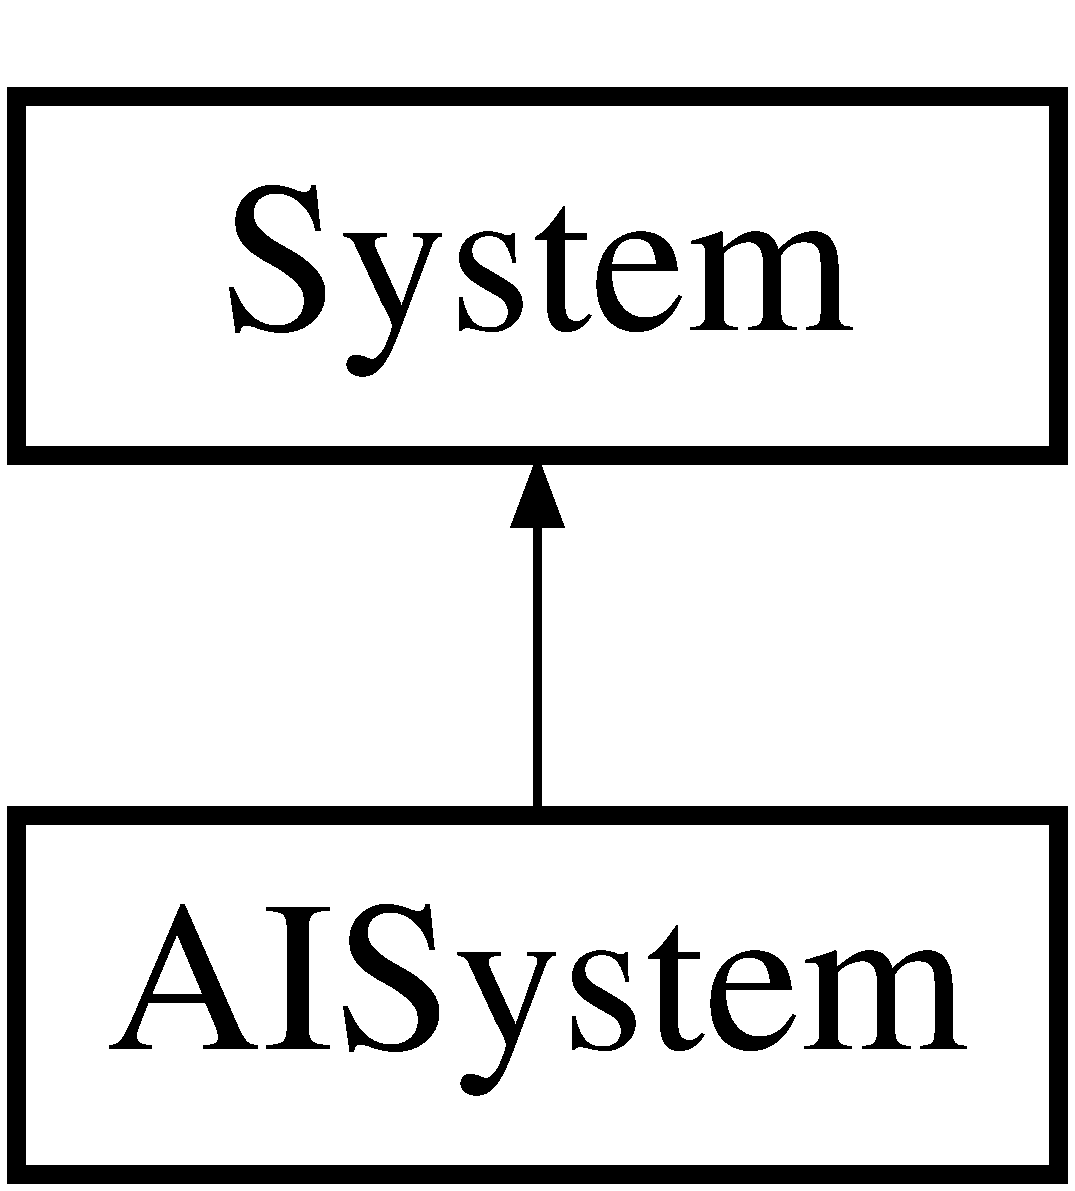
\includegraphics[height=2.000000cm]{class_a_i_system}
\end{center}
\end{figure}
\subsection*{Public Member Functions}
\begin{DoxyCompactItemize}
\item 
\hyperlink{class_a_i_system_a2b65c67d43bc5b2799ce2f4063e14cbc}{A\+I\+System} (\hyperlink{class_entity_system}{Entity\+System} \&)
\begin{DoxyCompactList}\small\item\em Constructor. \end{DoxyCompactList}\item 
\hyperlink{class_a_i_system_ad59d6780685228efb8fc5af54068897a}{$\sim$\+A\+I\+System} ()=default
\begin{DoxyCompactList}\small\item\em Destructor. \end{DoxyCompactList}\item 
void \hyperlink{class_a_i_system_a2c979ff5f110c79326f17f95c4b655d9}{update} (tdt\+::real) override
\begin{DoxyCompactList}\small\item\em Updates all valid entities by calling their update function stored in the A\+I\+Component\+::blueprint table. \end{DoxyCompactList}\item 
void \hyperlink{class_a_i_system_af5d48f605dc5ae79bed5976189e34510}{set\+\_\+update\+\_\+period} (tdt\+::real)
\begin{DoxyCompactList}\small\item\em Sets the amount of seconds it takes before the next AI update will be performed. \end{DoxyCompactList}\item 
tdt\+::real \hyperlink{class_a_i_system_a93a51bce77035a303024b5bfbefb040a}{get\+\_\+update\+\_\+period} () const 
\begin{DoxyCompactList}\small\item\em Returns the amount of seconds it takes before the next AI update will be performed. \end{DoxyCompactList}\item 
void \hyperlink{class_a_i_system_a6d1f35cb2ceddfcfa6cfc24531915160}{force\+\_\+update} ()
\begin{DoxyCompactList}\small\item\em Sets the update timer equal to the period and thus forcing all entities\textquotesingle{} AI to be updated on next \hyperlink{class_a_i_system_a2c979ff5f110c79326f17f95c4b655d9}{A\+I\+System\+::update} call. \end{DoxyCompactList}\end{DoxyCompactItemize}
\subsection*{Private Attributes}
\begin{DoxyCompactItemize}
\item 
\hyperlink{class_entity_system}{Entity\+System} \& \hyperlink{class_a_i_system_a5bb0fb45e68f716bee3d7c634a54fc55}{entities\+\_\+}
\begin{DoxyCompactList}\small\item\em Reference to the game\textquotesingle{}s entity system. \end{DoxyCompactList}\item 
tdt\+::real \hyperlink{class_a_i_system_a9e9d8e37dffa7b02b0e8b322c0f03c9b}{update\+\_\+timer\+\_\+}
\begin{DoxyCompactList}\small\item\em Used to track the time and check if the entities should be updated. \end{DoxyCompactList}\item 
tdt\+::real {\bfseries update\+\_\+period\+\_\+}\hypertarget{class_a_i_system_a59807402eb688a71028359302cb6755f}{}\label{class_a_i_system_a59807402eb688a71028359302cb6755f}

\end{DoxyCompactItemize}


\subsection{Detailed Description}
\hyperlink{class_system}{System} handling the AI of entities by calling their update method every frame. 

Definition at line 10 of file A\+I\+System.\+hpp.



\subsection{Constructor \& Destructor Documentation}
\index{A\+I\+System@{A\+I\+System}!A\+I\+System@{A\+I\+System}}
\index{A\+I\+System@{A\+I\+System}!A\+I\+System@{A\+I\+System}}
\subsubsection[{\texorpdfstring{A\+I\+System(\+Entity\+System \&)}{AISystem(EntitySystem &)}}]{\setlength{\rightskip}{0pt plus 5cm}A\+I\+System\+::\+A\+I\+System (
\begin{DoxyParamCaption}
\item[{{\bf Entity\+System} \&}]{ent}
\end{DoxyParamCaption}
)}\hypertarget{class_a_i_system_a2b65c67d43bc5b2799ce2f4063e14cbc}{}\label{class_a_i_system_a2b65c67d43bc5b2799ce2f4063e14cbc}


Constructor. 


\begin{DoxyParams}{Parameters}
{\em Reference} & to the game\textquotesingle{}s entity system. \\
\hline
\end{DoxyParams}


Definition at line 6 of file A\+I\+System.\+cpp.

\index{A\+I\+System@{A\+I\+System}!````~A\+I\+System@{$\sim$\+A\+I\+System}}
\index{````~A\+I\+System@{$\sim$\+A\+I\+System}!A\+I\+System@{A\+I\+System}}
\subsubsection[{\texorpdfstring{$\sim$\+A\+I\+System()=default}{~AISystem()=default}}]{\setlength{\rightskip}{0pt plus 5cm}A\+I\+System\+::$\sim$\+A\+I\+System (
\begin{DoxyParamCaption}
{}
\end{DoxyParamCaption}
)\hspace{0.3cm}{\ttfamily [default]}}\hypertarget{class_a_i_system_ad59d6780685228efb8fc5af54068897a}{}\label{class_a_i_system_ad59d6780685228efb8fc5af54068897a}


Destructor. 



\subsection{Member Function Documentation}
\index{A\+I\+System@{A\+I\+System}!force\+\_\+update@{force\+\_\+update}}
\index{force\+\_\+update@{force\+\_\+update}!A\+I\+System@{A\+I\+System}}
\subsubsection[{\texorpdfstring{force\+\_\+update()}{force_update()}}]{\setlength{\rightskip}{0pt plus 5cm}void A\+I\+System\+::force\+\_\+update (
\begin{DoxyParamCaption}
{}
\end{DoxyParamCaption}
)}\hypertarget{class_a_i_system_a6d1f35cb2ceddfcfa6cfc24531915160}{}\label{class_a_i_system_a6d1f35cb2ceddfcfa6cfc24531915160}


Sets the update timer equal to the period and thus forcing all entities\textquotesingle{} AI to be updated on next \hyperlink{class_a_i_system_a2c979ff5f110c79326f17f95c4b655d9}{A\+I\+System\+::update} call. 



Definition at line 42 of file A\+I\+System.\+cpp.

\index{A\+I\+System@{A\+I\+System}!get\+\_\+update\+\_\+period@{get\+\_\+update\+\_\+period}}
\index{get\+\_\+update\+\_\+period@{get\+\_\+update\+\_\+period}!A\+I\+System@{A\+I\+System}}
\subsubsection[{\texorpdfstring{get\+\_\+update\+\_\+period() const }{get_update_period() const }}]{\setlength{\rightskip}{0pt plus 5cm}tdt\+::real A\+I\+System\+::get\+\_\+update\+\_\+period (
\begin{DoxyParamCaption}
{}
\end{DoxyParamCaption}
) const}\hypertarget{class_a_i_system_a93a51bce77035a303024b5bfbefb040a}{}\label{class_a_i_system_a93a51bce77035a303024b5bfbefb040a}


Returns the amount of seconds it takes before the next AI update will be performed. 



Definition at line 37 of file A\+I\+System.\+cpp.

\index{A\+I\+System@{A\+I\+System}!set\+\_\+update\+\_\+period@{set\+\_\+update\+\_\+period}}
\index{set\+\_\+update\+\_\+period@{set\+\_\+update\+\_\+period}!A\+I\+System@{A\+I\+System}}
\subsubsection[{\texorpdfstring{set\+\_\+update\+\_\+period(tdt\+::real)}{set_update_period(tdt::real)}}]{\setlength{\rightskip}{0pt plus 5cm}void A\+I\+System\+::set\+\_\+update\+\_\+period (
\begin{DoxyParamCaption}
\item[{tdt\+::real}]{val}
\end{DoxyParamCaption}
)}\hypertarget{class_a_i_system_af5d48f605dc5ae79bed5976189e34510}{}\label{class_a_i_system_af5d48f605dc5ae79bed5976189e34510}


Sets the amount of seconds it takes before the next AI update will be performed. 


\begin{DoxyParams}{Parameters}
{\em Update} & period time (in seconds). \\
\hline
\end{DoxyParams}


Definition at line 32 of file A\+I\+System.\+cpp.

\index{A\+I\+System@{A\+I\+System}!update@{update}}
\index{update@{update}!A\+I\+System@{A\+I\+System}}
\subsubsection[{\texorpdfstring{update(tdt\+::real) override}{update(tdt::real) override}}]{\setlength{\rightskip}{0pt plus 5cm}void A\+I\+System\+::update (
\begin{DoxyParamCaption}
\item[{tdt\+::real}]{delta}
\end{DoxyParamCaption}
)\hspace{0.3cm}{\ttfamily [override]}, {\ttfamily [virtual]}}\hypertarget{class_a_i_system_a2c979ff5f110c79326f17f95c4b655d9}{}\label{class_a_i_system_a2c979ff5f110c79326f17f95c4b655d9}


Updates all valid entities by calling their update function stored in the A\+I\+Component\+::blueprint table. 


\begin{DoxyParams}{Parameters}
{\em Time} & since the last frame. \\
\hline
\end{DoxyParams}


Implements \hyperlink{class_system_a6d54c9bd38eb43d620a1451cb0925472}{System}.



Definition at line 10 of file A\+I\+System.\+cpp.



\subsection{Member Data Documentation}
\index{A\+I\+System@{A\+I\+System}!entities\+\_\+@{entities\+\_\+}}
\index{entities\+\_\+@{entities\+\_\+}!A\+I\+System@{A\+I\+System}}
\subsubsection[{\texorpdfstring{entities\+\_\+}{entities_}}]{\setlength{\rightskip}{0pt plus 5cm}{\bf Entity\+System}\& A\+I\+System\+::entities\+\_\+\hspace{0.3cm}{\ttfamily [private]}}\hypertarget{class_a_i_system_a5bb0fb45e68f716bee3d7c634a54fc55}{}\label{class_a_i_system_a5bb0fb45e68f716bee3d7c634a54fc55}


Reference to the game\textquotesingle{}s entity system. 



Definition at line 54 of file A\+I\+System.\+hpp.

\index{A\+I\+System@{A\+I\+System}!update\+\_\+timer\+\_\+@{update\+\_\+timer\+\_\+}}
\index{update\+\_\+timer\+\_\+@{update\+\_\+timer\+\_\+}!A\+I\+System@{A\+I\+System}}
\subsubsection[{\texorpdfstring{update\+\_\+timer\+\_\+}{update_timer_}}]{\setlength{\rightskip}{0pt plus 5cm}tdt\+::real A\+I\+System\+::update\+\_\+timer\+\_\+\hspace{0.3cm}{\ttfamily [private]}}\hypertarget{class_a_i_system_a9e9d8e37dffa7b02b0e8b322c0f03c9b}{}\label{class_a_i_system_a9e9d8e37dffa7b02b0e8b322c0f03c9b}


Used to track the time and check if the entities should be updated. 



Definition at line 59 of file A\+I\+System.\+hpp.



The documentation for this class was generated from the following files\+:\begin{DoxyCompactItemize}
\item 
systems/A\+I\+System.\+hpp\item 
systems/A\+I\+System.\+cpp\end{DoxyCompactItemize}

\hypertarget{struct_align_component}{}\section{Align\+Component Struct Reference}
\label{struct_align_component}\index{Align\+Component@{Align\+Component}}


Holds information about an objects align states, i.\+e.  




{\ttfamily \#include $<$Components.\+hpp$>$}

\subsection*{Classes}
\begin{DoxyCompactItemize}
\item 
struct \hyperlink{struct_align_component_1_1_align_state}{Align\+State}
\end{DoxyCompactItemize}
\subsection*{Public Member Functions}
\begin{DoxyCompactItemize}
\item 
{\bfseries Align\+Component} (const \hyperlink{struct_align_component}{Align\+Component} \&)=default\hypertarget{struct_align_component_a1eb416a6223ac7f9c1aee28e41100799}{}\label{struct_align_component_a1eb416a6223ac7f9c1aee28e41100799}

\item 
{\bfseries Align\+Component} (\hyperlink{struct_align_component}{Align\+Component} \&\&)=default\hypertarget{struct_align_component_a194311cf2534af85c0f064aed422c1af}{}\label{struct_align_component_a194311cf2534af85c0f064aed422c1af}

\item 
\hyperlink{struct_align_component}{Align\+Component} \& {\bfseries operator=} (const \hyperlink{struct_align_component}{Align\+Component} \&)=default\hypertarget{struct_align_component_a121621742f5c421c46f6669a8ccb9684}{}\label{struct_align_component_a121621742f5c421c46f6669a8ccb9684}

\item 
\hyperlink{struct_align_component}{Align\+Component} \& {\bfseries operator=} (\hyperlink{struct_align_component}{Align\+Component} \&\&)=default\hypertarget{struct_align_component_a097699c3fbfa6b02e2fa32ef08806b81}{}\label{struct_align_component_a097699c3fbfa6b02e2fa32ef08806b81}

\end{DoxyCompactItemize}
\subsection*{Public Attributes}
\begin{DoxyCompactItemize}
\item 
std\+::array$<$ \hyperlink{struct_align_component_1_1_align_state}{Align\+State}, state\+\_\+count $>$ {\bfseries states}\hypertarget{struct_align_component_a173543907cd141718dfb844b613abcb4}{}\label{struct_align_component_a173543907cd141718dfb844b613abcb4}

\end{DoxyCompactItemize}
\subsection*{Static Public Attributes}
\begin{DoxyCompactItemize}
\item 
static constexpr int {\bfseries type} = 24\hypertarget{struct_align_component_a0f9de2f94f3dd0212d74e71a56cbb411}{}\label{struct_align_component_a0f9de2f94f3dd0212d74e71a56cbb411}

\item 
static constexpr int {\bfseries state\+\_\+count} = 5\hypertarget{struct_align_component_ab553baa3b9884a4c9338cd66e1ab9e24}{}\label{struct_align_component_ab553baa3b9884a4c9338cd66e1ab9e24}

\end{DoxyCompactItemize}


\subsection{Detailed Description}
Holds information about an objects align states, i.\+e. 

scale, model, etc for the different alignments of blocks (e.\+g. walls). 

Definition at line 588 of file Components.\+hpp.



The documentation for this struct was generated from the following file\+:\begin{DoxyCompactItemize}
\item 
Components.\+hpp\end{DoxyCompactItemize}

\hypertarget{struct_align_component_1_1_align_state}{}\section{Align\+Component\+:\+:Align\+State Struct Reference}
\label{struct_align_component_1_1_align_state}\index{Align\+Component\+::\+Align\+State@{Align\+Component\+::\+Align\+State}}
\subsection*{Public Attributes}
\begin{DoxyCompactItemize}
\item 
Ogre\+::\+Vector3 {\bfseries scale}\hypertarget{struct_align_component_1_1_align_state_a23e6468e241f1efddf5e17883b8aa1ac}{}\label{struct_align_component_1_1_align_state_a23e6468e241f1efddf5e17883b8aa1ac}

\item 
Ogre\+::\+Vector3 {\bfseries position\+\_\+offset}\hypertarget{struct_align_component_1_1_align_state_a0b5fd1bff84997efe2f1a040d4c6506f}{}\label{struct_align_component_1_1_align_state_a0b5fd1bff84997efe2f1a040d4c6506f}

\item 
std\+::string {\bfseries mesh}\hypertarget{struct_align_component_1_1_align_state_aa3e812948ab2451b553844c6612325e7}{}\label{struct_align_component_1_1_align_state_aa3e812948ab2451b553844c6612325e7}

\item 
std\+::string {\bfseries material}\hypertarget{struct_align_component_1_1_align_state_ac80276905be3f5a6c6fc1f4afbb34420}{}\label{struct_align_component_1_1_align_state_ac80276905be3f5a6c6fc1f4afbb34420}

\end{DoxyCompactItemize}


\subsection{Detailed Description}


Definition at line 593 of file Components.\+hpp.



The documentation for this struct was generated from the following file\+:\begin{DoxyCompactItemize}
\item 
Components.\+hpp\end{DoxyCompactItemize}

\hypertarget{structutil_1_1path__type_1_1_b_e_s_t___p_a_t_h}{}\section{util\+:\+:path\+\_\+type\+:\+:B\+E\+S\+T\+\_\+\+P\+A\+TH Struct Reference}
\label{structutil_1_1path__type_1_1_b_e_s_t___p_a_t_h}\index{util\+::path\+\_\+type\+::\+B\+E\+S\+T\+\_\+\+P\+A\+TH@{util\+::path\+\_\+type\+::\+B\+E\+S\+T\+\_\+\+P\+A\+TH}}


Finds the best path by refusing any paths found.  




{\ttfamily \#include $<$Pathfinding\+Algorithms.\+hpp$>$}

\subsection*{Static Public Member Functions}
\begin{DoxyCompactItemize}
\item 
static bool {\bfseries return\+\_\+path} ()\hypertarget{structutil_1_1path__type_1_1_b_e_s_t___p_a_t_h_a61f3304ea997981f8e29774c3b2a56c8}{}\label{structutil_1_1path__type_1_1_b_e_s_t___p_a_t_h_a61f3304ea997981f8e29774c3b2a56c8}

\end{DoxyCompactItemize}


\subsection{Detailed Description}
Finds the best path by refusing any paths found. 

Definition at line 143 of file Pathfinding\+Algorithms.\+hpp.



The documentation for this struct was generated from the following file\+:\begin{DoxyCompactItemize}
\item 
tools/Pathfinding\+Algorithms.\+hpp\end{DoxyCompactItemize}

\hypertarget{class_builder_window}{}\section{Builder\+Window Class Reference}
\label{class_builder_window}\index{Builder\+Window@{Builder\+Window}}


Class representing the building selection window, allows the player to place registered (unlocked) buildings.  




{\ttfamily \#include $<$Builder\+Window.\+hpp$>$}

Inheritance diagram for Builder\+Window\+:\begin{figure}[H]
\begin{center}
\leavevmode
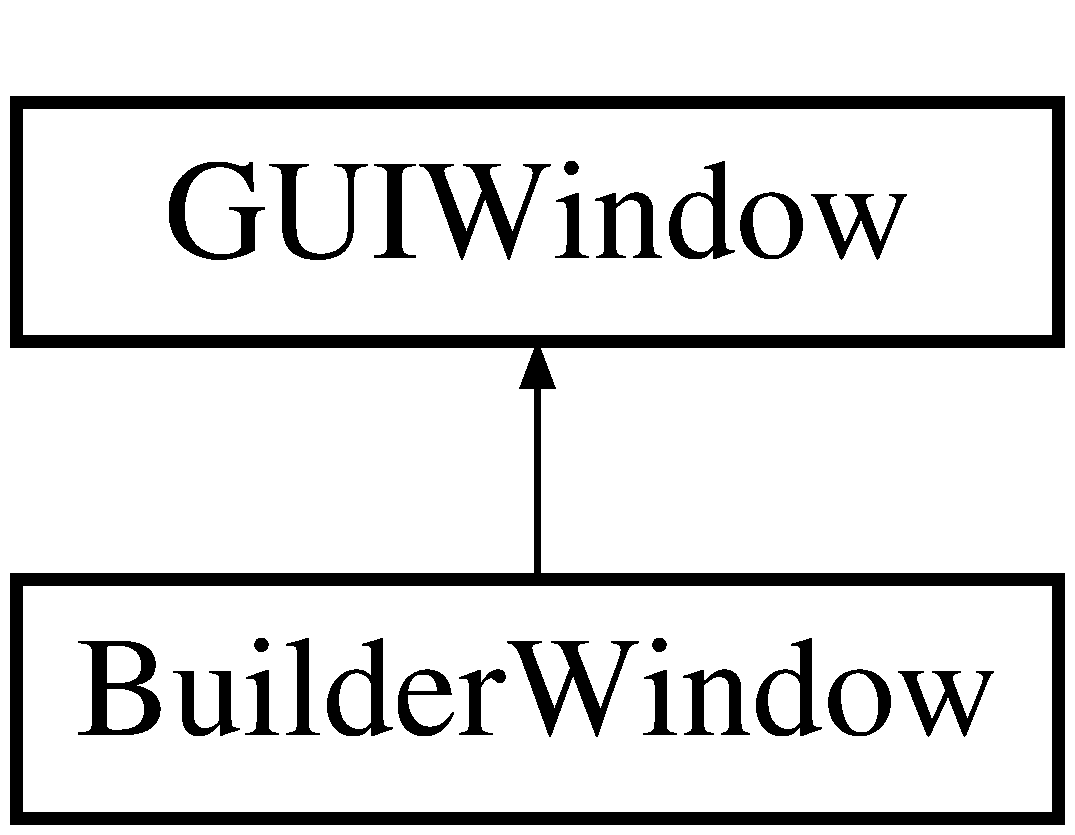
\includegraphics[height=2.000000cm]{class_builder_window}
\end{center}
\end{figure}
\subsection*{Public Member Functions}
\begin{DoxyCompactItemize}
\item 
\hyperlink{class_builder_window_af03a3f27f3a1025f1d992e62b6549631}{Builder\+Window} ()
\begin{DoxyCompactList}\small\item\em Constructor. \end{DoxyCompactList}\item 
\hyperlink{class_builder_window_a974a89e16f9c2ede36b2a8dddaac334e}{$\sim$\+Builder\+Window} ()=default
\begin{DoxyCompactList}\small\item\em Destructor. \end{DoxyCompactList}\item 
void \hyperlink{class_builder_window_a0c6d38cbbcf6725e0ac6257306cceba7}{register\+\_\+building} (const std\+::string \&)
\begin{DoxyCompactList}\small\item\em Appends a table name to the vector of all building tables. \end{DoxyCompactList}\item 
void \hyperlink{class_builder_window_a3b3c1fe120624d0109cd8714ad7b3e09}{set\+\_\+placer} (\hyperlink{class_entity_placer}{Entity\+Placer} $\ast$)
\begin{DoxyCompactList}\small\item\em Sets the placer that is used to build. \end{DoxyCompactList}\item 
const std\+::vector$<$ std\+::string $>$ \& \hyperlink{class_builder_window_a6427ac456e5ce78ca3058c2355bab90f}{get\+\_\+buildings} () const 
\begin{DoxyCompactList}\small\item\em Returns a vector containing all the names of the registered buildings. \end{DoxyCompactList}\item 
void \hyperlink{class_builder_window_aa21ded0717c9698b7a71a00d5f3460c0}{clear\+\_\+buildings} ()
\begin{DoxyCompactList}\small\item\em Removes all unlocked buildings. \end{DoxyCompactList}\item 
void \hyperlink{class_builder_window_a8fb26ae5886f86ab21a1a3e1dc9b2b98}{build} (int)
\begin{DoxyCompactList}\small\item\em Places the building on a given position. \end{DoxyCompactList}\item 
void \hyperlink{class_builder_window_a648d7e9097ccaf913c047ab5a6654049}{dec\+\_\+selection} ()
\begin{DoxyCompactList}\small\item\em Decrements selection\+\_\+number\+\_\+ by one and updates the window. \end{DoxyCompactList}\item 
void \hyperlink{class_builder_window_ae74b14919ee458c9a241454233437428}{inc\+\_\+selection} ()
\begin{DoxyCompactList}\small\item\em Increments selection\+\_\+number\+\_\+ by one and updates the window. \end{DoxyCompactList}\end{DoxyCompactItemize}
\subsection*{Protected Member Functions}
\begin{DoxyCompactItemize}
\item 
void \hyperlink{class_builder_window_aadd9fb46ddd55ce86bff0f012f56f2e8}{init\+\_\+} () override
\begin{DoxyCompactList}\small\item\em Initializes the window and subscribes events. \end{DoxyCompactList}\end{DoxyCompactItemize}
\subsection*{Private Member Functions}
\begin{DoxyCompactItemize}
\item 
const std\+::string \& \hyperlink{class_builder_window_a1218facb3b07955dc9335e33cbf34031}{get\+\_\+building\+\_\+} (std\+::size\+\_\+t)
\begin{DoxyCompactList}\small\item\em Range checked buildings\+\_\+ index access, returns the name of the building at a given index or \char`\"{}\+U\+N\+K\+N\+O\+W\+N\char`\"{} if the index is out of bounds. \end{DoxyCompactList}\item 
void \hyperlink{class_builder_window_af0bd0684025576217acb9ddca8ee7377}{update\+\_\+selection\+\_\+} ()
\begin{DoxyCompactList}\small\item\em Updates building names on the buttons. \end{DoxyCompactList}\end{DoxyCompactItemize}
\subsection*{Private Attributes}
\begin{DoxyCompactItemize}
\item 
std\+::vector$<$ std\+::string $>$ \hyperlink{class_builder_window_a9ca2c3d5feabdea04f1f17251dd7049b}{buildings\+\_\+}
\begin{DoxyCompactList}\small\item\em Names of all registered buildings. \end{DoxyCompactList}\item 
std\+::size\+\_\+t \hyperlink{class_builder_window_a5b5d32587a7434ba28856d98ea5b99de}{selection\+\_\+number\+\_\+}
\begin{DoxyCompactList}\small\item\em Number of the current rightmost selection. \end{DoxyCompactList}\item 
\hyperlink{class_entity_placer}{Entity\+Placer} $\ast$ \hyperlink{class_builder_window_ac2eee6525635c8b108b48a3a7d382d82}{placer\+\_\+}
\begin{DoxyCompactList}\small\item\em Placer used to build. \end{DoxyCompactList}\end{DoxyCompactItemize}
\subsection*{Additional Inherited Members}


\subsection{Detailed Description}
Class representing the building selection window, allows the player to place registered (unlocked) buildings. 

Definition at line 12 of file Builder\+Window.\+hpp.



\subsection{Constructor \& Destructor Documentation}
\index{Builder\+Window@{Builder\+Window}!Builder\+Window@{Builder\+Window}}
\index{Builder\+Window@{Builder\+Window}!Builder\+Window@{Builder\+Window}}
\subsubsection[{\texorpdfstring{Builder\+Window()}{BuilderWindow()}}]{\setlength{\rightskip}{0pt plus 5cm}Builder\+Window\+::\+Builder\+Window (
\begin{DoxyParamCaption}
{}
\end{DoxyParamCaption}
)}\hypertarget{class_builder_window_af03a3f27f3a1025f1d992e62b6549631}{}\label{class_builder_window_af03a3f27f3a1025f1d992e62b6549631}


Constructor. 



Definition at line 5 of file Builder\+Window.\+cpp.

\index{Builder\+Window@{Builder\+Window}!````~Builder\+Window@{$\sim$\+Builder\+Window}}
\index{````~Builder\+Window@{$\sim$\+Builder\+Window}!Builder\+Window@{Builder\+Window}}
\subsubsection[{\texorpdfstring{$\sim$\+Builder\+Window()=default}{~BuilderWindow()=default}}]{\setlength{\rightskip}{0pt plus 5cm}Builder\+Window\+::$\sim$\+Builder\+Window (
\begin{DoxyParamCaption}
{}
\end{DoxyParamCaption}
)\hspace{0.3cm}{\ttfamily [default]}}\hypertarget{class_builder_window_a974a89e16f9c2ede36b2a8dddaac334e}{}\label{class_builder_window_a974a89e16f9c2ede36b2a8dddaac334e}


Destructor. 



\subsection{Member Function Documentation}
\index{Builder\+Window@{Builder\+Window}!build@{build}}
\index{build@{build}!Builder\+Window@{Builder\+Window}}
\subsubsection[{\texorpdfstring{build(int)}{build(int)}}]{\setlength{\rightskip}{0pt plus 5cm}void Builder\+Window\+::build (
\begin{DoxyParamCaption}
\item[{int}]{build\+\_\+num}
\end{DoxyParamCaption}
)}\hypertarget{class_builder_window_a8fb26ae5886f86ab21a1a3e1dc9b2b98}{}\label{class_builder_window_a8fb26ae5886f86ab21a1a3e1dc9b2b98}


Places the building on a given position. 


\begin{DoxyParams}{Parameters}
{\em The} & button position. (1-\/4) \\
\hline
\end{DoxyParams}


Definition at line 37 of file Builder\+Window.\+cpp.

\index{Builder\+Window@{Builder\+Window}!clear\+\_\+buildings@{clear\+\_\+buildings}}
\index{clear\+\_\+buildings@{clear\+\_\+buildings}!Builder\+Window@{Builder\+Window}}
\subsubsection[{\texorpdfstring{clear\+\_\+buildings()}{clear_buildings()}}]{\setlength{\rightskip}{0pt plus 5cm}void Builder\+Window\+::clear\+\_\+buildings (
\begin{DoxyParamCaption}
{}
\end{DoxyParamCaption}
)}\hypertarget{class_builder_window_aa21ded0717c9698b7a71a00d5f3460c0}{}\label{class_builder_window_aa21ded0717c9698b7a71a00d5f3460c0}


Removes all unlocked buildings. 



Definition at line 30 of file Builder\+Window.\+cpp.

\index{Builder\+Window@{Builder\+Window}!dec\+\_\+selection@{dec\+\_\+selection}}
\index{dec\+\_\+selection@{dec\+\_\+selection}!Builder\+Window@{Builder\+Window}}
\subsubsection[{\texorpdfstring{dec\+\_\+selection()}{dec_selection()}}]{\setlength{\rightskip}{0pt plus 5cm}void Builder\+Window\+::dec\+\_\+selection (
\begin{DoxyParamCaption}
{}
\end{DoxyParamCaption}
)}\hypertarget{class_builder_window_a648d7e9097ccaf913c047ab5a6654049}{}\label{class_builder_window_a648d7e9097ccaf913c047ab5a6654049}


Decrements selection\+\_\+number\+\_\+ by one and updates the window. 



Definition at line 101 of file Builder\+Window.\+cpp.

\index{Builder\+Window@{Builder\+Window}!get\+\_\+building\+\_\+@{get\+\_\+building\+\_\+}}
\index{get\+\_\+building\+\_\+@{get\+\_\+building\+\_\+}!Builder\+Window@{Builder\+Window}}
\subsubsection[{\texorpdfstring{get\+\_\+building\+\_\+(std\+::size\+\_\+t)}{get_building_(std::size_t)}}]{\setlength{\rightskip}{0pt plus 5cm}const std\+::string \& Builder\+Window\+::get\+\_\+building\+\_\+ (
\begin{DoxyParamCaption}
\item[{std\+::size\+\_\+t}]{index}
\end{DoxyParamCaption}
)\hspace{0.3cm}{\ttfamily [private]}}\hypertarget{class_builder_window_a1218facb3b07955dc9335e33cbf34031}{}\label{class_builder_window_a1218facb3b07955dc9335e33cbf34031}


Range checked buildings\+\_\+ index access, returns the name of the building at a given index or \char`\"{}\+U\+N\+K\+N\+O\+W\+N\char`\"{} if the index is out of bounds. 


\begin{DoxyParams}{Parameters}
{\em Index} & of the building in the buildings\+\_\+ vector. \\
\hline
\end{DoxyParams}


Definition at line 119 of file Builder\+Window.\+cpp.

\index{Builder\+Window@{Builder\+Window}!get\+\_\+buildings@{get\+\_\+buildings}}
\index{get\+\_\+buildings@{get\+\_\+buildings}!Builder\+Window@{Builder\+Window}}
\subsubsection[{\texorpdfstring{get\+\_\+buildings() const }{get_buildings() const }}]{\setlength{\rightskip}{0pt plus 5cm}const std\+::vector$<$ std\+::string $>$ \& Builder\+Window\+::get\+\_\+buildings (
\begin{DoxyParamCaption}
{}
\end{DoxyParamCaption}
) const}\hypertarget{class_builder_window_a6427ac456e5ce78ca3058c2355bab90f}{}\label{class_builder_window_a6427ac456e5ce78ca3058c2355bab90f}


Returns a vector containing all the names of the registered buildings. 

(Used for serialization.) 

Definition at line 25 of file Builder\+Window.\+cpp.

\index{Builder\+Window@{Builder\+Window}!inc\+\_\+selection@{inc\+\_\+selection}}
\index{inc\+\_\+selection@{inc\+\_\+selection}!Builder\+Window@{Builder\+Window}}
\subsubsection[{\texorpdfstring{inc\+\_\+selection()}{inc_selection()}}]{\setlength{\rightskip}{0pt plus 5cm}void Builder\+Window\+::inc\+\_\+selection (
\begin{DoxyParamCaption}
{}
\end{DoxyParamCaption}
)}\hypertarget{class_builder_window_ae74b14919ee458c9a241454233437428}{}\label{class_builder_window_ae74b14919ee458c9a241454233437428}


Increments selection\+\_\+number\+\_\+ by one and updates the window. 



Definition at line 110 of file Builder\+Window.\+cpp.

\index{Builder\+Window@{Builder\+Window}!init\+\_\+@{init\+\_\+}}
\index{init\+\_\+@{init\+\_\+}!Builder\+Window@{Builder\+Window}}
\subsubsection[{\texorpdfstring{init\+\_\+() override}{init_() override}}]{\setlength{\rightskip}{0pt plus 5cm}void Builder\+Window\+::init\+\_\+ (
\begin{DoxyParamCaption}
{}
\end{DoxyParamCaption}
)\hspace{0.3cm}{\ttfamily [override]}, {\ttfamily [protected]}, {\ttfamily [virtual]}}\hypertarget{class_builder_window_aadd9fb46ddd55ce86bff0f012f56f2e8}{}\label{class_builder_window_aadd9fb46ddd55ce86bff0f012f56f2e8}


Initializes the window and subscribes events. 



Implements \hyperlink{class_g_u_i_window_a2a7c011363f401a57a26cc7c7652bdfd}{G\+U\+I\+Window}.



Definition at line 48 of file Builder\+Window.\+cpp.

\index{Builder\+Window@{Builder\+Window}!register\+\_\+building@{register\+\_\+building}}
\index{register\+\_\+building@{register\+\_\+building}!Builder\+Window@{Builder\+Window}}
\subsubsection[{\texorpdfstring{register\+\_\+building(const std\+::string \&)}{register_building(const std::string &)}}]{\setlength{\rightskip}{0pt plus 5cm}void Builder\+Window\+::register\+\_\+building (
\begin{DoxyParamCaption}
\item[{const std\+::string \&}]{tname}
\end{DoxyParamCaption}
)}\hypertarget{class_builder_window_a0c6d38cbbcf6725e0ac6257306cceba7}{}\label{class_builder_window_a0c6d38cbbcf6725e0ac6257306cceba7}


Appends a table name to the vector of all building tables. 


\begin{DoxyParams}{Parameters}
{\em Name} & of the table to register. \\
\hline
\end{DoxyParams}


Definition at line 9 of file Builder\+Window.\+cpp.

\index{Builder\+Window@{Builder\+Window}!set\+\_\+placer@{set\+\_\+placer}}
\index{set\+\_\+placer@{set\+\_\+placer}!Builder\+Window@{Builder\+Window}}
\subsubsection[{\texorpdfstring{set\+\_\+placer(\+Entity\+Placer $\ast$)}{set_placer(EntityPlacer *)}}]{\setlength{\rightskip}{0pt plus 5cm}void Builder\+Window\+::set\+\_\+placer (
\begin{DoxyParamCaption}
\item[{{\bf Entity\+Placer} $\ast$}]{p}
\end{DoxyParamCaption}
)}\hypertarget{class_builder_window_a3b3c1fe120624d0109cd8714ad7b3e09}{}\label{class_builder_window_a3b3c1fe120624d0109cd8714ad7b3e09}


Sets the placer that is used to build. 


\begin{DoxyParams}{Parameters}
{\em The} & new entity placer. \\
\hline
\end{DoxyParams}


Definition at line 20 of file Builder\+Window.\+cpp.

\index{Builder\+Window@{Builder\+Window}!update\+\_\+selection\+\_\+@{update\+\_\+selection\+\_\+}}
\index{update\+\_\+selection\+\_\+@{update\+\_\+selection\+\_\+}!Builder\+Window@{Builder\+Window}}
\subsubsection[{\texorpdfstring{update\+\_\+selection\+\_\+()}{update_selection_()}}]{\setlength{\rightskip}{0pt plus 5cm}void Builder\+Window\+::update\+\_\+selection\+\_\+ (
\begin{DoxyParamCaption}
{}
\end{DoxyParamCaption}
)\hspace{0.3cm}{\ttfamily [private]}}\hypertarget{class_builder_window_af0bd0684025576217acb9ddca8ee7377}{}\label{class_builder_window_af0bd0684025576217acb9ddca8ee7377}


Updates building names on the buttons. 



Definition at line 129 of file Builder\+Window.\+cpp.



\subsection{Member Data Documentation}
\index{Builder\+Window@{Builder\+Window}!buildings\+\_\+@{buildings\+\_\+}}
\index{buildings\+\_\+@{buildings\+\_\+}!Builder\+Window@{Builder\+Window}}
\subsubsection[{\texorpdfstring{buildings\+\_\+}{buildings_}}]{\setlength{\rightskip}{0pt plus 5cm}std\+::vector$<$std\+::string$>$ Builder\+Window\+::buildings\+\_\+\hspace{0.3cm}{\ttfamily [private]}}\hypertarget{class_builder_window_a9ca2c3d5feabdea04f1f17251dd7049b}{}\label{class_builder_window_a9ca2c3d5feabdea04f1f17251dd7049b}


Names of all registered buildings. 



Definition at line 89 of file Builder\+Window.\+hpp.

\index{Builder\+Window@{Builder\+Window}!placer\+\_\+@{placer\+\_\+}}
\index{placer\+\_\+@{placer\+\_\+}!Builder\+Window@{Builder\+Window}}
\subsubsection[{\texorpdfstring{placer\+\_\+}{placer_}}]{\setlength{\rightskip}{0pt plus 5cm}{\bf Entity\+Placer}$\ast$ Builder\+Window\+::placer\+\_\+\hspace{0.3cm}{\ttfamily [private]}}\hypertarget{class_builder_window_ac2eee6525635c8b108b48a3a7d382d82}{}\label{class_builder_window_ac2eee6525635c8b108b48a3a7d382d82}


Placer used to build. 



Definition at line 100 of file Builder\+Window.\+hpp.

\index{Builder\+Window@{Builder\+Window}!selection\+\_\+number\+\_\+@{selection\+\_\+number\+\_\+}}
\index{selection\+\_\+number\+\_\+@{selection\+\_\+number\+\_\+}!Builder\+Window@{Builder\+Window}}
\subsubsection[{\texorpdfstring{selection\+\_\+number\+\_\+}{selection_number_}}]{\setlength{\rightskip}{0pt plus 5cm}std\+::size\+\_\+t Builder\+Window\+::selection\+\_\+number\+\_\+\hspace{0.3cm}{\ttfamily [private]}}\hypertarget{class_builder_window_a5b5d32587a7434ba28856d98ea5b99de}{}\label{class_builder_window_a5b5d32587a7434ba28856d98ea5b99de}


Number of the current rightmost selection. 

The window shows buildings with indices $<$selection\+\_\+number\+\_\+ -\/ 3, selection\+\_\+number\+\_\+$>$. 

Definition at line 95 of file Builder\+Window.\+hpp.



The documentation for this class was generated from the following files\+:\begin{DoxyCompactItemize}
\item 
gui/Builder\+Window.\+hpp\item 
gui/Builder\+Window.\+cpp\end{DoxyCompactItemize}

\hypertarget{class_camera}{}\section{Camera Class Reference}
\label{class_camera}\index{Camera@{Camera}}


Class wrapping the Ogre camera object, allowing R\+T\+S-\/like movement and switching to free mode.  




{\ttfamily \#include $<$Camera.\+hpp$>$}

\subsection*{Public Member Functions}
\begin{DoxyCompactItemize}
\item 
\hyperlink{class_camera_ae23af4d7cab430c77d537621cdd16b3f}{Camera} ()=default
\begin{DoxyCompactList}\small\item\em Constructor. \end{DoxyCompactList}\item 
\hyperlink{class_camera_adcb96efefa7af58e3ee6534b15d4979b}{$\sim$\+Camera} ()=default
\begin{DoxyCompactList}\small\item\em Destructor. \end{DoxyCompactList}\item 
void \hyperlink{class_camera_a8e44e7aa45c25d149c64df40f6b67d44}{init} (Ogre\+::\+Camera $\ast$)
\begin{DoxyCompactList}\small\item\em Initializes the wrapper with a camera object. \end{DoxyCompactList}\item 
void \hyperlink{class_camera_a7ec17fe707671c1cb7ca4c0625708774}{set\+\_\+position} (const Ogre\+::\+Vector2 \&)
\begin{DoxyCompactList}\small\item\em Sets the 2D position of the camera (X and Z axes). \end{DoxyCompactList}\item 
const Ogre\+::\+Vector3 \& \hyperlink{class_camera_a3738ea5dd3673a13f54cfb7d1e605ce9}{get\+\_\+position} () const 
\begin{DoxyCompactList}\small\item\em Returns the 3D position of the camera (including height). \end{DoxyCompactList}\item 
void \hyperlink{class_camera_a66f1813809223a6746fb8a1c61961f0b}{set\+\_\+direction} (const Ogre\+::\+Vector3 \&)
\begin{DoxyCompactList}\small\item\em Changes the direction the camera is facing. \end{DoxyCompactList}\item 
const Ogre\+::\+Vector3 \& \hyperlink{class_camera_a572e91046d5610127d670dce74fb0b5e}{get\+\_\+direction} () const 
\begin{DoxyCompactList}\small\item\em Returns the direction the camera is facing. \end{DoxyCompactList}\item 
void \hyperlink{class_camera_ab7006a32d1c68a2e09f5aa1f19bf1e8e}{look\+\_\+at} (const Ogre\+::\+Vector2 \&)
\begin{DoxyCompactList}\small\item\em Makes the camera to look at a point on the ground. \end{DoxyCompactList}\item 
void \hyperlink{class_camera_a02be8aa0dbef77e02dddc715a726fb67}{reset} ()
\begin{DoxyCompactList}\small\item\em Resets the camera\textquotesingle{}s position and orientation. \end{DoxyCompactList}\item 
void \hyperlink{class_camera_ad24346aabd2c3a334b6a4b8c0bb433b6}{set\+\_\+start} (const Ogre\+::\+Vector2 \&, const Ogre\+::\+Vector2 \&, tdt\+::real)
\begin{DoxyCompactList}\small\item\em Sets the starting stats of the camera. \end{DoxyCompactList}\item 
void \hyperlink{class_camera_a320542638be37fd4a49014f87d7beb41}{set\+\_\+free\+\_\+mode} (bool)
\begin{DoxyCompactList}\small\item\em Changes the movement mode of the camera. \end{DoxyCompactList}\item 
bool \hyperlink{class_camera_a8cecaca1545eae90bf7e291a0b9c4cf9}{get\+\_\+free\+\_\+mode} () const 
\begin{DoxyCompactList}\small\item\em Returns true if the camera is in free mode, false otherwise. \end{DoxyCompactList}\item 
void \hyperlink{class_camera_a643abf766752b1ac87ccadf012f97a0a}{update} (tdt\+::real)
\begin{DoxyCompactList}\small\item\em Updates the movement of the camera. \end{DoxyCompactList}\item 
void \hyperlink{class_camera_a90965d8c49dd607024c9746f3b58709d}{key\+\_\+pressed} (C\+E\+G\+U\+I\+::\+Key\+::\+Scan)
\begin{DoxyCompactList}\small\item\em Moves the camera if a movement key was pressed. \end{DoxyCompactList}\item 
void \hyperlink{class_camera_a1b10287c63e826afd3a92ba3d2cc183e}{key\+\_\+released} (C\+E\+G\+U\+I\+::\+Key\+::\+Scan)
\begin{DoxyCompactList}\small\item\em Moves the camera if a movement key was released. \end{DoxyCompactList}\item 
void \hyperlink{class_camera_a9c5d8b3c9536959b6cf7d64a272903bb}{move} (D\+I\+R\+E\+C\+T\+I\+O\+N\+::\+V\+AL, tdt\+::real)
\begin{DoxyCompactList}\small\item\em Moves the camera in a given direction, used for mouse movement. \end{DoxyCompactList}\item 
void \hyperlink{class_camera_a7e6994e657a5261708bf10915917fbcf}{set\+\_\+height} (tdt\+::real)
\begin{DoxyCompactList}\small\item\em Changes the height of the camera. \end{DoxyCompactList}\item 
tdt\+::real \hyperlink{class_camera_aa81c361011aedca6052a628029c4d422}{get\+\_\+height} () const 
\begin{DoxyCompactList}\small\item\em Returns the height of the camera. \end{DoxyCompactList}\item 
void \hyperlink{class_camera_aab2a0949e1dcdc92f1ba32f6edcb194c}{pitch} (const Ogre\+::\+Degree \&)
\begin{DoxyCompactList}\small\item\em Rotates the camera around the side-\/to-\/side axis. \end{DoxyCompactList}\item 
void \hyperlink{class_camera_ac48d23d230089a006ffd5e3ec154358b}{yaw} (const Ogre\+::\+Degree \&)
\begin{DoxyCompactList}\small\item\em Rotates the camera around the vertical axis. \end{DoxyCompactList}\end{DoxyCompactItemize}
\subsection*{Private Attributes}
\begin{DoxyCompactItemize}
\item 
Ogre\+::\+Camera $\ast$ \hyperlink{class_camera_a03027c3c0af67ea450e4df182d3ade68}{camera\+\_\+}
\begin{DoxyCompactList}\small\item\em Ogre camera that is wrapped. \end{DoxyCompactList}\item 
std\+::tuple$<$ Ogre\+::\+Vector3, Ogre\+::\+Vector3 $>$ \hyperlink{class_camera_a050ad880982ac8d843b1b66dd6431170}{start\+\_\+}
\begin{DoxyCompactList}\small\item\em Starting stats of the camera, used when resetting. \end{DoxyCompactList}\item 
bool \hyperlink{class_camera_ab9e64d468f4bdc04492a6a326c8dc2ff}{free\+\_\+mode\+\_\+}
\begin{DoxyCompactList}\small\item\em Determines the mode of the camera, if true, it can fly around the level, if false, it can move in an R\+T\+S-\/like fashion. \end{DoxyCompactList}\item 
Ogre\+::\+Vector3 \hyperlink{class_camera_aa3b2cb044a4fd23eb8b3426e10ad0393}{movement\+\_\+direction\+\_\+}
\begin{DoxyCompactList}\small\item\em Direction vector of the free mode movement. \end{DoxyCompactList}\item 
tdt\+::real \hyperlink{class_camera_a08f8fa9c6bf80dcafe14d54787300ade}{speed\+\_\+}
\begin{DoxyCompactList}\small\item\em Speed modifier of the camera. \end{DoxyCompactList}\item 
tdt\+::real \hyperlink{class_camera_ab1238ca5c0a615278712ff93c50c095b}{height\+\_\+}
\begin{DoxyCompactList}\small\item\em Y axis the camera is locked at when free mode is disabled. \end{DoxyCompactList}\end{DoxyCompactItemize}
\subsection*{Friends}
\begin{DoxyCompactItemize}
\item 
class {\bfseries Game\+Serializer}\hypertarget{class_camera_a6f4a2258d01e962995f3a4743b711864}{}\label{class_camera_a6f4a2258d01e962995f3a4743b711864}

\item 
class {\bfseries Game}\hypertarget{class_camera_aa2fab026580d6f14280c2ffb8063a314}{}\label{class_camera_aa2fab026580d6f14280c2ffb8063a314}

\end{DoxyCompactItemize}


\subsection{Detailed Description}
Class wrapping the Ogre camera object, allowing R\+T\+S-\/like movement and switching to free mode. 

Definition at line 13 of file Camera.\+hpp.



\subsection{Constructor \& Destructor Documentation}
\index{Camera@{Camera}!Camera@{Camera}}
\index{Camera@{Camera}!Camera@{Camera}}
\subsubsection[{\texorpdfstring{Camera()=default}{Camera()=default}}]{\setlength{\rightskip}{0pt plus 5cm}Camera\+::\+Camera (
\begin{DoxyParamCaption}
{}
\end{DoxyParamCaption}
)\hspace{0.3cm}{\ttfamily [default]}}\hypertarget{class_camera_ae23af4d7cab430c77d537621cdd16b3f}{}\label{class_camera_ae23af4d7cab430c77d537621cdd16b3f}


Constructor. 

\index{Camera@{Camera}!````~Camera@{$\sim$\+Camera}}
\index{````~Camera@{$\sim$\+Camera}!Camera@{Camera}}
\subsubsection[{\texorpdfstring{$\sim$\+Camera()=default}{~Camera()=default}}]{\setlength{\rightskip}{0pt plus 5cm}Camera\+::$\sim$\+Camera (
\begin{DoxyParamCaption}
{}
\end{DoxyParamCaption}
)\hspace{0.3cm}{\ttfamily [default]}}\hypertarget{class_camera_adcb96efefa7af58e3ee6534b15d4979b}{}\label{class_camera_adcb96efefa7af58e3ee6534b15d4979b}


Destructor. 



\subsection{Member Function Documentation}
\index{Camera@{Camera}!get\+\_\+direction@{get\+\_\+direction}}
\index{get\+\_\+direction@{get\+\_\+direction}!Camera@{Camera}}
\subsubsection[{\texorpdfstring{get\+\_\+direction() const }{get_direction() const }}]{\setlength{\rightskip}{0pt plus 5cm}const Ogre\+::\+Vector3 \& Camera\+::get\+\_\+direction (
\begin{DoxyParamCaption}
{}
\end{DoxyParamCaption}
) const}\hypertarget{class_camera_a572e91046d5610127d670dce74fb0b5e}{}\label{class_camera_a572e91046d5610127d670dce74fb0b5e}


Returns the direction the camera is facing. 



Definition at line 27 of file Camera.\+cpp.

\index{Camera@{Camera}!get\+\_\+free\+\_\+mode@{get\+\_\+free\+\_\+mode}}
\index{get\+\_\+free\+\_\+mode@{get\+\_\+free\+\_\+mode}!Camera@{Camera}}
\subsubsection[{\texorpdfstring{get\+\_\+free\+\_\+mode() const }{get_free_mode() const }}]{\setlength{\rightskip}{0pt plus 5cm}bool Camera\+::get\+\_\+free\+\_\+mode (
\begin{DoxyParamCaption}
{}
\end{DoxyParamCaption}
) const}\hypertarget{class_camera_a8cecaca1545eae90bf7e291a0b9c4cf9}{}\label{class_camera_a8cecaca1545eae90bf7e291a0b9c4cf9}


Returns true if the camera is in free mode, false otherwise. 



Definition at line 60 of file Camera.\+cpp.

\index{Camera@{Camera}!get\+\_\+height@{get\+\_\+height}}
\index{get\+\_\+height@{get\+\_\+height}!Camera@{Camera}}
\subsubsection[{\texorpdfstring{get\+\_\+height() const }{get_height() const }}]{\setlength{\rightskip}{0pt plus 5cm}tdt\+::real Camera\+::get\+\_\+height (
\begin{DoxyParamCaption}
{}
\end{DoxyParamCaption}
) const}\hypertarget{class_camera_aa81c361011aedca6052a628029c4d422}{}\label{class_camera_aa81c361011aedca6052a628029c4d422}


Returns the height of the camera. 



Definition at line 163 of file Camera.\+cpp.

\index{Camera@{Camera}!get\+\_\+position@{get\+\_\+position}}
\index{get\+\_\+position@{get\+\_\+position}!Camera@{Camera}}
\subsubsection[{\texorpdfstring{get\+\_\+position() const }{get_position() const }}]{\setlength{\rightskip}{0pt plus 5cm}const Ogre\+::\+Vector3 \& Camera\+::get\+\_\+position (
\begin{DoxyParamCaption}
{}
\end{DoxyParamCaption}
) const}\hypertarget{class_camera_a3738ea5dd3673a13f54cfb7d1e605ce9}{}\label{class_camera_a3738ea5dd3673a13f54cfb7d1e605ce9}


Returns the 3D position of the camera (including height). 



Definition at line 16 of file Camera.\+cpp.

\index{Camera@{Camera}!init@{init}}
\index{init@{init}!Camera@{Camera}}
\subsubsection[{\texorpdfstring{init(\+Ogre\+::\+Camera $\ast$)}{init(Ogre::Camera *)}}]{\setlength{\rightskip}{0pt plus 5cm}void Camera\+::init (
\begin{DoxyParamCaption}
\item[{Ogre\+::\+Camera $\ast$}]{cam}
\end{DoxyParamCaption}
)}\hypertarget{class_camera_a8e44e7aa45c25d149c64df40f6b67d44}{}\label{class_camera_a8e44e7aa45c25d149c64df40f6b67d44}


Initializes the wrapper with a camera object. 


\begin{DoxyParams}{Parameters}
{\em \hyperlink{class_camera}{Camera}} & to be wrapped. \\
\hline
\end{DoxyParams}


Definition at line 4 of file Camera.\+cpp.

\index{Camera@{Camera}!key\+\_\+pressed@{key\+\_\+pressed}}
\index{key\+\_\+pressed@{key\+\_\+pressed}!Camera@{Camera}}
\subsubsection[{\texorpdfstring{key\+\_\+pressed(\+C\+E\+G\+U\+I\+::\+Key\+::\+Scan)}{key_pressed(CEGUI::Key::Scan)}}]{\setlength{\rightskip}{0pt plus 5cm}void Camera\+::key\+\_\+pressed (
\begin{DoxyParamCaption}
\item[{C\+E\+G\+U\+I\+::\+Key\+::\+Scan}]{key}
\end{DoxyParamCaption}
)}\hypertarget{class_camera_a90965d8c49dd607024c9746f3b58709d}{}\label{class_camera_a90965d8c49dd607024c9746f3b58709d}


Moves the camera if a movement key was pressed. 


\begin{DoxyParams}{Parameters}
{\em Pressed} & key. \\
\hline
\end{DoxyParams}


Definition at line 82 of file Camera.\+cpp.

\index{Camera@{Camera}!key\+\_\+released@{key\+\_\+released}}
\index{key\+\_\+released@{key\+\_\+released}!Camera@{Camera}}
\subsubsection[{\texorpdfstring{key\+\_\+released(\+C\+E\+G\+U\+I\+::\+Key\+::\+Scan)}{key_released(CEGUI::Key::Scan)}}]{\setlength{\rightskip}{0pt plus 5cm}void Camera\+::key\+\_\+released (
\begin{DoxyParamCaption}
\item[{C\+E\+G\+U\+I\+::\+Key\+::\+Scan}]{key}
\end{DoxyParamCaption}
)}\hypertarget{class_camera_a1b10287c63e826afd3a92ba3d2cc183e}{}\label{class_camera_a1b10287c63e826afd3a92ba3d2cc183e}


Moves the camera if a movement key was released. 


\begin{DoxyParams}{Parameters}
{\em Released} & key. \\
\hline
\end{DoxyParams}


Definition at line 107 of file Camera.\+cpp.

\index{Camera@{Camera}!look\+\_\+at@{look\+\_\+at}}
\index{look\+\_\+at@{look\+\_\+at}!Camera@{Camera}}
\subsubsection[{\texorpdfstring{look\+\_\+at(const Ogre\+::\+Vector2 \&)}{look_at(const Ogre::Vector2 &)}}]{\setlength{\rightskip}{0pt plus 5cm}void Camera\+::look\+\_\+at (
\begin{DoxyParamCaption}
\item[{const Ogre\+::\+Vector2 \&}]{val}
\end{DoxyParamCaption}
)}\hypertarget{class_camera_ab7006a32d1c68a2e09f5aa1f19bf1e8e}{}\label{class_camera_ab7006a32d1c68a2e09f5aa1f19bf1e8e}


Makes the camera to look at a point on the ground. 


\begin{DoxyParams}{Parameters}
{\em 2D} & location of the point (X and Z axes). \\
\hline
\end{DoxyParams}


Definition at line 32 of file Camera.\+cpp.

\index{Camera@{Camera}!move@{move}}
\index{move@{move}!Camera@{Camera}}
\subsubsection[{\texorpdfstring{move(\+D\+I\+R\+E\+C\+T\+I\+O\+N\+::\+V\+A\+L, tdt\+::real)}{move(DIRECTION::VAL, tdt::real)}}]{\setlength{\rightskip}{0pt plus 5cm}void Camera\+::move (
\begin{DoxyParamCaption}
\item[{D\+I\+R\+E\+C\+T\+I\+O\+N\+::\+V\+AL}]{dir, }
\item[{tdt\+::real}]{delta}
\end{DoxyParamCaption}
)}\hypertarget{class_camera_a9c5d8b3c9536959b6cf7d64a272903bb}{}\label{class_camera_a9c5d8b3c9536959b6cf7d64a272903bb}


Moves the camera in a given direction, used for mouse movement. 


\begin{DoxyParams}{Parameters}
{\em Direction} & of the movement. \\
\hline
{\em Time} & since the last frame. \\
\hline
\end{DoxyParams}


Definition at line 132 of file Camera.\+cpp.

\index{Camera@{Camera}!pitch@{pitch}}
\index{pitch@{pitch}!Camera@{Camera}}
\subsubsection[{\texorpdfstring{pitch(const Ogre\+::\+Degree \&)}{pitch(const Ogre::Degree &)}}]{\setlength{\rightskip}{0pt plus 5cm}void Camera\+::pitch (
\begin{DoxyParamCaption}
\item[{const Ogre\+::\+Degree \&}]{val}
\end{DoxyParamCaption}
)}\hypertarget{class_camera_aab2a0949e1dcdc92f1ba32f6edcb194c}{}\label{class_camera_aab2a0949e1dcdc92f1ba32f6edcb194c}


Rotates the camera around the side-\/to-\/side axis. 


\begin{DoxyParams}{Parameters}
{\em Amount} & of degrees to rotate by. \\
\hline
\end{DoxyParams}


Definition at line 168 of file Camera.\+cpp.

\index{Camera@{Camera}!reset@{reset}}
\index{reset@{reset}!Camera@{Camera}}
\subsubsection[{\texorpdfstring{reset()}{reset()}}]{\setlength{\rightskip}{0pt plus 5cm}void Camera\+::reset (
\begin{DoxyParamCaption}
{}
\end{DoxyParamCaption}
)}\hypertarget{class_camera_a02be8aa0dbef77e02dddc715a726fb67}{}\label{class_camera_a02be8aa0dbef77e02dddc715a726fb67}


Resets the camera\textquotesingle{}s position and orientation. 



Definition at line 38 of file Camera.\+cpp.

\index{Camera@{Camera}!set\+\_\+direction@{set\+\_\+direction}}
\index{set\+\_\+direction@{set\+\_\+direction}!Camera@{Camera}}
\subsubsection[{\texorpdfstring{set\+\_\+direction(const Ogre\+::\+Vector3 \&)}{set_direction(const Ogre::Vector3 &)}}]{\setlength{\rightskip}{0pt plus 5cm}void Camera\+::set\+\_\+direction (
\begin{DoxyParamCaption}
\item[{const Ogre\+::\+Vector3 \&}]{val}
\end{DoxyParamCaption}
)}\hypertarget{class_camera_a66f1813809223a6746fb8a1c61961f0b}{}\label{class_camera_a66f1813809223a6746fb8a1c61961f0b}


Changes the direction the camera is facing. 


\begin{DoxyParams}{Parameters}
{\em The} & new direction vector. \\
\hline
\end{DoxyParams}


Definition at line 21 of file Camera.\+cpp.

\index{Camera@{Camera}!set\+\_\+free\+\_\+mode@{set\+\_\+free\+\_\+mode}}
\index{set\+\_\+free\+\_\+mode@{set\+\_\+free\+\_\+mode}!Camera@{Camera}}
\subsubsection[{\texorpdfstring{set\+\_\+free\+\_\+mode(bool)}{set_free_mode(bool)}}]{\setlength{\rightskip}{0pt plus 5cm}void Camera\+::set\+\_\+free\+\_\+mode (
\begin{DoxyParamCaption}
\item[{bool}]{val}
\end{DoxyParamCaption}
)}\hypertarget{class_camera_a320542638be37fd4a49014f87d7beb41}{}\label{class_camera_a320542638be37fd4a49014f87d7beb41}


Changes the movement mode of the camera. 


\begin{DoxyParams}{Parameters}
{\em If} & true, the camera will be in free mode, otherwise it will return to R\+TS mode. \\
\hline
\end{DoxyParams}


Definition at line 53 of file Camera.\+cpp.

\index{Camera@{Camera}!set\+\_\+height@{set\+\_\+height}}
\index{set\+\_\+height@{set\+\_\+height}!Camera@{Camera}}
\subsubsection[{\texorpdfstring{set\+\_\+height(tdt\+::real)}{set_height(tdt::real)}}]{\setlength{\rightskip}{0pt plus 5cm}void Camera\+::set\+\_\+height (
\begin{DoxyParamCaption}
\item[{tdt\+::real}]{val}
\end{DoxyParamCaption}
)}\hypertarget{class_camera_a7e6994e657a5261708bf10915917fbcf}{}\label{class_camera_a7e6994e657a5261708bf10915917fbcf}


Changes the height of the camera. 


\begin{DoxyParams}{Parameters}
{\em The} & new height. \\
\hline
\end{DoxyParams}


Definition at line 154 of file Camera.\+cpp.

\index{Camera@{Camera}!set\+\_\+position@{set\+\_\+position}}
\index{set\+\_\+position@{set\+\_\+position}!Camera@{Camera}}
\subsubsection[{\texorpdfstring{set\+\_\+position(const Ogre\+::\+Vector2 \&)}{set_position(const Ogre::Vector2 &)}}]{\setlength{\rightskip}{0pt plus 5cm}void Camera\+::set\+\_\+position (
\begin{DoxyParamCaption}
\item[{const Ogre\+::\+Vector2 \&}]{val}
\end{DoxyParamCaption}
)}\hypertarget{class_camera_a7ec17fe707671c1cb7ca4c0625708774}{}\label{class_camera_a7ec17fe707671c1cb7ca4c0625708774}


Sets the 2D position of the camera (X and Z axes). 


\begin{DoxyParams}{Parameters}
{\em The} & new position. \\
\hline
\end{DoxyParams}


Definition at line 10 of file Camera.\+cpp.

\index{Camera@{Camera}!set\+\_\+start@{set\+\_\+start}}
\index{set\+\_\+start@{set\+\_\+start}!Camera@{Camera}}
\subsubsection[{\texorpdfstring{set\+\_\+start(const Ogre\+::\+Vector2 \&, const Ogre\+::\+Vector2 \&, tdt\+::real)}{set_start(const Ogre::Vector2 &, const Ogre::Vector2 &, tdt::real)}}]{\setlength{\rightskip}{0pt plus 5cm}void Camera\+::set\+\_\+start (
\begin{DoxyParamCaption}
\item[{const Ogre\+::\+Vector2 \&}]{position, }
\item[{const Ogre\+::\+Vector2 \&}]{center, }
\item[{tdt\+::real}]{height}
\end{DoxyParamCaption}
)}\hypertarget{class_camera_ad24346aabd2c3a334b6a4b8c0bb433b6}{}\label{class_camera_ad24346aabd2c3a334b6a4b8c0bb433b6}


Sets the starting stats of the camera. 

(Used upon reset.) 
\begin{DoxyParams}{Parameters}
{\em Starting} & position. \\
\hline
{\em Starting} & point that camera is looking at. \\
\hline
{\em Starting} & height of the camera. \\
\hline
\end{DoxyParams}


Definition at line 46 of file Camera.\+cpp.

\index{Camera@{Camera}!update@{update}}
\index{update@{update}!Camera@{Camera}}
\subsubsection[{\texorpdfstring{update(tdt\+::real)}{update(tdt::real)}}]{\setlength{\rightskip}{0pt plus 5cm}void Camera\+::update (
\begin{DoxyParamCaption}
\item[{tdt\+::real}]{delta}
\end{DoxyParamCaption}
)}\hypertarget{class_camera_a643abf766752b1ac87ccadf012f97a0a}{}\label{class_camera_a643abf766752b1ac87ccadf012f97a0a}


Updates the movement of the camera. 


\begin{DoxyParams}{Parameters}
{\em Time} & since the last frame. \\
\hline
\end{DoxyParams}


Definition at line 65 of file Camera.\+cpp.

\index{Camera@{Camera}!yaw@{yaw}}
\index{yaw@{yaw}!Camera@{Camera}}
\subsubsection[{\texorpdfstring{yaw(const Ogre\+::\+Degree \&)}{yaw(const Ogre::Degree &)}}]{\setlength{\rightskip}{0pt plus 5cm}void Camera\+::yaw (
\begin{DoxyParamCaption}
\item[{const Ogre\+::\+Degree \&}]{val}
\end{DoxyParamCaption}
)}\hypertarget{class_camera_ac48d23d230089a006ffd5e3ec154358b}{}\label{class_camera_ac48d23d230089a006ffd5e3ec154358b}


Rotates the camera around the vertical axis. 


\begin{DoxyParams}{Parameters}
{\em Amount} & of degrees to rotate by. \\
\hline
\end{DoxyParams}


Definition at line 173 of file Camera.\+cpp.



\subsection{Member Data Documentation}
\index{Camera@{Camera}!camera\+\_\+@{camera\+\_\+}}
\index{camera\+\_\+@{camera\+\_\+}!Camera@{Camera}}
\subsubsection[{\texorpdfstring{camera\+\_\+}{camera_}}]{\setlength{\rightskip}{0pt plus 5cm}Ogre\+::\+Camera$\ast$ Camera\+::camera\+\_\+\hspace{0.3cm}{\ttfamily [private]}}\hypertarget{class_camera_a03027c3c0af67ea450e4df182d3ade68}{}\label{class_camera_a03027c3c0af67ea450e4df182d3ade68}


Ogre camera that is wrapped. 



Definition at line 142 of file Camera.\+hpp.

\index{Camera@{Camera}!free\+\_\+mode\+\_\+@{free\+\_\+mode\+\_\+}}
\index{free\+\_\+mode\+\_\+@{free\+\_\+mode\+\_\+}!Camera@{Camera}}
\subsubsection[{\texorpdfstring{free\+\_\+mode\+\_\+}{free_mode_}}]{\setlength{\rightskip}{0pt plus 5cm}bool Camera\+::free\+\_\+mode\+\_\+\hspace{0.3cm}{\ttfamily [private]}}\hypertarget{class_camera_ab9e64d468f4bdc04492a6a326c8dc2ff}{}\label{class_camera_ab9e64d468f4bdc04492a6a326c8dc2ff}


Determines the mode of the camera, if true, it can fly around the level, if false, it can move in an R\+T\+S-\/like fashion. 



Definition at line 154 of file Camera.\+hpp.

\index{Camera@{Camera}!height\+\_\+@{height\+\_\+}}
\index{height\+\_\+@{height\+\_\+}!Camera@{Camera}}
\subsubsection[{\texorpdfstring{height\+\_\+}{height_}}]{\setlength{\rightskip}{0pt plus 5cm}tdt\+::real Camera\+::height\+\_\+\hspace{0.3cm}{\ttfamily [private]}}\hypertarget{class_camera_ab1238ca5c0a615278712ff93c50c095b}{}\label{class_camera_ab1238ca5c0a615278712ff93c50c095b}


Y axis the camera is locked at when free mode is disabled. 



Definition at line 170 of file Camera.\+hpp.

\index{Camera@{Camera}!movement\+\_\+direction\+\_\+@{movement\+\_\+direction\+\_\+}}
\index{movement\+\_\+direction\+\_\+@{movement\+\_\+direction\+\_\+}!Camera@{Camera}}
\subsubsection[{\texorpdfstring{movement\+\_\+direction\+\_\+}{movement_direction_}}]{\setlength{\rightskip}{0pt plus 5cm}Ogre\+::\+Vector3 Camera\+::movement\+\_\+direction\+\_\+\hspace{0.3cm}{\ttfamily [private]}}\hypertarget{class_camera_aa3b2cb044a4fd23eb8b3426e10ad0393}{}\label{class_camera_aa3b2cb044a4fd23eb8b3426e10ad0393}


Direction vector of the free mode movement. 



Definition at line 159 of file Camera.\+hpp.

\index{Camera@{Camera}!speed\+\_\+@{speed\+\_\+}}
\index{speed\+\_\+@{speed\+\_\+}!Camera@{Camera}}
\subsubsection[{\texorpdfstring{speed\+\_\+}{speed_}}]{\setlength{\rightskip}{0pt plus 5cm}tdt\+::real Camera\+::speed\+\_\+\hspace{0.3cm}{\ttfamily [private]}}\hypertarget{class_camera_a08f8fa9c6bf80dcafe14d54787300ade}{}\label{class_camera_a08f8fa9c6bf80dcafe14d54787300ade}


Speed modifier of the camera. 



Definition at line 164 of file Camera.\+hpp.

\index{Camera@{Camera}!start\+\_\+@{start\+\_\+}}
\index{start\+\_\+@{start\+\_\+}!Camera@{Camera}}
\subsubsection[{\texorpdfstring{start\+\_\+}{start_}}]{\setlength{\rightskip}{0pt plus 5cm}std\+::tuple$<$Ogre\+::\+Vector3, Ogre\+::\+Vector3$>$ Camera\+::start\+\_\+\hspace{0.3cm}{\ttfamily [private]}}\hypertarget{class_camera_a050ad880982ac8d843b1b66dd6431170}{}\label{class_camera_a050ad880982ac8d843b1b66dd6431170}


Starting stats of the camera, used when resetting. 



Definition at line 147 of file Camera.\+hpp.



The documentation for this class was generated from the following files\+:\begin{DoxyCompactItemize}
\item 
tools/Camera.\+hpp\item 
tools/Camera.\+cpp\end{DoxyCompactItemize}

\hypertarget{struct_combat_component}{}\section{Combat\+Component Struct Reference}
\label{struct_combat_component}\index{Combat\+Component@{Combat\+Component}}


Holds info about an entity\textquotesingle{}s attack types and damage.  




{\ttfamily \#include $<$Components.\+hpp$>$}

\subsection*{Public Member Functions}
\begin{DoxyCompactItemize}
\item 
{\bfseries Combat\+Component} (tdt\+::uint target=Component\+::\+N\+O\+\_\+\+E\+N\+T\+I\+TY, tdt\+::uint mi=0, tdt\+::uint ma=0, tdt\+::real cd=0, tdt\+::real r=0.f, int type=0, bool p=false, std\+::string \&\&proj=\char`\"{}E\+R\+R\+OR\char`\"{})\hypertarget{struct_combat_component_aae9c2d5687acdf46ecb44fb7d1cd9be9}{}\label{struct_combat_component_aae9c2d5687acdf46ecb44fb7d1cd9be9}

\item 
{\bfseries Combat\+Component} (const \hyperlink{struct_combat_component}{Combat\+Component} \&)=default\hypertarget{struct_combat_component_a8832a7015ab552048706adc8e435df5e}{}\label{struct_combat_component_a8832a7015ab552048706adc8e435df5e}

\item 
{\bfseries Combat\+Component} (\hyperlink{struct_combat_component}{Combat\+Component} \&\&)=default\hypertarget{struct_combat_component_abf6bcba235a38dd8c58ee9fb53ca0b44}{}\label{struct_combat_component_abf6bcba235a38dd8c58ee9fb53ca0b44}

\item 
\hyperlink{struct_combat_component}{Combat\+Component} \& {\bfseries operator=} (const \hyperlink{struct_combat_component}{Combat\+Component} \&)=default\hypertarget{struct_combat_component_ac435e7b2177785a9caa63d09c3a4e190}{}\label{struct_combat_component_ac435e7b2177785a9caa63d09c3a4e190}

\item 
\hyperlink{struct_combat_component}{Combat\+Component} \& {\bfseries operator=} (\hyperlink{struct_combat_component}{Combat\+Component} \&\&)=default\hypertarget{struct_combat_component_aaf17c2636d1d400086595818b53ff370}{}\label{struct_combat_component_aaf17c2636d1d400086595818b53ff370}

\end{DoxyCompactItemize}
\subsection*{Public Attributes}
\begin{DoxyCompactItemize}
\item 
tdt\+::uint {\bfseries curr\+\_\+target}\hypertarget{struct_combat_component_a4cd6eb41ce7f166c7023d6765d1c0758}{}\label{struct_combat_component_a4cd6eb41ce7f166c7023d6765d1c0758}

\item 
tdt\+::uint {\bfseries min\+\_\+dmg}\hypertarget{struct_combat_component_afd9572279292bd18028650d71d05e778}{}\label{struct_combat_component_afd9572279292bd18028650d71d05e778}

\item 
tdt\+::uint {\bfseries max\+\_\+dmg}\hypertarget{struct_combat_component_abb0ab67c7794c3cd6d720b04600cfe9c}{}\label{struct_combat_component_abb0ab67c7794c3cd6d720b04600cfe9c}

\item 
tdt\+::real {\bfseries cd\+\_\+time}\hypertarget{struct_combat_component_aa03368f78bf4b75e11899fecf4100339}{}\label{struct_combat_component_aa03368f78bf4b75e11899fecf4100339}

\item 
tdt\+::real {\bfseries cooldown}\hypertarget{struct_combat_component_a0e6fb711fe3bf8526bc9ab036fa87d14}{}\label{struct_combat_component_a0e6fb711fe3bf8526bc9ab036fa87d14}

\item 
tdt\+::real {\bfseries range}\hypertarget{struct_combat_component_a08ada4e6436c1f48690d5575894aaf92}{}\label{struct_combat_component_a08ada4e6436c1f48690d5575894aaf92}

\item 
A\+T\+T\+A\+C\+K\+\_\+\+T\+Y\+PE {\bfseries atk\+\_\+type}\hypertarget{struct_combat_component_a9123acb8699c52a50e2b7edd6ae8f6dc}{}\label{struct_combat_component_a9123acb8699c52a50e2b7edd6ae8f6dc}

\item 
bool {\bfseries pursue}\hypertarget{struct_combat_component_aa1e49fd42b52b367932f1d1303f60ebc}{}\label{struct_combat_component_aa1e49fd42b52b367932f1d1303f60ebc}

\item 
std\+::string {\bfseries projectile\+\_\+blueprint}\hypertarget{struct_combat_component_ae904480b831599d30340339da8d23e1a}{}\label{struct_combat_component_ae904480b831599d30340339da8d23e1a}

\end{DoxyCompactItemize}
\subsection*{Static Public Attributes}
\begin{DoxyCompactItemize}
\item 
static constexpr int {\bfseries type} = 5\hypertarget{struct_combat_component_a1f0ef6ed230376240ebf7559e71802b8}{}\label{struct_combat_component_a1f0ef6ed230376240ebf7559e71802b8}

\end{DoxyCompactItemize}


\subsection{Detailed Description}
Holds info about an entity\textquotesingle{}s attack types and damage. 

Definition at line 152 of file Components.\+hpp.



The documentation for this struct was generated from the following file\+:\begin{DoxyCompactItemize}
\item 
Components.\+hpp\end{DoxyCompactItemize}

\hypertarget{class_combat_system}{}\section{Combat\+System Class Reference}
\label{class_combat_system}\index{Combat\+System@{Combat\+System}}


Manages auto attack melee and ranged combat, special melee and ranged attacks will be both handled by the spellcasting system.  




{\ttfamily \#include $<$Combat\+System.\+hpp$>$}

Inheritance diagram for Combat\+System\+:\begin{figure}[H]
\begin{center}
\leavevmode
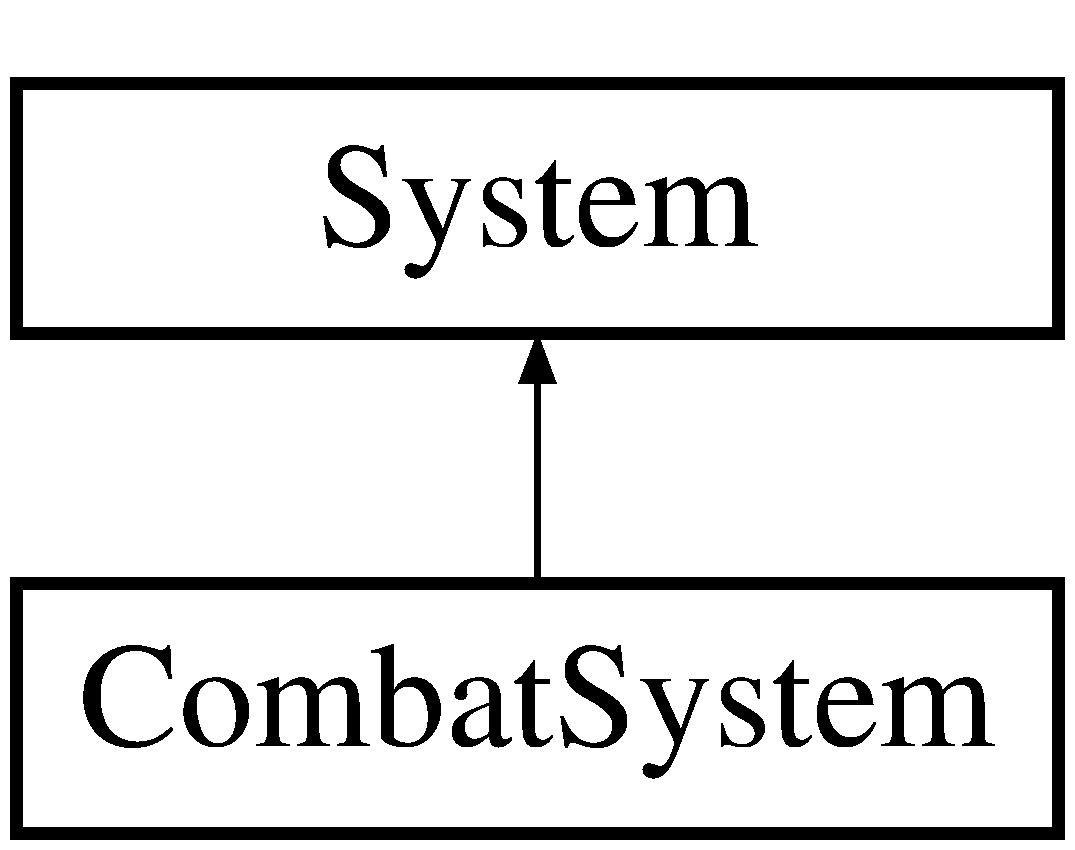
\includegraphics[height=2.000000cm]{class_combat_system}
\end{center}
\end{figure}
\subsection*{Public Member Functions}
\begin{DoxyCompactItemize}
\item 
\hyperlink{class_combat_system_ad7d0ab805abdae93ccaa9d09f9d40153}{Combat\+System} (\hyperlink{class_entity_system}{Entity\+System} \&, Ogre\+::\+Scene\+Manager \&, \hyperlink{class_grid_system}{Grid\+System} \&)
\begin{DoxyCompactList}\small\item\em Constructor. \end{DoxyCompactList}\item 
\hyperlink{class_combat_system_ae95bc02a8ac9237e5dca11f56ecefe9e}{$\sim$\+Combat\+System} ()=default
\begin{DoxyCompactList}\small\item\em Destructor. \end{DoxyCompactList}\item 
void \hyperlink{class_combat_system_a2c284a065f150a9fb67dae0f1229db37}{update} (tdt\+::real) override
\begin{DoxyCompactList}\small\item\em Updates all auto attack combat in the game currently in progress. \end{DoxyCompactList}\item 
bool \hyperlink{class_combat_system_a9e4c1c2747bd800a6766a59f633c7177}{in\+\_\+sight} (tdt\+::uint, tdt\+::uint) const 
\begin{DoxyCompactList}\small\item\em Returns true if two given entities can see each other, false otherwise. \end{DoxyCompactList}\item 
bool \hyperlink{class_combat_system_ad573eb3a0e7751ffc5a6be31f6443c9f}{in\+\_\+sight\+\_\+wrt\+\_\+\+BB} (tdt\+::uint, tdt\+::uint) const 
\begin{DoxyCompactList}\small\item\em Returns true if two given entities can see each other, false otherwise. \end{DoxyCompactList}\item 
tdt\+::uint \hyperlink{class_combat_system_acc161d46979586d368d28a7ee92b79e8}{get\+\_\+closest\+\_\+entity} (tdt\+::uint, bool=true, bool=false) const 
\begin{DoxyCompactList}\small\item\em Returns the ID of the closest entity (from a given entity\textquotesingle{}s position), Component\+::\+N\+O\+\_\+\+E\+N\+T\+I\+TY otherwise. \end{DoxyCompactList}\item 
tdt\+::uint \hyperlink{class_combat_system_afdb21b7f8f95c609e4c00ae6206ac942}{get\+\_\+closest\+\_\+structure} (tdt\+::uint, bool=true, bool=false) const 
\begin{DoxyCompactList}\small\item\em Returns the ID of the closest structure (from a given entity\textquotesingle{}s position), Component\+::\+N\+O\+\_\+\+E\+N\+T\+I\+TY otherwise. \end{DoxyCompactList}\item 
tdt\+::uint \hyperlink{class_combat_system_a1a2d9e90b900331d004d10e2d6e39329}{get\+\_\+closest\+\_\+entity\+\_\+thats\+\_\+not} (tdt\+::uint, tdt\+::uint, bool=true, bool=false) const 
\begin{DoxyCompactList}\small\item\em Returns the ID of the closest entity (from a given entity\textquotesingle{}s position) ignoring a given entity, Component\+::\+N\+O\+\_\+\+E\+N\+T\+I\+TY otherwise. \end{DoxyCompactList}\item 
tdt\+::uint \hyperlink{class_combat_system_a6776c78cfda064865b66b60f1a0bd6e1}{get\+\_\+closest\+\_\+gold\+\_\+deposit} (tdt\+::uint, bool=false) const 
\begin{DoxyCompactList}\small\item\em Returns the ID of the closest gold deposit (entity with both structure and gold components). \end{DoxyCompactList}\item 
tdt\+::uint \hyperlink{class_combat_system_a9b467406db2dae24848078435a78c95c}{get\+\_\+closest\+\_\+gold\+\_\+vault} (tdt\+::uint, bool=false, bool=false) const 
\begin{DoxyCompactList}\small\item\em Returns the ID of the closest gold vault that can store player\textquotesingle{}s gold. \end{DoxyCompactList}\item 
{\footnotesize template$<$typename C\+O\+NT , typename C\+O\+ND $>$ }\\tdt\+::uint \hyperlink{class_combat_system_a94734d18facf7af7172fca0d22dcad49}{get\+\_\+closest\+\_\+entity} (tdt\+::uint id, C\+O\+ND \&condition, bool only\+\_\+sight=true) const 
\begin{DoxyCompactList}\small\item\em Returns the ID of the closest entity that has a given component, meets a given condition and is accessible. \end{DoxyCompactList}\item 
{\footnotesize template$<$typename C\+O\+NT , typename C\+O\+ND , typename E\+F\+F\+E\+CT $>$ }\\void \hyperlink{class_combat_system_a7003f0a13c90284528508282c6ac81f9}{apply\+\_\+effect\+\_\+to\+\_\+entities\+\_\+in\+\_\+range} (tdt\+::uint id, C\+O\+ND \&condition, E\+F\+F\+E\+CT \&effect, tdt\+::real range)
\begin{DoxyCompactList}\small\item\em Applies a given effect (functor given by the template argument E\+F\+F\+E\+CT) to all entities conforming the condition (functor given by the template argument C\+O\+ND) in a given range from a given entity. \end{DoxyCompactList}\item 
void \hyperlink{class_combat_system_a1ea784797f890c7aebeff257624bbea6}{apply\+\_\+heal\+\_\+to\+\_\+entities\+\_\+in\+\_\+range} (tdt\+::uint, tdt\+::real)
\begin{DoxyCompactList}\small\item\em Heals all friendly entities within a given range from a given entity. \end{DoxyCompactList}\item 
void \hyperlink{class_combat_system_a31038240f549621d2ec192b0942e29c5}{apply\+\_\+damage\+\_\+to\+\_\+entities\+\_\+in\+\_\+range} (tdt\+::uint, tdt\+::real, tdt\+::uint, tdt\+::uint)
\begin{DoxyCompactList}\small\item\em Damages all friendly entities within a given range from a given entity. \end{DoxyCompactList}\item 
void \hyperlink{class_combat_system_ae64eaa3c5a01037a6b1ea9db3bb93747}{apply\+\_\+slow\+\_\+to\+\_\+entities\+\_\+in\+\_\+range} (tdt\+::uint, tdt\+::real, tdt\+::real)
\begin{DoxyCompactList}\small\item\em Slows all enemy entities within a given range from a given entity for a given time period. \end{DoxyCompactList}\item 
void \hyperlink{class_combat_system_a3cd665daca2c1c49ca0788d97f5d2c8f}{apply\+\_\+freeze\+\_\+to\+\_\+entities\+\_\+in\+\_\+range} (tdt\+::uint, tdt\+::real, tdt\+::real)
\begin{DoxyCompactList}\small\item\em Freezes all enemy entities within a given range from a given entity for a given time period. \end{DoxyCompactList}\item 
void \hyperlink{class_combat_system_a99deeb9898f08379e2ff0e1471428a1f}{apply\+\_\+slow\+\_\+to} (tdt\+::uint, tdt\+::real)
\begin{DoxyCompactList}\small\item\em Slows a given entity for a given time period. \end{DoxyCompactList}\item 
void \hyperlink{class_combat_system_a67c67143f6d96a5f0947627b7c355dfe}{apply\+\_\+freeze\+\_\+to} (tdt\+::uint, tdt\+::real)
\begin{DoxyCompactList}\small\item\em Freezes a given entity for a given time period. \end{DoxyCompactList}\item 
void \hyperlink{class_combat_system_aa1dcd9b7fa26a536bfee3cb7a2b90d3a}{run\+\_\+away\+\_\+from} (tdt\+::uint, tdt\+::uint, tdt\+::uint)
\begin{DoxyCompactList}\small\item\em Tries to find a path used by an entity to run away from another entity. \end{DoxyCompactList}\item 
void \hyperlink{class_combat_system_a3345cf86852bee674fdd61b8c82001c7}{set\+\_\+max\+\_\+run\+\_\+away\+\_\+attempts} (tdt\+::uint)
\begin{DoxyCompactList}\small\item\em Sets the maximum amount of pathfinding attempts for running away. \end{DoxyCompactList}\item 
tdt\+::uint \hyperlink{class_combat_system_a6144440bbf7eeced81444326e42e6645}{get\+\_\+max\+\_\+run\+\_\+away\+\_\+attempts} ()
\begin{DoxyCompactList}\small\item\em Returns the maximum amount of pathfinding attempts for running away. \end{DoxyCompactList}\item 
bool \hyperlink{class_combat_system_a9ec58d96936e66225997d9d7df7717d0}{enemy\+\_\+in\+\_\+range} (tdt\+::uint)
\begin{DoxyCompactList}\small\item\em Returns true if an enemy is in range from a given entity, false otherwise. \end{DoxyCompactList}\item 
{\footnotesize template$<$$>$ }\\const std\+::map$<$ tdt\+::uint, A\+L\+L\+\_\+\+C\+O\+M\+P\+O\+N\+E\+N\+TS $>$ \& \hyperlink{class_combat_system_a6e001848f89439467e08c8d1fcd10e2b}{get\+\_\+container} () const 
\begin{DoxyCompactList}\small\item\em Specific case of the get\+\_\+container method, which returns the map containing $<$ID, component bitset$>$ map containing all entities. \end{DoxyCompactList}\end{DoxyCompactItemize}
\subsection*{Private Member Functions}
\begin{DoxyCompactItemize}
\item 
{\footnotesize template$<$typename C\+O\+MP $>$ }\\const std\+::map$<$ tdt\+::uint, C\+O\+MP $>$ \& \hyperlink{class_combat_system_a009e7e33b36a38e037662cc662b57774}{get\+\_\+container} () const 
\begin{DoxyCompactList}\small\item\em Retuns a map containing pairs of I\+Ds and components of a given type, use the type A\+L\+L\+\_\+\+C\+O\+M\+P\+O\+N\+E\+N\+TS to get the $<$ID, component bitset$>$ container. \end{DoxyCompactList}\item 
void \hyperlink{class_combat_system_a57555ff5cfbf11cabf4dc558c64e265a}{create\+\_\+homing\+\_\+projectile} (tdt\+::uint, \hyperlink{struct_combat_component}{Combat\+Component} \&)
\begin{DoxyCompactList}\small\item\em Creates a new homing projectile at the position of a given entity homing at the entity\textquotesingle{}s current target. \end{DoxyCompactList}\item 
void \hyperlink{class_combat_system_a77244dfa4506f9f88f43cb4a3f938098}{run\+\_\+away\+\_\+from\+\_\+} (tdt\+::uint, tdt\+::uint, tdt\+::uint)
\begin{DoxyCompactList}\small\item\em Tries to find a path used by an entity to run away from another entity. \end{DoxyCompactList}\end{DoxyCompactItemize}
\subsection*{Private Attributes}
\begin{DoxyCompactItemize}
\item 
\hyperlink{class_entity_system}{Entity\+System} \& \hyperlink{class_combat_system_a801a051bdd230885b786fcc7b2dad9af}{entities\+\_\+}
\begin{DoxyCompactList}\small\item\em Reference to the game\textquotesingle{}s entity system (component retrieval). \end{DoxyCompactList}\item 
Ogre\+::\+Ray\+Scene\+Query \& \hyperlink{class_combat_system_a03b947e997e7138738daf26f48eac7dd}{ray\+\_\+query\+\_\+}
\begin{DoxyCompactList}\small\item\em Reference to the ray cast used to check if two entities can see each other. \end{DoxyCompactList}\item 
\hyperlink{class_grid_system}{Grid\+System} \& \hyperlink{class_combat_system_a90e8e6bb234cb358f676101f8da2daaf}{grid\+\_\+}
\begin{DoxyCompactList}\small\item\em Used to check if an entity is accessible. \end{DoxyCompactList}\item 
\hyperlink{class_ray_caster}{Ray\+Caster} \hyperlink{class_combat_system_aefac99884a4c7fa895f09dd484a3bd15}{ray\+\_\+caster\+\_\+}
\begin{DoxyCompactList}\small\item\em Used for polygon precise line of sight checking. \end{DoxyCompactList}\item 
tdt\+::uint \hyperlink{class_combat_system_a1b68f04d3aee2673466cc57701d8e2e1}{max\+\_\+run\+\_\+away\+\_\+attempts\+\_\+} \{10\}
\begin{DoxyCompactList}\small\item\em Maximum amount of pathfindings performed when running away from an enemy. \end{DoxyCompactList}\item 
std\+::queue$<$ std\+::tuple$<$ tdt\+::uint, tdt\+::uint, tdt\+::uint $>$ $>$ \hyperlink{class_combat_system_aafe37a8f7fa29174c136c747a3d7ee54}{run\+\_\+away\+\_\+queue\+\_\+}
\begin{DoxyCompactList}\small\item\em Used to distribute run away pathfindings over frames (otherwise something like a meteor falling on a big group of entities would freeze the game until all run away pathfindings are done.) \end{DoxyCompactList}\end{DoxyCompactItemize}


\subsection{Detailed Description}
Manages auto attack melee and ranged combat, special melee and ranged attacks will be both handled by the spellcasting system. 

Definition at line 28 of file Combat\+System.\+hpp.



\subsection{Constructor \& Destructor Documentation}
\index{Combat\+System@{Combat\+System}!Combat\+System@{Combat\+System}}
\index{Combat\+System@{Combat\+System}!Combat\+System@{Combat\+System}}
\subsubsection[{\texorpdfstring{Combat\+System(\+Entity\+System \&, Ogre\+::\+Scene\+Manager \&, Grid\+System \&)}{CombatSystem(EntitySystem &, Ogre::SceneManager &, GridSystem &)}}]{\setlength{\rightskip}{0pt plus 5cm}Combat\+System\+::\+Combat\+System (
\begin{DoxyParamCaption}
\item[{{\bf Entity\+System} \&}]{ents, }
\item[{Ogre\+::\+Scene\+Manager \&}]{scene, }
\item[{{\bf Grid\+System} \&}]{grid}
\end{DoxyParamCaption}
)}\hypertarget{class_combat_system_ad7d0ab805abdae93ccaa9d09f9d40153}{}\label{class_combat_system_ad7d0ab805abdae93ccaa9d09f9d40153}


Constructor. 


\begin{DoxyParams}{Parameters}
{\em Reference} & to the game\textquotesingle{}s entity system (component retrieval). \\
\hline
{\em Reference} & to the main scene manager (ray casting). \\
\hline
{\em Reference} & to the game\textquotesingle{}s grid system (accessibility). \\
\hline
\end{DoxyParams}


Definition at line 11 of file Combat\+System.\+cpp.

\index{Combat\+System@{Combat\+System}!````~Combat\+System@{$\sim$\+Combat\+System}}
\index{````~Combat\+System@{$\sim$\+Combat\+System}!Combat\+System@{Combat\+System}}
\subsubsection[{\texorpdfstring{$\sim$\+Combat\+System()=default}{~CombatSystem()=default}}]{\setlength{\rightskip}{0pt plus 5cm}Combat\+System\+::$\sim$\+Combat\+System (
\begin{DoxyParamCaption}
{}
\end{DoxyParamCaption}
)\hspace{0.3cm}{\ttfamily [default]}}\hypertarget{class_combat_system_ae95bc02a8ac9237e5dca11f56ecefe9e}{}\label{class_combat_system_ae95bc02a8ac9237e5dca11f56ecefe9e}


Destructor. 



\subsection{Member Function Documentation}
\index{Combat\+System@{Combat\+System}!apply\+\_\+damage\+\_\+to\+\_\+entities\+\_\+in\+\_\+range@{apply\+\_\+damage\+\_\+to\+\_\+entities\+\_\+in\+\_\+range}}
\index{apply\+\_\+damage\+\_\+to\+\_\+entities\+\_\+in\+\_\+range@{apply\+\_\+damage\+\_\+to\+\_\+entities\+\_\+in\+\_\+range}!Combat\+System@{Combat\+System}}
\subsubsection[{\texorpdfstring{apply\+\_\+damage\+\_\+to\+\_\+entities\+\_\+in\+\_\+range(tdt\+::uint, tdt\+::real, tdt\+::uint, tdt\+::uint)}{apply_damage_to_entities_in_range(tdt::uint, tdt::real, tdt::uint, tdt::uint)}}]{\setlength{\rightskip}{0pt plus 5cm}void Combat\+System\+::apply\+\_\+damage\+\_\+to\+\_\+entities\+\_\+in\+\_\+range (
\begin{DoxyParamCaption}
\item[{tdt\+::uint}]{id, }
\item[{tdt\+::real}]{range, }
\item[{tdt\+::uint}]{min, }
\item[{tdt\+::uint}]{max}
\end{DoxyParamCaption}
)}\hypertarget{class_combat_system_a31038240f549621d2ec192b0942e29c5}{}\label{class_combat_system_a31038240f549621d2ec192b0942e29c5}


Damages all friendly entities within a given range from a given entity. 


\begin{DoxyParams}{Parameters}
{\em ID} & of the entity. \\
\hline
{\em The} & range. \\
\hline
{\em Minimal} & damage value. \\
\hline
{\em Maximal} & damage value. \\
\hline
\end{DoxyParams}


Definition at line 268 of file Combat\+System.\+cpp.

\index{Combat\+System@{Combat\+System}!apply\+\_\+effect\+\_\+to\+\_\+entities\+\_\+in\+\_\+range@{apply\+\_\+effect\+\_\+to\+\_\+entities\+\_\+in\+\_\+range}}
\index{apply\+\_\+effect\+\_\+to\+\_\+entities\+\_\+in\+\_\+range@{apply\+\_\+effect\+\_\+to\+\_\+entities\+\_\+in\+\_\+range}!Combat\+System@{Combat\+System}}
\subsubsection[{\texorpdfstring{apply\+\_\+effect\+\_\+to\+\_\+entities\+\_\+in\+\_\+range(tdt\+::uint id, C\+O\+N\+D \&condition, E\+F\+F\+E\+C\+T \&effect, tdt\+::real range)}{apply_effect_to_entities_in_range(tdt::uint id, COND &condition, EFFECT &effect, tdt::real range)}}]{\setlength{\rightskip}{0pt plus 5cm}template$<$typename C\+O\+NT , typename C\+O\+ND , typename E\+F\+F\+E\+CT $>$ void Combat\+System\+::apply\+\_\+effect\+\_\+to\+\_\+entities\+\_\+in\+\_\+range (
\begin{DoxyParamCaption}
\item[{tdt\+::uint}]{id, }
\item[{C\+O\+ND \&}]{condition, }
\item[{E\+F\+F\+E\+CT \&}]{effect, }
\item[{tdt\+::real}]{range}
\end{DoxyParamCaption}
)\hspace{0.3cm}{\ttfamily [inline]}}\hypertarget{class_combat_system_a7003f0a13c90284528508282c6ac81f9}{}\label{class_combat_system_a7003f0a13c90284528508282c6ac81f9}


Applies a given effect (functor given by the template argument E\+F\+F\+E\+CT) to all entities conforming the condition (functor given by the template argument C\+O\+ND) in a given range from a given entity. 


\begin{DoxyParams}{Parameters}
{\em ID} & of the entity. \\
\hline
{\em Instance} & of the condition functor. \\
\hline
{\em Instance} & of the effect functor. \\
\hline
{\em The} & radius. \\
\hline
\end{DoxyParams}
\begin{DoxyNote}{Note}
The explicit template specialization determines over which component container this method will iterate, use a component name for a specific components only or A\+L\+L\+\_\+\+C\+O\+M\+P\+O\+N\+E\+N\+TS for the component bitset map (which allows to iterate over all entitites regardless of their components). 
\end{DoxyNote}


Definition at line 170 of file Combat\+System.\+hpp.

\index{Combat\+System@{Combat\+System}!apply\+\_\+freeze\+\_\+to@{apply\+\_\+freeze\+\_\+to}}
\index{apply\+\_\+freeze\+\_\+to@{apply\+\_\+freeze\+\_\+to}!Combat\+System@{Combat\+System}}
\subsubsection[{\texorpdfstring{apply\+\_\+freeze\+\_\+to(tdt\+::uint, tdt\+::real)}{apply_freeze_to(tdt::uint, tdt::real)}}]{\setlength{\rightskip}{0pt plus 5cm}void Combat\+System\+::apply\+\_\+freeze\+\_\+to (
\begin{DoxyParamCaption}
\item[{tdt\+::uint}]{id, }
\item[{tdt\+::real}]{time}
\end{DoxyParamCaption}
)}\hypertarget{class_combat_system_a67c67143f6d96a5f0947627b7c355dfe}{}\label{class_combat_system_a67c67143f6d96a5f0947627b7c355dfe}


Freezes a given entity for a given time period. 


\begin{DoxyParams}{Parameters}
{\em ID} & of the entity. \\
\hline
{\em The} & time period for which the freeze is active. \\
\hline
\end{DoxyParams}


Definition at line 295 of file Combat\+System.\+cpp.

\index{Combat\+System@{Combat\+System}!apply\+\_\+freeze\+\_\+to\+\_\+entities\+\_\+in\+\_\+range@{apply\+\_\+freeze\+\_\+to\+\_\+entities\+\_\+in\+\_\+range}}
\index{apply\+\_\+freeze\+\_\+to\+\_\+entities\+\_\+in\+\_\+range@{apply\+\_\+freeze\+\_\+to\+\_\+entities\+\_\+in\+\_\+range}!Combat\+System@{Combat\+System}}
\subsubsection[{\texorpdfstring{apply\+\_\+freeze\+\_\+to\+\_\+entities\+\_\+in\+\_\+range(tdt\+::uint, tdt\+::real, tdt\+::real)}{apply_freeze_to_entities_in_range(tdt::uint, tdt::real, tdt::real)}}]{\setlength{\rightskip}{0pt plus 5cm}void Combat\+System\+::apply\+\_\+freeze\+\_\+to\+\_\+entities\+\_\+in\+\_\+range (
\begin{DoxyParamCaption}
\item[{tdt\+::uint}]{id, }
\item[{tdt\+::real}]{range, }
\item[{tdt\+::real}]{time}
\end{DoxyParamCaption}
)}\hypertarget{class_combat_system_a3cd665daca2c1c49ca0788d97f5d2c8f}{}\label{class_combat_system_a3cd665daca2c1c49ca0788d97f5d2c8f}


Freezes all enemy entities within a given range from a given entity for a given time period. 


\begin{DoxyParams}{Parameters}
{\em ID} & of the entity. \\
\hline
{\em The} & range. \\
\hline
{\em The} & time period for which the freeze is active. \\
\hline
\end{DoxyParams}


Definition at line 282 of file Combat\+System.\+cpp.

\index{Combat\+System@{Combat\+System}!apply\+\_\+heal\+\_\+to\+\_\+entities\+\_\+in\+\_\+range@{apply\+\_\+heal\+\_\+to\+\_\+entities\+\_\+in\+\_\+range}}
\index{apply\+\_\+heal\+\_\+to\+\_\+entities\+\_\+in\+\_\+range@{apply\+\_\+heal\+\_\+to\+\_\+entities\+\_\+in\+\_\+range}!Combat\+System@{Combat\+System}}
\subsubsection[{\texorpdfstring{apply\+\_\+heal\+\_\+to\+\_\+entities\+\_\+in\+\_\+range(tdt\+::uint, tdt\+::real)}{apply_heal_to_entities_in_range(tdt::uint, tdt::real)}}]{\setlength{\rightskip}{0pt plus 5cm}void Combat\+System\+::apply\+\_\+heal\+\_\+to\+\_\+entities\+\_\+in\+\_\+range (
\begin{DoxyParamCaption}
\item[{tdt\+::uint}]{id, }
\item[{tdt\+::real}]{range}
\end{DoxyParamCaption}
)}\hypertarget{class_combat_system_a1ea784797f890c7aebeff257624bbea6}{}\label{class_combat_system_a1ea784797f890c7aebeff257624bbea6}


Heals all friendly entities within a given range from a given entity. 


\begin{DoxyParams}{Parameters}
{\em ID} & of the entity. \\
\hline
{\em The} & range. \\
\hline
\end{DoxyParams}


Definition at line 261 of file Combat\+System.\+cpp.

\index{Combat\+System@{Combat\+System}!apply\+\_\+slow\+\_\+to@{apply\+\_\+slow\+\_\+to}}
\index{apply\+\_\+slow\+\_\+to@{apply\+\_\+slow\+\_\+to}!Combat\+System@{Combat\+System}}
\subsubsection[{\texorpdfstring{apply\+\_\+slow\+\_\+to(tdt\+::uint, tdt\+::real)}{apply_slow_to(tdt::uint, tdt::real)}}]{\setlength{\rightskip}{0pt plus 5cm}void Combat\+System\+::apply\+\_\+slow\+\_\+to (
\begin{DoxyParamCaption}
\item[{tdt\+::uint}]{id, }
\item[{tdt\+::real}]{time}
\end{DoxyParamCaption}
)}\hypertarget{class_combat_system_a99deeb9898f08379e2ff0e1471428a1f}{}\label{class_combat_system_a99deeb9898f08379e2ff0e1471428a1f}


Slows a given entity for a given time period. 


\begin{DoxyParams}{Parameters}
{\em ID} & of the entity. \\
\hline
{\em The} & time period for which the freeze is active. \\
\hline
\end{DoxyParams}


Definition at line 289 of file Combat\+System.\+cpp.

\index{Combat\+System@{Combat\+System}!apply\+\_\+slow\+\_\+to\+\_\+entities\+\_\+in\+\_\+range@{apply\+\_\+slow\+\_\+to\+\_\+entities\+\_\+in\+\_\+range}}
\index{apply\+\_\+slow\+\_\+to\+\_\+entities\+\_\+in\+\_\+range@{apply\+\_\+slow\+\_\+to\+\_\+entities\+\_\+in\+\_\+range}!Combat\+System@{Combat\+System}}
\subsubsection[{\texorpdfstring{apply\+\_\+slow\+\_\+to\+\_\+entities\+\_\+in\+\_\+range(tdt\+::uint, tdt\+::real, tdt\+::real)}{apply_slow_to_entities_in_range(tdt::uint, tdt::real, tdt::real)}}]{\setlength{\rightskip}{0pt plus 5cm}void Combat\+System\+::apply\+\_\+slow\+\_\+to\+\_\+entities\+\_\+in\+\_\+range (
\begin{DoxyParamCaption}
\item[{tdt\+::uint}]{id, }
\item[{tdt\+::real}]{range, }
\item[{tdt\+::real}]{time}
\end{DoxyParamCaption}
)}\hypertarget{class_combat_system_ae64eaa3c5a01037a6b1ea9db3bb93747}{}\label{class_combat_system_ae64eaa3c5a01037a6b1ea9db3bb93747}


Slows all enemy entities within a given range from a given entity for a given time period. 


\begin{DoxyParams}{Parameters}
{\em ID} & of the entity. \\
\hline
{\em The} & range. \\
\hline
{\em The} & time period for which the slow is active. \\
\hline
\end{DoxyParams}


Definition at line 275 of file Combat\+System.\+cpp.

\index{Combat\+System@{Combat\+System}!create\+\_\+homing\+\_\+projectile@{create\+\_\+homing\+\_\+projectile}}
\index{create\+\_\+homing\+\_\+projectile@{create\+\_\+homing\+\_\+projectile}!Combat\+System@{Combat\+System}}
\subsubsection[{\texorpdfstring{create\+\_\+homing\+\_\+projectile(tdt\+::uint, Combat\+Component \&)}{create_homing_projectile(tdt::uint, CombatComponent &)}}]{\setlength{\rightskip}{0pt plus 5cm}void Combat\+System\+::create\+\_\+homing\+\_\+projectile (
\begin{DoxyParamCaption}
\item[{tdt\+::uint}]{caster, }
\item[{{\bf Combat\+Component} \&}]{combat}
\end{DoxyParamCaption}
)\hspace{0.3cm}{\ttfamily [private]}}\hypertarget{class_combat_system_a57555ff5cfbf11cabf4dc558c64e265a}{}\label{class_combat_system_a57555ff5cfbf11cabf4dc558c64e265a}


Creates a new homing projectile at the position of a given entity homing at the entity\textquotesingle{}s current target. 


\begin{DoxyParams}{Parameters}
{\em ID} & of the caster entity. \\
\hline
{\em Reference} & to the caster entity\textquotesingle{}s combat component. \\
\hline
\end{DoxyParams}


Definition at line 387 of file Combat\+System.\+cpp.

\index{Combat\+System@{Combat\+System}!enemy\+\_\+in\+\_\+range@{enemy\+\_\+in\+\_\+range}}
\index{enemy\+\_\+in\+\_\+range@{enemy\+\_\+in\+\_\+range}!Combat\+System@{Combat\+System}}
\subsubsection[{\texorpdfstring{enemy\+\_\+in\+\_\+range(tdt\+::uint)}{enemy_in_range(tdt::uint)}}]{\setlength{\rightskip}{0pt plus 5cm}bool Combat\+System\+::enemy\+\_\+in\+\_\+range (
\begin{DoxyParamCaption}
\item[{tdt\+::uint}]{id}
\end{DoxyParamCaption}
)}\hypertarget{class_combat_system_a9ec58d96936e66225997d9d7df7717d0}{}\label{class_combat_system_a9ec58d96936e66225997d9d7df7717d0}


Returns true if an enemy is in range from a given entity, false otherwise. 


\begin{DoxyParams}{Parameters}
{\em ID} & of the entity. \\
\hline
\end{DoxyParams}


Definition at line 356 of file Combat\+System.\+cpp.

\index{Combat\+System@{Combat\+System}!get\+\_\+closest\+\_\+entity@{get\+\_\+closest\+\_\+entity}}
\index{get\+\_\+closest\+\_\+entity@{get\+\_\+closest\+\_\+entity}!Combat\+System@{Combat\+System}}
\subsubsection[{\texorpdfstring{get\+\_\+closest\+\_\+entity(tdt\+::uint, bool=true, bool=false) const }{get_closest_entity(tdt::uint, bool=true, bool=false) const }}]{\setlength{\rightskip}{0pt plus 5cm}std\+::size\+\_\+t Combat\+System\+::get\+\_\+closest\+\_\+entity (
\begin{DoxyParamCaption}
\item[{tdt\+::uint}]{id, }
\item[{bool}]{only\+\_\+sight = {\ttfamily true}, }
\item[{bool}]{friendly = {\ttfamily false}}
\end{DoxyParamCaption}
) const}\hypertarget{class_combat_system_acc161d46979586d368d28a7ee92b79e8}{}\label{class_combat_system_acc161d46979586d368d28a7ee92b79e8}


Returns the ID of the closest entity (from a given entity\textquotesingle{}s position), Component\+::\+N\+O\+\_\+\+E\+N\+T\+I\+TY otherwise. 


\begin{DoxyParams}{Parameters}
{\em ID} & of the entity from whose position the search is performed. \\
\hline
{\em If} & true, will return only entities in sight. \\
\hline
{\em If} & true, will return only friendly entities (enemies otherwise). \\
\hline
\end{DoxyParams}


Definition at line 208 of file Combat\+System.\+cpp.

\index{Combat\+System@{Combat\+System}!get\+\_\+closest\+\_\+entity@{get\+\_\+closest\+\_\+entity}}
\index{get\+\_\+closest\+\_\+entity@{get\+\_\+closest\+\_\+entity}!Combat\+System@{Combat\+System}}
\subsubsection[{\texorpdfstring{get\+\_\+closest\+\_\+entity(tdt\+::uint id, C\+O\+N\+D \&condition, bool only\+\_\+sight=true) const }{get_closest_entity(tdt::uint id, COND &condition, bool only_sight=true) const }}]{\setlength{\rightskip}{0pt plus 5cm}template$<$typename C\+O\+NT , typename C\+O\+ND $>$ tdt\+::uint Combat\+System\+::get\+\_\+closest\+\_\+entity (
\begin{DoxyParamCaption}
\item[{tdt\+::uint}]{id, }
\item[{C\+O\+ND \&}]{condition, }
\item[{bool}]{only\+\_\+sight = {\ttfamily true}}
\end{DoxyParamCaption}
) const\hspace{0.3cm}{\ttfamily [inline]}}\hypertarget{class_combat_system_a94734d18facf7af7172fca0d22dcad49}{}\label{class_combat_system_a94734d18facf7af7172fca0d22dcad49}


Returns the ID of the closest entity that has a given component, meets a given condition and is accessible. 


\begin{DoxyParams}{Parameters}
{\em ID} & of the entity that is searching. \\
\hline
{\em Functor} & representing the condition. \\
\hline
{\em If} & true, only entities in sight get checked. \\
\hline
\end{DoxyParams}
\begin{DoxyNote}{Note}
The explicit template specialization determines over which component container this method will iterate, use a component name for a specific components only or A\+L\+L\+\_\+\+C\+O\+M\+P\+O\+N\+E\+N\+TS for the component bitset map (which allows to iterate over all entitites regardless of their components). 
\end{DoxyNote}


Definition at line 128 of file Combat\+System.\+hpp.

\index{Combat\+System@{Combat\+System}!get\+\_\+closest\+\_\+entity\+\_\+thats\+\_\+not@{get\+\_\+closest\+\_\+entity\+\_\+thats\+\_\+not}}
\index{get\+\_\+closest\+\_\+entity\+\_\+thats\+\_\+not@{get\+\_\+closest\+\_\+entity\+\_\+thats\+\_\+not}!Combat\+System@{Combat\+System}}
\subsubsection[{\texorpdfstring{get\+\_\+closest\+\_\+entity\+\_\+thats\+\_\+not(tdt\+::uint, tdt\+::uint, bool=true, bool=false) const }{get_closest_entity_thats_not(tdt::uint, tdt::uint, bool=true, bool=false) const }}]{\setlength{\rightskip}{0pt plus 5cm}std\+::size\+\_\+t Combat\+System\+::get\+\_\+closest\+\_\+entity\+\_\+thats\+\_\+not (
\begin{DoxyParamCaption}
\item[{tdt\+::uint}]{id, }
\item[{tdt\+::uint}]{ignored, }
\item[{bool}]{only\+\_\+sight = {\ttfamily true}, }
\item[{bool}]{friendly = {\ttfamily false}}
\end{DoxyParamCaption}
) const}\hypertarget{class_combat_system_a1a2d9e90b900331d004d10e2d6e39329}{}\label{class_combat_system_a1a2d9e90b900331d004d10e2d6e39329}


Returns the ID of the closest entity (from a given entity\textquotesingle{}s position) ignoring a given entity, Component\+::\+N\+O\+\_\+\+E\+N\+T\+I\+TY otherwise. 


\begin{DoxyParams}{Parameters}
{\em ID} & of the entity from whose position the search is performed. \\
\hline
{\em ID} & of the entity that\textquotesingle{}s ignored in the search. \\
\hline
{\em If} & true, will return only entities in sight. \\
\hline
{\em If} & true, will return only friendly entities (enemies otherwise). \\
\hline
\end{DoxyParams}


Definition at line 224 of file Combat\+System.\+cpp.

\index{Combat\+System@{Combat\+System}!get\+\_\+closest\+\_\+gold\+\_\+deposit@{get\+\_\+closest\+\_\+gold\+\_\+deposit}}
\index{get\+\_\+closest\+\_\+gold\+\_\+deposit@{get\+\_\+closest\+\_\+gold\+\_\+deposit}!Combat\+System@{Combat\+System}}
\subsubsection[{\texorpdfstring{get\+\_\+closest\+\_\+gold\+\_\+deposit(tdt\+::uint, bool=false) const }{get_closest_gold_deposit(tdt::uint, bool=false) const }}]{\setlength{\rightskip}{0pt plus 5cm}std\+::size\+\_\+t Combat\+System\+::get\+\_\+closest\+\_\+gold\+\_\+deposit (
\begin{DoxyParamCaption}
\item[{tdt\+::uint}]{id, }
\item[{bool}]{only\+\_\+sight = {\ttfamily false}}
\end{DoxyParamCaption}
) const}\hypertarget{class_combat_system_a6776c78cfda064865b66b60f1a0bd6e1}{}\label{class_combat_system_a6776c78cfda064865b66b60f1a0bd6e1}


Returns the ID of the closest gold deposit (entity with both structure and gold components). 


\begin{DoxyParams}{Parameters}
{\em ID} & of the entity that looks for the gold deposit. \\
\hline
{\em If} & true, only deposits in sight will be checked. \\
\hline
\end{DoxyParams}


Definition at line 238 of file Combat\+System.\+cpp.

\index{Combat\+System@{Combat\+System}!get\+\_\+closest\+\_\+gold\+\_\+vault@{get\+\_\+closest\+\_\+gold\+\_\+vault}}
\index{get\+\_\+closest\+\_\+gold\+\_\+vault@{get\+\_\+closest\+\_\+gold\+\_\+vault}!Combat\+System@{Combat\+System}}
\subsubsection[{\texorpdfstring{get\+\_\+closest\+\_\+gold\+\_\+vault(tdt\+::uint, bool=false, bool=false) const }{get_closest_gold_vault(tdt::uint, bool=false, bool=false) const }}]{\setlength{\rightskip}{0pt plus 5cm}std\+::size\+\_\+t Combat\+System\+::get\+\_\+closest\+\_\+gold\+\_\+vault (
\begin{DoxyParamCaption}
\item[{tdt\+::uint}]{id, }
\item[{bool}]{only\+\_\+sight = {\ttfamily false}, }
\item[{bool}]{only\+\_\+free = {\ttfamily false}}
\end{DoxyParamCaption}
) const}\hypertarget{class_combat_system_a9b467406db2dae24848078435a78c95c}{}\label{class_combat_system_a9b467406db2dae24848078435a78c95c}


Returns the ID of the closest gold vault that can store player\textquotesingle{}s gold. 


\begin{DoxyParams}{Parameters}
{\em ID} & of the entity that looks for the gold vault. \\
\hline
{\em If} & true, only vaults in sight will be checked. \\
\hline
{\em If} & true, only vaults that have free space for more gold will be checked. \\
\hline
\end{DoxyParams}


Definition at line 247 of file Combat\+System.\+cpp.

\index{Combat\+System@{Combat\+System}!get\+\_\+closest\+\_\+structure@{get\+\_\+closest\+\_\+structure}}
\index{get\+\_\+closest\+\_\+structure@{get\+\_\+closest\+\_\+structure}!Combat\+System@{Combat\+System}}
\subsubsection[{\texorpdfstring{get\+\_\+closest\+\_\+structure(tdt\+::uint, bool=true, bool=false) const }{get_closest_structure(tdt::uint, bool=true, bool=false) const }}]{\setlength{\rightskip}{0pt plus 5cm}std\+::size\+\_\+t Combat\+System\+::get\+\_\+closest\+\_\+structure (
\begin{DoxyParamCaption}
\item[{tdt\+::uint}]{id, }
\item[{bool}]{only\+\_\+sight = {\ttfamily true}, }
\item[{bool}]{friendly = {\ttfamily false}}
\end{DoxyParamCaption}
) const}\hypertarget{class_combat_system_afdb21b7f8f95c609e4c00ae6206ac942}{}\label{class_combat_system_afdb21b7f8f95c609e4c00ae6206ac942}


Returns the ID of the closest structure (from a given entity\textquotesingle{}s position), Component\+::\+N\+O\+\_\+\+E\+N\+T\+I\+TY otherwise. 


\begin{DoxyParams}{Parameters}
{\em ID} & of the entity from whose position the search is performed. \\
\hline
{\em If} & true, will return only structures in sight. \\
\hline
{\em If} & true, will return friendly structures (enemies otherwise). \\
\hline
\end{DoxyParams}


Definition at line 216 of file Combat\+System.\+cpp.

\index{Combat\+System@{Combat\+System}!get\+\_\+container@{get\+\_\+container}}
\index{get\+\_\+container@{get\+\_\+container}!Combat\+System@{Combat\+System}}
\subsubsection[{\texorpdfstring{get\+\_\+container() const }{get_container() const }}]{\setlength{\rightskip}{0pt plus 5cm}template$<$typename C\+O\+MP $>$ const std\+::map$<$tdt\+::uint, C\+O\+MP$>$\& Combat\+System\+::get\+\_\+container (
\begin{DoxyParamCaption}
{}
\end{DoxyParamCaption}
) const\hspace{0.3cm}{\ttfamily [inline]}, {\ttfamily [private]}}\hypertarget{class_combat_system_a009e7e33b36a38e037662cc662b57774}{}\label{class_combat_system_a009e7e33b36a38e037662cc662b57774}


Retuns a map containing pairs of I\+Ds and components of a given type, use the type A\+L\+L\+\_\+\+C\+O\+M\+P\+O\+N\+E\+N\+TS to get the $<$ID, component bitset$>$ container. 



Definition at line 269 of file Combat\+System.\+hpp.

\index{Combat\+System@{Combat\+System}!get\+\_\+container@{get\+\_\+container}}
\index{get\+\_\+container@{get\+\_\+container}!Combat\+System@{Combat\+System}}
\subsubsection[{\texorpdfstring{get\+\_\+container() const }{get_container() const }}]{\setlength{\rightskip}{0pt plus 5cm}template$<$$>$ const std\+::map$<$tdt\+::uint, A\+L\+L\+\_\+\+C\+O\+M\+P\+O\+N\+E\+N\+TS$>$\& Combat\+System\+::get\+\_\+container (
\begin{DoxyParamCaption}
{}
\end{DoxyParamCaption}
) const\hspace{0.3cm}{\ttfamily [inline]}}\hypertarget{class_combat_system_a6e001848f89439467e08c8d1fcd10e2b}{}\label{class_combat_system_a6e001848f89439467e08c8d1fcd10e2b}


Specific case of the get\+\_\+container method, which returns the map containing $<$ID, component bitset$>$ map containing all entities. 



Definition at line 331 of file Combat\+System.\+hpp.

\index{Combat\+System@{Combat\+System}!get\+\_\+max\+\_\+run\+\_\+away\+\_\+attempts@{get\+\_\+max\+\_\+run\+\_\+away\+\_\+attempts}}
\index{get\+\_\+max\+\_\+run\+\_\+away\+\_\+attempts@{get\+\_\+max\+\_\+run\+\_\+away\+\_\+attempts}!Combat\+System@{Combat\+System}}
\subsubsection[{\texorpdfstring{get\+\_\+max\+\_\+run\+\_\+away\+\_\+attempts()}{get_max_run_away_attempts()}}]{\setlength{\rightskip}{0pt plus 5cm}std\+::size\+\_\+t Combat\+System\+::get\+\_\+max\+\_\+run\+\_\+away\+\_\+attempts (
\begin{DoxyParamCaption}
{}
\end{DoxyParamCaption}
)}\hypertarget{class_combat_system_a6144440bbf7eeced81444326e42e6645}{}\label{class_combat_system_a6144440bbf7eeced81444326e42e6645}


Returns the maximum amount of pathfinding attempts for running away. 



Definition at line 351 of file Combat\+System.\+cpp.

\index{Combat\+System@{Combat\+System}!in\+\_\+sight@{in\+\_\+sight}}
\index{in\+\_\+sight@{in\+\_\+sight}!Combat\+System@{Combat\+System}}
\subsubsection[{\texorpdfstring{in\+\_\+sight(tdt\+::uint, tdt\+::uint) const }{in_sight(tdt::uint, tdt::uint) const }}]{\setlength{\rightskip}{0pt plus 5cm}bool Combat\+System\+::in\+\_\+sight (
\begin{DoxyParamCaption}
\item[{tdt\+::uint}]{ent\+\_\+id, }
\item[{tdt\+::uint}]{target}
\end{DoxyParamCaption}
) const}\hypertarget{class_combat_system_a9e4c1c2747bd800a6766a59f633c7177}{}\label{class_combat_system_a9e4c1c2747bd800a6766a59f633c7177}


Returns true if two given entities can see each other, false otherwise. 

Tests polygons. 
\begin{DoxyParams}{Parameters}
{\em ID} & of the first entity. \\
\hline
{\em ID} & of the second entity. N\+O\+TE\+: Tests only if entities that have query flags of W\+A\+LL or B\+U\+I\+L\+D\+I\+NG are in the way, allows to see through other friendly/enemy/neutral entities. \\
\hline
\end{DoxyParams}


Definition at line 157 of file Combat\+System.\+cpp.

\index{Combat\+System@{Combat\+System}!in\+\_\+sight\+\_\+wrt\+\_\+\+BB@{in\+\_\+sight\+\_\+wrt\+\_\+\+BB}}
\index{in\+\_\+sight\+\_\+wrt\+\_\+\+BB@{in\+\_\+sight\+\_\+wrt\+\_\+\+BB}!Combat\+System@{Combat\+System}}
\subsubsection[{\texorpdfstring{in\+\_\+sight\+\_\+wrt\+\_\+\+B\+B(tdt\+::uint, tdt\+::uint) const }{in_sight_wrt_BB(tdt::uint, tdt::uint) const }}]{\setlength{\rightskip}{0pt plus 5cm}bool Combat\+System\+::in\+\_\+sight\+\_\+wrt\+\_\+\+BB (
\begin{DoxyParamCaption}
\item[{tdt\+::uint}]{ent\+\_\+id, }
\item[{tdt\+::uint}]{target}
\end{DoxyParamCaption}
) const}\hypertarget{class_combat_system_ad573eb3a0e7751ffc5a6be31f6443c9f}{}\label{class_combat_system_ad573eb3a0e7751ffc5a6be31f6443c9f}


Returns true if two given entities can see each other, false otherwise. 

Tests only bounding boxes. 
\begin{DoxyParams}{Parameters}
{\em ID} & of the first entity. \\
\hline
{\em ID} & of the second entity. N\+O\+TE\+: Tests only if entities that have query flags of W\+A\+LL or B\+U\+I\+L\+D\+I\+NG are in the way, allows to see through other friendly/enemy/neutral entities. \\
\hline
\end{DoxyParams}


Definition at line 181 of file Combat\+System.\+cpp.

\index{Combat\+System@{Combat\+System}!run\+\_\+away\+\_\+from@{run\+\_\+away\+\_\+from}}
\index{run\+\_\+away\+\_\+from@{run\+\_\+away\+\_\+from}!Combat\+System@{Combat\+System}}
\subsubsection[{\texorpdfstring{run\+\_\+away\+\_\+from(tdt\+::uint, tdt\+::uint, tdt\+::uint)}{run_away_from(tdt::uint, tdt::uint, tdt::uint)}}]{\setlength{\rightskip}{0pt plus 5cm}void Combat\+System\+::run\+\_\+away\+\_\+from (
\begin{DoxyParamCaption}
\item[{tdt\+::uint}]{id, }
\item[{tdt\+::uint}]{from\+\_\+id, }
\item[{tdt\+::uint}]{min\+\_\+node\+\_\+count}
\end{DoxyParamCaption}
)}\hypertarget{class_combat_system_aa1dcd9b7fa26a536bfee3cb7a2b90d3a}{}\label{class_combat_system_aa1dcd9b7fa26a536bfee3cb7a2b90d3a}


Tries to find a path used by an entity to run away from another entity. 


\begin{DoxyParams}{Parameters}
{\em ID} & of the entity running away. \\
\hline
{\em ID} & of the entity that is ran away from. \\
\hline
{\em Minimal} & amount of nodes the path has to have (will be ignored if the amount of attempts surpasses the maximum amount). \\
\hline
\end{DoxyParams}
\begin{DoxyNote}{Note}
This is just a dummy that enqueues the entity for pathfinding. 
\end{DoxyNote}


Definition at line 346 of file Combat\+System.\+cpp.

\index{Combat\+System@{Combat\+System}!run\+\_\+away\+\_\+from\+\_\+@{run\+\_\+away\+\_\+from\+\_\+}}
\index{run\+\_\+away\+\_\+from\+\_\+@{run\+\_\+away\+\_\+from\+\_\+}!Combat\+System@{Combat\+System}}
\subsubsection[{\texorpdfstring{run\+\_\+away\+\_\+from\+\_\+(tdt\+::uint, tdt\+::uint, tdt\+::uint)}{run_away_from_(tdt::uint, tdt::uint, tdt::uint)}}]{\setlength{\rightskip}{0pt plus 5cm}void Combat\+System\+::run\+\_\+away\+\_\+from\+\_\+ (
\begin{DoxyParamCaption}
\item[{tdt\+::uint}]{id, }
\item[{tdt\+::uint}]{from\+\_\+id, }
\item[{tdt\+::uint}]{min\+\_\+node\+\_\+count}
\end{DoxyParamCaption}
)\hspace{0.3cm}{\ttfamily [private]}}\hypertarget{class_combat_system_a77244dfa4506f9f88f43cb4a3f938098}{}\label{class_combat_system_a77244dfa4506f9f88f43cb4a3f938098}


Tries to find a path used by an entity to run away from another entity. 


\begin{DoxyParams}{Parameters}
{\em ID} & of the entity running away. \\
\hline
{\em ID} & of the entity that is ran away from. \\
\hline
{\em Minimal} & amount of nodes the path has to have (will be ignored if the amount of attempts surpasses the maximum amount). \\
\hline
\end{DoxyParams}
\begin{DoxyNote}{Note}
This is the actual implementation. 
\end{DoxyNote}


Definition at line 301 of file Combat\+System.\+cpp.

\index{Combat\+System@{Combat\+System}!set\+\_\+max\+\_\+run\+\_\+away\+\_\+attempts@{set\+\_\+max\+\_\+run\+\_\+away\+\_\+attempts}}
\index{set\+\_\+max\+\_\+run\+\_\+away\+\_\+attempts@{set\+\_\+max\+\_\+run\+\_\+away\+\_\+attempts}!Combat\+System@{Combat\+System}}
\subsubsection[{\texorpdfstring{set\+\_\+max\+\_\+run\+\_\+away\+\_\+attempts(tdt\+::uint)}{set_max_run_away_attempts(tdt::uint)}}]{\setlength{\rightskip}{0pt plus 5cm}void Combat\+System\+::set\+\_\+max\+\_\+run\+\_\+away\+\_\+attempts (
\begin{DoxyParamCaption}
\item[{tdt\+::uint}]{val}
\end{DoxyParamCaption}
)}\hypertarget{class_combat_system_a3345cf86852bee674fdd61b8c82001c7}{}\label{class_combat_system_a3345cf86852bee674fdd61b8c82001c7}


Sets the maximum amount of pathfinding attempts for running away. 


\begin{DoxyParams}{Parameters}
{\em The} & new maximum amount. \\
\hline
\end{DoxyParams}


Definition at line 341 of file Combat\+System.\+cpp.

\index{Combat\+System@{Combat\+System}!update@{update}}
\index{update@{update}!Combat\+System@{Combat\+System}}
\subsubsection[{\texorpdfstring{update(tdt\+::real) override}{update(tdt::real) override}}]{\setlength{\rightskip}{0pt plus 5cm}void Combat\+System\+::update (
\begin{DoxyParamCaption}
\item[{tdt\+::real}]{delta}
\end{DoxyParamCaption}
)\hspace{0.3cm}{\ttfamily [override]}, {\ttfamily [virtual]}}\hypertarget{class_combat_system_a2c284a065f150a9fb67dae0f1229db37}{}\label{class_combat_system_a2c284a065f150a9fb67dae0f1229db37}


Updates all auto attack combat in the game currently in progress. 


\begin{DoxyParams}{Parameters}
{\em Time} & since the last frame. \\
\hline
\end{DoxyParams}
Check if the target is in range and in sight and if so, attack, otherwise pursue the target if necessary.

Implements \hyperlink{class_system_a6d54c9bd38eb43d620a1451cb0925472}{System}.



Definition at line 19 of file Combat\+System.\+cpp.



\subsection{Member Data Documentation}
\index{Combat\+System@{Combat\+System}!entities\+\_\+@{entities\+\_\+}}
\index{entities\+\_\+@{entities\+\_\+}!Combat\+System@{Combat\+System}}
\subsubsection[{\texorpdfstring{entities\+\_\+}{entities_}}]{\setlength{\rightskip}{0pt plus 5cm}{\bf Entity\+System}\& Combat\+System\+::entities\+\_\+\hspace{0.3cm}{\ttfamily [private]}}\hypertarget{class_combat_system_a801a051bdd230885b786fcc7b2dad9af}{}\label{class_combat_system_a801a051bdd230885b786fcc7b2dad9af}


Reference to the game\textquotesingle{}s entity system (component retrieval). 



Definition at line 296 of file Combat\+System.\+hpp.

\index{Combat\+System@{Combat\+System}!grid\+\_\+@{grid\+\_\+}}
\index{grid\+\_\+@{grid\+\_\+}!Combat\+System@{Combat\+System}}
\subsubsection[{\texorpdfstring{grid\+\_\+}{grid_}}]{\setlength{\rightskip}{0pt plus 5cm}{\bf Grid\+System}\& Combat\+System\+::grid\+\_\+\hspace{0.3cm}{\ttfamily [private]}}\hypertarget{class_combat_system_a90e8e6bb234cb358f676101f8da2daaf}{}\label{class_combat_system_a90e8e6bb234cb358f676101f8da2daaf}


Used to check if an entity is accessible. 



Definition at line 306 of file Combat\+System.\+hpp.

\index{Combat\+System@{Combat\+System}!max\+\_\+run\+\_\+away\+\_\+attempts\+\_\+@{max\+\_\+run\+\_\+away\+\_\+attempts\+\_\+}}
\index{max\+\_\+run\+\_\+away\+\_\+attempts\+\_\+@{max\+\_\+run\+\_\+away\+\_\+attempts\+\_\+}!Combat\+System@{Combat\+System}}
\subsubsection[{\texorpdfstring{max\+\_\+run\+\_\+away\+\_\+attempts\+\_\+}{max_run_away_attempts_}}]{\setlength{\rightskip}{0pt plus 5cm}tdt\+::uint Combat\+System\+::max\+\_\+run\+\_\+away\+\_\+attempts\+\_\+ \{10\}\hspace{0.3cm}{\ttfamily [private]}}\hypertarget{class_combat_system_a1b68f04d3aee2673466cc57701d8e2e1}{}\label{class_combat_system_a1b68f04d3aee2673466cc57701d8e2e1}


Maximum amount of pathfindings performed when running away from an enemy. 



Definition at line 316 of file Combat\+System.\+hpp.

\index{Combat\+System@{Combat\+System}!ray\+\_\+caster\+\_\+@{ray\+\_\+caster\+\_\+}}
\index{ray\+\_\+caster\+\_\+@{ray\+\_\+caster\+\_\+}!Combat\+System@{Combat\+System}}
\subsubsection[{\texorpdfstring{ray\+\_\+caster\+\_\+}{ray_caster_}}]{\setlength{\rightskip}{0pt plus 5cm}{\bf Ray\+Caster} Combat\+System\+::ray\+\_\+caster\+\_\+\hspace{0.3cm}{\ttfamily [private]}}\hypertarget{class_combat_system_aefac99884a4c7fa895f09dd484a3bd15}{}\label{class_combat_system_aefac99884a4c7fa895f09dd484a3bd15}


Used for polygon precise line of sight checking. 



Definition at line 311 of file Combat\+System.\+hpp.

\index{Combat\+System@{Combat\+System}!ray\+\_\+query\+\_\+@{ray\+\_\+query\+\_\+}}
\index{ray\+\_\+query\+\_\+@{ray\+\_\+query\+\_\+}!Combat\+System@{Combat\+System}}
\subsubsection[{\texorpdfstring{ray\+\_\+query\+\_\+}{ray_query_}}]{\setlength{\rightskip}{0pt plus 5cm}Ogre\+::\+Ray\+Scene\+Query\& Combat\+System\+::ray\+\_\+query\+\_\+\hspace{0.3cm}{\ttfamily [private]}}\hypertarget{class_combat_system_a03b947e997e7138738daf26f48eac7dd}{}\label{class_combat_system_a03b947e997e7138738daf26f48eac7dd}


Reference to the ray cast used to check if two entities can see each other. 



Definition at line 301 of file Combat\+System.\+hpp.

\index{Combat\+System@{Combat\+System}!run\+\_\+away\+\_\+queue\+\_\+@{run\+\_\+away\+\_\+queue\+\_\+}}
\index{run\+\_\+away\+\_\+queue\+\_\+@{run\+\_\+away\+\_\+queue\+\_\+}!Combat\+System@{Combat\+System}}
\subsubsection[{\texorpdfstring{run\+\_\+away\+\_\+queue\+\_\+}{run_away_queue_}}]{\setlength{\rightskip}{0pt plus 5cm}std\+::queue$<$std\+::tuple$<$tdt\+::uint, tdt\+::uint, tdt\+::uint$>$ $>$ Combat\+System\+::run\+\_\+away\+\_\+queue\+\_\+\hspace{0.3cm}{\ttfamily [private]}}\hypertarget{class_combat_system_aafe37a8f7fa29174c136c747a3d7ee54}{}\label{class_combat_system_aafe37a8f7fa29174c136c747a3d7ee54}


Used to distribute run away pathfindings over frames (otherwise something like a meteor falling on a big group of entities would freeze the game until all run away pathfindings are done.) 



Definition at line 323 of file Combat\+System.\+hpp.



The documentation for this class was generated from the following files\+:\begin{DoxyCompactItemize}
\item 
systems/Combat\+System.\+hpp\item 
systems/Combat\+System.\+cpp\end{DoxyCompactItemize}

\hypertarget{struct_command_component}{}\section{Command\+Component Struct Reference}
\label{struct_command_component}\index{Command\+Component@{Command\+Component}}


Contains a list of commands an entity can respond to.  




{\ttfamily \#include $<$Components.\+hpp$>$}

\subsection*{Public Member Functions}
\begin{DoxyCompactItemize}
\item 
{\bfseries Command\+Component} (const \hyperlink{struct_command_component}{Command\+Component} \&)=default\hypertarget{struct_command_component_ae20d2b5b01dc704075a7172e186397be}{}\label{struct_command_component_ae20d2b5b01dc704075a7172e186397be}

\item 
{\bfseries Command\+Component} (\hyperlink{struct_command_component}{Command\+Component} \&\&)=default\hypertarget{struct_command_component_a0790e2d41ea4154a6deac0c0ea38fe1b}{}\label{struct_command_component_a0790e2d41ea4154a6deac0c0ea38fe1b}

\item 
\hyperlink{struct_command_component}{Command\+Component} \& {\bfseries operator=} (const \hyperlink{struct_command_component}{Command\+Component} \&)=default\hypertarget{struct_command_component_a90815988dd34eb9021e6b2ca0064be62}{}\label{struct_command_component_a90815988dd34eb9021e6b2ca0064be62}

\item 
\hyperlink{struct_command_component}{Command\+Component} \& {\bfseries operator=} (\hyperlink{struct_command_component}{Command\+Component} \&\&)=default\hypertarget{struct_command_component_a03ab285bb18d2b8c8fad9f425a5365a9}{}\label{struct_command_component_a03ab285bb18d2b8c8fad9f425a5365a9}

\end{DoxyCompactItemize}
\subsection*{Public Attributes}
\begin{DoxyCompactItemize}
\item 
std\+::bitset$<$(int) C\+O\+M\+M\+A\+N\+D\+\_\+\+T\+Y\+P\+E\+::\+C\+O\+U\+NT $>$ {\bfseries possible\+\_\+commands}\hypertarget{struct_command_component_abb0ee1003d2012c621f517a76369a067}{}\label{struct_command_component_abb0ee1003d2012c621f517a76369a067}

\end{DoxyCompactItemize}
\subsection*{Static Public Attributes}
\begin{DoxyCompactItemize}
\item 
static constexpr int {\bfseries type} = 37\hypertarget{struct_command_component_a94546ca7cae51cc4b41231815159e437}{}\label{struct_command_component_a94546ca7cae51cc4b41231815159e437}

\end{DoxyCompactItemize}


\subsection{Detailed Description}
Contains a list of commands an entity can respond to. 

Definition at line 859 of file Components.\+hpp.



The documentation for this struct was generated from the following file\+:\begin{DoxyCompactItemize}
\item 
Components.\+hpp\end{DoxyCompactItemize}

\hypertarget{struct_component}{}\section{Component Struct Reference}
\label{struct_component}\index{Component@{Component}}
\subsection*{Static Public Attributes}
\begin{DoxyCompactItemize}
\item 
static constexpr int {\bfseries count} = 40\hypertarget{struct_component_a7e29afef09bce55884b1c506b392fc0b}{}\label{struct_component_a7e29afef09bce55884b1c506b392fc0b}

\item 
static constexpr tdt\+::uint {\bfseries N\+O\+\_\+\+E\+N\+T\+I\+TY} = std\+::numeric\+\_\+limits$<$tdt\+::uint$>$\+::max()\hypertarget{struct_component_a17b8ecc16070d7cac5c78f4e1c3e0ee4}{}\label{struct_component_a17b8ecc16070d7cac5c78f4e1c3e0ee4}

\end{DoxyCompactItemize}


\subsection{Detailed Description}


Definition at line 14 of file Components.\+hpp.



The documentation for this struct was generated from the following file\+:\begin{DoxyCompactItemize}
\item 
Components.\+hpp\end{DoxyCompactItemize}

\hypertarget{class_console}{}\section{Console Class Reference}
\label{class_console}\index{Console@{Console}}


Class representing the ingame developers console that allows for runtime execution of Lua code.  




{\ttfamily \#include $<$Console.\+hpp$>$}

Inheritance diagram for Console\+:\begin{figure}[H]
\begin{center}
\leavevmode
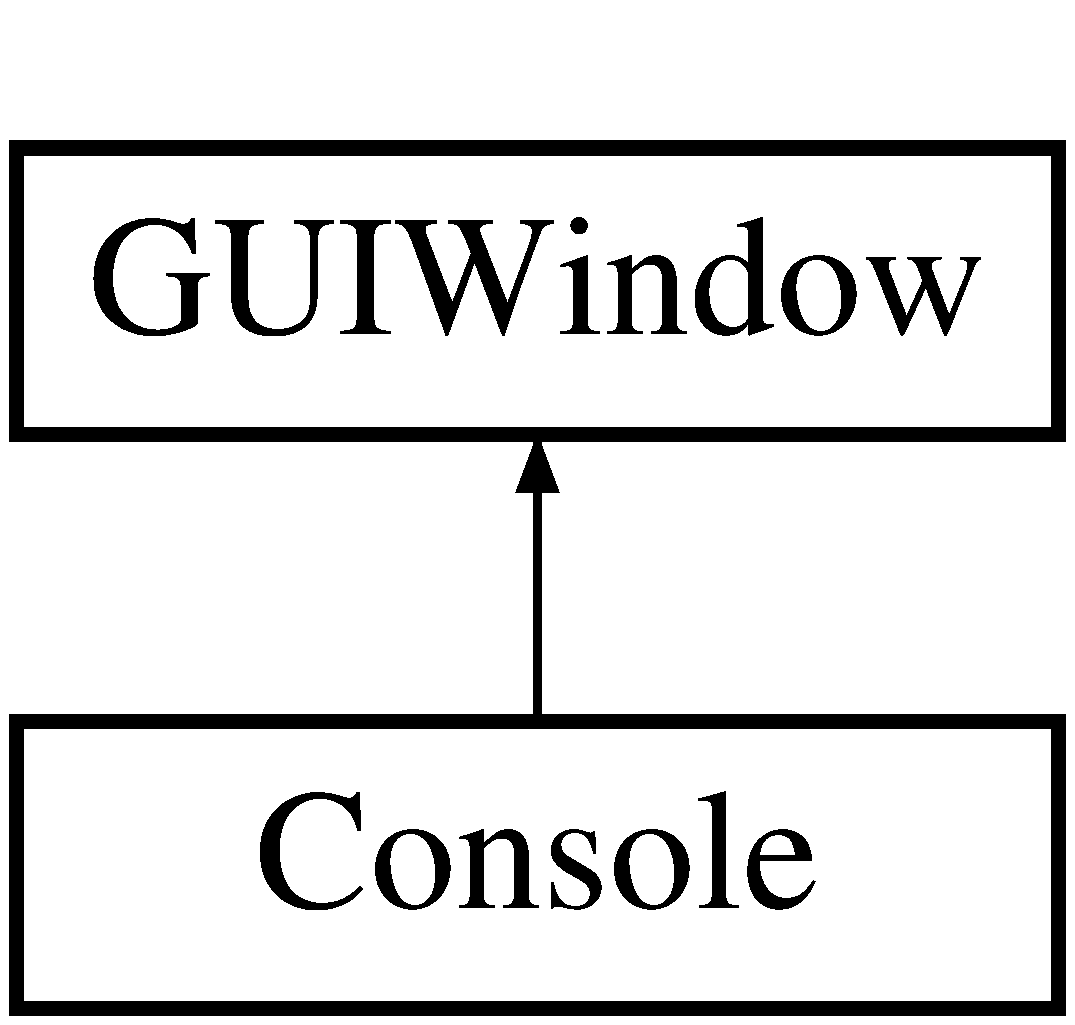
\includegraphics[height=2.000000cm]{class_console}
\end{center}
\end{figure}
\subsection*{Public Member Functions}
\begin{DoxyCompactItemize}
\item 
\hyperlink{class_console_aba16cfd9f0894eb1312b1bc1155b6646}{Console} ()
\begin{DoxyCompactList}\small\item\em Constructor. \end{DoxyCompactList}\item 
\hyperlink{class_console_a2b86176c87730295868220533308c8ab}{$\sim$\+Console} ()=default
\begin{DoxyCompactList}\small\item\em Destructor. \end{DoxyCompactList}\item 
void \hyperlink{class_console_a501dafcea40b76808dec9fce5817f54a}{set\+\_\+visible} (bool) override
\begin{DoxyCompactList}\small\item\em Changes the visibility and text capturing of the console window. \end{DoxyCompactList}\item 
bool \hyperlink{class_console_aa63491208fe0a61c7c9f6f289f0c2ed3}{handle\+\_\+text} (const C\+E\+G\+U\+I\+::\+Event\+Args \&)
\begin{DoxyCompactList}\small\item\em Event handler that is called by C\+E\+G\+UI whenever a text is entered. \end{DoxyCompactList}\item 
bool \hyperlink{class_console_a619330d0fb8ad4d4f3e38dccab9d2e7a}{execute} (const C\+E\+G\+U\+I\+::\+Event\+Args \&)
\begin{DoxyCompactList}\small\item\em Event handler that is called by C\+E\+G\+UI whenever the E\+X\+E\+C\+U\+TE button is pressed. \end{DoxyCompactList}\item 
void \hyperlink{class_console_a59cea40f9d5fb4acc894cb3a474ca003}{print\+\_\+text} (const std\+::string \&, C\+E\+G\+U\+I\+::\+Colour=C\+E\+G\+U\+I\+::\+Colour\{0x\+F\+F\+F\+F\+F\+F\+F\+F\})
\begin{DoxyCompactList}\small\item\em Prints a given message into the console window. \end{DoxyCompactList}\item 
void \hyperlink{class_console_a4df392abfe169e86b14826886105b3d0}{scroll\+\_\+down} (tdt\+::uint=1)
\begin{DoxyCompactList}\small\item\em Scrolls the console output down one line, used so that messages from the outside can scroll all the way down to the last line of the output. \end{DoxyCompactList}\item 
void \hyperlink{class_console_ac3fa9f9078ac81af758ad0bec7a10bf8}{update\+\_\+fps} (tdt\+::real, tdt\+::real)
\begin{DoxyCompactList}\small\item\em Updates the F\+PS value next to the console name. \end{DoxyCompactList}\item 
void \hyperlink{class_console_a4af831013fd544d43a8c000663fbac8d}{set\+\_\+history} (tdt\+::uint)
\begin{DoxyCompactList}\small\item\em Sets the number of entries that will be shown in the console\textquotesingle{}s history. \end{DoxyCompactList}\item 
tdt\+::uint \hyperlink{class_console_a15c0773f490a22f1598acdf90f65372e}{get\+\_\+history} () const 
\begin{DoxyCompactList}\small\item\em Returns the number of entries that will be shown in the console\textquotesingle{}s history. \end{DoxyCompactList}\item 
void \hyperlink{class_console_a8b4ffaeabbea48e1f3aa1e535ee88ab8}{clear} ()
\begin{DoxyCompactList}\small\item\em Clears the console log. \end{DoxyCompactList}\end{DoxyCompactItemize}
\subsection*{Static Public Attributes}
\begin{DoxyCompactItemize}
\item 
static const C\+E\+G\+U\+I\+::\+Colour {\bfseries R\+E\+D\+\_\+\+T\+E\+XT} = C\+E\+G\+U\+I\+::\+Colour\{1.f, 0.f, 0.f\}\hypertarget{class_console_a1ebb9fe43b05ce219b7c1e321435aa04}{}\label{class_console_a1ebb9fe43b05ce219b7c1e321435aa04}

\item 
static const C\+E\+G\+U\+I\+::\+Colour {\bfseries G\+R\+E\+E\+N\+\_\+\+T\+E\+XT} = C\+E\+G\+U\+I\+::\+Colour\{0.f, 1.f, 0.f\}\hypertarget{class_console_a74d53b40493337aa9fa3c283ad09f725}{}\label{class_console_a74d53b40493337aa9fa3c283ad09f725}

\item 
static const C\+E\+G\+U\+I\+::\+Colour {\bfseries O\+R\+A\+N\+G\+E\+\_\+\+T\+E\+XT} = C\+E\+G\+U\+I\+::\+Colour\{1.f, .\+5f, 0.\+1f\}\hypertarget{class_console_a8ddeb8af000da673295852d9f3504099}{}\label{class_console_a8ddeb8af000da673295852d9f3504099}

\item 
static const C\+E\+G\+U\+I\+::\+Colour {\bfseries B\+L\+U\+E\+\_\+\+T\+E\+XT} = C\+E\+G\+U\+I\+::\+Colour\{0.f, 0.f, 1.f\}\hypertarget{class_console_adb65ead268c66f0b337716bd5a8ca5cd}{}\label{class_console_adb65ead268c66f0b337716bd5a8ca5cd}

\end{DoxyCompactItemize}
\subsection*{Protected Member Functions}
\begin{DoxyCompactItemize}
\item 
void \hyperlink{class_console_a55d92d149dba54c67855540d5e37c9f2}{init\+\_\+} () override
\begin{DoxyCompactList}\small\item\em Initializes the console and subscribes it to events. \end{DoxyCompactList}\end{DoxyCompactItemize}
\subsection*{Private Attributes}
\begin{DoxyCompactItemize}
\item 
C\+E\+G\+U\+I\+::\+Listbox $\ast$ \hyperlink{class_console_ac8c64e8d5a77ea61af8cf6c87f6ef1cd}{list\+\_\+box\+\_\+}
\begin{DoxyCompactList}\small\item\em Pointer to the C\+E\+G\+UI List\+Box widget that serves as console output. \end{DoxyCompactList}\item 
std\+::string \hyperlink{class_console_ae1b7c7ad9e7310a6144612824065de23}{curr\+\_\+command\+\_\+}
\begin{DoxyCompactList}\small\item\em String containing the current command, allows to append more statements to it until the E\+X\+E\+C\+U\+TE button is pressed, which allows for multi-\/line Lua code. \end{DoxyCompactList}\item 
tdt\+::real \hyperlink{class_console_a03cc9dd49492a409815f1384597f89dc}{time\+\_\+since\+\_\+last\+\_\+fps\+\_\+update\+\_\+}
\begin{DoxyCompactList}\small\item\em Monitors the time passed since the fps label was last updated, used to make sure the fps update won\textquotesingle{}t slow down the game as it involves float to string conversion. \end{DoxyCompactList}\item 
tdt\+::uint \hyperlink{class_console_af83f5294b62404b4c5190d4e9a1d3ea8}{console\+\_\+history\+\_\+}
\begin{DoxyCompactList}\small\item\em Limits the number of console entries that will be shown in it\textquotesingle{}s history. \end{DoxyCompactList}\end{DoxyCompactItemize}
\subsection*{Additional Inherited Members}


\subsection{Detailed Description}
Class representing the ingame developers console that allows for runtime execution of Lua code. 

Definition at line 12 of file Console.\+hpp.



\subsection{Constructor \& Destructor Documentation}
\index{Console@{Console}!Console@{Console}}
\index{Console@{Console}!Console@{Console}}
\subsubsection[{\texorpdfstring{Console()}{Console()}}]{\setlength{\rightskip}{0pt plus 5cm}Console\+::\+Console (
\begin{DoxyParamCaption}
{}
\end{DoxyParamCaption}
)}\hypertarget{class_console_aba16cfd9f0894eb1312b1bc1155b6646}{}\label{class_console_aba16cfd9f0894eb1312b1bc1155b6646}


Constructor. 



Definition at line 10 of file Console.\+cpp.

\index{Console@{Console}!````~Console@{$\sim$\+Console}}
\index{````~Console@{$\sim$\+Console}!Console@{Console}}
\subsubsection[{\texorpdfstring{$\sim$\+Console()=default}{~Console()=default}}]{\setlength{\rightskip}{0pt plus 5cm}Console\+::$\sim$\+Console (
\begin{DoxyParamCaption}
{}
\end{DoxyParamCaption}
)\hspace{0.3cm}{\ttfamily [default]}}\hypertarget{class_console_a2b86176c87730295868220533308c8ab}{}\label{class_console_a2b86176c87730295868220533308c8ab}


Destructor. 



\subsection{Member Function Documentation}
\index{Console@{Console}!clear@{clear}}
\index{clear@{clear}!Console@{Console}}
\subsubsection[{\texorpdfstring{clear()}{clear()}}]{\setlength{\rightskip}{0pt plus 5cm}void Console\+::clear (
\begin{DoxyParamCaption}
{}
\end{DoxyParamCaption}
)}\hypertarget{class_console_a8b4ffaeabbea48e1f3aa1e535ee88ab8}{}\label{class_console_a8b4ffaeabbea48e1f3aa1e535ee88ab8}


Clears the console log. 



Definition at line 130 of file Console.\+cpp.

\index{Console@{Console}!execute@{execute}}
\index{execute@{execute}!Console@{Console}}
\subsubsection[{\texorpdfstring{execute(const C\+E\+G\+U\+I\+::\+Event\+Args \&)}{execute(const CEGUI::EventArgs &)}}]{\setlength{\rightskip}{0pt plus 5cm}bool Console\+::execute (
\begin{DoxyParamCaption}
\item[{const C\+E\+G\+U\+I\+::\+Event\+Args \&}]{args}
\end{DoxyParamCaption}
)}\hypertarget{class_console_a619330d0fb8ad4d4f3e38dccab9d2e7a}{}\label{class_console_a619330d0fb8ad4d4f3e38dccab9d2e7a}


Event handler that is called by C\+E\+G\+UI whenever the E\+X\+E\+C\+U\+TE button is pressed. 


\begin{DoxyParams}{Parameters}
{\em Reference} & to the C\+E\+G\+UI argument. \\
\hline
\end{DoxyParams}


Definition at line 44 of file Console.\+cpp.

\index{Console@{Console}!get\+\_\+history@{get\+\_\+history}}
\index{get\+\_\+history@{get\+\_\+history}!Console@{Console}}
\subsubsection[{\texorpdfstring{get\+\_\+history() const }{get_history() const }}]{\setlength{\rightskip}{0pt plus 5cm}tdt\+::uint Console\+::get\+\_\+history (
\begin{DoxyParamCaption}
{}
\end{DoxyParamCaption}
) const}\hypertarget{class_console_a15c0773f490a22f1598acdf90f65372e}{}\label{class_console_a15c0773f490a22f1598acdf90f65372e}


Returns the number of entries that will be shown in the console\textquotesingle{}s history. 



Definition at line 125 of file Console.\+cpp.

\index{Console@{Console}!handle\+\_\+text@{handle\+\_\+text}}
\index{handle\+\_\+text@{handle\+\_\+text}!Console@{Console}}
\subsubsection[{\texorpdfstring{handle\+\_\+text(const C\+E\+G\+U\+I\+::\+Event\+Args \&)}{handle_text(const CEGUI::EventArgs &)}}]{\setlength{\rightskip}{0pt plus 5cm}bool Console\+::handle\+\_\+text (
\begin{DoxyParamCaption}
\item[{const C\+E\+G\+U\+I\+::\+Event\+Args \&}]{args}
\end{DoxyParamCaption}
)}\hypertarget{class_console_aa63491208fe0a61c7c9f6f289f0c2ed3}{}\label{class_console_aa63491208fe0a61c7c9f6f289f0c2ed3}


Event handler that is called by C\+E\+G\+UI whenever a text is entered. 


\begin{DoxyParams}{Parameters}
{\em Reference} & to the C\+E\+G\+UI argument. \\
\hline
\end{DoxyParams}


Definition at line 35 of file Console.\+cpp.

\index{Console@{Console}!init\+\_\+@{init\+\_\+}}
\index{init\+\_\+@{init\+\_\+}!Console@{Console}}
\subsubsection[{\texorpdfstring{init\+\_\+() override}{init_() override}}]{\setlength{\rightskip}{0pt plus 5cm}void Console\+::init\+\_\+ (
\begin{DoxyParamCaption}
{}
\end{DoxyParamCaption}
)\hspace{0.3cm}{\ttfamily [override]}, {\ttfamily [protected]}, {\ttfamily [virtual]}}\hypertarget{class_console_a55d92d149dba54c67855540d5e37c9f2}{}\label{class_console_a55d92d149dba54c67855540d5e37c9f2}


Initializes the console and subscribes it to events. 



Implements \hyperlink{class_g_u_i_window_a2a7c011363f401a57a26cc7c7652bdfd}{G\+U\+I\+Window}.



Definition at line 15 of file Console.\+cpp.

\index{Console@{Console}!print\+\_\+text@{print\+\_\+text}}
\index{print\+\_\+text@{print\+\_\+text}!Console@{Console}}
\subsubsection[{\texorpdfstring{print\+\_\+text(const std\+::string \&, C\+E\+G\+U\+I\+::\+Colour=\+C\+E\+G\+U\+I\+::\+Colour\lcurly{}0x\+F\+F\+F\+F\+F\+F\+FF\rcurly{})}{print_text(const std::string &, CEGUI::Colour=CEGUI::Colour\{0xFFFFFFFF\})}}]{\setlength{\rightskip}{0pt plus 5cm}void Console\+::print\+\_\+text (
\begin{DoxyParamCaption}
\item[{const std\+::string \&}]{msg, }
\item[{C\+E\+G\+U\+I\+::\+Colour}]{col = {\ttfamily CEGUI\+:\+:Colour\{0xFFFFFFFF\}}}
\end{DoxyParamCaption}
)}\hypertarget{class_console_a59cea40f9d5fb4acc894cb3a474ca003}{}\label{class_console_a59cea40f9d5fb4acc894cb3a474ca003}


Prints a given message into the console window. 


\begin{DoxyParams}{Parameters}
{\em Message} & to be printed. \\
\hline
{\em Colour} & of the message text, defaults to white. \\
\hline
\end{DoxyParams}


Definition at line 82 of file Console.\+cpp.

\index{Console@{Console}!scroll\+\_\+down@{scroll\+\_\+down}}
\index{scroll\+\_\+down@{scroll\+\_\+down}!Console@{Console}}
\subsubsection[{\texorpdfstring{scroll\+\_\+down(tdt\+::uint=1)}{scroll_down(tdt::uint=1)}}]{\setlength{\rightskip}{0pt plus 5cm}void Console\+::scroll\+\_\+down (
\begin{DoxyParamCaption}
\item[{tdt\+::uint}]{num\+\_\+of\+\_\+scrolls = {\ttfamily 1}}
\end{DoxyParamCaption}
)}\hypertarget{class_console_a4df392abfe169e86b14826886105b3d0}{}\label{class_console_a4df392abfe169e86b14826886105b3d0}


Scrolls the console output down one line, used so that messages from the outside can scroll all the way down to the last line of the output. 


\begin{DoxyParams}{Parameters}
{\em Amount} & of lines to scroll. \\
\hline
\end{DoxyParams}


Definition at line 104 of file Console.\+cpp.

\index{Console@{Console}!set\+\_\+history@{set\+\_\+history}}
\index{set\+\_\+history@{set\+\_\+history}!Console@{Console}}
\subsubsection[{\texorpdfstring{set\+\_\+history(tdt\+::uint)}{set_history(tdt::uint)}}]{\setlength{\rightskip}{0pt plus 5cm}void Console\+::set\+\_\+history (
\begin{DoxyParamCaption}
\item[{tdt\+::uint}]{val}
\end{DoxyParamCaption}
)}\hypertarget{class_console_a4af831013fd544d43a8c000663fbac8d}{}\label{class_console_a4af831013fd544d43a8c000663fbac8d}


Sets the number of entries that will be shown in the console\textquotesingle{}s history. 


\begin{DoxyParams}{Parameters}
{\em The} & new entry count. \\
\hline
\end{DoxyParams}


Definition at line 120 of file Console.\+cpp.

\index{Console@{Console}!set\+\_\+visible@{set\+\_\+visible}}
\index{set\+\_\+visible@{set\+\_\+visible}!Console@{Console}}
\subsubsection[{\texorpdfstring{set\+\_\+visible(bool) override}{set_visible(bool) override}}]{\setlength{\rightskip}{0pt plus 5cm}void Console\+::set\+\_\+visible (
\begin{DoxyParamCaption}
\item[{bool}]{visible}
\end{DoxyParamCaption}
)\hspace{0.3cm}{\ttfamily [override]}, {\ttfamily [virtual]}}\hypertarget{class_console_a501dafcea40b76808dec9fce5817f54a}{}\label{class_console_a501dafcea40b76808dec9fce5817f54a}


Changes the visibility and text capturing of the console window. 


\begin{DoxyParams}{Parameters}
{\em The} & new visibility state. \\
\hline
\end{DoxyParams}


Reimplemented from \hyperlink{class_g_u_i_window_afaa290bb3bb0020e676bb546d942e528}{G\+U\+I\+Window}.



Definition at line 28 of file Console.\+cpp.

\index{Console@{Console}!update\+\_\+fps@{update\+\_\+fps}}
\index{update\+\_\+fps@{update\+\_\+fps}!Console@{Console}}
\subsubsection[{\texorpdfstring{update\+\_\+fps(tdt\+::real, tdt\+::real)}{update_fps(tdt::real, tdt::real)}}]{\setlength{\rightskip}{0pt plus 5cm}void Console\+::update\+\_\+fps (
\begin{DoxyParamCaption}
\item[{tdt\+::real}]{delta, }
\item[{tdt\+::real}]{fps}
\end{DoxyParamCaption}
)}\hypertarget{class_console_ac3fa9f9078ac81af758ad0bec7a10bf8}{}\label{class_console_ac3fa9f9078ac81af758ad0bec7a10bf8}


Updates the F\+PS value next to the console name. 


\begin{DoxyParams}{Parameters}
{\em Time} & since the last frame. \\
\hline
{\em The} & new framerate. \\
\hline
\end{DoxyParams}


Definition at line 110 of file Console.\+cpp.



\subsection{Member Data Documentation}
\index{Console@{Console}!console\+\_\+history\+\_\+@{console\+\_\+history\+\_\+}}
\index{console\+\_\+history\+\_\+@{console\+\_\+history\+\_\+}!Console@{Console}}
\subsubsection[{\texorpdfstring{console\+\_\+history\+\_\+}{console_history_}}]{\setlength{\rightskip}{0pt plus 5cm}tdt\+::uint Console\+::console\+\_\+history\+\_\+\hspace{0.3cm}{\ttfamily [private]}}\hypertarget{class_console_af83f5294b62404b4c5190d4e9a1d3ea8}{}\label{class_console_af83f5294b62404b4c5190d4e9a1d3ea8}


Limits the number of console entries that will be shown in it\textquotesingle{}s history. 



Definition at line 110 of file Console.\+hpp.

\index{Console@{Console}!curr\+\_\+command\+\_\+@{curr\+\_\+command\+\_\+}}
\index{curr\+\_\+command\+\_\+@{curr\+\_\+command\+\_\+}!Console@{Console}}
\subsubsection[{\texorpdfstring{curr\+\_\+command\+\_\+}{curr_command_}}]{\setlength{\rightskip}{0pt plus 5cm}std\+::string Console\+::curr\+\_\+command\+\_\+\hspace{0.3cm}{\ttfamily [private]}}\hypertarget{class_console_ae1b7c7ad9e7310a6144612824065de23}{}\label{class_console_ae1b7c7ad9e7310a6144612824065de23}


String containing the current command, allows to append more statements to it until the E\+X\+E\+C\+U\+TE button is pressed, which allows for multi-\/line Lua code. 



Definition at line 98 of file Console.\+hpp.

\index{Console@{Console}!list\+\_\+box\+\_\+@{list\+\_\+box\+\_\+}}
\index{list\+\_\+box\+\_\+@{list\+\_\+box\+\_\+}!Console@{Console}}
\subsubsection[{\texorpdfstring{list\+\_\+box\+\_\+}{list_box_}}]{\setlength{\rightskip}{0pt plus 5cm}C\+E\+G\+U\+I\+::\+Listbox$\ast$ Console\+::list\+\_\+box\+\_\+\hspace{0.3cm}{\ttfamily [private]}}\hypertarget{class_console_ac8c64e8d5a77ea61af8cf6c87f6ef1cd}{}\label{class_console_ac8c64e8d5a77ea61af8cf6c87f6ef1cd}


Pointer to the C\+E\+G\+UI List\+Box widget that serves as console output. 



Definition at line 91 of file Console.\+hpp.

\index{Console@{Console}!time\+\_\+since\+\_\+last\+\_\+fps\+\_\+update\+\_\+@{time\+\_\+since\+\_\+last\+\_\+fps\+\_\+update\+\_\+}}
\index{time\+\_\+since\+\_\+last\+\_\+fps\+\_\+update\+\_\+@{time\+\_\+since\+\_\+last\+\_\+fps\+\_\+update\+\_\+}!Console@{Console}}
\subsubsection[{\texorpdfstring{time\+\_\+since\+\_\+last\+\_\+fps\+\_\+update\+\_\+}{time_since_last_fps_update_}}]{\setlength{\rightskip}{0pt plus 5cm}tdt\+::real Console\+::time\+\_\+since\+\_\+last\+\_\+fps\+\_\+update\+\_\+\hspace{0.3cm}{\ttfamily [private]}}\hypertarget{class_console_a03cc9dd49492a409815f1384597f89dc}{}\label{class_console_a03cc9dd49492a409815f1384597f89dc}


Monitors the time passed since the fps label was last updated, used to make sure the fps update won\textquotesingle{}t slow down the game as it involves float to string conversion. 



Definition at line 105 of file Console.\+hpp.



The documentation for this class was generated from the following files\+:\begin{DoxyCompactItemize}
\item 
gui/Console.\+hpp\item 
gui/Console.\+cpp\end{DoxyCompactItemize}

\hypertarget{struct_constructor_component}{}\section{Constructor\+Component Struct Reference}
\label{struct_constructor_component}\index{Constructor\+Component@{Constructor\+Component}}


Contains the blueprint that gets called when an entity that has this component is created.  




{\ttfamily \#include $<$Components.\+hpp$>$}

\subsection*{Public Member Functions}
\begin{DoxyCompactItemize}
\item 
{\bfseries Constructor\+Component} (std\+::string \&\&b=\char`\"{}E\+R\+R\+OR\char`\"{})\hypertarget{struct_constructor_component_ab291d85807523b0a1b80187e39d4b7a6}{}\label{struct_constructor_component_ab291d85807523b0a1b80187e39d4b7a6}

\item 
{\bfseries Constructor\+Component} (const \hyperlink{struct_constructor_component}{Constructor\+Component} \&)=default\hypertarget{struct_constructor_component_a1bfd4f79ccf7f3237060829d2388d854}{}\label{struct_constructor_component_a1bfd4f79ccf7f3237060829d2388d854}

\item 
{\bfseries Constructor\+Component} (\hyperlink{struct_constructor_component}{Constructor\+Component} \&\&)=default\hypertarget{struct_constructor_component_a5c30a6dcdfa20d20d942291a01db5aa8}{}\label{struct_constructor_component_a5c30a6dcdfa20d20d942291a01db5aa8}

\item 
\hyperlink{struct_constructor_component}{Constructor\+Component} \& {\bfseries operator=} (const \hyperlink{struct_constructor_component}{Constructor\+Component} \&)=default\hypertarget{struct_constructor_component_aabdc97a09d8df58ef5cc340490aa6df7}{}\label{struct_constructor_component_aabdc97a09d8df58ef5cc340490aa6df7}

\item 
\hyperlink{struct_constructor_component}{Constructor\+Component} \& {\bfseries operator=} (\hyperlink{struct_constructor_component}{Constructor\+Component} \&\&)=default\hypertarget{struct_constructor_component_a1a1dfcde5f8261d2bcf682e78402e194}{}\label{struct_constructor_component_a1a1dfcde5f8261d2bcf682e78402e194}

\end{DoxyCompactItemize}
\subsection*{Public Attributes}
\begin{DoxyCompactItemize}
\item 
std\+::string {\bfseries blueprint}\hypertarget{struct_constructor_component_ac10137b6a5638c4d559ac86bf3207913}{}\label{struct_constructor_component_ac10137b6a5638c4d559ac86bf3207913}

\end{DoxyCompactItemize}
\subsection*{Static Public Attributes}
\begin{DoxyCompactItemize}
\item 
static constexpr int {\bfseries type} = 28\hypertarget{struct_constructor_component_af2c0bb91fbb21625a0eb5c24f2d4589a}{}\label{struct_constructor_component_af2c0bb91fbb21625a0eb5c24f2d4589a}

\end{DoxyCompactItemize}


\subsection{Detailed Description}
Contains the blueprint that gets called when an entity that has this component is created. 

Definition at line 669 of file Components.\+hpp.



The documentation for this struct was generated from the following file\+:\begin{DoxyCompactItemize}
\item 
Components.\+hpp\end{DoxyCompactItemize}

\hypertarget{struct_counter_component}{}\section{Counter\+Component Struct Reference}
\label{struct_counter_component}\index{Counter\+Component@{Counter\+Component}}


A simple incrementing counter.  




{\ttfamily \#include $<$Components.\+hpp$>$}

\subsection*{Public Member Functions}
\begin{DoxyCompactItemize}
\item 
{\bfseries Counter\+Component} (tdt\+::uint max=0)\hypertarget{struct_counter_component_aba4dbdeb9a4d385cb4d128d1f49e94f3}{}\label{struct_counter_component_aba4dbdeb9a4d385cb4d128d1f49e94f3}

\item 
{\bfseries Counter\+Component} (const \hyperlink{struct_counter_component}{Counter\+Component} \&)=default\hypertarget{struct_counter_component_aef348e30a859b0da76737f5d0178a259}{}\label{struct_counter_component_aef348e30a859b0da76737f5d0178a259}

\item 
{\bfseries Counter\+Component} (\hyperlink{struct_counter_component}{Counter\+Component} \&\&)=default\hypertarget{struct_counter_component_afe2269b16b576f2fa05fc25db651de54}{}\label{struct_counter_component_afe2269b16b576f2fa05fc25db651de54}

\item 
\hyperlink{struct_counter_component}{Counter\+Component} \& {\bfseries operator=} (const \hyperlink{struct_counter_component}{Counter\+Component} \&)=default\hypertarget{struct_counter_component_ac812eba966d72dfd7b8a8fd0324bb241}{}\label{struct_counter_component_ac812eba966d72dfd7b8a8fd0324bb241}

\item 
\hyperlink{struct_counter_component}{Counter\+Component} \& {\bfseries operator=} (\hyperlink{struct_counter_component}{Counter\+Component} \&\&)=default\hypertarget{struct_counter_component_a26e3a1029a1ea3c901c5a07b5209fc7a}{}\label{struct_counter_component_a26e3a1029a1ea3c901c5a07b5209fc7a}

\end{DoxyCompactItemize}
\subsection*{Public Attributes}
\begin{DoxyCompactItemize}
\item 
tdt\+::uint {\bfseries curr\+\_\+value}\hypertarget{struct_counter_component_a7fbe0d431478bd7cd3057df6a157e78f}{}\label{struct_counter_component_a7fbe0d431478bd7cd3057df6a157e78f}

\item 
tdt\+::uint {\bfseries max\+\_\+value}\hypertarget{struct_counter_component_a1203c92025bb02cd46d442d8d6bafd63}{}\label{struct_counter_component_a1203c92025bb02cd46d442d8d6bafd63}

\end{DoxyCompactItemize}
\subsection*{Static Public Attributes}
\begin{DoxyCompactItemize}
\item 
static constexpr int {\bfseries type} = 38\hypertarget{struct_counter_component_a21cdfada7885913d432ae7a66320e56f}{}\label{struct_counter_component_a21cdfada7885913d432ae7a66320e56f}

\end{DoxyCompactItemize}


\subsection{Detailed Description}
A simple incrementing counter. 

\begin{DoxyNote}{Note}
The max value is not enforced and serves only for manual checking. 
\end{DoxyNote}


Definition at line 878 of file Components.\+hpp.



The documentation for this struct was generated from the following file\+:\begin{DoxyCompactItemize}
\item 
Components.\+hpp\end{DoxyCompactItemize}

\hypertarget{structutil_1_1effect_1_1_d_a_m_a_g_e___e_f_f_e_c_t}{}\section{util\+:\+:effect\+:\+:D\+A\+M\+A\+G\+E\+\_\+\+E\+F\+F\+E\+CT Struct Reference}
\label{structutil_1_1effect_1_1_d_a_m_a_g_e___e_f_f_e_c_t}\index{util\+::effect\+::\+D\+A\+M\+A\+G\+E\+\_\+\+E\+F\+F\+E\+CT@{util\+::effect\+::\+D\+A\+M\+A\+G\+E\+\_\+\+E\+F\+F\+E\+CT}}


Deals a random damage in a given range to the entity it\textquotesingle{}s called on.  




{\ttfamily \#include $<$Effects.\+hpp$>$}

\subsection*{Public Member Functions}
\begin{DoxyCompactItemize}
\item 
\hyperlink{structutil_1_1effect_1_1_d_a_m_a_g_e___e_f_f_e_c_t_a364947d50bd41ce12e61677daa1e665d}{D\+A\+M\+A\+G\+E\+\_\+\+E\+F\+F\+E\+CT} (\hyperlink{class_entity_system}{Entity\+System} \&, tdt\+::uint, tdt\+::uint)
\begin{DoxyCompactList}\small\item\em Constructor. \end{DoxyCompactList}\item 
\hyperlink{structutil_1_1effect_1_1_d_a_m_a_g_e___e_f_f_e_c_t_a04a8dacd8ed6af8214f1c2267c68f390}{$\sim$\+D\+A\+M\+A\+G\+E\+\_\+\+E\+F\+F\+E\+CT} ()=default
\begin{DoxyCompactList}\small\item\em Destructor. \end{DoxyCompactList}\item 
void \hyperlink{structutil_1_1effect_1_1_d_a_m_a_g_e___e_f_f_e_c_t_ad561eadd4860a08de7d417798f817e68}{operator()} (tdt\+::uint)
\begin{DoxyCompactList}\small\item\em Applies the damage effect to a given entity. \end{DoxyCompactList}\end{DoxyCompactItemize}
\subsection*{Private Attributes}
\begin{DoxyCompactItemize}
\item 
tdt\+::uint \hyperlink{structutil_1_1effect_1_1_d_a_m_a_g_e___e_f_f_e_c_t_a294eef54f03197f6f26ea538daa84310}{min\+\_\+}
\begin{DoxyCompactList}\small\item\em The damage range. \end{DoxyCompactList}\item 
tdt\+::uint {\bfseries max\+\_\+}\hypertarget{structutil_1_1effect_1_1_d_a_m_a_g_e___e_f_f_e_c_t_af092bc692b6b81858e1ab984bf012f06}{}\label{structutil_1_1effect_1_1_d_a_m_a_g_e___e_f_f_e_c_t_af092bc692b6b81858e1ab984bf012f06}

\item 
\hyperlink{class_entity_system}{Entity\+System} \& \hyperlink{structutil_1_1effect_1_1_d_a_m_a_g_e___e_f_f_e_c_t_a4d2debfb657c6ee88950e249fe947087}{entities\+\_\+}
\begin{DoxyCompactList}\small\item\em Entity system containing the entities this effect will be used on. \end{DoxyCompactList}\end{DoxyCompactItemize}


\subsection{Detailed Description}
Deals a random damage in a given range to the entity it\textquotesingle{}s called on. 

Definition at line 23 of file Effects.\+hpp.



\subsection{Constructor \& Destructor Documentation}
\index{util\+::effect\+::\+D\+A\+M\+A\+G\+E\+\_\+\+E\+F\+F\+E\+CT@{util\+::effect\+::\+D\+A\+M\+A\+G\+E\+\_\+\+E\+F\+F\+E\+CT}!D\+A\+M\+A\+G\+E\+\_\+\+E\+F\+F\+E\+CT@{D\+A\+M\+A\+G\+E\+\_\+\+E\+F\+F\+E\+CT}}
\index{D\+A\+M\+A\+G\+E\+\_\+\+E\+F\+F\+E\+CT@{D\+A\+M\+A\+G\+E\+\_\+\+E\+F\+F\+E\+CT}!util\+::effect\+::\+D\+A\+M\+A\+G\+E\+\_\+\+E\+F\+F\+E\+CT@{util\+::effect\+::\+D\+A\+M\+A\+G\+E\+\_\+\+E\+F\+F\+E\+CT}}
\subsubsection[{\texorpdfstring{D\+A\+M\+A\+G\+E\+\_\+\+E\+F\+F\+E\+C\+T(\+Entity\+System \&, tdt\+::uint, tdt\+::uint)}{DAMAGE_EFFECT(EntitySystem &, tdt::uint, tdt::uint)}}]{\setlength{\rightskip}{0pt plus 5cm}util\+::effect\+::\+D\+A\+M\+A\+G\+E\+\_\+\+E\+F\+F\+E\+C\+T\+::\+D\+A\+M\+A\+G\+E\+\_\+\+E\+F\+F\+E\+CT (
\begin{DoxyParamCaption}
\item[{{\bf Entity\+System} \&}]{ents, }
\item[{tdt\+::uint}]{min, }
\item[{tdt\+::uint}]{max}
\end{DoxyParamCaption}
)}\hypertarget{structutil_1_1effect_1_1_d_a_m_a_g_e___e_f_f_e_c_t_a364947d50bd41ce12e61677daa1e665d}{}\label{structutil_1_1effect_1_1_d_a_m_a_g_e___e_f_f_e_c_t_a364947d50bd41ce12e61677daa1e665d}


Constructor. 


\begin{DoxyParams}{Parameters}
{\em Entity} & system containing the entities this effect will be used on. \\
\hline
{\em Lower} & bound of the damage range. \\
\hline
{\em Upper} & bound of the damage range. \\
\hline
\end{DoxyParams}


Definition at line 7 of file Effects.\+cpp.

\index{util\+::effect\+::\+D\+A\+M\+A\+G\+E\+\_\+\+E\+F\+F\+E\+CT@{util\+::effect\+::\+D\+A\+M\+A\+G\+E\+\_\+\+E\+F\+F\+E\+CT}!````~D\+A\+M\+A\+G\+E\+\_\+\+E\+F\+F\+E\+CT@{$\sim$\+D\+A\+M\+A\+G\+E\+\_\+\+E\+F\+F\+E\+CT}}
\index{````~D\+A\+M\+A\+G\+E\+\_\+\+E\+F\+F\+E\+CT@{$\sim$\+D\+A\+M\+A\+G\+E\+\_\+\+E\+F\+F\+E\+CT}!util\+::effect\+::\+D\+A\+M\+A\+G\+E\+\_\+\+E\+F\+F\+E\+CT@{util\+::effect\+::\+D\+A\+M\+A\+G\+E\+\_\+\+E\+F\+F\+E\+CT}}
\subsubsection[{\texorpdfstring{$\sim$\+D\+A\+M\+A\+G\+E\+\_\+\+E\+F\+F\+E\+C\+T()=default}{~DAMAGE_EFFECT()=default}}]{\setlength{\rightskip}{0pt plus 5cm}util\+::effect\+::\+D\+A\+M\+A\+G\+E\+\_\+\+E\+F\+F\+E\+C\+T\+::$\sim$\+D\+A\+M\+A\+G\+E\+\_\+\+E\+F\+F\+E\+CT (
\begin{DoxyParamCaption}
{}
\end{DoxyParamCaption}
)\hspace{0.3cm}{\ttfamily [default]}}\hypertarget{structutil_1_1effect_1_1_d_a_m_a_g_e___e_f_f_e_c_t_a04a8dacd8ed6af8214f1c2267c68f390}{}\label{structutil_1_1effect_1_1_d_a_m_a_g_e___e_f_f_e_c_t_a04a8dacd8ed6af8214f1c2267c68f390}


Destructor. 



\subsection{Member Function Documentation}
\index{util\+::effect\+::\+D\+A\+M\+A\+G\+E\+\_\+\+E\+F\+F\+E\+CT@{util\+::effect\+::\+D\+A\+M\+A\+G\+E\+\_\+\+E\+F\+F\+E\+CT}!operator()@{operator()}}
\index{operator()@{operator()}!util\+::effect\+::\+D\+A\+M\+A\+G\+E\+\_\+\+E\+F\+F\+E\+CT@{util\+::effect\+::\+D\+A\+M\+A\+G\+E\+\_\+\+E\+F\+F\+E\+CT}}
\subsubsection[{\texorpdfstring{operator()(tdt\+::uint)}{operator()(tdt::uint)}}]{\setlength{\rightskip}{0pt plus 5cm}void util\+::effect\+::\+D\+A\+M\+A\+G\+E\+\_\+\+E\+F\+F\+E\+C\+T\+::operator() (
\begin{DoxyParamCaption}
\item[{tdt\+::uint}]{id}
\end{DoxyParamCaption}
)}\hypertarget{structutil_1_1effect_1_1_d_a_m_a_g_e___e_f_f_e_c_t_ad561eadd4860a08de7d417798f817e68}{}\label{structutil_1_1effect_1_1_d_a_m_a_g_e___e_f_f_e_c_t_ad561eadd4860a08de7d417798f817e68}


Applies the damage effect to a given entity. 


\begin{DoxyParams}{Parameters}
{\em ID} & of the entity. \\
\hline
\end{DoxyParams}


Definition at line 11 of file Effects.\+cpp.



\subsection{Member Data Documentation}
\index{util\+::effect\+::\+D\+A\+M\+A\+G\+E\+\_\+\+E\+F\+F\+E\+CT@{util\+::effect\+::\+D\+A\+M\+A\+G\+E\+\_\+\+E\+F\+F\+E\+CT}!entities\+\_\+@{entities\+\_\+}}
\index{entities\+\_\+@{entities\+\_\+}!util\+::effect\+::\+D\+A\+M\+A\+G\+E\+\_\+\+E\+F\+F\+E\+CT@{util\+::effect\+::\+D\+A\+M\+A\+G\+E\+\_\+\+E\+F\+F\+E\+CT}}
\subsubsection[{\texorpdfstring{entities\+\_\+}{entities_}}]{\setlength{\rightskip}{0pt plus 5cm}{\bf Entity\+System}\& util\+::effect\+::\+D\+A\+M\+A\+G\+E\+\_\+\+E\+F\+F\+E\+C\+T\+::entities\+\_\+\hspace{0.3cm}{\ttfamily [private]}}\hypertarget{structutil_1_1effect_1_1_d_a_m_a_g_e___e_f_f_e_c_t_a4d2debfb657c6ee88950e249fe947087}{}\label{structutil_1_1effect_1_1_d_a_m_a_g_e___e_f_f_e_c_t_a4d2debfb657c6ee88950e249fe947087}


Entity system containing the entities this effect will be used on. 



Definition at line 55 of file Effects.\+hpp.

\index{util\+::effect\+::\+D\+A\+M\+A\+G\+E\+\_\+\+E\+F\+F\+E\+CT@{util\+::effect\+::\+D\+A\+M\+A\+G\+E\+\_\+\+E\+F\+F\+E\+CT}!min\+\_\+@{min\+\_\+}}
\index{min\+\_\+@{min\+\_\+}!util\+::effect\+::\+D\+A\+M\+A\+G\+E\+\_\+\+E\+F\+F\+E\+CT@{util\+::effect\+::\+D\+A\+M\+A\+G\+E\+\_\+\+E\+F\+F\+E\+CT}}
\subsubsection[{\texorpdfstring{min\+\_\+}{min_}}]{\setlength{\rightskip}{0pt plus 5cm}tdt\+::uint util\+::effect\+::\+D\+A\+M\+A\+G\+E\+\_\+\+E\+F\+F\+E\+C\+T\+::min\+\_\+\hspace{0.3cm}{\ttfamily [private]}}\hypertarget{structutil_1_1effect_1_1_d_a_m_a_g_e___e_f_f_e_c_t_a294eef54f03197f6f26ea538daa84310}{}\label{structutil_1_1effect_1_1_d_a_m_a_g_e___e_f_f_e_c_t_a294eef54f03197f6f26ea538daa84310}


The damage range. 



Definition at line 49 of file Effects.\+hpp.



The documentation for this struct was generated from the following files\+:\begin{DoxyCompactItemize}
\item 
tools/Effects.\+hpp\item 
tools/Effects.\+cpp\end{DoxyCompactItemize}

\hypertarget{struct_destructor_component}{}\section{Destructor\+Component Struct Reference}
\label{struct_destructor_component}\index{Destructor\+Component@{Destructor\+Component}}


Contains name of the table that contains the function (called \char`\"{}dtor\char`\"{}) which is called when an entity is destroyed.  




{\ttfamily \#include $<$Components.\+hpp$>$}

\subsection*{Public Member Functions}
\begin{DoxyCompactItemize}
\item 
{\bfseries Destructor\+Component} (std\+::string b=\char`\"{}E\+R\+R\+OR\char`\"{})\hypertarget{struct_destructor_component_aebc03621eaa6822682f712e58bdbd673}{}\label{struct_destructor_component_aebc03621eaa6822682f712e58bdbd673}

\item 
{\bfseries Destructor\+Component} (const \hyperlink{struct_destructor_component}{Destructor\+Component} \&)=default\hypertarget{struct_destructor_component_acfe9290b3966e8b99ccd174ee5d832ba}{}\label{struct_destructor_component_acfe9290b3966e8b99ccd174ee5d832ba}

\item 
{\bfseries Destructor\+Component} (\hyperlink{struct_destructor_component}{Destructor\+Component} \&\&)=default\hypertarget{struct_destructor_component_a64114c34c256244d6e3b5ec61a5f933a}{}\label{struct_destructor_component_a64114c34c256244d6e3b5ec61a5f933a}

\item 
\hyperlink{struct_destructor_component}{Destructor\+Component} \& {\bfseries operator=} (const \hyperlink{struct_destructor_component}{Destructor\+Component} \&)=default\hypertarget{struct_destructor_component_ae054b00544dbe4ff739cad5024d76def}{}\label{struct_destructor_component_ae054b00544dbe4ff739cad5024d76def}

\item 
\hyperlink{struct_destructor_component}{Destructor\+Component} \& {\bfseries operator=} (\hyperlink{struct_destructor_component}{Destructor\+Component} \&\&)=default\hypertarget{struct_destructor_component_a426b010b77796f43f476f906c161bf2c}{}\label{struct_destructor_component_a426b010b77796f43f476f906c161bf2c}

\end{DoxyCompactItemize}
\subsection*{Public Attributes}
\begin{DoxyCompactItemize}
\item 
std\+::string {\bfseries blueprint}\hypertarget{struct_destructor_component_a08739ab1287c35b9c53bcc0072d4baf9}{}\label{struct_destructor_component_a08739ab1287c35b9c53bcc0072d4baf9}

\end{DoxyCompactItemize}
\subsection*{Static Public Attributes}
\begin{DoxyCompactItemize}
\item 
static constexpr int {\bfseries type} = 20\hypertarget{struct_destructor_component_a1c3196707ec5bd820a3d72bd0555c1c7}{}\label{struct_destructor_component_a1c3196707ec5bd820a3d72bd0555c1c7}

\end{DoxyCompactItemize}


\subsection{Detailed Description}
Contains name of the table that contains the function (called \char`\"{}dtor\char`\"{}) which is called when an entity is destroyed. 

Definition at line 508 of file Components.\+hpp.



The documentation for this struct was generated from the following file\+:\begin{DoxyCompactItemize}
\item 
Components.\+hpp\end{DoxyCompactItemize}

\hypertarget{class_entity_creator}{}\section{Entity\+Creator Class Reference}
\label{class_entity_creator}\index{Entity\+Creator@{Entity\+Creator}}


Class representing the debugging \hyperlink{class_g_u_i}{G\+UI} window used to place and create entities during runtime.  




{\ttfamily \#include $<$Entity\+Creator.\+hpp$>$}

Inheritance diagram for Entity\+Creator\+:\begin{figure}[H]
\begin{center}
\leavevmode
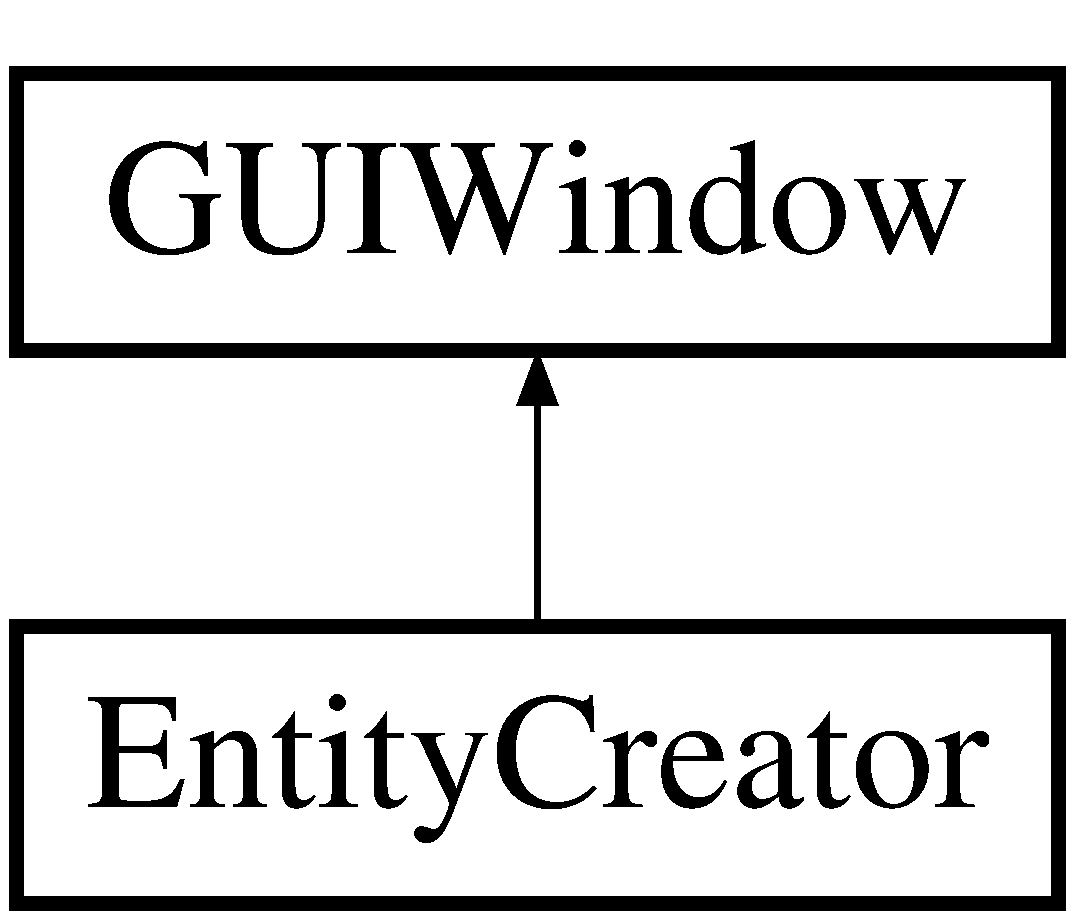
\includegraphics[height=2.000000cm]{class_entity_creator}
\end{center}
\end{figure}
\subsection*{Public Member Functions}
\begin{DoxyCompactItemize}
\item 
\hyperlink{class_entity_creator_a980c1beb6678a23e40f34a821099ca73}{Entity\+Creator} (\hyperlink{class_entity_placer}{Entity\+Placer} \&, \hyperlink{class_entity_system}{Entity\+System} \&)
\begin{DoxyCompactList}\small\item\em Constructor, loads the gui layout for this window and registers callbacks. \end{DoxyCompactList}\item 
\hyperlink{class_entity_creator_a070bdc284ddbd15dc8359b4bdf960e9c}{$\sim$\+Entity\+Creator} ()
\begin{DoxyCompactList}\small\item\em Destructor. \end{DoxyCompactList}\item 
bool \hyperlink{class_entity_creator_a7ed9e893dbbee279a85a7b4479fc5e8c}{place} (const C\+E\+G\+U\+I\+::\+Event\+Args \&)
\begin{DoxyCompactList}\small\item\em Function that is called when the player/developer presses the \char`\"{}place now\char`\"{} button, sets the currently selected entity blueprint for placing. \end{DoxyCompactList}\item 
bool \hyperlink{class_entity_creator_a7b114e5282d17e6a2ec7dc7219a14fe2}{change\+\_\+to\+\_\+place} (const C\+E\+G\+U\+I\+::\+Event\+Args \&)
\begin{DoxyCompactList}\small\item\em Function that is called when the player/developer presses the \char`\"{}place\char`\"{} button, changing the creator to the placing mode. \end{DoxyCompactList}\item 
bool \hyperlink{class_entity_creator_ae055603836c5c525dcdf7a9a850fb600}{change\+\_\+to\+\_\+create} (const C\+E\+G\+U\+I\+::\+Event\+Args \&)
\begin{DoxyCompactList}\small\item\em Function that is called when the player/developer presses the \char`\"{}create\char`\"{} button, changing the creator to the creation mode. \end{DoxyCompactList}\item 
bool \hyperlink{class_entity_creator_a3f0182b955bc10f344c5df5c293bb618}{actualize\+\_\+list} (const C\+E\+G\+U\+I\+::\+Event\+Args \&)
\begin{DoxyCompactList}\small\item\em Function that is called when the player/developer presses the \char`\"{}actualize
       list\char`\"{} button and displays the set of all selected entities to the list box. \end{DoxyCompactList}\end{DoxyCompactItemize}
\subsection*{Protected Member Functions}
\begin{DoxyCompactItemize}
\item 
void \hyperlink{class_entity_creator_a6450f0e4239b4eb3dc3c8224371c564f}{init\+\_\+} () override
\begin{DoxyCompactList}\small\item\em Initializes the \hyperlink{class_entity_creator}{Entity\+Creator}. \end{DoxyCompactList}\end{DoxyCompactItemize}
\subsection*{Private Attributes}
\begin{DoxyCompactItemize}
\item 
\hyperlink{class_entity_placer}{Entity\+Placer} \& \hyperlink{class_entity_creator_a9391bd0312fc88528dbb7533a835daaf}{placer\+\_\+}
\begin{DoxyCompactList}\small\item\em Reference to the game\textquotesingle{}s entity placer, used to set the blueprint table and visibility mode when the player/developer presses the \char`\"{}place now\char`\"{} button. \end{DoxyCompactList}\item 
std\+::set$<$ std\+::string $>$ \& \hyperlink{class_entity_creator_a15d7d05f00f1fadb0bbba6170b98c2e1}{registered\+\_\+entities\+\_\+}
\begin{DoxyCompactList}\small\item\em Reference to the list of all registered entity blueprint names used for updates. \end{DoxyCompactList}\item 
C\+E\+G\+U\+I\+::\+Listbox $\ast$ \hyperlink{class_entity_creator_a8bed2a552aa8b2292564d50be8a3baaa}{list\+\_\+box\+\_\+}
\begin{DoxyCompactList}\small\item\em Auxiliary pointer to the list box sub window for easy access when updating the entity blueprint list. \end{DoxyCompactList}\end{DoxyCompactItemize}
\subsection*{Additional Inherited Members}


\subsection{Detailed Description}
Class representing the debugging \hyperlink{class_g_u_i}{G\+UI} window used to place and create entities during runtime. 

Definition at line 14 of file Entity\+Creator.\+hpp.



\subsection{Constructor \& Destructor Documentation}
\index{Entity\+Creator@{Entity\+Creator}!Entity\+Creator@{Entity\+Creator}}
\index{Entity\+Creator@{Entity\+Creator}!Entity\+Creator@{Entity\+Creator}}
\subsubsection[{\texorpdfstring{Entity\+Creator(\+Entity\+Placer \&, Entity\+System \&)}{EntityCreator(EntityPlacer &, EntitySystem &)}}]{\setlength{\rightskip}{0pt plus 5cm}Entity\+Creator\+::\+Entity\+Creator (
\begin{DoxyParamCaption}
\item[{{\bf Entity\+Placer} \&}]{placer, }
\item[{{\bf Entity\+System} \&}]{ents}
\end{DoxyParamCaption}
)}\hypertarget{class_entity_creator_a980c1beb6678a23e40f34a821099ca73}{}\label{class_entity_creator_a980c1beb6678a23e40f34a821099ca73}


Constructor, loads the gui layout for this window and registers callbacks. 


\begin{DoxyParams}{Parameters}
{\em Reference} & to the game\textquotesingle{}s entity placer. \\
\hline
{\em Reference} & to the game\textquotesingle{}s entity system. \\
\hline
\end{DoxyParams}


Definition at line 6 of file Entity\+Creator.\+cpp.

\index{Entity\+Creator@{Entity\+Creator}!````~Entity\+Creator@{$\sim$\+Entity\+Creator}}
\index{````~Entity\+Creator@{$\sim$\+Entity\+Creator}!Entity\+Creator@{Entity\+Creator}}
\subsubsection[{\texorpdfstring{$\sim$\+Entity\+Creator()}{~EntityCreator()}}]{\setlength{\rightskip}{0pt plus 5cm}Entity\+Creator\+::$\sim$\+Entity\+Creator (
\begin{DoxyParamCaption}
{}
\end{DoxyParamCaption}
)\hspace{0.3cm}{\ttfamily [inline]}}\hypertarget{class_entity_creator_a070bdc284ddbd15dc8359b4bdf960e9c}{}\label{class_entity_creator_a070bdc284ddbd15dc8359b4bdf960e9c}


Destructor. 



Definition at line 27 of file Entity\+Creator.\+hpp.



\subsection{Member Function Documentation}
\index{Entity\+Creator@{Entity\+Creator}!actualize\+\_\+list@{actualize\+\_\+list}}
\index{actualize\+\_\+list@{actualize\+\_\+list}!Entity\+Creator@{Entity\+Creator}}
\subsubsection[{\texorpdfstring{actualize\+\_\+list(const C\+E\+G\+U\+I\+::\+Event\+Args \&)}{actualize_list(const CEGUI::EventArgs &)}}]{\setlength{\rightskip}{0pt plus 5cm}bool Entity\+Creator\+::actualize\+\_\+list (
\begin{DoxyParamCaption}
\item[{const C\+E\+G\+U\+I\+::\+Event\+Args \&}]{args}
\end{DoxyParamCaption}
)}\hypertarget{class_entity_creator_a3f0182b955bc10f344c5df5c293bb618}{}\label{class_entity_creator_a3f0182b955bc10f344c5df5c293bb618}


Function that is called when the player/developer presses the \char`\"{}actualize
       list\char`\"{} button and displays the set of all selected entities to the list box. 


\begin{DoxyParams}{Parameters}
{\em Reference} & to the C\+E\+G\+UI event arguments. \\
\hline
\end{DoxyParams}


Definition at line 34 of file Entity\+Creator.\+cpp.

\index{Entity\+Creator@{Entity\+Creator}!change\+\_\+to\+\_\+create@{change\+\_\+to\+\_\+create}}
\index{change\+\_\+to\+\_\+create@{change\+\_\+to\+\_\+create}!Entity\+Creator@{Entity\+Creator}}
\subsubsection[{\texorpdfstring{change\+\_\+to\+\_\+create(const C\+E\+G\+U\+I\+::\+Event\+Args \&)}{change_to_create(const CEGUI::EventArgs &)}}]{\setlength{\rightskip}{0pt plus 5cm}bool Entity\+Creator\+::change\+\_\+to\+\_\+create (
\begin{DoxyParamCaption}
\item[{const C\+E\+G\+U\+I\+::\+Event\+Args \&}]{args}
\end{DoxyParamCaption}
)}\hypertarget{class_entity_creator_ae055603836c5c525dcdf7a9a850fb600}{}\label{class_entity_creator_ae055603836c5c525dcdf7a9a850fb600}


Function that is called when the player/developer presses the \char`\"{}create\char`\"{} button, changing the creator to the creation mode. 


\begin{DoxyParams}{Parameters}
{\em Reference} & to the C\+E\+G\+UI event arguments. \\
\hline
\end{DoxyParams}


Definition at line 28 of file Entity\+Creator.\+cpp.

\index{Entity\+Creator@{Entity\+Creator}!change\+\_\+to\+\_\+place@{change\+\_\+to\+\_\+place}}
\index{change\+\_\+to\+\_\+place@{change\+\_\+to\+\_\+place}!Entity\+Creator@{Entity\+Creator}}
\subsubsection[{\texorpdfstring{change\+\_\+to\+\_\+place(const C\+E\+G\+U\+I\+::\+Event\+Args \&)}{change_to_place(const CEGUI::EventArgs &)}}]{\setlength{\rightskip}{0pt plus 5cm}bool Entity\+Creator\+::change\+\_\+to\+\_\+place (
\begin{DoxyParamCaption}
\item[{const C\+E\+G\+U\+I\+::\+Event\+Args \&}]{args}
\end{DoxyParamCaption}
)}\hypertarget{class_entity_creator_a7b114e5282d17e6a2ec7dc7219a14fe2}{}\label{class_entity_creator_a7b114e5282d17e6a2ec7dc7219a14fe2}


Function that is called when the player/developer presses the \char`\"{}place\char`\"{} button, changing the creator to the placing mode. 


\begin{DoxyParams}{Parameters}
{\em Reference} & to the C\+E\+G\+UI event arguments. \\
\hline
\end{DoxyParams}


Definition at line 22 of file Entity\+Creator.\+cpp.

\index{Entity\+Creator@{Entity\+Creator}!init\+\_\+@{init\+\_\+}}
\index{init\+\_\+@{init\+\_\+}!Entity\+Creator@{Entity\+Creator}}
\subsubsection[{\texorpdfstring{init\+\_\+() override}{init_() override}}]{\setlength{\rightskip}{0pt plus 5cm}void Entity\+Creator\+::init\+\_\+ (
\begin{DoxyParamCaption}
{}
\end{DoxyParamCaption}
)\hspace{0.3cm}{\ttfamily [override]}, {\ttfamily [protected]}, {\ttfamily [virtual]}}\hypertarget{class_entity_creator_a6450f0e4239b4eb3dc3c8224371c564f}{}\label{class_entity_creator_a6450f0e4239b4eb3dc3c8224371c564f}


Initializes the \hyperlink{class_entity_creator}{Entity\+Creator}. 



Implements \hyperlink{class_g_u_i_window_a2a7c011363f401a57a26cc7c7652bdfd}{G\+U\+I\+Window}.



Definition at line 51 of file Entity\+Creator.\+cpp.

\index{Entity\+Creator@{Entity\+Creator}!place@{place}}
\index{place@{place}!Entity\+Creator@{Entity\+Creator}}
\subsubsection[{\texorpdfstring{place(const C\+E\+G\+U\+I\+::\+Event\+Args \&)}{place(const CEGUI::EventArgs &)}}]{\setlength{\rightskip}{0pt plus 5cm}bool Entity\+Creator\+::place (
\begin{DoxyParamCaption}
\item[{const C\+E\+G\+U\+I\+::\+Event\+Args \&}]{args}
\end{DoxyParamCaption}
)}\hypertarget{class_entity_creator_a7ed9e893dbbee279a85a7b4479fc5e8c}{}\label{class_entity_creator_a7ed9e893dbbee279a85a7b4479fc5e8c}


Function that is called when the player/developer presses the \char`\"{}place now\char`\"{} button, sets the currently selected entity blueprint for placing. 


\begin{DoxyParams}{Parameters}
{\em Reference} & to the C\+E\+G\+UI event arguments. \\
\hline
\end{DoxyParams}


Definition at line 10 of file Entity\+Creator.\+cpp.



\subsection{Member Data Documentation}
\index{Entity\+Creator@{Entity\+Creator}!list\+\_\+box\+\_\+@{list\+\_\+box\+\_\+}}
\index{list\+\_\+box\+\_\+@{list\+\_\+box\+\_\+}!Entity\+Creator@{Entity\+Creator}}
\subsubsection[{\texorpdfstring{list\+\_\+box\+\_\+}{list_box_}}]{\setlength{\rightskip}{0pt plus 5cm}C\+E\+G\+U\+I\+::\+Listbox$\ast$ Entity\+Creator\+::list\+\_\+box\+\_\+\hspace{0.3cm}{\ttfamily [private]}}\hypertarget{class_entity_creator_a8bed2a552aa8b2292564d50be8a3baaa}{}\label{class_entity_creator_a8bed2a552aa8b2292564d50be8a3baaa}


Auxiliary pointer to the list box sub window for easy access when updating the entity blueprint list. 



Definition at line 80 of file Entity\+Creator.\+hpp.

\index{Entity\+Creator@{Entity\+Creator}!placer\+\_\+@{placer\+\_\+}}
\index{placer\+\_\+@{placer\+\_\+}!Entity\+Creator@{Entity\+Creator}}
\subsubsection[{\texorpdfstring{placer\+\_\+}{placer_}}]{\setlength{\rightskip}{0pt plus 5cm}{\bf Entity\+Placer}\& Entity\+Creator\+::placer\+\_\+\hspace{0.3cm}{\ttfamily [private]}}\hypertarget{class_entity_creator_a9391bd0312fc88528dbb7533a835daaf}{}\label{class_entity_creator_a9391bd0312fc88528dbb7533a835daaf}


Reference to the game\textquotesingle{}s entity placer, used to set the blueprint table and visibility mode when the player/developer presses the \char`\"{}place now\char`\"{} button. 



Definition at line 69 of file Entity\+Creator.\+hpp.

\index{Entity\+Creator@{Entity\+Creator}!registered\+\_\+entities\+\_\+@{registered\+\_\+entities\+\_\+}}
\index{registered\+\_\+entities\+\_\+@{registered\+\_\+entities\+\_\+}!Entity\+Creator@{Entity\+Creator}}
\subsubsection[{\texorpdfstring{registered\+\_\+entities\+\_\+}{registered_entities_}}]{\setlength{\rightskip}{0pt plus 5cm}std\+::set$<$std\+::string$>$\& Entity\+Creator\+::registered\+\_\+entities\+\_\+\hspace{0.3cm}{\ttfamily [private]}}\hypertarget{class_entity_creator_a15d7d05f00f1fadb0bbba6170b98c2e1}{}\label{class_entity_creator_a15d7d05f00f1fadb0bbba6170b98c2e1}


Reference to the list of all registered entity blueprint names used for updates. 



Definition at line 74 of file Entity\+Creator.\+hpp.



The documentation for this class was generated from the following files\+:\begin{DoxyCompactItemize}
\item 
gui/Entity\+Creator.\+hpp\item 
gui/Entity\+Creator.\+cpp\end{DoxyCompactItemize}

\hypertarget{classutil_1_1_entity_destroyer}{}\section{util\+:\+:Entity\+Destroyer Class Reference}
\label{classutil_1_1_entity_destroyer}\index{util\+::\+Entity\+Destroyer@{util\+::\+Entity\+Destroyer}}


A structure providing the private method \hyperlink{class_entity_system_a4ecd6127995602d98736cd1cf5799c11}{Entity\+System\+::destroy\+\_\+entity} to the \hyperlink{namespace_destructor_helper_a93b8f71a2769c231679141fcef275bdb}{Destructor\+Helper\+::destroy} function.  




{\ttfamily \#include $<$Util.\+hpp$>$}

\subsection*{Static Private Member Functions}
\begin{DoxyCompactItemize}
\item 
static void \hyperlink{classutil_1_1_entity_destroyer_ae6df56bd2fc643398bf1de3155d0c71a}{destroy} (\hyperlink{class_entity_system}{Entity\+System} \&, tdt\+::uint)
\begin{DoxyCompactList}\small\item\em Destroy a given entity. \end{DoxyCompactList}\end{DoxyCompactItemize}
\subsection*{Friends}
\begin{DoxyCompactItemize}
\item 
void {\bfseries Destructor\+Helper\+::destroy} (\hyperlink{class_entity_system}{Entity\+System} \&, tdt\+::uint, bool, tdt\+::uint)\hypertarget{classutil_1_1_entity_destroyer_a43c94aa2e0a779761e17a5b17ce6d83a}{}\label{classutil_1_1_entity_destroyer_a43c94aa2e0a779761e17a5b17ce6d83a}

\end{DoxyCompactItemize}


\subsection{Detailed Description}
A structure providing the private method \hyperlink{class_entity_system_a4ecd6127995602d98736cd1cf5799c11}{Entity\+System\+::destroy\+\_\+entity} to the \hyperlink{namespace_destructor_helper_a93b8f71a2769c231679141fcef275bdb}{Destructor\+Helper\+::destroy} function. 

The reason for the existence of this struct is that it provides only this one method and keeps others private. 

Definition at line 194 of file Util.\+hpp.



\subsection{Member Function Documentation}
\index{util\+::\+Entity\+Destroyer@{util\+::\+Entity\+Destroyer}!destroy@{destroy}}
\index{destroy@{destroy}!util\+::\+Entity\+Destroyer@{util\+::\+Entity\+Destroyer}}
\subsubsection[{\texorpdfstring{destroy(\+Entity\+System \&, tdt\+::uint)}{destroy(EntitySystem &, tdt::uint)}}]{\setlength{\rightskip}{0pt plus 5cm}void util\+::\+Entity\+Destroyer\+::destroy (
\begin{DoxyParamCaption}
\item[{{\bf Entity\+System} \&}]{ents, }
\item[{tdt\+::uint}]{id}
\end{DoxyParamCaption}
)\hspace{0.3cm}{\ttfamily [static]}, {\ttfamily [private]}}\hypertarget{classutil_1_1_entity_destroyer_ae6df56bd2fc643398bf1de3155d0c71a}{}\label{classutil_1_1_entity_destroyer_ae6df56bd2fc643398bf1de3155d0c71a}


Destroy a given entity. 


\begin{DoxyParams}{Parameters}
{\em Entity} & system containing the entity. \\
\hline
{\em ID} & of the entity. \\
\hline
\end{DoxyParams}


Definition at line 40 of file Util.\+cpp.



The documentation for this class was generated from the following files\+:\begin{DoxyCompactItemize}
\item 
tools/Util.\+hpp\item 
tools/Util.\+cpp\end{DoxyCompactItemize}

\hypertarget{class_entity_placer}{}\section{Entity\+Placer Class Reference}
\label{class_entity_placer}\index{Entity\+Placer@{Entity\+Placer}}


Class allowing the player/developer to place entities on the ground.  




{\ttfamily \#include $<$Entity\+Placer.\+hpp$>$}

\subsection*{Public Member Functions}
\begin{DoxyCompactItemize}
\item 
\hyperlink{class_entity_placer_ab2ee072da3a1584b8ffbe6f1d299dcc7}{Entity\+Placer} (\hyperlink{class_entity_system}{Entity\+System} \&, \hyperlink{class_grid_system}{Grid\+System} \&, Ogre\+::\+Scene\+Manager \&)
\begin{DoxyCompactList}\small\item\em Constructor. \end{DoxyCompactList}\item 
\hyperlink{class_entity_placer_aa95644c347070f209bc01dc2f2391851}{$\sim$\+Entity\+Placer} ()
\begin{DoxyCompactList}\small\item\em Destructor. \end{DoxyCompactList}\item 
void \hyperlink{class_entity_placer_af8870b8ce74e91a02f7675a3c8a2a692}{set\+\_\+current\+\_\+entity\+\_\+table} (const std\+::string \&, bool=false)
\begin{DoxyCompactList}\small\item\em Checks if a given entity blueprint contains a graphics component and if so, sets it as the currently placed entity by creating a dummy entity following the cursor. \end{DoxyCompactList}\item 
void \hyperlink{class_entity_placer_a0314d1d228bff8b317b89481aa92c361}{update\+\_\+position} (const Ogre\+::\+Vector3 \&)
\begin{DoxyCompactList}\small\item\em Called every frame when the entity placer is active, adjusts the dummy entity\textquotesingle{}s position to the cursor\textquotesingle{}s. \end{DoxyCompactList}\item 
tdt\+::uint \hyperlink{class_entity_placer_a29dd8e6e72ae7b0816be797e22392260}{place} ()
\begin{DoxyCompactList}\small\item\em Creates a new entity from the blueprint table at the mouse cursor\textquotesingle{}s current position and informs the developer in the developer console. \end{DoxyCompactList}\item 
void \hyperlink{class_entity_placer_a751003cd67901a18fae7d888394cf360}{set\+\_\+visible} (bool)
\begin{DoxyCompactList}\small\item\em Sets the visibility status of the placer (and it\textquotesingle{}s dummy entity). \end{DoxyCompactList}\item 
bool \hyperlink{class_entity_placer_aefbb8b16e6f7336b999231ebb021ba52}{is\+\_\+visible} () const 
\begin{DoxyCompactList}\small\item\em Returns true if the placer is currently active (and thus the dummy entity visible), false otherwise. \end{DoxyCompactList}\item 
void \hyperlink{class_entity_placer_ae207c65665d039caa6a16c8fcb15219a}{toggle\+\_\+placing\+\_\+when\+\_\+game\+\_\+paused} ()
\begin{DoxyCompactList}\small\item\em Toggles (=negates) the flag for entity placing while the game is paused. \end{DoxyCompactList}\item 
bool \hyperlink{class_entity_placer_afe268719c2c4e17bc30713452cead93d}{can\+\_\+place\+\_\+when\+\_\+game\+\_\+paused} () const 
\begin{DoxyCompactList}\small\item\em Returns true if the placer can place entities when the game is paused, false otherwise. \end{DoxyCompactList}\end{DoxyCompactItemize}
\subsection*{Private Attributes}
\begin{DoxyCompactItemize}
\item 
\hyperlink{class_entity_system}{Entity\+System} \& \hyperlink{class_entity_placer_ae9fd5bc815ebbfd3edaeda50c3514db6}{entities\+\_\+}
\begin{DoxyCompactList}\small\item\em Reference to the game\textquotesingle{}s entity system. \end{DoxyCompactList}\item 
\hyperlink{class_grid_system}{Grid\+System} \& \hyperlink{class_entity_placer_ab83d8094255391c2ad998dad77420510}{grid\+\_\+}
\begin{DoxyCompactList}\small\item\em Reference to the game\textquotesingle{}s grid system. \end{DoxyCompactList}\item 
Ogre\+::\+Vector3 \hyperlink{class_entity_placer_a27b04e112365310f41af57bc764fc595}{curr\+\_\+position\+\_\+}
\begin{DoxyCompactList}\small\item\em Current position of the dummy entity (used to avoid the need to pass the position again on the actual placement cal). \end{DoxyCompactList}\item 
Ogre\+::\+Scene\+Node $\ast$ \hyperlink{class_entity_placer_a6e7d6a22bb82c701ef9a1be971de9205}{placing\+\_\+node\+\_\+}
\begin{DoxyCompactList}\small\item\em Pointer to the scene node the dummy entity is attached to. \end{DoxyCompactList}\item 
bool \hyperlink{class_entity_placer_ad54b47813b660f962dcd04378ebf3ecd}{visible\+\_\+}
\begin{DoxyCompactList}\small\item\em The placer\textquotesingle{}s visibility (and active) status. \end{DoxyCompactList}\item 
std\+::string \hyperlink{class_entity_placer_a51c07b2b7a1a2e66334fd961aea2bff4}{table\+\_\+name\+\_\+}
\begin{DoxyCompactList}\small\item\em Name of the blueprint of the currently placed entity. \end{DoxyCompactList}\item 
tdt\+::real \hyperlink{class_entity_placer_a72d45d5edaff74b58a898a7ad1b518fc}{half\+\_\+height\+\_\+}
\begin{DoxyCompactList}\small\item\em Used to correctly place the newly created entity on the ground. \end{DoxyCompactList}\item 
bool \hyperlink{class_entity_placer_af3edb9c35afa51723737c9995bdd2f84}{placing\+\_\+structure\+\_\+}
\begin{DoxyCompactList}\small\item\em Determines if a structure (wall, building etc.) is being placed, this will make the dummy entity to snap to the grid nodes. \end{DoxyCompactList}\item 
tdt\+::uint \hyperlink{class_entity_placer_a329869555fb8492752f6deccf1678a98}{structure\+\_\+radius\+\_\+}
\begin{DoxyCompactList}\small\item\em Radius of the placed structure (if it\textquotesingle{}s covering more than one node). \end{DoxyCompactList}\item 
Ogre\+::\+Scene\+Manager \& \hyperlink{class_entity_placer_ad80a74a9b6ee426c6050b825d3c78aea}{mgr\+\_\+}
\begin{DoxyCompactList}\small\item\em Scene manager used to hold the dummy node and manipulate models. \end{DoxyCompactList}\item 
Ogre\+::\+Entity $\ast$ \hyperlink{class_entity_placer_ae0452120158b3f88eba7b913257f185a}{ent\+\_\+}
\begin{DoxyCompactList}\small\item\em Entity representing the mesh of the placed object. \end{DoxyCompactList}\item 
tdt\+::uint \hyperlink{class_entity_placer_a936cda73ed84004f4c7b339481c6124b}{price\+\_\+}
\begin{DoxyCompactList}\small\item\em Price of the currently placed entity. \end{DoxyCompactList}\item 
bool \hyperlink{class_entity_placer_a9c038f93f3f2d94e322b050a1eafef6e}{can\+\_\+place\+\_\+when\+\_\+game\+\_\+paused\+\_\+} \{false\}
\begin{DoxyCompactList}\small\item\em Used for debugging, allows to place spawners when the game is paused and this their production is halted. \end{DoxyCompactList}\end{DoxyCompactItemize}


\subsection{Detailed Description}
Class allowing the player/developer to place entities on the ground. 

(Mainly used by the \hyperlink{class_entity_creator}{Entity\+Creator} class, but can be invoked by \char`\"{}game.\+place\+\_\+entity(\+T\+A\+B\+L\+E)\char`\"{} where T\+A\+B\+LE is the name of the desired entity\textquotesingle{}s blueprint) 

Definition at line 15 of file Entity\+Placer.\+hpp.



\subsection{Constructor \& Destructor Documentation}
\index{Entity\+Placer@{Entity\+Placer}!Entity\+Placer@{Entity\+Placer}}
\index{Entity\+Placer@{Entity\+Placer}!Entity\+Placer@{Entity\+Placer}}
\subsubsection[{\texorpdfstring{Entity\+Placer(\+Entity\+System \&, Grid\+System \&, Ogre\+::\+Scene\+Manager \&)}{EntityPlacer(EntitySystem &, GridSystem &, Ogre::SceneManager &)}}]{\setlength{\rightskip}{0pt plus 5cm}Entity\+Placer\+::\+Entity\+Placer (
\begin{DoxyParamCaption}
\item[{{\bf Entity\+System} \&}]{ents, }
\item[{{\bf Grid\+System} \&}]{grid, }
\item[{Ogre\+::\+Scene\+Manager \&}]{mgr}
\end{DoxyParamCaption}
)}\hypertarget{class_entity_placer_ab2ee072da3a1584b8ffbe6f1d299dcc7}{}\label{class_entity_placer_ab2ee072da3a1584b8ffbe6f1d299dcc7}


Constructor. 


\begin{DoxyParams}{Parameters}
{\em Reference} & to the game\textquotesingle{}s entity system. \\
\hline
{\em Reference} & to the game\textquotesingle{}s grid system, used for node snapping when placing structures (i.\+e. walls, buildings...). \\
\hline
{\em Scene} & manager that will hold the dummy node. \\
\hline
\end{DoxyParams}


Definition at line 8 of file Entity\+Placer.\+cpp.

\index{Entity\+Placer@{Entity\+Placer}!````~Entity\+Placer@{$\sim$\+Entity\+Placer}}
\index{````~Entity\+Placer@{$\sim$\+Entity\+Placer}!Entity\+Placer@{Entity\+Placer}}
\subsubsection[{\texorpdfstring{$\sim$\+Entity\+Placer()}{~EntityPlacer()}}]{\setlength{\rightskip}{0pt plus 5cm}Entity\+Placer\+::$\sim$\+Entity\+Placer (
\begin{DoxyParamCaption}
{}
\end{DoxyParamCaption}
)}\hypertarget{class_entity_placer_aa95644c347070f209bc01dc2f2391851}{}\label{class_entity_placer_aa95644c347070f209bc01dc2f2391851}


Destructor. 



Definition at line 15 of file Entity\+Placer.\+cpp.



\subsection{Member Function Documentation}
\index{Entity\+Placer@{Entity\+Placer}!can\+\_\+place\+\_\+when\+\_\+game\+\_\+paused@{can\+\_\+place\+\_\+when\+\_\+game\+\_\+paused}}
\index{can\+\_\+place\+\_\+when\+\_\+game\+\_\+paused@{can\+\_\+place\+\_\+when\+\_\+game\+\_\+paused}!Entity\+Placer@{Entity\+Placer}}
\subsubsection[{\texorpdfstring{can\+\_\+place\+\_\+when\+\_\+game\+\_\+paused() const }{can_place_when_game_paused() const }}]{\setlength{\rightskip}{0pt plus 5cm}bool Entity\+Placer\+::can\+\_\+place\+\_\+when\+\_\+game\+\_\+paused (
\begin{DoxyParamCaption}
{}
\end{DoxyParamCaption}
) const}\hypertarget{class_entity_placer_afe268719c2c4e17bc30713452cead93d}{}\label{class_entity_placer_afe268719c2c4e17bc30713452cead93d}


Returns true if the placer can place entities when the game is paused, false otherwise. 



Definition at line 154 of file Entity\+Placer.\+cpp.

\index{Entity\+Placer@{Entity\+Placer}!is\+\_\+visible@{is\+\_\+visible}}
\index{is\+\_\+visible@{is\+\_\+visible}!Entity\+Placer@{Entity\+Placer}}
\subsubsection[{\texorpdfstring{is\+\_\+visible() const }{is_visible() const }}]{\setlength{\rightskip}{0pt plus 5cm}bool Entity\+Placer\+::is\+\_\+visible (
\begin{DoxyParamCaption}
{}
\end{DoxyParamCaption}
) const}\hypertarget{class_entity_placer_aefbb8b16e6f7336b999231ebb021ba52}{}\label{class_entity_placer_aefbb8b16e6f7336b999231ebb021ba52}


Returns true if the placer is currently active (and thus the dummy entity visible), false otherwise. 



Definition at line 144 of file Entity\+Placer.\+cpp.

\index{Entity\+Placer@{Entity\+Placer}!place@{place}}
\index{place@{place}!Entity\+Placer@{Entity\+Placer}}
\subsubsection[{\texorpdfstring{place()}{place()}}]{\setlength{\rightskip}{0pt plus 5cm}tdt\+::uint Entity\+Placer\+::place (
\begin{DoxyParamCaption}
{}
\end{DoxyParamCaption}
)}\hypertarget{class_entity_placer_a29dd8e6e72ae7b0816be797e22392260}{}\label{class_entity_placer_a29dd8e6e72ae7b0816be797e22392260}


Creates a new entity from the blueprint table at the mouse cursor\textquotesingle{}s current position and informs the developer in the developer console. 



Definition at line 96 of file Entity\+Placer.\+cpp.

\index{Entity\+Placer@{Entity\+Placer}!set\+\_\+current\+\_\+entity\+\_\+table@{set\+\_\+current\+\_\+entity\+\_\+table}}
\index{set\+\_\+current\+\_\+entity\+\_\+table@{set\+\_\+current\+\_\+entity\+\_\+table}!Entity\+Placer@{Entity\+Placer}}
\subsubsection[{\texorpdfstring{set\+\_\+current\+\_\+entity\+\_\+table(const std\+::string \&, bool=false)}{set_current_entity_table(const std::string &, bool=false)}}]{\setlength{\rightskip}{0pt plus 5cm}void Entity\+Placer\+::set\+\_\+current\+\_\+entity\+\_\+table (
\begin{DoxyParamCaption}
\item[{const std\+::string \&}]{table\+\_\+name, }
\item[{bool}]{use\+\_\+price = {\ttfamily false}}
\end{DoxyParamCaption}
)}\hypertarget{class_entity_placer_af8870b8ce74e91a02f7675a3c8a2a692}{}\label{class_entity_placer_af8870b8ce74e91a02f7675a3c8a2a692}


Checks if a given entity blueprint contains a graphics component and if so, sets it as the currently placed entity by creating a dummy entity following the cursor. 


\begin{DoxyParams}{Parameters}
{\em Name} & of the blueprint table (describing the placed entity). \\
\hline
{\em If} & true, the cost of the entity will be subtracted from the player\textquotesingle{}s gold and the entity won\textquotesingle{}t be placed if the player does not have sufficient funds. \\
\hline
\end{DoxyParams}


Definition at line 22 of file Entity\+Placer.\+cpp.

\index{Entity\+Placer@{Entity\+Placer}!set\+\_\+visible@{set\+\_\+visible}}
\index{set\+\_\+visible@{set\+\_\+visible}!Entity\+Placer@{Entity\+Placer}}
\subsubsection[{\texorpdfstring{set\+\_\+visible(bool)}{set_visible(bool)}}]{\setlength{\rightskip}{0pt plus 5cm}void Entity\+Placer\+::set\+\_\+visible (
\begin{DoxyParamCaption}
\item[{bool}]{on\+\_\+off}
\end{DoxyParamCaption}
)}\hypertarget{class_entity_placer_a751003cd67901a18fae7d888394cf360}{}\label{class_entity_placer_a751003cd67901a18fae7d888394cf360}


Sets the visibility status of the placer (and it\textquotesingle{}s dummy entity). 


\begin{DoxyParams}{Parameters}
{\em The} & new visibility status. \\
\hline
\end{DoxyParams}


Definition at line 135 of file Entity\+Placer.\+cpp.

\index{Entity\+Placer@{Entity\+Placer}!toggle\+\_\+placing\+\_\+when\+\_\+game\+\_\+paused@{toggle\+\_\+placing\+\_\+when\+\_\+game\+\_\+paused}}
\index{toggle\+\_\+placing\+\_\+when\+\_\+game\+\_\+paused@{toggle\+\_\+placing\+\_\+when\+\_\+game\+\_\+paused}!Entity\+Placer@{Entity\+Placer}}
\subsubsection[{\texorpdfstring{toggle\+\_\+placing\+\_\+when\+\_\+game\+\_\+paused()}{toggle_placing_when_game_paused()}}]{\setlength{\rightskip}{0pt plus 5cm}void Entity\+Placer\+::toggle\+\_\+placing\+\_\+when\+\_\+game\+\_\+paused (
\begin{DoxyParamCaption}
{}
\end{DoxyParamCaption}
)}\hypertarget{class_entity_placer_ae207c65665d039caa6a16c8fcb15219a}{}\label{class_entity_placer_ae207c65665d039caa6a16c8fcb15219a}


Toggles (=negates) the flag for entity placing while the game is paused. 



Definition at line 149 of file Entity\+Placer.\+cpp.

\index{Entity\+Placer@{Entity\+Placer}!update\+\_\+position@{update\+\_\+position}}
\index{update\+\_\+position@{update\+\_\+position}!Entity\+Placer@{Entity\+Placer}}
\subsubsection[{\texorpdfstring{update\+\_\+position(const Ogre\+::\+Vector3 \&)}{update_position(const Ogre::Vector3 &)}}]{\setlength{\rightskip}{0pt plus 5cm}void Entity\+Placer\+::update\+\_\+position (
\begin{DoxyParamCaption}
\item[{const Ogre\+::\+Vector3 \&}]{pos}
\end{DoxyParamCaption}
)}\hypertarget{class_entity_placer_a0314d1d228bff8b317b89481aa92c361}{}\label{class_entity_placer_a0314d1d228bff8b317b89481aa92c361}


Called every frame when the entity placer is active, adjusts the dummy entity\textquotesingle{}s position to the cursor\textquotesingle{}s. 


\begin{DoxyParams}{Parameters}
{\em Position} & of the mouse cursor (recieved from \hyperlink{class_game_a215e7330ada9260773a74ad0347dd638}{Game\+::get\+\_\+mouse\+\_\+click\+\_\+position}). \\
\hline
\end{DoxyParams}


Definition at line 73 of file Entity\+Placer.\+cpp.



\subsection{Member Data Documentation}
\index{Entity\+Placer@{Entity\+Placer}!can\+\_\+place\+\_\+when\+\_\+game\+\_\+paused\+\_\+@{can\+\_\+place\+\_\+when\+\_\+game\+\_\+paused\+\_\+}}
\index{can\+\_\+place\+\_\+when\+\_\+game\+\_\+paused\+\_\+@{can\+\_\+place\+\_\+when\+\_\+game\+\_\+paused\+\_\+}!Entity\+Placer@{Entity\+Placer}}
\subsubsection[{\texorpdfstring{can\+\_\+place\+\_\+when\+\_\+game\+\_\+paused\+\_\+}{can_place_when_game_paused_}}]{\setlength{\rightskip}{0pt plus 5cm}bool Entity\+Placer\+::can\+\_\+place\+\_\+when\+\_\+game\+\_\+paused\+\_\+ \{false\}\hspace{0.3cm}{\ttfamily [private]}}\hypertarget{class_entity_placer_a9c038f93f3f2d94e322b050a1eafef6e}{}\label{class_entity_placer_a9c038f93f3f2d94e322b050a1eafef6e}


Used for debugging, allows to place spawners when the game is paused and this their production is halted. 



Definition at line 150 of file Entity\+Placer.\+hpp.

\index{Entity\+Placer@{Entity\+Placer}!curr\+\_\+position\+\_\+@{curr\+\_\+position\+\_\+}}
\index{curr\+\_\+position\+\_\+@{curr\+\_\+position\+\_\+}!Entity\+Placer@{Entity\+Placer}}
\subsubsection[{\texorpdfstring{curr\+\_\+position\+\_\+}{curr_position_}}]{\setlength{\rightskip}{0pt plus 5cm}Ogre\+::\+Vector3 Entity\+Placer\+::curr\+\_\+position\+\_\+\hspace{0.3cm}{\ttfamily [private]}}\hypertarget{class_entity_placer_a27b04e112365310f41af57bc764fc595}{}\label{class_entity_placer_a27b04e112365310f41af57bc764fc595}


Current position of the dummy entity (used to avoid the need to pass the position again on the actual placement cal). 



Definition at line 95 of file Entity\+Placer.\+hpp.

\index{Entity\+Placer@{Entity\+Placer}!ent\+\_\+@{ent\+\_\+}}
\index{ent\+\_\+@{ent\+\_\+}!Entity\+Placer@{Entity\+Placer}}
\subsubsection[{\texorpdfstring{ent\+\_\+}{ent_}}]{\setlength{\rightskip}{0pt plus 5cm}Ogre\+::\+Entity$\ast$ Entity\+Placer\+::ent\+\_\+\hspace{0.3cm}{\ttfamily [private]}}\hypertarget{class_entity_placer_ae0452120158b3f88eba7b913257f185a}{}\label{class_entity_placer_ae0452120158b3f88eba7b913257f185a}


Entity representing the mesh of the placed object. 



Definition at line 139 of file Entity\+Placer.\+hpp.

\index{Entity\+Placer@{Entity\+Placer}!entities\+\_\+@{entities\+\_\+}}
\index{entities\+\_\+@{entities\+\_\+}!Entity\+Placer@{Entity\+Placer}}
\subsubsection[{\texorpdfstring{entities\+\_\+}{entities_}}]{\setlength{\rightskip}{0pt plus 5cm}{\bf Entity\+System}\& Entity\+Placer\+::entities\+\_\+\hspace{0.3cm}{\ttfamily [private]}}\hypertarget{class_entity_placer_ae9fd5bc815ebbfd3edaeda50c3514db6}{}\label{class_entity_placer_ae9fd5bc815ebbfd3edaeda50c3514db6}


Reference to the game\textquotesingle{}s entity system. 

(Used to create entities as well as checking the loaded tables.) 

Definition at line 83 of file Entity\+Placer.\+hpp.

\index{Entity\+Placer@{Entity\+Placer}!grid\+\_\+@{grid\+\_\+}}
\index{grid\+\_\+@{grid\+\_\+}!Entity\+Placer@{Entity\+Placer}}
\subsubsection[{\texorpdfstring{grid\+\_\+}{grid_}}]{\setlength{\rightskip}{0pt plus 5cm}{\bf Grid\+System}\& Entity\+Placer\+::grid\+\_\+\hspace{0.3cm}{\ttfamily [private]}}\hypertarget{class_entity_placer_ab83d8094255391c2ad998dad77420510}{}\label{class_entity_placer_ab83d8094255391c2ad998dad77420510}


Reference to the game\textquotesingle{}s grid system. 

(Used for node snapping when placing structures). 

Definition at line 89 of file Entity\+Placer.\+hpp.

\index{Entity\+Placer@{Entity\+Placer}!half\+\_\+height\+\_\+@{half\+\_\+height\+\_\+}}
\index{half\+\_\+height\+\_\+@{half\+\_\+height\+\_\+}!Entity\+Placer@{Entity\+Placer}}
\subsubsection[{\texorpdfstring{half\+\_\+height\+\_\+}{half_height_}}]{\setlength{\rightskip}{0pt plus 5cm}tdt\+::real Entity\+Placer\+::half\+\_\+height\+\_\+\hspace{0.3cm}{\ttfamily [private]}}\hypertarget{class_entity_placer_a72d45d5edaff74b58a898a7ad1b518fc}{}\label{class_entity_placer_a72d45d5edaff74b58a898a7ad1b518fc}


Used to correctly place the newly created entity on the ground. 

(The mouse cursor position is at 0 Y coordinate, but the entity might need to be higher due to it\textquotesingle{}s central point not being at the bottom of the model.) 

Definition at line 118 of file Entity\+Placer.\+hpp.

\index{Entity\+Placer@{Entity\+Placer}!mgr\+\_\+@{mgr\+\_\+}}
\index{mgr\+\_\+@{mgr\+\_\+}!Entity\+Placer@{Entity\+Placer}}
\subsubsection[{\texorpdfstring{mgr\+\_\+}{mgr_}}]{\setlength{\rightskip}{0pt plus 5cm}Ogre\+::\+Scene\+Manager\& Entity\+Placer\+::mgr\+\_\+\hspace{0.3cm}{\ttfamily [private]}}\hypertarget{class_entity_placer_ad80a74a9b6ee426c6050b825d3c78aea}{}\label{class_entity_placer_ad80a74a9b6ee426c6050b825d3c78aea}


Scene manager used to hold the dummy node and manipulate models. 



Definition at line 134 of file Entity\+Placer.\+hpp.

\index{Entity\+Placer@{Entity\+Placer}!placing\+\_\+node\+\_\+@{placing\+\_\+node\+\_\+}}
\index{placing\+\_\+node\+\_\+@{placing\+\_\+node\+\_\+}!Entity\+Placer@{Entity\+Placer}}
\subsubsection[{\texorpdfstring{placing\+\_\+node\+\_\+}{placing_node_}}]{\setlength{\rightskip}{0pt plus 5cm}Ogre\+::\+Scene\+Node$\ast$ Entity\+Placer\+::placing\+\_\+node\+\_\+\hspace{0.3cm}{\ttfamily [private]}}\hypertarget{class_entity_placer_a6e7d6a22bb82c701ef9a1be971de9205}{}\label{class_entity_placer_a6e7d6a22bb82c701ef9a1be971de9205}


Pointer to the scene node the dummy entity is attached to. 



Definition at line 100 of file Entity\+Placer.\+hpp.

\index{Entity\+Placer@{Entity\+Placer}!placing\+\_\+structure\+\_\+@{placing\+\_\+structure\+\_\+}}
\index{placing\+\_\+structure\+\_\+@{placing\+\_\+structure\+\_\+}!Entity\+Placer@{Entity\+Placer}}
\subsubsection[{\texorpdfstring{placing\+\_\+structure\+\_\+}{placing_structure_}}]{\setlength{\rightskip}{0pt plus 5cm}bool Entity\+Placer\+::placing\+\_\+structure\+\_\+\hspace{0.3cm}{\ttfamily [private]}}\hypertarget{class_entity_placer_af3edb9c35afa51723737c9995bdd2f84}{}\label{class_entity_placer_af3edb9c35afa51723737c9995bdd2f84}


Determines if a structure (wall, building etc.) is being placed, this will make the dummy entity to snap to the grid nodes. 



Definition at line 124 of file Entity\+Placer.\+hpp.

\index{Entity\+Placer@{Entity\+Placer}!price\+\_\+@{price\+\_\+}}
\index{price\+\_\+@{price\+\_\+}!Entity\+Placer@{Entity\+Placer}}
\subsubsection[{\texorpdfstring{price\+\_\+}{price_}}]{\setlength{\rightskip}{0pt plus 5cm}tdt\+::uint Entity\+Placer\+::price\+\_\+\hspace{0.3cm}{\ttfamily [private]}}\hypertarget{class_entity_placer_a936cda73ed84004f4c7b339481c6124b}{}\label{class_entity_placer_a936cda73ed84004f4c7b339481c6124b}


Price of the currently placed entity. 



Definition at line 144 of file Entity\+Placer.\+hpp.

\index{Entity\+Placer@{Entity\+Placer}!structure\+\_\+radius\+\_\+@{structure\+\_\+radius\+\_\+}}
\index{structure\+\_\+radius\+\_\+@{structure\+\_\+radius\+\_\+}!Entity\+Placer@{Entity\+Placer}}
\subsubsection[{\texorpdfstring{structure\+\_\+radius\+\_\+}{structure_radius_}}]{\setlength{\rightskip}{0pt plus 5cm}tdt\+::uint Entity\+Placer\+::structure\+\_\+radius\+\_\+\hspace{0.3cm}{\ttfamily [private]}}\hypertarget{class_entity_placer_a329869555fb8492752f6deccf1678a98}{}\label{class_entity_placer_a329869555fb8492752f6deccf1678a98}


Radius of the placed structure (if it\textquotesingle{}s covering more than one node). 



Definition at line 129 of file Entity\+Placer.\+hpp.

\index{Entity\+Placer@{Entity\+Placer}!table\+\_\+name\+\_\+@{table\+\_\+name\+\_\+}}
\index{table\+\_\+name\+\_\+@{table\+\_\+name\+\_\+}!Entity\+Placer@{Entity\+Placer}}
\subsubsection[{\texorpdfstring{table\+\_\+name\+\_\+}{table_name_}}]{\setlength{\rightskip}{0pt plus 5cm}std\+::string Entity\+Placer\+::table\+\_\+name\+\_\+\hspace{0.3cm}{\ttfamily [private]}}\hypertarget{class_entity_placer_a51c07b2b7a1a2e66334fd961aea2bff4}{}\label{class_entity_placer_a51c07b2b7a1a2e66334fd961aea2bff4}


Name of the blueprint of the currently placed entity. 



Definition at line 110 of file Entity\+Placer.\+hpp.

\index{Entity\+Placer@{Entity\+Placer}!visible\+\_\+@{visible\+\_\+}}
\index{visible\+\_\+@{visible\+\_\+}!Entity\+Placer@{Entity\+Placer}}
\subsubsection[{\texorpdfstring{visible\+\_\+}{visible_}}]{\setlength{\rightskip}{0pt plus 5cm}bool Entity\+Placer\+::visible\+\_\+\hspace{0.3cm}{\ttfamily [private]}}\hypertarget{class_entity_placer_ad54b47813b660f962dcd04378ebf3ecd}{}\label{class_entity_placer_ad54b47813b660f962dcd04378ebf3ecd}


The placer\textquotesingle{}s visibility (and active) status. 



Definition at line 105 of file Entity\+Placer.\+hpp.



The documentation for this class was generated from the following files\+:\begin{DoxyCompactItemize}
\item 
tools/Entity\+Placer.\+hpp\item 
tools/Entity\+Placer.\+cpp\end{DoxyCompactItemize}

\hypertarget{class_entity_system}{}\section{Entity\+System Class Reference}
\label{class_entity_system}\index{Entity\+System@{Entity\+System}}


The \hyperlink{class_entity_system}{Entity\+System} class handles everything related to entities, like addition and removal of components, testing if an entity has a component or retrieval of components belonging to particular entities.  




{\ttfamily \#include $<$Entity\+System.\+hpp$>$}

Inheritance diagram for Entity\+System\+:\begin{figure}[H]
\begin{center}
\leavevmode
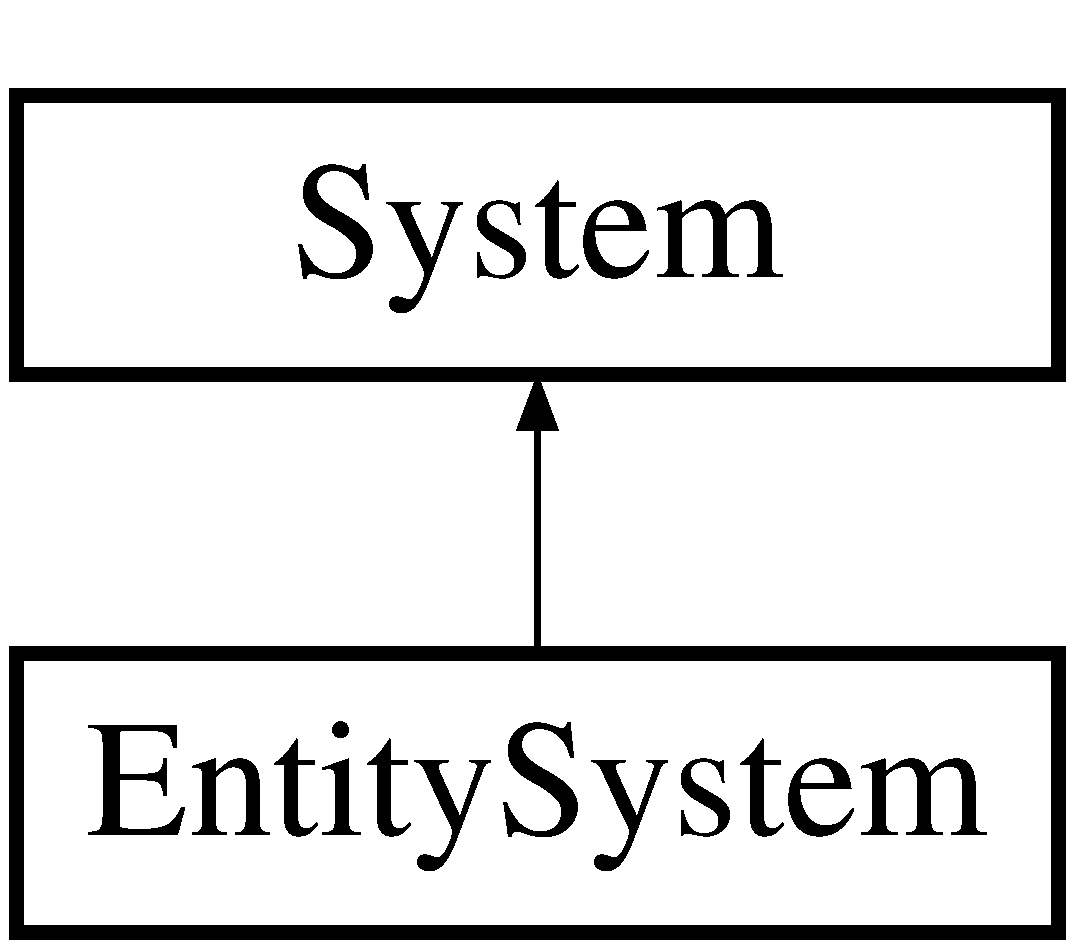
\includegraphics[height=2.000000cm]{class_entity_system}
\end{center}
\end{figure}
\subsection*{Public Member Functions}
\begin{DoxyCompactItemize}
\item 
\hyperlink{class_entity_system_a2bf6f7d3c7b6b7e02c8cc3dd454e9ab1}{Entity\+System} (Ogre\+::\+Scene\+Manager \&)
\begin{DoxyCompactList}\small\item\em Constructor. \end{DoxyCompactList}\item 
\hyperlink{class_entity_system_a8b34e0963a5231a3cda81442771318fb}{$\sim$\+Entity\+System} ()=default
\begin{DoxyCompactList}\small\item\em Destructor. \end{DoxyCompactList}\item 
void \hyperlink{class_entity_system_aa51808181d7c66baea07cec41c17b4cd}{update} (tdt\+::real) override
\begin{DoxyCompactList}\small\item\em Checks for entities with no components and if any are found, deletes them. \end{DoxyCompactList}\item 
tdt\+::uint \hyperlink{class_entity_system_adfb0a9adc4f2d4273d6cbf69d948f23c}{get\+\_\+new\+\_\+id} ()
\begin{DoxyCompactList}\small\item\em Returns first available entity id. \end{DoxyCompactList}\item 
void \hyperlink{class_entity_system_acf6c4ffcec1a74b1f3db6636489a7217}{cleanup} ()
\begin{DoxyCompactList}\small\item\em Removes all entities that have no components and individual components marked for deletion from their entities (this is used so that the Lua code does not delete an entity/a component from a container while C++ iterates over it). \end{DoxyCompactList}\item 
tdt\+::uint \hyperlink{class_entity_system_ac283fa8ea0e3755ad2b267010a7fd6c2}{create\+\_\+entity} (const std\+::string \&=\char`\"{}\char`\"{}, const Ogre\+::\+Vector3 \&=Ogre\+::\+Vector3\{0.f, 0.f, 0.f\})
\begin{DoxyCompactList}\small\item\em Creates a new entity from a blueprint. \end{DoxyCompactList}\item 
const std\+::map$<$ tdt\+::uint, std\+::bitset$<$ Component\+::count $>$ $>$ \& \hyperlink{class_entity_system_aaa1035152c890ca73f47d300d6377498}{get\+\_\+component\+\_\+list} () const 
\begin{DoxyCompactList}\small\item\em Breif\+: Returns const reference to the component list, so that it can be used to iterate over all entities. \end{DoxyCompactList}\item 
{\footnotesize template$<$typename C\+O\+MP $>$ }\\bool \hyperlink{class_entity_system_a0f079d475b904a1a48bce63b4c7d64cd}{has\+\_\+component} (tdt\+::uint id)
\begin{DoxyCompactList}\small\item\em Tests whether a given entity has a component specialized by the template argument. \end{DoxyCompactList}\item 
bool \hyperlink{class_entity_system_a80122f961940fce5ce2493966770b234}{has\+\_\+component} (tdt\+::uint, tdt\+::uint) const 
\begin{DoxyCompactList}\small\item\em Tests whether a given entity has a component of a given type (used from Lua as it cannot use templates). \end{DoxyCompactList}\item 
{\footnotesize template$<$typename C\+O\+MP $>$ }\\C\+O\+MP $\ast$ \hyperlink{class_entity_system_ad9610ae9a595fc16e8f545cf752ee4f0}{get\+\_\+component} (tdt\+::uint id)
\begin{DoxyCompactList}\small\item\em Returns a bool-\/component pointer pair, in which the first bool member determines if the component was found and the second is a pointer to the component. \end{DoxyCompactList}\item 
{\footnotesize template$<$typename C\+O\+MP $>$ }\\void \hyperlink{class_entity_system_aea3df5c0dc93e72513914cdbbeb2a613}{set\+\_\+component} (tdt\+::uint id, C\+O\+MP comp)
\begin{DoxyCompactList}\small\item\em Changes a component (type specified by template argument) of and entity or assigns a new component it that entity didn\textquotesingle{}t have it. \end{DoxyCompactList}\item 
{\footnotesize template$<$typename C\+O\+MP $>$ }\\std\+::map$<$ tdt\+::uint, C\+O\+MP $>$ \& \hyperlink{class_entity_system_ab2bacfe1a7fa117764850f60ead892df}{get\+\_\+component\+\_\+container} ()
\begin{DoxyCompactList}\small\item\em Returns the map associated with the component specified by the template argument. \end{DoxyCompactList}\item 
{\footnotesize template$<$typename C\+O\+MP $>$ }\\void \hyperlink{class_entity_system_a556ec8504fcdd38125b0aaa5245aee20}{add\+\_\+component} (tdt\+::uint id)
\begin{DoxyCompactList}\small\item\em Adds a components to the given enetity using it\textquotesingle{}s default constructor (all values have to be set afterwards). \end{DoxyCompactList}\item 
void \hyperlink{class_entity_system_a6e392f209dbdb990cd1d292a32f5eef2}{add\+\_\+component} (tdt\+::uint, int)
\begin{DoxyCompactList}\small\item\em Allows to add a component based on it\textquotesingle{}s ID. \end{DoxyCompactList}\item 
{\footnotesize template$<$typename C\+O\+MP $>$ }\\void \hyperlink{class_entity_system_ad10b62b1ac279603a3cfca317ed9e079}{delete\+\_\+component} (tdt\+::uint id)
\begin{DoxyCompactList}\small\item\em Marks a component (specified by template argument) for given entity for deletion. \end{DoxyCompactList}\item 
void \hyperlink{class_entity_system_ae60c40dddce4f87862e3973b7869b684}{delete\+\_\+component} (tdt\+::uint, int)
\begin{DoxyCompactList}\small\item\em Allows to enqueue a component for deletion based on it\textquotesingle{}s ID. \end{DoxyCompactList}\item 
void \hyperlink{class_entity_system_ab125a824fcafbf43f60250ecd156b421}{register\+\_\+entity} (const std\+::string \&)
\begin{DoxyCompactList}\small\item\em Registers an entity that has been loaded from a Lua script. \end{DoxyCompactList}\item 
std\+::set$<$ std\+::string $>$ \& \hyperlink{class_entity_system_a205a1ec0b7919409c99996d4f38660a6}{get\+\_\+registered\+\_\+entities} ()
\begin{DoxyCompactList}\small\item\em Returns a reference to the set containing all entity tables registered during the game\textquotesingle{}s runtime. \end{DoxyCompactList}\item 
bool \hyperlink{class_entity_system_a55067af795708645b34ca4586208d95c}{exists} (tdt\+::uint) const 
\begin{DoxyCompactList}\small\item\em Checks if a given entity exists and returns true if it does, false otherwise. \end{DoxyCompactList}\item 
Ogre\+::\+Scene\+Manager \& \hyperlink{class_entity_system_ab3fdbf9ba452c2dab05221f007a63602}{get\+\_\+scene\+\_\+manager} ()
\begin{DoxyCompactList}\small\item\em Returns a reference to the scene manager all entities of this system are attached to (if they have a graphics component). \end{DoxyCompactList}\item 
void \hyperlink{class_entity_system_add914f62bb89bd8cbbd53d46dbd26875}{delete\+\_\+entities} ()
\begin{DoxyCompactList}\small\item\em Deletes all entities int the game, used before loading a new game. \end{DoxyCompactList}\item 
{\footnotesize template$<$$>$ }\\std\+::map$<$ tdt\+::uint, \hyperlink{struct_physics_component}{Physics\+Component} $>$ \& \hyperlink{class_entity_system_aff2e00095e3d492861180202c45ee477}{get\+\_\+component\+\_\+container} ()
\begin{DoxyCompactList}\small\item\em Specializations of the \hyperlink{class_entity_system_ab2bacfe1a7fa117764850f60ead892df}{Entity\+System\+::get\+\_\+component\+\_\+container} method. \end{DoxyCompactList}\item 
{\footnotesize template$<$$>$ }\\std\+::map$<$ tdt\+::uint, \hyperlink{struct_health_component}{Health\+Component} $>$ \& {\bfseries get\+\_\+component\+\_\+container} ()\hypertarget{class_entity_system_a508eed877d281573b043faf930d7d342}{}\label{class_entity_system_a508eed877d281573b043faf930d7d342}

\item 
{\footnotesize template$<$$>$ }\\std\+::map$<$ tdt\+::uint, \hyperlink{struct_a_i_component}{A\+I\+Component} $>$ \& {\bfseries get\+\_\+component\+\_\+container} ()\hypertarget{class_entity_system_a961905fcd206dc5569a676e880841ca2}{}\label{class_entity_system_a961905fcd206dc5569a676e880841ca2}

\item 
{\footnotesize template$<$$>$ }\\std\+::map$<$ tdt\+::uint, \hyperlink{struct_graphics_component}{Graphics\+Component} $>$ \& {\bfseries get\+\_\+component\+\_\+container} ()\hypertarget{class_entity_system_a9909afda5535746578bccefe53aa5c34}{}\label{class_entity_system_a9909afda5535746578bccefe53aa5c34}

\item 
{\footnotesize template$<$$>$ }\\std\+::map$<$ tdt\+::uint, \hyperlink{struct_movement_component}{Movement\+Component} $>$ \& {\bfseries get\+\_\+component\+\_\+container} ()\hypertarget{class_entity_system_af5f2dbc119c055782ebd1106660008c3}{}\label{class_entity_system_af5f2dbc119c055782ebd1106660008c3}

\item 
{\footnotesize template$<$$>$ }\\std\+::map$<$ tdt\+::uint, \hyperlink{struct_combat_component}{Combat\+Component} $>$ \& {\bfseries get\+\_\+component\+\_\+container} ()\hypertarget{class_entity_system_a539a0d84d6a529fedc3907bd27a5c6d0}{}\label{class_entity_system_a539a0d84d6a529fedc3907bd27a5c6d0}

\item 
{\footnotesize template$<$$>$ }\\std\+::map$<$ tdt\+::uint, \hyperlink{struct_event_component}{Event\+Component} $>$ \& {\bfseries get\+\_\+component\+\_\+container} ()\hypertarget{class_entity_system_a1bf83e12fffdab7688d5ee22dda797e6}{}\label{class_entity_system_a1bf83e12fffdab7688d5ee22dda797e6}

\item 
{\footnotesize template$<$$>$ }\\std\+::map$<$ tdt\+::uint, \hyperlink{struct_input_component}{Input\+Component} $>$ \& {\bfseries get\+\_\+component\+\_\+container} ()\hypertarget{class_entity_system_af4df13ed73cc7bf18a4882c5ab6dcdcc}{}\label{class_entity_system_af4df13ed73cc7bf18a4882c5ab6dcdcc}

\item 
{\footnotesize template$<$$>$ }\\std\+::map$<$ tdt\+::uint, \hyperlink{struct_time_component}{Time\+Component} $>$ \& {\bfseries get\+\_\+component\+\_\+container} ()\hypertarget{class_entity_system_aeada2412672fbea2b7a914e2d3b30a2d}{}\label{class_entity_system_aeada2412672fbea2b7a914e2d3b30a2d}

\item 
{\footnotesize template$<$$>$ }\\std\+::map$<$ tdt\+::uint, \hyperlink{struct_mana_component}{Mana\+Component} $>$ \& {\bfseries get\+\_\+component\+\_\+container} ()\hypertarget{class_entity_system_a9ca93121683f21ad2046c2a208922d09}{}\label{class_entity_system_a9ca93121683f21ad2046c2a208922d09}

\item 
{\footnotesize template$<$$>$ }\\std\+::map$<$ tdt\+::uint, \hyperlink{struct_spell_component}{Spell\+Component} $>$ \& {\bfseries get\+\_\+component\+\_\+container} ()\hypertarget{class_entity_system_ac406af2b870d1a2615b134c391ad5099}{}\label{class_entity_system_ac406af2b870d1a2615b134c391ad5099}

\item 
{\footnotesize template$<$$>$ }\\std\+::map$<$ tdt\+::uint, \hyperlink{struct_production_component}{Production\+Component} $>$ \& {\bfseries get\+\_\+component\+\_\+container} ()\hypertarget{class_entity_system_a96157aaaab85d53a67996908b985d3d5}{}\label{class_entity_system_a96157aaaab85d53a67996908b985d3d5}

\item 
{\footnotesize template$<$$>$ }\\std\+::map$<$ tdt\+::uint, \hyperlink{struct_grid_node_component}{Grid\+Node\+Component} $>$ \& {\bfseries get\+\_\+component\+\_\+container} ()\hypertarget{class_entity_system_a573199f54220d256f634d096d56f4340}{}\label{class_entity_system_a573199f54220d256f634d096d56f4340}

\item 
{\footnotesize template$<$$>$ }\\std\+::map$<$ tdt\+::uint, \hyperlink{struct_product_component}{Product\+Component} $>$ \& {\bfseries get\+\_\+component\+\_\+container} ()\hypertarget{class_entity_system_ac32a639180e04c61e378c8ae204f3b7a}{}\label{class_entity_system_ac32a639180e04c61e378c8ae204f3b7a}

\item 
{\footnotesize template$<$$>$ }\\std\+::map$<$ tdt\+::uint, \hyperlink{struct_pathfinding_component}{Pathfinding\+Component} $>$ \& {\bfseries get\+\_\+component\+\_\+container} ()\hypertarget{class_entity_system_aed11982a65e630b80142c2beda45da8b}{}\label{class_entity_system_aed11982a65e630b80142c2beda45da8b}

\item 
{\footnotesize template$<$$>$ }\\std\+::map$<$ tdt\+::uint, \hyperlink{struct_task_component}{Task\+Component} $>$ \& {\bfseries get\+\_\+component\+\_\+container} ()\hypertarget{class_entity_system_a19a63bfab77a3f46c139729e3b24d0fb}{}\label{class_entity_system_a19a63bfab77a3f46c139729e3b24d0fb}

\item 
{\footnotesize template$<$$>$ }\\std\+::map$<$ tdt\+::uint, \hyperlink{struct_task_handler_component}{Task\+Handler\+Component} $>$ \& {\bfseries get\+\_\+component\+\_\+container} ()\hypertarget{class_entity_system_a0d719edae805faa82867fd22b25e29c8}{}\label{class_entity_system_a0d719edae805faa82867fd22b25e29c8}

\item 
{\footnotesize template$<$$>$ }\\std\+::map$<$ tdt\+::uint, \hyperlink{struct_structure_component}{Structure\+Component} $>$ \& {\bfseries get\+\_\+component\+\_\+container} ()\hypertarget{class_entity_system_a92e8154678c984c767a0e4a6ad551d9f}{}\label{class_entity_system_a92e8154678c984c767a0e4a6ad551d9f}

\item 
{\footnotesize template$<$$>$ }\\std\+::map$<$ tdt\+::uint, \hyperlink{struct_homing_component}{Homing\+Component} $>$ \& {\bfseries get\+\_\+component\+\_\+container} ()\hypertarget{class_entity_system_adfa0ce8b0c3fc1b6f1458a0d4627e31e}{}\label{class_entity_system_adfa0ce8b0c3fc1b6f1458a0d4627e31e}

\item 
{\footnotesize template$<$$>$ }\\std\+::map$<$ tdt\+::uint, \hyperlink{struct_event_handler_component}{Event\+Handler\+Component} $>$ \& {\bfseries get\+\_\+component\+\_\+container} ()\hypertarget{class_entity_system_a7d53589e27f0dded16549db53cc0e217}{}\label{class_entity_system_a7d53589e27f0dded16549db53cc0e217}

\item 
{\footnotesize template$<$$>$ }\\std\+::map$<$ tdt\+::uint, \hyperlink{struct_destructor_component}{Destructor\+Component} $>$ \& {\bfseries get\+\_\+component\+\_\+container} ()\hypertarget{class_entity_system_a973f9887b478d19017f4acbe16741054}{}\label{class_entity_system_a973f9887b478d19017f4acbe16741054}

\item 
{\footnotesize template$<$$>$ }\\std\+::map$<$ tdt\+::uint, \hyperlink{struct_gold_component}{Gold\+Component} $>$ \& {\bfseries get\+\_\+component\+\_\+container} ()\hypertarget{class_entity_system_af9586207497be5f663aa009c940d780c}{}\label{class_entity_system_af9586207497be5f663aa009c940d780c}

\item 
{\footnotesize template$<$$>$ }\\std\+::map$<$ tdt\+::uint, \hyperlink{struct_faction_component}{Faction\+Component} $>$ \& {\bfseries get\+\_\+component\+\_\+container} ()\hypertarget{class_entity_system_acd9c209334726b9dd77de42d9b612a8c}{}\label{class_entity_system_acd9c209334726b9dd77de42d9b612a8c}

\item 
{\footnotesize template$<$$>$ }\\std\+::map$<$ tdt\+::uint, \hyperlink{struct_price_component}{Price\+Component} $>$ \& {\bfseries get\+\_\+component\+\_\+container} ()\hypertarget{class_entity_system_a085928660036f87f38a7622b0e381706}{}\label{class_entity_system_a085928660036f87f38a7622b0e381706}

\item 
{\footnotesize template$<$$>$ }\\std\+::map$<$ tdt\+::uint, \hyperlink{struct_align_component}{Align\+Component} $>$ \& {\bfseries get\+\_\+component\+\_\+container} ()\hypertarget{class_entity_system_a58ab65cb9e0a2f737c7b64e2c873eb8f}{}\label{class_entity_system_a58ab65cb9e0a2f737c7b64e2c873eb8f}

\item 
{\footnotesize template$<$$>$ }\\std\+::map$<$ tdt\+::uint, \hyperlink{struct_mine_component}{Mine\+Component} $>$ \& {\bfseries get\+\_\+component\+\_\+container} ()\hypertarget{class_entity_system_ab877cdb98f2d76e5e42d3bd7f632b980}{}\label{class_entity_system_ab877cdb98f2d76e5e42d3bd7f632b980}

\item 
{\footnotesize template$<$$>$ }\\std\+::map$<$ tdt\+::uint, \hyperlink{struct_mana_crystal_component}{Mana\+Crystal\+Component} $>$ \& {\bfseries get\+\_\+component\+\_\+container} ()\hypertarget{class_entity_system_a723cdf78d9ac16489a2d74515d30bb89}{}\label{class_entity_system_a723cdf78d9ac16489a2d74515d30bb89}

\item 
{\footnotesize template$<$$>$ }\\std\+::map$<$ tdt\+::uint, \hyperlink{struct_on_hit_component}{On\+Hit\+Component} $>$ \& {\bfseries get\+\_\+component\+\_\+container} ()\hypertarget{class_entity_system_a417f0ec395e909bf4f25f229b5c75708}{}\label{class_entity_system_a417f0ec395e909bf4f25f229b5c75708}

\item 
{\footnotesize template$<$$>$ }\\std\+::map$<$ tdt\+::uint, \hyperlink{struct_constructor_component}{Constructor\+Component} $>$ \& {\bfseries get\+\_\+component\+\_\+container} ()\hypertarget{class_entity_system_aceca061a4a029c3098161812283cafd3}{}\label{class_entity_system_aceca061a4a029c3098161812283cafd3}

\item 
{\footnotesize template$<$$>$ }\\std\+::map$<$ tdt\+::uint, \hyperlink{struct_trigger_component}{Trigger\+Component} $>$ \& {\bfseries get\+\_\+component\+\_\+container} ()\hypertarget{class_entity_system_a1e739ee1344c165ad6c4fc367012fcb7}{}\label{class_entity_system_a1e739ee1344c165ad6c4fc367012fcb7}

\item 
{\footnotesize template$<$$>$ }\\std\+::map$<$ tdt\+::uint, \hyperlink{struct_upgrade_component}{Upgrade\+Component} $>$ \& {\bfseries get\+\_\+component\+\_\+container} ()\hypertarget{class_entity_system_ae6cb26520283845d6252246a1036bf11}{}\label{class_entity_system_ae6cb26520283845d6252246a1036bf11}

\item 
{\footnotesize template$<$$>$ }\\std\+::map$<$ tdt\+::uint, \hyperlink{struct_notification_component}{Notification\+Component} $>$ \& {\bfseries get\+\_\+component\+\_\+container} ()\hypertarget{class_entity_system_ad5b9130b15cd48cfde11e53ee7eb707f}{}\label{class_entity_system_ad5b9130b15cd48cfde11e53ee7eb707f}

\item 
{\footnotesize template$<$$>$ }\\std\+::map$<$ tdt\+::uint, \hyperlink{struct_explosion_component}{Explosion\+Component} $>$ \& {\bfseries get\+\_\+component\+\_\+container} ()\hypertarget{class_entity_system_afac3210cc029aaf03ae43ebc1231fbd9}{}\label{class_entity_system_afac3210cc029aaf03ae43ebc1231fbd9}

\item 
{\footnotesize template$<$$>$ }\\std\+::map$<$ tdt\+::uint, \hyperlink{struct_limited_life_span_component}{Limited\+Life\+Span\+Component} $>$ \& {\bfseries get\+\_\+component\+\_\+container} ()\hypertarget{class_entity_system_a3ed3367fad2ed4db1e756d6db9d1aa71}{}\label{class_entity_system_a3ed3367fad2ed4db1e756d6db9d1aa71}

\item 
{\footnotesize template$<$$>$ }\\std\+::map$<$ tdt\+::uint, \hyperlink{struct_name_component}{Name\+Component} $>$ \& {\bfseries get\+\_\+component\+\_\+container} ()\hypertarget{class_entity_system_a7bc07dda74ab1a10fbde39e0f7536c74}{}\label{class_entity_system_a7bc07dda74ab1a10fbde39e0f7536c74}

\item 
{\footnotesize template$<$$>$ }\\std\+::map$<$ tdt\+::uint, \hyperlink{struct_experience_value_component}{Experience\+Value\+Component} $>$ \& {\bfseries get\+\_\+component\+\_\+container} ()\hypertarget{class_entity_system_ab56d27de7ff71878e26b4214d75af1b3}{}\label{class_entity_system_ab56d27de7ff71878e26b4214d75af1b3}

\item 
{\footnotesize template$<$$>$ }\\std\+::map$<$ tdt\+::uint, \hyperlink{struct_light_component}{Light\+Component} $>$ \& {\bfseries get\+\_\+component\+\_\+container} ()\hypertarget{class_entity_system_a55cb72f54ca005f494316df828de118a}{}\label{class_entity_system_a55cb72f54ca005f494316df828de118a}

\item 
{\footnotesize template$<$$>$ }\\std\+::map$<$ tdt\+::uint, \hyperlink{struct_command_component}{Command\+Component} $>$ \& {\bfseries get\+\_\+component\+\_\+container} ()\hypertarget{class_entity_system_a3b84416a3c422656f9daa09535b836b9}{}\label{class_entity_system_a3b84416a3c422656f9daa09535b836b9}

\item 
{\footnotesize template$<$$>$ }\\std\+::map$<$ tdt\+::uint, \hyperlink{struct_counter_component}{Counter\+Component} $>$ \& {\bfseries get\+\_\+component\+\_\+container} ()\hypertarget{class_entity_system_a8841eb6b81a9be95566ff0eebcb1121d}{}\label{class_entity_system_a8841eb6b81a9be95566ff0eebcb1121d}

\item 
{\footnotesize template$<$$>$ }\\std\+::map$<$ tdt\+::uint, \hyperlink{struct_portal_component}{Portal\+Component} $>$ \& {\bfseries get\+\_\+component\+\_\+container} ()\hypertarget{class_entity_system_a23789f4f49cd2b2ec424034efeeabe91}{}\label{class_entity_system_a23789f4f49cd2b2ec424034efeeabe91}

\end{DoxyCompactItemize}
\subsection*{Public Attributes}
\begin{DoxyCompactItemize}
\item 
std\+::string \hyperlink{class_entity_system_a41e0561691509c232c26dc78c819c74e}{N\+O\+\_\+\+B\+L\+U\+E\+P\+R\+I\+NT} \{\char`\"{}E\+R\+R\+OR\char`\"{}\}
\begin{DoxyCompactList}\small\item\em Used in helpers when no component exists and we still need to return the blueprint name (in this case the E\+R\+R\+OR blueprint) by reference. \end{DoxyCompactList}\item 
std\+::array$<$ std\+::string, 3 $>$ \hyperlink{class_entity_system_a64eff1a78f8685a3b8319b5219381963}{F\+A\+C\+T\+I\+O\+N\+\_\+\+N\+A\+ME} \{\char`\"{}F\+R\+I\+E\+N\+D\+LY\char`\"{}, \char`\"{}E\+N\+E\+MY\char`\"{}, \char`\"{}N\+E\+U\+T\+R\+AL\char`\"{}\}
\begin{DoxyCompactList}\small\item\em Used in when translating the faction enum to a string in the \hyperlink{namespace_faction_helper}{Faction\+Helper}. \end{DoxyCompactList}\end{DoxyCompactItemize}
\subsection*{Private Types}
\begin{DoxyCompactItemize}
\item 
typedef void(Entity\+System\+::$\ast$ {\bfseries Loader\+Func\+Ptr}) (tdt\+::uint, const std\+::string \&)\hypertarget{class_entity_system_ab03b379651ef1bf67979d7b7fc92159f}{}\label{class_entity_system_ab03b379651ef1bf67979d7b7fc92159f}

\item 
typedef void(Entity\+System\+::$\ast$ {\bfseries Adder\+Func\+Ptr}) (tdt\+::uint)\hypertarget{class_entity_system_a79cd6b4f2069db9cb8385aa10ac5e3f3}{}\label{class_entity_system_a79cd6b4f2069db9cb8385aa10ac5e3f3}

\item 
typedef void(Entity\+System\+::$\ast$ {\bfseries Deleter\+Func\+Ptr}) (tdt\+::uint)\hypertarget{class_entity_system_aa157465c64a590da2c678dde38993d97}{}\label{class_entity_system_aa157465c64a590da2c678dde38993d97}

\item 
typedef void(Entity\+System\+::$\ast$ {\bfseries Immediate\+Deleter\+Func\+Ptr}) (tdt\+::uint)\hypertarget{class_entity_system_af8220281ae12f27126e4203d922a2931}{}\label{class_entity_system_af8220281ae12f27126e4203d922a2931}

\end{DoxyCompactItemize}
\subsection*{Private Member Functions}
\begin{DoxyCompactItemize}
\item 
{\footnotesize template$<$typename C\+O\+MP $>$ }\\void \hyperlink{class_entity_system_ac2d122f65e967b51cc37227b5dd0a7fe}{load\+\_\+component} (tdt\+::uint id, const std\+::string \&table\+\_\+name)
\begin{DoxyCompactList}\small\item\em Loads a component from a Lua script. \end{DoxyCompactList}\item 
void \hyperlink{class_entity_system_a4ecd6127995602d98736cd1cf5799c11}{destroy\+\_\+entity} (tdt\+::uint)
\begin{DoxyCompactList}\small\item\em Removes an entity from the system, thus killing/destroying it. \end{DoxyCompactList}\item 
{\footnotesize template$<$typename C\+O\+MP $>$ }\\void \hyperlink{class_entity_system_ad52fb0d17a2fbd056ffd455b6a1171c7}{delete\+\_\+component\+\_\+now} (tdt\+::uint id)
\begin{DoxyCompactList}\small\item\em Deletes a component. \end{DoxyCompactList}\item 
void \hyperlink{class_entity_system_a99ae4bc51a7e97da9bb8ebb56443b70e}{delete\+\_\+component\+\_\+now} (tdt\+::uint, int)
\begin{DoxyCompactList}\small\item\em Deletes a component. \end{DoxyCompactList}\item 
void \hyperlink{class_entity_system_a54c64fce9cd3fe9f1d2502f0d2b4a93e}{init\+\_\+function\+\_\+arrays} ()
\begin{DoxyCompactList}\small\item\em Initializes all arrays holding pointers to the component manipulating methods. \end{DoxyCompactList}\item 
{\footnotesize template$<$typename C\+O\+MP $>$ }\\void \hyperlink{class_entity_system_abbe94182987541e7047ee1a8fa3388b7}{clean\+\_\+up\+\_\+component} (tdt\+::uint)
\begin{DoxyCompactList}\small\item\em Deletes all necessary data when destroying a component (like Ogre related objects, other entities, tasks etc.). \end{DoxyCompactList}\item 
{\footnotesize template$<$$>$ }\\void \hyperlink{class_entity_system_ac8eead7736efd2ae728661f901142b27}{load\+\_\+component} (tdt\+::uint id, const std\+::string \&table\+\_\+name)
\begin{DoxyCompactList}\small\item\em Specializations of the \hyperlink{class_entity_system_ac2d122f65e967b51cc37227b5dd0a7fe}{Entity\+System\+::load\+\_\+component} method. \end{DoxyCompactList}\item 
{\footnotesize template$<$$>$ }\\void {\bfseries load\+\_\+component} (tdt\+::uint id, const std\+::string \&table\+\_\+name)\hypertarget{class_entity_system_ac8eead7736efd2ae728661f901142b27}{}\label{class_entity_system_ac8eead7736efd2ae728661f901142b27}

\item 
{\footnotesize template$<$$>$ }\\void {\bfseries load\+\_\+component} (tdt\+::uint id, const std\+::string \&table\+\_\+name)\hypertarget{class_entity_system_ac8eead7736efd2ae728661f901142b27}{}\label{class_entity_system_ac8eead7736efd2ae728661f901142b27}

\item 
{\footnotesize template$<$$>$ }\\void {\bfseries load\+\_\+component} (tdt\+::uint id, const std\+::string \&table\+\_\+name)\hypertarget{class_entity_system_ac8eead7736efd2ae728661f901142b27}{}\label{class_entity_system_ac8eead7736efd2ae728661f901142b27}

\item 
{\footnotesize template$<$$>$ }\\void {\bfseries load\+\_\+component} (tdt\+::uint id, const std\+::string \&table\+\_\+name)\hypertarget{class_entity_system_ac8eead7736efd2ae728661f901142b27}{}\label{class_entity_system_ac8eead7736efd2ae728661f901142b27}

\item 
{\footnotesize template$<$$>$ }\\void {\bfseries load\+\_\+component} (tdt\+::uint id, const std\+::string \&table\+\_\+name)\hypertarget{class_entity_system_ac8eead7736efd2ae728661f901142b27}{}\label{class_entity_system_ac8eead7736efd2ae728661f901142b27}

\item 
{\footnotesize template$<$$>$ }\\void {\bfseries load\+\_\+component} (tdt\+::uint id, const std\+::string \&table\+\_\+name)\hypertarget{class_entity_system_ac8eead7736efd2ae728661f901142b27}{}\label{class_entity_system_ac8eead7736efd2ae728661f901142b27}

\item 
{\footnotesize template$<$$>$ }\\void {\bfseries load\+\_\+component} (tdt\+::uint id, const std\+::string \&table\+\_\+name)\hypertarget{class_entity_system_ac8eead7736efd2ae728661f901142b27}{}\label{class_entity_system_ac8eead7736efd2ae728661f901142b27}

\item 
{\footnotesize template$<$$>$ }\\void {\bfseries load\+\_\+component} (tdt\+::uint id, const std\+::string \&table\+\_\+name)\hypertarget{class_entity_system_ac8eead7736efd2ae728661f901142b27}{}\label{class_entity_system_ac8eead7736efd2ae728661f901142b27}

\item 
{\footnotesize template$<$$>$ }\\void {\bfseries load\+\_\+component} (tdt\+::uint id, const std\+::string \&table\+\_\+name)\hypertarget{class_entity_system_ac8eead7736efd2ae728661f901142b27}{}\label{class_entity_system_ac8eead7736efd2ae728661f901142b27}

\item 
{\footnotesize template$<$$>$ }\\void {\bfseries load\+\_\+component} (tdt\+::uint id, const std\+::string \&table\+\_\+name)\hypertarget{class_entity_system_ac8eead7736efd2ae728661f901142b27}{}\label{class_entity_system_ac8eead7736efd2ae728661f901142b27}

\item 
{\footnotesize template$<$$>$ }\\void {\bfseries load\+\_\+component} (tdt\+::uint id, const std\+::string \&table\+\_\+name)\hypertarget{class_entity_system_ac8eead7736efd2ae728661f901142b27}{}\label{class_entity_system_ac8eead7736efd2ae728661f901142b27}

\item 
{\footnotesize template$<$$>$ }\\void {\bfseries load\+\_\+component} (tdt\+::uint id, const std\+::string \&table\+\_\+name)\hypertarget{class_entity_system_ac8eead7736efd2ae728661f901142b27}{}\label{class_entity_system_ac8eead7736efd2ae728661f901142b27}

\item 
{\footnotesize template$<$$>$ }\\void {\bfseries load\+\_\+component} (tdt\+::uint id, const std\+::string \&table\+\_\+name)\hypertarget{class_entity_system_ac8eead7736efd2ae728661f901142b27}{}\label{class_entity_system_ac8eead7736efd2ae728661f901142b27}

\item 
{\footnotesize template$<$$>$ }\\void {\bfseries load\+\_\+component} (tdt\+::uint id, const std\+::string \&table\+\_\+name)\hypertarget{class_entity_system_ac8eead7736efd2ae728661f901142b27}{}\label{class_entity_system_ac8eead7736efd2ae728661f901142b27}

\item 
{\footnotesize template$<$$>$ }\\void {\bfseries load\+\_\+component} (tdt\+::uint id, const std\+::string \&table\+\_\+name)\hypertarget{class_entity_system_ac8eead7736efd2ae728661f901142b27}{}\label{class_entity_system_ac8eead7736efd2ae728661f901142b27}

\item 
{\footnotesize template$<$$>$ }\\void {\bfseries load\+\_\+component} (tdt\+::uint id, const std\+::string \&table\+\_\+name)\hypertarget{class_entity_system_ac8eead7736efd2ae728661f901142b27}{}\label{class_entity_system_ac8eead7736efd2ae728661f901142b27}

\item 
{\footnotesize template$<$$>$ }\\void {\bfseries load\+\_\+component} (tdt\+::uint id, const std\+::string \&table\+\_\+name)\hypertarget{class_entity_system_ac8eead7736efd2ae728661f901142b27}{}\label{class_entity_system_ac8eead7736efd2ae728661f901142b27}

\item 
{\footnotesize template$<$$>$ }\\void {\bfseries load\+\_\+component} (tdt\+::uint id, const std\+::string \&table\+\_\+name)\hypertarget{class_entity_system_ac8eead7736efd2ae728661f901142b27}{}\label{class_entity_system_ac8eead7736efd2ae728661f901142b27}

\item 
{\footnotesize template$<$$>$ }\\void {\bfseries load\+\_\+component} (tdt\+::uint id, const std\+::string \&table\+\_\+name)\hypertarget{class_entity_system_ac8eead7736efd2ae728661f901142b27}{}\label{class_entity_system_ac8eead7736efd2ae728661f901142b27}

\item 
{\footnotesize template$<$$>$ }\\void {\bfseries load\+\_\+component} (tdt\+::uint id, const std\+::string \&table\+\_\+name)\hypertarget{class_entity_system_ac8eead7736efd2ae728661f901142b27}{}\label{class_entity_system_ac8eead7736efd2ae728661f901142b27}

\item 
{\footnotesize template$<$$>$ }\\void {\bfseries load\+\_\+component} (tdt\+::uint id, const std\+::string \&table\+\_\+name)\hypertarget{class_entity_system_ac8eead7736efd2ae728661f901142b27}{}\label{class_entity_system_ac8eead7736efd2ae728661f901142b27}

\item 
{\footnotesize template$<$$>$ }\\void {\bfseries load\+\_\+component} (tdt\+::uint id, const std\+::string \&table\+\_\+name)\hypertarget{class_entity_system_ac8eead7736efd2ae728661f901142b27}{}\label{class_entity_system_ac8eead7736efd2ae728661f901142b27}

\item 
{\footnotesize template$<$$>$ }\\void {\bfseries load\+\_\+component} (tdt\+::uint id, const std\+::string \&table\+\_\+name)\hypertarget{class_entity_system_ac8eead7736efd2ae728661f901142b27}{}\label{class_entity_system_ac8eead7736efd2ae728661f901142b27}

\item 
{\footnotesize template$<$$>$ }\\void {\bfseries load\+\_\+component} (tdt\+::uint id, const std\+::string \&table\+\_\+name)\hypertarget{class_entity_system_ac8eead7736efd2ae728661f901142b27}{}\label{class_entity_system_ac8eead7736efd2ae728661f901142b27}

\item 
{\footnotesize template$<$$>$ }\\void {\bfseries load\+\_\+component} (tdt\+::uint id, const std\+::string \&table\+\_\+name)\hypertarget{class_entity_system_ac8eead7736efd2ae728661f901142b27}{}\label{class_entity_system_ac8eead7736efd2ae728661f901142b27}

\item 
{\footnotesize template$<$$>$ }\\void {\bfseries load\+\_\+component} (tdt\+::uint id, const std\+::string \&table\+\_\+name)\hypertarget{class_entity_system_ac8eead7736efd2ae728661f901142b27}{}\label{class_entity_system_ac8eead7736efd2ae728661f901142b27}

\item 
{\footnotesize template$<$$>$ }\\void {\bfseries load\+\_\+component} (tdt\+::uint id, const std\+::string \&table\+\_\+name)\hypertarget{class_entity_system_ac8eead7736efd2ae728661f901142b27}{}\label{class_entity_system_ac8eead7736efd2ae728661f901142b27}

\item 
{\footnotesize template$<$$>$ }\\void {\bfseries load\+\_\+component} (tdt\+::uint id, const std\+::string \&table\+\_\+name)\hypertarget{class_entity_system_ac8eead7736efd2ae728661f901142b27}{}\label{class_entity_system_ac8eead7736efd2ae728661f901142b27}

\item 
{\footnotesize template$<$$>$ }\\void {\bfseries load\+\_\+component} (tdt\+::uint id, const std\+::string \&table\+\_\+name)\hypertarget{class_entity_system_ac8eead7736efd2ae728661f901142b27}{}\label{class_entity_system_ac8eead7736efd2ae728661f901142b27}

\item 
{\footnotesize template$<$$>$ }\\void {\bfseries load\+\_\+component} (tdt\+::uint id, const std\+::string \&table\+\_\+name)\hypertarget{class_entity_system_ac8eead7736efd2ae728661f901142b27}{}\label{class_entity_system_ac8eead7736efd2ae728661f901142b27}

\item 
{\footnotesize template$<$$>$ }\\void {\bfseries load\+\_\+component} (tdt\+::uint id, const std\+::string \&table\+\_\+name)\hypertarget{class_entity_system_ac8eead7736efd2ae728661f901142b27}{}\label{class_entity_system_ac8eead7736efd2ae728661f901142b27}

\item 
{\footnotesize template$<$$>$ }\\void {\bfseries load\+\_\+component} (tdt\+::uint id, const std\+::string \&table\+\_\+name)\hypertarget{class_entity_system_ac8eead7736efd2ae728661f901142b27}{}\label{class_entity_system_ac8eead7736efd2ae728661f901142b27}

\item 
{\footnotesize template$<$$>$ }\\void {\bfseries load\+\_\+component} (tdt\+::uint id, const std\+::string \&table\+\_\+name)\hypertarget{class_entity_system_ac8eead7736efd2ae728661f901142b27}{}\label{class_entity_system_ac8eead7736efd2ae728661f901142b27}

\item 
{\footnotesize template$<$$>$ }\\void {\bfseries load\+\_\+component} (tdt\+::uint id, const std\+::string \&table\+\_\+name)\hypertarget{class_entity_system_ac8eead7736efd2ae728661f901142b27}{}\label{class_entity_system_ac8eead7736efd2ae728661f901142b27}

\item 
{\footnotesize template$<$$>$ }\\void {\bfseries load\+\_\+component} (tdt\+::uint id, const std\+::string \&table\+\_\+name)\hypertarget{class_entity_system_ac8eead7736efd2ae728661f901142b27}{}\label{class_entity_system_ac8eead7736efd2ae728661f901142b27}

\item 
{\footnotesize template$<$$>$ }\\void {\bfseries load\+\_\+component} (tdt\+::uint id, const std\+::string \&table\+\_\+name)\hypertarget{class_entity_system_ac8eead7736efd2ae728661f901142b27}{}\label{class_entity_system_ac8eead7736efd2ae728661f901142b27}

\item 
{\footnotesize template$<$$>$ }\\void \hyperlink{class_entity_system_a65dfc1efc2561a48999d82377cf22bfa}{clean\+\_\+up\+\_\+component} (tdt\+::uint id)
\begin{DoxyCompactList}\small\item\em Specializations of the \hyperlink{class_entity_system_abbe94182987541e7047ee1a8fa3388b7}{Entity\+System\+::clean\+\_\+up\+\_\+component} method. \end{DoxyCompactList}\item 
{\footnotesize template$<$$>$ }\\void \hyperlink{class_entity_system_a65dfc1efc2561a48999d82377cf22bfa}{clean\+\_\+up\+\_\+component} (tdt\+::uint id)
\item 
{\footnotesize template$<$$>$ }\\void \hyperlink{class_entity_system_a65dfc1efc2561a48999d82377cf22bfa}{clean\+\_\+up\+\_\+component} (tdt\+::uint id)
\item 
{\footnotesize template$<$$>$ }\\void {\bfseries clean\+\_\+up\+\_\+component} (tdt\+::uint id)\hypertarget{class_entity_system_a65dfc1efc2561a48999d82377cf22bfa}{}\label{class_entity_system_a65dfc1efc2561a48999d82377cf22bfa}

\item 
{\footnotesize template$<$$>$ }\\void {\bfseries clean\+\_\+up\+\_\+component} (tdt\+::uint id)\hypertarget{class_entity_system_a65dfc1efc2561a48999d82377cf22bfa}{}\label{class_entity_system_a65dfc1efc2561a48999d82377cf22bfa}

\item 
{\footnotesize template$<$$>$ }\\void {\bfseries clean\+\_\+up\+\_\+component} (tdt\+::uint id)\hypertarget{class_entity_system_a65dfc1efc2561a48999d82377cf22bfa}{}\label{class_entity_system_a65dfc1efc2561a48999d82377cf22bfa}

\item 
{\footnotesize template$<$$>$ }\\void {\bfseries clean\+\_\+up\+\_\+component} (tdt\+::uint id)\hypertarget{class_entity_system_a65dfc1efc2561a48999d82377cf22bfa}{}\label{class_entity_system_a65dfc1efc2561a48999d82377cf22bfa}

\item 
{\footnotesize template$<$$>$ }\\void {\bfseries clean\+\_\+up\+\_\+component} (tdt\+::uint id)\hypertarget{class_entity_system_a65dfc1efc2561a48999d82377cf22bfa}{}\label{class_entity_system_a65dfc1efc2561a48999d82377cf22bfa}

\end{DoxyCompactItemize}
\subsection*{Private Attributes}
\begin{DoxyCompactItemize}
\item 
std\+::map$<$ tdt\+::uint, std\+::bitset$<$ Component\+::count $>$ $>$ \hyperlink{class_entity_system_a830f1669703edf2e3d6271c3732f8ef5}{entities\+\_\+}
\begin{DoxyCompactList}\small\item\em Contains bitsets describing component availability. \end{DoxyCompactList}\item 
std\+::vector$<$ tdt\+::uint $>$ \hyperlink{class_entity_system_a3b18dc742fb036c9fae1836136b3e115}{to\+\_\+be\+\_\+destroyed\+\_\+}
\begin{DoxyCompactList}\small\item\em Used to mark components or entire entities for removal. \end{DoxyCompactList}\item 
std\+::vector$<$ std\+::pair$<$ tdt\+::uint, int $>$ $>$ {\bfseries components\+\_\+to\+\_\+be\+\_\+removed\+\_\+}\hypertarget{class_entity_system_abacca25b459b880924b38226206257dd}{}\label{class_entity_system_abacca25b459b880924b38226206257dd}

\item 
std\+::map$<$ tdt\+::uint, \hyperlink{struct_physics_component}{Physics\+Component} $>$ \hyperlink{class_entity_system_a6d0a97449d5346dbc389abbedccf06f8}{physics\+\_\+} \{\}
\begin{DoxyCompactList}\small\item\em Contain components specified by the entity ID. \end{DoxyCompactList}\item 
std\+::map$<$ tdt\+::uint, \hyperlink{struct_health_component}{Health\+Component} $>$ {\bfseries health\+\_\+} \{\}\hypertarget{class_entity_system_a10ce033f36068b73c6300a9ac76afc2c}{}\label{class_entity_system_a10ce033f36068b73c6300a9ac76afc2c}

\item 
std\+::map$<$ tdt\+::uint, \hyperlink{struct_a_i_component}{A\+I\+Component} $>$ {\bfseries ai\+\_\+} \{\}\hypertarget{class_entity_system_acaf09bbfa8f91493c7126c93413873ee}{}\label{class_entity_system_acaf09bbfa8f91493c7126c93413873ee}

\item 
std\+::map$<$ tdt\+::uint, \hyperlink{struct_graphics_component}{Graphics\+Component} $>$ {\bfseries graphics\+\_\+} \{\}\hypertarget{class_entity_system_a2c3bda5d6b20ac2e9534c3d3d0eb31e7}{}\label{class_entity_system_a2c3bda5d6b20ac2e9534c3d3d0eb31e7}

\item 
std\+::map$<$ tdt\+::uint, \hyperlink{struct_movement_component}{Movement\+Component} $>$ {\bfseries movement\+\_\+} \{\}\hypertarget{class_entity_system_a72aedf0d22c9eb94bee7a35a01f4932c}{}\label{class_entity_system_a72aedf0d22c9eb94bee7a35a01f4932c}

\item 
std\+::map$<$ tdt\+::uint, \hyperlink{struct_combat_component}{Combat\+Component} $>$ {\bfseries combat\+\_\+} \{\}\hypertarget{class_entity_system_a4ad5edb5ea5966b530758bfd7cbf97b7}{}\label{class_entity_system_a4ad5edb5ea5966b530758bfd7cbf97b7}

\item 
std\+::map$<$ tdt\+::uint, \hyperlink{struct_event_component}{Event\+Component} $>$ {\bfseries event\+\_\+} \{\}\hypertarget{class_entity_system_ae462dcb2ed02716e55ebe7daa30ddefe}{}\label{class_entity_system_ae462dcb2ed02716e55ebe7daa30ddefe}

\item 
std\+::map$<$ tdt\+::uint, \hyperlink{struct_input_component}{Input\+Component} $>$ {\bfseries input\+\_\+} \{\}\hypertarget{class_entity_system_a8b23771e0d57b94a0a9965b9bd962618}{}\label{class_entity_system_a8b23771e0d57b94a0a9965b9bd962618}

\item 
std\+::map$<$ tdt\+::uint, \hyperlink{struct_time_component}{Time\+Component} $>$ {\bfseries time\+\_\+} \{\}\hypertarget{class_entity_system_a2266bb5ccfc3e59dc6cedc2df9d9693f}{}\label{class_entity_system_a2266bb5ccfc3e59dc6cedc2df9d9693f}

\item 
std\+::map$<$ tdt\+::uint, \hyperlink{struct_mana_component}{Mana\+Component} $>$ {\bfseries mana\+\_\+} \{\}\hypertarget{class_entity_system_aaa627f7d263a935948dd478863361b0a}{}\label{class_entity_system_aaa627f7d263a935948dd478863361b0a}

\item 
std\+::map$<$ tdt\+::uint, \hyperlink{struct_spell_component}{Spell\+Component} $>$ {\bfseries spell\+\_\+} \{\}\hypertarget{class_entity_system_ace9c6990c0e158579e4ab9484579a640}{}\label{class_entity_system_ace9c6990c0e158579e4ab9484579a640}

\item 
std\+::map$<$ tdt\+::uint, \hyperlink{struct_production_component}{Production\+Component} $>$ {\bfseries production\+\_\+} \{\}\hypertarget{class_entity_system_aab0d0613a95df77125b0d80079e9a101}{}\label{class_entity_system_aab0d0613a95df77125b0d80079e9a101}

\item 
std\+::map$<$ tdt\+::uint, \hyperlink{struct_grid_node_component}{Grid\+Node\+Component} $>$ {\bfseries grid\+\_\+node\+\_\+} \{\}\hypertarget{class_entity_system_a80611774b556117f69ba3b0376dc0d6e}{}\label{class_entity_system_a80611774b556117f69ba3b0376dc0d6e}

\item 
std\+::map$<$ tdt\+::uint, \hyperlink{struct_product_component}{Product\+Component} $>$ {\bfseries product\+\_\+} \{\}\hypertarget{class_entity_system_a2fcd6980b698066b3c8d3ec039474bce}{}\label{class_entity_system_a2fcd6980b698066b3c8d3ec039474bce}

\item 
std\+::map$<$ tdt\+::uint, \hyperlink{struct_pathfinding_component}{Pathfinding\+Component} $>$ {\bfseries pathfinding\+\_\+} \{\}\hypertarget{class_entity_system_a8948d0cce621c20516541b1a3c6b8c9a}{}\label{class_entity_system_a8948d0cce621c20516541b1a3c6b8c9a}

\item 
std\+::map$<$ tdt\+::uint, \hyperlink{struct_task_component}{Task\+Component} $>$ {\bfseries task\+\_\+} \{\}\hypertarget{class_entity_system_adae3a93692d10e343fc476a59c574ccb}{}\label{class_entity_system_adae3a93692d10e343fc476a59c574ccb}

\item 
std\+::map$<$ tdt\+::uint, \hyperlink{struct_task_handler_component}{Task\+Handler\+Component} $>$ {\bfseries task\+\_\+handler\+\_\+} \{\}\hypertarget{class_entity_system_a238a118b5585f20f179089b4b0c422f2}{}\label{class_entity_system_a238a118b5585f20f179089b4b0c422f2}

\item 
std\+::map$<$ tdt\+::uint, \hyperlink{struct_structure_component}{Structure\+Component} $>$ {\bfseries structure\+\_\+} \{\}\hypertarget{class_entity_system_a3fd7a5df1c05aed80fd7acd7c72dfad6}{}\label{class_entity_system_a3fd7a5df1c05aed80fd7acd7c72dfad6}

\item 
std\+::map$<$ tdt\+::uint, \hyperlink{struct_homing_component}{Homing\+Component} $>$ {\bfseries homing\+\_\+} \{\}\hypertarget{class_entity_system_a60c125a3b5d21c07835db0ed74be0178}{}\label{class_entity_system_a60c125a3b5d21c07835db0ed74be0178}

\item 
std\+::map$<$ tdt\+::uint, \hyperlink{struct_event_handler_component}{Event\+Handler\+Component} $>$ {\bfseries event\+\_\+handler\+\_\+} \{\}\hypertarget{class_entity_system_ab435505f9b51d7f5a668ef98e853b5e1}{}\label{class_entity_system_ab435505f9b51d7f5a668ef98e853b5e1}

\item 
std\+::map$<$ tdt\+::uint, \hyperlink{struct_destructor_component}{Destructor\+Component} $>$ {\bfseries destructor\+\_\+} \{\}\hypertarget{class_entity_system_a255f5a0a573340454d88cb3d373523f3}{}\label{class_entity_system_a255f5a0a573340454d88cb3d373523f3}

\item 
std\+::map$<$ tdt\+::uint, \hyperlink{struct_gold_component}{Gold\+Component} $>$ {\bfseries gold\+\_\+} \{\}\hypertarget{class_entity_system_af7d14e35001c78315710b3c1c13c0cdf}{}\label{class_entity_system_af7d14e35001c78315710b3c1c13c0cdf}

\item 
std\+::map$<$ tdt\+::uint, \hyperlink{struct_faction_component}{Faction\+Component} $>$ {\bfseries faction\+\_\+} \{\}\hypertarget{class_entity_system_afcbd1bd503bb0112b65427867f6411ac}{}\label{class_entity_system_afcbd1bd503bb0112b65427867f6411ac}

\item 
std\+::map$<$ tdt\+::uint, \hyperlink{struct_price_component}{Price\+Component} $>$ {\bfseries price\+\_\+} \{\}\hypertarget{class_entity_system_ae9bc022455b06ea73897ca79a0d73171}{}\label{class_entity_system_ae9bc022455b06ea73897ca79a0d73171}

\item 
std\+::map$<$ tdt\+::uint, \hyperlink{struct_align_component}{Align\+Component} $>$ {\bfseries align\+\_\+} \{\}\hypertarget{class_entity_system_a8dc3fef5f4b6d5c0d386aa84e27e76f9}{}\label{class_entity_system_a8dc3fef5f4b6d5c0d386aa84e27e76f9}

\item 
std\+::map$<$ tdt\+::uint, \hyperlink{struct_mine_component}{Mine\+Component} $>$ {\bfseries mine\+\_\+} \{\}\hypertarget{class_entity_system_a84a91531d0b15c06c9dbe24528e6ce6a}{}\label{class_entity_system_a84a91531d0b15c06c9dbe24528e6ce6a}

\item 
std\+::map$<$ tdt\+::uint, \hyperlink{struct_mana_crystal_component}{Mana\+Crystal\+Component} $>$ {\bfseries mana\+\_\+crystal\+\_\+} \{\}\hypertarget{class_entity_system_a4161310db14b4210aa54a76a8879e3e6}{}\label{class_entity_system_a4161310db14b4210aa54a76a8879e3e6}

\item 
std\+::map$<$ tdt\+::uint, \hyperlink{struct_on_hit_component}{On\+Hit\+Component} $>$ {\bfseries on\+\_\+hit\+\_\+} \{\}\hypertarget{class_entity_system_acb74a0737b50fed58e57e87be1304595}{}\label{class_entity_system_acb74a0737b50fed58e57e87be1304595}

\item 
std\+::map$<$ tdt\+::uint, \hyperlink{struct_constructor_component}{Constructor\+Component} $>$ {\bfseries constructor\+\_\+} \{\}\hypertarget{class_entity_system_a3b4e8a7104f8d780d03ad396778bca35}{}\label{class_entity_system_a3b4e8a7104f8d780d03ad396778bca35}

\item 
std\+::map$<$ tdt\+::uint, \hyperlink{struct_trigger_component}{Trigger\+Component} $>$ {\bfseries trigger\+\_\+} \{\}\hypertarget{class_entity_system_a1bcbfa529cb6b5a0e25dbe47b95aec13}{}\label{class_entity_system_a1bcbfa529cb6b5a0e25dbe47b95aec13}

\item 
std\+::map$<$ tdt\+::uint, \hyperlink{struct_upgrade_component}{Upgrade\+Component} $>$ {\bfseries upgrade\+\_\+} \{\}\hypertarget{class_entity_system_a19161aaf1586365cf6f179f8f6764514}{}\label{class_entity_system_a19161aaf1586365cf6f179f8f6764514}

\item 
std\+::map$<$ tdt\+::uint, \hyperlink{struct_notification_component}{Notification\+Component} $>$ {\bfseries notification\+\_\+} \{\}\hypertarget{class_entity_system_a98941baea97e16f5e6c14af7b96a79aa}{}\label{class_entity_system_a98941baea97e16f5e6c14af7b96a79aa}

\item 
std\+::map$<$ tdt\+::uint, \hyperlink{struct_explosion_component}{Explosion\+Component} $>$ {\bfseries explosion\+\_\+} \{\}\hypertarget{class_entity_system_a292711b66097c087825ef39c7f9c7679}{}\label{class_entity_system_a292711b66097c087825ef39c7f9c7679}

\item 
std\+::map$<$ tdt\+::uint, \hyperlink{struct_limited_life_span_component}{Limited\+Life\+Span\+Component} $>$ {\bfseries limited\+\_\+life\+\_\+span\+\_\+} \{\}\hypertarget{class_entity_system_a0e91f19a3ba7c6e765db7c9875620e52}{}\label{class_entity_system_a0e91f19a3ba7c6e765db7c9875620e52}

\item 
std\+::map$<$ tdt\+::uint, \hyperlink{struct_name_component}{Name\+Component} $>$ {\bfseries name\+\_\+} \{\}\hypertarget{class_entity_system_a7ecaa860e8a072c5fb84cb1dc904cb0c}{}\label{class_entity_system_a7ecaa860e8a072c5fb84cb1dc904cb0c}

\item 
std\+::map$<$ tdt\+::uint, \hyperlink{struct_experience_value_component}{Experience\+Value\+Component} $>$ {\bfseries exp\+\_\+value\+\_\+} \{\}\hypertarget{class_entity_system_aea47838c7c7db6aef4eb5351553ba135}{}\label{class_entity_system_aea47838c7c7db6aef4eb5351553ba135}

\item 
std\+::map$<$ tdt\+::uint, \hyperlink{struct_light_component}{Light\+Component} $>$ {\bfseries light\+\_\+} \{\}\hypertarget{class_entity_system_a30cd01a437a64e9799832727c04275c3}{}\label{class_entity_system_a30cd01a437a64e9799832727c04275c3}

\item 
std\+::map$<$ tdt\+::uint, \hyperlink{struct_command_component}{Command\+Component} $>$ {\bfseries command\+\_\+} \{\}\hypertarget{class_entity_system_a4f5b4cf88feb6f4b16d2b79f0befe438}{}\label{class_entity_system_a4f5b4cf88feb6f4b16d2b79f0befe438}

\item 
std\+::map$<$ tdt\+::uint, \hyperlink{struct_counter_component}{Counter\+Component} $>$ {\bfseries counter\+\_\+} \{\}\hypertarget{class_entity_system_a521265ed5a5bcb74ab95c497c2b66674}{}\label{class_entity_system_a521265ed5a5bcb74ab95c497c2b66674}

\item 
std\+::map$<$ tdt\+::uint, \hyperlink{struct_portal_component}{Portal\+Component} $>$ {\bfseries portal\+\_\+} \{\}\hypertarget{class_entity_system_a90105de0a5de01f1d14a133131d8e071}{}\label{class_entity_system_a90105de0a5de01f1d14a133131d8e071}

\item 
Ogre\+::\+Scene\+Manager \& \hyperlink{class_entity_system_a50f05baee9a67a5a7c5828b4eaf57bb4}{scene\+\_\+}
\begin{DoxyCompactList}\small\item\em Reference to the game\textquotesingle{}s scene manager used to create nodes and entities. \end{DoxyCompactList}\item 
std\+::set$<$ std\+::string $>$ \hyperlink{class_entity_system_a9a0d1920f8346e07201faf8d6c5b1ecf}{entity\+\_\+register\+\_\+}
\begin{DoxyCompactList}\small\item\em Contains the names of all loaded entity tables. \end{DoxyCompactList}\item 
std\+::array$<$ Loader\+Func\+Ptr, Component\+::count $>$ \hyperlink{class_entity_system_a9cbec81dd83f34d230c540abcdf387f4}{loaders\+\_\+} \{\}
\begin{DoxyCompactList}\small\item\em These arrays contain pointers to the component managment methods for easier use when Lua interacts with C++, since Lua doesn\textquotesingle{}t know anything about C++ types and templates. \end{DoxyCompactList}\item 
std\+::array$<$ Adder\+Func\+Ptr, Component\+::count $>$ {\bfseries adders\+\_\+} \{\}\hypertarget{class_entity_system_a62b68e0504b700089d193ef1a0101393}{}\label{class_entity_system_a62b68e0504b700089d193ef1a0101393}

\item 
std\+::array$<$ Deleter\+Func\+Ptr, Component\+::count $>$ {\bfseries deleters\+\_\+} \{\}\hypertarget{class_entity_system_aef819cf1106621e149c73f5b8163a2d0}{}\label{class_entity_system_aef819cf1106621e149c73f5b8163a2d0}

\item 
std\+::array$<$ Immediate\+Deleter\+Func\+Ptr, Component\+::count $>$ {\bfseries immediate\+\_\+deleters\+\_\+} \{\}\hypertarget{class_entity_system_a4346c0250ce6f2143534354d29476078}{}\label{class_entity_system_a4346c0250ce6f2143534354d29476078}

\item 
tdt\+::uint \hyperlink{class_entity_system_a287ccbe3b51f6e8d6d1b5f43cf238621}{curr\+\_\+id\+\_\+} \{\}
\begin{DoxyCompactList}\small\item\em Keeps track of the highest ID given to an entity. \end{DoxyCompactList}\item 
std\+::vector$<$ tdt\+::uint $>$ \hyperlink{class_entity_system_a76d26bc7c90c53486205b597dfdca7d1}{constructors\+\_\+to\+\_\+be\+\_\+called\+\_\+} \{\}
\begin{DoxyCompactList}\small\item\em Entities that should have their constructors called on the next update (freshly created), this will allow the creator of the entity to set it\textquotesingle{}s position if he could not pass that position to the create\+\_\+entity function. \end{DoxyCompactList}\end{DoxyCompactItemize}
\subsection*{Friends}
\begin{DoxyCompactItemize}
\item 
class {\bfseries util\+::\+Entity\+Destroyer}\hypertarget{class_entity_system_aebcb13ea56f5f44b8193f3c210b30ddb}{}\label{class_entity_system_aebcb13ea56f5f44b8193f3c210b30ddb}

\end{DoxyCompactItemize}


\subsection{Detailed Description}
The \hyperlink{class_entity_system}{Entity\+System} class handles everything related to entities, like addition and removal of components, testing if an entity has a component or retrieval of components belonging to particular entities. 

Definition at line 21 of file Entity\+System.\+hpp.



\subsection{Constructor \& Destructor Documentation}
\index{Entity\+System@{Entity\+System}!Entity\+System@{Entity\+System}}
\index{Entity\+System@{Entity\+System}!Entity\+System@{Entity\+System}}
\subsubsection[{\texorpdfstring{Entity\+System(\+Ogre\+::\+Scene\+Manager \&)}{EntitySystem(Ogre::SceneManager &)}}]{\setlength{\rightskip}{0pt plus 5cm}Entity\+System\+::\+Entity\+System (
\begin{DoxyParamCaption}
\item[{Ogre\+::\+Scene\+Manager \&}]{mgr}
\end{DoxyParamCaption}
)}\hypertarget{class_entity_system_a2bf6f7d3c7b6b7e02c8cc3dd454e9ab1}{}\label{class_entity_system_a2bf6f7d3c7b6b7e02c8cc3dd454e9ab1}


Constructor. 


\begin{DoxyParams}{Parameters}
{\em Reference} & to the game\textquotesingle{}s scene manager used to create nodes and entities. \\
\hline
\end{DoxyParams}


Definition at line 32 of file Entity\+System.\+cpp.

\index{Entity\+System@{Entity\+System}!````~Entity\+System@{$\sim$\+Entity\+System}}
\index{````~Entity\+System@{$\sim$\+Entity\+System}!Entity\+System@{Entity\+System}}
\subsubsection[{\texorpdfstring{$\sim$\+Entity\+System()=default}{~EntitySystem()=default}}]{\setlength{\rightskip}{0pt plus 5cm}Entity\+System\+::$\sim$\+Entity\+System (
\begin{DoxyParamCaption}
{}
\end{DoxyParamCaption}
)\hspace{0.3cm}{\ttfamily [default]}}\hypertarget{class_entity_system_a8b34e0963a5231a3cda81442771318fb}{}\label{class_entity_system_a8b34e0963a5231a3cda81442771318fb}


Destructor. 



\subsection{Member Function Documentation}
\index{Entity\+System@{Entity\+System}!add\+\_\+component@{add\+\_\+component}}
\index{add\+\_\+component@{add\+\_\+component}!Entity\+System@{Entity\+System}}
\subsubsection[{\texorpdfstring{add\+\_\+component(tdt\+::uint id)}{add_component(tdt::uint id)}}]{\setlength{\rightskip}{0pt plus 5cm}template$<$typename C\+O\+MP $>$ void Entity\+System\+::add\+\_\+component (
\begin{DoxyParamCaption}
\item[{tdt\+::uint}]{id}
\end{DoxyParamCaption}
)\hspace{0.3cm}{\ttfamily [inline]}}\hypertarget{class_entity_system_a556ec8504fcdd38125b0aaa5245aee20}{}\label{class_entity_system_a556ec8504fcdd38125b0aaa5245aee20}


Adds a components to the given enetity using it\textquotesingle{}s default constructor (all values have to be set afterwards). 


\begin{DoxyParams}{Parameters}
{\em ID} & of the entity. \\
\hline
\end{DoxyParams}


Definition at line 140 of file Entity\+System.\+hpp.

\index{Entity\+System@{Entity\+System}!add\+\_\+component@{add\+\_\+component}}
\index{add\+\_\+component@{add\+\_\+component}!Entity\+System@{Entity\+System}}
\subsubsection[{\texorpdfstring{add\+\_\+component(tdt\+::uint, int)}{add_component(tdt::uint, int)}}]{\setlength{\rightskip}{0pt plus 5cm}void Entity\+System\+::add\+\_\+component (
\begin{DoxyParamCaption}
\item[{tdt\+::uint}]{ent\+\_\+id, }
\item[{int}]{comp\+\_\+id}
\end{DoxyParamCaption}
)}\hypertarget{class_entity_system_a6e392f209dbdb990cd1d292a32f5eef2}{}\label{class_entity_system_a6e392f209dbdb990cd1d292a32f5eef2}


Allows to add a component based on it\textquotesingle{}s ID. 


\begin{DoxyParams}{Parameters}
{\em ID} & of the entity. \\
\hline
{\em ID} & of the component. \\
\hline
\end{DoxyParams}


Definition at line 154 of file Entity\+System.\+cpp.

\index{Entity\+System@{Entity\+System}!clean\+\_\+up\+\_\+component@{clean\+\_\+up\+\_\+component}}
\index{clean\+\_\+up\+\_\+component@{clean\+\_\+up\+\_\+component}!Entity\+System@{Entity\+System}}
\subsubsection[{\texorpdfstring{clean\+\_\+up\+\_\+component(tdt\+::uint)}{clean_up_component(tdt::uint)}}]{\setlength{\rightskip}{0pt plus 5cm}template$<$typename C\+O\+MP $>$ void Entity\+System\+::clean\+\_\+up\+\_\+component (
\begin{DoxyParamCaption}
\item[{tdt\+::uint}]{}
\end{DoxyParamCaption}
)\hspace{0.3cm}{\ttfamily [inline]}, {\ttfamily [private]}}\hypertarget{class_entity_system_abbe94182987541e7047ee1a8fa3388b7}{}\label{class_entity_system_abbe94182987541e7047ee1a8fa3388b7}


Deletes all necessary data when destroying a component (like Ogre related objects, other entities, tasks etc.). 


\begin{DoxyParams}{Parameters}
{\em ID} & of the entity. \\
\hline
\end{DoxyParams}


Definition at line 263 of file Entity\+System.\+hpp.

\index{Entity\+System@{Entity\+System}!clean\+\_\+up\+\_\+component@{clean\+\_\+up\+\_\+component}}
\index{clean\+\_\+up\+\_\+component@{clean\+\_\+up\+\_\+component}!Entity\+System@{Entity\+System}}
\subsubsection[{\texorpdfstring{clean\+\_\+up\+\_\+component(tdt\+::uint id)}{clean_up_component(tdt::uint id)}}]{\setlength{\rightskip}{0pt plus 5cm}template$<$$>$ void Entity\+System\+::clean\+\_\+up\+\_\+component (
\begin{DoxyParamCaption}
\item[{tdt\+::uint}]{id}
\end{DoxyParamCaption}
)\hspace{0.3cm}{\ttfamily [inline]}, {\ttfamily [private]}}\hypertarget{class_entity_system_a65dfc1efc2561a48999d82377cf22bfa}{}\label{class_entity_system_a65dfc1efc2561a48999d82377cf22bfa}


Specializations of the \hyperlink{class_entity_system_abbe94182987541e7047ee1a8fa3388b7}{Entity\+System\+::clean\+\_\+up\+\_\+component} method. 



Definition at line 1044 of file Entity\+System.\+hpp.

\index{Entity\+System@{Entity\+System}!clean\+\_\+up\+\_\+component@{clean\+\_\+up\+\_\+component}}
\index{clean\+\_\+up\+\_\+component@{clean\+\_\+up\+\_\+component}!Entity\+System@{Entity\+System}}
\subsubsection[{\texorpdfstring{clean\+\_\+up\+\_\+component(tdt\+::uint id)}{clean_up_component(tdt::uint id)}}]{\setlength{\rightskip}{0pt plus 5cm}template$<$$>$ void Entity\+System\+::clean\+\_\+up\+\_\+component (
\begin{DoxyParamCaption}
\item[{tdt\+::uint}]{id}
\end{DoxyParamCaption}
)\hspace{0.3cm}{\ttfamily [inline]}, {\ttfamily [private]}}\hypertarget{class_entity_system_a65dfc1efc2561a48999d82377cf22bfa}{}\label{class_entity_system_a65dfc1efc2561a48999d82377cf22bfa}
Since this is probably called while iterating over the list of all entities, creating new entity would probably invalidate the iterator, so the gold pile that is supposed to be picked up is given the event component (which is then removed when handled).

Better to not make it maximal, as we would still prefer a close miner to pick it up (it will increase in time if the event is not handled).

Definition at line 1057 of file Entity\+System.\+hpp.

\index{Entity\+System@{Entity\+System}!clean\+\_\+up\+\_\+component@{clean\+\_\+up\+\_\+component}}
\index{clean\+\_\+up\+\_\+component@{clean\+\_\+up\+\_\+component}!Entity\+System@{Entity\+System}}
\subsubsection[{\texorpdfstring{clean\+\_\+up\+\_\+component(tdt\+::uint id)}{clean_up_component(tdt::uint id)}}]{\setlength{\rightskip}{0pt plus 5cm}template$<$$>$ void Entity\+System\+::clean\+\_\+up\+\_\+component (
\begin{DoxyParamCaption}
\item[{tdt\+::uint}]{id}
\end{DoxyParamCaption}
)\hspace{0.3cm}{\ttfamily [inline]}, {\ttfamily [private]}}\hypertarget{class_entity_system_a65dfc1efc2561a48999d82377cf22bfa}{}\label{class_entity_system_a65dfc1efc2561a48999d82377cf22bfa}
There is a slight chance that an entity would get killed right after destroying a gold deposit but before it could handle the event, so in that case just mark that event as global, so other miners can pick it up.

Definition at line 1102 of file Entity\+System.\+hpp.

\index{Entity\+System@{Entity\+System}!cleanup@{cleanup}}
\index{cleanup@{cleanup}!Entity\+System@{Entity\+System}}
\subsubsection[{\texorpdfstring{cleanup()}{cleanup()}}]{\setlength{\rightskip}{0pt plus 5cm}void Entity\+System\+::cleanup (
\begin{DoxyParamCaption}
{}
\end{DoxyParamCaption}
)}\hypertarget{class_entity_system_acf6c4ffcec1a74b1f3db6636489a7217}{}\label{class_entity_system_acf6c4ffcec1a74b1f3db6636489a7217}


Removes all entities that have no components and individual components marked for deletion from their entities (this is used so that the Lua code does not delete an entity/a component from a container while C++ iterates over it). 

Remove entire entities. N\+O\+TE\+: Creating a new vector and swaping it with the to\+\_\+be\+\_\+destroyed\+\_\+ vector, because when a \hyperlink{struct_task_handler_component}{Task\+Handler\+Component} is deleted, new entities (the tasks) are added which might result in iterator invalidation.

Definition at line 62 of file Entity\+System.\+cpp.

\index{Entity\+System@{Entity\+System}!create\+\_\+entity@{create\+\_\+entity}}
\index{create\+\_\+entity@{create\+\_\+entity}!Entity\+System@{Entity\+System}}
\subsubsection[{\texorpdfstring{create\+\_\+entity(const std\+::string \&="""", const Ogre\+::\+Vector3 \&=\+Ogre\+::\+Vector3\lcurly{}0.\+f, 0.\+f, 0.\+f\rcurly{})}{create_entity(const std::string &="", const Ogre::Vector3 &=Ogre::Vector3\{0.f, 0.f, 0.f\})}}]{\setlength{\rightskip}{0pt plus 5cm}tdt\+::uint Entity\+System\+::create\+\_\+entity (
\begin{DoxyParamCaption}
\item[{const std\+::string \&}]{table\+\_\+name = {\ttfamily \char`\"{}\char`\"{}}, }
\item[{const Ogre\+::\+Vector3 \&}]{position = {\ttfamily Ogre\+:\+:Vector3\{0.f,~0.f,~0.f\}}}
\end{DoxyParamCaption}
)}\hypertarget{class_entity_system_ac283fa8ea0e3755ad2b267010a7fd6c2}{}\label{class_entity_system_ac283fa8ea0e3755ad2b267010a7fd6c2}


Creates a new entity from a blueprint. 


\begin{DoxyParams}{Parameters}
{\em Name} & of the Lua table containing the entity blueprint. \\
\hline
{\em Optional} & position of the entity. \\
\hline
\end{DoxyParams}


Definition at line 109 of file Entity\+System.\+cpp.

\index{Entity\+System@{Entity\+System}!delete\+\_\+component@{delete\+\_\+component}}
\index{delete\+\_\+component@{delete\+\_\+component}!Entity\+System@{Entity\+System}}
\subsubsection[{\texorpdfstring{delete\+\_\+component(tdt\+::uint id)}{delete_component(tdt::uint id)}}]{\setlength{\rightskip}{0pt plus 5cm}template$<$typename C\+O\+MP $>$ void Entity\+System\+::delete\+\_\+component (
\begin{DoxyParamCaption}
\item[{tdt\+::uint}]{id}
\end{DoxyParamCaption}
)\hspace{0.3cm}{\ttfamily [inline]}}\hypertarget{class_entity_system_ad10b62b1ac279603a3cfca317ed9e079}{}\label{class_entity_system_ad10b62b1ac279603a3cfca317ed9e079}


Marks a component (specified by template argument) for given entity for deletion. 


\begin{DoxyParams}{Parameters}
{\em ID} & of the entity. \\
\hline
\end{DoxyParams}


Definition at line 162 of file Entity\+System.\+hpp.

\index{Entity\+System@{Entity\+System}!delete\+\_\+component@{delete\+\_\+component}}
\index{delete\+\_\+component@{delete\+\_\+component}!Entity\+System@{Entity\+System}}
\subsubsection[{\texorpdfstring{delete\+\_\+component(tdt\+::uint, int)}{delete_component(tdt::uint, int)}}]{\setlength{\rightskip}{0pt plus 5cm}void Entity\+System\+::delete\+\_\+component (
\begin{DoxyParamCaption}
\item[{tdt\+::uint}]{ent\+\_\+id, }
\item[{int}]{comp\+\_\+id}
\end{DoxyParamCaption}
)}\hypertarget{class_entity_system_ae60c40dddce4f87862e3973b7869b684}{}\label{class_entity_system_ae60c40dddce4f87862e3973b7869b684}


Allows to enqueue a component for deletion based on it\textquotesingle{}s ID. 


\begin{DoxyParams}{Parameters}
{\em ID} & of the entity. \\
\hline
{\em ID} & of the component. \\
\hline
\end{DoxyParams}


Definition at line 160 of file Entity\+System.\+cpp.

\index{Entity\+System@{Entity\+System}!delete\+\_\+component\+\_\+now@{delete\+\_\+component\+\_\+now}}
\index{delete\+\_\+component\+\_\+now@{delete\+\_\+component\+\_\+now}!Entity\+System@{Entity\+System}}
\subsubsection[{\texorpdfstring{delete\+\_\+component\+\_\+now(tdt\+::uint id)}{delete_component_now(tdt::uint id)}}]{\setlength{\rightskip}{0pt plus 5cm}template$<$typename C\+O\+MP $>$ void Entity\+System\+::delete\+\_\+component\+\_\+now (
\begin{DoxyParamCaption}
\item[{tdt\+::uint}]{id}
\end{DoxyParamCaption}
)\hspace{0.3cm}{\ttfamily [inline]}, {\ttfamily [private]}}\hypertarget{class_entity_system_ad52fb0d17a2fbd056ffd455b6a1171c7}{}\label{class_entity_system_ad52fb0d17a2fbd056ffd455b6a1171c7}


Deletes a component. 


\begin{DoxyParams}{Parameters}
{\em ID} & of the entity. \\
\hline
\end{DoxyParams}


Definition at line 235 of file Entity\+System.\+hpp.

\index{Entity\+System@{Entity\+System}!delete\+\_\+component\+\_\+now@{delete\+\_\+component\+\_\+now}}
\index{delete\+\_\+component\+\_\+now@{delete\+\_\+component\+\_\+now}!Entity\+System@{Entity\+System}}
\subsubsection[{\texorpdfstring{delete\+\_\+component\+\_\+now(tdt\+::uint, int)}{delete_component_now(tdt::uint, int)}}]{\setlength{\rightskip}{0pt plus 5cm}void Entity\+System\+::delete\+\_\+component\+\_\+now (
\begin{DoxyParamCaption}
\item[{tdt\+::uint}]{ent\+\_\+id, }
\item[{int}]{comp\+\_\+id}
\end{DoxyParamCaption}
)\hspace{0.3cm}{\ttfamily [private]}}\hypertarget{class_entity_system_a99ae4bc51a7e97da9bb8ebb56443b70e}{}\label{class_entity_system_a99ae4bc51a7e97da9bb8ebb56443b70e}


Deletes a component. 


\begin{DoxyParams}{Parameters}
{\em ID} & of the entity. \\
\hline
{\em ID} & of the component. \\
\hline
\end{DoxyParams}


Definition at line 166 of file Entity\+System.\+cpp.

\index{Entity\+System@{Entity\+System}!delete\+\_\+entities@{delete\+\_\+entities}}
\index{delete\+\_\+entities@{delete\+\_\+entities}!Entity\+System@{Entity\+System}}
\subsubsection[{\texorpdfstring{delete\+\_\+entities()}{delete_entities()}}]{\setlength{\rightskip}{0pt plus 5cm}void Entity\+System\+::delete\+\_\+entities (
\begin{DoxyParamCaption}
{}
\end{DoxyParamCaption}
)}\hypertarget{class_entity_system_add914f62bb89bd8cbbd53d46dbd26875}{}\label{class_entity_system_add914f62bb89bd8cbbd53d46dbd26875}


Deletes all entities int the game, used before loading a new game. 



Definition at line 188 of file Entity\+System.\+cpp.

\index{Entity\+System@{Entity\+System}!destroy\+\_\+entity@{destroy\+\_\+entity}}
\index{destroy\+\_\+entity@{destroy\+\_\+entity}!Entity\+System@{Entity\+System}}
\subsubsection[{\texorpdfstring{destroy\+\_\+entity(tdt\+::uint)}{destroy_entity(tdt::uint)}}]{\setlength{\rightskip}{0pt plus 5cm}void Entity\+System\+::destroy\+\_\+entity (
\begin{DoxyParamCaption}
\item[{tdt\+::uint}]{id}
\end{DoxyParamCaption}
)\hspace{0.3cm}{\ttfamily [private]}}\hypertarget{class_entity_system_a4ecd6127995602d98736cd1cf5799c11}{}\label{class_entity_system_a4ecd6127995602d98736cd1cf5799c11}


Removes an entity from the system, thus killing/destroying it. 


\begin{DoxyParams}{Parameters}
{\em ID} & of the entity. \\
\hline
\end{DoxyParams}


Definition at line 144 of file Entity\+System.\+cpp.

\index{Entity\+System@{Entity\+System}!exists@{exists}}
\index{exists@{exists}!Entity\+System@{Entity\+System}}
\subsubsection[{\texorpdfstring{exists(tdt\+::uint) const }{exists(tdt::uint) const }}]{\setlength{\rightskip}{0pt plus 5cm}bool Entity\+System\+::exists (
\begin{DoxyParamCaption}
\item[{tdt\+::uint}]{id}
\end{DoxyParamCaption}
) const}\hypertarget{class_entity_system_a55067af795708645b34ca4586208d95c}{}\label{class_entity_system_a55067af795708645b34ca4586208d95c}


Checks if a given entity exists and returns true if it does, false otherwise. 


\begin{DoxyParams}{Parameters}
{\em ID} & of the entity. \\
\hline
\end{DoxyParams}


Definition at line 182 of file Entity\+System.\+cpp.

\index{Entity\+System@{Entity\+System}!get\+\_\+component@{get\+\_\+component}}
\index{get\+\_\+component@{get\+\_\+component}!Entity\+System@{Entity\+System}}
\subsubsection[{\texorpdfstring{get\+\_\+component(tdt\+::uint id)}{get_component(tdt::uint id)}}]{\setlength{\rightskip}{0pt plus 5cm}template$<$typename C\+O\+MP $>$ C\+O\+MP$\ast$ Entity\+System\+::get\+\_\+component (
\begin{DoxyParamCaption}
\item[{tdt\+::uint}]{id}
\end{DoxyParamCaption}
)\hspace{0.3cm}{\ttfamily [inline]}}\hypertarget{class_entity_system_ad9610ae9a595fc16e8f545cf752ee4f0}{}\label{class_entity_system_ad9610ae9a595fc16e8f545cf752ee4f0}


Returns a bool-\/component pointer pair, in which the first bool member determines if the component was found and the second is a pointer to the component. 


\begin{DoxyParams}{Parameters}
{\em ID} & of the entity whose component we ask for. \\
\hline
\end{DoxyParams}


Definition at line 100 of file Entity\+System.\+hpp.

\index{Entity\+System@{Entity\+System}!get\+\_\+component\+\_\+container@{get\+\_\+component\+\_\+container}}
\index{get\+\_\+component\+\_\+container@{get\+\_\+component\+\_\+container}!Entity\+System@{Entity\+System}}
\subsubsection[{\texorpdfstring{get\+\_\+component\+\_\+container()}{get_component_container()}}]{\setlength{\rightskip}{0pt plus 5cm}template$<$typename C\+O\+MP $>$ std\+::map$<$tdt\+::uint, C\+O\+MP$>$\& Entity\+System\+::get\+\_\+component\+\_\+container (
\begin{DoxyParamCaption}
{}
\end{DoxyParamCaption}
)}\hypertarget{class_entity_system_ab2bacfe1a7fa117764850f60ead892df}{}\label{class_entity_system_ab2bacfe1a7fa117764850f60ead892df}


Returns the map associated with the component specified by the template argument. 

\index{Entity\+System@{Entity\+System}!get\+\_\+component\+\_\+container@{get\+\_\+component\+\_\+container}}
\index{get\+\_\+component\+\_\+container@{get\+\_\+component\+\_\+container}!Entity\+System@{Entity\+System}}
\subsubsection[{\texorpdfstring{get\+\_\+component\+\_\+container()}{get_component_container()}}]{\setlength{\rightskip}{0pt plus 5cm}template$<$$>$ std\+::map$<$tdt\+::uint, {\bf Physics\+Component}$>$\& Entity\+System\+::get\+\_\+component\+\_\+container (
\begin{DoxyParamCaption}
{}
\end{DoxyParamCaption}
)\hspace{0.3cm}{\ttfamily [inline]}}\hypertarget{class_entity_system_aff2e00095e3d492861180202c45ee477}{}\label{class_entity_system_aff2e00095e3d492861180202c45ee477}


Specializations of the \hyperlink{class_entity_system_ab2bacfe1a7fa117764850f60ead892df}{Entity\+System\+::get\+\_\+component\+\_\+container} method. 



Definition at line 360 of file Entity\+System.\+hpp.

\index{Entity\+System@{Entity\+System}!get\+\_\+component\+\_\+list@{get\+\_\+component\+\_\+list}}
\index{get\+\_\+component\+\_\+list@{get\+\_\+component\+\_\+list}!Entity\+System@{Entity\+System}}
\subsubsection[{\texorpdfstring{get\+\_\+component\+\_\+list() const }{get_component_list() const }}]{\setlength{\rightskip}{0pt plus 5cm}const std\+::map$<$ tdt\+::uint, std\+::bitset$<$ Component\+::count $>$ $>$ \& Entity\+System\+::get\+\_\+component\+\_\+list (
\begin{DoxyParamCaption}
{}
\end{DoxyParamCaption}
) const}\hypertarget{class_entity_system_aaa1035152c890ca73f47d300d6377498}{}\label{class_entity_system_aaa1035152c890ca73f47d300d6377498}


Breif\+: Returns const reference to the component list, so that it can be used to iterate over all entities. 



Definition at line 149 of file Entity\+System.\+cpp.

\index{Entity\+System@{Entity\+System}!get\+\_\+new\+\_\+id@{get\+\_\+new\+\_\+id}}
\index{get\+\_\+new\+\_\+id@{get\+\_\+new\+\_\+id}!Entity\+System@{Entity\+System}}
\subsubsection[{\texorpdfstring{get\+\_\+new\+\_\+id()}{get_new_id()}}]{\setlength{\rightskip}{0pt plus 5cm}tdt\+::uint Entity\+System\+::get\+\_\+new\+\_\+id (
\begin{DoxyParamCaption}
{}
\end{DoxyParamCaption}
)}\hypertarget{class_entity_system_adfb0a9adc4f2d4273d6cbf69d948f23c}{}\label{class_entity_system_adfb0a9adc4f2d4273d6cbf69d948f23c}


Returns first available entity id. 



Definition at line 44 of file Entity\+System.\+cpp.

\index{Entity\+System@{Entity\+System}!get\+\_\+registered\+\_\+entities@{get\+\_\+registered\+\_\+entities}}
\index{get\+\_\+registered\+\_\+entities@{get\+\_\+registered\+\_\+entities}!Entity\+System@{Entity\+System}}
\subsubsection[{\texorpdfstring{get\+\_\+registered\+\_\+entities()}{get_registered_entities()}}]{\setlength{\rightskip}{0pt plus 5cm}std\+::set$<$ std\+::string $>$ \& Entity\+System\+::get\+\_\+registered\+\_\+entities (
\begin{DoxyParamCaption}
{}
\end{DoxyParamCaption}
)}\hypertarget{class_entity_system_a205a1ec0b7919409c99996d4f38660a6}{}\label{class_entity_system_a205a1ec0b7919409c99996d4f38660a6}


Returns a reference to the set containing all entity tables registered during the game\textquotesingle{}s runtime. 



Definition at line 177 of file Entity\+System.\+cpp.

\index{Entity\+System@{Entity\+System}!get\+\_\+scene\+\_\+manager@{get\+\_\+scene\+\_\+manager}}
\index{get\+\_\+scene\+\_\+manager@{get\+\_\+scene\+\_\+manager}!Entity\+System@{Entity\+System}}
\subsubsection[{\texorpdfstring{get\+\_\+scene\+\_\+manager()}{get_scene_manager()}}]{\setlength{\rightskip}{0pt plus 5cm}Ogre\+::\+Scene\+Manager\& Entity\+System\+::get\+\_\+scene\+\_\+manager (
\begin{DoxyParamCaption}
{}
\end{DoxyParamCaption}
)\hspace{0.3cm}{\ttfamily [inline]}}\hypertarget{class_entity_system_ab3fdbf9ba452c2dab05221f007a63602}{}\label{class_entity_system_ab3fdbf9ba452c2dab05221f007a63602}


Returns a reference to the scene manager all entities of this system are attached to (if they have a graphics component). 



Definition at line 197 of file Entity\+System.\+hpp.

\index{Entity\+System@{Entity\+System}!has\+\_\+component@{has\+\_\+component}}
\index{has\+\_\+component@{has\+\_\+component}!Entity\+System@{Entity\+System}}
\subsubsection[{\texorpdfstring{has\+\_\+component(tdt\+::uint id)}{has_component(tdt::uint id)}}]{\setlength{\rightskip}{0pt plus 5cm}template$<$typename C\+O\+MP $>$ bool Entity\+System\+::has\+\_\+component (
\begin{DoxyParamCaption}
\item[{tdt\+::uint}]{id}
\end{DoxyParamCaption}
)\hspace{0.3cm}{\ttfamily [inline]}}\hypertarget{class_entity_system_a0f079d475b904a1a48bce63b4c7d64cd}{}\label{class_entity_system_a0f079d475b904a1a48bce63b4c7d64cd}


Tests whether a given entity has a component specialized by the template argument. 


\begin{DoxyParams}{Parameters}
{\em ID} & of the entity being checked. \\
\hline
\end{DoxyParams}
\begin{DoxyNote}{Note}
V\+S2015\+RC does not let me use variadic templates with recursion to check multiple components for some reason, investigate! 
\end{DoxyNote}


Definition at line 80 of file Entity\+System.\+hpp.

\index{Entity\+System@{Entity\+System}!has\+\_\+component@{has\+\_\+component}}
\index{has\+\_\+component@{has\+\_\+component}!Entity\+System@{Entity\+System}}
\subsubsection[{\texorpdfstring{has\+\_\+component(tdt\+::uint, tdt\+::uint) const }{has_component(tdt::uint, tdt::uint) const }}]{\setlength{\rightskip}{0pt plus 5cm}bool Entity\+System\+::has\+\_\+component (
\begin{DoxyParamCaption}
\item[{tdt\+::uint}]{id, }
\item[{tdt\+::uint}]{comp}
\end{DoxyParamCaption}
) const}\hypertarget{class_entity_system_a80122f961940fce5ce2493966770b234}{}\label{class_entity_system_a80122f961940fce5ce2493966770b234}


Tests whether a given entity has a component of a given type (used from Lua as it cannot use templates). 


\begin{DoxyParams}{Parameters}
{\em ID} & of the entity. \\
\hline
{\em Type} & of the component. \\
\hline
\end{DoxyParams}


Definition at line 362 of file Entity\+System.\+cpp.

\index{Entity\+System@{Entity\+System}!init\+\_\+function\+\_\+arrays@{init\+\_\+function\+\_\+arrays}}
\index{init\+\_\+function\+\_\+arrays@{init\+\_\+function\+\_\+arrays}!Entity\+System@{Entity\+System}}
\subsubsection[{\texorpdfstring{init\+\_\+function\+\_\+arrays()}{init_function_arrays()}}]{\setlength{\rightskip}{0pt plus 5cm}void Entity\+System\+::init\+\_\+function\+\_\+arrays (
\begin{DoxyParamCaption}
{}
\end{DoxyParamCaption}
)\hspace{0.3cm}{\ttfamily [private]}}\hypertarget{class_entity_system_a54c64fce9cd3fe9f1d2502f0d2b4a93e}{}\label{class_entity_system_a54c64fce9cd3fe9f1d2502f0d2b4a93e}


Initializes all arrays holding pointers to the component manipulating methods. 



Definition at line 195 of file Entity\+System.\+cpp.

\index{Entity\+System@{Entity\+System}!load\+\_\+component@{load\+\_\+component}}
\index{load\+\_\+component@{load\+\_\+component}!Entity\+System@{Entity\+System}}
\subsubsection[{\texorpdfstring{load\+\_\+component(tdt\+::uint id, const std\+::string \&table\+\_\+name)}{load_component(tdt::uint id, const std::string &table_name)}}]{\setlength{\rightskip}{0pt plus 5cm}template$<$typename C\+O\+MP $>$ void Entity\+System\+::load\+\_\+component (
\begin{DoxyParamCaption}
\item[{tdt\+::uint}]{id, }
\item[{const std\+::string \&}]{table\+\_\+name}
\end{DoxyParamCaption}
)\hspace{0.3cm}{\ttfamily [private]}}\hypertarget{class_entity_system_ac2d122f65e967b51cc37227b5dd0a7fe}{}\label{class_entity_system_ac2d122f65e967b51cc37227b5dd0a7fe}


Loads a component from a Lua script. 


\begin{DoxyParams}{Parameters}
{\em ID} & of the entity. \\
\hline
{\em Name} & of the table containing the component. \\
\hline
\end{DoxyParams}
\index{Entity\+System@{Entity\+System}!load\+\_\+component@{load\+\_\+component}}
\index{load\+\_\+component@{load\+\_\+component}!Entity\+System@{Entity\+System}}
\subsubsection[{\texorpdfstring{load\+\_\+component(tdt\+::uint id, const std\+::string \&table\+\_\+name)}{load_component(tdt::uint id, const std::string &table_name)}}]{\setlength{\rightskip}{0pt plus 5cm}template$<$$>$ void Entity\+System\+::load\+\_\+component (
\begin{DoxyParamCaption}
\item[{tdt\+::uint}]{id, }
\item[{const std\+::string \&}]{table\+\_\+name}
\end{DoxyParamCaption}
)\hspace{0.3cm}{\ttfamily [inline]}, {\ttfamily [private]}}\hypertarget{class_entity_system_ac8eead7736efd2ae728661f901142b27}{}\label{class_entity_system_ac8eead7736efd2ae728661f901142b27}


Specializations of the \hyperlink{class_entity_system_ac2d122f65e967b51cc37227b5dd0a7fe}{Entity\+System\+::load\+\_\+component} method. 

\begin{DoxyNote}{Note}
Following components can only be created manually and thus don\textquotesingle{}t have load\+\_\+component specialization. \hyperlink{struct_grid_node_component}{Grid\+Node\+Component} (created by Grid\+System\+::add\+\_\+node) \hyperlink{struct_product_component}{Product\+Component} (production id is assigned during runtime) \hyperlink{struct_task_component}{Task\+Component} (tasks are specified by their types and are added through the \hyperlink{namespace_task_helper}{Task\+Helper}) 
\end{DoxyNote}


Definition at line 607 of file Entity\+System.\+hpp.

\index{Entity\+System@{Entity\+System}!register\+\_\+entity@{register\+\_\+entity}}
\index{register\+\_\+entity@{register\+\_\+entity}!Entity\+System@{Entity\+System}}
\subsubsection[{\texorpdfstring{register\+\_\+entity(const std\+::string \&)}{register_entity(const std::string &)}}]{\setlength{\rightskip}{0pt plus 5cm}void Entity\+System\+::register\+\_\+entity (
\begin{DoxyParamCaption}
\item[{const std\+::string \&}]{table\+\_\+name}
\end{DoxyParamCaption}
)}\hypertarget{class_entity_system_ab125a824fcafbf43f60250ecd156b421}{}\label{class_entity_system_ab125a824fcafbf43f60250ecd156b421}


Registers an entity that has been loaded from a Lua script. 

(If it has been registered previously, the register ignores it.) 
\begin{DoxyParams}{Parameters}
{\em Name} & of the table containing the info about the entity. \\
\hline
\end{DoxyParams}


Definition at line 172 of file Entity\+System.\+cpp.

\index{Entity\+System@{Entity\+System}!set\+\_\+component@{set\+\_\+component}}
\index{set\+\_\+component@{set\+\_\+component}!Entity\+System@{Entity\+System}}
\subsubsection[{\texorpdfstring{set\+\_\+component(tdt\+::uint id, C\+O\+M\+P comp)}{set_component(tdt::uint id, COMP comp)}}]{\setlength{\rightskip}{0pt plus 5cm}template$<$typename C\+O\+MP $>$ void Entity\+System\+::set\+\_\+component (
\begin{DoxyParamCaption}
\item[{tdt\+::uint}]{id, }
\item[{C\+O\+MP}]{comp}
\end{DoxyParamCaption}
)\hspace{0.3cm}{\ttfamily [inline]}}\hypertarget{class_entity_system_aea3df5c0dc93e72513914cdbbeb2a613}{}\label{class_entity_system_aea3df5c0dc93e72513914cdbbeb2a613}


Changes a component (type specified by template argument) of and entity or assigns a new component it that entity didn\textquotesingle{}t have it. 


\begin{DoxyParams}{Parameters}
{\em ID} & of the entity. \\
\hline
{\em \hyperlink{struct_component}{Component}} & to be assigned. \\
\hline
\end{DoxyParams}


Definition at line 116 of file Entity\+System.\+hpp.

\index{Entity\+System@{Entity\+System}!update@{update}}
\index{update@{update}!Entity\+System@{Entity\+System}}
\subsubsection[{\texorpdfstring{update(tdt\+::real) override}{update(tdt::real) override}}]{\setlength{\rightskip}{0pt plus 5cm}void Entity\+System\+::update (
\begin{DoxyParamCaption}
\item[{tdt\+::real}]{}
\end{DoxyParamCaption}
)\hspace{0.3cm}{\ttfamily [override]}, {\ttfamily [virtual]}}\hypertarget{class_entity_system_aa51808181d7c66baea07cec41c17b4cd}{}\label{class_entity_system_aa51808181d7c66baea07cec41c17b4cd}


Checks for entities with no components and if any are found, deletes them. 


\begin{DoxyParams}{Parameters}
{\em Time} & since the last frame. \\
\hline
\end{DoxyParams}


Implements \hyperlink{class_system_a6d54c9bd38eb43d620a1451cb0925472}{System}.



Definition at line 39 of file Entity\+System.\+cpp.



\subsection{Member Data Documentation}
\index{Entity\+System@{Entity\+System}!constructors\+\_\+to\+\_\+be\+\_\+called\+\_\+@{constructors\+\_\+to\+\_\+be\+\_\+called\+\_\+}}
\index{constructors\+\_\+to\+\_\+be\+\_\+called\+\_\+@{constructors\+\_\+to\+\_\+be\+\_\+called\+\_\+}!Entity\+System@{Entity\+System}}
\subsubsection[{\texorpdfstring{constructors\+\_\+to\+\_\+be\+\_\+called\+\_\+}{constructors_to_be_called_}}]{\setlength{\rightskip}{0pt plus 5cm}std\+::vector$<$tdt\+::uint$>$ Entity\+System\+::constructors\+\_\+to\+\_\+be\+\_\+called\+\_\+ \{\}\hspace{0.3cm}{\ttfamily [private]}}\hypertarget{class_entity_system_a76d26bc7c90c53486205b597dfdca7d1}{}\label{class_entity_system_a76d26bc7c90c53486205b597dfdca7d1}


Entities that should have their constructors called on the next update (freshly created), this will allow the creator of the entity to set it\textquotesingle{}s position if he could not pass that position to the create\+\_\+entity function. 



Definition at line 353 of file Entity\+System.\+hpp.

\index{Entity\+System@{Entity\+System}!curr\+\_\+id\+\_\+@{curr\+\_\+id\+\_\+}}
\index{curr\+\_\+id\+\_\+@{curr\+\_\+id\+\_\+}!Entity\+System@{Entity\+System}}
\subsubsection[{\texorpdfstring{curr\+\_\+id\+\_\+}{curr_id_}}]{\setlength{\rightskip}{0pt plus 5cm}tdt\+::uint Entity\+System\+::curr\+\_\+id\+\_\+ \{\}\hspace{0.3cm}{\ttfamily [private]}}\hypertarget{class_entity_system_a287ccbe3b51f6e8d6d1b5f43cf238621}{}\label{class_entity_system_a287ccbe3b51f6e8d6d1b5f43cf238621}


Keeps track of the highest ID given to an entity. 



Definition at line 345 of file Entity\+System.\+hpp.

\index{Entity\+System@{Entity\+System}!entities\+\_\+@{entities\+\_\+}}
\index{entities\+\_\+@{entities\+\_\+}!Entity\+System@{Entity\+System}}
\subsubsection[{\texorpdfstring{entities\+\_\+}{entities_}}]{\setlength{\rightskip}{0pt plus 5cm}std\+::map$<$tdt\+::uint, std\+::bitset$<$Component\+::count$>$ $>$ Entity\+System\+::entities\+\_\+\hspace{0.3cm}{\ttfamily [private]}}\hypertarget{class_entity_system_a830f1669703edf2e3d6271c3732f8ef5}{}\label{class_entity_system_a830f1669703edf2e3d6271c3732f8ef5}


Contains bitsets describing component availability. 



Definition at line 269 of file Entity\+System.\+hpp.

\index{Entity\+System@{Entity\+System}!entity\+\_\+register\+\_\+@{entity\+\_\+register\+\_\+}}
\index{entity\+\_\+register\+\_\+@{entity\+\_\+register\+\_\+}!Entity\+System@{Entity\+System}}
\subsubsection[{\texorpdfstring{entity\+\_\+register\+\_\+}{entity_register_}}]{\setlength{\rightskip}{0pt plus 5cm}std\+::set$<$std\+::string$>$ Entity\+System\+::entity\+\_\+register\+\_\+\hspace{0.3cm}{\ttfamily [private]}}\hypertarget{class_entity_system_a9a0d1920f8346e07201faf8d6c5b1ecf}{}\label{class_entity_system_a9a0d1920f8346e07201faf8d6c5b1ecf}


Contains the names of all loaded entity tables. 



Definition at line 330 of file Entity\+System.\+hpp.

\index{Entity\+System@{Entity\+System}!F\+A\+C\+T\+I\+O\+N\+\_\+\+N\+A\+ME@{F\+A\+C\+T\+I\+O\+N\+\_\+\+N\+A\+ME}}
\index{F\+A\+C\+T\+I\+O\+N\+\_\+\+N\+A\+ME@{F\+A\+C\+T\+I\+O\+N\+\_\+\+N\+A\+ME}!Entity\+System@{Entity\+System}}
\subsubsection[{\texorpdfstring{F\+A\+C\+T\+I\+O\+N\+\_\+\+N\+A\+ME}{FACTION_NAME}}]{\setlength{\rightskip}{0pt plus 5cm}std\+::array$<$std\+::string, 3$>$ Entity\+System\+::\+F\+A\+C\+T\+I\+O\+N\+\_\+\+N\+A\+ME \{\char`\"{}F\+R\+I\+E\+N\+D\+LY\char`\"{}, \char`\"{}E\+N\+E\+MY\char`\"{}, \char`\"{}N\+E\+U\+T\+R\+AL\char`\"{}\}}\hypertarget{class_entity_system_a64eff1a78f8685a3b8319b5219381963}{}\label{class_entity_system_a64eff1a78f8685a3b8319b5219381963}


Used in when translating the faction enum to a string in the \hyperlink{namespace_faction_helper}{Faction\+Helper}. 



Definition at line 213 of file Entity\+System.\+hpp.

\index{Entity\+System@{Entity\+System}!loaders\+\_\+@{loaders\+\_\+}}
\index{loaders\+\_\+@{loaders\+\_\+}!Entity\+System@{Entity\+System}}
\subsubsection[{\texorpdfstring{loaders\+\_\+}{loaders_}}]{\setlength{\rightskip}{0pt plus 5cm}std\+::array$<$Loader\+Func\+Ptr, Component\+::count$>$ Entity\+System\+::loaders\+\_\+ \{\}\hspace{0.3cm}{\ttfamily [private]}}\hypertarget{class_entity_system_a9cbec81dd83f34d230c540abcdf387f4}{}\label{class_entity_system_a9cbec81dd83f34d230c540abcdf387f4}


These arrays contain pointers to the component managment methods for easier use when Lua interacts with C++, since Lua doesn\textquotesingle{}t know anything about C++ types and templates. 



Definition at line 337 of file Entity\+System.\+hpp.

\index{Entity\+System@{Entity\+System}!N\+O\+\_\+\+B\+L\+U\+E\+P\+R\+I\+NT@{N\+O\+\_\+\+B\+L\+U\+E\+P\+R\+I\+NT}}
\index{N\+O\+\_\+\+B\+L\+U\+E\+P\+R\+I\+NT@{N\+O\+\_\+\+B\+L\+U\+E\+P\+R\+I\+NT}!Entity\+System@{Entity\+System}}
\subsubsection[{\texorpdfstring{N\+O\+\_\+\+B\+L\+U\+E\+P\+R\+I\+NT}{NO_BLUEPRINT}}]{\setlength{\rightskip}{0pt plus 5cm}std\+::string Entity\+System\+::\+N\+O\+\_\+\+B\+L\+U\+E\+P\+R\+I\+NT \{\char`\"{}E\+R\+R\+OR\char`\"{}\}}\hypertarget{class_entity_system_a41e0561691509c232c26dc78c819c74e}{}\label{class_entity_system_a41e0561691509c232c26dc78c819c74e}


Used in helpers when no component exists and we still need to return the blueprint name (in this case the E\+R\+R\+OR blueprint) by reference. 



Definition at line 208 of file Entity\+System.\+hpp.

\index{Entity\+System@{Entity\+System}!physics\+\_\+@{physics\+\_\+}}
\index{physics\+\_\+@{physics\+\_\+}!Entity\+System@{Entity\+System}}
\subsubsection[{\texorpdfstring{physics\+\_\+}{physics_}}]{\setlength{\rightskip}{0pt plus 5cm}std\+::map$<$tdt\+::uint, {\bf Physics\+Component}$>$ Entity\+System\+::physics\+\_\+ \{\}\hspace{0.3cm}{\ttfamily [private]}}\hypertarget{class_entity_system_a6d0a97449d5346dbc389abbedccf06f8}{}\label{class_entity_system_a6d0a97449d5346dbc389abbedccf06f8}


Contain components specified by the entity ID. 

Initialized here to avoid a long initializing list in the constructor. 

Definition at line 281 of file Entity\+System.\+hpp.

\index{Entity\+System@{Entity\+System}!scene\+\_\+@{scene\+\_\+}}
\index{scene\+\_\+@{scene\+\_\+}!Entity\+System@{Entity\+System}}
\subsubsection[{\texorpdfstring{scene\+\_\+}{scene_}}]{\setlength{\rightskip}{0pt plus 5cm}Ogre\+::\+Scene\+Manager\& Entity\+System\+::scene\+\_\+\hspace{0.3cm}{\ttfamily [private]}}\hypertarget{class_entity_system_a50f05baee9a67a5a7c5828b4eaf57bb4}{}\label{class_entity_system_a50f05baee9a67a5a7c5828b4eaf57bb4}


Reference to the game\textquotesingle{}s scene manager used to create nodes and entities. 



Definition at line 325 of file Entity\+System.\+hpp.

\index{Entity\+System@{Entity\+System}!to\+\_\+be\+\_\+destroyed\+\_\+@{to\+\_\+be\+\_\+destroyed\+\_\+}}
\index{to\+\_\+be\+\_\+destroyed\+\_\+@{to\+\_\+be\+\_\+destroyed\+\_\+}!Entity\+System@{Entity\+System}}
\subsubsection[{\texorpdfstring{to\+\_\+be\+\_\+destroyed\+\_\+}{to_be_destroyed_}}]{\setlength{\rightskip}{0pt plus 5cm}std\+::vector$<$tdt\+::uint$>$ Entity\+System\+::to\+\_\+be\+\_\+destroyed\+\_\+\hspace{0.3cm}{\ttfamily [private]}}\hypertarget{class_entity_system_a3b18dc742fb036c9fae1836136b3e115}{}\label{class_entity_system_a3b18dc742fb036c9fae1836136b3e115}


Used to mark components or entire entities for removal. 



Definition at line 274 of file Entity\+System.\+hpp.



The documentation for this class was generated from the following files\+:\begin{DoxyCompactItemize}
\item 
systems/Entity\+System.\+hpp\item 
systems/Entity\+System.\+cpp\end{DoxyCompactItemize}

\hypertarget{class_entity_tracker}{}\section{Entity\+Tracker Class Reference}
\label{class_entity_tracker}\index{Entity\+Tracker@{Entity\+Tracker}}


A window that monitors the stats of the currently selected entity and allows for it\textquotesingle{}s upgrading once it has enough experience.  




{\ttfamily \#include $<$Entity\+Tracker.\+hpp$>$}

Inheritance diagram for Entity\+Tracker\+:\begin{figure}[H]
\begin{center}
\leavevmode
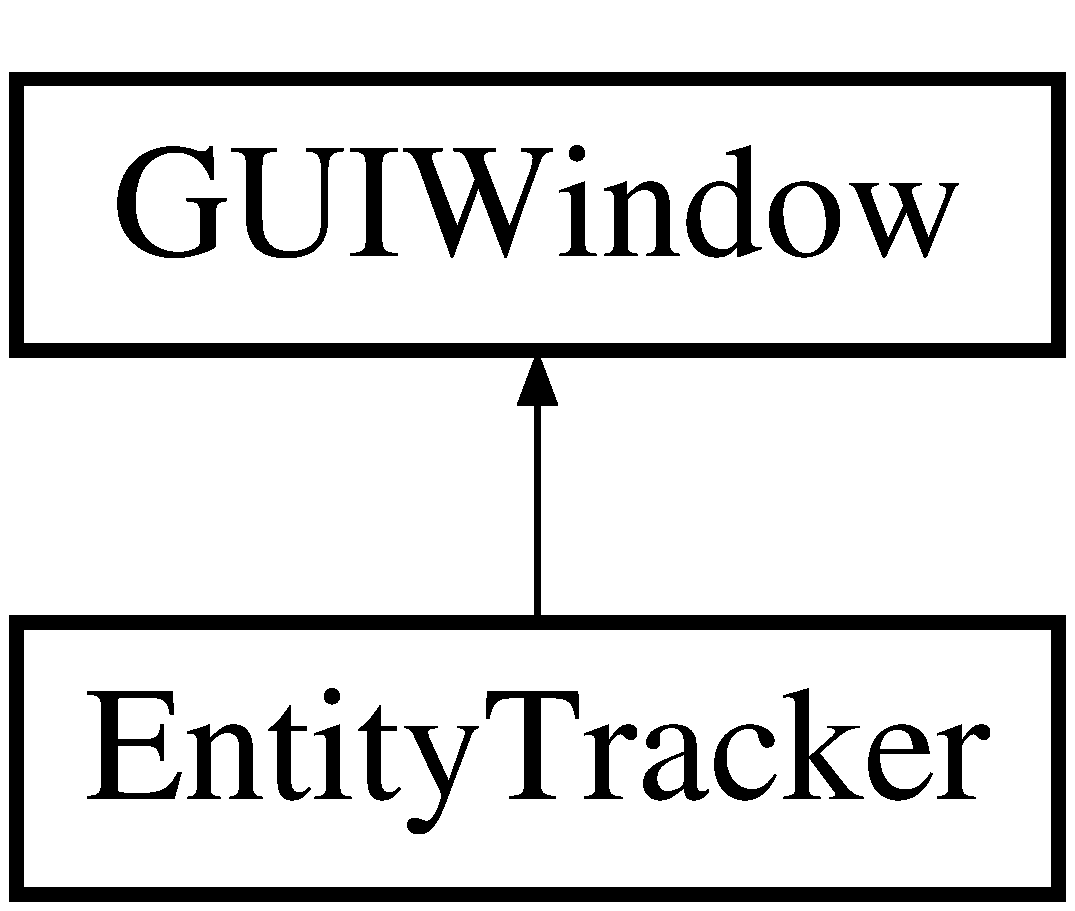
\includegraphics[height=2.000000cm]{class_entity_tracker}
\end{center}
\end{figure}
\subsection*{Public Member Functions}
\begin{DoxyCompactItemize}
\item 
\hyperlink{class_entity_tracker_af562bdb32acbf38e49d146414aefcae7}{Entity\+Tracker} ()
\begin{DoxyCompactList}\small\item\em Constructor. \end{DoxyCompactList}\item 
\hyperlink{class_entity_tracker_a1325c2319379220142156dbb567d45ba}{$\sim$\+Entity\+Tracker} ()=default
\begin{DoxyCompactList}\small\item\em Destructor. \end{DoxyCompactList}\item 
void \hyperlink{class_entity_tracker_abff80cf0f55c307745c5f88f219099a1}{set\+\_\+tracked\+\_\+entity} (tdt\+::uint, \hyperlink{class_entity_system}{Entity\+System} \&)
\begin{DoxyCompactList}\small\item\em Sets the new tracked entity and loads it\textquotesingle{}s data. \end{DoxyCompactList}\item 
tdt\+::uint \hyperlink{class_entity_tracker_ab51ce2487826c578c1b99dbbeae622dc}{get\+\_\+tracked\+\_\+entity} () const 
\begin{DoxyCompactList}\small\item\em Returns the ID of the currently tracked entity. \end{DoxyCompactList}\item 
void \hyperlink{class_entity_tracker_a71f7a58fe7988b4f94fe272a5022f088}{update\+\_\+tracking} (const std\+::string \&, const std\+::string \&)
\begin{DoxyCompactList}\small\item\em Updates a single stat of the entity tracker. \end{DoxyCompactList}\item 
void \hyperlink{class_entity_tracker_a7acaffc973bc0f3de2a1429de72cf825}{clear} ()
\begin{DoxyCompactList}\small\item\em Clears the entity tracker\textquotesingle{}s window, that is sets all values to 0/0 and the id to U\+N\+K\+N\+O\+WN. \end{DoxyCompactList}\item 
void \hyperlink{class_entity_tracker_a562f4a8cfb73794b5e5e21e368057488}{init\+\_\+upgrade\+\_\+butt} (\hyperlink{class_entity_system}{Entity\+System} $\ast$)
\begin{DoxyCompactList}\small\item\em Adds a callback to the U\+P\+G\+R\+A\+DE button that upgrades an entity. \end{DoxyCompactList}\item 
void \hyperlink{class_entity_tracker_a70821e196f3fe0910bf72e6fa664a505}{show\+\_\+upgrade\+\_\+butt} (bool)
\begin{DoxyCompactList}\small\item\em Sets the visibility status of the U\+P\+G\+R\+A\+DE button. \end{DoxyCompactList}\end{DoxyCompactItemize}
\subsection*{Protected Member Functions}
\begin{DoxyCompactItemize}
\item 
void \hyperlink{class_entity_tracker_a4a1051b7efd0414225bd6b19b24bf5b1}{init\+\_\+} () override
\begin{DoxyCompactList}\small\item\em Initializes the window and sets all event subscribers. \end{DoxyCompactList}\end{DoxyCompactItemize}
\subsection*{Private Attributes}
\begin{DoxyCompactItemize}
\item 
tdt\+::uint \hyperlink{class_entity_tracker_a1ef585f0b346bffb880cbbaaa34f1f47}{curr\+\_\+tracked\+\_\+entity\+\_\+}
\begin{DoxyCompactList}\small\item\em ID of the currently tracked entity. \end{DoxyCompactList}\item 
\hyperlink{class_entity_system}{Entity\+System} $\ast$ \hyperlink{class_entity_tracker_ab7988f819653ef5a97df6f28170609d3}{entities\+\_\+}
\begin{DoxyCompactList}\small\item\em Used for upgrading. \end{DoxyCompactList}\end{DoxyCompactItemize}
\subsection*{Additional Inherited Members}


\subsection{Detailed Description}
A window that monitors the stats of the currently selected entity and allows for it\textquotesingle{}s upgrading once it has enough experience. 

Definition at line 11 of file Entity\+Tracker.\+hpp.



\subsection{Constructor \& Destructor Documentation}
\index{Entity\+Tracker@{Entity\+Tracker}!Entity\+Tracker@{Entity\+Tracker}}
\index{Entity\+Tracker@{Entity\+Tracker}!Entity\+Tracker@{Entity\+Tracker}}
\subsubsection[{\texorpdfstring{Entity\+Tracker()}{EntityTracker()}}]{\setlength{\rightskip}{0pt plus 5cm}Entity\+Tracker\+::\+Entity\+Tracker (
\begin{DoxyParamCaption}
{}
\end{DoxyParamCaption}
)}\hypertarget{class_entity_tracker_af562bdb32acbf38e49d146414aefcae7}{}\label{class_entity_tracker_af562bdb32acbf38e49d146414aefcae7}


Constructor. 



Definition at line 7 of file Entity\+Tracker.\+cpp.

\index{Entity\+Tracker@{Entity\+Tracker}!````~Entity\+Tracker@{$\sim$\+Entity\+Tracker}}
\index{````~Entity\+Tracker@{$\sim$\+Entity\+Tracker}!Entity\+Tracker@{Entity\+Tracker}}
\subsubsection[{\texorpdfstring{$\sim$\+Entity\+Tracker()=default}{~EntityTracker()=default}}]{\setlength{\rightskip}{0pt plus 5cm}Entity\+Tracker\+::$\sim$\+Entity\+Tracker (
\begin{DoxyParamCaption}
{}
\end{DoxyParamCaption}
)\hspace{0.3cm}{\ttfamily [default]}}\hypertarget{class_entity_tracker_a1325c2319379220142156dbb567d45ba}{}\label{class_entity_tracker_a1325c2319379220142156dbb567d45ba}


Destructor. 



\subsection{Member Function Documentation}
\index{Entity\+Tracker@{Entity\+Tracker}!clear@{clear}}
\index{clear@{clear}!Entity\+Tracker@{Entity\+Tracker}}
\subsubsection[{\texorpdfstring{clear()}{clear()}}]{\setlength{\rightskip}{0pt plus 5cm}void Entity\+Tracker\+::clear (
\begin{DoxyParamCaption}
{}
\end{DoxyParamCaption}
)}\hypertarget{class_entity_tracker_a7acaffc973bc0f3de2a1429de72cf825}{}\label{class_entity_tracker_a7acaffc973bc0f3de2a1429de72cf825}


Clears the entity tracker\textquotesingle{}s window, that is sets all values to 0/0 and the id to U\+N\+K\+N\+O\+WN. 



Definition at line 70 of file Entity\+Tracker.\+cpp.

\index{Entity\+Tracker@{Entity\+Tracker}!get\+\_\+tracked\+\_\+entity@{get\+\_\+tracked\+\_\+entity}}
\index{get\+\_\+tracked\+\_\+entity@{get\+\_\+tracked\+\_\+entity}!Entity\+Tracker@{Entity\+Tracker}}
\subsubsection[{\texorpdfstring{get\+\_\+tracked\+\_\+entity() const }{get_tracked_entity() const }}]{\setlength{\rightskip}{0pt plus 5cm}tdt\+::uint Entity\+Tracker\+::get\+\_\+tracked\+\_\+entity (
\begin{DoxyParamCaption}
{}
\end{DoxyParamCaption}
) const}\hypertarget{class_entity_tracker_ab51ce2487826c578c1b99dbbeae622dc}{}\label{class_entity_tracker_ab51ce2487826c578c1b99dbbeae622dc}


Returns the ID of the currently tracked entity. 



Definition at line 59 of file Entity\+Tracker.\+cpp.

\index{Entity\+Tracker@{Entity\+Tracker}!init\+\_\+@{init\+\_\+}}
\index{init\+\_\+@{init\+\_\+}!Entity\+Tracker@{Entity\+Tracker}}
\subsubsection[{\texorpdfstring{init\+\_\+() override}{init_() override}}]{\setlength{\rightskip}{0pt plus 5cm}void Entity\+Tracker\+::init\+\_\+ (
\begin{DoxyParamCaption}
{}
\end{DoxyParamCaption}
)\hspace{0.3cm}{\ttfamily [override]}, {\ttfamily [protected]}, {\ttfamily [virtual]}}\hypertarget{class_entity_tracker_a4a1051b7efd0414225bd6b19b24bf5b1}{}\label{class_entity_tracker_a4a1051b7efd0414225bd6b19b24bf5b1}


Initializes the window and sets all event subscribers. 



Implements \hyperlink{class_g_u_i_window_a2a7c011363f401a57a26cc7c7652bdfd}{G\+U\+I\+Window}.



Definition at line 138 of file Entity\+Tracker.\+cpp.

\index{Entity\+Tracker@{Entity\+Tracker}!init\+\_\+upgrade\+\_\+butt@{init\+\_\+upgrade\+\_\+butt}}
\index{init\+\_\+upgrade\+\_\+butt@{init\+\_\+upgrade\+\_\+butt}!Entity\+Tracker@{Entity\+Tracker}}
\subsubsection[{\texorpdfstring{init\+\_\+upgrade\+\_\+butt(\+Entity\+System $\ast$)}{init_upgrade_butt(EntitySystem *)}}]{\setlength{\rightskip}{0pt plus 5cm}void Entity\+Tracker\+::init\+\_\+upgrade\+\_\+butt (
\begin{DoxyParamCaption}
\item[{{\bf Entity\+System} $\ast$}]{ents}
\end{DoxyParamCaption}
)}\hypertarget{class_entity_tracker_a562f4a8cfb73794b5e5e21e368057488}{}\label{class_entity_tracker_a562f4a8cfb73794b5e5e21e368057488}


Adds a callback to the U\+P\+G\+R\+A\+DE button that upgrades an entity. 


\begin{DoxyParams}{Parameters}
{\em Entity} & system containing entities that will be upgraded by this button. \\
\hline
\end{DoxyParams}


Definition at line 87 of file Entity\+Tracker.\+cpp.

\index{Entity\+Tracker@{Entity\+Tracker}!set\+\_\+tracked\+\_\+entity@{set\+\_\+tracked\+\_\+entity}}
\index{set\+\_\+tracked\+\_\+entity@{set\+\_\+tracked\+\_\+entity}!Entity\+Tracker@{Entity\+Tracker}}
\subsubsection[{\texorpdfstring{set\+\_\+tracked\+\_\+entity(tdt\+::uint, Entity\+System \&)}{set_tracked_entity(tdt::uint, EntitySystem &)}}]{\setlength{\rightskip}{0pt plus 5cm}void Entity\+Tracker\+::set\+\_\+tracked\+\_\+entity (
\begin{DoxyParamCaption}
\item[{tdt\+::uint}]{id, }
\item[{{\bf Entity\+System} \&}]{ents}
\end{DoxyParamCaption}
)}\hypertarget{class_entity_tracker_abff80cf0f55c307745c5f88f219099a1}{}\label{class_entity_tracker_abff80cf0f55c307745c5f88f219099a1}


Sets the new tracked entity and loads it\textquotesingle{}s data. 


\begin{DoxyParams}{Parameters}
{\em ID} & of the entity. \\
\hline
{\em \hyperlink{class_entity_system}{Entity\+System}} & that contains the entity. \\
\hline
\end{DoxyParams}


Definition at line 11 of file Entity\+Tracker.\+cpp.

\index{Entity\+Tracker@{Entity\+Tracker}!show\+\_\+upgrade\+\_\+butt@{show\+\_\+upgrade\+\_\+butt}}
\index{show\+\_\+upgrade\+\_\+butt@{show\+\_\+upgrade\+\_\+butt}!Entity\+Tracker@{Entity\+Tracker}}
\subsubsection[{\texorpdfstring{show\+\_\+upgrade\+\_\+butt(bool)}{show_upgrade_butt(bool)}}]{\setlength{\rightskip}{0pt plus 5cm}void Entity\+Tracker\+::show\+\_\+upgrade\+\_\+butt (
\begin{DoxyParamCaption}
\item[{bool}]{val}
\end{DoxyParamCaption}
)}\hypertarget{class_entity_tracker_a70821e196f3fe0910bf72e6fa664a505}{}\label{class_entity_tracker_a70821e196f3fe0910bf72e6fa664a505}


Sets the visibility status of the U\+P\+G\+R\+A\+DE button. 


\begin{DoxyParams}{Parameters}
{\em True} & for visible, false for invisible. \\
\hline
\end{DoxyParams}


Definition at line 133 of file Entity\+Tracker.\+cpp.

\index{Entity\+Tracker@{Entity\+Tracker}!update\+\_\+tracking@{update\+\_\+tracking}}
\index{update\+\_\+tracking@{update\+\_\+tracking}!Entity\+Tracker@{Entity\+Tracker}}
\subsubsection[{\texorpdfstring{update\+\_\+tracking(const std\+::string \&, const std\+::string \&)}{update_tracking(const std::string &, const std::string &)}}]{\setlength{\rightskip}{0pt plus 5cm}void Entity\+Tracker\+::update\+\_\+tracking (
\begin{DoxyParamCaption}
\item[{const std\+::string \&}]{label, }
\item[{const std\+::string \&}]{value}
\end{DoxyParamCaption}
)}\hypertarget{class_entity_tracker_a71f7a58fe7988b4f94fe272a5022f088}{}\label{class_entity_tracker_a71f7a58fe7988b4f94fe272a5022f088}


Updates a single stat of the entity tracker. 


\begin{DoxyParams}{Parameters}
{\em Name} & of the stat label (e.\+g. \char`\"{}\+H\+P\+\_\+\+L\+A\+B\+E\+L\char`\"{}, \char`\"{}\+G\+O\+L\+D\+\_\+\+L\+A\+B\+E\+L\char`\"{} etc). \\
\hline
{\em String} & with the new value. \\
\hline
\end{DoxyParams}
\begin{DoxyNote}{Note}
The value should have the form \char`\"{}\mbox{[}\+C\+U\+R\+R\+E\+N\+T\+\_\+\+V\+A\+L\+U\+E\mbox{]}/\mbox{[}\+M\+A\+X\+\_\+\+V\+A\+L\+U\+E\mbox{]}\char`\"{}. 
\end{DoxyNote}


Definition at line 64 of file Entity\+Tracker.\+cpp.



\subsection{Member Data Documentation}
\index{Entity\+Tracker@{Entity\+Tracker}!curr\+\_\+tracked\+\_\+entity\+\_\+@{curr\+\_\+tracked\+\_\+entity\+\_\+}}
\index{curr\+\_\+tracked\+\_\+entity\+\_\+@{curr\+\_\+tracked\+\_\+entity\+\_\+}!Entity\+Tracker@{Entity\+Tracker}}
\subsubsection[{\texorpdfstring{curr\+\_\+tracked\+\_\+entity\+\_\+}{curr_tracked_entity_}}]{\setlength{\rightskip}{0pt plus 5cm}tdt\+::uint Entity\+Tracker\+::curr\+\_\+tracked\+\_\+entity\+\_\+\hspace{0.3cm}{\ttfamily [private]}}\hypertarget{class_entity_tracker_a1ef585f0b346bffb880cbbaaa34f1f47}{}\label{class_entity_tracker_a1ef585f0b346bffb880cbbaaa34f1f47}


ID of the currently tracked entity. 



Definition at line 72 of file Entity\+Tracker.\+hpp.

\index{Entity\+Tracker@{Entity\+Tracker}!entities\+\_\+@{entities\+\_\+}}
\index{entities\+\_\+@{entities\+\_\+}!Entity\+Tracker@{Entity\+Tracker}}
\subsubsection[{\texorpdfstring{entities\+\_\+}{entities_}}]{\setlength{\rightskip}{0pt plus 5cm}{\bf Entity\+System}$\ast$ Entity\+Tracker\+::entities\+\_\+\hspace{0.3cm}{\ttfamily [private]}}\hypertarget{class_entity_tracker_ab7988f819653ef5a97df6f28170609d3}{}\label{class_entity_tracker_ab7988f819653ef5a97df6f28170609d3}


Used for upgrading. 



Definition at line 77 of file Entity\+Tracker.\+hpp.



The documentation for this class was generated from the following files\+:\begin{DoxyCompactItemize}
\item 
gui/Entity\+Tracker.\+hpp\item 
gui/Entity\+Tracker.\+cpp\end{DoxyCompactItemize}

\hypertarget{struct_event_component}{}\section{Event\+Component Struct Reference}
\label{struct_event_component}\index{Event\+Component@{Event\+Component}}


Represents events that happen in the game, like gold seams dropping gold, curing an entity of poisoning or triggers from traps etc.  




{\ttfamily \#include $<$Components.\+hpp$>$}

\subsection*{Public Member Functions}
\begin{DoxyCompactItemize}
\item 
{\bfseries Event\+Component} (E\+V\+E\+N\+T\+\_\+\+T\+Y\+PE ev=E\+V\+E\+N\+T\+\_\+\+T\+Y\+P\+E\+::\+N\+O\+NE, tdt\+::uint t=Component\+::\+N\+O\+\_\+\+E\+N\+T\+I\+TY, tdt\+::real r=0.f, bool a=true)\hypertarget{struct_event_component_a2aa1deb7ea3815614b05e54da4843a68}{}\label{struct_event_component_a2aa1deb7ea3815614b05e54da4843a68}

\item 
{\bfseries Event\+Component} (const \hyperlink{struct_event_component}{Event\+Component} \&)=default\hypertarget{struct_event_component_a384ff98804daad15afcd85f34e1abd66}{}\label{struct_event_component_a384ff98804daad15afcd85f34e1abd66}

\item 
{\bfseries Event\+Component} (\hyperlink{struct_event_component}{Event\+Component} \&\&)=default\hypertarget{struct_event_component_aa1cc574920ccaa3a62ec781cb8d0d650}{}\label{struct_event_component_aa1cc574920ccaa3a62ec781cb8d0d650}

\item 
\hyperlink{struct_event_component}{Event\+Component} \& {\bfseries operator=} (const \hyperlink{struct_event_component}{Event\+Component} \&)=default\hypertarget{struct_event_component_a3dcc4aab5c42862071d81023168ce832}{}\label{struct_event_component_a3dcc4aab5c42862071d81023168ce832}

\item 
\hyperlink{struct_event_component}{Event\+Component} \& {\bfseries operator=} (\hyperlink{struct_event_component}{Event\+Component} \&\&)=default\hypertarget{struct_event_component_aca718a5d3cefcad57ad321a8e98b12f4}{}\label{struct_event_component_aca718a5d3cefcad57ad321a8e98b12f4}

\end{DoxyCompactItemize}
\subsection*{Public Attributes}
\begin{DoxyCompactItemize}
\item 
E\+V\+E\+N\+T\+\_\+\+T\+Y\+PE {\bfseries event\+\_\+type}\hypertarget{struct_event_component_a258be4826d7efeb3360970b789021c1a}{}\label{struct_event_component_a258be4826d7efeb3360970b789021c1a}

\item 
tdt\+::uint {\bfseries target}\hypertarget{struct_event_component_a1b12eccc9e2bf6132c28a1ba82195a0e}{}\label{struct_event_component_a1b12eccc9e2bf6132c28a1ba82195a0e}

\item 
tdt\+::uint {\bfseries handler}\hypertarget{struct_event_component_a898fb8e2a56106c3eb9fc6bcf314fa16}{}\label{struct_event_component_a898fb8e2a56106c3eb9fc6bcf314fa16}

\item 
tdt\+::real {\bfseries radius}\hypertarget{struct_event_component_a72794d817ae4bd09be962fcb6f4e27e5}{}\label{struct_event_component_a72794d817ae4bd09be962fcb6f4e27e5}

\item 
bool {\bfseries active}\hypertarget{struct_event_component_ae06cba5bf30d9135ae435d0d69f338c3}{}\label{struct_event_component_ae06cba5bf30d9135ae435d0d69f338c3}

\end{DoxyCompactItemize}
\subsection*{Static Public Attributes}
\begin{DoxyCompactItemize}
\item 
static constexpr int {\bfseries type} = 6\hypertarget{struct_event_component_a4f1f827d5a5e38ee791850ffb8460d67}{}\label{struct_event_component_a4f1f827d5a5e38ee791850ffb8460d67}

\end{DoxyCompactItemize}


\subsection{Detailed Description}
Represents events that happen in the game, like gold seams dropping gold, curing an entity of poisoning or triggers from traps etc. 

Definition at line 183 of file Components.\+hpp.



The documentation for this struct was generated from the following file\+:\begin{DoxyCompactItemize}
\item 
Components.\+hpp\end{DoxyCompactItemize}

\hypertarget{struct_event_handler_component}{}\section{Event\+Handler\+Component Struct Reference}
\label{struct_event_handler_component}\index{Event\+Handler\+Component@{Event\+Handler\+Component}}


Allows to cherry pink when it comes to event handling and handle only certain events.  




{\ttfamily \#include $<$Components.\+hpp$>$}

\subsection*{Public Member Functions}
\begin{DoxyCompactItemize}
\item 
{\bfseries Event\+Handler\+Component} (std\+::string \&\&h=\char`\"{}E\+R\+R\+OR\char`\"{})\hypertarget{struct_event_handler_component_af25948d03abfc06f4715abfcd7ec804e}{}\label{struct_event_handler_component_af25948d03abfc06f4715abfcd7ec804e}

\item 
{\bfseries Event\+Handler\+Component} (const \hyperlink{struct_event_handler_component}{Event\+Handler\+Component} \&)=default\hypertarget{struct_event_handler_component_a88f196bdb6a7f2eea224b4d996f543da}{}\label{struct_event_handler_component_a88f196bdb6a7f2eea224b4d996f543da}

\item 
{\bfseries Event\+Handler\+Component} (\hyperlink{struct_event_handler_component}{Event\+Handler\+Component} \&\&)=default\hypertarget{struct_event_handler_component_ad4fa66de6ade475b42b8d666ebf5aa88}{}\label{struct_event_handler_component_ad4fa66de6ade475b42b8d666ebf5aa88}

\item 
\hyperlink{struct_event_handler_component}{Event\+Handler\+Component} \& {\bfseries operator=} (const \hyperlink{struct_event_handler_component}{Event\+Handler\+Component} \&)=default\hypertarget{struct_event_handler_component_a9545cb998a258abb593d0059a62d4a15}{}\label{struct_event_handler_component_a9545cb998a258abb593d0059a62d4a15}

\item 
\hyperlink{struct_event_handler_component}{Event\+Handler\+Component} \& {\bfseries operator=} (\hyperlink{struct_event_handler_component}{Event\+Handler\+Component} \&\&)=default\hypertarget{struct_event_handler_component_a3bd8413f84d5d4a465df5f3d232739a5}{}\label{struct_event_handler_component_a3bd8413f84d5d4a465df5f3d232739a5}

\end{DoxyCompactItemize}
\subsection*{Public Attributes}
\begin{DoxyCompactItemize}
\item 
std\+::string {\bfseries handler}\hypertarget{struct_event_handler_component_a168441f76d9101998be42bde4b5d5acf}{}\label{struct_event_handler_component_a168441f76d9101998be42bde4b5d5acf}

\item 
std\+::bitset$<$(int) E\+V\+E\+N\+T\+\_\+\+T\+Y\+P\+E\+::\+C\+O\+U\+NT $>$ {\bfseries possible\+\_\+events}\hypertarget{struct_event_handler_component_a2dff7cf5e12774036bd149c73bf591e6}{}\label{struct_event_handler_component_a2dff7cf5e12774036bd149c73bf591e6}

\end{DoxyCompactItemize}
\subsection*{Static Public Attributes}
\begin{DoxyCompactItemize}
\item 
static constexpr int {\bfseries type} = 19\hypertarget{struct_event_handler_component_a6b626d9951bf3e8359baea3fdec67d33}{}\label{struct_event_handler_component_a6b626d9951bf3e8359baea3fdec67d33}

\end{DoxyCompactItemize}


\subsection{Detailed Description}
Allows to cherry pink when it comes to event handling and handle only certain events. 

(Also, only entities with this component will react to events.) 

Definition at line 487 of file Components.\+hpp.



The documentation for this struct was generated from the following file\+:\begin{DoxyCompactItemize}
\item 
Components.\+hpp\end{DoxyCompactItemize}

\hypertarget{class_event_system}{}\section{Event\+System Class Reference}
\label{class_event_system}\index{Event\+System@{Event\+System}}
Inheritance diagram for Event\+System\+:\begin{figure}[H]
\begin{center}
\leavevmode
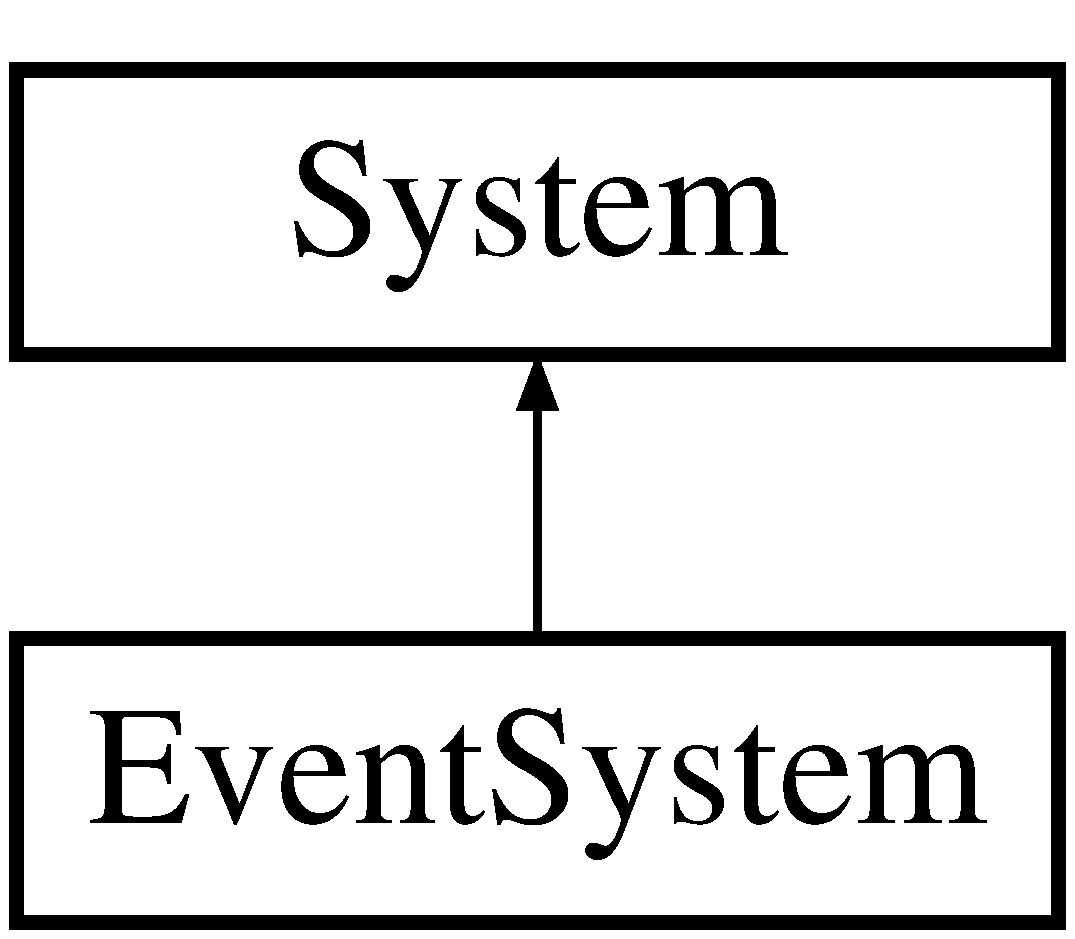
\includegraphics[height=2.000000cm]{class_event_system}
\end{center}
\end{figure}
\subsection*{Public Member Functions}
\begin{DoxyCompactItemize}
\item 
\hyperlink{class_event_system_ae91be44668c9249f29574330794877a6}{Event\+System} (\hyperlink{class_entity_system}{Entity\+System} \&)
\begin{DoxyCompactList}\small\item\em Constructor. \end{DoxyCompactList}\item 
\hyperlink{class_event_system_aaaa3ccbd5dfadfb47d49fd33a2fbc952}{$\sim$\+Event\+System} ()=default
\begin{DoxyCompactList}\small\item\em Destructor. \end{DoxyCompactList}\item 
void \hyperlink{class_event_system_a1410963080a61fdbafc406100dc17d8d}{update} (tdt\+::real) override
\begin{DoxyCompactList}\small\item\em Checks for handlers of all active events and if needed, handles them. \end{DoxyCompactList}\item 
void \hyperlink{class_event_system_a1659caf05f63eaedd1513186574f4292}{set\+\_\+update\+\_\+period} (tdt\+::real)
\begin{DoxyCompactList}\small\item\em Sets the time it takes before an update is performed (in seconds). \end{DoxyCompactList}\item 
tdt\+::real \hyperlink{class_event_system_a1eef89ae00d5f8653c7efe6abeaa40b0}{get\+\_\+update\+\_\+period} () const 
\begin{DoxyCompactList}\small\item\em Returns the time it takes before an update is performed (in seconds). \end{DoxyCompactList}\item 
void \hyperlink{class_event_system_a52087f3b87b190e9cc98cd70b5cbd02d}{set\+\_\+update\+\_\+time\+\_\+multiplier} (tdt\+::real)
\begin{DoxyCompactList}\small\item\em Sets the value by which the frame time is multiplied before it\textquotesingle{}s added to the update timer. \end{DoxyCompactList}\item 
tdt\+::real \hyperlink{class_event_system_ac988bff372a77468dac5fa9b5d9c99ff}{get\+\_\+update\+\_\+time\+\_\+multiplier} () const 
\begin{DoxyCompactList}\small\item\em Returns the value by which the frame time is multiplied before it\textquotesingle{}s added to the update timer. \end{DoxyCompactList}\end{DoxyCompactItemize}
\subsection*{Private Member Functions}
\begin{DoxyCompactItemize}
\item 
bool \hyperlink{class_event_system_aab07d98ea555a11e8cbc6b340371c6ef}{handle\+\_\+event\+\_\+} (tdt\+::uint, tdt\+::uint)
\begin{DoxyCompactList}\small\item\em Handles a given event by a given entity that can handle it, returns true if the event will be destroyed after this call (single handler event), false if the event persist (multi handler event). \end{DoxyCompactList}\end{DoxyCompactItemize}
\subsection*{Private Attributes}
\begin{DoxyCompactItemize}
\item 
\hyperlink{class_entity_system}{Entity\+System} \& \hyperlink{class_event_system_ae68ff7a957934b312a0fa66f52d364c0}{entities\+\_\+}
\begin{DoxyCompactList}\small\item\em Entity system that has entities this system will manage. \end{DoxyCompactList}\item 
tdt\+::real \hyperlink{class_event_system_ae2c07675de523ca6157d766f83447d19}{update\+\_\+period\+\_\+}
\begin{DoxyCompactList}\small\item\em Allow for less frequent updates, since per frame updates are quite unnecessary and resource wasting. \end{DoxyCompactList}\item 
tdt\+::real {\bfseries curr\+\_\+update\+\_\+time\+\_\+}\hypertarget{class_event_system_a122c5df0161e22b46184d6e324d5eb4e}{}\label{class_event_system_a122c5df0161e22b46184d6e324d5eb4e}

\item 
tdt\+::real \hyperlink{class_event_system_a28113a32ef8e7f3a415251b815ac7d0f}{update\+\_\+time\+\_\+multiplier\+\_\+}
\begin{DoxyCompactList}\small\item\em Allows to speed up/slow down the update timer. \end{DoxyCompactList}\end{DoxyCompactItemize}


\subsection{Detailed Description}


Definition at line 7 of file Event\+System.\+hpp.



\subsection{Constructor \& Destructor Documentation}
\index{Event\+System@{Event\+System}!Event\+System@{Event\+System}}
\index{Event\+System@{Event\+System}!Event\+System@{Event\+System}}
\subsubsection[{\texorpdfstring{Event\+System(\+Entity\+System \&)}{EventSystem(EntitySystem &)}}]{\setlength{\rightskip}{0pt plus 5cm}Event\+System\+::\+Event\+System (
\begin{DoxyParamCaption}
\item[{{\bf Entity\+System} \&}]{ents}
\end{DoxyParamCaption}
)}\hypertarget{class_event_system_ae91be44668c9249f29574330794877a6}{}\label{class_event_system_ae91be44668c9249f29574330794877a6}


Constructor. 


\begin{DoxyParams}{Parameters}
{\em Entity} & system that has entities this system will manage. \\
\hline
\end{DoxyParams}


Definition at line 6 of file Event\+System.\+cpp.

\index{Event\+System@{Event\+System}!````~Event\+System@{$\sim$\+Event\+System}}
\index{````~Event\+System@{$\sim$\+Event\+System}!Event\+System@{Event\+System}}
\subsubsection[{\texorpdfstring{$\sim$\+Event\+System()=default}{~EventSystem()=default}}]{\setlength{\rightskip}{0pt plus 5cm}Event\+System\+::$\sim$\+Event\+System (
\begin{DoxyParamCaption}
{}
\end{DoxyParamCaption}
)\hspace{0.3cm}{\ttfamily [default]}}\hypertarget{class_event_system_aaaa3ccbd5dfadfb47d49fd33a2fbc952}{}\label{class_event_system_aaaa3ccbd5dfadfb47d49fd33a2fbc952}


Destructor. 



\subsection{Member Function Documentation}
\index{Event\+System@{Event\+System}!get\+\_\+update\+\_\+period@{get\+\_\+update\+\_\+period}}
\index{get\+\_\+update\+\_\+period@{get\+\_\+update\+\_\+period}!Event\+System@{Event\+System}}
\subsubsection[{\texorpdfstring{get\+\_\+update\+\_\+period() const }{get_update_period() const }}]{\setlength{\rightskip}{0pt plus 5cm}tdt\+::real Event\+System\+::get\+\_\+update\+\_\+period (
\begin{DoxyParamCaption}
{}
\end{DoxyParamCaption}
) const}\hypertarget{class_event_system_a1eef89ae00d5f8653c7efe6abeaa40b0}{}\label{class_event_system_a1eef89ae00d5f8653c7efe6abeaa40b0}


Returns the time it takes before an update is performed (in seconds). 



Definition at line 63 of file Event\+System.\+cpp.

\index{Event\+System@{Event\+System}!get\+\_\+update\+\_\+time\+\_\+multiplier@{get\+\_\+update\+\_\+time\+\_\+multiplier}}
\index{get\+\_\+update\+\_\+time\+\_\+multiplier@{get\+\_\+update\+\_\+time\+\_\+multiplier}!Event\+System@{Event\+System}}
\subsubsection[{\texorpdfstring{get\+\_\+update\+\_\+time\+\_\+multiplier() const }{get_update_time_multiplier() const }}]{\setlength{\rightskip}{0pt plus 5cm}tdt\+::real Event\+System\+::get\+\_\+update\+\_\+time\+\_\+multiplier (
\begin{DoxyParamCaption}
{}
\end{DoxyParamCaption}
) const}\hypertarget{class_event_system_ac988bff372a77468dac5fa9b5d9c99ff}{}\label{class_event_system_ac988bff372a77468dac5fa9b5d9c99ff}


Returns the value by which the frame time is multiplied before it\textquotesingle{}s added to the update timer. 



Definition at line 73 of file Event\+System.\+cpp.

\index{Event\+System@{Event\+System}!handle\+\_\+event\+\_\+@{handle\+\_\+event\+\_\+}}
\index{handle\+\_\+event\+\_\+@{handle\+\_\+event\+\_\+}!Event\+System@{Event\+System}}
\subsubsection[{\texorpdfstring{handle\+\_\+event\+\_\+(tdt\+::uint, tdt\+::uint)}{handle_event_(tdt::uint, tdt::uint)}}]{\setlength{\rightskip}{0pt plus 5cm}bool Event\+System\+::handle\+\_\+event\+\_\+ (
\begin{DoxyParamCaption}
\item[{tdt\+::uint}]{handler, }
\item[{tdt\+::uint}]{evt}
\end{DoxyParamCaption}
)\hspace{0.3cm}{\ttfamily [private]}}\hypertarget{class_event_system_aab07d98ea555a11e8cbc6b340371c6ef}{}\label{class_event_system_aab07d98ea555a11e8cbc6b340371c6ef}


Handles a given event by a given entity that can handle it, returns true if the event will be destroyed after this call (single handler event), false if the event persist (multi handler event). 


\begin{DoxyParams}{Parameters}
{\em ID} & of the handler. \\
\hline
{\em ID} & of the event. \\
\hline
\end{DoxyParams}


Definition at line 78 of file Event\+System.\+cpp.

\index{Event\+System@{Event\+System}!set\+\_\+update\+\_\+period@{set\+\_\+update\+\_\+period}}
\index{set\+\_\+update\+\_\+period@{set\+\_\+update\+\_\+period}!Event\+System@{Event\+System}}
\subsubsection[{\texorpdfstring{set\+\_\+update\+\_\+period(tdt\+::real)}{set_update_period(tdt::real)}}]{\setlength{\rightskip}{0pt plus 5cm}void Event\+System\+::set\+\_\+update\+\_\+period (
\begin{DoxyParamCaption}
\item[{tdt\+::real}]{val}
\end{DoxyParamCaption}
)}\hypertarget{class_event_system_a1659caf05f63eaedd1513186574f4292}{}\label{class_event_system_a1659caf05f63eaedd1513186574f4292}


Sets the time it takes before an update is performed (in seconds). 


\begin{DoxyParams}{Parameters}
{\em The} & new update time period. \\
\hline
\end{DoxyParams}


Definition at line 58 of file Event\+System.\+cpp.

\index{Event\+System@{Event\+System}!set\+\_\+update\+\_\+time\+\_\+multiplier@{set\+\_\+update\+\_\+time\+\_\+multiplier}}
\index{set\+\_\+update\+\_\+time\+\_\+multiplier@{set\+\_\+update\+\_\+time\+\_\+multiplier}!Event\+System@{Event\+System}}
\subsubsection[{\texorpdfstring{set\+\_\+update\+\_\+time\+\_\+multiplier(tdt\+::real)}{set_update_time_multiplier(tdt::real)}}]{\setlength{\rightskip}{0pt plus 5cm}void Event\+System\+::set\+\_\+update\+\_\+time\+\_\+multiplier (
\begin{DoxyParamCaption}
\item[{tdt\+::real}]{val}
\end{DoxyParamCaption}
)}\hypertarget{class_event_system_a52087f3b87b190e9cc98cd70b5cbd02d}{}\label{class_event_system_a52087f3b87b190e9cc98cd70b5cbd02d}


Sets the value by which the frame time is multiplied before it\textquotesingle{}s added to the update timer. 


\begin{DoxyParams}{Parameters}
{\em The} & new multiplier value. \\
\hline
\end{DoxyParams}


Definition at line 68 of file Event\+System.\+cpp.

\index{Event\+System@{Event\+System}!update@{update}}
\index{update@{update}!Event\+System@{Event\+System}}
\subsubsection[{\texorpdfstring{update(tdt\+::real) override}{update(tdt::real) override}}]{\setlength{\rightskip}{0pt plus 5cm}void Event\+System\+::update (
\begin{DoxyParamCaption}
\item[{tdt\+::real}]{delta}
\end{DoxyParamCaption}
)\hspace{0.3cm}{\ttfamily [override]}, {\ttfamily [virtual]}}\hypertarget{class_event_system_a1410963080a61fdbafc406100dc17d8d}{}\label{class_event_system_a1410963080a61fdbafc406100dc17d8d}


Checks for handlers of all active events and if needed, handles them. 


\begin{DoxyParams}{Parameters}
{\em Time} & since last frame. \\
\hline
\end{DoxyParams}


Implements \hyperlink{class_system_a6d54c9bd38eb43d620a1451cb0925472}{System}.



Definition at line 11 of file Event\+System.\+cpp.



\subsection{Member Data Documentation}
\index{Event\+System@{Event\+System}!entities\+\_\+@{entities\+\_\+}}
\index{entities\+\_\+@{entities\+\_\+}!Event\+System@{Event\+System}}
\subsubsection[{\texorpdfstring{entities\+\_\+}{entities_}}]{\setlength{\rightskip}{0pt plus 5cm}{\bf Entity\+System}\& Event\+System\+::entities\+\_\+\hspace{0.3cm}{\ttfamily [private]}}\hypertarget{class_event_system_ae68ff7a957934b312a0fa66f52d364c0}{}\label{class_event_system_ae68ff7a957934b312a0fa66f52d364c0}


Entity system that has entities this system will manage. 



Definition at line 67 of file Event\+System.\+hpp.

\index{Event\+System@{Event\+System}!update\+\_\+period\+\_\+@{update\+\_\+period\+\_\+}}
\index{update\+\_\+period\+\_\+@{update\+\_\+period\+\_\+}!Event\+System@{Event\+System}}
\subsubsection[{\texorpdfstring{update\+\_\+period\+\_\+}{update_period_}}]{\setlength{\rightskip}{0pt plus 5cm}tdt\+::real Event\+System\+::update\+\_\+period\+\_\+\hspace{0.3cm}{\ttfamily [private]}}\hypertarget{class_event_system_ae2c07675de523ca6157d766f83447d19}{}\label{class_event_system_ae2c07675de523ca6157d766f83447d19}


Allow for less frequent updates, since per frame updates are quite unnecessary and resource wasting. 



Definition at line 73 of file Event\+System.\+hpp.

\index{Event\+System@{Event\+System}!update\+\_\+time\+\_\+multiplier\+\_\+@{update\+\_\+time\+\_\+multiplier\+\_\+}}
\index{update\+\_\+time\+\_\+multiplier\+\_\+@{update\+\_\+time\+\_\+multiplier\+\_\+}!Event\+System@{Event\+System}}
\subsubsection[{\texorpdfstring{update\+\_\+time\+\_\+multiplier\+\_\+}{update_time_multiplier_}}]{\setlength{\rightskip}{0pt plus 5cm}tdt\+::real Event\+System\+::update\+\_\+time\+\_\+multiplier\+\_\+\hspace{0.3cm}{\ttfamily [private]}}\hypertarget{class_event_system_a28113a32ef8e7f3a415251b815ac7d0f}{}\label{class_event_system_a28113a32ef8e7f3a415251b815ac7d0f}


Allows to speed up/slow down the update timer. 



Definition at line 78 of file Event\+System.\+hpp.



The documentation for this class was generated from the following files\+:\begin{DoxyCompactItemize}
\item 
systems/Event\+System.\+hpp\item 
systems/Event\+System.\+cpp\end{DoxyCompactItemize}

\hypertarget{classlpp_1_1_exception}{}\section{lpp\+:\+:Exception Class Reference}
\label{classlpp_1_1_exception}\index{lpp\+::\+Exception@{lpp\+::\+Exception}}


\hyperlink{classlpp_1_1_exception}{Exception} class used to throw exception from the \hyperlink{classlpp_1_1_script}{Script} class.  




{\ttfamily \#include $<$Lpp\+Script.\+hpp$>$}

\subsection*{Public Member Functions}
\begin{DoxyCompactItemize}
\item 
\hyperlink{classlpp_1_1_exception_a1ff116cf88d7b05c3584877648ca82ab}{Exception} (const std\+::string \&msg=\char`\"{}NO M\+SG\char`\"{}, Script\+::state L=nullptr)
\begin{DoxyCompactList}\small\item\em Constructor. \end{DoxyCompactList}\item 
const char $\ast$ \hyperlink{classlpp_1_1_exception_ac20670138a33c7785532349e9bb6504b}{what} () const 
\begin{DoxyCompactList}\small\item\em Returns the message of this exception. \end{DoxyCompactList}\item 
const char $\ast$ \hyperlink{classlpp_1_1_exception_a3a02de1c4c93591ccfc6baeb71298d79}{what\+\_\+lua} () const 
\begin{DoxyCompactList}\small\item\em Returns the Lua error message if possible. \end{DoxyCompactList}\item 
bool \hyperlink{classlpp_1_1_exception_a0286545c71695a14ec1d30242e54afbd}{has\+\_\+lua\+\_\+state} () const 
\begin{DoxyCompactList}\small\item\em Returns true if a Lua state is captured by this exception. \end{DoxyCompactList}\end{DoxyCompactItemize}
\subsection*{Private Attributes}
\begin{DoxyCompactItemize}
\item 
std\+::string \hyperlink{classlpp_1_1_exception_a6e7e0df55bd44c48f72ed1d3289a54e3}{msg\+\_\+}
\begin{DoxyCompactList}\small\item\em Message the exception was called with. \end{DoxyCompactList}\item 
Script\+::state \hyperlink{classlpp_1_1_exception_a0384a7b078e9ad4ded648a100955a013}{L\+\_\+}
\begin{DoxyCompactList}\small\item\em Pointer to the Lua state, used for stack manipulation (like lua error retrieval). \end{DoxyCompactList}\end{DoxyCompactItemize}


\subsection{Detailed Description}
\hyperlink{classlpp_1_1_exception}{Exception} class used to throw exception from the \hyperlink{classlpp_1_1_script}{Script} class. 

Definition at line 266 of file Lpp\+Script.\+hpp.



\subsection{Constructor \& Destructor Documentation}
\index{lpp\+::\+Exception@{lpp\+::\+Exception}!Exception@{Exception}}
\index{Exception@{Exception}!lpp\+::\+Exception@{lpp\+::\+Exception}}
\subsubsection[{\texorpdfstring{Exception(const std\+::string \&msg=""N\+O M\+SG"", Script\+::state L=nullptr)}{Exception(const std::string &msg="NO MSG", Script::state L=nullptr)}}]{\setlength{\rightskip}{0pt plus 5cm}lpp\+::\+Exception\+::\+Exception (
\begin{DoxyParamCaption}
\item[{const std\+::string \&}]{msg = {\ttfamily \char`\"{}NO~MSG\char`\"{}}, }
\item[{Script\+::state}]{L = {\ttfamily nullptr}}
\end{DoxyParamCaption}
)\hspace{0.3cm}{\ttfamily [inline]}}\hypertarget{classlpp_1_1_exception_a1ff116cf88d7b05c3584877648ca82ab}{}\label{classlpp_1_1_exception_a1ff116cf88d7b05c3584877648ca82ab}


Constructor. 


\begin{DoxyParams}{Parameters}
{\em Message} & of the exception. \\
\hline
\end{DoxyParams}


Definition at line 273 of file Lpp\+Script.\+hpp.



\subsection{Member Function Documentation}
\index{lpp\+::\+Exception@{lpp\+::\+Exception}!has\+\_\+lua\+\_\+state@{has\+\_\+lua\+\_\+state}}
\index{has\+\_\+lua\+\_\+state@{has\+\_\+lua\+\_\+state}!lpp\+::\+Exception@{lpp\+::\+Exception}}
\subsubsection[{\texorpdfstring{has\+\_\+lua\+\_\+state() const }{has_lua_state() const }}]{\setlength{\rightskip}{0pt plus 5cm}bool lpp\+::\+Exception\+::has\+\_\+lua\+\_\+state (
\begin{DoxyParamCaption}
{}
\end{DoxyParamCaption}
) const}\hypertarget{classlpp_1_1_exception_a0286545c71695a14ec1d30242e54afbd}{}\label{classlpp_1_1_exception_a0286545c71695a14ec1d30242e54afbd}


Returns true if a Lua state is captured by this exception. 



Definition at line 128 of file Lpp\+Script.\+cpp.

\index{lpp\+::\+Exception@{lpp\+::\+Exception}!what@{what}}
\index{what@{what}!lpp\+::\+Exception@{lpp\+::\+Exception}}
\subsubsection[{\texorpdfstring{what() const }{what() const }}]{\setlength{\rightskip}{0pt plus 5cm}const char $\ast$ lpp\+::\+Exception\+::what (
\begin{DoxyParamCaption}
{}
\end{DoxyParamCaption}
) const}\hypertarget{classlpp_1_1_exception_ac20670138a33c7785532349e9bb6504b}{}\label{classlpp_1_1_exception_ac20670138a33c7785532349e9bb6504b}


Returns the message of this exception. 

\hyperlink{classlpp_1_1_exception}{lpp\+::\+Exception} definitions\+: 

Definition at line 114 of file Lpp\+Script.\+cpp.

\index{lpp\+::\+Exception@{lpp\+::\+Exception}!what\+\_\+lua@{what\+\_\+lua}}
\index{what\+\_\+lua@{what\+\_\+lua}!lpp\+::\+Exception@{lpp\+::\+Exception}}
\subsubsection[{\texorpdfstring{what\+\_\+lua() const }{what_lua() const }}]{\setlength{\rightskip}{0pt plus 5cm}const char $\ast$ lpp\+::\+Exception\+::what\+\_\+lua (
\begin{DoxyParamCaption}
{}
\end{DoxyParamCaption}
) const}\hypertarget{classlpp_1_1_exception_a3a02de1c4c93591ccfc6baeb71298d79}{}\label{classlpp_1_1_exception_a3a02de1c4c93591ccfc6baeb71298d79}


Returns the Lua error message if possible. 



Definition at line 119 of file Lpp\+Script.\+cpp.



\subsection{Member Data Documentation}
\index{lpp\+::\+Exception@{lpp\+::\+Exception}!L\+\_\+@{L\+\_\+}}
\index{L\+\_\+@{L\+\_\+}!lpp\+::\+Exception@{lpp\+::\+Exception}}
\subsubsection[{\texorpdfstring{L\+\_\+}{L_}}]{\setlength{\rightskip}{0pt plus 5cm}Script\+::state lpp\+::\+Exception\+::\+L\+\_\+\hspace{0.3cm}{\ttfamily [private]}}\hypertarget{classlpp_1_1_exception_a0384a7b078e9ad4ded648a100955a013}{}\label{classlpp_1_1_exception_a0384a7b078e9ad4ded648a100955a013}


Pointer to the Lua state, used for stack manipulation (like lua error retrieval). 



Definition at line 301 of file Lpp\+Script.\+hpp.

\index{lpp\+::\+Exception@{lpp\+::\+Exception}!msg\+\_\+@{msg\+\_\+}}
\index{msg\+\_\+@{msg\+\_\+}!lpp\+::\+Exception@{lpp\+::\+Exception}}
\subsubsection[{\texorpdfstring{msg\+\_\+}{msg_}}]{\setlength{\rightskip}{0pt plus 5cm}std\+::string lpp\+::\+Exception\+::msg\+\_\+\hspace{0.3cm}{\ttfamily [private]}}\hypertarget{classlpp_1_1_exception_a6e7e0df55bd44c48f72ed1d3289a54e3}{}\label{classlpp_1_1_exception_a6e7e0df55bd44c48f72ed1d3289a54e3}


Message the exception was called with. 



Definition at line 296 of file Lpp\+Script.\+hpp.



The documentation for this class was generated from the following files\+:\begin{DoxyCompactItemize}
\item 
lppscript/Lpp\+Script.\+hpp\item 
lppscript/Lpp\+Script.\+cpp\end{DoxyCompactItemize}

\hypertarget{struct_experience_value_component}{}\section{Experience\+Value\+Component Struct Reference}
\label{struct_experience_value_component}\index{Experience\+Value\+Component@{Experience\+Value\+Component}}


The amount of experience the entity yields when killed.  




{\ttfamily \#include $<$Components.\+hpp$>$}

\subsection*{Public Member Functions}
\begin{DoxyCompactItemize}
\item 
{\bfseries Experience\+Value\+Component} (tdt\+::uint v=0)\hypertarget{struct_experience_value_component_a6c771930a164bd7208fc305acc229807}{}\label{struct_experience_value_component_a6c771930a164bd7208fc305acc229807}

\item 
{\bfseries Experience\+Value\+Component} (const \hyperlink{struct_experience_value_component}{Experience\+Value\+Component} \&)=default\hypertarget{struct_experience_value_component_a21c33f33e9fc9c8279b0c5f48ca83ccf}{}\label{struct_experience_value_component_a21c33f33e9fc9c8279b0c5f48ca83ccf}

\item 
{\bfseries Experience\+Value\+Component} (\hyperlink{struct_experience_value_component}{Experience\+Value\+Component} \&\&)=default\hypertarget{struct_experience_value_component_a33518c5195dc24e347836312aefc8fab}{}\label{struct_experience_value_component_a33518c5195dc24e347836312aefc8fab}

\item 
\hyperlink{struct_experience_value_component}{Experience\+Value\+Component} \& {\bfseries operator=} (const \hyperlink{struct_experience_value_component}{Experience\+Value\+Component} \&)=default\hypertarget{struct_experience_value_component_ad055d663d9924442969f5bdf5f95d1c8}{}\label{struct_experience_value_component_ad055d663d9924442969f5bdf5f95d1c8}

\item 
\hyperlink{struct_experience_value_component}{Experience\+Value\+Component} \& {\bfseries operator=} (\hyperlink{struct_experience_value_component}{Experience\+Value\+Component} \&\&)=default\hypertarget{struct_experience_value_component_acc124046259f20bc40b94ce2bc5e60f8}{}\label{struct_experience_value_component_acc124046259f20bc40b94ce2bc5e60f8}

\end{DoxyCompactItemize}
\subsection*{Public Attributes}
\begin{DoxyCompactItemize}
\item 
tdt\+::uint {\bfseries value}\hypertarget{struct_experience_value_component_af23c393293e39fabc99cfee417bb038c}{}\label{struct_experience_value_component_af23c393293e39fabc99cfee417bb038c}

\end{DoxyCompactItemize}
\subsection*{Static Public Attributes}
\begin{DoxyCompactItemize}
\item 
static constexpr int {\bfseries type} = 35\hypertarget{struct_experience_value_component_aec9243dc7a28d3e133900d2367a00818}{}\label{struct_experience_value_component_aec9243dc7a28d3e133900d2367a00818}

\end{DoxyCompactItemize}


\subsection{Detailed Description}
The amount of experience the entity yields when killed. 

Definition at line 822 of file Components.\+hpp.



The documentation for this struct was generated from the following file\+:\begin{DoxyCompactItemize}
\item 
Components.\+hpp\end{DoxyCompactItemize}

\hypertarget{struct_explosion_component}{}\section{Explosion\+Component Struct Reference}
\label{struct_explosion_component}\index{Explosion\+Component@{Explosion\+Component}}


\hyperlink{struct_component}{Component} used to create the visual effect of an explosion, the damage should be done in the explosion\textquotesingle{}s constructor so that it\textquotesingle{}s not applied on each frame.  




{\ttfamily \#include $<$Components.\+hpp$>$}

\subsection*{Public Member Functions}
\begin{DoxyCompactItemize}
\item 
{\bfseries Explosion\+Component} (tdt\+::real d=0.f, tdt\+::real rad=0.f)\hypertarget{struct_explosion_component_ae83e0ea9dfc9580a5443ca8cc0836522}{}\label{struct_explosion_component_ae83e0ea9dfc9580a5443ca8cc0836522}

\item 
{\bfseries Explosion\+Component} (const \hyperlink{struct_explosion_component}{Explosion\+Component} \&)=default\hypertarget{struct_explosion_component_a359fb260499fab4e45b9e47e114b4e2c}{}\label{struct_explosion_component_a359fb260499fab4e45b9e47e114b4e2c}

\item 
{\bfseries Explosion\+Component} (\hyperlink{struct_explosion_component}{Explosion\+Component} \&\&)=default\hypertarget{struct_explosion_component_ac3edad4b0610493d4d8c667c096a6266}{}\label{struct_explosion_component_ac3edad4b0610493d4d8c667c096a6266}

\item 
\hyperlink{struct_explosion_component}{Explosion\+Component} \& {\bfseries operator=} (const \hyperlink{struct_explosion_component}{Explosion\+Component} \&)=default\hypertarget{struct_explosion_component_ae55cb8d9a7f3db1c1c7f0750de17a9b4}{}\label{struct_explosion_component_ae55cb8d9a7f3db1c1c7f0750de17a9b4}

\item 
\hyperlink{struct_explosion_component}{Explosion\+Component} \& {\bfseries operator=} (\hyperlink{struct_explosion_component}{Explosion\+Component} \&\&)=default\hypertarget{struct_explosion_component_a27a2332fb4795cb1babf0f6244517b1b}{}\label{struct_explosion_component_a27a2332fb4795cb1babf0f6244517b1b}

\end{DoxyCompactItemize}
\subsection*{Public Attributes}
\begin{DoxyCompactItemize}
\item 
tdt\+::real {\bfseries delta}\hypertarget{struct_explosion_component_a528fb7dd7384ec53530fcc3911cc4108}{}\label{struct_explosion_component_a528fb7dd7384ec53530fcc3911cc4108}

\item 
tdt\+::real {\bfseries max\+\_\+radius}\hypertarget{struct_explosion_component_a036937d4523e0ca25434048c3f248ffb}{}\label{struct_explosion_component_a036937d4523e0ca25434048c3f248ffb}

\item 
tdt\+::real {\bfseries curr\+\_\+radius}\hypertarget{struct_explosion_component_aee72886e30f94bbe495708aba9050c51}{}\label{struct_explosion_component_aee72886e30f94bbe495708aba9050c51}

\end{DoxyCompactItemize}
\subsection*{Static Public Attributes}
\begin{DoxyCompactItemize}
\item 
static constexpr int {\bfseries type} = 32\hypertarget{struct_explosion_component_afd2057c1401a1c850f4ee6de18b2f043}{}\label{struct_explosion_component_afd2057c1401a1c850f4ee6de18b2f043}

\end{DoxyCompactItemize}


\subsection{Detailed Description}
\hyperlink{struct_component}{Component} used to create the visual effect of an explosion, the damage should be done in the explosion\textquotesingle{}s constructor so that it\textquotesingle{}s not applied on each frame. 

Definition at line 761 of file Components.\+hpp.



The documentation for this struct was generated from the following file\+:\begin{DoxyCompactItemize}
\item 
Components.\+hpp\end{DoxyCompactItemize}

\hypertarget{struct_faction_component}{}\section{Faction\+Component Struct Reference}
\label{struct_faction_component}\index{Faction\+Component@{Faction\+Component}}


Represents the faction an entity that has this component if a member of.  




{\ttfamily \#include $<$Components.\+hpp$>$}

\subsection*{Public Member Functions}
\begin{DoxyCompactItemize}
\item 
{\bfseries Faction\+Component} (F\+A\+C\+T\+I\+ON f=F\+A\+C\+T\+I\+O\+N\+::\+N\+E\+U\+T\+R\+AL)\hypertarget{struct_faction_component_ada93ef76a2110fb92cbf2d2971cad139}{}\label{struct_faction_component_ada93ef76a2110fb92cbf2d2971cad139}

\item 
{\bfseries Faction\+Component} (const \hyperlink{struct_faction_component}{Faction\+Component} \&)=default\hypertarget{struct_faction_component_a0416d9a5435c81dc2df095b145dd49f4}{}\label{struct_faction_component_a0416d9a5435c81dc2df095b145dd49f4}

\item 
{\bfseries Faction\+Component} (\hyperlink{struct_faction_component}{Faction\+Component} \&\&)=default\hypertarget{struct_faction_component_a5307de75b0571b6f6d2bf1f71399f111}{}\label{struct_faction_component_a5307de75b0571b6f6d2bf1f71399f111}

\item 
\hyperlink{struct_faction_component}{Faction\+Component} \& {\bfseries operator=} (const \hyperlink{struct_faction_component}{Faction\+Component} \&)=default\hypertarget{struct_faction_component_a5aa9e9593b87e724bcf93381a825a39c}{}\label{struct_faction_component_a5aa9e9593b87e724bcf93381a825a39c}

\item 
\hyperlink{struct_faction_component}{Faction\+Component} \& {\bfseries operator=} (\hyperlink{struct_faction_component}{Faction\+Component} \&\&)=default\hypertarget{struct_faction_component_aa707ae4a3f7c95140d21e290649152bd}{}\label{struct_faction_component_aa707ae4a3f7c95140d21e290649152bd}

\end{DoxyCompactItemize}
\subsection*{Public Attributes}
\begin{DoxyCompactItemize}
\item 
F\+A\+C\+T\+I\+ON {\bfseries faction}\hypertarget{struct_faction_component_aad10499e3145f032068dc94120b6564a}{}\label{struct_faction_component_aad10499e3145f032068dc94120b6564a}

\end{DoxyCompactItemize}
\subsection*{Static Public Attributes}
\begin{DoxyCompactItemize}
\item 
static constexpr int {\bfseries type} = 22\hypertarget{struct_faction_component_a39a377f8a913b350da8de13ea335726d}{}\label{struct_faction_component_a39a377f8a913b350da8de13ea335726d}

\end{DoxyCompactItemize}


\subsection{Detailed Description}
Represents the faction an entity that has this component if a member of. 

Definition at line 549 of file Components.\+hpp.



The documentation for this struct was generated from the following file\+:\begin{DoxyCompactItemize}
\item 
Components.\+hpp\end{DoxyCompactItemize}

\hypertarget{structutil_1_1path__type_1_1_f_i_r_s_t___p_a_t_h}{}\section{util\+:\+:path\+\_\+type\+:\+:F\+I\+R\+S\+T\+\_\+\+P\+A\+TH Struct Reference}
\label{structutil_1_1path__type_1_1_f_i_r_s_t___p_a_t_h}\index{util\+::path\+\_\+type\+::\+F\+I\+R\+S\+T\+\_\+\+P\+A\+TH@{util\+::path\+\_\+type\+::\+F\+I\+R\+S\+T\+\_\+\+P\+A\+TH}}


Finds the first path by accepting the first path found.  




{\ttfamily \#include $<$Pathfinding\+Algorithms.\+hpp$>$}

\subsection*{Static Public Member Functions}
\begin{DoxyCompactItemize}
\item 
static bool {\bfseries return\+\_\+path} ()\hypertarget{structutil_1_1path__type_1_1_f_i_r_s_t___p_a_t_h_a89ad468d39aff4c8b18212a5f57cd90b}{}\label{structutil_1_1path__type_1_1_f_i_r_s_t___p_a_t_h_a89ad468d39aff4c8b18212a5f57cd90b}

\end{DoxyCompactItemize}


\subsection{Detailed Description}
Finds the first path by accepting the first path found. 

Definition at line 154 of file Pathfinding\+Algorithms.\+hpp.



The documentation for this struct was generated from the following file\+:\begin{DoxyCompactItemize}
\item 
tools/Pathfinding\+Algorithms.\+hpp\end{DoxyCompactItemize}

\hypertarget{structutil_1_1effect_1_1_f_r_e_e_z_e___e_f_f_e_c_t}{}\section{util\+:\+:effect\+:\+:F\+R\+E\+E\+Z\+E\+\_\+\+E\+F\+F\+E\+CT Struct Reference}
\label{structutil_1_1effect_1_1_f_r_e_e_z_e___e_f_f_e_c_t}\index{util\+::effect\+::\+F\+R\+E\+E\+Z\+E\+\_\+\+E\+F\+F\+E\+CT@{util\+::effect\+::\+F\+R\+E\+E\+Z\+E\+\_\+\+E\+F\+F\+E\+CT}}


Freezes a given entity in place for a given time period.  




{\ttfamily \#include $<$Effects.\+hpp$>$}

\subsection*{Public Member Functions}
\begin{DoxyCompactItemize}
\item 
\hyperlink{structutil_1_1effect_1_1_f_r_e_e_z_e___e_f_f_e_c_t_aca7fba095c1647b74d818ff73696c8b9}{F\+R\+E\+E\+Z\+E\+\_\+\+E\+F\+F\+E\+CT} (\hyperlink{class_entity_system}{Entity\+System} \&, tdt\+::real)
\begin{DoxyCompactList}\small\item\em Constructor. \end{DoxyCompactList}\item 
\hyperlink{structutil_1_1effect_1_1_f_r_e_e_z_e___e_f_f_e_c_t_a1434b6ee911b6586e8466fa0aa6fc0e0}{$\sim$\+F\+R\+E\+E\+Z\+E\+\_\+\+E\+F\+F\+E\+CT} ()=default
\begin{DoxyCompactList}\small\item\em Destructor. \end{DoxyCompactList}\item 
void \hyperlink{structutil_1_1effect_1_1_f_r_e_e_z_e___e_f_f_e_c_t_aa5bc5da43f7d9e15b84bc9b482524b16}{operator()} (tdt\+::uint)
\begin{DoxyCompactList}\small\item\em Freezes a given entity in place. \end{DoxyCompactList}\end{DoxyCompactItemize}
\subsection*{Private Attributes}
\begin{DoxyCompactItemize}
\item 
\hyperlink{class_entity_system}{Entity\+System} \& \hyperlink{structutil_1_1effect_1_1_f_r_e_e_z_e___e_f_f_e_c_t_a1ee6ce1353f02563e70a7c03cebebf4c}{entities\+\_\+}
\begin{DoxyCompactList}\small\item\em Entity system containing the entities this effect will be called on. \end{DoxyCompactList}\item 
tdt\+::real \hyperlink{structutil_1_1effect_1_1_f_r_e_e_z_e___e_f_f_e_c_t_a075e8ad726e06baafced711a2209b55c}{time\+\_\+}
\begin{DoxyCompactList}\small\item\em The duration of the freeze. \end{DoxyCompactList}\end{DoxyCompactItemize}


\subsection{Detailed Description}
Freezes a given entity in place for a given time period. 

(This effect stops movement but not any other action.) 

Definition at line 133 of file Effects.\+hpp.



\subsection{Constructor \& Destructor Documentation}
\index{util\+::effect\+::\+F\+R\+E\+E\+Z\+E\+\_\+\+E\+F\+F\+E\+CT@{util\+::effect\+::\+F\+R\+E\+E\+Z\+E\+\_\+\+E\+F\+F\+E\+CT}!F\+R\+E\+E\+Z\+E\+\_\+\+E\+F\+F\+E\+CT@{F\+R\+E\+E\+Z\+E\+\_\+\+E\+F\+F\+E\+CT}}
\index{F\+R\+E\+E\+Z\+E\+\_\+\+E\+F\+F\+E\+CT@{F\+R\+E\+E\+Z\+E\+\_\+\+E\+F\+F\+E\+CT}!util\+::effect\+::\+F\+R\+E\+E\+Z\+E\+\_\+\+E\+F\+F\+E\+CT@{util\+::effect\+::\+F\+R\+E\+E\+Z\+E\+\_\+\+E\+F\+F\+E\+CT}}
\subsubsection[{\texorpdfstring{F\+R\+E\+E\+Z\+E\+\_\+\+E\+F\+F\+E\+C\+T(\+Entity\+System \&, tdt\+::real)}{FREEZE_EFFECT(EntitySystem &, tdt::real)}}]{\setlength{\rightskip}{0pt plus 5cm}util\+::effect\+::\+F\+R\+E\+E\+Z\+E\+\_\+\+E\+F\+F\+E\+C\+T\+::\+F\+R\+E\+E\+Z\+E\+\_\+\+E\+F\+F\+E\+CT (
\begin{DoxyParamCaption}
\item[{{\bf Entity\+System} \&}]{ents, }
\item[{tdt\+::real}]{time}
\end{DoxyParamCaption}
)}\hypertarget{structutil_1_1effect_1_1_f_r_e_e_z_e___e_f_f_e_c_t_aca7fba095c1647b74d818ff73696c8b9}{}\label{structutil_1_1effect_1_1_f_r_e_e_z_e___e_f_f_e_c_t_aca7fba095c1647b74d818ff73696c8b9}


Constructor. 


\begin{DoxyParams}{Parameters}
{\em Entity} & system containing the entities this effect will be called on. \\
\hline
{\em Duration} & of the freeze. \\
\hline
\end{DoxyParams}


Definition at line 58 of file Effects.\+cpp.

\index{util\+::effect\+::\+F\+R\+E\+E\+Z\+E\+\_\+\+E\+F\+F\+E\+CT@{util\+::effect\+::\+F\+R\+E\+E\+Z\+E\+\_\+\+E\+F\+F\+E\+CT}!````~F\+R\+E\+E\+Z\+E\+\_\+\+E\+F\+F\+E\+CT@{$\sim$\+F\+R\+E\+E\+Z\+E\+\_\+\+E\+F\+F\+E\+CT}}
\index{````~F\+R\+E\+E\+Z\+E\+\_\+\+E\+F\+F\+E\+CT@{$\sim$\+F\+R\+E\+E\+Z\+E\+\_\+\+E\+F\+F\+E\+CT}!util\+::effect\+::\+F\+R\+E\+E\+Z\+E\+\_\+\+E\+F\+F\+E\+CT@{util\+::effect\+::\+F\+R\+E\+E\+Z\+E\+\_\+\+E\+F\+F\+E\+CT}}
\subsubsection[{\texorpdfstring{$\sim$\+F\+R\+E\+E\+Z\+E\+\_\+\+E\+F\+F\+E\+C\+T()=default}{~FREEZE_EFFECT()=default}}]{\setlength{\rightskip}{0pt plus 5cm}util\+::effect\+::\+F\+R\+E\+E\+Z\+E\+\_\+\+E\+F\+F\+E\+C\+T\+::$\sim$\+F\+R\+E\+E\+Z\+E\+\_\+\+E\+F\+F\+E\+CT (
\begin{DoxyParamCaption}
{}
\end{DoxyParamCaption}
)\hspace{0.3cm}{\ttfamily [default]}}\hypertarget{structutil_1_1effect_1_1_f_r_e_e_z_e___e_f_f_e_c_t_a1434b6ee911b6586e8466fa0aa6fc0e0}{}\label{structutil_1_1effect_1_1_f_r_e_e_z_e___e_f_f_e_c_t_a1434b6ee911b6586e8466fa0aa6fc0e0}


Destructor. 



\subsection{Member Function Documentation}
\index{util\+::effect\+::\+F\+R\+E\+E\+Z\+E\+\_\+\+E\+F\+F\+E\+CT@{util\+::effect\+::\+F\+R\+E\+E\+Z\+E\+\_\+\+E\+F\+F\+E\+CT}!operator()@{operator()}}
\index{operator()@{operator()}!util\+::effect\+::\+F\+R\+E\+E\+Z\+E\+\_\+\+E\+F\+F\+E\+CT@{util\+::effect\+::\+F\+R\+E\+E\+Z\+E\+\_\+\+E\+F\+F\+E\+CT}}
\subsubsection[{\texorpdfstring{operator()(tdt\+::uint)}{operator()(tdt::uint)}}]{\setlength{\rightskip}{0pt plus 5cm}void util\+::effect\+::\+F\+R\+E\+E\+Z\+E\+\_\+\+E\+F\+F\+E\+C\+T\+::operator() (
\begin{DoxyParamCaption}
\item[{tdt\+::uint}]{id}
\end{DoxyParamCaption}
)}\hypertarget{structutil_1_1effect_1_1_f_r_e_e_z_e___e_f_f_e_c_t_aa5bc5da43f7d9e15b84bc9b482524b16}{}\label{structutil_1_1effect_1_1_f_r_e_e_z_e___e_f_f_e_c_t_aa5bc5da43f7d9e15b84bc9b482524b16}


Freezes a given entity in place. 


\begin{DoxyParams}{Parameters}
{\em ID} & of the entity. \\
\hline
\end{DoxyParams}


Definition at line 62 of file Effects.\+cpp.



\subsection{Member Data Documentation}
\index{util\+::effect\+::\+F\+R\+E\+E\+Z\+E\+\_\+\+E\+F\+F\+E\+CT@{util\+::effect\+::\+F\+R\+E\+E\+Z\+E\+\_\+\+E\+F\+F\+E\+CT}!entities\+\_\+@{entities\+\_\+}}
\index{entities\+\_\+@{entities\+\_\+}!util\+::effect\+::\+F\+R\+E\+E\+Z\+E\+\_\+\+E\+F\+F\+E\+CT@{util\+::effect\+::\+F\+R\+E\+E\+Z\+E\+\_\+\+E\+F\+F\+E\+CT}}
\subsubsection[{\texorpdfstring{entities\+\_\+}{entities_}}]{\setlength{\rightskip}{0pt plus 5cm}{\bf Entity\+System}\& util\+::effect\+::\+F\+R\+E\+E\+Z\+E\+\_\+\+E\+F\+F\+E\+C\+T\+::entities\+\_\+\hspace{0.3cm}{\ttfamily [private]}}\hypertarget{structutil_1_1effect_1_1_f_r_e_e_z_e___e_f_f_e_c_t_a1ee6ce1353f02563e70a7c03cebebf4c}{}\label{structutil_1_1effect_1_1_f_r_e_e_z_e___e_f_f_e_c_t_a1ee6ce1353f02563e70a7c03cebebf4c}


Entity system containing the entities this effect will be called on. 



Definition at line 159 of file Effects.\+hpp.

\index{util\+::effect\+::\+F\+R\+E\+E\+Z\+E\+\_\+\+E\+F\+F\+E\+CT@{util\+::effect\+::\+F\+R\+E\+E\+Z\+E\+\_\+\+E\+F\+F\+E\+CT}!time\+\_\+@{time\+\_\+}}
\index{time\+\_\+@{time\+\_\+}!util\+::effect\+::\+F\+R\+E\+E\+Z\+E\+\_\+\+E\+F\+F\+E\+CT@{util\+::effect\+::\+F\+R\+E\+E\+Z\+E\+\_\+\+E\+F\+F\+E\+CT}}
\subsubsection[{\texorpdfstring{time\+\_\+}{time_}}]{\setlength{\rightskip}{0pt plus 5cm}tdt\+::real util\+::effect\+::\+F\+R\+E\+E\+Z\+E\+\_\+\+E\+F\+F\+E\+C\+T\+::time\+\_\+\hspace{0.3cm}{\ttfamily [private]}}\hypertarget{structutil_1_1effect_1_1_f_r_e_e_z_e___e_f_f_e_c_t_a075e8ad726e06baafced711a2209b55c}{}\label{structutil_1_1effect_1_1_f_r_e_e_z_e___e_f_f_e_c_t_a075e8ad726e06baafced711a2209b55c}


The duration of the freeze. 



Definition at line 164 of file Effects.\+hpp.



The documentation for this struct was generated from the following files\+:\begin{DoxyCompactItemize}
\item 
tools/Effects.\+hpp\item 
tools/Effects.\+cpp\end{DoxyCompactItemize}

\hypertarget{class_game}{}\section{Game Class Reference}
\label{class_game}\index{Game@{Game}}
Inheritance diagram for Game\+:\begin{figure}[H]
\begin{center}
\leavevmode
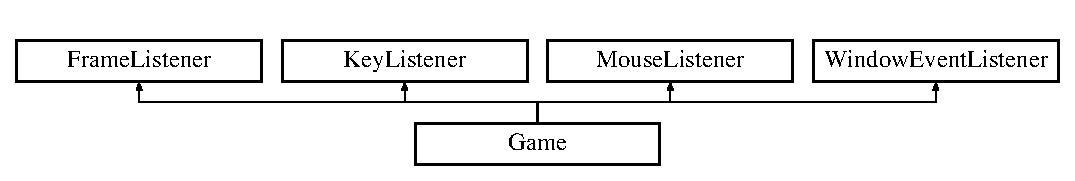
\includegraphics[height=1.985816cm]{class_game}
\end{center}
\end{figure}
\subsection*{Public Member Functions}
\begin{DoxyCompactItemize}
\item 
\hyperlink{class_game_ad59df6562a58a614fda24622d3715b65}{Game} ()
\begin{DoxyCompactList}\small\item\em Constructor. \end{DoxyCompactList}\item 
\hyperlink{class_game_ae3d112ca6e0e55150d2fdbc704474530}{$\sim$\+Game} ()
\begin{DoxyCompactList}\small\item\em Destructor. \end{DoxyCompactList}\item 
void \hyperlink{class_game_a1ab78f5ed0d5ea879157357cf2fb2afa}{run} ()
\begin{DoxyCompactList}\small\item\em Starts the game. \end{DoxyCompactList}\item 
void \hyperlink{class_game_a484567626eb22fe9fc65c51a3914e230}{update} (tdt\+::real)
\begin{DoxyCompactList}\small\item\em Updates the game in one frame. \end{DoxyCompactList}\item 
void \hyperlink{class_game_a5daa13180764435151f08925edd144a3}{set\+\_\+state} (G\+A\+M\+E\+\_\+\+S\+T\+A\+TE)
\begin{DoxyCompactList}\small\item\em Changes the game\textquotesingle{}s state. \end{DoxyCompactList}\item 
void \hyperlink{class_game_af379c92d7e4e03982bcbeb53f4d3edb5}{new\+\_\+game} (tdt\+::uint, tdt\+::uint)
\begin{DoxyCompactList}\small\item\em Creates a new game with the given dimensions. \end{DoxyCompactList}\item 
void \hyperlink{class_game_a57ad62417505d7230bc46b37def4f1d0}{create\+\_\+empty\+\_\+level} (tdt\+::uint, tdt\+::uint)
\begin{DoxyCompactList}\small\item\em Creates an empty level with the given dimensions. \end{DoxyCompactList}\item 
void \hyperlink{class_game_a4faa3b6fdf7446e3e432d3a7cf49e6b2}{reset\+\_\+camera} ()
\begin{DoxyCompactList}\small\item\em Resets the main camera\textquotesingle{}s position and orientation to it\textquotesingle{}s original state. \end{DoxyCompactList}\item 
void \hyperlink{class_game_a64bfdd3eb56fb04275ec65bfa3ae12f6}{reset\+\_\+unlocks} ()
\begin{DoxyCompactList}\small\item\em Restores the unlocks to their initial state. \end{DoxyCompactList}\item 
void \hyperlink{class_game_a20ded9865809df42b8e6d6dd5292351c}{set\+\_\+throne\+\_\+id} (tdt\+::uint)
\begin{DoxyCompactList}\small\item\em Sets the ID of the entity that represents the Dungeon Throne. \end{DoxyCompactList}\item 
tdt\+::uint \hyperlink{class_game_a11e7bc665ccfcd21403f8fad66deb24e}{get\+\_\+throne\+\_\+id} () const 
\begin{DoxyCompactList}\small\item\em Returns the ID of the entity that represents the Dungeon Throne. \end{DoxyCompactList}\end{DoxyCompactItemize}
\subsection*{Protected Member Functions}
\begin{DoxyCompactItemize}
\item 
bool \hyperlink{class_game_a7595cce82f9d32a21ac96663d5927e2b}{frame\+Rendering\+Queued} (const Ogre\+::\+Frame\+Event \&) override
\begin{DoxyCompactList}\small\item\em Called when the previous frame is queued for rendering, used for game updates. \end{DoxyCompactList}\item 
bool \hyperlink{class_game_afa42cb4d67e91e865f0df410a3950c33}{key\+Pressed} (const O\+I\+S\+::\+Key\+Event \&) override
\begin{DoxyCompactList}\small\item\em Called when a key is pressed. \end{DoxyCompactList}\item 
bool \hyperlink{class_game_a30dbe1a49eeef33b8bfdba3275e03b81}{key\+Released} (const O\+I\+S\+::\+Key\+Event \&) override
\begin{DoxyCompactList}\small\item\em Called when a key is released. \end{DoxyCompactList}\item 
bool \hyperlink{class_game_af65edfac010ab689d4f1750de04a3635}{mouse\+Moved} (const O\+I\+S\+::\+Mouse\+Event \&) override
\begin{DoxyCompactList}\small\item\em Called when the mouse is moved. \end{DoxyCompactList}\item 
bool \hyperlink{class_game_a08e8d993e88ef586468a19ad3c45479c}{mouse\+Pressed} (const O\+I\+S\+::\+Mouse\+Event \&, O\+I\+S\+::\+Mouse\+Button\+ID) override
\begin{DoxyCompactList}\small\item\em Called when a mouse button is pressed. \end{DoxyCompactList}\item 
bool \hyperlink{class_game_a32b8ef3a9f1d9103ad4560ca212c2ab1}{mouse\+Released} (const O\+I\+S\+::\+Mouse\+Event \&, O\+I\+S\+::\+Mouse\+Button\+ID) override
\begin{DoxyCompactList}\small\item\em Called when a mouse button is released. \end{DoxyCompactList}\item 
void \hyperlink{class_game_ac04dd2e6cc4b77fa09d234446ff7d1ca}{window\+Resized} (Ogre\+::\+Render\+Window $\ast$rw) override
\begin{DoxyCompactList}\small\item\em Called when the window is resized. \end{DoxyCompactList}\item 
void \hyperlink{class_game_a6d4e1f9eca561e5d10f46e2453df8d9b}{window\+Closed} (Ogre\+::\+Render\+Window $\ast$rw) override
\begin{DoxyCompactList}\small\item\em Called when the window is closed. \end{DoxyCompactList}\end{DoxyCompactItemize}
\subsection*{Private Member Functions}
\begin{DoxyCompactItemize}
\item 
void \hyperlink{class_game_a6c94b1e2b66f522a3ccfe4294d0311d9}{ogre\+\_\+init} ()
\begin{DoxyCompactList}\small\item\em Init methods. \end{DoxyCompactList}\item 
void {\bfseries ois\+\_\+init} ()\hypertarget{class_game_a3541e05c8df317dd0e0a5c6eb1be18cb}{}\label{class_game_a3541e05c8df317dd0e0a5c6eb1be18cb}

\item 
void {\bfseries cegui\+\_\+init} ()\hypertarget{class_game_a0ea174fc98e0557ea5a8719ed1c42fca}{}\label{class_game_a0ea174fc98e0557ea5a8719ed1c42fca}

\item 
C\+E\+G\+U\+I\+::\+Mouse\+Button \hyperlink{class_game_a8a1c953c9c8ca4ef292e5fa6fec4dcb0}{ois\+\_\+to\+\_\+cegui} (O\+I\+S\+::\+Mouse\+Button\+ID)
\begin{DoxyCompactList}\small\item\em Converts an O\+IS key code to C\+E\+G\+UI key code. \end{DoxyCompactList}\item 
void \hyperlink{class_game_a25c49dd9183cb89c0c3e3c34d69389c7}{toggle\+\_\+camera\+\_\+free\+\_\+mode} ()
\begin{DoxyCompactList}\small\item\em Toggles the free camera movement mode. \end{DoxyCompactList}\item 
std\+::pair$<$ bool, Ogre\+::\+Vector3 $>$ \hyperlink{class_game_a215e7330ada9260773a74ad0347dd638}{get\+\_\+mouse\+\_\+click\+\_\+position} (const O\+I\+S\+::\+Mouse\+Event \&) const 
\begin{DoxyCompactList}\small\item\em Returns a pair consisting of the location of the point where the player clicked on the ground plane and a boolean indicating if the click was indeed on the ground plane. \end{DoxyCompactList}\end{DoxyCompactItemize}
\subsection*{Private Attributes}
\begin{DoxyCompactItemize}
\item 
G\+A\+M\+E\+\_\+\+S\+T\+A\+TE \hyperlink{class_game_ab0c5032f689e8e704086a83bf57e3f26}{state\+\_\+}
\begin{DoxyCompactList}\small\item\em Current game state. \end{DoxyCompactList}\item 
std\+::unique\+\_\+ptr$<$ Ogre\+::\+Root $>$ \hyperlink{class_game_ac427345eb3f0b4aa9a6a4a29a195cc61}{root\+\_\+}
\begin{DoxyCompactList}\small\item\em Pointers to Ogre3D objects. \end{DoxyCompactList}\item 
Ogre\+::\+Scene\+Manager $\ast$ {\bfseries scene\+\_\+mgr\+\_\+}\hypertarget{class_game_aea01a069f07ad326a0dd94f1239d06b1}{}\label{class_game_aea01a069f07ad326a0dd94f1239d06b1}

\item 
Ogre\+::\+Render\+Window $\ast$ {\bfseries window\+\_\+}\hypertarget{class_game_a1881d8362923bcf00014d3a22df568fe}{}\label{class_game_a1881d8362923bcf00014d3a22df568fe}

\item 
Ogre\+::\+Viewport $\ast$ {\bfseries main\+\_\+view\+\_\+}\hypertarget{class_game_a31f75ba18f6462b57c8aa9b4d8ec0137}{}\label{class_game_a31f75ba18f6462b57c8aa9b4d8ec0137}

\item 
Ogre\+::\+Light $\ast$ {\bfseries main\+\_\+light\+\_\+}\hypertarget{class_game_a976e47151729dc5e0b4cf60fbdaa7e5e}{}\label{class_game_a976e47151729dc5e0b4cf60fbdaa7e5e}

\item 
O\+I\+S\+::\+Input\+Manager $\ast$ {\bfseries input\+\_\+}\hypertarget{class_game_a7d4c7d5cf1ef4a650c04cc16b0400953}{}\label{class_game_a7d4c7d5cf1ef4a650c04cc16b0400953}

\item 
O\+I\+S\+::\+Keyboard $\ast$ {\bfseries keyboard\+\_\+}\hypertarget{class_game_adcb64e869eada39fe8fb7403311c5411}{}\label{class_game_adcb64e869eada39fe8fb7403311c5411}

\item 
O\+I\+S\+::\+Mouse $\ast$ {\bfseries mouse\+\_\+}\hypertarget{class_game_afa6eb9a23546a694f4bfe175f91ca7d7}{}\label{class_game_afa6eb9a23546a694f4bfe175f91ca7d7}

\item 
std\+::unique\+\_\+ptr$<$ \hyperlink{class_camera}{Camera} $>$ \hyperlink{class_game_a0376227db8220eefaf7f6ac310c091f7}{main\+\_\+cam\+\_\+}
\begin{DoxyCompactList}\small\item\em \hyperlink{class_camera}{Camera} rendering to the window. \end{DoxyCompactList}\item 
std\+::unique\+\_\+ptr$<$ \hyperlink{class_entity_system}{Entity\+System} $>$ \hyperlink{class_game_ab64dd8e6b94e4ea96da9cba633524cdb}{entity\+\_\+system\+\_\+} \{nullptr\}
\begin{DoxyCompactList}\small\item\em Unique pointers to systems (sadly all systems require the \hyperlink{class_entity_system}{Entity\+System}, which requires Ogre\+::\+Scene\+Manager, so the all have to be instantiated after the ogre\+\_\+init method call and thus cannot be references). \end{DoxyCompactList}\item 
std\+::unique\+\_\+ptr$<$ \hyperlink{class_health_system}{Health\+System} $>$ {\bfseries health\+\_\+system\+\_\+} \{nullptr\}\hypertarget{class_game_af74712bd1667aa653794d9faf843c844}{}\label{class_game_af74712bd1667aa653794d9faf843c844}

\item 
std\+::unique\+\_\+ptr$<$ \hyperlink{class_movement_system}{Movement\+System} $>$ {\bfseries movement\+\_\+system\+\_\+} \{nullptr\}\hypertarget{class_game_a67305bc37d65d7dd32e7a523576d9c52}{}\label{class_game_a67305bc37d65d7dd32e7a523576d9c52}

\item 
std\+::unique\+\_\+ptr$<$ \hyperlink{class_a_i_system}{A\+I\+System} $>$ {\bfseries ai\+\_\+system\+\_\+} \{nullptr\}\hypertarget{class_game_ab7a06b3de828f2e6150acf1663e1183a}{}\label{class_game_ab7a06b3de828f2e6150acf1663e1183a}

\item 
std\+::unique\+\_\+ptr$<$ \hyperlink{class_input_system}{Input\+System} $>$ {\bfseries input\+\_\+system\+\_\+} \{nullptr\}\hypertarget{class_game_ab2c619644c9f7e5701aec29258956f50}{}\label{class_game_ab2c619644c9f7e5701aec29258956f50}

\item 
std\+::unique\+\_\+ptr$<$ \hyperlink{class_grid_system}{Grid\+System} $>$ {\bfseries grid\+\_\+system\+\_\+} \{nullptr\}\hypertarget{class_game_ab78af70efdfac02836b368fcf434a750}{}\label{class_game_ab78af70efdfac02836b368fcf434a750}

\item 
std\+::unique\+\_\+ptr$<$ \hyperlink{class_task_system}{Task\+System} $>$ {\bfseries task\+\_\+system\+\_\+} \{nullptr\}\hypertarget{class_game_ace7adb25b62f8b56cd0c004c9d2e4ad8}{}\label{class_game_ace7adb25b62f8b56cd0c004c9d2e4ad8}

\item 
std\+::unique\+\_\+ptr$<$ \hyperlink{class_combat_system}{Combat\+System} $>$ {\bfseries combat\+\_\+system\+\_\+} \{nullptr\}\hypertarget{class_game_ac749b13cf8ad3a0629b5af28d4e81b75}{}\label{class_game_ac749b13cf8ad3a0629b5af28d4e81b75}

\item 
std\+::unique\+\_\+ptr$<$ \hyperlink{class_production_system}{Production\+System} $>$ {\bfseries production\+\_\+system\+\_\+} \{nullptr\}\hypertarget{class_game_a1eee6c4d037835a6fec98e4cbc1b91b0}{}\label{class_game_a1eee6c4d037835a6fec98e4cbc1b91b0}

\item 
std\+::unique\+\_\+ptr$<$ \hyperlink{class_time_system}{Time\+System} $>$ {\bfseries time\+\_\+system\+\_\+} \{nullptr\}\hypertarget{class_game_add56890bc1393af525a2658ff0476221}{}\label{class_game_add56890bc1393af525a2658ff0476221}

\item 
std\+::unique\+\_\+ptr$<$ \hyperlink{class_event_system}{Event\+System} $>$ {\bfseries event\+\_\+system\+\_\+} \{nullptr\}\hypertarget{class_game_a2e8dd50347570cc742aef91e6f065312}{}\label{class_game_a2e8dd50347570cc742aef91e6f065312}

\item 
std\+::unique\+\_\+ptr$<$ \hyperlink{class_graphics_system}{Graphics\+System} $>$ {\bfseries graphics\+\_\+system\+\_\+} \{nullptr\}\hypertarget{class_game_aa1bee90e713de5f7b151fee08bdb9926}{}\label{class_game_aa1bee90e713de5f7b151fee08bdb9926}

\item 
std\+::unique\+\_\+ptr$<$ \hyperlink{class_trigger_system}{Trigger\+System} $>$ {\bfseries trigger\+\_\+system\+\_\+} \{nullptr\}\hypertarget{class_game_a7909364b4dac4fda1ae101dc63d5cef8}{}\label{class_game_a7909364b4dac4fda1ae101dc63d5cef8}

\item 
std\+::unique\+\_\+ptr$<$ \hyperlink{class_mana_spell_system}{Mana\+Spell\+System} $>$ {\bfseries mana\+\_\+spell\+\_\+system\+\_\+} \{nullptr\}\hypertarget{class_game_a8e5ab6f6e518ae3a137594d109906c11}{}\label{class_game_a8e5ab6f6e518ae3a137594d109906c11}

\item 
std\+::unique\+\_\+ptr$<$ \hyperlink{class_wave_system}{Wave\+System} $>$ {\bfseries wave\+\_\+system\+\_\+} \{nullptr\}\hypertarget{class_game_aec046435ac5dd6cda77f7e94fd22d06f}{}\label{class_game_aec046435ac5dd6cda77f7e94fd22d06f}

\item 
std\+::unique\+\_\+ptr$<$ \hyperlink{class_game_serializer}{Game\+Serializer} $>$ \hyperlink{class_game_a27543a5588f79f251f5b4cb64026966f}{game\+\_\+serializer\+\_\+} \{nullptr\}
\begin{DoxyCompactList}\small\item\em Used to save the game. \end{DoxyCompactList}\item 
std\+::vector$<$ \hyperlink{class_system}{System} $\ast$ $>$ \hyperlink{class_game_af594421c81bec3f6284ccdb8d3888080}{systems\+\_\+} \{\}
\begin{DoxyCompactList}\small\item\em Vector of all systems used for updating the game\textquotesingle{}s logic. \end{DoxyCompactList}\item 
C\+E\+G\+U\+I\+::\+Ogre\+Renderer $\ast$ \hyperlink{class_game_a55d453a75a2abc8a0b2ba4ad6265b8c3}{renderer\+\_\+}
\begin{DoxyCompactList}\small\item\em C\+E\+G\+UI renderer. \end{DoxyCompactList}\item 
std\+::unique\+\_\+ptr$<$ \hyperlink{class_entity_placer}{Entity\+Placer} $>$ \hyperlink{class_game_a9ce203f7a53ba536a1d7653f7e74d05f}{placer\+\_\+}
\begin{DoxyCompactList}\small\item\em Allows to spawn entities with the mouse ingame. \end{DoxyCompactList}\item 
std\+::unique\+\_\+ptr$<$ Ogre\+::\+Plane $>$ \hyperlink{class_game_a8e687faa09ca8c2f89279eecbe463916}{ground\+\_\+}
\begin{DoxyCompactList}\small\item\em The game\textquotesingle{}s ground represented by a plane, used for ray intersections. \end{DoxyCompactList}\item 
Ogre\+::\+Entity $\ast$ \hyperlink{class_game_a13668cabb42e440fea0f0a2a2b211984}{ground\+\_\+entity\+\_\+}
\begin{DoxyCompactList}\small\item\em Entity holding the ground plane. \end{DoxyCompactList}\item 
std\+::unique\+\_\+ptr$<$ \hyperlink{class_selection_box}{Selection\+Box} $>$ \hyperlink{class_game_af49a6f70e2392c419e0bbc6157b809a4}{selection\+\_\+box\+\_\+}
\begin{DoxyCompactList}\small\item\em Selection box used to select multiple entities at once. \end{DoxyCompactList}\item 
std\+::unique\+\_\+ptr$<$ \hyperlink{class_entity_creator}{Entity\+Creator} $>$ \hyperlink{class_game_ad5a3e4b03b13386ab6dd759017573821}{entity\+\_\+creator\+\_\+}
\begin{DoxyCompactList}\small\item\em A gui window that allows to place entities selected from a menu. \end{DoxyCompactList}\item 
Ogre\+::\+Vector2 \hyperlink{class_game_abd514cad4e3b88d5ab87e8f2e966fd4a}{mouse\+\_\+position\+\_\+}
\begin{DoxyCompactList}\small\item\em Saved position of the mouse cursor (2D). \end{DoxyCompactList}\item 
std\+::unique\+\_\+ptr$<$ \hyperlink{classlevel__generators_1_1_level_generator}{level\+\_\+generators\+::\+Level\+Generator} $>$ \hyperlink{class_game_a180d400b3d9f3781f31822f9141704b2}{level\+\_\+generator\+\_\+}
\begin{DoxyCompactList}\small\item\em Used to create new levels (that is, to distribute walls and gold deposits). \end{DoxyCompactList}\item 
std\+::unique\+\_\+ptr$<$ \hyperlink{class_spellcaster}{Spellcaster} $>$ \hyperlink{class_game_a16f63fa6189119f189b90129558af639}{spell\+\_\+caster\+\_\+}
\begin{DoxyCompactList}\small\item\em Allows the player to cast spells of different types (positional, targeted etc.). \end{DoxyCompactList}\item 
tdt\+::uint \hyperlink{class_game_add2c7263d03befb832ce112ccf09b3eb}{throne\+\_\+id\+\_\+}
\begin{DoxyCompactList}\small\item\em ID of the entity representing the Dungeon Throne, losing which ends the game. \end{DoxyCompactList}\end{DoxyCompactItemize}
\subsection*{Friends}
\begin{DoxyCompactItemize}
\item 
class {\bfseries Game\+Serializer}\hypertarget{class_game_a6f4a2258d01e962995f3a4743b711864}{}\label{class_game_a6f4a2258d01e962995f3a4743b711864}

\item 
class {\bfseries Lua\+Interface}\hypertarget{class_game_acd4772e3fbf5a45415bf704538df08a4}{}\label{class_game_acd4772e3fbf5a45415bf704538df08a4}

\item 
class {\bfseries G\+UI}\hypertarget{class_game_ac5a3536de371167fdf200e8943f8c2b0}{}\label{class_game_ac5a3536de371167fdf200e8943f8c2b0}

\item 
void {\bfseries action\+::\+Q\+U\+I\+C\+K\+\_\+\+L\+O\+AD} ()\hypertarget{class_game_afcaa4fe027cc52b7f11e80caedfb2f96}{}\label{class_game_afcaa4fe027cc52b7f11e80caedfb2f96}

\item 
void {\bfseries action\+::\+Q\+U\+I\+C\+K\+\_\+\+S\+A\+VE} ()\hypertarget{class_game_ac91f206467cf888fb767b7d7d03b92ba}{}\label{class_game_ac91f206467cf888fb767b7d7d03b92ba}

\item 
void {\bfseries action\+::\+R\+E\+S\+E\+T\+\_\+\+C\+A\+M\+E\+RA} ()\hypertarget{class_game_a94cac4560c54379f3013e5074558f322}{}\label{class_game_a94cac4560c54379f3013e5074558f322}

\end{DoxyCompactItemize}


\subsection{Detailed Description}


Definition at line 40 of file Game.\+hpp.



\subsection{Constructor \& Destructor Documentation}
\index{Game@{Game}!Game@{Game}}
\index{Game@{Game}!Game@{Game}}
\subsubsection[{\texorpdfstring{Game()}{Game()}}]{\setlength{\rightskip}{0pt plus 5cm}Game\+::\+Game (
\begin{DoxyParamCaption}
{}
\end{DoxyParamCaption}
)}\hypertarget{class_game_ad59df6562a58a614fda24622d3715b65}{}\label{class_game_ad59df6562a58a614fda24622d3715b65}


Constructor. 



Definition at line 30 of file Game.\+cpp.

\index{Game@{Game}!````~Game@{$\sim$\+Game}}
\index{````~Game@{$\sim$\+Game}!Game@{Game}}
\subsubsection[{\texorpdfstring{$\sim$\+Game()}{~Game()}}]{\setlength{\rightskip}{0pt plus 5cm}Game\+::$\sim$\+Game (
\begin{DoxyParamCaption}
{}
\end{DoxyParamCaption}
)}\hypertarget{class_game_ae3d112ca6e0e55150d2fdbc704474530}{}\label{class_game_ae3d112ca6e0e55150d2fdbc704474530}


Destructor. 



Definition at line 104 of file Game.\+cpp.



\subsection{Member Function Documentation}
\index{Game@{Game}!create\+\_\+empty\+\_\+level@{create\+\_\+empty\+\_\+level}}
\index{create\+\_\+empty\+\_\+level@{create\+\_\+empty\+\_\+level}!Game@{Game}}
\subsubsection[{\texorpdfstring{create\+\_\+empty\+\_\+level(tdt\+::uint, tdt\+::uint)}{create_empty_level(tdt::uint, tdt::uint)}}]{\setlength{\rightskip}{0pt plus 5cm}void Game\+::create\+\_\+empty\+\_\+level (
\begin{DoxyParamCaption}
\item[{tdt\+::uint}]{width, }
\item[{tdt\+::uint}]{height}
\end{DoxyParamCaption}
)}\hypertarget{class_game_a57ad62417505d7230bc46b37def4f1d0}{}\label{class_game_a57ad62417505d7230bc46b37def4f1d0}


Creates an empty level with the given dimensions. 


\begin{DoxyParams}{Parameters}
{\em Width} & of the level. \\
\hline
{\em Height} & of the level. \\
\hline
\end{DoxyParams}


Definition at line 186 of file Game.\+cpp.

\index{Game@{Game}!frame\+Rendering\+Queued@{frame\+Rendering\+Queued}}
\index{frame\+Rendering\+Queued@{frame\+Rendering\+Queued}!Game@{Game}}
\subsubsection[{\texorpdfstring{frame\+Rendering\+Queued(const Ogre\+::\+Frame\+Event \&) override}{frameRenderingQueued(const Ogre::FrameEvent &) override}}]{\setlength{\rightskip}{0pt plus 5cm}bool Game\+::frame\+Rendering\+Queued (
\begin{DoxyParamCaption}
\item[{const Ogre\+::\+Frame\+Event \&}]{event}
\end{DoxyParamCaption}
)\hspace{0.3cm}{\ttfamily [override]}, {\ttfamily [protected]}}\hypertarget{class_game_a7595cce82f9d32a21ac96663d5927e2b}{}\label{class_game_a7595cce82f9d32a21ac96663d5927e2b}


Called when the previous frame is queued for rendering, used for game updates. 



Definition at line 264 of file Game.\+cpp.

\index{Game@{Game}!get\+\_\+mouse\+\_\+click\+\_\+position@{get\+\_\+mouse\+\_\+click\+\_\+position}}
\index{get\+\_\+mouse\+\_\+click\+\_\+position@{get\+\_\+mouse\+\_\+click\+\_\+position}!Game@{Game}}
\subsubsection[{\texorpdfstring{get\+\_\+mouse\+\_\+click\+\_\+position(const O\+I\+S\+::\+Mouse\+Event \&) const }{get_mouse_click_position(const OIS::MouseEvent &) const }}]{\setlength{\rightskip}{0pt plus 5cm}std\+::pair$<$ bool, Ogre\+::\+Vector3 $>$ Game\+::get\+\_\+mouse\+\_\+click\+\_\+position (
\begin{DoxyParamCaption}
\item[{const O\+I\+S\+::\+Mouse\+Event \&}]{event}
\end{DoxyParamCaption}
) const\hspace{0.3cm}{\ttfamily [private]}}\hypertarget{class_game_a215e7330ada9260773a74ad0347dd638}{}\label{class_game_a215e7330ada9260773a74ad0347dd638}


Returns a pair consisting of the location of the point where the player clicked on the ground plane and a boolean indicating if the click was indeed on the ground plane. 



Definition at line 631 of file Game.\+cpp.

\index{Game@{Game}!get\+\_\+throne\+\_\+id@{get\+\_\+throne\+\_\+id}}
\index{get\+\_\+throne\+\_\+id@{get\+\_\+throne\+\_\+id}!Game@{Game}}
\subsubsection[{\texorpdfstring{get\+\_\+throne\+\_\+id() const }{get_throne_id() const }}]{\setlength{\rightskip}{0pt plus 5cm}tdt\+::uint Game\+::get\+\_\+throne\+\_\+id (
\begin{DoxyParamCaption}
{}
\end{DoxyParamCaption}
) const}\hypertarget{class_game_a11e7bc665ccfcd21403f8fad66deb24e}{}\label{class_game_a11e7bc665ccfcd21403f8fad66deb24e}


Returns the ID of the entity that represents the Dungeon Throne. 



Definition at line 259 of file Game.\+cpp.

\index{Game@{Game}!key\+Pressed@{key\+Pressed}}
\index{key\+Pressed@{key\+Pressed}!Game@{Game}}
\subsubsection[{\texorpdfstring{key\+Pressed(const O\+I\+S\+::\+Key\+Event \&) override}{keyPressed(const OIS::KeyEvent &) override}}]{\setlength{\rightskip}{0pt plus 5cm}bool Game\+::key\+Pressed (
\begin{DoxyParamCaption}
\item[{const O\+I\+S\+::\+Key\+Event \&}]{event}
\end{DoxyParamCaption}
)\hspace{0.3cm}{\ttfamily [override]}, {\ttfamily [protected]}}\hypertarget{class_game_afa42cb4d67e91e865f0df410a3950c33}{}\label{class_game_afa42cb4d67e91e865f0df410a3950c33}


Called when a key is pressed. 



Definition at line 278 of file Game.\+cpp.

\index{Game@{Game}!key\+Released@{key\+Released}}
\index{key\+Released@{key\+Released}!Game@{Game}}
\subsubsection[{\texorpdfstring{key\+Released(const O\+I\+S\+::\+Key\+Event \&) override}{keyReleased(const OIS::KeyEvent &) override}}]{\setlength{\rightskip}{0pt plus 5cm}bool Game\+::key\+Released (
\begin{DoxyParamCaption}
\item[{const O\+I\+S\+::\+Key\+Event \&}]{event}
\end{DoxyParamCaption}
)\hspace{0.3cm}{\ttfamily [override]}, {\ttfamily [protected]}}\hypertarget{class_game_a30dbe1a49eeef33b8bfdba3275e03b81}{}\label{class_game_a30dbe1a49eeef33b8bfdba3275e03b81}


Called when a key is released. 

This will make sure global and targeted spells go off even when a hotkey is used.

Definition at line 318 of file Game.\+cpp.

\index{Game@{Game}!mouse\+Moved@{mouse\+Moved}}
\index{mouse\+Moved@{mouse\+Moved}!Game@{Game}}
\subsubsection[{\texorpdfstring{mouse\+Moved(const O\+I\+S\+::\+Mouse\+Event \&) override}{mouseMoved(const OIS::MouseEvent &) override}}]{\setlength{\rightskip}{0pt plus 5cm}bool Game\+::mouse\+Moved (
\begin{DoxyParamCaption}
\item[{const O\+I\+S\+::\+Mouse\+Event \&}]{event}
\end{DoxyParamCaption}
)\hspace{0.3cm}{\ttfamily [override]}, {\ttfamily [protected]}}\hypertarget{class_game_af65edfac010ab689d4f1750de04a3635}{}\label{class_game_af65edfac010ab689d4f1750de04a3635}


Called when the mouse is moved. 



Definition at line 348 of file Game.\+cpp.

\index{Game@{Game}!mouse\+Pressed@{mouse\+Pressed}}
\index{mouse\+Pressed@{mouse\+Pressed}!Game@{Game}}
\subsubsection[{\texorpdfstring{mouse\+Pressed(const O\+I\+S\+::\+Mouse\+Event \&, O\+I\+S\+::\+Mouse\+Button\+I\+D) override}{mousePressed(const OIS::MouseEvent &, OIS::MouseButtonID) override}}]{\setlength{\rightskip}{0pt plus 5cm}bool Game\+::mouse\+Pressed (
\begin{DoxyParamCaption}
\item[{const O\+I\+S\+::\+Mouse\+Event \&}]{event, }
\item[{O\+I\+S\+::\+Mouse\+Button\+ID}]{id}
\end{DoxyParamCaption}
)\hspace{0.3cm}{\ttfamily [override]}, {\ttfamily [protected]}}\hypertarget{class_game_a08e8d993e88ef586468a19ad3c45479c}{}\label{class_game_a08e8d993e88ef586468a19ad3c45479c}


Called when a mouse button is pressed. 

Note\+: If the spell is targeted and not one entity is selected, the spell shall be casted on mouse button release that makes sufficient selection.

Definition at line 384 of file Game.\+cpp.

\index{Game@{Game}!mouse\+Released@{mouse\+Released}}
\index{mouse\+Released@{mouse\+Released}!Game@{Game}}
\subsubsection[{\texorpdfstring{mouse\+Released(const O\+I\+S\+::\+Mouse\+Event \&, O\+I\+S\+::\+Mouse\+Button\+I\+D) override}{mouseReleased(const OIS::MouseEvent &, OIS::MouseButtonID) override}}]{\setlength{\rightskip}{0pt plus 5cm}bool Game\+::mouse\+Released (
\begin{DoxyParamCaption}
\item[{const O\+I\+S\+::\+Mouse\+Event \&}]{event, }
\item[{O\+I\+S\+::\+Mouse\+Button\+ID}]{id}
\end{DoxyParamCaption}
)\hspace{0.3cm}{\ttfamily [override]}, {\ttfamily [protected]}}\hypertarget{class_game_a32b8ef3a9f1d9103ad4560ca212c2ab1}{}\label{class_game_a32b8ef3a9f1d9103ad4560ca212c2ab1}


Called when a mouse button is released. 

Note\+: Selected the spell without a target, so when we select one target, apply the effect on him. This will also cause global spells to be casted immediately after clicking the button.

Definition at line 435 of file Game.\+cpp.

\index{Game@{Game}!new\+\_\+game@{new\+\_\+game}}
\index{new\+\_\+game@{new\+\_\+game}!Game@{Game}}
\subsubsection[{\texorpdfstring{new\+\_\+game(tdt\+::uint, tdt\+::uint)}{new_game(tdt::uint, tdt::uint)}}]{\setlength{\rightskip}{0pt plus 5cm}void Game\+::new\+\_\+game (
\begin{DoxyParamCaption}
\item[{tdt\+::uint}]{width, }
\item[{tdt\+::uint}]{height}
\end{DoxyParamCaption}
)}\hypertarget{class_game_af379c92d7e4e03982bcbeb53f4d3edb5}{}\label{class_game_af379c92d7e4e03982bcbeb53f4d3edb5}


Creates a new game with the given dimensions. 


\begin{DoxyParams}{Parameters}
{\em Width} & of the level. \\
\hline
{\em Height} & of the level. \\
\hline
\end{DoxyParams}


Definition at line 172 of file Game.\+cpp.

\index{Game@{Game}!ogre\+\_\+init@{ogre\+\_\+init}}
\index{ogre\+\_\+init@{ogre\+\_\+init}!Game@{Game}}
\subsubsection[{\texorpdfstring{ogre\+\_\+init()}{ogre_init()}}]{\setlength{\rightskip}{0pt plus 5cm}void Game\+::ogre\+\_\+init (
\begin{DoxyParamCaption}
{}
\end{DoxyParamCaption}
)\hspace{0.3cm}{\ttfamily [private]}}\hypertarget{class_game_a6c94b1e2b66f522a3ccfe4294d0311d9}{}\label{class_game_a6c94b1e2b66f522a3ccfe4294d0311d9}


Init methods. 



Definition at line 503 of file Game.\+cpp.

\index{Game@{Game}!ois\+\_\+to\+\_\+cegui@{ois\+\_\+to\+\_\+cegui}}
\index{ois\+\_\+to\+\_\+cegui@{ois\+\_\+to\+\_\+cegui}!Game@{Game}}
\subsubsection[{\texorpdfstring{ois\+\_\+to\+\_\+cegui(\+O\+I\+S\+::\+Mouse\+Button\+I\+D)}{ois_to_cegui(OIS::MouseButtonID)}}]{\setlength{\rightskip}{0pt plus 5cm}C\+E\+G\+U\+I\+::\+Mouse\+Button Game\+::ois\+\_\+to\+\_\+cegui (
\begin{DoxyParamCaption}
\item[{O\+I\+S\+::\+Mouse\+Button\+ID}]{id}
\end{DoxyParamCaption}
)\hspace{0.3cm}{\ttfamily [private]}}\hypertarget{class_game_a8a1c953c9c8ca4ef292e5fa6fec4dcb0}{}\label{class_game_a8a1c953c9c8ca4ef292e5fa6fec4dcb0}


Converts an O\+IS key code to C\+E\+G\+UI key code. 


\begin{DoxyParams}{Parameters}
{\em O\+IS} & key code. \\
\hline
\end{DoxyParams}


Definition at line 611 of file Game.\+cpp.

\index{Game@{Game}!reset\+\_\+camera@{reset\+\_\+camera}}
\index{reset\+\_\+camera@{reset\+\_\+camera}!Game@{Game}}
\subsubsection[{\texorpdfstring{reset\+\_\+camera()}{reset_camera()}}]{\setlength{\rightskip}{0pt plus 5cm}void Game\+::reset\+\_\+camera (
\begin{DoxyParamCaption}
{}
\end{DoxyParamCaption}
)}\hypertarget{class_game_a4faa3b6fdf7446e3e432d3a7cf49e6b2}{}\label{class_game_a4faa3b6fdf7446e3e432d3a7cf49e6b2}


Resets the main camera\textquotesingle{}s position and orientation to it\textquotesingle{}s original state. 



Definition at line 231 of file Game.\+cpp.

\index{Game@{Game}!reset\+\_\+unlocks@{reset\+\_\+unlocks}}
\index{reset\+\_\+unlocks@{reset\+\_\+unlocks}!Game@{Game}}
\subsubsection[{\texorpdfstring{reset\+\_\+unlocks()}{reset_unlocks()}}]{\setlength{\rightskip}{0pt plus 5cm}void Game\+::reset\+\_\+unlocks (
\begin{DoxyParamCaption}
{}
\end{DoxyParamCaption}
)}\hypertarget{class_game_a64bfdd3eb56fb04275ec65bfa3ae12f6}{}\label{class_game_a64bfdd3eb56fb04275ec65bfa3ae12f6}


Restores the unlocks to their initial state. 



Definition at line 236 of file Game.\+cpp.

\index{Game@{Game}!run@{run}}
\index{run@{run}!Game@{Game}}
\subsubsection[{\texorpdfstring{run()}{run()}}]{\setlength{\rightskip}{0pt plus 5cm}void Game\+::run (
\begin{DoxyParamCaption}
{}
\end{DoxyParamCaption}
)}\hypertarget{class_game_a1ab78f5ed0d5ea879157357cf2fb2afa}{}\label{class_game_a1ab78f5ed0d5ea879157357cf2fb2afa}


Starts the game. 



Definition at line 110 of file Game.\+cpp.

\index{Game@{Game}!set\+\_\+state@{set\+\_\+state}}
\index{set\+\_\+state@{set\+\_\+state}!Game@{Game}}
\subsubsection[{\texorpdfstring{set\+\_\+state(\+G\+A\+M\+E\+\_\+\+S\+T\+A\+T\+E)}{set_state(GAME_STATE)}}]{\setlength{\rightskip}{0pt plus 5cm}void Game\+::set\+\_\+state (
\begin{DoxyParamCaption}
\item[{G\+A\+M\+E\+\_\+\+S\+T\+A\+TE}]{state}
\end{DoxyParamCaption}
)}\hypertarget{class_game_a5daa13180764435151f08925edd144a3}{}\label{class_game_a5daa13180764435151f08925edd144a3}


Changes the game\textquotesingle{}s state. 


\begin{DoxyParams}{Parameters}
{\em The} & new state. \\
\hline
\end{DoxyParams}


Definition at line 154 of file Game.\+cpp.

\index{Game@{Game}!set\+\_\+throne\+\_\+id@{set\+\_\+throne\+\_\+id}}
\index{set\+\_\+throne\+\_\+id@{set\+\_\+throne\+\_\+id}!Game@{Game}}
\subsubsection[{\texorpdfstring{set\+\_\+throne\+\_\+id(tdt\+::uint)}{set_throne_id(tdt::uint)}}]{\setlength{\rightskip}{0pt plus 5cm}void Game\+::set\+\_\+throne\+\_\+id (
\begin{DoxyParamCaption}
\item[{tdt\+::uint}]{id}
\end{DoxyParamCaption}
)}\hypertarget{class_game_a20ded9865809df42b8e6d6dd5292351c}{}\label{class_game_a20ded9865809df42b8e6d6dd5292351c}


Sets the ID of the entity that represents the Dungeon Throne. 


\begin{DoxyParams}{Parameters}
{\em The} & new ID. \\
\hline
\end{DoxyParams}


Definition at line 254 of file Game.\+cpp.

\index{Game@{Game}!toggle\+\_\+camera\+\_\+free\+\_\+mode@{toggle\+\_\+camera\+\_\+free\+\_\+mode}}
\index{toggle\+\_\+camera\+\_\+free\+\_\+mode@{toggle\+\_\+camera\+\_\+free\+\_\+mode}!Game@{Game}}
\subsubsection[{\texorpdfstring{toggle\+\_\+camera\+\_\+free\+\_\+mode()}{toggle_camera_free_mode()}}]{\setlength{\rightskip}{0pt plus 5cm}void Game\+::toggle\+\_\+camera\+\_\+free\+\_\+mode (
\begin{DoxyParamCaption}
{}
\end{DoxyParamCaption}
)\hspace{0.3cm}{\ttfamily [private]}}\hypertarget{class_game_a25c49dd9183cb89c0c3e3c34d69389c7}{}\label{class_game_a25c49dd9183cb89c0c3e3c34d69389c7}


Toggles the free camera movement mode. 



Definition at line 626 of file Game.\+cpp.

\index{Game@{Game}!update@{update}}
\index{update@{update}!Game@{Game}}
\subsubsection[{\texorpdfstring{update(tdt\+::real)}{update(tdt::real)}}]{\setlength{\rightskip}{0pt plus 5cm}void Game\+::update (
\begin{DoxyParamCaption}
\item[{tdt\+::real}]{delta}
\end{DoxyParamCaption}
)}\hypertarget{class_game_a484567626eb22fe9fc65c51a3914e230}{}\label{class_game_a484567626eb22fe9fc65c51a3914e230}


Updates the game in one frame. 


\begin{DoxyParams}{Parameters}
{\em Time} & since the last frame. \\
\hline
\end{DoxyParams}


Definition at line 118 of file Game.\+cpp.

\index{Game@{Game}!window\+Closed@{window\+Closed}}
\index{window\+Closed@{window\+Closed}!Game@{Game}}
\subsubsection[{\texorpdfstring{window\+Closed(\+Ogre\+::\+Render\+Window $\ast$rw) override}{windowClosed(Ogre::RenderWindow *rw) override}}]{\setlength{\rightskip}{0pt plus 5cm}void Game\+::window\+Closed (
\begin{DoxyParamCaption}
\item[{Ogre\+::\+Render\+Window $\ast$}]{rw}
\end{DoxyParamCaption}
)\hspace{0.3cm}{\ttfamily [override]}, {\ttfamily [protected]}}\hypertarget{class_game_a6d4e1f9eca561e5d10f46e2453df8d9b}{}\label{class_game_a6d4e1f9eca561e5d10f46e2453df8d9b}


Called when the window is closed. 



Definition at line 485 of file Game.\+cpp.

\index{Game@{Game}!window\+Resized@{window\+Resized}}
\index{window\+Resized@{window\+Resized}!Game@{Game}}
\subsubsection[{\texorpdfstring{window\+Resized(\+Ogre\+::\+Render\+Window $\ast$rw) override}{windowResized(Ogre::RenderWindow *rw) override}}]{\setlength{\rightskip}{0pt plus 5cm}void Game\+::window\+Resized (
\begin{DoxyParamCaption}
\item[{Ogre\+::\+Render\+Window $\ast$}]{rw}
\end{DoxyParamCaption}
)\hspace{0.3cm}{\ttfamily [override]}, {\ttfamily [protected]}}\hypertarget{class_game_ac04dd2e6cc4b77fa09d234446ff7d1ca}{}\label{class_game_ac04dd2e6cc4b77fa09d234446ff7d1ca}


Called when the window is resized. 



Definition at line 471 of file Game.\+cpp.



\subsection{Member Data Documentation}
\index{Game@{Game}!entity\+\_\+creator\+\_\+@{entity\+\_\+creator\+\_\+}}
\index{entity\+\_\+creator\+\_\+@{entity\+\_\+creator\+\_\+}!Game@{Game}}
\subsubsection[{\texorpdfstring{entity\+\_\+creator\+\_\+}{entity_creator_}}]{\setlength{\rightskip}{0pt plus 5cm}std\+::unique\+\_\+ptr$<${\bf Entity\+Creator}$>$ Game\+::entity\+\_\+creator\+\_\+\hspace{0.3cm}{\ttfamily [private]}}\hypertarget{class_game_ad5a3e4b03b13386ab6dd759017573821}{}\label{class_game_ad5a3e4b03b13386ab6dd759017573821}


A gui window that allows to place entities selected from a menu. 

(T\+O\+DO\+: Allow to create/modify entities.) 

Definition at line 272 of file Game.\+hpp.

\index{Game@{Game}!entity\+\_\+system\+\_\+@{entity\+\_\+system\+\_\+}}
\index{entity\+\_\+system\+\_\+@{entity\+\_\+system\+\_\+}!Game@{Game}}
\subsubsection[{\texorpdfstring{entity\+\_\+system\+\_\+}{entity_system_}}]{\setlength{\rightskip}{0pt plus 5cm}std\+::unique\+\_\+ptr$<${\bf Entity\+System}$>$ Game\+::entity\+\_\+system\+\_\+ \{nullptr\}\hspace{0.3cm}{\ttfamily [private]}}\hypertarget{class_game_ab64dd8e6b94e4ea96da9cba633524cdb}{}\label{class_game_ab64dd8e6b94e4ea96da9cba633524cdb}


Unique pointers to systems (sadly all systems require the \hyperlink{class_entity_system}{Entity\+System}, which requires Ogre\+::\+Scene\+Manager, so the all have to be instantiated after the ogre\+\_\+init method call and thus cannot be references). 



Definition at line 199 of file Game.\+hpp.

\index{Game@{Game}!game\+\_\+serializer\+\_\+@{game\+\_\+serializer\+\_\+}}
\index{game\+\_\+serializer\+\_\+@{game\+\_\+serializer\+\_\+}!Game@{Game}}
\subsubsection[{\texorpdfstring{game\+\_\+serializer\+\_\+}{game_serializer_}}]{\setlength{\rightskip}{0pt plus 5cm}std\+::unique\+\_\+ptr$<${\bf Game\+Serializer}$>$ Game\+::game\+\_\+serializer\+\_\+ \{nullptr\}\hspace{0.3cm}{\ttfamily [private]}}\hypertarget{class_game_a27543a5588f79f251f5b4cb64026966f}{}\label{class_game_a27543a5588f79f251f5b4cb64026966f}


Used to save the game. 



Definition at line 218 of file Game.\+hpp.

\index{Game@{Game}!ground\+\_\+@{ground\+\_\+}}
\index{ground\+\_\+@{ground\+\_\+}!Game@{Game}}
\subsubsection[{\texorpdfstring{ground\+\_\+}{ground_}}]{\setlength{\rightskip}{0pt plus 5cm}std\+::unique\+\_\+ptr$<$Ogre\+::\+Plane$>$ Game\+::ground\+\_\+\hspace{0.3cm}{\ttfamily [private]}}\hypertarget{class_game_a8e687faa09ca8c2f89279eecbe463916}{}\label{class_game_a8e687faa09ca8c2f89279eecbe463916}


The game\textquotesingle{}s ground represented by a plane, used for ray intersections. 



Definition at line 244 of file Game.\+hpp.

\index{Game@{Game}!ground\+\_\+entity\+\_\+@{ground\+\_\+entity\+\_\+}}
\index{ground\+\_\+entity\+\_\+@{ground\+\_\+entity\+\_\+}!Game@{Game}}
\subsubsection[{\texorpdfstring{ground\+\_\+entity\+\_\+}{ground_entity_}}]{\setlength{\rightskip}{0pt plus 5cm}Ogre\+::\+Entity$\ast$ Game\+::ground\+\_\+entity\+\_\+\hspace{0.3cm}{\ttfamily [private]}}\hypertarget{class_game_a13668cabb42e440fea0f0a2a2b211984}{}\label{class_game_a13668cabb42e440fea0f0a2a2b211984}


Entity holding the ground plane. 

Used for easier plane switching. 

Definition at line 249 of file Game.\+hpp.

\index{Game@{Game}!level\+\_\+generator\+\_\+@{level\+\_\+generator\+\_\+}}
\index{level\+\_\+generator\+\_\+@{level\+\_\+generator\+\_\+}!Game@{Game}}
\subsubsection[{\texorpdfstring{level\+\_\+generator\+\_\+}{level_generator_}}]{\setlength{\rightskip}{0pt plus 5cm}std\+::unique\+\_\+ptr$<${\bf level\+\_\+generators\+::\+Level\+Generator}$>$ Game\+::level\+\_\+generator\+\_\+\hspace{0.3cm}{\ttfamily [private]}}\hypertarget{class_game_a180d400b3d9f3781f31822f9141704b2}{}\label{class_game_a180d400b3d9f3781f31822f9141704b2}


Used to create new levels (that is, to distribute walls and gold deposits). 



Definition at line 283 of file Game.\+hpp.

\index{Game@{Game}!main\+\_\+cam\+\_\+@{main\+\_\+cam\+\_\+}}
\index{main\+\_\+cam\+\_\+@{main\+\_\+cam\+\_\+}!Game@{Game}}
\subsubsection[{\texorpdfstring{main\+\_\+cam\+\_\+}{main_cam_}}]{\setlength{\rightskip}{0pt plus 5cm}std\+::unique\+\_\+ptr$<${\bf Camera}$>$ Game\+::main\+\_\+cam\+\_\+\hspace{0.3cm}{\ttfamily [private]}}\hypertarget{class_game_a0376227db8220eefaf7f6ac310c091f7}{}\label{class_game_a0376227db8220eefaf7f6ac310c091f7}


\hyperlink{class_camera}{Camera} rendering to the window. 



Definition at line 192 of file Game.\+hpp.

\index{Game@{Game}!mouse\+\_\+position\+\_\+@{mouse\+\_\+position\+\_\+}}
\index{mouse\+\_\+position\+\_\+@{mouse\+\_\+position\+\_\+}!Game@{Game}}
\subsubsection[{\texorpdfstring{mouse\+\_\+position\+\_\+}{mouse_position_}}]{\setlength{\rightskip}{0pt plus 5cm}Ogre\+::\+Vector2 Game\+::mouse\+\_\+position\+\_\+\hspace{0.3cm}{\ttfamily [private]}}\hypertarget{class_game_abd514cad4e3b88d5ab87e8f2e966fd4a}{}\label{class_game_abd514cad4e3b88d5ab87e8f2e966fd4a}


Saved position of the mouse cursor (2D). 



Definition at line 277 of file Game.\+hpp.

\index{Game@{Game}!placer\+\_\+@{placer\+\_\+}}
\index{placer\+\_\+@{placer\+\_\+}!Game@{Game}}
\subsubsection[{\texorpdfstring{placer\+\_\+}{placer_}}]{\setlength{\rightskip}{0pt plus 5cm}std\+::unique\+\_\+ptr$<${\bf Entity\+Placer}$>$ Game\+::placer\+\_\+\hspace{0.3cm}{\ttfamily [private]}}\hypertarget{class_game_a9ce203f7a53ba536a1d7653f7e74d05f}{}\label{class_game_a9ce203f7a53ba536a1d7653f7e74d05f}


Allows to spawn entities with the mouse ingame. 



Definition at line 239 of file Game.\+hpp.

\index{Game@{Game}!renderer\+\_\+@{renderer\+\_\+}}
\index{renderer\+\_\+@{renderer\+\_\+}!Game@{Game}}
\subsubsection[{\texorpdfstring{renderer\+\_\+}{renderer_}}]{\setlength{\rightskip}{0pt plus 5cm}C\+E\+G\+U\+I\+::\+Ogre\+Renderer$\ast$ Game\+::renderer\+\_\+\hspace{0.3cm}{\ttfamily [private]}}\hypertarget{class_game_a55d453a75a2abc8a0b2ba4ad6265b8c3}{}\label{class_game_a55d453a75a2abc8a0b2ba4ad6265b8c3}


C\+E\+G\+UI renderer. 



Definition at line 228 of file Game.\+hpp.

\index{Game@{Game}!root\+\_\+@{root\+\_\+}}
\index{root\+\_\+@{root\+\_\+}!Game@{Game}}
\subsubsection[{\texorpdfstring{root\+\_\+}{root_}}]{\setlength{\rightskip}{0pt plus 5cm}std\+::unique\+\_\+ptr$<$Ogre\+::\+Root$>$ Game\+::root\+\_\+\hspace{0.3cm}{\ttfamily [private]}}\hypertarget{class_game_ac427345eb3f0b4aa9a6a4a29a195cc61}{}\label{class_game_ac427345eb3f0b4aa9a6a4a29a195cc61}


Pointers to Ogre3D objects. 



Definition at line 179 of file Game.\+hpp.

\index{Game@{Game}!selection\+\_\+box\+\_\+@{selection\+\_\+box\+\_\+}}
\index{selection\+\_\+box\+\_\+@{selection\+\_\+box\+\_\+}!Game@{Game}}
\subsubsection[{\texorpdfstring{selection\+\_\+box\+\_\+}{selection_box_}}]{\setlength{\rightskip}{0pt plus 5cm}std\+::unique\+\_\+ptr$<${\bf Selection\+Box}$>$ Game\+::selection\+\_\+box\+\_\+\hspace{0.3cm}{\ttfamily [private]}}\hypertarget{class_game_af49a6f70e2392c419e0bbc6157b809a4}{}\label{class_game_af49a6f70e2392c419e0bbc6157b809a4}


Selection box used to select multiple entities at once. 



Definition at line 266 of file Game.\+hpp.

\index{Game@{Game}!spell\+\_\+caster\+\_\+@{spell\+\_\+caster\+\_\+}}
\index{spell\+\_\+caster\+\_\+@{spell\+\_\+caster\+\_\+}!Game@{Game}}
\subsubsection[{\texorpdfstring{spell\+\_\+caster\+\_\+}{spell_caster_}}]{\setlength{\rightskip}{0pt plus 5cm}std\+::unique\+\_\+ptr$<${\bf Spellcaster}$>$ Game\+::spell\+\_\+caster\+\_\+\hspace{0.3cm}{\ttfamily [private]}}\hypertarget{class_game_a16f63fa6189119f189b90129558af639}{}\label{class_game_a16f63fa6189119f189b90129558af639}


Allows the player to cast spells of different types (positional, targeted etc.). 



Definition at line 288 of file Game.\+hpp.

\index{Game@{Game}!state\+\_\+@{state\+\_\+}}
\index{state\+\_\+@{state\+\_\+}!Game@{Game}}
\subsubsection[{\texorpdfstring{state\+\_\+}{state_}}]{\setlength{\rightskip}{0pt plus 5cm}G\+A\+M\+E\+\_\+\+S\+T\+A\+TE Game\+::state\+\_\+\hspace{0.3cm}{\ttfamily [private]}}\hypertarget{class_game_ab0c5032f689e8e704086a83bf57e3f26}{}\label{class_game_ab0c5032f689e8e704086a83bf57e3f26}


Current game state. 



Definition at line 174 of file Game.\+hpp.

\index{Game@{Game}!systems\+\_\+@{systems\+\_\+}}
\index{systems\+\_\+@{systems\+\_\+}!Game@{Game}}
\subsubsection[{\texorpdfstring{systems\+\_\+}{systems_}}]{\setlength{\rightskip}{0pt plus 5cm}std\+::vector$<${\bf System}$\ast$$>$ Game\+::systems\+\_\+ \{\}\hspace{0.3cm}{\ttfamily [private]}}\hypertarget{class_game_af594421c81bec3f6284ccdb8d3888080}{}\label{class_game_af594421c81bec3f6284ccdb8d3888080}


Vector of all systems used for updating the game\textquotesingle{}s logic. 



Definition at line 223 of file Game.\+hpp.

\index{Game@{Game}!throne\+\_\+id\+\_\+@{throne\+\_\+id\+\_\+}}
\index{throne\+\_\+id\+\_\+@{throne\+\_\+id\+\_\+}!Game@{Game}}
\subsubsection[{\texorpdfstring{throne\+\_\+id\+\_\+}{throne_id_}}]{\setlength{\rightskip}{0pt plus 5cm}tdt\+::uint Game\+::throne\+\_\+id\+\_\+\hspace{0.3cm}{\ttfamily [private]}}\hypertarget{class_game_add2c7263d03befb832ce112ccf09b3eb}{}\label{class_game_add2c7263d03befb832ce112ccf09b3eb}


ID of the entity representing the Dungeon Throne, losing which ends the game. 



Definition at line 294 of file Game.\+hpp.



The documentation for this class was generated from the following files\+:\begin{DoxyCompactItemize}
\item 
Game.\+hpp\item 
Game.\+cpp\end{DoxyCompactItemize}

\hypertarget{class_game_log}{}\section{Game\+Log Class Reference}
\label{class_game_log}\index{Game\+Log@{Game\+Log}}


Class representing the log window used to show messages to the player.  




{\ttfamily \#include $<$Game\+Log.\+hpp$>$}

Inheritance diagram for Game\+Log\+:\begin{figure}[H]
\begin{center}
\leavevmode
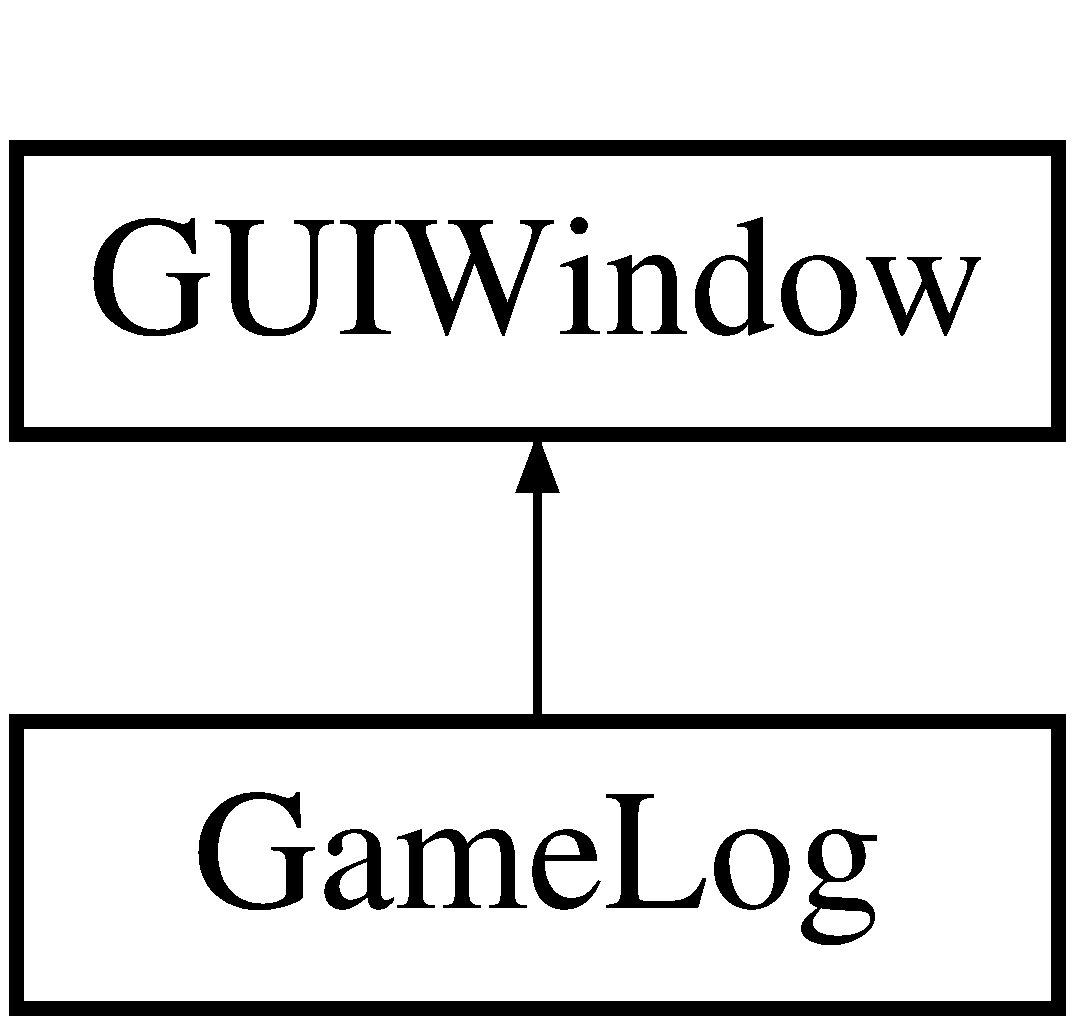
\includegraphics[height=2.000000cm]{class_game_log}
\end{center}
\end{figure}
\subsection*{Public Member Functions}
\begin{DoxyCompactItemize}
\item 
\hyperlink{class_game_log_ab191324ccee35626545525f4ac2d689c}{Game\+Log} ()
\begin{DoxyCompactList}\small\item\em Constructor. \end{DoxyCompactList}\item 
\hyperlink{class_game_log_a3c93bc37578b43b929cb363aa71ab29d}{$\sim$\+Game\+Log} ()=default
\begin{DoxyCompactList}\small\item\em Destructor. \end{DoxyCompactList}\item 
void \hyperlink{class_game_log_a8e8630c1d2b3899de9a90473fd46c415}{clear} ()
\begin{DoxyCompactList}\small\item\em Clears the game\textquotesingle{}s log by deleting all it\textquotesingle{}s entries. \end{DoxyCompactList}\item 
void \hyperlink{class_game_log_a007b6ad87e6278e0902789efb6518227}{print} (const std\+::string \&)
\begin{DoxyCompactList}\small\item\em Prints a string to the game\textquotesingle{}s log. \end{DoxyCompactList}\item 
void \hyperlink{class_game_log_aac1f55f5650514bfa1801e4a54c2d3ac}{set\+\_\+history} (tdt\+::uint)
\begin{DoxyCompactList}\small\item\em Sets the amount of entries kept in the game\textquotesingle{}s log. \end{DoxyCompactList}\item 
tdt\+::uint \hyperlink{class_game_log_a48daa6d325c09b6e972f5f6cab81747f}{get\+\_\+history} () const 
\begin{DoxyCompactList}\small\item\em Returns the amoung of entries kept in the game\textquotesingle{}s log. \end{DoxyCompactList}\end{DoxyCompactItemize}
\subsection*{Protected Member Functions}
\begin{DoxyCompactItemize}
\item 
void \hyperlink{class_game_log_a0b7b3e3cfc91e0b433abdfd286c22b58}{init\+\_\+} () override
\begin{DoxyCompactList}\small\item\em Initializes the game log (called by parent\textquotesingle{}s init). \end{DoxyCompactList}\end{DoxyCompactItemize}
\subsection*{Private Attributes}
\begin{DoxyCompactItemize}
\item 
tdt\+::uint \hyperlink{class_game_log_aeb1a5ef1aada991b96ec36d10ad04e38}{log\+\_\+history\+\_\+}
\begin{DoxyCompactList}\small\item\em Number of entires kept in the game log. \end{DoxyCompactList}\item 
C\+E\+G\+U\+I\+::\+Listbox $\ast$ \hyperlink{class_game_log_aa0a4060d39bd5543aa93c8336bc04d6d}{log\+\_\+}
\begin{DoxyCompactList}\small\item\em Pointer to the log window for easy access (as it might get called quite often, this will avoid frequent lookups). \end{DoxyCompactList}\end{DoxyCompactItemize}
\subsection*{Additional Inherited Members}


\subsection{Detailed Description}
Class representing the log window used to show messages to the player. 

(No space for gold, enemies attacking etc.) \begin{DoxyNote}{Note}
For debug/technical etc messages, see the \hyperlink{class_console}{Console} class. 
\end{DoxyNote}


Definition at line 15 of file Game\+Log.\+hpp.



\subsection{Constructor \& Destructor Documentation}
\index{Game\+Log@{Game\+Log}!Game\+Log@{Game\+Log}}
\index{Game\+Log@{Game\+Log}!Game\+Log@{Game\+Log}}
\subsubsection[{\texorpdfstring{Game\+Log()}{GameLog()}}]{\setlength{\rightskip}{0pt plus 5cm}Game\+Log\+::\+Game\+Log (
\begin{DoxyParamCaption}
{}
\end{DoxyParamCaption}
)}\hypertarget{class_game_log_ab191324ccee35626545525f4ac2d689c}{}\label{class_game_log_ab191324ccee35626545525f4ac2d689c}


Constructor. 



Definition at line 4 of file Game\+Log.\+cpp.

\index{Game\+Log@{Game\+Log}!````~Game\+Log@{$\sim$\+Game\+Log}}
\index{````~Game\+Log@{$\sim$\+Game\+Log}!Game\+Log@{Game\+Log}}
\subsubsection[{\texorpdfstring{$\sim$\+Game\+Log()=default}{~GameLog()=default}}]{\setlength{\rightskip}{0pt plus 5cm}Game\+Log\+::$\sim$\+Game\+Log (
\begin{DoxyParamCaption}
{}
\end{DoxyParamCaption}
)\hspace{0.3cm}{\ttfamily [default]}}\hypertarget{class_game_log_a3c93bc37578b43b929cb363aa71ab29d}{}\label{class_game_log_a3c93bc37578b43b929cb363aa71ab29d}


Destructor. 



\subsection{Member Function Documentation}
\index{Game\+Log@{Game\+Log}!clear@{clear}}
\index{clear@{clear}!Game\+Log@{Game\+Log}}
\subsubsection[{\texorpdfstring{clear()}{clear()}}]{\setlength{\rightskip}{0pt plus 5cm}void Game\+Log\+::clear (
\begin{DoxyParamCaption}
{}
\end{DoxyParamCaption}
)}\hypertarget{class_game_log_a8e8630c1d2b3899de9a90473fd46c415}{}\label{class_game_log_a8e8630c1d2b3899de9a90473fd46c415}


Clears the game\textquotesingle{}s log by deleting all it\textquotesingle{}s entries. 



Definition at line 8 of file Game\+Log.\+cpp.

\index{Game\+Log@{Game\+Log}!get\+\_\+history@{get\+\_\+history}}
\index{get\+\_\+history@{get\+\_\+history}!Game\+Log@{Game\+Log}}
\subsubsection[{\texorpdfstring{get\+\_\+history() const }{get_history() const }}]{\setlength{\rightskip}{0pt plus 5cm}tdt\+::uint Game\+Log\+::get\+\_\+history (
\begin{DoxyParamCaption}
{}
\end{DoxyParamCaption}
) const}\hypertarget{class_game_log_a48daa6d325c09b6e972f5f6cab81747f}{}\label{class_game_log_a48daa6d325c09b6e972f5f6cab81747f}


Returns the amoung of entries kept in the game\textquotesingle{}s log. 



Definition at line 36 of file Game\+Log.\+cpp.

\index{Game\+Log@{Game\+Log}!init\+\_\+@{init\+\_\+}}
\index{init\+\_\+@{init\+\_\+}!Game\+Log@{Game\+Log}}
\subsubsection[{\texorpdfstring{init\+\_\+() override}{init_() override}}]{\setlength{\rightskip}{0pt plus 5cm}void Game\+Log\+::init\+\_\+ (
\begin{DoxyParamCaption}
{}
\end{DoxyParamCaption}
)\hspace{0.3cm}{\ttfamily [override]}, {\ttfamily [protected]}, {\ttfamily [virtual]}}\hypertarget{class_game_log_a0b7b3e3cfc91e0b433abdfd286c22b58}{}\label{class_game_log_a0b7b3e3cfc91e0b433abdfd286c22b58}


Initializes the game log (called by parent\textquotesingle{}s init). 



Implements \hyperlink{class_g_u_i_window_a2a7c011363f401a57a26cc7c7652bdfd}{G\+U\+I\+Window}.



Definition at line 41 of file Game\+Log.\+cpp.

\index{Game\+Log@{Game\+Log}!print@{print}}
\index{print@{print}!Game\+Log@{Game\+Log}}
\subsubsection[{\texorpdfstring{print(const std\+::string \&)}{print(const std::string &)}}]{\setlength{\rightskip}{0pt plus 5cm}void Game\+Log\+::print (
\begin{DoxyParamCaption}
\item[{const std\+::string \&}]{msg}
\end{DoxyParamCaption}
)}\hypertarget{class_game_log_a007b6ad87e6278e0902789efb6518227}{}\label{class_game_log_a007b6ad87e6278e0902789efb6518227}


Prints a string to the game\textquotesingle{}s log. 


\begin{DoxyParams}{Parameters}
{\em String} & to be printed. \\
\hline
\end{DoxyParams}


Definition at line 13 of file Game\+Log.\+cpp.

\index{Game\+Log@{Game\+Log}!set\+\_\+history@{set\+\_\+history}}
\index{set\+\_\+history@{set\+\_\+history}!Game\+Log@{Game\+Log}}
\subsubsection[{\texorpdfstring{set\+\_\+history(tdt\+::uint)}{set_history(tdt::uint)}}]{\setlength{\rightskip}{0pt plus 5cm}void Game\+Log\+::set\+\_\+history (
\begin{DoxyParamCaption}
\item[{tdt\+::uint}]{val}
\end{DoxyParamCaption}
)}\hypertarget{class_game_log_aac1f55f5650514bfa1801e4a54c2d3ac}{}\label{class_game_log_aac1f55f5650514bfa1801e4a54c2d3ac}


Sets the amount of entries kept in the game\textquotesingle{}s log. 


\begin{DoxyParams}{Parameters}
{\em The} & new log history. \\
\hline
\end{DoxyParams}


Definition at line 31 of file Game\+Log.\+cpp.



\subsection{Member Data Documentation}
\index{Game\+Log@{Game\+Log}!log\+\_\+@{log\+\_\+}}
\index{log\+\_\+@{log\+\_\+}!Game\+Log@{Game\+Log}}
\subsubsection[{\texorpdfstring{log\+\_\+}{log_}}]{\setlength{\rightskip}{0pt plus 5cm}C\+E\+G\+U\+I\+::\+Listbox$\ast$ Game\+Log\+::log\+\_\+\hspace{0.3cm}{\ttfamily [private]}}\hypertarget{class_game_log_aa0a4060d39bd5543aa93c8336bc04d6d}{}\label{class_game_log_aa0a4060d39bd5543aa93c8336bc04d6d}


Pointer to the log window for easy access (as it might get called quite often, this will avoid frequent lookups). 



Definition at line 66 of file Game\+Log.\+hpp.

\index{Game\+Log@{Game\+Log}!log\+\_\+history\+\_\+@{log\+\_\+history\+\_\+}}
\index{log\+\_\+history\+\_\+@{log\+\_\+history\+\_\+}!Game\+Log@{Game\+Log}}
\subsubsection[{\texorpdfstring{log\+\_\+history\+\_\+}{log_history_}}]{\setlength{\rightskip}{0pt plus 5cm}tdt\+::uint Game\+Log\+::log\+\_\+history\+\_\+\hspace{0.3cm}{\ttfamily [private]}}\hypertarget{class_game_log_aeb1a5ef1aada991b96ec36d10ad04e38}{}\label{class_game_log_aeb1a5ef1aada991b96ec36d10ad04e38}


Number of entires kept in the game log. 



Definition at line 60 of file Game\+Log.\+hpp.



The documentation for this class was generated from the following files\+:\begin{DoxyCompactItemize}
\item 
gui/Game\+Log.\+hpp\item 
gui/Game\+Log.\+cpp\end{DoxyCompactItemize}

\hypertarget{class_game_serializer}{}\section{Game\+Serializer Class Reference}
\label{class_game_serializer}\index{Game\+Serializer@{Game\+Serializer}}


Class that is used to save (by using Lua code generation) and loading the game (by executing said code).  




{\ttfamily \#include $<$Game\+Serializer.\+hpp$>$}

\subsection*{Public Member Functions}
\begin{DoxyCompactItemize}
\item 
\hyperlink{class_game_serializer_a2729d91f839374a45ffb009db9bf7da3}{Game\+Serializer} (\hyperlink{class_entity_system}{Entity\+System} \&)
\begin{DoxyCompactList}\small\item\em Constructor. \end{DoxyCompactList}\item 
\hyperlink{class_game_serializer_abff94e1ff460d5793747a662ffd08851}{$\sim$\+Game\+Serializer} ()
\begin{DoxyCompactList}\small\item\em Destructor. \end{DoxyCompactList}\item 
void \hyperlink{class_game_serializer_aa57bfc3a1490bbbf73c75daa5ab06644}{save\+\_\+game} (\hyperlink{class_game}{Game} \&, const std\+::string \&=\char`\"{}quick\+\_\+save\char`\"{})
\begin{DoxyCompactList}\small\item\em Creates a Lua script that is to be used as a save file by serializing every entity into a sequence of commands that create this entity from scratch when executed. \end{DoxyCompactList}\item 
void \hyperlink{class_game_serializer_a4f1a6c9202608b390c15c25efc6f2987}{load\+\_\+game} (\hyperlink{class_game}{Game} \&, const std\+::string \&=\char`\"{}quick\+\_\+save\char`\"{})
\begin{DoxyCompactList}\small\item\em Executes a given Lua script containing a serialized game, effectively restoring the state of that game. \end{DoxyCompactList}\end{DoxyCompactItemize}
\subsection*{Private Types}
\begin{DoxyCompactItemize}
\item 
typedef void(Game\+Serializer\+::$\ast$ {\bfseries Serializer\+Func\+Ptr}) (tdt\+::uint, const std\+::string \&)\hypertarget{class_game_serializer_abd56146db26ebda55e7564b630d4abd9}{}\label{class_game_serializer_abd56146db26ebda55e7564b630d4abd9}

\end{DoxyCompactItemize}
\subsection*{Private Member Functions}
\begin{DoxyCompactItemize}
\item 
void \hyperlink{class_game_serializer_a828057a03cbf68491db761b34fc41658}{save\+\_\+tasks} ()
\begin{DoxyCompactList}\small\item\em Adds commands to the save file that assign all tasks (has to be done last). \end{DoxyCompactList}\item 
std\+::string \hyperlink{class_game_serializer_a2beb65f871b5635f5ae0c660615944e8}{save\+\_\+wave\+\_\+system} (\hyperlink{class_game}{Game} \&)
\begin{DoxyCompactList}\small\item\em Returns a string containing commands that will restore the wave system to it\textquotesingle{}s current state. \end{DoxyCompactList}\item 
std\+::string \hyperlink{class_game_serializer_ac200ccdf710ee88a2189b8775f0d2347}{save\+\_\+unlocks} ()
\begin{DoxyCompactList}\small\item\em Returns a string containing commands that will restore the unlock system to it\textquotesingle{}s current state. \end{DoxyCompactList}\item 
{\footnotesize template$<$typename C\+O\+MP $>$ }\\void \hyperlink{class_game_serializer_a56f3943e57b817f99f5787d15802ae81}{save\+\_\+component} (tdt\+::uint, const std\+::string \&)
\begin{DoxyCompactList}\small\item\em Generates code that constructs a single component. \end{DoxyCompactList}\item 
{\footnotesize template$<$$>$ }\\void {\bfseries save\+\_\+component} (tdt\+::uint id, const std\+::string \&tbl\+\_\+name)\hypertarget{class_game_serializer_a2b8f301421ab3d3df49c1b3537ab3b96}{}\label{class_game_serializer_a2b8f301421ab3d3df49c1b3537ab3b96}

\item 
{\footnotesize template$<$$>$ }\\void {\bfseries save\+\_\+component} (tdt\+::uint id, const std\+::string \&tbl\+\_\+name)\hypertarget{class_game_serializer_a2b8f301421ab3d3df49c1b3537ab3b96}{}\label{class_game_serializer_a2b8f301421ab3d3df49c1b3537ab3b96}

\item 
{\footnotesize template$<$$>$ }\\void {\bfseries save\+\_\+component} (tdt\+::uint id, const std\+::string \&tbl\+\_\+name)\hypertarget{class_game_serializer_a2b8f301421ab3d3df49c1b3537ab3b96}{}\label{class_game_serializer_a2b8f301421ab3d3df49c1b3537ab3b96}

\item 
{\footnotesize template$<$$>$ }\\void {\bfseries save\+\_\+component} (tdt\+::uint id, const std\+::string \&tbl\+\_\+name)\hypertarget{class_game_serializer_a2b8f301421ab3d3df49c1b3537ab3b96}{}\label{class_game_serializer_a2b8f301421ab3d3df49c1b3537ab3b96}

\item 
{\footnotesize template$<$$>$ }\\void {\bfseries save\+\_\+component} (tdt\+::uint id, const std\+::string \&tbl\+\_\+name)\hypertarget{class_game_serializer_a2b8f301421ab3d3df49c1b3537ab3b96}{}\label{class_game_serializer_a2b8f301421ab3d3df49c1b3537ab3b96}

\item 
{\footnotesize template$<$$>$ }\\void {\bfseries save\+\_\+component} (tdt\+::uint id, const std\+::string \&tbl\+\_\+name)\hypertarget{class_game_serializer_a2b8f301421ab3d3df49c1b3537ab3b96}{}\label{class_game_serializer_a2b8f301421ab3d3df49c1b3537ab3b96}

\item 
{\footnotesize template$<$$>$ }\\void {\bfseries save\+\_\+component} (tdt\+::uint id, const std\+::string \&tbl\+\_\+name)\hypertarget{class_game_serializer_a2b8f301421ab3d3df49c1b3537ab3b96}{}\label{class_game_serializer_a2b8f301421ab3d3df49c1b3537ab3b96}

\item 
{\footnotesize template$<$$>$ }\\void {\bfseries save\+\_\+component} (tdt\+::uint id, const std\+::string \&tbl\+\_\+name)\hypertarget{class_game_serializer_a2b8f301421ab3d3df49c1b3537ab3b96}{}\label{class_game_serializer_a2b8f301421ab3d3df49c1b3537ab3b96}

\item 
{\footnotesize template$<$$>$ }\\void {\bfseries save\+\_\+component} (tdt\+::uint id, const std\+::string \&tbl\+\_\+name)\hypertarget{class_game_serializer_a2b8f301421ab3d3df49c1b3537ab3b96}{}\label{class_game_serializer_a2b8f301421ab3d3df49c1b3537ab3b96}

\item 
{\footnotesize template$<$$>$ }\\void {\bfseries save\+\_\+component} (tdt\+::uint id, const std\+::string \&tbl\+\_\+name)\hypertarget{class_game_serializer_a2b8f301421ab3d3df49c1b3537ab3b96}{}\label{class_game_serializer_a2b8f301421ab3d3df49c1b3537ab3b96}

\item 
{\footnotesize template$<$$>$ }\\void {\bfseries save\+\_\+component} (tdt\+::uint id, const std\+::string \&tbl\+\_\+name)\hypertarget{class_game_serializer_a2b8f301421ab3d3df49c1b3537ab3b96}{}\label{class_game_serializer_a2b8f301421ab3d3df49c1b3537ab3b96}

\item 
{\footnotesize template$<$$>$ }\\void {\bfseries save\+\_\+component} (tdt\+::uint id, const std\+::string \&tbl\+\_\+name)\hypertarget{class_game_serializer_a2b8f301421ab3d3df49c1b3537ab3b96}{}\label{class_game_serializer_a2b8f301421ab3d3df49c1b3537ab3b96}

\item 
{\footnotesize template$<$$>$ }\\void {\bfseries save\+\_\+component} (tdt\+::uint id, const std\+::string \&tbl\+\_\+name)\hypertarget{class_game_serializer_a2b8f301421ab3d3df49c1b3537ab3b96}{}\label{class_game_serializer_a2b8f301421ab3d3df49c1b3537ab3b96}

\item 
{\footnotesize template$<$$>$ }\\void {\bfseries save\+\_\+component} (tdt\+::uint id, const std\+::string \&tbl\+\_\+name)\hypertarget{class_game_serializer_a2b8f301421ab3d3df49c1b3537ab3b96}{}\label{class_game_serializer_a2b8f301421ab3d3df49c1b3537ab3b96}

\item 
{\footnotesize template$<$$>$ }\\void {\bfseries save\+\_\+component} (tdt\+::uint id, const std\+::string \&tbl\+\_\+name)\hypertarget{class_game_serializer_a2b8f301421ab3d3df49c1b3537ab3b96}{}\label{class_game_serializer_a2b8f301421ab3d3df49c1b3537ab3b96}

\item 
{\footnotesize template$<$$>$ }\\void {\bfseries save\+\_\+component} (tdt\+::uint id, const std\+::string \&tbl\+\_\+name)\hypertarget{class_game_serializer_a2b8f301421ab3d3df49c1b3537ab3b96}{}\label{class_game_serializer_a2b8f301421ab3d3df49c1b3537ab3b96}

\item 
{\footnotesize template$<$$>$ }\\void {\bfseries save\+\_\+component} (tdt\+::uint id, const std\+::string \&tbl\+\_\+name)\hypertarget{class_game_serializer_a2b8f301421ab3d3df49c1b3537ab3b96}{}\label{class_game_serializer_a2b8f301421ab3d3df49c1b3537ab3b96}

\item 
{\footnotesize template$<$$>$ }\\void {\bfseries save\+\_\+component} (tdt\+::uint id, const std\+::string \&tbl\+\_\+name)\hypertarget{class_game_serializer_a2b8f301421ab3d3df49c1b3537ab3b96}{}\label{class_game_serializer_a2b8f301421ab3d3df49c1b3537ab3b96}

\item 
{\footnotesize template$<$$>$ }\\void {\bfseries save\+\_\+component} (tdt\+::uint id, const std\+::string \&tbl\+\_\+name)\hypertarget{class_game_serializer_a2b8f301421ab3d3df49c1b3537ab3b96}{}\label{class_game_serializer_a2b8f301421ab3d3df49c1b3537ab3b96}

\item 
{\footnotesize template$<$$>$ }\\void {\bfseries save\+\_\+component} (tdt\+::uint id, const std\+::string \&tbl\+\_\+name)\hypertarget{class_game_serializer_a2b8f301421ab3d3df49c1b3537ab3b96}{}\label{class_game_serializer_a2b8f301421ab3d3df49c1b3537ab3b96}

\item 
{\footnotesize template$<$$>$ }\\void {\bfseries save\+\_\+component} (tdt\+::uint id, const std\+::string \&tbl\+\_\+name)\hypertarget{class_game_serializer_a2b8f301421ab3d3df49c1b3537ab3b96}{}\label{class_game_serializer_a2b8f301421ab3d3df49c1b3537ab3b96}

\item 
{\footnotesize template$<$$>$ }\\void {\bfseries save\+\_\+component} (tdt\+::uint id, const std\+::string \&tbl\+\_\+name)\hypertarget{class_game_serializer_a2b8f301421ab3d3df49c1b3537ab3b96}{}\label{class_game_serializer_a2b8f301421ab3d3df49c1b3537ab3b96}

\item 
{\footnotesize template$<$$>$ }\\void {\bfseries save\+\_\+component} (tdt\+::uint id, const std\+::string \&tbl\+\_\+name)\hypertarget{class_game_serializer_a2b8f301421ab3d3df49c1b3537ab3b96}{}\label{class_game_serializer_a2b8f301421ab3d3df49c1b3537ab3b96}

\item 
{\footnotesize template$<$$>$ }\\void {\bfseries save\+\_\+component} (tdt\+::uint id, const std\+::string \&tbl\+\_\+name)\hypertarget{class_game_serializer_a2b8f301421ab3d3df49c1b3537ab3b96}{}\label{class_game_serializer_a2b8f301421ab3d3df49c1b3537ab3b96}

\item 
{\footnotesize template$<$$>$ }\\void {\bfseries save\+\_\+component} (tdt\+::uint id, const std\+::string \&tbl\+\_\+name)\hypertarget{class_game_serializer_a2b8f301421ab3d3df49c1b3537ab3b96}{}\label{class_game_serializer_a2b8f301421ab3d3df49c1b3537ab3b96}

\item 
{\footnotesize template$<$$>$ }\\void {\bfseries save\+\_\+component} (tdt\+::uint id, const std\+::string \&tbl\+\_\+name)\hypertarget{class_game_serializer_a2b8f301421ab3d3df49c1b3537ab3b96}{}\label{class_game_serializer_a2b8f301421ab3d3df49c1b3537ab3b96}

\item 
{\footnotesize template$<$$>$ }\\void {\bfseries save\+\_\+component} (tdt\+::uint id, const std\+::string \&tbl\+\_\+name)\hypertarget{class_game_serializer_a2b8f301421ab3d3df49c1b3537ab3b96}{}\label{class_game_serializer_a2b8f301421ab3d3df49c1b3537ab3b96}

\item 
{\footnotesize template$<$$>$ }\\void {\bfseries save\+\_\+component} (tdt\+::uint id, const std\+::string \&tbl\+\_\+name)\hypertarget{class_game_serializer_a2b8f301421ab3d3df49c1b3537ab3b96}{}\label{class_game_serializer_a2b8f301421ab3d3df49c1b3537ab3b96}

\item 
{\footnotesize template$<$$>$ }\\void {\bfseries save\+\_\+component} (tdt\+::uint id, const std\+::string \&tbl\+\_\+name)\hypertarget{class_game_serializer_a2b8f301421ab3d3df49c1b3537ab3b96}{}\label{class_game_serializer_a2b8f301421ab3d3df49c1b3537ab3b96}

\item 
{\footnotesize template$<$$>$ }\\void {\bfseries save\+\_\+component} (tdt\+::uint id, const std\+::string \&tbl\+\_\+name)\hypertarget{class_game_serializer_a2b8f301421ab3d3df49c1b3537ab3b96}{}\label{class_game_serializer_a2b8f301421ab3d3df49c1b3537ab3b96}

\item 
{\footnotesize template$<$$>$ }\\void {\bfseries save\+\_\+component} (tdt\+::uint id, const std\+::string \&tbl\+\_\+name)\hypertarget{class_game_serializer_a2b8f301421ab3d3df49c1b3537ab3b96}{}\label{class_game_serializer_a2b8f301421ab3d3df49c1b3537ab3b96}

\item 
{\footnotesize template$<$$>$ }\\void {\bfseries save\+\_\+component} (tdt\+::uint id, const std\+::string \&tbl\+\_\+name)\hypertarget{class_game_serializer_a2b8f301421ab3d3df49c1b3537ab3b96}{}\label{class_game_serializer_a2b8f301421ab3d3df49c1b3537ab3b96}

\item 
{\footnotesize template$<$$>$ }\\void {\bfseries save\+\_\+component} (tdt\+::uint id, const std\+::string \&tbl\+\_\+name)\hypertarget{class_game_serializer_a2b8f301421ab3d3df49c1b3537ab3b96}{}\label{class_game_serializer_a2b8f301421ab3d3df49c1b3537ab3b96}

\item 
{\footnotesize template$<$$>$ }\\void {\bfseries save\+\_\+component} (tdt\+::uint id, const std\+::string \&tbl\+\_\+name)\hypertarget{class_game_serializer_a2b8f301421ab3d3df49c1b3537ab3b96}{}\label{class_game_serializer_a2b8f301421ab3d3df49c1b3537ab3b96}

\item 
{\footnotesize template$<$$>$ }\\void {\bfseries save\+\_\+component} (tdt\+::uint id, const std\+::string \&tbl\+\_\+name)\hypertarget{class_game_serializer_a2b8f301421ab3d3df49c1b3537ab3b96}{}\label{class_game_serializer_a2b8f301421ab3d3df49c1b3537ab3b96}

\item 
{\footnotesize template$<$$>$ }\\void {\bfseries save\+\_\+component} (tdt\+::uint id, const std\+::string \&tbl\+\_\+name)\hypertarget{class_game_serializer_a2b8f301421ab3d3df49c1b3537ab3b96}{}\label{class_game_serializer_a2b8f301421ab3d3df49c1b3537ab3b96}

\item 
{\footnotesize template$<$$>$ }\\void {\bfseries save\+\_\+component} (tdt\+::uint id, const std\+::string \&tbl\+\_\+name)\hypertarget{class_game_serializer_a2b8f301421ab3d3df49c1b3537ab3b96}{}\label{class_game_serializer_a2b8f301421ab3d3df49c1b3537ab3b96}

\item 
{\footnotesize template$<$$>$ }\\void {\bfseries save\+\_\+component} (tdt\+::uint id, const std\+::string \&tbl\+\_\+name)\hypertarget{class_game_serializer_a2b8f301421ab3d3df49c1b3537ab3b96}{}\label{class_game_serializer_a2b8f301421ab3d3df49c1b3537ab3b96}

\item 
{\footnotesize template$<$$>$ }\\void {\bfseries save\+\_\+component} (tdt\+::uint id, const std\+::string \&tbl\+\_\+name)\hypertarget{class_game_serializer_a2b8f301421ab3d3df49c1b3537ab3b96}{}\label{class_game_serializer_a2b8f301421ab3d3df49c1b3537ab3b96}

\end{DoxyCompactItemize}
\subsection*{Private Attributes}
\begin{DoxyCompactItemize}
\item 
\hyperlink{class_entity_system}{Entity\+System} \& \hyperlink{class_game_serializer_a28c5d447a195faa9da04f19b26617b16}{entities\+\_\+}
\begin{DoxyCompactList}\small\item\em Reference to the game\textquotesingle{}s entity system, used for component access. \end{DoxyCompactList}\item 
\hyperlink{classlpp_1_1_script}{lpp\+::\+Script} \& \hyperlink{class_game_serializer_a96a50f04014f8378c8cb30321107ef25}{script\+\_\+}
\begin{DoxyCompactList}\small\item\em Reference to the \hyperlink{classlpp_1_1_script}{lpp\+::\+Script} singleton for easy use. \end{DoxyCompactList}\item 
std\+::vector$<$ std\+::pair$<$ tdt\+::uint, tdt\+::uint $>$ $>$ \hyperlink{class_game_serializer_a556001cdf90fde90c842100db0cda29a}{task\+\_\+pairs\+\_\+}
\begin{DoxyCompactList}\small\item\em Contains entity -\/ task pairs that should be added in the save\+\_\+tasks method. \end{DoxyCompactList}\item 
std\+::ofstream \hyperlink{class_game_serializer_a85c282b5993050dba19dc760ea33b536}{file\+\_\+}
\begin{DoxyCompactList}\small\item\em Main file stream (no need for ifstream, since loading is done through Lua). \end{DoxyCompactList}\item 
std\+::vector$<$ std\+::string $>$ \hyperlink{class_game_serializer_a0f6b379c053d77bb9df6bc8004280ccd}{save\+\_\+entities\+\_\+}
\begin{DoxyCompactList}\small\item\em Auxiliary vectors that allows to place entity creation at the top (so no entity variables are nil when loading a game) and component definitions at the bottom. \end{DoxyCompactList}\item 
std\+::vector$<$ std\+::string $>$ {\bfseries save\+\_\+components\+\_\+}\hypertarget{class_game_serializer_a7b64dc19195f0fe7796cb15765162a0f}{}\label{class_game_serializer_a7b64dc19195f0fe7796cb15765162a0f}

\item 
std\+::array$<$ Serializer\+Func\+Ptr, Component\+::count $>$ \hyperlink{class_game_serializer_a0baa52b5d165843f904c9f72aac5a640}{serializers\+\_\+}
\begin{DoxyCompactList}\small\item\em Pointers to the different save\+\_\+component instances allowing for easy runtime differencing between components. \end{DoxyCompactList}\end{DoxyCompactItemize}


\subsection{Detailed Description}
Class that is used to save (by using Lua code generation) and loading the game (by executing said code). 

Definition at line 22 of file Game\+Serializer.\+hpp.



\subsection{Constructor \& Destructor Documentation}
\index{Game\+Serializer@{Game\+Serializer}!Game\+Serializer@{Game\+Serializer}}
\index{Game\+Serializer@{Game\+Serializer}!Game\+Serializer@{Game\+Serializer}}
\subsubsection[{\texorpdfstring{Game\+Serializer(\+Entity\+System \&)}{GameSerializer(EntitySystem &)}}]{\setlength{\rightskip}{0pt plus 5cm}Game\+Serializer\+::\+Game\+Serializer (
\begin{DoxyParamCaption}
\item[{{\bf Entity\+System} \&}]{ents}
\end{DoxyParamCaption}
)}\hypertarget{class_game_serializer_a2729d91f839374a45ffb009db9bf7da3}{}\label{class_game_serializer_a2729d91f839374a45ffb009db9bf7da3}


Constructor. 


\begin{DoxyParams}{Parameters}
{\em Reference} & to the game\textquotesingle{}s entity system. \\
\hline
\end{DoxyParams}


Definition at line 17 of file Game\+Serializer.\+cpp.

\index{Game\+Serializer@{Game\+Serializer}!````~Game\+Serializer@{$\sim$\+Game\+Serializer}}
\index{````~Game\+Serializer@{$\sim$\+Game\+Serializer}!Game\+Serializer@{Game\+Serializer}}
\subsubsection[{\texorpdfstring{$\sim$\+Game\+Serializer()}{~GameSerializer()}}]{\setlength{\rightskip}{0pt plus 5cm}Game\+Serializer\+::$\sim$\+Game\+Serializer (
\begin{DoxyParamCaption}
{}
\end{DoxyParamCaption}
)\hspace{0.3cm}{\ttfamily [inline]}}\hypertarget{class_game_serializer_abff94e1ff460d5793747a662ffd08851}{}\label{class_game_serializer_abff94e1ff460d5793747a662ffd08851}


Destructor. 



Definition at line 35 of file Game\+Serializer.\+hpp.



\subsection{Member Function Documentation}
\index{Game\+Serializer@{Game\+Serializer}!load\+\_\+game@{load\+\_\+game}}
\index{load\+\_\+game@{load\+\_\+game}!Game\+Serializer@{Game\+Serializer}}
\subsubsection[{\texorpdfstring{load\+\_\+game(\+Game \&, const std\+::string \&=""quick\+\_\+save"")}{load_game(Game &, const std::string &="quick_save")}}]{\setlength{\rightskip}{0pt plus 5cm}void Game\+Serializer\+::load\+\_\+game (
\begin{DoxyParamCaption}
\item[{{\bf Game} \&}]{game, }
\item[{const std\+::string \&}]{fname = {\ttfamily \char`\"{}quick\+\_\+save\char`\"{}}}
\end{DoxyParamCaption}
)}\hypertarget{class_game_serializer_a4f1a6c9202608b390c15c25efc6f2987}{}\label{class_game_serializer_a4f1a6c9202608b390c15c25efc6f2987}


Executes a given Lua script containing a serialized game, effectively restoring the state of that game. 


\begin{DoxyParams}{Parameters}
{\em Reference} & to the game object (currently used for console entries, but might be used more in the future). \\
\hline
{\em Name} & of the save file to load. \\
\hline
\end{DoxyParams}


Definition at line 142 of file Game\+Serializer.\+cpp.

\index{Game\+Serializer@{Game\+Serializer}!save\+\_\+component@{save\+\_\+component}}
\index{save\+\_\+component@{save\+\_\+component}!Game\+Serializer@{Game\+Serializer}}
\subsubsection[{\texorpdfstring{save\+\_\+component(tdt\+::uint, const std\+::string \&)}{save_component(tdt::uint, const std::string &)}}]{\setlength{\rightskip}{0pt plus 5cm}template$<$typename C\+O\+MP $>$ void Game\+Serializer\+::save\+\_\+component (
\begin{DoxyParamCaption}
\item[{tdt\+::uint}]{, }
\item[{const std\+::string \&}]{}
\end{DoxyParamCaption}
)\hspace{0.3cm}{\ttfamily [private]}}\hypertarget{class_game_serializer_a56f3943e57b817f99f5787d15802ae81}{}\label{class_game_serializer_a56f3943e57b817f99f5787d15802ae81}


Generates code that constructs a single component. 


\begin{DoxyParams}{Parameters}
{\em ID} & of the component to serialize (type specialized as template argument). \\
\hline
{\em Name} & of the variable already in the save file that holds the new ID. \\
\hline
\end{DoxyParams}
\index{Game\+Serializer@{Game\+Serializer}!save\+\_\+game@{save\+\_\+game}}
\index{save\+\_\+game@{save\+\_\+game}!Game\+Serializer@{Game\+Serializer}}
\subsubsection[{\texorpdfstring{save\+\_\+game(\+Game \&, const std\+::string \&=""quick\+\_\+save"")}{save_game(Game &, const std::string &="quick_save")}}]{\setlength{\rightskip}{0pt plus 5cm}void Game\+Serializer\+::save\+\_\+game (
\begin{DoxyParamCaption}
\item[{{\bf Game} \&}]{game, }
\item[{const std\+::string \&}]{fname = {\ttfamily \char`\"{}quick\+\_\+save\char`\"{}}}
\end{DoxyParamCaption}
)}\hypertarget{class_game_serializer_aa57bfc3a1490bbbf73c75daa5ab06644}{}\label{class_game_serializer_aa57bfc3a1490bbbf73c75daa5ab06644}


Creates a Lua script that is to be used as a save file by serializing every entity into a sequence of commands that create this entity from scratch when executed. 


\begin{DoxyParams}{Parameters}
{\em Reference} & to the \hyperlink{class_game}{Game} object (to be able to save all necessary data). \\
\hline
{\em Name} & of the save file. \\
\hline
\end{DoxyParams}


Definition at line 64 of file Game\+Serializer.\+cpp.

\index{Game\+Serializer@{Game\+Serializer}!save\+\_\+tasks@{save\+\_\+tasks}}
\index{save\+\_\+tasks@{save\+\_\+tasks}!Game\+Serializer@{Game\+Serializer}}
\subsubsection[{\texorpdfstring{save\+\_\+tasks()}{save_tasks()}}]{\setlength{\rightskip}{0pt plus 5cm}void Game\+Serializer\+::save\+\_\+tasks (
\begin{DoxyParamCaption}
{}
\end{DoxyParamCaption}
)\hspace{0.3cm}{\ttfamily [private]}}\hypertarget{class_game_serializer_a828057a03cbf68491db761b34fc41658}{}\label{class_game_serializer_a828057a03cbf68491db761b34fc41658}


Adds commands to the save file that assign all tasks (has to be done last). 



Definition at line 172 of file Game\+Serializer.\+cpp.

\index{Game\+Serializer@{Game\+Serializer}!save\+\_\+unlocks@{save\+\_\+unlocks}}
\index{save\+\_\+unlocks@{save\+\_\+unlocks}!Game\+Serializer@{Game\+Serializer}}
\subsubsection[{\texorpdfstring{save\+\_\+unlocks()}{save_unlocks()}}]{\setlength{\rightskip}{0pt plus 5cm}std\+::string Game\+Serializer\+::save\+\_\+unlocks (
\begin{DoxyParamCaption}
{}
\end{DoxyParamCaption}
)\hspace{0.3cm}{\ttfamily [private]}}\hypertarget{class_game_serializer_ac200ccdf710ee88a2189b8775f0d2347}{}\label{class_game_serializer_ac200ccdf710ee88a2189b8775f0d2347}


Returns a string containing commands that will restore the unlock system to it\textquotesingle{}s current state. 



Definition at line 213 of file Game\+Serializer.\+cpp.

\index{Game\+Serializer@{Game\+Serializer}!save\+\_\+wave\+\_\+system@{save\+\_\+wave\+\_\+system}}
\index{save\+\_\+wave\+\_\+system@{save\+\_\+wave\+\_\+system}!Game\+Serializer@{Game\+Serializer}}
\subsubsection[{\texorpdfstring{save\+\_\+wave\+\_\+system(\+Game \&)}{save_wave_system(Game &)}}]{\setlength{\rightskip}{0pt plus 5cm}std\+::string Game\+Serializer\+::save\+\_\+wave\+\_\+system (
\begin{DoxyParamCaption}
\item[{{\bf Game} \&}]{game}
\end{DoxyParamCaption}
)\hspace{0.3cm}{\ttfamily [private]}}\hypertarget{class_game_serializer_a2beb65f871b5635f5ae0c660615944e8}{}\label{class_game_serializer_a2beb65f871b5635f5ae0c660615944e8}


Returns a string containing commands that will restore the wave system to it\textquotesingle{}s current state. 


\begin{DoxyParams}{Parameters}
{\em Reference} & to the game object that contains the wave system. \\
\hline
\end{DoxyParams}


Definition at line 183 of file Game\+Serializer.\+cpp.



\subsection{Member Data Documentation}
\index{Game\+Serializer@{Game\+Serializer}!entities\+\_\+@{entities\+\_\+}}
\index{entities\+\_\+@{entities\+\_\+}!Game\+Serializer@{Game\+Serializer}}
\subsubsection[{\texorpdfstring{entities\+\_\+}{entities_}}]{\setlength{\rightskip}{0pt plus 5cm}{\bf Entity\+System}\& Game\+Serializer\+::entities\+\_\+\hspace{0.3cm}{\ttfamily [private]}}\hypertarget{class_game_serializer_a28c5d447a195faa9da04f19b26617b16}{}\label{class_game_serializer_a28c5d447a195faa9da04f19b26617b16}


Reference to the game\textquotesingle{}s entity system, used for component access. 



Definition at line 85 of file Game\+Serializer.\+hpp.

\index{Game\+Serializer@{Game\+Serializer}!file\+\_\+@{file\+\_\+}}
\index{file\+\_\+@{file\+\_\+}!Game\+Serializer@{Game\+Serializer}}
\subsubsection[{\texorpdfstring{file\+\_\+}{file_}}]{\setlength{\rightskip}{0pt plus 5cm}std\+::ofstream Game\+Serializer\+::file\+\_\+\hspace{0.3cm}{\ttfamily [private]}}\hypertarget{class_game_serializer_a85c282b5993050dba19dc760ea33b536}{}\label{class_game_serializer_a85c282b5993050dba19dc760ea33b536}


Main file stream (no need for ifstream, since loading is done through Lua). 



Definition at line 100 of file Game\+Serializer.\+hpp.

\index{Game\+Serializer@{Game\+Serializer}!save\+\_\+entities\+\_\+@{save\+\_\+entities\+\_\+}}
\index{save\+\_\+entities\+\_\+@{save\+\_\+entities\+\_\+}!Game\+Serializer@{Game\+Serializer}}
\subsubsection[{\texorpdfstring{save\+\_\+entities\+\_\+}{save_entities_}}]{\setlength{\rightskip}{0pt plus 5cm}std\+::vector$<$std\+::string$>$ Game\+Serializer\+::save\+\_\+entities\+\_\+\hspace{0.3cm}{\ttfamily [private]}}\hypertarget{class_game_serializer_a0f6b379c053d77bb9df6bc8004280ccd}{}\label{class_game_serializer_a0f6b379c053d77bb9df6bc8004280ccd}


Auxiliary vectors that allows to place entity creation at the top (so no entity variables are nil when loading a game) and component definitions at the bottom. 



Definition at line 106 of file Game\+Serializer.\+hpp.

\index{Game\+Serializer@{Game\+Serializer}!script\+\_\+@{script\+\_\+}}
\index{script\+\_\+@{script\+\_\+}!Game\+Serializer@{Game\+Serializer}}
\subsubsection[{\texorpdfstring{script\+\_\+}{script_}}]{\setlength{\rightskip}{0pt plus 5cm}{\bf lpp\+::\+Script}\& Game\+Serializer\+::script\+\_\+\hspace{0.3cm}{\ttfamily [private]}}\hypertarget{class_game_serializer_a96a50f04014f8378c8cb30321107ef25}{}\label{class_game_serializer_a96a50f04014f8378c8cb30321107ef25}


Reference to the \hyperlink{classlpp_1_1_script}{lpp\+::\+Script} singleton for easy use. 



Definition at line 90 of file Game\+Serializer.\+hpp.

\index{Game\+Serializer@{Game\+Serializer}!serializers\+\_\+@{serializers\+\_\+}}
\index{serializers\+\_\+@{serializers\+\_\+}!Game\+Serializer@{Game\+Serializer}}
\subsubsection[{\texorpdfstring{serializers\+\_\+}{serializers_}}]{\setlength{\rightskip}{0pt plus 5cm}std\+::array$<$Serializer\+Func\+Ptr, Component\+::count$>$ Game\+Serializer\+::serializers\+\_\+\hspace{0.3cm}{\ttfamily [private]}}\hypertarget{class_game_serializer_a0baa52b5d165843f904c9f72aac5a640}{}\label{class_game_serializer_a0baa52b5d165843f904c9f72aac5a640}


Pointers to the different save\+\_\+component instances allowing for easy runtime differencing between components. 



Definition at line 112 of file Game\+Serializer.\+hpp.

\index{Game\+Serializer@{Game\+Serializer}!task\+\_\+pairs\+\_\+@{task\+\_\+pairs\+\_\+}}
\index{task\+\_\+pairs\+\_\+@{task\+\_\+pairs\+\_\+}!Game\+Serializer@{Game\+Serializer}}
\subsubsection[{\texorpdfstring{task\+\_\+pairs\+\_\+}{task_pairs_}}]{\setlength{\rightskip}{0pt plus 5cm}std\+::vector$<$std\+::pair$<$tdt\+::uint, tdt\+::uint$>$ $>$ Game\+Serializer\+::task\+\_\+pairs\+\_\+\hspace{0.3cm}{\ttfamily [private]}}\hypertarget{class_game_serializer_a556001cdf90fde90c842100db0cda29a}{}\label{class_game_serializer_a556001cdf90fde90c842100db0cda29a}


Contains entity -\/ task pairs that should be added in the save\+\_\+tasks method. 



Definition at line 95 of file Game\+Serializer.\+hpp.



The documentation for this class was generated from the following files\+:\begin{DoxyCompactItemize}
\item 
tools/Game\+Serializer.\+hpp\item 
tools/Game\+Serializer.\+cpp\end{DoxyCompactItemize}

\hypertarget{struct_gold_component}{}\section{Gold\+Component Struct Reference}
\label{struct_gold_component}\index{Gold\+Component@{Gold\+Component}}


Represents a gold amount an entity is holding, be it a gold seam, worker minion or gold depository.  




{\ttfamily \#include $<$Components.\+hpp$>$}

\subsection*{Public Member Functions}
\begin{DoxyCompactItemize}
\item 
{\bfseries Gold\+Component} (tdt\+::uint max=0, tdt\+::uint curr=0)\hypertarget{struct_gold_component_ab8447bb12a8325cf3804f5e61a15844b}{}\label{struct_gold_component_ab8447bb12a8325cf3804f5e61a15844b}

\item 
{\bfseries Gold\+Component} (const \hyperlink{struct_gold_component}{Gold\+Component} \&)=default\hypertarget{struct_gold_component_a5d55c80ab002d3c5797699a9c46ede1e}{}\label{struct_gold_component_a5d55c80ab002d3c5797699a9c46ede1e}

\item 
{\bfseries Gold\+Component} (\hyperlink{struct_gold_component}{Gold\+Component} \&\&)=default\hypertarget{struct_gold_component_af33ae4ab76a4b97c46716ff075bab41c}{}\label{struct_gold_component_af33ae4ab76a4b97c46716ff075bab41c}

\item 
\hyperlink{struct_gold_component}{Gold\+Component} \& {\bfseries operator=} (const \hyperlink{struct_gold_component}{Gold\+Component} \&)=default\hypertarget{struct_gold_component_af1f351ee46d01fa436f6d01dba41f00b}{}\label{struct_gold_component_af1f351ee46d01fa436f6d01dba41f00b}

\item 
\hyperlink{struct_gold_component}{Gold\+Component} \& {\bfseries operator=} (\hyperlink{struct_gold_component}{Gold\+Component} \&\&)=default\hypertarget{struct_gold_component_a64718b76ee7ef30300b7df4703c3df0b}{}\label{struct_gold_component_a64718b76ee7ef30300b7df4703c3df0b}

\end{DoxyCompactItemize}
\subsection*{Public Attributes}
\begin{DoxyCompactItemize}
\item 
tdt\+::uint {\bfseries max\+\_\+amount}\hypertarget{struct_gold_component_aea59b958529f948591caddcdbe2208f4}{}\label{struct_gold_component_aea59b958529f948591caddcdbe2208f4}

\item 
tdt\+::uint {\bfseries curr\+\_\+amount}\hypertarget{struct_gold_component_a5b753927743f4fd3736b462f57708439}{}\label{struct_gold_component_a5b753927743f4fd3736b462f57708439}

\end{DoxyCompactItemize}
\subsection*{Static Public Attributes}
\begin{DoxyCompactItemize}
\item 
static constexpr int {\bfseries type} = 21\hypertarget{struct_gold_component_ae3c2d173532fdef10129033d6a0d571e}{}\label{struct_gold_component_ae3c2d173532fdef10129033d6a0d571e}

\end{DoxyCompactItemize}


\subsection{Detailed Description}
Represents a gold amount an entity is holding, be it a gold seam, worker minion or gold depository. 

Definition at line 528 of file Components.\+hpp.



The documentation for this struct was generated from the following file\+:\begin{DoxyCompactItemize}
\item 
Components.\+hpp\end{DoxyCompactItemize}

\hypertarget{struct_graphics_component}{}\section{Graphics\+Component Struct Reference}
\label{struct_graphics_component}\index{Graphics\+Component@{Graphics\+Component}}


Holds info related to the Ogre3D rendering library.  




{\ttfamily \#include $<$Components.\+hpp$>$}

\subsection*{Public Member Functions}
\begin{DoxyCompactItemize}
\item 
{\bfseries Graphics\+Component} (std\+::string \&\&me=\char`\"{}ogrehead.\+mesh\char`\"{}, std\+::string \&\&ma=\char`\"{}Ogre\char`\"{}, bool v=true, bool manual=false, Ogre\+::\+Vector3 sc=Ogre\+::\+Vector3\{0, 0, 0\})\hypertarget{struct_graphics_component_a5d6bd4ff86cca23191caeef3c9da4df1}{}\label{struct_graphics_component_a5d6bd4ff86cca23191caeef3c9da4df1}

\item 
{\bfseries Graphics\+Component} (const \hyperlink{struct_graphics_component}{Graphics\+Component} \&)=default\hypertarget{struct_graphics_component_a920145e7512de4591ca500e318ddd40b}{}\label{struct_graphics_component_a920145e7512de4591ca500e318ddd40b}

\item 
{\bfseries Graphics\+Component} (\hyperlink{struct_graphics_component}{Graphics\+Component} \&\&)=default\hypertarget{struct_graphics_component_a96a0b90002606a5345ca6bf0f6668484}{}\label{struct_graphics_component_a96a0b90002606a5345ca6bf0f6668484}

\item 
\hyperlink{struct_graphics_component}{Graphics\+Component} \& {\bfseries operator=} (const \hyperlink{struct_graphics_component}{Graphics\+Component} \&)=default\hypertarget{struct_graphics_component_ac21301a495f152db325689d6d78dac48}{}\label{struct_graphics_component_ac21301a495f152db325689d6d78dac48}

\item 
\hyperlink{struct_graphics_component}{Graphics\+Component} \& {\bfseries operator=} (\hyperlink{struct_graphics_component}{Graphics\+Component} \&\&)=default\hypertarget{struct_graphics_component_ab28d0c007a37ad7fdf08780bf5c45ba2}{}\label{struct_graphics_component_ab28d0c007a37ad7fdf08780bf5c45ba2}

\end{DoxyCompactItemize}
\subsection*{Public Attributes}
\begin{DoxyCompactItemize}
\item 
std\+::string {\bfseries mesh}\hypertarget{struct_graphics_component_a68d12c02e16e0387acbfc233602a82fa}{}\label{struct_graphics_component_a68d12c02e16e0387acbfc233602a82fa}

\item 
std\+::string {\bfseries material}\hypertarget{struct_graphics_component_a99dec89d4c48b38777ae281458d64316}{}\label{struct_graphics_component_a99dec89d4c48b38777ae281458d64316}

\item 
bool {\bfseries visible}\hypertarget{struct_graphics_component_a1d0c6099159d9864b9447c659ab0a10d}{}\label{struct_graphics_component_a1d0c6099159d9864b9447c659ab0a10d}

\item 
Ogre\+::\+Scene\+Node $\ast$ {\bfseries node}\hypertarget{struct_graphics_component_a4dd94d81cb37863c49a62bea2d8b5288}{}\label{struct_graphics_component_a4dd94d81cb37863c49a62bea2d8b5288}

\item 
Ogre\+::\+Entity $\ast$ {\bfseries entity}\hypertarget{struct_graphics_component_a5e6159f802bae8f873860447549512d5}{}\label{struct_graphics_component_a5e6159f802bae8f873860447549512d5}

\item 
bool {\bfseries manual\+\_\+scaling}\hypertarget{struct_graphics_component_a14a0b1f834e4e4c95feeeabca31d2a93}{}\label{struct_graphics_component_a14a0b1f834e4e4c95feeeabca31d2a93}

\item 
Ogre\+::\+Vector3 {\bfseries scale}\hypertarget{struct_graphics_component_aeec41c43a81a91e2a36855f432fa51cb}{}\label{struct_graphics_component_aeec41c43a81a91e2a36855f432fa51cb}

\end{DoxyCompactItemize}
\subsection*{Static Public Attributes}
\begin{DoxyCompactItemize}
\item 
static constexpr int {\bfseries type} = 3\hypertarget{struct_graphics_component_a74c76950aef60a68476da3bf22d23604}{}\label{struct_graphics_component_a74c76950aef60a68476da3bf22d23604}

\end{DoxyCompactItemize}


\subsection{Detailed Description}
Holds info related to the Ogre3D rendering library. 

Definition at line 101 of file Components.\+hpp.



The documentation for this struct was generated from the following file\+:\begin{DoxyCompactItemize}
\item 
Components.\+hpp\end{DoxyCompactItemize}

\hypertarget{class_graphics_system}{}\section{Graphics\+System Class Reference}
\label{class_graphics_system}\index{Graphics\+System@{Graphics\+System}}


\hyperlink{class_system}{System} that performs all graphics related updates.  




{\ttfamily \#include $<$Graphics\+System.\+hpp$>$}

Inheritance diagram for Graphics\+System\+:\begin{figure}[H]
\begin{center}
\leavevmode
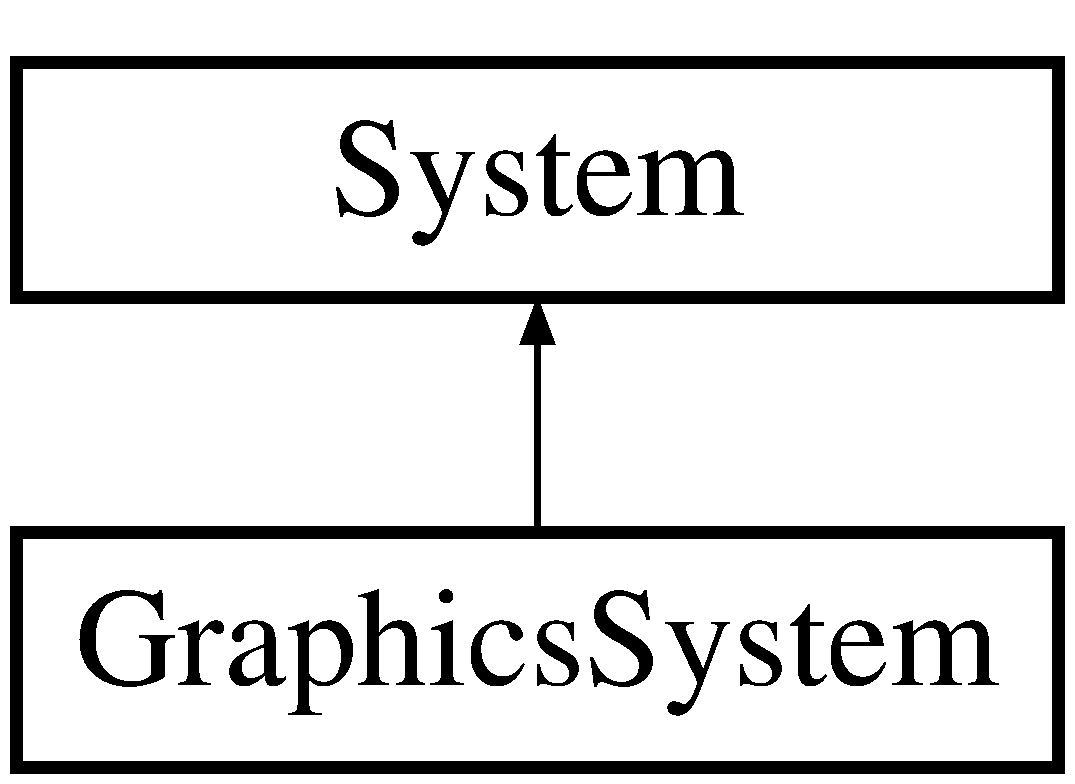
\includegraphics[height=2.000000cm]{class_graphics_system}
\end{center}
\end{figure}
\subsection*{Public Member Functions}
\begin{DoxyCompactItemize}
\item 
\hyperlink{class_graphics_system_a7cac5e6ce0eeb67c1681ffa1f324899d}{Graphics\+System} (\hyperlink{class_entity_system}{Entity\+System} \&)
\begin{DoxyCompactList}\small\item\em Constructor. \end{DoxyCompactList}\item 
\hyperlink{class_graphics_system_a85a733ce82a83bce52c437afb4ebd831}{$\sim$\+Graphics\+System} ()=default
\begin{DoxyCompactList}\small\item\em Destructor. \end{DoxyCompactList}\item 
void \hyperlink{class_graphics_system_a1b5bf7d5928bcc00d90dec8be3866440}{update} (tdt\+::real) override
\begin{DoxyCompactList}\small\item\em Performs all graphics updates. \end{DoxyCompactList}\item 
void \hyperlink{class_graphics_system_ad3138967c974573a11cc486d4718978c}{set\+\_\+update\+\_\+period} (tdt\+::real)
\begin{DoxyCompactList}\small\item\em Sets the time period before the next update. \end{DoxyCompactList}\item 
tdt\+::real \hyperlink{class_graphics_system_afef3488931bd206c0fd89237d1d23f43}{get\+\_\+update\+\_\+period} () const 
\begin{DoxyCompactList}\small\item\em Returns the time period between updates. \end{DoxyCompactList}\end{DoxyCompactItemize}
\subsection*{Private Attributes}
\begin{DoxyCompactItemize}
\item 
\hyperlink{class_entity_system}{Entity\+System} \& \hyperlink{class_graphics_system_ad0471df508e2dc91c475c7460c406023}{entities\+\_\+}
\begin{DoxyCompactList}\small\item\em Entity system that contains entities this system is working with. \end{DoxyCompactList}\item 
tdt\+::real \hyperlink{class_graphics_system_a6100fb67478a56b5c3fb9d994f1a8c0e}{update\+\_\+timer\+\_\+}
\begin{DoxyCompactList}\small\item\em Used to avoid per frame updates and allows dynamic update periods. \end{DoxyCompactList}\item 
tdt\+::real {\bfseries update\+\_\+period\+\_\+}\hypertarget{class_graphics_system_a4763b6bf6e4eb59322a56135b26c99db}{}\label{class_graphics_system_a4763b6bf6e4eb59322a56135b26c99db}

\end{DoxyCompactItemize}


\subsection{Detailed Description}
\hyperlink{class_system}{System} that performs all graphics related updates. 

Definition at line 10 of file Graphics\+System.\+hpp.



\subsection{Constructor \& Destructor Documentation}
\index{Graphics\+System@{Graphics\+System}!Graphics\+System@{Graphics\+System}}
\index{Graphics\+System@{Graphics\+System}!Graphics\+System@{Graphics\+System}}
\subsubsection[{\texorpdfstring{Graphics\+System(\+Entity\+System \&)}{GraphicsSystem(EntitySystem &)}}]{\setlength{\rightskip}{0pt plus 5cm}Graphics\+System\+::\+Graphics\+System (
\begin{DoxyParamCaption}
\item[{{\bf Entity\+System} \&}]{ents}
\end{DoxyParamCaption}
)}\hypertarget{class_graphics_system_a7cac5e6ce0eeb67c1681ffa1f324899d}{}\label{class_graphics_system_a7cac5e6ce0eeb67c1681ffa1f324899d}


Constructor. 


\begin{DoxyParams}{Parameters}
{\em The} & game\textquotesingle{}s entity system. \\
\hline
\end{DoxyParams}


Definition at line 4 of file Graphics\+System.\+cpp.

\index{Graphics\+System@{Graphics\+System}!````~Graphics\+System@{$\sim$\+Graphics\+System}}
\index{````~Graphics\+System@{$\sim$\+Graphics\+System}!Graphics\+System@{Graphics\+System}}
\subsubsection[{\texorpdfstring{$\sim$\+Graphics\+System()=default}{~GraphicsSystem()=default}}]{\setlength{\rightskip}{0pt plus 5cm}Graphics\+System\+::$\sim$\+Graphics\+System (
\begin{DoxyParamCaption}
{}
\end{DoxyParamCaption}
)\hspace{0.3cm}{\ttfamily [default]}}\hypertarget{class_graphics_system_a85a733ce82a83bce52c437afb4ebd831}{}\label{class_graphics_system_a85a733ce82a83bce52c437afb4ebd831}


Destructor. 



\subsection{Member Function Documentation}
\index{Graphics\+System@{Graphics\+System}!get\+\_\+update\+\_\+period@{get\+\_\+update\+\_\+period}}
\index{get\+\_\+update\+\_\+period@{get\+\_\+update\+\_\+period}!Graphics\+System@{Graphics\+System}}
\subsubsection[{\texorpdfstring{get\+\_\+update\+\_\+period() const }{get_update_period() const }}]{\setlength{\rightskip}{0pt plus 5cm}tdt\+::real Graphics\+System\+::get\+\_\+update\+\_\+period (
\begin{DoxyParamCaption}
{}
\end{DoxyParamCaption}
) const}\hypertarget{class_graphics_system_afef3488931bd206c0fd89237d1d23f43}{}\label{class_graphics_system_afef3488931bd206c0fd89237d1d23f43}


Returns the time period between updates. 



Definition at line 45 of file Graphics\+System.\+cpp.

\index{Graphics\+System@{Graphics\+System}!set\+\_\+update\+\_\+period@{set\+\_\+update\+\_\+period}}
\index{set\+\_\+update\+\_\+period@{set\+\_\+update\+\_\+period}!Graphics\+System@{Graphics\+System}}
\subsubsection[{\texorpdfstring{set\+\_\+update\+\_\+period(tdt\+::real)}{set_update_period(tdt::real)}}]{\setlength{\rightskip}{0pt plus 5cm}void Graphics\+System\+::set\+\_\+update\+\_\+period (
\begin{DoxyParamCaption}
\item[{tdt\+::real}]{val}
\end{DoxyParamCaption}
)}\hypertarget{class_graphics_system_ad3138967c974573a11cc486d4718978c}{}\label{class_graphics_system_ad3138967c974573a11cc486d4718978c}


Sets the time period before the next update. 


\begin{DoxyParams}{Parameters}
{\em The} & new period. \\
\hline
\end{DoxyParams}


Definition at line 40 of file Graphics\+System.\+cpp.

\index{Graphics\+System@{Graphics\+System}!update@{update}}
\index{update@{update}!Graphics\+System@{Graphics\+System}}
\subsubsection[{\texorpdfstring{update(tdt\+::real) override}{update(tdt::real) override}}]{\setlength{\rightskip}{0pt plus 5cm}void Graphics\+System\+::update (
\begin{DoxyParamCaption}
\item[{tdt\+::real}]{delta}
\end{DoxyParamCaption}
)\hspace{0.3cm}{\ttfamily [override]}, {\ttfamily [virtual]}}\hypertarget{class_graphics_system_a1b5bf7d5928bcc00d90dec8be3866440}{}\label{class_graphics_system_a1b5bf7d5928bcc00d90dec8be3866440}


Performs all graphics updates. 


\begin{DoxyParams}{Parameters}
{\em Time} & since the last frame. \\
\hline
\end{DoxyParams}


Implements \hyperlink{class_system_a6d54c9bd38eb43d620a1451cb0925472}{System}.



Definition at line 8 of file Graphics\+System.\+cpp.



\subsection{Member Data Documentation}
\index{Graphics\+System@{Graphics\+System}!entities\+\_\+@{entities\+\_\+}}
\index{entities\+\_\+@{entities\+\_\+}!Graphics\+System@{Graphics\+System}}
\subsubsection[{\texorpdfstring{entities\+\_\+}{entities_}}]{\setlength{\rightskip}{0pt plus 5cm}{\bf Entity\+System}\& Graphics\+System\+::entities\+\_\+\hspace{0.3cm}{\ttfamily [private]}}\hypertarget{class_graphics_system_ad0471df508e2dc91c475c7460c406023}{}\label{class_graphics_system_ad0471df508e2dc91c475c7460c406023}


Entity system that contains entities this system is working with. 



Definition at line 45 of file Graphics\+System.\+hpp.

\index{Graphics\+System@{Graphics\+System}!update\+\_\+timer\+\_\+@{update\+\_\+timer\+\_\+}}
\index{update\+\_\+timer\+\_\+@{update\+\_\+timer\+\_\+}!Graphics\+System@{Graphics\+System}}
\subsubsection[{\texorpdfstring{update\+\_\+timer\+\_\+}{update_timer_}}]{\setlength{\rightskip}{0pt plus 5cm}tdt\+::real Graphics\+System\+::update\+\_\+timer\+\_\+\hspace{0.3cm}{\ttfamily [private]}}\hypertarget{class_graphics_system_a6100fb67478a56b5c3fb9d994f1a8c0e}{}\label{class_graphics_system_a6100fb67478a56b5c3fb9d994f1a8c0e}


Used to avoid per frame updates and allows dynamic update periods. 



Definition at line 51 of file Graphics\+System.\+hpp.



The documentation for this class was generated from the following files\+:\begin{DoxyCompactItemize}
\item 
systems/Graphics\+System.\+hpp\item 
systems/Graphics\+System.\+cpp\end{DoxyCompactItemize}

\hypertarget{class_grid}{}\section{Grid Class Reference}
\label{class_grid}\index{Grid@{Grid}}


Class representing the pathfinding grid.  




{\ttfamily \#include $<$Grid.\+hpp$>$}

\subsection*{Public Member Functions}
\begin{DoxyCompactItemize}
\item 
bool \hyperlink{class_grid_aed4ad076f87a3d98aad3c2b8c9103cef}{in\+\_\+board} (tdt\+::uint) const 
\begin{DoxyCompactList}\small\item\em Returns true if a given node is in the grid. \end{DoxyCompactList}\item 
const std\+::set$<$ tdt\+::uint $>$ \& \hyperlink{class_grid_a873fe20b463f75787f7403026e1deb81}{get\+\_\+freed} () const 
\begin{DoxyCompactList}\small\item\em Returns a constant reference to the list of freed nodes. \end{DoxyCompactList}\item 
const std\+::set$<$ tdt\+::uint $>$ \& \hyperlink{class_grid_af9bc45a2e906d4b4d62ca103358be426}{get\+\_\+unfreed} () const 
\begin{DoxyCompactList}\small\item\em Returns a constant reference to the list of unfreed nodes. \end{DoxyCompactList}\item 
void \hyperlink{class_grid_a260f0a33ba3928db375c868bc0e9deba}{clear\+\_\+freed} ()
\begin{DoxyCompactList}\small\item\em Removes all nodes from the list of freed nodes. \end{DoxyCompactList}\item 
void \hyperlink{class_grid_a983d2e90daf188754c12060977b8492c}{clear\+\_\+unfreed} ()
\begin{DoxyCompactList}\small\item\em Removes all nodes from the list of unfreed nodes. \end{DoxyCompactList}\item 
tdt\+::uint \hyperlink{class_grid_aa3db753de6e71ff27e027bc660ff68b2}{add\+\_\+node} (\hyperlink{class_entity_system}{Entity\+System} \&, Ogre\+::\+Vector2)
\begin{DoxyCompactList}\small\item\em Created a new node at the given position. \end{DoxyCompactList}\item 
void \hyperlink{class_grid_ad7ba4904bed74c7c98954b213d5abe88}{add\+\_\+freed} (tdt\+::uint)
\begin{DoxyCompactList}\small\item\em Adds a given node to the list of the freed nodes. \end{DoxyCompactList}\item 
void \hyperlink{class_grid_a09a42632297df276042c8188246b30d1}{add\+\_\+unfreed} (tdt\+::uint)
\begin{DoxyCompactList}\small\item\em Adds a given node to the list of the unfreed nodes. \end{DoxyCompactList}\item 
void \hyperlink{class_grid_ab17deada5ff57e05d8db760afcdc35c8}{remove\+\_\+node} (tdt\+::uint)
\begin{DoxyCompactList}\small\item\em Removes a given node from the node list. \end{DoxyCompactList}\item 
tdt\+::uint \hyperlink{class_grid_a916526d229a325f1a5ea3f577b082cc7}{get\+\_\+node} (tdt\+::uint, tdt\+::uint) const 
\begin{DoxyCompactList}\small\item\em Returns the ID of a node at a given position in the grid. \end{DoxyCompactList}\item 
tdt\+::uint \hyperlink{class_grid_ac2491494555c8a002a8c3bcd42ea564f}{get\+\_\+node\+\_\+from\+\_\+position} (tdt\+::real, tdt\+::real) const 
\begin{DoxyCompactList}\small\item\em Returns the ID of a node that is closed to a given world coorinate. \end{DoxyCompactList}\item 
void \hyperlink{class_grid_a23e1873e2854d15170ae8565e46a1729}{create\+\_\+graph} (\hyperlink{class_entity_system}{Entity\+System} \&, Ogre\+::\+Vector2, tdt\+::uint, tdt\+::uint, tdt\+::real)
\begin{DoxyCompactList}\small\item\em Generates a grid graph with the given parameters to be used for pathfinding. \end{DoxyCompactList}\item 
tdt\+::real \hyperlink{class_grid_a33f2b46b962d2d6bd0681c2d733ab76a}{get\+\_\+distance} () const 
\begin{DoxyCompactList}\small\item\em Returns the distance between two nodes in the four non-\/diagonal directions. \end{DoxyCompactList}\item 
tdt\+::uint \hyperlink{class_grid_a66fe6e5d96f6ba442605175b2f0e3d93}{get\+\_\+random\+\_\+free\+\_\+node} () const 
\begin{DoxyCompactList}\small\item\em Breif\+: Returns a random node within the graph. \end{DoxyCompactList}\item 
Ogre\+::\+Vector2 \hyperlink{class_grid_ad31b555e83f82a18c1c4a483bf1e57e5}{get\+\_\+center\+\_\+position} (\hyperlink{class_entity_system}{Entity\+System} \&) const 
\begin{DoxyCompactList}\small\item\em Returns the 2D position of the central node of the grid (or one of them if the grid has even dimensions). \end{DoxyCompactList}\item 
\hyperlink{class_grid_a4ec1287c8c59bbcb98f63d50260f6331}{Grid} (const \hyperlink{class_grid}{Grid} \&)=delete
\begin{DoxyCompactList}\small\item\em Since there should be only one grid at all times accesible from the \hyperlink{class_grid_a6ce0a23ca91244b4eee86ba8072cb56d}{Grid\+::instance} method, all copy/move operations are disabled for this class. \end{DoxyCompactList}\item 
\hyperlink{class_grid}{Grid} \& {\bfseries operator=} (const \hyperlink{class_grid}{Grid} \&)=delete\hypertarget{class_grid_afbc27641c46e4ec7adf05e37cd908539}{}\label{class_grid_afbc27641c46e4ec7adf05e37cd908539}

\item 
{\bfseries Grid} (\hyperlink{class_grid}{Grid} \&\&)=delete\hypertarget{class_grid_a58cffb9cc26a21b9664af870b5785614}{}\label{class_grid_a58cffb9cc26a21b9664af870b5785614}

\item 
\hyperlink{class_grid}{Grid} \& {\bfseries operator=} (\hyperlink{class_grid}{Grid} \&\&)=delete\hypertarget{class_grid_a60637a4e5f26f30ff651aa931d8c9e53}{}\label{class_grid_a60637a4e5f26f30ff651aa931d8c9e53}

\item 
bool \hyperlink{class_grid_a0349c650a4fd69e5f6f886af05314b92}{place\+\_\+at\+\_\+random\+\_\+free\+\_\+node} (\hyperlink{class_entity_system}{Entity\+System} \&, tdt\+::uint)
\begin{DoxyCompactList}\small\item\em Places a given entity at a random node that is not obstructed by a building. \end{DoxyCompactList}\item 
bool \hyperlink{class_grid_adbc7f36dcab8375df8365de3506e7fcc}{distribute\+\_\+to\+\_\+adjacent\+\_\+free\+\_\+nodes} (\hyperlink{class_entity_system}{Entity\+System} \&, tdt\+::uint, const std\+::vector$<$ tdt\+::uint $>$ \&)
\begin{DoxyCompactList}\small\item\em Distributes a given set of entities on free nodes adjacent to a given central node. \end{DoxyCompactList}\end{DoxyCompactItemize}
\subsection*{Static Public Member Functions}
\begin{DoxyCompactItemize}
\item 
static \hyperlink{class_grid}{Grid} \& \hyperlink{class_grid_a6ce0a23ca91244b4eee86ba8072cb56d}{instance} ()
\begin{DoxyCompactList}\small\item\em Returns a reference to the static instance of this class. \end{DoxyCompactList}\end{DoxyCompactItemize}
\subsection*{Private Member Functions}
\begin{DoxyCompactItemize}
\item 
\hyperlink{class_grid_a775ad2cbbd0fa863c84748eccdb707ad}{Grid} ()=default
\begin{DoxyCompactList}\small\item\em Constructor. \end{DoxyCompactList}\item 
\hyperlink{class_grid_a3661d0a7f998caaaf8627d7a67072116}{$\sim$\+Grid} ()
\begin{DoxyCompactList}\small\item\em Destructor. \end{DoxyCompactList}\item 
void \hyperlink{class_grid_aa821d856e6306de7af1553e1f00870e6}{link\+\_\+} (tdt\+::uint, std\+::vector$<$ \hyperlink{struct_grid_node_component}{Grid\+Node\+Component} $\ast$ $>$ \&)
\begin{DoxyCompactList}\small\item\em Generates a neighbour list for a given node (thus linking it to the graph). \end{DoxyCompactList}\end{DoxyCompactItemize}
\subsection*{Private Attributes}
\begin{DoxyCompactItemize}
\item 
std\+::vector$<$ tdt\+::uint $>$ \hyperlink{class_grid_a8727a9b7b5f21d30b6e3f9c7468dc305}{nodes\+\_\+}
\begin{DoxyCompactList}\small\item\em Vector containing the I\+Ds of the nodes in the grid, basically representing a 2D matrix stored in a 1D container. \end{DoxyCompactList}\item 
std\+::set$<$ tdt\+::uint $>$ \hyperlink{class_grid_a7a4fbc012ddbfcc4330b8042f83e79cb}{freed\+\_\+}
\begin{DoxyCompactList}\small\item\em Auxiliary vectors containing I\+Ds of the nodes that have been freed/unfreed on last frame. \end{DoxyCompactList}\item 
std\+::set$<$ tdt\+::uint $>$ {\bfseries unfreed\+\_\+}\hypertarget{class_grid_a59f7f85caaae4da20336f2eb042f8fb2}{}\label{class_grid_a59f7f85caaae4da20336f2eb042f8fb2}

\item 
tdt\+::uint \hyperlink{class_grid_a43488ca041b50c8926de53d2cbcd3070}{width\+\_\+}
\begin{DoxyCompactList}\small\item\em Dimensions of the grid in node count. \end{DoxyCompactList}\item 
tdt\+::uint {\bfseries height\+\_\+}\hypertarget{class_grid_a199f5d61fff3e1a250bab5acb687184f}{}\label{class_grid_a199f5d61fff3e1a250bab5acb687184f}

\item 
tdt\+::real \hyperlink{class_grid_aae31e3784132226a6ecc36c34065b342}{distance\+\_\+}
\begin{DoxyCompactList}\small\item\em Distance between two adjascent nodes. \end{DoxyCompactList}\item 
tdt\+::uint \hyperlink{class_grid_adf871683c5c3e983ba1dc7ddf2a45c4e}{starting\+\_\+index\+\_\+}
\begin{DoxyCompactList}\small\item\em ID of the first node, this allows for the node I\+Ds to be outside the (0, width\+\_\+ $\ast$ height\+\_\+) range,. \end{DoxyCompactList}\item 
Ogre\+::\+Vector2 \hyperlink{class_grid_aedee2f3e6f46e677b462c8301572e894}{start\+\_\+}
\begin{DoxyCompactList}\small\item\em Coordinates of the starting node of the grid. \end{DoxyCompactList}\item 
std\+::vector$<$ tdt\+::uint $>$ \hyperlink{class_grid_aea5fa0d96189839d5d8cbceabcdba132}{free\+\_\+nodes\+\_\+}
\begin{DoxyCompactList}\small\item\em Used for easier returning of a random free node. \end{DoxyCompactList}\end{DoxyCompactItemize}
\subsection*{Friends}
\begin{DoxyCompactItemize}
\item 
class \hyperlink{class_grid_a6f4a2258d01e962995f3a4743b711864}{Game\+Serializer}
\begin{DoxyCompactList}\small\item\em \hyperlink{class_game_serializer}{Game\+Serializer} is a friend class so that it can easily access the grid realted data (like dimensions and node distance) when saving the game. \end{DoxyCompactList}\end{DoxyCompactItemize}


\subsection{Detailed Description}
Class representing the pathfinding grid. 

Definition at line 13 of file Grid.\+hpp.



\subsection{Constructor \& Destructor Documentation}
\index{Grid@{Grid}!Grid@{Grid}}
\index{Grid@{Grid}!Grid@{Grid}}
\subsubsection[{\texorpdfstring{Grid(const Grid \&)=delete}{Grid(const Grid &)=delete}}]{\setlength{\rightskip}{0pt plus 5cm}Grid\+::\+Grid (
\begin{DoxyParamCaption}
\item[{const {\bf Grid} \&}]{}
\end{DoxyParamCaption}
)\hspace{0.3cm}{\ttfamily [delete]}}\hypertarget{class_grid_a4ec1287c8c59bbcb98f63d50260f6331}{}\label{class_grid_a4ec1287c8c59bbcb98f63d50260f6331}


Since there should be only one grid at all times accesible from the \hyperlink{class_grid_a6ce0a23ca91244b4eee86ba8072cb56d}{Grid\+::instance} method, all copy/move operations are disabled for this class. 

\index{Grid@{Grid}!Grid@{Grid}}
\index{Grid@{Grid}!Grid@{Grid}}
\subsubsection[{\texorpdfstring{Grid()=default}{Grid()=default}}]{\setlength{\rightskip}{0pt plus 5cm}Grid\+::\+Grid (
\begin{DoxyParamCaption}
{}
\end{DoxyParamCaption}
)\hspace{0.3cm}{\ttfamily [private]}, {\ttfamily [default]}}\hypertarget{class_grid_a775ad2cbbd0fa863c84748eccdb707ad}{}\label{class_grid_a775ad2cbbd0fa863c84748eccdb707ad}


Constructor. 

Kept private since there should be only one grid at all times. \index{Grid@{Grid}!````~Grid@{$\sim$\+Grid}}
\index{````~Grid@{$\sim$\+Grid}!Grid@{Grid}}
\subsubsection[{\texorpdfstring{$\sim$\+Grid()}{~Grid()}}]{\setlength{\rightskip}{0pt plus 5cm}Grid\+::$\sim$\+Grid (
\begin{DoxyParamCaption}
{}
\end{DoxyParamCaption}
)\hspace{0.3cm}{\ttfamily [inline]}, {\ttfamily [private]}}\hypertarget{class_grid_a3661d0a7f998caaaf8627d7a67072116}{}\label{class_grid_a3661d0a7f998caaaf8627d7a67072116}


Destructor. 



Definition at line 162 of file Grid.\+hpp.



\subsection{Member Function Documentation}
\index{Grid@{Grid}!add\+\_\+freed@{add\+\_\+freed}}
\index{add\+\_\+freed@{add\+\_\+freed}!Grid@{Grid}}
\subsubsection[{\texorpdfstring{add\+\_\+freed(tdt\+::uint)}{add_freed(tdt::uint)}}]{\setlength{\rightskip}{0pt plus 5cm}void Grid\+::add\+\_\+freed (
\begin{DoxyParamCaption}
\item[{tdt\+::uint}]{id}
\end{DoxyParamCaption}
)}\hypertarget{class_grid_ad7ba4904bed74c7c98954b213d5abe88}{}\label{class_grid_ad7ba4904bed74c7c98954b213d5abe88}


Adds a given node to the list of the freed nodes. 


\begin{DoxyParams}{Parameters}
{\em ID} & of the node. \\
\hline
\end{DoxyParams}


Definition at line 50 of file Grid.\+cpp.

\index{Grid@{Grid}!add\+\_\+node@{add\+\_\+node}}
\index{add\+\_\+node@{add\+\_\+node}!Grid@{Grid}}
\subsubsection[{\texorpdfstring{add\+\_\+node(\+Entity\+System \&, Ogre\+::\+Vector2)}{add_node(EntitySystem &, Ogre::Vector2)}}]{\setlength{\rightskip}{0pt plus 5cm}tdt\+::uint Grid\+::add\+\_\+node (
\begin{DoxyParamCaption}
\item[{{\bf Entity\+System} \&}]{ents, }
\item[{Ogre\+::\+Vector2}]{pos}
\end{DoxyParamCaption}
)}\hypertarget{class_grid_aa3db753de6e71ff27e027bc660ff68b2}{}\label{class_grid_aa3db753de6e71ff27e027bc660ff68b2}


Created a new node at the given position. 


\begin{DoxyParams}{Parameters}
{\em \hyperlink{class_entity_system}{Entity\+System}} & that contains the node. \\
\hline
{\em 2D} & position of the node. \\
\hline
\end{DoxyParams}


Definition at line 34 of file Grid.\+cpp.

\index{Grid@{Grid}!add\+\_\+unfreed@{add\+\_\+unfreed}}
\index{add\+\_\+unfreed@{add\+\_\+unfreed}!Grid@{Grid}}
\subsubsection[{\texorpdfstring{add\+\_\+unfreed(tdt\+::uint)}{add_unfreed(tdt::uint)}}]{\setlength{\rightskip}{0pt plus 5cm}void Grid\+::add\+\_\+unfreed (
\begin{DoxyParamCaption}
\item[{tdt\+::uint}]{id}
\end{DoxyParamCaption}
)}\hypertarget{class_grid_a09a42632297df276042c8188246b30d1}{}\label{class_grid_a09a42632297df276042c8188246b30d1}


Adds a given node to the list of the unfreed nodes. 


\begin{DoxyParams}{Parameters}
{\em ID} & of the node. \\
\hline
\end{DoxyParams}


Definition at line 70 of file Grid.\+cpp.

\index{Grid@{Grid}!clear\+\_\+freed@{clear\+\_\+freed}}
\index{clear\+\_\+freed@{clear\+\_\+freed}!Grid@{Grid}}
\subsubsection[{\texorpdfstring{clear\+\_\+freed()}{clear_freed()}}]{\setlength{\rightskip}{0pt plus 5cm}void Grid\+::clear\+\_\+freed (
\begin{DoxyParamCaption}
{}
\end{DoxyParamCaption}
)}\hypertarget{class_grid_a260f0a33ba3928db375c868bc0e9deba}{}\label{class_grid_a260f0a33ba3928db375c868bc0e9deba}


Removes all nodes from the list of freed nodes. 



Definition at line 24 of file Grid.\+cpp.

\index{Grid@{Grid}!clear\+\_\+unfreed@{clear\+\_\+unfreed}}
\index{clear\+\_\+unfreed@{clear\+\_\+unfreed}!Grid@{Grid}}
\subsubsection[{\texorpdfstring{clear\+\_\+unfreed()}{clear_unfreed()}}]{\setlength{\rightskip}{0pt plus 5cm}void Grid\+::clear\+\_\+unfreed (
\begin{DoxyParamCaption}
{}
\end{DoxyParamCaption}
)}\hypertarget{class_grid_a983d2e90daf188754c12060977b8492c}{}\label{class_grid_a983d2e90daf188754c12060977b8492c}


Removes all nodes from the list of unfreed nodes. 



Definition at line 29 of file Grid.\+cpp.

\index{Grid@{Grid}!create\+\_\+graph@{create\+\_\+graph}}
\index{create\+\_\+graph@{create\+\_\+graph}!Grid@{Grid}}
\subsubsection[{\texorpdfstring{create\+\_\+graph(\+Entity\+System \&, Ogre\+::\+Vector2, tdt\+::uint, tdt\+::uint, tdt\+::real)}{create_graph(EntitySystem &, Ogre::Vector2, tdt::uint, tdt::uint, tdt::real)}}]{\setlength{\rightskip}{0pt plus 5cm}void Grid\+::create\+\_\+graph (
\begin{DoxyParamCaption}
\item[{{\bf Entity\+System} \&}]{ents, }
\item[{Ogre\+::\+Vector2}]{start, }
\item[{tdt\+::uint}]{w, }
\item[{tdt\+::uint}]{h, }
\item[{tdt\+::real}]{d}
\end{DoxyParamCaption}
)}\hypertarget{class_grid_a23e1873e2854d15170ae8565e46a1729}{}\label{class_grid_a23e1873e2854d15170ae8565e46a1729}


Generates a grid graph with the given parameters to be used for pathfinding. 


\begin{DoxyParams}{Parameters}
{\em \hyperlink{class_entity_system}{Entity\+System}} & that will contain the nodes. \\
\hline
{\em Starting} & position (x,z axes) of the grid. \\
\hline
{\em Width} & of the graph (in node count). \\
\hline
{\em Height} & of the graph (in node count). \\
\hline
{\em Distance} & between adjascent nodes. \\
\hline
\end{DoxyParams}


Definition at line 112 of file Grid.\+cpp.

\index{Grid@{Grid}!distribute\+\_\+to\+\_\+adjacent\+\_\+free\+\_\+nodes@{distribute\+\_\+to\+\_\+adjacent\+\_\+free\+\_\+nodes}}
\index{distribute\+\_\+to\+\_\+adjacent\+\_\+free\+\_\+nodes@{distribute\+\_\+to\+\_\+adjacent\+\_\+free\+\_\+nodes}!Grid@{Grid}}
\subsubsection[{\texorpdfstring{distribute\+\_\+to\+\_\+adjacent\+\_\+free\+\_\+nodes(\+Entity\+System \&, tdt\+::uint, const std\+::vector$<$ tdt\+::uint $>$ \&)}{distribute_to_adjacent_free_nodes(EntitySystem &, tdt::uint, const std::vector< tdt::uint > &)}}]{\setlength{\rightskip}{0pt plus 5cm}bool Grid\+::distribute\+\_\+to\+\_\+adjacent\+\_\+free\+\_\+nodes (
\begin{DoxyParamCaption}
\item[{{\bf Entity\+System} \&}]{ents, }
\item[{tdt\+::uint}]{node, }
\item[{const std\+::vector$<$ tdt\+::uint $>$ \&}]{ids}
\end{DoxyParamCaption}
)}\hypertarget{class_grid_adbc7f36dcab8375df8365de3506e7fcc}{}\label{class_grid_adbc7f36dcab8375df8365de3506e7fcc}


Distributes a given set of entities on free nodes adjacent to a given central node. 

Returns true if the placement was possible, false otherwise. 
\begin{DoxyParams}{Parameters}
{\em Entity} & system containing the entitites. \\
\hline
{\em ID} & of the central node. \\
\hline
{\em Vector} & of I\+Ds of the entities. \\
\hline
\end{DoxyParams}


Definition at line 186 of file Grid.\+cpp.

\index{Grid@{Grid}!get\+\_\+center\+\_\+position@{get\+\_\+center\+\_\+position}}
\index{get\+\_\+center\+\_\+position@{get\+\_\+center\+\_\+position}!Grid@{Grid}}
\subsubsection[{\texorpdfstring{get\+\_\+center\+\_\+position(\+Entity\+System \&) const }{get_center_position(EntitySystem &) const }}]{\setlength{\rightskip}{0pt plus 5cm}Ogre\+::\+Vector2 Grid\+::get\+\_\+center\+\_\+position (
\begin{DoxyParamCaption}
\item[{{\bf Entity\+System} \&}]{ents}
\end{DoxyParamCaption}
) const}\hypertarget{class_grid_ad31b555e83f82a18c1c4a483bf1e57e5}{}\label{class_grid_ad31b555e83f82a18c1c4a483bf1e57e5}


Returns the 2D position of the central node of the grid (or one of them if the grid has even dimensions). 


\begin{DoxyParams}{Parameters}
{\em \hyperlink{class_entity_system}{Entity\+System}} & that contains components of the nodes. \\
\hline
\end{DoxyParams}


Definition at line 171 of file Grid.\+cpp.

\index{Grid@{Grid}!get\+\_\+distance@{get\+\_\+distance}}
\index{get\+\_\+distance@{get\+\_\+distance}!Grid@{Grid}}
\subsubsection[{\texorpdfstring{get\+\_\+distance() const }{get_distance() const }}]{\setlength{\rightskip}{0pt plus 5cm}tdt\+::real Grid\+::get\+\_\+distance (
\begin{DoxyParamCaption}
{}
\end{DoxyParamCaption}
) const}\hypertarget{class_grid_a33f2b46b962d2d6bd0681c2d733ab76a}{}\label{class_grid_a33f2b46b962d2d6bd0681c2d733ab76a}


Returns the distance between two nodes in the four non-\/diagonal directions. 



Definition at line 151 of file Grid.\+cpp.

\index{Grid@{Grid}!get\+\_\+freed@{get\+\_\+freed}}
\index{get\+\_\+freed@{get\+\_\+freed}!Grid@{Grid}}
\subsubsection[{\texorpdfstring{get\+\_\+freed() const }{get_freed() const }}]{\setlength{\rightskip}{0pt plus 5cm}const std\+::set$<$ tdt\+::uint $>$ \& Grid\+::get\+\_\+freed (
\begin{DoxyParamCaption}
{}
\end{DoxyParamCaption}
) const}\hypertarget{class_grid_a873fe20b463f75787f7403026e1deb81}{}\label{class_grid_a873fe20b463f75787f7403026e1deb81}


Returns a constant reference to the list of freed nodes. 



Definition at line 14 of file Grid.\+cpp.

\index{Grid@{Grid}!get\+\_\+node@{get\+\_\+node}}
\index{get\+\_\+node@{get\+\_\+node}!Grid@{Grid}}
\subsubsection[{\texorpdfstring{get\+\_\+node(tdt\+::uint, tdt\+::uint) const }{get_node(tdt::uint, tdt::uint) const }}]{\setlength{\rightskip}{0pt plus 5cm}tdt\+::uint Grid\+::get\+\_\+node (
\begin{DoxyParamCaption}
\item[{tdt\+::uint}]{x, }
\item[{tdt\+::uint}]{y}
\end{DoxyParamCaption}
) const}\hypertarget{class_grid_a916526d229a325f1a5ea3f577b082cc7}{}\label{class_grid_a916526d229a325f1a5ea3f577b082cc7}


Returns the ID of a node at a given position in the grid. 


\begin{DoxyParams}{Parameters}
{\em Column} & number. \\
\hline
{\em Row} & number. \\
\hline
\end{DoxyParams}


Definition at line 86 of file Grid.\+cpp.

\index{Grid@{Grid}!get\+\_\+node\+\_\+from\+\_\+position@{get\+\_\+node\+\_\+from\+\_\+position}}
\index{get\+\_\+node\+\_\+from\+\_\+position@{get\+\_\+node\+\_\+from\+\_\+position}!Grid@{Grid}}
\subsubsection[{\texorpdfstring{get\+\_\+node\+\_\+from\+\_\+position(tdt\+::real, tdt\+::real) const }{get_node_from_position(tdt::real, tdt::real) const }}]{\setlength{\rightskip}{0pt plus 5cm}tdt\+::uint Grid\+::get\+\_\+node\+\_\+from\+\_\+position (
\begin{DoxyParamCaption}
\item[{tdt\+::real}]{x, }
\item[{tdt\+::real}]{y}
\end{DoxyParamCaption}
) const}\hypertarget{class_grid_ac2491494555c8a002a8c3bcd42ea564f}{}\label{class_grid_ac2491494555c8a002a8c3bcd42ea564f}


Returns the ID of a node that is closed to a given world coorinate. 


\begin{DoxyParams}{Parameters}
{\em X} & axis coordinate. \\
\hline
{\em Z} & axis coordinate. \\
\hline
\end{DoxyParams}
\begin{DoxyNote}{Note}
Adding the ability to specify in what direction the node must be might be beneficial for pathfinding. 
\end{DoxyNote}


Definition at line 94 of file Grid.\+cpp.

\index{Grid@{Grid}!get\+\_\+random\+\_\+free\+\_\+node@{get\+\_\+random\+\_\+free\+\_\+node}}
\index{get\+\_\+random\+\_\+free\+\_\+node@{get\+\_\+random\+\_\+free\+\_\+node}!Grid@{Grid}}
\subsubsection[{\texorpdfstring{get\+\_\+random\+\_\+free\+\_\+node() const }{get_random_free_node() const }}]{\setlength{\rightskip}{0pt plus 5cm}tdt\+::uint Grid\+::get\+\_\+random\+\_\+free\+\_\+node (
\begin{DoxyParamCaption}
{}
\end{DoxyParamCaption}
) const}\hypertarget{class_grid_a66fe6e5d96f6ba442605175b2f0e3d93}{}\label{class_grid_a66fe6e5d96f6ba442605175b2f0e3d93}


Breif\+: Returns a random node within the graph. 



Definition at line 163 of file Grid.\+cpp.

\index{Grid@{Grid}!get\+\_\+unfreed@{get\+\_\+unfreed}}
\index{get\+\_\+unfreed@{get\+\_\+unfreed}!Grid@{Grid}}
\subsubsection[{\texorpdfstring{get\+\_\+unfreed() const }{get_unfreed() const }}]{\setlength{\rightskip}{0pt plus 5cm}const std\+::set$<$ tdt\+::uint $>$ \& Grid\+::get\+\_\+unfreed (
\begin{DoxyParamCaption}
{}
\end{DoxyParamCaption}
) const}\hypertarget{class_grid_af9bc45a2e906d4b4d62ca103358be426}{}\label{class_grid_af9bc45a2e906d4b4d62ca103358be426}


Returns a constant reference to the list of unfreed nodes. 



Definition at line 19 of file Grid.\+cpp.

\index{Grid@{Grid}!in\+\_\+board@{in\+\_\+board}}
\index{in\+\_\+board@{in\+\_\+board}!Grid@{Grid}}
\subsubsection[{\texorpdfstring{in\+\_\+board(tdt\+::uint) const }{in_board(tdt::uint) const }}]{\setlength{\rightskip}{0pt plus 5cm}bool Grid\+::in\+\_\+board (
\begin{DoxyParamCaption}
\item[{tdt\+::uint}]{id}
\end{DoxyParamCaption}
) const}\hypertarget{class_grid_aed4ad076f87a3d98aad3c2b8c9103cef}{}\label{class_grid_aed4ad076f87a3d98aad3c2b8c9103cef}


Returns true if a given node is in the grid. 


\begin{DoxyParams}{Parameters}
{\em ID} & of the node. \\
\hline
\end{DoxyParams}


Definition at line 9 of file Grid.\+cpp.

\index{Grid@{Grid}!instance@{instance}}
\index{instance@{instance}!Grid@{Grid}}
\subsubsection[{\texorpdfstring{instance()}{instance()}}]{\setlength{\rightskip}{0pt plus 5cm}{\bf Grid} \& Grid\+::instance (
\begin{DoxyParamCaption}
{}
\end{DoxyParamCaption}
)\hspace{0.3cm}{\ttfamily [static]}}\hypertarget{class_grid_a6ce0a23ca91244b4eee86ba8072cb56d}{}\label{class_grid_a6ce0a23ca91244b4eee86ba8072cb56d}


Returns a reference to the static instance of this class. 

\begin{DoxyNote}{Note}
Handles initialization and safe destruction by itself. 
\end{DoxyNote}


Definition at line 156 of file Grid.\+cpp.

\index{Grid@{Grid}!link\+\_\+@{link\+\_\+}}
\index{link\+\_\+@{link\+\_\+}!Grid@{Grid}}
\subsubsection[{\texorpdfstring{link\+\_\+(tdt\+::uint, std\+::vector$<$ Grid\+Node\+Component $\ast$ $>$ \&)}{link_(tdt::uint, std::vector< GridNodeComponent * > &)}}]{\setlength{\rightskip}{0pt plus 5cm}void Grid\+::link\+\_\+ (
\begin{DoxyParamCaption}
\item[{tdt\+::uint}]{index, }
\item[{std\+::vector$<$ {\bf Grid\+Node\+Component} $\ast$ $>$ \&}]{comps}
\end{DoxyParamCaption}
)\hspace{0.3cm}{\ttfamily [private]}}\hypertarget{class_grid_aa821d856e6306de7af1553e1f00870e6}{}\label{class_grid_aa821d856e6306de7af1553e1f00870e6}


Generates a neighbour list for a given node (thus linking it to the graph). 


\begin{DoxyParams}{Parameters}
{\em ID} & of the node. \\
\hline
{\em Auxuliary} & vector containing component pointers for fast access. (This method will ever be called only in the Grid\+System\+::create\+\_\+graph method, which already has such a vector and so it\textquotesingle{}s used here too.) \\
\hline
\end{DoxyParams}


Definition at line 218 of file Grid.\+cpp.

\index{Grid@{Grid}!place\+\_\+at\+\_\+random\+\_\+free\+\_\+node@{place\+\_\+at\+\_\+random\+\_\+free\+\_\+node}}
\index{place\+\_\+at\+\_\+random\+\_\+free\+\_\+node@{place\+\_\+at\+\_\+random\+\_\+free\+\_\+node}!Grid@{Grid}}
\subsubsection[{\texorpdfstring{place\+\_\+at\+\_\+random\+\_\+free\+\_\+node(\+Entity\+System \&, tdt\+::uint)}{place_at_random_free_node(EntitySystem &, tdt::uint)}}]{\setlength{\rightskip}{0pt plus 5cm}bool Grid\+::place\+\_\+at\+\_\+random\+\_\+free\+\_\+node (
\begin{DoxyParamCaption}
\item[{{\bf Entity\+System} \&}]{ents, }
\item[{tdt\+::uint}]{id}
\end{DoxyParamCaption}
)}\hypertarget{class_grid_a0349c650a4fd69e5f6f886af05314b92}{}\label{class_grid_a0349c650a4fd69e5f6f886af05314b92}


Places a given entity at a random node that is not obstructed by a building. 

Returns true if the placement was possible, false otherwise. 
\begin{DoxyParams}{Parameters}
{\em Entity} & system containing the entity. \\
\hline
{\em ID} & of the entity. \\
\hline
\end{DoxyParams}


Definition at line 177 of file Grid.\+cpp.

\index{Grid@{Grid}!remove\+\_\+node@{remove\+\_\+node}}
\index{remove\+\_\+node@{remove\+\_\+node}!Grid@{Grid}}
\subsubsection[{\texorpdfstring{remove\+\_\+node(tdt\+::uint)}{remove_node(tdt::uint)}}]{\setlength{\rightskip}{0pt plus 5cm}void Grid\+::remove\+\_\+node (
\begin{DoxyParamCaption}
\item[{tdt\+::uint}]{id}
\end{DoxyParamCaption}
)}\hypertarget{class_grid_ab17deada5ff57e05d8db760afcdc35c8}{}\label{class_grid_ab17deada5ff57e05d8db760afcdc35c8}


Removes a given node from the node list. 


\begin{DoxyParams}{Parameters}
{\em ID} & of the node. T\+O\+DO\+: Possibly implement \char`\"{}unlink\char`\"{}? \\
\hline
\end{DoxyParams}


Definition at line 80 of file Grid.\+cpp.



\subsection{Friends And Related Function Documentation}
\index{Grid@{Grid}!Game\+Serializer@{Game\+Serializer}}
\index{Game\+Serializer@{Game\+Serializer}!Grid@{Grid}}
\subsubsection[{\texorpdfstring{Game\+Serializer}{GameSerializer}}]{\setlength{\rightskip}{0pt plus 5cm}friend class {\bf Game\+Serializer}\hspace{0.3cm}{\ttfamily [friend]}}\hypertarget{class_grid_a6f4a2258d01e962995f3a4743b711864}{}\label{class_grid_a6f4a2258d01e962995f3a4743b711864}


\hyperlink{class_game_serializer}{Game\+Serializer} is a friend class so that it can easily access the grid realted data (like dimensions and node distance) when saving the game. 



Definition at line 19 of file Grid.\+hpp.



\subsection{Member Data Documentation}
\index{Grid@{Grid}!distance\+\_\+@{distance\+\_\+}}
\index{distance\+\_\+@{distance\+\_\+}!Grid@{Grid}}
\subsubsection[{\texorpdfstring{distance\+\_\+}{distance_}}]{\setlength{\rightskip}{0pt plus 5cm}tdt\+::real Grid\+::distance\+\_\+\hspace{0.3cm}{\ttfamily [private]}}\hypertarget{class_grid_aae31e3784132226a6ecc36c34065b342}{}\label{class_grid_aae31e3784132226a6ecc36c34065b342}


Distance between two adjascent nodes. 



Definition at line 195 of file Grid.\+hpp.

\index{Grid@{Grid}!free\+\_\+nodes\+\_\+@{free\+\_\+nodes\+\_\+}}
\index{free\+\_\+nodes\+\_\+@{free\+\_\+nodes\+\_\+}!Grid@{Grid}}
\subsubsection[{\texorpdfstring{free\+\_\+nodes\+\_\+}{free_nodes_}}]{\setlength{\rightskip}{0pt plus 5cm}std\+::vector$<$tdt\+::uint$>$ Grid\+::free\+\_\+nodes\+\_\+\hspace{0.3cm}{\ttfamily [private]}}\hypertarget{class_grid_aea5fa0d96189839d5d8cbceabcdba132}{}\label{class_grid_aea5fa0d96189839d5d8cbceabcdba132}


Used for easier returning of a random free node. 



Definition at line 213 of file Grid.\+hpp.

\index{Grid@{Grid}!freed\+\_\+@{freed\+\_\+}}
\index{freed\+\_\+@{freed\+\_\+}!Grid@{Grid}}
\subsubsection[{\texorpdfstring{freed\+\_\+}{freed_}}]{\setlength{\rightskip}{0pt plus 5cm}std\+::set$<$tdt\+::uint$>$ Grid\+::freed\+\_\+\hspace{0.3cm}{\ttfamily [private]}}\hypertarget{class_grid_a7a4fbc012ddbfcc4330b8042f83e79cb}{}\label{class_grid_a7a4fbc012ddbfcc4330b8042f83e79cb}


Auxiliary vectors containing I\+Ds of the nodes that have been freed/unfreed on last frame. 

Used for pathfinding correction and structure model changes. 

Definition at line 184 of file Grid.\+hpp.

\index{Grid@{Grid}!nodes\+\_\+@{nodes\+\_\+}}
\index{nodes\+\_\+@{nodes\+\_\+}!Grid@{Grid}}
\subsubsection[{\texorpdfstring{nodes\+\_\+}{nodes_}}]{\setlength{\rightskip}{0pt plus 5cm}std\+::vector$<$tdt\+::uint$>$ Grid\+::nodes\+\_\+\hspace{0.3cm}{\ttfamily [private]}}\hypertarget{class_grid_a8727a9b7b5f21d30b6e3f9c7468dc305}{}\label{class_grid_a8727a9b7b5f21d30b6e3f9c7468dc305}


Vector containing the I\+Ds of the nodes in the grid, basically representing a 2D matrix stored in a 1D container. 



Definition at line 177 of file Grid.\+hpp.

\index{Grid@{Grid}!start\+\_\+@{start\+\_\+}}
\index{start\+\_\+@{start\+\_\+}!Grid@{Grid}}
\subsubsection[{\texorpdfstring{start\+\_\+}{start_}}]{\setlength{\rightskip}{0pt plus 5cm}Ogre\+::\+Vector2 Grid\+::start\+\_\+\hspace{0.3cm}{\ttfamily [private]}}\hypertarget{class_grid_aedee2f3e6f46e677b462c8301572e894}{}\label{class_grid_aedee2f3e6f46e677b462c8301572e894}


Coordinates of the starting node of the grid. 

(This 2D vector contains X and Z coordinates despite it\textquotesingle{}s second member being names Y). 

Definition at line 208 of file Grid.\+hpp.

\index{Grid@{Grid}!starting\+\_\+index\+\_\+@{starting\+\_\+index\+\_\+}}
\index{starting\+\_\+index\+\_\+@{starting\+\_\+index\+\_\+}!Grid@{Grid}}
\subsubsection[{\texorpdfstring{starting\+\_\+index\+\_\+}{starting_index_}}]{\setlength{\rightskip}{0pt plus 5cm}tdt\+::uint Grid\+::starting\+\_\+index\+\_\+\hspace{0.3cm}{\ttfamily [private]}}\hypertarget{class_grid_adf871683c5c3e983ba1dc7ddf2a45c4e}{}\label{class_grid_adf871683c5c3e983ba1dc7ddf2a45c4e}


ID of the first node, this allows for the node I\+Ds to be outside the (0, width\+\_\+ $\ast$ height\+\_\+) range,. 



Definition at line 201 of file Grid.\+hpp.

\index{Grid@{Grid}!width\+\_\+@{width\+\_\+}}
\index{width\+\_\+@{width\+\_\+}!Grid@{Grid}}
\subsubsection[{\texorpdfstring{width\+\_\+}{width_}}]{\setlength{\rightskip}{0pt plus 5cm}tdt\+::uint Grid\+::width\+\_\+\hspace{0.3cm}{\ttfamily [private]}}\hypertarget{class_grid_a43488ca041b50c8926de53d2cbcd3070}{}\label{class_grid_a43488ca041b50c8926de53d2cbcd3070}


Dimensions of the grid in node count. 

(Actual dimensions = dimensions $\ast$ distance.) 

Definition at line 190 of file Grid.\+hpp.



The documentation for this class was generated from the following files\+:\begin{DoxyCompactItemize}
\item 
tools/Grid.\+hpp\item 
tools/Grid.\+cpp\end{DoxyCompactItemize}

\hypertarget{struct_grid_node_component}{}\section{Grid\+Node\+Component Struct Reference}
\label{struct_grid_node_component}\index{Grid\+Node\+Component@{Grid\+Node\+Component}}


Holds Grid\+Node\textquotesingle{}s neighbour nodes.  




{\ttfamily \#include $<$Components.\+hpp$>$}

\subsection*{Public Member Functions}
\begin{DoxyCompactItemize}
\item 
{\bfseries Grid\+Node\+Component} (std\+::array$<$ tdt\+::uint, neighbour\+\_\+count $>$ neigh=std\+::array$<$ tdt\+::uint, neighbour\+\_\+count $>$\{\}, bool f=true, tdt\+::uint pos\+\_\+x=0, tdt\+::uint pos\+\_\+y=0, tdt\+::uint res=Component\+::\+N\+O\+\_\+\+E\+N\+T\+I\+TY)\hypertarget{struct_grid_node_component_a2e0f1759a1a055ea674c8f2a6c874480}{}\label{struct_grid_node_component_a2e0f1759a1a055ea674c8f2a6c874480}

\item 
{\bfseries Grid\+Node\+Component} (const \hyperlink{struct_grid_node_component}{Grid\+Node\+Component} \&)=default\hypertarget{struct_grid_node_component_adf2d250f042101cde2209a1b88ff529d}{}\label{struct_grid_node_component_adf2d250f042101cde2209a1b88ff529d}

\item 
{\bfseries Grid\+Node\+Component} (\hyperlink{struct_grid_node_component}{Grid\+Node\+Component} \&\&)=default\hypertarget{struct_grid_node_component_ada93f8b8295e5e0e4cf8844c3153f42e}{}\label{struct_grid_node_component_ada93f8b8295e5e0e4cf8844c3153f42e}

\item 
\hyperlink{struct_grid_node_component}{Grid\+Node\+Component} \& {\bfseries operator=} (const \hyperlink{struct_grid_node_component}{Grid\+Node\+Component} \&)=default\hypertarget{struct_grid_node_component_a42242f6773bf9621a49791ae425edfae}{}\label{struct_grid_node_component_a42242f6773bf9621a49791ae425edfae}

\item 
\hyperlink{struct_grid_node_component}{Grid\+Node\+Component} \& {\bfseries operator=} (\hyperlink{struct_grid_node_component}{Grid\+Node\+Component} \&\&)=default\hypertarget{struct_grid_node_component_a8dd20b5640bbadf4c70a2c58488284c1}{}\label{struct_grid_node_component_a8dd20b5640bbadf4c70a2c58488284c1}

\end{DoxyCompactItemize}
\subsection*{Public Attributes}
\begin{DoxyCompactItemize}
\item 
std\+::array$<$ tdt\+::uint, neighbour\+\_\+count $>$ {\bfseries neighbours}\hypertarget{struct_grid_node_component_a99fa024aa011459aa23c4da8efa6d9d0}{}\label{struct_grid_node_component_a99fa024aa011459aa23c4da8efa6d9d0}

\item 
bool {\bfseries free}\hypertarget{struct_grid_node_component_a4d722929170f8c1104061f38043943cb}{}\label{struct_grid_node_component_a4d722929170f8c1104061f38043943cb}

\item 
tdt\+::uint {\bfseries x}\hypertarget{struct_grid_node_component_a518e682bff9cd395fe57bb86742e0b14}{}\label{struct_grid_node_component_a518e682bff9cd395fe57bb86742e0b14}

\item 
tdt\+::uint {\bfseries y}\hypertarget{struct_grid_node_component_a3fc0057724fc52388187d7a82a70c14b}{}\label{struct_grid_node_component_a3fc0057724fc52388187d7a82a70c14b}

\item 
tdt\+::uint {\bfseries resident}\hypertarget{struct_grid_node_component_a5b4f9edae85a3342902def0627fed940}{}\label{struct_grid_node_component_a5b4f9edae85a3342902def0627fed940}

\end{DoxyCompactItemize}
\subsection*{Static Public Attributes}
\begin{DoxyCompactItemize}
\item 
static constexpr int {\bfseries type} = 12\hypertarget{struct_grid_node_component_abd186813039033a7524a8486fdf617fb}{}\label{struct_grid_node_component_abd186813039033a7524a8486fdf617fb}

\item 
static constexpr tdt\+::uint {\bfseries neighbour\+\_\+count} = 9\hypertarget{struct_grid_node_component_ab4e07fad257964739fccf20344cf355d}{}\label{struct_grid_node_component_ab4e07fad257964739fccf20344cf355d}

\end{DoxyCompactItemize}


\subsection{Detailed Description}
Holds Grid\+Node\textquotesingle{}s neighbour nodes. 

\begin{DoxyNote}{Note}
The neighbours are set to the maximum value of tdt\+::uint to fix a state when one or more neighbours weren\textquotesingle{}t set (won\textquotesingle{}t have that many nodes so the A$\ast$ algorithm will ignore them). 
\end{DoxyNote}


Definition at line 321 of file Components.\+hpp.



The documentation for this struct was generated from the following file\+:\begin{DoxyCompactItemize}
\item 
Components.\+hpp\end{DoxyCompactItemize}

\hypertarget{class_grid_system}{}\section{Grid\+System Class Reference}
\label{class_grid_system}\index{Grid\+System@{Grid\+System}}


Represents the pathfinding graph used by the game and provides several methods related to pathfinding that can be used in Lua.  




{\ttfamily \#include $<$Grid\+System.\+hpp$>$}

Inheritance diagram for Grid\+System\+:\begin{figure}[H]
\begin{center}
\leavevmode
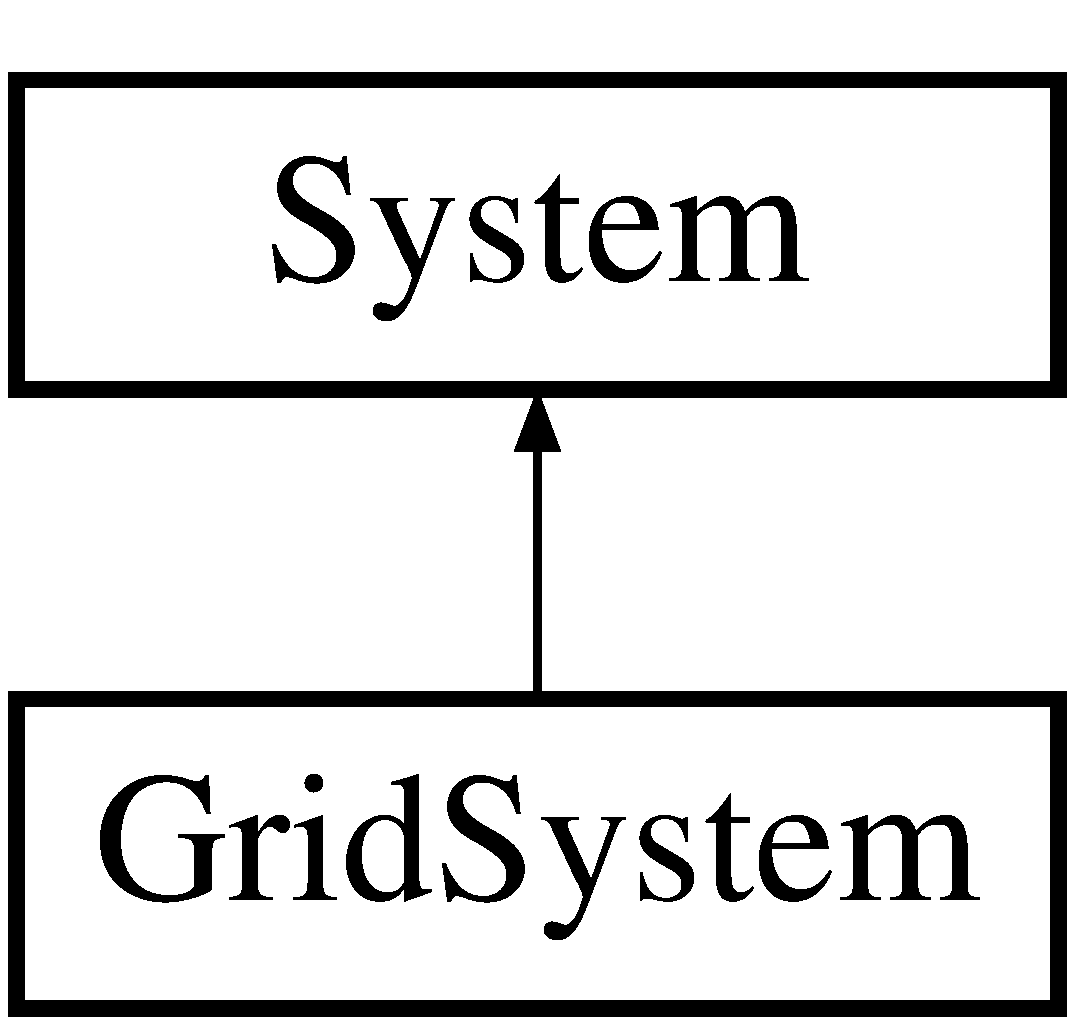
\includegraphics[height=2.000000cm]{class_grid_system}
\end{center}
\end{figure}
\subsection*{Public Member Functions}
\begin{DoxyCompactItemize}
\item 
\hyperlink{class_grid_system_ad868e83a3ef915ba1c1e7d04d5deb8b9}{Grid\+System} (\hyperlink{class_entity_system}{Entity\+System} \&, Ogre\+::\+Scene\+Manager \&)
\begin{DoxyCompactList}\small\item\em Constructor. \end{DoxyCompactList}\item 
\hyperlink{class_grid_system_a7d1f6270ebd9fc98d2647e879b71125c}{$\sim$\+Grid\+System} ()=default
\begin{DoxyCompactList}\small\item\em Destructor. \end{DoxyCompactList}\item 
void \hyperlink{class_grid_system_a4a63a4d431ce96dadcbb1603a88bf71b}{update} (tdt\+::real) override
\begin{DoxyCompactList}\small\item\em Checks if any nodes were freed or unfreed and if so, corrects any path that had those nodes in it. \end{DoxyCompactList}\item 
void \hyperlink{class_grid_system_aa49a509dc8a59c53f9cc043892842f90}{create\+\_\+graphics} ()
\begin{DoxyCompactList}\small\item\em Creates and initializes Ogre models for nodes, which allows the developer to display them for testing purposes. \end{DoxyCompactList}\item 
void \hyperlink{class_grid_system_acce98eec795358ddf184934db96c04b2}{delete\+\_\+graphics} ()
\begin{DoxyCompactList}\small\item\em Deletes Ogre models of all nodes. \end{DoxyCompactList}\item 
void \hyperlink{class_grid_system_aae965431008678ee374fe67e0bc90734}{set\+\_\+visible} (bool)
\begin{DoxyCompactList}\small\item\em Changes the visibility status of the nodes if the graphics have been created already, does nothing otherwise. \end{DoxyCompactList}\item 
bool \hyperlink{class_grid_system_ae2e8bd4a285fe72fe10c93a60f5bfa88}{is\+\_\+visible} () const 
\begin{DoxyCompactList}\small\item\em Returns true if the the grid models are visible, false otherwise. \end{DoxyCompactList}\item 
void \hyperlink{class_grid_system_a7d222c190fbb33b534459664c5c20e97}{place\+\_\+structure} (tdt\+::uint, tdt\+::uint, tdt\+::uint)
\begin{DoxyCompactList}\small\item\em Places a structure (building, wall...) by changing the nodes it is placed on to not free, managing residences etc. \end{DoxyCompactList}\end{DoxyCompactItemize}
\subsection*{Private Member Functions}
\begin{DoxyCompactItemize}
\item 
void \hyperlink{class_grid_system_af9dce4987f42acc6797026fd9393f3c3}{update\+\_\+neighbours\+\_\+} (tdt\+::uint)
\begin{DoxyCompactList}\small\item\em Updates the nodes resident\textquotesingle{}s alignment (if possible) when it\textquotesingle{}s neighbour was freed/unfreed. \end{DoxyCompactList}\end{DoxyCompactItemize}
\subsection*{Private Attributes}
\begin{DoxyCompactItemize}
\item 
\hyperlink{class_entity_system}{Entity\+System} \& \hyperlink{class_grid_system_a76b61fafd9e04fe8a6b67c327d2eeac5}{entities\+\_\+}
\begin{DoxyCompactList}\small\item\em Reference to the game\textquotesingle{}s entity system. \end{DoxyCompactList}\item 
Ogre\+::\+Scene\+Manager \& \hyperlink{class_grid_system_a01626368dc7fde9dfc4b7961aa93cfe9}{scene\+\_\+mgr\+\_\+}
\begin{DoxyCompactList}\small\item\em Reference to the game\textquotesingle{}s main scene manager (used for graphics creation). \end{DoxyCompactList}\item 
bool \hyperlink{class_grid_system_a449d916909013f7d41f81e1ff236d0f6}{graphics\+\_\+loaded\+\_\+}
\begin{DoxyCompactList}\small\item\em Determine if the graphics have been loaded and if the graph is visible (which is only relevant if the former is true). \end{DoxyCompactList}\item 
bool {\bfseries graph\+\_\+visible\+\_\+}\hypertarget{class_grid_system_aeb08f54fd4ce73243bc7ebe0b226147a}{}\label{class_grid_system_aeb08f54fd4ce73243bc7ebe0b226147a}

\end{DoxyCompactItemize}


\subsection{Detailed Description}
Represents the pathfinding graph used by the game and provides several methods related to pathfinding that can be used in Lua. 

Definition at line 11 of file Grid\+System.\+hpp.



\subsection{Constructor \& Destructor Documentation}
\index{Grid\+System@{Grid\+System}!Grid\+System@{Grid\+System}}
\index{Grid\+System@{Grid\+System}!Grid\+System@{Grid\+System}}
\subsubsection[{\texorpdfstring{Grid\+System(\+Entity\+System \&, Ogre\+::\+Scene\+Manager \&)}{GridSystem(EntitySystem &, Ogre::SceneManager &)}}]{\setlength{\rightskip}{0pt plus 5cm}Grid\+System\+::\+Grid\+System (
\begin{DoxyParamCaption}
\item[{{\bf Entity\+System} \&}]{ents, }
\item[{Ogre\+::\+Scene\+Manager \&}]{scene}
\end{DoxyParamCaption}
)}\hypertarget{class_grid_system_ad868e83a3ef915ba1c1e7d04d5deb8b9}{}\label{class_grid_system_ad868e83a3ef915ba1c1e7d04d5deb8b9}


Constructor. 


\begin{DoxyParams}{Parameters}
{\em Reference} & to the game\textquotesingle{}s entity system. \\
\hline
{\em Reference} & to the game\textquotesingle{}s main scene manager. \\
\hline
\end{DoxyParams}


Definition at line 12 of file Grid\+System.\+cpp.

\index{Grid\+System@{Grid\+System}!````~Grid\+System@{$\sim$\+Grid\+System}}
\index{````~Grid\+System@{$\sim$\+Grid\+System}!Grid\+System@{Grid\+System}}
\subsubsection[{\texorpdfstring{$\sim$\+Grid\+System()=default}{~GridSystem()=default}}]{\setlength{\rightskip}{0pt plus 5cm}Grid\+System\+::$\sim$\+Grid\+System (
\begin{DoxyParamCaption}
{}
\end{DoxyParamCaption}
)\hspace{0.3cm}{\ttfamily [default]}}\hypertarget{class_grid_system_a7d1f6270ebd9fc98d2647e879b71125c}{}\label{class_grid_system_a7d1f6270ebd9fc98d2647e879b71125c}


Destructor. 



\subsection{Member Function Documentation}
\index{Grid\+System@{Grid\+System}!create\+\_\+graphics@{create\+\_\+graphics}}
\index{create\+\_\+graphics@{create\+\_\+graphics}!Grid\+System@{Grid\+System}}
\subsubsection[{\texorpdfstring{create\+\_\+graphics()}{create_graphics()}}]{\setlength{\rightskip}{0pt plus 5cm}void Grid\+System\+::create\+\_\+graphics (
\begin{DoxyParamCaption}
{}
\end{DoxyParamCaption}
)}\hypertarget{class_grid_system_aa49a509dc8a59c53f9cc043892842f90}{}\label{class_grid_system_aa49a509dc8a59c53f9cc043892842f90}


Creates and initializes Ogre models for nodes, which allows the developer to display them for testing purposes. 



Definition at line 80 of file Grid\+System.\+cpp.

\index{Grid\+System@{Grid\+System}!delete\+\_\+graphics@{delete\+\_\+graphics}}
\index{delete\+\_\+graphics@{delete\+\_\+graphics}!Grid\+System@{Grid\+System}}
\subsubsection[{\texorpdfstring{delete\+\_\+graphics()}{delete_graphics()}}]{\setlength{\rightskip}{0pt plus 5cm}void Grid\+System\+::delete\+\_\+graphics (
\begin{DoxyParamCaption}
{}
\end{DoxyParamCaption}
)}\hypertarget{class_grid_system_acce98eec795358ddf184934db96c04b2}{}\label{class_grid_system_acce98eec795358ddf184934db96c04b2}


Deletes Ogre models of all nodes. 



Definition at line 106 of file Grid\+System.\+cpp.

\index{Grid\+System@{Grid\+System}!is\+\_\+visible@{is\+\_\+visible}}
\index{is\+\_\+visible@{is\+\_\+visible}!Grid\+System@{Grid\+System}}
\subsubsection[{\texorpdfstring{is\+\_\+visible() const }{is_visible() const }}]{\setlength{\rightskip}{0pt plus 5cm}bool Grid\+System\+::is\+\_\+visible (
\begin{DoxyParamCaption}
{}
\end{DoxyParamCaption}
) const}\hypertarget{class_grid_system_ae2e8bd4a285fe72fe10c93a60f5bfa88}{}\label{class_grid_system_ae2e8bd4a285fe72fe10c93a60f5bfa88}


Returns true if the the grid models are visible, false otherwise. 



Definition at line 130 of file Grid\+System.\+cpp.

\index{Grid\+System@{Grid\+System}!place\+\_\+structure@{place\+\_\+structure}}
\index{place\+\_\+structure@{place\+\_\+structure}!Grid\+System@{Grid\+System}}
\subsubsection[{\texorpdfstring{place\+\_\+structure(tdt\+::uint, tdt\+::uint, tdt\+::uint)}{place_structure(tdt::uint, tdt::uint, tdt::uint)}}]{\setlength{\rightskip}{0pt plus 5cm}void Grid\+System\+::place\+\_\+structure (
\begin{DoxyParamCaption}
\item[{tdt\+::uint}]{ent\+\_\+id, }
\item[{tdt\+::uint}]{node\+\_\+id, }
\item[{tdt\+::uint}]{radius}
\end{DoxyParamCaption}
)}\hypertarget{class_grid_system_a7d222c190fbb33b534459664c5c20e97}{}\label{class_grid_system_a7d222c190fbb33b534459664c5c20e97}


Places a structure (building, wall...) by changing the nodes it is placed on to not free, managing residences etc. 


\begin{DoxyParams}{Parameters}
{\em ID} & of the structure. \\
\hline
{\em ID} & of the central node. \\
\hline
{\em Radius} & of the structure. \\
\hline
\end{DoxyParams}


Definition at line 138 of file Grid\+System.\+cpp.

\index{Grid\+System@{Grid\+System}!set\+\_\+visible@{set\+\_\+visible}}
\index{set\+\_\+visible@{set\+\_\+visible}!Grid\+System@{Grid\+System}}
\subsubsection[{\texorpdfstring{set\+\_\+visible(bool)}{set_visible(bool)}}]{\setlength{\rightskip}{0pt plus 5cm}void Grid\+System\+::set\+\_\+visible (
\begin{DoxyParamCaption}
\item[{bool}]{on\+\_\+off}
\end{DoxyParamCaption}
)}\hypertarget{class_grid_system_aae965431008678ee374fe67e0bc90734}{}\label{class_grid_system_aae965431008678ee374fe67e0bc90734}


Changes the visibility status of the nodes if the graphics have been created already, does nothing otherwise. 


\begin{DoxyParams}{Parameters}
{\em The} & new visibility status. \\
\hline
\end{DoxyParams}


Definition at line 114 of file Grid\+System.\+cpp.

\index{Grid\+System@{Grid\+System}!update@{update}}
\index{update@{update}!Grid\+System@{Grid\+System}}
\subsubsection[{\texorpdfstring{update(tdt\+::real) override}{update(tdt::real) override}}]{\setlength{\rightskip}{0pt plus 5cm}void Grid\+System\+::update (
\begin{DoxyParamCaption}
\item[{tdt\+::real}]{}
\end{DoxyParamCaption}
)\hspace{0.3cm}{\ttfamily [override]}, {\ttfamily [virtual]}}\hypertarget{class_grid_system_a4a63a4d431ce96dadcbb1603a88bf71b}{}\label{class_grid_system_a4a63a4d431ce96dadcbb1603a88bf71b}


Checks if any nodes were freed or unfreed and if so, corrects any path that had those nodes in it. 


\begin{DoxyParams}{Parameters}
{\em Time} & since the last frame. \\
\hline
\end{DoxyParams}


Implements \hyperlink{class_system_a6d54c9bd38eb43d620a1451cb0925472}{System}.



Definition at line 17 of file Grid\+System.\+cpp.

\index{Grid\+System@{Grid\+System}!update\+\_\+neighbours\+\_\+@{update\+\_\+neighbours\+\_\+}}
\index{update\+\_\+neighbours\+\_\+@{update\+\_\+neighbours\+\_\+}!Grid\+System@{Grid\+System}}
\subsubsection[{\texorpdfstring{update\+\_\+neighbours\+\_\+(tdt\+::uint)}{update_neighbours_(tdt::uint)}}]{\setlength{\rightskip}{0pt plus 5cm}void Grid\+System\+::update\+\_\+neighbours\+\_\+ (
\begin{DoxyParamCaption}
\item[{tdt\+::uint}]{id}
\end{DoxyParamCaption}
)\hspace{0.3cm}{\ttfamily [private]}}\hypertarget{class_grid_system_af9dce4987f42acc6797026fd9393f3c3}{}\label{class_grid_system_af9dce4987f42acc6797026fd9393f3c3}


Updates the nodes resident\textquotesingle{}s alignment (if possible) when it\textquotesingle{}s neighbour was freed/unfreed. 


\begin{DoxyParams}{Parameters}
{\em ID} & of the node. \\
\hline
\end{DoxyParams}


Definition at line 168 of file Grid\+System.\+cpp.



\subsection{Member Data Documentation}
\index{Grid\+System@{Grid\+System}!entities\+\_\+@{entities\+\_\+}}
\index{entities\+\_\+@{entities\+\_\+}!Grid\+System@{Grid\+System}}
\subsubsection[{\texorpdfstring{entities\+\_\+}{entities_}}]{\setlength{\rightskip}{0pt plus 5cm}{\bf Entity\+System}\& Grid\+System\+::entities\+\_\+\hspace{0.3cm}{\ttfamily [private]}}\hypertarget{class_grid_system_a76b61fafd9e04fe8a6b67c327d2eeac5}{}\label{class_grid_system_a76b61fafd9e04fe8a6b67c327d2eeac5}


Reference to the game\textquotesingle{}s entity system. 



Definition at line 76 of file Grid\+System.\+hpp.

\index{Grid\+System@{Grid\+System}!graphics\+\_\+loaded\+\_\+@{graphics\+\_\+loaded\+\_\+}}
\index{graphics\+\_\+loaded\+\_\+@{graphics\+\_\+loaded\+\_\+}!Grid\+System@{Grid\+System}}
\subsubsection[{\texorpdfstring{graphics\+\_\+loaded\+\_\+}{graphics_loaded_}}]{\setlength{\rightskip}{0pt plus 5cm}bool Grid\+System\+::graphics\+\_\+loaded\+\_\+\hspace{0.3cm}{\ttfamily [private]}}\hypertarget{class_grid_system_a449d916909013f7d41f81e1ff236d0f6}{}\label{class_grid_system_a449d916909013f7d41f81e1ff236d0f6}


Determine if the graphics have been loaded and if the graph is visible (which is only relevant if the former is true). 



Definition at line 88 of file Grid\+System.\+hpp.

\index{Grid\+System@{Grid\+System}!scene\+\_\+mgr\+\_\+@{scene\+\_\+mgr\+\_\+}}
\index{scene\+\_\+mgr\+\_\+@{scene\+\_\+mgr\+\_\+}!Grid\+System@{Grid\+System}}
\subsubsection[{\texorpdfstring{scene\+\_\+mgr\+\_\+}{scene_mgr_}}]{\setlength{\rightskip}{0pt plus 5cm}Ogre\+::\+Scene\+Manager\& Grid\+System\+::scene\+\_\+mgr\+\_\+\hspace{0.3cm}{\ttfamily [private]}}\hypertarget{class_grid_system_a01626368dc7fde9dfc4b7961aa93cfe9}{}\label{class_grid_system_a01626368dc7fde9dfc4b7961aa93cfe9}


Reference to the game\textquotesingle{}s main scene manager (used for graphics creation). 



Definition at line 81 of file Grid\+System.\+hpp.



The documentation for this class was generated from the following files\+:\begin{DoxyCompactItemize}
\item 
systems/Grid\+System.\+hpp\item 
systems/Grid\+System.\+cpp\end{DoxyCompactItemize}

\hypertarget{class_g_u_i}{}\section{G\+UI Class Reference}
\label{class_g_u_i}\index{G\+UI@{G\+UI}}


Represents the game\textquotesingle{}s main graphical user interface (i.\+e.  




{\ttfamily \#include $<$G\+U\+I.\+hpp$>$}

\subsection*{Public Member Functions}
\begin{DoxyCompactItemize}
\item 
\hyperlink{class_g_u_i_ac9cae2328dcb5d83bdfaeca49a2eb695}{$\sim$\+G\+UI} ()
\begin{DoxyCompactList}\small\item\em Destructor. \end{DoxyCompactList}\item 
void \hyperlink{class_g_u_i_a91b0fc72a458e688947da1c86e859750}{init} (\hyperlink{class_game}{Game} $\ast$)
\begin{DoxyCompactList}\small\item\em Initializes the selection by loading the layout and registering all event handlers. \end{DoxyCompactList}\item 
void \hyperlink{class_g_u_i_a37c94218f5c1d9d9b955ee7796ba9247}{set\+\_\+visible} (bool)
\begin{DoxyCompactList}\small\item\em Set\textquotesingle{}s the \hyperlink{class_g_u_i}{G\+UI}\textquotesingle{}s visibility status. \end{DoxyCompactList}\item 
bool \hyperlink{class_g_u_i_af2fb755008d9734fef2c0d4f94ad5bab}{is\+\_\+visible} () const 
\begin{DoxyCompactList}\small\item\em Returns true if the entire \hyperlink{class_g_u_i}{G\+UI} is visible, false otherwise. \end{DoxyCompactList}\item 
void \hyperlink{class_g_u_i_a56664bc17967fdb694c5876a23229830}{set\+\_\+visible} (const std\+::string \&, bool)
\begin{DoxyCompactList}\small\item\em Set\textquotesingle{}s the visibility status of a particular window. \end{DoxyCompactList}\item 
bool \hyperlink{class_g_u_i_ae990bd08d2db58fcba2a15e261e618f1}{is\+\_\+visible} (const std\+::string \&) const 
\begin{DoxyCompactList}\small\item\em Returns the visibility status of a particular window. \end{DoxyCompactList}\item 
void \hyperlink{class_g_u_i_a6bf316dac4af6edbc03e9e6f6a1842a7}{show\+\_\+load\+\_\+save\+\_\+dialog} (const std\+::string \&)
\begin{DoxyCompactList}\small\item\em Shows the load/save dialog window. \end{DoxyCompactList}\item 
C\+E\+G\+U\+I\+::\+Window $\ast$ \hyperlink{class_g_u_i_a825a335740e695b10d60e0c96ffeb0b5}{get\+\_\+window} ()
\begin{DoxyCompactList}\small\item\em Returns a pointer to the root window. \end{DoxyCompactList}\item 
C\+E\+G\+U\+I\+::\+Window $\ast$ \hyperlink{class_g_u_i_a392281fef48b437e8d3b4a5fbab09191}{get\+\_\+window} (const std\+::string \&)
\begin{DoxyCompactList}\small\item\em Returns a pointer to a given subwindow of the root window. \end{DoxyCompactList}\item 
\hyperlink{class_console}{Console} \& \hyperlink{class_g_u_i_ae407027b2e7e81f8132ee7dd5252c456}{get\+\_\+console} ()
\begin{DoxyCompactList}\small\item\em Returns a reference to the game\textquotesingle{}s dev console. \end{DoxyCompactList}\item 
\hyperlink{class_entity_tracker}{Entity\+Tracker} \& \hyperlink{class_g_u_i_ab197361fb542ae6f1761be27346ec6bd}{get\+\_\+tracker} ()
\begin{DoxyCompactList}\small\item\em Returns a reference to the entity tracker. \end{DoxyCompactList}\item 
\hyperlink{class_game_log}{Game\+Log} \& \hyperlink{class_g_u_i_ac5d029ac1d5be5f405d0bb9b4beaadeb}{get\+\_\+log} ()
\begin{DoxyCompactList}\small\item\em Returns a reference to the game\textquotesingle{}s log. \end{DoxyCompactList}\item 
\hyperlink{class_builder_window}{Builder\+Window} \& \hyperlink{class_g_u_i_a3533e8d1c67c8cd1643be0b6d640e489}{get\+\_\+builder} ()
\begin{DoxyCompactList}\small\item\em Returns a reference to the builder window. \end{DoxyCompactList}\item 
\hyperlink{class_top_bar}{Top\+Bar} \& \hyperlink{class_g_u_i_a57b2102ded949460275f6c06a73ef472}{get\+\_\+top\+\_\+bar} ()
\begin{DoxyCompactList}\small\item\em Returns a reference to the top bar. \end{DoxyCompactList}\item 
\hyperlink{class_research_window}{Research\+Window} \& \hyperlink{class_g_u_i_a8f8dae1e40b3f25c179cd088631e9e24}{get\+\_\+research} ()
\begin{DoxyCompactList}\small\item\em Returns a reference to the research window. \end{DoxyCompactList}\item 
\hyperlink{class_spell_casting_window}{Spell\+Casting\+Window} \& \hyperlink{class_g_u_i_ad68dfd48d702edbc8eae79b02ef694db}{get\+\_\+spell\+\_\+casting} ()
\begin{DoxyCompactList}\small\item\em Returns a reference to the spell casting window. \end{DoxyCompactList}\item 
\hyperlink{class_message_to_player_window}{Message\+To\+Player\+Window} \& \hyperlink{class_g_u_i_af7f76a45f16144b8217938de6facb97d}{get\+\_\+message} ()
\begin{DoxyCompactList}\small\item\em Returns a reference to the message to player window. \end{DoxyCompactList}\item 
\hyperlink{class_options_window}{Options\+Window} \& \hyperlink{class_g_u_i_adf043e9ed8ec60a8ac7f981dbd3d7933}{get\+\_\+options} ()
\begin{DoxyCompactList}\small\item\em Returns a reference to the options window. \end{DoxyCompactList}\item 
bool \hyperlink{class_g_u_i_a8c3e6a481d74bb0673389b596989047c}{escape\+\_\+pressed} ()
\begin{DoxyCompactList}\small\item\em Notifies the \hyperlink{class_g_u_i}{G\+UI} that the escape key was pressed so that it can close windows if needed. \end{DoxyCompactList}\item 
void \hyperlink{class_g_u_i_ae841ba53ef5f7152fa900c682edc9788}{set\+\_\+curr\+\_\+tool\+\_\+visible} (bool)
\begin{DoxyCompactList}\small\item\em Sets the visibility status of the current tool window. \end{DoxyCompactList}\item 
void \hyperlink{class_g_u_i_ad27594472b3c4625d5cf1ca24b31d1a4}{set\+\_\+curr\+\_\+tool} (const std\+::string \&)
\begin{DoxyCompactList}\small\item\em Sets the current tool window. \end{DoxyCompactList}\item 
const std\+::string \& \hyperlink{class_g_u_i_a1640c56f8c04cea1df046220781f9d22}{get\+\_\+curr\+\_\+tool} ()
\begin{DoxyCompactList}\small\item\em Returns the name of the current tool window. \end{DoxyCompactList}\item 
\hyperlink{class_g_u_i_a0b8d80c1dc4e62859e0f0b80d6175205}{G\+UI} (const \hyperlink{class_g_u_i}{G\+UI} \&)=delete
\item 
{\bfseries G\+UI} (\hyperlink{class_g_u_i}{G\+UI} \&\&)=delete\hypertarget{class_g_u_i_a9bbaf9f1720fecb1f260f10473fe1323}{}\label{class_g_u_i_a9bbaf9f1720fecb1f260f10473fe1323}

\item 
\hyperlink{class_g_u_i}{G\+UI} \& {\bfseries operator=} (const \hyperlink{class_g_u_i}{G\+UI} \&)=delete\hypertarget{class_g_u_i_ae3f7d63739574619a294f606696f50db}{}\label{class_g_u_i_ae3f7d63739574619a294f606696f50db}

\item 
\hyperlink{class_g_u_i}{G\+UI} \& {\bfseries operator=} (\hyperlink{class_g_u_i}{G\+UI} \&\&)=delete\hypertarget{class_g_u_i_a3553773dac200692ecabcfdeb3ae2f51}{}\label{class_g_u_i_a3553773dac200692ecabcfdeb3ae2f51}

\end{DoxyCompactItemize}
\subsection*{Static Public Member Functions}
\begin{DoxyCompactItemize}
\item 
static \hyperlink{class_g_u_i}{G\+UI} \& \hyperlink{class_g_u_i_a169694dda858ea12986f00ee32ac7add}{instance} ()
\begin{DoxyCompactList}\small\item\em Returns the singleton instance. \end{DoxyCompactList}\end{DoxyCompactItemize}
\subsection*{Private Member Functions}
\begin{DoxyCompactItemize}
\item 
\hyperlink{class_g_u_i_a8cbb3140b7d3c9d8e942d6ce6b60a0e8}{G\+UI} ()
\begin{DoxyCompactList}\small\item\em Constructor, private because of the singleton pattern. \end{DoxyCompactList}\item 
void \hyperlink{class_g_u_i_a457e1e62289a5da4eef425cb526d0e5b}{list\+\_\+directory} (const std\+::string \&, C\+E\+G\+U\+I\+::\+Listbox \&, bool=false)
\begin{DoxyCompactList}\small\item\em Fills a given list box with the names of all files in a given directory. \end{DoxyCompactList}\end{DoxyCompactItemize}
\subsection*{Private Attributes}
\begin{DoxyCompactItemize}
\item 
C\+E\+G\+U\+I\+::\+Window $\ast$ \hyperlink{class_g_u_i_a1216023a7675f2d5c6f3a33d6f2b9eca}{window\+\_\+}
\begin{DoxyCompactList}\small\item\em Pointer to the root window of the layout. \end{DoxyCompactList}\item 
std\+::string \hyperlink{class_g_u_i_a8ee9091320921548eca2305ec60d5182}{curr\+\_\+tool\+\_\+}
\begin{DoxyCompactList}\small\item\em Name of the current tool in the tools subwindow. \end{DoxyCompactList}\item 
\hyperlink{class_game}{Game} $\ast$ \hyperlink{class_g_u_i_a8af61511961fc5de258e1fd8e03eeed4}{game\+\_\+}
\begin{DoxyCompactList}\small\item\em Pointer to the game instance used by button event handlers. \end{DoxyCompactList}\item 
\hyperlink{class_entity_tracker}{Entity\+Tracker} \hyperlink{class_g_u_i_a90c490c7ff853531ac635f08408d59bf}{tracker\+\_\+}
\begin{DoxyCompactList}\small\item\em ID of the entity that is currently tracked by the entity viewer. \end{DoxyCompactList}\item 
\hyperlink{class_console}{Console} \hyperlink{class_g_u_i_aa16bd75eb28be973d2df6480cc65c68b}{console\+\_\+}
\begin{DoxyCompactList}\small\item\em \hyperlink{class_game}{Game}\textquotesingle{}s developer console. \end{DoxyCompactList}\item 
\hyperlink{class_game_log}{Game\+Log} \hyperlink{class_g_u_i_a2290d6a10a481beaa55dd93913ceadaf}{log\+\_\+}
\begin{DoxyCompactList}\small\item\em \hyperlink{class_game}{Game}\textquotesingle{}s log, used to show messages to the player. \end{DoxyCompactList}\item 
\hyperlink{class_builder_window}{Builder\+Window} \hyperlink{class_g_u_i_a0384e5c8eeb11e4181ca31e621a897cb}{builder\+\_\+}
\begin{DoxyCompactList}\small\item\em Allows the player to place buildings. \end{DoxyCompactList}\item 
\hyperlink{class_top_bar}{Top\+Bar} \hyperlink{class_g_u_i_a6de1adcb5f3b762f3f99e7b37db61740}{top\+\_\+bar\+\_\+}
\begin{DoxyCompactList}\small\item\em Shows game info at the top of the screen. \end{DoxyCompactList}\item 
\hyperlink{class_research_window}{Research\+Window} \hyperlink{class_g_u_i_a37611f1e119a7c0b0d8d9682ac8a9432}{research\+\_\+}
\begin{DoxyCompactList}\small\item\em \hyperlink{class_game}{Game}\textquotesingle{}s research window that allows the player to buy buildings, units and spells. \end{DoxyCompactList}\item 
\hyperlink{class_spell_casting_window}{Spell\+Casting\+Window} \hyperlink{class_g_u_i_a434c351b8b781d7bf19dfbae30bc7d73}{spell\+\_\+casting\+\_\+}
\begin{DoxyCompactList}\small\item\em Allows the player to cast spells. \end{DoxyCompactList}\item 
C\+E\+G\+U\+I\+::\+Window $\ast$ \hyperlink{class_g_u_i_aa9a52eb5090edfa1e62773be5dd03da3}{menu\+\_\+}
\begin{DoxyCompactList}\small\item\em Allows easier access to the menu subwindow. \end{DoxyCompactList}\item 
\hyperlink{class_message_to_player_window}{Message\+To\+Player\+Window} \hyperlink{class_g_u_i_a447ea4f3f0b635717a3a88317f534825}{message\+\_\+}
\begin{DoxyCompactList}\small\item\em Allows the game to show a message to the player with any of the following buttons\+: OK, Y\+ES, NO. \end{DoxyCompactList}\item 
\hyperlink{class_options_window}{Options\+Window} \hyperlink{class_g_u_i_ac08ccbb1a55bae003d956ff299db3d91}{options\+\_\+}
\begin{DoxyCompactList}\small\item\em Allows to change the resolution, window mode and key bindings. \end{DoxyCompactList}\end{DoxyCompactItemize}
\subsection*{Friends}
\begin{DoxyCompactItemize}
\item 
class {\bfseries Options\+Window}\hypertarget{class_g_u_i_a720341fa2258af1b64cf4f505d8226a1}{}\label{class_g_u_i_a720341fa2258af1b64cf4f505d8226a1}

\item 
void {\bfseries action\+::\+Q\+U\+I\+C\+K\+\_\+\+L\+O\+AD} ()\hypertarget{class_g_u_i_afcaa4fe027cc52b7f11e80caedfb2f96}{}\label{class_g_u_i_afcaa4fe027cc52b7f11e80caedfb2f96}

\item 
void {\bfseries action\+::\+Q\+U\+I\+C\+K\+\_\+\+S\+A\+VE} ()\hypertarget{class_g_u_i_ac91f206467cf888fb767b7d7d03b92ba}{}\label{class_g_u_i_ac91f206467cf888fb767b7d7d03b92ba}

\item 
void {\bfseries action\+::\+R\+E\+S\+E\+T\+\_\+\+C\+A\+M\+E\+RA} ()\hypertarget{class_g_u_i_a94cac4560c54379f3013e5074558f322}{}\label{class_g_u_i_a94cac4560c54379f3013e5074558f322}

\end{DoxyCompactItemize}


\subsection{Detailed Description}
Represents the game\textquotesingle{}s main graphical user interface (i.\+e. 

any windows except for the development ones like the console or entity creator). 

Definition at line 26 of file G\+U\+I.\+hpp.



\subsection{Constructor \& Destructor Documentation}
\index{G\+UI@{G\+UI}!````~G\+UI@{$\sim$\+G\+UI}}
\index{````~G\+UI@{$\sim$\+G\+UI}!G\+UI@{G\+UI}}
\subsubsection[{\texorpdfstring{$\sim$\+G\+U\+I()}{~GUI()}}]{\setlength{\rightskip}{0pt plus 5cm}G\+U\+I\+::$\sim$\+G\+UI (
\begin{DoxyParamCaption}
{}
\end{DoxyParamCaption}
)\hspace{0.3cm}{\ttfamily [inline]}}\hypertarget{class_g_u_i_ac9cae2328dcb5d83bdfaeca49a2eb695}{}\label{class_g_u_i_ac9cae2328dcb5d83bdfaeca49a2eb695}


Destructor. 



Definition at line 36 of file G\+U\+I.\+hpp.

\index{G\+UI@{G\+UI}!G\+UI@{G\+UI}}
\index{G\+UI@{G\+UI}!G\+UI@{G\+UI}}
\subsubsection[{\texorpdfstring{G\+U\+I(const G\+U\+I \&)=delete}{GUI(const GUI &)=delete}}]{\setlength{\rightskip}{0pt plus 5cm}G\+U\+I\+::\+G\+UI (
\begin{DoxyParamCaption}
\item[{const {\bf G\+UI} \&}]{}
\end{DoxyParamCaption}
)\hspace{0.3cm}{\ttfamily [delete]}}\hypertarget{class_g_u_i_a0b8d80c1dc4e62859e0f0b80d6175205}{}\label{class_g_u_i_a0b8d80c1dc4e62859e0f0b80d6175205}
\begin{DoxyNote}{Note}
Since V\+S2015 seems to have some problems with C++ standard (generates default copy/move constructors and operators even if default constructor is created), these constructors/operators are explicitly deleted. 
\end{DoxyNote}
\index{G\+UI@{G\+UI}!G\+UI@{G\+UI}}
\index{G\+UI@{G\+UI}!G\+UI@{G\+UI}}
\subsubsection[{\texorpdfstring{G\+U\+I()}{GUI()}}]{\setlength{\rightskip}{0pt plus 5cm}G\+U\+I\+::\+G\+UI (
\begin{DoxyParamCaption}
{}
\end{DoxyParamCaption}
)\hspace{0.3cm}{\ttfamily [private]}}\hypertarget{class_g_u_i_a8cbb3140b7d3c9d8e942d6ce6b60a0e8}{}\label{class_g_u_i_a8cbb3140b7d3c9d8e942d6ce6b60a0e8}


Constructor, private because of the singleton pattern. 



Definition at line 7 of file G\+U\+I.\+cpp.



\subsection{Member Function Documentation}
\index{G\+UI@{G\+UI}!escape\+\_\+pressed@{escape\+\_\+pressed}}
\index{escape\+\_\+pressed@{escape\+\_\+pressed}!G\+UI@{G\+UI}}
\subsubsection[{\texorpdfstring{escape\+\_\+pressed()}{escape_pressed()}}]{\setlength{\rightskip}{0pt plus 5cm}bool G\+U\+I\+::escape\+\_\+pressed (
\begin{DoxyParamCaption}
{}
\end{DoxyParamCaption}
)}\hypertarget{class_g_u_i_a8c3e6a481d74bb0673389b596989047c}{}\label{class_g_u_i_a8c3e6a481d74bb0673389b596989047c}


Notifies the \hyperlink{class_g_u_i}{G\+UI} that the escape key was pressed so that it can close windows if needed. 

Returns true if anything has been closed, false otherwise. \begin{DoxyNote}{Note}
C\+E\+G\+UI event system does not seem to work properly \+:/ 
\end{DoxyNote}
This will allow the return from the main menu (which does not happend when a submenu window is visible).

Definition at line 414 of file G\+U\+I.\+cpp.

\index{G\+UI@{G\+UI}!get\+\_\+builder@{get\+\_\+builder}}
\index{get\+\_\+builder@{get\+\_\+builder}!G\+UI@{G\+UI}}
\subsubsection[{\texorpdfstring{get\+\_\+builder()}{get_builder()}}]{\setlength{\rightskip}{0pt plus 5cm}{\bf Builder\+Window} \& G\+U\+I\+::get\+\_\+builder (
\begin{DoxyParamCaption}
{}
\end{DoxyParamCaption}
)}\hypertarget{class_g_u_i_a3533e8d1c67c8cd1643be0b6d640e489}{}\label{class_g_u_i_a3533e8d1c67c8cd1643be0b6d640e489}


Returns a reference to the builder window. 



Definition at line 384 of file G\+U\+I.\+cpp.

\index{G\+UI@{G\+UI}!get\+\_\+console@{get\+\_\+console}}
\index{get\+\_\+console@{get\+\_\+console}!G\+UI@{G\+UI}}
\subsubsection[{\texorpdfstring{get\+\_\+console()}{get_console()}}]{\setlength{\rightskip}{0pt plus 5cm}{\bf Console} \& G\+U\+I\+::get\+\_\+console (
\begin{DoxyParamCaption}
{}
\end{DoxyParamCaption}
)}\hypertarget{class_g_u_i_ae407027b2e7e81f8132ee7dd5252c456}{}\label{class_g_u_i_ae407027b2e7e81f8132ee7dd5252c456}


Returns a reference to the game\textquotesingle{}s dev console. 



Definition at line 369 of file G\+U\+I.\+cpp.

\index{G\+UI@{G\+UI}!get\+\_\+curr\+\_\+tool@{get\+\_\+curr\+\_\+tool}}
\index{get\+\_\+curr\+\_\+tool@{get\+\_\+curr\+\_\+tool}!G\+UI@{G\+UI}}
\subsubsection[{\texorpdfstring{get\+\_\+curr\+\_\+tool()}{get_curr_tool()}}]{\setlength{\rightskip}{0pt plus 5cm}const std\+::string \& G\+U\+I\+::get\+\_\+curr\+\_\+tool (
\begin{DoxyParamCaption}
{}
\end{DoxyParamCaption}
)}\hypertarget{class_g_u_i_a1640c56f8c04cea1df046220781f9d22}{}\label{class_g_u_i_a1640c56f8c04cea1df046220781f9d22}


Returns the name of the current tool window. 



Definition at line 465 of file G\+U\+I.\+cpp.

\index{G\+UI@{G\+UI}!get\+\_\+log@{get\+\_\+log}}
\index{get\+\_\+log@{get\+\_\+log}!G\+UI@{G\+UI}}
\subsubsection[{\texorpdfstring{get\+\_\+log()}{get_log()}}]{\setlength{\rightskip}{0pt plus 5cm}{\bf Game\+Log} \& G\+U\+I\+::get\+\_\+log (
\begin{DoxyParamCaption}
{}
\end{DoxyParamCaption}
)}\hypertarget{class_g_u_i_ac5d029ac1d5be5f405d0bb9b4beaadeb}{}\label{class_g_u_i_ac5d029ac1d5be5f405d0bb9b4beaadeb}


Returns a reference to the game\textquotesingle{}s log. 



Definition at line 379 of file G\+U\+I.\+cpp.

\index{G\+UI@{G\+UI}!get\+\_\+message@{get\+\_\+message}}
\index{get\+\_\+message@{get\+\_\+message}!G\+UI@{G\+UI}}
\subsubsection[{\texorpdfstring{get\+\_\+message()}{get_message()}}]{\setlength{\rightskip}{0pt plus 5cm}{\bf Message\+To\+Player\+Window} \& G\+U\+I\+::get\+\_\+message (
\begin{DoxyParamCaption}
{}
\end{DoxyParamCaption}
)}\hypertarget{class_g_u_i_af7f76a45f16144b8217938de6facb97d}{}\label{class_g_u_i_af7f76a45f16144b8217938de6facb97d}


Returns a reference to the message to player window. 



Definition at line 404 of file G\+U\+I.\+cpp.

\index{G\+UI@{G\+UI}!get\+\_\+options@{get\+\_\+options}}
\index{get\+\_\+options@{get\+\_\+options}!G\+UI@{G\+UI}}
\subsubsection[{\texorpdfstring{get\+\_\+options()}{get_options()}}]{\setlength{\rightskip}{0pt plus 5cm}{\bf Options\+Window} \& G\+U\+I\+::get\+\_\+options (
\begin{DoxyParamCaption}
{}
\end{DoxyParamCaption}
)}\hypertarget{class_g_u_i_adf043e9ed8ec60a8ac7f981dbd3d7933}{}\label{class_g_u_i_adf043e9ed8ec60a8ac7f981dbd3d7933}


Returns a reference to the options window. 



Definition at line 409 of file G\+U\+I.\+cpp.

\index{G\+UI@{G\+UI}!get\+\_\+research@{get\+\_\+research}}
\index{get\+\_\+research@{get\+\_\+research}!G\+UI@{G\+UI}}
\subsubsection[{\texorpdfstring{get\+\_\+research()}{get_research()}}]{\setlength{\rightskip}{0pt plus 5cm}{\bf Research\+Window} \& G\+U\+I\+::get\+\_\+research (
\begin{DoxyParamCaption}
{}
\end{DoxyParamCaption}
)}\hypertarget{class_g_u_i_a8f8dae1e40b3f25c179cd088631e9e24}{}\label{class_g_u_i_a8f8dae1e40b3f25c179cd088631e9e24}


Returns a reference to the research window. 



Definition at line 394 of file G\+U\+I.\+cpp.

\index{G\+UI@{G\+UI}!get\+\_\+spell\+\_\+casting@{get\+\_\+spell\+\_\+casting}}
\index{get\+\_\+spell\+\_\+casting@{get\+\_\+spell\+\_\+casting}!G\+UI@{G\+UI}}
\subsubsection[{\texorpdfstring{get\+\_\+spell\+\_\+casting()}{get_spell_casting()}}]{\setlength{\rightskip}{0pt plus 5cm}{\bf Spell\+Casting\+Window} \& G\+U\+I\+::get\+\_\+spell\+\_\+casting (
\begin{DoxyParamCaption}
{}
\end{DoxyParamCaption}
)}\hypertarget{class_g_u_i_ad68dfd48d702edbc8eae79b02ef694db}{}\label{class_g_u_i_ad68dfd48d702edbc8eae79b02ef694db}


Returns a reference to the spell casting window. 



Definition at line 399 of file G\+U\+I.\+cpp.

\index{G\+UI@{G\+UI}!get\+\_\+top\+\_\+bar@{get\+\_\+top\+\_\+bar}}
\index{get\+\_\+top\+\_\+bar@{get\+\_\+top\+\_\+bar}!G\+UI@{G\+UI}}
\subsubsection[{\texorpdfstring{get\+\_\+top\+\_\+bar()}{get_top_bar()}}]{\setlength{\rightskip}{0pt plus 5cm}{\bf Top\+Bar} \& G\+U\+I\+::get\+\_\+top\+\_\+bar (
\begin{DoxyParamCaption}
{}
\end{DoxyParamCaption}
)}\hypertarget{class_g_u_i_a57b2102ded949460275f6c06a73ef472}{}\label{class_g_u_i_a57b2102ded949460275f6c06a73ef472}


Returns a reference to the top bar. 



Definition at line 389 of file G\+U\+I.\+cpp.

\index{G\+UI@{G\+UI}!get\+\_\+tracker@{get\+\_\+tracker}}
\index{get\+\_\+tracker@{get\+\_\+tracker}!G\+UI@{G\+UI}}
\subsubsection[{\texorpdfstring{get\+\_\+tracker()}{get_tracker()}}]{\setlength{\rightskip}{0pt plus 5cm}{\bf Entity\+Tracker} \& G\+U\+I\+::get\+\_\+tracker (
\begin{DoxyParamCaption}
{}
\end{DoxyParamCaption}
)}\hypertarget{class_g_u_i_ab197361fb542ae6f1761be27346ec6bd}{}\label{class_g_u_i_ab197361fb542ae6f1761be27346ec6bd}


Returns a reference to the entity tracker. 



Definition at line 374 of file G\+U\+I.\+cpp.

\index{G\+UI@{G\+UI}!get\+\_\+window@{get\+\_\+window}}
\index{get\+\_\+window@{get\+\_\+window}!G\+UI@{G\+UI}}
\subsubsection[{\texorpdfstring{get\+\_\+window()}{get_window()}}]{\setlength{\rightskip}{0pt plus 5cm}C\+E\+G\+U\+I\+::\+Window $\ast$ G\+U\+I\+::get\+\_\+window (
\begin{DoxyParamCaption}
{}
\end{DoxyParamCaption}
)}\hypertarget{class_g_u_i_a825a335740e695b10d60e0c96ffeb0b5}{}\label{class_g_u_i_a825a335740e695b10d60e0c96ffeb0b5}


Returns a pointer to the root window. 



Definition at line 359 of file G\+U\+I.\+cpp.

\index{G\+UI@{G\+UI}!get\+\_\+window@{get\+\_\+window}}
\index{get\+\_\+window@{get\+\_\+window}!G\+UI@{G\+UI}}
\subsubsection[{\texorpdfstring{get\+\_\+window(const std\+::string \&)}{get_window(const std::string &)}}]{\setlength{\rightskip}{0pt plus 5cm}C\+E\+G\+U\+I\+::\+Window $\ast$ G\+U\+I\+::get\+\_\+window (
\begin{DoxyParamCaption}
\item[{const std\+::string \&}]{name}
\end{DoxyParamCaption}
)}\hypertarget{class_g_u_i_a392281fef48b437e8d3b4a5fbab09191}{}\label{class_g_u_i_a392281fef48b437e8d3b4a5fbab09191}


Returns a pointer to a given subwindow of the root window. 


\begin{DoxyParams}{Parameters}
{\em Name} & of the window. \\
\hline
\end{DoxyParams}


Definition at line 364 of file G\+U\+I.\+cpp.

\index{G\+UI@{G\+UI}!init@{init}}
\index{init@{init}!G\+UI@{G\+UI}}
\subsubsection[{\texorpdfstring{init(\+Game $\ast$)}{init(Game *)}}]{\setlength{\rightskip}{0pt plus 5cm}void G\+U\+I\+::init (
\begin{DoxyParamCaption}
\item[{{\bf Game} $\ast$}]{game}
\end{DoxyParamCaption}
)}\hypertarget{class_g_u_i_a91b0fc72a458e688947da1c86e859750}{}\label{class_g_u_i_a91b0fc72a458e688947da1c86e859750}


Initializes the selection by loading the layout and registering all event handlers. 


\begin{DoxyParams}{Parameters}
{\em Pointer} & to the game object, which is used by the event handlers (like the quit button etc). \\
\hline
\end{DoxyParams}
The options menu was stored in it\textquotesingle{}s own separate file for easier design.

M\+A\+IN M\+E\+NU

T\+O\+OL S\+E\+L\+E\+C\+T\+I\+ON

M\+E\+NU

Definition at line 14 of file G\+U\+I.\+cpp.

\index{G\+UI@{G\+UI}!instance@{instance}}
\index{instance@{instance}!G\+UI@{G\+UI}}
\subsubsection[{\texorpdfstring{instance()}{instance()}}]{\setlength{\rightskip}{0pt plus 5cm}{\bf G\+UI} \& G\+U\+I\+::instance (
\begin{DoxyParamCaption}
{}
\end{DoxyParamCaption}
)\hspace{0.3cm}{\ttfamily [static]}}\hypertarget{class_g_u_i_a169694dda858ea12986f00ee32ac7add}{}\label{class_g_u_i_a169694dda858ea12986f00ee32ac7add}


Returns the singleton instance. 



Definition at line 335 of file G\+U\+I.\+cpp.

\index{G\+UI@{G\+UI}!is\+\_\+visible@{is\+\_\+visible}}
\index{is\+\_\+visible@{is\+\_\+visible}!G\+UI@{G\+UI}}
\subsubsection[{\texorpdfstring{is\+\_\+visible() const }{is_visible() const }}]{\setlength{\rightskip}{0pt plus 5cm}bool G\+U\+I\+::is\+\_\+visible (
\begin{DoxyParamCaption}
{}
\end{DoxyParamCaption}
) const}\hypertarget{class_g_u_i_af2fb755008d9734fef2c0d4f94ad5bab}{}\label{class_g_u_i_af2fb755008d9734fef2c0d4f94ad5bab}


Returns true if the entire \hyperlink{class_g_u_i}{G\+UI} is visible, false otherwise. 



Definition at line 320 of file G\+U\+I.\+cpp.

\index{G\+UI@{G\+UI}!is\+\_\+visible@{is\+\_\+visible}}
\index{is\+\_\+visible@{is\+\_\+visible}!G\+UI@{G\+UI}}
\subsubsection[{\texorpdfstring{is\+\_\+visible(const std\+::string \&) const }{is_visible(const std::string &) const }}]{\setlength{\rightskip}{0pt plus 5cm}bool G\+U\+I\+::is\+\_\+visible (
\begin{DoxyParamCaption}
\item[{const std\+::string \&}]{wname}
\end{DoxyParamCaption}
) const}\hypertarget{class_g_u_i_ae990bd08d2db58fcba2a15e261e618f1}{}\label{class_g_u_i_ae990bd08d2db58fcba2a15e261e618f1}


Returns the visibility status of a particular window. 


\begin{DoxyParams}{Parameters}
{\em Name} & (path) of the window, without the root window prefix. \\
\hline
\end{DoxyParams}


Definition at line 330 of file G\+U\+I.\+cpp.

\index{G\+UI@{G\+UI}!list\+\_\+directory@{list\+\_\+directory}}
\index{list\+\_\+directory@{list\+\_\+directory}!G\+UI@{G\+UI}}
\subsubsection[{\texorpdfstring{list\+\_\+directory(const std\+::string \&, C\+E\+G\+U\+I\+::\+Listbox \&, bool=false)}{list_directory(const std::string &, CEGUI::Listbox &, bool=false)}}]{\setlength{\rightskip}{0pt plus 5cm}void G\+U\+I\+::list\+\_\+directory (
\begin{DoxyParamCaption}
\item[{const std\+::string \&}]{dir, }
\item[{C\+E\+G\+U\+I\+::\+Listbox \&}]{box, }
\item[{bool}]{strip\+\_\+ext = {\ttfamily false}}
\end{DoxyParamCaption}
)\hspace{0.3cm}{\ttfamily [private]}}\hypertarget{class_g_u_i_a457e1e62289a5da4eef425cb526d0e5b}{}\label{class_g_u_i_a457e1e62289a5da4eef425cb526d0e5b}


Fills a given list box with the names of all files in a given directory. 


\begin{DoxyParams}{Parameters}
{\em Name} & of the directory. \\
\hline
{\em List} & box to be filled. \\
\hline
{\em If} & true, the .lua extension will be cut from the file name if present. \\
\hline
\end{DoxyParams}


Definition at line 470 of file G\+U\+I.\+cpp.

\index{G\+UI@{G\+UI}!set\+\_\+curr\+\_\+tool@{set\+\_\+curr\+\_\+tool}}
\index{set\+\_\+curr\+\_\+tool@{set\+\_\+curr\+\_\+tool}!G\+UI@{G\+UI}}
\subsubsection[{\texorpdfstring{set\+\_\+curr\+\_\+tool(const std\+::string \&)}{set_curr_tool(const std::string &)}}]{\setlength{\rightskip}{0pt plus 5cm}void G\+U\+I\+::set\+\_\+curr\+\_\+tool (
\begin{DoxyParamCaption}
\item[{const std\+::string \&}]{val}
\end{DoxyParamCaption}
)}\hypertarget{class_g_u_i_ad27594472b3c4625d5cf1ca24b31d1a4}{}\label{class_g_u_i_ad27594472b3c4625d5cf1ca24b31d1a4}


Sets the current tool window. 


\begin{DoxyParams}{Parameters}
{\em The} & name of the tool. (M\+E\+NU, S\+P\+E\+LL, B\+U\+I\+LD) \\
\hline
\end{DoxyParams}


Definition at line 459 of file G\+U\+I.\+cpp.

\index{G\+UI@{G\+UI}!set\+\_\+curr\+\_\+tool\+\_\+visible@{set\+\_\+curr\+\_\+tool\+\_\+visible}}
\index{set\+\_\+curr\+\_\+tool\+\_\+visible@{set\+\_\+curr\+\_\+tool\+\_\+visible}!G\+UI@{G\+UI}}
\subsubsection[{\texorpdfstring{set\+\_\+curr\+\_\+tool\+\_\+visible(bool)}{set_curr_tool_visible(bool)}}]{\setlength{\rightskip}{0pt plus 5cm}void G\+U\+I\+::set\+\_\+curr\+\_\+tool\+\_\+visible (
\begin{DoxyParamCaption}
\item[{bool}]{val}
\end{DoxyParamCaption}
)}\hypertarget{class_g_u_i_ae841ba53ef5f7152fa900c682edc9788}{}\label{class_g_u_i_ae841ba53ef5f7152fa900c682edc9788}


Sets the visibility status of the current tool window. 


\begin{DoxyParams}{Parameters}
{\em The} & new visibility status. \\
\hline
\end{DoxyParams}


Definition at line 454 of file G\+U\+I.\+cpp.

\index{G\+UI@{G\+UI}!set\+\_\+visible@{set\+\_\+visible}}
\index{set\+\_\+visible@{set\+\_\+visible}!G\+UI@{G\+UI}}
\subsubsection[{\texorpdfstring{set\+\_\+visible(bool)}{set_visible(bool)}}]{\setlength{\rightskip}{0pt plus 5cm}void G\+U\+I\+::set\+\_\+visible (
\begin{DoxyParamCaption}
\item[{bool}]{val}
\end{DoxyParamCaption}
)}\hypertarget{class_g_u_i_a37c94218f5c1d9d9b955ee7796ba9247}{}\label{class_g_u_i_a37c94218f5c1d9d9b955ee7796ba9247}


Set\textquotesingle{}s the \hyperlink{class_g_u_i}{G\+UI}\textquotesingle{}s visibility status. 


\begin{DoxyParams}{Parameters}
{\em The} & new visibility status. T\+O\+DO\+: Toggle \hyperlink{class_g_u_i}{G\+UI} with a hotkey for screen capturing? \\
\hline
\end{DoxyParams}


Definition at line 315 of file G\+U\+I.\+cpp.

\index{G\+UI@{G\+UI}!set\+\_\+visible@{set\+\_\+visible}}
\index{set\+\_\+visible@{set\+\_\+visible}!G\+UI@{G\+UI}}
\subsubsection[{\texorpdfstring{set\+\_\+visible(const std\+::string \&, bool)}{set_visible(const std::string &, bool)}}]{\setlength{\rightskip}{0pt plus 5cm}void G\+U\+I\+::set\+\_\+visible (
\begin{DoxyParamCaption}
\item[{const std\+::string \&}]{wname, }
\item[{bool}]{val}
\end{DoxyParamCaption}
)}\hypertarget{class_g_u_i_a56664bc17967fdb694c5876a23229830}{}\label{class_g_u_i_a56664bc17967fdb694c5876a23229830}


Set\textquotesingle{}s the visibility status of a particular window. 


\begin{DoxyParams}{Parameters}
{\em Name} & (path) of the window, without the root window prefix. (e.\+g. \char`\"{}\+T\+O\+O\+L\+S/\+T\+O\+O\+L\+\_\+\+S\+E\+L\+E\+C\+T\+I\+O\+N/\+S\+P\+E\+L\+L\+\_\+\+S\+E\+L\+E\+C\+T\+I\+O\+N\char`\"{}) \\
\hline
{\em The} & new visibility status. \\
\hline
\end{DoxyParams}


Definition at line 325 of file G\+U\+I.\+cpp.

\index{G\+UI@{G\+UI}!show\+\_\+load\+\_\+save\+\_\+dialog@{show\+\_\+load\+\_\+save\+\_\+dialog}}
\index{show\+\_\+load\+\_\+save\+\_\+dialog@{show\+\_\+load\+\_\+save\+\_\+dialog}!G\+UI@{G\+UI}}
\subsubsection[{\texorpdfstring{show\+\_\+load\+\_\+save\+\_\+dialog(const std\+::string \&)}{show_load_save_dialog(const std::string &)}}]{\setlength{\rightskip}{0pt plus 5cm}void G\+U\+I\+::show\+\_\+load\+\_\+save\+\_\+dialog (
\begin{DoxyParamCaption}
\item[{const std\+::string \&}]{type}
\end{DoxyParamCaption}
)}\hypertarget{class_g_u_i_a6bf316dac4af6edbc03e9e6f6a1842a7}{}\label{class_g_u_i_a6bf316dac4af6edbc03e9e6f6a1842a7}


Shows the load/save dialog window. 


\begin{DoxyParams}{Parameters}
{\em Either} & \char`\"{}\+S\+A\+V\+E\char`\"{} or \char`\"{}\+L\+O\+A\+D\char`\"{}, will determine the functionality of the window. \\
\hline
\end{DoxyParams}


Definition at line 341 of file G\+U\+I.\+cpp.



\subsection{Member Data Documentation}
\index{G\+UI@{G\+UI}!builder\+\_\+@{builder\+\_\+}}
\index{builder\+\_\+@{builder\+\_\+}!G\+UI@{G\+UI}}
\subsubsection[{\texorpdfstring{builder\+\_\+}{builder_}}]{\setlength{\rightskip}{0pt plus 5cm}{\bf Builder\+Window} G\+U\+I\+::builder\+\_\+\hspace{0.3cm}{\ttfamily [private]}}\hypertarget{class_g_u_i_a0384e5c8eeb11e4181ca31e621a897cb}{}\label{class_g_u_i_a0384e5c8eeb11e4181ca31e621a897cb}


Allows the player to place buildings. 



Definition at line 226 of file G\+U\+I.\+hpp.

\index{G\+UI@{G\+UI}!console\+\_\+@{console\+\_\+}}
\index{console\+\_\+@{console\+\_\+}!G\+UI@{G\+UI}}
\subsubsection[{\texorpdfstring{console\+\_\+}{console_}}]{\setlength{\rightskip}{0pt plus 5cm}{\bf Console} G\+U\+I\+::console\+\_\+\hspace{0.3cm}{\ttfamily [private]}}\hypertarget{class_g_u_i_aa16bd75eb28be973d2df6480cc65c68b}{}\label{class_g_u_i_aa16bd75eb28be973d2df6480cc65c68b}


\hyperlink{class_game}{Game}\textquotesingle{}s developer console. 



Definition at line 216 of file G\+U\+I.\+hpp.

\index{G\+UI@{G\+UI}!curr\+\_\+tool\+\_\+@{curr\+\_\+tool\+\_\+}}
\index{curr\+\_\+tool\+\_\+@{curr\+\_\+tool\+\_\+}!G\+UI@{G\+UI}}
\subsubsection[{\texorpdfstring{curr\+\_\+tool\+\_\+}{curr_tool_}}]{\setlength{\rightskip}{0pt plus 5cm}std\+::string G\+U\+I\+::curr\+\_\+tool\+\_\+\hspace{0.3cm}{\ttfamily [private]}}\hypertarget{class_g_u_i_a8ee9091320921548eca2305ec60d5182}{}\label{class_g_u_i_a8ee9091320921548eca2305ec60d5182}


Name of the current tool in the tools subwindow. 



Definition at line 201 of file G\+U\+I.\+hpp.

\index{G\+UI@{G\+UI}!game\+\_\+@{game\+\_\+}}
\index{game\+\_\+@{game\+\_\+}!G\+UI@{G\+UI}}
\subsubsection[{\texorpdfstring{game\+\_\+}{game_}}]{\setlength{\rightskip}{0pt plus 5cm}{\bf Game}$\ast$ G\+U\+I\+::game\+\_\+\hspace{0.3cm}{\ttfamily [private]}}\hypertarget{class_g_u_i_a8af61511961fc5de258e1fd8e03eeed4}{}\label{class_g_u_i_a8af61511961fc5de258e1fd8e03eeed4}


Pointer to the game instance used by button event handlers. 



Definition at line 206 of file G\+U\+I.\+hpp.

\index{G\+UI@{G\+UI}!log\+\_\+@{log\+\_\+}}
\index{log\+\_\+@{log\+\_\+}!G\+UI@{G\+UI}}
\subsubsection[{\texorpdfstring{log\+\_\+}{log_}}]{\setlength{\rightskip}{0pt plus 5cm}{\bf Game\+Log} G\+U\+I\+::log\+\_\+\hspace{0.3cm}{\ttfamily [private]}}\hypertarget{class_g_u_i_a2290d6a10a481beaa55dd93913ceadaf}{}\label{class_g_u_i_a2290d6a10a481beaa55dd93913ceadaf}


\hyperlink{class_game}{Game}\textquotesingle{}s log, used to show messages to the player. 



Definition at line 221 of file G\+U\+I.\+hpp.

\index{G\+UI@{G\+UI}!menu\+\_\+@{menu\+\_\+}}
\index{menu\+\_\+@{menu\+\_\+}!G\+UI@{G\+UI}}
\subsubsection[{\texorpdfstring{menu\+\_\+}{menu_}}]{\setlength{\rightskip}{0pt plus 5cm}C\+E\+G\+U\+I\+::\+Window$\ast$ G\+U\+I\+::menu\+\_\+\hspace{0.3cm}{\ttfamily [private]}}\hypertarget{class_g_u_i_aa9a52eb5090edfa1e62773be5dd03da3}{}\label{class_g_u_i_aa9a52eb5090edfa1e62773be5dd03da3}


Allows easier access to the menu subwindow. 



Definition at line 247 of file G\+U\+I.\+hpp.

\index{G\+UI@{G\+UI}!message\+\_\+@{message\+\_\+}}
\index{message\+\_\+@{message\+\_\+}!G\+UI@{G\+UI}}
\subsubsection[{\texorpdfstring{message\+\_\+}{message_}}]{\setlength{\rightskip}{0pt plus 5cm}{\bf Message\+To\+Player\+Window} G\+U\+I\+::message\+\_\+\hspace{0.3cm}{\ttfamily [private]}}\hypertarget{class_g_u_i_a447ea4f3f0b635717a3a88317f534825}{}\label{class_g_u_i_a447ea4f3f0b635717a3a88317f534825}


Allows the game to show a message to the player with any of the following buttons\+: OK, Y\+ES, NO. 



Definition at line 253 of file G\+U\+I.\+hpp.

\index{G\+UI@{G\+UI}!options\+\_\+@{options\+\_\+}}
\index{options\+\_\+@{options\+\_\+}!G\+UI@{G\+UI}}
\subsubsection[{\texorpdfstring{options\+\_\+}{options_}}]{\setlength{\rightskip}{0pt plus 5cm}{\bf Options\+Window} G\+U\+I\+::options\+\_\+\hspace{0.3cm}{\ttfamily [private]}}\hypertarget{class_g_u_i_ac08ccbb1a55bae003d956ff299db3d91}{}\label{class_g_u_i_ac08ccbb1a55bae003d956ff299db3d91}


Allows to change the resolution, window mode and key bindings. 



Definition at line 259 of file G\+U\+I.\+hpp.

\index{G\+UI@{G\+UI}!research\+\_\+@{research\+\_\+}}
\index{research\+\_\+@{research\+\_\+}!G\+UI@{G\+UI}}
\subsubsection[{\texorpdfstring{research\+\_\+}{research_}}]{\setlength{\rightskip}{0pt plus 5cm}{\bf Research\+Window} G\+U\+I\+::research\+\_\+\hspace{0.3cm}{\ttfamily [private]}}\hypertarget{class_g_u_i_a37611f1e119a7c0b0d8d9682ac8a9432}{}\label{class_g_u_i_a37611f1e119a7c0b0d8d9682ac8a9432}


\hyperlink{class_game}{Game}\textquotesingle{}s research window that allows the player to buy buildings, units and spells. 



Definition at line 237 of file G\+U\+I.\+hpp.

\index{G\+UI@{G\+UI}!spell\+\_\+casting\+\_\+@{spell\+\_\+casting\+\_\+}}
\index{spell\+\_\+casting\+\_\+@{spell\+\_\+casting\+\_\+}!G\+UI@{G\+UI}}
\subsubsection[{\texorpdfstring{spell\+\_\+casting\+\_\+}{spell_casting_}}]{\setlength{\rightskip}{0pt plus 5cm}{\bf Spell\+Casting\+Window} G\+U\+I\+::spell\+\_\+casting\+\_\+\hspace{0.3cm}{\ttfamily [private]}}\hypertarget{class_g_u_i_a434c351b8b781d7bf19dfbae30bc7d73}{}\label{class_g_u_i_a434c351b8b781d7bf19dfbae30bc7d73}


Allows the player to cast spells. 



Definition at line 242 of file G\+U\+I.\+hpp.

\index{G\+UI@{G\+UI}!top\+\_\+bar\+\_\+@{top\+\_\+bar\+\_\+}}
\index{top\+\_\+bar\+\_\+@{top\+\_\+bar\+\_\+}!G\+UI@{G\+UI}}
\subsubsection[{\texorpdfstring{top\+\_\+bar\+\_\+}{top_bar_}}]{\setlength{\rightskip}{0pt plus 5cm}{\bf Top\+Bar} G\+U\+I\+::top\+\_\+bar\+\_\+\hspace{0.3cm}{\ttfamily [private]}}\hypertarget{class_g_u_i_a6de1adcb5f3b762f3f99e7b37db61740}{}\label{class_g_u_i_a6de1adcb5f3b762f3f99e7b37db61740}


Shows game info at the top of the screen. 



Definition at line 231 of file G\+U\+I.\+hpp.

\index{G\+UI@{G\+UI}!tracker\+\_\+@{tracker\+\_\+}}
\index{tracker\+\_\+@{tracker\+\_\+}!G\+UI@{G\+UI}}
\subsubsection[{\texorpdfstring{tracker\+\_\+}{tracker_}}]{\setlength{\rightskip}{0pt plus 5cm}{\bf Entity\+Tracker} G\+U\+I\+::tracker\+\_\+\hspace{0.3cm}{\ttfamily [private]}}\hypertarget{class_g_u_i_a90c490c7ff853531ac635f08408d59bf}{}\label{class_g_u_i_a90c490c7ff853531ac635f08408d59bf}


ID of the entity that is currently tracked by the entity viewer. 



Definition at line 211 of file G\+U\+I.\+hpp.

\index{G\+UI@{G\+UI}!window\+\_\+@{window\+\_\+}}
\index{window\+\_\+@{window\+\_\+}!G\+UI@{G\+UI}}
\subsubsection[{\texorpdfstring{window\+\_\+}{window_}}]{\setlength{\rightskip}{0pt plus 5cm}C\+E\+G\+U\+I\+::\+Window$\ast$ G\+U\+I\+::window\+\_\+\hspace{0.3cm}{\ttfamily [private]}}\hypertarget{class_g_u_i_a1216023a7675f2d5c6f3a33d6f2b9eca}{}\label{class_g_u_i_a1216023a7675f2d5c6f3a33d6f2b9eca}


Pointer to the root window of the layout. 



Definition at line 196 of file G\+U\+I.\+hpp.



The documentation for this class was generated from the following files\+:\begin{DoxyCompactItemize}
\item 
gui/G\+U\+I.\+hpp\item 
gui/G\+U\+I.\+cpp\end{DoxyCompactItemize}

\hypertarget{class_g_u_i_window}{}\section{G\+U\+I\+Window Class Reference}
\label{class_g_u_i_window}\index{G\+U\+I\+Window@{G\+U\+I\+Window}}


Abstract class that custom \hyperlink{class_g_u_i}{G\+UI} windows inherit from, prevents unnecessary rewriting of common functions (like visibility setting and window\+\_\+ assignment on init).  




{\ttfamily \#include $<$G\+U\+I\+Window.\+hpp$>$}

Inheritance diagram for G\+U\+I\+Window\+:\begin{figure}[H]
\begin{center}
\leavevmode
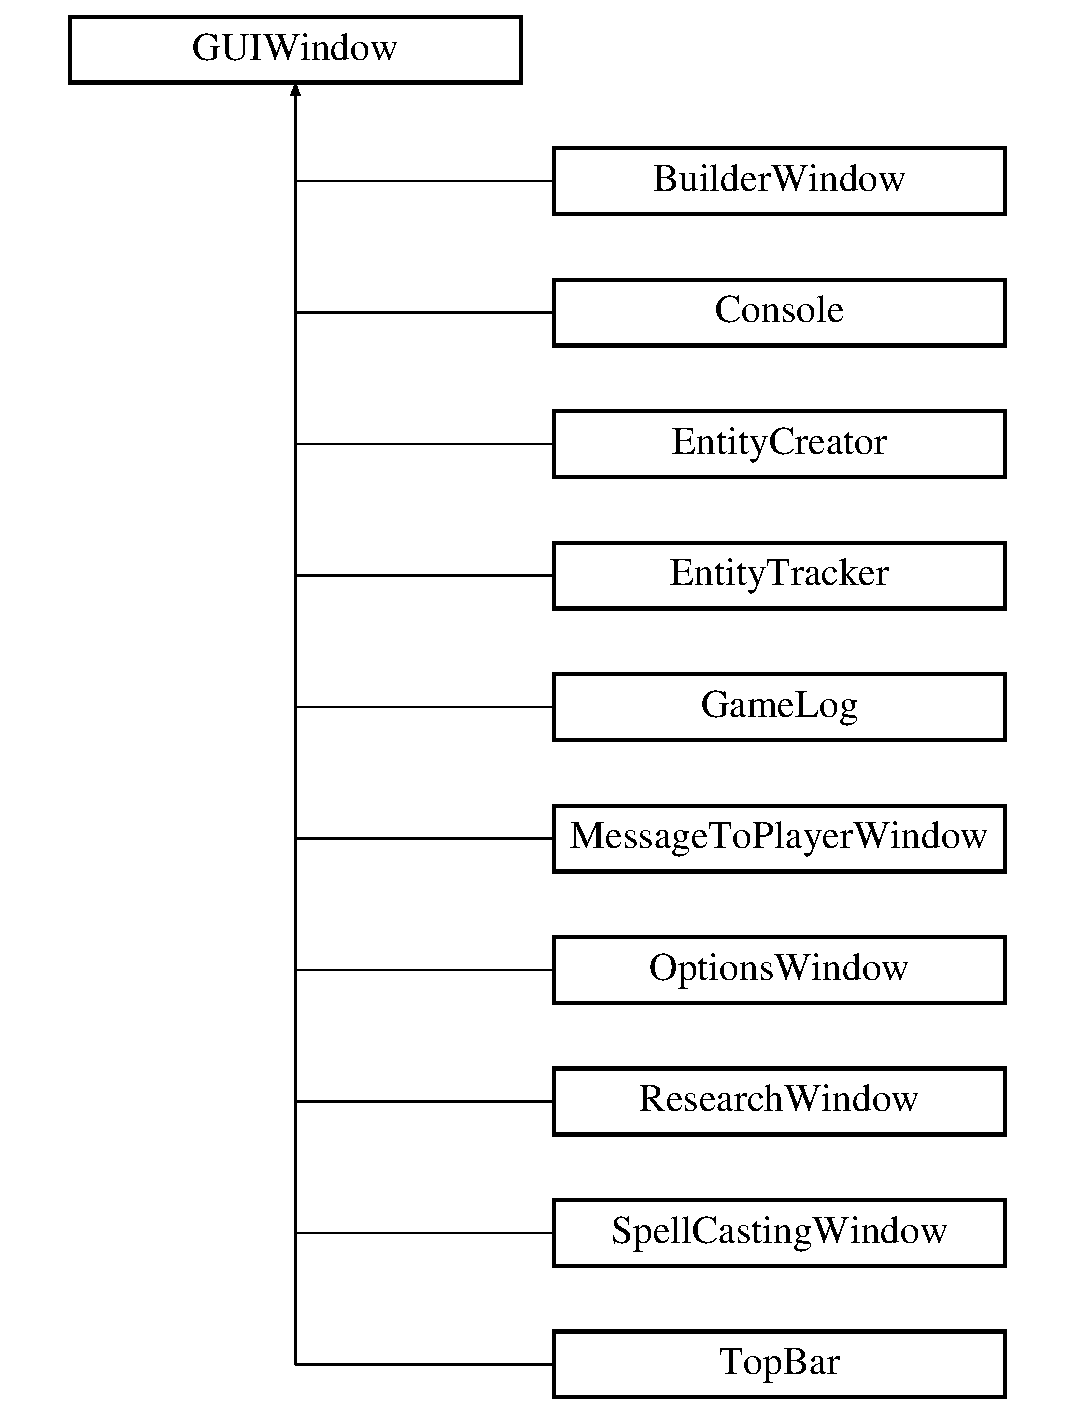
\includegraphics[height=11.000000cm]{class_g_u_i_window}
\end{center}
\end{figure}
\subsection*{Public Member Functions}
\begin{DoxyCompactItemize}
\item 
\hyperlink{class_g_u_i_window_a1d5f55e836dbe199acf6c6226d3793ec}{G\+U\+I\+Window} ()
\begin{DoxyCompactList}\small\item\em Constructor. \end{DoxyCompactList}\item 
virtual \hyperlink{class_g_u_i_window_a128001b8c20994f3b6b19271d11e5ec7}{$\sim$\+G\+U\+I\+Window} ()=default
\begin{DoxyCompactList}\small\item\em Destructor. \end{DoxyCompactList}\item 
void \hyperlink{class_g_u_i_window_ab5853dcaebef10aae4d625f5a0e7510d}{init} (C\+E\+G\+U\+I\+::\+Window $\ast$)
\begin{DoxyCompactList}\small\item\em Initializes the window\+\_\+ variable and calls the protected init\+\_\+ function. \end{DoxyCompactList}\item 
virtual void \hyperlink{class_g_u_i_window_afaa290bb3bb0020e676bb546d942e528}{set\+\_\+visible} (bool)
\begin{DoxyCompactList}\small\item\em Sets the visibolity status of this window. \end{DoxyCompactList}\item 
bool \hyperlink{class_g_u_i_window_af1d24e2d77fe3755db729059110d7a6c}{is\+\_\+visible} () const 
\begin{DoxyCompactList}\small\item\em Returns true if the window is visible, false otherwise. \end{DoxyCompactList}\end{DoxyCompactItemize}
\subsection*{Protected Member Functions}
\begin{DoxyCompactItemize}
\item 
virtual void \hyperlink{class_g_u_i_window_a2a7c011363f401a57a26cc7c7652bdfd}{init\+\_\+} ()=0
\begin{DoxyCompactList}\small\item\em Specific init function for each inheriting class. \end{DoxyCompactList}\end{DoxyCompactItemize}
\subsection*{Protected Attributes}
\begin{DoxyCompactItemize}
\item 
C\+E\+G\+U\+I\+::\+Window $\ast$ \hyperlink{class_g_u_i_window_ad977cc2d82b049b76ed62920123c1691}{window\+\_\+}
\begin{DoxyCompactList}\small\item\em Root window. \end{DoxyCompactList}\end{DoxyCompactItemize}


\subsection{Detailed Description}
Abstract class that custom \hyperlink{class_g_u_i}{G\+UI} windows inherit from, prevents unnecessary rewriting of common functions (like visibility setting and window\+\_\+ assignment on init). 

Definition at line 12 of file G\+U\+I\+Window.\+hpp.



\subsection{Constructor \& Destructor Documentation}
\index{G\+U\+I\+Window@{G\+U\+I\+Window}!G\+U\+I\+Window@{G\+U\+I\+Window}}
\index{G\+U\+I\+Window@{G\+U\+I\+Window}!G\+U\+I\+Window@{G\+U\+I\+Window}}
\subsubsection[{\texorpdfstring{G\+U\+I\+Window()}{GUIWindow()}}]{\setlength{\rightskip}{0pt plus 5cm}G\+U\+I\+Window\+::\+G\+U\+I\+Window (
\begin{DoxyParamCaption}
{}
\end{DoxyParamCaption}
)}\hypertarget{class_g_u_i_window_a1d5f55e836dbe199acf6c6226d3793ec}{}\label{class_g_u_i_window_a1d5f55e836dbe199acf6c6226d3793ec}


Constructor. 



Definition at line 4 of file G\+U\+I\+Window.\+cpp.

\index{G\+U\+I\+Window@{G\+U\+I\+Window}!````~G\+U\+I\+Window@{$\sim$\+G\+U\+I\+Window}}
\index{````~G\+U\+I\+Window@{$\sim$\+G\+U\+I\+Window}!G\+U\+I\+Window@{G\+U\+I\+Window}}
\subsubsection[{\texorpdfstring{$\sim$\+G\+U\+I\+Window()=default}{~GUIWindow()=default}}]{\setlength{\rightskip}{0pt plus 5cm}virtual G\+U\+I\+Window\+::$\sim$\+G\+U\+I\+Window (
\begin{DoxyParamCaption}
{}
\end{DoxyParamCaption}
)\hspace{0.3cm}{\ttfamily [virtual]}, {\ttfamily [default]}}\hypertarget{class_g_u_i_window_a128001b8c20994f3b6b19271d11e5ec7}{}\label{class_g_u_i_window_a128001b8c20994f3b6b19271d11e5ec7}


Destructor. 



\subsection{Member Function Documentation}
\index{G\+U\+I\+Window@{G\+U\+I\+Window}!init@{init}}
\index{init@{init}!G\+U\+I\+Window@{G\+U\+I\+Window}}
\subsubsection[{\texorpdfstring{init(\+C\+E\+G\+U\+I\+::\+Window $\ast$)}{init(CEGUI::Window *)}}]{\setlength{\rightskip}{0pt plus 5cm}void G\+U\+I\+Window\+::init (
\begin{DoxyParamCaption}
\item[{C\+E\+G\+U\+I\+::\+Window $\ast$}]{w}
\end{DoxyParamCaption}
)}\hypertarget{class_g_u_i_window_ab5853dcaebef10aae4d625f5a0e7510d}{}\label{class_g_u_i_window_ab5853dcaebef10aae4d625f5a0e7510d}


Initializes the window\+\_\+ variable and calls the protected init\+\_\+ function. 



Definition at line 8 of file G\+U\+I\+Window.\+cpp.

\index{G\+U\+I\+Window@{G\+U\+I\+Window}!init\+\_\+@{init\+\_\+}}
\index{init\+\_\+@{init\+\_\+}!G\+U\+I\+Window@{G\+U\+I\+Window}}
\subsubsection[{\texorpdfstring{init\+\_\+()=0}{init_()=0}}]{\setlength{\rightskip}{0pt plus 5cm}virtual void G\+U\+I\+Window\+::init\+\_\+ (
\begin{DoxyParamCaption}
{}
\end{DoxyParamCaption}
)\hspace{0.3cm}{\ttfamily [protected]}, {\ttfamily [pure virtual]}}\hypertarget{class_g_u_i_window_a2a7c011363f401a57a26cc7c7652bdfd}{}\label{class_g_u_i_window_a2a7c011363f401a57a26cc7c7652bdfd}


Specific init function for each inheriting class. 



Implemented in \hyperlink{class_spell_casting_window_a49a11d637aeef3e71036c3af9e459088}{Spell\+Casting\+Window}, \hyperlink{class_console_a55d92d149dba54c67855540d5e37c9f2}{Console}, \hyperlink{class_research_window_ac47f66b9c25ddf9076c68196296120f9}{Research\+Window}, \hyperlink{class_builder_window_aadd9fb46ddd55ce86bff0f012f56f2e8}{Builder\+Window}, \hyperlink{class_entity_tracker_a4a1051b7efd0414225bd6b19b24bf5b1}{Entity\+Tracker}, \hyperlink{class_entity_creator_a6450f0e4239b4eb3dc3c8224371c564f}{Entity\+Creator}, \hyperlink{class_message_to_player_window_a5eb87ad777baa5c23a3cdb262512d9e3}{Message\+To\+Player\+Window}, \hyperlink{class_options_window_a88bfc1401a1113e4ab4afdb8af106682}{Options\+Window}, \hyperlink{class_game_log_a0b7b3e3cfc91e0b433abdfd286c22b58}{Game\+Log}, and \hyperlink{class_top_bar_a5e3a678d8c38ee488def54f9d2ce49f0}{Top\+Bar}.

\index{G\+U\+I\+Window@{G\+U\+I\+Window}!is\+\_\+visible@{is\+\_\+visible}}
\index{is\+\_\+visible@{is\+\_\+visible}!G\+U\+I\+Window@{G\+U\+I\+Window}}
\subsubsection[{\texorpdfstring{is\+\_\+visible() const }{is_visible() const }}]{\setlength{\rightskip}{0pt plus 5cm}bool G\+U\+I\+Window\+::is\+\_\+visible (
\begin{DoxyParamCaption}
{}
\end{DoxyParamCaption}
) const}\hypertarget{class_g_u_i_window_af1d24e2d77fe3755db729059110d7a6c}{}\label{class_g_u_i_window_af1d24e2d77fe3755db729059110d7a6c}


Returns true if the window is visible, false otherwise. 



Definition at line 19 of file G\+U\+I\+Window.\+cpp.

\index{G\+U\+I\+Window@{G\+U\+I\+Window}!set\+\_\+visible@{set\+\_\+visible}}
\index{set\+\_\+visible@{set\+\_\+visible}!G\+U\+I\+Window@{G\+U\+I\+Window}}
\subsubsection[{\texorpdfstring{set\+\_\+visible(bool)}{set_visible(bool)}}]{\setlength{\rightskip}{0pt plus 5cm}void G\+U\+I\+Window\+::set\+\_\+visible (
\begin{DoxyParamCaption}
\item[{bool}]{val}
\end{DoxyParamCaption}
)\hspace{0.3cm}{\ttfamily [virtual]}}\hypertarget{class_g_u_i_window_afaa290bb3bb0020e676bb546d942e528}{}\label{class_g_u_i_window_afaa290bb3bb0020e676bb546d942e528}


Sets the visibolity status of this window. 


\begin{DoxyParams}{Parameters}
{\em The} & new visibility status. \\
\hline
\end{DoxyParams}


Reimplemented in \hyperlink{class_console_a501dafcea40b76808dec9fce5817f54a}{Console}.



Definition at line 14 of file G\+U\+I\+Window.\+cpp.



\subsection{Member Data Documentation}
\index{G\+U\+I\+Window@{G\+U\+I\+Window}!window\+\_\+@{window\+\_\+}}
\index{window\+\_\+@{window\+\_\+}!G\+U\+I\+Window@{G\+U\+I\+Window}}
\subsubsection[{\texorpdfstring{window\+\_\+}{window_}}]{\setlength{\rightskip}{0pt plus 5cm}C\+E\+G\+U\+I\+::\+Window$\ast$ G\+U\+I\+Window\+::window\+\_\+\hspace{0.3cm}{\ttfamily [protected]}}\hypertarget{class_g_u_i_window_ad977cc2d82b049b76ed62920123c1691}{}\label{class_g_u_i_window_ad977cc2d82b049b76ed62920123c1691}


Root window. 



Definition at line 47 of file G\+U\+I\+Window.\+hpp.



The documentation for this class was generated from the following files\+:\begin{DoxyCompactItemize}
\item 
gui/G\+U\+I\+Window.\+hpp\item 
gui/G\+U\+I\+Window.\+cpp\end{DoxyCompactItemize}

\hypertarget{structutil_1_1_h_a_s___g_o_l_d}{}\section{util\+:\+:H\+A\+S\+\_\+\+G\+O\+LD Struct Reference}
\label{structutil_1_1_h_a_s___g_o_l_d}\index{util\+::\+H\+A\+S\+\_\+\+G\+O\+LD@{util\+::\+H\+A\+S\+\_\+\+G\+O\+LD}}


Tests if a given entity has a gold component.  




{\ttfamily \#include $<$Util.\+hpp$>$}

\subsection*{Public Member Functions}
\begin{DoxyCompactItemize}
\item 
\hyperlink{structutil_1_1_h_a_s___g_o_l_d_a2678d4a6c013ad31ec6ea9c19584aa13}{H\+A\+S\+\_\+\+G\+O\+LD} (\hyperlink{class_entity_system}{Entity\+System} \&)
\begin{DoxyCompactList}\small\item\em Constructor. \end{DoxyCompactList}\item 
\hyperlink{structutil_1_1_h_a_s___g_o_l_d_a6ef2267d28435117f7cec3b2e157e56e}{$\sim$\+H\+A\+S\+\_\+\+G\+O\+LD} ()=default
\begin{DoxyCompactList}\small\item\em Destructor. \end{DoxyCompactList}\item 
bool \hyperlink{structutil_1_1_h_a_s___g_o_l_d_a6e0f0ec275fd0b6cdd1a4f03a170274f}{operator()} (tdt\+::uint)
\begin{DoxyCompactList}\small\item\em Tests if a given entity has a gold component. \end{DoxyCompactList}\end{DoxyCompactItemize}
\subsection*{Private Attributes}
\begin{DoxyCompactItemize}
\item 
\hyperlink{class_entity_system}{Entity\+System} \& \hyperlink{structutil_1_1_h_a_s___g_o_l_d_a2201e48e29a16c4ede9d07b2b0f7b430}{entities\+\_\+}
\begin{DoxyCompactList}\small\item\em Entity system containing all tested entities. \end{DoxyCompactList}\end{DoxyCompactItemize}


\subsection{Detailed Description}
Tests if a given entity has a gold component. 

Definition at line 132 of file Util.\+hpp.



\subsection{Constructor \& Destructor Documentation}
\index{util\+::\+H\+A\+S\+\_\+\+G\+O\+LD@{util\+::\+H\+A\+S\+\_\+\+G\+O\+LD}!H\+A\+S\+\_\+\+G\+O\+LD@{H\+A\+S\+\_\+\+G\+O\+LD}}
\index{H\+A\+S\+\_\+\+G\+O\+LD@{H\+A\+S\+\_\+\+G\+O\+LD}!util\+::\+H\+A\+S\+\_\+\+G\+O\+LD@{util\+::\+H\+A\+S\+\_\+\+G\+O\+LD}}
\subsubsection[{\texorpdfstring{H\+A\+S\+\_\+\+G\+O\+L\+D(\+Entity\+System \&)}{HAS_GOLD(EntitySystem &)}}]{\setlength{\rightskip}{0pt plus 5cm}util\+::\+H\+A\+S\+\_\+\+G\+O\+L\+D\+::\+H\+A\+S\+\_\+\+G\+O\+LD (
\begin{DoxyParamCaption}
\item[{{\bf Entity\+System} \&}]{ents}
\end{DoxyParamCaption}
)}\hypertarget{structutil_1_1_h_a_s___g_o_l_d_a2678d4a6c013ad31ec6ea9c19584aa13}{}\label{structutil_1_1_h_a_s___g_o_l_d_a2678d4a6c013ad31ec6ea9c19584aa13}


Constructor. 


\begin{DoxyParams}{Parameters}
{\em Entity} & system containing all tested entities. \\
\hline
\end{DoxyParams}


Definition at line 45 of file Util.\+cpp.

\index{util\+::\+H\+A\+S\+\_\+\+G\+O\+LD@{util\+::\+H\+A\+S\+\_\+\+G\+O\+LD}!````~H\+A\+S\+\_\+\+G\+O\+LD@{$\sim$\+H\+A\+S\+\_\+\+G\+O\+LD}}
\index{````~H\+A\+S\+\_\+\+G\+O\+LD@{$\sim$\+H\+A\+S\+\_\+\+G\+O\+LD}!util\+::\+H\+A\+S\+\_\+\+G\+O\+LD@{util\+::\+H\+A\+S\+\_\+\+G\+O\+LD}}
\subsubsection[{\texorpdfstring{$\sim$\+H\+A\+S\+\_\+\+G\+O\+L\+D()=default}{~HAS_GOLD()=default}}]{\setlength{\rightskip}{0pt plus 5cm}util\+::\+H\+A\+S\+\_\+\+G\+O\+L\+D\+::$\sim$\+H\+A\+S\+\_\+\+G\+O\+LD (
\begin{DoxyParamCaption}
{}
\end{DoxyParamCaption}
)\hspace{0.3cm}{\ttfamily [default]}}\hypertarget{structutil_1_1_h_a_s___g_o_l_d_a6ef2267d28435117f7cec3b2e157e56e}{}\label{structutil_1_1_h_a_s___g_o_l_d_a6ef2267d28435117f7cec3b2e157e56e}


Destructor. 



\subsection{Member Function Documentation}
\index{util\+::\+H\+A\+S\+\_\+\+G\+O\+LD@{util\+::\+H\+A\+S\+\_\+\+G\+O\+LD}!operator()@{operator()}}
\index{operator()@{operator()}!util\+::\+H\+A\+S\+\_\+\+G\+O\+LD@{util\+::\+H\+A\+S\+\_\+\+G\+O\+LD}}
\subsubsection[{\texorpdfstring{operator()(tdt\+::uint)}{operator()(tdt::uint)}}]{\setlength{\rightskip}{0pt plus 5cm}bool util\+::\+H\+A\+S\+\_\+\+G\+O\+L\+D\+::operator() (
\begin{DoxyParamCaption}
\item[{tdt\+::uint}]{id}
\end{DoxyParamCaption}
)}\hypertarget{structutil_1_1_h_a_s___g_o_l_d_a6e0f0ec275fd0b6cdd1a4f03a170274f}{}\label{structutil_1_1_h_a_s___g_o_l_d_a6e0f0ec275fd0b6cdd1a4f03a170274f}


Tests if a given entity has a gold component. 


\begin{DoxyParams}{Parameters}
{\em ID} & of the entity. \\
\hline
\end{DoxyParams}


Definition at line 49 of file Util.\+cpp.



\subsection{Member Data Documentation}
\index{util\+::\+H\+A\+S\+\_\+\+G\+O\+LD@{util\+::\+H\+A\+S\+\_\+\+G\+O\+LD}!entities\+\_\+@{entities\+\_\+}}
\index{entities\+\_\+@{entities\+\_\+}!util\+::\+H\+A\+S\+\_\+\+G\+O\+LD@{util\+::\+H\+A\+S\+\_\+\+G\+O\+LD}}
\subsubsection[{\texorpdfstring{entities\+\_\+}{entities_}}]{\setlength{\rightskip}{0pt plus 5cm}{\bf Entity\+System}\& util\+::\+H\+A\+S\+\_\+\+G\+O\+L\+D\+::entities\+\_\+\hspace{0.3cm}{\ttfamily [private]}}\hypertarget{structutil_1_1_h_a_s___g_o_l_d_a2201e48e29a16c4ede9d07b2b0f7b430}{}\label{structutil_1_1_h_a_s___g_o_l_d_a2201e48e29a16c4ede9d07b2b0f7b430}


Entity system containing all tested entities. 



Definition at line 155 of file Util.\+hpp.



The documentation for this struct was generated from the following files\+:\begin{DoxyCompactItemize}
\item 
tools/Util.\+hpp\item 
tools/Util.\+cpp\end{DoxyCompactItemize}

\hypertarget{structutil_1_1effect_1_1_h_e_a_l___e_f_f_e_c_t}{}\section{util\+:\+:effect\+:\+:H\+E\+A\+L\+\_\+\+E\+F\+F\+E\+CT Struct Reference}
\label{structutil_1_1effect_1_1_h_e_a_l___e_f_f_e_c_t}\index{util\+::effect\+::\+H\+E\+A\+L\+\_\+\+E\+F\+F\+E\+CT@{util\+::effect\+::\+H\+E\+A\+L\+\_\+\+E\+F\+F\+E\+CT}}


Fully heals the entity it\textquotesingle{}s called on.  




{\ttfamily \#include $<$Effects.\+hpp$>$}

\subsection*{Public Member Functions}
\begin{DoxyCompactItemize}
\item 
\hyperlink{structutil_1_1effect_1_1_h_e_a_l___e_f_f_e_c_t_ac34dbe9273e3b9d4be6cd79932c8cf1e}{H\+E\+A\+L\+\_\+\+E\+F\+F\+E\+CT} (\hyperlink{class_entity_system}{Entity\+System} \&)
\begin{DoxyCompactList}\small\item\em Constructor. \end{DoxyCompactList}\item 
\hyperlink{structutil_1_1effect_1_1_h_e_a_l___e_f_f_e_c_t_ac0ab236d3a4c96517de10051d7d140fd}{$\sim$\+H\+E\+A\+L\+\_\+\+E\+F\+F\+E\+CT} ()=default
\begin{DoxyCompactList}\small\item\em Destructor. \end{DoxyCompactList}\item 
void \hyperlink{structutil_1_1effect_1_1_h_e_a_l___e_f_f_e_c_t_a832e397aafe403970d73e480b29c5004}{operator()} (tdt\+::uint)
\begin{DoxyCompactList}\small\item\em Fully heals a given entity. \end{DoxyCompactList}\end{DoxyCompactItemize}
\subsection*{Private Attributes}
\begin{DoxyCompactItemize}
\item 
\hyperlink{class_entity_system}{Entity\+System} \& \hyperlink{structutil_1_1effect_1_1_h_e_a_l___e_f_f_e_c_t_a6e7bfe3f3e1605de6bbb52f21de56b49}{entities\+\_\+}
\begin{DoxyCompactList}\small\item\em Entity system containing the entities this effect will be called on. \end{DoxyCompactList}\end{DoxyCompactItemize}


\subsection{Detailed Description}
Fully heals the entity it\textquotesingle{}s called on. 

Definition at line 61 of file Effects.\+hpp.



\subsection{Constructor \& Destructor Documentation}
\index{util\+::effect\+::\+H\+E\+A\+L\+\_\+\+E\+F\+F\+E\+CT@{util\+::effect\+::\+H\+E\+A\+L\+\_\+\+E\+F\+F\+E\+CT}!H\+E\+A\+L\+\_\+\+E\+F\+F\+E\+CT@{H\+E\+A\+L\+\_\+\+E\+F\+F\+E\+CT}}
\index{H\+E\+A\+L\+\_\+\+E\+F\+F\+E\+CT@{H\+E\+A\+L\+\_\+\+E\+F\+F\+E\+CT}!util\+::effect\+::\+H\+E\+A\+L\+\_\+\+E\+F\+F\+E\+CT@{util\+::effect\+::\+H\+E\+A\+L\+\_\+\+E\+F\+F\+E\+CT}}
\subsubsection[{\texorpdfstring{H\+E\+A\+L\+\_\+\+E\+F\+F\+E\+C\+T(\+Entity\+System \&)}{HEAL_EFFECT(EntitySystem &)}}]{\setlength{\rightskip}{0pt plus 5cm}util\+::effect\+::\+H\+E\+A\+L\+\_\+\+E\+F\+F\+E\+C\+T\+::\+H\+E\+A\+L\+\_\+\+E\+F\+F\+E\+CT (
\begin{DoxyParamCaption}
\item[{{\bf Entity\+System} \&}]{ents}
\end{DoxyParamCaption}
)}\hypertarget{structutil_1_1effect_1_1_h_e_a_l___e_f_f_e_c_t_ac34dbe9273e3b9d4be6cd79932c8cf1e}{}\label{structutil_1_1effect_1_1_h_e_a_l___e_f_f_e_c_t_ac34dbe9273e3b9d4be6cd79932c8cf1e}


Constructor. 


\begin{DoxyParams}{Parameters}
{\em Entity} & system containing the entities this effect will be called on. \\
\hline
\end{DoxyParams}


Definition at line 16 of file Effects.\+cpp.

\index{util\+::effect\+::\+H\+E\+A\+L\+\_\+\+E\+F\+F\+E\+CT@{util\+::effect\+::\+H\+E\+A\+L\+\_\+\+E\+F\+F\+E\+CT}!````~H\+E\+A\+L\+\_\+\+E\+F\+F\+E\+CT@{$\sim$\+H\+E\+A\+L\+\_\+\+E\+F\+F\+E\+CT}}
\index{````~H\+E\+A\+L\+\_\+\+E\+F\+F\+E\+CT@{$\sim$\+H\+E\+A\+L\+\_\+\+E\+F\+F\+E\+CT}!util\+::effect\+::\+H\+E\+A\+L\+\_\+\+E\+F\+F\+E\+CT@{util\+::effect\+::\+H\+E\+A\+L\+\_\+\+E\+F\+F\+E\+CT}}
\subsubsection[{\texorpdfstring{$\sim$\+H\+E\+A\+L\+\_\+\+E\+F\+F\+E\+C\+T()=default}{~HEAL_EFFECT()=default}}]{\setlength{\rightskip}{0pt plus 5cm}util\+::effect\+::\+H\+E\+A\+L\+\_\+\+E\+F\+F\+E\+C\+T\+::$\sim$\+H\+E\+A\+L\+\_\+\+E\+F\+F\+E\+CT (
\begin{DoxyParamCaption}
{}
\end{DoxyParamCaption}
)\hspace{0.3cm}{\ttfamily [default]}}\hypertarget{structutil_1_1effect_1_1_h_e_a_l___e_f_f_e_c_t_ac0ab236d3a4c96517de10051d7d140fd}{}\label{structutil_1_1effect_1_1_h_e_a_l___e_f_f_e_c_t_ac0ab236d3a4c96517de10051d7d140fd}


Destructor. 



\subsection{Member Function Documentation}
\index{util\+::effect\+::\+H\+E\+A\+L\+\_\+\+E\+F\+F\+E\+CT@{util\+::effect\+::\+H\+E\+A\+L\+\_\+\+E\+F\+F\+E\+CT}!operator()@{operator()}}
\index{operator()@{operator()}!util\+::effect\+::\+H\+E\+A\+L\+\_\+\+E\+F\+F\+E\+CT@{util\+::effect\+::\+H\+E\+A\+L\+\_\+\+E\+F\+F\+E\+CT}}
\subsubsection[{\texorpdfstring{operator()(tdt\+::uint)}{operator()(tdt::uint)}}]{\setlength{\rightskip}{0pt plus 5cm}void util\+::effect\+::\+H\+E\+A\+L\+\_\+\+E\+F\+F\+E\+C\+T\+::operator() (
\begin{DoxyParamCaption}
\item[{tdt\+::uint}]{id}
\end{DoxyParamCaption}
)}\hypertarget{structutil_1_1effect_1_1_h_e_a_l___e_f_f_e_c_t_a832e397aafe403970d73e480b29c5004}{}\label{structutil_1_1effect_1_1_h_e_a_l___e_f_f_e_c_t_a832e397aafe403970d73e480b29c5004}


Fully heals a given entity. 


\begin{DoxyParams}{Parameters}
{\em ID} & of the entity. \\
\hline
\end{DoxyParams}


Definition at line 20 of file Effects.\+cpp.



\subsection{Member Data Documentation}
\index{util\+::effect\+::\+H\+E\+A\+L\+\_\+\+E\+F\+F\+E\+CT@{util\+::effect\+::\+H\+E\+A\+L\+\_\+\+E\+F\+F\+E\+CT}!entities\+\_\+@{entities\+\_\+}}
\index{entities\+\_\+@{entities\+\_\+}!util\+::effect\+::\+H\+E\+A\+L\+\_\+\+E\+F\+F\+E\+CT@{util\+::effect\+::\+H\+E\+A\+L\+\_\+\+E\+F\+F\+E\+CT}}
\subsubsection[{\texorpdfstring{entities\+\_\+}{entities_}}]{\setlength{\rightskip}{0pt plus 5cm}{\bf Entity\+System}\& util\+::effect\+::\+H\+E\+A\+L\+\_\+\+E\+F\+F\+E\+C\+T\+::entities\+\_\+\hspace{0.3cm}{\ttfamily [private]}}\hypertarget{structutil_1_1effect_1_1_h_e_a_l___e_f_f_e_c_t_a6e7bfe3f3e1605de6bbb52f21de56b49}{}\label{structutil_1_1effect_1_1_h_e_a_l___e_f_f_e_c_t_a6e7bfe3f3e1605de6bbb52f21de56b49}


Entity system containing the entities this effect will be called on. 



Definition at line 86 of file Effects.\+hpp.



The documentation for this struct was generated from the following files\+:\begin{DoxyCompactItemize}
\item 
tools/Effects.\+hpp\item 
tools/Effects.\+cpp\end{DoxyCompactItemize}

\hypertarget{struct_health_component}{}\section{Health\+Component Struct Reference}
\label{struct_health_component}\index{Health\+Component@{Health\+Component}}


Holds info about an entity\textquotesingle{}s health and regeneration.  




{\ttfamily \#include $<$Components.\+hpp$>$}

\subsection*{Public Member Functions}
\begin{DoxyCompactItemize}
\item 
{\bfseries Health\+Component} (tdt\+::uint max=0, tdt\+::uint reg=0, tdt\+::uint def=0, bool a=true)\hypertarget{struct_health_component_af4adee45342cec889301fa47f34842b2}{}\label{struct_health_component_af4adee45342cec889301fa47f34842b2}

\item 
{\bfseries Health\+Component} (const \hyperlink{struct_health_component}{Health\+Component} \&)=default\hypertarget{struct_health_component_aeb7afb61c37d90d1254d357bf336d6b8}{}\label{struct_health_component_aeb7afb61c37d90d1254d357bf336d6b8}

\item 
{\bfseries Health\+Component} (\hyperlink{struct_health_component}{Health\+Component} \&\&)=default\hypertarget{struct_health_component_a3e7d4b1a7929533fbfba853d1fd75094}{}\label{struct_health_component_a3e7d4b1a7929533fbfba853d1fd75094}

\item 
\hyperlink{struct_health_component}{Health\+Component} \& {\bfseries operator=} (const \hyperlink{struct_health_component}{Health\+Component} \&)=default\hypertarget{struct_health_component_ab46cee5b246fc1f332375ff9eb3d3514}{}\label{struct_health_component_ab46cee5b246fc1f332375ff9eb3d3514}

\item 
\hyperlink{struct_health_component}{Health\+Component} \& {\bfseries operator=} (\hyperlink{struct_health_component}{Health\+Component} \&\&)=default\hypertarget{struct_health_component_a22e43533facb004e79376e6f105f5bfd}{}\label{struct_health_component_a22e43533facb004e79376e6f105f5bfd}

\end{DoxyCompactItemize}
\subsection*{Public Attributes}
\begin{DoxyCompactItemize}
\item 
tdt\+::uint {\bfseries curr\+\_\+hp}\hypertarget{struct_health_component_a2962b3338d598b1464984b4cf6c0e6ec}{}\label{struct_health_component_a2962b3338d598b1464984b4cf6c0e6ec}

\item 
tdt\+::uint {\bfseries max\+\_\+hp}\hypertarget{struct_health_component_af39f32766a319782781019905a204087}{}\label{struct_health_component_af39f32766a319782781019905a204087}

\item 
tdt\+::uint {\bfseries regen}\hypertarget{struct_health_component_ac064ede1ccfe8e917c190bafbaaf7a38}{}\label{struct_health_component_ac064ede1ccfe8e917c190bafbaaf7a38}

\item 
tdt\+::uint {\bfseries defense}\hypertarget{struct_health_component_a1fe173bfc3c6d95c1d7cb4acd6ecf016}{}\label{struct_health_component_a1fe173bfc3c6d95c1d7cb4acd6ecf016}

\item 
bool {\bfseries alive}\hypertarget{struct_health_component_a469e3ef8616f1563d234074b17bdbbc9}{}\label{struct_health_component_a469e3ef8616f1563d234074b17bdbbc9}

\end{DoxyCompactItemize}
\subsection*{Static Public Attributes}
\begin{DoxyCompactItemize}
\item 
static constexpr int {\bfseries type} = 1\hypertarget{struct_health_component_a06221c1e0f3a5e987f945c15e6ac15a6}{}\label{struct_health_component_a06221c1e0f3a5e987f945c15e6ac15a6}

\end{DoxyCompactItemize}


\subsection{Detailed Description}
Holds info about an entity\textquotesingle{}s health and regeneration. 

Definition at line 55 of file Components.\+hpp.



The documentation for this struct was generated from the following file\+:\begin{DoxyCompactItemize}
\item 
Components.\+hpp\end{DoxyCompactItemize}

\hypertarget{class_health_system}{}\section{Health\+System Class Reference}
\label{class_health_system}\index{Health\+System@{Health\+System}}


\hyperlink{class_system}{System} that manages the regeneration and health of entities on each frame.  




{\ttfamily \#include $<$Health\+System.\+hpp$>$}

Inheritance diagram for Health\+System\+:\begin{figure}[H]
\begin{center}
\leavevmode
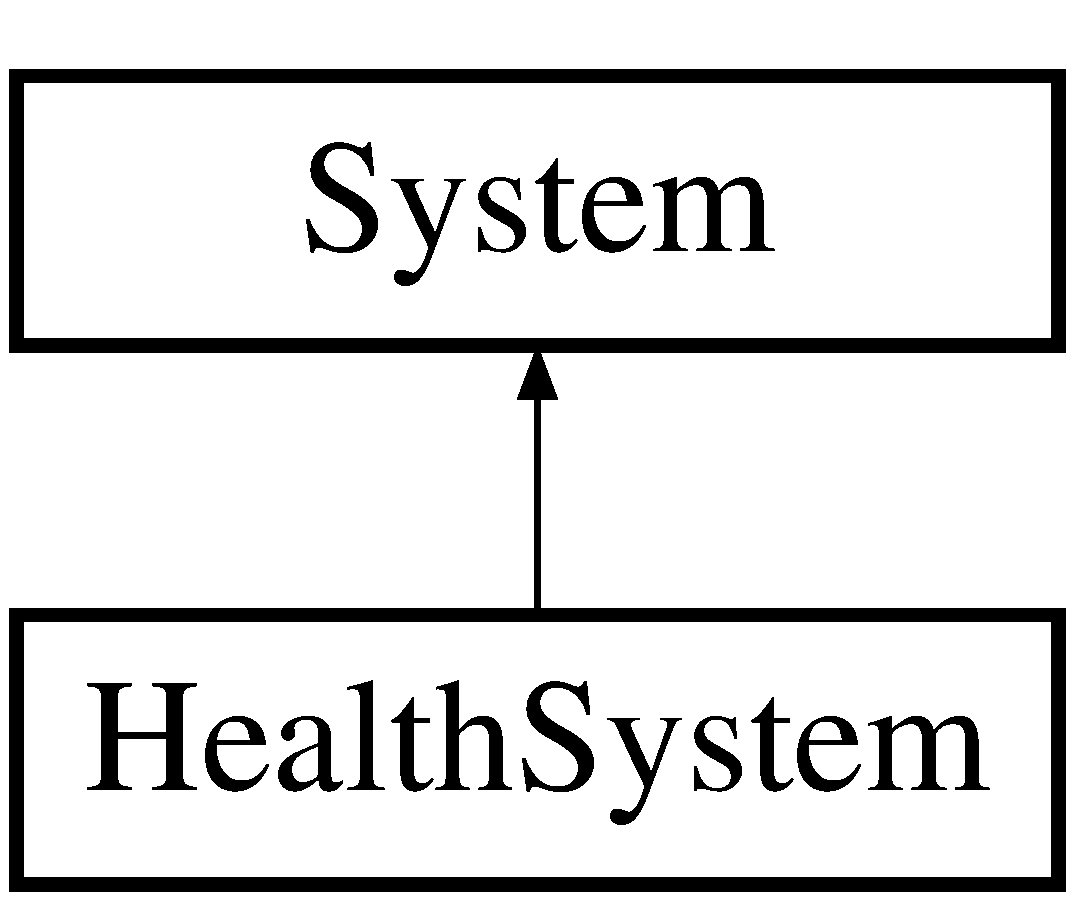
\includegraphics[height=2.000000cm]{class_health_system}
\end{center}
\end{figure}
\subsection*{Public Member Functions}
\begin{DoxyCompactItemize}
\item 
\hyperlink{class_health_system_ae843e85e6e16348860fe5cf5c5bde5b8}{Health\+System} (\hyperlink{class_entity_system}{Entity\+System} \&)
\begin{DoxyCompactList}\small\item\em Constructor. \end{DoxyCompactList}\item 
\hyperlink{class_health_system_a843b4d2e235533ab614e68826e47edf0}{$\sim$\+Health\+System} ()=default
\begin{DoxyCompactList}\small\item\em Destructor. \end{DoxyCompactList}\item 
void \hyperlink{class_health_system_a20f7adc2c2ab6e92ba8dd02e3ec95ba2}{update} (tdt\+::real) override
\begin{DoxyCompactList}\small\item\em Updates a the system by checking every valid entity\textquotesingle{}s health (or death) status and applying health regeneration if necessary. \end{DoxyCompactList}\item 
void \hyperlink{class_health_system_ade496933a64a34085c1169bcff1f2607}{update\+\_\+regen} (tdt\+::real)
\begin{DoxyCompactList}\small\item\em Adds one to the regeneration timer, simulating continuous regeration, should be called once per frame before the update method. \end{DoxyCompactList}\item 
void \hyperlink{class_health_system_ad5ae1e0a7099513a0c77bed14c92852c}{set\+\_\+regen\+\_\+period} (tdt\+::real)
\begin{DoxyCompactList}\small\item\em Sets the amount of time it takes for one regeneration tick to happen (in seconds). \end{DoxyCompactList}\item 
tdt\+::real \hyperlink{class_health_system_af2cbc492357afd14e815e14aa9dabda1}{get\+\_\+regen\+\_\+period} () const 
\begin{DoxyCompactList}\small\item\em Returns the amount of time it takes for one regeneration tick to happen (in seconds). \end{DoxyCompactList}\end{DoxyCompactItemize}
\subsection*{Private Attributes}
\begin{DoxyCompactItemize}
\item 
\hyperlink{class_entity_system}{Entity\+System} \& \hyperlink{class_health_system_a954dfb60b0452f898186781bdc5be28c}{entities\+\_\+}
\begin{DoxyCompactList}\small\item\em Reference to the game\textquotesingle{}s entity system. \end{DoxyCompactList}\item 
tdt\+::real \hyperlink{class_health_system_aa17a75833ba090bd1c0d1cd77d694bca}{regen\+\_\+timer\+\_\+}
\begin{DoxyCompactList}\small\item\em Amount of frames since the last regeneration tick. \end{DoxyCompactList}\item 
tdt\+::real \hyperlink{class_health_system_a20a6116c6307492bc38e892bafaca0f3}{regen\+\_\+period\+\_\+}
\begin{DoxyCompactList}\small\item\em Amount of frames per regeneration period. \end{DoxyCompactList}\item 
bool \hyperlink{class_health_system_a80ce11376a9356ddb1edb010806655d4}{regen\+\_\+}
\begin{DoxyCompactList}\small\item\em True if this frame\textquotesingle{}s update should renerate health. \end{DoxyCompactList}\end{DoxyCompactItemize}


\subsection{Detailed Description}
\hyperlink{class_system}{System} that manages the regeneration and health of entities on each frame. 

Definition at line 11 of file Health\+System.\+hpp.



\subsection{Constructor \& Destructor Documentation}
\index{Health\+System@{Health\+System}!Health\+System@{Health\+System}}
\index{Health\+System@{Health\+System}!Health\+System@{Health\+System}}
\subsubsection[{\texorpdfstring{Health\+System(\+Entity\+System \&)}{HealthSystem(EntitySystem &)}}]{\setlength{\rightskip}{0pt plus 5cm}Health\+System\+::\+Health\+System (
\begin{DoxyParamCaption}
\item[{{\bf Entity\+System} \&}]{ent}
\end{DoxyParamCaption}
)}\hypertarget{class_health_system_ae843e85e6e16348860fe5cf5c5bde5b8}{}\label{class_health_system_ae843e85e6e16348860fe5cf5c5bde5b8}


Constructor. 


\begin{DoxyParams}{Parameters}
{\em Reference} & to the game\textquotesingle{}s entity system. \\
\hline
\end{DoxyParams}


Definition at line 6 of file Health\+System.\+cpp.

\index{Health\+System@{Health\+System}!````~Health\+System@{$\sim$\+Health\+System}}
\index{````~Health\+System@{$\sim$\+Health\+System}!Health\+System@{Health\+System}}
\subsubsection[{\texorpdfstring{$\sim$\+Health\+System()=default}{~HealthSystem()=default}}]{\setlength{\rightskip}{0pt plus 5cm}Health\+System\+::$\sim$\+Health\+System (
\begin{DoxyParamCaption}
{}
\end{DoxyParamCaption}
)\hspace{0.3cm}{\ttfamily [default]}}\hypertarget{class_health_system_a843b4d2e235533ab614e68826e47edf0}{}\label{class_health_system_a843b4d2e235533ab614e68826e47edf0}


Destructor. 



\subsection{Member Function Documentation}
\index{Health\+System@{Health\+System}!get\+\_\+regen\+\_\+period@{get\+\_\+regen\+\_\+period}}
\index{get\+\_\+regen\+\_\+period@{get\+\_\+regen\+\_\+period}!Health\+System@{Health\+System}}
\subsubsection[{\texorpdfstring{get\+\_\+regen\+\_\+period() const }{get_regen_period() const }}]{\setlength{\rightskip}{0pt plus 5cm}tdt\+::real Health\+System\+::get\+\_\+regen\+\_\+period (
\begin{DoxyParamCaption}
{}
\end{DoxyParamCaption}
) const}\hypertarget{class_health_system_af2cbc492357afd14e815e14aa9dabda1}{}\label{class_health_system_af2cbc492357afd14e815e14aa9dabda1}


Returns the amount of time it takes for one regeneration tick to happen (in seconds). 



Definition at line 43 of file Health\+System.\+cpp.

\index{Health\+System@{Health\+System}!set\+\_\+regen\+\_\+period@{set\+\_\+regen\+\_\+period}}
\index{set\+\_\+regen\+\_\+period@{set\+\_\+regen\+\_\+period}!Health\+System@{Health\+System}}
\subsubsection[{\texorpdfstring{set\+\_\+regen\+\_\+period(tdt\+::real)}{set_regen_period(tdt::real)}}]{\setlength{\rightskip}{0pt plus 5cm}void Health\+System\+::set\+\_\+regen\+\_\+period (
\begin{DoxyParamCaption}
\item[{tdt\+::real}]{val}
\end{DoxyParamCaption}
)}\hypertarget{class_health_system_ad5ae1e0a7099513a0c77bed14c92852c}{}\label{class_health_system_ad5ae1e0a7099513a0c77bed14c92852c}


Sets the amount of time it takes for one regeneration tick to happen (in seconds). 


\begin{DoxyParams}{Parameters}
{\em The} & new regen period. \\
\hline
\end{DoxyParams}


Definition at line 38 of file Health\+System.\+cpp.

\index{Health\+System@{Health\+System}!update@{update}}
\index{update@{update}!Health\+System@{Health\+System}}
\subsubsection[{\texorpdfstring{update(tdt\+::real) override}{update(tdt::real) override}}]{\setlength{\rightskip}{0pt plus 5cm}void Health\+System\+::update (
\begin{DoxyParamCaption}
\item[{tdt\+::real}]{delta}
\end{DoxyParamCaption}
)\hspace{0.3cm}{\ttfamily [override]}, {\ttfamily [virtual]}}\hypertarget{class_health_system_a20f7adc2c2ab6e92ba8dd02e3ec95ba2}{}\label{class_health_system_a20f7adc2c2ab6e92ba8dd02e3ec95ba2}


Updates a the system by checking every valid entity\textquotesingle{}s health (or death) status and applying health regeneration if necessary. 


\begin{DoxyParams}{Parameters}
{\em Time} & since the last frame. \\
\hline
\end{DoxyParams}


Implements \hyperlink{class_system_a6d54c9bd38eb43d620a1451cb0925472}{System}.



Definition at line 11 of file Health\+System.\+cpp.

\index{Health\+System@{Health\+System}!update\+\_\+regen@{update\+\_\+regen}}
\index{update\+\_\+regen@{update\+\_\+regen}!Health\+System@{Health\+System}}
\subsubsection[{\texorpdfstring{update\+\_\+regen(tdt\+::real)}{update_regen(tdt::real)}}]{\setlength{\rightskip}{0pt plus 5cm}void Health\+System\+::update\+\_\+regen (
\begin{DoxyParamCaption}
\item[{tdt\+::real}]{delta}
\end{DoxyParamCaption}
)}\hypertarget{class_health_system_ade496933a64a34085c1169bcff1f2607}{}\label{class_health_system_ade496933a64a34085c1169bcff1f2607}


Adds one to the regeneration timer, simulating continuous regeration, should be called once per frame before the update method. 


\begin{DoxyParams}{Parameters}
{\em Time} & since the last frame. \\
\hline
\end{DoxyParams}


Definition at line 23 of file Health\+System.\+cpp.



\subsection{Member Data Documentation}
\index{Health\+System@{Health\+System}!entities\+\_\+@{entities\+\_\+}}
\index{entities\+\_\+@{entities\+\_\+}!Health\+System@{Health\+System}}
\subsubsection[{\texorpdfstring{entities\+\_\+}{entities_}}]{\setlength{\rightskip}{0pt plus 5cm}{\bf Entity\+System}\& Health\+System\+::entities\+\_\+\hspace{0.3cm}{\ttfamily [private]}}\hypertarget{class_health_system_a954dfb60b0452f898186781bdc5be28c}{}\label{class_health_system_a954dfb60b0452f898186781bdc5be28c}


Reference to the game\textquotesingle{}s entity system. 



Definition at line 56 of file Health\+System.\+hpp.

\index{Health\+System@{Health\+System}!regen\+\_\+@{regen\+\_\+}}
\index{regen\+\_\+@{regen\+\_\+}!Health\+System@{Health\+System}}
\subsubsection[{\texorpdfstring{regen\+\_\+}{regen_}}]{\setlength{\rightskip}{0pt plus 5cm}bool Health\+System\+::regen\+\_\+\hspace{0.3cm}{\ttfamily [private]}}\hypertarget{class_health_system_a80ce11376a9356ddb1edb010806655d4}{}\label{class_health_system_a80ce11376a9356ddb1edb010806655d4}


True if this frame\textquotesingle{}s update should renerate health. 



Definition at line 71 of file Health\+System.\+hpp.

\index{Health\+System@{Health\+System}!regen\+\_\+period\+\_\+@{regen\+\_\+period\+\_\+}}
\index{regen\+\_\+period\+\_\+@{regen\+\_\+period\+\_\+}!Health\+System@{Health\+System}}
\subsubsection[{\texorpdfstring{regen\+\_\+period\+\_\+}{regen_period_}}]{\setlength{\rightskip}{0pt plus 5cm}tdt\+::real Health\+System\+::regen\+\_\+period\+\_\+\hspace{0.3cm}{\ttfamily [private]}}\hypertarget{class_health_system_a20a6116c6307492bc38e892bafaca0f3}{}\label{class_health_system_a20a6116c6307492bc38e892bafaca0f3}


Amount of frames per regeneration period. 



Definition at line 66 of file Health\+System.\+hpp.

\index{Health\+System@{Health\+System}!regen\+\_\+timer\+\_\+@{regen\+\_\+timer\+\_\+}}
\index{regen\+\_\+timer\+\_\+@{regen\+\_\+timer\+\_\+}!Health\+System@{Health\+System}}
\subsubsection[{\texorpdfstring{regen\+\_\+timer\+\_\+}{regen_timer_}}]{\setlength{\rightskip}{0pt plus 5cm}tdt\+::real Health\+System\+::regen\+\_\+timer\+\_\+\hspace{0.3cm}{\ttfamily [private]}}\hypertarget{class_health_system_aa17a75833ba090bd1c0d1cd77d694bca}{}\label{class_health_system_aa17a75833ba090bd1c0d1cd77d694bca}


Amount of frames since the last regeneration tick. 



Definition at line 61 of file Health\+System.\+hpp.



The documentation for this class was generated from the following files\+:\begin{DoxyCompactItemize}
\item 
systems/Health\+System.\+hpp\item 
systems/Health\+System.\+cpp\end{DoxyCompactItemize}

\hypertarget{structutil_1_1heuristic_1_1_h_e_u_r_i_s_t_i_c}{}\section{util\+:\+:heuristic\+:\+:H\+E\+U\+R\+I\+S\+T\+IC Struct Reference}
\label{structutil_1_1heuristic_1_1_h_e_u_r_i_s_t_i_c}\index{util\+::heuristic\+::\+H\+E\+U\+R\+I\+S\+T\+IC@{util\+::heuristic\+::\+H\+E\+U\+R\+I\+S\+T\+IC}}


Abstract parent of all heuristics.  




{\ttfamily \#include $<$Pathfinding\+Algorithms.\+hpp$>$}

Inheritance diagram for util\+:\+:heuristic\+:\+:H\+E\+U\+R\+I\+S\+T\+IC\+:\begin{figure}[H]
\begin{center}
\leavevmode
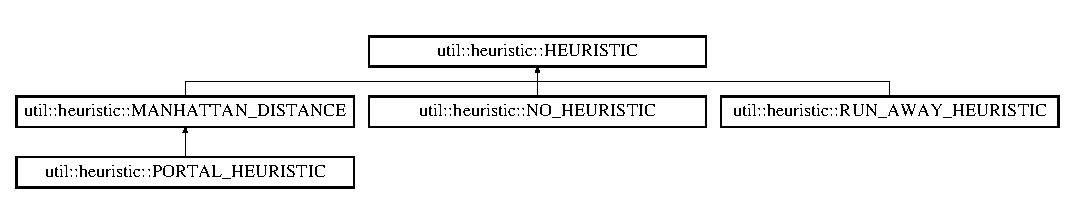
\includegraphics[height=2.295082cm]{structutil_1_1heuristic_1_1_h_e_u_r_i_s_t_i_c}
\end{center}
\end{figure}
\subsection*{Public Member Functions}
\begin{DoxyCompactItemize}
\item 
{\bfseries H\+E\+U\+R\+I\+S\+T\+IC} (\hyperlink{class_entity_system}{Entity\+System} \&ents)\hypertarget{structutil_1_1heuristic_1_1_h_e_u_r_i_s_t_i_c_a6ce8869fa7601d51172e537fd552356f}{}\label{structutil_1_1heuristic_1_1_h_e_u_r_i_s_t_i_c_a6ce8869fa7601d51172e537fd552356f}

\item 
virtual tdt\+::real {\bfseries get\+\_\+cost} (tdt\+::uint id1, tdt\+::uint id2)=0\hypertarget{structutil_1_1heuristic_1_1_h_e_u_r_i_s_t_i_c_a846e258ef0135548dcc0fdab0f6a1b79}{}\label{structutil_1_1heuristic_1_1_h_e_u_r_i_s_t_i_c_a846e258ef0135548dcc0fdab0f6a1b79}

\end{DoxyCompactItemize}
\subsection*{Protected Attributes}
\begin{DoxyCompactItemize}
\item 
\hyperlink{class_entity_system}{Entity\+System} \& {\bfseries entities\+\_\+}\hypertarget{structutil_1_1heuristic_1_1_h_e_u_r_i_s_t_i_c_aeb53f19deca6db9b8c64aca7385a2247}{}\label{structutil_1_1heuristic_1_1_h_e_u_r_i_s_t_i_c_aeb53f19deca6db9b8c64aca7385a2247}

\end{DoxyCompactItemize}


\subsection{Detailed Description}
Abstract parent of all heuristics. 

Inheritance hierarchy used instead of static functions (like in the case of P\+A\+T\+H\+\_\+\+T\+Y\+P\+Es) to allow for a heuristic to have a state. 

Definition at line 188 of file Pathfinding\+Algorithms.\+hpp.



The documentation for this struct was generated from the following file\+:\begin{DoxyCompactItemize}
\item 
tools/Pathfinding\+Algorithms.\+hpp\end{DoxyCompactItemize}

\hypertarget{struct_homing_component}{}\section{Homing\+Component Struct Reference}
\label{struct_homing_component}\index{Homing\+Component@{Homing\+Component}}


Used for projectiles that are supposed to follow a target and deal damage when they hit it.  




{\ttfamily \#include $<$Components.\+hpp$>$}

\subsection*{Public Member Functions}
\begin{DoxyCompactItemize}
\item 
{\bfseries Homing\+Component} (tdt\+::uint s=Component\+::\+N\+O\+\_\+\+E\+N\+T\+I\+TY, tdt\+::uint t=Component\+::\+N\+O\+\_\+\+E\+N\+T\+I\+TY, tdt\+::uint d=0)\hypertarget{struct_homing_component_ac91b84e8e7333c7244d9a0b983df358f}{}\label{struct_homing_component_ac91b84e8e7333c7244d9a0b983df358f}

\item 
{\bfseries Homing\+Component} (const \hyperlink{struct_homing_component}{Homing\+Component} \&)=default\hypertarget{struct_homing_component_a02790de1d791ee8780f88c4df7e89261}{}\label{struct_homing_component_a02790de1d791ee8780f88c4df7e89261}

\item 
{\bfseries Homing\+Component} (\hyperlink{struct_homing_component}{Homing\+Component} \&\&)=default\hypertarget{struct_homing_component_a9528599a073109a06454ee888232e064}{}\label{struct_homing_component_a9528599a073109a06454ee888232e064}

\item 
\hyperlink{struct_homing_component}{Homing\+Component} \& {\bfseries operator=} (const \hyperlink{struct_homing_component}{Homing\+Component} \&)=default\hypertarget{struct_homing_component_aec9487594754a223fd55717d0a2c677c}{}\label{struct_homing_component_aec9487594754a223fd55717d0a2c677c}

\item 
\hyperlink{struct_homing_component}{Homing\+Component} \& {\bfseries operator=} (\hyperlink{struct_homing_component}{Homing\+Component} \&\&)=default\hypertarget{struct_homing_component_ad7fefeec17705d1f9ad082f401e2ecb1}{}\label{struct_homing_component_ad7fefeec17705d1f9ad082f401e2ecb1}

\end{DoxyCompactItemize}
\subsection*{Public Attributes}
\begin{DoxyCompactItemize}
\item 
tdt\+::uint {\bfseries source}\hypertarget{struct_homing_component_a1cba9a813cd94e823ddc42bae1e4996b}{}\label{struct_homing_component_a1cba9a813cd94e823ddc42bae1e4996b}

\item 
tdt\+::uint {\bfseries target}\hypertarget{struct_homing_component_a71840e328968a719ea0bc1404a01b26e}{}\label{struct_homing_component_a71840e328968a719ea0bc1404a01b26e}

\item 
tdt\+::uint {\bfseries dmg}\hypertarget{struct_homing_component_a085f9ca647fbae4cbf19e12f061befba}{}\label{struct_homing_component_a085f9ca647fbae4cbf19e12f061befba}

\end{DoxyCompactItemize}
\subsection*{Static Public Attributes}
\begin{DoxyCompactItemize}
\item 
static constexpr int {\bfseries type} = 18\hypertarget{struct_homing_component_a6797c2200b17f50e39b69e9ff0d005c4}{}\label{struct_homing_component_a6797c2200b17f50e39b69e9ff0d005c4}

\end{DoxyCompactItemize}


\subsection{Detailed Description}
Used for projectiles that are supposed to follow a target and deal damage when they hit it. 

Definition at line 462 of file Components.\+hpp.



The documentation for this struct was generated from the following file\+:\begin{DoxyCompactItemize}
\item 
Components.\+hpp\end{DoxyCompactItemize}

\hypertarget{struct_input_component}{}\section{Input\+Component Struct Reference}
\label{struct_input_component}\index{Input\+Component@{Input\+Component}}


Holds info related to direct player input applied to an entity.  




{\ttfamily \#include $<$Components.\+hpp$>$}

\subsection*{Public Member Functions}
\begin{DoxyCompactItemize}
\item 
{\bfseries Input\+Component} (std\+::string \&\&handler=\char`\"{}E\+R\+R\+O\+R.\+input\+\_\+handler\char`\"{})\hypertarget{struct_input_component_ab2803ef8ff9e09f87c8426beec0c0223}{}\label{struct_input_component_ab2803ef8ff9e09f87c8426beec0c0223}

\item 
{\bfseries Input\+Component} (const \hyperlink{struct_input_component}{Input\+Component} \&)=default\hypertarget{struct_input_component_ab35d58b204fea0461f1a2df787e250f2}{}\label{struct_input_component_ab35d58b204fea0461f1a2df787e250f2}

\item 
{\bfseries Input\+Component} (\hyperlink{struct_input_component}{Input\+Component} \&\&)=default\hypertarget{struct_input_component_a27c7f78af492719184e7ad3f44df99f5}{}\label{struct_input_component_a27c7f78af492719184e7ad3f44df99f5}

\item 
\hyperlink{struct_input_component}{Input\+Component} \& {\bfseries operator=} (const \hyperlink{struct_input_component}{Input\+Component} \&)=default\hypertarget{struct_input_component_a92d7d6443d4245633235225144bcffd1}{}\label{struct_input_component_a92d7d6443d4245633235225144bcffd1}

\item 
\hyperlink{struct_input_component}{Input\+Component} \& {\bfseries operator=} (\hyperlink{struct_input_component}{Input\+Component} \&\&)=default\hypertarget{struct_input_component_a29efb3bb4e166bf7453dd8519651083c}{}\label{struct_input_component_a29efb3bb4e166bf7453dd8519651083c}

\end{DoxyCompactItemize}
\subsection*{Public Attributes}
\begin{DoxyCompactItemize}
\item 
std\+::string {\bfseries input\+\_\+handler}\hypertarget{struct_input_component_a4bba759f930669eca328242520f112e7}{}\label{struct_input_component_a4bba759f930669eca328242520f112e7}

\end{DoxyCompactItemize}
\subsection*{Static Public Attributes}
\begin{DoxyCompactItemize}
\item 
static constexpr int {\bfseries type} = 7\hypertarget{struct_input_component_a571a3e30e426f90c372919e7a585b4d9}{}\label{struct_input_component_a571a3e30e426f90c372919e7a585b4d9}

\end{DoxyCompactItemize}


\subsection{Detailed Description}
Holds info related to direct player input applied to an entity. 

Definition at line 207 of file Components.\+hpp.



The documentation for this struct was generated from the following file\+:\begin{DoxyCompactItemize}
\item 
Components.\+hpp\end{DoxyCompactItemize}

\hypertarget{class_input_system}{}\section{Input\+System Class Reference}
\label{class_input_system}\index{Input\+System@{Input\+System}}


\hyperlink{class_system}{System} handling entities controlled by the player\textquotesingle{}s keyboard input and changing the game\textquotesingle{}s view mode (between 1st and 3rd person).  




{\ttfamily \#include $<$Input\+System.\+hpp$>$}

Inheritance diagram for Input\+System\+:\begin{figure}[H]
\begin{center}
\leavevmode
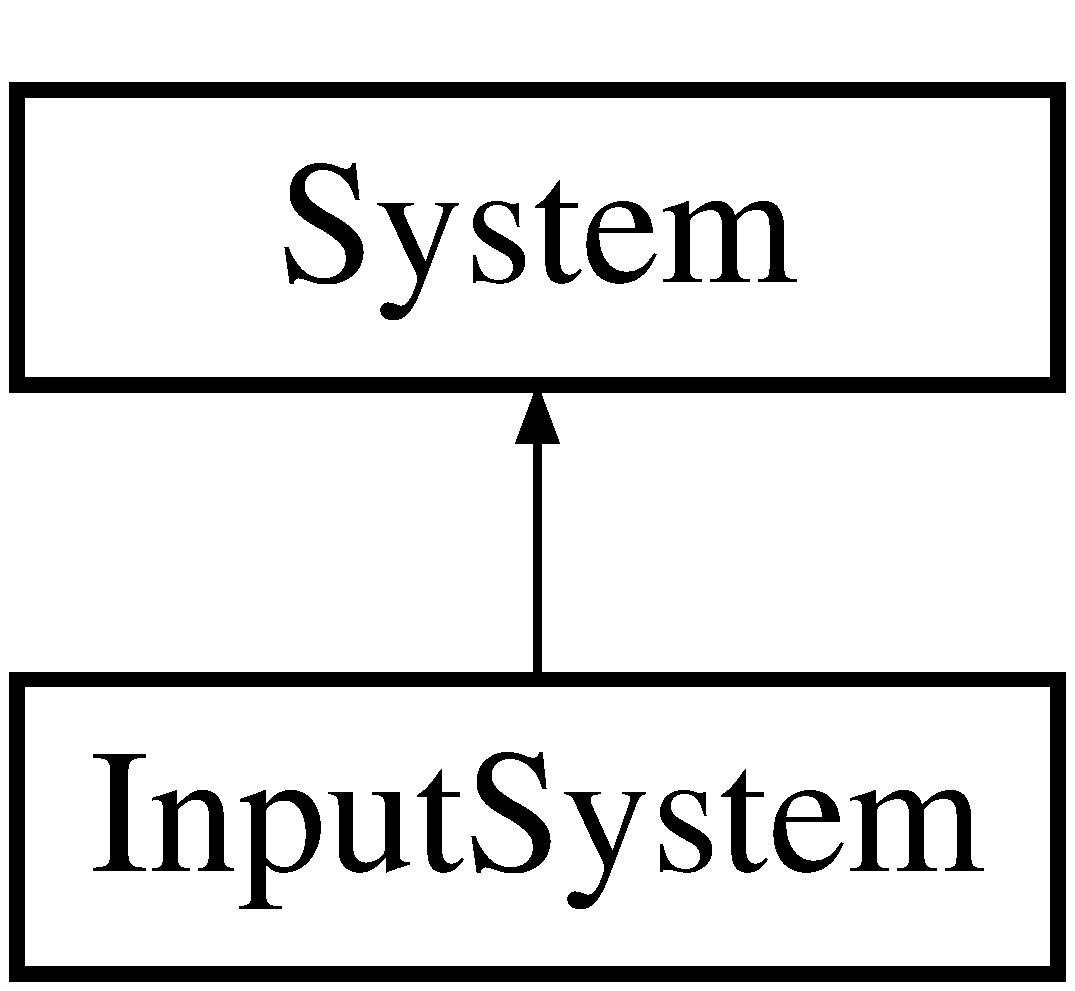
\includegraphics[height=2.000000cm]{class_input_system}
\end{center}
\end{figure}
\subsection*{Public Member Functions}
\begin{DoxyCompactItemize}
\item 
\hyperlink{class_input_system_aada2a62cbb74e5fdf669f6fb6ac4d933}{Input\+System} (\hyperlink{class_entity_system}{Entity\+System} \&, O\+I\+S\+::\+Keyboard \&, Ogre\+::\+Camera \&)
\begin{DoxyCompactList}\small\item\em Constructor. \end{DoxyCompactList}\item 
\hyperlink{class_input_system_a0d4dcf75be69044e88b17653925d35b7}{$\sim$\+Input\+System} ()=default
\begin{DoxyCompactList}\small\item\em Destructor. \end{DoxyCompactList}\item 
void \hyperlink{class_input_system_a6ee8dd556fa9352321197412b186c0c1}{update} (tdt\+::real) override
\begin{DoxyCompactList}\small\item\em Handles the input for the entity that is currently in the first person mode. \end{DoxyCompactList}\item 
bool \hyperlink{class_input_system_a6b551b82243b363066b6c309f95d8b4f}{is\+\_\+first\+\_\+person} () const 
\begin{DoxyCompactList}\small\item\em Returns true if the game is in the first person mode, returns false otherwise. \end{DoxyCompactList}\item 
void \hyperlink{class_input_system_a1784a34e02a24ef38712e5f3ef501581}{set\+\_\+first\+\_\+person} (bool, tdt\+::uint=0)
\begin{DoxyCompactList}\small\item\em Changes the first person mode status for an entity and also loads an \hyperlink{struct_input_component}{Input\+Component} for it if it does not have it but has an \hyperlink{struct_a_i_component}{A\+I\+Component} holding information about it\textquotesingle{}s input\+\_\+handler method. \end{DoxyCompactList}\item 
void \hyperlink{class_input_system_acec0ff323d487f721998975e4dc24959}{rebind} (int, int)
\begin{DoxyCompactList}\small\item\em Rebinds a given key with an O\+IS key number. \end{DoxyCompactList}\end{DoxyCompactItemize}
\subsection*{Private Attributes}
\begin{DoxyCompactItemize}
\item 
\hyperlink{class_entity_system}{Entity\+System} \& \hyperlink{class_input_system_ad7cd4d1cc1598f0d72c8531ba190ed94}{entities\+\_\+}
\begin{DoxyCompactList}\small\item\em Reference to the game\textquotesingle{}s entity system. \end{DoxyCompactList}\item 
bool \hyperlink{class_input_system_a3c7bdb083dc27e80b9d20f6f8fcedb79}{first\+\_\+person\+\_\+}
\begin{DoxyCompactList}\small\item\em Determines if the first person view is turned on. \end{DoxyCompactList}\item 
tdt\+::uint \hyperlink{class_input_system_ab6760a6b3b09cc28e564eac23ea4fd53}{first\+\_\+person\+\_\+id\+\_\+}
\begin{DoxyCompactList}\small\item\em If the first person view is turned on, this holds ID of the entity being controlled. \end{DoxyCompactList}\item 
O\+I\+S\+::\+Keyboard \& \hyperlink{class_input_system_a7b1e5fc521e98e9a4b0684fb1a9711c9}{keyboard\+\_\+}
\begin{DoxyCompactList}\small\item\em Reference to the keyboard being used. \end{DoxyCompactList}\item 
int \hyperlink{class_input_system_a28f6fccea67986967559e39cf0215c8b}{K\+E\+Y\+\_\+\+UP}
\begin{DoxyCompactList}\small\item\em Current keybindings, allow rebinding. \end{DoxyCompactList}\item 
int {\bfseries K\+E\+Y\+\_\+\+D\+O\+WN}\hypertarget{class_input_system_a450bfb7fffc6ccb8cb846b5d4380f906}{}\label{class_input_system_a450bfb7fffc6ccb8cb846b5d4380f906}

\item 
int {\bfseries K\+E\+Y\+\_\+\+L\+E\+FT}\hypertarget{class_input_system_aa78b74b66edcafd58f65205eff0f320f}{}\label{class_input_system_aa78b74b66edcafd58f65205eff0f320f}

\item 
int {\bfseries K\+E\+Y\+\_\+\+R\+I\+G\+HT}\hypertarget{class_input_system_a556ac5ca7ba4ac40ff868b3c1effbdb3}{}\label{class_input_system_a556ac5ca7ba4ac40ff868b3c1effbdb3}

\item 
Ogre\+::\+Camera \& \hyperlink{class_input_system_a7725c6f5b40f31c3bd89c55a44641cb7}{cam\+\_\+}
\begin{DoxyCompactList}\small\item\em Reference to the game\textquotesingle{}s main camera. \end{DoxyCompactList}\item 
Ogre\+::\+Vector3 \hyperlink{class_input_system_a06dc8cddfde4ecde07008cdb5bd4458e}{cam\+\_\+position\+\_\+}
\begin{DoxyCompactList}\small\item\em Backup of the camera info for easy restoring once the game leaves the first person view. \end{DoxyCompactList}\item 
Ogre\+::\+Quaternion {\bfseries cam\+\_\+orientation\+\_\+}\hypertarget{class_input_system_a76936e44fc531e9b448fdfae587bb7d0}{}\label{class_input_system_a76936e44fc531e9b448fdfae587bb7d0}

\item 
std\+::unique\+\_\+ptr$<$ \hyperlink{struct_a_i_component}{A\+I\+Component} $>$ \hyperlink{class_input_system_a4db625dcec72e55ecc0c4b0b52f5263a}{ai\+\_\+backup\+\_\+}
\begin{DoxyCompactList}\small\item\em Backup of the AI component when entering first person view. \end{DoxyCompactList}\item 
std\+::unique\+\_\+ptr$<$ \hyperlink{struct_task_handler_component}{Task\+Handler\+Component} $>$ \hyperlink{class_input_system_af5cf64f0c19712f6f792cfd75d247ad1}{task\+\_\+backup\+\_\+}
\begin{DoxyCompactList}\small\item\em Backup of the task component when entering first person view. \end{DoxyCompactList}\item 
bool \hyperlink{class_input_system_a549e0c521082a6ff97c2b9349d000cb0}{delete\+\_\+input\+\_\+}
\begin{DoxyCompactList}\small\item\em Determines if the \hyperlink{struct_input_component}{Input\+Component} of the entity being controlled in the first person view should be deleted once the game changes back to third person view. \end{DoxyCompactList}\end{DoxyCompactItemize}


\subsection{Detailed Description}
\hyperlink{class_system}{System} handling entities controlled by the player\textquotesingle{}s keyboard input and changing the game\textquotesingle{}s view mode (between 1st and 3rd person). 

Definition at line 16 of file Input\+System.\+hpp.



\subsection{Constructor \& Destructor Documentation}
\index{Input\+System@{Input\+System}!Input\+System@{Input\+System}}
\index{Input\+System@{Input\+System}!Input\+System@{Input\+System}}
\subsubsection[{\texorpdfstring{Input\+System(\+Entity\+System \&, O\+I\+S\+::\+Keyboard \&, Ogre\+::\+Camera \&)}{InputSystem(EntitySystem &, OIS::Keyboard &, Ogre::Camera &)}}]{\setlength{\rightskip}{0pt plus 5cm}Input\+System\+::\+Input\+System (
\begin{DoxyParamCaption}
\item[{{\bf Entity\+System} \&}]{ents, }
\item[{O\+I\+S\+::\+Keyboard \&}]{key, }
\item[{Ogre\+::\+Camera \&}]{cam}
\end{DoxyParamCaption}
)}\hypertarget{class_input_system_aada2a62cbb74e5fdf669f6fb6ac4d933}{}\label{class_input_system_aada2a62cbb74e5fdf669f6fb6ac4d933}


Constructor. 


\begin{DoxyParams}{Parameters}
{\em Reference} & to the game\textquotesingle{}s \hyperlink{class_entity_system}{Entity\+System} instance. \\
\hline
{\em Reference} & to the keyboard being used. \\
\hline
{\em Reference} & to the camera for it\textquotesingle{}s manipulation during the 1st person mode. \\
\hline
\end{DoxyParams}


Definition at line 5 of file Input\+System.\+cpp.

\index{Input\+System@{Input\+System}!````~Input\+System@{$\sim$\+Input\+System}}
\index{````~Input\+System@{$\sim$\+Input\+System}!Input\+System@{Input\+System}}
\subsubsection[{\texorpdfstring{$\sim$\+Input\+System()=default}{~InputSystem()=default}}]{\setlength{\rightskip}{0pt plus 5cm}Input\+System\+::$\sim$\+Input\+System (
\begin{DoxyParamCaption}
{}
\end{DoxyParamCaption}
)\hspace{0.3cm}{\ttfamily [default]}}\hypertarget{class_input_system_a0d4dcf75be69044e88b17653925d35b7}{}\label{class_input_system_a0d4dcf75be69044e88b17653925d35b7}


Destructor. 



\subsection{Member Function Documentation}
\index{Input\+System@{Input\+System}!is\+\_\+first\+\_\+person@{is\+\_\+first\+\_\+person}}
\index{is\+\_\+first\+\_\+person@{is\+\_\+first\+\_\+person}!Input\+System@{Input\+System}}
\subsubsection[{\texorpdfstring{is\+\_\+first\+\_\+person() const }{is_first_person() const }}]{\setlength{\rightskip}{0pt plus 5cm}bool Input\+System\+::is\+\_\+first\+\_\+person (
\begin{DoxyParamCaption}
{}
\end{DoxyParamCaption}
) const}\hypertarget{class_input_system_a6b551b82243b363066b6c309f95d8b4f}{}\label{class_input_system_a6b551b82243b363066b6c309f95d8b4f}


Returns true if the game is in the first person mode, returns false otherwise. 



Definition at line 56 of file Input\+System.\+cpp.

\index{Input\+System@{Input\+System}!rebind@{rebind}}
\index{rebind@{rebind}!Input\+System@{Input\+System}}
\subsubsection[{\texorpdfstring{rebind(int, int)}{rebind(int, int)}}]{\setlength{\rightskip}{0pt plus 5cm}void Input\+System\+::rebind (
\begin{DoxyParamCaption}
\item[{int}]{key, }
\item[{int}]{new\+\_\+key}
\end{DoxyParamCaption}
)}\hypertarget{class_input_system_acec0ff323d487f721998975e4dc24959}{}\label{class_input_system_acec0ff323d487f721998975e4dc24959}


Rebinds a given key with an O\+IS key number. 

Use O\+I\+S\+::\+K\+C\+\_\+W, O\+I\+S\+::\+K\+C\+\_\+S, O\+I\+S\+::\+K\+C\+\_\+A and O\+I\+S\+::\+K\+C\+\_\+D to determine which key should be rebinded. 
\begin{DoxyParams}{Parameters}
{\em Key} & to be rebinded. \\
\hline
{\em The} & new key. \\
\hline
\end{DoxyParams}


Definition at line 160 of file Input\+System.\+cpp.

\index{Input\+System@{Input\+System}!set\+\_\+first\+\_\+person@{set\+\_\+first\+\_\+person}}
\index{set\+\_\+first\+\_\+person@{set\+\_\+first\+\_\+person}!Input\+System@{Input\+System}}
\subsubsection[{\texorpdfstring{set\+\_\+first\+\_\+person(bool, tdt\+::uint=0)}{set_first_person(bool, tdt::uint=0)}}]{\setlength{\rightskip}{0pt plus 5cm}void Input\+System\+::set\+\_\+first\+\_\+person (
\begin{DoxyParamCaption}
\item[{bool}]{on\+\_\+off, }
\item[{tdt\+::uint}]{id = {\ttfamily 0}}
\end{DoxyParamCaption}
)}\hypertarget{class_input_system_a1784a34e02a24ef38712e5f3ef501581}{}\label{class_input_system_a1784a34e02a24ef38712e5f3ef501581}


Changes the first person mode status for an entity and also loads an \hyperlink{struct_input_component}{Input\+Component} for it if it does not have it but has an \hyperlink{struct_a_i_component}{A\+I\+Component} holding information about it\textquotesingle{}s input\+\_\+handler method. 

(Backups the \hyperlink{struct_a_i_component}{A\+I\+Component} in such cases and restores it when the entity leaves first person mode.) 

Definition at line 61 of file Input\+System.\+cpp.

\index{Input\+System@{Input\+System}!update@{update}}
\index{update@{update}!Input\+System@{Input\+System}}
\subsubsection[{\texorpdfstring{update(tdt\+::real) override}{update(tdt::real) override}}]{\setlength{\rightskip}{0pt plus 5cm}void Input\+System\+::update (
\begin{DoxyParamCaption}
\item[{tdt\+::real}]{delta}
\end{DoxyParamCaption}
)\hspace{0.3cm}{\ttfamily [override]}, {\ttfamily [virtual]}}\hypertarget{class_input_system_a6ee8dd556fa9352321197412b186c0c1}{}\label{class_input_system_a6ee8dd556fa9352321197412b186c0c1}


Handles the input for the entity that is currently in the first person mode. 


\begin{DoxyParams}{Parameters}
{\em Time} & since the last frame. \\
\hline
\end{DoxyParams}


Implements \hyperlink{class_system_a6d54c9bd38eb43d620a1451cb0925472}{System}.



Definition at line 12 of file Input\+System.\+cpp.



\subsection{Member Data Documentation}
\index{Input\+System@{Input\+System}!ai\+\_\+backup\+\_\+@{ai\+\_\+backup\+\_\+}}
\index{ai\+\_\+backup\+\_\+@{ai\+\_\+backup\+\_\+}!Input\+System@{Input\+System}}
\subsubsection[{\texorpdfstring{ai\+\_\+backup\+\_\+}{ai_backup_}}]{\setlength{\rightskip}{0pt plus 5cm}std\+::unique\+\_\+ptr$<${\bf A\+I\+Component}$>$ Input\+System\+::ai\+\_\+backup\+\_\+\hspace{0.3cm}{\ttfamily [private]}}\hypertarget{class_input_system_a4db625dcec72e55ecc0c4b0b52f5263a}{}\label{class_input_system_a4db625dcec72e55ecc0c4b0b52f5263a}


Backup of the AI component when entering first person view. 



Definition at line 101 of file Input\+System.\+hpp.

\index{Input\+System@{Input\+System}!cam\+\_\+@{cam\+\_\+}}
\index{cam\+\_\+@{cam\+\_\+}!Input\+System@{Input\+System}}
\subsubsection[{\texorpdfstring{cam\+\_\+}{cam_}}]{\setlength{\rightskip}{0pt plus 5cm}Ogre\+::\+Camera\& Input\+System\+::cam\+\_\+\hspace{0.3cm}{\ttfamily [private]}}\hypertarget{class_input_system_a7725c6f5b40f31c3bd89c55a44641cb7}{}\label{class_input_system_a7725c6f5b40f31c3bd89c55a44641cb7}


Reference to the game\textquotesingle{}s main camera. 



Definition at line 89 of file Input\+System.\+hpp.

\index{Input\+System@{Input\+System}!cam\+\_\+position\+\_\+@{cam\+\_\+position\+\_\+}}
\index{cam\+\_\+position\+\_\+@{cam\+\_\+position\+\_\+}!Input\+System@{Input\+System}}
\subsubsection[{\texorpdfstring{cam\+\_\+position\+\_\+}{cam_position_}}]{\setlength{\rightskip}{0pt plus 5cm}Ogre\+::\+Vector3 Input\+System\+::cam\+\_\+position\+\_\+\hspace{0.3cm}{\ttfamily [private]}}\hypertarget{class_input_system_a06dc8cddfde4ecde07008cdb5bd4458e}{}\label{class_input_system_a06dc8cddfde4ecde07008cdb5bd4458e}


Backup of the camera info for easy restoring once the game leaves the first person view. 



Definition at line 95 of file Input\+System.\+hpp.

\index{Input\+System@{Input\+System}!delete\+\_\+input\+\_\+@{delete\+\_\+input\+\_\+}}
\index{delete\+\_\+input\+\_\+@{delete\+\_\+input\+\_\+}!Input\+System@{Input\+System}}
\subsubsection[{\texorpdfstring{delete\+\_\+input\+\_\+}{delete_input_}}]{\setlength{\rightskip}{0pt plus 5cm}bool Input\+System\+::delete\+\_\+input\+\_\+\hspace{0.3cm}{\ttfamily [private]}}\hypertarget{class_input_system_a549e0c521082a6ff97c2b9349d000cb0}{}\label{class_input_system_a549e0c521082a6ff97c2b9349d000cb0}


Determines if the \hyperlink{struct_input_component}{Input\+Component} of the entity being controlled in the first person view should be deleted once the game changes back to third person view. 



Definition at line 112 of file Input\+System.\+hpp.

\index{Input\+System@{Input\+System}!entities\+\_\+@{entities\+\_\+}}
\index{entities\+\_\+@{entities\+\_\+}!Input\+System@{Input\+System}}
\subsubsection[{\texorpdfstring{entities\+\_\+}{entities_}}]{\setlength{\rightskip}{0pt plus 5cm}{\bf Entity\+System}\& Input\+System\+::entities\+\_\+\hspace{0.3cm}{\ttfamily [private]}}\hypertarget{class_input_system_ad7cd4d1cc1598f0d72c8531ba190ed94}{}\label{class_input_system_ad7cd4d1cc1598f0d72c8531ba190ed94}


Reference to the game\textquotesingle{}s entity system. 



Definition at line 64 of file Input\+System.\+hpp.

\index{Input\+System@{Input\+System}!first\+\_\+person\+\_\+@{first\+\_\+person\+\_\+}}
\index{first\+\_\+person\+\_\+@{first\+\_\+person\+\_\+}!Input\+System@{Input\+System}}
\subsubsection[{\texorpdfstring{first\+\_\+person\+\_\+}{first_person_}}]{\setlength{\rightskip}{0pt plus 5cm}bool Input\+System\+::first\+\_\+person\+\_\+\hspace{0.3cm}{\ttfamily [private]}}\hypertarget{class_input_system_a3c7bdb083dc27e80b9d20f6f8fcedb79}{}\label{class_input_system_a3c7bdb083dc27e80b9d20f6f8fcedb79}


Determines if the first person view is turned on. 



Definition at line 69 of file Input\+System.\+hpp.

\index{Input\+System@{Input\+System}!first\+\_\+person\+\_\+id\+\_\+@{first\+\_\+person\+\_\+id\+\_\+}}
\index{first\+\_\+person\+\_\+id\+\_\+@{first\+\_\+person\+\_\+id\+\_\+}!Input\+System@{Input\+System}}
\subsubsection[{\texorpdfstring{first\+\_\+person\+\_\+id\+\_\+}{first_person_id_}}]{\setlength{\rightskip}{0pt plus 5cm}tdt\+::uint Input\+System\+::first\+\_\+person\+\_\+id\+\_\+\hspace{0.3cm}{\ttfamily [private]}}\hypertarget{class_input_system_ab6760a6b3b09cc28e564eac23ea4fd53}{}\label{class_input_system_ab6760a6b3b09cc28e564eac23ea4fd53}


If the first person view is turned on, this holds ID of the entity being controlled. 



Definition at line 74 of file Input\+System.\+hpp.

\index{Input\+System@{Input\+System}!K\+E\+Y\+\_\+\+UP@{K\+E\+Y\+\_\+\+UP}}
\index{K\+E\+Y\+\_\+\+UP@{K\+E\+Y\+\_\+\+UP}!Input\+System@{Input\+System}}
\subsubsection[{\texorpdfstring{K\+E\+Y\+\_\+\+UP}{KEY_UP}}]{\setlength{\rightskip}{0pt plus 5cm}int Input\+System\+::\+K\+E\+Y\+\_\+\+UP\hspace{0.3cm}{\ttfamily [private]}}\hypertarget{class_input_system_a28f6fccea67986967559e39cf0215c8b}{}\label{class_input_system_a28f6fccea67986967559e39cf0215c8b}


Current keybindings, allow rebinding. 



Definition at line 84 of file Input\+System.\+hpp.

\index{Input\+System@{Input\+System}!keyboard\+\_\+@{keyboard\+\_\+}}
\index{keyboard\+\_\+@{keyboard\+\_\+}!Input\+System@{Input\+System}}
\subsubsection[{\texorpdfstring{keyboard\+\_\+}{keyboard_}}]{\setlength{\rightskip}{0pt plus 5cm}O\+I\+S\+::\+Keyboard\& Input\+System\+::keyboard\+\_\+\hspace{0.3cm}{\ttfamily [private]}}\hypertarget{class_input_system_a7b1e5fc521e98e9a4b0684fb1a9711c9}{}\label{class_input_system_a7b1e5fc521e98e9a4b0684fb1a9711c9}


Reference to the keyboard being used. 



Definition at line 79 of file Input\+System.\+hpp.

\index{Input\+System@{Input\+System}!task\+\_\+backup\+\_\+@{task\+\_\+backup\+\_\+}}
\index{task\+\_\+backup\+\_\+@{task\+\_\+backup\+\_\+}!Input\+System@{Input\+System}}
\subsubsection[{\texorpdfstring{task\+\_\+backup\+\_\+}{task_backup_}}]{\setlength{\rightskip}{0pt plus 5cm}std\+::unique\+\_\+ptr$<${\bf Task\+Handler\+Component}$>$ Input\+System\+::task\+\_\+backup\+\_\+\hspace{0.3cm}{\ttfamily [private]}}\hypertarget{class_input_system_af5cf64f0c19712f6f792cfd75d247ad1}{}\label{class_input_system_af5cf64f0c19712f6f792cfd75d247ad1}


Backup of the task component when entering first person view. 



Definition at line 106 of file Input\+System.\+hpp.



The documentation for this class was generated from the following files\+:\begin{DoxyCompactItemize}
\item 
systems/Input\+System.\+hpp\item 
systems/Input\+System.\+cpp\end{DoxyCompactItemize}

\hypertarget{structutil_1_1_i_s___e_n_e_m_y}{}\section{util\+:\+:I\+S\+\_\+\+E\+N\+E\+MY Struct Reference}
\label{structutil_1_1_i_s___e_n_e_m_y}\index{util\+::\+I\+S\+\_\+\+E\+N\+E\+MY@{util\+::\+I\+S\+\_\+\+E\+N\+E\+MY}}


Tests if if the entity it is called on is an enemy of the entity specified in it\textquotesingle{}s constructor.  




{\ttfamily \#include $<$Util.\+hpp$>$}

\subsection*{Public Member Functions}
\begin{DoxyCompactItemize}
\item 
\hyperlink{structutil_1_1_i_s___e_n_e_m_y_a56a44d69ca12a6c530aec0187b6d844c}{I\+S\+\_\+\+E\+N\+E\+MY} (\hyperlink{class_entity_system}{Entity\+System} \&, tdt\+::uint)
\begin{DoxyCompactList}\small\item\em Constructor. \end{DoxyCompactList}\item 
\hyperlink{structutil_1_1_i_s___e_n_e_m_y_aaa61addfe64acb80ddbfc9007e6bb994}{$\sim$\+I\+S\+\_\+\+E\+N\+E\+MY} ()=default
\begin{DoxyCompactList}\small\item\em Destructor. \end{DoxyCompactList}\item 
bool \hyperlink{structutil_1_1_i_s___e_n_e_m_y_a55a5af66f93ea4882305ee86e5bd0968}{operator()} (tdt\+::uint)
\begin{DoxyCompactList}\small\item\em Tests if a given entity is an enemy of the entity specified in the constructor. \end{DoxyCompactList}\end{DoxyCompactItemize}
\subsection*{Private Attributes}
\begin{DoxyCompactItemize}
\item 
F\+A\+C\+T\+I\+ON \hyperlink{structutil_1_1_i_s___e_n_e_m_y_a09fbb6f1493368930f44f227f939e64f}{enemy\+\_\+faction\+\_\+}
\begin{DoxyCompactList}\small\item\em Faction that is hostile towards the entity performing the search. \end{DoxyCompactList}\item 
\hyperlink{class_entity_system}{Entity\+System} \& \hyperlink{structutil_1_1_i_s___e_n_e_m_y_ad78c8273836b1ebca3e67e116194ad8a}{entities\+\_\+}
\begin{DoxyCompactList}\small\item\em Entity system containing all tested entities. \end{DoxyCompactList}\end{DoxyCompactItemize}


\subsection{Detailed Description}
Tests if if the entity it is called on is an enemy of the entity specified in it\textquotesingle{}s constructor. 

Definition at line 19 of file Util.\+hpp.



\subsection{Constructor \& Destructor Documentation}
\index{util\+::\+I\+S\+\_\+\+E\+N\+E\+MY@{util\+::\+I\+S\+\_\+\+E\+N\+E\+MY}!I\+S\+\_\+\+E\+N\+E\+MY@{I\+S\+\_\+\+E\+N\+E\+MY}}
\index{I\+S\+\_\+\+E\+N\+E\+MY@{I\+S\+\_\+\+E\+N\+E\+MY}!util\+::\+I\+S\+\_\+\+E\+N\+E\+MY@{util\+::\+I\+S\+\_\+\+E\+N\+E\+MY}}
\subsubsection[{\texorpdfstring{I\+S\+\_\+\+E\+N\+E\+M\+Y(\+Entity\+System \&, tdt\+::uint)}{IS_ENEMY(EntitySystem &, tdt::uint)}}]{\setlength{\rightskip}{0pt plus 5cm}util\+::\+I\+S\+\_\+\+E\+N\+E\+M\+Y\+::\+I\+S\+\_\+\+E\+N\+E\+MY (
\begin{DoxyParamCaption}
\item[{{\bf Entity\+System} \&}]{ents, }
\item[{tdt\+::uint}]{id}
\end{DoxyParamCaption}
)}\hypertarget{structutil_1_1_i_s___e_n_e_m_y_a56a44d69ca12a6c530aec0187b6d844c}{}\label{structutil_1_1_i_s___e_n_e_m_y_a56a44d69ca12a6c530aec0187b6d844c}


Constructor. 


\begin{DoxyParams}{Parameters}
{\em Entity} & system containing all tested entities. \\
\hline
{\em ID} & of the entity towards which others are tested for the enemy status. \\
\hline
\end{DoxyParams}


Definition at line 5 of file Util.\+cpp.

\index{util\+::\+I\+S\+\_\+\+E\+N\+E\+MY@{util\+::\+I\+S\+\_\+\+E\+N\+E\+MY}!````~I\+S\+\_\+\+E\+N\+E\+MY@{$\sim$\+I\+S\+\_\+\+E\+N\+E\+MY}}
\index{````~I\+S\+\_\+\+E\+N\+E\+MY@{$\sim$\+I\+S\+\_\+\+E\+N\+E\+MY}!util\+::\+I\+S\+\_\+\+E\+N\+E\+MY@{util\+::\+I\+S\+\_\+\+E\+N\+E\+MY}}
\subsubsection[{\texorpdfstring{$\sim$\+I\+S\+\_\+\+E\+N\+E\+M\+Y()=default}{~IS_ENEMY()=default}}]{\setlength{\rightskip}{0pt plus 5cm}util\+::\+I\+S\+\_\+\+E\+N\+E\+M\+Y\+::$\sim$\+I\+S\+\_\+\+E\+N\+E\+MY (
\begin{DoxyParamCaption}
{}
\end{DoxyParamCaption}
)\hspace{0.3cm}{\ttfamily [default]}}\hypertarget{structutil_1_1_i_s___e_n_e_m_y_aaa61addfe64acb80ddbfc9007e6bb994}{}\label{structutil_1_1_i_s___e_n_e_m_y_aaa61addfe64acb80ddbfc9007e6bb994}


Destructor. 



\subsection{Member Function Documentation}
\index{util\+::\+I\+S\+\_\+\+E\+N\+E\+MY@{util\+::\+I\+S\+\_\+\+E\+N\+E\+MY}!operator()@{operator()}}
\index{operator()@{operator()}!util\+::\+I\+S\+\_\+\+E\+N\+E\+MY@{util\+::\+I\+S\+\_\+\+E\+N\+E\+MY}}
\subsubsection[{\texorpdfstring{operator()(tdt\+::uint)}{operator()(tdt::uint)}}]{\setlength{\rightskip}{0pt plus 5cm}bool util\+::\+I\+S\+\_\+\+E\+N\+E\+M\+Y\+::operator() (
\begin{DoxyParamCaption}
\item[{tdt\+::uint}]{id}
\end{DoxyParamCaption}
)}\hypertarget{structutil_1_1_i_s___e_n_e_m_y_a55a5af66f93ea4882305ee86e5bd0968}{}\label{structutil_1_1_i_s___e_n_e_m_y_a55a5af66f93ea4882305ee86e5bd0968}


Tests if a given entity is an enemy of the entity specified in the constructor. 


\begin{DoxyParams}{Parameters}
{\em ID} & of the entity. \\
\hline
\end{DoxyParams}


Definition at line 15 of file Util.\+cpp.



\subsection{Member Data Documentation}
\index{util\+::\+I\+S\+\_\+\+E\+N\+E\+MY@{util\+::\+I\+S\+\_\+\+E\+N\+E\+MY}!enemy\+\_\+faction\+\_\+@{enemy\+\_\+faction\+\_\+}}
\index{enemy\+\_\+faction\+\_\+@{enemy\+\_\+faction\+\_\+}!util\+::\+I\+S\+\_\+\+E\+N\+E\+MY@{util\+::\+I\+S\+\_\+\+E\+N\+E\+MY}}
\subsubsection[{\texorpdfstring{enemy\+\_\+faction\+\_\+}{enemy_faction_}}]{\setlength{\rightskip}{0pt plus 5cm}F\+A\+C\+T\+I\+ON util\+::\+I\+S\+\_\+\+E\+N\+E\+M\+Y\+::enemy\+\_\+faction\+\_\+\hspace{0.3cm}{\ttfamily [private]}}\hypertarget{structutil_1_1_i_s___e_n_e_m_y_a09fbb6f1493368930f44f227f939e64f}{}\label{structutil_1_1_i_s___e_n_e_m_y_a09fbb6f1493368930f44f227f939e64f}


Faction that is hostile towards the entity performing the search. 



Definition at line 45 of file Util.\+hpp.

\index{util\+::\+I\+S\+\_\+\+E\+N\+E\+MY@{util\+::\+I\+S\+\_\+\+E\+N\+E\+MY}!entities\+\_\+@{entities\+\_\+}}
\index{entities\+\_\+@{entities\+\_\+}!util\+::\+I\+S\+\_\+\+E\+N\+E\+MY@{util\+::\+I\+S\+\_\+\+E\+N\+E\+MY}}
\subsubsection[{\texorpdfstring{entities\+\_\+}{entities_}}]{\setlength{\rightskip}{0pt plus 5cm}{\bf Entity\+System}\& util\+::\+I\+S\+\_\+\+E\+N\+E\+M\+Y\+::entities\+\_\+\hspace{0.3cm}{\ttfamily [private]}}\hypertarget{structutil_1_1_i_s___e_n_e_m_y_ad78c8273836b1ebca3e67e116194ad8a}{}\label{structutil_1_1_i_s___e_n_e_m_y_ad78c8273836b1ebca3e67e116194ad8a}


Entity system containing all tested entities. 



Definition at line 50 of file Util.\+hpp.



The documentation for this struct was generated from the following files\+:\begin{DoxyCompactItemize}
\item 
tools/Util.\+hpp\item 
tools/Util.\+cpp\end{DoxyCompactItemize}

\hypertarget{structutil_1_1_i_s___f_r_i_e_n_d_l_y}{}\section{util\+:\+:I\+S\+\_\+\+F\+R\+I\+E\+N\+D\+LY Struct Reference}
\label{structutil_1_1_i_s___f_r_i_e_n_d_l_y}\index{util\+::\+I\+S\+\_\+\+F\+R\+I\+E\+N\+D\+LY@{util\+::\+I\+S\+\_\+\+F\+R\+I\+E\+N\+D\+LY}}


Tests if if the entity it is called on is a friend of the entity specified in it\textquotesingle{}s constructor.  




{\ttfamily \#include $<$Util.\+hpp$>$}

\subsection*{Public Member Functions}
\begin{DoxyCompactItemize}
\item 
\hyperlink{structutil_1_1_i_s___f_r_i_e_n_d_l_y_a76ee22e656a09e22404d928e952396b2}{I\+S\+\_\+\+F\+R\+I\+E\+N\+D\+LY} (\hyperlink{class_entity_system}{Entity\+System} \&, tdt\+::uint)
\begin{DoxyCompactList}\small\item\em Constructor. \end{DoxyCompactList}\item 
\hyperlink{structutil_1_1_i_s___f_r_i_e_n_d_l_y_abaea84eb112f36c9730fbe5e172cc8c1}{$\sim$\+I\+S\+\_\+\+F\+R\+I\+E\+N\+D\+LY} ()=default
\begin{DoxyCompactList}\small\item\em Destructor. \end{DoxyCompactList}\item 
bool \hyperlink{structutil_1_1_i_s___f_r_i_e_n_d_l_y_a82a8f69856196037f1d8b2287c761037}{operator()} (tdt\+::uint)
\begin{DoxyCompactList}\small\item\em Tests if a given entity is a friend of the entity specified in the constructor. \end{DoxyCompactList}\end{DoxyCompactItemize}
\subsection*{Private Attributes}
\begin{DoxyCompactItemize}
\item 
F\+A\+C\+T\+I\+ON \hyperlink{structutil_1_1_i_s___f_r_i_e_n_d_l_y_a72357a222144da459f16abecc4d528d5}{faction\+\_\+}
\begin{DoxyCompactList}\small\item\em Faction that is friendly towards the entity performing the search. \end{DoxyCompactList}\item 
\hyperlink{class_entity_system}{Entity\+System} \& \hyperlink{structutil_1_1_i_s___f_r_i_e_n_d_l_y_a9a19200cb9d0f2617fcc09208fd18695}{entities\+\_\+}
\begin{DoxyCompactList}\small\item\em Entity system containing all tested entities. \end{DoxyCompactList}\end{DoxyCompactItemize}


\subsection{Detailed Description}
Tests if if the entity it is called on is a friend of the entity specified in it\textquotesingle{}s constructor. 

Definition at line 57 of file Util.\+hpp.



\subsection{Constructor \& Destructor Documentation}
\index{util\+::\+I\+S\+\_\+\+F\+R\+I\+E\+N\+D\+LY@{util\+::\+I\+S\+\_\+\+F\+R\+I\+E\+N\+D\+LY}!I\+S\+\_\+\+F\+R\+I\+E\+N\+D\+LY@{I\+S\+\_\+\+F\+R\+I\+E\+N\+D\+LY}}
\index{I\+S\+\_\+\+F\+R\+I\+E\+N\+D\+LY@{I\+S\+\_\+\+F\+R\+I\+E\+N\+D\+LY}!util\+::\+I\+S\+\_\+\+F\+R\+I\+E\+N\+D\+LY@{util\+::\+I\+S\+\_\+\+F\+R\+I\+E\+N\+D\+LY}}
\subsubsection[{\texorpdfstring{I\+S\+\_\+\+F\+R\+I\+E\+N\+D\+L\+Y(\+Entity\+System \&, tdt\+::uint)}{IS_FRIENDLY(EntitySystem &, tdt::uint)}}]{\setlength{\rightskip}{0pt plus 5cm}util\+::\+I\+S\+\_\+\+F\+R\+I\+E\+N\+D\+L\+Y\+::\+I\+S\+\_\+\+F\+R\+I\+E\+N\+D\+LY (
\begin{DoxyParamCaption}
\item[{{\bf Entity\+System} \&}]{ents, }
\item[{tdt\+::uint}]{id}
\end{DoxyParamCaption}
)}\hypertarget{structutil_1_1_i_s___f_r_i_e_n_d_l_y_a76ee22e656a09e22404d928e952396b2}{}\label{structutil_1_1_i_s___f_r_i_e_n_d_l_y_a76ee22e656a09e22404d928e952396b2}


Constructor. 


\begin{DoxyParams}{Parameters}
{\em Entity} & system containing all tested entities. \\
\hline
{\em ID} & of the entity towards which others are tested for the friendly status. \\
\hline
\end{DoxyParams}


Definition at line 21 of file Util.\+cpp.

\index{util\+::\+I\+S\+\_\+\+F\+R\+I\+E\+N\+D\+LY@{util\+::\+I\+S\+\_\+\+F\+R\+I\+E\+N\+D\+LY}!````~I\+S\+\_\+\+F\+R\+I\+E\+N\+D\+LY@{$\sim$\+I\+S\+\_\+\+F\+R\+I\+E\+N\+D\+LY}}
\index{````~I\+S\+\_\+\+F\+R\+I\+E\+N\+D\+LY@{$\sim$\+I\+S\+\_\+\+F\+R\+I\+E\+N\+D\+LY}!util\+::\+I\+S\+\_\+\+F\+R\+I\+E\+N\+D\+LY@{util\+::\+I\+S\+\_\+\+F\+R\+I\+E\+N\+D\+LY}}
\subsubsection[{\texorpdfstring{$\sim$\+I\+S\+\_\+\+F\+R\+I\+E\+N\+D\+L\+Y()=default}{~IS_FRIENDLY()=default}}]{\setlength{\rightskip}{0pt plus 5cm}util\+::\+I\+S\+\_\+\+F\+R\+I\+E\+N\+D\+L\+Y\+::$\sim$\+I\+S\+\_\+\+F\+R\+I\+E\+N\+D\+LY (
\begin{DoxyParamCaption}
{}
\end{DoxyParamCaption}
)\hspace{0.3cm}{\ttfamily [default]}}\hypertarget{structutil_1_1_i_s___f_r_i_e_n_d_l_y_abaea84eb112f36c9730fbe5e172cc8c1}{}\label{structutil_1_1_i_s___f_r_i_e_n_d_l_y_abaea84eb112f36c9730fbe5e172cc8c1}


Destructor. 



\subsection{Member Function Documentation}
\index{util\+::\+I\+S\+\_\+\+F\+R\+I\+E\+N\+D\+LY@{util\+::\+I\+S\+\_\+\+F\+R\+I\+E\+N\+D\+LY}!operator()@{operator()}}
\index{operator()@{operator()}!util\+::\+I\+S\+\_\+\+F\+R\+I\+E\+N\+D\+LY@{util\+::\+I\+S\+\_\+\+F\+R\+I\+E\+N\+D\+LY}}
\subsubsection[{\texorpdfstring{operator()(tdt\+::uint)}{operator()(tdt::uint)}}]{\setlength{\rightskip}{0pt plus 5cm}bool util\+::\+I\+S\+\_\+\+F\+R\+I\+E\+N\+D\+L\+Y\+::operator() (
\begin{DoxyParamCaption}
\item[{tdt\+::uint}]{id}
\end{DoxyParamCaption}
)}\hypertarget{structutil_1_1_i_s___f_r_i_e_n_d_l_y_a82a8f69856196037f1d8b2287c761037}{}\label{structutil_1_1_i_s___f_r_i_e_n_d_l_y_a82a8f69856196037f1d8b2287c761037}


Tests if a given entity is a friend of the entity specified in the constructor. 


\begin{DoxyParams}{Parameters}
{\em ID} & of the entity. \\
\hline
\end{DoxyParams}


Definition at line 25 of file Util.\+cpp.



\subsection{Member Data Documentation}
\index{util\+::\+I\+S\+\_\+\+F\+R\+I\+E\+N\+D\+LY@{util\+::\+I\+S\+\_\+\+F\+R\+I\+E\+N\+D\+LY}!entities\+\_\+@{entities\+\_\+}}
\index{entities\+\_\+@{entities\+\_\+}!util\+::\+I\+S\+\_\+\+F\+R\+I\+E\+N\+D\+LY@{util\+::\+I\+S\+\_\+\+F\+R\+I\+E\+N\+D\+LY}}
\subsubsection[{\texorpdfstring{entities\+\_\+}{entities_}}]{\setlength{\rightskip}{0pt plus 5cm}{\bf Entity\+System}\& util\+::\+I\+S\+\_\+\+F\+R\+I\+E\+N\+D\+L\+Y\+::entities\+\_\+\hspace{0.3cm}{\ttfamily [private]}}\hypertarget{structutil_1_1_i_s___f_r_i_e_n_d_l_y_a9a19200cb9d0f2617fcc09208fd18695}{}\label{structutil_1_1_i_s___f_r_i_e_n_d_l_y_a9a19200cb9d0f2617fcc09208fd18695}


Entity system containing all tested entities. 



Definition at line 88 of file Util.\+hpp.

\index{util\+::\+I\+S\+\_\+\+F\+R\+I\+E\+N\+D\+LY@{util\+::\+I\+S\+\_\+\+F\+R\+I\+E\+N\+D\+LY}!faction\+\_\+@{faction\+\_\+}}
\index{faction\+\_\+@{faction\+\_\+}!util\+::\+I\+S\+\_\+\+F\+R\+I\+E\+N\+D\+LY@{util\+::\+I\+S\+\_\+\+F\+R\+I\+E\+N\+D\+LY}}
\subsubsection[{\texorpdfstring{faction\+\_\+}{faction_}}]{\setlength{\rightskip}{0pt plus 5cm}F\+A\+C\+T\+I\+ON util\+::\+I\+S\+\_\+\+F\+R\+I\+E\+N\+D\+L\+Y\+::faction\+\_\+\hspace{0.3cm}{\ttfamily [private]}}\hypertarget{structutil_1_1_i_s___f_r_i_e_n_d_l_y_a72357a222144da459f16abecc4d528d5}{}\label{structutil_1_1_i_s___f_r_i_e_n_d_l_y_a72357a222144da459f16abecc4d528d5}


Faction that is friendly towards the entity performing the search. 



Definition at line 83 of file Util.\+hpp.



The documentation for this struct was generated from the following files\+:\begin{DoxyCompactItemize}
\item 
tools/Util.\+hpp\item 
tools/Util.\+cpp\end{DoxyCompactItemize}

\hypertarget{structutil_1_1_i_s___f_r_i_e_n_d_l_y___o_r___n_e_u_t_r_a_l}{}\section{util\+:\+:I\+S\+\_\+\+F\+R\+I\+E\+N\+D\+L\+Y\+\_\+\+O\+R\+\_\+\+N\+E\+U\+T\+R\+AL Struct Reference}
\label{structutil_1_1_i_s___f_r_i_e_n_d_l_y___o_r___n_e_u_t_r_a_l}\index{util\+::\+I\+S\+\_\+\+F\+R\+I\+E\+N\+D\+L\+Y\+\_\+\+O\+R\+\_\+\+N\+E\+U\+T\+R\+AL@{util\+::\+I\+S\+\_\+\+F\+R\+I\+E\+N\+D\+L\+Y\+\_\+\+O\+R\+\_\+\+N\+E\+U\+T\+R\+AL}}


Tests if if the entity it is called on is a friend of or neutral to the entity specified in it\textquotesingle{}s constructor.  




{\ttfamily \#include $<$Util.\+hpp$>$}

\subsection*{Public Member Functions}
\begin{DoxyCompactItemize}
\item 
\hyperlink{structutil_1_1_i_s___f_r_i_e_n_d_l_y___o_r___n_e_u_t_r_a_l_affe7ca30c82c2de364f3a342a8961271}{I\+S\+\_\+\+F\+R\+I\+E\+N\+D\+L\+Y\+\_\+\+O\+R\+\_\+\+N\+E\+U\+T\+R\+AL} (\hyperlink{class_entity_system}{Entity\+System} \&, tdt\+::uint)
\begin{DoxyCompactList}\small\item\em Constructor. \end{DoxyCompactList}\item 
\hyperlink{structutil_1_1_i_s___f_r_i_e_n_d_l_y___o_r___n_e_u_t_r_a_l_ac3cc4a431d4f9aca74a31f4258199e99}{$\sim$\+I\+S\+\_\+\+F\+R\+I\+E\+N\+D\+L\+Y\+\_\+\+O\+R\+\_\+\+N\+E\+U\+T\+R\+AL} ()=default
\begin{DoxyCompactList}\small\item\em Destructor. \end{DoxyCompactList}\item 
bool \hyperlink{structutil_1_1_i_s___f_r_i_e_n_d_l_y___o_r___n_e_u_t_r_a_l_a1084e34dd487777fbaec169c9fbdb9b1}{operator()} (tdt\+::uint)
\begin{DoxyCompactList}\small\item\em Tests if a given entity is a friend of or neutral to the entity specified in the constructor. \end{DoxyCompactList}\end{DoxyCompactItemize}
\subsection*{Private Attributes}
\begin{DoxyCompactItemize}
\item 
F\+A\+C\+T\+I\+ON \hyperlink{structutil_1_1_i_s___f_r_i_e_n_d_l_y___o_r___n_e_u_t_r_a_l_a99cf55fbf81903d19113710b0388a725}{faction\+\_\+}
\begin{DoxyCompactList}\small\item\em Faction that is friendly towards the entity performing the search. \end{DoxyCompactList}\item 
\hyperlink{class_entity_system}{Entity\+System} \& \hyperlink{structutil_1_1_i_s___f_r_i_e_n_d_l_y___o_r___n_e_u_t_r_a_l_afb4fe556d2a7718a16265977cdac5ea1}{entities\+\_\+}
\begin{DoxyCompactList}\small\item\em Entity system containing all tested entities. \end{DoxyCompactList}\end{DoxyCompactItemize}


\subsection{Detailed Description}
Tests if if the entity it is called on is a friend of or neutral to the entity specified in it\textquotesingle{}s constructor. 

Definition at line 95 of file Util.\+hpp.



\subsection{Constructor \& Destructor Documentation}
\index{util\+::\+I\+S\+\_\+\+F\+R\+I\+E\+N\+D\+L\+Y\+\_\+\+O\+R\+\_\+\+N\+E\+U\+T\+R\+AL@{util\+::\+I\+S\+\_\+\+F\+R\+I\+E\+N\+D\+L\+Y\+\_\+\+O\+R\+\_\+\+N\+E\+U\+T\+R\+AL}!I\+S\+\_\+\+F\+R\+I\+E\+N\+D\+L\+Y\+\_\+\+O\+R\+\_\+\+N\+E\+U\+T\+R\+AL@{I\+S\+\_\+\+F\+R\+I\+E\+N\+D\+L\+Y\+\_\+\+O\+R\+\_\+\+N\+E\+U\+T\+R\+AL}}
\index{I\+S\+\_\+\+F\+R\+I\+E\+N\+D\+L\+Y\+\_\+\+O\+R\+\_\+\+N\+E\+U\+T\+R\+AL@{I\+S\+\_\+\+F\+R\+I\+E\+N\+D\+L\+Y\+\_\+\+O\+R\+\_\+\+N\+E\+U\+T\+R\+AL}!util\+::\+I\+S\+\_\+\+F\+R\+I\+E\+N\+D\+L\+Y\+\_\+\+O\+R\+\_\+\+N\+E\+U\+T\+R\+AL@{util\+::\+I\+S\+\_\+\+F\+R\+I\+E\+N\+D\+L\+Y\+\_\+\+O\+R\+\_\+\+N\+E\+U\+T\+R\+AL}}
\subsubsection[{\texorpdfstring{I\+S\+\_\+\+F\+R\+I\+E\+N\+D\+L\+Y\+\_\+\+O\+R\+\_\+\+N\+E\+U\+T\+R\+A\+L(\+Entity\+System \&, tdt\+::uint)}{IS_FRIENDLY_OR_NEUTRAL(EntitySystem &, tdt::uint)}}]{\setlength{\rightskip}{0pt plus 5cm}util\+::\+I\+S\+\_\+\+F\+R\+I\+E\+N\+D\+L\+Y\+\_\+\+O\+R\+\_\+\+N\+E\+U\+T\+R\+A\+L\+::\+I\+S\+\_\+\+F\+R\+I\+E\+N\+D\+L\+Y\+\_\+\+O\+R\+\_\+\+N\+E\+U\+T\+R\+AL (
\begin{DoxyParamCaption}
\item[{{\bf Entity\+System} \&}]{ents, }
\item[{tdt\+::uint}]{id}
\end{DoxyParamCaption}
)}\hypertarget{structutil_1_1_i_s___f_r_i_e_n_d_l_y___o_r___n_e_u_t_r_a_l_affe7ca30c82c2de364f3a342a8961271}{}\label{structutil_1_1_i_s___f_r_i_e_n_d_l_y___o_r___n_e_u_t_r_a_l_affe7ca30c82c2de364f3a342a8961271}


Constructor. 


\begin{DoxyParams}{Parameters}
{\em Entity} & system containing all tested entities. \\
\hline
{\em ID} & of the entity towards which others are tested for the friendly/neutrality status. \\
\hline
\end{DoxyParams}


Definition at line 30 of file Util.\+cpp.

\index{util\+::\+I\+S\+\_\+\+F\+R\+I\+E\+N\+D\+L\+Y\+\_\+\+O\+R\+\_\+\+N\+E\+U\+T\+R\+AL@{util\+::\+I\+S\+\_\+\+F\+R\+I\+E\+N\+D\+L\+Y\+\_\+\+O\+R\+\_\+\+N\+E\+U\+T\+R\+AL}!````~I\+S\+\_\+\+F\+R\+I\+E\+N\+D\+L\+Y\+\_\+\+O\+R\+\_\+\+N\+E\+U\+T\+R\+AL@{$\sim$\+I\+S\+\_\+\+F\+R\+I\+E\+N\+D\+L\+Y\+\_\+\+O\+R\+\_\+\+N\+E\+U\+T\+R\+AL}}
\index{````~I\+S\+\_\+\+F\+R\+I\+E\+N\+D\+L\+Y\+\_\+\+O\+R\+\_\+\+N\+E\+U\+T\+R\+AL@{$\sim$\+I\+S\+\_\+\+F\+R\+I\+E\+N\+D\+L\+Y\+\_\+\+O\+R\+\_\+\+N\+E\+U\+T\+R\+AL}!util\+::\+I\+S\+\_\+\+F\+R\+I\+E\+N\+D\+L\+Y\+\_\+\+O\+R\+\_\+\+N\+E\+U\+T\+R\+AL@{util\+::\+I\+S\+\_\+\+F\+R\+I\+E\+N\+D\+L\+Y\+\_\+\+O\+R\+\_\+\+N\+E\+U\+T\+R\+AL}}
\subsubsection[{\texorpdfstring{$\sim$\+I\+S\+\_\+\+F\+R\+I\+E\+N\+D\+L\+Y\+\_\+\+O\+R\+\_\+\+N\+E\+U\+T\+R\+A\+L()=default}{~IS_FRIENDLY_OR_NEUTRAL()=default}}]{\setlength{\rightskip}{0pt plus 5cm}util\+::\+I\+S\+\_\+\+F\+R\+I\+E\+N\+D\+L\+Y\+\_\+\+O\+R\+\_\+\+N\+E\+U\+T\+R\+A\+L\+::$\sim$\+I\+S\+\_\+\+F\+R\+I\+E\+N\+D\+L\+Y\+\_\+\+O\+R\+\_\+\+N\+E\+U\+T\+R\+AL (
\begin{DoxyParamCaption}
{}
\end{DoxyParamCaption}
)\hspace{0.3cm}{\ttfamily [default]}}\hypertarget{structutil_1_1_i_s___f_r_i_e_n_d_l_y___o_r___n_e_u_t_r_a_l_ac3cc4a431d4f9aca74a31f4258199e99}{}\label{structutil_1_1_i_s___f_r_i_e_n_d_l_y___o_r___n_e_u_t_r_a_l_ac3cc4a431d4f9aca74a31f4258199e99}


Destructor. 



\subsection{Member Function Documentation}
\index{util\+::\+I\+S\+\_\+\+F\+R\+I\+E\+N\+D\+L\+Y\+\_\+\+O\+R\+\_\+\+N\+E\+U\+T\+R\+AL@{util\+::\+I\+S\+\_\+\+F\+R\+I\+E\+N\+D\+L\+Y\+\_\+\+O\+R\+\_\+\+N\+E\+U\+T\+R\+AL}!operator()@{operator()}}
\index{operator()@{operator()}!util\+::\+I\+S\+\_\+\+F\+R\+I\+E\+N\+D\+L\+Y\+\_\+\+O\+R\+\_\+\+N\+E\+U\+T\+R\+AL@{util\+::\+I\+S\+\_\+\+F\+R\+I\+E\+N\+D\+L\+Y\+\_\+\+O\+R\+\_\+\+N\+E\+U\+T\+R\+AL}}
\subsubsection[{\texorpdfstring{operator()(tdt\+::uint)}{operator()(tdt::uint)}}]{\setlength{\rightskip}{0pt plus 5cm}bool util\+::\+I\+S\+\_\+\+F\+R\+I\+E\+N\+D\+L\+Y\+\_\+\+O\+R\+\_\+\+N\+E\+U\+T\+R\+A\+L\+::operator() (
\begin{DoxyParamCaption}
\item[{tdt\+::uint}]{id}
\end{DoxyParamCaption}
)}\hypertarget{structutil_1_1_i_s___f_r_i_e_n_d_l_y___o_r___n_e_u_t_r_a_l_a1084e34dd487777fbaec169c9fbdb9b1}{}\label{structutil_1_1_i_s___f_r_i_e_n_d_l_y___o_r___n_e_u_t_r_a_l_a1084e34dd487777fbaec169c9fbdb9b1}


Tests if a given entity is a friend of or neutral to the entity specified in the constructor. 


\begin{DoxyParams}{Parameters}
{\em ID} & of the entity. \\
\hline
\end{DoxyParams}


Definition at line 34 of file Util.\+cpp.



\subsection{Member Data Documentation}
\index{util\+::\+I\+S\+\_\+\+F\+R\+I\+E\+N\+D\+L\+Y\+\_\+\+O\+R\+\_\+\+N\+E\+U\+T\+R\+AL@{util\+::\+I\+S\+\_\+\+F\+R\+I\+E\+N\+D\+L\+Y\+\_\+\+O\+R\+\_\+\+N\+E\+U\+T\+R\+AL}!entities\+\_\+@{entities\+\_\+}}
\index{entities\+\_\+@{entities\+\_\+}!util\+::\+I\+S\+\_\+\+F\+R\+I\+E\+N\+D\+L\+Y\+\_\+\+O\+R\+\_\+\+N\+E\+U\+T\+R\+AL@{util\+::\+I\+S\+\_\+\+F\+R\+I\+E\+N\+D\+L\+Y\+\_\+\+O\+R\+\_\+\+N\+E\+U\+T\+R\+AL}}
\subsubsection[{\texorpdfstring{entities\+\_\+}{entities_}}]{\setlength{\rightskip}{0pt plus 5cm}{\bf Entity\+System}\& util\+::\+I\+S\+\_\+\+F\+R\+I\+E\+N\+D\+L\+Y\+\_\+\+O\+R\+\_\+\+N\+E\+U\+T\+R\+A\+L\+::entities\+\_\+\hspace{0.3cm}{\ttfamily [private]}}\hypertarget{structutil_1_1_i_s___f_r_i_e_n_d_l_y___o_r___n_e_u_t_r_a_l_afb4fe556d2a7718a16265977cdac5ea1}{}\label{structutil_1_1_i_s___f_r_i_e_n_d_l_y___o_r___n_e_u_t_r_a_l_afb4fe556d2a7718a16265977cdac5ea1}


Entity system containing all tested entities. 



Definition at line 126 of file Util.\+hpp.

\index{util\+::\+I\+S\+\_\+\+F\+R\+I\+E\+N\+D\+L\+Y\+\_\+\+O\+R\+\_\+\+N\+E\+U\+T\+R\+AL@{util\+::\+I\+S\+\_\+\+F\+R\+I\+E\+N\+D\+L\+Y\+\_\+\+O\+R\+\_\+\+N\+E\+U\+T\+R\+AL}!faction\+\_\+@{faction\+\_\+}}
\index{faction\+\_\+@{faction\+\_\+}!util\+::\+I\+S\+\_\+\+F\+R\+I\+E\+N\+D\+L\+Y\+\_\+\+O\+R\+\_\+\+N\+E\+U\+T\+R\+AL@{util\+::\+I\+S\+\_\+\+F\+R\+I\+E\+N\+D\+L\+Y\+\_\+\+O\+R\+\_\+\+N\+E\+U\+T\+R\+AL}}
\subsubsection[{\texorpdfstring{faction\+\_\+}{faction_}}]{\setlength{\rightskip}{0pt plus 5cm}F\+A\+C\+T\+I\+ON util\+::\+I\+S\+\_\+\+F\+R\+I\+E\+N\+D\+L\+Y\+\_\+\+O\+R\+\_\+\+N\+E\+U\+T\+R\+A\+L\+::faction\+\_\+\hspace{0.3cm}{\ttfamily [private]}}\hypertarget{structutil_1_1_i_s___f_r_i_e_n_d_l_y___o_r___n_e_u_t_r_a_l_a99cf55fbf81903d19113710b0388a725}{}\label{structutil_1_1_i_s___f_r_i_e_n_d_l_y___o_r___n_e_u_t_r_a_l_a99cf55fbf81903d19113710b0388a725}


Faction that is friendly towards the entity performing the search. 



Definition at line 121 of file Util.\+hpp.



The documentation for this struct was generated from the following files\+:\begin{DoxyCompactItemize}
\item 
tools/Util.\+hpp\item 
tools/Util.\+cpp\end{DoxyCompactItemize}

\hypertarget{structutil_1_1_i_s___g_o_l_d___v_a_u_l_t}{}\section{util\+:\+:I\+S\+\_\+\+G\+O\+L\+D\+\_\+\+V\+A\+U\+LT Struct Reference}
\label{structutil_1_1_i_s___g_o_l_d___v_a_u_l_t}\index{util\+::\+I\+S\+\_\+\+G\+O\+L\+D\+\_\+\+V\+A\+U\+LT@{util\+::\+I\+S\+\_\+\+G\+O\+L\+D\+\_\+\+V\+A\+U\+LT}}


Tests if a given entity is of friendly faction, has structure component and has gold component (that is, it\textquotesingle{}s a gold vault).  




{\ttfamily \#include $<$Util.\+hpp$>$}

\subsection*{Public Member Functions}
\begin{DoxyCompactItemize}
\item 
\hyperlink{structutil_1_1_i_s___g_o_l_d___v_a_u_l_t_ac01be3840c426cce0fa02387141b1cd1}{I\+S\+\_\+\+G\+O\+L\+D\+\_\+\+V\+A\+U\+LT} (\hyperlink{class_entity_system}{Entity\+System} \&)
\begin{DoxyCompactList}\small\item\em Constructor. \end{DoxyCompactList}\item 
\hyperlink{structutil_1_1_i_s___g_o_l_d___v_a_u_l_t_a35e9d685a4c8cdb03f619c14c02d930c}{$\sim$\+I\+S\+\_\+\+G\+O\+L\+D\+\_\+\+V\+A\+U\+LT} ()=default
\begin{DoxyCompactList}\small\item\em Destructor. \end{DoxyCompactList}\item 
bool \hyperlink{structutil_1_1_i_s___g_o_l_d___v_a_u_l_t_a081dfc7d8fec36e9199a72e7abaaf443}{operator()} (tdt\+::uint)
\begin{DoxyCompactList}\small\item\em Tests a given entity. \end{DoxyCompactList}\end{DoxyCompactItemize}
\subsection*{Private Attributes}
\begin{DoxyCompactItemize}
\item 
\hyperlink{class_entity_system}{Entity\+System} \& \hyperlink{structutil_1_1_i_s___g_o_l_d___v_a_u_l_t_a69fd1690e96bd7d1d5faaa8972087497}{entities\+\_\+}
\begin{DoxyCompactList}\small\item\em Entity system that contains all tested entities. \end{DoxyCompactList}\end{DoxyCompactItemize}


\subsection{Detailed Description}
Tests if a given entity is of friendly faction, has structure component and has gold component (that is, it\textquotesingle{}s a gold vault). 

Definition at line 163 of file Util.\+hpp.



\subsection{Constructor \& Destructor Documentation}
\index{util\+::\+I\+S\+\_\+\+G\+O\+L\+D\+\_\+\+V\+A\+U\+LT@{util\+::\+I\+S\+\_\+\+G\+O\+L\+D\+\_\+\+V\+A\+U\+LT}!I\+S\+\_\+\+G\+O\+L\+D\+\_\+\+V\+A\+U\+LT@{I\+S\+\_\+\+G\+O\+L\+D\+\_\+\+V\+A\+U\+LT}}
\index{I\+S\+\_\+\+G\+O\+L\+D\+\_\+\+V\+A\+U\+LT@{I\+S\+\_\+\+G\+O\+L\+D\+\_\+\+V\+A\+U\+LT}!util\+::\+I\+S\+\_\+\+G\+O\+L\+D\+\_\+\+V\+A\+U\+LT@{util\+::\+I\+S\+\_\+\+G\+O\+L\+D\+\_\+\+V\+A\+U\+LT}}
\subsubsection[{\texorpdfstring{I\+S\+\_\+\+G\+O\+L\+D\+\_\+\+V\+A\+U\+L\+T(\+Entity\+System \&)}{IS_GOLD_VAULT(EntitySystem &)}}]{\setlength{\rightskip}{0pt plus 5cm}util\+::\+I\+S\+\_\+\+G\+O\+L\+D\+\_\+\+V\+A\+U\+L\+T\+::\+I\+S\+\_\+\+G\+O\+L\+D\+\_\+\+V\+A\+U\+LT (
\begin{DoxyParamCaption}
\item[{{\bf Entity\+System} \&}]{ents}
\end{DoxyParamCaption}
)}\hypertarget{structutil_1_1_i_s___g_o_l_d___v_a_u_l_t_ac01be3840c426cce0fa02387141b1cd1}{}\label{structutil_1_1_i_s___g_o_l_d___v_a_u_l_t_ac01be3840c426cce0fa02387141b1cd1}


Constructor. 


\begin{DoxyParams}{Parameters}
{\em Entity} & system that contains all tested entities. \\
\hline
\end{DoxyParams}


Definition at line 110 of file Util.\+cpp.

\index{util\+::\+I\+S\+\_\+\+G\+O\+L\+D\+\_\+\+V\+A\+U\+LT@{util\+::\+I\+S\+\_\+\+G\+O\+L\+D\+\_\+\+V\+A\+U\+LT}!````~I\+S\+\_\+\+G\+O\+L\+D\+\_\+\+V\+A\+U\+LT@{$\sim$\+I\+S\+\_\+\+G\+O\+L\+D\+\_\+\+V\+A\+U\+LT}}
\index{````~I\+S\+\_\+\+G\+O\+L\+D\+\_\+\+V\+A\+U\+LT@{$\sim$\+I\+S\+\_\+\+G\+O\+L\+D\+\_\+\+V\+A\+U\+LT}!util\+::\+I\+S\+\_\+\+G\+O\+L\+D\+\_\+\+V\+A\+U\+LT@{util\+::\+I\+S\+\_\+\+G\+O\+L\+D\+\_\+\+V\+A\+U\+LT}}
\subsubsection[{\texorpdfstring{$\sim$\+I\+S\+\_\+\+G\+O\+L\+D\+\_\+\+V\+A\+U\+L\+T()=default}{~IS_GOLD_VAULT()=default}}]{\setlength{\rightskip}{0pt plus 5cm}util\+::\+I\+S\+\_\+\+G\+O\+L\+D\+\_\+\+V\+A\+U\+L\+T\+::$\sim$\+I\+S\+\_\+\+G\+O\+L\+D\+\_\+\+V\+A\+U\+LT (
\begin{DoxyParamCaption}
{}
\end{DoxyParamCaption}
)\hspace{0.3cm}{\ttfamily [default]}}\hypertarget{structutil_1_1_i_s___g_o_l_d___v_a_u_l_t_a35e9d685a4c8cdb03f619c14c02d930c}{}\label{structutil_1_1_i_s___g_o_l_d___v_a_u_l_t_a35e9d685a4c8cdb03f619c14c02d930c}


Destructor. 



\subsection{Member Function Documentation}
\index{util\+::\+I\+S\+\_\+\+G\+O\+L\+D\+\_\+\+V\+A\+U\+LT@{util\+::\+I\+S\+\_\+\+G\+O\+L\+D\+\_\+\+V\+A\+U\+LT}!operator()@{operator()}}
\index{operator()@{operator()}!util\+::\+I\+S\+\_\+\+G\+O\+L\+D\+\_\+\+V\+A\+U\+LT@{util\+::\+I\+S\+\_\+\+G\+O\+L\+D\+\_\+\+V\+A\+U\+LT}}
\subsubsection[{\texorpdfstring{operator()(tdt\+::uint)}{operator()(tdt::uint)}}]{\setlength{\rightskip}{0pt plus 5cm}bool util\+::\+I\+S\+\_\+\+G\+O\+L\+D\+\_\+\+V\+A\+U\+L\+T\+::operator() (
\begin{DoxyParamCaption}
\item[{tdt\+::uint}]{id}
\end{DoxyParamCaption}
)}\hypertarget{structutil_1_1_i_s___g_o_l_d___v_a_u_l_t_a081dfc7d8fec36e9199a72e7abaaf443}{}\label{structutil_1_1_i_s___g_o_l_d___v_a_u_l_t_a081dfc7d8fec36e9199a72e7abaaf443}


Tests a given entity. 


\begin{DoxyParams}{Parameters}
{\em ID} & of the entity. \\
\hline
\end{DoxyParams}


Definition at line 114 of file Util.\+cpp.



\subsection{Member Data Documentation}
\index{util\+::\+I\+S\+\_\+\+G\+O\+L\+D\+\_\+\+V\+A\+U\+LT@{util\+::\+I\+S\+\_\+\+G\+O\+L\+D\+\_\+\+V\+A\+U\+LT}!entities\+\_\+@{entities\+\_\+}}
\index{entities\+\_\+@{entities\+\_\+}!util\+::\+I\+S\+\_\+\+G\+O\+L\+D\+\_\+\+V\+A\+U\+LT@{util\+::\+I\+S\+\_\+\+G\+O\+L\+D\+\_\+\+V\+A\+U\+LT}}
\subsubsection[{\texorpdfstring{entities\+\_\+}{entities_}}]{\setlength{\rightskip}{0pt plus 5cm}{\bf Entity\+System}\& util\+::\+I\+S\+\_\+\+G\+O\+L\+D\+\_\+\+V\+A\+U\+L\+T\+::entities\+\_\+\hspace{0.3cm}{\ttfamily [private]}}\hypertarget{structutil_1_1_i_s___g_o_l_d___v_a_u_l_t_a69fd1690e96bd7d1d5faaa8972087497}{}\label{structutil_1_1_i_s___g_o_l_d___v_a_u_l_t_a69fd1690e96bd7d1d5faaa8972087497}


Entity system that contains all tested entities. 



Definition at line 186 of file Util.\+hpp.



The documentation for this struct was generated from the following files\+:\begin{DoxyCompactItemize}
\item 
tools/Util.\+hpp\item 
tools/Util.\+cpp\end{DoxyCompactItemize}

\hypertarget{classlevel__generators_1_1_level_generator}{}\section{level\+\_\+generators\+:\+:Level\+Generator Class Reference}
\label{classlevel__generators_1_1_level_generator}\index{level\+\_\+generators\+::\+Level\+Generator@{level\+\_\+generators\+::\+Level\+Generator}}


Abstract parent class of all level generators, allows for different level generators used to create levels with minimal effort.  




{\ttfamily \#include $<$Level\+Generators.\+hpp$>$}

Inheritance diagram for level\+\_\+generators\+:\+:Level\+Generator\+:\begin{figure}[H]
\begin{center}
\leavevmode
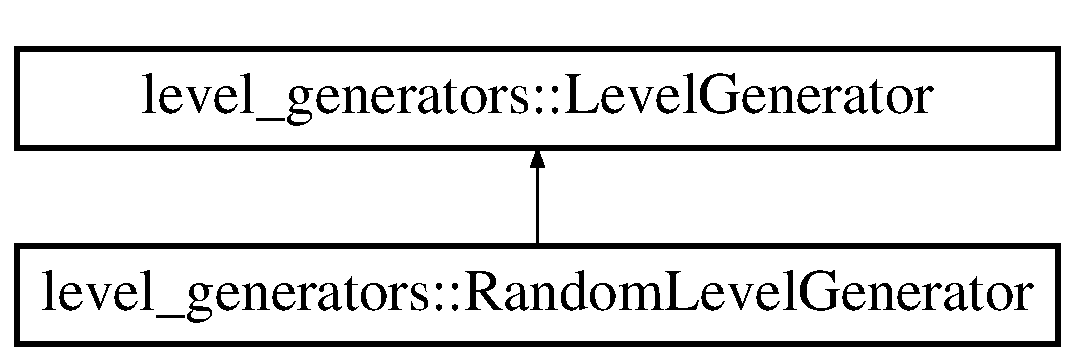
\includegraphics[height=2.000000cm]{classlevel__generators_1_1_level_generator}
\end{center}
\end{figure}
\subsection*{Public Member Functions}
\begin{DoxyCompactItemize}
\item 
\hyperlink{classlevel__generators_1_1_level_generator_a09a0e5fd9fbc3163228139d9b44bdf83}{Level\+Generator} (\hyperlink{class_entity_system}{Entity\+System} \&, tdt\+::uint)
\begin{DoxyCompactList}\small\item\em Constructor. \end{DoxyCompactList}\item 
virtual \hyperlink{classlevel__generators_1_1_level_generator_aba8153552145b2d710b1f6996bdfb997}{$\sim$\+Level\+Generator} ()=default
\begin{DoxyCompactList}\small\item\em Destructor. \end{DoxyCompactList}\item 
virtual void \hyperlink{classlevel__generators_1_1_level_generator_af5c177ea2e5b14b983c47c8c169c5ac7}{generate} (tdt\+::uint, tdt\+::uint, \hyperlink{class_wave_system}{Wave\+System} \&)=0
\begin{DoxyCompactList}\small\item\em Generates a level with the given dimensions. \end{DoxyCompactList}\end{DoxyCompactItemize}
\subsection*{Protected Attributes}
\begin{DoxyCompactItemize}
\item 
\hyperlink{class_entity_system}{Entity\+System} \& \hyperlink{classlevel__generators_1_1_level_generator_a9b50a95692ffc51ea52405a4058e50e8}{entities\+\_\+}
\begin{DoxyCompactList}\small\item\em Entity system that contains the level\textquotesingle{}s entities. \end{DoxyCompactList}\item 
tdt\+::uint \hyperlink{classlevel__generators_1_1_level_generator_a767d15a62998cb68c8576df073d4e891}{cycles\+\_\+}
\begin{DoxyCompactList}\small\item\em Number of cycles done while generating the world. \end{DoxyCompactList}\end{DoxyCompactItemize}


\subsection{Detailed Description}
Abstract parent class of all level generators, allows for different level generators used to create levels with minimal effort. 

Definition at line 20 of file Level\+Generators.\+hpp.



\subsection{Constructor \& Destructor Documentation}
\index{level\+\_\+generators\+::\+Level\+Generator@{level\+\_\+generators\+::\+Level\+Generator}!Level\+Generator@{Level\+Generator}}
\index{Level\+Generator@{Level\+Generator}!level\+\_\+generators\+::\+Level\+Generator@{level\+\_\+generators\+::\+Level\+Generator}}
\subsubsection[{\texorpdfstring{Level\+Generator(\+Entity\+System \&, tdt\+::uint)}{LevelGenerator(EntitySystem &, tdt::uint)}}]{\setlength{\rightskip}{0pt plus 5cm}level\+\_\+generators\+::\+Level\+Generator\+::\+Level\+Generator (
\begin{DoxyParamCaption}
\item[{{\bf Entity\+System} \&}]{ents, }
\item[{tdt\+::uint}]{c}
\end{DoxyParamCaption}
)}\hypertarget{classlevel__generators_1_1_level_generator_a09a0e5fd9fbc3163228139d9b44bdf83}{}\label{classlevel__generators_1_1_level_generator_a09a0e5fd9fbc3163228139d9b44bdf83}


Constructor. 


\begin{DoxyParams}{Parameters}
{\em Entity} & system that contains the level\textquotesingle{}s entities. \\
\hline
{\em Number} & of iterations done while generating. \\
\hline
\end{DoxyParams}


Definition at line 10 of file Level\+Generators.\+cpp.

\index{level\+\_\+generators\+::\+Level\+Generator@{level\+\_\+generators\+::\+Level\+Generator}!````~Level\+Generator@{$\sim$\+Level\+Generator}}
\index{````~Level\+Generator@{$\sim$\+Level\+Generator}!level\+\_\+generators\+::\+Level\+Generator@{level\+\_\+generators\+::\+Level\+Generator}}
\subsubsection[{\texorpdfstring{$\sim$\+Level\+Generator()=default}{~LevelGenerator()=default}}]{\setlength{\rightskip}{0pt plus 5cm}virtual level\+\_\+generators\+::\+Level\+Generator\+::$\sim$\+Level\+Generator (
\begin{DoxyParamCaption}
{}
\end{DoxyParamCaption}
)\hspace{0.3cm}{\ttfamily [virtual]}, {\ttfamily [default]}}\hypertarget{classlevel__generators_1_1_level_generator_aba8153552145b2d710b1f6996bdfb997}{}\label{classlevel__generators_1_1_level_generator_aba8153552145b2d710b1f6996bdfb997}


Destructor. 



\subsection{Member Function Documentation}
\index{level\+\_\+generators\+::\+Level\+Generator@{level\+\_\+generators\+::\+Level\+Generator}!generate@{generate}}
\index{generate@{generate}!level\+\_\+generators\+::\+Level\+Generator@{level\+\_\+generators\+::\+Level\+Generator}}
\subsubsection[{\texorpdfstring{generate(tdt\+::uint, tdt\+::uint, Wave\+System \&)=0}{generate(tdt::uint, tdt::uint, WaveSystem &)=0}}]{\setlength{\rightskip}{0pt plus 5cm}virtual void level\+\_\+generators\+::\+Level\+Generator\+::generate (
\begin{DoxyParamCaption}
\item[{tdt\+::uint}]{, }
\item[{tdt\+::uint}]{, }
\item[{{\bf Wave\+System} \&}]{}
\end{DoxyParamCaption}
)\hspace{0.3cm}{\ttfamily [pure virtual]}}\hypertarget{classlevel__generators_1_1_level_generator_af5c177ea2e5b14b983c47c8c169c5ac7}{}\label{classlevel__generators_1_1_level_generator_af5c177ea2e5b14b983c47c8c169c5ac7}


Generates a level with the given dimensions. 


\begin{DoxyParams}{Parameters}
{\em Width} & of the level. \\
\hline
{\em Height} & of the level. \\
\hline
{\em Wave} & system that will have it\textquotesingle{}s spawn nodes set. \\
\hline
\end{DoxyParams}


Implemented in \hyperlink{classlevel__generators_1_1_random_level_generator_a085098cd10565bd3f9c6b13f68fcc1cb}{level\+\_\+generators\+::\+Random\+Level\+Generator}.



\subsection{Member Data Documentation}
\index{level\+\_\+generators\+::\+Level\+Generator@{level\+\_\+generators\+::\+Level\+Generator}!cycles\+\_\+@{cycles\+\_\+}}
\index{cycles\+\_\+@{cycles\+\_\+}!level\+\_\+generators\+::\+Level\+Generator@{level\+\_\+generators\+::\+Level\+Generator}}
\subsubsection[{\texorpdfstring{cycles\+\_\+}{cycles_}}]{\setlength{\rightskip}{0pt plus 5cm}tdt\+::uint level\+\_\+generators\+::\+Level\+Generator\+::cycles\+\_\+\hspace{0.3cm}{\ttfamily [protected]}}\hypertarget{classlevel__generators_1_1_level_generator_a767d15a62998cb68c8576df073d4e891}{}\label{classlevel__generators_1_1_level_generator_a767d15a62998cb68c8576df073d4e891}


Number of cycles done while generating the world. 



Definition at line 52 of file Level\+Generators.\+hpp.

\index{level\+\_\+generators\+::\+Level\+Generator@{level\+\_\+generators\+::\+Level\+Generator}!entities\+\_\+@{entities\+\_\+}}
\index{entities\+\_\+@{entities\+\_\+}!level\+\_\+generators\+::\+Level\+Generator@{level\+\_\+generators\+::\+Level\+Generator}}
\subsubsection[{\texorpdfstring{entities\+\_\+}{entities_}}]{\setlength{\rightskip}{0pt plus 5cm}{\bf Entity\+System}\& level\+\_\+generators\+::\+Level\+Generator\+::entities\+\_\+\hspace{0.3cm}{\ttfamily [protected]}}\hypertarget{classlevel__generators_1_1_level_generator_a9b50a95692ffc51ea52405a4058e50e8}{}\label{classlevel__generators_1_1_level_generator_a9b50a95692ffc51ea52405a4058e50e8}


Entity system that contains the level\textquotesingle{}s entities. 



Definition at line 47 of file Level\+Generators.\+hpp.



The documentation for this class was generated from the following files\+:\begin{DoxyCompactItemize}
\item 
tools/Level\+Generators.\+hpp\item 
tools/Level\+Generators.\+cpp\end{DoxyCompactItemize}

\hypertarget{struct_light_component}{}\section{Light\+Component Struct Reference}
\label{struct_light_component}\index{Light\+Component@{Light\+Component}}


Allows an entity to emit light to it\textquotesingle{}s surrounding area.  




{\ttfamily \#include $<$Components.\+hpp$>$}

\subsection*{Public Member Functions}
\begin{DoxyCompactItemize}
\item 
{\bfseries Light\+Component} (const \hyperlink{struct_light_component}{Light\+Component} \&)=default\hypertarget{struct_light_component_a179937f38c9f7a15b104ada3af8da472}{}\label{struct_light_component_a179937f38c9f7a15b104ada3af8da472}

\item 
{\bfseries Light\+Component} (\hyperlink{struct_light_component}{Light\+Component} \&\&)=default\hypertarget{struct_light_component_a95ea0325371c3ad95b0a567484419dd3}{}\label{struct_light_component_a95ea0325371c3ad95b0a567484419dd3}

\item 
\hyperlink{struct_light_component}{Light\+Component} \& {\bfseries operator=} (const \hyperlink{struct_light_component}{Light\+Component} \&)=default\hypertarget{struct_light_component_add309e16a4d282952e52a0d354f5c290}{}\label{struct_light_component_add309e16a4d282952e52a0d354f5c290}

\item 
\hyperlink{struct_light_component}{Light\+Component} \& {\bfseries operator=} (\hyperlink{struct_light_component}{Light\+Component} \&\&)=default\hypertarget{struct_light_component_af03a690e9e9b70a34f7dbda80d07f8b7}{}\label{struct_light_component_af03a690e9e9b70a34f7dbda80d07f8b7}

\end{DoxyCompactItemize}
\subsection*{Public Attributes}
\begin{DoxyCompactItemize}
\item 
Ogre\+::\+Scene\+Node $\ast$ {\bfseries node}\hypertarget{struct_light_component_af0376f045845ff28decf09fc2c89064a}{}\label{struct_light_component_af0376f045845ff28decf09fc2c89064a}

\item 
Ogre\+::\+Light $\ast$ {\bfseries light}\hypertarget{struct_light_component_a24973661f3fd0b9577308c8991999ff3}{}\label{struct_light_component_a24973661f3fd0b9577308c8991999ff3}

\end{DoxyCompactItemize}
\subsection*{Static Public Attributes}
\begin{DoxyCompactItemize}
\item 
static constexpr int {\bfseries type} = 36\hypertarget{struct_light_component_ab5bbdfb4bf129d19b7e4aa942dfb264b}{}\label{struct_light_component_ab5bbdfb4bf129d19b7e4aa942dfb264b}

\end{DoxyCompactItemize}


\subsection{Detailed Description}
Allows an entity to emit light to it\textquotesingle{}s surrounding area. 

Definition at line 841 of file Components.\+hpp.



The documentation for this struct was generated from the following file\+:\begin{DoxyCompactItemize}
\item 
Components.\+hpp\end{DoxyCompactItemize}

\hypertarget{struct_limited_life_span_component}{}\section{Limited\+Life\+Span\+Component Struct Reference}
\label{struct_limited_life_span_component}\index{Limited\+Life\+Span\+Component@{Limited\+Life\+Span\+Component}}


Allows to create entities that are automatically killed (summons) after a certain amount of time has passed (lifespan).  




{\ttfamily \#include $<$Components.\+hpp$>$}

\subsection*{Public Member Functions}
\begin{DoxyCompactItemize}
\item 
{\bfseries Limited\+Life\+Span\+Component} (tdt\+::real max=0.f)\hypertarget{struct_limited_life_span_component_a41a11ccc2b41be1c2ec9aec57fc70e3e}{}\label{struct_limited_life_span_component_a41a11ccc2b41be1c2ec9aec57fc70e3e}

\item 
{\bfseries Limited\+Life\+Span\+Component} (const \hyperlink{struct_limited_life_span_component}{Limited\+Life\+Span\+Component} \&)=default\hypertarget{struct_limited_life_span_component_af9b148d4d3335fe27f79d2313210f2b2}{}\label{struct_limited_life_span_component_af9b148d4d3335fe27f79d2313210f2b2}

\item 
{\bfseries Limited\+Life\+Span\+Component} (\hyperlink{struct_limited_life_span_component}{Limited\+Life\+Span\+Component} \&\&)=default\hypertarget{struct_limited_life_span_component_aab4f274ec695cf686ed97b0fe9d59945}{}\label{struct_limited_life_span_component_aab4f274ec695cf686ed97b0fe9d59945}

\item 
\hyperlink{struct_limited_life_span_component}{Limited\+Life\+Span\+Component} \& {\bfseries operator=} (const \hyperlink{struct_limited_life_span_component}{Limited\+Life\+Span\+Component} \&)=default\hypertarget{struct_limited_life_span_component_a731d9304fd1e0bf7ab45df6b4b2d347c}{}\label{struct_limited_life_span_component_a731d9304fd1e0bf7ab45df6b4b2d347c}

\item 
\hyperlink{struct_limited_life_span_component}{Limited\+Life\+Span\+Component} \& {\bfseries operator=} (\hyperlink{struct_limited_life_span_component}{Limited\+Life\+Span\+Component} \&\&)=default\hypertarget{struct_limited_life_span_component_ab1d4ee3212d6b080e5d049bdd963de12}{}\label{struct_limited_life_span_component_ab1d4ee3212d6b080e5d049bdd963de12}

\end{DoxyCompactItemize}
\subsection*{Public Attributes}
\begin{DoxyCompactItemize}
\item 
tdt\+::real {\bfseries curr\+\_\+time}\hypertarget{struct_limited_life_span_component_ab862d54c222a65770983371d9c5c64f8}{}\label{struct_limited_life_span_component_ab862d54c222a65770983371d9c5c64f8}

\item 
tdt\+::real {\bfseries max\+\_\+time}\hypertarget{struct_limited_life_span_component_afa5a006f8233d28d9249bc81dfca4fcd}{}\label{struct_limited_life_span_component_afa5a006f8233d28d9249bc81dfca4fcd}

\end{DoxyCompactItemize}
\subsection*{Static Public Attributes}
\begin{DoxyCompactItemize}
\item 
static constexpr int {\bfseries type} = 33\hypertarget{struct_limited_life_span_component_a36c15b9b5393ecfb0590a06eaf09a301}{}\label{struct_limited_life_span_component_a36c15b9b5393ecfb0590a06eaf09a301}

\end{DoxyCompactItemize}


\subsection{Detailed Description}
Allows to create entities that are automatically killed (summons) after a certain amount of time has passed (lifespan). 

Definition at line 783 of file Components.\+hpp.



The documentation for this struct was generated from the following file\+:\begin{DoxyCompactItemize}
\item 
Components.\+hpp\end{DoxyCompactItemize}

\hypertarget{structutil_1_1effect_1_1_l_o_w_e_r___s_p_e_e_d___e_f_f_e_c_t}{}\section{util\+:\+:effect\+:\+:L\+O\+W\+E\+R\+\_\+\+S\+P\+E\+E\+D\+\_\+\+E\+F\+F\+E\+CT Struct Reference}
\label{structutil_1_1effect_1_1_l_o_w_e_r___s_p_e_e_d___e_f_f_e_c_t}\index{util\+::effect\+::\+L\+O\+W\+E\+R\+\_\+\+S\+P\+E\+E\+D\+\_\+\+E\+F\+F\+E\+CT@{util\+::effect\+::\+L\+O\+W\+E\+R\+\_\+\+S\+P\+E\+E\+D\+\_\+\+E\+F\+F\+E\+CT}}


Halves the speed of the entity it\textquotesingle{}s called on for a given time period.  




{\ttfamily \#include $<$Effects.\+hpp$>$}

\subsection*{Public Member Functions}
\begin{DoxyCompactItemize}
\item 
\hyperlink{structutil_1_1effect_1_1_l_o_w_e_r___s_p_e_e_d___e_f_f_e_c_t_a229ec35de341edfbe481c91c1aa4b422}{L\+O\+W\+E\+R\+\_\+\+S\+P\+E\+E\+D\+\_\+\+E\+F\+F\+E\+CT} (\hyperlink{class_entity_system}{Entity\+System} \&, tdt\+::real)
\begin{DoxyCompactList}\small\item\em Constructor. \end{DoxyCompactList}\item 
\hyperlink{structutil_1_1effect_1_1_l_o_w_e_r___s_p_e_e_d___e_f_f_e_c_t_a3051d8bdb4e2cb3d5949fd3b7c543080}{$\sim$\+L\+O\+W\+E\+R\+\_\+\+S\+P\+E\+E\+D\+\_\+\+E\+F\+F\+E\+CT} ()=default
\begin{DoxyCompactList}\small\item\em Destructor. \end{DoxyCompactList}\item 
void \hyperlink{structutil_1_1effect_1_1_l_o_w_e_r___s_p_e_e_d___e_f_f_e_c_t_a895b93602a1f6cd53b1edc3438a0d25f}{operator()} (tdt\+::uint)
\begin{DoxyCompactList}\small\item\em Halves the speed of a given entity. \end{DoxyCompactList}\end{DoxyCompactItemize}
\subsection*{Private Attributes}
\begin{DoxyCompactItemize}
\item 
\hyperlink{class_entity_system}{Entity\+System} \& \hyperlink{structutil_1_1effect_1_1_l_o_w_e_r___s_p_e_e_d___e_f_f_e_c_t_a139300dc0d6a1057cdec73bc4f984ad2}{entities\+\_\+}
\begin{DoxyCompactList}\small\item\em Entity system containing the entities this effect will be called on. \end{DoxyCompactList}\item 
tdt\+::real \hyperlink{structutil_1_1effect_1_1_l_o_w_e_r___s_p_e_e_d___e_f_f_e_c_t_a1de62813271d93d454f2fa3faba8ebdc}{time\+\_\+}
\begin{DoxyCompactList}\small\item\em The time period that has to pass before the speed of the affected entities gets restored. \end{DoxyCompactList}\end{DoxyCompactItemize}


\subsection{Detailed Description}
Halves the speed of the entity it\textquotesingle{}s called on for a given time period. 

Definition at line 93 of file Effects.\+hpp.



\subsection{Constructor \& Destructor Documentation}
\index{util\+::effect\+::\+L\+O\+W\+E\+R\+\_\+\+S\+P\+E\+E\+D\+\_\+\+E\+F\+F\+E\+CT@{util\+::effect\+::\+L\+O\+W\+E\+R\+\_\+\+S\+P\+E\+E\+D\+\_\+\+E\+F\+F\+E\+CT}!L\+O\+W\+E\+R\+\_\+\+S\+P\+E\+E\+D\+\_\+\+E\+F\+F\+E\+CT@{L\+O\+W\+E\+R\+\_\+\+S\+P\+E\+E\+D\+\_\+\+E\+F\+F\+E\+CT}}
\index{L\+O\+W\+E\+R\+\_\+\+S\+P\+E\+E\+D\+\_\+\+E\+F\+F\+E\+CT@{L\+O\+W\+E\+R\+\_\+\+S\+P\+E\+E\+D\+\_\+\+E\+F\+F\+E\+CT}!util\+::effect\+::\+L\+O\+W\+E\+R\+\_\+\+S\+P\+E\+E\+D\+\_\+\+E\+F\+F\+E\+CT@{util\+::effect\+::\+L\+O\+W\+E\+R\+\_\+\+S\+P\+E\+E\+D\+\_\+\+E\+F\+F\+E\+CT}}
\subsubsection[{\texorpdfstring{L\+O\+W\+E\+R\+\_\+\+S\+P\+E\+E\+D\+\_\+\+E\+F\+F\+E\+C\+T(\+Entity\+System \&, tdt\+::real)}{LOWER_SPEED_EFFECT(EntitySystem &, tdt::real)}}]{\setlength{\rightskip}{0pt plus 5cm}util\+::effect\+::\+L\+O\+W\+E\+R\+\_\+\+S\+P\+E\+E\+D\+\_\+\+E\+F\+F\+E\+C\+T\+::\+L\+O\+W\+E\+R\+\_\+\+S\+P\+E\+E\+D\+\_\+\+E\+F\+F\+E\+CT (
\begin{DoxyParamCaption}
\item[{{\bf Entity\+System} \&}]{ents, }
\item[{tdt\+::real}]{time}
\end{DoxyParamCaption}
)}\hypertarget{structutil_1_1effect_1_1_l_o_w_e_r___s_p_e_e_d___e_f_f_e_c_t_a229ec35de341edfbe481c91c1aa4b422}{}\label{structutil_1_1effect_1_1_l_o_w_e_r___s_p_e_e_d___e_f_f_e_c_t_a229ec35de341edfbe481c91c1aa4b422}


Constructor. 


\begin{DoxyParams}{Parameters}
{\em Entity} & system containing the entities this effect will be called on. \\
\hline
{\em The} & time period before the speed is restored. \\
\hline
\end{DoxyParams}


Definition at line 25 of file Effects.\+cpp.

\index{util\+::effect\+::\+L\+O\+W\+E\+R\+\_\+\+S\+P\+E\+E\+D\+\_\+\+E\+F\+F\+E\+CT@{util\+::effect\+::\+L\+O\+W\+E\+R\+\_\+\+S\+P\+E\+E\+D\+\_\+\+E\+F\+F\+E\+CT}!````~L\+O\+W\+E\+R\+\_\+\+S\+P\+E\+E\+D\+\_\+\+E\+F\+F\+E\+CT@{$\sim$\+L\+O\+W\+E\+R\+\_\+\+S\+P\+E\+E\+D\+\_\+\+E\+F\+F\+E\+CT}}
\index{````~L\+O\+W\+E\+R\+\_\+\+S\+P\+E\+E\+D\+\_\+\+E\+F\+F\+E\+CT@{$\sim$\+L\+O\+W\+E\+R\+\_\+\+S\+P\+E\+E\+D\+\_\+\+E\+F\+F\+E\+CT}!util\+::effect\+::\+L\+O\+W\+E\+R\+\_\+\+S\+P\+E\+E\+D\+\_\+\+E\+F\+F\+E\+CT@{util\+::effect\+::\+L\+O\+W\+E\+R\+\_\+\+S\+P\+E\+E\+D\+\_\+\+E\+F\+F\+E\+CT}}
\subsubsection[{\texorpdfstring{$\sim$\+L\+O\+W\+E\+R\+\_\+\+S\+P\+E\+E\+D\+\_\+\+E\+F\+F\+E\+C\+T()=default}{~LOWER_SPEED_EFFECT()=default}}]{\setlength{\rightskip}{0pt plus 5cm}util\+::effect\+::\+L\+O\+W\+E\+R\+\_\+\+S\+P\+E\+E\+D\+\_\+\+E\+F\+F\+E\+C\+T\+::$\sim$\+L\+O\+W\+E\+R\+\_\+\+S\+P\+E\+E\+D\+\_\+\+E\+F\+F\+E\+CT (
\begin{DoxyParamCaption}
{}
\end{DoxyParamCaption}
)\hspace{0.3cm}{\ttfamily [default]}}\hypertarget{structutil_1_1effect_1_1_l_o_w_e_r___s_p_e_e_d___e_f_f_e_c_t_a3051d8bdb4e2cb3d5949fd3b7c543080}{}\label{structutil_1_1effect_1_1_l_o_w_e_r___s_p_e_e_d___e_f_f_e_c_t_a3051d8bdb4e2cb3d5949fd3b7c543080}


Destructor. 



\subsection{Member Function Documentation}
\index{util\+::effect\+::\+L\+O\+W\+E\+R\+\_\+\+S\+P\+E\+E\+D\+\_\+\+E\+F\+F\+E\+CT@{util\+::effect\+::\+L\+O\+W\+E\+R\+\_\+\+S\+P\+E\+E\+D\+\_\+\+E\+F\+F\+E\+CT}!operator()@{operator()}}
\index{operator()@{operator()}!util\+::effect\+::\+L\+O\+W\+E\+R\+\_\+\+S\+P\+E\+E\+D\+\_\+\+E\+F\+F\+E\+CT@{util\+::effect\+::\+L\+O\+W\+E\+R\+\_\+\+S\+P\+E\+E\+D\+\_\+\+E\+F\+F\+E\+CT}}
\subsubsection[{\texorpdfstring{operator()(tdt\+::uint)}{operator()(tdt::uint)}}]{\setlength{\rightskip}{0pt plus 5cm}void util\+::effect\+::\+L\+O\+W\+E\+R\+\_\+\+S\+P\+E\+E\+D\+\_\+\+E\+F\+F\+E\+C\+T\+::operator() (
\begin{DoxyParamCaption}
\item[{tdt\+::uint}]{id}
\end{DoxyParamCaption}
)}\hypertarget{structutil_1_1effect_1_1_l_o_w_e_r___s_p_e_e_d___e_f_f_e_c_t_a895b93602a1f6cd53b1edc3438a0d25f}{}\label{structutil_1_1effect_1_1_l_o_w_e_r___s_p_e_e_d___e_f_f_e_c_t_a895b93602a1f6cd53b1edc3438a0d25f}


Halves the speed of a given entity. 


\begin{DoxyParams}{Parameters}
{\em ID} & of the entity. \\
\hline
\end{DoxyParams}


Definition at line 29 of file Effects.\+cpp.



\subsection{Member Data Documentation}
\index{util\+::effect\+::\+L\+O\+W\+E\+R\+\_\+\+S\+P\+E\+E\+D\+\_\+\+E\+F\+F\+E\+CT@{util\+::effect\+::\+L\+O\+W\+E\+R\+\_\+\+S\+P\+E\+E\+D\+\_\+\+E\+F\+F\+E\+CT}!entities\+\_\+@{entities\+\_\+}}
\index{entities\+\_\+@{entities\+\_\+}!util\+::effect\+::\+L\+O\+W\+E\+R\+\_\+\+S\+P\+E\+E\+D\+\_\+\+E\+F\+F\+E\+CT@{util\+::effect\+::\+L\+O\+W\+E\+R\+\_\+\+S\+P\+E\+E\+D\+\_\+\+E\+F\+F\+E\+CT}}
\subsubsection[{\texorpdfstring{entities\+\_\+}{entities_}}]{\setlength{\rightskip}{0pt plus 5cm}{\bf Entity\+System}\& util\+::effect\+::\+L\+O\+W\+E\+R\+\_\+\+S\+P\+E\+E\+D\+\_\+\+E\+F\+F\+E\+C\+T\+::entities\+\_\+\hspace{0.3cm}{\ttfamily [private]}}\hypertarget{structutil_1_1effect_1_1_l_o_w_e_r___s_p_e_e_d___e_f_f_e_c_t_a139300dc0d6a1057cdec73bc4f984ad2}{}\label{structutil_1_1effect_1_1_l_o_w_e_r___s_p_e_e_d___e_f_f_e_c_t_a139300dc0d6a1057cdec73bc4f984ad2}


Entity system containing the entities this effect will be called on. 



Definition at line 119 of file Effects.\+hpp.

\index{util\+::effect\+::\+L\+O\+W\+E\+R\+\_\+\+S\+P\+E\+E\+D\+\_\+\+E\+F\+F\+E\+CT@{util\+::effect\+::\+L\+O\+W\+E\+R\+\_\+\+S\+P\+E\+E\+D\+\_\+\+E\+F\+F\+E\+CT}!time\+\_\+@{time\+\_\+}}
\index{time\+\_\+@{time\+\_\+}!util\+::effect\+::\+L\+O\+W\+E\+R\+\_\+\+S\+P\+E\+E\+D\+\_\+\+E\+F\+F\+E\+CT@{util\+::effect\+::\+L\+O\+W\+E\+R\+\_\+\+S\+P\+E\+E\+D\+\_\+\+E\+F\+F\+E\+CT}}
\subsubsection[{\texorpdfstring{time\+\_\+}{time_}}]{\setlength{\rightskip}{0pt plus 5cm}tdt\+::real util\+::effect\+::\+L\+O\+W\+E\+R\+\_\+\+S\+P\+E\+E\+D\+\_\+\+E\+F\+F\+E\+C\+T\+::time\+\_\+\hspace{0.3cm}{\ttfamily [private]}}\hypertarget{structutil_1_1effect_1_1_l_o_w_e_r___s_p_e_e_d___e_f_f_e_c_t_a1de62813271d93d454f2fa3faba8ebdc}{}\label{structutil_1_1effect_1_1_l_o_w_e_r___s_p_e_e_d___e_f_f_e_c_t_a1de62813271d93d454f2fa3faba8ebdc}


The time period that has to pass before the speed of the affected entities gets restored. 



Definition at line 125 of file Effects.\+hpp.



The documentation for this struct was generated from the following files\+:\begin{DoxyCompactItemize}
\item 
tools/Effects.\+hpp\item 
tools/Effects.\+cpp\end{DoxyCompactItemize}

\hypertarget{class_lua_interface}{}\section{Lua\+Interface Class Reference}
\label{class_lua_interface}\index{Lua\+Interface@{Lua\+Interface}}


Class that creates an interface between engine (C++) and logic (Lua) code.  




{\ttfamily \#include $<$Lua\+Interface.\+hpp$>$}

\subsection*{Public Member Functions}
\begin{DoxyCompactItemize}
\item 
\hyperlink{class_lua_interface_a10d0df765a9d8c8282c18a5ce43d0f9e}{Lua\+Interface} ()=delete
\begin{DoxyCompactList}\small\item\em This is a static class, so all constructors are deleted. \end{DoxyCompactList}\item 
{\bfseries Lua\+Interface} (const \hyperlink{class_lua_interface}{Lua\+Interface} \&)=delete\hypertarget{class_lua_interface_a925145fb427267abcff404742e1df805}{}\label{class_lua_interface_a925145fb427267abcff404742e1df805}

\item 
{\bfseries Lua\+Interface} (\hyperlink{class_lua_interface}{Lua\+Interface} \&\&)=delete\hypertarget{class_lua_interface_ad7b50588c30ea8c133539efd4f532180}{}\label{class_lua_interface_ad7b50588c30ea8c133539efd4f532180}

\end{DoxyCompactItemize}
\subsection*{Static Public Member Functions}
\begin{DoxyCompactItemize}
\item 
static void \hyperlink{class_lua_interface_ac9fa6b609503a1db2c44b7f27f8d1090}{init} (\hyperlink{class_game}{Game} $\ast$)
\begin{DoxyCompactList}\small\item\em Sets the lua\+\_\+this pointer and registers all C++ A\+PI functions to Lua. \end{DoxyCompactList}\end{DoxyCompactItemize}
\subsection*{Static Private Member Functions}
\begin{DoxyCompactItemize}
\item 
static int \hyperlink{class_lua_interface_aac8cc7f5beeb8ffe8d637abc7a1d3600}{lua\+\_\+get\+\_\+avg\+\_\+fps} (lpp\+::\+Script\+::state)
\item 
static int {\bfseries lua\+\_\+get\+\_\+fps} (lpp\+::\+Script\+::state)\hypertarget{class_lua_interface_a29f3c1ffa0a902adac4e67d3385d5af4}{}\label{class_lua_interface_a29f3c1ffa0a902adac4e67d3385d5af4}

\item 
static int {\bfseries lua\+\_\+print} (lpp\+::\+Script\+::state)\hypertarget{class_lua_interface_a51e679ea9a576d2aeefedd1c959f45d7}{}\label{class_lua_interface_a51e679ea9a576d2aeefedd1c959f45d7}

\item 
static int {\bfseries lua\+\_\+set\+\_\+game\+\_\+state} (lpp\+::\+Script\+::state)\hypertarget{class_lua_interface_a5aa5fff6b89dd6be1beac175957eb80d}{}\label{class_lua_interface_a5aa5fff6b89dd6be1beac175957eb80d}

\item 
static int {\bfseries lua\+\_\+toggle\+\_\+bounding\+\_\+boxes} (lpp\+::\+Script\+::state)\hypertarget{class_lua_interface_ac37363a7902485c77456c3272c3d812d}{}\label{class_lua_interface_ac37363a7902485c77456c3272c3d812d}

\item 
static int {\bfseries lua\+\_\+toggle\+\_\+camera\+\_\+free\+\_\+mode} (lpp\+::\+Script\+::state)\hypertarget{class_lua_interface_af4efc25e6844f768fa5b0334c8f54d40}{}\label{class_lua_interface_af4efc25e6844f768fa5b0334c8f54d40}

\item 
static int {\bfseries lua\+\_\+toggle\+\_\+entity\+\_\+creator} (lpp\+::\+Script\+::state)\hypertarget{class_lua_interface_ab9590bfdd7bdd79dc84295ce4c1e4bd9}{}\label{class_lua_interface_ab9590bfdd7bdd79dc84295ce4c1e4bd9}

\item 
static int {\bfseries lua\+\_\+list\+\_\+selected} (lpp\+::\+Script\+::state)\hypertarget{class_lua_interface_a27826f52870ace0f8a7fb2e94815ed14}{}\label{class_lua_interface_a27826f52870ace0f8a7fb2e94815ed14}

\item 
static int {\bfseries lua\+\_\+destroy\+\_\+selected} (lpp\+::\+Script\+::state)\hypertarget{class_lua_interface_ae67e86128e80404fa6a4876db465ae75}{}\label{class_lua_interface_ae67e86128e80404fa6a4876db465ae75}

\item 
static int {\bfseries lua\+\_\+kill\+\_\+selected} (lpp\+::\+Script\+::state)\hypertarget{class_lua_interface_ad3ef59891e0aba8fb768ae372c45742d}{}\label{class_lua_interface_ad3ef59891e0aba8fb768ae372c45742d}

\item 
static int {\bfseries lua\+\_\+list\+\_\+components\+\_\+of} (lpp\+::\+Script\+::state)\hypertarget{class_lua_interface_a542d175e198d07aedc7138f898bc83fd}{}\label{class_lua_interface_a542d175e198d07aedc7138f898bc83fd}

\item 
static int {\bfseries lua\+\_\+load} (lpp\+::\+Script\+::state)\hypertarget{class_lua_interface_a7deaf3615eb31fd09a1ddacd461ee93a}{}\label{class_lua_interface_a7deaf3615eb31fd09a1ddacd461ee93a}

\item 
static int {\bfseries lua\+\_\+reload\+\_\+all} (lpp\+::\+Script\+::state)\hypertarget{class_lua_interface_a708acacbb59eb74133655687fb91fb7a}{}\label{class_lua_interface_a708acacbb59eb74133655687fb91fb7a}

\item 
static int {\bfseries lua\+\_\+save\+\_\+game} (lpp\+::\+Script\+::state)\hypertarget{class_lua_interface_a7f7a0ba475425b5b58e95e1618c1bda7}{}\label{class_lua_interface_a7f7a0ba475425b5b58e95e1618c1bda7}

\item 
static int {\bfseries lua\+\_\+load\+\_\+game} (lpp\+::\+Script\+::state)\hypertarget{class_lua_interface_a57b4d9d83f74827e07aa1e32c7483dc4}{}\label{class_lua_interface_a57b4d9d83f74827e07aa1e32c7483dc4}

\item 
static int {\bfseries lua\+\_\+get\+\_\+cursor\+\_\+position} (lpp\+::\+Script\+::state)\hypertarget{class_lua_interface_aa6ce840b4264593baa5567a9eaa9a9dd}{}\label{class_lua_interface_aa6ce840b4264593baa5567a9eaa9a9dd}

\item 
static int {\bfseries lua\+\_\+can\+\_\+place\+\_\+when\+\_\+game\+\_\+paused} (lpp\+::\+Script\+::state)\hypertarget{class_lua_interface_a2ea3dfb29a9cf844908713e2a0cec5d9}{}\label{class_lua_interface_a2ea3dfb29a9cf844908713e2a0cec5d9}

\item 
static int {\bfseries lua\+\_\+toggle\+\_\+placing\+\_\+when\+\_\+game\+\_\+paused} (lpp\+::\+Script\+::state)\hypertarget{class_lua_interface_a59a4852b61dd0af2665185bca1755f59}{}\label{class_lua_interface_a59a4852b61dd0af2665185bca1755f59}

\item 
static int {\bfseries lua\+\_\+new\+\_\+game} (lpp\+::\+Script\+::state)\hypertarget{class_lua_interface_a75ef98d36684c3eb6741ebc1f9cf8dec}{}\label{class_lua_interface_a75ef98d36684c3eb6741ebc1f9cf8dec}

\item 
static int {\bfseries lua\+\_\+create\+\_\+empty\+\_\+level} (lpp\+::\+Script\+::state)\hypertarget{class_lua_interface_a32b89eaa09197ca9783b4ba7a7358b0a}{}\label{class_lua_interface_a32b89eaa09197ca9783b4ba7a7358b0a}

\item 
static int {\bfseries lua\+\_\+reset\+\_\+unlocks} (lpp\+::\+Script\+::state)\hypertarget{class_lua_interface_ac3cef8a0fa0e32992f909511ff4ace76}{}\label{class_lua_interface_ac3cef8a0fa0e32992f909511ff4ace76}

\item 
static int {\bfseries lua\+\_\+get\+\_\+random} (lpp\+::\+Script\+::state)\hypertarget{class_lua_interface_af86a3e370385e95f7da5e92996b511f6}{}\label{class_lua_interface_af86a3e370385e95f7da5e92996b511f6}

\item 
static int {\bfseries lua\+\_\+set\+\_\+key\+\_\+bind} (lpp\+::\+Script\+::state)\hypertarget{class_lua_interface_a29eade8a630409d8a905d45613ad154e}{}\label{class_lua_interface_a29eade8a630409d8a905d45613ad154e}

\item 
static int {\bfseries lua\+\_\+get\+\_\+first\+\_\+selected} (lpp\+::\+Script\+::state)\hypertarget{class_lua_interface_a7f95a569cf02e3e8af912f7467792b2e}{}\label{class_lua_interface_a7f95a569cf02e3e8af912f7467792b2e}

\item 
static int {\bfseries lua\+\_\+get\+\_\+enemies} (lpp\+::\+Script\+::state)\hypertarget{class_lua_interface_ad16b0e337997f766ca7bbd1aac579379}{}\label{class_lua_interface_ad16b0e337997f766ca7bbd1aac579379}

\item 
static int {\bfseries lua\+\_\+get\+\_\+friends} (lpp\+::\+Script\+::state)\hypertarget{class_lua_interface_a3a7cae862d7bbd8b50673c64aeb1a351}{}\label{class_lua_interface_a3a7cae862d7bbd8b50673c64aeb1a351}

\item 
static int {\bfseries lua\+\_\+set\+\_\+throne\+\_\+id} (lpp\+::\+Script\+::state)\hypertarget{class_lua_interface_a32c2aa6a6af54e6aa68fccb798b3e74f}{}\label{class_lua_interface_a32c2aa6a6af54e6aa68fccb798b3e74f}

\item 
static int {\bfseries lua\+\_\+get\+\_\+throne\+\_\+id} (lpp\+::\+Script\+::state)\hypertarget{class_lua_interface_a9eaf35a68a3087989121f36474d4b0fe}{}\label{class_lua_interface_a9eaf35a68a3087989121f36474d4b0fe}

\item 
static int {\bfseries lua\+\_\+command\+\_\+to\+\_\+mine} (lpp\+::\+Script\+::state)\hypertarget{class_lua_interface_a3cd1be7ff7b06294f6a66efbfeee7071}{}\label{class_lua_interface_a3cd1be7ff7b06294f6a66efbfeee7071}

\item 
static int {\bfseries lua\+\_\+command\+\_\+to\+\_\+attack} (lpp\+::\+Script\+::state)\hypertarget{class_lua_interface_a1fb505ff6b59e9bfa5ab87807d75bae6}{}\label{class_lua_interface_a1fb505ff6b59e9bfa5ab87807d75bae6}

\item 
static int {\bfseries lua\+\_\+command\+\_\+to\+\_\+reposition} (lpp\+::\+Script\+::state)\hypertarget{class_lua_interface_ad520a98ea394025d5332210a9c3e1471}{}\label{class_lua_interface_ad520a98ea394025d5332210a9c3e1471}

\item 
static int {\bfseries lua\+\_\+command\+\_\+to\+\_\+return\+\_\+gold} (lpp\+::\+Script\+::state)\hypertarget{class_lua_interface_a27d683ce4a5b270413c99344a4078c40}{}\label{class_lua_interface_a27d683ce4a5b270413c99344a4078c40}

\item 
static int {\bfseries lua\+\_\+command\+\_\+to\+\_\+fall\+\_\+back} (lpp\+::\+Script\+::state)\hypertarget{class_lua_interface_aa22a3fb04f40b166b45b930825a90bbc}{}\label{class_lua_interface_aa22a3fb04f40b166b45b930825a90bbc}

\item 
static int {\bfseries lua\+\_\+get\+\_\+enum\+\_\+direction} (lpp\+::\+Script\+::state)\hypertarget{class_lua_interface_a983b36d571294e832c237119daa65187}{}\label{class_lua_interface_a983b36d571294e832c237119daa65187}

\item 
static int {\bfseries lua\+\_\+get\+\_\+node\+\_\+in\+\_\+dir} (lpp\+::\+Script\+::state)\hypertarget{class_lua_interface_a83d576d5113c1cf8cc0f9e298962e3d1}{}\label{class_lua_interface_a83d576d5113c1cf8cc0f9e298962e3d1}

\item 
static int {\bfseries lua\+\_\+set\+\_\+mesh} (lpp\+::\+Script\+::state)\hypertarget{class_lua_interface_abef84137aa944683616cd1e96db814de}{}\label{class_lua_interface_abef84137aa944683616cd1e96db814de}

\item 
static int {\bfseries lua\+\_\+set\+\_\+material} (lpp\+::\+Script\+::state)\hypertarget{class_lua_interface_a1d34ae0354dc0003a043524188f1b7fd}{}\label{class_lua_interface_a1d34ae0354dc0003a043524188f1b7fd}

\item 
static int {\bfseries lua\+\_\+set\+\_\+visible} (lpp\+::\+Script\+::state)\hypertarget{class_lua_interface_a62f2408b5220f1430583ea24c66795dc}{}\label{class_lua_interface_a62f2408b5220f1430583ea24c66795dc}

\item 
static int {\bfseries lua\+\_\+set\+\_\+manual\+\_\+scaling} (lpp\+::\+Script\+::state)\hypertarget{class_lua_interface_aaabaca1e0e0e47bdfd46fcd9e36856ba}{}\label{class_lua_interface_aaabaca1e0e0e47bdfd46fcd9e36856ba}

\item 
static int {\bfseries lua\+\_\+set\+\_\+scale} (lpp\+::\+Script\+::state)\hypertarget{class_lua_interface_a4360b8ff9e75c3a7e92ae9f9a1a2e1b5}{}\label{class_lua_interface_a4360b8ff9e75c3a7e92ae9f9a1a2e1b5}

\item 
static int {\bfseries lua\+\_\+get\+\_\+mesh} (lpp\+::\+Script\+::state)\hypertarget{class_lua_interface_a632c2b39769e0244e9bd126d25748a92}{}\label{class_lua_interface_a632c2b39769e0244e9bd126d25748a92}

\item 
static int {\bfseries lua\+\_\+get\+\_\+material} (lpp\+::\+Script\+::state)\hypertarget{class_lua_interface_a5d660da25de2858d3abb0639a5d25d75}{}\label{class_lua_interface_a5d660da25de2858d3abb0639a5d25d75}

\item 
static int {\bfseries lua\+\_\+is\+\_\+visible} (lpp\+::\+Script\+::state)\hypertarget{class_lua_interface_ae212219772ccdfaf006f2cba25dbd1e7}{}\label{class_lua_interface_ae212219772ccdfaf006f2cba25dbd1e7}

\item 
static int {\bfseries lua\+\_\+get\+\_\+manual\+\_\+scaling} (lpp\+::\+Script\+::state)\hypertarget{class_lua_interface_aaed92af55d5246374cc1e7665ede65a6}{}\label{class_lua_interface_aaed92af55d5246374cc1e7665ede65a6}

\item 
static int {\bfseries lua\+\_\+get\+\_\+scale} (lpp\+::\+Script\+::state)\hypertarget{class_lua_interface_a09d071df6cc205bcdfc04f1807ff91c1}{}\label{class_lua_interface_a09d071df6cc205bcdfc04f1807ff91c1}

\item 
static int {\bfseries lua\+\_\+look\+\_\+at} (lpp\+::\+Script\+::state)\hypertarget{class_lua_interface_ae0e5fc2143433b20576d0fc47279a359}{}\label{class_lua_interface_ae0e5fc2143433b20576d0fc47279a359}

\item 
static int {\bfseries lua\+\_\+rotate\+\_\+x} (lpp\+::\+Script\+::state)\hypertarget{class_lua_interface_ac8c9f911e8ddc4902ed3d41e2530c8da}{}\label{class_lua_interface_ac8c9f911e8ddc4902ed3d41e2530c8da}

\item 
static int {\bfseries lua\+\_\+rotate\+\_\+y} (lpp\+::\+Script\+::state)\hypertarget{class_lua_interface_abc3f532f0802ba656ece252e56142578}{}\label{class_lua_interface_abc3f532f0802ba656ece252e56142578}

\item 
static int {\bfseries lua\+\_\+rotate\+\_\+z} (lpp\+::\+Script\+::state)\hypertarget{class_lua_interface_ad00da18e4a3b7b98da92bcbc7527a5a9}{}\label{class_lua_interface_ad00da18e4a3b7b98da92bcbc7527a5a9}

\item 
static int {\bfseries lua\+\_\+collide} (lpp\+::\+Script\+::state)\hypertarget{class_lua_interface_acb350433726bf138654859e47ed0b61d}{}\label{class_lua_interface_acb350433726bf138654859e47ed0b61d}

\item 
static int {\bfseries lua\+\_\+set\+\_\+query\+\_\+flags} (lpp\+::\+Script\+::state)\hypertarget{class_lua_interface_ae89bb41fe0a89d1e982d738ca37d0e2f}{}\label{class_lua_interface_ae89bb41fe0a89d1e982d738ca37d0e2f}

\item 
static int {\bfseries lua\+\_\+get\+\_\+query\+\_\+flags} (lpp\+::\+Script\+::state)\hypertarget{class_lua_interface_a327bbe9908924a7ba9b52d8b3d8b4db9}{}\label{class_lua_interface_a327bbe9908924a7ba9b52d8b3d8b4db9}

\item 
static int {\bfseries lua\+\_\+apply\+\_\+scale} (lpp\+::\+Script\+::state)\hypertarget{class_lua_interface_a0076f346a0e9332c5dc3ddf51a2a4fb4}{}\label{class_lua_interface_a0076f346a0e9332c5dc3ddf51a2a4fb4}

\item 
static int {\bfseries lua\+\_\+set\+\_\+graphics\+\_\+update\+\_\+period} (lpp\+::\+Script\+::state)\hypertarget{class_lua_interface_a92b69210a24971e45ca568ece9acd97e}{}\label{class_lua_interface_a92b69210a24971e45ca568ece9acd97e}

\item 
static int {\bfseries lua\+\_\+get\+\_\+graphics\+\_\+update\+\_\+period} (lpp\+::\+Script\+::state)\hypertarget{class_lua_interface_adfdacd064355d32d549f0c740dd5b9b1}{}\label{class_lua_interface_adfdacd064355d32d549f0c740dd5b9b1}

\item 
static int {\bfseries lua\+\_\+create\+\_\+entity} (lpp\+::\+Script\+::state)\hypertarget{class_lua_interface_ab8f4dce13baedf367d30f3c9dedfd316}{}\label{class_lua_interface_ab8f4dce13baedf367d30f3c9dedfd316}

\item 
static int {\bfseries lua\+\_\+destroy\+\_\+entity} (lpp\+::\+Script\+::state)\hypertarget{class_lua_interface_ac83678419e517cef89d8d56f7a8a63aa}{}\label{class_lua_interface_ac83678419e517cef89d8d56f7a8a63aa}

\item 
static int {\bfseries lua\+\_\+add\+\_\+component} (lpp\+::\+Script\+::state)\hypertarget{class_lua_interface_a18c4f1aa91500373316671fa7bbb5d63}{}\label{class_lua_interface_a18c4f1aa91500373316671fa7bbb5d63}

\item 
static int {\bfseries lua\+\_\+delete\+\_\+component} (lpp\+::\+Script\+::state)\hypertarget{class_lua_interface_a41188b14d825bf0d70fa760c85f9c35e}{}\label{class_lua_interface_a41188b14d825bf0d70fa760c85f9c35e}

\item 
static int {\bfseries lua\+\_\+init\+\_\+graphics\+\_\+component} (lpp\+::\+Script\+::state)\hypertarget{class_lua_interface_a9fad9366996084ea04a1e2d952b6873e}{}\label{class_lua_interface_a9fad9366996084ea04a1e2d952b6873e}

\item 
static int {\bfseries lua\+\_\+list\+\_\+entity\+\_\+tables} (lpp\+::\+Script\+::state)\hypertarget{class_lua_interface_ad6b7bf47fb111bc9ff938c781ca865e9}{}\label{class_lua_interface_ad6b7bf47fb111bc9ff938c781ca865e9}

\item 
static int {\bfseries lua\+\_\+place\+\_\+entity} (lpp\+::\+Script\+::state)\hypertarget{class_lua_interface_a0a5dfe7bf03ab6cd75eb14949d3eb468}{}\label{class_lua_interface_a0a5dfe7bf03ab6cd75eb14949d3eb468}

\item 
static int {\bfseries lua\+\_\+register\+\_\+entity} (lpp\+::\+Script\+::state)\hypertarget{class_lua_interface_aa384e8c91dabe9e2468f1860ccc53846}{}\label{class_lua_interface_aa384e8c91dabe9e2468f1860ccc53846}

\item 
static int {\bfseries lua\+\_\+exists} (lpp\+::\+Script\+::state)\hypertarget{class_lua_interface_ac99d5676231b062222ff952e502a4d43}{}\label{class_lua_interface_ac99d5676231b062222ff952e502a4d43}

\item 
static int {\bfseries lua\+\_\+kill\+\_\+entity} (lpp\+::\+Script\+::state)\hypertarget{class_lua_interface_aefc61abe07e0392c9c4e2181919e4dab}{}\label{class_lua_interface_aefc61abe07e0392c9c4e2181919e4dab}

\item 
static int {\bfseries lua\+\_\+has\+\_\+component} (lpp\+::\+Script\+::state)\hypertarget{class_lua_interface_a2170bf2c65bd3e62e96904014b3cd70d}{}\label{class_lua_interface_a2170bf2c65bd3e62e96904014b3cd70d}

\item 
static int {\bfseries lua\+\_\+entity\+\_\+reset\+\_\+state} (lpp\+::\+Script\+::state)\hypertarget{class_lua_interface_ae37b7ef3833f90fcd8c020fe60890c25}{}\label{class_lua_interface_ae37b7ef3833f90fcd8c020fe60890c25}

\item 
static int {\bfseries lua\+\_\+set\+\_\+position} (lpp\+::\+Script\+::state)\hypertarget{class_lua_interface_aefc3e8bff6f801e5f0bc9095ab36a1d7}{}\label{class_lua_interface_aefc3e8bff6f801e5f0bc9095ab36a1d7}

\item 
static int {\bfseries lua\+\_\+get\+\_\+position} (lpp\+::\+Script\+::state)\hypertarget{class_lua_interface_aafce323aed4cb7812223c7514a278a9e}{}\label{class_lua_interface_aafce323aed4cb7812223c7514a278a9e}

\item 
static int {\bfseries lua\+\_\+is\+\_\+solid} (lpp\+::\+Script\+::state)\hypertarget{class_lua_interface_acf250c6d57963d3ecaa6843935a0cf42}{}\label{class_lua_interface_acf250c6d57963d3ecaa6843935a0cf42}

\item 
static int {\bfseries lua\+\_\+set\+\_\+solid} (lpp\+::\+Script\+::state)\hypertarget{class_lua_interface_a53f9c214c7701e798fa576bbcf0c7282}{}\label{class_lua_interface_a53f9c214c7701e798fa576bbcf0c7282}

\item 
static int {\bfseries lua\+\_\+set\+\_\+half\+\_\+height} (lpp\+::\+Script\+::state)\hypertarget{class_lua_interface_a242c16b37985033584b2d27f078e5286}{}\label{class_lua_interface_a242c16b37985033584b2d27f078e5286}

\item 
static int {\bfseries lua\+\_\+get\+\_\+half\+\_\+height} (lpp\+::\+Script\+::state)\hypertarget{class_lua_interface_a4f9a1d037368ade8d01d3e75ad6f0a8e}{}\label{class_lua_interface_a4f9a1d037368ade8d01d3e75ad6f0a8e}

\item 
static int {\bfseries lua\+\_\+get\+\_\+distance} (lpp\+::\+Script\+::state)\hypertarget{class_lua_interface_aee8b34891c132406b0084eb46c030fe6}{}\label{class_lua_interface_aee8b34891c132406b0084eb46c030fe6}

\item 
static int {\bfseries lua\+\_\+get\+\_\+angle} (lpp\+::\+Script\+::state)\hypertarget{class_lua_interface_ad43d07ca18cb16adbbf21ef7147287b2}{}\label{class_lua_interface_ad43d07ca18cb16adbbf21ef7147287b2}

\item 
static int {\bfseries lua\+\_\+get\+\_\+angle\+\_\+between} (lpp\+::\+Script\+::state)\hypertarget{class_lua_interface_a0beafae08167a8f52334b3e15e2b6a3d}{}\label{class_lua_interface_a0beafae08167a8f52334b3e15e2b6a3d}

\item 
static int {\bfseries lua\+\_\+set\+\_\+2d\+\_\+position} (lpp\+::\+Script\+::state)\hypertarget{class_lua_interface_a555f3f8a2d56a74cec828b2055898ccd}{}\label{class_lua_interface_a555f3f8a2d56a74cec828b2055898ccd}

\item 
static int {\bfseries lua\+\_\+get\+\_\+2d\+\_\+position} (lpp\+::\+Script\+::state)\hypertarget{class_lua_interface_a6e41d032effbd554d64414d3dd7e2144}{}\label{class_lua_interface_a6e41d032effbd554d64414d3dd7e2144}

\item 
static int {\bfseries lua\+\_\+move\+\_\+to} (lpp\+::\+Script\+::state)\hypertarget{class_lua_interface_a416cfc49e8fb7b619523e2464b3d2247}{}\label{class_lua_interface_a416cfc49e8fb7b619523e2464b3d2247}

\item 
static int {\bfseries lua\+\_\+move} (lpp\+::\+Script\+::state)\hypertarget{class_lua_interface_aa89c14401cec0c13691a4132a3bc4805}{}\label{class_lua_interface_aa89c14401cec0c13691a4132a3bc4805}

\item 
static int {\bfseries lua\+\_\+can\+\_\+move\+\_\+to} (lpp\+::\+Script\+::state)\hypertarget{class_lua_interface_afe542bef2f9a2cac68331367755c01e9}{}\label{class_lua_interface_afe542bef2f9a2cac68331367755c01e9}

\item 
static int {\bfseries lua\+\_\+get\+\_\+speed\+\_\+modifier} (lpp\+::\+Script\+::state)\hypertarget{class_lua_interface_ae3832a3801f2913d076977ece409c7f9}{}\label{class_lua_interface_ae3832a3801f2913d076977ece409c7f9}

\item 
static int {\bfseries lua\+\_\+set\+\_\+speed\+\_\+modifier} (lpp\+::\+Script\+::state)\hypertarget{class_lua_interface_a8039f318d7e9387d7c397da28f276363}{}\label{class_lua_interface_a8039f318d7e9387d7c397da28f276363}

\item 
static int {\bfseries lua\+\_\+dir\+\_\+to} (lpp\+::\+Script\+::state)\hypertarget{class_lua_interface_ab486d6477d30c6215dac967fb845c6f5}{}\label{class_lua_interface_ab486d6477d30c6215dac967fb845c6f5}

\item 
static int {\bfseries lua\+\_\+get\+\_\+dir} (lpp\+::\+Script\+::state)\hypertarget{class_lua_interface_a0979d3529a810cc3ae0037f485de1ef9}{}\label{class_lua_interface_a0979d3529a810cc3ae0037f485de1ef9}

\item 
static int {\bfseries lua\+\_\+get\+\_\+dir\+\_\+back} (lpp\+::\+Script\+::state)\hypertarget{class_lua_interface_a0ddd472cb4d8e12b4ca3c06190da771e}{}\label{class_lua_interface_a0ddd472cb4d8e12b4ca3c06190da771e}

\item 
static int {\bfseries lua\+\_\+get\+\_\+dir\+\_\+left} (lpp\+::\+Script\+::state)\hypertarget{class_lua_interface_aae9697d7bc54bd645b63c5266349c425}{}\label{class_lua_interface_aae9697d7bc54bd645b63c5266349c425}

\item 
static int {\bfseries lua\+\_\+get\+\_\+dir\+\_\+right} (lpp\+::\+Script\+::state)\hypertarget{class_lua_interface_aea3c5b084e1c25ace5987075436c20dc}{}\label{class_lua_interface_aea3c5b084e1c25ace5987075436c20dc}

\item 
static int {\bfseries lua\+\_\+set\+\_\+original\+\_\+speed} (lpp\+::\+Script\+::state)\hypertarget{class_lua_interface_a844ff6f3d8bffdd65ee683d7168e4f69}{}\label{class_lua_interface_a844ff6f3d8bffdd65ee683d7168e4f69}

\item 
static int {\bfseries lua\+\_\+get\+\_\+original\+\_\+speed} (lpp\+::\+Script\+::state)\hypertarget{class_lua_interface_aa944c5d44e61f190387427a783f43c67}{}\label{class_lua_interface_aa944c5d44e61f190387427a783f43c67}

\item 
static int {\bfseries lua\+\_\+reset\+\_\+speed} (lpp\+::\+Script\+::state)\hypertarget{class_lua_interface_a27d1a256d8f109a3c2a8e8c9fe238197}{}\label{class_lua_interface_a27d1a256d8f109a3c2a8e8c9fe238197}

\item 
static int {\bfseries lua\+\_\+set\+\_\+health} (lpp\+::\+Script\+::state)\hypertarget{class_lua_interface_ab11df5c58d755d2bf8cd734ae5bc648d}{}\label{class_lua_interface_ab11df5c58d755d2bf8cd734ae5bc648d}

\item 
static int {\bfseries lua\+\_\+get\+\_\+health} (lpp\+::\+Script\+::state)\hypertarget{class_lua_interface_a794384097ccad9238955169968950865}{}\label{class_lua_interface_a794384097ccad9238955169968950865}

\item 
static int {\bfseries lua\+\_\+add\+\_\+health} (lpp\+::\+Script\+::state)\hypertarget{class_lua_interface_a4346f44e911eecde71181001e50074ff}{}\label{class_lua_interface_a4346f44e911eecde71181001e50074ff}

\item 
static int {\bfseries lua\+\_\+sub\+\_\+health} (lpp\+::\+Script\+::state)\hypertarget{class_lua_interface_a84b6da379622f86cc28cb206b626c52f}{}\label{class_lua_interface_a84b6da379622f86cc28cb206b626c52f}

\item 
static int {\bfseries lua\+\_\+heal} (lpp\+::\+Script\+::state)\hypertarget{class_lua_interface_ad7004c9fb0a6d705c2fbe148db010056}{}\label{class_lua_interface_ad7004c9fb0a6d705c2fbe148db010056}

\item 
static int {\bfseries lua\+\_\+buff} (lpp\+::\+Script\+::state)\hypertarget{class_lua_interface_a83fa745d1a8a4b37eb80cd620ba49102}{}\label{class_lua_interface_a83fa745d1a8a4b37eb80cd620ba49102}

\item 
static int {\bfseries lua\+\_\+debuff} (lpp\+::\+Script\+::state)\hypertarget{class_lua_interface_a589aacc0dd3ab254915d32c6fd530520}{}\label{class_lua_interface_a589aacc0dd3ab254915d32c6fd530520}

\item 
static int {\bfseries lua\+\_\+set\+\_\+defense} (lpp\+::\+Script\+::state)\hypertarget{class_lua_interface_aa4e98b8245acb3e5be05b2f526c83682}{}\label{class_lua_interface_aa4e98b8245acb3e5be05b2f526c83682}

\item 
static int {\bfseries lua\+\_\+get\+\_\+defense} (lpp\+::\+Script\+::state)\hypertarget{class_lua_interface_a7211d7b12324092ef32f9cb14ff3d72d}{}\label{class_lua_interface_a7211d7b12324092ef32f9cb14ff3d72d}

\item 
static int {\bfseries lua\+\_\+add\+\_\+defense} (lpp\+::\+Script\+::state)\hypertarget{class_lua_interface_a7c7fe01034e38333da9e96ab27625aca}{}\label{class_lua_interface_a7c7fe01034e38333da9e96ab27625aca}

\item 
static int {\bfseries lua\+\_\+sub\+\_\+defense} (lpp\+::\+Script\+::state)\hypertarget{class_lua_interface_aec8dc930ccea985b6b6eab74e101c396}{}\label{class_lua_interface_aec8dc930ccea985b6b6eab74e101c396}

\item 
static int {\bfseries lua\+\_\+set\+\_\+regen} (lpp\+::\+Script\+::state)\hypertarget{class_lua_interface_ae24fc32788fa5ddd329240717c2d763b}{}\label{class_lua_interface_ae24fc32788fa5ddd329240717c2d763b}

\item 
static int {\bfseries lua\+\_\+get\+\_\+regen} (lpp\+::\+Script\+::state)\hypertarget{class_lua_interface_a67d8abc04d23f6a67b741ec03cf31716}{}\label{class_lua_interface_a67d8abc04d23f6a67b741ec03cf31716}

\item 
static int {\bfseries lua\+\_\+set\+\_\+alive} (lpp\+::\+Script\+::state)\hypertarget{class_lua_interface_ada0a566f805f2cf2285e240ecf3219d4}{}\label{class_lua_interface_ada0a566f805f2cf2285e240ecf3219d4}

\item 
static int {\bfseries lua\+\_\+is\+\_\+alive} (lpp\+::\+Script\+::state)\hypertarget{class_lua_interface_a35fb2e692ac8a723821dc377013ec316}{}\label{class_lua_interface_a35fb2e692ac8a723821dc377013ec316}

\item 
static int {\bfseries lua\+\_\+ubercharge} (lpp\+::\+Script\+::state)\hypertarget{class_lua_interface_adea2627139d989f31c6e5dd6ca96c744}{}\label{class_lua_interface_adea2627139d989f31c6e5dd6ca96c744}

\item 
static int {\bfseries lua\+\_\+set\+\_\+regen\+\_\+period} (lpp\+::\+Script\+::state)\hypertarget{class_lua_interface_ad67c7c1b2e202ab16d977cd37b905bea}{}\label{class_lua_interface_ad67c7c1b2e202ab16d977cd37b905bea}

\item 
static int {\bfseries lua\+\_\+get\+\_\+regen\+\_\+period} (lpp\+::\+Script\+::state)\hypertarget{class_lua_interface_ae0dcd4a82349af550b8fdba73572fa21}{}\label{class_lua_interface_ae0dcd4a82349af550b8fdba73572fa21}

\item 
static int {\bfseries lua\+\_\+get\+\_\+blueprint} (lpp\+::\+Script\+::state)\hypertarget{class_lua_interface_a81784ffcdeee3f2046e8aa83a69c469e}{}\label{class_lua_interface_a81784ffcdeee3f2046e8aa83a69c469e}

\item 
static int {\bfseries lua\+\_\+get\+\_\+state} (lpp\+::\+Script\+::state)\hypertarget{class_lua_interface_a01ab99505ea106844e503229453dc061}{}\label{class_lua_interface_a01ab99505ea106844e503229453dc061}

\item 
static int {\bfseries lua\+\_\+get\+\_\+faction} (lpp\+::\+Script\+::state)\hypertarget{class_lua_interface_aa3bf4d724ab422195a87dee6fa47b8f5}{}\label{class_lua_interface_aa3bf4d724ab422195a87dee6fa47b8f5}

\item 
static int {\bfseries lua\+\_\+set\+\_\+blueprint} (lpp\+::\+Script\+::state)\hypertarget{class_lua_interface_a35e1b50a4806759079274c119ab4422f}{}\label{class_lua_interface_a35e1b50a4806759079274c119ab4422f}

\item 
static int {\bfseries lua\+\_\+set\+\_\+state} (lpp\+::\+Script\+::state)\hypertarget{class_lua_interface_af0cbeb5800d07f17a83be567ce3b2441}{}\label{class_lua_interface_af0cbeb5800d07f17a83be567ce3b2441}

\item 
static int {\bfseries lua\+\_\+set\+\_\+faction} (lpp\+::\+Script\+::state)\hypertarget{class_lua_interface_a707dc7a21fee45ae0c93e6ab0d3518b3}{}\label{class_lua_interface_a707dc7a21fee45ae0c93e6ab0d3518b3}

\item 
static int {\bfseries lua\+\_\+set\+\_\+update\+\_\+period} (lpp\+::\+Script\+::state)\hypertarget{class_lua_interface_a980557a657424ffa05c755b48ad82261}{}\label{class_lua_interface_a980557a657424ffa05c755b48ad82261}

\item 
static int {\bfseries lua\+\_\+get\+\_\+update\+\_\+period} (lpp\+::\+Script\+::state)\hypertarget{class_lua_interface_a6ec45ebaf5512a324fa0c3ce3d9ec76b}{}\label{class_lua_interface_a6ec45ebaf5512a324fa0c3ce3d9ec76b}

\item 
static int {\bfseries lua\+\_\+force\+\_\+update} (lpp\+::\+Script\+::state)\hypertarget{class_lua_interface_a32651720c29e160c4bff1dd7420124a3}{}\label{class_lua_interface_a32651720c29e160c4bff1dd7420124a3}

\item 
static int {\bfseries lua\+\_\+get\+\_\+faction\+\_\+name} (lpp\+::\+Script\+::state)\hypertarget{class_lua_interface_a261164b8db5fd91bdf8ef50a5a0e6a98}{}\label{class_lua_interface_a261164b8db5fd91bdf8ef50a5a0e6a98}

\item 
static int {\bfseries lua\+\_\+set\+\_\+input\+\_\+handler} (lpp\+::\+Script\+::state)\hypertarget{class_lua_interface_a79366e9b2486a2c90393de15d736a1a7}{}\label{class_lua_interface_a79366e9b2486a2c90393de15d736a1a7}

\item 
static int {\bfseries lua\+\_\+get\+\_\+input\+\_\+handler} (lpp\+::\+Script\+::state)\hypertarget{class_lua_interface_ad224f775da0c188cfea3b263a8b92c0f}{}\label{class_lua_interface_ad224f775da0c188cfea3b263a8b92c0f}

\item 
static int {\bfseries lua\+\_\+toggle\+\_\+first\+\_\+person} (lpp\+::\+Script\+::state)\hypertarget{class_lua_interface_a2a4853c99a71497966719c02b35ddae4}{}\label{class_lua_interface_a2a4853c99a71497966719c02b35ddae4}

\item 
static int {\bfseries lua\+\_\+add\+\_\+node} (lpp\+::\+Script\+::state)\hypertarget{class_lua_interface_a715ace611a7febd5cd76d58cf21c701c}{}\label{class_lua_interface_a715ace611a7febd5cd76d58cf21c701c}

\item 
static int {\bfseries lua\+\_\+get\+\_\+node} (lpp\+::\+Script\+::state)\hypertarget{class_lua_interface_a6a532f8e34760f99f584afce19e5c77c}{}\label{class_lua_interface_a6a532f8e34760f99f584afce19e5c77c}

\item 
static int {\bfseries lua\+\_\+get\+\_\+node\+\_\+from\+\_\+position} (lpp\+::\+Script\+::state)\hypertarget{class_lua_interface_a83548dc56a7de2d491d97f2e7aba70dd}{}\label{class_lua_interface_a83548dc56a7de2d491d97f2e7aba70dd}

\item 
static int {\bfseries lua\+\_\+create\+\_\+grid\+\_\+graphics} (lpp\+::\+Script\+::state)\hypertarget{class_lua_interface_a42d30ddb1ebd92661b8fd44a81793c13}{}\label{class_lua_interface_a42d30ddb1ebd92661b8fd44a81793c13}

\item 
static int {\bfseries lua\+\_\+delete\+\_\+grid\+\_\+graphics} (lpp\+::\+Script\+::state)\hypertarget{class_lua_interface_a3328be00237263d8d205d982b0b0af02}{}\label{class_lua_interface_a3328be00237263d8d205d982b0b0af02}

\item 
static int {\bfseries lua\+\_\+toggle\+\_\+grid\+\_\+visible} (lpp\+::\+Script\+::state)\hypertarget{class_lua_interface_a924e81c305fc851909b767dfb11e0ccb}{}\label{class_lua_interface_a924e81c305fc851909b767dfb11e0ccb}

\item 
static int {\bfseries lua\+\_\+is\+\_\+free} (lpp\+::\+Script\+::state)\hypertarget{class_lua_interface_a9ee8bd45691f1d8e59e345ef09da92e9}{}\label{class_lua_interface_a9ee8bd45691f1d8e59e345ef09da92e9}

\item 
static int {\bfseries lua\+\_\+set\+\_\+free} (lpp\+::\+Script\+::state)\hypertarget{class_lua_interface_ab5231ccc2a7ac626c5a1f4263a58a2fc}{}\label{class_lua_interface_ab5231ccc2a7ac626c5a1f4263a58a2fc}

\item 
static int {\bfseries lua\+\_\+set\+\_\+free\+\_\+selected} (lpp\+::\+Script\+::state)\hypertarget{class_lua_interface_ab0133636fa8e7a5bb6002c0c3647c61f}{}\label{class_lua_interface_ab0133636fa8e7a5bb6002c0c3647c61f}

\item 
static int {\bfseries lua\+\_\+pathfind} (lpp\+::\+Script\+::state)\hypertarget{class_lua_interface_a30da98013804d88f57cb2ba90328d95a}{}\label{class_lua_interface_a30da98013804d88f57cb2ba90328d95a}

\item 
static int {\bfseries lua\+\_\+pop\+\_\+first\+\_\+path\+\_\+node} (lpp\+::\+Script\+::state)\hypertarget{class_lua_interface_a9555021373b2d62497bbfc3588c0482e}{}\label{class_lua_interface_a9555021373b2d62497bbfc3588c0482e}

\item 
static int {\bfseries lua\+\_\+pop\+\_\+last\+\_\+path\+\_\+node} (lpp\+::\+Script\+::state)\hypertarget{class_lua_interface_ae43ba25d7eef092eee288a9e72050217}{}\label{class_lua_interface_ae43ba25d7eef092eee288a9e72050217}

\item 
static int {\bfseries lua\+\_\+path\+\_\+queue\+\_\+empty} (lpp\+::\+Script\+::state)\hypertarget{class_lua_interface_a416c19157e87027938a479fd32ff8ba1}{}\label{class_lua_interface_a416c19157e87027938a479fd32ff8ba1}

\item 
static int {\bfseries lua\+\_\+clear\+\_\+path} (lpp\+::\+Script\+::state)\hypertarget{class_lua_interface_a4a8fc168f3459fb5bf2e215e8d7ccf11}{}\label{class_lua_interface_a4a8fc168f3459fb5bf2e215e8d7ccf11}

\item 
static int {\bfseries lua\+\_\+set\+\_\+pathfinding\+\_\+blueprint} (lpp\+::\+Script\+::state)\hypertarget{class_lua_interface_a9bada61e30e90909e7ad1a9c4a4d89c4}{}\label{class_lua_interface_a9bada61e30e90909e7ad1a9c4a4d89c4}

\item 
static int {\bfseries lua\+\_\+get\+\_\+pathfinding\+\_\+blueprint} (lpp\+::\+Script\+::state)\hypertarget{class_lua_interface_a0f1921f0b9f32755b4f13e552fff114e}{}\label{class_lua_interface_a0f1921f0b9f32755b4f13e552fff114e}

\item 
static int {\bfseries lua\+\_\+create\+\_\+graph} (lpp\+::\+Script\+::state)\hypertarget{class_lua_interface_adbadc8aa461ebdacc7157616945a337a}{}\label{class_lua_interface_adbadc8aa461ebdacc7157616945a337a}

\item 
static int {\bfseries lua\+\_\+set\+\_\+resident} (lpp\+::\+Script\+::state)\hypertarget{class_lua_interface_a508a1bf98b0a7858d94c3d8508b8ec1e}{}\label{class_lua_interface_a508a1bf98b0a7858d94c3d8508b8ec1e}

\item 
static int {\bfseries lua\+\_\+get\+\_\+resident} (lpp\+::\+Script\+::state)\hypertarget{class_lua_interface_afccc1d3f54e742ae03a00d1122d4f3d4}{}\label{class_lua_interface_afccc1d3f54e742ae03a00d1122d4f3d4}

\item 
static int {\bfseries lua\+\_\+add\+\_\+residences} (lpp\+::\+Script\+::state)\hypertarget{class_lua_interface_a5ab0aa576b72ecb2c5c8e3d3ee0581f1}{}\label{class_lua_interface_a5ab0aa576b72ecb2c5c8e3d3ee0581f1}

\item 
static int {\bfseries lua\+\_\+add\+\_\+residence} (lpp\+::\+Script\+::state)\hypertarget{class_lua_interface_a10945721639d41f40eb491527bac96c5}{}\label{class_lua_interface_a10945721639d41f40eb491527bac96c5}

\item 
static int {\bfseries lua\+\_\+set\+\_\+radius} (lpp\+::\+Script\+::state)\hypertarget{class_lua_interface_aabbc59e14ac27a56109a85be29f4bb35}{}\label{class_lua_interface_aabbc59e14ac27a56109a85be29f4bb35}

\item 
static int {\bfseries lua\+\_\+set\+\_\+walk\+\_\+through} (lpp\+::\+Script\+::state)\hypertarget{class_lua_interface_a47ead731655af1ce33519f92667daf43}{}\label{class_lua_interface_a47ead731655af1ce33519f92667daf43}

\item 
static int {\bfseries lua\+\_\+is\+\_\+walk\+\_\+throuth} (lpp\+::\+Script\+::state)\hypertarget{class_lua_interface_ab39a1407244b62d9abbbbe49570dd303}{}\label{class_lua_interface_ab39a1407244b62d9abbbbe49570dd303}

\item 
static int {\bfseries lua\+\_\+place\+\_\+at\+\_\+random\+\_\+free\+\_\+node} (lpp\+::\+Script\+::state)\hypertarget{class_lua_interface_ac2e21719b40a3c50df8a9b1771355c68}{}\label{class_lua_interface_ac2e21719b40a3c50df8a9b1771355c68}

\item 
static int {\bfseries lua\+\_\+distribute\+\_\+to\+\_\+adjacent\+\_\+free\+\_\+nodes} (lpp\+::\+Script\+::state)\hypertarget{class_lua_interface_ad6082bc7210da368ac5cf11448b0abb3}{}\label{class_lua_interface_ad6082bc7210da368ac5cf11448b0abb3}

\item 
static int {\bfseries lua\+\_\+get\+\_\+random\+\_\+free\+\_\+node} (lpp\+::\+Script\+::state)\hypertarget{class_lua_interface_a04f2f2bf343b982ef51331a124b5afde}{}\label{class_lua_interface_a04f2f2bf343b982ef51331a124b5afde}

\item 
static int {\bfseries lua\+\_\+set\+\_\+portal\+\_\+neighbour} (lpp\+::\+Script\+::state)\hypertarget{class_lua_interface_addf5d84a18d681765986b04d58551967}{}\label{class_lua_interface_addf5d84a18d681765986b04d58551967}

\item 
static int {\bfseries lua\+\_\+get\+\_\+next\+\_\+pathfinding\+\_\+node} (lpp\+::\+Script\+::state)\hypertarget{class_lua_interface_a16e72abf5790718980748059bde8ebcd}{}\label{class_lua_interface_a16e72abf5790718980748059bde8ebcd}

\item 
static int {\bfseries lua\+\_\+get\+\_\+target\+\_\+pathfinding\+\_\+node} (lpp\+::\+Script\+::state)\hypertarget{class_lua_interface_a39a0f270ce4c84cfa87d1a8ec589f3b7}{}\label{class_lua_interface_a39a0f270ce4c84cfa87d1a8ec589f3b7}

\item 
static int {\bfseries lua\+\_\+pathfinding\+\_\+skip\+\_\+next\+\_\+node} (lpp\+::\+Script\+::state)\hypertarget{class_lua_interface_a75b8a75e4d172634f8858b59c52c83b7}{}\label{class_lua_interface_a75b8a75e4d172634f8858b59c52c83b7}

\item 
static int {\bfseries lua\+\_\+pathfinding\+\_\+after\+\_\+next\+\_\+node} (lpp\+::\+Script\+::state)\hypertarget{class_lua_interface_aec484d92fe1ca1c3aeb67cdf9f32ed44}{}\label{class_lua_interface_aec484d92fe1ca1c3aeb67cdf9f32ed44}

\item 
static int {\bfseries lua\+\_\+add\+\_\+task} (lpp\+::\+Script\+::state)\hypertarget{class_lua_interface_af4c18565b133c05f84cdad0be3eb81ad}{}\label{class_lua_interface_af4c18565b133c05f84cdad0be3eb81ad}

\item 
static int {\bfseries lua\+\_\+add\+\_\+priority\+\_\+task} (lpp\+::\+Script\+::state)\hypertarget{class_lua_interface_a8a7bce346f98995326e1c29076799efe}{}\label{class_lua_interface_a8a7bce346f98995326e1c29076799efe}

\item 
static int {\bfseries lua\+\_\+cancel\+\_\+task} (lpp\+::\+Script\+::state)\hypertarget{class_lua_interface_a7d78dd61700d78e39eb95975bb3a0f9a}{}\label{class_lua_interface_a7d78dd61700d78e39eb95975bb3a0f9a}

\item 
static int {\bfseries lua\+\_\+create\+\_\+task} (lpp\+::\+Script\+::state)\hypertarget{class_lua_interface_a0391d2a2c8061fc1f8448e5f484b0492}{}\label{class_lua_interface_a0391d2a2c8061fc1f8448e5f484b0492}

\item 
static int {\bfseries lua\+\_\+list\+\_\+tasks\+\_\+of} (lpp\+::\+Script\+::state)\hypertarget{class_lua_interface_a90bfe30210dde8c841045d9de5b92f89}{}\label{class_lua_interface_a90bfe30210dde8c841045d9de5b92f89}

\item 
static int {\bfseries lua\+\_\+task\+\_\+possible} (lpp\+::\+Script\+::state)\hypertarget{class_lua_interface_a280f732152edaf3a0f4940888443a375}{}\label{class_lua_interface_a280f732152edaf3a0f4940888443a375}

\item 
static int {\bfseries lua\+\_\+task\+\_\+type\+\_\+possibe} (lpp\+::\+Script\+::state)\hypertarget{class_lua_interface_a5356e669d2b94156b955bc7a17b734e6}{}\label{class_lua_interface_a5356e669d2b94156b955bc7a17b734e6}

\item 
static int {\bfseries lua\+\_\+clear\+\_\+task\+\_\+queue} (lpp\+::\+Script\+::state)\hypertarget{class_lua_interface_a97f82727ebaee2f68634a404714b8c78}{}\label{class_lua_interface_a97f82727ebaee2f68634a404714b8c78}

\item 
static int {\bfseries lua\+\_\+set\+\_\+task\+\_\+source} (lpp\+::\+Script\+::state)\hypertarget{class_lua_interface_acc625800144a6aacf15919d26371d18c}{}\label{class_lua_interface_acc625800144a6aacf15919d26371d18c}

\item 
static int {\bfseries lua\+\_\+get\+\_\+task\+\_\+source} (lpp\+::\+Script\+::state)\hypertarget{class_lua_interface_a486a243014b793fed38a9152c48b31f1}{}\label{class_lua_interface_a486a243014b793fed38a9152c48b31f1}

\item 
static int {\bfseries lua\+\_\+set\+\_\+task\+\_\+target} (lpp\+::\+Script\+::state)\hypertarget{class_lua_interface_ad2cbfacd6e4c5a82836e410bb618e278}{}\label{class_lua_interface_ad2cbfacd6e4c5a82836e410bb618e278}

\item 
static int {\bfseries lua\+\_\+get\+\_\+task\+\_\+target} (lpp\+::\+Script\+::state)\hypertarget{class_lua_interface_a44e16a62072e54924172321c59cc2a17}{}\label{class_lua_interface_a44e16a62072e54924172321c59cc2a17}

\item 
static int {\bfseries lua\+\_\+set\+\_\+task\+\_\+type} (lpp\+::\+Script\+::state)\hypertarget{class_lua_interface_ac6c652bb845747b94dc5f63082cc1fda}{}\label{class_lua_interface_ac6c652bb845747b94dc5f63082cc1fda}

\item 
static int {\bfseries lua\+\_\+get\+\_\+task\+\_\+type} (lpp\+::\+Script\+::state)\hypertarget{class_lua_interface_a134f237e3f129ef9d264a3d9e85216a8}{}\label{class_lua_interface_a134f237e3f129ef9d264a3d9e85216a8}

\item 
static int {\bfseries lua\+\_\+add\+\_\+possible\+\_\+task} (lpp\+::\+Script\+::state)\hypertarget{class_lua_interface_ac047d11b145e549e989e2a60bcbe824b}{}\label{class_lua_interface_ac047d11b145e549e989e2a60bcbe824b}

\item 
static int {\bfseries lua\+\_\+delete\+\_\+possible\+\_\+task} (lpp\+::\+Script\+::state)\hypertarget{class_lua_interface_a6b063889179a458123434aa187d5c2d3}{}\label{class_lua_interface_a6b063889179a458123434aa187d5c2d3}

\item 
static int {\bfseries lua\+\_\+set\+\_\+task\+\_\+handling\+\_\+blueprint} (lpp\+::\+Script\+::state)\hypertarget{class_lua_interface_af2c15f7025f62c3dc048bf85cb67d424}{}\label{class_lua_interface_af2c15f7025f62c3dc048bf85cb67d424}

\item 
static int {\bfseries lua\+\_\+get\+\_\+task\+\_\+handling\+\_\+blueprint} (lpp\+::\+Script\+::state)\hypertarget{class_lua_interface_a922cb3786dab2df027a9af69d871c0de}{}\label{class_lua_interface_a922cb3786dab2df027a9af69d871c0de}

\item 
static int {\bfseries lua\+\_\+set\+\_\+task\+\_\+complete} (lpp\+::\+Script\+::state)\hypertarget{class_lua_interface_abf0f161bea0e965b98604eb68e3f7ea2}{}\label{class_lua_interface_abf0f161bea0e965b98604eb68e3f7ea2}

\item 
static int {\bfseries lua\+\_\+is\+\_\+task\+\_\+complete} (lpp\+::\+Script\+::state)\hypertarget{class_lua_interface_acd332d00ba62ee1dd1b06ee05b929c57}{}\label{class_lua_interface_acd332d00ba62ee1dd1b06ee05b929c57}

\item 
static int {\bfseries lua\+\_\+task\+\_\+clear} (lpp\+::\+Script\+::state)\hypertarget{class_lua_interface_aebf69dd72070f53d1294b8bd54eb4b9c}{}\label{class_lua_interface_aebf69dd72070f53d1294b8bd54eb4b9c}

\item 
static int {\bfseries lua\+\_\+set\+\_\+combat\+\_\+target} (lpp\+::\+Script\+::state)\hypertarget{class_lua_interface_ae3fe0160f6897946823bfdfa7aa9b171}{}\label{class_lua_interface_ae3fe0160f6897946823bfdfa7aa9b171}

\item 
static int {\bfseries lua\+\_\+get\+\_\+combat\+\_\+target} (lpp\+::\+Script\+::state)\hypertarget{class_lua_interface_ad9ba6b4c249fd59c278f58c297fc4ba9}{}\label{class_lua_interface_ad9ba6b4c249fd59c278f58c297fc4ba9}

\item 
static int {\bfseries lua\+\_\+set\+\_\+range} (lpp\+::\+Script\+::state)\hypertarget{class_lua_interface_ae15db6cc12cd8d517955a63845986723}{}\label{class_lua_interface_ae15db6cc12cd8d517955a63845986723}

\item 
static int {\bfseries lua\+\_\+get\+\_\+range} (lpp\+::\+Script\+::state)\hypertarget{class_lua_interface_a0aeaf4fd88698fc6f2a1ad78977df00a}{}\label{class_lua_interface_a0aeaf4fd88698fc6f2a1ad78977df00a}

\item 
static int {\bfseries lua\+\_\+set\+\_\+dmg\+\_\+range} (lpp\+::\+Script\+::state)\hypertarget{class_lua_interface_aacc98cba3df44e28951e442ea848a424}{}\label{class_lua_interface_aacc98cba3df44e28951e442ea848a424}

\item 
static int {\bfseries lua\+\_\+get\+\_\+dmg\+\_\+range} (lpp\+::\+Script\+::state)\hypertarget{class_lua_interface_af6a3b405c1a1613013b7c02a385ff559}{}\label{class_lua_interface_af6a3b405c1a1613013b7c02a385ff559}

\item 
static int {\bfseries lua\+\_\+get\+\_\+dmg} (lpp\+::\+Script\+::state)\hypertarget{class_lua_interface_abff45ed95bbf096223b624b7f2fb785c}{}\label{class_lua_interface_abff45ed95bbf096223b624b7f2fb785c}

\item 
static int {\bfseries lua\+\_\+set\+\_\+cooldown} (lpp\+::\+Script\+::state)\hypertarget{class_lua_interface_a7e5d131d40785a1baf4d4d72409a9053}{}\label{class_lua_interface_a7e5d131d40785a1baf4d4d72409a9053}

\item 
static int {\bfseries lua\+\_\+get\+\_\+cooldown} (lpp\+::\+Script\+::state)\hypertarget{class_lua_interface_a7e44d375fe35d074c6e683d0c575a2a4}{}\label{class_lua_interface_a7e44d375fe35d074c6e683d0c575a2a4}

\item 
static int {\bfseries lua\+\_\+set\+\_\+atk\+\_\+type} (lpp\+::\+Script\+::state)\hypertarget{class_lua_interface_a27c8f09c3815ee53f99ba111f09302f0}{}\label{class_lua_interface_a27c8f09c3815ee53f99ba111f09302f0}

\item 
static int {\bfseries lua\+\_\+get\+\_\+atk\+\_\+type} (lpp\+::\+Script\+::state)\hypertarget{class_lua_interface_a7ea627c8ffb11d5ab782e75dd10307c0}{}\label{class_lua_interface_a7ea627c8ffb11d5ab782e75dd10307c0}

\item 
static int {\bfseries lua\+\_\+set\+\_\+homing\+\_\+source} (lpp\+::\+Script\+::state)\hypertarget{class_lua_interface_a9b0c4937b7cae1632f463d96d5cd28f2}{}\label{class_lua_interface_a9b0c4937b7cae1632f463d96d5cd28f2}

\item 
static int {\bfseries lua\+\_\+get\+\_\+homing\+\_\+source} (lpp\+::\+Script\+::state)\hypertarget{class_lua_interface_ae60bb0854a7b381917d40d58b601d878}{}\label{class_lua_interface_ae60bb0854a7b381917d40d58b601d878}

\item 
static int {\bfseries lua\+\_\+set\+\_\+homing\+\_\+target} (lpp\+::\+Script\+::state)\hypertarget{class_lua_interface_ae4a6ffada13b6c9728f2ecc7ff651fc4}{}\label{class_lua_interface_ae4a6ffada13b6c9728f2ecc7ff651fc4}

\item 
static int {\bfseries lua\+\_\+get\+\_\+homing\+\_\+target} (lpp\+::\+Script\+::state)\hypertarget{class_lua_interface_a14f054fde7343964b7a5b32bbfb1facc}{}\label{class_lua_interface_a14f054fde7343964b7a5b32bbfb1facc}

\item 
static int {\bfseries lua\+\_\+set\+\_\+homing\+\_\+dmg} (lpp\+::\+Script\+::state)\hypertarget{class_lua_interface_a6cc737712c02047deec3478c5efdf789}{}\label{class_lua_interface_a6cc737712c02047deec3478c5efdf789}

\item 
static int {\bfseries lua\+\_\+get\+\_\+homing\+\_\+dmg} (lpp\+::\+Script\+::state)\hypertarget{class_lua_interface_a2733df56a6d03f25d10ffade31315167}{}\label{class_lua_interface_a2733df56a6d03f25d10ffade31315167}

\item 
static int {\bfseries lua\+\_\+closest\+\_\+enemy\+\_\+in\+\_\+sight} (lpp\+::\+Script\+::state)\hypertarget{class_lua_interface_aa4934af8edb7debfe08c82f78c734d3b}{}\label{class_lua_interface_aa4934af8edb7debfe08c82f78c734d3b}

\item 
static int {\bfseries lua\+\_\+closest\+\_\+friendly\+\_\+in\+\_\+sight} (lpp\+::\+Script\+::state)\hypertarget{class_lua_interface_ab8ae4a74f77157cfe1a27738e5859ea3}{}\label{class_lua_interface_ab8ae4a74f77157cfe1a27738e5859ea3}

\item 
static int {\bfseries lua\+\_\+closest\+\_\+enemy} (lpp\+::\+Script\+::state)\hypertarget{class_lua_interface_ad51a84c921d73a2d8e758e4e10644411}{}\label{class_lua_interface_ad51a84c921d73a2d8e758e4e10644411}

\item 
static int {\bfseries lua\+\_\+closest\+\_\+friendly} (lpp\+::\+Script\+::state)\hypertarget{class_lua_interface_acf55dc64db6c601845bb2a90bee13cdf}{}\label{class_lua_interface_acf55dc64db6c601845bb2a90bee13cdf}

\item 
static int {\bfseries lua\+\_\+closest\+\_\+enemy\+\_\+in\+\_\+sight\+\_\+thats\+\_\+not} (lpp\+::\+Script\+::state)\hypertarget{class_lua_interface_ab826975a30a95cb206c04534cd97dfee}{}\label{class_lua_interface_ab826975a30a95cb206c04534cd97dfee}

\item 
static int {\bfseries lua\+\_\+closest\+\_\+friendly\+\_\+in\+\_\+sight\+\_\+thats\+\_\+not} (lpp\+::\+Script\+::state)\hypertarget{class_lua_interface_ae433baf30d9387feab209e0736520a84}{}\label{class_lua_interface_ae433baf30d9387feab209e0736520a84}

\item 
static int {\bfseries lua\+\_\+closest\+\_\+enemy\+\_\+thats\+\_\+not} (lpp\+::\+Script\+::state)\hypertarget{class_lua_interface_a4140d12283dded7b4a4d6c16a0539681}{}\label{class_lua_interface_a4140d12283dded7b4a4d6c16a0539681}

\item 
static int {\bfseries lua\+\_\+closest\+\_\+friendly\+\_\+thats\+\_\+not} (lpp\+::\+Script\+::state)\hypertarget{class_lua_interface_a11c1bd3f3526cb0369ad798624124cdc}{}\label{class_lua_interface_a11c1bd3f3526cb0369ad798624124cdc}

\item 
static int {\bfseries lua\+\_\+in\+\_\+sight} (lpp\+::\+Script\+::state)\hypertarget{class_lua_interface_a7a318be9c3175f38343aed4e96ab1ddd}{}\label{class_lua_interface_a7a318be9c3175f38343aed4e96ab1ddd}

\item 
static int {\bfseries lua\+\_\+run\+\_\+away\+\_\+from} (lpp\+::\+Script\+::state)\hypertarget{class_lua_interface_acfa9c02f909e3a0a1e359729e4d9d9a2}{}\label{class_lua_interface_acfa9c02f909e3a0a1e359729e4d9d9a2}

\item 
static int {\bfseries lua\+\_\+set\+\_\+max\+\_\+run\+\_\+away\+\_\+attempts} (lpp\+::\+Script\+::state)\hypertarget{class_lua_interface_aee1979efa69cbf0529ce22b8299c4611}{}\label{class_lua_interface_aee1979efa69cbf0529ce22b8299c4611}

\item 
static int {\bfseries lua\+\_\+get\+\_\+max\+\_\+run\+\_\+away\+\_\+attempts} (lpp\+::\+Script\+::state)\hypertarget{class_lua_interface_a35b0eeeda887d10ccf2269fa065a08d7}{}\label{class_lua_interface_a35b0eeeda887d10ccf2269fa065a08d7}

\item 
static int {\bfseries lua\+\_\+apply\+\_\+heal\+\_\+to\+\_\+entities\+\_\+in\+\_\+range} (lpp\+::\+Script\+::state)\hypertarget{class_lua_interface_aedd2da5368ad870f203bd935e429c716}{}\label{class_lua_interface_aedd2da5368ad870f203bd935e429c716}

\item 
static int {\bfseries lua\+\_\+apply\+\_\+damage\+\_\+to\+\_\+entities\+\_\+in\+\_\+range} (lpp\+::\+Script\+::state)\hypertarget{class_lua_interface_a97ec4f46ec4d53b618e98be49531ed47}{}\label{class_lua_interface_a97ec4f46ec4d53b618e98be49531ed47}

\item 
static int {\bfseries lua\+\_\+apply\+\_\+slow\+\_\+to\+\_\+entities\+\_\+in\+\_\+range} (lpp\+::\+Script\+::state)\hypertarget{class_lua_interface_a94d0e9595530d7211c41bf9b2a1ff038}{}\label{class_lua_interface_a94d0e9595530d7211c41bf9b2a1ff038}

\item 
static int {\bfseries lua\+\_\+apply\+\_\+freeze\+\_\+to\+\_\+entities\+\_\+in\+\_\+range} (lpp\+::\+Script\+::state)\hypertarget{class_lua_interface_a5f27f95233f28fff6a52d862fac95e52}{}\label{class_lua_interface_a5f27f95233f28fff6a52d862fac95e52}

\item 
static int {\bfseries lua\+\_\+in\+\_\+range} (lpp\+::\+Script\+::state)\hypertarget{class_lua_interface_acdbad02a31adadf8c139e21df13c8449}{}\label{class_lua_interface_acdbad02a31adadf8c139e21df13c8449}

\item 
static int {\bfseries lua\+\_\+set\+\_\+projectile\+\_\+blueprint} (lpp\+::\+Script\+::state)\hypertarget{class_lua_interface_a97930128422ba709f1635253c98f6516}{}\label{class_lua_interface_a97930128422ba709f1635253c98f6516}

\item 
static int {\bfseries lua\+\_\+get\+\_\+projectile\+\_\+blueprint} (lpp\+::\+Script\+::state)\hypertarget{class_lua_interface_a815a49f45b25a381a9fe68cdcb0d7a00}{}\label{class_lua_interface_a815a49f45b25a381a9fe68cdcb0d7a00}

\item 
static int {\bfseries lua\+\_\+apply\+\_\+slow\+\_\+to} (lpp\+::\+Script\+::state)\hypertarget{class_lua_interface_a1c026c5e2599a0dd41b4765180de42e0}{}\label{class_lua_interface_a1c026c5e2599a0dd41b4765180de42e0}

\item 
static int {\bfseries lua\+\_\+apply\+\_\+freeze\+\_\+to} (lpp\+::\+Script\+::state)\hypertarget{class_lua_interface_a4c595bd5e69d487da17b4750144e3522}{}\label{class_lua_interface_a4c595bd5e69d487da17b4750144e3522}

\item 
static int {\bfseries lua\+\_\+enemy\+\_\+in\+\_\+range} (lpp\+::\+Script\+::state)\hypertarget{class_lua_interface_ab6d49d882926e1987a0ac1964904a3cc}{}\label{class_lua_interface_ab6d49d882926e1987a0ac1964904a3cc}

\item 
static int {\bfseries lua\+\_\+closest\+\_\+friendly\+\_\+structure} (lpp\+::\+Script\+::state)\hypertarget{class_lua_interface_a09f85c87099f7d43a1d712e04da88bf8}{}\label{class_lua_interface_a09f85c87099f7d43a1d712e04da88bf8}

\item 
static int {\bfseries lua\+\_\+closest\+\_\+enemy\+\_\+structure} (lpp\+::\+Script\+::state)\hypertarget{class_lua_interface_a1c94a3eb66206163eecc2d15dc6379af}{}\label{class_lua_interface_a1c94a3eb66206163eecc2d15dc6379af}

\item 
static int {\bfseries lua\+\_\+closest\+\_\+friendly\+\_\+structure\+\_\+in\+\_\+sight} (lpp\+::\+Script\+::state)\hypertarget{class_lua_interface_a3da0573f72698c422671ced20bde9575}{}\label{class_lua_interface_a3da0573f72698c422671ced20bde9575}

\item 
static int {\bfseries lua\+\_\+closest\+\_\+enemy\+\_\+structure\+\_\+in\+\_\+sight} (lpp\+::\+Script\+::state)\hypertarget{class_lua_interface_ae0109461341de76547397311d25c4cf8}{}\label{class_lua_interface_ae0109461341de76547397311d25c4cf8}

\item 
static int {\bfseries lua\+\_\+set\+\_\+production\+\_\+blueprint} (lpp\+::\+Script\+::state)\hypertarget{class_lua_interface_ad7b9ff4cc392ef2825f69f24337709d8}{}\label{class_lua_interface_ad7b9ff4cc392ef2825f69f24337709d8}

\item 
static int {\bfseries lua\+\_\+get\+\_\+production\+\_\+blueprint} (lpp\+::\+Script\+::state)\hypertarget{class_lua_interface_a5db0cfa20e19f72b5fbc084cb9566b0e}{}\label{class_lua_interface_a5db0cfa20e19f72b5fbc084cb9566b0e}

\item 
static int {\bfseries lua\+\_\+set\+\_\+production\+\_\+limit} (lpp\+::\+Script\+::state)\hypertarget{class_lua_interface_a69d5f44e78f9d42d21a2f182efcb54b9}{}\label{class_lua_interface_a69d5f44e78f9d42d21a2f182efcb54b9}

\item 
static int {\bfseries lua\+\_\+get\+\_\+production\+\_\+limit} (lpp\+::\+Script\+::state)\hypertarget{class_lua_interface_a8a361328be7e5109fe7857411d04d36a}{}\label{class_lua_interface_a8a361328be7e5109fe7857411d04d36a}

\item 
static int {\bfseries lua\+\_\+set\+\_\+production\+\_\+cooldown} (lpp\+::\+Script\+::state)\hypertarget{class_lua_interface_a104f59381e0d739820beff4ad1c0bd48}{}\label{class_lua_interface_a104f59381e0d739820beff4ad1c0bd48}

\item 
static int {\bfseries lua\+\_\+get\+\_\+production\+\_\+cooldown} (lpp\+::\+Script\+::state)\hypertarget{class_lua_interface_a28f9e2308cab674bd4dc821b070071db}{}\label{class_lua_interface_a28f9e2308cab674bd4dc821b070071db}

\item 
static int {\bfseries lua\+\_\+set\+\_\+production\+\_\+progress} (lpp\+::\+Script\+::state)\hypertarget{class_lua_interface_a51a87fb74f00c6ab1136a52537e5a607}{}\label{class_lua_interface_a51a87fb74f00c6ab1136a52537e5a607}

\item 
static int {\bfseries lua\+\_\+get\+\_\+production\+\_\+progress} (lpp\+::\+Script\+::state)\hypertarget{class_lua_interface_aa7a3b3c7eed4438647000bf4e9a74c5e}{}\label{class_lua_interface_aa7a3b3c7eed4438647000bf4e9a74c5e}

\item 
static int {\bfseries lua\+\_\+set\+\_\+production\+\_\+count} (lpp\+::\+Script\+::state)\hypertarget{class_lua_interface_a4d2bbb7da495d23f606e875f38920d69}{}\label{class_lua_interface_a4d2bbb7da495d23f606e875f38920d69}

\item 
static int {\bfseries lua\+\_\+get\+\_\+production\+\_\+count} (lpp\+::\+Script\+::state)\hypertarget{class_lua_interface_af0a6c2e14e82c46763fc60a4c4fdce4d}{}\label{class_lua_interface_af0a6c2e14e82c46763fc60a4c4fdce4d}

\item 
static int {\bfseries lua\+\_\+set\+\_\+producer} (lpp\+::\+Script\+::state)\hypertarget{class_lua_interface_a842a0f5701b234fa7c60e0e5546c47c9}{}\label{class_lua_interface_a842a0f5701b234fa7c60e0e5546c47c9}

\item 
static int {\bfseries lua\+\_\+get\+\_\+producer} (lpp\+::\+Script\+::state)\hypertarget{class_lua_interface_a356f0e4722e8fecf9155cc9eec47f6eb}{}\label{class_lua_interface_a356f0e4722e8fecf9155cc9eec47f6eb}

\item 
static int {\bfseries lua\+\_\+instant\+\_\+production} (lpp\+::\+Script\+::state)\hypertarget{class_lua_interface_a148bc954dff85a1ca3e365858a9b2173}{}\label{class_lua_interface_a148bc954dff85a1ca3e365858a9b2173}

\item 
static int {\bfseries lua\+\_\+set\+\_\+production\+\_\+multiplier} (lpp\+::\+Script\+::state)\hypertarget{class_lua_interface_a4bc37a2834832ec288a0e08b2faac376}{}\label{class_lua_interface_a4bc37a2834832ec288a0e08b2faac376}

\item 
static int {\bfseries lua\+\_\+get\+\_\+production\+\_\+multiplier} (lpp\+::\+Script\+::state)\hypertarget{class_lua_interface_a2833f134243f47e33bab8c2aaef7d32c}{}\label{class_lua_interface_a2833f134243f47e33bab8c2aaef7d32c}

\item 
static int {\bfseries lua\+\_\+double\+\_\+production} (lpp\+::\+Script\+::state)\hypertarget{class_lua_interface_a3bc07e0e4fed946358f9536b44577831}{}\label{class_lua_interface_a3bc07e0e4fed946358f9536b44577831}

\item 
static int {\bfseries lua\+\_\+increase\+\_\+production} (lpp\+::\+Script\+::state)\hypertarget{class_lua_interface_a6e68682ad7d914b44017cc275b250a19}{}\label{class_lua_interface_a6e68682ad7d914b44017cc275b250a19}

\item 
static int {\bfseries lua\+\_\+get\+\_\+curr\+\_\+time} (lpp\+::\+Script\+::state)\hypertarget{class_lua_interface_a268d69c29f702861a0e10c61ce845b68}{}\label{class_lua_interface_a268d69c29f702861a0e10c61ce845b68}

\item 
static int {\bfseries lua\+\_\+advance\+\_\+curr\+\_\+time} (lpp\+::\+Script\+::state)\hypertarget{class_lua_interface_acdbfed26e47ee72982d6fdc31668062a}{}\label{class_lua_interface_acdbfed26e47ee72982d6fdc31668062a}

\item 
static int {\bfseries lua\+\_\+max\+\_\+curr\+\_\+time} (lpp\+::\+Script\+::state)\hypertarget{class_lua_interface_a31e57f836ab6338fbe980a79277d3754}{}\label{class_lua_interface_a31e57f836ab6338fbe980a79277d3754}

\item 
static int {\bfseries lua\+\_\+set\+\_\+time\+\_\+limit} (lpp\+::\+Script\+::state)\hypertarget{class_lua_interface_a3e34bb9c8dfb23ca2cd17a3d2c023dac}{}\label{class_lua_interface_a3e34bb9c8dfb23ca2cd17a3d2c023dac}

\item 
static int {\bfseries lua\+\_\+get\+\_\+time\+\_\+limit} (lpp\+::\+Script\+::state)\hypertarget{class_lua_interface_a2c62c05a23264df8d6a674f336e24d6c}{}\label{class_lua_interface_a2c62c05a23264df8d6a674f336e24d6c}

\item 
static int {\bfseries lua\+\_\+set\+\_\+timer\+\_\+target} (lpp\+::\+Script\+::state)\hypertarget{class_lua_interface_a9936ac9245f9afbd0f92d83a88df1ee6}{}\label{class_lua_interface_a9936ac9245f9afbd0f92d83a88df1ee6}

\item 
static int {\bfseries lua\+\_\+get\+\_\+timer\+\_\+target} (lpp\+::\+Script\+::state)\hypertarget{class_lua_interface_a9582a37f9ce095702d8cacbdec6b63f7}{}\label{class_lua_interface_a9582a37f9ce095702d8cacbdec6b63f7}

\item 
static int {\bfseries lua\+\_\+set\+\_\+timer\+\_\+type} (lpp\+::\+Script\+::state)\hypertarget{class_lua_interface_ab21236291b53d374b9e72473afb0bb01}{}\label{class_lua_interface_ab21236291b53d374b9e72473afb0bb01}

\item 
static int {\bfseries lua\+\_\+get\+\_\+timer\+\_\+type} (lpp\+::\+Script\+::state)\hypertarget{class_lua_interface_acbb769fbc0ff8f0faf5b1def506bab41}{}\label{class_lua_interface_acbb769fbc0ff8f0faf5b1def506bab41}

\item 
static int {\bfseries lua\+\_\+advance\+\_\+all\+\_\+timers} (lpp\+::\+Script\+::state)\hypertarget{class_lua_interface_a4920754882402b60a0327307176971d6}{}\label{class_lua_interface_a4920754882402b60a0327307176971d6}

\item 
static int {\bfseries lua\+\_\+advance\+\_\+all\+\_\+timers\+\_\+of\+\_\+type} (lpp\+::\+Script\+::state)\hypertarget{class_lua_interface_a4d60e78d081e3e5e7dd5defe5d59d213}{}\label{class_lua_interface_a4d60e78d081e3e5e7dd5defe5d59d213}

\item 
static int {\bfseries lua\+\_\+set\+\_\+timer\+\_\+multiplier} (lpp\+::\+Script\+::state)\hypertarget{class_lua_interface_a5fddeb114bbd19c707704c746eff7549}{}\label{class_lua_interface_a5fddeb114bbd19c707704c746eff7549}

\item 
static int {\bfseries lua\+\_\+get\+\_\+timer\+\_\+multiplier} (lpp\+::\+Script\+::state)\hypertarget{class_lua_interface_a72ff27ac4fda2ba21207188d6179a916}{}\label{class_lua_interface_a72ff27ac4fda2ba21207188d6179a916}

\item 
static int {\bfseries lua\+\_\+set\+\_\+event\+\_\+type} (lpp\+::\+Script\+::state)\hypertarget{class_lua_interface_adefc8a0dc0684c598112c00f4d20e015}{}\label{class_lua_interface_adefc8a0dc0684c598112c00f4d20e015}

\item 
static int {\bfseries lua\+\_\+get\+\_\+event\+\_\+type} (lpp\+::\+Script\+::state)\hypertarget{class_lua_interface_ac35a4d6b6350f8cd9b9ca6eabebc8a12}{}\label{class_lua_interface_ac35a4d6b6350f8cd9b9ca6eabebc8a12}

\item 
static int {\bfseries lua\+\_\+set\+\_\+event\+\_\+target} (lpp\+::\+Script\+::state)\hypertarget{class_lua_interface_a9b72fdefdafc1ee8f034e014cc9e7714}{}\label{class_lua_interface_a9b72fdefdafc1ee8f034e014cc9e7714}

\item 
static int {\bfseries lua\+\_\+get\+\_\+event\+\_\+target} (lpp\+::\+Script\+::state)\hypertarget{class_lua_interface_a629912db45db49a5ca77b1948fd818a1}{}\label{class_lua_interface_a629912db45db49a5ca77b1948fd818a1}

\item 
static int {\bfseries lua\+\_\+set\+\_\+event\+\_\+radius} (lpp\+::\+Script\+::state)\hypertarget{class_lua_interface_a76dc4ba80fe69d6b2fd0dac83adcf447}{}\label{class_lua_interface_a76dc4ba80fe69d6b2fd0dac83adcf447}

\item 
static int {\bfseries lua\+\_\+get\+\_\+event\+\_\+radius} (lpp\+::\+Script\+::state)\hypertarget{class_lua_interface_a21471660024742c779915145d72190e7}{}\label{class_lua_interface_a21471660024742c779915145d72190e7}

\item 
static int {\bfseries lua\+\_\+set\+\_\+event\+\_\+active} (lpp\+::\+Script\+::state)\hypertarget{class_lua_interface_ab2f6ae631d7816670f80de79a2d61961}{}\label{class_lua_interface_ab2f6ae631d7816670f80de79a2d61961}

\item 
static int {\bfseries lua\+\_\+is\+\_\+event\+\_\+active} (lpp\+::\+Script\+::state)\hypertarget{class_lua_interface_a2bac0f6397866257bf8ba997c31235b3}{}\label{class_lua_interface_a2bac0f6397866257bf8ba997c31235b3}

\item 
static int {\bfseries lua\+\_\+set\+\_\+handler\+\_\+of\+\_\+event} (lpp\+::\+Script\+::state)\hypertarget{class_lua_interface_ad59c80d46879535b6741a9cebe835bcf}{}\label{class_lua_interface_ad59c80d46879535b6741a9cebe835bcf}

\item 
static int {\bfseries lua\+\_\+get\+\_\+handler\+\_\+of\+\_\+event} (lpp\+::\+Script\+::state)\hypertarget{class_lua_interface_a0d77c6d5d2482d476791285e2be43989}{}\label{class_lua_interface_a0d77c6d5d2482d476791285e2be43989}

\item 
static int {\bfseries lua\+\_\+set\+\_\+event\+\_\+handler} (lpp\+::\+Script\+::state)\hypertarget{class_lua_interface_ac3816c41e63b3b6f174e2bfe4eea00e4}{}\label{class_lua_interface_ac3816c41e63b3b6f174e2bfe4eea00e4}

\item 
static int {\bfseries lua\+\_\+get\+\_\+event\+\_\+handler} (lpp\+::\+Script\+::state)\hypertarget{class_lua_interface_a878bd4c78f7c9752498e1a9a3ab6539d}{}\label{class_lua_interface_a878bd4c78f7c9752498e1a9a3ab6539d}

\item 
static int {\bfseries lua\+\_\+can\+\_\+handle\+\_\+event} (lpp\+::\+Script\+::state)\hypertarget{class_lua_interface_ae92ae75bebf9d00e00addc8c99607d84}{}\label{class_lua_interface_ae92ae75bebf9d00e00addc8c99607d84}

\item 
static int {\bfseries lua\+\_\+add\+\_\+possible\+\_\+event} (lpp\+::\+Script\+::state)\hypertarget{class_lua_interface_a2eafd8fba78387e52b9fccae33a15ea9}{}\label{class_lua_interface_a2eafd8fba78387e52b9fccae33a15ea9}

\item 
static int {\bfseries lua\+\_\+delete\+\_\+possible\+\_\+event} (lpp\+::\+Script\+::state)\hypertarget{class_lua_interface_a036a39d5ba92aa1b081837333e94757a}{}\label{class_lua_interface_a036a39d5ba92aa1b081837333e94757a}

\item 
static int {\bfseries lua\+\_\+set\+\_\+event\+\_\+update\+\_\+period} (lpp\+::\+Script\+::state)\hypertarget{class_lua_interface_a101cbb65d5b565d7ccc9582f75b5378b}{}\label{class_lua_interface_a101cbb65d5b565d7ccc9582f75b5378b}

\item 
static int {\bfseries lua\+\_\+get\+\_\+event\+\_\+update\+\_\+period} (lpp\+::\+Script\+::state)\hypertarget{class_lua_interface_afe37dd0c710c25892c2fb9a21b7276d3}{}\label{class_lua_interface_afe37dd0c710c25892c2fb9a21b7276d3}

\item 
static int {\bfseries lua\+\_\+set\+\_\+event\+\_\+update\+\_\+multiplier} (lpp\+::\+Script\+::state)\hypertarget{class_lua_interface_abdb58fb58b5ee0432149e73ff61854d2}{}\label{class_lua_interface_abdb58fb58b5ee0432149e73ff61854d2}

\item 
static int {\bfseries lua\+\_\+get\+\_\+event\+\_\+update\+\_\+multiplier} (lpp\+::\+Script\+::state)\hypertarget{class_lua_interface_ac029e97a3397f6577d5202f1781f24b4}{}\label{class_lua_interface_ac029e97a3397f6577d5202f1781f24b4}

\item 
static int {\bfseries lua\+\_\+set\+\_\+destructor\+\_\+blueprint} (lpp\+::\+Script\+::state)\hypertarget{class_lua_interface_aa2acbc1710028efc5ac4595cea797b47}{}\label{class_lua_interface_aa2acbc1710028efc5ac4595cea797b47}

\item 
static int {\bfseries lua\+\_\+get\+\_\+destructor\+\_\+blueprint} (lpp\+::\+Script\+::state)\hypertarget{class_lua_interface_a8321bad41f3f6eb51031381ce3e704ef}{}\label{class_lua_interface_a8321bad41f3f6eb51031381ce3e704ef}

\item 
static int {\bfseries lua\+\_\+set\+\_\+curr\+\_\+gold} (lpp\+::\+Script\+::state)\hypertarget{class_lua_interface_ad071c198052431ccac3d1d01502eb650}{}\label{class_lua_interface_ad071c198052431ccac3d1d01502eb650}

\item 
static int {\bfseries lua\+\_\+get\+\_\+curr\+\_\+gold} (lpp\+::\+Script\+::state)\hypertarget{class_lua_interface_ad1122b461301f3fe65d449a3a58964ba}{}\label{class_lua_interface_ad1122b461301f3fe65d449a3a58964ba}

\item 
static int {\bfseries lua\+\_\+set\+\_\+max\+\_\+gold} (lpp\+::\+Script\+::state)\hypertarget{class_lua_interface_a72ab2d36291af1722cfa0db36133065b}{}\label{class_lua_interface_a72ab2d36291af1722cfa0db36133065b}

\item 
static int {\bfseries lua\+\_\+get\+\_\+max\+\_\+gold} (lpp\+::\+Script\+::state)\hypertarget{class_lua_interface_ade6342959e71c1f4a47f66283b2cf309}{}\label{class_lua_interface_ade6342959e71c1f4a47f66283b2cf309}

\item 
static int {\bfseries lua\+\_\+add\+\_\+gold} (lpp\+::\+Script\+::state)\hypertarget{class_lua_interface_a5b47fff914ee6df76bdfe5c761f47de2}{}\label{class_lua_interface_a5b47fff914ee6df76bdfe5c761f47de2}

\item 
static int {\bfseries lua\+\_\+sub\+\_\+gold} (lpp\+::\+Script\+::state)\hypertarget{class_lua_interface_a0c79eaab00009793eeb7bdad8f2fab9e}{}\label{class_lua_interface_a0c79eaab00009793eeb7bdad8f2fab9e}

\item 
static int {\bfseries lua\+\_\+transfer\+\_\+all\+\_\+gold} (lpp\+::\+Script\+::state)\hypertarget{class_lua_interface_a7c7bf6dc34f43c456c291e5cedd3ec81}{}\label{class_lua_interface_a7c7bf6dc34f43c456c291e5cedd3ec81}

\item 
static int {\bfseries lua\+\_\+get\+\_\+closest\+\_\+gold\+\_\+deposit} (lpp\+::\+Script\+::state)\hypertarget{class_lua_interface_a12a37c2d362101031bc60734c2a63a46}{}\label{class_lua_interface_a12a37c2d362101031bc60734c2a63a46}

\item 
static int {\bfseries lua\+\_\+get\+\_\+closest\+\_\+gold\+\_\+deposit\+\_\+in\+\_\+sight} (lpp\+::\+Script\+::state)\hypertarget{class_lua_interface_a97269a536e7f1bccc006afbed3abfb1f}{}\label{class_lua_interface_a97269a536e7f1bccc006afbed3abfb1f}

\item 
static int {\bfseries lua\+\_\+gold\+\_\+full} (lpp\+::\+Script\+::state)\hypertarget{class_lua_interface_af9f077ba6f9ca36d22ccc7f18500b23c}{}\label{class_lua_interface_af9f077ba6f9ca36d22ccc7f18500b23c}

\item 
static int {\bfseries lua\+\_\+is\+\_\+gold\+\_\+vault} (lpp\+::\+Script\+::state)\hypertarget{class_lua_interface_a4e348f1fdf2ad0e708b0a833089c16ae}{}\label{class_lua_interface_a4e348f1fdf2ad0e708b0a833089c16ae}

\item 
static int {\bfseries lua\+\_\+get\+\_\+closest\+\_\+gold\+\_\+vault} (lpp\+::\+Script\+::state)\hypertarget{class_lua_interface_a7c5c59a657122c3fa928516f64f74002}{}\label{class_lua_interface_a7c5c59a657122c3fa928516f64f74002}

\item 
static int {\bfseries lua\+\_\+get\+\_\+closest\+\_\+gold\+\_\+vault\+\_\+in\+\_\+sight} (lpp\+::\+Script\+::state)\hypertarget{class_lua_interface_a2c7d31ed417832f59e077d9a4d2dcd03}{}\label{class_lua_interface_a2c7d31ed417832f59e077d9a4d2dcd03}

\item 
static int {\bfseries lua\+\_\+get\+\_\+closest\+\_\+free\+\_\+gold\+\_\+vault} (lpp\+::\+Script\+::state)\hypertarget{class_lua_interface_acb73fceca675dd244a6595f6a6e60477}{}\label{class_lua_interface_acb73fceca675dd244a6595f6a6e60477}

\item 
static int {\bfseries lua\+\_\+get\+\_\+closest\+\_\+free\+\_\+gold\+\_\+vault\+\_\+in\+\_\+sight} (lpp\+::\+Script\+::state)\hypertarget{class_lua_interface_abe1d9e9e052d5a20c73a7f101a38e67d}{}\label{class_lua_interface_abe1d9e9e052d5a20c73a7f101a38e67d}

\item 
static int {\bfseries lua\+\_\+exists\+\_\+free\+\_\+gold\+\_\+vault} (lpp\+::\+Script\+::state)\hypertarget{class_lua_interface_aa37ce101e388eac88c973c5f3a9c95a8}{}\label{class_lua_interface_aa37ce101e388eac88c973c5f3a9c95a8}

\item 
static int {\bfseries lua\+\_\+set\+\_\+gui\+\_\+visible} (lpp\+::\+Script\+::state)\hypertarget{class_lua_interface_aa939c0fc34ea8e2f5c74265cbf65bdc3}{}\label{class_lua_interface_aa939c0fc34ea8e2f5c74265cbf65bdc3}

\item 
static int {\bfseries lua\+\_\+is\+\_\+gui\+\_\+visible} (lpp\+::\+Script\+::state)\hypertarget{class_lua_interface_a9d3db96fde3d612babb415fed8a90d4a}{}\label{class_lua_interface_a9d3db96fde3d612babb415fed8a90d4a}

\item 
static int {\bfseries lua\+\_\+set\+\_\+window\+\_\+visible} (lpp\+::\+Script\+::state)\hypertarget{class_lua_interface_ab36481229d27b9517f6de03e87477ba2}{}\label{class_lua_interface_ab36481229d27b9517f6de03e87477ba2}

\item 
static int {\bfseries lua\+\_\+is\+\_\+window\+\_\+visible} (lpp\+::\+Script\+::state)\hypertarget{class_lua_interface_a4317501b9787dac8b939cb7f7e69f614}{}\label{class_lua_interface_a4317501b9787dac8b939cb7f7e69f614}

\item 
static int {\bfseries lua\+\_\+show\+\_\+save\+\_\+dialog} (lpp\+::\+Script\+::state)\hypertarget{class_lua_interface_ad1b4e058570031254dd4723e580b5000}{}\label{class_lua_interface_ad1b4e058570031254dd4723e580b5000}

\item 
static int {\bfseries lua\+\_\+show\+\_\+load\+\_\+dialog} (lpp\+::\+Script\+::state)\hypertarget{class_lua_interface_a90d8da940b5131634578c415641025eb}{}\label{class_lua_interface_a90d8da940b5131634578c415641025eb}

\item 
static int {\bfseries lua\+\_\+clear\+\_\+log} (lpp\+::\+Script\+::state)\hypertarget{class_lua_interface_add5ca19699ca60b9bac9a83d91a36740}{}\label{class_lua_interface_add5ca19699ca60b9bac9a83d91a36740}

\item 
static int {\bfseries lua\+\_\+print\+\_\+to\+\_\+log} (lpp\+::\+Script\+::state)\hypertarget{class_lua_interface_a0c3a74e86ea961cdd7ddab5b56f562d3}{}\label{class_lua_interface_a0c3a74e86ea961cdd7ddab5b56f562d3}

\item 
static int {\bfseries lua\+\_\+set\+\_\+log\+\_\+history} (lpp\+::\+Script\+::state)\hypertarget{class_lua_interface_afbce58059a82b5a7822da586282d630b}{}\label{class_lua_interface_afbce58059a82b5a7822da586282d630b}

\item 
static int {\bfseries lua\+\_\+get\+\_\+log\+\_\+history} (lpp\+::\+Script\+::state)\hypertarget{class_lua_interface_a6d3e725b2559b70e7ad4a9c21dac0d1b}{}\label{class_lua_interface_a6d3e725b2559b70e7ad4a9c21dac0d1b}

\item 
static int {\bfseries lua\+\_\+set\+\_\+log\+\_\+visible} (lpp\+::\+Script\+::state)\hypertarget{class_lua_interface_add6a8ef9980e6088797569b67fe8a783}{}\label{class_lua_interface_add6a8ef9980e6088797569b67fe8a783}

\item 
static int {\bfseries lua\+\_\+is\+\_\+log\+\_\+visible} (lpp\+::\+Script\+::state)\hypertarget{class_lua_interface_aae598e398403b7129dd0effcbb37d6f9}{}\label{class_lua_interface_aae598e398403b7129dd0effcbb37d6f9}

\item 
static int {\bfseries lua\+\_\+set\+\_\+tracked\+\_\+entity} (lpp\+::\+Script\+::state)\hypertarget{class_lua_interface_a54666f50dfd34d1b1c6a51bee6343daa}{}\label{class_lua_interface_a54666f50dfd34d1b1c6a51bee6343daa}

\item 
static int {\bfseries lua\+\_\+get\+\_\+tracked\+\_\+entity} (lpp\+::\+Script\+::state)\hypertarget{class_lua_interface_a9b9891a38ec0bc0503cebe1f2e333f8a}{}\label{class_lua_interface_a9b9891a38ec0bc0503cebe1f2e333f8a}

\item 
static int {\bfseries lua\+\_\+update\+\_\+tracking} (lpp\+::\+Script\+::state)\hypertarget{class_lua_interface_a7a08f92bf41456af480dcdb6019e8f74}{}\label{class_lua_interface_a7a08f92bf41456af480dcdb6019e8f74}

\item 
static int {\bfseries lua\+\_\+clear\+\_\+entity\+\_\+tracker} (lpp\+::\+Script\+::state)\hypertarget{class_lua_interface_af4c95492902e26014fe780d09a70869a}{}\label{class_lua_interface_af4c95492902e26014fe780d09a70869a}

\item 
static int {\bfseries lua\+\_\+set\+\_\+tracker\+\_\+visible} (lpp\+::\+Script\+::state)\hypertarget{class_lua_interface_aa19b4d1c37c8e3d9d723301c030de2e5}{}\label{class_lua_interface_aa19b4d1c37c8e3d9d723301c030de2e5}

\item 
static int {\bfseries lua\+\_\+is\+\_\+tracker\+\_\+visible} (lpp\+::\+Script\+::state)\hypertarget{class_lua_interface_a44a0828abb73105cf860d908d7427624}{}\label{class_lua_interface_a44a0828abb73105cf860d908d7427624}

\item 
static int {\bfseries lua\+\_\+console\+\_\+scroll\+\_\+down} (lpp\+::\+Script\+::state)\hypertarget{class_lua_interface_a7b8dd4cc95bab4352fcc425794deb3f2}{}\label{class_lua_interface_a7b8dd4cc95bab4352fcc425794deb3f2}

\item 
static int {\bfseries lua\+\_\+set\+\_\+console\+\_\+history} (lpp\+::\+Script\+::state)\hypertarget{class_lua_interface_afda3df01ed4314003f230750f2b431b1}{}\label{class_lua_interface_afda3df01ed4314003f230750f2b431b1}

\item 
static int {\bfseries lua\+\_\+get\+\_\+console\+\_\+history} (lpp\+::\+Script\+::state)\hypertarget{class_lua_interface_a5f6814864b53bd95d20f35a599d3793c}{}\label{class_lua_interface_a5f6814864b53bd95d20f35a599d3793c}

\item 
static int {\bfseries lua\+\_\+set\+\_\+console\+\_\+visible} (lpp\+::\+Script\+::state)\hypertarget{class_lua_interface_a59221dc3ac32a19810a35660ca129e0d}{}\label{class_lua_interface_a59221dc3ac32a19810a35660ca129e0d}

\item 
static int {\bfseries lua\+\_\+is\+\_\+console\+\_\+visible} (lpp\+::\+Script\+::state)\hypertarget{class_lua_interface_ad71fc0cba99e5c08a775fde2436d1b56}{}\label{class_lua_interface_ad71fc0cba99e5c08a775fde2436d1b56}

\item 
static int {\bfseries lua\+\_\+clear\+\_\+console} (lpp\+::\+Script\+::state)\hypertarget{class_lua_interface_a716e417710b0ce21b9920fdd4fc82d68}{}\label{class_lua_interface_a716e417710b0ce21b9920fdd4fc82d68}

\item 
static int {\bfseries lua\+\_\+set\+\_\+builder\+\_\+visible} (lpp\+::\+Script\+::state)\hypertarget{class_lua_interface_ac33827c5459952fe83fdc7c8ac9b019d}{}\label{class_lua_interface_ac33827c5459952fe83fdc7c8ac9b019d}

\item 
static int {\bfseries lua\+\_\+is\+\_\+builder\+\_\+visible} (lpp\+::\+Script\+::state)\hypertarget{class_lua_interface_ac25f5d29393cbf400ce2292af2578b80}{}\label{class_lua_interface_ac25f5d29393cbf400ce2292af2578b80}

\item 
static int {\bfseries lua\+\_\+register\+\_\+building} (lpp\+::\+Script\+::state)\hypertarget{class_lua_interface_a3ab5ddbefc72049ad4e8081f98510e7f}{}\label{class_lua_interface_a3ab5ddbefc72049ad4e8081f98510e7f}

\item 
static int {\bfseries lua\+\_\+research\+\_\+show} (lpp\+::\+Script\+::state)\hypertarget{class_lua_interface_a5f4f5f57a0153fdcf869e0162fa68661}{}\label{class_lua_interface_a5f4f5f57a0153fdcf869e0162fa68661}

\item 
static int {\bfseries lua\+\_\+free\+\_\+research} (lpp\+::\+Script\+::state)\hypertarget{class_lua_interface_a39de4d8133e003f78e248c1c1b067fa7}{}\label{class_lua_interface_a39de4d8133e003f78e248c1c1b067fa7}

\item 
static int {\bfseries lua\+\_\+research\+\_\+all} (lpp\+::\+Script\+::state)\hypertarget{class_lua_interface_ae1e9901ce83d05d895e15ebd9f870f59}{}\label{class_lua_interface_ae1e9901ce83d05d895e15ebd9f870f59}

\item 
static int {\bfseries lua\+\_\+dummy\+\_\+unlock} (lpp\+::\+Script\+::state)\hypertarget{class_lua_interface_a2bc524aa9267fdff3b60a82bd0a1612a}{}\label{class_lua_interface_a2bc524aa9267fdff3b60a82bd0a1612a}

\item 
static int {\bfseries lua\+\_\+research\+\_\+reset} (lpp\+::\+Script\+::state)\hypertarget{class_lua_interface_a4c3e1549dec1930376db2a6bf7cd206b}{}\label{class_lua_interface_a4c3e1549dec1930376db2a6bf7cd206b}

\item 
static int {\bfseries lua\+\_\+add\+\_\+player\+\_\+gold} (lpp\+::\+Script\+::state)\hypertarget{class_lua_interface_add74c7ab51055d169d9038c952c1db8a}{}\label{class_lua_interface_add74c7ab51055d169d9038c952c1db8a}

\item 
static int {\bfseries lua\+\_\+sub\+\_\+player\+\_\+gold} (lpp\+::\+Script\+::state)\hypertarget{class_lua_interface_a09084ca46d2f10f23c6e6ad1fca6c862}{}\label{class_lua_interface_a09084ca46d2f10f23c6e6ad1fca6c862}

\item 
static int {\bfseries lua\+\_\+add\+\_\+player\+\_\+mana} (lpp\+::\+Script\+::state)\hypertarget{class_lua_interface_ae53e0b9adaf1b6044601fcf41d5433f9}{}\label{class_lua_interface_ae53e0b9adaf1b6044601fcf41d5433f9}

\item 
static int {\bfseries lua\+\_\+sub\+\_\+player\+\_\+mana} (lpp\+::\+Script\+::state)\hypertarget{class_lua_interface_aa70677feb2885f84f85be89d5bf14fbf}{}\label{class_lua_interface_aa70677feb2885f84f85be89d5bf14fbf}

\item 
static int {\bfseries lua\+\_\+add\+\_\+player\+\_\+max\+\_\+units} (lpp\+::\+Script\+::state)\hypertarget{class_lua_interface_a03c7161314e4c848062fa3d95e0e7eb0}{}\label{class_lua_interface_a03c7161314e4c848062fa3d95e0e7eb0}

\item 
static int {\bfseries lua\+\_\+sub\+\_\+player\+\_\+max\+\_\+units} (lpp\+::\+Script\+::state)\hypertarget{class_lua_interface_a89acffaf0ff8e78a9ca845072a3417e8}{}\label{class_lua_interface_a89acffaf0ff8e78a9ca845072a3417e8}

\item 
static int {\bfseries lua\+\_\+add\+\_\+player\+\_\+curr\+\_\+units} (lpp\+::\+Script\+::state)\hypertarget{class_lua_interface_a4979edafed4f7cb20d73d5aeee80def1}{}\label{class_lua_interface_a4979edafed4f7cb20d73d5aeee80def1}

\item 
static int {\bfseries lua\+\_\+sub\+\_\+player\+\_\+curr\+\_\+units} (lpp\+::\+Script\+::state)\hypertarget{class_lua_interface_addb1d5db4d04c80752ace4ef7a010b0d}{}\label{class_lua_interface_addb1d5db4d04c80752ace4ef7a010b0d}

\item 
static int {\bfseries lua\+\_\+get\+\_\+player\+\_\+gold} (lpp\+::\+Script\+::state)\hypertarget{class_lua_interface_a5abf544661b26908794eeb511772cf9b}{}\label{class_lua_interface_a5abf544661b26908794eeb511772cf9b}

\item 
static int {\bfseries lua\+\_\+get\+\_\+player\+\_\+mana} (lpp\+::\+Script\+::state)\hypertarget{class_lua_interface_aa3939950ae6cfc3b45115f440bfd290d}{}\label{class_lua_interface_aa3939950ae6cfc3b45115f440bfd290d}

\item 
static int {\bfseries lua\+\_\+player\+\_\+reset} (lpp\+::\+Script\+::state)\hypertarget{class_lua_interface_a1d8d26a4f46a2d91856e11efbe8076db}{}\label{class_lua_interface_a1d8d26a4f46a2d91856e11efbe8076db}

\item 
static int {\bfseries lua\+\_\+nulify\+\_\+player\+\_\+stats} (lpp\+::\+Script\+::state)\hypertarget{class_lua_interface_a6d51975d8c88e24f5c0ad89965ae8758}{}\label{class_lua_interface_a6d51975d8c88e24f5c0ad89965ae8758}

\item 
static int {\bfseries lua\+\_\+add\+\_\+player\+\_\+max\+\_\+mana} (lpp\+::\+Script\+::state)\hypertarget{class_lua_interface_a50a8fcd9b22eba4fd808e13a673fe898}{}\label{class_lua_interface_a50a8fcd9b22eba4fd808e13a673fe898}

\item 
static int {\bfseries lua\+\_\+sub\+\_\+player\+\_\+max\+\_\+mana} (lpp\+::\+Script\+::state)\hypertarget{class_lua_interface_ad2ad746cbf223bd06349dfab1320207c}{}\label{class_lua_interface_ad2ad746cbf223bd06349dfab1320207c}

\item 
static int {\bfseries lua\+\_\+get\+\_\+player\+\_\+max\+\_\+mana} (lpp\+::\+Script\+::state)\hypertarget{class_lua_interface_a65d049c5048af5ce0586e92b1c97863c}{}\label{class_lua_interface_a65d049c5048af5ce0586e92b1c97863c}

\item 
static int {\bfseries lua\+\_\+add\+\_\+player\+\_\+mana\+\_\+regen} (lpp\+::\+Script\+::state)\hypertarget{class_lua_interface_a6fdf838f910868e113ac05dcbed31f7a}{}\label{class_lua_interface_a6fdf838f910868e113ac05dcbed31f7a}

\item 
static int {\bfseries lua\+\_\+sub\+\_\+player\+\_\+mana\+\_\+regen} (lpp\+::\+Script\+::state)\hypertarget{class_lua_interface_a1c9d8debc4d54769c55b2632149cf185}{}\label{class_lua_interface_a1c9d8debc4d54769c55b2632149cf185}

\item 
static int {\bfseries lua\+\_\+get\+\_\+player\+\_\+mana\+\_\+regen} (lpp\+::\+Script\+::state)\hypertarget{class_lua_interface_a0aa2921c00ef4344a6c14e4d28bd773a}{}\label{class_lua_interface_a0aa2921c00ef4344a6c14e4d28bd773a}

\item 
static int {\bfseries lua\+\_\+set\+\_\+price} (lpp\+::\+Script\+::state)\hypertarget{class_lua_interface_a3268d5bd954ac2e1fcc5ce624a32bdfe}{}\label{class_lua_interface_a3268d5bd954ac2e1fcc5ce624a32bdfe}

\item 
static int {\bfseries lua\+\_\+get\+\_\+price} (lpp\+::\+Script\+::state)\hypertarget{class_lua_interface_a32c5fc22d72cf2bd892b9579380ea34a}{}\label{class_lua_interface_a32c5fc22d72cf2bd892b9579380ea34a}

\item 
static int {\bfseries lua\+\_\+register\+\_\+spell} (lpp\+::\+Script\+::state)\hypertarget{class_lua_interface_a9600935976d0e1c8d77ad7d61a49f3b9}{}\label{class_lua_interface_a9600935976d0e1c8d77ad7d61a49f3b9}

\item 
static int {\bfseries lua\+\_\+spellcaster\+\_\+set\+\_\+type} (lpp\+::\+Script\+::state)\hypertarget{class_lua_interface_a7550a0c9071e0b9856c997cc75189f5a}{}\label{class_lua_interface_a7550a0c9071e0b9856c997cc75189f5a}

\item 
static int {\bfseries lua\+\_\+spellcaster\+\_\+get\+\_\+type} (lpp\+::\+Script\+::state)\hypertarget{class_lua_interface_a6f282e11b7b48c4e0096dfa7522c8e33}{}\label{class_lua_interface_a6f282e11b7b48c4e0096dfa7522c8e33}

\item 
static int {\bfseries lua\+\_\+spellcaster\+\_\+set\+\_\+spell} (lpp\+::\+Script\+::state)\hypertarget{class_lua_interface_af337d131f30466fe0bd8f7d6cafc611c}{}\label{class_lua_interface_af337d131f30466fe0bd8f7d6cafc611c}

\item 
static int {\bfseries lua\+\_\+spellcaster\+\_\+get\+\_\+spell} (lpp\+::\+Script\+::state)\hypertarget{class_lua_interface_a5e2af4a049f11b17439226937d46f4a2}{}\label{class_lua_interface_a5e2af4a049f11b17439226937d46f4a2}

\item 
static int {\bfseries lua\+\_\+spellcaster\+\_\+get\+\_\+last\+\_\+type} (lpp\+::\+Script\+::state)\hypertarget{class_lua_interface_ad9f9d9de4171abf88571bfff8ef90bca}{}\label{class_lua_interface_ad9f9d9de4171abf88571bfff8ef90bca}

\item 
static int {\bfseries lua\+\_\+spellcaster\+\_\+get\+\_\+last\+\_\+spell} (lpp\+::\+Script\+::state)\hypertarget{class_lua_interface_ad829cb92899ec4487d45ea39a2ff9044}{}\label{class_lua_interface_ad829cb92899ec4487d45ea39a2ff9044}

\item 
static int {\bfseries lua\+\_\+spellcaster\+\_\+set\+\_\+last\+\_\+spell\+\_\+id} (lpp\+::\+Script\+::state)\hypertarget{class_lua_interface_a7d92ebe99b5915d62864b7b2fc5c252b}{}\label{class_lua_interface_a7d92ebe99b5915d62864b7b2fc5c252b}

\item 
static int {\bfseries lua\+\_\+spellcaster\+\_\+get\+\_\+last\+\_\+spell\+\_\+id} (lpp\+::\+Script\+::state)\hypertarget{class_lua_interface_abddb6d892c29a04f9a50a20abda9caf8}{}\label{class_lua_interface_abddb6d892c29a04f9a50a20abda9caf8}

\item 
static int {\bfseries lua\+\_\+spellcaster\+\_\+is\+\_\+casting} (lpp\+::\+Script\+::state)\hypertarget{class_lua_interface_aec24cb6d682b1f8f48aedc6bc459376d}{}\label{class_lua_interface_aec24cb6d682b1f8f48aedc6bc459376d}

\item 
static int {\bfseries lua\+\_\+spellcaster\+\_\+stop\+\_\+casting} (lpp\+::\+Script\+::state)\hypertarget{class_lua_interface_a8a56254140b1bef1f5756384de47a5f3}{}\label{class_lua_interface_a8a56254140b1bef1f5756384de47a5f3}

\item 
static int {\bfseries lua\+\_\+align\+\_\+set\+\_\+material} (lpp\+::\+Script\+::state)\hypertarget{class_lua_interface_a21b3c10debc0fa319ed50d9d30ee10ed}{}\label{class_lua_interface_a21b3c10debc0fa319ed50d9d30ee10ed}

\item 
static int {\bfseries lua\+\_\+align\+\_\+get\+\_\+material} (lpp\+::\+Script\+::state)\hypertarget{class_lua_interface_a13ca13ff52b851237c278f97fc70dd65}{}\label{class_lua_interface_a13ca13ff52b851237c278f97fc70dd65}

\item 
static int {\bfseries lua\+\_\+align\+\_\+set\+\_\+mesh} (lpp\+::\+Script\+::state)\hypertarget{class_lua_interface_a2700617ac7a7654268626beba836f33c}{}\label{class_lua_interface_a2700617ac7a7654268626beba836f33c}

\item 
static int {\bfseries lua\+\_\+align\+\_\+get\+\_\+mesh} (lpp\+::\+Script\+::state)\hypertarget{class_lua_interface_a06bfdc9d62b997d73da3630eab52bc64}{}\label{class_lua_interface_a06bfdc9d62b997d73da3630eab52bc64}

\item 
static int {\bfseries lua\+\_\+align\+\_\+set\+\_\+position\+\_\+offset} (lpp\+::\+Script\+::state)\hypertarget{class_lua_interface_a72c56871c0cf9f3b1213e1c2c547f4a9}{}\label{class_lua_interface_a72c56871c0cf9f3b1213e1c2c547f4a9}

\item 
static int {\bfseries lua\+\_\+align\+\_\+get\+\_\+position\+\_\+offset} (lpp\+::\+Script\+::state)\hypertarget{class_lua_interface_adcf691107a8f63d578f36c94cb07c084}{}\label{class_lua_interface_adcf691107a8f63d578f36c94cb07c084}

\item 
static int {\bfseries lua\+\_\+align\+\_\+set\+\_\+scale} (lpp\+::\+Script\+::state)\hypertarget{class_lua_interface_a990118118b4e6d155cadbb1155ad2286}{}\label{class_lua_interface_a990118118b4e6d155cadbb1155ad2286}

\item 
static int {\bfseries lua\+\_\+align\+\_\+get\+\_\+scale} (lpp\+::\+Script\+::state)\hypertarget{class_lua_interface_a9448935b5e3295afc7b4d47f5d6fa7f5}{}\label{class_lua_interface_a9448935b5e3295afc7b4d47f5d6fa7f5}

\item 
static int {\bfseries lua\+\_\+mana\+\_\+crystal\+\_\+set\+\_\+cap} (lpp\+::\+Script\+::state)\hypertarget{class_lua_interface_a0a4064f262ecd42c1eb382267daae55a}{}\label{class_lua_interface_a0a4064f262ecd42c1eb382267daae55a}

\item 
static int {\bfseries lua\+\_\+mana\+\_\+crystal\+\_\+get\+\_\+cap} (lpp\+::\+Script\+::state)\hypertarget{class_lua_interface_a364cd99d2b1fb5fc2914be510413961b}{}\label{class_lua_interface_a364cd99d2b1fb5fc2914be510413961b}

\item 
static int {\bfseries lua\+\_\+mana\+\_\+crystal\+\_\+set\+\_\+regen} (lpp\+::\+Script\+::state)\hypertarget{class_lua_interface_a797176694d5ebaaf6f6689237f5b4cb7}{}\label{class_lua_interface_a797176694d5ebaaf6f6689237f5b4cb7}

\item 
static int {\bfseries lua\+\_\+mana\+\_\+crystal\+\_\+get\+\_\+regen} (lpp\+::\+Script\+::state)\hypertarget{class_lua_interface_a8473d3fec136fcd06833dade3913d70f}{}\label{class_lua_interface_a8473d3fec136fcd06833dade3913d70f}

\item 
static int {\bfseries lua\+\_\+on\+\_\+hit\+\_\+set\+\_\+blueprint} (lpp\+::\+Script\+::state)\hypertarget{class_lua_interface_a07af02c5a0c20be9cc89299dd5c6bebf}{}\label{class_lua_interface_a07af02c5a0c20be9cc89299dd5c6bebf}

\item 
static int {\bfseries lua\+\_\+on\+\_\+hit\+\_\+get\+\_\+blueprint} (lpp\+::\+Script\+::state)\hypertarget{class_lua_interface_a4a70c1c9bac02dcb0c0ae831987a6f25}{}\label{class_lua_interface_a4a70c1c9bac02dcb0c0ae831987a6f25}

\item 
static int {\bfseries lua\+\_\+on\+\_\+hit\+\_\+call} (lpp\+::\+Script\+::state)\hypertarget{class_lua_interface_a0c587e313063c6081eeae5dc633f4f6c}{}\label{class_lua_interface_a0c587e313063c6081eeae5dc633f4f6c}

\item 
static int {\bfseries lua\+\_\+on\+\_\+hit\+\_\+set\+\_\+cooldown} (lpp\+::\+Script\+::state)\hypertarget{class_lua_interface_a2402f3548b9a21a0627715440aa7733b}{}\label{class_lua_interface_a2402f3548b9a21a0627715440aa7733b}

\item 
static int {\bfseries lua\+\_\+on\+\_\+hit\+\_\+get\+\_\+cooldown} (lpp\+::\+Script\+::state)\hypertarget{class_lua_interface_ac2e07e5d6c98ea1d6e2cc2aaa17f2d9c}{}\label{class_lua_interface_ac2e07e5d6c98ea1d6e2cc2aaa17f2d9c}

\item 
static int {\bfseries lua\+\_\+constructor\+\_\+set\+\_\+blueprint} (lpp\+::\+Script\+::state)\hypertarget{class_lua_interface_ae7336ad73451f6edec9d9fd483b30d00}{}\label{class_lua_interface_ae7336ad73451f6edec9d9fd483b30d00}

\item 
static int {\bfseries lua\+\_\+constructor\+\_\+get\+\_\+blueprint} (lpp\+::\+Script\+::state)\hypertarget{class_lua_interface_a093093da6be205e1bab9bd6326c51735}{}\label{class_lua_interface_a093093da6be205e1bab9bd6326c51735}

\item 
static int {\bfseries lua\+\_\+constructor\+\_\+call} (lpp\+::\+Script\+::state)\hypertarget{class_lua_interface_ad0fc02e1fdeb1a4affdd4263e8b60078}{}\label{class_lua_interface_ad0fc02e1fdeb1a4affdd4263e8b60078}

\item 
static int {\bfseries lua\+\_\+trigger\+\_\+set\+\_\+blueprint} (lpp\+::\+Script\+::state)\hypertarget{class_lua_interface_a17942236b658b13cc8efd63358b389c1}{}\label{class_lua_interface_a17942236b658b13cc8efd63358b389c1}

\item 
static int {\bfseries lua\+\_\+trigger\+\_\+get\+\_\+blueprint} (lpp\+::\+Script\+::state)\hypertarget{class_lua_interface_a92390ca8833f8bb6c8f59e0ba9125b96}{}\label{class_lua_interface_a92390ca8833f8bb6c8f59e0ba9125b96}

\item 
static int {\bfseries lua\+\_\+trigger\+\_\+set\+\_\+linked\+\_\+entity} (lpp\+::\+Script\+::state)\hypertarget{class_lua_interface_a427b6de440d11b7eaad5c7314b7b335d}{}\label{class_lua_interface_a427b6de440d11b7eaad5c7314b7b335d}

\item 
static int {\bfseries lua\+\_\+trigger\+\_\+get\+\_\+linked\+\_\+entity} (lpp\+::\+Script\+::state)\hypertarget{class_lua_interface_ac099cec8a47cc79d26ef223bd7b78f4d}{}\label{class_lua_interface_ac099cec8a47cc79d26ef223bd7b78f4d}

\item 
static int {\bfseries lua\+\_\+trigger\+\_\+set\+\_\+cooldown} (lpp\+::\+Script\+::state)\hypertarget{class_lua_interface_a9a62dd9aa394cd5dbbc08f55e83668ad}{}\label{class_lua_interface_a9a62dd9aa394cd5dbbc08f55e83668ad}

\item 
static int {\bfseries lua\+\_\+trigger\+\_\+get\+\_\+cooldown} (lpp\+::\+Script\+::state)\hypertarget{class_lua_interface_aa174f2f4d91c7d4b90f05507a8931242}{}\label{class_lua_interface_aa174f2f4d91c7d4b90f05507a8931242}

\item 
static int {\bfseries lua\+\_\+trigger\+\_\+trigger} (lpp\+::\+Script\+::state)\hypertarget{class_lua_interface_a178e0b35463bce47ebde917450a76bd1}{}\label{class_lua_interface_a178e0b35463bce47ebde917450a76bd1}

\item 
static int {\bfseries lua\+\_\+trigger\+\_\+set\+\_\+check\+\_\+period} (lpp\+::\+Script\+::state)\hypertarget{class_lua_interface_ac4bb365e6604e45057d0787379a1d95c}{}\label{class_lua_interface_ac4bb365e6604e45057d0787379a1d95c}

\item 
static int {\bfseries lua\+\_\+trigger\+\_\+get\+\_\+check\+\_\+period} (lpp\+::\+Script\+::state)\hypertarget{class_lua_interface_a49dce501a5e47dbfe9ac60f56cba6b6f}{}\label{class_lua_interface_a49dce501a5e47dbfe9ac60f56cba6b6f}

\item 
static int {\bfseries lua\+\_\+trigger\+\_\+can\+\_\+be\+\_\+triggered\+\_\+by} (lpp\+::\+Script\+::state)\hypertarget{class_lua_interface_a71008771b7bde71d6b1f6a66ae09e6b7}{}\label{class_lua_interface_a71008771b7bde71d6b1f6a66ae09e6b7}

\item 
static int {\bfseries lua\+\_\+trigger\+\_\+reset\+\_\+timer} (lpp\+::\+Script\+::state)\hypertarget{class_lua_interface_a3dfed826e2f6b23e88ec09a72229eac2}{}\label{class_lua_interface_a3dfed826e2f6b23e88ec09a72229eac2}

\item 
static int {\bfseries lua\+\_\+trigger\+\_\+set\+\_\+radius} (lpp\+::\+Script\+::state)\hypertarget{class_lua_interface_ad97ff458c1631d5259d9261acc0fe9ba}{}\label{class_lua_interface_ad97ff458c1631d5259d9261acc0fe9ba}

\item 
static int {\bfseries lua\+\_\+trigger\+\_\+get\+\_\+radius} (lpp\+::\+Script\+::state)\hypertarget{class_lua_interface_ae1b1aa393f1c843fbf221a19831644ca}{}\label{class_lua_interface_ae1b1aa393f1c843fbf221a19831644ca}

\item 
static int {\bfseries lua\+\_\+upgrade\+\_\+set\+\_\+blueprint} (lpp\+::\+Script\+::state)\hypertarget{class_lua_interface_aebfe0a9e97077b997e2d7f7645474518}{}\label{class_lua_interface_aebfe0a9e97077b997e2d7f7645474518}

\item 
static int {\bfseries lua\+\_\+upgrade\+\_\+get\+\_\+blueprint} (lpp\+::\+Script\+::state)\hypertarget{class_lua_interface_a21ce49765b04313f6883a7de0207b6c3}{}\label{class_lua_interface_a21ce49765b04313f6883a7de0207b6c3}

\item 
static int {\bfseries lua\+\_\+upgrade\+\_\+set\+\_\+experience} (lpp\+::\+Script\+::state)\hypertarget{class_lua_interface_adb3aba47fbd9119ee0a02dea9b5be8ee}{}\label{class_lua_interface_adb3aba47fbd9119ee0a02dea9b5be8ee}

\item 
static int {\bfseries lua\+\_\+upgrade\+\_\+get\+\_\+experience} (lpp\+::\+Script\+::state)\hypertarget{class_lua_interface_abc90ffb1920626c9d92d9906dd826328}{}\label{class_lua_interface_abc90ffb1920626c9d92d9906dd826328}

\item 
static int {\bfseries lua\+\_\+upgrade\+\_\+add\+\_\+experience} (lpp\+::\+Script\+::state)\hypertarget{class_lua_interface_aa64612d8542c196f18e7b29b437e56d1}{}\label{class_lua_interface_aa64612d8542c196f18e7b29b437e56d1}

\item 
static int {\bfseries lua\+\_\+upgrade\+\_\+set\+\_\+exp\+\_\+needed} (lpp\+::\+Script\+::state)\hypertarget{class_lua_interface_a1b6be0c0a8b739e909b937302674ad76}{}\label{class_lua_interface_a1b6be0c0a8b739e909b937302674ad76}

\item 
static int {\bfseries lua\+\_\+upgrade\+\_\+get\+\_\+exp\+\_\+needed} (lpp\+::\+Script\+::state)\hypertarget{class_lua_interface_ad531cbb2eaf9d074d6ca87befce11ad7}{}\label{class_lua_interface_ad531cbb2eaf9d074d6ca87befce11ad7}

\item 
static int {\bfseries lua\+\_\+upgrade\+\_\+set\+\_\+level} (lpp\+::\+Script\+::state)\hypertarget{class_lua_interface_a28cb016d26ec6f2f1f4fcdbb1dd86a64}{}\label{class_lua_interface_a28cb016d26ec6f2f1f4fcdbb1dd86a64}

\item 
static int {\bfseries lua\+\_\+upgrade\+\_\+get\+\_\+level} (lpp\+::\+Script\+::state)\hypertarget{class_lua_interface_a7515970dc0b44403b98fd724873ef27b}{}\label{class_lua_interface_a7515970dc0b44403b98fd724873ef27b}

\item 
static int {\bfseries lua\+\_\+upgrade\+\_\+set\+\_\+level\+\_\+cap} (lpp\+::\+Script\+::state)\hypertarget{class_lua_interface_aede17ebdeae9177248b3bec997deed98}{}\label{class_lua_interface_aede17ebdeae9177248b3bec997deed98}

\item 
static int {\bfseries lua\+\_\+upgrade\+\_\+get\+\_\+level\+\_\+cap} (lpp\+::\+Script\+::state)\hypertarget{class_lua_interface_aa6e664faebad82d945754873ab779400}{}\label{class_lua_interface_aa6e664faebad82d945754873ab779400}

\item 
static int {\bfseries lua\+\_\+upgrade\+\_\+can\+\_\+level\+\_\+up} (lpp\+::\+Script\+::state)\hypertarget{class_lua_interface_ac76c8ce5e1aa39eb0ec5e9a77d2f34e7}{}\label{class_lua_interface_ac76c8ce5e1aa39eb0ec5e9a77d2f34e7}

\item 
static int {\bfseries lua\+\_\+upgrade\+\_\+upgrade} (lpp\+::\+Script\+::state)\hypertarget{class_lua_interface_aade9702647e974473c3a97fd72bf6303}{}\label{class_lua_interface_aade9702647e974473c3a97fd72bf6303}

\item 
static int {\bfseries lua\+\_\+upgrade\+\_\+all\+\_\+level\+\_\+up} (lpp\+::\+Script\+::state)\hypertarget{class_lua_interface_ae73455fe17eae26007e682241d6fb689}{}\label{class_lua_interface_ae73455fe17eae26007e682241d6fb689}

\item 
static int {\bfseries lua\+\_\+notification\+\_\+set\+\_\+cooldown} (lpp\+::\+Script\+::state)\hypertarget{class_lua_interface_a028cbc1d878224f785ac9436aac9506e}{}\label{class_lua_interface_a028cbc1d878224f785ac9436aac9506e}

\item 
static int {\bfseries lua\+\_\+notification\+\_\+get\+\_\+cooldown} (lpp\+::\+Script\+::state)\hypertarget{class_lua_interface_a65377d88ac6485a56f56c9d83ad544c6}{}\label{class_lua_interface_a65377d88ac6485a56f56c9d83ad544c6}

\item 
static int {\bfseries lua\+\_\+notification\+\_\+reset} (lpp\+::\+Script\+::state)\hypertarget{class_lua_interface_a4718f44ce52147a1d0087e91ec0afea4}{}\label{class_lua_interface_a4718f44ce52147a1d0087e91ec0afea4}

\item 
static int {\bfseries lua\+\_\+notification\+\_\+notify} (lpp\+::\+Script\+::state)\hypertarget{class_lua_interface_ad11bc4a086c029057453bd3784fc7462}{}\label{class_lua_interface_ad11bc4a086c029057453bd3784fc7462}

\item 
static int {\bfseries lua\+\_\+notification\+\_\+get\+\_\+curr\+\_\+time} (lpp\+::\+Script\+::state)\hypertarget{class_lua_interface_aef4b747c227d4e515c1d848043b2a9b1}{}\label{class_lua_interface_aef4b747c227d4e515c1d848043b2a9b1}

\item 
static int {\bfseries lua\+\_\+notification\+\_\+advance\+\_\+curr\+\_\+time} (lpp\+::\+Script\+::state)\hypertarget{class_lua_interface_a670ace809680aa413a77b6e3221aeab1}{}\label{class_lua_interface_a670ace809680aa413a77b6e3221aeab1}

\item 
static int {\bfseries lua\+\_\+explosion\+\_\+set\+\_\+delta} (lpp\+::\+Script\+::state)\hypertarget{class_lua_interface_a464cc4f2499e9ef4b044d1425d1a8d6b}{}\label{class_lua_interface_a464cc4f2499e9ef4b044d1425d1a8d6b}

\item 
static int {\bfseries lua\+\_\+explosion\+\_\+get\+\_\+delta} (lpp\+::\+Script\+::state)\hypertarget{class_lua_interface_aaf352df035e2b7196c726671c2e008bd}{}\label{class_lua_interface_aaf352df035e2b7196c726671c2e008bd}

\item 
static int {\bfseries lua\+\_\+explosion\+\_\+set\+\_\+max\+\_\+radius} (lpp\+::\+Script\+::state)\hypertarget{class_lua_interface_a1724cf48f812f9a05e4412e6ece4c35f}{}\label{class_lua_interface_a1724cf48f812f9a05e4412e6ece4c35f}

\item 
static int {\bfseries lua\+\_\+explosion\+\_\+get\+\_\+max\+\_\+radius} (lpp\+::\+Script\+::state)\hypertarget{class_lua_interface_af0b50f861dcf65a7aa91b7714134ef72}{}\label{class_lua_interface_af0b50f861dcf65a7aa91b7714134ef72}

\item 
static int {\bfseries lua\+\_\+explosion\+\_\+get\+\_\+curr\+\_\+radius} (lpp\+::\+Script\+::state)\hypertarget{class_lua_interface_a9a66ac62f506a704576c15077fab7d29}{}\label{class_lua_interface_a9a66ac62f506a704576c15077fab7d29}

\item 
static int {\bfseries lua\+\_\+explosion\+\_\+increase\+\_\+curr\+\_\+radius} (lpp\+::\+Script\+::state)\hypertarget{class_lua_interface_a6e84455dc5bb2b23814dc33bcebf9475}{}\label{class_lua_interface_a6e84455dc5bb2b23814dc33bcebf9475}

\item 
static int {\bfseries lua\+\_\+lls\+\_\+set\+\_\+max\+\_\+time} (lpp\+::\+Script\+::state)\hypertarget{class_lua_interface_a14358b547c667f4d36a062212bdccd52}{}\label{class_lua_interface_a14358b547c667f4d36a062212bdccd52}

\item 
static int {\bfseries lua\+\_\+lls\+\_\+get\+\_\+max\+\_\+time} (lpp\+::\+Script\+::state)\hypertarget{class_lua_interface_a94ebc6bf558ce2669b23b13a419f0632}{}\label{class_lua_interface_a94ebc6bf558ce2669b23b13a419f0632}

\item 
static int {\bfseries lua\+\_\+lls\+\_\+get\+\_\+curr\+\_\+time} (lpp\+::\+Script\+::state)\hypertarget{class_lua_interface_a41c533d054f58e1755abab3938f9d441}{}\label{class_lua_interface_a41c533d054f58e1755abab3938f9d441}

\item 
static int {\bfseries lua\+\_\+lls\+\_\+advance\+\_\+curr\+\_\+time} (lpp\+::\+Script\+::state)\hypertarget{class_lua_interface_a0d6e5fb1321d113ecc27e2022d6a50b5}{}\label{class_lua_interface_a0d6e5fb1321d113ecc27e2022d6a50b5}

\item 
static int {\bfseries lua\+\_\+name\+\_\+set} (lpp\+::\+Script\+::state)\hypertarget{class_lua_interface_a46cbe8a6930104586ed7a5d65276d45d}{}\label{class_lua_interface_a46cbe8a6930104586ed7a5d65276d45d}

\item 
static int {\bfseries lua\+\_\+name\+\_\+get} (lpp\+::\+Script\+::state)\hypertarget{class_lua_interface_a2b288ddb0b3e85c54d963c32bb4ae0ab}{}\label{class_lua_interface_a2b288ddb0b3e85c54d963c32bb4ae0ab}

\item 
static int {\bfseries lua\+\_\+exp\+\_\+val\+\_\+set} (lpp\+::\+Script\+::state)\hypertarget{class_lua_interface_a6e46abfa244986c3c578f44fef783b0b}{}\label{class_lua_interface_a6e46abfa244986c3c578f44fef783b0b}

\item 
static int {\bfseries lua\+\_\+exp\+\_\+val\+\_\+get} (lpp\+::\+Script\+::state)\hypertarget{class_lua_interface_a85a7ef9826ccf41d6370bc401951b2c3}{}\label{class_lua_interface_a85a7ef9826ccf41d6370bc401951b2c3}

\item 
static int {\bfseries lua\+\_\+exp\+\_\+val\+\_\+inc} (lpp\+::\+Script\+::state)\hypertarget{class_lua_interface_aa03e9a4fcde2b82263af0f5cf6189699}{}\label{class_lua_interface_aa03e9a4fcde2b82263af0f5cf6189699}

\item 
static int {\bfseries lua\+\_\+exp\+\_\+val\+\_\+dec} (lpp\+::\+Script\+::state)\hypertarget{class_lua_interface_ae83e1919ecf5939f262881fc45751041}{}\label{class_lua_interface_ae83e1919ecf5939f262881fc45751041}

\item 
static int {\bfseries lua\+\_\+mana\+\_\+set\+\_\+regen\+\_\+period} (lpp\+::\+Script\+::state)\hypertarget{class_lua_interface_a7d3970489610f699bdfdf02770ecbaa3}{}\label{class_lua_interface_a7d3970489610f699bdfdf02770ecbaa3}

\item 
static int {\bfseries lua\+\_\+mana\+\_\+get\+\_\+regen\+\_\+period} (lpp\+::\+Script\+::state)\hypertarget{class_lua_interface_a944009ddffe0bcd3b58ebddde6938e38}{}\label{class_lua_interface_a944009ddffe0bcd3b58ebddde6938e38}

\item 
static int {\bfseries lua\+\_\+wave\+\_\+next\+\_\+wave} (lpp\+::\+Script\+::state)\hypertarget{class_lua_interface_ada2750b1d7931d2fae044ecbba18cd0f}{}\label{class_lua_interface_ada2750b1d7931d2fae044ecbba18cd0f}

\item 
static int {\bfseries lua\+\_\+wave\+\_\+advance\+\_\+countdown} (lpp\+::\+Script\+::state)\hypertarget{class_lua_interface_a81e99172f69ced4dde4ad1cbff155051}{}\label{class_lua_interface_a81e99172f69ced4dde4ad1cbff155051}

\item 
static int {\bfseries lua\+\_\+wave\+\_\+entity\+\_\+died} (lpp\+::\+Script\+::state)\hypertarget{class_lua_interface_a3a440b9226f1ef34d1146d5e47150c14}{}\label{class_lua_interface_a3a440b9226f1ef34d1146d5e47150c14}

\item 
static int {\bfseries lua\+\_\+wave\+\_\+start} (lpp\+::\+Script\+::state)\hypertarget{class_lua_interface_acb07a9592f9227e0faf1ca01514a6a4e}{}\label{class_lua_interface_acb07a9592f9227e0faf1ca01514a6a4e}

\item 
static int {\bfseries lua\+\_\+wave\+\_\+pause} (lpp\+::\+Script\+::state)\hypertarget{class_lua_interface_a10824b692f08b0258b2f35ec6f4f428c}{}\label{class_lua_interface_a10824b692f08b0258b2f35ec6f4f428c}

\item 
static int {\bfseries lua\+\_\+wave\+\_\+set\+\_\+entity\+\_\+total} (lpp\+::\+Script\+::state)\hypertarget{class_lua_interface_a1f6c20ec27cd2d263ac24a0b54aeb826}{}\label{class_lua_interface_a1f6c20ec27cd2d263ac24a0b54aeb826}

\item 
static int {\bfseries lua\+\_\+wave\+\_\+get\+\_\+entity\+\_\+total} (lpp\+::\+Script\+::state)\hypertarget{class_lua_interface_a2a11be6a967bec73285f6ba4eaa0fb45}{}\label{class_lua_interface_a2a11be6a967bec73285f6ba4eaa0fb45}

\item 
static int {\bfseries lua\+\_\+wave\+\_\+set\+\_\+wave\+\_\+count} (lpp\+::\+Script\+::state)\hypertarget{class_lua_interface_a21b9535825623e7b8ce89a5be3033e35}{}\label{class_lua_interface_a21b9535825623e7b8ce89a5be3033e35}

\item 
static int {\bfseries lua\+\_\+wave\+\_\+get\+\_\+wave\+\_\+count} (lpp\+::\+Script\+::state)\hypertarget{class_lua_interface_a3ed8eee294e4a5a4131aceaac8a58546}{}\label{class_lua_interface_a3ed8eee294e4a5a4131aceaac8a58546}

\item 
static int {\bfseries lua\+\_\+wave\+\_\+add\+\_\+spawn\+\_\+node} (lpp\+::\+Script\+::state)\hypertarget{class_lua_interface_abf705541517f4d7c84fe89b6e86411fe}{}\label{class_lua_interface_abf705541517f4d7c84fe89b6e86411fe}

\item 
static int {\bfseries lua\+\_\+wave\+\_\+clear\+\_\+spawn\+\_\+nodes} (lpp\+::\+Script\+::state)\hypertarget{class_lua_interface_acf861a9fc32675e59b9ab32f2da0179b}{}\label{class_lua_interface_acf861a9fc32675e59b9ab32f2da0179b}

\item 
static int {\bfseries lua\+\_\+wave\+\_\+set\+\_\+spawn\+\_\+cooldown} (lpp\+::\+Script\+::state)\hypertarget{class_lua_interface_a6576771d2b9b41c27c7721c46f354d04}{}\label{class_lua_interface_a6576771d2b9b41c27c7721c46f354d04}

\item 
static int {\bfseries lua\+\_\+wave\+\_\+get\+\_\+spawn\+\_\+cooldown} (lpp\+::\+Script\+::state)\hypertarget{class_lua_interface_ad0a1911eff538cfc976ee25fbb1c0cae}{}\label{class_lua_interface_ad0a1911eff538cfc976ee25fbb1c0cae}

\item 
static int {\bfseries lua\+\_\+wave\+\_\+add\+\_\+entity\+\_\+blueprint} (lpp\+::\+Script\+::state)\hypertarget{class_lua_interface_a4d75d252a0bbbe1d453ca3f93fc97215}{}\label{class_lua_interface_a4d75d252a0bbbe1d453ca3f93fc97215}

\item 
static int {\bfseries lua\+\_\+wave\+\_\+set\+\_\+table} (lpp\+::\+Script\+::state)\hypertarget{class_lua_interface_aa2cba470c23edf2c26b778ed3ad98b1f}{}\label{class_lua_interface_aa2cba470c23edf2c26b778ed3ad98b1f}

\item 
static int {\bfseries lua\+\_\+wave\+\_\+get\+\_\+table} (lpp\+::\+Script\+::state)\hypertarget{class_lua_interface_ad74a7d71e9df17cb1786667e5e4ca7d7}{}\label{class_lua_interface_ad74a7d71e9df17cb1786667e5e4ca7d7}

\item 
static int {\bfseries lua\+\_\+wave\+\_\+set\+\_\+curr\+\_\+wave\+\_\+number} (lpp\+::\+Script\+::state)\hypertarget{class_lua_interface_a269cb92f3cf98d650d924d8e98c38c70}{}\label{class_lua_interface_a269cb92f3cf98d650d924d8e98c38c70}

\item 
static int {\bfseries lua\+\_\+wave\+\_\+get\+\_\+curr\+\_\+wave\+\_\+number} (lpp\+::\+Script\+::state)\hypertarget{class_lua_interface_ad8a4a09fbb6f9aca1514566bfa1d80dc}{}\label{class_lua_interface_ad8a4a09fbb6f9aca1514566bfa1d80dc}

\item 
static int {\bfseries lua\+\_\+wave\+\_\+set\+\_\+countdown} (lpp\+::\+Script\+::state)\hypertarget{class_lua_interface_a8ebca9806ddef73b31451a0a90d8adaa}{}\label{class_lua_interface_a8ebca9806ddef73b31451a0a90d8adaa}

\item 
static int {\bfseries lua\+\_\+wave\+\_\+get\+\_\+countdown} (lpp\+::\+Script\+::state)\hypertarget{class_lua_interface_afddd21d8b21d0c2e9da79bccfb245675}{}\label{class_lua_interface_afddd21d8b21d0c2e9da79bccfb245675}

\item 
static int {\bfseries lua\+\_\+wave\+\_\+set\+\_\+state} (lpp\+::\+Script\+::state)\hypertarget{class_lua_interface_a2614bfea167d768d190d4f5f384d9e75}{}\label{class_lua_interface_a2614bfea167d768d190d4f5f384d9e75}

\item 
static int {\bfseries lua\+\_\+wave\+\_\+get\+\_\+state} (lpp\+::\+Script\+::state)\hypertarget{class_lua_interface_a0a05b9c8eeae45a7144dc297ebe1b000}{}\label{class_lua_interface_a0a05b9c8eeae45a7144dc297ebe1b000}

\item 
static int {\bfseries lua\+\_\+wave\+\_\+update\+\_\+label\+\_\+text} (lpp\+::\+Script\+::state)\hypertarget{class_lua_interface_ae7f19bbe9dc2caa29a212c56a64743c6}{}\label{class_lua_interface_ae7f19bbe9dc2caa29a212c56a64743c6}

\item 
static int {\bfseries lua\+\_\+wave\+\_\+set\+\_\+spawn\+\_\+timer} (lpp\+::\+Script\+::state)\hypertarget{class_lua_interface_a4dc7d652e3759b25ae77f379ae2efb38}{}\label{class_lua_interface_a4dc7d652e3759b25ae77f379ae2efb38}

\item 
static int {\bfseries lua\+\_\+wave\+\_\+get\+\_\+spawn\+\_\+timer} (lpp\+::\+Script\+::state)\hypertarget{class_lua_interface_a35c0f637496e485d5927dfc743ec8f20}{}\label{class_lua_interface_a35c0f637496e485d5927dfc743ec8f20}

\item 
static int {\bfseries lua\+\_\+wave\+\_\+set\+\_\+wave\+\_\+entities} (lpp\+::\+Script\+::state)\hypertarget{class_lua_interface_aa97447f751bc3a787b1f478280b0eb7b}{}\label{class_lua_interface_aa97447f751bc3a787b1f478280b0eb7b}

\item 
static int {\bfseries lua\+\_\+wave\+\_\+get\+\_\+wave\+\_\+entities} (lpp\+::\+Script\+::state)\hypertarget{class_lua_interface_a08bd76d9debea1d264e3681b5507120c}{}\label{class_lua_interface_a08bd76d9debea1d264e3681b5507120c}

\item 
static int {\bfseries lua\+\_\+wave\+\_\+set\+\_\+entities\+\_\+spawned} (lpp\+::\+Script\+::state)\hypertarget{class_lua_interface_a80f4d6a793054c1dfa3266f7c15a5779}{}\label{class_lua_interface_a80f4d6a793054c1dfa3266f7c15a5779}

\item 
static int {\bfseries lua\+\_\+wave\+\_\+get\+\_\+entities\+\_\+spawned} (lpp\+::\+Script\+::state)\hypertarget{class_lua_interface_a7486e1047d6069df072b987af60f929c}{}\label{class_lua_interface_a7486e1047d6069df072b987af60f929c}

\item 
static int {\bfseries lua\+\_\+wave\+\_\+clear\+\_\+entity\+\_\+blueprints} (lpp\+::\+Script\+::state)\hypertarget{class_lua_interface_a1bd060333074ba2c05d1ad11fd3eeecb}{}\label{class_lua_interface_a1bd060333074ba2c05d1ad11fd3eeecb}

\item 
static int {\bfseries lua\+\_\+wave\+\_\+list} (lpp\+::\+Script\+::state)\hypertarget{class_lua_interface_aa48da30de7f6e0fbdf514ac9bd6436ef}{}\label{class_lua_interface_aa48da30de7f6e0fbdf514ac9bd6436ef}

\item 
static int {\bfseries lua\+\_\+wave\+\_\+set\+\_\+endless\+\_\+mode} (lpp\+::\+Script\+::state)\hypertarget{class_lua_interface_ab1ee8da6b81cfd9e9f657e3dd0b80cd2}{}\label{class_lua_interface_ab1ee8da6b81cfd9e9f657e3dd0b80cd2}

\item 
static int {\bfseries lua\+\_\+wave\+\_\+get\+\_\+endless\+\_\+mode} (lpp\+::\+Script\+::state)\hypertarget{class_lua_interface_ab8618bf05a35a6c463e5dabeef875352}{}\label{class_lua_interface_ab8618bf05a35a6c463e5dabeef875352}

\item 
static int {\bfseries lua\+\_\+wave\+\_\+turn\+\_\+endless\+\_\+on} (lpp\+::\+Script\+::state)\hypertarget{class_lua_interface_a64e08cf8a2c20902183a59d6baf0f2d1}{}\label{class_lua_interface_a64e08cf8a2c20902183a59d6baf0f2d1}

\item 
static int {\bfseries lua\+\_\+msg\+\_\+to\+\_\+plr\+\_\+show} (lpp\+::\+Script\+::state)\hypertarget{class_lua_interface_a719dac641aa400bc1f0c317802c7dced}{}\label{class_lua_interface_a719dac641aa400bc1f0c317802c7dced}

\item 
static int {\bfseries lua\+\_\+msg\+\_\+to\+\_\+plr\+\_\+show\+\_\+ok} (lpp\+::\+Script\+::state)\hypertarget{class_lua_interface_a7eb8260252c99036c5d4f7db7b836223}{}\label{class_lua_interface_a7eb8260252c99036c5d4f7db7b836223}

\item 
static int {\bfseries lua\+\_\+msg\+\_\+to\+\_\+plr\+\_\+show\+\_\+yes\+\_\+no} (lpp\+::\+Script\+::state)\hypertarget{class_lua_interface_afde770fe4ed188c8c81f32968818eeaf}{}\label{class_lua_interface_afde770fe4ed188c8c81f32968818eeaf}

\item 
static int {\bfseries lua\+\_\+msg\+\_\+set\+\_\+butt\+\_\+label} (lpp\+::\+Script\+::state)\hypertarget{class_lua_interface_a3cff1cf8a6a233ec736dd5be72ad8c72}{}\label{class_lua_interface_a3cff1cf8a6a233ec736dd5be72ad8c72}

\item 
static int {\bfseries lua\+\_\+msg\+\_\+reset\+\_\+butt\+\_\+labels} (lpp\+::\+Script\+::state)\hypertarget{class_lua_interface_abeb94529bfb0c55b93ac61e54b22609c}{}\label{class_lua_interface_abeb94529bfb0c55b93ac61e54b22609c}

\item 
static int {\bfseries lua\+\_\+mana\+\_\+add} (lpp\+::\+Script\+::state)\hypertarget{class_lua_interface_a2ed91b2e42f55a55a396c1d5d9b4fb0d}{}\label{class_lua_interface_a2ed91b2e42f55a55a396c1d5d9b4fb0d}

\item 
static int {\bfseries lua\+\_\+mana\+\_\+sub} (lpp\+::\+Script\+::state)\hypertarget{class_lua_interface_a18c5cd03731a800b25954cdba42c48de}{}\label{class_lua_interface_a18c5cd03731a800b25954cdba42c48de}

\item 
static int {\bfseries lua\+\_\+mana\+\_\+set} (lpp\+::\+Script\+::state)\hypertarget{class_lua_interface_abc1a441c3420471383bbb755c2dd3bb2}{}\label{class_lua_interface_abc1a441c3420471383bbb755c2dd3bb2}

\item 
static int {\bfseries lua\+\_\+mana\+\_\+get} (lpp\+::\+Script\+::state)\hypertarget{class_lua_interface_a7b62b7011f1cc6ca48e5a93650753bd8}{}\label{class_lua_interface_a7b62b7011f1cc6ca48e5a93650753bd8}

\item 
static int {\bfseries lua\+\_\+mana\+\_\+set\+\_\+max} (lpp\+::\+Script\+::state)\hypertarget{class_lua_interface_a63b5aa3556139155f14872db6e28b7b7}{}\label{class_lua_interface_a63b5aa3556139155f14872db6e28b7b7}

\item 
static int {\bfseries lua\+\_\+mana\+\_\+get\+\_\+max} (lpp\+::\+Script\+::state)\hypertarget{class_lua_interface_a26301028c9fd888d977f83e484e80deb}{}\label{class_lua_interface_a26301028c9fd888d977f83e484e80deb}

\item 
static int {\bfseries lua\+\_\+mana\+\_\+set\+\_\+regen} (lpp\+::\+Script\+::state)\hypertarget{class_lua_interface_a5edbdc0c95ee8a421db1d155e7577fc5}{}\label{class_lua_interface_a5edbdc0c95ee8a421db1d155e7577fc5}

\item 
static int {\bfseries lua\+\_\+mana\+\_\+get\+\_\+regen} (lpp\+::\+Script\+::state)\hypertarget{class_lua_interface_afd51960dd4c5bb29dce7d3998b20588f}{}\label{class_lua_interface_afd51960dd4c5bb29dce7d3998b20588f}

\item 
static int {\bfseries lua\+\_\+ent\+\_\+spell\+\_\+set\+\_\+blueprint} (lpp\+::\+Script\+::state)\hypertarget{class_lua_interface_a287f6429d21817a7eba610c6a0b9675f}{}\label{class_lua_interface_a287f6429d21817a7eba610c6a0b9675f}

\item 
static int {\bfseries lua\+\_\+ent\+\_\+spell\+\_\+get\+\_\+blueprint} (lpp\+::\+Script\+::state)\hypertarget{class_lua_interface_a3f70412b7383826e418ec7aab82ff6ac}{}\label{class_lua_interface_a3f70412b7383826e418ec7aab82ff6ac}

\item 
static int {\bfseries lua\+\_\+ent\+\_\+spell\+\_\+set\+\_\+cooldown} (lpp\+::\+Script\+::state)\hypertarget{class_lua_interface_aa609cb55206d0c75778733454165d519}{}\label{class_lua_interface_aa609cb55206d0c75778733454165d519}

\item 
static int {\bfseries lua\+\_\+ent\+\_\+spell\+\_\+get\+\_\+cooldown} (lpp\+::\+Script\+::state)\hypertarget{class_lua_interface_a6a7c34bcf405c752f16a7188280cd4d0}{}\label{class_lua_interface_a6a7c34bcf405c752f16a7188280cd4d0}

\item 
static int {\bfseries lua\+\_\+ent\+\_\+spell\+\_\+advance\+\_\+curr\+\_\+time} (lpp\+::\+Script\+::state)\hypertarget{class_lua_interface_a4c8afa4f9edda627bfa52eb798dfc259}{}\label{class_lua_interface_a4c8afa4f9edda627bfa52eb798dfc259}

\item 
static int {\bfseries lua\+\_\+ent\+\_\+spell\+\_\+set\+\_\+curr\+\_\+time} (lpp\+::\+Script\+::state)\hypertarget{class_lua_interface_aeeb2523f2e6644fb492bc5487753f5bb}{}\label{class_lua_interface_aeeb2523f2e6644fb492bc5487753f5bb}

\item 
static int {\bfseries lua\+\_\+ent\+\_\+spell\+\_\+get\+\_\+curr\+\_\+time} (lpp\+::\+Script\+::state)\hypertarget{class_lua_interface_a9e7805649c2c52212bf238ebd2e701d3}{}\label{class_lua_interface_a9e7805649c2c52212bf238ebd2e701d3}

\item 
static int {\bfseries lua\+\_\+ent\+\_\+spell\+\_\+cast} (lpp\+::\+Script\+::state)\hypertarget{class_lua_interface_aaa825a6b69d04c2c5a9452b92152361f}{}\label{class_lua_interface_aaa825a6b69d04c2c5a9452b92152361f}

\item 
static int {\bfseries lua\+\_\+light\+\_\+set\+\_\+visible} (lpp\+::\+Script\+::state)\hypertarget{class_lua_interface_a1accd629ac896d7caa655be8f2fe1d15}{}\label{class_lua_interface_a1accd629ac896d7caa655be8f2fe1d15}

\item 
static int {\bfseries lua\+\_\+light\+\_\+toggle\+\_\+visible} (lpp\+::\+Script\+::state)\hypertarget{class_lua_interface_a80ae7cdf247b9db05bfbab4da33d028e}{}\label{class_lua_interface_a80ae7cdf247b9db05bfbab4da33d028e}

\item 
static int {\bfseries lua\+\_\+light\+\_\+is\+\_\+visible} (lpp\+::\+Script\+::state)\hypertarget{class_lua_interface_a021cfadb2ab0f4c9f90e4e4f197dad8c}{}\label{class_lua_interface_a021cfadb2ab0f4c9f90e4e4f197dad8c}

\item 
static int {\bfseries lua\+\_\+light\+\_\+init} (lpp\+::\+Script\+::state)\hypertarget{class_lua_interface_a8a6442501ea5a6e4c0605054b1b73dd8}{}\label{class_lua_interface_a8a6442501ea5a6e4c0605054b1b73dd8}

\item 
static int {\bfseries lua\+\_\+command\+\_\+set} (lpp\+::\+Script\+::state)\hypertarget{class_lua_interface_a42484f2837f2f469cbc44f1621605178}{}\label{class_lua_interface_a42484f2837f2f469cbc44f1621605178}

\item 
static int {\bfseries lua\+\_\+command\+\_\+test} (lpp\+::\+Script\+::state)\hypertarget{class_lua_interface_ae2e08f3fb8d637e6115e366624310461}{}\label{class_lua_interface_ae2e08f3fb8d637e6115e366624310461}

\item 
static int {\bfseries lua\+\_\+counter\+\_\+increment} (lpp\+::\+Script\+::state)\hypertarget{class_lua_interface_ac4c368f65e86d0d50f10cff69ffdf415}{}\label{class_lua_interface_ac4c368f65e86d0d50f10cff69ffdf415}

\item 
static int {\bfseries lua\+\_\+counter\+\_\+decrement} (lpp\+::\+Script\+::state)\hypertarget{class_lua_interface_aef309bd3f4c5d26a15d98fbd79b83b7b}{}\label{class_lua_interface_aef309bd3f4c5d26a15d98fbd79b83b7b}

\item 
static int {\bfseries lua\+\_\+counter\+\_\+set\+\_\+curr\+\_\+value} (lpp\+::\+Script\+::state)\hypertarget{class_lua_interface_a58c4a41e2c23a257cbb8b62bfd49eb0e}{}\label{class_lua_interface_a58c4a41e2c23a257cbb8b62bfd49eb0e}

\item 
static int {\bfseries lua\+\_\+counter\+\_\+get\+\_\+curr\+\_\+value} (lpp\+::\+Script\+::state)\hypertarget{class_lua_interface_a843fb71e867279a938d3d8df517f04a0}{}\label{class_lua_interface_a843fb71e867279a938d3d8df517f04a0}

\item 
static int {\bfseries lua\+\_\+counter\+\_\+set\+\_\+max\+\_\+value} (lpp\+::\+Script\+::state)\hypertarget{class_lua_interface_af6739750155652dd8b178fe359db6bf6}{}\label{class_lua_interface_af6739750155652dd8b178fe359db6bf6}

\item 
static int {\bfseries lua\+\_\+counter\+\_\+get\+\_\+max\+\_\+value} (lpp\+::\+Script\+::state)\hypertarget{class_lua_interface_a977e3f7288c4b2a36cff79c8e48bcd6f}{}\label{class_lua_interface_a977e3f7288c4b2a36cff79c8e48bcd6f}

\end{DoxyCompactItemize}
\subsection*{Static Private Attributes}
\begin{DoxyCompactItemize}
\item 
static \hyperlink{class_game}{Game} $\ast$ \hyperlink{class_lua_interface_a61b88a98c3d1d3f64161a674cf73a92e}{lua\+\_\+this} \{\}
\begin{DoxyCompactList}\small\item\em Lua requires all functions registered in it to be static (because it doesn\textquotesingle{}t know anything about C++). \end{DoxyCompactList}\item 
static \hyperlink{class_entity_system}{Entity\+System} $\ast$ {\bfseries ents} \{\}\hypertarget{class_lua_interface_a4b54b01c1fc8cdd79633b4ec23c7e0cd}{}\label{class_lua_interface_a4b54b01c1fc8cdd79633b4ec23c7e0cd}

\end{DoxyCompactItemize}


\subsection{Detailed Description}
Class that creates an interface between engine (C++) and logic (Lua) code. 

Definition at line 12 of file Lua\+Interface.\+hpp.



\subsection{Constructor \& Destructor Documentation}
\index{Lua\+Interface@{Lua\+Interface}!Lua\+Interface@{Lua\+Interface}}
\index{Lua\+Interface@{Lua\+Interface}!Lua\+Interface@{Lua\+Interface}}
\subsubsection[{\texorpdfstring{Lua\+Interface()=delete}{LuaInterface()=delete}}]{\setlength{\rightskip}{0pt plus 5cm}Lua\+Interface\+::\+Lua\+Interface (
\begin{DoxyParamCaption}
{}
\end{DoxyParamCaption}
)\hspace{0.3cm}{\ttfamily [delete]}}\hypertarget{class_lua_interface_a10d0df765a9d8c8282c18a5ce43d0f9e}{}\label{class_lua_interface_a10d0df765a9d8c8282c18a5ce43d0f9e}


This is a static class, so all constructors are deleted. 



\subsection{Member Function Documentation}
\index{Lua\+Interface@{Lua\+Interface}!init@{init}}
\index{init@{init}!Lua\+Interface@{Lua\+Interface}}
\subsubsection[{\texorpdfstring{init(\+Game $\ast$)}{init(Game *)}}]{\setlength{\rightskip}{0pt plus 5cm}void Lua\+Interface\+::init (
\begin{DoxyParamCaption}
\item[{{\bf Game} $\ast$}]{game}
\end{DoxyParamCaption}
)\hspace{0.3cm}{\ttfamily [static]}}\hypertarget{class_lua_interface_ac9fa6b609503a1db2c44b7f27f8d1090}{}\label{class_lua_interface_ac9fa6b609503a1db2c44b7f27f8d1090}


Sets the lua\+\_\+this pointer and registers all C++ A\+PI functions to Lua. 


\begin{DoxyParams}{Parameters}
{\em Pointer} & to the game object that provides the game data to Lua. \\
\hline
\end{DoxyParams}


Definition at line 44 of file Lua\+Interface.\+cpp.

\index{Lua\+Interface@{Lua\+Interface}!lua\+\_\+get\+\_\+avg\+\_\+fps@{lua\+\_\+get\+\_\+avg\+\_\+fps}}
\index{lua\+\_\+get\+\_\+avg\+\_\+fps@{lua\+\_\+get\+\_\+avg\+\_\+fps}!Lua\+Interface@{Lua\+Interface}}
\subsubsection[{\texorpdfstring{lua\+\_\+get\+\_\+avg\+\_\+fps(lpp\+::\+Script\+::state)}{lua_get_avg_fps(lpp::Script::state)}}]{\setlength{\rightskip}{0pt plus 5cm}int Lua\+Interface\+::lua\+\_\+get\+\_\+avg\+\_\+fps (
\begin{DoxyParamCaption}
\item[{lpp\+::\+Script\+::state}]{L}
\end{DoxyParamCaption}
)\hspace{0.3cm}{\ttfamily [static]}, {\ttfamily [private]}}\hypertarget{class_lua_interface_aac8cc7f5beeb8ffe8d637abc7a1d3600}{}\label{class_lua_interface_aac8cc7f5beeb8ffe8d637abc7a1d3600}
\begin{DoxyNote}{Note}
Function definitions below act as an interface between C++ and Lua, they all have to have the signature int fname(lpp\+::\+Script\+::state) and return the number of results pushed onto the Lua stack (Lua allows to return multiple results if needed). Important\+: These functions will have their arguments on the stack in R\+E\+V\+E\+R\+S\+ED O\+R\+D\+E\+R! (Because, you know, it\textquotesingle{}s a stack...) 
\end{DoxyNote}


Definition at line 892 of file Lua\+Interface.\+cpp.



\subsection{Member Data Documentation}
\index{Lua\+Interface@{Lua\+Interface}!lua\+\_\+this@{lua\+\_\+this}}
\index{lua\+\_\+this@{lua\+\_\+this}!Lua\+Interface@{Lua\+Interface}}
\subsubsection[{\texorpdfstring{lua\+\_\+this}{lua_this}}]{\setlength{\rightskip}{0pt plus 5cm}{\bf Game} $\ast$ Lua\+Interface\+::lua\+\_\+this \{\}\hspace{0.3cm}{\ttfamily [static]}, {\ttfamily [private]}}\hypertarget{class_lua_interface_a61b88a98c3d1d3f64161a674cf73a92e}{}\label{class_lua_interface_a61b88a98c3d1d3f64161a674cf73a92e}


Lua requires all functions registered in it to be static (because it doesn\textquotesingle{}t know anything about C++). 

Static member initialization, will be set in the init method. 

Definition at line 34 of file Lua\+Interface.\+hpp.



The documentation for this class was generated from the following files\+:\begin{DoxyCompactItemize}
\item 
Lua\+Interface.\+hpp\item 
Lua\+Interface.\+cpp\end{DoxyCompactItemize}

\hypertarget{struct_mana_component}{}\section{Mana\+Component Struct Reference}
\label{struct_mana_component}\index{Mana\+Component@{Mana\+Component}}


Allows an entity to cast spell by providing the mana resource.  




{\ttfamily \#include $<$Components.\+hpp$>$}

\subsection*{Public Member Functions}
\begin{DoxyCompactItemize}
\item 
{\bfseries Mana\+Component} (tdt\+::uint max=0, tdt\+::uint regen=0)\hypertarget{struct_mana_component_a94a95afde3be851a89d547ecfd830d62}{}\label{struct_mana_component_a94a95afde3be851a89d547ecfd830d62}

\item 
{\bfseries Mana\+Component} (const \hyperlink{struct_mana_component}{Mana\+Component} \&)=default\hypertarget{struct_mana_component_a124d26f4d2be0480f7bbe09072804c59}{}\label{struct_mana_component_a124d26f4d2be0480f7bbe09072804c59}

\item 
{\bfseries Mana\+Component} (\hyperlink{struct_mana_component}{Mana\+Component} \&\&)=default\hypertarget{struct_mana_component_acc37470e5cf81baa2d84e8aa50c3f019}{}\label{struct_mana_component_acc37470e5cf81baa2d84e8aa50c3f019}

\item 
\hyperlink{struct_mana_component}{Mana\+Component} \& {\bfseries operator=} (const \hyperlink{struct_mana_component}{Mana\+Component} \&)=default\hypertarget{struct_mana_component_a82cbcc86aee470a7691c9af4b3d6d43b}{}\label{struct_mana_component_a82cbcc86aee470a7691c9af4b3d6d43b}

\item 
\hyperlink{struct_mana_component}{Mana\+Component} \& {\bfseries operator=} (\hyperlink{struct_mana_component}{Mana\+Component} \&\&)=default\hypertarget{struct_mana_component_a7e15cdd6bc9185b94355557ffe9ec79d}{}\label{struct_mana_component_a7e15cdd6bc9185b94355557ffe9ec79d}

\end{DoxyCompactItemize}
\subsection*{Public Attributes}
\begin{DoxyCompactItemize}
\item 
tdt\+::uint {\bfseries curr\+\_\+mana}\hypertarget{struct_mana_component_a1d99d23dc40a6ee149a2ad0c56edb71b}{}\label{struct_mana_component_a1d99d23dc40a6ee149a2ad0c56edb71b}

\item 
tdt\+::uint {\bfseries max\+\_\+mana}\hypertarget{struct_mana_component_a6cd862915a91199598caee00cab5329f}{}\label{struct_mana_component_a6cd862915a91199598caee00cab5329f}

\item 
tdt\+::uint {\bfseries mana\+\_\+regen}\hypertarget{struct_mana_component_ad94e808603049d8874a5424d6614d866}{}\label{struct_mana_component_ad94e808603049d8874a5424d6614d866}

\end{DoxyCompactItemize}
\subsection*{Static Public Attributes}
\begin{DoxyCompactItemize}
\item 
static constexpr int {\bfseries type} = 9\hypertarget{struct_mana_component_a885556532924982aa81671faf62c62fb}{}\label{struct_mana_component_a885556532924982aa81671faf62c62fb}

\end{DoxyCompactItemize}


\subsection{Detailed Description}
Allows an entity to cast spell by providing the mana resource. 

Definition at line 251 of file Components.\+hpp.



The documentation for this struct was generated from the following file\+:\begin{DoxyCompactItemize}
\item 
Components.\+hpp\end{DoxyCompactItemize}

\hypertarget{struct_mana_crystal_component}{}\section{Mana\+Crystal\+Component Struct Reference}
\label{struct_mana_crystal_component}\index{Mana\+Crystal\+Component@{Mana\+Crystal\+Component}}


Allows an entity to increase the player\textquotesingle{}s mana capacity and regeneration rate while it\textquotesingle{}s alive.  




{\ttfamily \#include $<$Components.\+hpp$>$}

\subsection*{Public Member Functions}
\begin{DoxyCompactItemize}
\item 
{\bfseries Mana\+Crystal\+Component} (tdt\+::uint cap=0, tdt\+::uint regen=0)\hypertarget{struct_mana_crystal_component_a45c263468ad747e92812481a939ddab3}{}\label{struct_mana_crystal_component_a45c263468ad747e92812481a939ddab3}

\item 
{\bfseries Mana\+Crystal\+Component} (const \hyperlink{struct_mana_crystal_component}{Mana\+Crystal\+Component} \&)=default\hypertarget{struct_mana_crystal_component_ae9682d9623f228e9a3e852c5c481fac3}{}\label{struct_mana_crystal_component_ae9682d9623f228e9a3e852c5c481fac3}

\item 
{\bfseries Mana\+Crystal\+Component} (\hyperlink{struct_mana_crystal_component}{Mana\+Crystal\+Component} \&\&)=default\hypertarget{struct_mana_crystal_component_a627b4a2bb8ec1e463ef557719a2dc84f}{}\label{struct_mana_crystal_component_a627b4a2bb8ec1e463ef557719a2dc84f}

\item 
\hyperlink{struct_mana_crystal_component}{Mana\+Crystal\+Component} \& {\bfseries operator=} (const \hyperlink{struct_mana_crystal_component}{Mana\+Crystal\+Component} \&)=default\hypertarget{struct_mana_crystal_component_ad53a26c9d39195807cc66cf9386868b7}{}\label{struct_mana_crystal_component_ad53a26c9d39195807cc66cf9386868b7}

\item 
\hyperlink{struct_mana_crystal_component}{Mana\+Crystal\+Component} \& {\bfseries operator=} (\hyperlink{struct_mana_crystal_component}{Mana\+Crystal\+Component} \&\&)=default\hypertarget{struct_mana_crystal_component_a35e77965acae1f18700584340811580a}{}\label{struct_mana_crystal_component_a35e77965acae1f18700584340811580a}

\end{DoxyCompactItemize}
\subsection*{Public Attributes}
\begin{DoxyCompactItemize}
\item 
tdt\+::uint {\bfseries cap\+\_\+increase}\hypertarget{struct_mana_crystal_component_a7ffd662cde502ebf9f3bc8f4c67a2f1a}{}\label{struct_mana_crystal_component_a7ffd662cde502ebf9f3bc8f4c67a2f1a}

\item 
tdt\+::uint {\bfseries regen\+\_\+increase}\hypertarget{struct_mana_crystal_component_a9449d7a59da42f69ed340d441ea73663}{}\label{struct_mana_crystal_component_a9449d7a59da42f69ed340d441ea73663}

\end{DoxyCompactItemize}
\subsection*{Static Public Attributes}
\begin{DoxyCompactItemize}
\item 
static constexpr int {\bfseries type} = 26\hypertarget{struct_mana_crystal_component_aa5750e2ff5eb023b15cfb96586e891d6}{}\label{struct_mana_crystal_component_aa5750e2ff5eb023b15cfb96586e891d6}

\end{DoxyCompactItemize}


\subsection{Detailed Description}
Allows an entity to increase the player\textquotesingle{}s mana capacity and regeneration rate while it\textquotesingle{}s alive. 

Definition at line 626 of file Components.\+hpp.



The documentation for this struct was generated from the following file\+:\begin{DoxyCompactItemize}
\item 
Components.\+hpp\end{DoxyCompactItemize}

\hypertarget{class_mana_spell_system}{}\section{Mana\+Spell\+System Class Reference}
\label{class_mana_spell_system}\index{Mana\+Spell\+System@{Mana\+Spell\+System}}


Regenerates mana to the player and all entities that have mana.  




{\ttfamily \#include $<$Mana\+Spell\+System.\+hpp$>$}

Inheritance diagram for Mana\+Spell\+System\+:\begin{figure}[H]
\begin{center}
\leavevmode
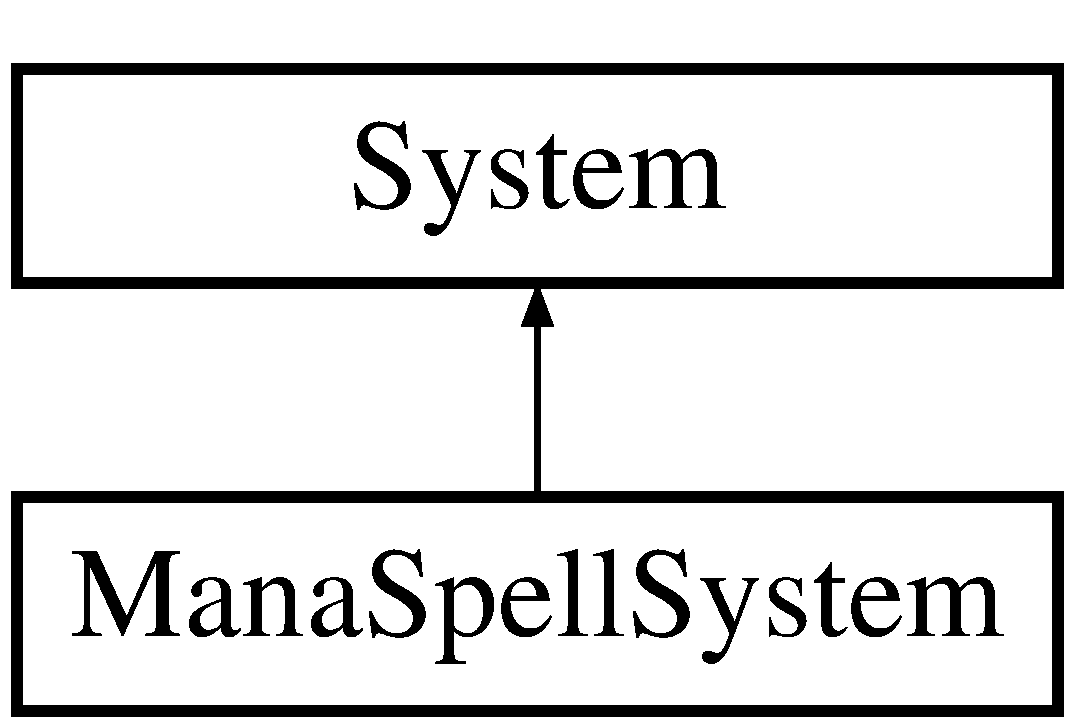
\includegraphics[height=2.000000cm]{class_mana_spell_system}
\end{center}
\end{figure}
\subsection*{Public Member Functions}
\begin{DoxyCompactItemize}
\item 
\hyperlink{class_mana_spell_system_a3ea9f85c878712cb8c41b0b26390f8f8}{Mana\+Spell\+System} (\hyperlink{class_entity_system}{Entity\+System} \&)
\begin{DoxyCompactList}\small\item\em Constructor. \end{DoxyCompactList}\item 
\hyperlink{class_mana_spell_system_acaca2ea30a3317e34cc6f8c28475a423}{$\sim$\+Mana\+Spell\+System} ()=default
\begin{DoxyCompactList}\small\item\em Destructor. \end{DoxyCompactList}\item 
void \hyperlink{class_mana_spell_system_a72ff0244c7ed729843fc82dde04b3477}{update} (tdt\+::real) override
\begin{DoxyCompactList}\small\item\em Regenerates mana if necessary and performs entity spell casting if off cooldown. \end{DoxyCompactList}\item 
void \hyperlink{class_mana_spell_system_a3fae933e8c9f595f03759654675b96e5}{set\+\_\+regen\+\_\+period} (tdt\+::real)
\begin{DoxyCompactList}\small\item\em Sets the time period between mana regens. \end{DoxyCompactList}\item 
tdt\+::real \hyperlink{class_mana_spell_system_a76f518959b92b7433d8af963d0a28fdd}{get\+\_\+regen\+\_\+period} () const 
\begin{DoxyCompactList}\small\item\em Returns the time period between mana regens. \end{DoxyCompactList}\end{DoxyCompactItemize}
\subsection*{Private Attributes}
\begin{DoxyCompactItemize}
\item 
\hyperlink{class_entity_system}{Entity\+System} \& \hyperlink{class_mana_spell_system_a907a818e62304a34d411c428e8989ee3}{entities\+\_\+}
\begin{DoxyCompactList}\small\item\em Entity system containing entities that this system works with. \end{DoxyCompactList}\item 
tdt\+::real \hyperlink{class_mana_spell_system_a01b27fb864d1dd85425acb87e7928129}{regen\+\_\+timer\+\_\+}
\begin{DoxyCompactList}\small\item\em Allow for dynamic periods between mana regeneration updates. \end{DoxyCompactList}\item 
tdt\+::real {\bfseries regen\+\_\+period\+\_\+}\hypertarget{class_mana_spell_system_aab19b08f7d2b73afd7e6b31dfbaa0020}{}\label{class_mana_spell_system_aab19b08f7d2b73afd7e6b31dfbaa0020}

\end{DoxyCompactItemize}


\subsection{Detailed Description}
Regenerates mana to the player and all entities that have mana. 

Also takes care of entity spell casting. 

Definition at line 11 of file Mana\+Spell\+System.\+hpp.



\subsection{Constructor \& Destructor Documentation}
\index{Mana\+Spell\+System@{Mana\+Spell\+System}!Mana\+Spell\+System@{Mana\+Spell\+System}}
\index{Mana\+Spell\+System@{Mana\+Spell\+System}!Mana\+Spell\+System@{Mana\+Spell\+System}}
\subsubsection[{\texorpdfstring{Mana\+Spell\+System(\+Entity\+System \&)}{ManaSpellSystem(EntitySystem &)}}]{\setlength{\rightskip}{0pt plus 5cm}Mana\+Spell\+System\+::\+Mana\+Spell\+System (
\begin{DoxyParamCaption}
\item[{{\bf Entity\+System} \&}]{ents}
\end{DoxyParamCaption}
)}\hypertarget{class_mana_spell_system_a3ea9f85c878712cb8c41b0b26390f8f8}{}\label{class_mana_spell_system_a3ea9f85c878712cb8c41b0b26390f8f8}


Constructor. 


\begin{DoxyParams}{Parameters}
{\em Entity} & system containing entities this system works with. \\
\hline
\end{DoxyParams}


Definition at line 6 of file Mana\+Spell\+System.\+cpp.

\index{Mana\+Spell\+System@{Mana\+Spell\+System}!````~Mana\+Spell\+System@{$\sim$\+Mana\+Spell\+System}}
\index{````~Mana\+Spell\+System@{$\sim$\+Mana\+Spell\+System}!Mana\+Spell\+System@{Mana\+Spell\+System}}
\subsubsection[{\texorpdfstring{$\sim$\+Mana\+Spell\+System()=default}{~ManaSpellSystem()=default}}]{\setlength{\rightskip}{0pt plus 5cm}Mana\+Spell\+System\+::$\sim$\+Mana\+Spell\+System (
\begin{DoxyParamCaption}
{}
\end{DoxyParamCaption}
)\hspace{0.3cm}{\ttfamily [default]}}\hypertarget{class_mana_spell_system_acaca2ea30a3317e34cc6f8c28475a423}{}\label{class_mana_spell_system_acaca2ea30a3317e34cc6f8c28475a423}


Destructor. 



\subsection{Member Function Documentation}
\index{Mana\+Spell\+System@{Mana\+Spell\+System}!get\+\_\+regen\+\_\+period@{get\+\_\+regen\+\_\+period}}
\index{get\+\_\+regen\+\_\+period@{get\+\_\+regen\+\_\+period}!Mana\+Spell\+System@{Mana\+Spell\+System}}
\subsubsection[{\texorpdfstring{get\+\_\+regen\+\_\+period() const }{get_regen_period() const }}]{\setlength{\rightskip}{0pt plus 5cm}tdt\+::real Mana\+Spell\+System\+::get\+\_\+regen\+\_\+period (
\begin{DoxyParamCaption}
{}
\end{DoxyParamCaption}
) const}\hypertarget{class_mana_spell_system_a76f518959b92b7433d8af963d0a28fdd}{}\label{class_mana_spell_system_a76f518959b92b7433d8af963d0a28fdd}


Returns the time period between mana regens. 



Definition at line 45 of file Mana\+Spell\+System.\+cpp.

\index{Mana\+Spell\+System@{Mana\+Spell\+System}!set\+\_\+regen\+\_\+period@{set\+\_\+regen\+\_\+period}}
\index{set\+\_\+regen\+\_\+period@{set\+\_\+regen\+\_\+period}!Mana\+Spell\+System@{Mana\+Spell\+System}}
\subsubsection[{\texorpdfstring{set\+\_\+regen\+\_\+period(tdt\+::real)}{set_regen_period(tdt::real)}}]{\setlength{\rightskip}{0pt plus 5cm}void Mana\+Spell\+System\+::set\+\_\+regen\+\_\+period (
\begin{DoxyParamCaption}
\item[{tdt\+::real}]{val}
\end{DoxyParamCaption}
)}\hypertarget{class_mana_spell_system_a3fae933e8c9f595f03759654675b96e5}{}\label{class_mana_spell_system_a3fae933e8c9f595f03759654675b96e5}


Sets the time period between mana regens. 


\begin{DoxyParams}{Parameters}
{\em The} & new time period. \\
\hline
\end{DoxyParams}


Definition at line 40 of file Mana\+Spell\+System.\+cpp.

\index{Mana\+Spell\+System@{Mana\+Spell\+System}!update@{update}}
\index{update@{update}!Mana\+Spell\+System@{Mana\+Spell\+System}}
\subsubsection[{\texorpdfstring{update(tdt\+::real) override}{update(tdt::real) override}}]{\setlength{\rightskip}{0pt plus 5cm}void Mana\+Spell\+System\+::update (
\begin{DoxyParamCaption}
\item[{tdt\+::real}]{delta}
\end{DoxyParamCaption}
)\hspace{0.3cm}{\ttfamily [override]}, {\ttfamily [virtual]}}\hypertarget{class_mana_spell_system_a72ff0244c7ed729843fc82dde04b3477}{}\label{class_mana_spell_system_a72ff0244c7ed729843fc82dde04b3477}


Regenerates mana if necessary and performs entity spell casting if off cooldown. 


\begin{DoxyParams}{Parameters}
{\em Time} & since last frame. \\
\hline
\end{DoxyParams}


Implements \hyperlink{class_system_a6d54c9bd38eb43d620a1451cb0925472}{System}.



Definition at line 10 of file Mana\+Spell\+System.\+cpp.



\subsection{Member Data Documentation}
\index{Mana\+Spell\+System@{Mana\+Spell\+System}!entities\+\_\+@{entities\+\_\+}}
\index{entities\+\_\+@{entities\+\_\+}!Mana\+Spell\+System@{Mana\+Spell\+System}}
\subsubsection[{\texorpdfstring{entities\+\_\+}{entities_}}]{\setlength{\rightskip}{0pt plus 5cm}{\bf Entity\+System}\& Mana\+Spell\+System\+::entities\+\_\+\hspace{0.3cm}{\ttfamily [private]}}\hypertarget{class_mana_spell_system_a907a818e62304a34d411c428e8989ee3}{}\label{class_mana_spell_system_a907a818e62304a34d411c428e8989ee3}


Entity system containing entities that this system works with. 



Definition at line 48 of file Mana\+Spell\+System.\+hpp.

\index{Mana\+Spell\+System@{Mana\+Spell\+System}!regen\+\_\+timer\+\_\+@{regen\+\_\+timer\+\_\+}}
\index{regen\+\_\+timer\+\_\+@{regen\+\_\+timer\+\_\+}!Mana\+Spell\+System@{Mana\+Spell\+System}}
\subsubsection[{\texorpdfstring{regen\+\_\+timer\+\_\+}{regen_timer_}}]{\setlength{\rightskip}{0pt plus 5cm}tdt\+::real Mana\+Spell\+System\+::regen\+\_\+timer\+\_\+\hspace{0.3cm}{\ttfamily [private]}}\hypertarget{class_mana_spell_system_a01b27fb864d1dd85425acb87e7928129}{}\label{class_mana_spell_system_a01b27fb864d1dd85425acb87e7928129}


Allow for dynamic periods between mana regeneration updates. 



Definition at line 54 of file Mana\+Spell\+System.\+hpp.



The documentation for this class was generated from the following files\+:\begin{DoxyCompactItemize}
\item 
systems/Mana\+Spell\+System.\+hpp\item 
systems/Mana\+Spell\+System.\+cpp\end{DoxyCompactItemize}

\hypertarget{structutil_1_1heuristic_1_1_m_a_n_h_a_t_t_a_n___d_i_s_t_a_n_c_e}{}\section{util\+:\+:heuristic\+:\+:M\+A\+N\+H\+A\+T\+T\+A\+N\+\_\+\+D\+I\+S\+T\+A\+N\+CE Struct Reference}
\label{structutil_1_1heuristic_1_1_m_a_n_h_a_t_t_a_n___d_i_s_t_a_n_c_e}\index{util\+::heuristic\+::\+M\+A\+N\+H\+A\+T\+T\+A\+N\+\_\+\+D\+I\+S\+T\+A\+N\+CE@{util\+::heuristic\+::\+M\+A\+N\+H\+A\+T\+T\+A\+N\+\_\+\+D\+I\+S\+T\+A\+N\+CE}}


Returns the manhattan distance between two nodes.  




{\ttfamily \#include $<$Pathfinding\+Algorithms.\+hpp$>$}

Inheritance diagram for util\+:\+:heuristic\+:\+:M\+A\+N\+H\+A\+T\+T\+A\+N\+\_\+\+D\+I\+S\+T\+A\+N\+CE\+:\begin{figure}[H]
\begin{center}
\leavevmode
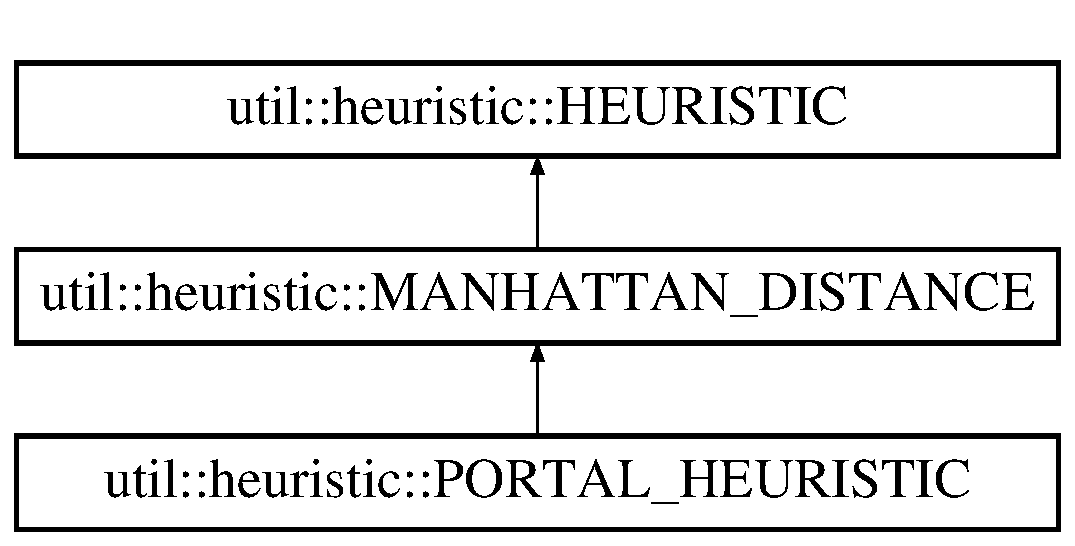
\includegraphics[height=3.000000cm]{structutil_1_1heuristic_1_1_m_a_n_h_a_t_t_a_n___d_i_s_t_a_n_c_e}
\end{center}
\end{figure}
\subsection*{Public Member Functions}
\begin{DoxyCompactItemize}
\item 
{\bfseries M\+A\+N\+H\+A\+T\+T\+A\+N\+\_\+\+D\+I\+S\+T\+A\+N\+CE} (\hyperlink{class_entity_system}{Entity\+System} \&ents)\hypertarget{structutil_1_1heuristic_1_1_m_a_n_h_a_t_t_a_n___d_i_s_t_a_n_c_e_ad14e300361283f50d728e5a2c6005fb5}{}\label{structutil_1_1heuristic_1_1_m_a_n_h_a_t_t_a_n___d_i_s_t_a_n_c_e_ad14e300361283f50d728e5a2c6005fb5}

\item 
tdt\+::real {\bfseries get\+\_\+cost} (tdt\+::uint id1, tdt\+::uint id2) override\hypertarget{structutil_1_1heuristic_1_1_m_a_n_h_a_t_t_a_n___d_i_s_t_a_n_c_e_a9ef25541d53eb8b7ab5f8fcdd08b384a}{}\label{structutil_1_1heuristic_1_1_m_a_n_h_a_t_t_a_n___d_i_s_t_a_n_c_e_a9ef25541d53eb8b7ab5f8fcdd08b384a}

\end{DoxyCompactItemize}
\subsection*{Additional Inherited Members}


\subsection{Detailed Description}
Returns the manhattan distance between two nodes. 

(Well, actually, it\textquotesingle{}s an octal distance \+:) 

Definition at line 206 of file Pathfinding\+Algorithms.\+hpp.



The documentation for this struct was generated from the following file\+:\begin{DoxyCompactItemize}
\item 
tools/Pathfinding\+Algorithms.\+hpp\end{DoxyCompactItemize}

\hypertarget{class_message_to_player_window}{}\section{Message\+To\+Player\+Window Class Reference}
\label{class_message_to_player_window}\index{Message\+To\+Player\+Window@{Message\+To\+Player\+Window}}


A window that can show the player a text message with 1, 2 or 3 buttons (custom labels) that can call assigned functions.  




{\ttfamily \#include $<$Message\+To\+Player\+Window.\+hpp$>$}

Inheritance diagram for Message\+To\+Player\+Window\+:\begin{figure}[H]
\begin{center}
\leavevmode
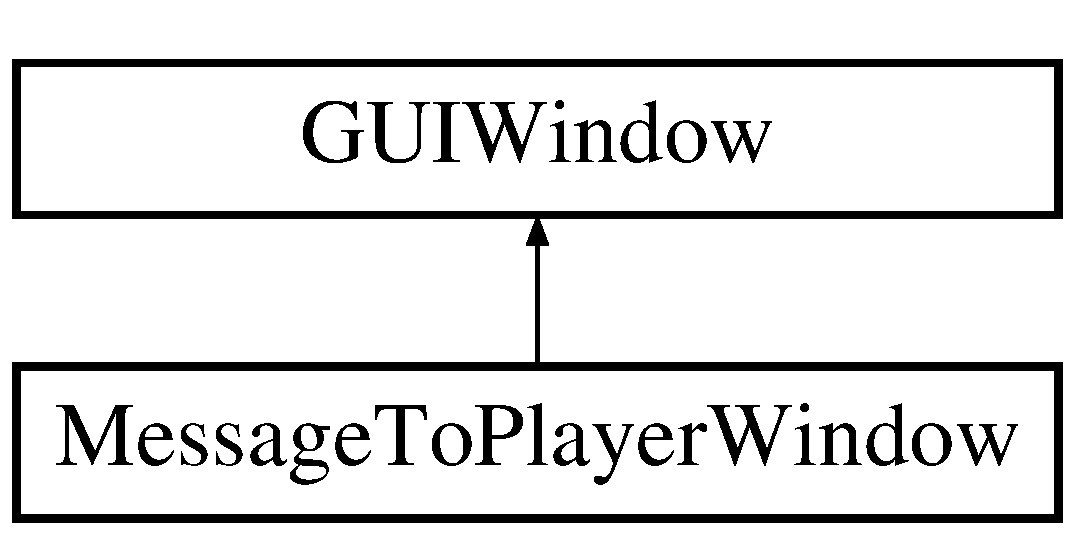
\includegraphics[height=2.000000cm]{class_message_to_player_window}
\end{center}
\end{figure}
\subsection*{Public Member Functions}
\begin{DoxyCompactItemize}
\item 
\hyperlink{class_message_to_player_window_a1522c842309df689cf032d9b3de76fa7}{Message\+To\+Player\+Window} ()
\begin{DoxyCompactList}\small\item\em Constructor. \end{DoxyCompactList}\item 
\hyperlink{class_message_to_player_window_a09180c464e2bdafec3657d4dd3692d99}{$\sim$\+Message\+To\+Player\+Window} ()=default
\begin{DoxyCompactList}\small\item\em Destructor. \end{DoxyCompactList}\item 
void \hyperlink{class_message_to_player_window_aa61b87c640a95dbaafe796392522b0b9}{show} (const std\+::string \&=\char`\"{}N\+O\+NE\char`\"{}, const std\+::string \&=\char`\"{}N\+O\+NE\char`\"{}, const std\+::string \&=\char`\"{}N\+O\+NE\char`\"{}, const std\+::string \&=\char`\"{}N\+O\+NE\char`\"{})
\begin{DoxyCompactList}\small\item\em Shows a given text message to the player and assigns callbacks to the buttons. \end{DoxyCompactList}\item 
void \hyperlink{class_message_to_player_window_aaa52044d01c842b03df4e83b58be4098}{set\+\_\+butt\+\_\+label} (const std\+::string \&, const std\+::string \&)
\begin{DoxyCompactList}\small\item\em Sets the label of a given button. \end{DoxyCompactList}\item 
void \hyperlink{class_message_to_player_window_af0c2aad5fd5b2d502641a1249dcfe650}{reset\+\_\+butt\+\_\+labels} ()
\begin{DoxyCompactList}\small\item\em Resets the button labels to their default values. \end{DoxyCompactList}\end{DoxyCompactItemize}
\subsection*{Protected Member Functions}
\begin{DoxyCompactItemize}
\item 
void \hyperlink{class_message_to_player_window_a5eb87ad777baa5c23a3cdb262512d9e3}{init\+\_\+} ()
\begin{DoxyCompactList}\small\item\em Initializes this window. \end{DoxyCompactList}\end{DoxyCompactItemize}
\subsection*{Private Attributes}
\begin{DoxyCompactItemize}
\item 
\hyperlink{classlpp_1_1_script}{lpp\+::\+Script} \& \hyperlink{class_message_to_player_window_af02854c06fe25800f3dc44e23848a9df}{script\+\_\+}
\begin{DoxyCompactList}\small\item\em Reference to the scripting engine for easier use when calling Lua callbacks. \end{DoxyCompactList}\item 
std\+::string \hyperlink{class_message_to_player_window_a9ee321677a2a774e2e147ddbaef35ef5}{ok\+\_\+func\+\_\+}
\begin{DoxyCompactList}\small\item\em Labels of the buttons. \end{DoxyCompactList}\item 
std\+::string {\bfseries yes\+\_\+func\+\_\+}\hypertarget{class_message_to_player_window_a97cc7136d9ea8fd6e8397871555a6e0b}{}\label{class_message_to_player_window_a97cc7136d9ea8fd6e8397871555a6e0b}

\item 
std\+::string {\bfseries no\+\_\+func\+\_\+}\hypertarget{class_message_to_player_window_ae17d66e7dd9ae682ce23f89e79906e6b}{}\label{class_message_to_player_window_ae17d66e7dd9ae682ce23f89e79906e6b}

\end{DoxyCompactItemize}
\subsection*{Additional Inherited Members}


\subsection{Detailed Description}
A window that can show the player a text message with 1, 2 or 3 buttons (custom labels) that can call assigned functions. 

Button names\+: (used for setting labels) 1st on the left\+: NO 2nd on the left\+: Y\+ES 1st on the right\+: OK 

Definition at line 18 of file Message\+To\+Player\+Window.\+hpp.



\subsection{Constructor \& Destructor Documentation}
\index{Message\+To\+Player\+Window@{Message\+To\+Player\+Window}!Message\+To\+Player\+Window@{Message\+To\+Player\+Window}}
\index{Message\+To\+Player\+Window@{Message\+To\+Player\+Window}!Message\+To\+Player\+Window@{Message\+To\+Player\+Window}}
\subsubsection[{\texorpdfstring{Message\+To\+Player\+Window()}{MessageToPlayerWindow()}}]{\setlength{\rightskip}{0pt plus 5cm}Message\+To\+Player\+Window\+::\+Message\+To\+Player\+Window (
\begin{DoxyParamCaption}
{}
\end{DoxyParamCaption}
)}\hypertarget{class_message_to_player_window_a1522c842309df689cf032d9b3de76fa7}{}\label{class_message_to_player_window_a1522c842309df689cf032d9b3de76fa7}


Constructor. 



Definition at line 5 of file Message\+To\+Player\+Window.\+cpp.

\index{Message\+To\+Player\+Window@{Message\+To\+Player\+Window}!````~Message\+To\+Player\+Window@{$\sim$\+Message\+To\+Player\+Window}}
\index{````~Message\+To\+Player\+Window@{$\sim$\+Message\+To\+Player\+Window}!Message\+To\+Player\+Window@{Message\+To\+Player\+Window}}
\subsubsection[{\texorpdfstring{$\sim$\+Message\+To\+Player\+Window()=default}{~MessageToPlayerWindow()=default}}]{\setlength{\rightskip}{0pt plus 5cm}Message\+To\+Player\+Window\+::$\sim$\+Message\+To\+Player\+Window (
\begin{DoxyParamCaption}
{}
\end{DoxyParamCaption}
)\hspace{0.3cm}{\ttfamily [default]}}\hypertarget{class_message_to_player_window_a09180c464e2bdafec3657d4dd3692d99}{}\label{class_message_to_player_window_a09180c464e2bdafec3657d4dd3692d99}


Destructor. 



\subsection{Member Function Documentation}
\index{Message\+To\+Player\+Window@{Message\+To\+Player\+Window}!init\+\_\+@{init\+\_\+}}
\index{init\+\_\+@{init\+\_\+}!Message\+To\+Player\+Window@{Message\+To\+Player\+Window}}
\subsubsection[{\texorpdfstring{init\+\_\+()}{init_()}}]{\setlength{\rightskip}{0pt plus 5cm}void Message\+To\+Player\+Window\+::init\+\_\+ (
\begin{DoxyParamCaption}
{}
\end{DoxyParamCaption}
)\hspace{0.3cm}{\ttfamily [protected]}, {\ttfamily [virtual]}}\hypertarget{class_message_to_player_window_a5eb87ad777baa5c23a3cdb262512d9e3}{}\label{class_message_to_player_window_a5eb87ad777baa5c23a3cdb262512d9e3}


Initializes this window. 



Implements \hyperlink{class_g_u_i_window_a2a7c011363f401a57a26cc7c7652bdfd}{G\+U\+I\+Window}.



Definition at line 53 of file Message\+To\+Player\+Window.\+cpp.

\index{Message\+To\+Player\+Window@{Message\+To\+Player\+Window}!reset\+\_\+butt\+\_\+labels@{reset\+\_\+butt\+\_\+labels}}
\index{reset\+\_\+butt\+\_\+labels@{reset\+\_\+butt\+\_\+labels}!Message\+To\+Player\+Window@{Message\+To\+Player\+Window}}
\subsubsection[{\texorpdfstring{reset\+\_\+butt\+\_\+labels()}{reset_butt_labels()}}]{\setlength{\rightskip}{0pt plus 5cm}void Message\+To\+Player\+Window\+::reset\+\_\+butt\+\_\+labels (
\begin{DoxyParamCaption}
{}
\end{DoxyParamCaption}
)}\hypertarget{class_message_to_player_window_af0c2aad5fd5b2d502641a1249dcfe650}{}\label{class_message_to_player_window_af0c2aad5fd5b2d502641a1249dcfe650}


Resets the button labels to their default values. 

(\char`\"{}\+O\+K\char`\"{}, \char`\"{}\+Y\+E\+S\char`\"{} and \char`\"{}\+N\+O\char`\"{}) 

Definition at line 46 of file Message\+To\+Player\+Window.\+cpp.

\index{Message\+To\+Player\+Window@{Message\+To\+Player\+Window}!set\+\_\+butt\+\_\+label@{set\+\_\+butt\+\_\+label}}
\index{set\+\_\+butt\+\_\+label@{set\+\_\+butt\+\_\+label}!Message\+To\+Player\+Window@{Message\+To\+Player\+Window}}
\subsubsection[{\texorpdfstring{set\+\_\+butt\+\_\+label(const std\+::string \&, const std\+::string \&)}{set_butt_label(const std::string &, const std::string &)}}]{\setlength{\rightskip}{0pt plus 5cm}void Message\+To\+Player\+Window\+::set\+\_\+butt\+\_\+label (
\begin{DoxyParamCaption}
\item[{const std\+::string \&}]{butt, }
\item[{const std\+::string \&}]{val}
\end{DoxyParamCaption}
)}\hypertarget{class_message_to_player_window_aaa52044d01c842b03df4e83b58be4098}{}\label{class_message_to_player_window_aaa52044d01c842b03df4e83b58be4098}


Sets the label of a given button. 


\begin{DoxyParams}{Parameters}
{\em The} & name of the button (OK, Y\+ES, NO). \\
\hline
{\em The} & new label. \\
\hline
\end{DoxyParams}


Definition at line 41 of file Message\+To\+Player\+Window.\+cpp.

\index{Message\+To\+Player\+Window@{Message\+To\+Player\+Window}!show@{show}}
\index{show@{show}!Message\+To\+Player\+Window@{Message\+To\+Player\+Window}}
\subsubsection[{\texorpdfstring{show(const std\+::string \&=""N\+O\+NE"", const std\+::string \&=""N\+O\+NE"", const std\+::string \&=""N\+O\+NE"", const std\+::string \&=""N\+O\+NE"")}{show(const std::string &="NONE", const std::string &="NONE", const std::string &="NONE", const std::string &="NONE")}}]{\setlength{\rightskip}{0pt plus 5cm}void Message\+To\+Player\+Window\+::show (
\begin{DoxyParamCaption}
\item[{const std\+::string \&}]{msg = {\ttfamily \char`\"{}NONE\char`\"{}}, }
\item[{const std\+::string \&}]{ok = {\ttfamily \char`\"{}NONE\char`\"{}}, }
\item[{const std\+::string \&}]{yes = {\ttfamily \char`\"{}NONE\char`\"{}}, }
\item[{const std\+::string \&}]{no = {\ttfamily \char`\"{}NONE\char`\"{}}}
\end{DoxyParamCaption}
)}\hypertarget{class_message_to_player_window_aa61b87c640a95dbaafe796392522b0b9}{}\label{class_message_to_player_window_aa61b87c640a95dbaafe796392522b0b9}


Shows a given text message to the player and assigns callbacks to the buttons. 


\begin{DoxyParams}{Parameters}
{\em The} & message. \\
\hline
{\em Callback} & for the OK button. \\
\hline
{\em Callback} & for the Y\+ES button. \\
\hline
{\em Callback} & for the NO button. \\
\hline
\end{DoxyParams}
\begin{DoxyNote}{Note}
If a callback passes is \char`\"{}\+N\+O\+N\+E\char`\"{}, the assigned button will not be shown. 

The callbacks are strings of names of the Lua functions that ought to be called when the button is pressed. 
\end{DoxyNote}


Definition at line 10 of file Message\+To\+Player\+Window.\+cpp.



\subsection{Member Data Documentation}
\index{Message\+To\+Player\+Window@{Message\+To\+Player\+Window}!ok\+\_\+func\+\_\+@{ok\+\_\+func\+\_\+}}
\index{ok\+\_\+func\+\_\+@{ok\+\_\+func\+\_\+}!Message\+To\+Player\+Window@{Message\+To\+Player\+Window}}
\subsubsection[{\texorpdfstring{ok\+\_\+func\+\_\+}{ok_func_}}]{\setlength{\rightskip}{0pt plus 5cm}std\+::string Message\+To\+Player\+Window\+::ok\+\_\+func\+\_\+\hspace{0.3cm}{\ttfamily [private]}}\hypertarget{class_message_to_player_window_a9ee321677a2a774e2e147ddbaef35ef5}{}\label{class_message_to_player_window_a9ee321677a2a774e2e147ddbaef35ef5}


Labels of the buttons. 



Definition at line 74 of file Message\+To\+Player\+Window.\+hpp.

\index{Message\+To\+Player\+Window@{Message\+To\+Player\+Window}!script\+\_\+@{script\+\_\+}}
\index{script\+\_\+@{script\+\_\+}!Message\+To\+Player\+Window@{Message\+To\+Player\+Window}}
\subsubsection[{\texorpdfstring{script\+\_\+}{script_}}]{\setlength{\rightskip}{0pt plus 5cm}{\bf lpp\+::\+Script}\& Message\+To\+Player\+Window\+::script\+\_\+\hspace{0.3cm}{\ttfamily [private]}}\hypertarget{class_message_to_player_window_af02854c06fe25800f3dc44e23848a9df}{}\label{class_message_to_player_window_af02854c06fe25800f3dc44e23848a9df}


Reference to the scripting engine for easier use when calling Lua callbacks. 



Definition at line 69 of file Message\+To\+Player\+Window.\+hpp.



The documentation for this class was generated from the following files\+:\begin{DoxyCompactItemize}
\item 
gui/Message\+To\+Player\+Window.\+hpp\item 
gui/Message\+To\+Player\+Window.\+cpp\end{DoxyCompactItemize}

\hypertarget{struct_mine_component}{}\section{Mine\+Component Struct Reference}
\label{struct_mine_component}\index{Mine\+Component@{Mine\+Component}}


Dummy component that signals that an entity having it can be mined.  




{\ttfamily \#include $<$Components.\+hpp$>$}

\subsection*{Static Public Attributes}
\begin{DoxyCompactItemize}
\item 
static constexpr int {\bfseries type} = 25\hypertarget{struct_mine_component_a875d1a13fd67728798e8544597176c25}{}\label{struct_mine_component_a875d1a13fd67728798e8544597176c25}

\end{DoxyCompactItemize}


\subsection{Detailed Description}
Dummy component that signals that an entity having it can be mined. 

Definition at line 617 of file Components.\+hpp.



The documentation for this struct was generated from the following file\+:\begin{DoxyCompactItemize}
\item 
Components.\+hpp\end{DoxyCompactItemize}

\hypertarget{struct_movement_component}{}\section{Movement\+Component Struct Reference}
\label{struct_movement_component}\index{Movement\+Component@{Movement\+Component}}


Holds info related to movement, if an entity has this component it should also have a Physics component (containing the entity\textquotesingle{}s position), otherwise the \hyperlink{class_movement_system}{Movement\+System} might not work correctly.  




{\ttfamily \#include $<$Components.\+hpp$>$}

\subsection*{Public Member Functions}
\begin{DoxyCompactItemize}
\item 
{\bfseries Movement\+Component} (tdt\+::real speed=0.f)\hypertarget{struct_movement_component_add6cc4d335eacf819fc740fee0481dad}{}\label{struct_movement_component_add6cc4d335eacf819fc740fee0481dad}

\item 
{\bfseries Movement\+Component} (const \hyperlink{struct_movement_component}{Movement\+Component} \&)=default\hypertarget{struct_movement_component_a4d00d816a717fab21e939bf939b420d3}{}\label{struct_movement_component_a4d00d816a717fab21e939bf939b420d3}

\item 
{\bfseries Movement\+Component} (\hyperlink{struct_movement_component}{Movement\+Component} \&\&)=default\hypertarget{struct_movement_component_a27b68675aafa43ae2aed17a72618bd05}{}\label{struct_movement_component_a27b68675aafa43ae2aed17a72618bd05}

\item 
\hyperlink{struct_movement_component}{Movement\+Component} \& {\bfseries operator=} (const \hyperlink{struct_movement_component}{Movement\+Component} \&)=default\hypertarget{struct_movement_component_ab7d1f86d8048f4927affec173751d932}{}\label{struct_movement_component_ab7d1f86d8048f4927affec173751d932}

\item 
\hyperlink{struct_movement_component}{Movement\+Component} \& {\bfseries operator=} (\hyperlink{struct_movement_component}{Movement\+Component} \&\&)=default\hypertarget{struct_movement_component_aa5fec9c8dbd615bc3771eaf696e6a914}{}\label{struct_movement_component_aa5fec9c8dbd615bc3771eaf696e6a914}

\end{DoxyCompactItemize}
\subsection*{Public Attributes}
\begin{DoxyCompactItemize}
\item 
tdt\+::real {\bfseries speed\+\_\+modifier}\hypertarget{struct_movement_component_afcb4440b43821b991b8f09825d00bc46}{}\label{struct_movement_component_afcb4440b43821b991b8f09825d00bc46}

\item 
tdt\+::real {\bfseries original\+\_\+speed}\hypertarget{struct_movement_component_aee69070da125d18a4d6439079ed398f9}{}\label{struct_movement_component_aee69070da125d18a4d6439079ed398f9}

\end{DoxyCompactItemize}
\subsection*{Static Public Attributes}
\begin{DoxyCompactItemize}
\item 
static constexpr int {\bfseries type} = 4\hypertarget{struct_movement_component_a5e597e875ec732aebb8005074236feec}{}\label{struct_movement_component_a5e597e875ec732aebb8005074236feec}

\end{DoxyCompactItemize}


\subsection{Detailed Description}
Holds info related to movement, if an entity has this component it should also have a Physics component (containing the entity\textquotesingle{}s position), otherwise the \hyperlink{class_movement_system}{Movement\+System} might not work correctly. 

Definition at line 132 of file Components.\+hpp.



The documentation for this struct was generated from the following file\+:\begin{DoxyCompactItemize}
\item 
Components.\+hpp\end{DoxyCompactItemize}

\hypertarget{class_movement_system}{}\section{Movement\+System Class Reference}
\label{class_movement_system}\index{Movement\+System@{Movement\+System}}


\hyperlink{class_system}{System} handling movement related updates and containing movement \& physics related methods.  




{\ttfamily \#include $<$Movement\+System.\+hpp$>$}

Inheritance diagram for Movement\+System\+:\begin{figure}[H]
\begin{center}
\leavevmode
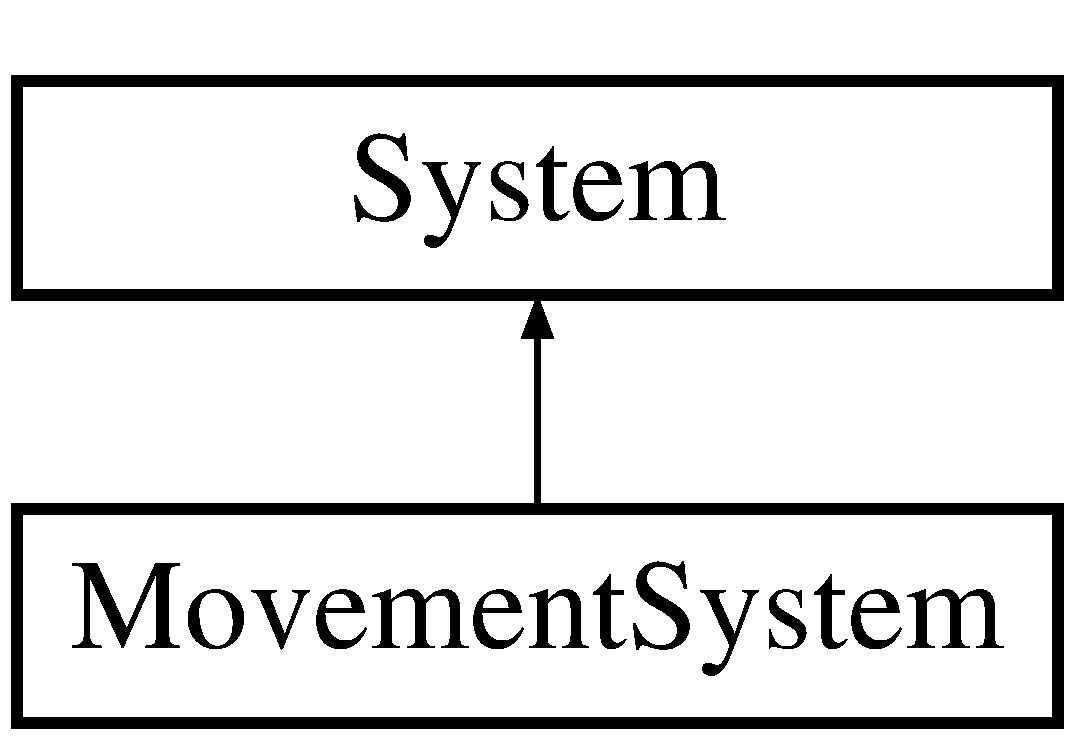
\includegraphics[height=2.000000cm]{class_movement_system}
\end{center}
\end{figure}
\subsection*{Public Member Functions}
\begin{DoxyCompactItemize}
\item 
\hyperlink{class_movement_system_ac79c2f7549bf24bb08b020e4bd0928a0}{Movement\+System} (\hyperlink{class_entity_system}{Entity\+System} \&)
\begin{DoxyCompactList}\small\item\em Constructor. \end{DoxyCompactList}\item 
\hyperlink{class_movement_system_a7389ab211f0da0cf859570d23ffb70fa}{$\sim$\+Movement\+System} ()
\begin{DoxyCompactList}\small\item\em Destructor. \end{DoxyCompactList}\item 
void \hyperlink{class_movement_system_a005915a7fff5eaf8f1e644e07ccda9e4}{update} (Ogre\+::\+Real)
\begin{DoxyCompactList}\small\item\em Updates the movement system. \end{DoxyCompactList}\item 
bool \hyperlink{class_movement_system_ae986dc2fb886b40fac2ab97a1c21d934}{can\+\_\+move\+\_\+to} (std\+::size\+\_\+t, Ogre\+::\+Vector3)
\begin{DoxyCompactList}\small\item\em Returns true if a given entity can move to a given point in space, false otherwise. \end{DoxyCompactList}\item 
bool \hyperlink{class_movement_system_a223e95da80379c936d01790ca449a0de}{checked\+\_\+move} (std\+::size\+\_\+t, Ogre\+::\+Vector3)
\begin{DoxyCompactList}\small\item\em Sets a given entity to move in a given direction, returns true if such movement is possible and false otherwise. \end{DoxyCompactList}\item 
bool \hyperlink{class_movement_system_a7cd808c936ad925fc5b15d76e9d52afd}{move} (std\+::size\+\_\+t, Ogre\+::\+Vector3)
\begin{DoxyCompactList}\small\item\em Sets a given entity to move in a given direction, returns true if such movement is possible and false otherwise. \end{DoxyCompactList}\end{DoxyCompactItemize}
\subsection*{Private Attributes}
\begin{DoxyCompactItemize}
\item 
\hyperlink{class_entity_system}{Entity\+System} \& \hyperlink{class_movement_system_a373d446bb2c853079f63437629d6044b}{entities\+\_\+}
\begin{DoxyCompactList}\small\item\em Reference to the game\textquotesingle{}s entity system. \end{DoxyCompactList}\item 
Ogre\+::\+Real \hyperlink{class_movement_system_aca59e8025a42f269c245d0ecbcab396c}{last\+\_\+delta\+\_\+}
\begin{DoxyCompactList}\small\item\em Time between the last frame and this frame, used so that lua calls to the move functions still use the time of this frame. \end{DoxyCompactList}\end{DoxyCompactItemize}


\subsection{Detailed Description}
\hyperlink{class_system}{System} handling movement related updates and containing movement \& physics related methods. 

Definition at line 10 of file Movement\+System.\+hpp.



\subsection{Constructor \& Destructor Documentation}
\index{Movement\+System@{Movement\+System}!Movement\+System@{Movement\+System}}
\index{Movement\+System@{Movement\+System}!Movement\+System@{Movement\+System}}
\subsubsection[{\texorpdfstring{Movement\+System(\+Entity\+System \&)}{MovementSystem(EntitySystem &)}}]{\setlength{\rightskip}{0pt plus 5cm}Movement\+System\+::\+Movement\+System (
\begin{DoxyParamCaption}
\item[{{\bf Entity\+System} \&}]{ents}
\end{DoxyParamCaption}
)}\hypertarget{class_movement_system_ac79c2f7549bf24bb08b020e4bd0928a0}{}\label{class_movement_system_ac79c2f7549bf24bb08b020e4bd0928a0}


Constructor. 


\begin{DoxyParams}{Parameters}
{\em Reference} & to the game\textquotesingle{}s entity system. \\
\hline
\end{DoxyParams}


Definition at line 7 of file Movement\+System.\+cpp.

\index{Movement\+System@{Movement\+System}!````~Movement\+System@{$\sim$\+Movement\+System}}
\index{````~Movement\+System@{$\sim$\+Movement\+System}!Movement\+System@{Movement\+System}}
\subsubsection[{\texorpdfstring{$\sim$\+Movement\+System()}{~MovementSystem()}}]{\setlength{\rightskip}{0pt plus 5cm}Movement\+System\+::$\sim$\+Movement\+System (
\begin{DoxyParamCaption}
{}
\end{DoxyParamCaption}
)\hspace{0.3cm}{\ttfamily [inline]}}\hypertarget{class_movement_system_a7389ab211f0da0cf859570d23ffb70fa}{}\label{class_movement_system_a7389ab211f0da0cf859570d23ffb70fa}


Destructor. 



Definition at line 22 of file Movement\+System.\+hpp.



\subsection{Member Function Documentation}
\index{Movement\+System@{Movement\+System}!can\+\_\+move\+\_\+to@{can\+\_\+move\+\_\+to}}
\index{can\+\_\+move\+\_\+to@{can\+\_\+move\+\_\+to}!Movement\+System@{Movement\+System}}
\subsubsection[{\texorpdfstring{can\+\_\+move\+\_\+to(std\+::size\+\_\+t, Ogre\+::\+Vector3)}{can_move_to(std::size_t, Ogre::Vector3)}}]{\setlength{\rightskip}{0pt plus 5cm}bool Movement\+System\+::can\+\_\+move\+\_\+to (
\begin{DoxyParamCaption}
\item[{std\+::size\+\_\+t}]{id, }
\item[{Ogre\+::\+Vector3}]{pos}
\end{DoxyParamCaption}
)}\hypertarget{class_movement_system_ae986dc2fb886b40fac2ab97a1c21d934}{}\label{class_movement_system_ae986dc2fb886b40fac2ab97a1c21d934}


Returns true if a given entity can move to a given point in space, false otherwise. 


\begin{DoxyParams}{Parameters}
{\em ID} & of the entity. \\
\hline
{\em Target} & coordinate. \\
\hline
\end{DoxyParams}


Definition at line 49 of file Movement\+System.\+cpp.

\index{Movement\+System@{Movement\+System}!checked\+\_\+move@{checked\+\_\+move}}
\index{checked\+\_\+move@{checked\+\_\+move}!Movement\+System@{Movement\+System}}
\subsubsection[{\texorpdfstring{checked\+\_\+move(std\+::size\+\_\+t, Ogre\+::\+Vector3)}{checked_move(std::size_t, Ogre::Vector3)}}]{\setlength{\rightskip}{0pt plus 5cm}bool Movement\+System\+::checked\+\_\+move (
\begin{DoxyParamCaption}
\item[{std\+::size\+\_\+t}]{id, }
\item[{Ogre\+::\+Vector3}]{dir\+\_\+vector}
\end{DoxyParamCaption}
)}\hypertarget{class_movement_system_a223e95da80379c936d01790ca449a0de}{}\label{class_movement_system_a223e95da80379c936d01790ca449a0de}


Sets a given entity to move in a given direction, returns true if such movement is possible and false otherwise. 

The move will then be applied in the update method. 
\begin{DoxyParams}{Parameters}
{\em ID} & of the entity. \\
\hline
{\em Directional} & vector. \\
\hline
\end{DoxyParams}
\begin{DoxyNote}{Note}
Every vector passed to this method should be normalised and the length of the move will be increased by the entity\textquotesingle{}s speed modifier. This is not enforced though. 

Checks for collisions. 
\end{DoxyNote}


Definition at line 85 of file Movement\+System.\+cpp.

\index{Movement\+System@{Movement\+System}!move@{move}}
\index{move@{move}!Movement\+System@{Movement\+System}}
\subsubsection[{\texorpdfstring{move(std\+::size\+\_\+t, Ogre\+::\+Vector3)}{move(std::size_t, Ogre::Vector3)}}]{\setlength{\rightskip}{0pt plus 5cm}bool Movement\+System\+::move (
\begin{DoxyParamCaption}
\item[{std\+::size\+\_\+t}]{id, }
\item[{Ogre\+::\+Vector3}]{dir\+\_\+vector}
\end{DoxyParamCaption}
)}\hypertarget{class_movement_system_a7cd808c936ad925fc5b15d76e9d52afd}{}\label{class_movement_system_a7cd808c936ad925fc5b15d76e9d52afd}


Sets a given entity to move in a given direction, returns true if such movement is possible and false otherwise. 

The move will then be applied in the update method. 
\begin{DoxyParams}{Parameters}
{\em ID} & of the entity. \\
\hline
{\em Directional} & vector. \\
\hline
\end{DoxyParams}
\begin{DoxyNote}{Note}
Every vector passed to this method should be normalised and the length of the move will be increased by the entity\textquotesingle{}s speed modifier. This is not enforced though. 

Does not check for collisions. 
\end{DoxyNote}


Definition at line 110 of file Movement\+System.\+cpp.

\index{Movement\+System@{Movement\+System}!update@{update}}
\index{update@{update}!Movement\+System@{Movement\+System}}
\subsubsection[{\texorpdfstring{update(\+Ogre\+::\+Real)}{update(Ogre::Real)}}]{\setlength{\rightskip}{0pt plus 5cm}void Movement\+System\+::update (
\begin{DoxyParamCaption}
\item[{Ogre\+::\+Real}]{delta}
\end{DoxyParamCaption}
)\hspace{0.3cm}{\ttfamily [virtual]}}\hypertarget{class_movement_system_a005915a7fff5eaf8f1e644e07ccda9e4}{}\label{class_movement_system_a005915a7fff5eaf8f1e644e07ccda9e4}


Updates the movement system. 


\begin{DoxyParams}{Parameters}
{\em Time} & since the last frame. \\
\hline
\end{DoxyParams}


Implements \hyperlink{class_system_a6d54c9bd38eb43d620a1451cb0925472}{System}.



Definition at line 11 of file Movement\+System.\+cpp.



\subsection{Member Data Documentation}
\index{Movement\+System@{Movement\+System}!entities\+\_\+@{entities\+\_\+}}
\index{entities\+\_\+@{entities\+\_\+}!Movement\+System@{Movement\+System}}
\subsubsection[{\texorpdfstring{entities\+\_\+}{entities_}}]{\setlength{\rightskip}{0pt plus 5cm}{\bf Entity\+System}\& Movement\+System\+::entities\+\_\+\hspace{0.3cm}{\ttfamily [private]}}\hypertarget{class_movement_system_a373d446bb2c853079f63437629d6044b}{}\label{class_movement_system_a373d446bb2c853079f63437629d6044b}


Reference to the game\textquotesingle{}s entity system. 



Definition at line 63 of file Movement\+System.\+hpp.

\index{Movement\+System@{Movement\+System}!last\+\_\+delta\+\_\+@{last\+\_\+delta\+\_\+}}
\index{last\+\_\+delta\+\_\+@{last\+\_\+delta\+\_\+}!Movement\+System@{Movement\+System}}
\subsubsection[{\texorpdfstring{last\+\_\+delta\+\_\+}{last_delta_}}]{\setlength{\rightskip}{0pt plus 5cm}Ogre\+::\+Real Movement\+System\+::last\+\_\+delta\+\_\+\hspace{0.3cm}{\ttfamily [private]}}\hypertarget{class_movement_system_aca59e8025a42f269c245d0ecbcab396c}{}\label{class_movement_system_aca59e8025a42f269c245d0ecbcab396c}


Time between the last frame and this frame, used so that lua calls to the move functions still use the time of this frame. 



Definition at line 69 of file Movement\+System.\+hpp.



The documentation for this class was generated from the following files\+:\begin{DoxyCompactItemize}
\item 
systems/Movement\+System.\+hpp\item 
systems/Movement\+System.\+cpp\end{DoxyCompactItemize}

\hypertarget{struct_name_component}{}\section{Name\+Component Struct Reference}
\label{struct_name_component}\index{Name\+Component@{Name\+Component}}


Name of the entity shown in the entity viewer.  




{\ttfamily \#include $<$Components.\+hpp$>$}

\subsection*{Public Member Functions}
\begin{DoxyCompactItemize}
\item 
{\bfseries Name\+Component} (std\+::string \&\&n=\char`\"{}E\+R\+R\+OR\char`\"{})\hypertarget{struct_name_component_aa9663d779d531d990cca4d7af5ef0d21}{}\label{struct_name_component_aa9663d779d531d990cca4d7af5ef0d21}

\item 
{\bfseries Name\+Component} (const \hyperlink{struct_name_component}{Name\+Component} \&)=default\hypertarget{struct_name_component_a2c19709be0bb394ed7707c0afb37d5cd}{}\label{struct_name_component_a2c19709be0bb394ed7707c0afb37d5cd}

\item 
{\bfseries Name\+Component} (\hyperlink{struct_name_component}{Name\+Component} \&\&)=default\hypertarget{struct_name_component_a73019af387c6cc6072fab60f431fac45}{}\label{struct_name_component_a73019af387c6cc6072fab60f431fac45}

\item 
\hyperlink{struct_name_component}{Name\+Component} \& {\bfseries operator=} (const \hyperlink{struct_name_component}{Name\+Component} \&)=default\hypertarget{struct_name_component_ad3572130033eefc78ce8a95c6f154769}{}\label{struct_name_component_ad3572130033eefc78ce8a95c6f154769}

\item 
\hyperlink{struct_name_component}{Name\+Component} \& {\bfseries operator=} (\hyperlink{struct_name_component}{Name\+Component} \&\&)=default\hypertarget{struct_name_component_a19f93e7af2a6f9f599b758e92d58f01e}{}\label{struct_name_component_a19f93e7af2a6f9f599b758e92d58f01e}

\end{DoxyCompactItemize}
\subsection*{Public Attributes}
\begin{DoxyCompactItemize}
\item 
std\+::string {\bfseries name}\hypertarget{struct_name_component_a1c2d765f1636e4427afbc28b3aa049b9}{}\label{struct_name_component_a1c2d765f1636e4427afbc28b3aa049b9}

\end{DoxyCompactItemize}
\subsection*{Static Public Attributes}
\begin{DoxyCompactItemize}
\item 
static constexpr int {\bfseries type} = 34\hypertarget{struct_name_component_a7ede491f7f426c8737804e4f5e9b732e}{}\label{struct_name_component_a7ede491f7f426c8737804e4f5e9b732e}

\end{DoxyCompactItemize}


\subsection{Detailed Description}
Name of the entity shown in the entity viewer. 

Definition at line 803 of file Components.\+hpp.



The documentation for this struct was generated from the following file\+:\begin{DoxyCompactItemize}
\item 
Components.\+hpp\end{DoxyCompactItemize}

\hypertarget{structutil_1_1heuristic_1_1_n_o___h_e_u_r_i_s_t_i_c}{}\section{util\+:\+:heuristic\+:\+:N\+O\+\_\+\+H\+E\+U\+R\+I\+S\+T\+IC Struct Reference}
\label{structutil_1_1heuristic_1_1_n_o___h_e_u_r_i_s_t_i_c}\index{util\+::heuristic\+::\+N\+O\+\_\+\+H\+E\+U\+R\+I\+S\+T\+IC@{util\+::heuristic\+::\+N\+O\+\_\+\+H\+E\+U\+R\+I\+S\+T\+IC}}


Represents no heuristic by returning 0 all the time.  




{\ttfamily \#include $<$Pathfinding\+Algorithms.\+hpp$>$}

Inheritance diagram for util\+:\+:heuristic\+:\+:N\+O\+\_\+\+H\+E\+U\+R\+I\+S\+T\+IC\+:\begin{figure}[H]
\begin{center}
\leavevmode
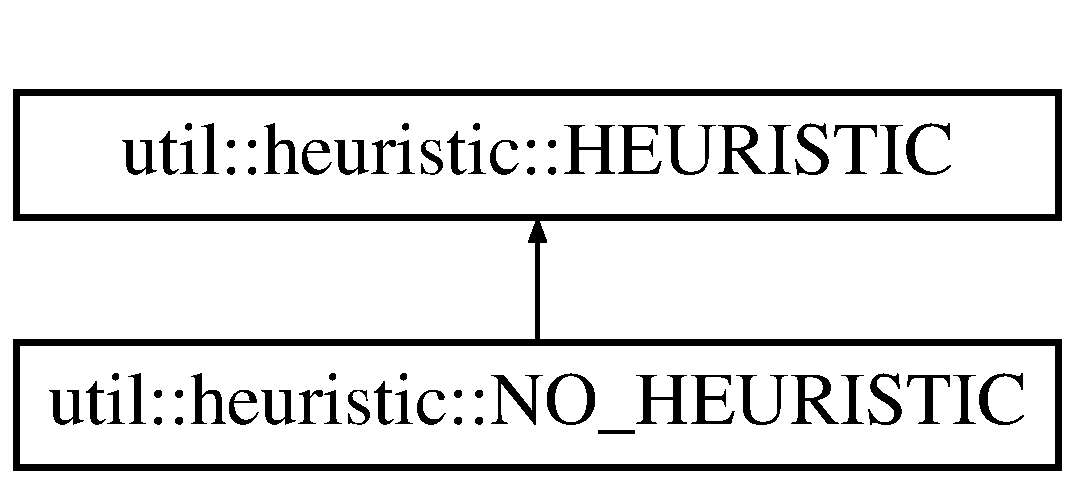
\includegraphics[height=2.000000cm]{structutil_1_1heuristic_1_1_n_o___h_e_u_r_i_s_t_i_c}
\end{center}
\end{figure}
\subsection*{Public Member Functions}
\begin{DoxyCompactItemize}
\item 
{\bfseries N\+O\+\_\+\+H\+E\+U\+R\+I\+S\+T\+IC} (\hyperlink{class_entity_system}{Entity\+System} \&ents)\hypertarget{structutil_1_1heuristic_1_1_n_o___h_e_u_r_i_s_t_i_c_ac8bf80b8fb6e6f5ddf3d3eb605bcf47d}{}\label{structutil_1_1heuristic_1_1_n_o___h_e_u_r_i_s_t_i_c_ac8bf80b8fb6e6f5ddf3d3eb605bcf47d}

\item 
tdt\+::real {\bfseries get\+\_\+cost} (tdt\+::uint id1, tdt\+::uint id2) override\hypertarget{structutil_1_1heuristic_1_1_n_o___h_e_u_r_i_s_t_i_c_a39e1b483a61ee4288a8f5bf18633f6c9}{}\label{structutil_1_1heuristic_1_1_n_o___h_e_u_r_i_s_t_i_c_a39e1b483a61ee4288a8f5bf18633f6c9}

\end{DoxyCompactItemize}
\subsection*{Additional Inherited Members}


\subsection{Detailed Description}
Represents no heuristic by returning 0 all the time. 

Definition at line 223 of file Pathfinding\+Algorithms.\+hpp.



The documentation for this struct was generated from the following file\+:\begin{DoxyCompactItemize}
\item 
tools/Pathfinding\+Algorithms.\+hpp\end{DoxyCompactItemize}

\hypertarget{struct_notification_component}{}\section{Notification\+Component Struct Reference}
\label{struct_notification_component}\index{Notification\+Component@{Notification\+Component}}


Allows to keep track about notification cooldown, so that an entity doesn\textquotesingle{}t spam the player with messages on reoccuring events in a short time period.  




{\ttfamily \#include $<$Components.\+hpp$>$}

\subsection*{Public Member Functions}
\begin{DoxyCompactItemize}
\item 
{\bfseries Notification\+Component} (tdt\+::real cd=0.f)\hypertarget{struct_notification_component_a61fe5bc08029f912e8d9750514feb10e}{}\label{struct_notification_component_a61fe5bc08029f912e8d9750514feb10e}

\item 
{\bfseries Notification\+Component} (const \hyperlink{struct_notification_component}{Notification\+Component} \&)=default\hypertarget{struct_notification_component_aa1a70a05af6e94956ae04495e93f50de}{}\label{struct_notification_component_aa1a70a05af6e94956ae04495e93f50de}

\item 
{\bfseries Notification\+Component} (\hyperlink{struct_notification_component}{Notification\+Component} \&\&)=default\hypertarget{struct_notification_component_ace3e34c0a180c7569a2c1b3d85313377}{}\label{struct_notification_component_ace3e34c0a180c7569a2c1b3d85313377}

\item 
\hyperlink{struct_notification_component}{Notification\+Component} \& {\bfseries operator=} (const \hyperlink{struct_notification_component}{Notification\+Component} \&)=default\hypertarget{struct_notification_component_add521cfd10be0b2ca8156f682048f25f}{}\label{struct_notification_component_add521cfd10be0b2ca8156f682048f25f}

\item 
\hyperlink{struct_notification_component}{Notification\+Component} \& {\bfseries operator=} (\hyperlink{struct_notification_component}{Notification\+Component} \&\&)=default\hypertarget{struct_notification_component_ae48f93cfc64db47efaa9111d7f7d5d45}{}\label{struct_notification_component_ae48f93cfc64db47efaa9111d7f7d5d45}

\end{DoxyCompactItemize}
\subsection*{Public Attributes}
\begin{DoxyCompactItemize}
\item 
tdt\+::real {\bfseries curr\+\_\+time}\hypertarget{struct_notification_component_a25bd9b213ce69c1a116172bf1260a297}{}\label{struct_notification_component_a25bd9b213ce69c1a116172bf1260a297}

\item 
tdt\+::real {\bfseries cooldown}\hypertarget{struct_notification_component_ab1ea5364d5028d54fbd1cdf5665116c4}{}\label{struct_notification_component_ab1ea5364d5028d54fbd1cdf5665116c4}

\end{DoxyCompactItemize}
\subsection*{Static Public Attributes}
\begin{DoxyCompactItemize}
\item 
static constexpr int {\bfseries type} = 31\hypertarget{struct_notification_component_ab08b754bf71f34e51e2627f916e4bcbc}{}\label{struct_notification_component_ab08b754bf71f34e51e2627f916e4bcbc}

\end{DoxyCompactItemize}


\subsection{Detailed Description}
Allows to keep track about notification cooldown, so that an entity doesn\textquotesingle{}t spam the player with messages on reoccuring events in a short time period. 

Definition at line 739 of file Components.\+hpp.



The documentation for this struct was generated from the following file\+:\begin{DoxyCompactItemize}
\item 
Components.\+hpp\end{DoxyCompactItemize}

\hypertarget{struct_on_hit_component}{}\section{On\+Hit\+Component Struct Reference}
\label{struct_on_hit_component}\index{On\+Hit\+Component@{On\+Hit\+Component}}


Contains the blueprint table which gets called when an entity that has this component gets hit.  




{\ttfamily \#include $<$Components.\+hpp$>$}

\subsection*{Public Member Functions}
\begin{DoxyCompactItemize}
\item 
{\bfseries On\+Hit\+Component} (std\+::string \&\&b=\char`\"{}E\+R\+R\+OR\char`\"{}, tdt\+::real cd=0.f)\hypertarget{struct_on_hit_component_ae624f7230c9650e7fa7c6b45cb7a8a49}{}\label{struct_on_hit_component_ae624f7230c9650e7fa7c6b45cb7a8a49}

\item 
{\bfseries On\+Hit\+Component} (const \hyperlink{struct_on_hit_component}{On\+Hit\+Component} \&)=default\hypertarget{struct_on_hit_component_a26ed54d5362548e20b05385c0f1c9f70}{}\label{struct_on_hit_component_a26ed54d5362548e20b05385c0f1c9f70}

\item 
{\bfseries On\+Hit\+Component} (\hyperlink{struct_on_hit_component}{On\+Hit\+Component} \&\&)=default\hypertarget{struct_on_hit_component_ade424965cf5910525d2a419533a57c86}{}\label{struct_on_hit_component_ade424965cf5910525d2a419533a57c86}

\item 
\hyperlink{struct_on_hit_component}{On\+Hit\+Component} \& {\bfseries operator=} (const \hyperlink{struct_on_hit_component}{On\+Hit\+Component} \&)=default\hypertarget{struct_on_hit_component_afed8a7f49f7592e6041eb074ad0bd46e}{}\label{struct_on_hit_component_afed8a7f49f7592e6041eb074ad0bd46e}

\item 
\hyperlink{struct_on_hit_component}{On\+Hit\+Component} \& {\bfseries operator=} (\hyperlink{struct_on_hit_component}{On\+Hit\+Component} \&\&)=default\hypertarget{struct_on_hit_component_af03cc5bbb044cf1f30beb7908248ff9e}{}\label{struct_on_hit_component_af03cc5bbb044cf1f30beb7908248ff9e}

\end{DoxyCompactItemize}
\subsection*{Public Attributes}
\begin{DoxyCompactItemize}
\item 
std\+::string {\bfseries blueprint}\hypertarget{struct_on_hit_component_a45ad4149f948fd41d7588bfa5ae58f37}{}\label{struct_on_hit_component_a45ad4149f948fd41d7588bfa5ae58f37}

\item 
tdt\+::real {\bfseries curr\+\_\+time}\hypertarget{struct_on_hit_component_adf4dc96c8f54b02e6b691c969af08939}{}\label{struct_on_hit_component_adf4dc96c8f54b02e6b691c969af08939}

\item 
tdt\+::real {\bfseries cooldown}\hypertarget{struct_on_hit_component_a3c8a85a54987f36f098692a8c7850309}{}\label{struct_on_hit_component_a3c8a85a54987f36f098692a8c7850309}

\end{DoxyCompactItemize}
\subsection*{Static Public Attributes}
\begin{DoxyCompactItemize}
\item 
static constexpr int {\bfseries type} = 27\hypertarget{struct_on_hit_component_a40e9cedb165528ed4b73832765266000}{}\label{struct_on_hit_component_a40e9cedb165528ed4b73832765266000}

\end{DoxyCompactItemize}


\subsection{Detailed Description}
Contains the blueprint table which gets called when an entity that has this component gets hit. 

Definition at line 647 of file Components.\+hpp.



The documentation for this struct was generated from the following file\+:\begin{DoxyCompactItemize}
\item 
Components.\+hpp\end{DoxyCompactItemize}

\hypertarget{class_options_window}{}\section{Options\+Window Class Reference}
\label{class_options_window}\index{Options\+Window@{Options\+Window}}


Options menu window that lets the player to change the resolution, window mode and keybinging.  




{\ttfamily \#include $<$Options\+Window.\+hpp$>$}

Inheritance diagram for Options\+Window\+:\begin{figure}[H]
\begin{center}
\leavevmode
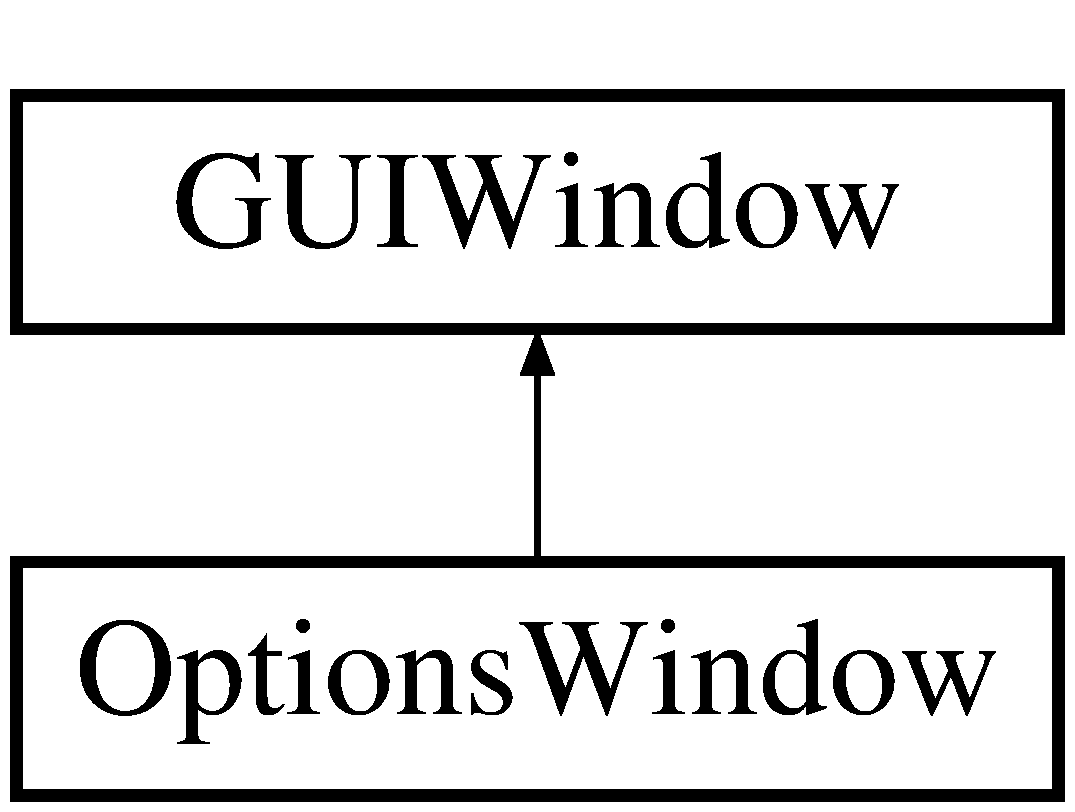
\includegraphics[height=2.000000cm]{class_options_window}
\end{center}
\end{figure}
\subsection*{Public Member Functions}
\begin{DoxyCompactItemize}
\item 
\hyperlink{class_options_window_a83990c03d2fec467c1131d7961f59e25}{Options\+Window} ()
\begin{DoxyCompactList}\small\item\em Constructor. \end{DoxyCompactList}\item 
\hyperlink{class_options_window_a4937f89a05eedf7bc9122b8df37ff805}{$\sim$\+Options\+Window} ()=default
\begin{DoxyCompactList}\small\item\em Destructor. \end{DoxyCompactList}\item 
void \hyperlink{class_options_window_ac629faa5a25c78141897ab2f53ec9bb4}{add\+\_\+start\+\_\+parameters} (Ogre\+::\+Render\+Window $\ast$, Ogre\+::\+Viewport $\ast$, C\+E\+G\+U\+I\+::\+Ogre\+Renderer $\ast$)
\begin{DoxyCompactList}\small\item\em Saves pointers to the window, view and renderer and sets starting values for the resolution, window mode etc. \end{DoxyCompactList}\item 
bool \hyperlink{class_options_window_a35feca3b435b2205f72138f65d20cf5d}{key\+\_\+pressed} (C\+E\+G\+U\+I\+::\+Key\+::\+Scan)
\begin{DoxyCompactList}\small\item\em Registers a key press for keybinding. \end{DoxyCompactList}\item 
void \hyperlink{class_options_window_af171624435787e543e9dcb64b5bce39e}{set\+\_\+key\+\_\+bind} (K\+E\+Y\+\_\+\+B\+I\+N\+D\+\_\+\+A\+C\+T\+I\+O\+N\+::\+V\+AL, C\+E\+G\+U\+I\+::\+Key\+::\+Scan)
\begin{DoxyCompactList}\small\item\em Binds a given action to a given key. \end{DoxyCompactList}\end{DoxyCompactItemize}
\subsection*{Protected Member Functions}
\begin{DoxyCompactItemize}
\item 
void \hyperlink{class_options_window_a88bfc1401a1113e4ab4afdb8af106682}{init\+\_\+} () override
\begin{DoxyCompactList}\small\item\em Initializes the C\+E\+G\+UI window. \end{DoxyCompactList}\end{DoxyCompactItemize}
\subsection*{Private Types}
\begin{DoxyCompactItemize}
\item 
typedef void($\ast$ {\bfseries Action\+Func\+Ptr}) ()\hypertarget{class_options_window_a5f01e3cb1c649c429ff4e8f3cfeda350}{}\label{class_options_window_a5f01e3cb1c649c429ff4e8f3cfeda350}

\end{DoxyCompactItemize}
\subsection*{Private Member Functions}
\begin{DoxyCompactItemize}
\item 
void \hyperlink{class_options_window_a4bde7704e95b5ee4fb80bbf2b325c16b}{apply\+\_\+} ()
\begin{DoxyCompactList}\small\item\em Applies the graphical changes and saves key bindings into a script that allows persistent key binds. \end{DoxyCompactList}\item 
void \hyperlink{class_options_window_a357e35144c8067c54cd12907dd11417b}{update\+\_\+labels\+\_\+} ()
\begin{DoxyCompactList}\small\item\em Updates the button texts and labels to reflect the new settings. \end{DoxyCompactList}\item 
void {\bfseries update\+\_\+fonts\+\_\+} ()\hypertarget{class_options_window_ab1629d4e6c35737a8e7588d1ce99fb5d}{}\label{class_options_window_ab1629d4e6c35737a8e7588d1ce99fb5d}

\item 
void {\bfseries update\+\_\+font\+\_\+of\+\_\+window\+\_\+} (C\+E\+G\+U\+I\+::\+Window $\ast$, const std\+::string \&)\hypertarget{class_options_window_acfebf79f3daf208868565b185634e641}{}\label{class_options_window_acfebf79f3daf208868565b185634e641}

\item 
const std\+::string \& \hyperlink{class_options_window_a949bdb318ae5834f72eb906076941842}{get\+\_\+key\+\_\+bind\+\_\+name\+\_\+} (K\+E\+Y\+\_\+\+B\+I\+N\+D\+\_\+\+A\+C\+T\+I\+O\+N\+::\+V\+AL)
\begin{DoxyCompactList}\small\item\em Returns the name of the key a given action is bound to. \end{DoxyCompactList}\end{DoxyCompactItemize}
\subsection*{Private Attributes}
\begin{DoxyCompactItemize}
\item 
Ogre\+::\+Render\+Window $\ast$ \hyperlink{class_options_window_a9c6b55b36d1f57ea60885cf0a59291ca}{render\+\_\+window\+\_\+}
\begin{DoxyCompactList}\small\item\em Window the game is rendered to. \end{DoxyCompactList}\item 
Ogre\+::\+Viewport $\ast$ \hyperlink{class_options_window_a8c3609894e71264da13b88129d0a1f70}{view\+\_\+}
\begin{DoxyCompactList}\small\item\em Main viewport of the render window. \end{DoxyCompactList}\item 
C\+E\+G\+U\+I\+::\+Ogre\+Renderer $\ast$ \hyperlink{class_options_window_aa46c54f3e0956dce55fb370324d91772}{renderer\+\_\+}
\begin{DoxyCompactList}\small\item\em Renderer used by C\+E\+G\+UI (used to sync resolution between game and UI). \end{DoxyCompactList}\item 
tdt\+::uint \hyperlink{class_options_window_ab5b2b96bd284265c5a49b145493e8ead}{width\+\_\+}
\begin{DoxyCompactList}\small\item\em Dimensions of the display resolution. \end{DoxyCompactList}\item 
tdt\+::uint {\bfseries height\+\_\+}\hypertarget{class_options_window_aa2b6e26908f2ee947a997d76de66cc6f}{}\label{class_options_window_aa2b6e26908f2ee947a997d76de66cc6f}

\item 
bool \hyperlink{class_options_window_a536d5e2d5cc3f8c419836e1e5ff80423}{fullscreen\+\_\+}
\begin{DoxyCompactList}\small\item\em True for fullscreen, false for windowed mode. \end{DoxyCompactList}\item 
std\+::map$<$ C\+E\+G\+U\+I\+::\+Key\+::\+Scan, std\+::string $>$ \hyperlink{class_options_window_a65c8541c815655feaa458edb01738213}{key\+\_\+names\+\_\+}
\begin{DoxyCompactList}\small\item\em This map connects key codes with their names (used for key bind buttons). \end{DoxyCompactList}\item 
std\+::array$<$ Action\+Func\+Ptr, K\+E\+Y\+\_\+\+B\+I\+N\+D\+\_\+\+A\+C\+T\+I\+O\+N\+::\+C\+O\+U\+NT $>$ \hyperlink{class_options_window_a343bc2c957774fb3de4ba8ea8fbef3df}{actions\+\_\+}
\begin{DoxyCompactList}\small\item\em Action functions assigned to actions. \end{DoxyCompactList}\item 
std\+::array$<$ C\+E\+G\+U\+I\+::\+Key\+::\+Scan, K\+E\+Y\+\_\+\+B\+I\+N\+D\+\_\+\+A\+C\+T\+I\+O\+N\+::\+C\+O\+U\+NT $>$ \hyperlink{class_options_window_a1727e50166ba8b67f5f97f6213e0f80d}{key\+\_\+binds\+\_\+}
\begin{DoxyCompactList}\small\item\em Keys bound to actions. \end{DoxyCompactList}\item 
std\+::map$<$ std\+::string, std\+::tuple$<$ tdt\+::uint, tdt\+::uint $>$ $>$ \hyperlink{class_options_window_ae7e2ff101e41b90c0063b78710b85639}{resolutions\+\_\+}
\begin{DoxyCompactList}\small\item\em Resolution strings and their assigned dimensions. \end{DoxyCompactList}\item 
K\+E\+Y\+\_\+\+B\+I\+N\+D\+\_\+\+A\+C\+T\+I\+O\+N\+::\+V\+AL \hyperlink{class_options_window_a62f3d533394c12986766deb0e73794c2}{currently\+\_\+binded\+\_\+action\+\_\+}
\begin{DoxyCompactList}\small\item\em Saves the currently binded action so that the next key press can be used. \end{DoxyCompactList}\end{DoxyCompactItemize}
\subsection*{Additional Inherited Members}


\subsection{Detailed Description}
Options menu window that lets the player to change the resolution, window mode and keybinging. 

Definition at line 18 of file Options\+Window.\+hpp.



\subsection{Constructor \& Destructor Documentation}
\index{Options\+Window@{Options\+Window}!Options\+Window@{Options\+Window}}
\index{Options\+Window@{Options\+Window}!Options\+Window@{Options\+Window}}
\subsubsection[{\texorpdfstring{Options\+Window()}{OptionsWindow()}}]{\setlength{\rightskip}{0pt plus 5cm}Options\+Window\+::\+Options\+Window (
\begin{DoxyParamCaption}
{}
\end{DoxyParamCaption}
)}\hypertarget{class_options_window_a83990c03d2fec467c1131d7961f59e25}{}\label{class_options_window_a83990c03d2fec467c1131d7961f59e25}


Constructor. 



Definition at line 8 of file Options\+Window.\+cpp.

\index{Options\+Window@{Options\+Window}!````~Options\+Window@{$\sim$\+Options\+Window}}
\index{````~Options\+Window@{$\sim$\+Options\+Window}!Options\+Window@{Options\+Window}}
\subsubsection[{\texorpdfstring{$\sim$\+Options\+Window()=default}{~OptionsWindow()=default}}]{\setlength{\rightskip}{0pt plus 5cm}Options\+Window\+::$\sim$\+Options\+Window (
\begin{DoxyParamCaption}
{}
\end{DoxyParamCaption}
)\hspace{0.3cm}{\ttfamily [default]}}\hypertarget{class_options_window_a4937f89a05eedf7bc9122b8df37ff805}{}\label{class_options_window_a4937f89a05eedf7bc9122b8df37ff805}


Destructor. 



\subsection{Member Function Documentation}
\index{Options\+Window@{Options\+Window}!add\+\_\+start\+\_\+parameters@{add\+\_\+start\+\_\+parameters}}
\index{add\+\_\+start\+\_\+parameters@{add\+\_\+start\+\_\+parameters}!Options\+Window@{Options\+Window}}
\subsubsection[{\texorpdfstring{add\+\_\+start\+\_\+parameters(\+Ogre\+::\+Render\+Window $\ast$, Ogre\+::\+Viewport $\ast$, C\+E\+G\+U\+I\+::\+Ogre\+Renderer $\ast$)}{add_start_parameters(Ogre::RenderWindow *, Ogre::Viewport *, CEGUI::OgreRenderer *)}}]{\setlength{\rightskip}{0pt plus 5cm}void Options\+Window\+::add\+\_\+start\+\_\+parameters (
\begin{DoxyParamCaption}
\item[{Ogre\+::\+Render\+Window $\ast$}]{window, }
\item[{Ogre\+::\+Viewport $\ast$}]{view, }
\item[{C\+E\+G\+U\+I\+::\+Ogre\+Renderer $\ast$}]{renderer}
\end{DoxyParamCaption}
)}\hypertarget{class_options_window_ac629faa5a25c78141897ab2f53ec9bb4}{}\label{class_options_window_ac629faa5a25c78141897ab2f53ec9bb4}


Saves pointers to the window, view and renderer and sets starting values for the resolution, window mode etc. 


\begin{DoxyParams}{Parameters}
{\em Window} & that the game is rendered to. \\
\hline
{\em Viewport} & of the window. \\
\hline
{\em Renderer} & used by C\+E\+G\+UI. \\
\hline
\end{DoxyParams}


Definition at line 13 of file Options\+Window.\+cpp.

\index{Options\+Window@{Options\+Window}!apply\+\_\+@{apply\+\_\+}}
\index{apply\+\_\+@{apply\+\_\+}!Options\+Window@{Options\+Window}}
\subsubsection[{\texorpdfstring{apply\+\_\+()}{apply_()}}]{\setlength{\rightskip}{0pt plus 5cm}void Options\+Window\+::apply\+\_\+ (
\begin{DoxyParamCaption}
{}
\end{DoxyParamCaption}
)\hspace{0.3cm}{\ttfamily [private]}}\hypertarget{class_options_window_a4bde7704e95b5ee4fb80bbf2b325c16b}{}\label{class_options_window_a4bde7704e95b5ee4fb80bbf2b325c16b}


Applies the graphical changes and saves key bindings into a script that allows persistent key binds. 

This will make sure that key bindings are persistent.

Definition at line 307 of file Options\+Window.\+cpp.

\index{Options\+Window@{Options\+Window}!get\+\_\+key\+\_\+bind\+\_\+name\+\_\+@{get\+\_\+key\+\_\+bind\+\_\+name\+\_\+}}
\index{get\+\_\+key\+\_\+bind\+\_\+name\+\_\+@{get\+\_\+key\+\_\+bind\+\_\+name\+\_\+}!Options\+Window@{Options\+Window}}
\subsubsection[{\texorpdfstring{get\+\_\+key\+\_\+bind\+\_\+name\+\_\+(\+K\+E\+Y\+\_\+\+B\+I\+N\+D\+\_\+\+A\+C\+T\+I\+O\+N\+::\+V\+A\+L)}{get_key_bind_name_(KEY_BIND_ACTION::VAL)}}]{\setlength{\rightskip}{0pt plus 5cm}const std\+::string \& Options\+Window\+::get\+\_\+key\+\_\+bind\+\_\+name\+\_\+ (
\begin{DoxyParamCaption}
\item[{K\+E\+Y\+\_\+\+B\+I\+N\+D\+\_\+\+A\+C\+T\+I\+O\+N\+::\+V\+AL}]{action}
\end{DoxyParamCaption}
)\hspace{0.3cm}{\ttfamily [private]}}\hypertarget{class_options_window_a949bdb318ae5834f72eb906076941842}{}\label{class_options_window_a949bdb318ae5834f72eb906076941842}


Returns the name of the key a given action is bound to. 


\begin{DoxyParams}{Parameters}
{\em The} & action. \\
\hline
\end{DoxyParams}


Definition at line 425 of file Options\+Window.\+cpp.

\index{Options\+Window@{Options\+Window}!init\+\_\+@{init\+\_\+}}
\index{init\+\_\+@{init\+\_\+}!Options\+Window@{Options\+Window}}
\subsubsection[{\texorpdfstring{init\+\_\+() override}{init_() override}}]{\setlength{\rightskip}{0pt plus 5cm}void Options\+Window\+::init\+\_\+ (
\begin{DoxyParamCaption}
{}
\end{DoxyParamCaption}
)\hspace{0.3cm}{\ttfamily [override]}, {\ttfamily [protected]}, {\ttfamily [virtual]}}\hypertarget{class_options_window_a88bfc1401a1113e4ab4afdb8af106682}{}\label{class_options_window_a88bfc1401a1113e4ab4afdb8af106682}


Initializes the C\+E\+G\+UI window. 



Implements \hyperlink{class_g_u_i_window_a2a7c011363f401a57a26cc7c7652bdfd}{G\+U\+I\+Window}.



Definition at line 64 of file Options\+Window.\+cpp.

\index{Options\+Window@{Options\+Window}!key\+\_\+pressed@{key\+\_\+pressed}}
\index{key\+\_\+pressed@{key\+\_\+pressed}!Options\+Window@{Options\+Window}}
\subsubsection[{\texorpdfstring{key\+\_\+pressed(\+C\+E\+G\+U\+I\+::\+Key\+::\+Scan)}{key_pressed(CEGUI::Key::Scan)}}]{\setlength{\rightskip}{0pt plus 5cm}bool Options\+Window\+::key\+\_\+pressed (
\begin{DoxyParamCaption}
\item[{C\+E\+G\+U\+I\+::\+Key\+::\+Scan}]{key}
\end{DoxyParamCaption}
)}\hypertarget{class_options_window_a35feca3b435b2205f72138f65d20cf5d}{}\label{class_options_window_a35feca3b435b2205f72138f65d20cf5d}


Registers a key press for keybinding. 

Returns true if the click was consumed, false otherwise. 
\begin{DoxyParams}{Parameters}
{\em Key} & pressed. \\
\hline
\end{DoxyParams}


Definition at line 26 of file Options\+Window.\+cpp.

\index{Options\+Window@{Options\+Window}!set\+\_\+key\+\_\+bind@{set\+\_\+key\+\_\+bind}}
\index{set\+\_\+key\+\_\+bind@{set\+\_\+key\+\_\+bind}!Options\+Window@{Options\+Window}}
\subsubsection[{\texorpdfstring{set\+\_\+key\+\_\+bind(\+K\+E\+Y\+\_\+\+B\+I\+N\+D\+\_\+\+A\+C\+T\+I\+O\+N\+::\+V\+A\+L, C\+E\+G\+U\+I\+::\+Key\+::\+Scan)}{set_key_bind(KEY_BIND_ACTION::VAL, CEGUI::Key::Scan)}}]{\setlength{\rightskip}{0pt plus 5cm}void Options\+Window\+::set\+\_\+key\+\_\+bind (
\begin{DoxyParamCaption}
\item[{K\+E\+Y\+\_\+\+B\+I\+N\+D\+\_\+\+A\+C\+T\+I\+O\+N\+::\+V\+AL}]{action, }
\item[{C\+E\+G\+U\+I\+::\+Key\+::\+Scan}]{key}
\end{DoxyParamCaption}
)}\hypertarget{class_options_window_af171624435787e543e9dcb64b5bce39e}{}\label{class_options_window_af171624435787e543e9dcb64b5bce39e}


Binds a given action to a given key. 


\begin{DoxyParams}{Parameters}
{\em Action} & to be bound. \\
\hline
{\em Key} & to be bound. \\
\hline
\end{DoxyParams}


Definition at line 58 of file Options\+Window.\+cpp.

\index{Options\+Window@{Options\+Window}!update\+\_\+labels\+\_\+@{update\+\_\+labels\+\_\+}}
\index{update\+\_\+labels\+\_\+@{update\+\_\+labels\+\_\+}!Options\+Window@{Options\+Window}}
\subsubsection[{\texorpdfstring{update\+\_\+labels\+\_\+()}{update_labels_()}}]{\setlength{\rightskip}{0pt plus 5cm}void Options\+Window\+::update\+\_\+labels\+\_\+ (
\begin{DoxyParamCaption}
{}
\end{DoxyParamCaption}
)\hspace{0.3cm}{\ttfamily [private]}}\hypertarget{class_options_window_a357e35144c8067c54cd12907dd11417b}{}\label{class_options_window_a357e35144c8067c54cd12907dd11417b}


Updates the button texts and labels to reflect the new settings. 



Definition at line 348 of file Options\+Window.\+cpp.



\subsection{Member Data Documentation}
\index{Options\+Window@{Options\+Window}!actions\+\_\+@{actions\+\_\+}}
\index{actions\+\_\+@{actions\+\_\+}!Options\+Window@{Options\+Window}}
\subsubsection[{\texorpdfstring{actions\+\_\+}{actions_}}]{\setlength{\rightskip}{0pt plus 5cm}std\+::array$<$Action\+Func\+Ptr, K\+E\+Y\+\_\+\+B\+I\+N\+D\+\_\+\+A\+C\+T\+I\+O\+N\+::\+C\+O\+U\+NT$>$ Options\+Window\+::actions\+\_\+\hspace{0.3cm}{\ttfamily [private]}}\hypertarget{class_options_window_a343bc2c957774fb3de4ba8ea8fbef3df}{}\label{class_options_window_a343bc2c957774fb3de4ba8ea8fbef3df}


Action functions assigned to actions. 



Definition at line 124 of file Options\+Window.\+hpp.

\index{Options\+Window@{Options\+Window}!currently\+\_\+binded\+\_\+action\+\_\+@{currently\+\_\+binded\+\_\+action\+\_\+}}
\index{currently\+\_\+binded\+\_\+action\+\_\+@{currently\+\_\+binded\+\_\+action\+\_\+}!Options\+Window@{Options\+Window}}
\subsubsection[{\texorpdfstring{currently\+\_\+binded\+\_\+action\+\_\+}{currently_binded_action_}}]{\setlength{\rightskip}{0pt plus 5cm}K\+E\+Y\+\_\+\+B\+I\+N\+D\+\_\+\+A\+C\+T\+I\+O\+N\+::\+V\+AL Options\+Window\+::currently\+\_\+binded\+\_\+action\+\_\+\hspace{0.3cm}{\ttfamily [private]}}\hypertarget{class_options_window_a62f3d533394c12986766deb0e73794c2}{}\label{class_options_window_a62f3d533394c12986766deb0e73794c2}


Saves the currently binded action so that the next key press can be used. 



Definition at line 140 of file Options\+Window.\+hpp.

\index{Options\+Window@{Options\+Window}!fullscreen\+\_\+@{fullscreen\+\_\+}}
\index{fullscreen\+\_\+@{fullscreen\+\_\+}!Options\+Window@{Options\+Window}}
\subsubsection[{\texorpdfstring{fullscreen\+\_\+}{fullscreen_}}]{\setlength{\rightskip}{0pt plus 5cm}bool Options\+Window\+::fullscreen\+\_\+\hspace{0.3cm}{\ttfamily [private]}}\hypertarget{class_options_window_a536d5e2d5cc3f8c419836e1e5ff80423}{}\label{class_options_window_a536d5e2d5cc3f8c419836e1e5ff80423}


True for fullscreen, false for windowed mode. 



Definition at line 114 of file Options\+Window.\+hpp.

\index{Options\+Window@{Options\+Window}!key\+\_\+binds\+\_\+@{key\+\_\+binds\+\_\+}}
\index{key\+\_\+binds\+\_\+@{key\+\_\+binds\+\_\+}!Options\+Window@{Options\+Window}}
\subsubsection[{\texorpdfstring{key\+\_\+binds\+\_\+}{key_binds_}}]{\setlength{\rightskip}{0pt plus 5cm}std\+::array$<$C\+E\+G\+U\+I\+::\+Key\+::\+Scan, K\+E\+Y\+\_\+\+B\+I\+N\+D\+\_\+\+A\+C\+T\+I\+O\+N\+::\+C\+O\+U\+NT$>$ Options\+Window\+::key\+\_\+binds\+\_\+\hspace{0.3cm}{\ttfamily [private]}}\hypertarget{class_options_window_a1727e50166ba8b67f5f97f6213e0f80d}{}\label{class_options_window_a1727e50166ba8b67f5f97f6213e0f80d}


Keys bound to actions. 



Definition at line 129 of file Options\+Window.\+hpp.

\index{Options\+Window@{Options\+Window}!key\+\_\+names\+\_\+@{key\+\_\+names\+\_\+}}
\index{key\+\_\+names\+\_\+@{key\+\_\+names\+\_\+}!Options\+Window@{Options\+Window}}
\subsubsection[{\texorpdfstring{key\+\_\+names\+\_\+}{key_names_}}]{\setlength{\rightskip}{0pt plus 5cm}std\+::map$<$C\+E\+G\+U\+I\+::\+Key\+::\+Scan, std\+::string$>$ Options\+Window\+::key\+\_\+names\+\_\+\hspace{0.3cm}{\ttfamily [private]}}\hypertarget{class_options_window_a65c8541c815655feaa458edb01738213}{}\label{class_options_window_a65c8541c815655feaa458edb01738213}


This map connects key codes with their names (used for key bind buttons). 



Definition at line 119 of file Options\+Window.\+hpp.

\index{Options\+Window@{Options\+Window}!render\+\_\+window\+\_\+@{render\+\_\+window\+\_\+}}
\index{render\+\_\+window\+\_\+@{render\+\_\+window\+\_\+}!Options\+Window@{Options\+Window}}
\subsubsection[{\texorpdfstring{render\+\_\+window\+\_\+}{render_window_}}]{\setlength{\rightskip}{0pt plus 5cm}Ogre\+::\+Render\+Window$\ast$ Options\+Window\+::render\+\_\+window\+\_\+\hspace{0.3cm}{\ttfamily [private]}}\hypertarget{class_options_window_a9c6b55b36d1f57ea60885cf0a59291ca}{}\label{class_options_window_a9c6b55b36d1f57ea60885cf0a59291ca}


Window the game is rendered to. 



Definition at line 94 of file Options\+Window.\+hpp.

\index{Options\+Window@{Options\+Window}!renderer\+\_\+@{renderer\+\_\+}}
\index{renderer\+\_\+@{renderer\+\_\+}!Options\+Window@{Options\+Window}}
\subsubsection[{\texorpdfstring{renderer\+\_\+}{renderer_}}]{\setlength{\rightskip}{0pt plus 5cm}C\+E\+G\+U\+I\+::\+Ogre\+Renderer$\ast$ Options\+Window\+::renderer\+\_\+\hspace{0.3cm}{\ttfamily [private]}}\hypertarget{class_options_window_aa46c54f3e0956dce55fb370324d91772}{}\label{class_options_window_aa46c54f3e0956dce55fb370324d91772}


Renderer used by C\+E\+G\+UI (used to sync resolution between game and UI). 



Definition at line 104 of file Options\+Window.\+hpp.

\index{Options\+Window@{Options\+Window}!resolutions\+\_\+@{resolutions\+\_\+}}
\index{resolutions\+\_\+@{resolutions\+\_\+}!Options\+Window@{Options\+Window}}
\subsubsection[{\texorpdfstring{resolutions\+\_\+}{resolutions_}}]{\setlength{\rightskip}{0pt plus 5cm}std\+::map$<$std\+::string, std\+::tuple$<$tdt\+::uint, tdt\+::uint$>$ $>$ Options\+Window\+::resolutions\+\_\+\hspace{0.3cm}{\ttfamily [private]}}\hypertarget{class_options_window_ae7e2ff101e41b90c0063b78710b85639}{}\label{class_options_window_ae7e2ff101e41b90c0063b78710b85639}


Resolution strings and their assigned dimensions. 



Definition at line 134 of file Options\+Window.\+hpp.

\index{Options\+Window@{Options\+Window}!view\+\_\+@{view\+\_\+}}
\index{view\+\_\+@{view\+\_\+}!Options\+Window@{Options\+Window}}
\subsubsection[{\texorpdfstring{view\+\_\+}{view_}}]{\setlength{\rightskip}{0pt plus 5cm}Ogre\+::\+Viewport$\ast$ Options\+Window\+::view\+\_\+\hspace{0.3cm}{\ttfamily [private]}}\hypertarget{class_options_window_a8c3609894e71264da13b88129d0a1f70}{}\label{class_options_window_a8c3609894e71264da13b88129d0a1f70}


Main viewport of the render window. 



Definition at line 99 of file Options\+Window.\+hpp.

\index{Options\+Window@{Options\+Window}!width\+\_\+@{width\+\_\+}}
\index{width\+\_\+@{width\+\_\+}!Options\+Window@{Options\+Window}}
\subsubsection[{\texorpdfstring{width\+\_\+}{width_}}]{\setlength{\rightskip}{0pt plus 5cm}tdt\+::uint Options\+Window\+::width\+\_\+\hspace{0.3cm}{\ttfamily [private]}}\hypertarget{class_options_window_ab5b2b96bd284265c5a49b145493e8ead}{}\label{class_options_window_ab5b2b96bd284265c5a49b145493e8ead}


Dimensions of the display resolution. 



Definition at line 109 of file Options\+Window.\+hpp.



The documentation for this class was generated from the following files\+:\begin{DoxyCompactItemize}
\item 
gui/Options\+Window.\+hpp\item 
gui/Options\+Window.\+cpp\end{DoxyCompactItemize}

\hypertarget{struct_pathfinding_component}{}\section{Pathfinding\+Component Struct Reference}
\label{struct_pathfinding_component}\index{Pathfinding\+Component@{Pathfinding\+Component}}


Holds data related to the entity\textquotesingle{}s current path.  




{\ttfamily \#include $<$Components.\+hpp$>$}

\subsection*{Public Member Functions}
\begin{DoxyCompactItemize}
\item 
{\bfseries Pathfinding\+Component} (std\+::string \&\&b=\char`\"{}E\+R\+R\+OR\char`\"{}, tdt\+::uint tar=0, tdt\+::uint last=0)\hypertarget{struct_pathfinding_component_a9be793c07176b14d62be3a1eaf67d12f}{}\label{struct_pathfinding_component_a9be793c07176b14d62be3a1eaf67d12f}

\item 
{\bfseries Pathfinding\+Component} (const \hyperlink{struct_pathfinding_component}{Pathfinding\+Component} \&)=default\hypertarget{struct_pathfinding_component_ac24b51a4f9b35e19fa96ede4ea394fb6}{}\label{struct_pathfinding_component_ac24b51a4f9b35e19fa96ede4ea394fb6}

\item 
{\bfseries Pathfinding\+Component} (\hyperlink{struct_pathfinding_component}{Pathfinding\+Component} \&\&)=default\hypertarget{struct_pathfinding_component_aafbee1831f248a6db84d49c1c482dd4e}{}\label{struct_pathfinding_component_aafbee1831f248a6db84d49c1c482dd4e}

\item 
\hyperlink{struct_pathfinding_component}{Pathfinding\+Component} \& {\bfseries operator=} (const \hyperlink{struct_pathfinding_component}{Pathfinding\+Component} \&)=default\hypertarget{struct_pathfinding_component_a6f4639a658f67253925ab28d3b7b35da}{}\label{struct_pathfinding_component_a6f4639a658f67253925ab28d3b7b35da}

\item 
\hyperlink{struct_pathfinding_component}{Pathfinding\+Component} \& {\bfseries operator=} (\hyperlink{struct_pathfinding_component}{Pathfinding\+Component} \&\&)=default\hypertarget{struct_pathfinding_component_a2c0bda4c5ac1493882bb9bbce141eebb}{}\label{struct_pathfinding_component_a2c0bda4c5ac1493882bb9bbce141eebb}

\end{DoxyCompactItemize}
\subsection*{Public Attributes}
\begin{DoxyCompactItemize}
\item 
tdt\+::uint {\bfseries target\+\_\+id}\hypertarget{struct_pathfinding_component_a702c1d838c506aed0f3cd53d3f3ebb65}{}\label{struct_pathfinding_component_a702c1d838c506aed0f3cd53d3f3ebb65}

\item 
tdt\+::uint {\bfseries last\+\_\+id}\hypertarget{struct_pathfinding_component_a1daf41de8bc5482685438a17a3468b99}{}\label{struct_pathfinding_component_a1daf41de8bc5482685438a17a3468b99}

\item 
std\+::deque$<$ tdt\+::uint $>$ {\bfseries path\+\_\+queue}\hypertarget{struct_pathfinding_component_ae4c40d5450a651ed5ba379f64dee4da2}{}\label{struct_pathfinding_component_ae4c40d5450a651ed5ba379f64dee4da2}

\item 
std\+::string {\bfseries blueprint}\hypertarget{struct_pathfinding_component_a52000821d45f0fef9e1393d4a43d2747}{}\label{struct_pathfinding_component_a52000821d45f0fef9e1393d4a43d2747}

\end{DoxyCompactItemize}
\subsection*{Static Public Attributes}
\begin{DoxyCompactItemize}
\item 
static constexpr int {\bfseries type} = 14\hypertarget{struct_pathfinding_component_a24b75510a249b07034b96bd6d4524c58}{}\label{struct_pathfinding_component_a24b75510a249b07034b96bd6d4524c58}

\end{DoxyCompactItemize}


\subsection{Detailed Description}
Holds data related to the entity\textquotesingle{}s current path. 

Definition at line 367 of file Components.\+hpp.



The documentation for this struct was generated from the following file\+:\begin{DoxyCompactItemize}
\item 
Components.\+hpp\end{DoxyCompactItemize}

\hypertarget{struct_physics_component}{}\section{Physics\+Component Struct Reference}
\label{struct_physics_component}\index{Physics\+Component@{Physics\+Component}}


Components.  




{\ttfamily \#include $<$Components.\+hpp$>$}

\subsection*{Public Member Functions}
\begin{DoxyCompactItemize}
\item 
{\bfseries Physics\+Component} (bool s=false, Ogre\+::\+Vector3 pos=Ogre\+::\+Vector3\{0, 0, 0\}, tdt\+::real hh=0.f)\hypertarget{struct_physics_component_ab1cb618d94011e593f1c522a7485f878}{}\label{struct_physics_component_ab1cb618d94011e593f1c522a7485f878}

\item 
{\bfseries Physics\+Component} (const \hyperlink{struct_physics_component}{Physics\+Component} \&)=default\hypertarget{struct_physics_component_ad1253f440a9d3cd2199a91a5f0371dd9}{}\label{struct_physics_component_ad1253f440a9d3cd2199a91a5f0371dd9}

\item 
{\bfseries Physics\+Component} (\hyperlink{struct_physics_component}{Physics\+Component} \&\&)=default\hypertarget{struct_physics_component_ac9387a296d252e63021a03ca66bfffdc}{}\label{struct_physics_component_ac9387a296d252e63021a03ca66bfffdc}

\item 
\hyperlink{struct_physics_component}{Physics\+Component} \& {\bfseries operator=} (const \hyperlink{struct_physics_component}{Physics\+Component} \&)=default\hypertarget{struct_physics_component_a83a73045999afdafb0ec5b1ee803e025}{}\label{struct_physics_component_a83a73045999afdafb0ec5b1ee803e025}

\item 
\hyperlink{struct_physics_component}{Physics\+Component} \& {\bfseries operator=} (\hyperlink{struct_physics_component}{Physics\+Component} \&\&)=default\hypertarget{struct_physics_component_a1b9671d67f08794d09b1577fe45ec9f9}{}\label{struct_physics_component_a1b9671d67f08794d09b1577fe45ec9f9}

\end{DoxyCompactItemize}
\subsection*{Public Attributes}
\begin{DoxyCompactItemize}
\item 
bool {\bfseries solid}\hypertarget{struct_physics_component_a242dde7c1239f5379b3498e628bb0977}{}\label{struct_physics_component_a242dde7c1239f5379b3498e628bb0977}

\item 
Ogre\+::\+Vector3 {\bfseries position}\hypertarget{struct_physics_component_ac550fbdeaabe49e502568b002df93d02}{}\label{struct_physics_component_ac550fbdeaabe49e502568b002df93d02}

\item 
tdt\+::real {\bfseries half\+\_\+height}\hypertarget{struct_physics_component_a6336b8ed7ecfc662bc296d13fb4b9bc1}{}\label{struct_physics_component_a6336b8ed7ecfc662bc296d13fb4b9bc1}

\end{DoxyCompactItemize}
\subsection*{Static Public Attributes}
\begin{DoxyCompactItemize}
\item 
static constexpr int {\bfseries type} = 0\hypertarget{struct_physics_component_aa3503fc9f153c589bc1d355f62a36299}{}\label{struct_physics_component_aa3503fc9f153c589bc1d355f62a36299}

\end{DoxyCompactItemize}


\subsection{Detailed Description}
Components. 

\begin{DoxyNote}{Note}
To be able to manually create components without blueprints, all components must have either default constructors or constructors with default values for all parameters, to be able to back components up, they need to provide a copy constructor. 

As constructors are called in the \hyperlink{class_entity_system_ac2d122f65e967b51cc37227b5dd0a7fe}{Entity\+System\+::load\+\_\+component} function, strings will be read from Lua and immediately discarded. Hence it was decided to make the string parameters accepted as rvalues for faster construction. Holds info related to physical interaction of an entity with the rest of the game world. 
\end{DoxyNote}


Definition at line 34 of file Components.\+hpp.



The documentation for this struct was generated from the following file\+:\begin{DoxyCompactItemize}
\item 
Components.\+hpp\end{DoxyCompactItemize}

\hypertarget{class_player}{}\section{Player Class Reference}
\label{class_player}\index{Player@{Player}}


Auxiliary class representing the player\textquotesingle{}s resources, since the nature of the game does not allow creating player as an entity (only one player can exist at a time) and it allows for easy \hyperlink{class_g_u_i}{G\+UI} modifications when the amount of these resources changes (had player been an entity, ever gold/mana addition would require a check which would be true only in minimal number of cases).  




{\ttfamily \#include $<$Player.\+hpp$>$}

\subsection*{Public Member Functions}
\begin{DoxyCompactItemize}
\item 
\hyperlink{class_player_a749d2c00e1fe0f5c2746f7505a58c062}{$\sim$\+Player} ()
\begin{DoxyCompactList}\small\item\em Destructor. \end{DoxyCompactList}\item 
void \hyperlink{class_player_a26049c7f5cf9c76a3c9306f8c5cf6311}{add\+\_\+gold} (tdt\+::uint)
\begin{DoxyCompactList}\small\item\em Adds gold to the player\textquotesingle{}s gold stash. \end{DoxyCompactList}\item 
bool \hyperlink{class_player_a22dc25cd4f521bb6b86498fc454144a9}{sub\+\_\+gold} (tdt\+::uint)
\begin{DoxyCompactList}\small\item\em Removes gold from the player\textquotesingle{}s gold stash if possible, returns true if the player has enough, false otherwise. \end{DoxyCompactList}\item 
void \hyperlink{class_player_ae7fc69a2e5e9084b6bdb08c459444de7}{add\+\_\+mana} (tdt\+::uint)
\begin{DoxyCompactList}\small\item\em Adds mana to the player\textquotesingle{}s mana pool. \end{DoxyCompactList}\item 
bool \hyperlink{class_player_a163bdb15cf9b3d40e0a3d7c259a712fe}{sub\+\_\+mana} (tdt\+::uint)
\begin{DoxyCompactList}\small\item\em Removes mana from the player\textquotesingle{}s mana pool if possible, returns true if the player has enough, false otherwise. \end{DoxyCompactList}\item 
void \hyperlink{class_player_af3306f52959ada011d7aefc608e98c4c}{add\+\_\+max\+\_\+mana} (tdt\+::uint)
\begin{DoxyCompactList}\small\item\em Breif\+: Increases the mana capacity of the player by a given amount. \end{DoxyCompactList}\item 
bool \hyperlink{class_player_ab12859f79a9a17fc41163e2dfb5b9e92}{sub\+\_\+max\+\_\+mana} (tdt\+::uint)
\begin{DoxyCompactList}\small\item\em Decreases the mana capacity of the player by a given amount if possible. \end{DoxyCompactList}\item 
void \hyperlink{class_player_aca252f99178aedd77d8715b5cbf6ae6a}{add\+\_\+mana\+\_\+regen} (tdt\+::uint)
\begin{DoxyCompactList}\small\item\em Increases the player\textquotesingle{}s mana regeneration by a given amount. \end{DoxyCompactList}\item 
bool \hyperlink{class_player_a6dd9b46164c9d4c5985988345afca5b5}{sub\+\_\+mana\+\_\+regen} (tdt\+::uint)
\begin{DoxyCompactList}\small\item\em Decreases the player\textquotesingle{}s mana regeneration by a given amount if possible. \end{DoxyCompactList}\item 
void \hyperlink{class_player_ab67c719fcf29001cca7dbe2bb4cc1910}{add\+\_\+max\+\_\+unit} (tdt\+::uint)
\begin{DoxyCompactList}\small\item\em Adds max units to the player\textquotesingle{}s unit amount. \end{DoxyCompactList}\item 
bool \hyperlink{class_player_aa68dc892a5b18ea5325c46fc54859c46}{sub\+\_\+max\+\_\+unit} (tdt\+::uint)
\begin{DoxyCompactList}\small\item\em Removes max units from the player\textquotesingle{}s unit amount if possible, returns true if the player has enough, false otherwise. \end{DoxyCompactList}\item 
void \hyperlink{class_player_a6dd7b74e451cd7b2018db07091b93bfd}{add\+\_\+curr\+\_\+unit} (tdt\+::uint)
\begin{DoxyCompactList}\small\item\em Adds current units to the player\textquotesingle{}s unit amount. \end{DoxyCompactList}\item 
bool \hyperlink{class_player_a402acd33989ed7f45f2a825f25b7098a}{sub\+\_\+curr\+\_\+unit} (tdt\+::uint)
\begin{DoxyCompactList}\small\item\em Removes current units from the player\textquotesingle{}s unit amount if possible, returns true if the player has enough, false otherwise. \end{DoxyCompactList}\item 
tdt\+::uint \hyperlink{class_player_a7cb2397ce4a31c16fc4d6e317f4e4adb}{get\+\_\+gold} () const 
\begin{DoxyCompactList}\small\item\em Returns the amount of gold the player currently has. \end{DoxyCompactList}\item 
tdt\+::uint \hyperlink{class_player_a9570c9676533eba78d52a3784e341353}{get\+\_\+mana} () const 
\begin{DoxyCompactList}\small\item\em Returns the amount of mana the player currently has. \end{DoxyCompactList}\item 
tdt\+::uint \hyperlink{class_player_a3266a8648886aaa1017c0971c02a5173}{get\+\_\+max\+\_\+mana} () const 
\begin{DoxyCompactList}\small\item\em Returns the mana capacity of the player. \end{DoxyCompactList}\item 
tdt\+::uint \hyperlink{class_player_afe60be6999f0b491d101590f3689dd1c}{get\+\_\+mana\+\_\+regen} () const 
\begin{DoxyCompactList}\small\item\em Returns the value of the player\textquotesingle{}s mana regeneration. \end{DoxyCompactList}\item 
void \hyperlink{class_player_a1af5d39f7bac2aeaa1e30c7dda2332fa}{reset} ()
\begin{DoxyCompactList}\small\item\em Sets all of the player\textquotesingle{}s stats to their default values. \end{DoxyCompactList}\item 
void \hyperlink{class_player_ab153b2d29f2db9456646e67fd491392d}{nulify\+\_\+all\+\_\+stats} ()
\begin{DoxyCompactList}\small\item\em Sets all of the player\textquotesingle{}s stats to zero (used for loading). \end{DoxyCompactList}\item 
void \hyperlink{class_player_a30c0caf810fab1b1676a6ce4f76b1f42}{init} (\hyperlink{class_entity_system}{Entity\+System} $\ast$)
\begin{DoxyCompactList}\small\item\em Initializes the player class. \end{DoxyCompactList}\item 
void \hyperlink{class_player_a150b3f80378da1ab09eef2a59cf9b173}{set\+\_\+initial\+\_\+unlocks} (const std\+::vector$<$ std\+::string $>$ \&, const std\+::vector$<$ std\+::string $>$ \&)
\begin{DoxyCompactList}\small\item\em Sets the spells and buildings that are unlocked from the start. \end{DoxyCompactList}\item 
const std\+::vector$<$ std\+::string $>$ \& \hyperlink{class_player_aecc0c7b9ab867abdb53fafef44caaa25}{get\+\_\+initial\+\_\+spells} () const 
\begin{DoxyCompactList}\small\item\em Returns a vector of all spells that are unlocked at the start of a new game. \end{DoxyCompactList}\item 
const std\+::vector$<$ std\+::string $>$ \& \hyperlink{class_player_ab6a3ccb259fe7b7dc21e63625166efef}{get\+\_\+initial\+\_\+buildings} () const 
\begin{DoxyCompactList}\small\item\em Returns a vector of all buildings that are unlocked at the start of a new game. \end{DoxyCompactList}\end{DoxyCompactItemize}
\subsection*{Static Public Member Functions}
\begin{DoxyCompactItemize}
\item 
static \hyperlink{class_player}{Player} \& \hyperlink{class_player_a9a4272f12d53223a552c27a064e65187}{instance} ()
\begin{DoxyCompactList}\small\item\em Returns a reference to the singleton instance. \end{DoxyCompactList}\end{DoxyCompactItemize}
\subsection*{Private Member Functions}
\begin{DoxyCompactItemize}
\item 
\hyperlink{class_player_affe0cc3cb714f6deb4e62f0c0d3f1fd8}{Player} ()
\begin{DoxyCompactList}\small\item\em Constructor. \end{DoxyCompactList}\end{DoxyCompactItemize}
\subsection*{Private Attributes}
\begin{DoxyCompactItemize}
\item 
tdt\+::uint \hyperlink{class_player_a283e4006215fba426896111688a433b9}{gold\+\_\+}
\begin{DoxyCompactList}\small\item\em Amount of total gold the player currently has to spend. \end{DoxyCompactList}\item 
tdt\+::uint \hyperlink{class_player_aa59cef1b9d820c0236dae21c3515e403}{mana\+\_\+}
\begin{DoxyCompactList}\small\item\em Amount of mana the player currently has to spend. \end{DoxyCompactList}\item 
tdt\+::uint \hyperlink{class_player_a7b04d40a9b9f4fd3e81e7cbfb4c80086}{max\+\_\+mana\+\_\+}
\begin{DoxyCompactList}\small\item\em Max amount of mana the player can have. \end{DoxyCompactList}\item 
tdt\+::uint \hyperlink{class_player_a02e019111b5750e3162ae0e288d3df67}{mana\+\_\+regen\+\_\+}
\begin{DoxyCompactList}\small\item\em Amount of mana that is added to the player\textquotesingle{}s mana pool on every regen tick. \end{DoxyCompactList}\item 
tdt\+::uint \hyperlink{class_player_a4c750f1435dd4ba8b5b56808c8a3d6ab}{units\+\_\+curr\+\_\+}
\begin{DoxyCompactList}\small\item\em Amount of currently alive units. \end{DoxyCompactList}\item 
tdt\+::uint \hyperlink{class_player_ab2ec319cec814bef14e5441377786862}{units\+\_\+max\+\_\+}
\begin{DoxyCompactList}\small\item\em Amount of all units (even those that are respawning). \end{DoxyCompactList}\item 
const tdt\+::uint \hyperlink{class_player_ab9f981851bd34dbb6afcefb97085764f}{uint\+\_\+max\+\_\+}
\begin{DoxyCompactList}\small\item\em Helper value for overflow checking, contains tdt\+::uint max value. \end{DoxyCompactList}\item 
\hyperlink{class_entity_system}{Entity\+System} $\ast$ \hyperlink{class_player_a8cd7c8279757296dc744e61246c42390}{entities\+\_\+}
\begin{DoxyCompactList}\small\item\em Used to subtract gold from gold vault so that player gold and vault gold is synchronized. \end{DoxyCompactList}\item 
std\+::vector$<$ std\+::string $>$ \hyperlink{class_player_a033fee5620fae5422d74ed491c02cf12}{initial\+\_\+spell\+\_\+unlocks\+\_\+}
\begin{DoxyCompactList}\small\item\em Holds the names of the spells that are available to the player from the beggining. \end{DoxyCompactList}\item 
std\+::vector$<$ std\+::string $>$ \hyperlink{class_player_aeb4a160d13c6aca9c2e25cd76cdda735}{initial\+\_\+building\+\_\+unlocks\+\_\+}
\begin{DoxyCompactList}\small\item\em Holds the names of the buildings that are available to the player from the beggining. \end{DoxyCompactList}\end{DoxyCompactItemize}


\subsection{Detailed Description}
Auxiliary class representing the player\textquotesingle{}s resources, since the nature of the game does not allow creating player as an entity (only one player can exist at a time) and it allows for easy \hyperlink{class_g_u_i}{G\+UI} modifications when the amount of these resources changes (had player been an entity, ever gold/mana addition would require a check which would be true only in minimal number of cases). 

Definition at line 15 of file Player.\+hpp.



\subsection{Constructor \& Destructor Documentation}
\index{Player@{Player}!````~Player@{$\sim$\+Player}}
\index{````~Player@{$\sim$\+Player}!Player@{Player}}
\subsubsection[{\texorpdfstring{$\sim$\+Player()}{~Player()}}]{\setlength{\rightskip}{0pt plus 5cm}Player\+::$\sim$\+Player (
\begin{DoxyParamCaption}
{}
\end{DoxyParamCaption}
)\hspace{0.3cm}{\ttfamily [inline]}}\hypertarget{class_player_a749d2c00e1fe0f5c2746f7505a58c062}{}\label{class_player_a749d2c00e1fe0f5c2746f7505a58c062}


Destructor. 



Definition at line 21 of file Player.\+hpp.

\index{Player@{Player}!Player@{Player}}
\index{Player@{Player}!Player@{Player}}
\subsubsection[{\texorpdfstring{Player()}{Player()}}]{\setlength{\rightskip}{0pt plus 5cm}Player\+::\+Player (
\begin{DoxyParamCaption}
{}
\end{DoxyParamCaption}
)\hspace{0.3cm}{\ttfamily [private]}}\hypertarget{class_player_affe0cc3cb714f6deb4e62f0c0d3f1fd8}{}\label{class_player_affe0cc3cb714f6deb4e62f0c0d3f1fd8}


Constructor. 



Definition at line 30 of file Player.\+cpp.



\subsection{Member Function Documentation}
\index{Player@{Player}!add\+\_\+curr\+\_\+unit@{add\+\_\+curr\+\_\+unit}}
\index{add\+\_\+curr\+\_\+unit@{add\+\_\+curr\+\_\+unit}!Player@{Player}}
\subsubsection[{\texorpdfstring{add\+\_\+curr\+\_\+unit(tdt\+::uint)}{add_curr_unit(tdt::uint)}}]{\setlength{\rightskip}{0pt plus 5cm}void Player\+::add\+\_\+curr\+\_\+unit (
\begin{DoxyParamCaption}
\item[{tdt\+::uint}]{val}
\end{DoxyParamCaption}
)}\hypertarget{class_player_a6dd7b74e451cd7b2018db07091b93bfd}{}\label{class_player_a6dd7b74e451cd7b2018db07091b93bfd}


Adds current units to the player\textquotesingle{}s unit amount. 


\begin{DoxyParams}{Parameters}
{\em Amount} & to add. \\
\hline
\end{DoxyParams}


Definition at line 174 of file Player.\+cpp.

\index{Player@{Player}!add\+\_\+gold@{add\+\_\+gold}}
\index{add\+\_\+gold@{add\+\_\+gold}!Player@{Player}}
\subsubsection[{\texorpdfstring{add\+\_\+gold(tdt\+::uint)}{add_gold(tdt::uint)}}]{\setlength{\rightskip}{0pt plus 5cm}void Player\+::add\+\_\+gold (
\begin{DoxyParamCaption}
\item[{tdt\+::uint}]{val}
\end{DoxyParamCaption}
)}\hypertarget{class_player_a26049c7f5cf9c76a3c9306f8c5cf6311}{}\label{class_player_a26049c7f5cf9c76a3c9306f8c5cf6311}


Adds gold to the player\textquotesingle{}s gold stash. 


\begin{DoxyParams}{Parameters}
{\em Amount} & to add. \\
\hline
\end{DoxyParams}


Definition at line 35 of file Player.\+cpp.

\index{Player@{Player}!add\+\_\+mana@{add\+\_\+mana}}
\index{add\+\_\+mana@{add\+\_\+mana}!Player@{Player}}
\subsubsection[{\texorpdfstring{add\+\_\+mana(tdt\+::uint)}{add_mana(tdt::uint)}}]{\setlength{\rightskip}{0pt plus 5cm}void Player\+::add\+\_\+mana (
\begin{DoxyParamCaption}
\item[{tdt\+::uint}]{val}
\end{DoxyParamCaption}
)}\hypertarget{class_player_ae7fc69a2e5e9084b6bdb08c459444de7}{}\label{class_player_ae7fc69a2e5e9084b6bdb08c459444de7}


Adds mana to the player\textquotesingle{}s mana pool. 


\begin{DoxyParams}{Parameters}
{\em Amount} & to add. \\
\hline
\end{DoxyParams}


Definition at line 71 of file Player.\+cpp.

\index{Player@{Player}!add\+\_\+mana\+\_\+regen@{add\+\_\+mana\+\_\+regen}}
\index{add\+\_\+mana\+\_\+regen@{add\+\_\+mana\+\_\+regen}!Player@{Player}}
\subsubsection[{\texorpdfstring{add\+\_\+mana\+\_\+regen(tdt\+::uint)}{add_mana_regen(tdt::uint)}}]{\setlength{\rightskip}{0pt plus 5cm}void Player\+::add\+\_\+mana\+\_\+regen (
\begin{DoxyParamCaption}
\item[{tdt\+::uint}]{val}
\end{DoxyParamCaption}
)}\hypertarget{class_player_aca252f99178aedd77d8715b5cbf6ae6a}{}\label{class_player_aca252f99178aedd77d8715b5cbf6ae6a}


Increases the player\textquotesingle{}s mana regeneration by a given amount. 


\begin{DoxyParams}{Parameters}
{\em Amount} & to increase by. \\
\hline
\end{DoxyParams}


Definition at line 126 of file Player.\+cpp.

\index{Player@{Player}!add\+\_\+max\+\_\+mana@{add\+\_\+max\+\_\+mana}}
\index{add\+\_\+max\+\_\+mana@{add\+\_\+max\+\_\+mana}!Player@{Player}}
\subsubsection[{\texorpdfstring{add\+\_\+max\+\_\+mana(tdt\+::uint)}{add_max_mana(tdt::uint)}}]{\setlength{\rightskip}{0pt plus 5cm}void Player\+::add\+\_\+max\+\_\+mana (
\begin{DoxyParamCaption}
\item[{tdt\+::uint}]{val}
\end{DoxyParamCaption}
)}\hypertarget{class_player_af3306f52959ada011d7aefc608e98c4c}{}\label{class_player_af3306f52959ada011d7aefc608e98c4c}


Breif\+: Increases the mana capacity of the player by a given amount. 


\begin{DoxyParams}{Parameters}
{\em Amount} & to add. \\
\hline
\end{DoxyParams}


Definition at line 101 of file Player.\+cpp.

\index{Player@{Player}!add\+\_\+max\+\_\+unit@{add\+\_\+max\+\_\+unit}}
\index{add\+\_\+max\+\_\+unit@{add\+\_\+max\+\_\+unit}!Player@{Player}}
\subsubsection[{\texorpdfstring{add\+\_\+max\+\_\+unit(tdt\+::uint)}{add_max_unit(tdt::uint)}}]{\setlength{\rightskip}{0pt plus 5cm}void Player\+::add\+\_\+max\+\_\+unit (
\begin{DoxyParamCaption}
\item[{tdt\+::uint}]{val}
\end{DoxyParamCaption}
)}\hypertarget{class_player_ab67c719fcf29001cca7dbe2bb4cc1910}{}\label{class_player_ab67c719fcf29001cca7dbe2bb4cc1910}


Adds max units to the player\textquotesingle{}s unit amount. 


\begin{DoxyParams}{Parameters}
{\em Amount} & to add. \\
\hline
\end{DoxyParams}


Definition at line 151 of file Player.\+cpp.

\index{Player@{Player}!get\+\_\+gold@{get\+\_\+gold}}
\index{get\+\_\+gold@{get\+\_\+gold}!Player@{Player}}
\subsubsection[{\texorpdfstring{get\+\_\+gold() const }{get_gold() const }}]{\setlength{\rightskip}{0pt plus 5cm}tdt\+::uint Player\+::get\+\_\+gold (
\begin{DoxyParamCaption}
{}
\end{DoxyParamCaption}
) const}\hypertarget{class_player_a7cb2397ce4a31c16fc4d6e317f4e4adb}{}\label{class_player_a7cb2397ce4a31c16fc4d6e317f4e4adb}


Returns the amount of gold the player currently has. 



Definition at line 197 of file Player.\+cpp.

\index{Player@{Player}!get\+\_\+initial\+\_\+buildings@{get\+\_\+initial\+\_\+buildings}}
\index{get\+\_\+initial\+\_\+buildings@{get\+\_\+initial\+\_\+buildings}!Player@{Player}}
\subsubsection[{\texorpdfstring{get\+\_\+initial\+\_\+buildings() const }{get_initial_buildings() const }}]{\setlength{\rightskip}{0pt plus 5cm}const std\+::vector$<$ std\+::string $>$ \& Player\+::get\+\_\+initial\+\_\+buildings (
\begin{DoxyParamCaption}
{}
\end{DoxyParamCaption}
) const}\hypertarget{class_player_ab6a3ccb259fe7b7dc21e63625166efef}{}\label{class_player_ab6a3ccb259fe7b7dc21e63625166efef}


Returns a vector of all buildings that are unlocked at the start of a new game. 



Definition at line 25 of file Player.\+cpp.

\index{Player@{Player}!get\+\_\+initial\+\_\+spells@{get\+\_\+initial\+\_\+spells}}
\index{get\+\_\+initial\+\_\+spells@{get\+\_\+initial\+\_\+spells}!Player@{Player}}
\subsubsection[{\texorpdfstring{get\+\_\+initial\+\_\+spells() const }{get_initial_spells() const }}]{\setlength{\rightskip}{0pt plus 5cm}const std\+::vector$<$ std\+::string $>$ \& Player\+::get\+\_\+initial\+\_\+spells (
\begin{DoxyParamCaption}
{}
\end{DoxyParamCaption}
) const}\hypertarget{class_player_aecc0c7b9ab867abdb53fafef44caaa25}{}\label{class_player_aecc0c7b9ab867abdb53fafef44caaa25}


Returns a vector of all spells that are unlocked at the start of a new game. 



Definition at line 20 of file Player.\+cpp.

\index{Player@{Player}!get\+\_\+mana@{get\+\_\+mana}}
\index{get\+\_\+mana@{get\+\_\+mana}!Player@{Player}}
\subsubsection[{\texorpdfstring{get\+\_\+mana() const }{get_mana() const }}]{\setlength{\rightskip}{0pt plus 5cm}tdt\+::uint Player\+::get\+\_\+mana (
\begin{DoxyParamCaption}
{}
\end{DoxyParamCaption}
) const}\hypertarget{class_player_a9570c9676533eba78d52a3784e341353}{}\label{class_player_a9570c9676533eba78d52a3784e341353}


Returns the amount of mana the player currently has. 



Definition at line 202 of file Player.\+cpp.

\index{Player@{Player}!get\+\_\+mana\+\_\+regen@{get\+\_\+mana\+\_\+regen}}
\index{get\+\_\+mana\+\_\+regen@{get\+\_\+mana\+\_\+regen}!Player@{Player}}
\subsubsection[{\texorpdfstring{get\+\_\+mana\+\_\+regen() const }{get_mana_regen() const }}]{\setlength{\rightskip}{0pt plus 5cm}tdt\+::uint Player\+::get\+\_\+mana\+\_\+regen (
\begin{DoxyParamCaption}
{}
\end{DoxyParamCaption}
) const}\hypertarget{class_player_afe60be6999f0b491d101590f3689dd1c}{}\label{class_player_afe60be6999f0b491d101590f3689dd1c}


Returns the value of the player\textquotesingle{}s mana regeneration. 



Definition at line 212 of file Player.\+cpp.

\index{Player@{Player}!get\+\_\+max\+\_\+mana@{get\+\_\+max\+\_\+mana}}
\index{get\+\_\+max\+\_\+mana@{get\+\_\+max\+\_\+mana}!Player@{Player}}
\subsubsection[{\texorpdfstring{get\+\_\+max\+\_\+mana() const }{get_max_mana() const }}]{\setlength{\rightskip}{0pt plus 5cm}tdt\+::uint Player\+::get\+\_\+max\+\_\+mana (
\begin{DoxyParamCaption}
{}
\end{DoxyParamCaption}
) const}\hypertarget{class_player_a3266a8648886aaa1017c0971c02a5173}{}\label{class_player_a3266a8648886aaa1017c0971c02a5173}


Returns the mana capacity of the player. 



Definition at line 207 of file Player.\+cpp.

\index{Player@{Player}!init@{init}}
\index{init@{init}!Player@{Player}}
\subsubsection[{\texorpdfstring{init(\+Entity\+System $\ast$)}{init(EntitySystem *)}}]{\setlength{\rightskip}{0pt plus 5cm}void Player\+::init (
\begin{DoxyParamCaption}
\item[{{\bf Entity\+System} $\ast$}]{ents}
\end{DoxyParamCaption}
)}\hypertarget{class_player_a30c0caf810fab1b1676a6ce4f76b1f42}{}\label{class_player_a30c0caf810fab1b1676a6ce4f76b1f42}


Initializes the player class. 


\begin{DoxyParams}{Parameters}
{\em \hyperlink{class_entity_system}{Entity\+System}} & used to get gold vaults to subtract gold from. \\
\hline
\end{DoxyParams}


Definition at line 8 of file Player.\+cpp.

\index{Player@{Player}!instance@{instance}}
\index{instance@{instance}!Player@{Player}}
\subsubsection[{\texorpdfstring{instance()}{instance()}}]{\setlength{\rightskip}{0pt plus 5cm}static {\bf Player}\& Player\+::instance (
\begin{DoxyParamCaption}
{}
\end{DoxyParamCaption}
)\hspace{0.3cm}{\ttfamily [inline]}, {\ttfamily [static]}}\hypertarget{class_player_a9a4272f12d53223a552c27a064e65187}{}\label{class_player_a9a4272f12d53223a552c27a064e65187}


Returns a reference to the singleton instance. 



Definition at line 140 of file Player.\+hpp.

\index{Player@{Player}!nulify\+\_\+all\+\_\+stats@{nulify\+\_\+all\+\_\+stats}}
\index{nulify\+\_\+all\+\_\+stats@{nulify\+\_\+all\+\_\+stats}!Player@{Player}}
\subsubsection[{\texorpdfstring{nulify\+\_\+all\+\_\+stats()}{nulify_all_stats()}}]{\setlength{\rightskip}{0pt plus 5cm}void Player\+::nulify\+\_\+all\+\_\+stats (
\begin{DoxyParamCaption}
{}
\end{DoxyParamCaption}
)}\hypertarget{class_player_ab153b2d29f2db9456646e67fd491392d}{}\label{class_player_ab153b2d29f2db9456646e67fd491392d}


Sets all of the player\textquotesingle{}s stats to zero (used for loading). 



Definition at line 229 of file Player.\+cpp.

\index{Player@{Player}!reset@{reset}}
\index{reset@{reset}!Player@{Player}}
\subsubsection[{\texorpdfstring{reset()}{reset()}}]{\setlength{\rightskip}{0pt plus 5cm}void Player\+::reset (
\begin{DoxyParamCaption}
{}
\end{DoxyParamCaption}
)}\hypertarget{class_player_a1af5d39f7bac2aeaa1e30c7dda2332fa}{}\label{class_player_a1af5d39f7bac2aeaa1e30c7dda2332fa}


Sets all of the player\textquotesingle{}s stats to their default values. 



Definition at line 217 of file Player.\+cpp.

\index{Player@{Player}!set\+\_\+initial\+\_\+unlocks@{set\+\_\+initial\+\_\+unlocks}}
\index{set\+\_\+initial\+\_\+unlocks@{set\+\_\+initial\+\_\+unlocks}!Player@{Player}}
\subsubsection[{\texorpdfstring{set\+\_\+initial\+\_\+unlocks(const std\+::vector$<$ std\+::string $>$ \&, const std\+::vector$<$ std\+::string $>$ \&)}{set_initial_unlocks(const std::vector< std::string > &, const std::vector< std::string > &)}}]{\setlength{\rightskip}{0pt plus 5cm}void Player\+::set\+\_\+initial\+\_\+unlocks (
\begin{DoxyParamCaption}
\item[{const std\+::vector$<$ std\+::string $>$ \&}]{spells, }
\item[{const std\+::vector$<$ std\+::string $>$ \&}]{buildings}
\end{DoxyParamCaption}
)}\hypertarget{class_player_a150b3f80378da1ab09eef2a59cf9b173}{}\label{class_player_a150b3f80378da1ab09eef2a59cf9b173}


Sets the spells and buildings that are unlocked from the start. 


\begin{DoxyParams}{Parameters}
{\em Spell} & unlocks. \\
\hline
{\em Building} & unlocks. \\
\hline
\end{DoxyParams}


Definition at line 14 of file Player.\+cpp.

\index{Player@{Player}!sub\+\_\+curr\+\_\+unit@{sub\+\_\+curr\+\_\+unit}}
\index{sub\+\_\+curr\+\_\+unit@{sub\+\_\+curr\+\_\+unit}!Player@{Player}}
\subsubsection[{\texorpdfstring{sub\+\_\+curr\+\_\+unit(tdt\+::uint)}{sub_curr_unit(tdt::uint)}}]{\setlength{\rightskip}{0pt plus 5cm}bool Player\+::sub\+\_\+curr\+\_\+unit (
\begin{DoxyParamCaption}
\item[{tdt\+::uint}]{val}
\end{DoxyParamCaption}
)}\hypertarget{class_player_a402acd33989ed7f45f2a825f25b7098a}{}\label{class_player_a402acd33989ed7f45f2a825f25b7098a}


Removes current units from the player\textquotesingle{}s unit amount if possible, returns true if the player has enough, false otherwise. 


\begin{DoxyParams}{Parameters}
{\em Amount} & to remove. \\
\hline
\end{DoxyParams}


Definition at line 184 of file Player.\+cpp.

\index{Player@{Player}!sub\+\_\+gold@{sub\+\_\+gold}}
\index{sub\+\_\+gold@{sub\+\_\+gold}!Player@{Player}}
\subsubsection[{\texorpdfstring{sub\+\_\+gold(tdt\+::uint)}{sub_gold(tdt::uint)}}]{\setlength{\rightskip}{0pt plus 5cm}bool Player\+::sub\+\_\+gold (
\begin{DoxyParamCaption}
\item[{tdt\+::uint}]{val}
\end{DoxyParamCaption}
)}\hypertarget{class_player_a22dc25cd4f521bb6b86498fc454144a9}{}\label{class_player_a22dc25cd4f521bb6b86498fc454144a9}


Removes gold from the player\textquotesingle{}s gold stash if possible, returns true if the player has enough, false otherwise. 


\begin{DoxyParams}{Parameters}
{\em Amount} & to remove. \\
\hline
\end{DoxyParams}


Definition at line 44 of file Player.\+cpp.

\index{Player@{Player}!sub\+\_\+mana@{sub\+\_\+mana}}
\index{sub\+\_\+mana@{sub\+\_\+mana}!Player@{Player}}
\subsubsection[{\texorpdfstring{sub\+\_\+mana(tdt\+::uint)}{sub_mana(tdt::uint)}}]{\setlength{\rightskip}{0pt plus 5cm}bool Player\+::sub\+\_\+mana (
\begin{DoxyParamCaption}
\item[{tdt\+::uint}]{val}
\end{DoxyParamCaption}
)}\hypertarget{class_player_a163bdb15cf9b3d40e0a3d7c259a712fe}{}\label{class_player_a163bdb15cf9b3d40e0a3d7c259a712fe}


Removes mana from the player\textquotesingle{}s mana pool if possible, returns true if the player has enough, false otherwise. 


\begin{DoxyParams}{Parameters}
{\em Amount} & to remove. \\
\hline
\end{DoxyParams}


Definition at line 87 of file Player.\+cpp.

\index{Player@{Player}!sub\+\_\+mana\+\_\+regen@{sub\+\_\+mana\+\_\+regen}}
\index{sub\+\_\+mana\+\_\+regen@{sub\+\_\+mana\+\_\+regen}!Player@{Player}}
\subsubsection[{\texorpdfstring{sub\+\_\+mana\+\_\+regen(tdt\+::uint)}{sub_mana_regen(tdt::uint)}}]{\setlength{\rightskip}{0pt plus 5cm}bool Player\+::sub\+\_\+mana\+\_\+regen (
\begin{DoxyParamCaption}
\item[{tdt\+::uint}]{val}
\end{DoxyParamCaption}
)}\hypertarget{class_player_a6dd9b46164c9d4c5985988345afca5b5}{}\label{class_player_a6dd9b46164c9d4c5985988345afca5b5}


Decreases the player\textquotesingle{}s mana regeneration by a given amount if possible. 

Returns true if the player has enough, false otherwise. 
\begin{DoxyParams}{Parameters}
{\em Amount} & to decrease by. \\
\hline
\end{DoxyParams}


Definition at line 137 of file Player.\+cpp.

\index{Player@{Player}!sub\+\_\+max\+\_\+mana@{sub\+\_\+max\+\_\+mana}}
\index{sub\+\_\+max\+\_\+mana@{sub\+\_\+max\+\_\+mana}!Player@{Player}}
\subsubsection[{\texorpdfstring{sub\+\_\+max\+\_\+mana(tdt\+::uint)}{sub_max_mana(tdt::uint)}}]{\setlength{\rightskip}{0pt plus 5cm}bool Player\+::sub\+\_\+max\+\_\+mana (
\begin{DoxyParamCaption}
\item[{tdt\+::uint}]{val}
\end{DoxyParamCaption}
)}\hypertarget{class_player_ab12859f79a9a17fc41163e2dfb5b9e92}{}\label{class_player_ab12859f79a9a17fc41163e2dfb5b9e92}


Decreases the mana capacity of the player by a given amount if possible. 

Returns true if the player has enough, false otherwise. 
\begin{DoxyParams}{Parameters}
{\em Amount} & to decrease by. \\
\hline
\end{DoxyParams}


Definition at line 112 of file Player.\+cpp.

\index{Player@{Player}!sub\+\_\+max\+\_\+unit@{sub\+\_\+max\+\_\+unit}}
\index{sub\+\_\+max\+\_\+unit@{sub\+\_\+max\+\_\+unit}!Player@{Player}}
\subsubsection[{\texorpdfstring{sub\+\_\+max\+\_\+unit(tdt\+::uint)}{sub_max_unit(tdt::uint)}}]{\setlength{\rightskip}{0pt plus 5cm}bool Player\+::sub\+\_\+max\+\_\+unit (
\begin{DoxyParamCaption}
\item[{tdt\+::uint}]{val}
\end{DoxyParamCaption}
)}\hypertarget{class_player_aa68dc892a5b18ea5325c46fc54859c46}{}\label{class_player_aa68dc892a5b18ea5325c46fc54859c46}


Removes max units from the player\textquotesingle{}s unit amount if possible, returns true if the player has enough, false otherwise. 


\begin{DoxyParams}{Parameters}
{\em Amount} & to remove. \\
\hline
\end{DoxyParams}


Definition at line 161 of file Player.\+cpp.



\subsection{Member Data Documentation}
\index{Player@{Player}!entities\+\_\+@{entities\+\_\+}}
\index{entities\+\_\+@{entities\+\_\+}!Player@{Player}}
\subsubsection[{\texorpdfstring{entities\+\_\+}{entities_}}]{\setlength{\rightskip}{0pt plus 5cm}{\bf Entity\+System}$\ast$ Player\+::entities\+\_\+\hspace{0.3cm}{\ttfamily [private]}}\hypertarget{class_player_a8cd7c8279757296dc744e61246c42390}{}\label{class_player_a8cd7c8279757296dc744e61246c42390}


Used to subtract gold from gold vault so that player gold and vault gold is synchronized. 



Definition at line 219 of file Player.\+hpp.

\index{Player@{Player}!gold\+\_\+@{gold\+\_\+}}
\index{gold\+\_\+@{gold\+\_\+}!Player@{Player}}
\subsubsection[{\texorpdfstring{gold\+\_\+}{gold_}}]{\setlength{\rightskip}{0pt plus 5cm}tdt\+::uint Player\+::gold\+\_\+\hspace{0.3cm}{\ttfamily [private]}}\hypertarget{class_player_a283e4006215fba426896111688a433b9}{}\label{class_player_a283e4006215fba426896111688a433b9}


Amount of total gold the player currently has to spend. 

\begin{DoxyNote}{Note}
Only gold stored in vaults is counted, not that on units. 
\end{DoxyNote}


Definition at line 182 of file Player.\+hpp.

\index{Player@{Player}!initial\+\_\+building\+\_\+unlocks\+\_\+@{initial\+\_\+building\+\_\+unlocks\+\_\+}}
\index{initial\+\_\+building\+\_\+unlocks\+\_\+@{initial\+\_\+building\+\_\+unlocks\+\_\+}!Player@{Player}}
\subsubsection[{\texorpdfstring{initial\+\_\+building\+\_\+unlocks\+\_\+}{initial_building_unlocks_}}]{\setlength{\rightskip}{0pt plus 5cm}std\+::vector$<$std\+::string$>$ Player\+::initial\+\_\+building\+\_\+unlocks\+\_\+\hspace{0.3cm}{\ttfamily [private]}}\hypertarget{class_player_aeb4a160d13c6aca9c2e25cd76cdda735}{}\label{class_player_aeb4a160d13c6aca9c2e25cd76cdda735}


Holds the names of the buildings that are available to the player from the beggining. 

(That is, they are unlocked in the Lua script they are defined.) 

Definition at line 233 of file Player.\+hpp.

\index{Player@{Player}!initial\+\_\+spell\+\_\+unlocks\+\_\+@{initial\+\_\+spell\+\_\+unlocks\+\_\+}}
\index{initial\+\_\+spell\+\_\+unlocks\+\_\+@{initial\+\_\+spell\+\_\+unlocks\+\_\+}!Player@{Player}}
\subsubsection[{\texorpdfstring{initial\+\_\+spell\+\_\+unlocks\+\_\+}{initial_spell_unlocks_}}]{\setlength{\rightskip}{0pt plus 5cm}std\+::vector$<$std\+::string$>$ Player\+::initial\+\_\+spell\+\_\+unlocks\+\_\+\hspace{0.3cm}{\ttfamily [private]}}\hypertarget{class_player_a033fee5620fae5422d74ed491c02cf12}{}\label{class_player_a033fee5620fae5422d74ed491c02cf12}


Holds the names of the spells that are available to the player from the beggining. 

(That is, they are unlocked in the Lua script they are defined.) 

Definition at line 226 of file Player.\+hpp.

\index{Player@{Player}!mana\+\_\+@{mana\+\_\+}}
\index{mana\+\_\+@{mana\+\_\+}!Player@{Player}}
\subsubsection[{\texorpdfstring{mana\+\_\+}{mana_}}]{\setlength{\rightskip}{0pt plus 5cm}tdt\+::uint Player\+::mana\+\_\+\hspace{0.3cm}{\ttfamily [private]}}\hypertarget{class_player_aa59cef1b9d820c0236dae21c3515e403}{}\label{class_player_aa59cef1b9d820c0236dae21c3515e403}


Amount of mana the player currently has to spend. 



Definition at line 187 of file Player.\+hpp.

\index{Player@{Player}!mana\+\_\+regen\+\_\+@{mana\+\_\+regen\+\_\+}}
\index{mana\+\_\+regen\+\_\+@{mana\+\_\+regen\+\_\+}!Player@{Player}}
\subsubsection[{\texorpdfstring{mana\+\_\+regen\+\_\+}{mana_regen_}}]{\setlength{\rightskip}{0pt plus 5cm}tdt\+::uint Player\+::mana\+\_\+regen\+\_\+\hspace{0.3cm}{\ttfamily [private]}}\hypertarget{class_player_a02e019111b5750e3162ae0e288d3df67}{}\label{class_player_a02e019111b5750e3162ae0e288d3df67}


Amount of mana that is added to the player\textquotesingle{}s mana pool on every regen tick. 



Definition at line 198 of file Player.\+hpp.

\index{Player@{Player}!max\+\_\+mana\+\_\+@{max\+\_\+mana\+\_\+}}
\index{max\+\_\+mana\+\_\+@{max\+\_\+mana\+\_\+}!Player@{Player}}
\subsubsection[{\texorpdfstring{max\+\_\+mana\+\_\+}{max_mana_}}]{\setlength{\rightskip}{0pt plus 5cm}tdt\+::uint Player\+::max\+\_\+mana\+\_\+\hspace{0.3cm}{\ttfamily [private]}}\hypertarget{class_player_a7b04d40a9b9f4fd3e81e7cbfb4c80086}{}\label{class_player_a7b04d40a9b9f4fd3e81e7cbfb4c80086}


Max amount of mana the player can have. 



Definition at line 192 of file Player.\+hpp.

\index{Player@{Player}!uint\+\_\+max\+\_\+@{uint\+\_\+max\+\_\+}}
\index{uint\+\_\+max\+\_\+@{uint\+\_\+max\+\_\+}!Player@{Player}}
\subsubsection[{\texorpdfstring{uint\+\_\+max\+\_\+}{uint_max_}}]{\setlength{\rightskip}{0pt plus 5cm}const tdt\+::uint Player\+::uint\+\_\+max\+\_\+\hspace{0.3cm}{\ttfamily [private]}}\hypertarget{class_player_ab9f981851bd34dbb6afcefb97085764f}{}\label{class_player_ab9f981851bd34dbb6afcefb97085764f}


Helper value for overflow checking, contains tdt\+::uint max value. 



Definition at line 213 of file Player.\+hpp.

\index{Player@{Player}!units\+\_\+curr\+\_\+@{units\+\_\+curr\+\_\+}}
\index{units\+\_\+curr\+\_\+@{units\+\_\+curr\+\_\+}!Player@{Player}}
\subsubsection[{\texorpdfstring{units\+\_\+curr\+\_\+}{units_curr_}}]{\setlength{\rightskip}{0pt plus 5cm}tdt\+::uint Player\+::units\+\_\+curr\+\_\+\hspace{0.3cm}{\ttfamily [private]}}\hypertarget{class_player_a4c750f1435dd4ba8b5b56808c8a3d6ab}{}\label{class_player_a4c750f1435dd4ba8b5b56808c8a3d6ab}


Amount of currently alive units. 



Definition at line 203 of file Player.\+hpp.

\index{Player@{Player}!units\+\_\+max\+\_\+@{units\+\_\+max\+\_\+}}
\index{units\+\_\+max\+\_\+@{units\+\_\+max\+\_\+}!Player@{Player}}
\subsubsection[{\texorpdfstring{units\+\_\+max\+\_\+}{units_max_}}]{\setlength{\rightskip}{0pt plus 5cm}tdt\+::uint Player\+::units\+\_\+max\+\_\+\hspace{0.3cm}{\ttfamily [private]}}\hypertarget{class_player_ab2ec319cec814bef14e5441377786862}{}\label{class_player_ab2ec319cec814bef14e5441377786862}


Amount of all units (even those that are respawning). 



Definition at line 208 of file Player.\+hpp.



The documentation for this class was generated from the following files\+:\begin{DoxyCompactItemize}
\item 
tools/Player.\+hpp\item 
tools/Player.\+cpp\end{DoxyCompactItemize}

\hypertarget{structutil_1_1heuristic_1_1_p_o_r_t_a_l___h_e_u_r_i_s_t_i_c}{}\section{util\+:\+:heuristic\+:\+:P\+O\+R\+T\+A\+L\+\_\+\+H\+E\+U\+R\+I\+S\+T\+IC Struct Reference}
\label{structutil_1_1heuristic_1_1_p_o_r_t_a_l___h_e_u_r_i_s_t_i_c}\index{util\+::heuristic\+::\+P\+O\+R\+T\+A\+L\+\_\+\+H\+E\+U\+R\+I\+S\+T\+IC@{util\+::heuristic\+::\+P\+O\+R\+T\+A\+L\+\_\+\+H\+E\+U\+R\+I\+S\+T\+IC}}


Variation of the Manhattan distance heuristic that takes portals into accounts.  




{\ttfamily \#include $<$Pathfinding\+Algorithms.\+hpp$>$}

Inheritance diagram for util\+:\+:heuristic\+:\+:P\+O\+R\+T\+A\+L\+\_\+\+H\+E\+U\+R\+I\+S\+T\+IC\+:\begin{figure}[H]
\begin{center}
\leavevmode
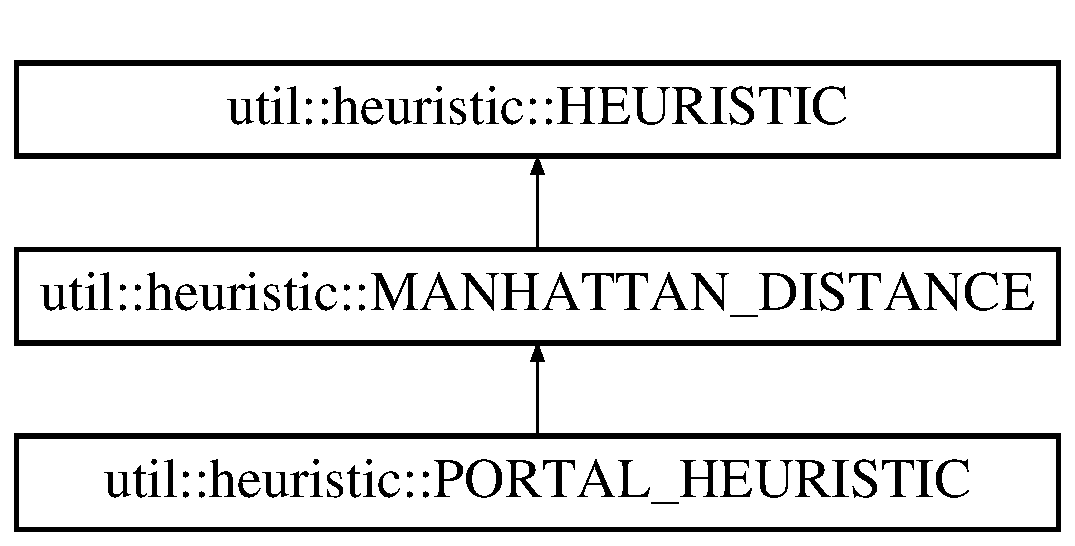
\includegraphics[height=3.000000cm]{structutil_1_1heuristic_1_1_p_o_r_t_a_l___h_e_u_r_i_s_t_i_c}
\end{center}
\end{figure}
\subsection*{Public Member Functions}
\begin{DoxyCompactItemize}
\item 
{\bfseries P\+O\+R\+T\+A\+L\+\_\+\+H\+E\+U\+R\+I\+S\+T\+IC} (\hyperlink{class_entity_system}{Entity\+System} \&ents)\hypertarget{structutil_1_1heuristic_1_1_p_o_r_t_a_l___h_e_u_r_i_s_t_i_c_a845d5561ba3d903c2518b28300e2ba49}{}\label{structutil_1_1heuristic_1_1_p_o_r_t_a_l___h_e_u_r_i_s_t_i_c_a845d5561ba3d903c2518b28300e2ba49}

\item 
tdt\+::real {\bfseries get\+\_\+cost} (tdt\+::uint id1, tdt\+::uint id2) override\hypertarget{structutil_1_1heuristic_1_1_p_o_r_t_a_l___h_e_u_r_i_s_t_i_c_a63bd677b75d03ac3d26b47e56eaf7ce6}{}\label{structutil_1_1heuristic_1_1_p_o_r_t_a_l___h_e_u_r_i_s_t_i_c_a63bd677b75d03ac3d26b47e56eaf7ce6}

\end{DoxyCompactItemize}
\subsection*{Private Member Functions}
\begin{DoxyCompactItemize}
\item 
std\+::tuple$<$ tdt\+::uint, tdt\+::uint $>$ \hyperlink{structutil_1_1heuristic_1_1_p_o_r_t_a_l___h_e_u_r_i_s_t_i_c_ab49ded73b51452534aaea1383a44b9db}{get\+\_\+closest\+\_\+portal} (tdt\+::uint id)
\begin{DoxyCompactList}\small\item\em Returns the nodes that have the closest portal pair from a given entity on them. \end{DoxyCompactList}\end{DoxyCompactItemize}
\subsection*{Additional Inherited Members}


\subsection{Detailed Description}
Variation of the Manhattan distance heuristic that takes portals into accounts. 

\begin{DoxyNote}{Note}
This heuristic won\textquotesingle{}t help with complex chains of portals. For that, the B\+E\+S\+T\+\_\+\+P\+A\+TH path type would be needed to check every single portal combination. (But for basic portal usage, this heuristic works fine.) 
\end{DoxyNote}


Definition at line 267 of file Pathfinding\+Algorithms.\+hpp.



\subsection{Member Function Documentation}
\index{util\+::heuristic\+::\+P\+O\+R\+T\+A\+L\+\_\+\+H\+E\+U\+R\+I\+S\+T\+IC@{util\+::heuristic\+::\+P\+O\+R\+T\+A\+L\+\_\+\+H\+E\+U\+R\+I\+S\+T\+IC}!get\+\_\+closest\+\_\+portal@{get\+\_\+closest\+\_\+portal}}
\index{get\+\_\+closest\+\_\+portal@{get\+\_\+closest\+\_\+portal}!util\+::heuristic\+::\+P\+O\+R\+T\+A\+L\+\_\+\+H\+E\+U\+R\+I\+S\+T\+IC@{util\+::heuristic\+::\+P\+O\+R\+T\+A\+L\+\_\+\+H\+E\+U\+R\+I\+S\+T\+IC}}
\subsubsection[{\texorpdfstring{get\+\_\+closest\+\_\+portal(tdt\+::uint id)}{get_closest_portal(tdt::uint id)}}]{\setlength{\rightskip}{0pt plus 5cm}std\+::tuple$<$tdt\+::uint, tdt\+::uint$>$ util\+::heuristic\+::\+P\+O\+R\+T\+A\+L\+\_\+\+H\+E\+U\+R\+I\+S\+T\+I\+C\+::get\+\_\+closest\+\_\+portal (
\begin{DoxyParamCaption}
\item[{tdt\+::uint}]{id}
\end{DoxyParamCaption}
)\hspace{0.3cm}{\ttfamily [inline]}, {\ttfamily [private]}}\hypertarget{structutil_1_1heuristic_1_1_p_o_r_t_a_l___h_e_u_r_i_s_t_i_c_ab49ded73b51452534aaea1383a44b9db}{}\label{structutil_1_1heuristic_1_1_p_o_r_t_a_l___h_e_u_r_i_s_t_i_c_ab49ded73b51452534aaea1383a44b9db}


Returns the nodes that have the closest portal pair from a given entity on them. 


\begin{DoxyParams}{Parameters}
{\em ID} & of the entity. \\
\hline
\end{DoxyParams}


Definition at line 298 of file Pathfinding\+Algorithms.\+hpp.



The documentation for this struct was generated from the following file\+:\begin{DoxyCompactItemize}
\item 
tools/Pathfinding\+Algorithms.\+hpp\end{DoxyCompactItemize}

\hypertarget{struct_portal_component}{}\section{Portal\+Component Struct Reference}
\label{struct_portal_component}\index{Portal\+Component@{Portal\+Component}}


Dummy component that signals that an entity having it is a portal -\/ which is used in pathfinding.  




{\ttfamily \#include $<$Components.\+hpp$>$}

\subsection*{Static Public Attributes}
\begin{DoxyCompactItemize}
\item 
static constexpr int {\bfseries type} = 39\hypertarget{struct_portal_component_afdcd2a4887aef400c454143f1c384e7d}{}\label{struct_portal_component_afdcd2a4887aef400c454143f1c384e7d}

\end{DoxyCompactItemize}


\subsection{Detailed Description}
Dummy component that signals that an entity having it is a portal -\/ which is used in pathfinding. 

Definition at line 899 of file Components.\+hpp.



The documentation for this struct was generated from the following file\+:\begin{DoxyCompactItemize}
\item 
Components.\+hpp\end{DoxyCompactItemize}

\hypertarget{struct_price_component}{}\section{Price\+Component Struct Reference}
\label{struct_price_component}\index{Price\+Component@{Price\+Component}}


Represents either gold or mana cost of an entity.  




{\ttfamily \#include $<$Components.\+hpp$>$}

\subsection*{Public Member Functions}
\begin{DoxyCompactItemize}
\item 
{\bfseries Price\+Component} (tdt\+::uint p=0)\hypertarget{struct_price_component_a46bf31ddd3c5eb3570a14a8f0d9d64eb}{}\label{struct_price_component_a46bf31ddd3c5eb3570a14a8f0d9d64eb}

\item 
{\bfseries Price\+Component} (const \hyperlink{struct_price_component}{Price\+Component} \&)=default\hypertarget{struct_price_component_a2c5d8e7a536cd3549cce05553af77f42}{}\label{struct_price_component_a2c5d8e7a536cd3549cce05553af77f42}

\item 
{\bfseries Price\+Component} (\hyperlink{struct_price_component}{Price\+Component} \&\&)=default\hypertarget{struct_price_component_a6d90e1366e588476e431fc97c214c493}{}\label{struct_price_component_a6d90e1366e588476e431fc97c214c493}

\item 
\hyperlink{struct_price_component}{Price\+Component} \& {\bfseries operator=} (const \hyperlink{struct_price_component}{Price\+Component} \&)=default\hypertarget{struct_price_component_a068427317c564a177fe20089f85c26e0}{}\label{struct_price_component_a068427317c564a177fe20089f85c26e0}

\item 
\hyperlink{struct_price_component}{Price\+Component} \& {\bfseries operator=} (\hyperlink{struct_price_component}{Price\+Component} \&\&)=default\hypertarget{struct_price_component_a5b0a8b4a512c21bef557da7640d5ca77}{}\label{struct_price_component_a5b0a8b4a512c21bef557da7640d5ca77}

\end{DoxyCompactItemize}
\subsection*{Public Attributes}
\begin{DoxyCompactItemize}
\item 
tdt\+::uint {\bfseries price}\hypertarget{struct_price_component_a05bed34eebceb5eb22a36ee130bf7c3b}{}\label{struct_price_component_a05bed34eebceb5eb22a36ee130bf7c3b}

\end{DoxyCompactItemize}
\subsection*{Static Public Attributes}
\begin{DoxyCompactItemize}
\item 
static constexpr int {\bfseries type} = 23\hypertarget{struct_price_component_aa93ef46a1b17086f36590ec57f0e6c76}{}\label{struct_price_component_aa93ef46a1b17086f36590ec57f0e6c76}

\end{DoxyCompactItemize}


\subsection{Detailed Description}
Represents either gold or mana cost of an entity. 

Definition at line 568 of file Components.\+hpp.



The documentation for this struct was generated from the following file\+:\begin{DoxyCompactItemize}
\item 
Components.\+hpp\end{DoxyCompactItemize}

\hypertarget{struct_product_component}{}\section{Product\+Component Struct Reference}
\label{struct_product_component}\index{Product\+Component@{Product\+Component}}


References the producer of the entity that has this component.  




{\ttfamily \#include $<$Components.\+hpp$>$}

\subsection*{Public Member Functions}
\begin{DoxyCompactItemize}
\item 
{\bfseries Product\+Component} (tdt\+::uint prod\+\_\+id=Component\+::\+N\+O\+\_\+\+E\+N\+T\+I\+TY)\hypertarget{struct_product_component_ab40e40098680fa386f66bae4c175fbfb}{}\label{struct_product_component_ab40e40098680fa386f66bae4c175fbfb}

\item 
{\bfseries Product\+Component} (const \hyperlink{struct_product_component}{Product\+Component} \&)=default\hypertarget{struct_product_component_afd6dffca5d8adeff03db3f2cea9c24ee}{}\label{struct_product_component_afd6dffca5d8adeff03db3f2cea9c24ee}

\item 
{\bfseries Product\+Component} (\hyperlink{struct_product_component}{Product\+Component} \&\&)=default\hypertarget{struct_product_component_a56da8b4c79e4cd859ccc666955f0dcbc}{}\label{struct_product_component_a56da8b4c79e4cd859ccc666955f0dcbc}

\item 
\hyperlink{struct_product_component}{Product\+Component} \& {\bfseries operator=} (const \hyperlink{struct_product_component}{Product\+Component} \&)=default\hypertarget{struct_product_component_a9d1580b127ad15f2a65d8e96d1b533c1}{}\label{struct_product_component_a9d1580b127ad15f2a65d8e96d1b533c1}

\item 
\hyperlink{struct_product_component}{Product\+Component} \& {\bfseries operator=} (\hyperlink{struct_product_component}{Product\+Component} \&\&)=default\hypertarget{struct_product_component_a23c4ad5316f90f831a15ec2a088c8cb3}{}\label{struct_product_component_a23c4ad5316f90f831a15ec2a088c8cb3}

\end{DoxyCompactItemize}
\subsection*{Public Attributes}
\begin{DoxyCompactItemize}
\item 
tdt\+::uint {\bfseries producer}\hypertarget{struct_product_component_a7e27a73608ff0670c2774909fc573e18}{}\label{struct_product_component_a7e27a73608ff0670c2774909fc573e18}

\end{DoxyCompactItemize}
\subsection*{Static Public Attributes}
\begin{DoxyCompactItemize}
\item 
static constexpr int {\bfseries type} = 13\hypertarget{struct_product_component_a9a7ca437ccf7aee4e6a624f214e12320}{}\label{struct_product_component_a9a7ca437ccf7aee4e6a624f214e12320}

\end{DoxyCompactItemize}


\subsection{Detailed Description}
References the producer of the entity that has this component. 

(Producer == building/tile that spawned it.) 

Definition at line 348 of file Components.\+hpp.



The documentation for this struct was generated from the following file\+:\begin{DoxyCompactItemize}
\item 
Components.\+hpp\end{DoxyCompactItemize}

\hypertarget{struct_production_component}{}\section{Production\+Component Struct Reference}
\label{struct_production_component}\index{Production\+Component@{Production\+Component}}


Allows scheduled production of new entities (spawners) of a given type up to a maximum amount.  




{\ttfamily \#include $<$Components.\+hpp$>$}

\subsection*{Public Member Functions}
\begin{DoxyCompactItemize}
\item 
{\bfseries Production\+Component} (std\+::string \&\&b=\char`\"{}E\+R\+R\+OR\char`\"{}, tdt\+::uint l=1, tdt\+::real cd=0.f)\hypertarget{struct_production_component_ac016ba62c862a7e0afed63bbc5980614}{}\label{struct_production_component_ac016ba62c862a7e0afed63bbc5980614}

\item 
{\bfseries Production\+Component} (const \hyperlink{struct_production_component}{Production\+Component} \&)=default\hypertarget{struct_production_component_ae7f2dc96fcc114cfa1c8315baa4943b3}{}\label{struct_production_component_ae7f2dc96fcc114cfa1c8315baa4943b3}

\item 
{\bfseries Production\+Component} (\hyperlink{struct_production_component}{Production\+Component} \&\&)=default\hypertarget{struct_production_component_abb4436011d2a4bd61d9a0671b33987d1}{}\label{struct_production_component_abb4436011d2a4bd61d9a0671b33987d1}

\item 
\hyperlink{struct_production_component}{Production\+Component} \& {\bfseries operator=} (const \hyperlink{struct_production_component}{Production\+Component} \&)=default\hypertarget{struct_production_component_a6568dff88a6c69b22b581e7eb7400a4f}{}\label{struct_production_component_a6568dff88a6c69b22b581e7eb7400a4f}

\item 
\hyperlink{struct_production_component}{Production\+Component} \& {\bfseries operator=} (\hyperlink{struct_production_component}{Production\+Component} \&\&)=default\hypertarget{struct_production_component_ae06df6fe33cead3950ea5e641f38199b}{}\label{struct_production_component_ae06df6fe33cead3950ea5e641f38199b}

\end{DoxyCompactItemize}
\subsection*{Public Attributes}
\begin{DoxyCompactItemize}
\item 
std\+::string {\bfseries product\+\_\+blueprint}\hypertarget{struct_production_component_ae0880bbbc20032b4d1182630190d7b62}{}\label{struct_production_component_ae0880bbbc20032b4d1182630190d7b62}

\item 
tdt\+::uint {\bfseries curr\+\_\+produced}\hypertarget{struct_production_component_adaf8a9fa51936b32a352314fa2e524ad}{}\label{struct_production_component_adaf8a9fa51936b32a352314fa2e524ad}

\item 
tdt\+::uint {\bfseries max\+\_\+produced}\hypertarget{struct_production_component_a96d04bf54602b9efcc891ad22cdae1be}{}\label{struct_production_component_a96d04bf54602b9efcc891ad22cdae1be}

\item 
tdt\+::real {\bfseries cooldown}\hypertarget{struct_production_component_ae2e97e438f56b14a3db1f27257d65373}{}\label{struct_production_component_ae2e97e438f56b14a3db1f27257d65373}

\item 
tdt\+::real {\bfseries curr\+\_\+cd}\hypertarget{struct_production_component_af27b0ff0455756914c1f82133d8ca14c}{}\label{struct_production_component_af27b0ff0455756914c1f82133d8ca14c}

\end{DoxyCompactItemize}
\subsection*{Static Public Attributes}
\begin{DoxyCompactItemize}
\item 
static constexpr int {\bfseries type} = 11\hypertarget{struct_production_component_a318238033df2b0daf7a43e777760c6fb}{}\label{struct_production_component_a318238033df2b0daf7a43e777760c6fb}

\end{DoxyCompactItemize}


\subsection{Detailed Description}
Allows scheduled production of new entities (spawners) of a given type up to a maximum amount. 

Definition at line 294 of file Components.\+hpp.



The documentation for this struct was generated from the following file\+:\begin{DoxyCompactItemize}
\item 
Components.\+hpp\end{DoxyCompactItemize}

\hypertarget{class_production_system}{}\section{Production\+System Class Reference}
\label{class_production_system}\index{Production\+System@{Production\+System}}


\hyperlink{class_system}{System} taking care of entities spawned by buildings and the spawn counts allowing for a constant amount of entities (related to the number of buildings spawning entities of that blueprint table).  




{\ttfamily \#include $<$Production\+System.\+hpp$>$}

Inheritance diagram for Production\+System\+:\begin{figure}[H]
\begin{center}
\leavevmode
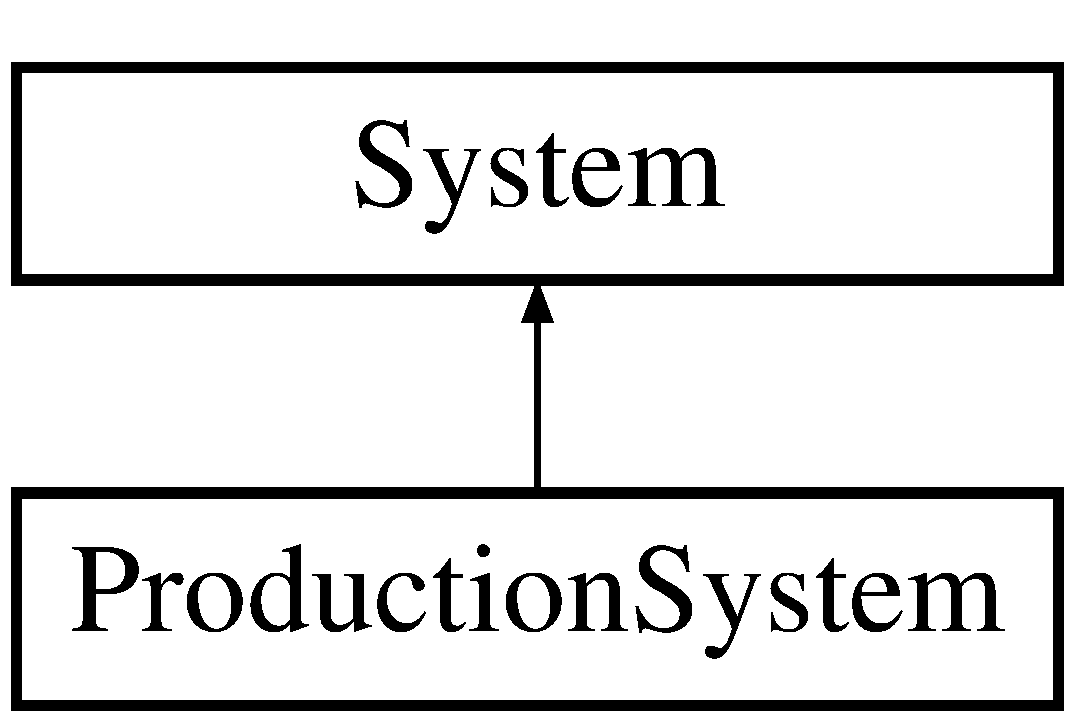
\includegraphics[height=2.000000cm]{class_production_system}
\end{center}
\end{figure}
\subsection*{Public Member Functions}
\begin{DoxyCompactItemize}
\item 
\hyperlink{class_production_system_a0714612f29ebaca91f6cd750062f4090}{Production\+System} (\hyperlink{class_entity_system}{Entity\+System} \&)
\begin{DoxyCompactList}\small\item\em Constructor. \end{DoxyCompactList}\item 
\hyperlink{class_production_system_a65622ad0ab7cb6e3ea0b260697ab5928}{$\sim$\+Production\+System} ()
\begin{DoxyCompactList}\small\item\em Destructor. \end{DoxyCompactList}\item 
void \hyperlink{class_production_system_ad8d47ea05eeb8504a58c2f68f9285c35}{update} (tdt\+::real) override
\begin{DoxyCompactList}\small\item\em Iterates over all buildings and when possible, spawns new entities. \end{DoxyCompactList}\item 
void \hyperlink{class_production_system_a285816be3e143ec79a330e7af5ad3eca}{spawn\+\_\+entity} (tdt\+::uint, const std\+::string \&)
\begin{DoxyCompactList}\small\item\em Spawns a single entity created by a building. \end{DoxyCompactList}\item 
void \hyperlink{class_production_system_a189615e653da1dc7773efe1ca2c98863}{set\+\_\+time\+\_\+multiplier} (tdt\+::real)
\begin{DoxyCompactList}\small\item\em Sets the time value by which the frame times are multiplied when added to the production timers. \end{DoxyCompactList}\item 
tdt\+::real \hyperlink{class_production_system_abf59007923dc29a23db218200e0b75d9}{get\+\_\+time\+\_\+multiplier} ()
\begin{DoxyCompactList}\small\item\em Returns the time value by which the frame times are multiplied when added to the production timers. \end{DoxyCompactList}\end{DoxyCompactItemize}
\subsection*{Private Attributes}
\begin{DoxyCompactItemize}
\item 
\hyperlink{class_entity_system}{Entity\+System} \& \hyperlink{class_production_system_a1635990974ff715fd1ac2035f9760e51}{entities\+\_\+}
\begin{DoxyCompactList}\small\item\em Reference to the game\textquotesingle{}s entity system (component retrieval). \end{DoxyCompactList}\item 
\hyperlink{class_grid}{Grid} \& \hyperlink{class_production_system_a7b57e417c67f4629e5b858b3f55edbf4}{grid\+\_\+}
\begin{DoxyCompactList}\small\item\em Reference to the game\textquotesingle{}s pathfinding grid (spawn positioning). \end{DoxyCompactList}\item 
tdt\+::real \hyperlink{class_production_system_a0d1e37301b0549aa967c561c6f8f876e}{time\+\_\+multiplier\+\_\+}
\begin{DoxyCompactList}\small\item\em Allows to speed up/slow down the production of all buildings. \end{DoxyCompactList}\end{DoxyCompactItemize}


\subsection{Detailed Description}
\hyperlink{class_system}{System} taking care of entities spawned by buildings and the spawn counts allowing for a constant amount of entities (related to the number of buildings spawning entities of that blueprint table). 

Definition at line 14 of file Production\+System.\+hpp.



\subsection{Constructor \& Destructor Documentation}
\index{Production\+System@{Production\+System}!Production\+System@{Production\+System}}
\index{Production\+System@{Production\+System}!Production\+System@{Production\+System}}
\subsubsection[{\texorpdfstring{Production\+System(\+Entity\+System \&)}{ProductionSystem(EntitySystem &)}}]{\setlength{\rightskip}{0pt plus 5cm}Production\+System\+::\+Production\+System (
\begin{DoxyParamCaption}
\item[{{\bf Entity\+System} \&}]{ents}
\end{DoxyParamCaption}
)}\hypertarget{class_production_system_a0714612f29ebaca91f6cd750062f4090}{}\label{class_production_system_a0714612f29ebaca91f6cd750062f4090}


Constructor. 


\begin{DoxyParams}{Parameters}
{\em Reference} & to the game\textquotesingle{}s entity system. \\
\hline
\end{DoxyParams}


Definition at line 7 of file Production\+System.\+cpp.

\index{Production\+System@{Production\+System}!````~Production\+System@{$\sim$\+Production\+System}}
\index{````~Production\+System@{$\sim$\+Production\+System}!Production\+System@{Production\+System}}
\subsubsection[{\texorpdfstring{$\sim$\+Production\+System()}{~ProductionSystem()}}]{\setlength{\rightskip}{0pt plus 5cm}Production\+System\+::$\sim$\+Production\+System (
\begin{DoxyParamCaption}
{}
\end{DoxyParamCaption}
)\hspace{0.3cm}{\ttfamily [inline]}}\hypertarget{class_production_system_a65622ad0ab7cb6e3ea0b260697ab5928}{}\label{class_production_system_a65622ad0ab7cb6e3ea0b260697ab5928}


Destructor. 



Definition at line 26 of file Production\+System.\+hpp.



\subsection{Member Function Documentation}
\index{Production\+System@{Production\+System}!get\+\_\+time\+\_\+multiplier@{get\+\_\+time\+\_\+multiplier}}
\index{get\+\_\+time\+\_\+multiplier@{get\+\_\+time\+\_\+multiplier}!Production\+System@{Production\+System}}
\subsubsection[{\texorpdfstring{get\+\_\+time\+\_\+multiplier()}{get_time_multiplier()}}]{\setlength{\rightskip}{0pt plus 5cm}tdt\+::real Production\+System\+::get\+\_\+time\+\_\+multiplier (
\begin{DoxyParamCaption}
{}
\end{DoxyParamCaption}
)}\hypertarget{class_production_system_abf59007923dc29a23db218200e0b75d9}{}\label{class_production_system_abf59007923dc29a23db218200e0b75d9}


Returns the time value by which the frame times are multiplied when added to the production timers. 



Definition at line 125 of file Production\+System.\+cpp.

\index{Production\+System@{Production\+System}!set\+\_\+time\+\_\+multiplier@{set\+\_\+time\+\_\+multiplier}}
\index{set\+\_\+time\+\_\+multiplier@{set\+\_\+time\+\_\+multiplier}!Production\+System@{Production\+System}}
\subsubsection[{\texorpdfstring{set\+\_\+time\+\_\+multiplier(tdt\+::real)}{set_time_multiplier(tdt::real)}}]{\setlength{\rightskip}{0pt plus 5cm}void Production\+System\+::set\+\_\+time\+\_\+multiplier (
\begin{DoxyParamCaption}
\item[{tdt\+::real}]{val}
\end{DoxyParamCaption}
)}\hypertarget{class_production_system_a189615e653da1dc7773efe1ca2c98863}{}\label{class_production_system_a189615e653da1dc7773efe1ca2c98863}


Sets the time value by which the frame times are multiplied when added to the production timers. 


\begin{DoxyParams}{Parameters}
{\em The} & new time multiplier. \\
\hline
\end{DoxyParams}


Definition at line 120 of file Production\+System.\+cpp.

\index{Production\+System@{Production\+System}!spawn\+\_\+entity@{spawn\+\_\+entity}}
\index{spawn\+\_\+entity@{spawn\+\_\+entity}!Production\+System@{Production\+System}}
\subsubsection[{\texorpdfstring{spawn\+\_\+entity(tdt\+::uint, const std\+::string \&)}{spawn_entity(tdt::uint, const std::string &)}}]{\setlength{\rightskip}{0pt plus 5cm}void Production\+System\+::spawn\+\_\+entity (
\begin{DoxyParamCaption}
\item[{tdt\+::uint}]{producer, }
\item[{const std\+::string \&}]{blueprint}
\end{DoxyParamCaption}
)}\hypertarget{class_production_system_a285816be3e143ec79a330e7af5ad3eca}{}\label{class_production_system_a285816be3e143ec79a330e7af5ad3eca}


Spawns a single entity created by a building. 


\begin{DoxyParams}{Parameters}
{\em ID} & of the building. \\
\hline
{\em Name} & of the blueprint table of the spawned entity. \\
\hline
\end{DoxyParams}
This checks all edges of the building to find a free spot for the entity to spawn on.

Definition at line 29 of file Production\+System.\+cpp.

\index{Production\+System@{Production\+System}!update@{update}}
\index{update@{update}!Production\+System@{Production\+System}}
\subsubsection[{\texorpdfstring{update(tdt\+::real) override}{update(tdt::real) override}}]{\setlength{\rightskip}{0pt plus 5cm}void Production\+System\+::update (
\begin{DoxyParamCaption}
\item[{tdt\+::real}]{delta}
\end{DoxyParamCaption}
)\hspace{0.3cm}{\ttfamily [override]}, {\ttfamily [virtual]}}\hypertarget{class_production_system_ad8d47ea05eeb8504a58c2f68f9285c35}{}\label{class_production_system_ad8d47ea05eeb8504a58c2f68f9285c35}


Iterates over all buildings and when possible, spawns new entities. 


\begin{DoxyParams}{Parameters}
{\em Time} & since last frame. \\
\hline
\end{DoxyParams}


Implements \hyperlink{class_system_a6d54c9bd38eb43d620a1451cb0925472}{System}.



Definition at line 11 of file Production\+System.\+cpp.



\subsection{Member Data Documentation}
\index{Production\+System@{Production\+System}!entities\+\_\+@{entities\+\_\+}}
\index{entities\+\_\+@{entities\+\_\+}!Production\+System@{Production\+System}}
\subsubsection[{\texorpdfstring{entities\+\_\+}{entities_}}]{\setlength{\rightskip}{0pt plus 5cm}{\bf Entity\+System}\& Production\+System\+::entities\+\_\+\hspace{0.3cm}{\ttfamily [private]}}\hypertarget{class_production_system_a1635990974ff715fd1ac2035f9760e51}{}\label{class_production_system_a1635990974ff715fd1ac2035f9760e51}


Reference to the game\textquotesingle{}s entity system (component retrieval). 



Definition at line 58 of file Production\+System.\+hpp.

\index{Production\+System@{Production\+System}!grid\+\_\+@{grid\+\_\+}}
\index{grid\+\_\+@{grid\+\_\+}!Production\+System@{Production\+System}}
\subsubsection[{\texorpdfstring{grid\+\_\+}{grid_}}]{\setlength{\rightskip}{0pt plus 5cm}{\bf Grid}\& Production\+System\+::grid\+\_\+\hspace{0.3cm}{\ttfamily [private]}}\hypertarget{class_production_system_a7b57e417c67f4629e5b858b3f55edbf4}{}\label{class_production_system_a7b57e417c67f4629e5b858b3f55edbf4}


Reference to the game\textquotesingle{}s pathfinding grid (spawn positioning). 



Definition at line 63 of file Production\+System.\+hpp.

\index{Production\+System@{Production\+System}!time\+\_\+multiplier\+\_\+@{time\+\_\+multiplier\+\_\+}}
\index{time\+\_\+multiplier\+\_\+@{time\+\_\+multiplier\+\_\+}!Production\+System@{Production\+System}}
\subsubsection[{\texorpdfstring{time\+\_\+multiplier\+\_\+}{time_multiplier_}}]{\setlength{\rightskip}{0pt plus 5cm}tdt\+::real Production\+System\+::time\+\_\+multiplier\+\_\+\hspace{0.3cm}{\ttfamily [private]}}\hypertarget{class_production_system_a0d1e37301b0549aa967c561c6f8f876e}{}\label{class_production_system_a0d1e37301b0549aa967c561c6f8f876e}


Allows to speed up/slow down the production of all buildings. 



Definition at line 68 of file Production\+System.\+hpp.



The documentation for this class was generated from the following files\+:\begin{DoxyCompactItemize}
\item 
systems/Production\+System.\+hpp\item 
systems/Production\+System.\+cpp\end{DoxyCompactItemize}

\hypertarget{structutil_1_1path__type_1_1_r_a_n_d_o_m___p_a_t_h}{}\section{util\+:\+:path\+\_\+type\+:\+:R\+A\+N\+D\+O\+M\+\_\+\+P\+A\+TH$<$ U\+P\+P\+ER $>$ Struct Template Reference}
\label{structutil_1_1path__type_1_1_r_a_n_d_o_m___p_a_t_h}\index{util\+::path\+\_\+type\+::\+R\+A\+N\+D\+O\+M\+\_\+\+P\+A\+T\+H$<$ U\+P\+P\+E\+R $>$@{util\+::path\+\_\+type\+::\+R\+A\+N\+D\+O\+M\+\_\+\+P\+A\+T\+H$<$ U\+P\+P\+E\+R $>$}}


Finds a random path by returning true only when a random number in the range (0, U\+P\+P\+ER) is equal to 0.  




{\ttfamily \#include $<$Pathfinding\+Algorithms.\+hpp$>$}

\subsection*{Static Public Member Functions}
\begin{DoxyCompactItemize}
\item 
static bool {\bfseries return\+\_\+path} ()\hypertarget{structutil_1_1path__type_1_1_r_a_n_d_o_m___p_a_t_h_a0bd9f0114254e938fd4b9a0f63ddb59f}{}\label{structutil_1_1path__type_1_1_r_a_n_d_o_m___p_a_t_h_a0bd9f0114254e938fd4b9a0f63ddb59f}

\end{DoxyCompactItemize}


\subsection{Detailed Description}
\subsubsection*{template$<$int U\+P\+P\+ER$>$\\*
struct util\+::path\+\_\+type\+::\+R\+A\+N\+D\+O\+M\+\_\+\+P\+A\+T\+H$<$ U\+P\+P\+E\+R $>$}

Finds a random path by returning true only when a random number in the range (0, U\+P\+P\+ER) is equal to 0. 

(U\+P\+P\+ER is specialized as a template parameter.) 

Definition at line 169 of file Pathfinding\+Algorithms.\+hpp.



The documentation for this struct was generated from the following file\+:\begin{DoxyCompactItemize}
\item 
tools/Pathfinding\+Algorithms.\+hpp\end{DoxyCompactItemize}

\hypertarget{classlevel__generators_1_1_random_level_generator}{}\section{level\+\_\+generators\+:\+:Random\+Level\+Generator Class Reference}
\label{classlevel__generators_1_1_random_level_generator}\index{level\+\_\+generators\+::\+Random\+Level\+Generator@{level\+\_\+generators\+::\+Random\+Level\+Generator}}


Level generator that uses simple R\+NG approach (counts the number of gold neighbours and increases the chance to spawn a gold deposit if needed).  




{\ttfamily \#include $<$Level\+Generators.\+hpp$>$}

Inheritance diagram for level\+\_\+generators\+:\+:Random\+Level\+Generator\+:\begin{figure}[H]
\begin{center}
\leavevmode
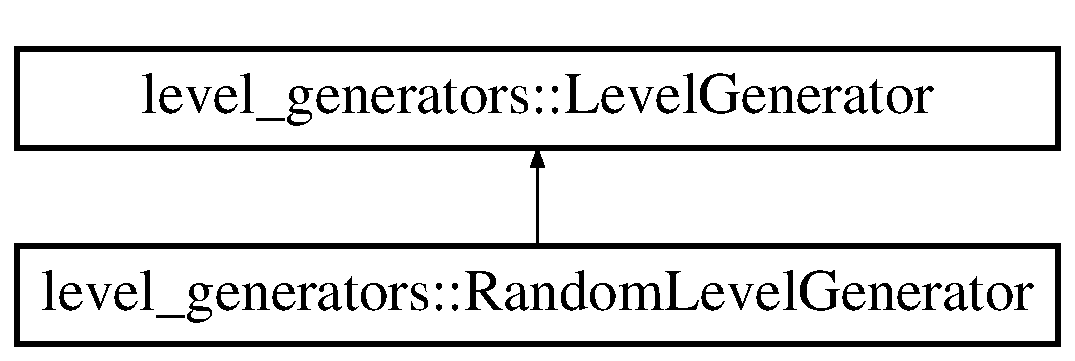
\includegraphics[height=2.000000cm]{classlevel__generators_1_1_random_level_generator}
\end{center}
\end{figure}
\subsection*{Public Member Functions}
\begin{DoxyCompactItemize}
\item 
\hyperlink{classlevel__generators_1_1_random_level_generator_ae599a19573e7ac5ffb0c4834754df933}{Random\+Level\+Generator} (\hyperlink{class_entity_system}{Entity\+System} \&, tdt\+::uint)
\begin{DoxyCompactList}\small\item\em Constructor. \end{DoxyCompactList}\item 
void \hyperlink{classlevel__generators_1_1_random_level_generator_a085098cd10565bd3f9c6b13f68fcc1cb}{generate} (tdt\+::uint, tdt\+::uint, \hyperlink{class_wave_system}{Wave\+System} \&) override
\begin{DoxyCompactList}\small\item\em Generates a level with the given dimensions using an R\+NG approach. \end{DoxyCompactList}\end{DoxyCompactItemize}
\subsection*{Additional Inherited Members}


\subsection{Detailed Description}
Level generator that uses simple R\+NG approach (counts the number of gold neighbours and increases the chance to spawn a gold deposit if needed). 

Definition at line 60 of file Level\+Generators.\+hpp.



\subsection{Constructor \& Destructor Documentation}
\index{level\+\_\+generators\+::\+Random\+Level\+Generator@{level\+\_\+generators\+::\+Random\+Level\+Generator}!Random\+Level\+Generator@{Random\+Level\+Generator}}
\index{Random\+Level\+Generator@{Random\+Level\+Generator}!level\+\_\+generators\+::\+Random\+Level\+Generator@{level\+\_\+generators\+::\+Random\+Level\+Generator}}
\subsubsection[{\texorpdfstring{Random\+Level\+Generator(\+Entity\+System \&, tdt\+::uint)}{RandomLevelGenerator(EntitySystem &, tdt::uint)}}]{\setlength{\rightskip}{0pt plus 5cm}level\+\_\+generators\+::\+Random\+Level\+Generator\+::\+Random\+Level\+Generator (
\begin{DoxyParamCaption}
\item[{{\bf Entity\+System} \&}]{ents, }
\item[{tdt\+::uint}]{c}
\end{DoxyParamCaption}
)}\hypertarget{classlevel__generators_1_1_random_level_generator_ae599a19573e7ac5ffb0c4834754df933}{}\label{classlevel__generators_1_1_random_level_generator_ae599a19573e7ac5ffb0c4834754df933}


Constructor. 


\begin{DoxyParams}{Parameters}
{\em Entity} & system that contains the level\textquotesingle{}s entities. \\
\hline
{\em Number} & of iterations done while generating. \\
\hline
\end{DoxyParams}


Definition at line 14 of file Level\+Generators.\+cpp.



\subsection{Member Function Documentation}
\index{level\+\_\+generators\+::\+Random\+Level\+Generator@{level\+\_\+generators\+::\+Random\+Level\+Generator}!generate@{generate}}
\index{generate@{generate}!level\+\_\+generators\+::\+Random\+Level\+Generator@{level\+\_\+generators\+::\+Random\+Level\+Generator}}
\subsubsection[{\texorpdfstring{generate(tdt\+::uint, tdt\+::uint, Wave\+System \&) override}{generate(tdt::uint, tdt::uint, WaveSystem &) override}}]{\setlength{\rightskip}{0pt plus 5cm}void level\+\_\+generators\+::\+Random\+Level\+Generator\+::generate (
\begin{DoxyParamCaption}
\item[{tdt\+::uint}]{width, }
\item[{tdt\+::uint}]{height, }
\item[{{\bf Wave\+System} \&}]{wsystem}
\end{DoxyParamCaption}
)\hspace{0.3cm}{\ttfamily [override]}, {\ttfamily [virtual]}}\hypertarget{classlevel__generators_1_1_random_level_generator_a085098cd10565bd3f9c6b13f68fcc1cb}{}\label{classlevel__generators_1_1_random_level_generator_a085098cd10565bd3f9c6b13f68fcc1cb}


Generates a level with the given dimensions using an R\+NG approach. 


\begin{DoxyParams}{Parameters}
{\em Width} & of the level. \\
\hline
{\em Height} & of the level. \\
\hline
{\em Wave} & system that will have it\textquotesingle{}s spawn nodes set. \\
\hline
\end{DoxyParams}
0 == free space 1 == wall 2 == gold deposit 3 == border 4 == walkway 5 == light source 6 == throne 7 == vault 8 == mine

Implements \hyperlink{classlevel__generators_1_1_level_generator_af5c177ea2e5b14b983c47c8c169c5ac7}{level\+\_\+generators\+::\+Level\+Generator}.



Definition at line 18 of file Level\+Generators.\+cpp.



The documentation for this class was generated from the following files\+:\begin{DoxyCompactItemize}
\item 
tools/Level\+Generators.\+hpp\item 
tools/Level\+Generators.\+cpp\end{DoxyCompactItemize}

\hypertarget{class_ray_caster}{}\section{Ray\+Caster Class Reference}
\label{class_ray_caster}\index{Ray\+Caster@{Ray\+Caster}}


Manages polygon precise raycasting used with half walls that have empty spaces in their bounding boxes.  




{\ttfamily \#include $<$Ray\+Caster.\+hpp$>$}

\subsection*{Public Member Functions}
\begin{DoxyCompactItemize}
\item 
\hyperlink{class_ray_caster_a216827ccaf7a65fc6e25953fe015d9bc}{Ray\+Caster} (Ogre\+::\+Scene\+Manager \&)
\begin{DoxyCompactList}\small\item\em Constructor. \end{DoxyCompactList}\item 
std\+::pair$<$ bool, tdt\+::real $>$ \hyperlink{class_ray_caster_a5af376ca167daa1e997a73f96bdbcbde}{cast} (const Ogre\+::\+Vector3 \&, const Ogre\+::\+Vector3 \&, const std\+::string \&=\char`\"{}\char`\"{}) const 
\begin{DoxyCompactList}\small\item\em Casts a ray that checks for polygon level collisions on it\textquotesingle{}s way. \end{DoxyCompactList}\end{DoxyCompactItemize}
\subsection*{Private Member Functions}
\begin{DoxyCompactItemize}
\item 
void \hyperlink{class_ray_caster_a6c098462b63c0cdac3cc1a3ea4609bfb}{get\+\_\+info} (const Ogre\+::\+Entity \&, tdt\+::uint \&, tdt\+::uint \&, std\+::vector$<$ Ogre\+::\+Vector3 $>$ \&, std\+::vector$<$ tdt\+::uint $>$ \&, const Ogre\+::\+Vector3 \&, const Ogre\+::\+Quaternion \&, const Ogre\+::\+Vector3 \&) const 
\begin{DoxyCompactList}\small\item\em Returns information about vertices of an entity by modifying it\textquotesingle{}s size\+\_\+t and vector parameters. \end{DoxyCompactList}\end{DoxyCompactItemize}
\subsection*{Private Attributes}
\begin{DoxyCompactItemize}
\item 
Ogre\+::\+Ray\+Scene\+Query $\ast$ \hyperlink{class_ray_caster_ab086a0e4d34aa835c2a5289ee786832e}{query\+\_\+}
\begin{DoxyCompactList}\small\item\em Query used for the collision ray cast. \end{DoxyCompactList}\end{DoxyCompactItemize}


\subsection{Detailed Description}
Manages polygon precise raycasting used with half walls that have empty spaces in their bounding boxes. 

\begin{DoxyNote}{Note}
Strongly inspired by \href{http://www.ogre3d.org/tikiwiki/Raycasting+to+the+polygon+level}{\tt http\+://www.\+ogre3d.\+org/tikiwiki/\+Raycasting+to+the+polygon+level} from the official Ogre3D wiki, big thanks to all contributors. 
\end{DoxyNote}


Definition at line 14 of file Ray\+Caster.\+hpp.



\subsection{Constructor \& Destructor Documentation}
\index{Ray\+Caster@{Ray\+Caster}!Ray\+Caster@{Ray\+Caster}}
\index{Ray\+Caster@{Ray\+Caster}!Ray\+Caster@{Ray\+Caster}}
\subsubsection[{\texorpdfstring{Ray\+Caster(\+Ogre\+::\+Scene\+Manager \&)}{RayCaster(Ogre::SceneManager &)}}]{\setlength{\rightskip}{0pt plus 5cm}Ray\+Caster\+::\+Ray\+Caster (
\begin{DoxyParamCaption}
\item[{Ogre\+::\+Scene\+Manager \&}]{mgr}
\end{DoxyParamCaption}
)}\hypertarget{class_ray_caster_a216827ccaf7a65fc6e25953fe015d9bc}{}\label{class_ray_caster_a216827ccaf7a65fc6e25953fe015d9bc}


Constructor. 


\begin{DoxyParams}{Parameters}
{\em Scene} & manager that is used to create the ray query. \\
\hline
\end{DoxyParams}


Definition at line 6 of file Ray\+Caster.\+cpp.



\subsection{Member Function Documentation}
\index{Ray\+Caster@{Ray\+Caster}!cast@{cast}}
\index{cast@{cast}!Ray\+Caster@{Ray\+Caster}}
\subsubsection[{\texorpdfstring{cast(const Ogre\+::\+Vector3 \&, const Ogre\+::\+Vector3 \&, const std\+::string \&="""") const }{cast(const Ogre::Vector3 &, const Ogre::Vector3 &, const std::string &="") const }}]{\setlength{\rightskip}{0pt plus 5cm}std\+::pair$<$ bool, tdt\+::real $>$ Ray\+Caster\+::cast (
\begin{DoxyParamCaption}
\item[{const Ogre\+::\+Vector3 \&}]{start, }
\item[{const Ogre\+::\+Vector3 \&}]{dir, }
\item[{const std\+::string \&}]{target = {\ttfamily \char`\"{}\char`\"{}}}
\end{DoxyParamCaption}
) const}\hypertarget{class_ray_caster_a5af376ca167daa1e997a73f96bdbcbde}{}\label{class_ray_caster_a5af376ca167daa1e997a73f96bdbcbde}


Casts a ray that checks for polygon level collisions on it\textquotesingle{}s way. 

Returns a pair of a bool, signaling whether a hit was made and a distance to the place of the collision, if any occured. 
\begin{DoxyParams}{Parameters}
{\em Starting} & position of the ray. \\
\hline
{\em Direction} & of the ray. \\
\hline
{\em Name} & of the entity to be ignored (the target) if it\textquotesingle{}s a wall. \\
\hline
\end{DoxyParams}


Definition at line 13 of file Ray\+Caster.\+cpp.

\index{Ray\+Caster@{Ray\+Caster}!get\+\_\+info@{get\+\_\+info}}
\index{get\+\_\+info@{get\+\_\+info}!Ray\+Caster@{Ray\+Caster}}
\subsubsection[{\texorpdfstring{get\+\_\+info(const Ogre\+::\+Entity \&, tdt\+::uint \&, tdt\+::uint \&, std\+::vector$<$ Ogre\+::\+Vector3 $>$ \&, std\+::vector$<$ tdt\+::uint $>$ \&, const Ogre\+::\+Vector3 \&, const Ogre\+::\+Quaternion \&, const Ogre\+::\+Vector3 \&) const }{get_info(const Ogre::Entity &, tdt::uint &, tdt::uint &, std::vector< Ogre::Vector3 > &, std::vector< tdt::uint > &, const Ogre::Vector3 &, const Ogre::Quaternion &, const Ogre::Vector3 &) const }}]{\setlength{\rightskip}{0pt plus 5cm}void Ray\+Caster\+::get\+\_\+info (
\begin{DoxyParamCaption}
\item[{const Ogre\+::\+Entity \&}]{ent, }
\item[{tdt\+::uint \&}]{v\+\_\+count, }
\item[{tdt\+::uint \&}]{i\+\_\+count, }
\item[{std\+::vector$<$ Ogre\+::\+Vector3 $>$ \&}]{verts, }
\item[{std\+::vector$<$ tdt\+::uint $>$ \&}]{inds, }
\item[{const Ogre\+::\+Vector3 \&}]{position, }
\item[{const Ogre\+::\+Quaternion \&}]{orientation, }
\item[{const Ogre\+::\+Vector3 \&}]{scale}
\end{DoxyParamCaption}
) const\hspace{0.3cm}{\ttfamily [private]}}\hypertarget{class_ray_caster_a6c098462b63c0cdac3cc1a3ea4609bfb}{}\label{class_ray_caster_a6c098462b63c0cdac3cc1a3ea4609bfb}


Returns information about vertices of an entity by modifying it\textquotesingle{}s size\+\_\+t and vector parameters. 


\begin{DoxyParams}{Parameters}
{\em Entity} & to be checked. \\
\hline
{\em Number} & of vertices, will be set inside the function. \\
\hline
{\em Number} & of indices, will be set inside the function. \\
\hline
{\em Vector} & of vertex point positions, will be filled inside the function. \\
\hline
{\em Vector} & of indices of the vertex points inside the vertex vector above. \\
\hline
{\em Position} & of the entity. \\
\hline
{\em Orientation} & of the entity. \\
\hline
{\em Scale} & of the entity. \\
\hline
\end{DoxyParams}


Definition at line 73 of file Ray\+Caster.\+cpp.



\subsection{Member Data Documentation}
\index{Ray\+Caster@{Ray\+Caster}!query\+\_\+@{query\+\_\+}}
\index{query\+\_\+@{query\+\_\+}!Ray\+Caster@{Ray\+Caster}}
\subsubsection[{\texorpdfstring{query\+\_\+}{query_}}]{\setlength{\rightskip}{0pt plus 5cm}Ogre\+::\+Ray\+Scene\+Query$\ast$ Ray\+Caster\+::query\+\_\+\hspace{0.3cm}{\ttfamily [private]}}\hypertarget{class_ray_caster_ab086a0e4d34aa835c2a5289ee786832e}{}\label{class_ray_caster_ab086a0e4d34aa835c2a5289ee786832e}


Query used for the collision ray cast. 



Definition at line 38 of file Ray\+Caster.\+hpp.



The documentation for this class was generated from the following files\+:\begin{DoxyCompactItemize}
\item 
tools/Ray\+Caster.\+hpp\item 
tools/Ray\+Caster.\+cpp\end{DoxyCompactItemize}

\hypertarget{class_research_window}{}\section{Research\+Window Class Reference}
\label{class_research_window}\index{Research\+Window@{Research\+Window}}


Class that represents the research window in the game, which allows the player to unlock new buildings and spells.  




{\ttfamily \#include $<$Research\+Window.\+hpp$>$}

Inheritance diagram for Research\+Window\+:\begin{figure}[H]
\begin{center}
\leavevmode
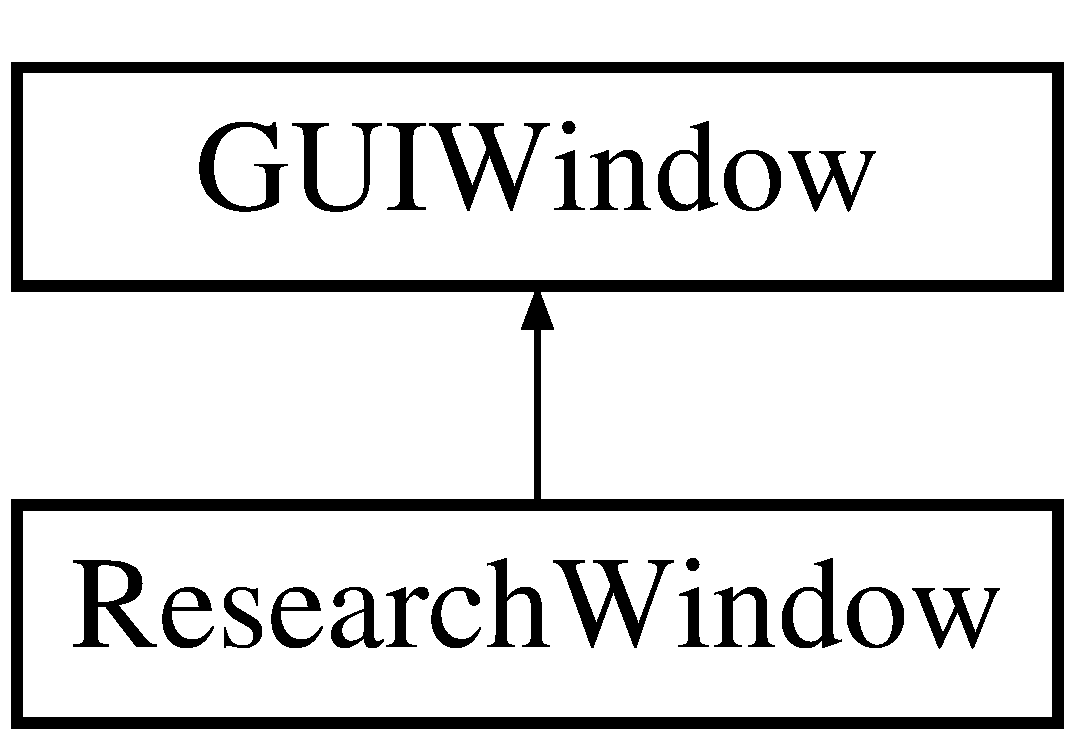
\includegraphics[height=2.000000cm]{class_research_window}
\end{center}
\end{figure}
\subsection*{Public Member Functions}
\begin{DoxyCompactItemize}
\item 
\hyperlink{class_research_window_a269831a5df51bf25aa58a808aa90d8dd}{Research\+Window} ()
\begin{DoxyCompactList}\small\item\em Constructor. \end{DoxyCompactList}\item 
\hyperlink{class_research_window_a6bab33e0158b5084b5dfd4829505bdae}{$\sim$\+Research\+Window} ()=default
\begin{DoxyCompactList}\small\item\em Destructor. \end{DoxyCompactList}\item 
void \hyperlink{class_research_window_a72fc4f35e0edcf7a806b8d756d6ef6fa}{unlock} (tdt\+::uint, tdt\+::uint)
\begin{DoxyCompactList}\small\item\em Unlocks a single research point at a given position in the research table. \end{DoxyCompactList}\item 
void \hyperlink{class_research_window_a6c77d878fea0275317a1d6fca0a43208}{dummy\+\_\+unlock} (tdt\+::uint, tdt\+::uint)
\begin{DoxyCompactList}\small\item\em Unlocks a single research point without activating it. \end{DoxyCompactList}\item 
const std\+::array$<$ bool, 42 $>$ \& \hyperlink{class_research_window_a6e75e6eba35907b8f5b08c8a8d1185fc}{get\+\_\+unlocked} () const 
\begin{DoxyCompactList}\small\item\em Returns a reference to the unlock table, used for serialization. \end{DoxyCompactList}\item 
void \hyperlink{class_research_window_a52c1497a959cadc2ea2ccc99e38149bd}{show} (tdt\+::uint, tdt\+::uint, bool=true)
\begin{DoxyCompactList}\small\item\em Shows a single research point at a given position in the research table. \end{DoxyCompactList}\item 
void \hyperlink{class_research_window_afaa2f334ffaaa466661132787b6cf73d}{free\+\_\+research} ()
\begin{DoxyCompactList}\small\item\em Cheat that changes the price of any research to 0. \end{DoxyCompactList}\item 
void \hyperlink{class_research_window_ad7550456fcac7b8eddadd9070161e755}{research\+\_\+all} ()
\begin{DoxyCompactList}\small\item\em Cheat that unlocks all research points. \end{DoxyCompactList}\item 
void \hyperlink{class_research_window_a47234d07778e8f3a29b0be59ce6c275f}{reset\+\_\+research} ()
\begin{DoxyCompactList}\small\item\em Resets the research state so that all items can be unlocked again. \end{DoxyCompactList}\end{DoxyCompactItemize}
\subsection*{Protected Member Functions}
\begin{DoxyCompactItemize}
\item 
void \hyperlink{class_research_window_ac47f66b9c25ddf9076c68196296120f9}{init\+\_\+} () override
\begin{DoxyCompactList}\small\item\em Initializes this window. \end{DoxyCompactList}\end{DoxyCompactItemize}
\subsection*{Private Member Functions}
\begin{DoxyCompactItemize}
\item 
tdt\+::uint \hyperlink{class_research_window_a938072590a252d02391883d7cdc9236b}{get\+\_\+price\+\_\+} (tdt\+::uint, tdt\+::uint)
\begin{DoxyCompactList}\small\item\em Returns the price in gold of a research point at the given position in the research table. \end{DoxyCompactList}\item 
bool \hyperlink{class_research_window_a016e751972256ac1832bed5c4cdabc75}{is\+\_\+unlocked\+\_\+} (tdt\+::uint, tdt\+::uint)
\begin{DoxyCompactList}\small\item\em Returns true if the research point at the given position is unlocked, false otherwise. \end{DoxyCompactList}\end{DoxyCompactItemize}
\subsection*{Private Attributes}
\begin{DoxyCompactItemize}
\item 
\hyperlink{classlpp_1_1_script}{lpp\+::\+Script} $\ast$ \hyperlink{class_research_window_af7f3013563f378a37e3b70c8fea0b555}{script\+\_\+}
\begin{DoxyCompactList}\small\item\em Pointer to the Lua Script used for easier access. \end{DoxyCompactList}\item 
const tdt\+::uint \hyperlink{class_research_window_aae4b998d4c40d8f05029968abb783c83}{rows\+\_\+} \{6\}
\begin{DoxyCompactList}\small\item\em Number of rows that the research table has. \end{DoxyCompactList}\item 
const tdt\+::uint \hyperlink{class_research_window_a52c91c5c4aded859123aa455b57820e1}{cols\+\_\+} \{7\}
\begin{DoxyCompactList}\small\item\em Number of columns that the research table has. \end{DoxyCompactList}\item 
std\+::array$<$ tdt\+::uint, 42 $>$ \hyperlink{class_research_window_afee1be8c37a9c599b2d56a12258f1a8f}{prices\+\_\+}
\begin{DoxyCompactList}\small\item\em Contains prices of the individual research points. \end{DoxyCompactList}\item 
std\+::array$<$ bool, 42 $>$ \hyperlink{class_research_window_a7e531797d054408609f43d633a43c07c}{unlocked\+\_\+}
\begin{DoxyCompactList}\small\item\em Contains information about the lock status of the individual research points. \end{DoxyCompactList}\end{DoxyCompactItemize}
\subsection*{Friends}
\begin{DoxyCompactItemize}
\item 
class {\bfseries Game\+Serializer}\hypertarget{class_research_window_a6f4a2258d01e962995f3a4743b711864}{}\label{class_research_window_a6f4a2258d01e962995f3a4743b711864}

\end{DoxyCompactItemize}
\subsection*{Additional Inherited Members}


\subsection{Detailed Description}
Class that represents the research window in the game, which allows the player to unlock new buildings and spells. 

\begin{DoxyNote}{Note}
Because this class is so tightly bound to Lua, the indices have to be adjusted when accessing the prices\+\_\+ and unlocked\+\_\+ arrays, since Lua uses indices starting at one when handling arrays. 
\end{DoxyNote}


Definition at line 18 of file Research\+Window.\+hpp.



\subsection{Constructor \& Destructor Documentation}
\index{Research\+Window@{Research\+Window}!Research\+Window@{Research\+Window}}
\index{Research\+Window@{Research\+Window}!Research\+Window@{Research\+Window}}
\subsubsection[{\texorpdfstring{Research\+Window()}{ResearchWindow()}}]{\setlength{\rightskip}{0pt plus 5cm}Research\+Window\+::\+Research\+Window (
\begin{DoxyParamCaption}
{}
\end{DoxyParamCaption}
)}\hypertarget{class_research_window_a269831a5df51bf25aa58a808aa90d8dd}{}\label{class_research_window_a269831a5df51bf25aa58a808aa90d8dd}


Constructor. 



Definition at line 6 of file Research\+Window.\+cpp.

\index{Research\+Window@{Research\+Window}!````~Research\+Window@{$\sim$\+Research\+Window}}
\index{````~Research\+Window@{$\sim$\+Research\+Window}!Research\+Window@{Research\+Window}}
\subsubsection[{\texorpdfstring{$\sim$\+Research\+Window()=default}{~ResearchWindow()=default}}]{\setlength{\rightskip}{0pt plus 5cm}Research\+Window\+::$\sim$\+Research\+Window (
\begin{DoxyParamCaption}
{}
\end{DoxyParamCaption}
)\hspace{0.3cm}{\ttfamily [default]}}\hypertarget{class_research_window_a6bab33e0158b5084b5dfd4829505bdae}{}\label{class_research_window_a6bab33e0158b5084b5dfd4829505bdae}


Destructor. 



\subsection{Member Function Documentation}
\index{Research\+Window@{Research\+Window}!dummy\+\_\+unlock@{dummy\+\_\+unlock}}
\index{dummy\+\_\+unlock@{dummy\+\_\+unlock}!Research\+Window@{Research\+Window}}
\subsubsection[{\texorpdfstring{dummy\+\_\+unlock(tdt\+::uint, tdt\+::uint)}{dummy_unlock(tdt::uint, tdt::uint)}}]{\setlength{\rightskip}{0pt plus 5cm}void Research\+Window\+::dummy\+\_\+unlock (
\begin{DoxyParamCaption}
\item[{tdt\+::uint}]{i, }
\item[{tdt\+::uint}]{j}
\end{DoxyParamCaption}
)}\hypertarget{class_research_window_a6c77d878fea0275317a1d6fca0a43208}{}\label{class_research_window_a6c77d878fea0275317a1d6fca0a43208}


Unlocks a single research point without activating it. 

Used for serialization. 
\begin{DoxyParams}{Parameters}
{\em Row} & number. \\
\hline
{\em Column} & number. \\
\hline
\end{DoxyParams}


Definition at line 28 of file Research\+Window.\+cpp.

\index{Research\+Window@{Research\+Window}!free\+\_\+research@{free\+\_\+research}}
\index{free\+\_\+research@{free\+\_\+research}!Research\+Window@{Research\+Window}}
\subsubsection[{\texorpdfstring{free\+\_\+research()}{free_research()}}]{\setlength{\rightskip}{0pt plus 5cm}void Research\+Window\+::free\+\_\+research (
\begin{DoxyParamCaption}
{}
\end{DoxyParamCaption}
)}\hypertarget{class_research_window_afaa2f334ffaaa466661132787b6cf73d}{}\label{class_research_window_afaa2f334ffaaa466661132787b6cf73d}


Cheat that changes the price of any research to 0. 



Definition at line 51 of file Research\+Window.\+cpp.

\index{Research\+Window@{Research\+Window}!get\+\_\+price\+\_\+@{get\+\_\+price\+\_\+}}
\index{get\+\_\+price\+\_\+@{get\+\_\+price\+\_\+}!Research\+Window@{Research\+Window}}
\subsubsection[{\texorpdfstring{get\+\_\+price\+\_\+(tdt\+::uint, tdt\+::uint)}{get_price_(tdt::uint, tdt::uint)}}]{\setlength{\rightskip}{0pt plus 5cm}tdt\+::uint Research\+Window\+::get\+\_\+price\+\_\+ (
\begin{DoxyParamCaption}
\item[{tdt\+::uint}]{i, }
\item[{tdt\+::uint}]{j}
\end{DoxyParamCaption}
)\hspace{0.3cm}{\ttfamily [private]}}\hypertarget{class_research_window_a938072590a252d02391883d7cdc9236b}{}\label{class_research_window_a938072590a252d02391883d7cdc9236b}


Returns the price in gold of a research point at the given position in the research table. 


\begin{DoxyParams}{Parameters}
{\em Row} & number. \\
\hline
{\em Column} & number. \\
\hline
\end{DoxyParams}


Definition at line 154 of file Research\+Window.\+cpp.

\index{Research\+Window@{Research\+Window}!get\+\_\+unlocked@{get\+\_\+unlocked}}
\index{get\+\_\+unlocked@{get\+\_\+unlocked}!Research\+Window@{Research\+Window}}
\subsubsection[{\texorpdfstring{get\+\_\+unlocked() const }{get_unlocked() const }}]{\setlength{\rightskip}{0pt plus 5cm}const std\+::array$<$ bool, 42 $>$ \& Research\+Window\+::get\+\_\+unlocked (
\begin{DoxyParamCaption}
{}
\end{DoxyParamCaption}
) const}\hypertarget{class_research_window_a6e75e6eba35907b8f5b08c8a8d1185fc}{}\label{class_research_window_a6e75e6eba35907b8f5b08c8a8d1185fc}


Returns a reference to the unlock table, used for serialization. 



Definition at line 41 of file Research\+Window.\+cpp.

\index{Research\+Window@{Research\+Window}!init\+\_\+@{init\+\_\+}}
\index{init\+\_\+@{init\+\_\+}!Research\+Window@{Research\+Window}}
\subsubsection[{\texorpdfstring{init\+\_\+() override}{init_() override}}]{\setlength{\rightskip}{0pt plus 5cm}void Research\+Window\+::init\+\_\+ (
\begin{DoxyParamCaption}
{}
\end{DoxyParamCaption}
)\hspace{0.3cm}{\ttfamily [override]}, {\ttfamily [protected]}, {\ttfamily [virtual]}}\hypertarget{class_research_window_ac47f66b9c25ddf9076c68196296120f9}{}\label{class_research_window_ac47f66b9c25ddf9076c68196296120f9}


Initializes this window. 

Makes sure all buttons can be used in the beggining.

Research button initialization.

\begin{DoxyNote}{Note}
Alfisko\+Skin does not have tooltip support, maybe create own skin? butt-\/$>$set\+Tooltip\+Text( script\+\_\+-\/$>$call$<$std\+::string, tdt\+::uint, tdt\+::uint$>$( \char`\"{}game.\+gui.\+research.\+get\+\_\+tooltip\char`\"{}, i, j ) ); 
\end{DoxyNote}


Implements \hyperlink{class_g_u_i_window_a2a7c011363f401a57a26cc7c7652bdfd}{G\+U\+I\+Window}.



Definition at line 95 of file Research\+Window.\+cpp.

\index{Research\+Window@{Research\+Window}!is\+\_\+unlocked\+\_\+@{is\+\_\+unlocked\+\_\+}}
\index{is\+\_\+unlocked\+\_\+@{is\+\_\+unlocked\+\_\+}!Research\+Window@{Research\+Window}}
\subsubsection[{\texorpdfstring{is\+\_\+unlocked\+\_\+(tdt\+::uint, tdt\+::uint)}{is_unlocked_(tdt::uint, tdt::uint)}}]{\setlength{\rightskip}{0pt plus 5cm}bool Research\+Window\+::is\+\_\+unlocked\+\_\+ (
\begin{DoxyParamCaption}
\item[{tdt\+::uint}]{i, }
\item[{tdt\+::uint}]{j}
\end{DoxyParamCaption}
)\hspace{0.3cm}{\ttfamily [private]}}\hypertarget{class_research_window_a016e751972256ac1832bed5c4cdabc75}{}\label{class_research_window_a016e751972256ac1832bed5c4cdabc75}


Returns true if the research point at the given position is unlocked, false otherwise. 


\begin{DoxyParams}{Parameters}
{\em Row} & number. \\
\hline
{\em Column} & number. \\
\hline
\end{DoxyParams}


Definition at line 163 of file Research\+Window.\+cpp.

\index{Research\+Window@{Research\+Window}!research\+\_\+all@{research\+\_\+all}}
\index{research\+\_\+all@{research\+\_\+all}!Research\+Window@{Research\+Window}}
\subsubsection[{\texorpdfstring{research\+\_\+all()}{research_all()}}]{\setlength{\rightskip}{0pt plus 5cm}void Research\+Window\+::research\+\_\+all (
\begin{DoxyParamCaption}
{}
\end{DoxyParamCaption}
)}\hypertarget{class_research_window_ad7550456fcac7b8eddadd9070161e755}{}\label{class_research_window_ad7550456fcac7b8eddadd9070161e755}


Cheat that unlocks all research points. 



Definition at line 57 of file Research\+Window.\+cpp.

\index{Research\+Window@{Research\+Window}!reset\+\_\+research@{reset\+\_\+research}}
\index{reset\+\_\+research@{reset\+\_\+research}!Research\+Window@{Research\+Window}}
\subsubsection[{\texorpdfstring{reset\+\_\+research()}{reset_research()}}]{\setlength{\rightskip}{0pt plus 5cm}void Research\+Window\+::reset\+\_\+research (
\begin{DoxyParamCaption}
{}
\end{DoxyParamCaption}
)}\hypertarget{class_research_window_a47234d07778e8f3a29b0be59ce6c275f}{}\label{class_research_window_a47234d07778e8f3a29b0be59ce6c275f}


Resets the research state so that all items can be unlocked again. 



Definition at line 68 of file Research\+Window.\+cpp.

\index{Research\+Window@{Research\+Window}!show@{show}}
\index{show@{show}!Research\+Window@{Research\+Window}}
\subsubsection[{\texorpdfstring{show(tdt\+::uint, tdt\+::uint, bool=true)}{show(tdt::uint, tdt::uint, bool=true)}}]{\setlength{\rightskip}{0pt plus 5cm}void Research\+Window\+::show (
\begin{DoxyParamCaption}
\item[{tdt\+::uint}]{i, }
\item[{tdt\+::uint}]{j, }
\item[{bool}]{val = {\ttfamily true}}
\end{DoxyParamCaption}
)}\hypertarget{class_research_window_a52c1497a959cadc2ea2ccc99e38149bd}{}\label{class_research_window_a52c1497a959cadc2ea2ccc99e38149bd}


Shows a single research point at a given position in the research table. 


\begin{DoxyParams}{Parameters}
{\em Row} & number. \\
\hline
{\em Column} & number. \\
\hline
{\em If} & true, shows the button, otherwise it hides it. \\
\hline
\end{DoxyParams}


Definition at line 46 of file Research\+Window.\+cpp.

\index{Research\+Window@{Research\+Window}!unlock@{unlock}}
\index{unlock@{unlock}!Research\+Window@{Research\+Window}}
\subsubsection[{\texorpdfstring{unlock(tdt\+::uint, tdt\+::uint)}{unlock(tdt::uint, tdt::uint)}}]{\setlength{\rightskip}{0pt plus 5cm}void Research\+Window\+::unlock (
\begin{DoxyParamCaption}
\item[{tdt\+::uint}]{i, }
\item[{tdt\+::uint}]{j}
\end{DoxyParamCaption}
)}\hypertarget{class_research_window_a72fc4f35e0edcf7a806b8d756d6ef6fa}{}\label{class_research_window_a72fc4f35e0edcf7a806b8d756d6ef6fa}


Unlocks a single research point at a given position in the research table. 


\begin{DoxyParams}{Parameters}
{\em Row} & number. \\
\hline
{\em Column} & number. \\
\hline
\end{DoxyParams}


Definition at line 10 of file Research\+Window.\+cpp.



\subsection{Member Data Documentation}
\index{Research\+Window@{Research\+Window}!cols\+\_\+@{cols\+\_\+}}
\index{cols\+\_\+@{cols\+\_\+}!Research\+Window@{Research\+Window}}
\subsubsection[{\texorpdfstring{cols\+\_\+}{cols_}}]{\setlength{\rightskip}{0pt plus 5cm}const tdt\+::uint Research\+Window\+::cols\+\_\+ \{7\}\hspace{0.3cm}{\ttfamily [private]}}\hypertarget{class_research_window_a52c91c5c4aded859123aa455b57820e1}{}\label{class_research_window_a52c91c5c4aded859123aa455b57820e1}


Number of columns that the research table has. 



Definition at line 115 of file Research\+Window.\+hpp.

\index{Research\+Window@{Research\+Window}!prices\+\_\+@{prices\+\_\+}}
\index{prices\+\_\+@{prices\+\_\+}!Research\+Window@{Research\+Window}}
\subsubsection[{\texorpdfstring{prices\+\_\+}{prices_}}]{\setlength{\rightskip}{0pt plus 5cm}std\+::array$<$tdt\+::uint, 42$>$ Research\+Window\+::prices\+\_\+\hspace{0.3cm}{\ttfamily [private]}}\hypertarget{class_research_window_afee1be8c37a9c599b2d56a12258f1a8f}{}\label{class_research_window_afee1be8c37a9c599b2d56a12258f1a8f}


Contains prices of the individual research points. 

Used to avoid unnecessary Lua lookups. 

Definition at line 121 of file Research\+Window.\+hpp.

\index{Research\+Window@{Research\+Window}!rows\+\_\+@{rows\+\_\+}}
\index{rows\+\_\+@{rows\+\_\+}!Research\+Window@{Research\+Window}}
\subsubsection[{\texorpdfstring{rows\+\_\+}{rows_}}]{\setlength{\rightskip}{0pt plus 5cm}const tdt\+::uint Research\+Window\+::rows\+\_\+ \{6\}\hspace{0.3cm}{\ttfamily [private]}}\hypertarget{class_research_window_aae4b998d4c40d8f05029968abb783c83}{}\label{class_research_window_aae4b998d4c40d8f05029968abb783c83}


Number of rows that the research table has. 



Definition at line 110 of file Research\+Window.\+hpp.

\index{Research\+Window@{Research\+Window}!script\+\_\+@{script\+\_\+}}
\index{script\+\_\+@{script\+\_\+}!Research\+Window@{Research\+Window}}
\subsubsection[{\texorpdfstring{script\+\_\+}{script_}}]{\setlength{\rightskip}{0pt plus 5cm}{\bf lpp\+::\+Script}$\ast$ Research\+Window\+::script\+\_\+\hspace{0.3cm}{\ttfamily [private]}}\hypertarget{class_research_window_af7f3013563f378a37e3b70c8fea0b555}{}\label{class_research_window_af7f3013563f378a37e3b70c8fea0b555}


Pointer to the Lua Script used for easier access. 



Definition at line 105 of file Research\+Window.\+hpp.

\index{Research\+Window@{Research\+Window}!unlocked\+\_\+@{unlocked\+\_\+}}
\index{unlocked\+\_\+@{unlocked\+\_\+}!Research\+Window@{Research\+Window}}
\subsubsection[{\texorpdfstring{unlocked\+\_\+}{unlocked_}}]{\setlength{\rightskip}{0pt plus 5cm}std\+::array$<$bool, 42$>$ Research\+Window\+::unlocked\+\_\+\hspace{0.3cm}{\ttfamily [private]}}\hypertarget{class_research_window_a7e531797d054408609f43d633a43c07c}{}\label{class_research_window_a7e531797d054408609f43d633a43c07c}


Contains information about the lock status of the individual research points. 

Used to avoid unnecessary Lua lookups. 

Definition at line 128 of file Research\+Window.\+hpp.



The documentation for this class was generated from the following files\+:\begin{DoxyCompactItemize}
\item 
gui/Research\+Window.\+hpp\item 
gui/Research\+Window.\+cpp\end{DoxyCompactItemize}

\hypertarget{structutil_1_1heuristic_1_1_r_u_n___a_w_a_y___h_e_u_r_i_s_t_i_c}{}\section{util\+:\+:heuristic\+:\+:R\+U\+N\+\_\+\+A\+W\+A\+Y\+\_\+\+H\+E\+U\+R\+I\+S\+T\+IC Struct Reference}
\label{structutil_1_1heuristic_1_1_r_u_n___a_w_a_y___h_e_u_r_i_s_t_i_c}\index{util\+::heuristic\+::\+R\+U\+N\+\_\+\+A\+W\+A\+Y\+\_\+\+H\+E\+U\+R\+I\+S\+T\+IC@{util\+::heuristic\+::\+R\+U\+N\+\_\+\+A\+W\+A\+Y\+\_\+\+H\+E\+U\+R\+I\+S\+T\+IC}}


Used by entities that want to run away from an enemy.  




{\ttfamily \#include $<$Pathfinding\+Algorithms.\+hpp$>$}

Inheritance diagram for util\+:\+:heuristic\+:\+:R\+U\+N\+\_\+\+A\+W\+A\+Y\+\_\+\+H\+E\+U\+R\+I\+S\+T\+IC\+:\begin{figure}[H]
\begin{center}
\leavevmode
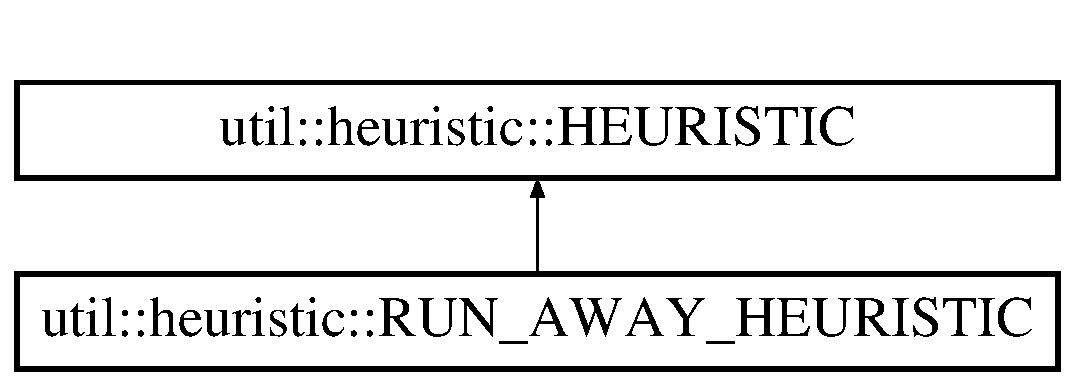
\includegraphics[height=2.000000cm]{structutil_1_1heuristic_1_1_r_u_n___a_w_a_y___h_e_u_r_i_s_t_i_c}
\end{center}
\end{figure}
\subsection*{Public Member Functions}
\begin{DoxyCompactItemize}
\item 
{\bfseries R\+U\+N\+\_\+\+A\+W\+A\+Y\+\_\+\+H\+E\+U\+R\+I\+S\+T\+IC} (\hyperlink{class_entity_system}{Entity\+System} \&ents, tdt\+::uint from)\hypertarget{structutil_1_1heuristic_1_1_r_u_n___a_w_a_y___h_e_u_r_i_s_t_i_c_a2b78448b2d225def225601ac2cbb8f8c}{}\label{structutil_1_1heuristic_1_1_r_u_n___a_w_a_y___h_e_u_r_i_s_t_i_c_a2b78448b2d225def225601ac2cbb8f8c}

\item 
tdt\+::real {\bfseries get\+\_\+cost} (tdt\+::uint id1, tdt\+::uint id2) override\hypertarget{structutil_1_1heuristic_1_1_r_u_n___a_w_a_y___h_e_u_r_i_s_t_i_c_a66af6c2d26e4f1a39a8104fe26e14ebd}{}\label{structutil_1_1heuristic_1_1_r_u_n___a_w_a_y___h_e_u_r_i_s_t_i_c_a66af6c2d26e4f1a39a8104fe26e14ebd}

\end{DoxyCompactItemize}
\subsection*{Private Attributes}
\begin{DoxyCompactItemize}
\item 
tdt\+::uint {\bfseries from\+\_\+}\hypertarget{structutil_1_1heuristic_1_1_r_u_n___a_w_a_y___h_e_u_r_i_s_t_i_c_a6db40574c55d644ee87513ddcbb0c69a}{}\label{structutil_1_1heuristic_1_1_r_u_n___a_w_a_y___h_e_u_r_i_s_t_i_c_a6db40574c55d644ee87513ddcbb0c69a}

\end{DoxyCompactItemize}
\subsection*{Additional Inherited Members}


\subsection{Detailed Description}
Used by entities that want to run away from an enemy. 

Definition at line 240 of file Pathfinding\+Algorithms.\+hpp.



The documentation for this struct was generated from the following file\+:\begin{DoxyCompactItemize}
\item 
tools/Pathfinding\+Algorithms.\+hpp\end{DoxyCompactItemize}

\hypertarget{classlpp_1_1_script}{}\section{lpp\+:\+:Script Class Reference}
\label{classlpp_1_1_script}\index{lpp\+::\+Script@{lpp\+::\+Script}}


Class representing a Lua script, allows to register C++ functions, load variables, call functions, execute strings containing Lua code and other functionalities.  




{\ttfamily \#include $<$Lpp\+Script.\+hpp$>$}

\subsection*{Public Types}
\begin{DoxyCompactItemize}
\item 
using {\bfseries state} = lua\+\_\+\+State $\ast$\hypertarget{classlpp_1_1_script_a13f260b1d630839b13881333bcd44188}{}\label{classlpp_1_1_script_a13f260b1d630839b13881333bcd44188}

\item 
using {\bfseries regs} = lua\+L\+\_\+\+Reg\hypertarget{classlpp_1_1_script_a090601b6d3da1285189245966234046c}{}\label{classlpp_1_1_script_a090601b6d3da1285189245966234046c}

\end{DoxyCompactItemize}
\subsection*{Public Member Functions}
\begin{DoxyCompactItemize}
\item 
\hyperlink{classlpp_1_1_script_a7f4bd859e2dd9925694e7b3bb004ce67}{Script} (const \hyperlink{classlpp_1_1_script}{Script} \&)=delete
\begin{DoxyCompactList}\small\item\em Copying this script might cause the Lua state get closed when one of the copies gets destroyed and would cause the game to be unable to use it\textquotesingle{}s scripting engine (and thus crashing probably). \end{DoxyCompactList}\item 
\hyperlink{classlpp_1_1_script_ad2e00e9ebbf4e78370bd21357ba01b36}{$\sim$\+Script} ()
\begin{DoxyCompactList}\small\item\em Destructor, closes the Lua virtual machine. \end{DoxyCompactList}\item 
state \hyperlink{classlpp_1_1_script_a2d4f9b1265f7866aa5991f69091b7265}{get\+\_\+state} ()
\begin{DoxyCompactList}\small\item\em Returns the lua state representing the Lua virtual machine. \end{DoxyCompactList}\item 
void \hyperlink{classlpp_1_1_script_a8e287a10f658161d9bf90ee3f39706b4}{execute} (const std\+::string \&)
\begin{DoxyCompactList}\small\item\em Executes a given string from within Lua. \end{DoxyCompactList}\item 
void \hyperlink{classlpp_1_1_script_a39d9522568a7187e65ebc20575ad6d4c}{register\+\_\+function} (const std\+::string \&, lua\+\_\+\+C\+Function)
\begin{DoxyCompactList}\small\item\em Registers a C++ function which can then be used from within Lua. \end{DoxyCompactList}\item 
void \hyperlink{classlpp_1_1_script_a14b6b2d01d21fe061cfcf5983cfd3e2f}{load} (const std\+::string \&)
\begin{DoxyCompactList}\small\item\em Loads, compiles and executes a Lua script. \end{DoxyCompactList}\item 
bool \hyperlink{classlpp_1_1_script_ae03581ef0b1ce4c639f2f592e332d3bd}{is\+\_\+nil} (const std\+::string \&)
\begin{DoxyCompactList}\small\item\em Returns true if a given value is nil, false otherwise. \end{DoxyCompactList}\item 
{\footnotesize template$<$typename T $>$ }\\T \hyperlink{classlpp_1_1_script_a183b83008d4b2647b0b45b4bf94f25bd}{get} (const std\+::string \&name)
\begin{DoxyCompactList}\small\item\em Retrieves and returns a value from Lua. \end{DoxyCompactList}\item 
{\footnotesize template$<$typename Result , typename... Args$>$ }\\Result \hyperlink{classlpp_1_1_script_a58c51f17a5ed784dca84a156da7d98ec}{call} (const std\+::string \&fname, Args...\+as)
\begin{DoxyCompactList}\small\item\em Calls a given Lua function. \end{DoxyCompactList}\item 
{\footnotesize template$<$typename Result $>$ }\\Result \hyperlink{classlpp_1_1_script_a2f11bea50dfdb331923f552ca42a4aec}{call} (const std\+::string \&fname)
\begin{DoxyCompactList}\small\item\em Calls a given Lua function. \end{DoxyCompactList}\item 
{\footnotesize template$<$typename T $>$ }\\void \hyperlink{classlpp_1_1_script_ad92d15b3c9342b9c455de30a3cf321df}{set} (const std\+::string \&name, T val)
\begin{DoxyCompactList}\small\item\em Sets a given variable to a given value. \end{DoxyCompactList}\item 
{\footnotesize template$<$typename T $>$ }\\std\+::vector$<$ T $>$ \hyperlink{classlpp_1_1_script_a8ca0dab497f114069dd28a14eab957aa}{get\+\_\+vector} (const std\+::string \&name)
\begin{DoxyCompactList}\small\item\em Retrieves a Lua array table (integer indexing) in the form of a C++ vector. \end{DoxyCompactList}\item 
std\+::string \hyperlink{classlpp_1_1_script_a232aa76e2307bf1fbd0e3e890edd3874}{get\+\_\+stack\+\_\+contents} ()
\begin{DoxyCompactList}\small\item\em Returns string representation of the Lua stack. \end{DoxyCompactList}\item 
void \hyperlink{classlpp_1_1_script_a2a97d7191cff462376326efb9e3ad841}{reload\+\_\+all\+\_\+scripts} ()
\begin{DoxyCompactList}\small\item\em Reloads all script files that have been previously loaded. \end{DoxyCompactList}\item 
{\footnotesize template$<$$>$ }\\void {\bfseries set} (const std\+::string \&name, bool val)\hypertarget{classlpp_1_1_script_a07d0738e7298bc93b98fcae4241fca85}{}\label{classlpp_1_1_script_a07d0738e7298bc93b98fcae4241fca85}

\end{DoxyCompactItemize}
\subsection*{Static Public Member Functions}
\begin{DoxyCompactItemize}
\item 
static \hyperlink{classlpp_1_1_script}{Script} \& \hyperlink{classlpp_1_1_script_a9ca5b255301a8e9a1aedc15e62fe677c}{instance} ()
\begin{DoxyCompactList}\small\item\em Returns a reference to the \hyperlink{classlpp_1_1_script}{lpp\+::\+Script} singleton. \end{DoxyCompactList}\end{DoxyCompactItemize}
\subsection*{Private Member Functions}
\begin{DoxyCompactItemize}
\item 
\hyperlink{classlpp_1_1_script_a5c7d3ac74a426de91e77b1f3791fda1e}{Script} ()
\begin{DoxyCompactList}\small\item\em Constructor, kept private because of the use of the singleton pattern. \end{DoxyCompactList}\item 
std\+::string \hyperlink{classlpp_1_1_script_af6fcf9309891444f435df96667c51a95}{get\+\_\+field\+\_\+to\+\_\+stack} (const std\+::string \&)
\begin{DoxyCompactList}\small\item\em Gets a nested value (inside a table hierarchy) on top of the stack and returns the name of the final variable (without table prefixes). \end{DoxyCompactList}\item 
void \hyperlink{classlpp_1_1_script_a96d4cb098566a4390d764cee2d7d0b70}{clear\+\_\+stack} ()
\begin{DoxyCompactList}\small\item\em Pops everything off the stack. \end{DoxyCompactList}\item 
{\footnotesize template$<$typename T $>$ }\\T \hyperlink{classlpp_1_1_script_a90226739c06be4b6665bc529a08636fa}{get\+\_\+} (const std\+::string \&name=\char`\"{}unknown\char`\"{})
\begin{DoxyCompactList}\small\item\em Returns the value stored on top of the stack. \end{DoxyCompactList}\item 
{\footnotesize template$<$typename Arg , typename... Args$>$ }\\int \hyperlink{classlpp_1_1_script_ae9a31ab88caf85834a400cd080bc55ec}{push\+\_\+args} (Arg a, Args...\+as)
\begin{DoxyCompactList}\small\item\em Pushed a variadic list of arguments onto the stack to be passed as arguments to a Lua function call, returns the amount of arguments pushed onto the stack. \end{DoxyCompactList}\item 
{\footnotesize template$<$typename Arg $>$ }\\int \hyperlink{classlpp_1_1_script_a9c83737f00a0613efa0276bc94ea47dd}{push\+\_\+args} (Arg a)
\begin{DoxyCompactList}\small\item\em Bottom case of the push\+\_\+args recursive call. \end{DoxyCompactList}\item 
{\footnotesize template$<$typename Arg $>$ }\\void \hyperlink{classlpp_1_1_script_a9ecaddf33b0978b245ebf787a22ea173}{push\+\_\+arg} (Arg a)
\begin{DoxyCompactList}\small\item\em Pushes a single value onto the Lua stack. \end{DoxyCompactList}\item 
{\footnotesize template$<$$>$ }\\int {\bfseries get\+\_\+} (const std\+::string \&name)\hypertarget{classlpp_1_1_script_a14decfe611481d7bbcedad5da49081ba}{}\label{classlpp_1_1_script_a14decfe611481d7bbcedad5da49081ba}

\item 
{\footnotesize template$<$$>$ }\\bool {\bfseries get\+\_\+} (const std\+::string \&name)\hypertarget{classlpp_1_1_script_a085e23878a5e24c08ea1764750f1267a}{}\label{classlpp_1_1_script_a085e23878a5e24c08ea1764750f1267a}

\item 
{\footnotesize template$<$$>$ }\\void {\bfseries get\+\_\+} (const std\+::string \&name)\hypertarget{classlpp_1_1_script_a7fbc6d125505b00eff3217f948de50d7}{}\label{classlpp_1_1_script_a7fbc6d125505b00eff3217f948de50d7}

\item 
{\footnotesize template$<$$>$ }\\void \hyperlink{classlpp_1_1_script_a9eb70929df748e82de5b01884fab47af}{push\+\_\+arg} (int arg)
\begin{DoxyCompactList}\small\item\em Specializations of the method \hyperlink{classlpp_1_1_script_a9ecaddf33b0978b245ebf787a22ea173}{lpp\+::\+Script\+::push\+\_\+arg}, which pushes a single function argument onto the Lua stack. \end{DoxyCompactList}\item 
{\footnotesize template$<$$>$ }\\void {\bfseries push\+\_\+arg} (float arg)\hypertarget{classlpp_1_1_script_a7bbb0cfd6cd1c3d6192f72d7c8fd3c55}{}\label{classlpp_1_1_script_a7bbb0cfd6cd1c3d6192f72d7c8fd3c55}

\item 
{\footnotesize template$<$$>$ }\\void {\bfseries push\+\_\+arg} (bool arg)\hypertarget{classlpp_1_1_script_a7338f6a1d447a3da273085c566f30645}{}\label{classlpp_1_1_script_a7338f6a1d447a3da273085c566f30645}

\end{DoxyCompactItemize}
\subsection*{Private Attributes}
\begin{DoxyCompactItemize}
\item 
state \hyperlink{classlpp_1_1_script_a1bf67bd893423cb0e6cc4121957ff33d}{L}
\begin{DoxyCompactList}\small\item\em Lua state representing the Lua virtual machine. \end{DoxyCompactList}\item 
std\+::set$<$ std\+::string $>$ \hyperlink{classlpp_1_1_script_abf7d2cb96488dea057fd2d9d3fedb144}{loaded\+\_\+scripts\+\_\+}
\begin{DoxyCompactList}\small\item\em Containes the names of all scripts loaded during the current runtime. \end{DoxyCompactList}\end{DoxyCompactItemize}


\subsection{Detailed Description}
Class representing a Lua script, allows to register C++ functions, load variables, call functions, execute strings containing Lua code and other functionalities. 

Definition at line 18 of file Lpp\+Script.\+hpp.



\subsection{Constructor \& Destructor Documentation}
\index{lpp\+::\+Script@{lpp\+::\+Script}!Script@{Script}}
\index{Script@{Script}!lpp\+::\+Script@{lpp\+::\+Script}}
\subsubsection[{\texorpdfstring{Script(const Script \&)=delete}{Script(const Script &)=delete}}]{\setlength{\rightskip}{0pt plus 5cm}lpp\+::\+Script\+::\+Script (
\begin{DoxyParamCaption}
\item[{const {\bf Script} \&}]{}
\end{DoxyParamCaption}
)\hspace{0.3cm}{\ttfamily [delete]}}\hypertarget{classlpp_1_1_script_a7f4bd859e2dd9925694e7b3bb004ce67}{}\label{classlpp_1_1_script_a7f4bd859e2dd9925694e7b3bb004ce67}


Copying this script might cause the Lua state get closed when one of the copies gets destroyed and would cause the game to be unable to use it\textquotesingle{}s scripting engine (and thus crashing probably). 

\index{lpp\+::\+Script@{lpp\+::\+Script}!````~Script@{$\sim$\+Script}}
\index{````~Script@{$\sim$\+Script}!lpp\+::\+Script@{lpp\+::\+Script}}
\subsubsection[{\texorpdfstring{$\sim$\+Script()}{~Script()}}]{\setlength{\rightskip}{0pt plus 5cm}lpp\+::\+Script\+::$\sim$\+Script (
\begin{DoxyParamCaption}
{}
\end{DoxyParamCaption}
)\hspace{0.3cm}{\ttfamily [inline]}}\hypertarget{classlpp_1_1_script_ad2e00e9ebbf4e78370bd21357ba01b36}{}\label{classlpp_1_1_script_ad2e00e9ebbf4e78370bd21357ba01b36}


Destructor, closes the Lua virtual machine. 



Definition at line 34 of file Lpp\+Script.\+hpp.

\index{lpp\+::\+Script@{lpp\+::\+Script}!Script@{Script}}
\index{Script@{Script}!lpp\+::\+Script@{lpp\+::\+Script}}
\subsubsection[{\texorpdfstring{Script()}{Script()}}]{\setlength{\rightskip}{0pt plus 5cm}lpp\+::\+Script\+::\+Script (
\begin{DoxyParamCaption}
{}
\end{DoxyParamCaption}
)\hspace{0.3cm}{\ttfamily [private]}}\hypertarget{classlpp_1_1_script_a5c7d3ac74a426de91e77b1f3791fda1e}{}\label{classlpp_1_1_script_a5c7d3ac74a426de91e77b1f3791fda1e}


Constructor, kept private because of the use of the singleton pattern. 

\hyperlink{classlpp_1_1_script}{lpp\+::\+Script} definitions\+: 

Definition at line 7 of file Lpp\+Script.\+cpp.



\subsection{Member Function Documentation}
\index{lpp\+::\+Script@{lpp\+::\+Script}!call@{call}}
\index{call@{call}!lpp\+::\+Script@{lpp\+::\+Script}}
\subsubsection[{\texorpdfstring{call(const std\+::string \&fname, Args...\+as)}{call(const std::string &fname, Args...as)}}]{\setlength{\rightskip}{0pt plus 5cm}template$<$typename Result , typename... Args$>$ Result lpp\+::\+Script\+::call (
\begin{DoxyParamCaption}
\item[{const std\+::string \&}]{fname, }
\item[{Args...}]{as}
\end{DoxyParamCaption}
)\hspace{0.3cm}{\ttfamily [inline]}}\hypertarget{classlpp_1_1_script_a58c51f17a5ed784dca84a156da7d98ec}{}\label{classlpp_1_1_script_a58c51f17a5ed784dca84a156da7d98ec}


Calls a given Lua function. 


\begin{DoxyParams}{Parameters}
{\em Name} & of the function. \\
\hline
{\em Variadic} & list of arguments that are passed to the function. \\
\hline
\end{DoxyParams}


Definition at line 99 of file Lpp\+Script.\+hpp.

\index{lpp\+::\+Script@{lpp\+::\+Script}!call@{call}}
\index{call@{call}!lpp\+::\+Script@{lpp\+::\+Script}}
\subsubsection[{\texorpdfstring{call(const std\+::string \&fname)}{call(const std::string &fname)}}]{\setlength{\rightskip}{0pt plus 5cm}template$<$typename Result $>$ Result lpp\+::\+Script\+::call (
\begin{DoxyParamCaption}
\item[{const std\+::string \&}]{fname}
\end{DoxyParamCaption}
)\hspace{0.3cm}{\ttfamily [inline]}}\hypertarget{classlpp_1_1_script_a2f11bea50dfdb331923f552ca42a4aec}{}\label{classlpp_1_1_script_a2f11bea50dfdb331923f552ca42a4aec}


Calls a given Lua function. 


\begin{DoxyParams}{Parameters}
{\em Name} & of the function. \\
\hline
\end{DoxyParams}


Definition at line 121 of file Lpp\+Script.\+hpp.

\index{lpp\+::\+Script@{lpp\+::\+Script}!clear\+\_\+stack@{clear\+\_\+stack}}
\index{clear\+\_\+stack@{clear\+\_\+stack}!lpp\+::\+Script@{lpp\+::\+Script}}
\subsubsection[{\texorpdfstring{clear\+\_\+stack()}{clear_stack()}}]{\setlength{\rightskip}{0pt plus 5cm}void lpp\+::\+Script\+::clear\+\_\+stack (
\begin{DoxyParamCaption}
{}
\end{DoxyParamCaption}
)\hspace{0.3cm}{\ttfamily [private]}}\hypertarget{classlpp_1_1_script_a96d4cb098566a4390d764cee2d7d0b70}{}\label{classlpp_1_1_script_a96d4cb098566a4390d764cee2d7d0b70}


Pops everything off the stack. 



Definition at line 66 of file Lpp\+Script.\+cpp.

\index{lpp\+::\+Script@{lpp\+::\+Script}!execute@{execute}}
\index{execute@{execute}!lpp\+::\+Script@{lpp\+::\+Script}}
\subsubsection[{\texorpdfstring{execute(const std\+::string \&)}{execute(const std::string &)}}]{\setlength{\rightskip}{0pt plus 5cm}void lpp\+::\+Script\+::execute (
\begin{DoxyParamCaption}
\item[{const std\+::string \&}]{command}
\end{DoxyParamCaption}
)}\hypertarget{classlpp_1_1_script_a8e287a10f658161d9bf90ee3f39706b4}{}\label{classlpp_1_1_script_a8e287a10f658161d9bf90ee3f39706b4}


Executes a given string from within Lua. 


\begin{DoxyParams}{Parameters}
{\em String} & containing commands to be executed. \\
\hline
\end{DoxyParams}


Definition at line 14 of file Lpp\+Script.\+cpp.

\index{lpp\+::\+Script@{lpp\+::\+Script}!get@{get}}
\index{get@{get}!lpp\+::\+Script@{lpp\+::\+Script}}
\subsubsection[{\texorpdfstring{get(const std\+::string \&name)}{get(const std::string &name)}}]{\setlength{\rightskip}{0pt plus 5cm}template$<$typename T $>$ T lpp\+::\+Script\+::get (
\begin{DoxyParamCaption}
\item[{const std\+::string \&}]{name}
\end{DoxyParamCaption}
)\hspace{0.3cm}{\ttfamily [inline]}}\hypertarget{classlpp_1_1_script_a183b83008d4b2647b0b45b4bf94f25bd}{}\label{classlpp_1_1_script_a183b83008d4b2647b0b45b4bf94f25bd}


Retrieves and returns a value from Lua. 


\begin{DoxyParams}{Parameters}
{\em Name} & of the variable containing the desired value. \\
\hline
\end{DoxyParams}


Definition at line 74 of file Lpp\+Script.\+hpp.

\index{lpp\+::\+Script@{lpp\+::\+Script}!get\+\_\+@{get\+\_\+}}
\index{get\+\_\+@{get\+\_\+}!lpp\+::\+Script@{lpp\+::\+Script}}
\subsubsection[{\texorpdfstring{get\+\_\+(const std\+::string \&name=""unknown"")}{get_(const std::string &name="unknown")}}]{\setlength{\rightskip}{0pt plus 5cm}template$<$typename T $>$ T lpp\+::\+Script\+::get\+\_\+ (
\begin{DoxyParamCaption}
\item[{const std\+::string \&}]{name = {\ttfamily \char`\"{}unknown\char`\"{}}}
\end{DoxyParamCaption}
)\hspace{0.3cm}{\ttfamily [private]}}\hypertarget{classlpp_1_1_script_a90226739c06be4b6665bc529a08636fa}{}\label{classlpp_1_1_script_a90226739c06be4b6665bc529a08636fa}


Returns the value stored on top of the stack. 

\index{lpp\+::\+Script@{lpp\+::\+Script}!get\+\_\+field\+\_\+to\+\_\+stack@{get\+\_\+field\+\_\+to\+\_\+stack}}
\index{get\+\_\+field\+\_\+to\+\_\+stack@{get\+\_\+field\+\_\+to\+\_\+stack}!lpp\+::\+Script@{lpp\+::\+Script}}
\subsubsection[{\texorpdfstring{get\+\_\+field\+\_\+to\+\_\+stack(const std\+::string \&)}{get_field_to_stack(const std::string &)}}]{\setlength{\rightskip}{0pt plus 5cm}std\+::string lpp\+::\+Script\+::get\+\_\+field\+\_\+to\+\_\+stack (
\begin{DoxyParamCaption}
\item[{const std\+::string \&}]{name}
\end{DoxyParamCaption}
)\hspace{0.3cm}{\ttfamily [private]}}\hypertarget{classlpp_1_1_script_af6fcf9309891444f435df96667c51a95}{}\label{classlpp_1_1_script_af6fcf9309891444f435df96667c51a95}


Gets a nested value (inside a table hierarchy) on top of the stack and returns the name of the final variable (without table prefixes). 


\begin{DoxyParams}{Parameters}
{\em Full} & name of the variable. \\
\hline
\end{DoxyParams}


Definition at line 47 of file Lpp\+Script.\+cpp.

\index{lpp\+::\+Script@{lpp\+::\+Script}!get\+\_\+stack\+\_\+contents@{get\+\_\+stack\+\_\+contents}}
\index{get\+\_\+stack\+\_\+contents@{get\+\_\+stack\+\_\+contents}!lpp\+::\+Script@{lpp\+::\+Script}}
\subsubsection[{\texorpdfstring{get\+\_\+stack\+\_\+contents()}{get_stack_contents()}}]{\setlength{\rightskip}{0pt plus 5cm}std\+::string lpp\+::\+Script\+::get\+\_\+stack\+\_\+contents (
\begin{DoxyParamCaption}
{}
\end{DoxyParamCaption}
)}\hypertarget{classlpp_1_1_script_a232aa76e2307bf1fbd0e3e890edd3874}{}\label{classlpp_1_1_script_a232aa76e2307bf1fbd0e3e890edd3874}


Returns string representation of the Lua stack. 



Definition at line 72 of file Lpp\+Script.\+cpp.

\index{lpp\+::\+Script@{lpp\+::\+Script}!get\+\_\+state@{get\+\_\+state}}
\index{get\+\_\+state@{get\+\_\+state}!lpp\+::\+Script@{lpp\+::\+Script}}
\subsubsection[{\texorpdfstring{get\+\_\+state()}{get_state()}}]{\setlength{\rightskip}{0pt plus 5cm}state lpp\+::\+Script\+::get\+\_\+state (
\begin{DoxyParamCaption}
{}
\end{DoxyParamCaption}
)\hspace{0.3cm}{\ttfamily [inline]}}\hypertarget{classlpp_1_1_script_a2d4f9b1265f7866aa5991f69091b7265}{}\label{classlpp_1_1_script_a2d4f9b1265f7866aa5991f69091b7265}


Returns the lua state representing the Lua virtual machine. 



Definition at line 39 of file Lpp\+Script.\+hpp.

\index{lpp\+::\+Script@{lpp\+::\+Script}!get\+\_\+vector@{get\+\_\+vector}}
\index{get\+\_\+vector@{get\+\_\+vector}!lpp\+::\+Script@{lpp\+::\+Script}}
\subsubsection[{\texorpdfstring{get\+\_\+vector(const std\+::string \&name)}{get_vector(const std::string &name)}}]{\setlength{\rightskip}{0pt plus 5cm}template$<$typename T $>$ std\+::vector$<$T$>$ lpp\+::\+Script\+::get\+\_\+vector (
\begin{DoxyParamCaption}
\item[{const std\+::string \&}]{name}
\end{DoxyParamCaption}
)\hspace{0.3cm}{\ttfamily [inline]}}\hypertarget{classlpp_1_1_script_a8ca0dab497f114069dd28a14eab957aa}{}\label{classlpp_1_1_script_a8ca0dab497f114069dd28a14eab957aa}


Retrieves a Lua array table (integer indexing) in the form of a C++ vector. 


\begin{DoxyParams}{Parameters}
{\em Name} & of the array. \\
\hline
\end{DoxyParams}


Definition at line 153 of file Lpp\+Script.\+hpp.

\index{lpp\+::\+Script@{lpp\+::\+Script}!instance@{instance}}
\index{instance@{instance}!lpp\+::\+Script@{lpp\+::\+Script}}
\subsubsection[{\texorpdfstring{instance()}{instance()}}]{\setlength{\rightskip}{0pt plus 5cm}{\bf lpp\+::\+Script} \& lpp\+::\+Script\+::instance (
\begin{DoxyParamCaption}
{}
\end{DoxyParamCaption}
)\hspace{0.3cm}{\ttfamily [static]}}\hypertarget{classlpp_1_1_script_a9ca5b255301a8e9a1aedc15e62fe677c}{}\label{classlpp_1_1_script_a9ca5b255301a8e9a1aedc15e62fe677c}


Returns a reference to the \hyperlink{classlpp_1_1_script}{lpp\+::\+Script} singleton. 



Definition at line 105 of file Lpp\+Script.\+cpp.

\index{lpp\+::\+Script@{lpp\+::\+Script}!is\+\_\+nil@{is\+\_\+nil}}
\index{is\+\_\+nil@{is\+\_\+nil}!lpp\+::\+Script@{lpp\+::\+Script}}
\subsubsection[{\texorpdfstring{is\+\_\+nil(const std\+::string \&)}{is_nil(const std::string &)}}]{\setlength{\rightskip}{0pt plus 5cm}bool lpp\+::\+Script\+::is\+\_\+nil (
\begin{DoxyParamCaption}
\item[{const std\+::string \&}]{name}
\end{DoxyParamCaption}
)}\hypertarget{classlpp_1_1_script_ae03581ef0b1ce4c639f2f592e332d3bd}{}\label{classlpp_1_1_script_ae03581ef0b1ce4c639f2f592e332d3bd}


Returns true if a given value is nil, false otherwise. 


\begin{DoxyParams}{Parameters}
{\em Name} & of the variable containing the desired value. \\
\hline
\end{DoxyParams}


Definition at line 34 of file Lpp\+Script.\+cpp.

\index{lpp\+::\+Script@{lpp\+::\+Script}!load@{load}}
\index{load@{load}!lpp\+::\+Script@{lpp\+::\+Script}}
\subsubsection[{\texorpdfstring{load(const std\+::string \&)}{load(const std::string &)}}]{\setlength{\rightskip}{0pt plus 5cm}void lpp\+::\+Script\+::load (
\begin{DoxyParamCaption}
\item[{const std\+::string \&}]{fname}
\end{DoxyParamCaption}
)}\hypertarget{classlpp_1_1_script_a14b6b2d01d21fe061cfcf5983cfd3e2f}{}\label{classlpp_1_1_script_a14b6b2d01d21fe061cfcf5983cfd3e2f}


Loads, compiles and executes a Lua script. 


\begin{DoxyParams}{Parameters}
{\em Name} & of the script file. \\
\hline
\end{DoxyParams}


Definition at line 25 of file Lpp\+Script.\+cpp.

\index{lpp\+::\+Script@{lpp\+::\+Script}!push\+\_\+arg@{push\+\_\+arg}}
\index{push\+\_\+arg@{push\+\_\+arg}!lpp\+::\+Script@{lpp\+::\+Script}}
\subsubsection[{\texorpdfstring{push\+\_\+arg(\+Arg a)}{push_arg(Arg a)}}]{\setlength{\rightskip}{0pt plus 5cm}template$<$typename Arg $>$ void lpp\+::\+Script\+::push\+\_\+arg (
\begin{DoxyParamCaption}
\item[{Arg}]{a}
\end{DoxyParamCaption}
)\hspace{0.3cm}{\ttfamily [inline]}, {\ttfamily [private]}}\hypertarget{classlpp_1_1_script_a9ecaddf33b0978b245ebf787a22ea173}{}\label{classlpp_1_1_script_a9ecaddf33b0978b245ebf787a22ea173}


Pushes a single value onto the Lua stack. 


\begin{DoxyParams}{Parameters}
{\em Value} & to be pushed. \\
\hline
\end{DoxyParams}
\begin{DoxyNote}{Note}
By default does nothing, only specialised versions push anything. 
\end{DoxyNote}


Definition at line 250 of file Lpp\+Script.\+hpp.

\index{lpp\+::\+Script@{lpp\+::\+Script}!push\+\_\+arg@{push\+\_\+arg}}
\index{push\+\_\+arg@{push\+\_\+arg}!lpp\+::\+Script@{lpp\+::\+Script}}
\subsubsection[{\texorpdfstring{push\+\_\+arg(int arg)}{push_arg(int arg)}}]{\setlength{\rightskip}{0pt plus 5cm}template$<$$>$ void lpp\+::\+Script\+::push\+\_\+arg (
\begin{DoxyParamCaption}
\item[{int}]{arg}
\end{DoxyParamCaption}
)\hspace{0.3cm}{\ttfamily [inline]}, {\ttfamily [private]}}\hypertarget{classlpp_1_1_script_a9eb70929df748e82de5b01884fab47af}{}\label{classlpp_1_1_script_a9eb70929df748e82de5b01884fab47af}


Specializations of the method \hyperlink{classlpp_1_1_script_a9ecaddf33b0978b245ebf787a22ea173}{lpp\+::\+Script\+::push\+\_\+arg}, which pushes a single function argument onto the Lua stack. 



Definition at line 370 of file Lpp\+Script.\+hpp.

\index{lpp\+::\+Script@{lpp\+::\+Script}!push\+\_\+args@{push\+\_\+args}}
\index{push\+\_\+args@{push\+\_\+args}!lpp\+::\+Script@{lpp\+::\+Script}}
\subsubsection[{\texorpdfstring{push\+\_\+args(\+Arg a, Args...\+as)}{push_args(Arg a, Args...as)}}]{\setlength{\rightskip}{0pt plus 5cm}template$<$typename Arg , typename... Args$>$ int lpp\+::\+Script\+::push\+\_\+args (
\begin{DoxyParamCaption}
\item[{Arg}]{a, }
\item[{Args...}]{as}
\end{DoxyParamCaption}
)\hspace{0.3cm}{\ttfamily [inline]}, {\ttfamily [private]}}\hypertarget{classlpp_1_1_script_ae9a31ab88caf85834a400cd080bc55ec}{}\label{classlpp_1_1_script_ae9a31ab88caf85834a400cd080bc55ec}


Pushed a variadic list of arguments onto the stack to be passed as arguments to a Lua function call, returns the amount of arguments pushed onto the stack. 


\begin{DoxyParams}{Parameters}
{\em First} & argument in the list. \\
\hline
{\em Tail} & argument list used in recursive call. \\
\hline
\end{DoxyParams}


Definition at line 226 of file Lpp\+Script.\+hpp.

\index{lpp\+::\+Script@{lpp\+::\+Script}!push\+\_\+args@{push\+\_\+args}}
\index{push\+\_\+args@{push\+\_\+args}!lpp\+::\+Script@{lpp\+::\+Script}}
\subsubsection[{\texorpdfstring{push\+\_\+args(\+Arg a)}{push_args(Arg a)}}]{\setlength{\rightskip}{0pt plus 5cm}template$<$typename Arg $>$ int lpp\+::\+Script\+::push\+\_\+args (
\begin{DoxyParamCaption}
\item[{Arg}]{a}
\end{DoxyParamCaption}
)\hspace{0.3cm}{\ttfamily [inline]}, {\ttfamily [private]}}\hypertarget{classlpp_1_1_script_a9c83737f00a0613efa0276bc94ea47dd}{}\label{classlpp_1_1_script_a9c83737f00a0613efa0276bc94ea47dd}


Bottom case of the push\+\_\+args recursive call. 


\begin{DoxyParams}{Parameters}
{\em Argument} & to be pushed onto the stack. \\
\hline
\end{DoxyParams}


Definition at line 237 of file Lpp\+Script.\+hpp.

\index{lpp\+::\+Script@{lpp\+::\+Script}!register\+\_\+function@{register\+\_\+function}}
\index{register\+\_\+function@{register\+\_\+function}!lpp\+::\+Script@{lpp\+::\+Script}}
\subsubsection[{\texorpdfstring{register\+\_\+function(const std\+::string \&, lua\+\_\+\+C\+Function)}{register_function(const std::string &, lua_CFunction)}}]{\setlength{\rightskip}{0pt plus 5cm}void lpp\+::\+Script\+::register\+\_\+function (
\begin{DoxyParamCaption}
\item[{const std\+::string \&}]{name, }
\item[{lua\+\_\+\+C\+Function}]{fn}
\end{DoxyParamCaption}
)}\hypertarget{classlpp_1_1_script_a39d9522568a7187e65ebc20575ad6d4c}{}\label{classlpp_1_1_script_a39d9522568a7187e65ebc20575ad6d4c}


Registers a C++ function which can then be used from within Lua. 


\begin{DoxyParams}{Parameters}
{\em Name} & of the function. \\
\hline
{\em Function} & to be registered, it has to have the signature int fname(lua\+\_\+\+State$\ast$) and return the number of results pushed onto the stack, arguments are on the stack. \\
\hline
\end{DoxyParams}


Definition at line 20 of file Lpp\+Script.\+cpp.

\index{lpp\+::\+Script@{lpp\+::\+Script}!reload\+\_\+all\+\_\+scripts@{reload\+\_\+all\+\_\+scripts}}
\index{reload\+\_\+all\+\_\+scripts@{reload\+\_\+all\+\_\+scripts}!lpp\+::\+Script@{lpp\+::\+Script}}
\subsubsection[{\texorpdfstring{reload\+\_\+all\+\_\+scripts()}{reload_all_scripts()}}]{\setlength{\rightskip}{0pt plus 5cm}void lpp\+::\+Script\+::reload\+\_\+all\+\_\+scripts (
\begin{DoxyParamCaption}
{}
\end{DoxyParamCaption}
)}\hypertarget{classlpp_1_1_script_a2a97d7191cff462376326efb9e3ad841}{}\label{classlpp_1_1_script_a2a97d7191cff462376326efb9e3ad841}


Reloads all script files that have been previously loaded. 



Definition at line 99 of file Lpp\+Script.\+cpp.

\index{lpp\+::\+Script@{lpp\+::\+Script}!set@{set}}
\index{set@{set}!lpp\+::\+Script@{lpp\+::\+Script}}
\subsubsection[{\texorpdfstring{set(const std\+::string \&name, T val)}{set(const std::string &name, T val)}}]{\setlength{\rightskip}{0pt plus 5cm}template$<$typename T $>$ void lpp\+::\+Script\+::set (
\begin{DoxyParamCaption}
\item[{const std\+::string \&}]{name, }
\item[{T}]{val}
\end{DoxyParamCaption}
)\hspace{0.3cm}{\ttfamily [inline]}}\hypertarget{classlpp_1_1_script_ad92d15b3c9342b9c455de30a3cf321df}{}\label{classlpp_1_1_script_ad92d15b3c9342b9c455de30a3cf321df}


Sets a given variable to a given value. 


\begin{DoxyParams}{Parameters}
{\em Variable} & to be changed. \\
\hline
{\em Value} & that the variable should be changed to. \\
\hline
\end{DoxyParams}


Definition at line 142 of file Lpp\+Script.\+hpp.



\subsection{Member Data Documentation}
\index{lpp\+::\+Script@{lpp\+::\+Script}!L@{L}}
\index{L@{L}!lpp\+::\+Script@{lpp\+::\+Script}}
\subsubsection[{\texorpdfstring{L}{L}}]{\setlength{\rightskip}{0pt plus 5cm}state lpp\+::\+Script\+::L\hspace{0.3cm}{\ttfamily [private]}}\hypertarget{classlpp_1_1_script_a1bf67bd893423cb0e6cc4121957ff33d}{}\label{classlpp_1_1_script_a1bf67bd893423cb0e6cc4121957ff33d}


Lua state representing the Lua virtual machine. 



Definition at line 250 of file Lpp\+Script.\+hpp.

\index{lpp\+::\+Script@{lpp\+::\+Script}!loaded\+\_\+scripts\+\_\+@{loaded\+\_\+scripts\+\_\+}}
\index{loaded\+\_\+scripts\+\_\+@{loaded\+\_\+scripts\+\_\+}!lpp\+::\+Script@{lpp\+::\+Script}}
\subsubsection[{\texorpdfstring{loaded\+\_\+scripts\+\_\+}{loaded_scripts_}}]{\setlength{\rightskip}{0pt plus 5cm}std\+::set$<$std\+::string$>$ lpp\+::\+Script\+::loaded\+\_\+scripts\+\_\+\hspace{0.3cm}{\ttfamily [private]}}\hypertarget{classlpp_1_1_script_abf7d2cb96488dea057fd2d9d3fedb144}{}\label{classlpp_1_1_script_abf7d2cb96488dea057fd2d9d3fedb144}


Containes the names of all scripts loaded during the current runtime. 



Definition at line 260 of file Lpp\+Script.\+hpp.



The documentation for this class was generated from the following files\+:\begin{DoxyCompactItemize}
\item 
lppscript/Lpp\+Script.\+hpp\item 
lppscript/Lpp\+Script.\+cpp\end{DoxyCompactItemize}

\hypertarget{class_selection_box}{}\section{Selection\+Box Class Reference}
\label{class_selection_box}\index{Selection\+Box@{Selection\+Box}}


Class representing the ingame selection box (created by moving the left mouse while pressing the left mouse button) to select multiple entities on screen or a single entity (by simply clicking).  




{\ttfamily \#include $<$Selection\+Box.\+hpp$>$}

Inheritance diagram for Selection\+Box\+:\begin{figure}[H]
\begin{center}
\leavevmode
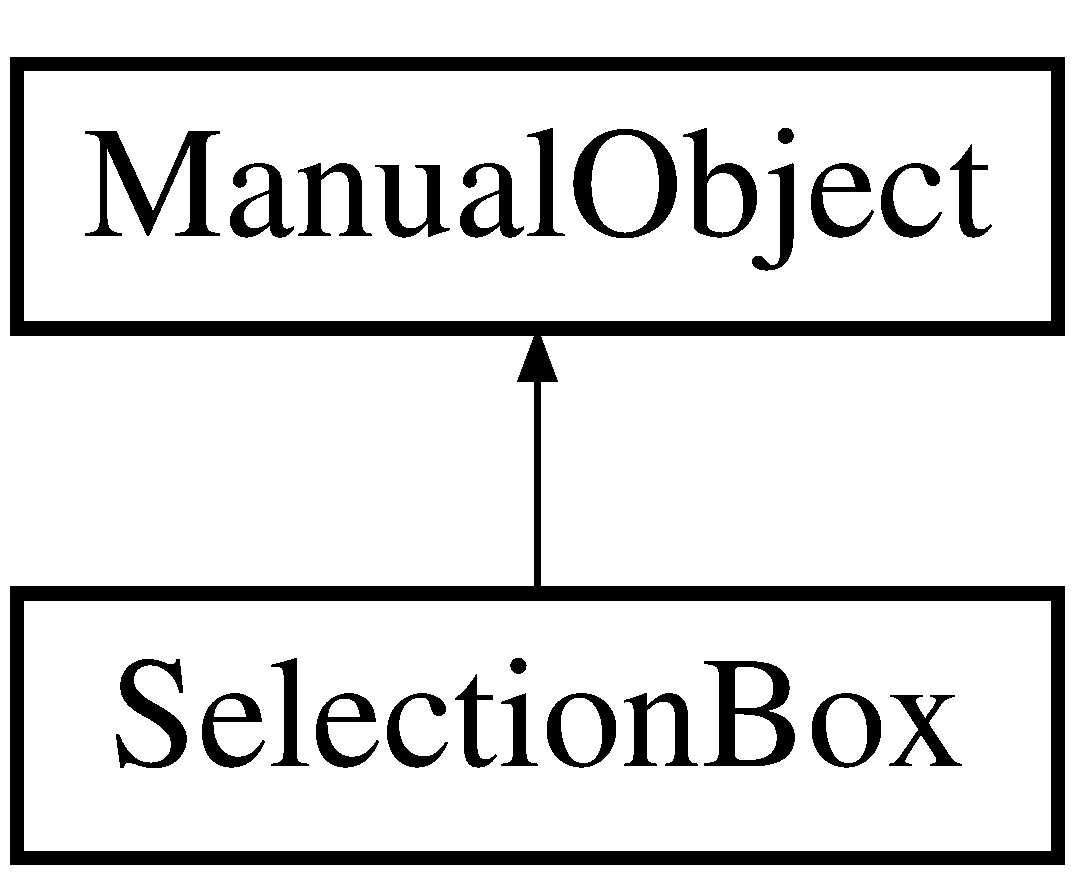
\includegraphics[height=2.000000cm]{class_selection_box}
\end{center}
\end{figure}
\subsection*{Public Member Functions}
\begin{DoxyCompactItemize}
\item 
\hyperlink{class_selection_box_a4f133c8badc39fb16a58188e7bd81399}{Selection\+Box} (const Ogre\+::\+String \&, \hyperlink{class_entity_system}{Entity\+System} \&, Ogre\+::\+Plane\+Bounded\+Volume\+List\+Scene\+Query \&, Ogre\+::\+Ray\+Scene\+Query \&, Ogre\+::\+Scene\+Manager \&)
\begin{DoxyCompactList}\small\item\em Constructor. \end{DoxyCompactList}\item 
\hyperlink{class_selection_box_ad7ca81556a52cdd7f21422331a845ef9}{$\sim$\+Selection\+Box} ()
\begin{DoxyCompactList}\small\item\em Destructor. \end{DoxyCompactList}\item 
void \hyperlink{class_selection_box_adcded0c1617213d702126920e117ba33}{set\+\_\+corners} (tdt\+::real, tdt\+::real, tdt\+::real, tdt\+::real)
\begin{DoxyCompactList}\small\item\em Recreates the selection box with the given coordinates. \end{DoxyCompactList}\item 
void \hyperlink{class_selection_box_ac8545c527a1fd5c28de1efd436765f5e}{set\+\_\+corners} (const Ogre\+::\+Vector2 \&, const Ogre\+::\+Vector2 \&)
\begin{DoxyCompactList}\small\item\em Overload of the Selection\+Box\+::set\+\_\+corners(float, float, float, float) method used as a simple interface when using vectors. \end{DoxyCompactList}\item 
std\+::vector$<$ tdt\+::uint $>$ \& \hyperlink{class_selection_box_a9f4c4958798dedb1cf97737e605408eb}{get\+\_\+selected\+\_\+entities} ()
\begin{DoxyCompactList}\small\item\em Returns (by reference) a vector containing ID\textquotesingle{}s of all currently selected entities. \end{DoxyCompactList}\item 
void \hyperlink{class_selection_box_a95cf76c371678c6f644f50577ee59c9f}{select\+\_\+object} (Ogre\+::\+Movable\+Object \&)
\begin{DoxyCompactList}\small\item\em Adds a given object to the vector of selected entities. \end{DoxyCompactList}\item 
void \hyperlink{class_selection_box_aae870741250f1247633a76d7343114e1}{clear\+\_\+selected\+\_\+entities} ()
\begin{DoxyCompactList}\small\item\em Deselects all currently selected entities. \end{DoxyCompactList}\item 
void \hyperlink{class_selection_box_a8013255ab23d92e60bb28378e837421a}{execute\+\_\+selection} (const Ogre\+::\+Vector2 \&, Ogre\+::\+Camera \&, bool=false)
\begin{DoxyCompactList}\small\item\em Performs the selection, to be called when the mouse is released. \end{DoxyCompactList}\item 
void \hyperlink{class_selection_box_aa9f4cbe292d3386e212495e8e31d5f40}{set\+\_\+starting\+\_\+point} (const Ogre\+::\+Vector2 \&)
\begin{DoxyCompactList}\small\item\em Sets the starting point of the current selection, should be called upon the initial mouse button click. \end{DoxyCompactList}\item 
void \hyperlink{class_selection_box_a135517752479cff0bb5bf32ed9b5277b}{set\+\_\+selecting} (bool)
\begin{DoxyCompactList}\small\item\em Sets the selecting mode (and the visibility flag of the selection box). \end{DoxyCompactList}\item 
bool \hyperlink{class_selection_box_ab8e28df20f6f27f40512cd32d7f9b047}{is\+\_\+selecting} () const 
\begin{DoxyCompactList}\small\item\em Returns true if the selection box is currently selecting. \end{DoxyCompactList}\item 
void \hyperlink{class_selection_box_a7bfb19cdb0c9c999784e1af6cd352fc8}{extend\+\_\+to} (const Ogre\+::\+Vector2 \&)
\begin{DoxyCompactList}\small\item\em Extends the selection box to a given coordinate, using the start\+\_\+ coordinate provided by \hyperlink{class_selection_box_aa9f4cbe292d3386e212495e8e31d5f40}{Selection\+Box\+::set\+\_\+starting\+\_\+point} as the initial point. \end{DoxyCompactList}\end{DoxyCompactItemize}
\subsection*{Private Member Functions}
\begin{DoxyCompactItemize}
\item 
void \hyperlink{class_selection_box_a46bb8a54b0f9549ce74985f528ff7c81}{execute\+\_\+single\+\_\+selection} (Ogre\+::\+Camera \&)
\begin{DoxyCompactList}\small\item\em Used within the \hyperlink{class_selection_box_a8013255ab23d92e60bb28378e837421a}{Selection\+Box\+::execute\+\_\+selection} method when the selection box is two small (i.\+e. \end{DoxyCompactList}\end{DoxyCompactItemize}
\subsection*{Private Attributes}
\begin{DoxyCompactItemize}
\item 
std\+::vector$<$ tdt\+::uint $>$ \hyperlink{class_selection_box_a47f43b49a4eeab82ac9c0423b689d8c7}{selected\+\_\+entities\+\_\+}
\begin{DoxyCompactList}\small\item\em Currently selected entities. \end{DoxyCompactList}\item 
\hyperlink{class_entity_system}{Entity\+System} \& \hyperlink{class_selection_box_ac0e69cb5092894d810d6084ab9daf305}{entities\+\_\+}
\begin{DoxyCompactList}\small\item\em Reference to the game\textquotesingle{}s entity system, used to identify an entity ID from an entity Scene\+Node. \end{DoxyCompactList}\item 
Ogre\+::\+Vector2 \hyperlink{class_selection_box_a972855bf908b9a6a5048b3fb842dc769}{start\+\_\+}
\begin{DoxyCompactList}\small\item\em Vector containing the coordinates of the starting point of the selection. \end{DoxyCompactList}\item 
Ogre\+::\+Plane\+Bounded\+Volume\+List\+Scene\+Query \& \hyperlink{class_selection_box_a2218879b200ef6b963ea834d38010831}{volume\+\_\+query\+\_\+}
\begin{DoxyCompactList}\small\item\em Scene query used to find all the entities that are within the selection box. \end{DoxyCompactList}\item 
Ogre\+::\+Ray\+Scene\+Query \& \hyperlink{class_selection_box_a3ff14222f216c6d97f2a1fd7da76f96a}{ray\+\_\+query\+\_\+}
\begin{DoxyCompactList}\small\item\em Scene query used to find an entity when the selection box is too small. \end{DoxyCompactList}\item 
bool \hyperlink{class_selection_box_ae814ae0409771480132a038d4082fe97}{selection\+\_\+in\+\_\+progress\+\_\+}
\begin{DoxyCompactList}\small\item\em Determines if the player is currently selecting entities. \end{DoxyCompactList}\item 
Ogre\+::\+Scene\+Manager \& \hyperlink{class_selection_box_a4b844958cbf4e43926e44508c62476af}{scene\+\_\+mgr\+\_\+}
\begin{DoxyCompactList}\small\item\em Reference to the game\textquotesingle{}s main scene manager. \end{DoxyCompactList}\end{DoxyCompactItemize}


\subsection{Detailed Description}
Class representing the ingame selection box (created by moving the left mouse while pressing the left mouse button) to select multiple entities on screen or a single entity (by simply clicking). 

Definition at line 13 of file Selection\+Box.\+hpp.



\subsection{Constructor \& Destructor Documentation}
\index{Selection\+Box@{Selection\+Box}!Selection\+Box@{Selection\+Box}}
\index{Selection\+Box@{Selection\+Box}!Selection\+Box@{Selection\+Box}}
\subsubsection[{\texorpdfstring{Selection\+Box(const Ogre\+::\+String \&, Entity\+System \&, Ogre\+::\+Plane\+Bounded\+Volume\+List\+Scene\+Query \&, Ogre\+::\+Ray\+Scene\+Query \&, Ogre\+::\+Scene\+Manager \&)}{SelectionBox(const Ogre::String &, EntitySystem &, Ogre::PlaneBoundedVolumeListSceneQuery &, Ogre::RaySceneQuery &, Ogre::SceneManager &)}}]{\setlength{\rightskip}{0pt plus 5cm}Selection\+Box\+::\+Selection\+Box (
\begin{DoxyParamCaption}
\item[{const Ogre\+::\+String \&}]{name, }
\item[{{\bf Entity\+System} \&}]{ents, }
\item[{Ogre\+::\+Plane\+Bounded\+Volume\+List\+Scene\+Query \&}]{vol\+\_\+query, }
\item[{Ogre\+::\+Ray\+Scene\+Query \&}]{ray\+\_\+query, }
\item[{Ogre\+::\+Scene\+Manager \&}]{mgr}
\end{DoxyParamCaption}
)}\hypertarget{class_selection_box_a4f133c8badc39fb16a58188e7bd81399}{}\label{class_selection_box_a4f133c8badc39fb16a58188e7bd81399}


Constructor. 


\begin{DoxyParams}{Parameters}
{\em Name} & of this object (passed to Manual\+Object constructor -\/ hence the type). \\
\hline
{\em Reference} & to a volume query used for multi selection. \\
\hline
{\em Reference} & to a ray query used for single selection. \\
\hline
{\em Reference} & to the game\textquotesingle{}s main scene manager. \\
\hline
\end{DoxyParams}


Definition at line 5 of file Selection\+Box.\+cpp.

\index{Selection\+Box@{Selection\+Box}!````~Selection\+Box@{$\sim$\+Selection\+Box}}
\index{````~Selection\+Box@{$\sim$\+Selection\+Box}!Selection\+Box@{Selection\+Box}}
\subsubsection[{\texorpdfstring{$\sim$\+Selection\+Box()}{~SelectionBox()}}]{\setlength{\rightskip}{0pt plus 5cm}Selection\+Box\+::$\sim$\+Selection\+Box (
\begin{DoxyParamCaption}
{}
\end{DoxyParamCaption}
)}\hypertarget{class_selection_box_ad7ca81556a52cdd7f21422331a845ef9}{}\label{class_selection_box_ad7ca81556a52cdd7f21422331a845ef9}


Destructor. 

\begin{DoxyNote}{Note}
Even thous the queries are captured by reference, they need to be destroyed manually using the scene manager. 
\end{DoxyNote}


Definition at line 19 of file Selection\+Box.\+cpp.



\subsection{Member Function Documentation}
\index{Selection\+Box@{Selection\+Box}!clear\+\_\+selected\+\_\+entities@{clear\+\_\+selected\+\_\+entities}}
\index{clear\+\_\+selected\+\_\+entities@{clear\+\_\+selected\+\_\+entities}!Selection\+Box@{Selection\+Box}}
\subsubsection[{\texorpdfstring{clear\+\_\+selected\+\_\+entities()}{clear_selected_entities()}}]{\setlength{\rightskip}{0pt plus 5cm}void Selection\+Box\+::clear\+\_\+selected\+\_\+entities (
\begin{DoxyParamCaption}
{}
\end{DoxyParamCaption}
)}\hypertarget{class_selection_box_aae870741250f1247633a76d7343114e1}{}\label{class_selection_box_aae870741250f1247633a76d7343114e1}


Deselects all currently selected entities. 



Definition at line 76 of file Selection\+Box.\+cpp.

\index{Selection\+Box@{Selection\+Box}!execute\+\_\+selection@{execute\+\_\+selection}}
\index{execute\+\_\+selection@{execute\+\_\+selection}!Selection\+Box@{Selection\+Box}}
\subsubsection[{\texorpdfstring{execute\+\_\+selection(const Ogre\+::\+Vector2 \&, Ogre\+::\+Camera \&, bool=false)}{execute_selection(const Ogre::Vector2 &, Ogre::Camera &, bool=false)}}]{\setlength{\rightskip}{0pt plus 5cm}void Selection\+Box\+::execute\+\_\+selection (
\begin{DoxyParamCaption}
\item[{const Ogre\+::\+Vector2 \&}]{end, }
\item[{Ogre\+::\+Camera \&}]{cam, }
\item[{bool}]{append = {\ttfamily false}}
\end{DoxyParamCaption}
)}\hypertarget{class_selection_box_a8013255ab23d92e60bb28378e837421a}{}\label{class_selection_box_a8013255ab23d92e60bb28378e837421a}


Performs the selection, to be called when the mouse is released. 


\begin{DoxyParams}{Parameters}
{\em Coordinate} & of the end point of the box (mouse position). \\
\hline
{\em Reference} & to the camera the query should be performed from. \\
\hline
{\em True} & if the the new selection should be appended to the current selection. \\
\hline
\end{DoxyParams}
\begin{DoxyNote}{Note}
The starting point has to be saved prior to this call (i.\+e. when the mouse button gets pressed) in order for the selection to work properly. 
\end{DoxyNote}


Definition at line 88 of file Selection\+Box.\+cpp.

\index{Selection\+Box@{Selection\+Box}!execute\+\_\+single\+\_\+selection@{execute\+\_\+single\+\_\+selection}}
\index{execute\+\_\+single\+\_\+selection@{execute\+\_\+single\+\_\+selection}!Selection\+Box@{Selection\+Box}}
\subsubsection[{\texorpdfstring{execute\+\_\+single\+\_\+selection(\+Ogre\+::\+Camera \&)}{execute_single_selection(Ogre::Camera &)}}]{\setlength{\rightskip}{0pt plus 5cm}void Selection\+Box\+::execute\+\_\+single\+\_\+selection (
\begin{DoxyParamCaption}
\item[{Ogre\+::\+Camera \&}]{cam}
\end{DoxyParamCaption}
)\hspace{0.3cm}{\ttfamily [private]}}\hypertarget{class_selection_box_a46bb8a54b0f9549ce74985f528ff7c81}{}\label{class_selection_box_a46bb8a54b0f9549ce74985f528ff7c81}


Used within the \hyperlink{class_selection_box_a8013255ab23d92e60bb28378e837421a}{Selection\+Box\+::execute\+\_\+selection} method when the selection box is two small (i.\+e. 

a single click) and performs a ray query selecting a single closest entity under the player\textquotesingle{}s cursor. 
\begin{DoxyParams}{Parameters}
{\em Reference} & to the game\textquotesingle{}s main camera. \\
\hline
\end{DoxyParams}


Definition at line 144 of file Selection\+Box.\+cpp.

\index{Selection\+Box@{Selection\+Box}!extend\+\_\+to@{extend\+\_\+to}}
\index{extend\+\_\+to@{extend\+\_\+to}!Selection\+Box@{Selection\+Box}}
\subsubsection[{\texorpdfstring{extend\+\_\+to(const Ogre\+::\+Vector2 \&)}{extend_to(const Ogre::Vector2 &)}}]{\setlength{\rightskip}{0pt plus 5cm}void Selection\+Box\+::extend\+\_\+to (
\begin{DoxyParamCaption}
\item[{const Ogre\+::\+Vector2 \&}]{end}
\end{DoxyParamCaption}
)}\hypertarget{class_selection_box_a7bfb19cdb0c9c999784e1af6cd352fc8}{}\label{class_selection_box_a7bfb19cdb0c9c999784e1af6cd352fc8}


Extends the selection box to a given coordinate, using the start\+\_\+ coordinate provided by \hyperlink{class_selection_box_aa9f4cbe292d3386e212495e8e31d5f40}{Selection\+Box\+::set\+\_\+starting\+\_\+point} as the initial point. 


\begin{DoxyParams}{Parameters}
{\em Coordinate} & of the ending point. \\
\hline
\end{DoxyParams}


Definition at line 139 of file Selection\+Box.\+cpp.

\index{Selection\+Box@{Selection\+Box}!get\+\_\+selected\+\_\+entities@{get\+\_\+selected\+\_\+entities}}
\index{get\+\_\+selected\+\_\+entities@{get\+\_\+selected\+\_\+entities}!Selection\+Box@{Selection\+Box}}
\subsubsection[{\texorpdfstring{get\+\_\+selected\+\_\+entities()}{get_selected_entities()}}]{\setlength{\rightskip}{0pt plus 5cm}std\+::vector$<$ tdt\+::uint $>$ \& Selection\+Box\+::get\+\_\+selected\+\_\+entities (
\begin{DoxyParamCaption}
{}
\end{DoxyParamCaption}
)}\hypertarget{class_selection_box_a9f4c4958798dedb1cf97737e605408eb}{}\label{class_selection_box_a9f4c4958798dedb1cf97737e605408eb}


Returns (by reference) a vector containing ID\textquotesingle{}s of all currently selected entities. 



Definition at line 57 of file Selection\+Box.\+cpp.

\index{Selection\+Box@{Selection\+Box}!is\+\_\+selecting@{is\+\_\+selecting}}
\index{is\+\_\+selecting@{is\+\_\+selecting}!Selection\+Box@{Selection\+Box}}
\subsubsection[{\texorpdfstring{is\+\_\+selecting() const }{is_selecting() const }}]{\setlength{\rightskip}{0pt plus 5cm}bool Selection\+Box\+::is\+\_\+selecting (
\begin{DoxyParamCaption}
{}
\end{DoxyParamCaption}
) const}\hypertarget{class_selection_box_ab8e28df20f6f27f40512cd32d7f9b047}{}\label{class_selection_box_ab8e28df20f6f27f40512cd32d7f9b047}


Returns true if the selection box is currently selecting. 



Definition at line 134 of file Selection\+Box.\+cpp.

\index{Selection\+Box@{Selection\+Box}!select\+\_\+object@{select\+\_\+object}}
\index{select\+\_\+object@{select\+\_\+object}!Selection\+Box@{Selection\+Box}}
\subsubsection[{\texorpdfstring{select\+\_\+object(\+Ogre\+::\+Movable\+Object \&)}{select_object(Ogre::MovableObject &)}}]{\setlength{\rightskip}{0pt plus 5cm}void Selection\+Box\+::select\+\_\+object (
\begin{DoxyParamCaption}
\item[{Ogre\+::\+Movable\+Object \&}]{obj}
\end{DoxyParamCaption}
)}\hypertarget{class_selection_box_a95cf76c371678c6f644f50577ee59c9f}{}\label{class_selection_box_a95cf76c371678c6f644f50577ee59c9f}


Adds a given object to the vector of selected entities. 


\begin{DoxyParams}{Parameters}
{\em Reference} & to the object from which the entity ID will be deduced. \\
\hline
\end{DoxyParams}


Definition at line 62 of file Selection\+Box.\+cpp.

\index{Selection\+Box@{Selection\+Box}!set\+\_\+corners@{set\+\_\+corners}}
\index{set\+\_\+corners@{set\+\_\+corners}!Selection\+Box@{Selection\+Box}}
\subsubsection[{\texorpdfstring{set\+\_\+corners(tdt\+::real, tdt\+::real, tdt\+::real, tdt\+::real)}{set_corners(tdt::real, tdt::real, tdt::real, tdt::real)}}]{\setlength{\rightskip}{0pt plus 5cm}void Selection\+Box\+::set\+\_\+corners (
\begin{DoxyParamCaption}
\item[{tdt\+::real}]{left, }
\item[{tdt\+::real}]{top, }
\item[{tdt\+::real}]{right, }
\item[{tdt\+::real}]{bott}
\end{DoxyParamCaption}
)}\hypertarget{class_selection_box_adcded0c1617213d702126920e117ba33}{}\label{class_selection_box_adcded0c1617213d702126920e117ba33}


Recreates the selection box with the given coordinates. 


\begin{DoxyParams}{Parameters}
{\em Left} & side coordinate. \\
\hline
{\em Top} & side coordinate. \\
\hline
{\em Right} & side coordinate. \\
\hline
{\em Bottom} & axis coordinate. \\
\hline
\end{DoxyParams}
Neccessary translation, mouse positions are normalized to belong to the (0,1) range, but the Ogre\+::\+Manual\+Object creation requires them to belong to the (-\/1, 1).

Definition at line 25 of file Selection\+Box.\+cpp.

\index{Selection\+Box@{Selection\+Box}!set\+\_\+corners@{set\+\_\+corners}}
\index{set\+\_\+corners@{set\+\_\+corners}!Selection\+Box@{Selection\+Box}}
\subsubsection[{\texorpdfstring{set\+\_\+corners(const Ogre\+::\+Vector2 \&, const Ogre\+::\+Vector2 \&)}{set_corners(const Ogre::Vector2 &, const Ogre::Vector2 &)}}]{\setlength{\rightskip}{0pt plus 5cm}void Selection\+Box\+::set\+\_\+corners (
\begin{DoxyParamCaption}
\item[{const Ogre\+::\+Vector2 \&}]{t\+\_\+l, }
\item[{const Ogre\+::\+Vector2 \&}]{b\+\_\+r}
\end{DoxyParamCaption}
)}\hypertarget{class_selection_box_ac8545c527a1fd5c28de1efd436765f5e}{}\label{class_selection_box_ac8545c527a1fd5c28de1efd436765f5e}


Overload of the Selection\+Box\+::set\+\_\+corners(float, float, float, float) method used as a simple interface when using vectors. 


\begin{DoxyParams}{Parameters}
{\em Coordinate} & of the top left corner. \\
\hline
{\em Coordinate} & of the bottom right corner. \\
\hline
\end{DoxyParams}


Definition at line 50 of file Selection\+Box.\+cpp.

\index{Selection\+Box@{Selection\+Box}!set\+\_\+selecting@{set\+\_\+selecting}}
\index{set\+\_\+selecting@{set\+\_\+selecting}!Selection\+Box@{Selection\+Box}}
\subsubsection[{\texorpdfstring{set\+\_\+selecting(bool)}{set_selecting(bool)}}]{\setlength{\rightskip}{0pt plus 5cm}void Selection\+Box\+::set\+\_\+selecting (
\begin{DoxyParamCaption}
\item[{bool}]{sel}
\end{DoxyParamCaption}
)}\hypertarget{class_selection_box_a135517752479cff0bb5bf32ed9b5277b}{}\label{class_selection_box_a135517752479cff0bb5bf32ed9b5277b}


Sets the selecting mode (and the visibility flag of the selection box). 


\begin{DoxyParams}{Parameters}
{\em Bool} & value representing the new visibility mode. \\
\hline
\end{DoxyParams}


Definition at line 128 of file Selection\+Box.\+cpp.

\index{Selection\+Box@{Selection\+Box}!set\+\_\+starting\+\_\+point@{set\+\_\+starting\+\_\+point}}
\index{set\+\_\+starting\+\_\+point@{set\+\_\+starting\+\_\+point}!Selection\+Box@{Selection\+Box}}
\subsubsection[{\texorpdfstring{set\+\_\+starting\+\_\+point(const Ogre\+::\+Vector2 \&)}{set_starting_point(const Ogre::Vector2 &)}}]{\setlength{\rightskip}{0pt plus 5cm}void Selection\+Box\+::set\+\_\+starting\+\_\+point (
\begin{DoxyParamCaption}
\item[{const Ogre\+::\+Vector2 \&}]{start}
\end{DoxyParamCaption}
)}\hypertarget{class_selection_box_aa9f4cbe292d3386e212495e8e31d5f40}{}\label{class_selection_box_aa9f4cbe292d3386e212495e8e31d5f40}


Sets the starting point of the current selection, should be called upon the initial mouse button click. 


\begin{DoxyParams}{Parameters}
{\em Coordinate} & of the starting point. \\
\hline
\end{DoxyParams}


Definition at line 123 of file Selection\+Box.\+cpp.



\subsection{Member Data Documentation}
\index{Selection\+Box@{Selection\+Box}!entities\+\_\+@{entities\+\_\+}}
\index{entities\+\_\+@{entities\+\_\+}!Selection\+Box@{Selection\+Box}}
\subsubsection[{\texorpdfstring{entities\+\_\+}{entities_}}]{\setlength{\rightskip}{0pt plus 5cm}{\bf Entity\+System}\& Selection\+Box\+::entities\+\_\+\hspace{0.3cm}{\ttfamily [private]}}\hypertarget{class_selection_box_ac0e69cb5092894d810d6084ab9daf305}{}\label{class_selection_box_ac0e69cb5092894d810d6084ab9daf305}


Reference to the game\textquotesingle{}s entity system, used to identify an entity ID from an entity Scene\+Node. 



Definition at line 120 of file Selection\+Box.\+hpp.

\index{Selection\+Box@{Selection\+Box}!ray\+\_\+query\+\_\+@{ray\+\_\+query\+\_\+}}
\index{ray\+\_\+query\+\_\+@{ray\+\_\+query\+\_\+}!Selection\+Box@{Selection\+Box}}
\subsubsection[{\texorpdfstring{ray\+\_\+query\+\_\+}{ray_query_}}]{\setlength{\rightskip}{0pt plus 5cm}Ogre\+::\+Ray\+Scene\+Query\& Selection\+Box\+::ray\+\_\+query\+\_\+\hspace{0.3cm}{\ttfamily [private]}}\hypertarget{class_selection_box_a3ff14222f216c6d97f2a1fd7da76f96a}{}\label{class_selection_box_a3ff14222f216c6d97f2a1fd7da76f96a}


Scene query used to find an entity when the selection box is too small. 



Definition at line 136 of file Selection\+Box.\+hpp.

\index{Selection\+Box@{Selection\+Box}!scene\+\_\+mgr\+\_\+@{scene\+\_\+mgr\+\_\+}}
\index{scene\+\_\+mgr\+\_\+@{scene\+\_\+mgr\+\_\+}!Selection\+Box@{Selection\+Box}}
\subsubsection[{\texorpdfstring{scene\+\_\+mgr\+\_\+}{scene_mgr_}}]{\setlength{\rightskip}{0pt plus 5cm}Ogre\+::\+Scene\+Manager\& Selection\+Box\+::scene\+\_\+mgr\+\_\+\hspace{0.3cm}{\ttfamily [private]}}\hypertarget{class_selection_box_a4b844958cbf4e43926e44508c62476af}{}\label{class_selection_box_a4b844958cbf4e43926e44508c62476af}


Reference to the game\textquotesingle{}s main scene manager. 



Definition at line 146 of file Selection\+Box.\+hpp.

\index{Selection\+Box@{Selection\+Box}!selected\+\_\+entities\+\_\+@{selected\+\_\+entities\+\_\+}}
\index{selected\+\_\+entities\+\_\+@{selected\+\_\+entities\+\_\+}!Selection\+Box@{Selection\+Box}}
\subsubsection[{\texorpdfstring{selected\+\_\+entities\+\_\+}{selected_entities_}}]{\setlength{\rightskip}{0pt plus 5cm}std\+::vector$<$tdt\+::uint$>$ Selection\+Box\+::selected\+\_\+entities\+\_\+\hspace{0.3cm}{\ttfamily [private]}}\hypertarget{class_selection_box_a47f43b49a4eeab82ac9c0423b689d8c7}{}\label{class_selection_box_a47f43b49a4eeab82ac9c0423b689d8c7}


Currently selected entities. 



Definition at line 114 of file Selection\+Box.\+hpp.

\index{Selection\+Box@{Selection\+Box}!selection\+\_\+in\+\_\+progress\+\_\+@{selection\+\_\+in\+\_\+progress\+\_\+}}
\index{selection\+\_\+in\+\_\+progress\+\_\+@{selection\+\_\+in\+\_\+progress\+\_\+}!Selection\+Box@{Selection\+Box}}
\subsubsection[{\texorpdfstring{selection\+\_\+in\+\_\+progress\+\_\+}{selection_in_progress_}}]{\setlength{\rightskip}{0pt plus 5cm}bool Selection\+Box\+::selection\+\_\+in\+\_\+progress\+\_\+\hspace{0.3cm}{\ttfamily [private]}}\hypertarget{class_selection_box_ae814ae0409771480132a038d4082fe97}{}\label{class_selection_box_ae814ae0409771480132a038d4082fe97}


Determines if the player is currently selecting entities. 



Definition at line 141 of file Selection\+Box.\+hpp.

\index{Selection\+Box@{Selection\+Box}!start\+\_\+@{start\+\_\+}}
\index{start\+\_\+@{start\+\_\+}!Selection\+Box@{Selection\+Box}}
\subsubsection[{\texorpdfstring{start\+\_\+}{start_}}]{\setlength{\rightskip}{0pt plus 5cm}Ogre\+::\+Vector2 Selection\+Box\+::start\+\_\+\hspace{0.3cm}{\ttfamily [private]}}\hypertarget{class_selection_box_a972855bf908b9a6a5048b3fb842dc769}{}\label{class_selection_box_a972855bf908b9a6a5048b3fb842dc769}


Vector containing the coordinates of the starting point of the selection. 

(Ending point will be specified in the \hyperlink{class_selection_box_a8013255ab23d92e60bb28378e837421a}{Selection\+Box\+::execute\+\_\+selection} method.) 

Definition at line 126 of file Selection\+Box.\+hpp.

\index{Selection\+Box@{Selection\+Box}!volume\+\_\+query\+\_\+@{volume\+\_\+query\+\_\+}}
\index{volume\+\_\+query\+\_\+@{volume\+\_\+query\+\_\+}!Selection\+Box@{Selection\+Box}}
\subsubsection[{\texorpdfstring{volume\+\_\+query\+\_\+}{volume_query_}}]{\setlength{\rightskip}{0pt plus 5cm}Ogre\+::\+Plane\+Bounded\+Volume\+List\+Scene\+Query\& Selection\+Box\+::volume\+\_\+query\+\_\+\hspace{0.3cm}{\ttfamily [private]}}\hypertarget{class_selection_box_a2218879b200ef6b963ea834d38010831}{}\label{class_selection_box_a2218879b200ef6b963ea834d38010831}


Scene query used to find all the entities that are within the selection box. 



Definition at line 131 of file Selection\+Box.\+hpp.



The documentation for this class was generated from the following files\+:\begin{DoxyCompactItemize}
\item 
tools/Selection\+Box.\+hpp\item 
tools/Selection\+Box.\+cpp\end{DoxyCompactItemize}

\hypertarget{struct_spellcaster_1_1_s_p_e_l_l}{}\section{Spellcaster\+:\+:S\+P\+E\+LL Struct Reference}
\label{struct_spellcaster_1_1_s_p_e_l_l}\index{Spellcaster\+::\+S\+P\+E\+LL@{Spellcaster\+::\+S\+P\+E\+LL}}


A structure representing a spell by containing it\textquotesingle{}s type and name.  


\subsection*{Public Attributes}
\begin{DoxyCompactItemize}
\item 
S\+P\+E\+L\+L\+\_\+\+T\+Y\+PE {\bfseries type\+\_\+}\hypertarget{struct_spellcaster_1_1_s_p_e_l_l_ad313aa994f76d1a79ab488bdfb9cfb40}{}\label{struct_spellcaster_1_1_s_p_e_l_l_ad313aa994f76d1a79ab488bdfb9cfb40}

\item 
std\+::string {\bfseries spell\+\_\+}\hypertarget{struct_spellcaster_1_1_s_p_e_l_l_a5400b8662abb37ffc648278bb5b07b93}{}\label{struct_spellcaster_1_1_s_p_e_l_l_a5400b8662abb37ffc648278bb5b07b93}

\end{DoxyCompactItemize}


\subsection{Detailed Description}
A structure representing a spell by containing it\textquotesingle{}s type and name. 

Definition at line 102 of file Spellcaster.\+hpp.



The documentation for this struct was generated from the following file\+:\begin{DoxyCompactItemize}
\item 
tools/Spellcaster.\+hpp\end{DoxyCompactItemize}

\hypertarget{class_spellcaster}{}\section{Spellcaster Class Reference}
\label{class_spellcaster}\index{Spellcaster@{Spellcaster}}


A utility class that manages the player\textquotesingle{}s spell casting and is usually called from input handlers and the spell casting window.  




{\ttfamily \#include $<$Spellcaster.\+hpp$>$}

\subsection*{Classes}
\begin{DoxyCompactItemize}
\item 
struct \hyperlink{struct_spellcaster_1_1_s_p_e_l_l}{S\+P\+E\+LL}
\begin{DoxyCompactList}\small\item\em A structure representing a spell by containing it\textquotesingle{}s type and name. \end{DoxyCompactList}\end{DoxyCompactItemize}
\subsection*{Public Member Functions}
\begin{DoxyCompactItemize}
\item 
\hyperlink{class_spellcaster_a633d55dbde7a54a2142064ae68865a51}{Spellcaster} (\hyperlink{class_entity_placer}{Entity\+Placer} \&, \hyperlink{class_selection_box}{Selection\+Box} \&)
\begin{DoxyCompactList}\small\item\em Constructor. \end{DoxyCompactList}\item 
\hyperlink{class_spellcaster_ac4ec32a60b9e23f653f59fa0f1ee6716}{$\sim$\+Spellcaster} ()=default
\begin{DoxyCompactList}\small\item\em Destructor. \end{DoxyCompactList}\item 
void \hyperlink{class_spellcaster_ab0b5ede64fc2de3e6cfc2c27ac1c2524}{set\+\_\+spell\+\_\+type} (S\+P\+E\+L\+L\+\_\+\+T\+Y\+PE)
\begin{DoxyCompactList}\small\item\em Sets the type of the currently casted spell. \end{DoxyCompactList}\item 
S\+P\+E\+L\+L\+\_\+\+T\+Y\+PE \hyperlink{class_spellcaster_a988a60b96ba7ecfd99e8c462cc446224}{get\+\_\+spell\+\_\+type} () const 
\begin{DoxyCompactList}\small\item\em Returns the type of the currently casted spell. \end{DoxyCompactList}\item 
void \hyperlink{class_spellcaster_a4d4747d2b5d28699ff49f9e73ab674ef}{set\+\_\+spell} (const std\+::string \&)
\begin{DoxyCompactList}\small\item\em Sets the name of the currently casted spell. \end{DoxyCompactList}\item 
const std\+::string \& \hyperlink{class_spellcaster_a1ea142cee9e86569f1e0dfd6ae09a291}{get\+\_\+spell} () const 
\begin{DoxyCompactList}\small\item\em Returns the name of the currently casted spell. \end{DoxyCompactList}\item 
void \hyperlink{class_spellcaster_a602c7b78f2c8a512002422624b651c1d}{cast} (Ogre\+::\+Vector2=Ogre\+::\+Vector2\{\})
\begin{DoxyCompactList}\small\item\em Applies the effect of the currently casted spell. \end{DoxyCompactList}\item 
S\+P\+E\+L\+L\+\_\+\+T\+Y\+PE \hyperlink{class_spellcaster_a6a7435cd3d8af819a0b1f736ef7d491a}{get\+\_\+last\+\_\+spell\+\_\+type} () const 
\begin{DoxyCompactList}\small\item\em Returns the type of the previously casted spell. \end{DoxyCompactList}\item 
const std\+::string \& \hyperlink{class_spellcaster_a303e54a79abbf32acce747440600f573}{get\+\_\+last\+\_\+spell} () const 
\begin{DoxyCompactList}\small\item\em Returns the name of the previously casted spell. \end{DoxyCompactList}\item 
void \hyperlink{class_spellcaster_aea41ed591b51c20d0b3ffc2b4a360a40}{set\+\_\+last\+\_\+spell\+\_\+id} (tdt\+::uint)
\begin{DoxyCompactList}\small\item\em Sets the ID of the entity created by the last spell. \end{DoxyCompactList}\item 
tdt\+::uint \hyperlink{class_spellcaster_ab92d160481f58d7a2eb68332a436a198}{get\+\_\+last\+\_\+spell\+\_\+id} () const 
\begin{DoxyCompactList}\small\item\em Returns the ID of the entity created by the last spell. \end{DoxyCompactList}\item 
bool \hyperlink{class_spellcaster_a7387c8b8df16eaec70d2b75d2a5ad0f8}{is\+\_\+casting} () const 
\begin{DoxyCompactList}\small\item\em Returns true if this spellcaster is currently casting, false otherwise. \end{DoxyCompactList}\item 
void \hyperlink{class_spellcaster_ae836e98789e2f320d1f8f3aa2df5ca0e}{stop\+\_\+casting} ()
\begin{DoxyCompactList}\small\item\em Immediately stops any cast being performed. \end{DoxyCompactList}\end{DoxyCompactItemize}
\subsection*{Private Attributes}
\begin{DoxyCompactItemize}
\item 
\hyperlink{class_entity_placer}{Entity\+Placer} \& \hyperlink{class_spellcaster_afc71d4b4359263bbe6b5097ffdf2213d}{placer\+\_\+}
\begin{DoxyCompactList}\small\item\em Used to place entities created by placing spell. \end{DoxyCompactList}\item 
\hyperlink{class_selection_box}{Selection\+Box} \& \hyperlink{class_spellcaster_af3aeccdb061ff26b308d3147d1fb8e4f}{selector\+\_\+}
\begin{DoxyCompactList}\small\item\em Used to get selected targets for targeted spells. \end{DoxyCompactList}\item 
\hyperlink{classlpp_1_1_script}{lpp\+::\+Script} \& \hyperlink{class_spellcaster_a7eb799aff1aff16e7eb5c319eaf1bb1c}{script\+\_\+}
\begin{DoxyCompactList}\small\item\em Reference to the scripting engine used for easier calls to the spell functions. \end{DoxyCompactList}\item 
\hyperlink{struct_spellcaster_1_1_s_p_e_l_l}{S\+P\+E\+LL} \hyperlink{class_spellcaster_a976dd2761e2db139d150e8b90283a89f}{curr\+\_\+spell\+\_\+}
\begin{DoxyCompactList}\small\item\em The spell that is currently being casted. \end{DoxyCompactList}\item 
\hyperlink{struct_spellcaster_1_1_s_p_e_l_l}{S\+P\+E\+LL} \hyperlink{class_spellcaster_a397320efd8c657b8e47694124ba45fd1}{last\+\_\+spell\+\_\+}
\begin{DoxyCompactList}\small\item\em The spell that has been casted previously. \end{DoxyCompactList}\item 
tdt\+::uint \hyperlink{class_spellcaster_a396c7fb9dfcf6d20086f47944e637e6f}{last\+\_\+spell\+\_\+id\+\_\+}
\begin{DoxyCompactList}\small\item\em ID of the entity created by a placing spell (if any). \end{DoxyCompactList}\end{DoxyCompactItemize}


\subsection{Detailed Description}
A utility class that manages the player\textquotesingle{}s spell casting and is usually called from input handlers and the spell casting window. 

Definition at line 18 of file Spellcaster.\+hpp.



\subsection{Constructor \& Destructor Documentation}
\index{Spellcaster@{Spellcaster}!Spellcaster@{Spellcaster}}
\index{Spellcaster@{Spellcaster}!Spellcaster@{Spellcaster}}
\subsubsection[{\texorpdfstring{Spellcaster(\+Entity\+Placer \&, Selection\+Box \&)}{Spellcaster(EntityPlacer &, SelectionBox &)}}]{\setlength{\rightskip}{0pt plus 5cm}Spellcaster\+::\+Spellcaster (
\begin{DoxyParamCaption}
\item[{{\bf Entity\+Placer} \&}]{placer, }
\item[{{\bf Selection\+Box} \&}]{selector}
\end{DoxyParamCaption}
)}\hypertarget{class_spellcaster_a633d55dbde7a54a2142064ae68865a51}{}\label{class_spellcaster_a633d55dbde7a54a2142064ae68865a51}


Constructor. 


\begin{DoxyParams}{Parameters}
{\em The} & placer that is used for placing spells. \\
\hline
{\em Selector} & that is used for targeted spells. \\
\hline
\end{DoxyParams}


Definition at line 8 of file Spellcaster.\+cpp.

\index{Spellcaster@{Spellcaster}!````~Spellcaster@{$\sim$\+Spellcaster}}
\index{````~Spellcaster@{$\sim$\+Spellcaster}!Spellcaster@{Spellcaster}}
\subsubsection[{\texorpdfstring{$\sim$\+Spellcaster()=default}{~Spellcaster()=default}}]{\setlength{\rightskip}{0pt plus 5cm}Spellcaster\+::$\sim$\+Spellcaster (
\begin{DoxyParamCaption}
{}
\end{DoxyParamCaption}
)\hspace{0.3cm}{\ttfamily [default]}}\hypertarget{class_spellcaster_ac4ec32a60b9e23f653f59fa0f1ee6716}{}\label{class_spellcaster_ac4ec32a60b9e23f653f59fa0f1ee6716}


Destructor. 



\subsection{Member Function Documentation}
\index{Spellcaster@{Spellcaster}!cast@{cast}}
\index{cast@{cast}!Spellcaster@{Spellcaster}}
\subsubsection[{\texorpdfstring{cast(\+Ogre\+::\+Vector2=\+Ogre\+::\+Vector2\lcurly{}\rcurly{})}{cast(Ogre::Vector2=Ogre::Vector2\{\})}}]{\setlength{\rightskip}{0pt plus 5cm}void Spellcaster\+::cast (
\begin{DoxyParamCaption}
\item[{Ogre\+::\+Vector2}]{mouse\+\_\+position = {\ttfamily Ogre\+:\+:Vector2\{\}}}
\end{DoxyParamCaption}
)}\hypertarget{class_spellcaster_a602c7b78f2c8a512002422624b651c1d}{}\label{class_spellcaster_a602c7b78f2c8a512002422624b651c1d}


Applies the effect of the currently casted spell. 


\begin{DoxyParams}{Parameters}
{\em Optional} & mouse position parameter for positional spells. \\
\hline
\end{DoxyParams}


Definition at line 36 of file Spellcaster.\+cpp.

\index{Spellcaster@{Spellcaster}!get\+\_\+last\+\_\+spell@{get\+\_\+last\+\_\+spell}}
\index{get\+\_\+last\+\_\+spell@{get\+\_\+last\+\_\+spell}!Spellcaster@{Spellcaster}}
\subsubsection[{\texorpdfstring{get\+\_\+last\+\_\+spell() const }{get_last_spell() const }}]{\setlength{\rightskip}{0pt plus 5cm}const std\+::string \& Spellcaster\+::get\+\_\+last\+\_\+spell (
\begin{DoxyParamCaption}
{}
\end{DoxyParamCaption}
) const}\hypertarget{class_spellcaster_a303e54a79abbf32acce747440600f573}{}\label{class_spellcaster_a303e54a79abbf32acce747440600f573}


Returns the name of the previously casted spell. 

(Used if spells have sequential effect -\/ like portals.) 

Definition at line 83 of file Spellcaster.\+cpp.

\index{Spellcaster@{Spellcaster}!get\+\_\+last\+\_\+spell\+\_\+id@{get\+\_\+last\+\_\+spell\+\_\+id}}
\index{get\+\_\+last\+\_\+spell\+\_\+id@{get\+\_\+last\+\_\+spell\+\_\+id}!Spellcaster@{Spellcaster}}
\subsubsection[{\texorpdfstring{get\+\_\+last\+\_\+spell\+\_\+id() const }{get_last_spell_id() const }}]{\setlength{\rightskip}{0pt plus 5cm}tdt\+::uint Spellcaster\+::get\+\_\+last\+\_\+spell\+\_\+id (
\begin{DoxyParamCaption}
{}
\end{DoxyParamCaption}
) const}\hypertarget{class_spellcaster_ab92d160481f58d7a2eb68332a436a198}{}\label{class_spellcaster_ab92d160481f58d7a2eb68332a436a198}


Returns the ID of the entity created by the last spell. 

(Used if spells have sequential effect -\/ like portals.) 

Definition at line 93 of file Spellcaster.\+cpp.

\index{Spellcaster@{Spellcaster}!get\+\_\+last\+\_\+spell\+\_\+type@{get\+\_\+last\+\_\+spell\+\_\+type}}
\index{get\+\_\+last\+\_\+spell\+\_\+type@{get\+\_\+last\+\_\+spell\+\_\+type}!Spellcaster@{Spellcaster}}
\subsubsection[{\texorpdfstring{get\+\_\+last\+\_\+spell\+\_\+type() const }{get_last_spell_type() const }}]{\setlength{\rightskip}{0pt plus 5cm}S\+P\+E\+L\+L\+\_\+\+T\+Y\+PE Spellcaster\+::get\+\_\+last\+\_\+spell\+\_\+type (
\begin{DoxyParamCaption}
{}
\end{DoxyParamCaption}
) const}\hypertarget{class_spellcaster_a6a7435cd3d8af819a0b1f736ef7d491a}{}\label{class_spellcaster_a6a7435cd3d8af819a0b1f736ef7d491a}


Returns the type of the previously casted spell. 

(Used if spells have sequential effect -\/ like portals.) 

Definition at line 78 of file Spellcaster.\+cpp.

\index{Spellcaster@{Spellcaster}!get\+\_\+spell@{get\+\_\+spell}}
\index{get\+\_\+spell@{get\+\_\+spell}!Spellcaster@{Spellcaster}}
\subsubsection[{\texorpdfstring{get\+\_\+spell() const }{get_spell() const }}]{\setlength{\rightskip}{0pt plus 5cm}const std\+::string \& Spellcaster\+::get\+\_\+spell (
\begin{DoxyParamCaption}
{}
\end{DoxyParamCaption}
) const}\hypertarget{class_spellcaster_a1ea142cee9e86569f1e0dfd6ae09a291}{}\label{class_spellcaster_a1ea142cee9e86569f1e0dfd6ae09a291}


Returns the name of the currently casted spell. 



Definition at line 31 of file Spellcaster.\+cpp.

\index{Spellcaster@{Spellcaster}!get\+\_\+spell\+\_\+type@{get\+\_\+spell\+\_\+type}}
\index{get\+\_\+spell\+\_\+type@{get\+\_\+spell\+\_\+type}!Spellcaster@{Spellcaster}}
\subsubsection[{\texorpdfstring{get\+\_\+spell\+\_\+type() const }{get_spell_type() const }}]{\setlength{\rightskip}{0pt plus 5cm}S\+P\+E\+L\+L\+\_\+\+T\+Y\+PE Spellcaster\+::get\+\_\+spell\+\_\+type (
\begin{DoxyParamCaption}
{}
\end{DoxyParamCaption}
) const}\hypertarget{class_spellcaster_a988a60b96ba7ecfd99e8c462cc446224}{}\label{class_spellcaster_a988a60b96ba7ecfd99e8c462cc446224}


Returns the type of the currently casted spell. 



Definition at line 20 of file Spellcaster.\+cpp.

\index{Spellcaster@{Spellcaster}!is\+\_\+casting@{is\+\_\+casting}}
\index{is\+\_\+casting@{is\+\_\+casting}!Spellcaster@{Spellcaster}}
\subsubsection[{\texorpdfstring{is\+\_\+casting() const }{is_casting() const }}]{\setlength{\rightskip}{0pt plus 5cm}bool Spellcaster\+::is\+\_\+casting (
\begin{DoxyParamCaption}
{}
\end{DoxyParamCaption}
) const}\hypertarget{class_spellcaster_a7387c8b8df16eaec70d2b75d2a5ad0f8}{}\label{class_spellcaster_a7387c8b8df16eaec70d2b75d2a5ad0f8}


Returns true if this spellcaster is currently casting, false otherwise. 



Definition at line 98 of file Spellcaster.\+cpp.

\index{Spellcaster@{Spellcaster}!set\+\_\+last\+\_\+spell\+\_\+id@{set\+\_\+last\+\_\+spell\+\_\+id}}
\index{set\+\_\+last\+\_\+spell\+\_\+id@{set\+\_\+last\+\_\+spell\+\_\+id}!Spellcaster@{Spellcaster}}
\subsubsection[{\texorpdfstring{set\+\_\+last\+\_\+spell\+\_\+id(tdt\+::uint)}{set_last_spell_id(tdt::uint)}}]{\setlength{\rightskip}{0pt plus 5cm}void Spellcaster\+::set\+\_\+last\+\_\+spell\+\_\+id (
\begin{DoxyParamCaption}
\item[{tdt\+::uint}]{val}
\end{DoxyParamCaption}
)}\hypertarget{class_spellcaster_aea41ed591b51c20d0b3ffc2b4a360a40}{}\label{class_spellcaster_aea41ed591b51c20d0b3ffc2b4a360a40}


Sets the ID of the entity created by the last spell. 

(Used if spells have sequential effect -\/ like portals.) 
\begin{DoxyParams}{Parameters}
{\em The} & ID of the entity created. \\
\hline
\end{DoxyParams}


Definition at line 88 of file Spellcaster.\+cpp.

\index{Spellcaster@{Spellcaster}!set\+\_\+spell@{set\+\_\+spell}}
\index{set\+\_\+spell@{set\+\_\+spell}!Spellcaster@{Spellcaster}}
\subsubsection[{\texorpdfstring{set\+\_\+spell(const std\+::string \&)}{set_spell(const std::string &)}}]{\setlength{\rightskip}{0pt plus 5cm}void Spellcaster\+::set\+\_\+spell (
\begin{DoxyParamCaption}
\item[{const std\+::string \&}]{val}
\end{DoxyParamCaption}
)}\hypertarget{class_spellcaster_a4d4747d2b5d28699ff49f9e73ab674ef}{}\label{class_spellcaster_a4d4747d2b5d28699ff49f9e73ab674ef}


Sets the name of the currently casted spell. 


\begin{DoxyParams}{Parameters}
{\em The} & new name. \\
\hline
\end{DoxyParams}


Definition at line 25 of file Spellcaster.\+cpp.

\index{Spellcaster@{Spellcaster}!set\+\_\+spell\+\_\+type@{set\+\_\+spell\+\_\+type}}
\index{set\+\_\+spell\+\_\+type@{set\+\_\+spell\+\_\+type}!Spellcaster@{Spellcaster}}
\subsubsection[{\texorpdfstring{set\+\_\+spell\+\_\+type(\+S\+P\+E\+L\+L\+\_\+\+T\+Y\+P\+E)}{set_spell_type(SPELL_TYPE)}}]{\setlength{\rightskip}{0pt plus 5cm}void Spellcaster\+::set\+\_\+spell\+\_\+type (
\begin{DoxyParamCaption}
\item[{S\+P\+E\+L\+L\+\_\+\+T\+Y\+PE}]{val}
\end{DoxyParamCaption}
)}\hypertarget{class_spellcaster_ab0b5ede64fc2de3e6cfc2c27ac1c2524}{}\label{class_spellcaster_ab0b5ede64fc2de3e6cfc2c27ac1c2524}


Sets the type of the currently casted spell. 


\begin{DoxyParams}{Parameters}
{\em The} & new spell type. \\
\hline
\end{DoxyParams}


Definition at line 14 of file Spellcaster.\+cpp.

\index{Spellcaster@{Spellcaster}!stop\+\_\+casting@{stop\+\_\+casting}}
\index{stop\+\_\+casting@{stop\+\_\+casting}!Spellcaster@{Spellcaster}}
\subsubsection[{\texorpdfstring{stop\+\_\+casting()}{stop_casting()}}]{\setlength{\rightskip}{0pt plus 5cm}void Spellcaster\+::stop\+\_\+casting (
\begin{DoxyParamCaption}
{}
\end{DoxyParamCaption}
)}\hypertarget{class_spellcaster_ae836e98789e2f320d1f8f3aa2df5ca0e}{}\label{class_spellcaster_ae836e98789e2f320d1f8f3aa2df5ca0e}


Immediately stops any cast being performed. 



Definition at line 103 of file Spellcaster.\+cpp.



\subsection{Member Data Documentation}
\index{Spellcaster@{Spellcaster}!curr\+\_\+spell\+\_\+@{curr\+\_\+spell\+\_\+}}
\index{curr\+\_\+spell\+\_\+@{curr\+\_\+spell\+\_\+}!Spellcaster@{Spellcaster}}
\subsubsection[{\texorpdfstring{curr\+\_\+spell\+\_\+}{curr_spell_}}]{\setlength{\rightskip}{0pt plus 5cm}{\bf S\+P\+E\+LL} Spellcaster\+::curr\+\_\+spell\+\_\+\hspace{0.3cm}{\ttfamily [private]}}\hypertarget{class_spellcaster_a976dd2761e2db139d150e8b90283a89f}{}\label{class_spellcaster_a976dd2761e2db139d150e8b90283a89f}


The spell that is currently being casted. 



Definition at line 127 of file Spellcaster.\+hpp.

\index{Spellcaster@{Spellcaster}!last\+\_\+spell\+\_\+@{last\+\_\+spell\+\_\+}}
\index{last\+\_\+spell\+\_\+@{last\+\_\+spell\+\_\+}!Spellcaster@{Spellcaster}}
\subsubsection[{\texorpdfstring{last\+\_\+spell\+\_\+}{last_spell_}}]{\setlength{\rightskip}{0pt plus 5cm}{\bf S\+P\+E\+LL} Spellcaster\+::last\+\_\+spell\+\_\+\hspace{0.3cm}{\ttfamily [private]}}\hypertarget{class_spellcaster_a397320efd8c657b8e47694124ba45fd1}{}\label{class_spellcaster_a397320efd8c657b8e47694124ba45fd1}


The spell that has been casted previously. 



Definition at line 132 of file Spellcaster.\+hpp.

\index{Spellcaster@{Spellcaster}!last\+\_\+spell\+\_\+id\+\_\+@{last\+\_\+spell\+\_\+id\+\_\+}}
\index{last\+\_\+spell\+\_\+id\+\_\+@{last\+\_\+spell\+\_\+id\+\_\+}!Spellcaster@{Spellcaster}}
\subsubsection[{\texorpdfstring{last\+\_\+spell\+\_\+id\+\_\+}{last_spell_id_}}]{\setlength{\rightskip}{0pt plus 5cm}tdt\+::uint Spellcaster\+::last\+\_\+spell\+\_\+id\+\_\+\hspace{0.3cm}{\ttfamily [private]}}\hypertarget{class_spellcaster_a396c7fb9dfcf6d20086f47944e637e6f}{}\label{class_spellcaster_a396c7fb9dfcf6d20086f47944e637e6f}


ID of the entity created by a placing spell (if any). 



Definition at line 137 of file Spellcaster.\+hpp.

\index{Spellcaster@{Spellcaster}!placer\+\_\+@{placer\+\_\+}}
\index{placer\+\_\+@{placer\+\_\+}!Spellcaster@{Spellcaster}}
\subsubsection[{\texorpdfstring{placer\+\_\+}{placer_}}]{\setlength{\rightskip}{0pt plus 5cm}{\bf Entity\+Placer}\& Spellcaster\+::placer\+\_\+\hspace{0.3cm}{\ttfamily [private]}}\hypertarget{class_spellcaster_afc71d4b4359263bbe6b5097ffdf2213d}{}\label{class_spellcaster_afc71d4b4359263bbe6b5097ffdf2213d}


Used to place entities created by placing spell. 



Definition at line 111 of file Spellcaster.\+hpp.

\index{Spellcaster@{Spellcaster}!script\+\_\+@{script\+\_\+}}
\index{script\+\_\+@{script\+\_\+}!Spellcaster@{Spellcaster}}
\subsubsection[{\texorpdfstring{script\+\_\+}{script_}}]{\setlength{\rightskip}{0pt plus 5cm}{\bf lpp\+::\+Script}\& Spellcaster\+::script\+\_\+\hspace{0.3cm}{\ttfamily [private]}}\hypertarget{class_spellcaster_a7eb799aff1aff16e7eb5c319eaf1bb1c}{}\label{class_spellcaster_a7eb799aff1aff16e7eb5c319eaf1bb1c}


Reference to the scripting engine used for easier calls to the spell functions. 



Definition at line 122 of file Spellcaster.\+hpp.

\index{Spellcaster@{Spellcaster}!selector\+\_\+@{selector\+\_\+}}
\index{selector\+\_\+@{selector\+\_\+}!Spellcaster@{Spellcaster}}
\subsubsection[{\texorpdfstring{selector\+\_\+}{selector_}}]{\setlength{\rightskip}{0pt plus 5cm}{\bf Selection\+Box}\& Spellcaster\+::selector\+\_\+\hspace{0.3cm}{\ttfamily [private]}}\hypertarget{class_spellcaster_af3aeccdb061ff26b308d3147d1fb8e4f}{}\label{class_spellcaster_af3aeccdb061ff26b308d3147d1fb8e4f}


Used to get selected targets for targeted spells. 



Definition at line 116 of file Spellcaster.\+hpp.



The documentation for this class was generated from the following files\+:\begin{DoxyCompactItemize}
\item 
tools/Spellcaster.\+hpp\item 
tools/Spellcaster.\+cpp\end{DoxyCompactItemize}

\hypertarget{class_spell_casting_window}{}\section{Spell\+Casting\+Window Class Reference}
\label{class_spell_casting_window}\index{Spell\+Casting\+Window@{Spell\+Casting\+Window}}


Class representing the spell selection window, allows the player to cast registered (unlocked) spells.  




{\ttfamily \#include $<$Spell\+Casting\+Window.\+hpp$>$}

Inheritance diagram for Spell\+Casting\+Window\+:\begin{figure}[H]
\begin{center}
\leavevmode
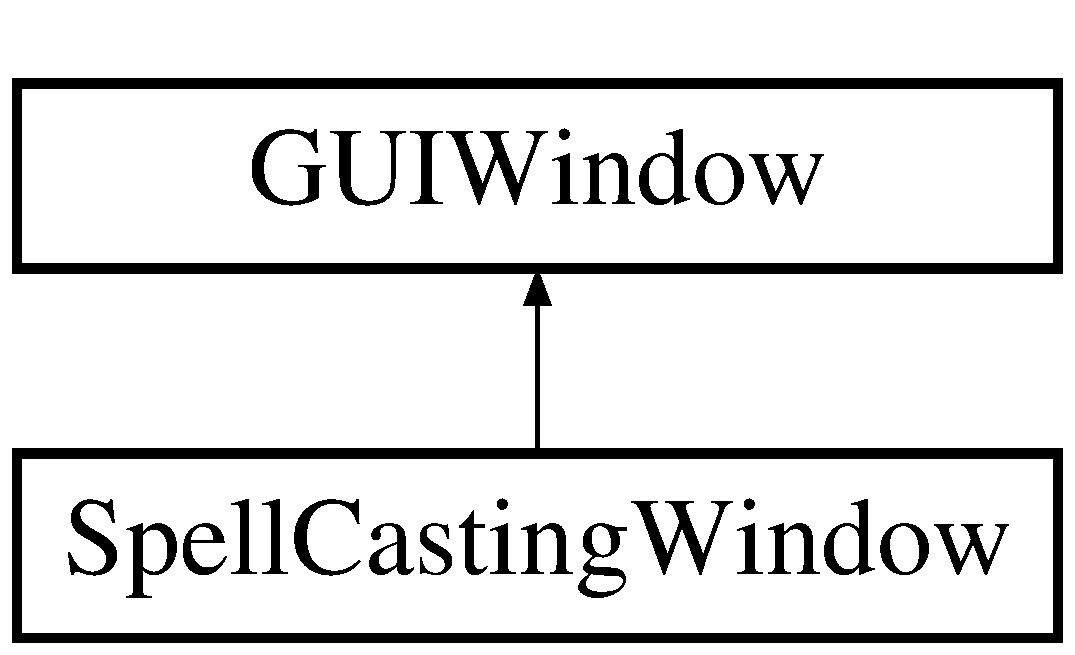
\includegraphics[height=2.000000cm]{class_spell_casting_window}
\end{center}
\end{figure}
\subsection*{Public Member Functions}
\begin{DoxyCompactItemize}
\item 
\hyperlink{class_spell_casting_window_aedd56bc34ff05cfdb6e068f17e23af6d}{Spell\+Casting\+Window} ()
\begin{DoxyCompactList}\small\item\em Constructor. \end{DoxyCompactList}\item 
\hyperlink{class_spell_casting_window_ad51f4c404269beb9959d66c5d5533791}{$\sim$\+Spell\+Casting\+Window} ()=default
\begin{DoxyCompactList}\small\item\em Destructor. \end{DoxyCompactList}\item 
void \hyperlink{class_spell_casting_window_a4c5bec658b7a9eb5f09e7de65c5841b5}{register\+\_\+spell} (const std\+::string \&)
\begin{DoxyCompactList}\small\item\em Appends a table name to the vector of all spell tables. \end{DoxyCompactList}\item 
void \hyperlink{class_spell_casting_window_a4168b2d0122273ba7f46a01dd5f37771}{set\+\_\+caster} (\hyperlink{class_spellcaster}{Spellcaster} $\ast$)
\begin{DoxyCompactList}\small\item\em Sets the caster instance used to cast the spells. \end{DoxyCompactList}\item 
void \hyperlink{class_spell_casting_window_a69be5be89e7db88045e4f2101e99c723}{deactivate\+\_\+current\+\_\+spell} ()
\begin{DoxyCompactList}\small\item\em Hides the \char`\"{}active\char`\"{} label. \end{DoxyCompactList}\item 
const std\+::vector$<$ std\+::string $>$ \& \hyperlink{class_spell_casting_window_a7c04e7d5264ad57bf457a7af90fe2751}{get\+\_\+spells} () const 
\begin{DoxyCompactList}\small\item\em Returns a vector containing the names of all unlocked spells. \end{DoxyCompactList}\item 
void \hyperlink{class_spell_casting_window_a7e7bd79dbe26ff5d34d6cb6715cdd3da}{clear\+\_\+spells} ()
\begin{DoxyCompactList}\small\item\em Removes all unlocked spell. \end{DoxyCompactList}\item 
bool \hyperlink{class_spell_casting_window_a53b66d15a7bfc705e895f004bd20d190}{dec\+\_\+selection} ()
\begin{DoxyCompactList}\small\item\em Decrements selection\+\_\+number\+\_\+ by one and updates the window. \end{DoxyCompactList}\item 
bool \hyperlink{class_spell_casting_window_a0f36135dc7e1dce4e404bbbe3b4097e1}{inc\+\_\+selection} ()
\begin{DoxyCompactList}\small\item\em Increments selection\+\_\+number\+\_\+ by one and updates the window. \end{DoxyCompactList}\item 
void \hyperlink{class_spell_casting_window_add2b56aea794690948c162f4ad060fc7}{set\+\_\+spell\+\_\+active} (int)
\begin{DoxyCompactList}\small\item\em Marks a given spell as active. \end{DoxyCompactList}\item 
void \hyperlink{class_spell_casting_window_ae4bb2064f95fbcac079f53e22e2de709}{cast} (int)
\begin{DoxyCompactList}\small\item\em Casts a spell at a given position in the roster. \end{DoxyCompactList}\end{DoxyCompactItemize}
\subsection*{Protected Member Functions}
\begin{DoxyCompactItemize}
\item 
void \hyperlink{class_spell_casting_window_a49a11d637aeef3e71036c3af9e459088}{init\+\_\+} () override
\begin{DoxyCompactList}\small\item\em Initializes the window and subscribes events. \end{DoxyCompactList}\end{DoxyCompactItemize}
\subsection*{Private Member Functions}
\begin{DoxyCompactItemize}
\item 
const std\+::string \& \hyperlink{class_spell_casting_window_a05004ce13e4b2417f2b6bab5098488be}{get\+\_\+spell\+\_\+} (std\+::size\+\_\+t)
\begin{DoxyCompactList}\small\item\em Range checked buildings\+\_\+ index access, returns the name of the building at a given index or \char`\"{}\+U\+N\+K\+N\+O\+W\+N\char`\"{} if the index is out of bounds. \end{DoxyCompactList}\item 
void \hyperlink{class_spell_casting_window_a2b90c5e701c4c00a3575935843d7c1c8}{update\+\_\+selection\+\_\+} ()
\begin{DoxyCompactList}\small\item\em Updates building names on the buttons. \end{DoxyCompactList}\end{DoxyCompactItemize}
\subsection*{Private Attributes}
\begin{DoxyCompactItemize}
\item 
std\+::vector$<$ std\+::string $>$ \hyperlink{class_spell_casting_window_ae155ce0f3e4dd38c6eeadede5d841d62}{spells\+\_\+}
\begin{DoxyCompactList}\small\item\em Names of all registered buildings. \end{DoxyCompactList}\item 
std\+::size\+\_\+t \hyperlink{class_spell_casting_window_a4ddb71ef5c7ca69e952bf49fbb0d41a7}{selection\+\_\+number\+\_\+}
\begin{DoxyCompactList}\small\item\em Number of the current rightmost selection. \end{DoxyCompactList}\item 
\hyperlink{classlpp_1_1_script}{lpp\+::\+Script} $\ast$ \hyperlink{class_spell_casting_window_ab31a088d48bc14324959e242ea2ff2d2}{script\+\_\+}
\begin{DoxyCompactList}\small\item\em Pointer to the scripting engine used for easier access. \end{DoxyCompactList}\item 
\hyperlink{class_spellcaster}{Spellcaster} $\ast$ \hyperlink{class_spell_casting_window_a4115e976e15588fce9cb953df23e69e5}{caster\+\_\+}
\begin{DoxyCompactList}\small\item\em Does the actual spell casting once a spell is selected in this window. \end{DoxyCompactList}\item 
int \hyperlink{class_spell_casting_window_adf1f5455827f746f5adbfb06cefc6c66}{curr\+\_\+active\+\_\+spell\+\_\+}
\begin{DoxyCompactList}\small\item\em Keeps track of the spell that is being currently casted. \end{DoxyCompactList}\end{DoxyCompactItemize}
\subsection*{Additional Inherited Members}


\subsection{Detailed Description}
Class representing the spell selection window, allows the player to cast registered (unlocked) spells. 

Definition at line 16 of file Spell\+Casting\+Window.\+hpp.



\subsection{Constructor \& Destructor Documentation}
\index{Spell\+Casting\+Window@{Spell\+Casting\+Window}!Spell\+Casting\+Window@{Spell\+Casting\+Window}}
\index{Spell\+Casting\+Window@{Spell\+Casting\+Window}!Spell\+Casting\+Window@{Spell\+Casting\+Window}}
\subsubsection[{\texorpdfstring{Spell\+Casting\+Window()}{SpellCastingWindow()}}]{\setlength{\rightskip}{0pt plus 5cm}Spell\+Casting\+Window\+::\+Spell\+Casting\+Window (
\begin{DoxyParamCaption}
{}
\end{DoxyParamCaption}
)}\hypertarget{class_spell_casting_window_aedd56bc34ff05cfdb6e068f17e23af6d}{}\label{class_spell_casting_window_aedd56bc34ff05cfdb6e068f17e23af6d}


Constructor. 



Definition at line 7 of file Spell\+Casting\+Window.\+cpp.

\index{Spell\+Casting\+Window@{Spell\+Casting\+Window}!````~Spell\+Casting\+Window@{$\sim$\+Spell\+Casting\+Window}}
\index{````~Spell\+Casting\+Window@{$\sim$\+Spell\+Casting\+Window}!Spell\+Casting\+Window@{Spell\+Casting\+Window}}
\subsubsection[{\texorpdfstring{$\sim$\+Spell\+Casting\+Window()=default}{~SpellCastingWindow()=default}}]{\setlength{\rightskip}{0pt plus 5cm}Spell\+Casting\+Window\+::$\sim$\+Spell\+Casting\+Window (
\begin{DoxyParamCaption}
{}
\end{DoxyParamCaption}
)\hspace{0.3cm}{\ttfamily [default]}}\hypertarget{class_spell_casting_window_ad51f4c404269beb9959d66c5d5533791}{}\label{class_spell_casting_window_ad51f4c404269beb9959d66c5d5533791}


Destructor. 



\subsection{Member Function Documentation}
\index{Spell\+Casting\+Window@{Spell\+Casting\+Window}!cast@{cast}}
\index{cast@{cast}!Spell\+Casting\+Window@{Spell\+Casting\+Window}}
\subsubsection[{\texorpdfstring{cast(int)}{cast(int)}}]{\setlength{\rightskip}{0pt plus 5cm}void Spell\+Casting\+Window\+::cast (
\begin{DoxyParamCaption}
\item[{int}]{spell\+\_\+num}
\end{DoxyParamCaption}
)}\hypertarget{class_spell_casting_window_ae4bb2064f95fbcac079f53e22e2de709}{}\label{class_spell_casting_window_ae4bb2064f95fbcac079f53e22e2de709}


Casts a spell at a given position in the roster. 


\begin{DoxyParams}{Parameters}
{\em The} & position of the spell (1-\/4). \\
\hline
\end{DoxyParams}


Definition at line 49 of file Spell\+Casting\+Window.\+cpp.

\index{Spell\+Casting\+Window@{Spell\+Casting\+Window}!clear\+\_\+spells@{clear\+\_\+spells}}
\index{clear\+\_\+spells@{clear\+\_\+spells}!Spell\+Casting\+Window@{Spell\+Casting\+Window}}
\subsubsection[{\texorpdfstring{clear\+\_\+spells()}{clear_spells()}}]{\setlength{\rightskip}{0pt plus 5cm}void Spell\+Casting\+Window\+::clear\+\_\+spells (
\begin{DoxyParamCaption}
{}
\end{DoxyParamCaption}
)}\hypertarget{class_spell_casting_window_a7e7bd79dbe26ff5d34d6cb6715cdd3da}{}\label{class_spell_casting_window_a7e7bd79dbe26ff5d34d6cb6715cdd3da}


Removes all unlocked spell. 



Definition at line 38 of file Spell\+Casting\+Window.\+cpp.

\index{Spell\+Casting\+Window@{Spell\+Casting\+Window}!deactivate\+\_\+current\+\_\+spell@{deactivate\+\_\+current\+\_\+spell}}
\index{deactivate\+\_\+current\+\_\+spell@{deactivate\+\_\+current\+\_\+spell}!Spell\+Casting\+Window@{Spell\+Casting\+Window}}
\subsubsection[{\texorpdfstring{deactivate\+\_\+current\+\_\+spell()}{deactivate_current_spell()}}]{\setlength{\rightskip}{0pt plus 5cm}void Spell\+Casting\+Window\+::deactivate\+\_\+current\+\_\+spell (
\begin{DoxyParamCaption}
{}
\end{DoxyParamCaption}
)}\hypertarget{class_spell_casting_window_a69be5be89e7db88045e4f2101e99c723}{}\label{class_spell_casting_window_a69be5be89e7db88045e4f2101e99c723}


Hides the \char`\"{}active\char`\"{} label. 



Definition at line 27 of file Spell\+Casting\+Window.\+cpp.

\index{Spell\+Casting\+Window@{Spell\+Casting\+Window}!dec\+\_\+selection@{dec\+\_\+selection}}
\index{dec\+\_\+selection@{dec\+\_\+selection}!Spell\+Casting\+Window@{Spell\+Casting\+Window}}
\subsubsection[{\texorpdfstring{dec\+\_\+selection()}{dec_selection()}}]{\setlength{\rightskip}{0pt plus 5cm}bool Spell\+Casting\+Window\+::dec\+\_\+selection (
\begin{DoxyParamCaption}
{}
\end{DoxyParamCaption}
)}\hypertarget{class_spell_casting_window_a53b66d15a7bfc705e895f004bd20d190}{}\label{class_spell_casting_window_a53b66d15a7bfc705e895f004bd20d190}


Decrements selection\+\_\+number\+\_\+ by one and updates the window. 



Definition at line 115 of file Spell\+Casting\+Window.\+cpp.

\index{Spell\+Casting\+Window@{Spell\+Casting\+Window}!get\+\_\+spell\+\_\+@{get\+\_\+spell\+\_\+}}
\index{get\+\_\+spell\+\_\+@{get\+\_\+spell\+\_\+}!Spell\+Casting\+Window@{Spell\+Casting\+Window}}
\subsubsection[{\texorpdfstring{get\+\_\+spell\+\_\+(std\+::size\+\_\+t)}{get_spell_(std::size_t)}}]{\setlength{\rightskip}{0pt plus 5cm}const std\+::string \& Spell\+Casting\+Window\+::get\+\_\+spell\+\_\+ (
\begin{DoxyParamCaption}
\item[{std\+::size\+\_\+t}]{index}
\end{DoxyParamCaption}
)\hspace{0.3cm}{\ttfamily [private]}}\hypertarget{class_spell_casting_window_a05004ce13e4b2417f2b6bab5098488be}{}\label{class_spell_casting_window_a05004ce13e4b2417f2b6bab5098488be}


Range checked buildings\+\_\+ index access, returns the name of the building at a given index or \char`\"{}\+U\+N\+K\+N\+O\+W\+N\char`\"{} if the index is out of bounds. 


\begin{DoxyParams}{Parameters}
{\em Index} & of the building in the buildings\+\_\+ vector. \\
\hline
\end{DoxyParams}


Definition at line 142 of file Spell\+Casting\+Window.\+cpp.

\index{Spell\+Casting\+Window@{Spell\+Casting\+Window}!get\+\_\+spells@{get\+\_\+spells}}
\index{get\+\_\+spells@{get\+\_\+spells}!Spell\+Casting\+Window@{Spell\+Casting\+Window}}
\subsubsection[{\texorpdfstring{get\+\_\+spells() const }{get_spells() const }}]{\setlength{\rightskip}{0pt plus 5cm}const std\+::vector$<$ std\+::string $>$ \& Spell\+Casting\+Window\+::get\+\_\+spells (
\begin{DoxyParamCaption}
{}
\end{DoxyParamCaption}
) const}\hypertarget{class_spell_casting_window_a7c04e7d5264ad57bf457a7af90fe2751}{}\label{class_spell_casting_window_a7c04e7d5264ad57bf457a7af90fe2751}


Returns a vector containing the names of all unlocked spells. 

(Used for serialization.) 

Definition at line 33 of file Spell\+Casting\+Window.\+cpp.

\index{Spell\+Casting\+Window@{Spell\+Casting\+Window}!inc\+\_\+selection@{inc\+\_\+selection}}
\index{inc\+\_\+selection@{inc\+\_\+selection}!Spell\+Casting\+Window@{Spell\+Casting\+Window}}
\subsubsection[{\texorpdfstring{inc\+\_\+selection()}{inc_selection()}}]{\setlength{\rightskip}{0pt plus 5cm}bool Spell\+Casting\+Window\+::inc\+\_\+selection (
\begin{DoxyParamCaption}
{}
\end{DoxyParamCaption}
)}\hypertarget{class_spell_casting_window_a0f36135dc7e1dce4e404bbbe3b4097e1}{}\label{class_spell_casting_window_a0f36135dc7e1dce4e404bbbe3b4097e1}


Increments selection\+\_\+number\+\_\+ by one and updates the window. 



Definition at line 129 of file Spell\+Casting\+Window.\+cpp.

\index{Spell\+Casting\+Window@{Spell\+Casting\+Window}!init\+\_\+@{init\+\_\+}}
\index{init\+\_\+@{init\+\_\+}!Spell\+Casting\+Window@{Spell\+Casting\+Window}}
\subsubsection[{\texorpdfstring{init\+\_\+() override}{init_() override}}]{\setlength{\rightskip}{0pt plus 5cm}void Spell\+Casting\+Window\+::init\+\_\+ (
\begin{DoxyParamCaption}
{}
\end{DoxyParamCaption}
)\hspace{0.3cm}{\ttfamily [override]}, {\ttfamily [protected]}, {\ttfamily [virtual]}}\hypertarget{class_spell_casting_window_a49a11d637aeef3e71036c3af9e459088}{}\label{class_spell_casting_window_a49a11d637aeef3e71036c3af9e459088}


Initializes the window and subscribes events. 



Implements \hyperlink{class_g_u_i_window_a2a7c011363f401a57a26cc7c7652bdfd}{G\+U\+I\+Window}.



Definition at line 61 of file Spell\+Casting\+Window.\+cpp.

\index{Spell\+Casting\+Window@{Spell\+Casting\+Window}!register\+\_\+spell@{register\+\_\+spell}}
\index{register\+\_\+spell@{register\+\_\+spell}!Spell\+Casting\+Window@{Spell\+Casting\+Window}}
\subsubsection[{\texorpdfstring{register\+\_\+spell(const std\+::string \&)}{register_spell(const std::string &)}}]{\setlength{\rightskip}{0pt plus 5cm}void Spell\+Casting\+Window\+::register\+\_\+spell (
\begin{DoxyParamCaption}
\item[{const std\+::string \&}]{name}
\end{DoxyParamCaption}
)}\hypertarget{class_spell_casting_window_a4c5bec658b7a9eb5f09e7de65c5841b5}{}\label{class_spell_casting_window_a4c5bec658b7a9eb5f09e7de65c5841b5}


Appends a table name to the vector of all spell tables. 


\begin{DoxyParams}{Parameters}
{\em Name} & of the table to register. \\
\hline
\end{DoxyParams}


Definition at line 11 of file Spell\+Casting\+Window.\+cpp.

\index{Spell\+Casting\+Window@{Spell\+Casting\+Window}!set\+\_\+caster@{set\+\_\+caster}}
\index{set\+\_\+caster@{set\+\_\+caster}!Spell\+Casting\+Window@{Spell\+Casting\+Window}}
\subsubsection[{\texorpdfstring{set\+\_\+caster(\+Spellcaster $\ast$)}{set_caster(Spellcaster *)}}]{\setlength{\rightskip}{0pt plus 5cm}void Spell\+Casting\+Window\+::set\+\_\+caster (
\begin{DoxyParamCaption}
\item[{{\bf Spellcaster} $\ast$}]{caster}
\end{DoxyParamCaption}
)}\hypertarget{class_spell_casting_window_a4168b2d0122273ba7f46a01dd5f37771}{}\label{class_spell_casting_window_a4168b2d0122273ba7f46a01dd5f37771}


Sets the caster instance used to cast the spells. 


\begin{DoxyParams}{Parameters}
{\em The} & new spell caster. \\
\hline
\end{DoxyParams}


Definition at line 22 of file Spell\+Casting\+Window.\+cpp.

\index{Spell\+Casting\+Window@{Spell\+Casting\+Window}!set\+\_\+spell\+\_\+active@{set\+\_\+spell\+\_\+active}}
\index{set\+\_\+spell\+\_\+active@{set\+\_\+spell\+\_\+active}!Spell\+Casting\+Window@{Spell\+Casting\+Window}}
\subsubsection[{\texorpdfstring{set\+\_\+spell\+\_\+active(int)}{set_spell_active(int)}}]{\setlength{\rightskip}{0pt plus 5cm}void Spell\+Casting\+Window\+::set\+\_\+spell\+\_\+active (
\begin{DoxyParamCaption}
\item[{int}]{val}
\end{DoxyParamCaption}
)}\hypertarget{class_spell_casting_window_add2b56aea794690948c162f4ad060fc7}{}\label{class_spell_casting_window_add2b56aea794690948c162f4ad060fc7}


Marks a given spell as active. 


\begin{DoxyParams}{Parameters}
{\em Position} & of the spell in the current view (0-\/3). \\
\hline
\end{DoxyParams}


Definition at line 182 of file Spell\+Casting\+Window.\+cpp.

\index{Spell\+Casting\+Window@{Spell\+Casting\+Window}!update\+\_\+selection\+\_\+@{update\+\_\+selection\+\_\+}}
\index{update\+\_\+selection\+\_\+@{update\+\_\+selection\+\_\+}!Spell\+Casting\+Window@{Spell\+Casting\+Window}}
\subsubsection[{\texorpdfstring{update\+\_\+selection\+\_\+()}{update_selection_()}}]{\setlength{\rightskip}{0pt plus 5cm}void Spell\+Casting\+Window\+::update\+\_\+selection\+\_\+ (
\begin{DoxyParamCaption}
{}
\end{DoxyParamCaption}
)\hspace{0.3cm}{\ttfamily [private]}}\hypertarget{class_spell_casting_window_a2b90c5e701c4c00a3575935843d7c1c8}{}\label{class_spell_casting_window_a2b90c5e701c4c00a3575935843d7c1c8}


Updates building names on the buttons. 



Definition at line 152 of file Spell\+Casting\+Window.\+cpp.



\subsection{Member Data Documentation}
\index{Spell\+Casting\+Window@{Spell\+Casting\+Window}!caster\+\_\+@{caster\+\_\+}}
\index{caster\+\_\+@{caster\+\_\+}!Spell\+Casting\+Window@{Spell\+Casting\+Window}}
\subsubsection[{\texorpdfstring{caster\+\_\+}{caster_}}]{\setlength{\rightskip}{0pt plus 5cm}{\bf Spellcaster}$\ast$ Spell\+Casting\+Window\+::caster\+\_\+\hspace{0.3cm}{\ttfamily [private]}}\hypertarget{class_spell_casting_window_a4115e976e15588fce9cb953df23e69e5}{}\label{class_spell_casting_window_a4115e976e15588fce9cb953df23e69e5}


Does the actual spell casting once a spell is selected in this window. 



Definition at line 124 of file Spell\+Casting\+Window.\+hpp.

\index{Spell\+Casting\+Window@{Spell\+Casting\+Window}!curr\+\_\+active\+\_\+spell\+\_\+@{curr\+\_\+active\+\_\+spell\+\_\+}}
\index{curr\+\_\+active\+\_\+spell\+\_\+@{curr\+\_\+active\+\_\+spell\+\_\+}!Spell\+Casting\+Window@{Spell\+Casting\+Window}}
\subsubsection[{\texorpdfstring{curr\+\_\+active\+\_\+spell\+\_\+}{curr_active_spell_}}]{\setlength{\rightskip}{0pt plus 5cm}int Spell\+Casting\+Window\+::curr\+\_\+active\+\_\+spell\+\_\+\hspace{0.3cm}{\ttfamily [private]}}\hypertarget{class_spell_casting_window_adf1f5455827f746f5adbfb06cefc6c66}{}\label{class_spell_casting_window_adf1f5455827f746f5adbfb06cefc6c66}


Keeps track of the spell that is being currently casted. 



Definition at line 129 of file Spell\+Casting\+Window.\+hpp.

\index{Spell\+Casting\+Window@{Spell\+Casting\+Window}!script\+\_\+@{script\+\_\+}}
\index{script\+\_\+@{script\+\_\+}!Spell\+Casting\+Window@{Spell\+Casting\+Window}}
\subsubsection[{\texorpdfstring{script\+\_\+}{script_}}]{\setlength{\rightskip}{0pt plus 5cm}{\bf lpp\+::\+Script}$\ast$ Spell\+Casting\+Window\+::script\+\_\+\hspace{0.3cm}{\ttfamily [private]}}\hypertarget{class_spell_casting_window_ab31a088d48bc14324959e242ea2ff2d2}{}\label{class_spell_casting_window_ab31a088d48bc14324959e242ea2ff2d2}


Pointer to the scripting engine used for easier access. 



Definition at line 118 of file Spell\+Casting\+Window.\+hpp.

\index{Spell\+Casting\+Window@{Spell\+Casting\+Window}!selection\+\_\+number\+\_\+@{selection\+\_\+number\+\_\+}}
\index{selection\+\_\+number\+\_\+@{selection\+\_\+number\+\_\+}!Spell\+Casting\+Window@{Spell\+Casting\+Window}}
\subsubsection[{\texorpdfstring{selection\+\_\+number\+\_\+}{selection_number_}}]{\setlength{\rightskip}{0pt plus 5cm}std\+::size\+\_\+t Spell\+Casting\+Window\+::selection\+\_\+number\+\_\+\hspace{0.3cm}{\ttfamily [private]}}\hypertarget{class_spell_casting_window_a4ddb71ef5c7ca69e952bf49fbb0d41a7}{}\label{class_spell_casting_window_a4ddb71ef5c7ca69e952bf49fbb0d41a7}


Number of the current rightmost selection. 

The window shows buildings with indices $<$selection\+\_\+number\+\_\+ -\/ 3, selection\+\_\+number\+\_\+$>$. 

Definition at line 112 of file Spell\+Casting\+Window.\+hpp.

\index{Spell\+Casting\+Window@{Spell\+Casting\+Window}!spells\+\_\+@{spells\+\_\+}}
\index{spells\+\_\+@{spells\+\_\+}!Spell\+Casting\+Window@{Spell\+Casting\+Window}}
\subsubsection[{\texorpdfstring{spells\+\_\+}{spells_}}]{\setlength{\rightskip}{0pt plus 5cm}std\+::vector$<$std\+::string$>$ Spell\+Casting\+Window\+::spells\+\_\+\hspace{0.3cm}{\ttfamily [private]}}\hypertarget{class_spell_casting_window_ae155ce0f3e4dd38c6eeadede5d841d62}{}\label{class_spell_casting_window_ae155ce0f3e4dd38c6eeadede5d841d62}


Names of all registered buildings. 



Definition at line 106 of file Spell\+Casting\+Window.\+hpp.



The documentation for this class was generated from the following files\+:\begin{DoxyCompactItemize}
\item 
gui/Spell\+Casting\+Window.\+hpp\item 
gui/Spell\+Casting\+Window.\+cpp\end{DoxyCompactItemize}

\hypertarget{struct_spell_component}{}\section{Spell\+Component Struct Reference}
\label{struct_spell_component}\index{Spell\+Component@{Spell\+Component}}


Allows an entity to periodically cast a spell.  




{\ttfamily \#include $<$Components.\+hpp$>$}

\subsection*{Public Member Functions}
\begin{DoxyCompactItemize}
\item 
{\bfseries Spell\+Component} (std\+::string \&\&b=\char`\"{}E\+R\+R\+OR\char`\"{}, tdt\+::real cd=0.f)\hypertarget{struct_spell_component_aa3116e6a22bee9171a7f8457b2aee7d6}{}\label{struct_spell_component_aa3116e6a22bee9171a7f8457b2aee7d6}

\item 
{\bfseries Spell\+Component} (const \hyperlink{struct_spell_component}{Spell\+Component} \&)=default\hypertarget{struct_spell_component_a94388b3be342e62032dadca4f7295d24}{}\label{struct_spell_component_a94388b3be342e62032dadca4f7295d24}

\item 
{\bfseries Spell\+Component} (\hyperlink{struct_spell_component}{Spell\+Component} \&\&)=default\hypertarget{struct_spell_component_a116938e539ae883ac408c2425a5535c8}{}\label{struct_spell_component_a116938e539ae883ac408c2425a5535c8}

\item 
\hyperlink{struct_spell_component}{Spell\+Component} \& {\bfseries operator=} (const \hyperlink{struct_spell_component}{Spell\+Component} \&)=default\hypertarget{struct_spell_component_a98b185f74b044ac0e6a42547c421506e}{}\label{struct_spell_component_a98b185f74b044ac0e6a42547c421506e}

\item 
\hyperlink{struct_spell_component}{Spell\+Component} \& {\bfseries operator=} (\hyperlink{struct_spell_component}{Spell\+Component} \&\&)=default\hypertarget{struct_spell_component_a6ddd65b933d79544d396c8dd0652de05}{}\label{struct_spell_component_a6ddd65b933d79544d396c8dd0652de05}

\end{DoxyCompactItemize}
\subsection*{Public Attributes}
\begin{DoxyCompactItemize}
\item 
std\+::string {\bfseries blueprint}\hypertarget{struct_spell_component_a7abaab12e30aeb0963b90a40e85d3e12}{}\label{struct_spell_component_a7abaab12e30aeb0963b90a40e85d3e12}

\item 
tdt\+::real {\bfseries cd\+\_\+time}\hypertarget{struct_spell_component_a408795d904893c26a19162827064edc2}{}\label{struct_spell_component_a408795d904893c26a19162827064edc2}

\item 
tdt\+::real {\bfseries cooldown}\hypertarget{struct_spell_component_a1d83c588bb504f78cf9f2ec9999651be}{}\label{struct_spell_component_a1d83c588bb504f78cf9f2ec9999651be}

\end{DoxyCompactItemize}
\subsection*{Static Public Attributes}
\begin{DoxyCompactItemize}
\item 
static constexpr int {\bfseries type} = 10\hypertarget{struct_spell_component_aeba2074e07a2694120db7e715b8129f9}{}\label{struct_spell_component_aeba2074e07a2694120db7e715b8129f9}

\end{DoxyCompactItemize}


\subsection{Detailed Description}
Allows an entity to periodically cast a spell. 

Definition at line 272 of file Components.\+hpp.



The documentation for this struct was generated from the following file\+:\begin{DoxyCompactItemize}
\item 
Components.\+hpp\end{DoxyCompactItemize}

\hypertarget{struct_structure_component}{}\section{Structure\+Component Struct Reference}
\label{struct_structure_component}\index{Structure\+Component@{Structure\+Component}}


Defines a building (or a wall), by holding it\textquotesingle{}s radius (of the area it takes in the grid) and vector of nodes that it sits on.  




{\ttfamily \#include $<$Components.\+hpp$>$}

\subsection*{Public Member Functions}
\begin{DoxyCompactItemize}
\item 
{\bfseries Structure\+Component} (tdt\+::uint r=1, bool wt=false)\hypertarget{struct_structure_component_a4bcfdb3d4a8b2ffdc9aeac79fa18f441}{}\label{struct_structure_component_a4bcfdb3d4a8b2ffdc9aeac79fa18f441}

\item 
{\bfseries Structure\+Component} (const \hyperlink{struct_structure_component}{Structure\+Component} \&)=default\hypertarget{struct_structure_component_a6d71fc7a071b14088aaf870bc5f5e2b0}{}\label{struct_structure_component_a6d71fc7a071b14088aaf870bc5f5e2b0}

\item 
{\bfseries Structure\+Component} (\hyperlink{struct_structure_component}{Structure\+Component} \&\&)=default\hypertarget{struct_structure_component_a0fdcf5b99834b3d6464f78c23aef4a21}{}\label{struct_structure_component_a0fdcf5b99834b3d6464f78c23aef4a21}

\item 
\hyperlink{struct_structure_component}{Structure\+Component} \& {\bfseries operator=} (const \hyperlink{struct_structure_component}{Structure\+Component} \&)=default\hypertarget{struct_structure_component_ad62a4efd8d3237d0e1c565660072a515}{}\label{struct_structure_component_ad62a4efd8d3237d0e1c565660072a515}

\item 
\hyperlink{struct_structure_component}{Structure\+Component} \& {\bfseries operator=} (\hyperlink{struct_structure_component}{Structure\+Component} \&\&)=default\hypertarget{struct_structure_component_a2e4612b5c07afcdcbde0b183a1e5cc85}{}\label{struct_structure_component_a2e4612b5c07afcdcbde0b183a1e5cc85}

\end{DoxyCompactItemize}
\subsection*{Public Attributes}
\begin{DoxyCompactItemize}
\item 
tdt\+::uint {\bfseries radius}\hypertarget{struct_structure_component_a1ca0ec718c0c0c94e132194d54ff39c1}{}\label{struct_structure_component_a1ca0ec718c0c0c94e132194d54ff39c1}

\item 
bool {\bfseries walk\+\_\+through}\hypertarget{struct_structure_component_ad366ea0fb8acab2ca163bf427680ddd2}{}\label{struct_structure_component_ad366ea0fb8acab2ca163bf427680ddd2}

\item 
std\+::vector$<$ tdt\+::uint $>$ {\bfseries residences}\hypertarget{struct_structure_component_a476d7a4d964a344a0195563e252602c1}{}\label{struct_structure_component_a476d7a4d964a344a0195563e252602c1}

\end{DoxyCompactItemize}
\subsection*{Static Public Attributes}
\begin{DoxyCompactItemize}
\item 
static constexpr int {\bfseries type} = 17\hypertarget{struct_structure_component_afd9702d5889f23c1fb020e41cff8c3f7}{}\label{struct_structure_component_afd9702d5889f23c1fb020e41cff8c3f7}

\end{DoxyCompactItemize}


\subsection{Detailed Description}
Defines a building (or a wall), by holding it\textquotesingle{}s radius (of the area it takes in the grid) and vector of nodes that it sits on. 

Definition at line 440 of file Components.\+hpp.



The documentation for this struct was generated from the following file\+:\begin{DoxyCompactItemize}
\item 
Components.\+hpp\end{DoxyCompactItemize}

\hypertarget{class_system}{}\section{System Class Reference}
\label{class_system}\index{System@{System}}


Parent class of all systems.  




{\ttfamily \#include $<$System.\+hpp$>$}

Inheritance diagram for System\+:\begin{figure}[H]
\begin{center}
\leavevmode
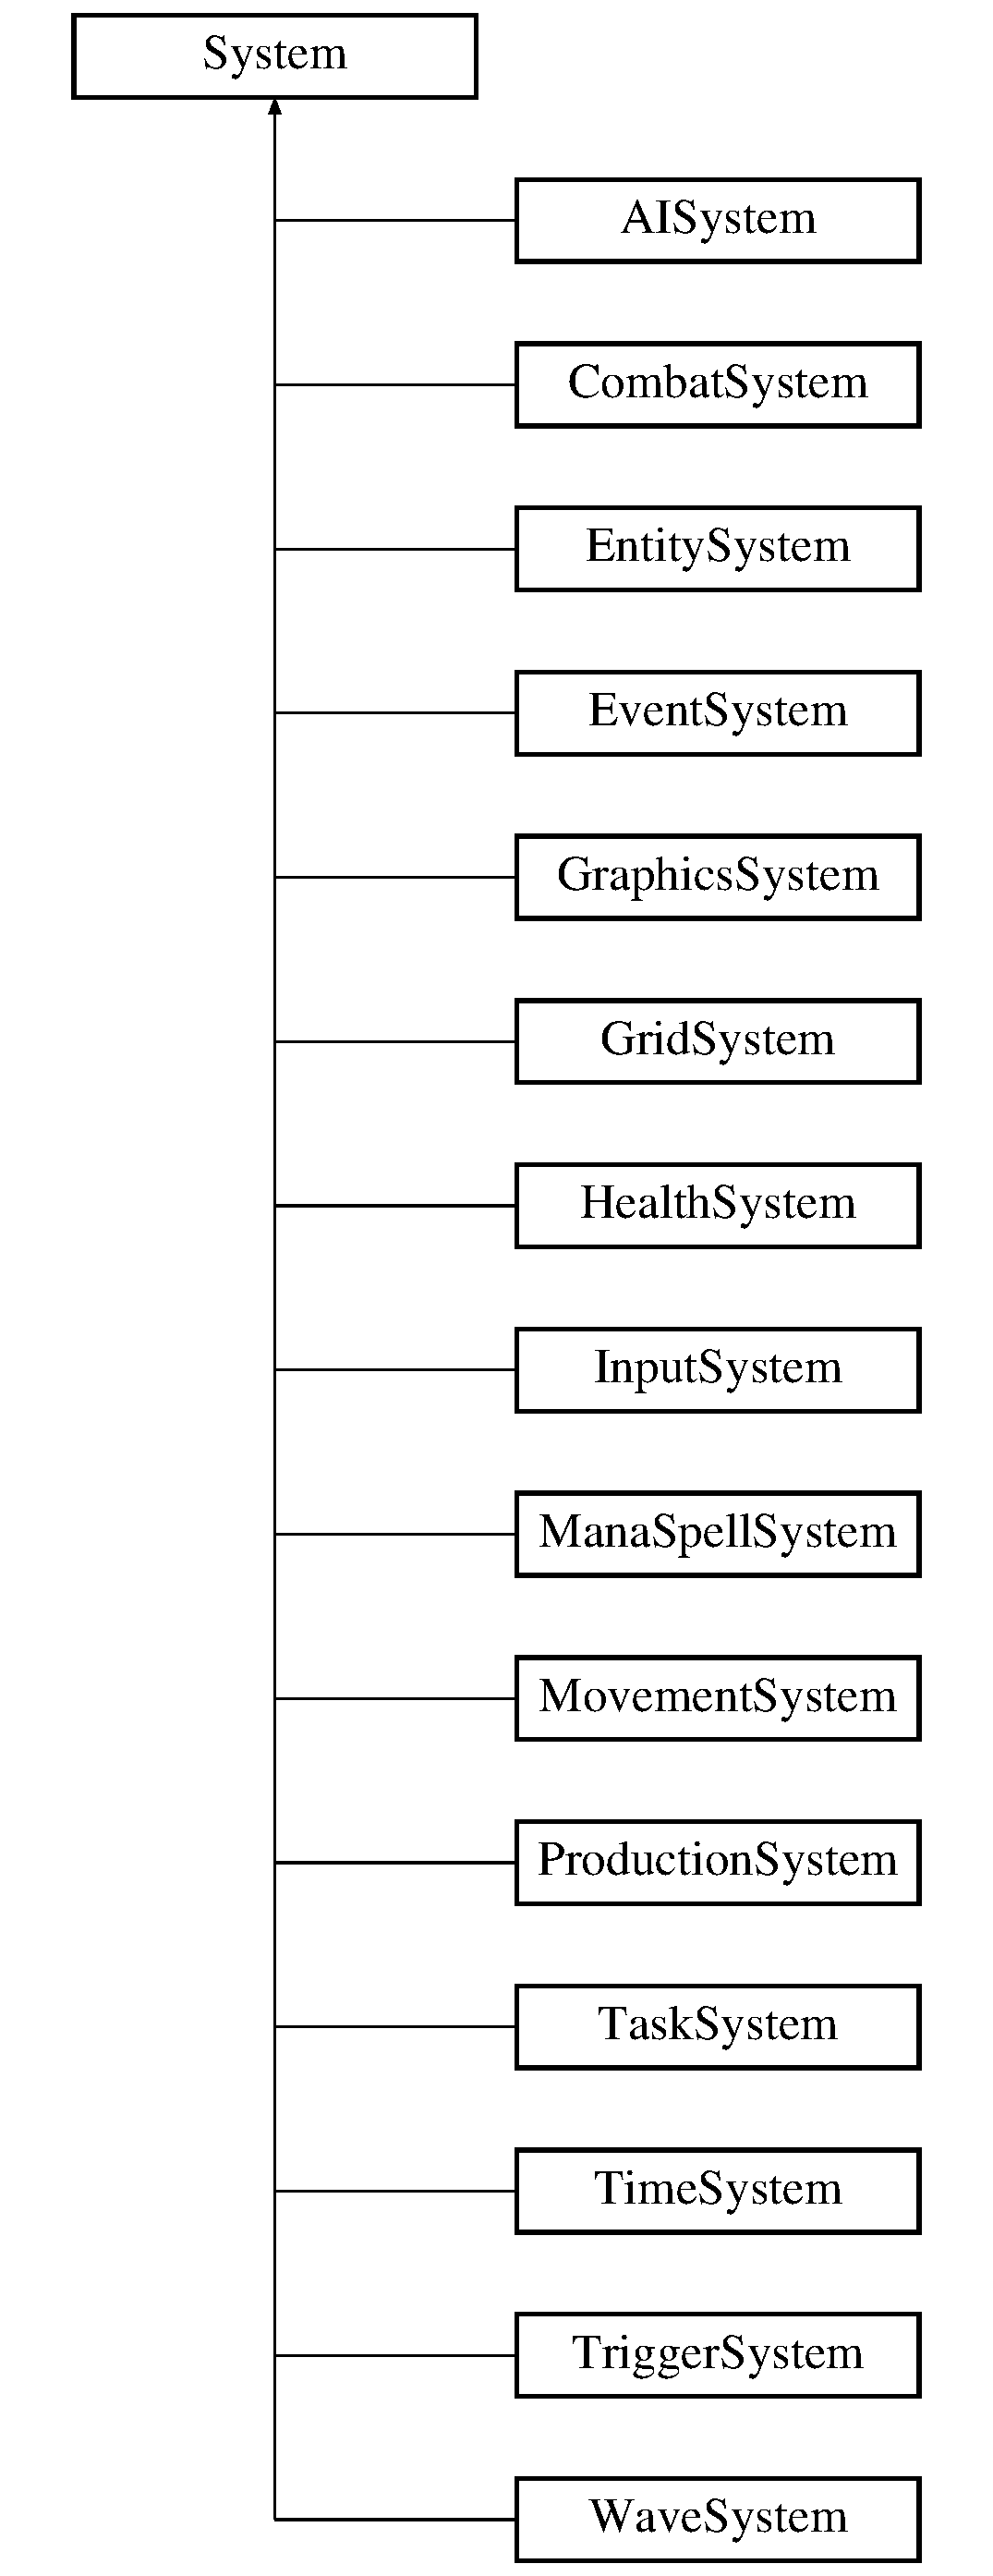
\includegraphics[height=12.000000cm]{class_system}
\end{center}
\end{figure}
\subsection*{Public Member Functions}
\begin{DoxyCompactItemize}
\item 
virtual void \hyperlink{class_system_a6d54c9bd38eb43d620a1451cb0925472}{update} (tdt\+::real)=0
\begin{DoxyCompactList}\small\item\em Updates the system. \end{DoxyCompactList}\item 
virtual \hyperlink{class_system_ad652aa3c77ed19131f598a7355c0939a}{$\sim$\+System} ()=default
\begin{DoxyCompactList}\small\item\em Destructor. \end{DoxyCompactList}\end{DoxyCompactItemize}


\subsection{Detailed Description}
Parent class of all systems. 

Definition at line 8 of file System.\+hpp.



\subsection{Constructor \& Destructor Documentation}
\index{System@{System}!````~System@{$\sim$\+System}}
\index{````~System@{$\sim$\+System}!System@{System}}
\subsubsection[{\texorpdfstring{$\sim$\+System()=default}{~System()=default}}]{\setlength{\rightskip}{0pt plus 5cm}virtual System\+::$\sim$\+System (
\begin{DoxyParamCaption}
{}
\end{DoxyParamCaption}
)\hspace{0.3cm}{\ttfamily [virtual]}, {\ttfamily [default]}}\hypertarget{class_system_ad652aa3c77ed19131f598a7355c0939a}{}\label{class_system_ad652aa3c77ed19131f598a7355c0939a}


Destructor. 



\subsection{Member Function Documentation}
\index{System@{System}!update@{update}}
\index{update@{update}!System@{System}}
\subsubsection[{\texorpdfstring{update(tdt\+::real)=0}{update(tdt::real)=0}}]{\setlength{\rightskip}{0pt plus 5cm}virtual void System\+::update (
\begin{DoxyParamCaption}
\item[{tdt\+::real}]{}
\end{DoxyParamCaption}
)\hspace{0.3cm}{\ttfamily [pure virtual]}}\hypertarget{class_system_a6d54c9bd38eb43d620a1451cb0925472}{}\label{class_system_a6d54c9bd38eb43d620a1451cb0925472}


Updates the system. 


\begin{DoxyParams}{Parameters}
{\em Time} & since the last frame. \\
\hline
\end{DoxyParams}


Implemented in \hyperlink{class_combat_system_a2c284a065f150a9fb67dae0f1229db37}{Combat\+System}, \hyperlink{class_entity_system_aa51808181d7c66baea07cec41c17b4cd}{Entity\+System}, \hyperlink{class_wave_system_a98df4388628f2618db5c2aa18ce67c11}{Wave\+System}, \hyperlink{class_input_system_a6ee8dd556fa9352321197412b186c0c1}{Input\+System}, \hyperlink{class_task_system_a7dda98e47b288ace9709f0d47a1a66c2}{Task\+System}, \hyperlink{class_production_system_ad8d47ea05eeb8504a58c2f68f9285c35}{Production\+System}, \hyperlink{class_grid_system_a4a63a4d431ce96dadcbb1603a88bf71b}{Grid\+System}, \hyperlink{class_trigger_system_ac85976839b1316705e1a493fb40c3ef2}{Trigger\+System}, \hyperlink{class_health_system_a20f7adc2c2ab6e92ba8dd02e3ec95ba2}{Health\+System}, \hyperlink{class_mana_spell_system_a72ff0244c7ed729843fc82dde04b3477}{Mana\+Spell\+System}, \hyperlink{class_a_i_system_a2c979ff5f110c79326f17f95c4b655d9}{A\+I\+System}, \hyperlink{class_graphics_system_a1b5bf7d5928bcc00d90dec8be3866440}{Graphics\+System}, \hyperlink{class_movement_system_a005915a7fff5eaf8f1e644e07ccda9e4}{Movement\+System}, \hyperlink{class_time_system_a628f5adf452ee0a1636ef60d78821293}{Time\+System}, and \hyperlink{class_event_system_a1410963080a61fdbafc406100dc17d8d}{Event\+System}.



The documentation for this class was generated from the following file\+:\begin{DoxyCompactItemize}
\item 
systems/System.\+hpp\end{DoxyCompactItemize}

\hypertarget{struct_task_component}{}\section{Task\+Component Struct Reference}
\label{struct_task_component}\index{Task\+Component@{Task\+Component}}


Defines a task by giving it a type, source (the task handler) and a target (subject of the task).  




{\ttfamily \#include $<$Components.\+hpp$>$}

\subsection*{Public Member Functions}
\begin{DoxyCompactItemize}
\item 
{\bfseries Task\+Component} (tdt\+::uint target\+\_\+id=Component\+::\+N\+O\+\_\+\+E\+N\+T\+I\+TY, tdt\+::uint source\+\_\+id=Component\+::\+N\+O\+\_\+\+E\+N\+T\+I\+TY, T\+A\+S\+K\+\_\+\+T\+Y\+PE t\+\_\+type=T\+A\+S\+K\+\_\+\+T\+Y\+P\+E\+::\+N\+O\+NE)\hypertarget{struct_task_component_aa1dc17778221f9c171d027d4ca669e18}{}\label{struct_task_component_aa1dc17778221f9c171d027d4ca669e18}

\item 
{\bfseries Task\+Component} (const \hyperlink{struct_task_component}{Task\+Component} \&)=default\hypertarget{struct_task_component_a5bea8c0a5cf8c094f8a16d261b9ddbf2}{}\label{struct_task_component_a5bea8c0a5cf8c094f8a16d261b9ddbf2}

\item 
{\bfseries Task\+Component} (\hyperlink{struct_task_component}{Task\+Component} \&\&)=default\hypertarget{struct_task_component_aa94f3b8b0ca8cdddb40fdea361afa572}{}\label{struct_task_component_aa94f3b8b0ca8cdddb40fdea361afa572}

\item 
\hyperlink{struct_task_component}{Task\+Component} \& {\bfseries operator=} (const \hyperlink{struct_task_component}{Task\+Component} \&)=default\hypertarget{struct_task_component_ad85f3e8dd2d5f057e375b79acf55cb2f}{}\label{struct_task_component_ad85f3e8dd2d5f057e375b79acf55cb2f}

\item 
\hyperlink{struct_task_component}{Task\+Component} \& {\bfseries operator=} (\hyperlink{struct_task_component}{Task\+Component} \&\&)=default\hypertarget{struct_task_component_a9fe9676d27cf6b8f7f30b44eaf194bf2}{}\label{struct_task_component_a9fe9676d27cf6b8f7f30b44eaf194bf2}

\end{DoxyCompactItemize}
\subsection*{Public Attributes}
\begin{DoxyCompactItemize}
\item 
T\+A\+S\+K\+\_\+\+T\+Y\+PE {\bfseries task\+\_\+type}\hypertarget{struct_task_component_a8cac16b519aaa5976c3067ad8c82dd4a}{}\label{struct_task_component_a8cac16b519aaa5976c3067ad8c82dd4a}

\item 
tdt\+::uint {\bfseries source}\hypertarget{struct_task_component_a37a5e40f9725acdb7c1ec02a1dc2e4db}{}\label{struct_task_component_a37a5e40f9725acdb7c1ec02a1dc2e4db}

\item 
tdt\+::uint {\bfseries target}\hypertarget{struct_task_component_a4d10619d204daefabb89d566cb3b99fc}{}\label{struct_task_component_a4d10619d204daefabb89d566cb3b99fc}

\item 
bool {\bfseries complete}\hypertarget{struct_task_component_a0ebf4b1137c1ef072369289f1c8580fe}{}\label{struct_task_component_a0ebf4b1137c1ef072369289f1c8580fe}

\end{DoxyCompactItemize}
\subsection*{Static Public Attributes}
\begin{DoxyCompactItemize}
\item 
static constexpr int {\bfseries type} = 15\hypertarget{struct_task_component_a931d8eea55f368a3eadbeb988dcaa7ec}{}\label{struct_task_component_a931d8eea55f368a3eadbeb988dcaa7ec}

\end{DoxyCompactItemize}


\subsection{Detailed Description}
Defines a task by giving it a type, source (the task handler) and a target (subject of the task). 

Handling of these tasks is done via the \hyperlink{struct_task_handler_component}{Task\+Handler\+Component} below. 

Definition at line 390 of file Components.\+hpp.



The documentation for this struct was generated from the following file\+:\begin{DoxyCompactItemize}
\item 
Components.\+hpp\end{DoxyCompactItemize}

\hypertarget{struct_task_handler_component}{}\section{Task\+Handler\+Component Struct Reference}
\label{struct_task_handler_component}\index{Task\+Handler\+Component@{Task\+Handler\+Component}}


Task queue and register of possible tasks, every entity that is able to actually do something on it\textquotesingle{}s own should have it.  




{\ttfamily \#include $<$Components.\+hpp$>$}

\subsection*{Public Member Functions}
\begin{DoxyCompactItemize}
\item 
{\bfseries Task\+Handler\+Component} (std\+::string \&\&b=\char`\"{}E\+R\+R\+OR\char`\"{})\hypertarget{struct_task_handler_component_a6e2e537bd2a20dd39e82671725531647}{}\label{struct_task_handler_component_a6e2e537bd2a20dd39e82671725531647}

\item 
{\bfseries Task\+Handler\+Component} (const \hyperlink{struct_task_handler_component}{Task\+Handler\+Component} \&)=default\hypertarget{struct_task_handler_component_a90f2e87a272be1ad40912cb628c917aa}{}\label{struct_task_handler_component_a90f2e87a272be1ad40912cb628c917aa}

\item 
{\bfseries Task\+Handler\+Component} (\hyperlink{struct_task_handler_component}{Task\+Handler\+Component} \&\&)=default\hypertarget{struct_task_handler_component_a8578d55c4499bf925c7e5d35d7c774d4}{}\label{struct_task_handler_component_a8578d55c4499bf925c7e5d35d7c774d4}

\item 
\hyperlink{struct_task_handler_component}{Task\+Handler\+Component} \& {\bfseries operator=} (const \hyperlink{struct_task_handler_component}{Task\+Handler\+Component} \&)=default\hypertarget{struct_task_handler_component_aa4187b1d9fbba8bddae9be31be6c234a}{}\label{struct_task_handler_component_aa4187b1d9fbba8bddae9be31be6c234a}

\item 
\hyperlink{struct_task_handler_component}{Task\+Handler\+Component} \& {\bfseries operator=} (\hyperlink{struct_task_handler_component}{Task\+Handler\+Component} \&\&)=default\hypertarget{struct_task_handler_component_acdc159bc139d71cf2ce26c247520234f}{}\label{struct_task_handler_component_acdc159bc139d71cf2ce26c247520234f}

\end{DoxyCompactItemize}
\subsection*{Public Attributes}
\begin{DoxyCompactItemize}
\item 
tdt\+::uint {\bfseries curr\+\_\+task}\hypertarget{struct_task_handler_component_a63aefaaa68be4e2f46fa142acb1bd4f8}{}\label{struct_task_handler_component_a63aefaaa68be4e2f46fa142acb1bd4f8}

\item 
std\+::bitset$<$(int) T\+A\+S\+K\+\_\+\+T\+Y\+P\+E\+::\+C\+O\+U\+NT $>$ {\bfseries possible\+\_\+tasks}\hypertarget{struct_task_handler_component_ae4ece22f8aa6b800915ce49743c5bb21}{}\label{struct_task_handler_component_ae4ece22f8aa6b800915ce49743c5bb21}

\item 
std\+::deque$<$ tdt\+::uint $>$ {\bfseries task\+\_\+queue}\hypertarget{struct_task_handler_component_a9754b7c65f6992afa1e5ade63d28f626}{}\label{struct_task_handler_component_a9754b7c65f6992afa1e5ade63d28f626}

\item 
bool {\bfseries busy}\hypertarget{struct_task_handler_component_a6481b2a8188abc40d618a50cb37e7164}{}\label{struct_task_handler_component_a6481b2a8188abc40d618a50cb37e7164}

\item 
std\+::string {\bfseries blueprint}\hypertarget{struct_task_handler_component_a0530d5bca650606f819e614fe2dab3a8}{}\label{struct_task_handler_component_a0530d5bca650606f819e614fe2dab3a8}

\end{DoxyCompactItemize}
\subsection*{Static Public Attributes}
\begin{DoxyCompactItemize}
\item 
static constexpr int {\bfseries type} = 16\hypertarget{struct_task_handler_component_a12e6522dc9c13999683e1f624fc27dd0}{}\label{struct_task_handler_component_a12e6522dc9c13999683e1f624fc27dd0}

\end{DoxyCompactItemize}


\subsection{Detailed Description}
Task queue and register of possible tasks, every entity that is able to actually do something on it\textquotesingle{}s own should have it. 

Definition at line 415 of file Components.\+hpp.



The documentation for this struct was generated from the following file\+:\begin{DoxyCompactItemize}
\item 
Components.\+hpp\end{DoxyCompactItemize}

\hypertarget{class_task_system}{}\section{Task\+System Class Reference}
\label{class_task_system}\index{Task\+System@{Task\+System}}


\hyperlink{class_system}{System} managing all entities with the \hyperlink{struct_task_component}{Task\+Component}, their creation, assignment, lifetime checks and canceling.  




{\ttfamily \#include $<$Task\+System.\+hpp$>$}

Inheritance diagram for Task\+System\+:\begin{figure}[H]
\begin{center}
\leavevmode
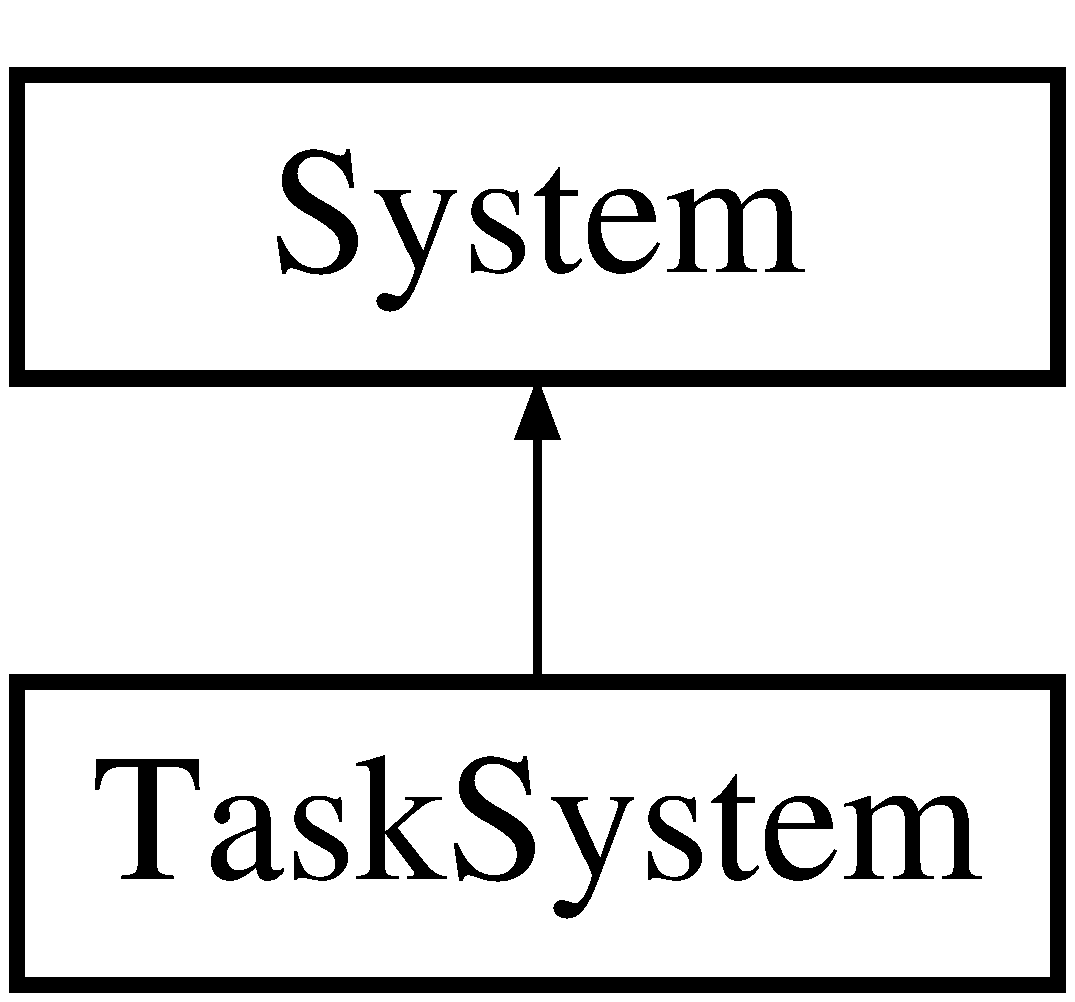
\includegraphics[height=2.000000cm]{class_task_system}
\end{center}
\end{figure}
\subsection*{Public Member Functions}
\begin{DoxyCompactItemize}
\item 
\hyperlink{class_task_system_a07a8d2cbffd5c271f26f4ba5f5398db3}{Task\+System} (\hyperlink{class_entity_system}{Entity\+System} \&, \hyperlink{class_grid_system}{Grid\+System} \&, \hyperlink{class_combat_system}{Combat\+System} \&)
\begin{DoxyCompactList}\small\item\em Constructor. \end{DoxyCompactList}\item 
\hyperlink{class_task_system_aa194a7b7ea57bb7261146a869223893e}{$\sim$\+Task\+System} ()=default
\begin{DoxyCompactList}\small\item\em Destructor. \end{DoxyCompactList}\item 
void \hyperlink{class_task_system_a7dda98e47b288ace9709f0d47a1a66c2}{update} (tdt\+::real) override
\begin{DoxyCompactList}\small\item\em Manages the lifetime of tasks on each frame. \end{DoxyCompactList}\item 
const std\+::string \& \hyperlink{class_task_system_aec5a5f875bd4a6fc78cef6ddb934b8ef}{get\+\_\+task\+\_\+name} (T\+A\+S\+K\+\_\+\+T\+Y\+PE) const 
\begin{DoxyCompactList}\small\item\em Translates a task type enum value into a string that can be displayed in the developer\textquotesingle{}s console. \end{DoxyCompactList}\end{DoxyCompactItemize}
\subsection*{Private Member Functions}
\begin{DoxyCompactItemize}
\item 
void \hyperlink{class_task_system_a67d212dfad77657783d003de3582ce39}{next\+\_\+task\+\_\+} (\hyperlink{struct_task_handler_component}{Task\+Handler\+Component} \&)
\begin{DoxyCompactList}\small\item\em Set\textquotesingle{}s the current task to the task in the front of the respective task queue and removes it from the queue. \end{DoxyCompactList}\item 
bool \hyperlink{class_task_system_a17c49a6994b1f6d0c915a5a1f44c9fe4}{handle\+\_\+task\+\_\+} (tdt\+::uint, \hyperlink{struct_task_handler_component}{Task\+Handler\+Component} \&)
\begin{DoxyCompactList}\small\item\em Executes a single task. \end{DoxyCompactList}\item 
bool \hyperlink{class_task_system_a95d963ee4e1619e4e0120696e5e34e75}{current\+\_\+task\+\_\+completed\+\_\+} (tdt\+::uint, \hyperlink{struct_task_handler_component}{Task\+Handler\+Component} \&)
\begin{DoxyCompactList}\small\item\em Checks whether the current task of a given entity has been completed. \end{DoxyCompactList}\end{DoxyCompactItemize}
\subsection*{Private Attributes}
\begin{DoxyCompactItemize}
\item 
\hyperlink{class_entity_system}{Entity\+System} \& \hyperlink{class_task_system_a92fe2ce299d1d92fed4808759795208c}{entities\+\_\+}
\begin{DoxyCompactList}\small\item\em Reference to the game\textquotesingle{}s entity system. \end{DoxyCompactList}\item 
\hyperlink{class_grid_system}{Grid\+System} \& \hyperlink{class_task_system_a243548d95e14a6e25c30b6cd30dff93b}{grid\+\_\+}
\begin{DoxyCompactList}\small\item\em Reference to the game\textquotesingle{}s grid system. \end{DoxyCompactList}\item 
\hyperlink{class_combat_system}{Combat\+System} \& \hyperlink{class_task_system_a4fe11f97b0acdc517f04ce1c945c62db}{combat\+\_\+}
\begin{DoxyCompactList}\small\item\em Reference to the game\textquotesingle{}s combat system used for line of sight checking. \end{DoxyCompactList}\item 
std\+::map$<$ T\+A\+S\+K\+\_\+\+T\+Y\+PE, std\+::string $>$ \hyperlink{class_task_system_aac7221e5575b4bf4514f1f2a84973a8e}{task\+\_\+names\+\_\+}
\begin{DoxyCompactList}\small\item\em Map used for task type translation. \end{DoxyCompactList}\end{DoxyCompactItemize}


\subsection{Detailed Description}
\hyperlink{class_system}{System} managing all entities with the \hyperlink{struct_task_component}{Task\+Component}, their creation, assignment, lifetime checks and canceling. 

Definition at line 18 of file Task\+System.\+hpp.



\subsection{Constructor \& Destructor Documentation}
\index{Task\+System@{Task\+System}!Task\+System@{Task\+System}}
\index{Task\+System@{Task\+System}!Task\+System@{Task\+System}}
\subsubsection[{\texorpdfstring{Task\+System(\+Entity\+System \&, Grid\+System \&, Combat\+System \&)}{TaskSystem(EntitySystem &, GridSystem &, CombatSystem &)}}]{\setlength{\rightskip}{0pt plus 5cm}Task\+System\+::\+Task\+System (
\begin{DoxyParamCaption}
\item[{{\bf Entity\+System} \&}]{ents, }
\item[{{\bf Grid\+System} \&}]{grid, }
\item[{{\bf Combat\+System} \&}]{comb}
\end{DoxyParamCaption}
)}\hypertarget{class_task_system_a07a8d2cbffd5c271f26f4ba5f5398db3}{}\label{class_task_system_a07a8d2cbffd5c271f26f4ba5f5398db3}


Constructor. 


\begin{DoxyParams}{Parameters}
{\em Reference} & to the game\textquotesingle{}s entity system. \\
\hline
{\em Reference} & to the game\textquotesingle{}s grid system. \\
\hline
\end{DoxyParams}


Definition at line 7 of file Task\+System.\+cpp.

\index{Task\+System@{Task\+System}!````~Task\+System@{$\sim$\+Task\+System}}
\index{````~Task\+System@{$\sim$\+Task\+System}!Task\+System@{Task\+System}}
\subsubsection[{\texorpdfstring{$\sim$\+Task\+System()=default}{~TaskSystem()=default}}]{\setlength{\rightskip}{0pt plus 5cm}Task\+System\+::$\sim$\+Task\+System (
\begin{DoxyParamCaption}
{}
\end{DoxyParamCaption}
)\hspace{0.3cm}{\ttfamily [default]}}\hypertarget{class_task_system_aa194a7b7ea57bb7261146a869223893e}{}\label{class_task_system_aa194a7b7ea57bb7261146a869223893e}


Destructor. 



\subsection{Member Function Documentation}
\index{Task\+System@{Task\+System}!current\+\_\+task\+\_\+completed\+\_\+@{current\+\_\+task\+\_\+completed\+\_\+}}
\index{current\+\_\+task\+\_\+completed\+\_\+@{current\+\_\+task\+\_\+completed\+\_\+}!Task\+System@{Task\+System}}
\subsubsection[{\texorpdfstring{current\+\_\+task\+\_\+completed\+\_\+(tdt\+::uint, Task\+Handler\+Component \&)}{current_task_completed_(tdt::uint, TaskHandlerComponent &)}}]{\setlength{\rightskip}{0pt plus 5cm}bool Task\+System\+::current\+\_\+task\+\_\+completed\+\_\+ (
\begin{DoxyParamCaption}
\item[{tdt\+::uint}]{id, }
\item[{{\bf Task\+Handler\+Component} \&}]{handler}
\end{DoxyParamCaption}
)\hspace{0.3cm}{\ttfamily [private]}}\hypertarget{class_task_system_a95d963ee4e1619e4e0120696e5e34e75}{}\label{class_task_system_a95d963ee4e1619e4e0120696e5e34e75}


Checks whether the current task of a given entity has been completed. 


\begin{DoxyParams}{Parameters}
{\em ID} & of the handling entity. \\
\hline
{\em Reference} & to the entity\textquotesingle{}s \hyperlink{struct_task_handler_component}{Task\+Handler\+Component}. \\
\hline
\end{DoxyParams}


Definition at line 70 of file Task\+System.\+cpp.

\index{Task\+System@{Task\+System}!get\+\_\+task\+\_\+name@{get\+\_\+task\+\_\+name}}
\index{get\+\_\+task\+\_\+name@{get\+\_\+task\+\_\+name}!Task\+System@{Task\+System}}
\subsubsection[{\texorpdfstring{get\+\_\+task\+\_\+name(\+T\+A\+S\+K\+\_\+\+T\+Y\+P\+E) const }{get_task_name(TASK_TYPE) const }}]{\setlength{\rightskip}{0pt plus 5cm}const std\+::string \& Task\+System\+::get\+\_\+task\+\_\+name (
\begin{DoxyParamCaption}
\item[{T\+A\+S\+K\+\_\+\+T\+Y\+PE}]{type}
\end{DoxyParamCaption}
) const}\hypertarget{class_task_system_aec5a5f875bd4a6fc78cef6ddb934b8ef}{}\label{class_task_system_aec5a5f875bd4a6fc78cef6ddb934b8ef}


Translates a task type enum value into a string that can be displayed in the developer\textquotesingle{}s console. 


\begin{DoxyParams}{Parameters}
{\em Task} & type to be translated. \\
\hline
\end{DoxyParams}


Definition at line 45 of file Task\+System.\+cpp.

\index{Task\+System@{Task\+System}!handle\+\_\+task\+\_\+@{handle\+\_\+task\+\_\+}}
\index{handle\+\_\+task\+\_\+@{handle\+\_\+task\+\_\+}!Task\+System@{Task\+System}}
\subsubsection[{\texorpdfstring{handle\+\_\+task\+\_\+(tdt\+::uint, Task\+Handler\+Component \&)}{handle_task_(tdt::uint, TaskHandlerComponent &)}}]{\setlength{\rightskip}{0pt plus 5cm}bool Task\+System\+::handle\+\_\+task\+\_\+ (
\begin{DoxyParamCaption}
\item[{tdt\+::uint}]{id, }
\item[{{\bf Task\+Handler\+Component} \&}]{handler}
\end{DoxyParamCaption}
)\hspace{0.3cm}{\ttfamily [private]}}\hypertarget{class_task_system_a17c49a6994b1f6d0c915a5a1f44c9fe4}{}\label{class_task_system_a17c49a6994b1f6d0c915a5a1f44c9fe4}


Executes a single task. 


\begin{DoxyParams}{Parameters}
{\em ID} & of the entity that the task is assigned to. \\
\hline
{\em Reference} & to the task handling component of the assigned entity. (For easier look up of the blueprint.) \\
\hline
\end{DoxyParams}


Definition at line 63 of file Task\+System.\+cpp.

\index{Task\+System@{Task\+System}!next\+\_\+task\+\_\+@{next\+\_\+task\+\_\+}}
\index{next\+\_\+task\+\_\+@{next\+\_\+task\+\_\+}!Task\+System@{Task\+System}}
\subsubsection[{\texorpdfstring{next\+\_\+task\+\_\+(\+Task\+Handler\+Component \&)}{next_task_(TaskHandlerComponent &)}}]{\setlength{\rightskip}{0pt plus 5cm}void Task\+System\+::next\+\_\+task\+\_\+ (
\begin{DoxyParamCaption}
\item[{{\bf Task\+Handler\+Component} \&}]{comp}
\end{DoxyParamCaption}
)\hspace{0.3cm}{\ttfamily [private]}}\hypertarget{class_task_system_a67d212dfad77657783d003de3582ce39}{}\label{class_task_system_a67d212dfad77657783d003de3582ce39}


Set\textquotesingle{}s the current task to the task in the front of the respective task queue and removes it from the queue. 


\begin{DoxyParams}{Parameters}
{\em Reference} & to the \hyperlink{struct_task_handler_component}{Task\+Handler\+Component} containing the aforementioned task queue. \\
\hline
\end{DoxyParams}


Definition at line 54 of file Task\+System.\+cpp.

\index{Task\+System@{Task\+System}!update@{update}}
\index{update@{update}!Task\+System@{Task\+System}}
\subsubsection[{\texorpdfstring{update(tdt\+::real) override}{update(tdt::real) override}}]{\setlength{\rightskip}{0pt plus 5cm}void Task\+System\+::update (
\begin{DoxyParamCaption}
\item[{tdt\+::real}]{delta}
\end{DoxyParamCaption}
)\hspace{0.3cm}{\ttfamily [override]}, {\ttfamily [virtual]}}\hypertarget{class_task_system_a7dda98e47b288ace9709f0d47a1a66c2}{}\label{class_task_system_a7dda98e47b288ace9709f0d47a1a66c2}


Manages the lifetime of tasks on each frame. 


\begin{DoxyParams}{Parameters}
{\em Time} & since the last frame. \\
\hline
\end{DoxyParams}


Implements \hyperlink{class_system_a6d54c9bd38eb43d620a1451cb0925472}{System}.



Definition at line 16 of file Task\+System.\+cpp.



\subsection{Member Data Documentation}
\index{Task\+System@{Task\+System}!combat\+\_\+@{combat\+\_\+}}
\index{combat\+\_\+@{combat\+\_\+}!Task\+System@{Task\+System}}
\subsubsection[{\texorpdfstring{combat\+\_\+}{combat_}}]{\setlength{\rightskip}{0pt plus 5cm}{\bf Combat\+System}\& Task\+System\+::combat\+\_\+\hspace{0.3cm}{\ttfamily [private]}}\hypertarget{class_task_system_a4fe11f97b0acdc517f04ce1c945c62db}{}\label{class_task_system_a4fe11f97b0acdc517f04ce1c945c62db}


Reference to the game\textquotesingle{}s combat system used for line of sight checking. 



Definition at line 82 of file Task\+System.\+hpp.

\index{Task\+System@{Task\+System}!entities\+\_\+@{entities\+\_\+}}
\index{entities\+\_\+@{entities\+\_\+}!Task\+System@{Task\+System}}
\subsubsection[{\texorpdfstring{entities\+\_\+}{entities_}}]{\setlength{\rightskip}{0pt plus 5cm}{\bf Entity\+System}\& Task\+System\+::entities\+\_\+\hspace{0.3cm}{\ttfamily [private]}}\hypertarget{class_task_system_a92fe2ce299d1d92fed4808759795208c}{}\label{class_task_system_a92fe2ce299d1d92fed4808759795208c}


Reference to the game\textquotesingle{}s entity system. 



Definition at line 72 of file Task\+System.\+hpp.

\index{Task\+System@{Task\+System}!grid\+\_\+@{grid\+\_\+}}
\index{grid\+\_\+@{grid\+\_\+}!Task\+System@{Task\+System}}
\subsubsection[{\texorpdfstring{grid\+\_\+}{grid_}}]{\setlength{\rightskip}{0pt plus 5cm}{\bf Grid\+System}\& Task\+System\+::grid\+\_\+\hspace{0.3cm}{\ttfamily [private]}}\hypertarget{class_task_system_a243548d95e14a6e25c30b6cd30dff93b}{}\label{class_task_system_a243548d95e14a6e25c30b6cd30dff93b}


Reference to the game\textquotesingle{}s grid system. 



Definition at line 77 of file Task\+System.\+hpp.

\index{Task\+System@{Task\+System}!task\+\_\+names\+\_\+@{task\+\_\+names\+\_\+}}
\index{task\+\_\+names\+\_\+@{task\+\_\+names\+\_\+}!Task\+System@{Task\+System}}
\subsubsection[{\texorpdfstring{task\+\_\+names\+\_\+}{task_names_}}]{\setlength{\rightskip}{0pt plus 5cm}std\+::map$<$T\+A\+S\+K\+\_\+\+T\+Y\+PE, std\+::string$>$ Task\+System\+::task\+\_\+names\+\_\+\hspace{0.3cm}{\ttfamily [private]}}\hypertarget{class_task_system_aac7221e5575b4bf4514f1f2a84973a8e}{}\label{class_task_system_aac7221e5575b4bf4514f1f2a84973a8e}


Map used for task type translation. 



Definition at line 87 of file Task\+System.\+hpp.



The documentation for this class was generated from the following files\+:\begin{DoxyCompactItemize}
\item 
systems/Task\+System.\+hpp\item 
systems/Task\+System.\+cpp\end{DoxyCompactItemize}

\hypertarget{struct_time_component}{}\section{Time\+Component Struct Reference}
\label{struct_time_component}\index{Time\+Component@{Time\+Component}}


Represents a timer that after a certain amount of time can start end an event (it\textquotesingle{}s target).  




{\ttfamily \#include $<$Components.\+hpp$>$}

\subsection*{Public Member Functions}
\begin{DoxyCompactItemize}
\item 
{\bfseries Time\+Component} (T\+I\+M\+E\+\_\+\+E\+V\+E\+NT ev=T\+I\+M\+E\+\_\+\+E\+V\+E\+N\+T\+::\+N\+O\+NE, tdt\+::real limit=0.f, tdt\+::uint t=Component\+::\+N\+O\+\_\+\+E\+N\+T\+I\+TY)\hypertarget{struct_time_component_a3e1faa284be9f438abc7c6b788ed9931}{}\label{struct_time_component_a3e1faa284be9f438abc7c6b788ed9931}

\item 
{\bfseries Time\+Component} (const \hyperlink{struct_time_component}{Time\+Component} \&)=default\hypertarget{struct_time_component_a887404ba7bd484e3298c8d37db4b6d94}{}\label{struct_time_component_a887404ba7bd484e3298c8d37db4b6d94}

\item 
{\bfseries Time\+Component} (\hyperlink{struct_time_component}{Time\+Component} \&\&)=default\hypertarget{struct_time_component_a166fd13362f30db8f5d870c618855962}{}\label{struct_time_component_a166fd13362f30db8f5d870c618855962}

\item 
\hyperlink{struct_time_component}{Time\+Component} \& {\bfseries operator=} (const \hyperlink{struct_time_component}{Time\+Component} \&)=default\hypertarget{struct_time_component_ae2193813f8f1aefeea6cbc2b7b45dab4}{}\label{struct_time_component_ae2193813f8f1aefeea6cbc2b7b45dab4}

\item 
\hyperlink{struct_time_component}{Time\+Component} \& {\bfseries operator=} (\hyperlink{struct_time_component}{Time\+Component} \&\&)=default\hypertarget{struct_time_component_a2f98207a9b2c35be32305842af7b340c}{}\label{struct_time_component_a2f98207a9b2c35be32305842af7b340c}

\end{DoxyCompactItemize}
\subsection*{Public Attributes}
\begin{DoxyCompactItemize}
\item 
tdt\+::real {\bfseries curr\+\_\+time}\hypertarget{struct_time_component_ade26adbb3e6c492af8f87581c66b1ffd}{}\label{struct_time_component_ade26adbb3e6c492af8f87581c66b1ffd}

\item 
tdt\+::real {\bfseries time\+\_\+limit}\hypertarget{struct_time_component_ad6fdadf78cfc6f3e04d1defe2de15307}{}\label{struct_time_component_ad6fdadf78cfc6f3e04d1defe2de15307}

\item 
tdt\+::uint {\bfseries target}\hypertarget{struct_time_component_a08f6395b6077056df668d570e4e4a221}{}\label{struct_time_component_a08f6395b6077056df668d570e4e4a221}

\item 
T\+I\+M\+E\+\_\+\+E\+V\+E\+NT {\bfseries event\+\_\+type}\hypertarget{struct_time_component_ab887881c59b6d5c7c4d3d62805a85bc4}{}\label{struct_time_component_ab887881c59b6d5c7c4d3d62805a85bc4}

\end{DoxyCompactItemize}
\subsection*{Static Public Attributes}
\begin{DoxyCompactItemize}
\item 
static constexpr int {\bfseries type} = 8\hypertarget{struct_time_component_ad1f645084a79f00d51ef100887293a38}{}\label{struct_time_component_ad1f645084a79f00d51ef100887293a38}

\end{DoxyCompactItemize}


\subsection{Detailed Description}
Represents a timer that after a certain amount of time can start end an event (it\textquotesingle{}s target). 

Definition at line 228 of file Components.\+hpp.



The documentation for this struct was generated from the following file\+:\begin{DoxyCompactItemize}
\item 
Components.\+hpp\end{DoxyCompactItemize}

\hypertarget{class_time_system}{}\section{Time\+System Class Reference}
\label{class_time_system}\index{Time\+System@{Time\+System}}
Inheritance diagram for Time\+System\+:\begin{figure}[H]
\begin{center}
\leavevmode
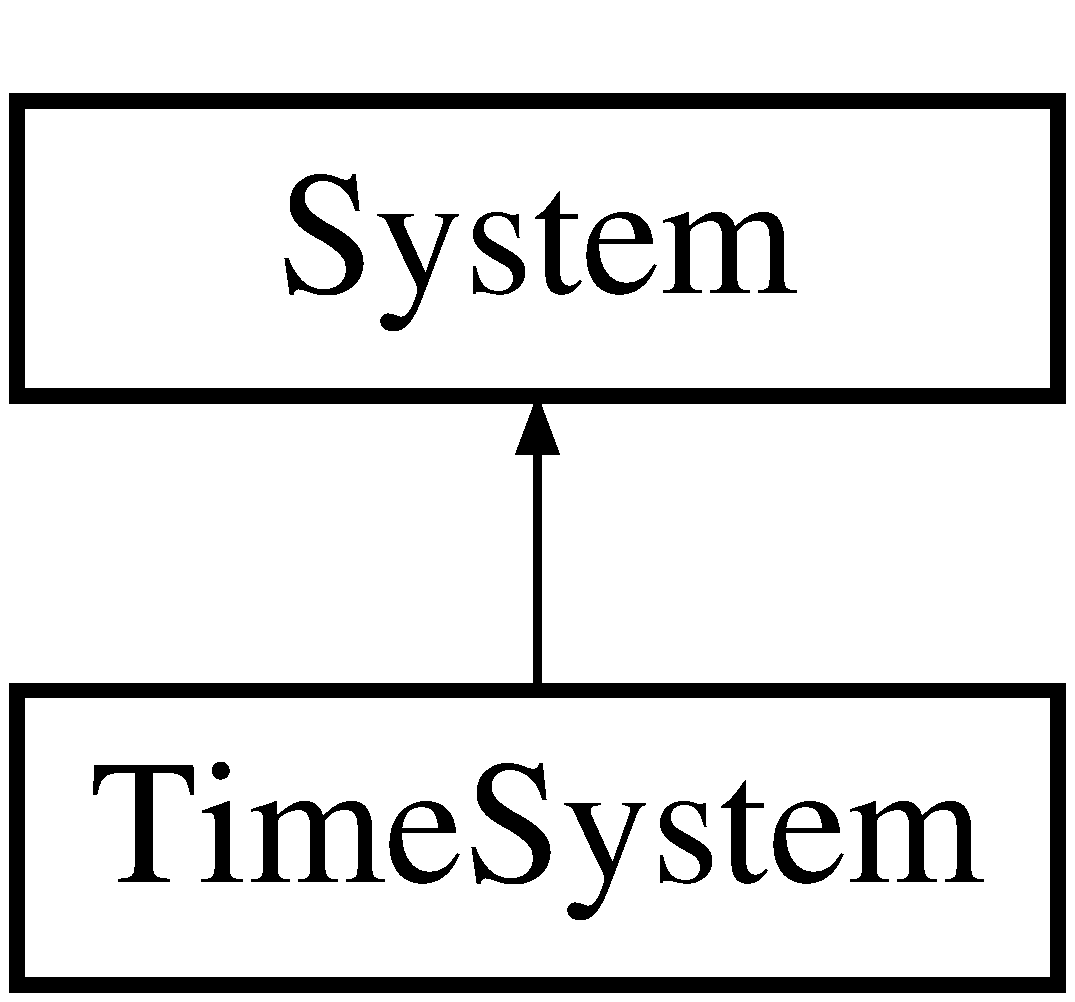
\includegraphics[height=2.000000cm]{class_time_system}
\end{center}
\end{figure}
\subsection*{Public Member Functions}
\begin{DoxyCompactItemize}
\item 
\hyperlink{class_time_system_a2e9142b839e77c2f3bdf5f3c5ff96e8a}{Time\+System} (\hyperlink{class_entity_system}{Entity\+System} \&)
\begin{DoxyCompactList}\small\item\em Constructor. \end{DoxyCompactList}\item 
\hyperlink{class_time_system_a4a0dbfdb6c525380cf71cd781aa0a331}{$\sim$\+Time\+System} ()=default
\begin{DoxyCompactList}\small\item\em Destructor. \end{DoxyCompactList}\item 
void \hyperlink{class_time_system_a628f5adf452ee0a1636ef60d78821293}{update} (tdt\+::real) override
\begin{DoxyCompactList}\small\item\em Updates the time passed for all Time\+Components and handles those that surpassed their target time. \end{DoxyCompactList}\item 
void \hyperlink{class_time_system_a63cd114689c43593a022f370889f28c9}{advance\+\_\+all\+\_\+timers} (tdt\+::real)
\begin{DoxyCompactList}\small\item\em Adds a given time value to all Time\+Components. \end{DoxyCompactList}\item 
void \hyperlink{class_time_system_ae953208be9624a219cfda1baf6dfea8c}{advance\+\_\+all\+\_\+timers\+\_\+of\+\_\+type} (tdt\+::real, T\+I\+M\+E\+\_\+\+E\+V\+E\+NT)
\begin{DoxyCompactList}\small\item\em Adds a given time value to all Time\+Components that match the given time event type. \end{DoxyCompactList}\item 
void \hyperlink{class_time_system_a7baaad1d6985006ed5e247fc9896b6cd}{set\+\_\+time\+\_\+multiplier} (tdt\+::real=1.f)
\begin{DoxyCompactList}\small\item\em Sets the time value by which are all frame times multiplied when added to timers (this allows to slow/speed up all timers). \end{DoxyCompactList}\item 
tdt\+::real \hyperlink{class_time_system_a8f4e42fc4fdbdadcaca49b36a2a181cb}{get\+\_\+time\+\_\+multiplier} ()
\begin{DoxyCompactList}\small\item\em Returns the time value by which are all frame times multiplied when added to timers. \end{DoxyCompactList}\end{DoxyCompactItemize}
\subsection*{Private Member Functions}
\begin{DoxyCompactItemize}
\item 
void \hyperlink{class_time_system_a6020adad2e06402466d59f1ae4209290}{handle\+\_\+event\+\_\+} (tdt\+::uint, \hyperlink{struct_time_component}{Time\+Component} \&)
\begin{DoxyCompactList}\small\item\em Handles a time event when it\textquotesingle{}s timer finnishes. \end{DoxyCompactList}\end{DoxyCompactItemize}
\subsection*{Private Attributes}
\begin{DoxyCompactItemize}
\item 
\hyperlink{class_entity_system}{Entity\+System} \& \hyperlink{class_time_system_abd970f32a5cb10d79d211e0ecdd788a3}{entities\+\_\+}
\begin{DoxyCompactList}\small\item\em Reference to the game\textquotesingle{}s entity system. \end{DoxyCompactList}\item 
tdt\+::real \hyperlink{class_time_system_a4477b8cfae0717af23decf2e90359dad}{time\+\_\+multiplier\+\_\+}
\begin{DoxyCompactList}\small\item\em Allows to speed up all timers. \end{DoxyCompactList}\end{DoxyCompactItemize}


\subsection{Detailed Description}


Definition at line 9 of file Time\+System.\+hpp.



\subsection{Constructor \& Destructor Documentation}
\index{Time\+System@{Time\+System}!Time\+System@{Time\+System}}
\index{Time\+System@{Time\+System}!Time\+System@{Time\+System}}
\subsubsection[{\texorpdfstring{Time\+System(\+Entity\+System \&)}{TimeSystem(EntitySystem &)}}]{\setlength{\rightskip}{0pt plus 5cm}Time\+System\+::\+Time\+System (
\begin{DoxyParamCaption}
\item[{{\bf Entity\+System} \&}]{ents}
\end{DoxyParamCaption}
)}\hypertarget{class_time_system_a2e9142b839e77c2f3bdf5f3c5ff96e8a}{}\label{class_time_system_a2e9142b839e77c2f3bdf5f3c5ff96e8a}


Constructor. 


\begin{DoxyParams}{Parameters}
{\em Reference} & to the game\textquotesingle{}s entity system. \\
\hline
\end{DoxyParams}


Definition at line 7 of file Time\+System.\+cpp.

\index{Time\+System@{Time\+System}!````~Time\+System@{$\sim$\+Time\+System}}
\index{````~Time\+System@{$\sim$\+Time\+System}!Time\+System@{Time\+System}}
\subsubsection[{\texorpdfstring{$\sim$\+Time\+System()=default}{~TimeSystem()=default}}]{\setlength{\rightskip}{0pt plus 5cm}Time\+System\+::$\sim$\+Time\+System (
\begin{DoxyParamCaption}
{}
\end{DoxyParamCaption}
)\hspace{0.3cm}{\ttfamily [default]}}\hypertarget{class_time_system_a4a0dbfdb6c525380cf71cd781aa0a331}{}\label{class_time_system_a4a0dbfdb6c525380cf71cd781aa0a331}


Destructor. 



\subsection{Member Function Documentation}
\index{Time\+System@{Time\+System}!advance\+\_\+all\+\_\+timers@{advance\+\_\+all\+\_\+timers}}
\index{advance\+\_\+all\+\_\+timers@{advance\+\_\+all\+\_\+timers}!Time\+System@{Time\+System}}
\subsubsection[{\texorpdfstring{advance\+\_\+all\+\_\+timers(tdt\+::real)}{advance_all_timers(tdt::real)}}]{\setlength{\rightskip}{0pt plus 5cm}void Time\+System\+::advance\+\_\+all\+\_\+timers (
\begin{DoxyParamCaption}
\item[{tdt\+::real}]{delta}
\end{DoxyParamCaption}
)}\hypertarget{class_time_system_a63cd114689c43593a022f370889f28c9}{}\label{class_time_system_a63cd114689c43593a022f370889f28c9}


Adds a given time value to all Time\+Components. 


\begin{DoxyParams}{Parameters}
{\em Time} & to add. \\
\hline
\end{DoxyParams}


Definition at line 48 of file Time\+System.\+cpp.

\index{Time\+System@{Time\+System}!advance\+\_\+all\+\_\+timers\+\_\+of\+\_\+type@{advance\+\_\+all\+\_\+timers\+\_\+of\+\_\+type}}
\index{advance\+\_\+all\+\_\+timers\+\_\+of\+\_\+type@{advance\+\_\+all\+\_\+timers\+\_\+of\+\_\+type}!Time\+System@{Time\+System}}
\subsubsection[{\texorpdfstring{advance\+\_\+all\+\_\+timers\+\_\+of\+\_\+type(tdt\+::real, T\+I\+M\+E\+\_\+\+E\+V\+E\+N\+T)}{advance_all_timers_of_type(tdt::real, TIME_EVENT)}}]{\setlength{\rightskip}{0pt plus 5cm}void Time\+System\+::advance\+\_\+all\+\_\+timers\+\_\+of\+\_\+type (
\begin{DoxyParamCaption}
\item[{tdt\+::real}]{delta, }
\item[{T\+I\+M\+E\+\_\+\+E\+V\+E\+NT}]{type}
\end{DoxyParamCaption}
)}\hypertarget{class_time_system_ae953208be9624a219cfda1baf6dfea8c}{}\label{class_time_system_ae953208be9624a219cfda1baf6dfea8c}


Adds a given time value to all Time\+Components that match the given time event type. 


\begin{DoxyParams}{Parameters}
{\em Time} & to add. \\
\hline
{\em Time} & even type to match. \\
\hline
\end{DoxyParams}


Definition at line 54 of file Time\+System.\+cpp.

\index{Time\+System@{Time\+System}!get\+\_\+time\+\_\+multiplier@{get\+\_\+time\+\_\+multiplier}}
\index{get\+\_\+time\+\_\+multiplier@{get\+\_\+time\+\_\+multiplier}!Time\+System@{Time\+System}}
\subsubsection[{\texorpdfstring{get\+\_\+time\+\_\+multiplier()}{get_time_multiplier()}}]{\setlength{\rightskip}{0pt plus 5cm}tdt\+::real Time\+System\+::get\+\_\+time\+\_\+multiplier (
\begin{DoxyParamCaption}
{}
\end{DoxyParamCaption}
)}\hypertarget{class_time_system_a8f4e42fc4fdbdadcaca49b36a2a181cb}{}\label{class_time_system_a8f4e42fc4fdbdadcaca49b36a2a181cb}


Returns the time value by which are all frame times multiplied when added to timers. 



Definition at line 68 of file Time\+System.\+cpp.

\index{Time\+System@{Time\+System}!handle\+\_\+event\+\_\+@{handle\+\_\+event\+\_\+}}
\index{handle\+\_\+event\+\_\+@{handle\+\_\+event\+\_\+}!Time\+System@{Time\+System}}
\subsubsection[{\texorpdfstring{handle\+\_\+event\+\_\+(tdt\+::uint, Time\+Component \&)}{handle_event_(tdt::uint, TimeComponent &)}}]{\setlength{\rightskip}{0pt plus 5cm}void Time\+System\+::handle\+\_\+event\+\_\+ (
\begin{DoxyParamCaption}
\item[{tdt\+::uint}]{id, }
\item[{{\bf Time\+Component} \&}]{comp}
\end{DoxyParamCaption}
)\hspace{0.3cm}{\ttfamily [private]}}\hypertarget{class_time_system_a6020adad2e06402466d59f1ae4209290}{}\label{class_time_system_a6020adad2e06402466d59f1ae4209290}


Handles a time event when it\textquotesingle{}s timer finnishes. 


\begin{DoxyParams}{Parameters}
{\em ID} & of the time event. \\
\hline
{\em Reference} & to the \hyperlink{struct_time_component}{Time\+Component} of this time event. \\
\hline
\end{DoxyParams}


Definition at line 73 of file Time\+System.\+cpp.

\index{Time\+System@{Time\+System}!set\+\_\+time\+\_\+multiplier@{set\+\_\+time\+\_\+multiplier}}
\index{set\+\_\+time\+\_\+multiplier@{set\+\_\+time\+\_\+multiplier}!Time\+System@{Time\+System}}
\subsubsection[{\texorpdfstring{set\+\_\+time\+\_\+multiplier(tdt\+::real=1.\+f)}{set_time_multiplier(tdt::real=1.f)}}]{\setlength{\rightskip}{0pt plus 5cm}void Time\+System\+::set\+\_\+time\+\_\+multiplier (
\begin{DoxyParamCaption}
\item[{tdt\+::real}]{val = {\ttfamily 1.f}}
\end{DoxyParamCaption}
)}\hypertarget{class_time_system_a7baaad1d6985006ed5e247fc9896b6cd}{}\label{class_time_system_a7baaad1d6985006ed5e247fc9896b6cd}


Sets the time value by which are all frame times multiplied when added to timers (this allows to slow/speed up all timers). 


\begin{DoxyParams}{Parameters}
{\em The} & new time multiplier. \\
\hline
\end{DoxyParams}


Definition at line 63 of file Time\+System.\+cpp.

\index{Time\+System@{Time\+System}!update@{update}}
\index{update@{update}!Time\+System@{Time\+System}}
\subsubsection[{\texorpdfstring{update(tdt\+::real) override}{update(tdt::real) override}}]{\setlength{\rightskip}{0pt plus 5cm}void Time\+System\+::update (
\begin{DoxyParamCaption}
\item[{tdt\+::real}]{delta}
\end{DoxyParamCaption}
)\hspace{0.3cm}{\ttfamily [override]}, {\ttfamily [virtual]}}\hypertarget{class_time_system_a628f5adf452ee0a1636ef60d78821293}{}\label{class_time_system_a628f5adf452ee0a1636ef60d78821293}


Updates the time passed for all Time\+Components and handles those that surpassed their target time. 


\begin{DoxyParams}{Parameters}
{\em Time} & since last frame. \\
\hline
\end{DoxyParams}


Implements \hyperlink{class_system_a6d54c9bd38eb43d620a1451cb0925472}{System}.



Definition at line 11 of file Time\+System.\+cpp.



\subsection{Member Data Documentation}
\index{Time\+System@{Time\+System}!entities\+\_\+@{entities\+\_\+}}
\index{entities\+\_\+@{entities\+\_\+}!Time\+System@{Time\+System}}
\subsubsection[{\texorpdfstring{entities\+\_\+}{entities_}}]{\setlength{\rightskip}{0pt plus 5cm}{\bf Entity\+System}\& Time\+System\+::entities\+\_\+\hspace{0.3cm}{\ttfamily [private]}}\hypertarget{class_time_system_abd970f32a5cb10d79d211e0ecdd788a3}{}\label{class_time_system_abd970f32a5cb10d79d211e0ecdd788a3}


Reference to the game\textquotesingle{}s entity system. 



Definition at line 68 of file Time\+System.\+hpp.

\index{Time\+System@{Time\+System}!time\+\_\+multiplier\+\_\+@{time\+\_\+multiplier\+\_\+}}
\index{time\+\_\+multiplier\+\_\+@{time\+\_\+multiplier\+\_\+}!Time\+System@{Time\+System}}
\subsubsection[{\texorpdfstring{time\+\_\+multiplier\+\_\+}{time_multiplier_}}]{\setlength{\rightskip}{0pt plus 5cm}tdt\+::real Time\+System\+::time\+\_\+multiplier\+\_\+\hspace{0.3cm}{\ttfamily [private]}}\hypertarget{class_time_system_a4477b8cfae0717af23decf2e90359dad}{}\label{class_time_system_a4477b8cfae0717af23decf2e90359dad}


Allows to speed up all timers. 



Definition at line 73 of file Time\+System.\+hpp.



The documentation for this class was generated from the following files\+:\begin{DoxyCompactItemize}
\item 
systems/Time\+System.\+hpp\item 
systems/Time\+System.\+cpp\end{DoxyCompactItemize}

\hypertarget{class_top_bar}{}\section{Top\+Bar Class Reference}
\label{class_top_bar}\index{Top\+Bar@{Top\+Bar}}


Class representing an info bar on the top of the screen displaying the name of the game, player\textquotesingle{}s gold, mana, units and the current time.  




{\ttfamily \#include $<$Top\+Bar.\+hpp$>$}

Inheritance diagram for Top\+Bar\+:\begin{figure}[H]
\begin{center}
\leavevmode
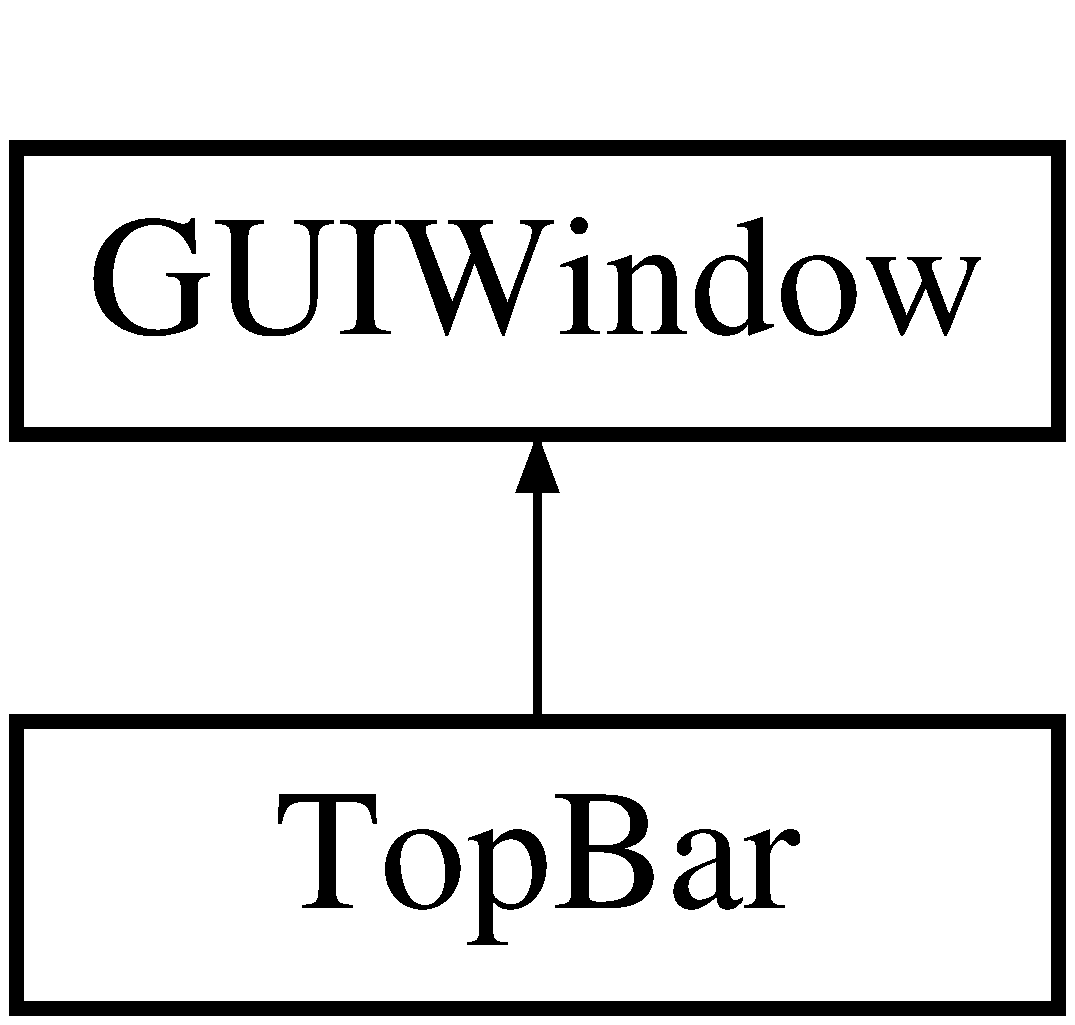
\includegraphics[height=2.000000cm]{class_top_bar}
\end{center}
\end{figure}
\subsection*{Public Member Functions}
\begin{DoxyCompactItemize}
\item 
\hyperlink{class_top_bar_a63a533082a600995f786866cc49b1430}{Top\+Bar} ()
\begin{DoxyCompactList}\small\item\em Constructor. \end{DoxyCompactList}\item 
\hyperlink{class_top_bar_a7094a6ca99beead40e96a29d1a5d0db3}{$\sim$\+Top\+Bar} ()=default
\begin{DoxyCompactList}\small\item\em Destructor. \end{DoxyCompactList}\item 
void \hyperlink{class_top_bar_a8641f2accd0f13d2262669914582cb69}{update\+\_\+time} (tdt\+::real)
\begin{DoxyCompactList}\small\item\em Updates the current time on the top bar if a second passed since the last time update. \end{DoxyCompactList}\item 
void \hyperlink{class_top_bar_a3d83b2b0b1b91e30a275bfb1f7256dba}{update\+\_\+label} (const std\+::string \&, const std\+::string \&)
\begin{DoxyCompactList}\small\item\em Sets the given label\textquotesingle{}s text to the given string. \end{DoxyCompactList}\end{DoxyCompactItemize}
\subsection*{Protected Member Functions}
\begin{DoxyCompactItemize}
\item 
void \hyperlink{class_top_bar_a5e3a678d8c38ee488def54f9d2ce49f0}{init\+\_\+} () override
\begin{DoxyCompactList}\small\item\em Initializes the top bar. \end{DoxyCompactList}\end{DoxyCompactItemize}
\subsection*{Private Attributes}
\begin{DoxyCompactItemize}
\item 
tdt\+::real \hyperlink{class_top_bar_a0b1cc703a118cec101c50ba9b5fccba8}{tdelta\+\_\+}
\begin{DoxyCompactList}\small\item\em Time since the last \char`\"{}\+Current Time\char`\"{} update. \end{DoxyCompactList}\end{DoxyCompactItemize}
\subsection*{Additional Inherited Members}


\subsection{Detailed Description}
Class representing an info bar on the top of the screen displaying the name of the game, player\textquotesingle{}s gold, mana, units and the current time. 

Definition at line 12 of file Top\+Bar.\+hpp.



\subsection{Constructor \& Destructor Documentation}
\index{Top\+Bar@{Top\+Bar}!Top\+Bar@{Top\+Bar}}
\index{Top\+Bar@{Top\+Bar}!Top\+Bar@{Top\+Bar}}
\subsubsection[{\texorpdfstring{Top\+Bar()}{TopBar()}}]{\setlength{\rightskip}{0pt plus 5cm}Top\+Bar\+::\+Top\+Bar (
\begin{DoxyParamCaption}
{}
\end{DoxyParamCaption}
)}\hypertarget{class_top_bar_a63a533082a600995f786866cc49b1430}{}\label{class_top_bar_a63a533082a600995f786866cc49b1430}


Constructor. 



Definition at line 5 of file Top\+Bar.\+cpp.

\index{Top\+Bar@{Top\+Bar}!````~Top\+Bar@{$\sim$\+Top\+Bar}}
\index{````~Top\+Bar@{$\sim$\+Top\+Bar}!Top\+Bar@{Top\+Bar}}
\subsubsection[{\texorpdfstring{$\sim$\+Top\+Bar()=default}{~TopBar()=default}}]{\setlength{\rightskip}{0pt plus 5cm}Top\+Bar\+::$\sim$\+Top\+Bar (
\begin{DoxyParamCaption}
{}
\end{DoxyParamCaption}
)\hspace{0.3cm}{\ttfamily [default]}}\hypertarget{class_top_bar_a7094a6ca99beead40e96a29d1a5d0db3}{}\label{class_top_bar_a7094a6ca99beead40e96a29d1a5d0db3}


Destructor. 



\subsection{Member Function Documentation}
\index{Top\+Bar@{Top\+Bar}!init\+\_\+@{init\+\_\+}}
\index{init\+\_\+@{init\+\_\+}!Top\+Bar@{Top\+Bar}}
\subsubsection[{\texorpdfstring{init\+\_\+() override}{init_() override}}]{\setlength{\rightskip}{0pt plus 5cm}void Top\+Bar\+::init\+\_\+ (
\begin{DoxyParamCaption}
{}
\end{DoxyParamCaption}
)\hspace{0.3cm}{\ttfamily [override]}, {\ttfamily [protected]}, {\ttfamily [virtual]}}\hypertarget{class_top_bar_a5e3a678d8c38ee488def54f9d2ce49f0}{}\label{class_top_bar_a5e3a678d8c38ee488def54f9d2ce49f0}


Initializes the top bar. 



Implements \hyperlink{class_g_u_i_window_a2a7c011363f401a57a26cc7c7652bdfd}{G\+U\+I\+Window}.



Definition at line 28 of file Top\+Bar.\+cpp.

\index{Top\+Bar@{Top\+Bar}!update\+\_\+label@{update\+\_\+label}}
\index{update\+\_\+label@{update\+\_\+label}!Top\+Bar@{Top\+Bar}}
\subsubsection[{\texorpdfstring{update\+\_\+label(const std\+::string \&, const std\+::string \&)}{update_label(const std::string &, const std::string &)}}]{\setlength{\rightskip}{0pt plus 5cm}void Top\+Bar\+::update\+\_\+label (
\begin{DoxyParamCaption}
\item[{const std\+::string \&}]{label, }
\item[{const std\+::string \&}]{val}
\end{DoxyParamCaption}
)}\hypertarget{class_top_bar_a3d83b2b0b1b91e30a275bfb1f7256dba}{}\label{class_top_bar_a3d83b2b0b1b91e30a275bfb1f7256dba}


Sets the given label\textquotesingle{}s text to the given string. 


\begin{DoxyParams}{Parameters}
{\em Label} & to change. \\
\hline
{\em New} & text. \\
\hline
\end{DoxyParams}


Definition at line 23 of file Top\+Bar.\+cpp.

\index{Top\+Bar@{Top\+Bar}!update\+\_\+time@{update\+\_\+time}}
\index{update\+\_\+time@{update\+\_\+time}!Top\+Bar@{Top\+Bar}}
\subsubsection[{\texorpdfstring{update\+\_\+time(tdt\+::real)}{update_time(tdt::real)}}]{\setlength{\rightskip}{0pt plus 5cm}void Top\+Bar\+::update\+\_\+time (
\begin{DoxyParamCaption}
\item[{tdt\+::real}]{delta}
\end{DoxyParamCaption}
)}\hypertarget{class_top_bar_a8641f2accd0f13d2262669914582cb69}{}\label{class_top_bar_a8641f2accd0f13d2262669914582cb69}


Updates the current time on the top bar if a second passed since the last time update. 


\begin{DoxyParams}{Parameters}
{\em Time} & since the last frame. \\
\hline
\end{DoxyParams}


Definition at line 9 of file Top\+Bar.\+cpp.



\subsection{Member Data Documentation}
\index{Top\+Bar@{Top\+Bar}!tdelta\+\_\+@{tdelta\+\_\+}}
\index{tdelta\+\_\+@{tdelta\+\_\+}!Top\+Bar@{Top\+Bar}}
\subsubsection[{\texorpdfstring{tdelta\+\_\+}{tdelta_}}]{\setlength{\rightskip}{0pt plus 5cm}tdt\+::real Top\+Bar\+::tdelta\+\_\+\hspace{0.3cm}{\ttfamily [private]}}\hypertarget{class_top_bar_a0b1cc703a118cec101c50ba9b5fccba8}{}\label{class_top_bar_a0b1cc703a118cec101c50ba9b5fccba8}


Time since the last \char`\"{}\+Current Time\char`\"{} update. 



Definition at line 49 of file Top\+Bar.\+hpp.



The documentation for this class was generated from the following files\+:\begin{DoxyCompactItemize}
\item 
gui/Top\+Bar.\+hpp\item 
gui/Top\+Bar.\+cpp\end{DoxyCompactItemize}

\hypertarget{struct_trigger_component}{}\section{Trigger\+Component Struct Reference}
\label{struct_trigger_component}\index{Trigger\+Component@{Trigger\+Component}}


Allows an entity to cause an effect (by calling it\textquotesingle{}s blueprint) when its triggered (stepped on) or can notify a linked entity which causes the effect.  




{\ttfamily \#include $<$Components.\+hpp$>$}

\subsection*{Public Member Functions}
\begin{DoxyCompactItemize}
\item 
{\bfseries Trigger\+Component} (std\+::string \&\&b=\char`\"{}E\+R\+R\+OR\char`\"{}, tdt\+::real cd=0.f, tdt\+::real rad=0.f)\hypertarget{struct_trigger_component_a78f61e4f767d3bd308627ef10542e46b}{}\label{struct_trigger_component_a78f61e4f767d3bd308627ef10542e46b}

\item 
{\bfseries Trigger\+Component} (const \hyperlink{struct_trigger_component}{Trigger\+Component} \&)=default\hypertarget{struct_trigger_component_a7e972116c79f441d6642935b98dd52d5}{}\label{struct_trigger_component_a7e972116c79f441d6642935b98dd52d5}

\item 
{\bfseries Trigger\+Component} (\hyperlink{struct_trigger_component}{Trigger\+Component} \&\&)=default\hypertarget{struct_trigger_component_a53b7f4db491e1a370bbf1953d0f2de61}{}\label{struct_trigger_component_a53b7f4db491e1a370bbf1953d0f2de61}

\item 
\hyperlink{struct_trigger_component}{Trigger\+Component} \& {\bfseries operator=} (const \hyperlink{struct_trigger_component}{Trigger\+Component} \&)=default\hypertarget{struct_trigger_component_ace8396908728c271c1fb76a4dd0e9910}{}\label{struct_trigger_component_ace8396908728c271c1fb76a4dd0e9910}

\item 
\hyperlink{struct_trigger_component}{Trigger\+Component} \& {\bfseries operator=} (\hyperlink{struct_trigger_component}{Trigger\+Component} \&\&)=default\hypertarget{struct_trigger_component_ad15b8d568aa50e67223914cc4063082c}{}\label{struct_trigger_component_ad15b8d568aa50e67223914cc4063082c}

\end{DoxyCompactItemize}
\subsection*{Public Attributes}
\begin{DoxyCompactItemize}
\item 
std\+::string {\bfseries blueprint}\hypertarget{struct_trigger_component_a81ecf61f5d0b78a090f9f629ca405983}{}\label{struct_trigger_component_a81ecf61f5d0b78a090f9f629ca405983}

\item 
tdt\+::uint {\bfseries linked\+\_\+entity}\hypertarget{struct_trigger_component_abe1d482416c37c036e063c7029c5afbc}{}\label{struct_trigger_component_abe1d482416c37c036e063c7029c5afbc}

\item 
tdt\+::real {\bfseries curr\+\_\+time}\hypertarget{struct_trigger_component_a15eba334acdb1f5ca98980e3f7d4305c}{}\label{struct_trigger_component_a15eba334acdb1f5ca98980e3f7d4305c}

\item 
tdt\+::real {\bfseries cooldown}\hypertarget{struct_trigger_component_a6aca87420677e2246368f579478d70f3}{}\label{struct_trigger_component_a6aca87420677e2246368f579478d70f3}

\item 
tdt\+::real {\bfseries radius}\hypertarget{struct_trigger_component_aaf5f933e332c4e73fa3288f815c454c9}{}\label{struct_trigger_component_aaf5f933e332c4e73fa3288f815c454c9}

\end{DoxyCompactItemize}
\subsection*{Static Public Attributes}
\begin{DoxyCompactItemize}
\item 
static constexpr int {\bfseries type} = 29\hypertarget{struct_trigger_component_a4b40ab020258339d1d28ab3a48e757cc}{}\label{struct_trigger_component_a4b40ab020258339d1d28ab3a48e757cc}

\end{DoxyCompactItemize}


\subsection{Detailed Description}
Allows an entity to cause an effect (by calling it\textquotesingle{}s blueprint) when its triggered (stepped on) or can notify a linked entity which causes the effect. 

Definition at line 689 of file Components.\+hpp.



The documentation for this struct was generated from the following file\+:\begin{DoxyCompactItemize}
\item 
Components.\+hpp\end{DoxyCompactItemize}

\hypertarget{class_trigger_system}{}\section{Trigger\+System Class Reference}
\label{class_trigger_system}\index{Trigger\+System@{Trigger\+System}}


Handles triggers by checking if an entity is standing in their radius when they are off cooldowns.  




{\ttfamily \#include $<$Trigger\+System.\+hpp$>$}

Inheritance diagram for Trigger\+System\+:\begin{figure}[H]
\begin{center}
\leavevmode
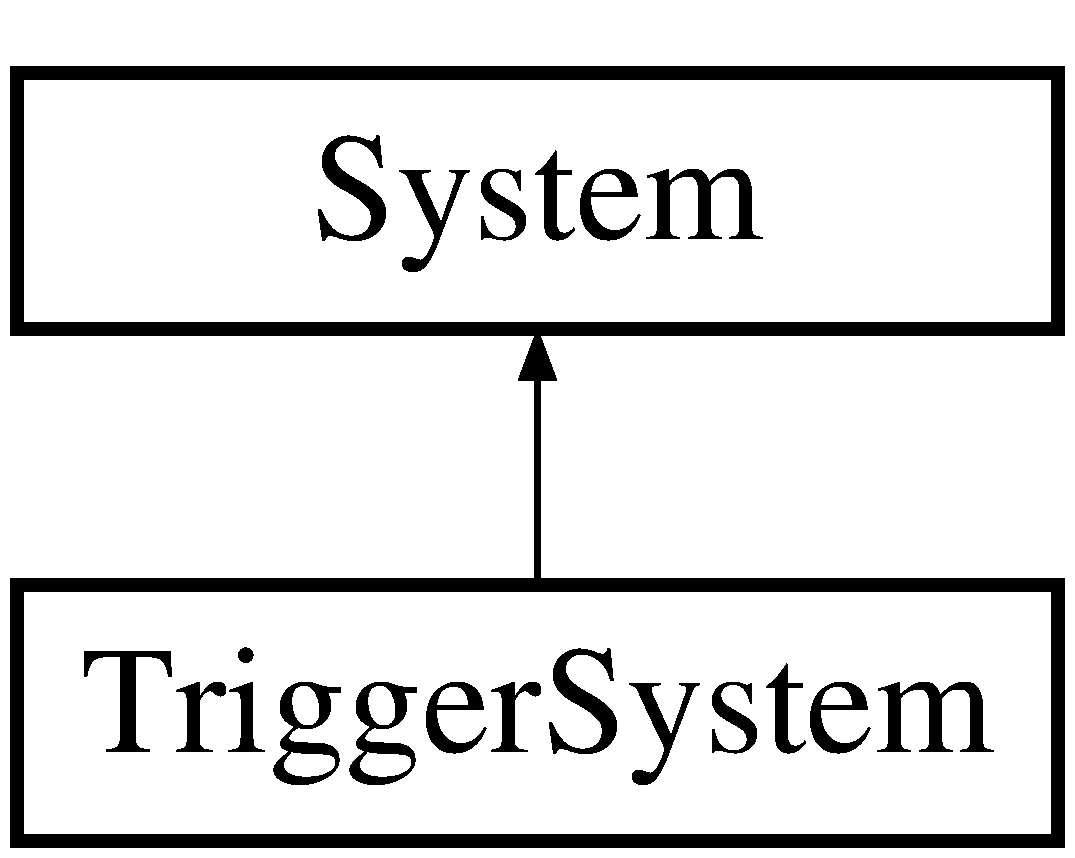
\includegraphics[height=2.000000cm]{class_trigger_system}
\end{center}
\end{figure}
\subsection*{Public Member Functions}
\begin{DoxyCompactItemize}
\item 
\hyperlink{class_trigger_system_ac7e83dc3b48c6f0759834752dd896a99}{Trigger\+System} (\hyperlink{class_entity_system}{Entity\+System} \&)
\begin{DoxyCompactList}\small\item\em Constructor. \end{DoxyCompactList}\item 
\hyperlink{class_trigger_system_a7c897416114b31de2c7371243f6213db}{$\sim$\+Trigger\+System} ()=default
\begin{DoxyCompactList}\small\item\em Destructor. \end{DoxyCompactList}\item 
void \hyperlink{class_trigger_system_ac85976839b1316705e1a493fb40c3ef2}{update} (tdt\+::real) override
\begin{DoxyCompactList}\small\item\em Checks if any entities have been triggered and performs their associated actions if they were. \end{DoxyCompactList}\item 
void \hyperlink{class_trigger_system_a7813aca92f90b5fdf6dd24e9a664a420}{set\+\_\+check\+\_\+period} (tdt\+::real)
\begin{DoxyCompactList}\small\item\em Sets the time period between trigger checks. \end{DoxyCompactList}\item 
tdt\+::real \hyperlink{class_trigger_system_a0161788568894de9f99f362249174b97}{get\+\_\+check\+\_\+period} () const 
\begin{DoxyCompactList}\small\item\em Returns the time period between trigger checks. \end{DoxyCompactList}\end{DoxyCompactItemize}
\subsection*{Private Attributes}
\begin{DoxyCompactItemize}
\item 
\hyperlink{class_entity_system}{Entity\+System} \& \hyperlink{class_trigger_system_a0edd666bdf0821155829c2b3d22b1344}{entities\+\_\+}
\begin{DoxyCompactList}\small\item\em Entity system containing the entities this system works with. \end{DoxyCompactList}\item 
tdt\+::real \hyperlink{class_trigger_system_aba660b6e6bc34da77baa397ffa6d5065}{check\+\_\+timer\+\_\+}
\begin{DoxyCompactList}\small\item\em Allow for dynamic time periods between trigger checks. \end{DoxyCompactList}\item 
tdt\+::real {\bfseries check\+\_\+period\+\_\+}\hypertarget{class_trigger_system_ac46bbc9d22bb38fd16b34cb83bd10157}{}\label{class_trigger_system_ac46bbc9d22bb38fd16b34cb83bd10157}

\end{DoxyCompactItemize}


\subsection{Detailed Description}
Handles triggers by checking if an entity is standing in their radius when they are off cooldowns. 

Definition at line 11 of file Trigger\+System.\+hpp.



\subsection{Constructor \& Destructor Documentation}
\index{Trigger\+System@{Trigger\+System}!Trigger\+System@{Trigger\+System}}
\index{Trigger\+System@{Trigger\+System}!Trigger\+System@{Trigger\+System}}
\subsubsection[{\texorpdfstring{Trigger\+System(\+Entity\+System \&)}{TriggerSystem(EntitySystem &)}}]{\setlength{\rightskip}{0pt plus 5cm}Trigger\+System\+::\+Trigger\+System (
\begin{DoxyParamCaption}
\item[{{\bf Entity\+System} \&}]{ents}
\end{DoxyParamCaption}
)}\hypertarget{class_trigger_system_ac7e83dc3b48c6f0759834752dd896a99}{}\label{class_trigger_system_ac7e83dc3b48c6f0759834752dd896a99}


Constructor. 


\begin{DoxyParams}{Parameters}
{\em Entity} & system containing entities this system works with. \\
\hline
\end{DoxyParams}


Definition at line 6 of file Trigger\+System.\+cpp.

\index{Trigger\+System@{Trigger\+System}!````~Trigger\+System@{$\sim$\+Trigger\+System}}
\index{````~Trigger\+System@{$\sim$\+Trigger\+System}!Trigger\+System@{Trigger\+System}}
\subsubsection[{\texorpdfstring{$\sim$\+Trigger\+System()=default}{~TriggerSystem()=default}}]{\setlength{\rightskip}{0pt plus 5cm}Trigger\+System\+::$\sim$\+Trigger\+System (
\begin{DoxyParamCaption}
{}
\end{DoxyParamCaption}
)\hspace{0.3cm}{\ttfamily [default]}}\hypertarget{class_trigger_system_a7c897416114b31de2c7371243f6213db}{}\label{class_trigger_system_a7c897416114b31de2c7371243f6213db}


Destructor. 



\subsection{Member Function Documentation}
\index{Trigger\+System@{Trigger\+System}!get\+\_\+check\+\_\+period@{get\+\_\+check\+\_\+period}}
\index{get\+\_\+check\+\_\+period@{get\+\_\+check\+\_\+period}!Trigger\+System@{Trigger\+System}}
\subsubsection[{\texorpdfstring{get\+\_\+check\+\_\+period() const }{get_check_period() const }}]{\setlength{\rightskip}{0pt plus 5cm}tdt\+::real Trigger\+System\+::get\+\_\+check\+\_\+period (
\begin{DoxyParamCaption}
{}
\end{DoxyParamCaption}
) const}\hypertarget{class_trigger_system_a0161788568894de9f99f362249174b97}{}\label{class_trigger_system_a0161788568894de9f99f362249174b97}


Returns the time period between trigger checks. 



Definition at line 65 of file Trigger\+System.\+cpp.

\index{Trigger\+System@{Trigger\+System}!set\+\_\+check\+\_\+period@{set\+\_\+check\+\_\+period}}
\index{set\+\_\+check\+\_\+period@{set\+\_\+check\+\_\+period}!Trigger\+System@{Trigger\+System}}
\subsubsection[{\texorpdfstring{set\+\_\+check\+\_\+period(tdt\+::real)}{set_check_period(tdt::real)}}]{\setlength{\rightskip}{0pt plus 5cm}void Trigger\+System\+::set\+\_\+check\+\_\+period (
\begin{DoxyParamCaption}
\item[{tdt\+::real}]{val}
\end{DoxyParamCaption}
)}\hypertarget{class_trigger_system_a7813aca92f90b5fdf6dd24e9a664a420}{}\label{class_trigger_system_a7813aca92f90b5fdf6dd24e9a664a420}


Sets the time period between trigger checks. 


\begin{DoxyParams}{Parameters}
{\em The} & new time period. \\
\hline
\end{DoxyParams}


Definition at line 60 of file Trigger\+System.\+cpp.

\index{Trigger\+System@{Trigger\+System}!update@{update}}
\index{update@{update}!Trigger\+System@{Trigger\+System}}
\subsubsection[{\texorpdfstring{update(tdt\+::real) override}{update(tdt::real) override}}]{\setlength{\rightskip}{0pt plus 5cm}void Trigger\+System\+::update (
\begin{DoxyParamCaption}
\item[{tdt\+::real}]{delta}
\end{DoxyParamCaption}
)\hspace{0.3cm}{\ttfamily [override]}, {\ttfamily [virtual]}}\hypertarget{class_trigger_system_ac85976839b1316705e1a493fb40c3ef2}{}\label{class_trigger_system_ac85976839b1316705e1a493fb40c3ef2}


Checks if any entities have been triggered and performs their associated actions if they were. 


\begin{DoxyParams}{Parameters}
{\em Time} & since the last frame. \\
\hline
\end{DoxyParams}


Implements \hyperlink{class_system_a6d54c9bd38eb43d620a1451cb0925472}{System}.



Definition at line 10 of file Trigger\+System.\+cpp.



\subsection{Member Data Documentation}
\index{Trigger\+System@{Trigger\+System}!check\+\_\+timer\+\_\+@{check\+\_\+timer\+\_\+}}
\index{check\+\_\+timer\+\_\+@{check\+\_\+timer\+\_\+}!Trigger\+System@{Trigger\+System}}
\subsubsection[{\texorpdfstring{check\+\_\+timer\+\_\+}{check_timer_}}]{\setlength{\rightskip}{0pt plus 5cm}tdt\+::real Trigger\+System\+::check\+\_\+timer\+\_\+\hspace{0.3cm}{\ttfamily [private]}}\hypertarget{class_trigger_system_aba660b6e6bc34da77baa397ffa6d5065}{}\label{class_trigger_system_aba660b6e6bc34da77baa397ffa6d5065}


Allow for dynamic time periods between trigger checks. 



Definition at line 53 of file Trigger\+System.\+hpp.

\index{Trigger\+System@{Trigger\+System}!entities\+\_\+@{entities\+\_\+}}
\index{entities\+\_\+@{entities\+\_\+}!Trigger\+System@{Trigger\+System}}
\subsubsection[{\texorpdfstring{entities\+\_\+}{entities_}}]{\setlength{\rightskip}{0pt plus 5cm}{\bf Entity\+System}\& Trigger\+System\+::entities\+\_\+\hspace{0.3cm}{\ttfamily [private]}}\hypertarget{class_trigger_system_a0edd666bdf0821155829c2b3d22b1344}{}\label{class_trigger_system_a0edd666bdf0821155829c2b3d22b1344}


Entity system containing the entities this system works with. 



Definition at line 48 of file Trigger\+System.\+hpp.



The documentation for this class was generated from the following files\+:\begin{DoxyCompactItemize}
\item 
systems/Trigger\+System.\+hpp\item 
systems/Trigger\+System.\+cpp\end{DoxyCompactItemize}

\hypertarget{struct_upgrade_component}{}\section{Upgrade\+Component Struct Reference}
\label{struct_upgrade_component}\index{Upgrade\+Component@{Upgrade\+Component}}


Represents the game\textquotesingle{}s leveling system component, contains info about experience and leveling progression as well as the blueprint that gets called on level up.  




{\ttfamily \#include $<$Components.\+hpp$>$}

\subsection*{Public Member Functions}
\begin{DoxyCompactItemize}
\item 
{\bfseries Upgrade\+Component} (std\+::string \&\&b=\char`\"{}E\+R\+R\+OR\char`\"{}, tdt\+::uint exp=100, tdt\+::uint cap=5)\hypertarget{struct_upgrade_component_a69af5ff48cb7ec6ce960e6d80289ba85}{}\label{struct_upgrade_component_a69af5ff48cb7ec6ce960e6d80289ba85}

\item 
{\bfseries Upgrade\+Component} (const \hyperlink{struct_upgrade_component}{Upgrade\+Component} \&)=default\hypertarget{struct_upgrade_component_a140db550d9998fb3244e95d59b8221b8}{}\label{struct_upgrade_component_a140db550d9998fb3244e95d59b8221b8}

\item 
{\bfseries Upgrade\+Component} (\hyperlink{struct_upgrade_component}{Upgrade\+Component} \&\&)=default\hypertarget{struct_upgrade_component_abeb73cb8e09b4246e0d7db65a6269e0d}{}\label{struct_upgrade_component_abeb73cb8e09b4246e0d7db65a6269e0d}

\item 
\hyperlink{struct_upgrade_component}{Upgrade\+Component} \& {\bfseries operator=} (const \hyperlink{struct_upgrade_component}{Upgrade\+Component} \&)=default\hypertarget{struct_upgrade_component_a618a2eb7310699f380607c75da212b4a}{}\label{struct_upgrade_component_a618a2eb7310699f380607c75da212b4a}

\item 
\hyperlink{struct_upgrade_component}{Upgrade\+Component} \& {\bfseries operator=} (\hyperlink{struct_upgrade_component}{Upgrade\+Component} \&\&)=default\hypertarget{struct_upgrade_component_af47647e904ffcf6483c61c3447d41bc4}{}\label{struct_upgrade_component_af47647e904ffcf6483c61c3447d41bc4}

\end{DoxyCompactItemize}
\subsection*{Public Attributes}
\begin{DoxyCompactItemize}
\item 
std\+::string {\bfseries blueprint}\hypertarget{struct_upgrade_component_a1c8235c9cd5adb1404edf5a4649f363e}{}\label{struct_upgrade_component_a1c8235c9cd5adb1404edf5a4649f363e}

\item 
tdt\+::uint {\bfseries experience}\hypertarget{struct_upgrade_component_a3c3b93a56ba521102d671b78c0ca4f34}{}\label{struct_upgrade_component_a3c3b93a56ba521102d671b78c0ca4f34}

\item 
tdt\+::uint {\bfseries exp\+\_\+needed}\hypertarget{struct_upgrade_component_ab7c4f3c857e3d3a50b744087de98854d}{}\label{struct_upgrade_component_ab7c4f3c857e3d3a50b744087de98854d}

\item 
tdt\+::uint {\bfseries level}\hypertarget{struct_upgrade_component_a1efa01000f6bbe592174640a98da2d77}{}\label{struct_upgrade_component_a1efa01000f6bbe592174640a98da2d77}

\item 
tdt\+::uint {\bfseries level\+\_\+cap}\hypertarget{struct_upgrade_component_ab4e7fd44247ca15360e9dd58fd7ddd14}{}\label{struct_upgrade_component_ab4e7fd44247ca15360e9dd58fd7ddd14}

\end{DoxyCompactItemize}
\subsection*{Static Public Attributes}
\begin{DoxyCompactItemize}
\item 
static constexpr int {\bfseries type} = 30\hypertarget{struct_upgrade_component_a2f60d71c1d1e255be9996289ddb8c119}{}\label{struct_upgrade_component_a2f60d71c1d1e255be9996289ddb8c119}

\end{DoxyCompactItemize}


\subsection{Detailed Description}
Represents the game\textquotesingle{}s leveling system component, contains info about experience and leveling progression as well as the blueprint that gets called on level up. 

Definition at line 714 of file Components.\+hpp.



The documentation for this struct was generated from the following file\+:\begin{DoxyCompactItemize}
\item 
Components.\+hpp\end{DoxyCompactItemize}

\hypertarget{class_wave_system}{}\section{Wave\+System Class Reference}
\label{class_wave_system}\index{Wave\+System@{Wave\+System}}


This system creates the entities attacking the player\textquotesingle{}s dungeon in a similar fashion to tower defense games.  




{\ttfamily \#include $<$Wave\+System.\+hpp$>$}

Inheritance diagram for Wave\+System\+:\begin{figure}[H]
\begin{center}
\leavevmode
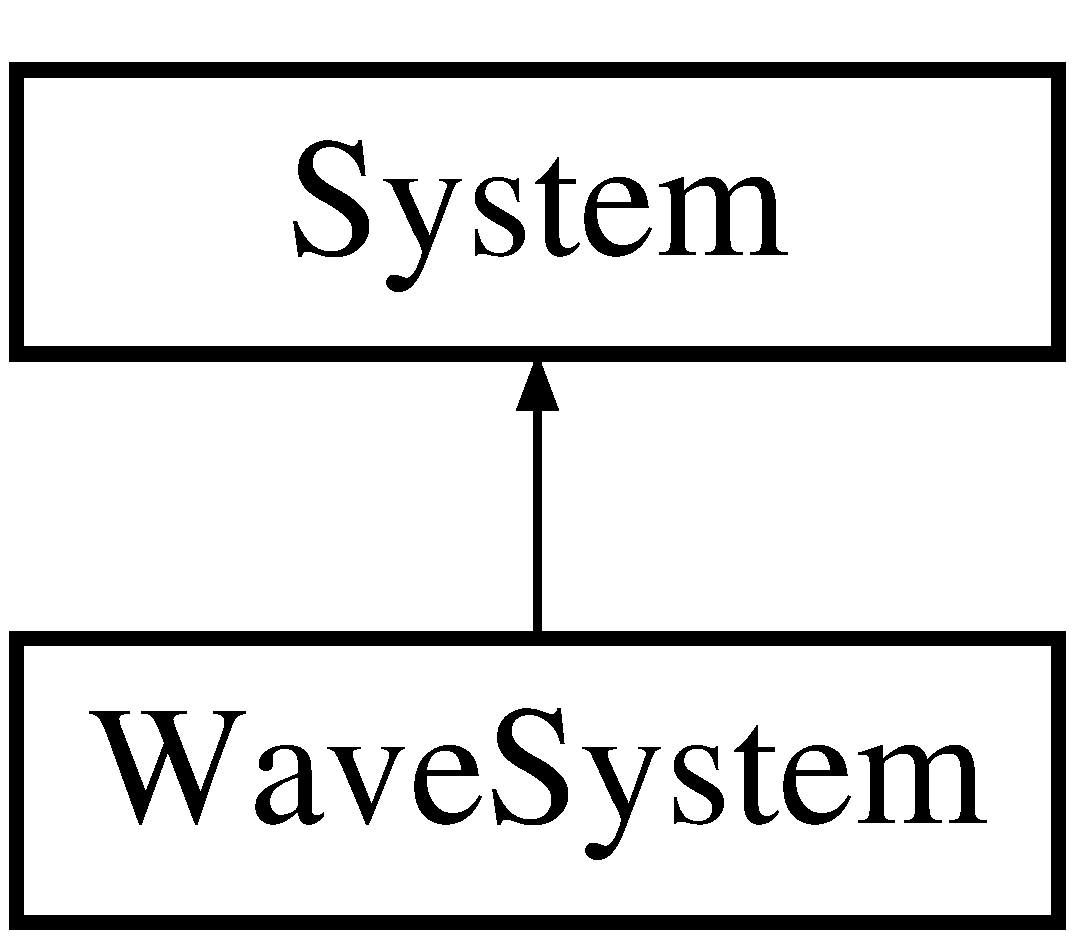
\includegraphics[height=2.000000cm]{class_wave_system}
\end{center}
\end{figure}
\subsection*{Public Member Functions}
\begin{DoxyCompactItemize}
\item 
\hyperlink{class_wave_system_a29290eac1f7d107ca891e9ee08192630}{Wave\+System} (\hyperlink{class_entity_system}{Entity\+System} \&)
\begin{DoxyCompactList}\small\item\em Constructor. \end{DoxyCompactList}\item 
\hyperlink{class_wave_system_aef0ccfc8165a323ef94c38e707de7eb2}{$\sim$\+Wave\+System} ()=default
\begin{DoxyCompactList}\small\item\em Destructor. \end{DoxyCompactList}\item 
void \hyperlink{class_wave_system_a98df4388628f2618db5c2aa18ce67c11}{update} (tdt\+::real) override
\begin{DoxyCompactList}\small\item\em Updates all necessary timers and checks if a wave has arrived and if so, spawns it. \end{DoxyCompactList}\item 
void \hyperlink{class_wave_system_ae145f693f33074fb68273d23bb9fd36c}{set\+\_\+countdown\+\_\+window} (C\+E\+G\+U\+I\+::\+Window $\ast$)
\begin{DoxyCompactList}\small\item\em Saves pointer to the window that is used to show the countdown to the next wave. \end{DoxyCompactList}\item 
void \hyperlink{class_wave_system_a8ac386c12cc0458e7faf05dcc96da02b}{next\+\_\+wave} ()
\begin{DoxyCompactList}\small\item\em Finnishes the wave countdown, causing a wave to be spawned on the next update call. \end{DoxyCompactList}\item 
void \hyperlink{class_wave_system_aab24fdbbbfb06ac094a5cc54d221a9fd}{advance\+\_\+wave\+\_\+countdown} (tdt\+::uint)
\begin{DoxyCompactList}\small\item\em Advances the countdown by a given amount of time. \end{DoxyCompactList}\item 
void \hyperlink{class_wave_system_aa14e5872f96047435b548954fbabdcd6}{wave\+\_\+entity\+\_\+died} ()
\begin{DoxyCompactList}\small\item\em Registers a death of an entity that belongs to the current wave (called by it\textquotesingle{}s destructor). \end{DoxyCompactList}\item 
void \hyperlink{class_wave_system_a89b2ca21abdcb03249b30f11e07bedaa}{start} ()
\begin{DoxyCompactList}\small\item\em Starts (and initializes) the wave system. \end{DoxyCompactList}\item 
void \hyperlink{class_wave_system_a4e92e26fc773d507bf7cb7d75d4c4ddd}{pause} (bool)
\begin{DoxyCompactList}\small\item\em Changes the state of the system. \end{DoxyCompactList}\item 
void \hyperlink{class_wave_system_a4ed4f0b470bbeff062535a7a7b0d26a5}{set\+\_\+entity\+\_\+total} (tdt\+::uint)
\begin{DoxyCompactList}\small\item\em Sets the total number of entities the wave is gonna have. \end{DoxyCompactList}\item 
tdt\+::uint \hyperlink{class_wave_system_aa563d934ce6552ff5184d8deadd1a2c2}{get\+\_\+entity\+\_\+total} () const 
\begin{DoxyCompactList}\small\item\em Returns the total number of entities the wave is gonna have. \end{DoxyCompactList}\item 
void \hyperlink{class_wave_system_a78d88369731c166b2769bde431593e08}{set\+\_\+wave\+\_\+count} (tdt\+::uint)
\begin{DoxyCompactList}\small\item\em Sets the number of waves before the system stops. \end{DoxyCompactList}\item 
tdt\+::uint \hyperlink{class_wave_system_af0ca06c6dda78b2ad0a85ce71f3c60a3}{get\+\_\+wave\+\_\+count} () const 
\begin{DoxyCompactList}\small\item\em Returns the total number of waves the system has. \end{DoxyCompactList}\item 
void \hyperlink{class_wave_system_a50b83a5cd977a4f834044b7613bfc3d2}{add\+\_\+spawn\+\_\+node} (tdt\+::uint)
\begin{DoxyCompactList}\small\item\em Adds a grid node to the spawn list. \end{DoxyCompactList}\item 
void \hyperlink{class_wave_system_ab818eaa3d2058bb1f6c1cf917ffb6dec}{clear\+\_\+spawn\+\_\+nodes} ()
\begin{DoxyCompactList}\small\item\em Removes any registered spawn nodes. \end{DoxyCompactList}\item 
void \hyperlink{class_wave_system_acd6966753dd5d2e99d7c29069308c38b}{set\+\_\+spawn\+\_\+cooldown} (tdt\+::real)
\begin{DoxyCompactList}\small\item\em Sets the delay between spawns (if \# of spawn nodes is smaller than \# of wave entities). \end{DoxyCompactList}\item 
tdt\+::real \hyperlink{class_wave_system_a9496f6b821617e2554634c5866ea0be6}{get\+\_\+spawn\+\_\+cooldown} () const 
\begin{DoxyCompactList}\small\item\em Returns the delay between spawns. \end{DoxyCompactList}\item 
void \hyperlink{class_wave_system_a619c6572a4926d37af744d382be38bef}{update\+\_\+label\+\_\+text} ()
\begin{DoxyCompactList}\small\item\em Updates the countdown window\textquotesingle{}s text. \end{DoxyCompactList}\item 
void \hyperlink{class_wave_system_af231cca40f1e32e3fa4f9f38b92a760d}{add\+\_\+entity\+\_\+blueprint} (const std\+::string \&)
\begin{DoxyCompactList}\small\item\em Adds a blueprint table for a new wave entity. \end{DoxyCompactList}\item 
const std\+::vector$<$ std\+::string $>$ \& \hyperlink{class_wave_system_a9f7d4f3574df6e75384d0eef48d8a011}{get\+\_\+entity\+\_\+blueprints} () const 
\begin{DoxyCompactList}\small\item\em Returns a vector of all entities in the wave. \end{DoxyCompactList}\item 
void \hyperlink{class_wave_system_ab983f35629a29a6b7fe407001c14b0be}{set\+\_\+wave\+\_\+table} (const std\+::string \&)
\begin{DoxyCompactList}\small\item\em Sets the table this system is using to create waves. \end{DoxyCompactList}\item 
const std\+::string \& \hyperlink{class_wave_system_aa5d62ed61dc416829d052f225eb8f4a7}{get\+\_\+wave\+\_\+table} () const 
\begin{DoxyCompactList}\small\item\em Returns the table this system is using to create waves. \end{DoxyCompactList}\item 
const std\+::vector$<$ tdt\+::uint $>$ \& \hyperlink{class_wave_system_a22da39953a79e71915e15c2515b07550}{get\+\_\+spawning\+\_\+nodes} () const 
\begin{DoxyCompactList}\small\item\em Returns a vector of nodes that are marked as spawners for the wave. \end{DoxyCompactList}\item 
void \hyperlink{class_wave_system_a91988914db2f2d6bf3ce4e6efbc6c00a}{set\+\_\+curr\+\_\+wave\+\_\+number} (tdt\+::uint)
\begin{DoxyCompactList}\small\item\em Sets the number of the current wave. \end{DoxyCompactList}\item 
tdt\+::uint \hyperlink{class_wave_system_a7bf5631871f34d83341b5ec881906ba7}{get\+\_\+curr\+\_\+wave\+\_\+number} () const 
\begin{DoxyCompactList}\small\item\em Returns the number of the current wave. \end{DoxyCompactList}\item 
void \hyperlink{class_wave_system_aa02519f3d7c79a5d020ceaf7ad82b341}{set\+\_\+countdown\+\_\+value} (tdt\+::uint)
\begin{DoxyCompactList}\small\item\em Sets the time remaining before the next wave. \end{DoxyCompactList}\item 
tdt\+::uint \hyperlink{class_wave_system_af667048a9cd9373137eaef4837eb344e}{get\+\_\+countdown\+\_\+value} () const 
\begin{DoxyCompactList}\small\item\em Returns the time remaining before the next wave. \end{DoxyCompactList}\item 
void \hyperlink{class_wave_system_a3431e72c157cc75d1ad720b2992fe563}{set\+\_\+state} (W\+A\+V\+E\+\_\+\+S\+T\+A\+TE)
\begin{DoxyCompactList}\small\item\em Changes the state of the wave system. \end{DoxyCompactList}\item 
W\+A\+V\+E\+\_\+\+S\+T\+A\+TE \hyperlink{class_wave_system_a82da4bcf0e5afd20c2ae984234b4679d}{get\+\_\+state} () const 
\begin{DoxyCompactList}\small\item\em Returns the state of the wave system. \end{DoxyCompactList}\item 
void \hyperlink{class_wave_system_a3980c6abc389500169aa32932e300e46}{set\+\_\+spawn\+\_\+timer} (tdt\+::real)
\begin{DoxyCompactList}\small\item\em Sets the time on the spawn timer, which causes the next spawn batch to appear when it reaches the spawn cooldown value. \end{DoxyCompactList}\item 
tdt\+::real \hyperlink{class_wave_system_a70f7ec41e60ce75caffd2fd98e627d28}{get\+\_\+spawn\+\_\+timer} () const 
\begin{DoxyCompactList}\small\item\em Returns the time on the spawn timer, which causes the next spawn batch to appear when it reaches the spawn cooldown value. \end{DoxyCompactList}\item 
void \hyperlink{class_wave_system_ac359a846058fb5f45e34eca64438dfc9}{set\+\_\+wave\+\_\+entities} (tdt\+::uint)
\begin{DoxyCompactList}\small\item\em Sets the number of entities the current wave has alive. \end{DoxyCompactList}\item 
tdt\+::uint \hyperlink{class_wave_system_a6e446d9424066896680103a7c2a22c06}{get\+\_\+wave\+\_\+entities} () const 
\begin{DoxyCompactList}\small\item\em Returns the number of entities the current wave has alive. \end{DoxyCompactList}\item 
void \hyperlink{class_wave_system_a54052c43df7a6e7be869b705c27641c7}{set\+\_\+entities\+\_\+spawned} (tdt\+::uint)
\begin{DoxyCompactList}\small\item\em Sets the number of entities already spawned in this wave. \end{DoxyCompactList}\item 
tdt\+::uint \hyperlink{class_wave_system_a5ba8e7f51331db297c3fb8ff317021eb}{get\+\_\+entities\+\_\+spawned} () const 
\begin{DoxyCompactList}\small\item\em Returns the number of entities already spawned in this wave. \end{DoxyCompactList}\item 
void \hyperlink{class_wave_system_a64ee44c82e52e02ac332608a1f54febc}{clear\+\_\+entity\+\_\+blueprints} ()
\begin{DoxyCompactList}\small\item\em Clears any entity blueprints that were gonna be used in the next wave. \end{DoxyCompactList}\item 
void \hyperlink{class_wave_system_a6068d7406fbaf4a2aa18e1b5e13a79a7}{set\+\_\+endless\+\_\+mode} (bool)
\begin{DoxyCompactList}\small\item\em Sets the endless flag (true -\/$>$ last wave repeats). \end{DoxyCompactList}\item 
bool \hyperlink{class_wave_system_ab12aad00426af3a0b67d6ff2c6387b47}{get\+\_\+endless\+\_\+mode} () const 
\begin{DoxyCompactList}\small\item\em Returns the endless flag (true -\/$>$ last wave repeats). \end{DoxyCompactList}\end{DoxyCompactItemize}
\subsection*{Private Member Functions}
\begin{DoxyCompactItemize}
\item 
void \hyperlink{class_wave_system_afa2eb918f42c322630c5ed1f0c3d3355}{start\+\_\+wave} ()
\begin{DoxyCompactList}\small\item\em Starts the current wave. \end{DoxyCompactList}\item 
void \hyperlink{class_wave_system_a1f600d9b4fb4646bef2aa2dccc8809ac}{end\+\_\+wave} ()
\begin{DoxyCompactList}\small\item\em Ends the current wave. \end{DoxyCompactList}\item 
void \hyperlink{class_wave_system_af0a6a8cbcc4663d5ada8b6dd7d77b972}{spawn} ()
\begin{DoxyCompactList}\small\item\em Spawns the next batch of entities. \end{DoxyCompactList}\end{DoxyCompactItemize}
\subsection*{Private Attributes}
\begin{DoxyCompactItemize}
\item 
W\+A\+V\+E\+\_\+\+S\+T\+A\+TE \hyperlink{class_wave_system_add90dfd41a5917d398623fcea26fb269}{state\+\_\+}
\begin{DoxyCompactList}\small\item\em The current state of the system. \end{DoxyCompactList}\item 
\hyperlink{class_entity_system}{Entity\+System} \& \hyperlink{class_wave_system_a8f590c5b9cf0cd5f7fdc5afee19dd389}{entities\+\_\+}
\begin{DoxyCompactList}\small\item\em Entity system in which the wave entities will be created. \end{DoxyCompactList}\item 
tdt\+::uint \hyperlink{class_wave_system_a10aa7985fe118508460c7c9498c94a69}{curr\+\_\+wave\+\_\+number\+\_\+}
\begin{DoxyCompactList}\small\item\em Number of the current wave. \end{DoxyCompactList}\item 
tdt\+::uint \hyperlink{class_wave_system_af0ea0ae6d2397d9cb0d69cd19eca3177}{wave\+\_\+count\+\_\+}
\begin{DoxyCompactList}\small\item\em Total number of waves. \end{DoxyCompactList}\item 
tdt\+::uint \hyperlink{class_wave_system_a378035c7325464436bce4235678dfe42}{wave\+\_\+entities\+\_\+}
\begin{DoxyCompactList}\small\item\em Number of entities in the current wave that are spawned and still alive. \end{DoxyCompactList}\item 
tdt\+::uint \hyperlink{class_wave_system_ab25df374df710d5fca47d39a39859f66}{entities\+\_\+spawned\+\_\+}
\begin{DoxyCompactList}\small\item\em Number of entities that were already spawned during this wave. \end{DoxyCompactList}\item 
tdt\+::uint \hyperlink{class_wave_system_a222d726e4ea7d49ffe856c5ded840938}{entities\+\_\+total\+\_\+}
\begin{DoxyCompactList}\small\item\em Total number of entities in the current wave. \end{DoxyCompactList}\item 
tdt\+::uint \hyperlink{class_wave_system_ae70ca36a66a8df6d356539c7e0cc0e19}{next\+\_\+wave\+\_\+countdown\+\_\+}
\begin{DoxyCompactList}\small\item\em Time in seconds till the next wave starts. \end{DoxyCompactList}\item 
tdt\+::real \hyperlink{class_wave_system_a9d249d2778d8f7a618274bcc6b8ed3aa}{second\+\_\+timer\+\_\+}
\begin{DoxyCompactList}\small\item\em Auxiliary timer that is used to measure seconds. \end{DoxyCompactList}\item 
std\+::string \hyperlink{class_wave_system_a1c1cc583c1285417a68295bed7272fe3}{label\+\_\+text\+\_\+}
\begin{DoxyCompactList}\small\item\em Text that is displayed in the countdown window. \end{DoxyCompactList}\item 
C\+E\+G\+U\+I\+::\+Window $\ast$ \hyperlink{class_wave_system_ab945c8a6f6608420128bc1e0c101cb09}{window\+\_\+}
\begin{DoxyCompactList}\small\item\em Pointer to the countdown window. \end{DoxyCompactList}\item 
\hyperlink{classlpp_1_1_script}{lpp\+::\+Script} \& \hyperlink{class_wave_system_a0a4f867a7e8179bb77235e4d66bdc67e}{script\+\_\+}
\begin{DoxyCompactList}\small\item\em Reference to the script engine for easier use. \end{DoxyCompactList}\item 
std\+::vector$<$ tdt\+::uint $>$ \hyperlink{class_wave_system_a28ea2af56b6debb00a1fd780b8ace530}{spawning\+\_\+nodes\+\_\+}
\begin{DoxyCompactList}\small\item\em Nodes that are used for entity spawning. \end{DoxyCompactList}\item 
tdt\+::real \hyperlink{class_wave_system_ada44d4ac39d896951051bb1e983a0f1b}{spawn\+\_\+timer\+\_\+}
\begin{DoxyCompactList}\small\item\em Timers used for entity spawning. \end{DoxyCompactList}\item 
tdt\+::real {\bfseries spawn\+\_\+cooldown\+\_\+}\hypertarget{class_wave_system_aa13206e3d5916cfb9062adec8cb99bcd}{}\label{class_wave_system_aa13206e3d5916cfb9062adec8cb99bcd}

\item 
std\+::string \hyperlink{class_wave_system_a98c198bf1c005e3861c22c28eee0f791}{wave\+\_\+table\+\_\+}
\begin{DoxyCompactList}\small\item\em Name of the table containing init, wstart and wend functions that define a wave system. \end{DoxyCompactList}\item 
std\+::vector$<$ std\+::string $>$ \hyperlink{class_wave_system_a454da77779387bb1f4da83a22880b061}{entity\+\_\+blueprints\+\_\+}
\begin{DoxyCompactList}\small\item\em Entities that are gonna be spawned. \end{DoxyCompactList}\item 
bool \hyperlink{class_wave_system_a9d79eb962ae15b6b77517f5f9a4b16a6}{endless\+\_\+mode\+\_\+}
\begin{DoxyCompactList}\small\item\em If true, the current wave keeps repeating. \end{DoxyCompactList}\end{DoxyCompactItemize}


\subsection{Detailed Description}
This system creates the entities attacking the player\textquotesingle{}s dungeon in a similar fashion to tower defense games. 

\begin{DoxyNote}{Note}
This systems contains a large number of setters/getters (while most of other systems do not). This is because this system has to be fully serialized when saving the game to save the game\textquotesingle{}s progress. 
\end{DoxyNote}


Definition at line 25 of file Wave\+System.\+hpp.



\subsection{Constructor \& Destructor Documentation}
\index{Wave\+System@{Wave\+System}!Wave\+System@{Wave\+System}}
\index{Wave\+System@{Wave\+System}!Wave\+System@{Wave\+System}}
\subsubsection[{\texorpdfstring{Wave\+System(\+Entity\+System \&)}{WaveSystem(EntitySystem &)}}]{\setlength{\rightskip}{0pt plus 5cm}Wave\+System\+::\+Wave\+System (
\begin{DoxyParamCaption}
\item[{{\bf Entity\+System} \&}]{ents}
\end{DoxyParamCaption}
)}\hypertarget{class_wave_system_a29290eac1f7d107ca891e9ee08192630}{}\label{class_wave_system_a29290eac1f7d107ca891e9ee08192630}


Constructor. 


\begin{DoxyParams}{Parameters}
{\em \hyperlink{class_entity_system}{Entity\+System}} & in which wave entities will be created. \\
\hline
\end{DoxyParams}


Definition at line 7 of file Wave\+System.\+cpp.

\index{Wave\+System@{Wave\+System}!````~Wave\+System@{$\sim$\+Wave\+System}}
\index{````~Wave\+System@{$\sim$\+Wave\+System}!Wave\+System@{Wave\+System}}
\subsubsection[{\texorpdfstring{$\sim$\+Wave\+System()=default}{~WaveSystem()=default}}]{\setlength{\rightskip}{0pt plus 5cm}Wave\+System\+::$\sim$\+Wave\+System (
\begin{DoxyParamCaption}
{}
\end{DoxyParamCaption}
)\hspace{0.3cm}{\ttfamily [default]}}\hypertarget{class_wave_system_aef0ccfc8165a323ef94c38e707de7eb2}{}\label{class_wave_system_aef0ccfc8165a323ef94c38e707de7eb2}


Destructor. 



\subsection{Member Function Documentation}
\index{Wave\+System@{Wave\+System}!add\+\_\+entity\+\_\+blueprint@{add\+\_\+entity\+\_\+blueprint}}
\index{add\+\_\+entity\+\_\+blueprint@{add\+\_\+entity\+\_\+blueprint}!Wave\+System@{Wave\+System}}
\subsubsection[{\texorpdfstring{add\+\_\+entity\+\_\+blueprint(const std\+::string \&)}{add_entity_blueprint(const std::string &)}}]{\setlength{\rightskip}{0pt plus 5cm}void Wave\+System\+::add\+\_\+entity\+\_\+blueprint (
\begin{DoxyParamCaption}
\item[{const std\+::string \&}]{val}
\end{DoxyParamCaption}
)}\hypertarget{class_wave_system_af231cca40f1e32e3fa4f9f38b92a760d}{}\label{class_wave_system_af231cca40f1e32e3fa4f9f38b92a760d}


Adds a blueprint table for a new wave entity. 


\begin{DoxyParams}{Parameters}
{\em Name} & of the blueprint table. \\
\hline
\end{DoxyParams}


Definition at line 169 of file Wave\+System.\+cpp.

\index{Wave\+System@{Wave\+System}!add\+\_\+spawn\+\_\+node@{add\+\_\+spawn\+\_\+node}}
\index{add\+\_\+spawn\+\_\+node@{add\+\_\+spawn\+\_\+node}!Wave\+System@{Wave\+System}}
\subsubsection[{\texorpdfstring{add\+\_\+spawn\+\_\+node(tdt\+::uint)}{add_spawn_node(tdt::uint)}}]{\setlength{\rightskip}{0pt plus 5cm}void Wave\+System\+::add\+\_\+spawn\+\_\+node (
\begin{DoxyParamCaption}
\item[{tdt\+::uint}]{id}
\end{DoxyParamCaption}
)}\hypertarget{class_wave_system_a50b83a5cd977a4f834044b7613bfc3d2}{}\label{class_wave_system_a50b83a5cd977a4f834044b7613bfc3d2}


Adds a grid node to the spawn list. 


\begin{DoxyParams}{Parameters}
{\em ID} & of the node. \\
\hline
\end{DoxyParams}


Definition at line 117 of file Wave\+System.\+cpp.

\index{Wave\+System@{Wave\+System}!advance\+\_\+wave\+\_\+countdown@{advance\+\_\+wave\+\_\+countdown}}
\index{advance\+\_\+wave\+\_\+countdown@{advance\+\_\+wave\+\_\+countdown}!Wave\+System@{Wave\+System}}
\subsubsection[{\texorpdfstring{advance\+\_\+wave\+\_\+countdown(tdt\+::uint)}{advance_wave_countdown(tdt::uint)}}]{\setlength{\rightskip}{0pt plus 5cm}void Wave\+System\+::advance\+\_\+wave\+\_\+countdown (
\begin{DoxyParamCaption}
\item[{tdt\+::uint}]{val}
\end{DoxyParamCaption}
)}\hypertarget{class_wave_system_aab24fdbbbfb06ac094a5cc54d221a9fd}{}\label{class_wave_system_aab24fdbbbfb06ac094a5cc54d221a9fd}


Advances the countdown by a given amount of time. 


\begin{DoxyParams}{Parameters}
{\em Number} & of seconds to subtract from the countdown. \\
\hline
\end{DoxyParams}


Definition at line 64 of file Wave\+System.\+cpp.

\index{Wave\+System@{Wave\+System}!clear\+\_\+entity\+\_\+blueprints@{clear\+\_\+entity\+\_\+blueprints}}
\index{clear\+\_\+entity\+\_\+blueprints@{clear\+\_\+entity\+\_\+blueprints}!Wave\+System@{Wave\+System}}
\subsubsection[{\texorpdfstring{clear\+\_\+entity\+\_\+blueprints()}{clear_entity_blueprints()}}]{\setlength{\rightskip}{0pt plus 5cm}void Wave\+System\+::clear\+\_\+entity\+\_\+blueprints (
\begin{DoxyParamCaption}
{}
\end{DoxyParamCaption}
)}\hypertarget{class_wave_system_a64ee44c82e52e02ac332608a1f54febc}{}\label{class_wave_system_a64ee44c82e52e02ac332608a1f54febc}


Clears any entity blueprints that were gonna be used in the next wave. 



Definition at line 254 of file Wave\+System.\+cpp.

\index{Wave\+System@{Wave\+System}!clear\+\_\+spawn\+\_\+nodes@{clear\+\_\+spawn\+\_\+nodes}}
\index{clear\+\_\+spawn\+\_\+nodes@{clear\+\_\+spawn\+\_\+nodes}!Wave\+System@{Wave\+System}}
\subsubsection[{\texorpdfstring{clear\+\_\+spawn\+\_\+nodes()}{clear_spawn_nodes()}}]{\setlength{\rightskip}{0pt plus 5cm}void Wave\+System\+::clear\+\_\+spawn\+\_\+nodes (
\begin{DoxyParamCaption}
{}
\end{DoxyParamCaption}
)}\hypertarget{class_wave_system_ab818eaa3d2058bb1f6c1cf917ffb6dec}{}\label{class_wave_system_ab818eaa3d2058bb1f6c1cf917ffb6dec}


Removes any registered spawn nodes. 



Definition at line 122 of file Wave\+System.\+cpp.

\index{Wave\+System@{Wave\+System}!end\+\_\+wave@{end\+\_\+wave}}
\index{end\+\_\+wave@{end\+\_\+wave}!Wave\+System@{Wave\+System}}
\subsubsection[{\texorpdfstring{end\+\_\+wave()}{end_wave()}}]{\setlength{\rightskip}{0pt plus 5cm}void Wave\+System\+::end\+\_\+wave (
\begin{DoxyParamCaption}
{}
\end{DoxyParamCaption}
)\hspace{0.3cm}{\ttfamily [private]}}\hypertarget{class_wave_system_a1f600d9b4fb4646bef2aa2dccc8809ac}{}\label{class_wave_system_a1f600d9b4fb4646bef2aa2dccc8809ac}


Ends the current wave. 



Definition at line 280 of file Wave\+System.\+cpp.

\index{Wave\+System@{Wave\+System}!get\+\_\+countdown\+\_\+value@{get\+\_\+countdown\+\_\+value}}
\index{get\+\_\+countdown\+\_\+value@{get\+\_\+countdown\+\_\+value}!Wave\+System@{Wave\+System}}
\subsubsection[{\texorpdfstring{get\+\_\+countdown\+\_\+value() const }{get_countdown_value() const }}]{\setlength{\rightskip}{0pt plus 5cm}tdt\+::uint Wave\+System\+::get\+\_\+countdown\+\_\+value (
\begin{DoxyParamCaption}
{}
\end{DoxyParamCaption}
) const}\hypertarget{class_wave_system_af667048a9cd9373137eaef4837eb344e}{}\label{class_wave_system_af667048a9cd9373137eaef4837eb344e}


Returns the time remaining before the next wave. 



Definition at line 209 of file Wave\+System.\+cpp.

\index{Wave\+System@{Wave\+System}!get\+\_\+curr\+\_\+wave\+\_\+number@{get\+\_\+curr\+\_\+wave\+\_\+number}}
\index{get\+\_\+curr\+\_\+wave\+\_\+number@{get\+\_\+curr\+\_\+wave\+\_\+number}!Wave\+System@{Wave\+System}}
\subsubsection[{\texorpdfstring{get\+\_\+curr\+\_\+wave\+\_\+number() const }{get_curr_wave_number() const }}]{\setlength{\rightskip}{0pt plus 5cm}tdt\+::uint Wave\+System\+::get\+\_\+curr\+\_\+wave\+\_\+number (
\begin{DoxyParamCaption}
{}
\end{DoxyParamCaption}
) const}\hypertarget{class_wave_system_a7bf5631871f34d83341b5ec881906ba7}{}\label{class_wave_system_a7bf5631871f34d83341b5ec881906ba7}


Returns the number of the current wave. 



Definition at line 199 of file Wave\+System.\+cpp.

\index{Wave\+System@{Wave\+System}!get\+\_\+endless\+\_\+mode@{get\+\_\+endless\+\_\+mode}}
\index{get\+\_\+endless\+\_\+mode@{get\+\_\+endless\+\_\+mode}!Wave\+System@{Wave\+System}}
\subsubsection[{\texorpdfstring{get\+\_\+endless\+\_\+mode() const }{get_endless_mode() const }}]{\setlength{\rightskip}{0pt plus 5cm}bool Wave\+System\+::get\+\_\+endless\+\_\+mode (
\begin{DoxyParamCaption}
{}
\end{DoxyParamCaption}
) const}\hypertarget{class_wave_system_ab12aad00426af3a0b67d6ff2c6387b47}{}\label{class_wave_system_ab12aad00426af3a0b67d6ff2c6387b47}


Returns the endless flag (true -\/$>$ last wave repeats). 



Definition at line 264 of file Wave\+System.\+cpp.

\index{Wave\+System@{Wave\+System}!get\+\_\+entities\+\_\+spawned@{get\+\_\+entities\+\_\+spawned}}
\index{get\+\_\+entities\+\_\+spawned@{get\+\_\+entities\+\_\+spawned}!Wave\+System@{Wave\+System}}
\subsubsection[{\texorpdfstring{get\+\_\+entities\+\_\+spawned() const }{get_entities_spawned() const }}]{\setlength{\rightskip}{0pt plus 5cm}tdt\+::uint Wave\+System\+::get\+\_\+entities\+\_\+spawned (
\begin{DoxyParamCaption}
{}
\end{DoxyParamCaption}
) const}\hypertarget{class_wave_system_a5ba8e7f51331db297c3fb8ff317021eb}{}\label{class_wave_system_a5ba8e7f51331db297c3fb8ff317021eb}


Returns the number of entities already spawned in this wave. 



Definition at line 249 of file Wave\+System.\+cpp.

\index{Wave\+System@{Wave\+System}!get\+\_\+entity\+\_\+blueprints@{get\+\_\+entity\+\_\+blueprints}}
\index{get\+\_\+entity\+\_\+blueprints@{get\+\_\+entity\+\_\+blueprints}!Wave\+System@{Wave\+System}}
\subsubsection[{\texorpdfstring{get\+\_\+entity\+\_\+blueprints() const }{get_entity_blueprints() const }}]{\setlength{\rightskip}{0pt plus 5cm}const std\+::vector$<$ std\+::string $>$ \& Wave\+System\+::get\+\_\+entity\+\_\+blueprints (
\begin{DoxyParamCaption}
{}
\end{DoxyParamCaption}
) const}\hypertarget{class_wave_system_a9f7d4f3574df6e75384d0eef48d8a011}{}\label{class_wave_system_a9f7d4f3574df6e75384d0eef48d8a011}


Returns a vector of all entities in the wave. 



Definition at line 174 of file Wave\+System.\+cpp.

\index{Wave\+System@{Wave\+System}!get\+\_\+entity\+\_\+total@{get\+\_\+entity\+\_\+total}}
\index{get\+\_\+entity\+\_\+total@{get\+\_\+entity\+\_\+total}!Wave\+System@{Wave\+System}}
\subsubsection[{\texorpdfstring{get\+\_\+entity\+\_\+total() const }{get_entity_total() const }}]{\setlength{\rightskip}{0pt plus 5cm}tdt\+::uint Wave\+System\+::get\+\_\+entity\+\_\+total (
\begin{DoxyParamCaption}
{}
\end{DoxyParamCaption}
) const}\hypertarget{class_wave_system_aa563d934ce6552ff5184d8deadd1a2c2}{}\label{class_wave_system_aa563d934ce6552ff5184d8deadd1a2c2}


Returns the total number of entities the wave is gonna have. 



Definition at line 102 of file Wave\+System.\+cpp.

\index{Wave\+System@{Wave\+System}!get\+\_\+spawn\+\_\+cooldown@{get\+\_\+spawn\+\_\+cooldown}}
\index{get\+\_\+spawn\+\_\+cooldown@{get\+\_\+spawn\+\_\+cooldown}!Wave\+System@{Wave\+System}}
\subsubsection[{\texorpdfstring{get\+\_\+spawn\+\_\+cooldown() const }{get_spawn_cooldown() const }}]{\setlength{\rightskip}{0pt plus 5cm}tdt\+::real Wave\+System\+::get\+\_\+spawn\+\_\+cooldown (
\begin{DoxyParamCaption}
{}
\end{DoxyParamCaption}
) const}\hypertarget{class_wave_system_a9496f6b821617e2554634c5866ea0be6}{}\label{class_wave_system_a9496f6b821617e2554634c5866ea0be6}


Returns the delay between spawns. 



Definition at line 132 of file Wave\+System.\+cpp.

\index{Wave\+System@{Wave\+System}!get\+\_\+spawn\+\_\+timer@{get\+\_\+spawn\+\_\+timer}}
\index{get\+\_\+spawn\+\_\+timer@{get\+\_\+spawn\+\_\+timer}!Wave\+System@{Wave\+System}}
\subsubsection[{\texorpdfstring{get\+\_\+spawn\+\_\+timer() const }{get_spawn_timer() const }}]{\setlength{\rightskip}{0pt plus 5cm}tdt\+::real Wave\+System\+::get\+\_\+spawn\+\_\+timer (
\begin{DoxyParamCaption}
{}
\end{DoxyParamCaption}
) const}\hypertarget{class_wave_system_a70f7ec41e60ce75caffd2fd98e627d28}{}\label{class_wave_system_a70f7ec41e60ce75caffd2fd98e627d28}


Returns the time on the spawn timer, which causes the next spawn batch to appear when it reaches the spawn cooldown value. 



Definition at line 229 of file Wave\+System.\+cpp.

\index{Wave\+System@{Wave\+System}!get\+\_\+spawning\+\_\+nodes@{get\+\_\+spawning\+\_\+nodes}}
\index{get\+\_\+spawning\+\_\+nodes@{get\+\_\+spawning\+\_\+nodes}!Wave\+System@{Wave\+System}}
\subsubsection[{\texorpdfstring{get\+\_\+spawning\+\_\+nodes() const }{get_spawning_nodes() const }}]{\setlength{\rightskip}{0pt plus 5cm}const std\+::vector$<$ tdt\+::uint $>$ \& Wave\+System\+::get\+\_\+spawning\+\_\+nodes (
\begin{DoxyParamCaption}
{}
\end{DoxyParamCaption}
) const}\hypertarget{class_wave_system_a22da39953a79e71915e15c2515b07550}{}\label{class_wave_system_a22da39953a79e71915e15c2515b07550}


Returns a vector of nodes that are marked as spawners for the wave. 



Definition at line 189 of file Wave\+System.\+cpp.

\index{Wave\+System@{Wave\+System}!get\+\_\+state@{get\+\_\+state}}
\index{get\+\_\+state@{get\+\_\+state}!Wave\+System@{Wave\+System}}
\subsubsection[{\texorpdfstring{get\+\_\+state() const }{get_state() const }}]{\setlength{\rightskip}{0pt plus 5cm}W\+A\+V\+E\+\_\+\+S\+T\+A\+TE Wave\+System\+::get\+\_\+state (
\begin{DoxyParamCaption}
{}
\end{DoxyParamCaption}
) const}\hypertarget{class_wave_system_a82da4bcf0e5afd20c2ae984234b4679d}{}\label{class_wave_system_a82da4bcf0e5afd20c2ae984234b4679d}


Returns the state of the wave system. 



Definition at line 219 of file Wave\+System.\+cpp.

\index{Wave\+System@{Wave\+System}!get\+\_\+wave\+\_\+count@{get\+\_\+wave\+\_\+count}}
\index{get\+\_\+wave\+\_\+count@{get\+\_\+wave\+\_\+count}!Wave\+System@{Wave\+System}}
\subsubsection[{\texorpdfstring{get\+\_\+wave\+\_\+count() const }{get_wave_count() const }}]{\setlength{\rightskip}{0pt plus 5cm}tdt\+::uint Wave\+System\+::get\+\_\+wave\+\_\+count (
\begin{DoxyParamCaption}
{}
\end{DoxyParamCaption}
) const}\hypertarget{class_wave_system_af0ca06c6dda78b2ad0a85ce71f3c60a3}{}\label{class_wave_system_af0ca06c6dda78b2ad0a85ce71f3c60a3}


Returns the total number of waves the system has. 



Definition at line 112 of file Wave\+System.\+cpp.

\index{Wave\+System@{Wave\+System}!get\+\_\+wave\+\_\+entities@{get\+\_\+wave\+\_\+entities}}
\index{get\+\_\+wave\+\_\+entities@{get\+\_\+wave\+\_\+entities}!Wave\+System@{Wave\+System}}
\subsubsection[{\texorpdfstring{get\+\_\+wave\+\_\+entities() const }{get_wave_entities() const }}]{\setlength{\rightskip}{0pt plus 5cm}tdt\+::uint Wave\+System\+::get\+\_\+wave\+\_\+entities (
\begin{DoxyParamCaption}
{}
\end{DoxyParamCaption}
) const}\hypertarget{class_wave_system_a6e446d9424066896680103a7c2a22c06}{}\label{class_wave_system_a6e446d9424066896680103a7c2a22c06}


Returns the number of entities the current wave has alive. 



Definition at line 239 of file Wave\+System.\+cpp.

\index{Wave\+System@{Wave\+System}!get\+\_\+wave\+\_\+table@{get\+\_\+wave\+\_\+table}}
\index{get\+\_\+wave\+\_\+table@{get\+\_\+wave\+\_\+table}!Wave\+System@{Wave\+System}}
\subsubsection[{\texorpdfstring{get\+\_\+wave\+\_\+table() const }{get_wave_table() const }}]{\setlength{\rightskip}{0pt plus 5cm}const std\+::string \& Wave\+System\+::get\+\_\+wave\+\_\+table (
\begin{DoxyParamCaption}
{}
\end{DoxyParamCaption}
) const}\hypertarget{class_wave_system_aa5d62ed61dc416829d052f225eb8f4a7}{}\label{class_wave_system_aa5d62ed61dc416829d052f225eb8f4a7}


Returns the table this system is using to create waves. 



Definition at line 184 of file Wave\+System.\+cpp.

\index{Wave\+System@{Wave\+System}!next\+\_\+wave@{next\+\_\+wave}}
\index{next\+\_\+wave@{next\+\_\+wave}!Wave\+System@{Wave\+System}}
\subsubsection[{\texorpdfstring{next\+\_\+wave()}{next_wave()}}]{\setlength{\rightskip}{0pt plus 5cm}void Wave\+System\+::next\+\_\+wave (
\begin{DoxyParamCaption}
{}
\end{DoxyParamCaption}
)}\hypertarget{class_wave_system_a8ac386c12cc0458e7faf05dcc96da02b}{}\label{class_wave_system_a8ac386c12cc0458e7faf05dcc96da02b}


Finnishes the wave countdown, causing a wave to be spawned on the next update call. 



Definition at line 59 of file Wave\+System.\+cpp.

\index{Wave\+System@{Wave\+System}!pause@{pause}}
\index{pause@{pause}!Wave\+System@{Wave\+System}}
\subsubsection[{\texorpdfstring{pause(bool)}{pause(bool)}}]{\setlength{\rightskip}{0pt plus 5cm}void Wave\+System\+::pause (
\begin{DoxyParamCaption}
\item[{bool}]{val}
\end{DoxyParamCaption}
)}\hypertarget{class_wave_system_a4e92e26fc773d507bf7cb7d75d4c4ddd}{}\label{class_wave_system_a4e92e26fc773d507bf7cb7d75d4c4ddd}


Changes the state of the system. 


\begin{DoxyParams}{Parameters}
{\em If} & true, the wave countdown gets paused, if false, the wave countdown gets resumed. \\
\hline
\end{DoxyParams}


Definition at line 89 of file Wave\+System.\+cpp.

\index{Wave\+System@{Wave\+System}!set\+\_\+countdown\+\_\+value@{set\+\_\+countdown\+\_\+value}}
\index{set\+\_\+countdown\+\_\+value@{set\+\_\+countdown\+\_\+value}!Wave\+System@{Wave\+System}}
\subsubsection[{\texorpdfstring{set\+\_\+countdown\+\_\+value(tdt\+::uint)}{set_countdown_value(tdt::uint)}}]{\setlength{\rightskip}{0pt plus 5cm}void Wave\+System\+::set\+\_\+countdown\+\_\+value (
\begin{DoxyParamCaption}
\item[{tdt\+::uint}]{val}
\end{DoxyParamCaption}
)}\hypertarget{class_wave_system_aa02519f3d7c79a5d020ceaf7ad82b341}{}\label{class_wave_system_aa02519f3d7c79a5d020ceaf7ad82b341}


Sets the time remaining before the next wave. 


\begin{DoxyParams}{Parameters}
{\em The} & new countdown time value. \\
\hline
\end{DoxyParams}


Definition at line 204 of file Wave\+System.\+cpp.

\index{Wave\+System@{Wave\+System}!set\+\_\+countdown\+\_\+window@{set\+\_\+countdown\+\_\+window}}
\index{set\+\_\+countdown\+\_\+window@{set\+\_\+countdown\+\_\+window}!Wave\+System@{Wave\+System}}
\subsubsection[{\texorpdfstring{set\+\_\+countdown\+\_\+window(\+C\+E\+G\+U\+I\+::\+Window $\ast$)}{set_countdown_window(CEGUI::Window *)}}]{\setlength{\rightskip}{0pt plus 5cm}void Wave\+System\+::set\+\_\+countdown\+\_\+window (
\begin{DoxyParamCaption}
\item[{C\+E\+G\+U\+I\+::\+Window $\ast$}]{win}
\end{DoxyParamCaption}
)}\hypertarget{class_wave_system_ae145f693f33074fb68273d23bb9fd36c}{}\label{class_wave_system_ae145f693f33074fb68273d23bb9fd36c}


Saves pointer to the window that is used to show the countdown to the next wave. 


\begin{DoxyParams}{Parameters}
{\em The} & new window. \\
\hline
\end{DoxyParams}


Definition at line 52 of file Wave\+System.\+cpp.

\index{Wave\+System@{Wave\+System}!set\+\_\+curr\+\_\+wave\+\_\+number@{set\+\_\+curr\+\_\+wave\+\_\+number}}
\index{set\+\_\+curr\+\_\+wave\+\_\+number@{set\+\_\+curr\+\_\+wave\+\_\+number}!Wave\+System@{Wave\+System}}
\subsubsection[{\texorpdfstring{set\+\_\+curr\+\_\+wave\+\_\+number(tdt\+::uint)}{set_curr_wave_number(tdt::uint)}}]{\setlength{\rightskip}{0pt plus 5cm}void Wave\+System\+::set\+\_\+curr\+\_\+wave\+\_\+number (
\begin{DoxyParamCaption}
\item[{tdt\+::uint}]{val}
\end{DoxyParamCaption}
)}\hypertarget{class_wave_system_a91988914db2f2d6bf3ce4e6efbc6c00a}{}\label{class_wave_system_a91988914db2f2d6bf3ce4e6efbc6c00a}


Sets the number of the current wave. 


\begin{DoxyParams}{Parameters}
{\em The} & new wave number. \\
\hline
\end{DoxyParams}


Definition at line 194 of file Wave\+System.\+cpp.

\index{Wave\+System@{Wave\+System}!set\+\_\+endless\+\_\+mode@{set\+\_\+endless\+\_\+mode}}
\index{set\+\_\+endless\+\_\+mode@{set\+\_\+endless\+\_\+mode}!Wave\+System@{Wave\+System}}
\subsubsection[{\texorpdfstring{set\+\_\+endless\+\_\+mode(bool)}{set_endless_mode(bool)}}]{\setlength{\rightskip}{0pt plus 5cm}void Wave\+System\+::set\+\_\+endless\+\_\+mode (
\begin{DoxyParamCaption}
\item[{bool}]{val}
\end{DoxyParamCaption}
)}\hypertarget{class_wave_system_a6068d7406fbaf4a2aa18e1b5e13a79a7}{}\label{class_wave_system_a6068d7406fbaf4a2aa18e1b5e13a79a7}


Sets the endless flag (true -\/$>$ last wave repeats). 


\begin{DoxyParams}{Parameters}
{\em If} & true, endless mode is turned on, otherwise it\textquotesingle{}s turned off. \\
\hline
\end{DoxyParams}


Definition at line 259 of file Wave\+System.\+cpp.

\index{Wave\+System@{Wave\+System}!set\+\_\+entities\+\_\+spawned@{set\+\_\+entities\+\_\+spawned}}
\index{set\+\_\+entities\+\_\+spawned@{set\+\_\+entities\+\_\+spawned}!Wave\+System@{Wave\+System}}
\subsubsection[{\texorpdfstring{set\+\_\+entities\+\_\+spawned(tdt\+::uint)}{set_entities_spawned(tdt::uint)}}]{\setlength{\rightskip}{0pt plus 5cm}void Wave\+System\+::set\+\_\+entities\+\_\+spawned (
\begin{DoxyParamCaption}
\item[{tdt\+::uint}]{val}
\end{DoxyParamCaption}
)}\hypertarget{class_wave_system_a54052c43df7a6e7be869b705c27641c7}{}\label{class_wave_system_a54052c43df7a6e7be869b705c27641c7}


Sets the number of entities already spawned in this wave. 


\begin{DoxyParams}{Parameters}
{\em The} & new entity count. \\
\hline
\end{DoxyParams}


Definition at line 244 of file Wave\+System.\+cpp.

\index{Wave\+System@{Wave\+System}!set\+\_\+entity\+\_\+total@{set\+\_\+entity\+\_\+total}}
\index{set\+\_\+entity\+\_\+total@{set\+\_\+entity\+\_\+total}!Wave\+System@{Wave\+System}}
\subsubsection[{\texorpdfstring{set\+\_\+entity\+\_\+total(tdt\+::uint)}{set_entity_total(tdt::uint)}}]{\setlength{\rightskip}{0pt plus 5cm}void Wave\+System\+::set\+\_\+entity\+\_\+total (
\begin{DoxyParamCaption}
\item[{tdt\+::uint}]{val}
\end{DoxyParamCaption}
)}\hypertarget{class_wave_system_a4ed4f0b470bbeff062535a7a7b0d26a5}{}\label{class_wave_system_a4ed4f0b470bbeff062535a7a7b0d26a5}


Sets the total number of entities the wave is gonna have. 


\begin{DoxyParams}{Parameters}
{\em The} & new number of entities. \\
\hline
\end{DoxyParams}


Definition at line 97 of file Wave\+System.\+cpp.

\index{Wave\+System@{Wave\+System}!set\+\_\+spawn\+\_\+cooldown@{set\+\_\+spawn\+\_\+cooldown}}
\index{set\+\_\+spawn\+\_\+cooldown@{set\+\_\+spawn\+\_\+cooldown}!Wave\+System@{Wave\+System}}
\subsubsection[{\texorpdfstring{set\+\_\+spawn\+\_\+cooldown(tdt\+::real)}{set_spawn_cooldown(tdt::real)}}]{\setlength{\rightskip}{0pt plus 5cm}void Wave\+System\+::set\+\_\+spawn\+\_\+cooldown (
\begin{DoxyParamCaption}
\item[{tdt\+::real}]{val}
\end{DoxyParamCaption}
)}\hypertarget{class_wave_system_acd6966753dd5d2e99d7c29069308c38b}{}\label{class_wave_system_acd6966753dd5d2e99d7c29069308c38b}


Sets the delay between spawns (if \# of spawn nodes is smaller than \# of wave entities). 


\begin{DoxyParams}{Parameters}
{\em The} & new spawn cooldown. \\
\hline
\end{DoxyParams}


Definition at line 127 of file Wave\+System.\+cpp.

\index{Wave\+System@{Wave\+System}!set\+\_\+spawn\+\_\+timer@{set\+\_\+spawn\+\_\+timer}}
\index{set\+\_\+spawn\+\_\+timer@{set\+\_\+spawn\+\_\+timer}!Wave\+System@{Wave\+System}}
\subsubsection[{\texorpdfstring{set\+\_\+spawn\+\_\+timer(tdt\+::real)}{set_spawn_timer(tdt::real)}}]{\setlength{\rightskip}{0pt plus 5cm}void Wave\+System\+::set\+\_\+spawn\+\_\+timer (
\begin{DoxyParamCaption}
\item[{tdt\+::real}]{val}
\end{DoxyParamCaption}
)}\hypertarget{class_wave_system_a3980c6abc389500169aa32932e300e46}{}\label{class_wave_system_a3980c6abc389500169aa32932e300e46}


Sets the time on the spawn timer, which causes the next spawn batch to appear when it reaches the spawn cooldown value. 


\begin{DoxyParams}{Parameters}
{\em The} & new spawn timer value. \\
\hline
\end{DoxyParams}


Definition at line 224 of file Wave\+System.\+cpp.

\index{Wave\+System@{Wave\+System}!set\+\_\+state@{set\+\_\+state}}
\index{set\+\_\+state@{set\+\_\+state}!Wave\+System@{Wave\+System}}
\subsubsection[{\texorpdfstring{set\+\_\+state(\+W\+A\+V\+E\+\_\+\+S\+T\+A\+T\+E)}{set_state(WAVE_STATE)}}]{\setlength{\rightskip}{0pt plus 5cm}void Wave\+System\+::set\+\_\+state (
\begin{DoxyParamCaption}
\item[{W\+A\+V\+E\+\_\+\+S\+T\+A\+TE}]{val}
\end{DoxyParamCaption}
)}\hypertarget{class_wave_system_a3431e72c157cc75d1ad720b2992fe563}{}\label{class_wave_system_a3431e72c157cc75d1ad720b2992fe563}


Changes the state of the wave system. 


\begin{DoxyParams}{Parameters}
{\em The} & new state. \\
\hline
\end{DoxyParams}


Definition at line 214 of file Wave\+System.\+cpp.

\index{Wave\+System@{Wave\+System}!set\+\_\+wave\+\_\+count@{set\+\_\+wave\+\_\+count}}
\index{set\+\_\+wave\+\_\+count@{set\+\_\+wave\+\_\+count}!Wave\+System@{Wave\+System}}
\subsubsection[{\texorpdfstring{set\+\_\+wave\+\_\+count(tdt\+::uint)}{set_wave_count(tdt::uint)}}]{\setlength{\rightskip}{0pt plus 5cm}void Wave\+System\+::set\+\_\+wave\+\_\+count (
\begin{DoxyParamCaption}
\item[{tdt\+::uint}]{val}
\end{DoxyParamCaption}
)}\hypertarget{class_wave_system_a78d88369731c166b2769bde431593e08}{}\label{class_wave_system_a78d88369731c166b2769bde431593e08}


Sets the number of waves before the system stops. 


\begin{DoxyParams}{Parameters}
{\em The} & new number of waves. \\
\hline
\end{DoxyParams}


Definition at line 107 of file Wave\+System.\+cpp.

\index{Wave\+System@{Wave\+System}!set\+\_\+wave\+\_\+entities@{set\+\_\+wave\+\_\+entities}}
\index{set\+\_\+wave\+\_\+entities@{set\+\_\+wave\+\_\+entities}!Wave\+System@{Wave\+System}}
\subsubsection[{\texorpdfstring{set\+\_\+wave\+\_\+entities(tdt\+::uint)}{set_wave_entities(tdt::uint)}}]{\setlength{\rightskip}{0pt plus 5cm}void Wave\+System\+::set\+\_\+wave\+\_\+entities (
\begin{DoxyParamCaption}
\item[{tdt\+::uint}]{val}
\end{DoxyParamCaption}
)}\hypertarget{class_wave_system_ac359a846058fb5f45e34eca64438dfc9}{}\label{class_wave_system_ac359a846058fb5f45e34eca64438dfc9}


Sets the number of entities the current wave has alive. 


\begin{DoxyParams}{Parameters}
{\em The} & enw number of entities. \\
\hline
\end{DoxyParams}


Definition at line 234 of file Wave\+System.\+cpp.

\index{Wave\+System@{Wave\+System}!set\+\_\+wave\+\_\+table@{set\+\_\+wave\+\_\+table}}
\index{set\+\_\+wave\+\_\+table@{set\+\_\+wave\+\_\+table}!Wave\+System@{Wave\+System}}
\subsubsection[{\texorpdfstring{set\+\_\+wave\+\_\+table(const std\+::string \&)}{set_wave_table(const std::string &)}}]{\setlength{\rightskip}{0pt plus 5cm}void Wave\+System\+::set\+\_\+wave\+\_\+table (
\begin{DoxyParamCaption}
\item[{const std\+::string \&}]{val}
\end{DoxyParamCaption}
)}\hypertarget{class_wave_system_ab983f35629a29a6b7fe407001c14b0be}{}\label{class_wave_system_ab983f35629a29a6b7fe407001c14b0be}


Sets the table this system is using to create waves. 


\begin{DoxyParams}{Parameters}
{\em Name} & of the new wave table. \\
\hline
\end{DoxyParams}


Definition at line 179 of file Wave\+System.\+cpp.

\index{Wave\+System@{Wave\+System}!spawn@{spawn}}
\index{spawn@{spawn}!Wave\+System@{Wave\+System}}
\subsubsection[{\texorpdfstring{spawn()}{spawn()}}]{\setlength{\rightskip}{0pt plus 5cm}void Wave\+System\+::spawn (
\begin{DoxyParamCaption}
{}
\end{DoxyParamCaption}
)\hspace{0.3cm}{\ttfamily [private]}}\hypertarget{class_wave_system_af0a6a8cbcc4663d5ada8b6dd7d77b972}{}\label{class_wave_system_af0a6a8cbcc4663d5ada8b6dd7d77b972}


Spawns the next batch of entities. 



Definition at line 293 of file Wave\+System.\+cpp.

\index{Wave\+System@{Wave\+System}!start@{start}}
\index{start@{start}!Wave\+System@{Wave\+System}}
\subsubsection[{\texorpdfstring{start()}{start()}}]{\setlength{\rightskip}{0pt plus 5cm}void Wave\+System\+::start (
\begin{DoxyParamCaption}
{}
\end{DoxyParamCaption}
)}\hypertarget{class_wave_system_a89b2ca21abdcb03249b30f11e07bedaa}{}\label{class_wave_system_a89b2ca21abdcb03249b30f11e07bedaa}


Starts (and initializes) the wave system. 



Definition at line 81 of file Wave\+System.\+cpp.

\index{Wave\+System@{Wave\+System}!start\+\_\+wave@{start\+\_\+wave}}
\index{start\+\_\+wave@{start\+\_\+wave}!Wave\+System@{Wave\+System}}
\subsubsection[{\texorpdfstring{start\+\_\+wave()}{start_wave()}}]{\setlength{\rightskip}{0pt plus 5cm}void Wave\+System\+::start\+\_\+wave (
\begin{DoxyParamCaption}
{}
\end{DoxyParamCaption}
)\hspace{0.3cm}{\ttfamily [private]}}\hypertarget{class_wave_system_afa2eb918f42c322630c5ed1f0c3d3355}{}\label{class_wave_system_afa2eb918f42c322630c5ed1f0c3d3355}


Starts the current wave. 



Definition at line 269 of file Wave\+System.\+cpp.

\index{Wave\+System@{Wave\+System}!update@{update}}
\index{update@{update}!Wave\+System@{Wave\+System}}
\subsubsection[{\texorpdfstring{update(tdt\+::real) override}{update(tdt::real) override}}]{\setlength{\rightskip}{0pt plus 5cm}void Wave\+System\+::update (
\begin{DoxyParamCaption}
\item[{tdt\+::real}]{delta}
\end{DoxyParamCaption}
)\hspace{0.3cm}{\ttfamily [override]}, {\ttfamily [virtual]}}\hypertarget{class_wave_system_a98df4388628f2618db5c2aa18ce67c11}{}\label{class_wave_system_a98df4388628f2618db5c2aa18ce67c11}


Updates all necessary timers and checks if a wave has arrived and if so, spawns it. 


\begin{DoxyParams}{Parameters}
{\em Time} & since last frame. \\
\hline
\end{DoxyParams}


Implements \hyperlink{class_system_a6d54c9bd38eb43d620a1451cb0925472}{System}.



Definition at line 15 of file Wave\+System.\+cpp.

\index{Wave\+System@{Wave\+System}!update\+\_\+label\+\_\+text@{update\+\_\+label\+\_\+text}}
\index{update\+\_\+label\+\_\+text@{update\+\_\+label\+\_\+text}!Wave\+System@{Wave\+System}}
\subsubsection[{\texorpdfstring{update\+\_\+label\+\_\+text()}{update_label_text()}}]{\setlength{\rightskip}{0pt plus 5cm}void Wave\+System\+::update\+\_\+label\+\_\+text (
\begin{DoxyParamCaption}
{}
\end{DoxyParamCaption}
)}\hypertarget{class_wave_system_a619c6572a4926d37af744d382be38bef}{}\label{class_wave_system_a619c6572a4926d37af744d382be38bef}


Updates the countdown window\textquotesingle{}s text. 



Definition at line 137 of file Wave\+System.\+cpp.

\index{Wave\+System@{Wave\+System}!wave\+\_\+entity\+\_\+died@{wave\+\_\+entity\+\_\+died}}
\index{wave\+\_\+entity\+\_\+died@{wave\+\_\+entity\+\_\+died}!Wave\+System@{Wave\+System}}
\subsubsection[{\texorpdfstring{wave\+\_\+entity\+\_\+died()}{wave_entity_died()}}]{\setlength{\rightskip}{0pt plus 5cm}void Wave\+System\+::wave\+\_\+entity\+\_\+died (
\begin{DoxyParamCaption}
{}
\end{DoxyParamCaption}
)}\hypertarget{class_wave_system_aa14e5872f96047435b548954fbabdcd6}{}\label{class_wave_system_aa14e5872f96047435b548954fbabdcd6}


Registers a death of an entity that belongs to the current wave (called by it\textquotesingle{}s destructor). 



Definition at line 72 of file Wave\+System.\+cpp.



\subsection{Member Data Documentation}
\index{Wave\+System@{Wave\+System}!curr\+\_\+wave\+\_\+number\+\_\+@{curr\+\_\+wave\+\_\+number\+\_\+}}
\index{curr\+\_\+wave\+\_\+number\+\_\+@{curr\+\_\+wave\+\_\+number\+\_\+}!Wave\+System@{Wave\+System}}
\subsubsection[{\texorpdfstring{curr\+\_\+wave\+\_\+number\+\_\+}{curr_wave_number_}}]{\setlength{\rightskip}{0pt plus 5cm}tdt\+::uint Wave\+System\+::curr\+\_\+wave\+\_\+number\+\_\+\hspace{0.3cm}{\ttfamily [private]}}\hypertarget{class_wave_system_a10aa7985fe118508460c7c9498c94a69}{}\label{class_wave_system_a10aa7985fe118508460c7c9498c94a69}


Number of the current wave. 



Definition at line 278 of file Wave\+System.\+hpp.

\index{Wave\+System@{Wave\+System}!endless\+\_\+mode\+\_\+@{endless\+\_\+mode\+\_\+}}
\index{endless\+\_\+mode\+\_\+@{endless\+\_\+mode\+\_\+}!Wave\+System@{Wave\+System}}
\subsubsection[{\texorpdfstring{endless\+\_\+mode\+\_\+}{endless_mode_}}]{\setlength{\rightskip}{0pt plus 5cm}bool Wave\+System\+::endless\+\_\+mode\+\_\+\hspace{0.3cm}{\ttfamily [private]}}\hypertarget{class_wave_system_a9d79eb962ae15b6b77517f5f9a4b16a6}{}\label{class_wave_system_a9d79eb962ae15b6b77517f5f9a4b16a6}


If true, the current wave keeps repeating. 



Definition at line 351 of file Wave\+System.\+hpp.

\index{Wave\+System@{Wave\+System}!entities\+\_\+@{entities\+\_\+}}
\index{entities\+\_\+@{entities\+\_\+}!Wave\+System@{Wave\+System}}
\subsubsection[{\texorpdfstring{entities\+\_\+}{entities_}}]{\setlength{\rightskip}{0pt plus 5cm}{\bf Entity\+System}\& Wave\+System\+::entities\+\_\+\hspace{0.3cm}{\ttfamily [private]}}\hypertarget{class_wave_system_a8f590c5b9cf0cd5f7fdc5afee19dd389}{}\label{class_wave_system_a8f590c5b9cf0cd5f7fdc5afee19dd389}


Entity system in which the wave entities will be created. 



Definition at line 273 of file Wave\+System.\+hpp.

\index{Wave\+System@{Wave\+System}!entities\+\_\+spawned\+\_\+@{entities\+\_\+spawned\+\_\+}}
\index{entities\+\_\+spawned\+\_\+@{entities\+\_\+spawned\+\_\+}!Wave\+System@{Wave\+System}}
\subsubsection[{\texorpdfstring{entities\+\_\+spawned\+\_\+}{entities_spawned_}}]{\setlength{\rightskip}{0pt plus 5cm}tdt\+::uint Wave\+System\+::entities\+\_\+spawned\+\_\+\hspace{0.3cm}{\ttfamily [private]}}\hypertarget{class_wave_system_ab25df374df710d5fca47d39a39859f66}{}\label{class_wave_system_ab25df374df710d5fca47d39a39859f66}


Number of entities that were already spawned during this wave. 



Definition at line 295 of file Wave\+System.\+hpp.

\index{Wave\+System@{Wave\+System}!entities\+\_\+total\+\_\+@{entities\+\_\+total\+\_\+}}
\index{entities\+\_\+total\+\_\+@{entities\+\_\+total\+\_\+}!Wave\+System@{Wave\+System}}
\subsubsection[{\texorpdfstring{entities\+\_\+total\+\_\+}{entities_total_}}]{\setlength{\rightskip}{0pt plus 5cm}tdt\+::uint Wave\+System\+::entities\+\_\+total\+\_\+\hspace{0.3cm}{\ttfamily [private]}}\hypertarget{class_wave_system_a222d726e4ea7d49ffe856c5ded840938}{}\label{class_wave_system_a222d726e4ea7d49ffe856c5ded840938}


Total number of entities in the current wave. 



Definition at line 300 of file Wave\+System.\+hpp.

\index{Wave\+System@{Wave\+System}!entity\+\_\+blueprints\+\_\+@{entity\+\_\+blueprints\+\_\+}}
\index{entity\+\_\+blueprints\+\_\+@{entity\+\_\+blueprints\+\_\+}!Wave\+System@{Wave\+System}}
\subsubsection[{\texorpdfstring{entity\+\_\+blueprints\+\_\+}{entity_blueprints_}}]{\setlength{\rightskip}{0pt plus 5cm}std\+::vector$<$std\+::string$>$ Wave\+System\+::entity\+\_\+blueprints\+\_\+\hspace{0.3cm}{\ttfamily [private]}}\hypertarget{class_wave_system_a454da77779387bb1f4da83a22880b061}{}\label{class_wave_system_a454da77779387bb1f4da83a22880b061}


Entities that are gonna be spawned. 



Definition at line 346 of file Wave\+System.\+hpp.

\index{Wave\+System@{Wave\+System}!label\+\_\+text\+\_\+@{label\+\_\+text\+\_\+}}
\index{label\+\_\+text\+\_\+@{label\+\_\+text\+\_\+}!Wave\+System@{Wave\+System}}
\subsubsection[{\texorpdfstring{label\+\_\+text\+\_\+}{label_text_}}]{\setlength{\rightskip}{0pt plus 5cm}std\+::string Wave\+System\+::label\+\_\+text\+\_\+\hspace{0.3cm}{\ttfamily [private]}}\hypertarget{class_wave_system_a1c1cc583c1285417a68295bed7272fe3}{}\label{class_wave_system_a1c1cc583c1285417a68295bed7272fe3}


Text that is displayed in the countdown window. 



Definition at line 315 of file Wave\+System.\+hpp.

\index{Wave\+System@{Wave\+System}!next\+\_\+wave\+\_\+countdown\+\_\+@{next\+\_\+wave\+\_\+countdown\+\_\+}}
\index{next\+\_\+wave\+\_\+countdown\+\_\+@{next\+\_\+wave\+\_\+countdown\+\_\+}!Wave\+System@{Wave\+System}}
\subsubsection[{\texorpdfstring{next\+\_\+wave\+\_\+countdown\+\_\+}{next_wave_countdown_}}]{\setlength{\rightskip}{0pt plus 5cm}tdt\+::uint Wave\+System\+::next\+\_\+wave\+\_\+countdown\+\_\+\hspace{0.3cm}{\ttfamily [private]}}\hypertarget{class_wave_system_ae70ca36a66a8df6d356539c7e0cc0e19}{}\label{class_wave_system_ae70ca36a66a8df6d356539c7e0cc0e19}


Time in seconds till the next wave starts. 



Definition at line 305 of file Wave\+System.\+hpp.

\index{Wave\+System@{Wave\+System}!script\+\_\+@{script\+\_\+}}
\index{script\+\_\+@{script\+\_\+}!Wave\+System@{Wave\+System}}
\subsubsection[{\texorpdfstring{script\+\_\+}{script_}}]{\setlength{\rightskip}{0pt plus 5cm}{\bf lpp\+::\+Script}\& Wave\+System\+::script\+\_\+\hspace{0.3cm}{\ttfamily [private]}}\hypertarget{class_wave_system_a0a4f867a7e8179bb77235e4d66bdc67e}{}\label{class_wave_system_a0a4f867a7e8179bb77235e4d66bdc67e}


Reference to the script engine for easier use. 



Definition at line 325 of file Wave\+System.\+hpp.

\index{Wave\+System@{Wave\+System}!second\+\_\+timer\+\_\+@{second\+\_\+timer\+\_\+}}
\index{second\+\_\+timer\+\_\+@{second\+\_\+timer\+\_\+}!Wave\+System@{Wave\+System}}
\subsubsection[{\texorpdfstring{second\+\_\+timer\+\_\+}{second_timer_}}]{\setlength{\rightskip}{0pt plus 5cm}tdt\+::real Wave\+System\+::second\+\_\+timer\+\_\+\hspace{0.3cm}{\ttfamily [private]}}\hypertarget{class_wave_system_a9d249d2778d8f7a618274bcc6b8ed3aa}{}\label{class_wave_system_a9d249d2778d8f7a618274bcc6b8ed3aa}


Auxiliary timer that is used to measure seconds. 



Definition at line 310 of file Wave\+System.\+hpp.

\index{Wave\+System@{Wave\+System}!spawn\+\_\+timer\+\_\+@{spawn\+\_\+timer\+\_\+}}
\index{spawn\+\_\+timer\+\_\+@{spawn\+\_\+timer\+\_\+}!Wave\+System@{Wave\+System}}
\subsubsection[{\texorpdfstring{spawn\+\_\+timer\+\_\+}{spawn_timer_}}]{\setlength{\rightskip}{0pt plus 5cm}tdt\+::real Wave\+System\+::spawn\+\_\+timer\+\_\+\hspace{0.3cm}{\ttfamily [private]}}\hypertarget{class_wave_system_ada44d4ac39d896951051bb1e983a0f1b}{}\label{class_wave_system_ada44d4ac39d896951051bb1e983a0f1b}


Timers used for entity spawning. 



Definition at line 335 of file Wave\+System.\+hpp.

\index{Wave\+System@{Wave\+System}!spawning\+\_\+nodes\+\_\+@{spawning\+\_\+nodes\+\_\+}}
\index{spawning\+\_\+nodes\+\_\+@{spawning\+\_\+nodes\+\_\+}!Wave\+System@{Wave\+System}}
\subsubsection[{\texorpdfstring{spawning\+\_\+nodes\+\_\+}{spawning_nodes_}}]{\setlength{\rightskip}{0pt plus 5cm}std\+::vector$<$tdt\+::uint$>$ Wave\+System\+::spawning\+\_\+nodes\+\_\+\hspace{0.3cm}{\ttfamily [private]}}\hypertarget{class_wave_system_a28ea2af56b6debb00a1fd780b8ace530}{}\label{class_wave_system_a28ea2af56b6debb00a1fd780b8ace530}


Nodes that are used for entity spawning. 



Definition at line 330 of file Wave\+System.\+hpp.

\index{Wave\+System@{Wave\+System}!state\+\_\+@{state\+\_\+}}
\index{state\+\_\+@{state\+\_\+}!Wave\+System@{Wave\+System}}
\subsubsection[{\texorpdfstring{state\+\_\+}{state_}}]{\setlength{\rightskip}{0pt plus 5cm}W\+A\+V\+E\+\_\+\+S\+T\+A\+TE Wave\+System\+::state\+\_\+\hspace{0.3cm}{\ttfamily [private]}}\hypertarget{class_wave_system_add90dfd41a5917d398623fcea26fb269}{}\label{class_wave_system_add90dfd41a5917d398623fcea26fb269}


The current state of the system. 



Definition at line 268 of file Wave\+System.\+hpp.

\index{Wave\+System@{Wave\+System}!wave\+\_\+count\+\_\+@{wave\+\_\+count\+\_\+}}
\index{wave\+\_\+count\+\_\+@{wave\+\_\+count\+\_\+}!Wave\+System@{Wave\+System}}
\subsubsection[{\texorpdfstring{wave\+\_\+count\+\_\+}{wave_count_}}]{\setlength{\rightskip}{0pt plus 5cm}tdt\+::uint Wave\+System\+::wave\+\_\+count\+\_\+\hspace{0.3cm}{\ttfamily [private]}}\hypertarget{class_wave_system_af0ea0ae6d2397d9cb0d69cd19eca3177}{}\label{class_wave_system_af0ea0ae6d2397d9cb0d69cd19eca3177}


Total number of waves. 



Definition at line 283 of file Wave\+System.\+hpp.

\index{Wave\+System@{Wave\+System}!wave\+\_\+entities\+\_\+@{wave\+\_\+entities\+\_\+}}
\index{wave\+\_\+entities\+\_\+@{wave\+\_\+entities\+\_\+}!Wave\+System@{Wave\+System}}
\subsubsection[{\texorpdfstring{wave\+\_\+entities\+\_\+}{wave_entities_}}]{\setlength{\rightskip}{0pt plus 5cm}tdt\+::uint Wave\+System\+::wave\+\_\+entities\+\_\+\hspace{0.3cm}{\ttfamily [private]}}\hypertarget{class_wave_system_a378035c7325464436bce4235678dfe42}{}\label{class_wave_system_a378035c7325464436bce4235678dfe42}


Number of entities in the current wave that are spawned and still alive. 



Definition at line 289 of file Wave\+System.\+hpp.

\index{Wave\+System@{Wave\+System}!wave\+\_\+table\+\_\+@{wave\+\_\+table\+\_\+}}
\index{wave\+\_\+table\+\_\+@{wave\+\_\+table\+\_\+}!Wave\+System@{Wave\+System}}
\subsubsection[{\texorpdfstring{wave\+\_\+table\+\_\+}{wave_table_}}]{\setlength{\rightskip}{0pt plus 5cm}std\+::string Wave\+System\+::wave\+\_\+table\+\_\+\hspace{0.3cm}{\ttfamily [private]}}\hypertarget{class_wave_system_a98c198bf1c005e3861c22c28eee0f791}{}\label{class_wave_system_a98c198bf1c005e3861c22c28eee0f791}


Name of the table containing init, wstart and wend functions that define a wave system. 



Definition at line 341 of file Wave\+System.\+hpp.

\index{Wave\+System@{Wave\+System}!window\+\_\+@{window\+\_\+}}
\index{window\+\_\+@{window\+\_\+}!Wave\+System@{Wave\+System}}
\subsubsection[{\texorpdfstring{window\+\_\+}{window_}}]{\setlength{\rightskip}{0pt plus 5cm}C\+E\+G\+U\+I\+::\+Window$\ast$ Wave\+System\+::window\+\_\+\hspace{0.3cm}{\ttfamily [private]}}\hypertarget{class_wave_system_ab945c8a6f6608420128bc1e0c101cb09}{}\label{class_wave_system_ab945c8a6f6608420128bc1e0c101cb09}


Pointer to the countdown window. 



Definition at line 320 of file Wave\+System.\+hpp.



The documentation for this class was generated from the following files\+:\begin{DoxyCompactItemize}
\item 
systems/Wave\+System.\+hpp\item 
systems/Wave\+System.\+cpp\end{DoxyCompactItemize}

%--- End generated contents ---

% Index
\backmatter
\newpage
\phantomsection
\clearemptydoublepage
\addcontentsline{toc}{chapter}{Index}
\printindex

\end{document}
